\documentclass[twoside]{book}

% Packages required by doxygen
\usepackage{calc}
\usepackage{doxygen}
\usepackage{graphicx}
\usepackage[utf8]{inputenc}
\usepackage{makeidx}
\usepackage{multicol}
\usepackage{multirow}
\usepackage{textcomp}
\usepackage[table]{xcolor}

% Font selection
\usepackage[T1]{fontenc}
\usepackage{mathptmx}
\usepackage[scaled=.90]{helvet}
\usepackage{courier}
\usepackage{amssymb}
\usepackage{sectsty}
\renewcommand{\familydefault}{\sfdefault}
\allsectionsfont{%
  \fontseries{bc}\selectfont%
  \color{darkgray}%
}
\renewcommand{\DoxyLabelFont}{%
  \fontseries{bc}\selectfont%
  \color{darkgray}%
}

% Page & text layout
\usepackage{geometry}
\geometry{%
  a4paper,%
  top=2.5cm,%
  bottom=2.5cm,%
  left=2.5cm,%
  right=2.5cm%
}
\tolerance=750
\hfuzz=15pt
\hbadness=750
\setlength{\emergencystretch}{15pt}
\setlength{\parindent}{0cm}
\setlength{\parskip}{0.2cm}
\makeatletter
\renewcommand{\paragraph}{%
  \@startsection{paragraph}{4}{0ex}{-1.0ex}{1.0ex}{%
    \normalfont\normalsize\bfseries\SS@parafont%
  }%
}
\renewcommand{\subparagraph}{%
  \@startsection{subparagraph}{5}{0ex}{-1.0ex}{1.0ex}{%
    \normalfont\normalsize\bfseries\SS@subparafont%
  }%
}
\makeatother

% Headers & footers
\usepackage{fancyhdr}
\pagestyle{fancyplain}
\fancyhead[LE]{\fancyplain{}{\bfseries\thepage}}
\fancyhead[CE]{\fancyplain{}{}}
\fancyhead[RE]{\fancyplain{}{\bfseries\leftmark}}
\fancyhead[LO]{\fancyplain{}{\bfseries\rightmark}}
\fancyhead[CO]{\fancyplain{}{}}
\fancyhead[RO]{\fancyplain{}{\bfseries\thepage}}
\fancyfoot[LE]{\fancyplain{}{}}
\fancyfoot[CE]{\fancyplain{}{}}
\fancyfoot[RE]{\fancyplain{}{\bfseries\scriptsize Generated on Sun Aug 4 2013 20:22:13 for NetworKit.CommunityDetection by Doxygen }}
\fancyfoot[LO]{\fancyplain{}{\bfseries\scriptsize Generated on Sun Aug 4 2013 20:22:13 for NetworKit.CommunityDetection by Doxygen }}
\fancyfoot[CO]{\fancyplain{}{}}
\fancyfoot[RO]{\fancyplain{}{}}
\renewcommand{\footrulewidth}{0.4pt}
\renewcommand{\chaptermark}[1]{%
  \markboth{#1}{}%
}
\renewcommand{\sectionmark}[1]{%
  \markright{\thesection\ #1}%
}

% Indices & bibliography
\usepackage{natbib}
\usepackage[titles]{tocloft}
\setcounter{tocdepth}{3}
\setcounter{secnumdepth}{5}
\makeindex

% Hyperlinks (required, but should be loaded last)
\usepackage{ifpdf}
\ifpdf
  \usepackage[pdftex,pagebackref=true]{hyperref}
\else
  \usepackage[ps2pdf,pagebackref=true]{hyperref}
\fi
\hypersetup{%
  colorlinks=true,%
  linkcolor=blue,%
  citecolor=blue,%
  unicode%
}

% Custom commands
\newcommand{\clearemptydoublepage}{%
  \newpage{\pagestyle{empty}\cleardoublepage}%
}


%===== C O N T E N T S =====

\begin{document}

% Titlepage & ToC
\hypersetup{pageanchor=false}
\pagenumbering{roman}
\begin{titlepage}
\vspace*{7cm}
\begin{center}%
{\Large Networ\-Kit.\-Community\-Detection }\\
\vspace*{1cm}
{\large Generated by Doxygen 1.8.4}\\
\vspace*{0.5cm}
{\small Sun Aug 4 2013 20:22:13}\\
\end{center}
\end{titlepage}
\clearemptydoublepage
\tableofcontents
\clearemptydoublepage
\pagenumbering{arabic}
\hypersetup{pageanchor=true}

%--- Begin generated contents ---
\chapter{Namespace Index}
\section{Namespace List}
Here is a list of all namespaces with brief descriptions\-:\begin{DoxyCompactList}
\item\contentsline{section}{\hyperlink{namespace_aux}{Aux} }{\pageref{namespace_aux}}{}
\item\contentsline{section}{\hyperlink{namespace_networ_kit}{Networ\-Kit} }{\pageref{namespace_networ_kit}}{}
\item\contentsline{section}{\hyperlink{namespace_option_parser}{Option\-Parser} \\*The namespace of The Lean Mean C++ \hyperlink{class_option_parser_1_1_option}{Option} \hyperlink{class_option_parser_1_1_parser}{Parser} }{\pageref{namespace_option_parser}}{}
\end{DoxyCompactList}

\chapter{Hierarchical Index}
\section{Class Hierarchy}
This inheritance list is sorted roughly, but not completely, alphabetically\-:\begin{DoxyCompactList}
\item \contentsline{section}{Option\-Parser\-:\-:Parser\-:\-:Action}{\pageref{struct_option_parser_1_1_parser_1_1_action}}{}
\begin{DoxyCompactList}
\item \contentsline{section}{Option\-Parser\-:\-:Parser\-:\-:Store\-Option\-Action}{\pageref{class_option_parser_1_1_parser_1_1_store_option_action}}{}
\item \contentsline{section}{Option\-Parser\-:\-:Stats\-:\-:Count\-Options\-Action}{\pageref{class_option_parser_1_1_stats_1_1_count_options_action}}{}
\end{DoxyCompactList}
\item \contentsline{section}{Option\-Parser\-:\-:Arg}{\pageref{struct_option_parser_1_1_arg}}{}
\begin{DoxyCompactList}
\item \contentsline{section}{Arg}{\pageref{class_arg}}{}
\end{DoxyCompactList}
\item \contentsline{section}{Networ\-Kit\-:\-:Clusterer}{\pageref{class_networ_kit_1_1_clusterer}}{}
\begin{DoxyCompactList}
\item \contentsline{section}{Networ\-Kit\-:\-:Ensemble\-Multilevel}{\pageref{class_networ_kit_1_1_ensemble_multilevel}}{}
\item \contentsline{section}{Networ\-Kit\-:\-:Ensemble\-Preprocessing}{\pageref{class_networ_kit_1_1_ensemble_preprocessing}}{}
\item \contentsline{section}{Networ\-Kit\-:\-:Label\-Propagation}{\pageref{class_networ_kit_1_1_label_propagation}}{}
\item \contentsline{section}{Networ\-Kit\-:\-:Louvain}{\pageref{class_networ_kit_1_1_louvain}}{}
\item \contentsline{section}{Networ\-Kit\-:\-:Parallel\-Agglomerative\-Clusterer}{\pageref{class_networ_kit_1_1_parallel_agglomerative_clusterer}}{}
\item \contentsline{section}{Networ\-Kit\-:\-:Random\-Clusterer}{\pageref{class_networ_kit_1_1_random_clusterer}}{}
\end{DoxyCompactList}
\item \contentsline{section}{Networ\-Kit\-:\-:Clustering\-Generator}{\pageref{class_networ_kit_1_1_clustering_generator}}{}
\item \contentsline{section}{Networ\-Kit\-:\-:Clustering\-Projector}{\pageref{class_networ_kit_1_1_clustering_projector}}{}
\item \contentsline{section}{Networ\-Kit\-:\-:Clustering\-Reader}{\pageref{class_networ_kit_1_1_clustering_reader}}{}
\item \contentsline{section}{Networ\-Kit\-:\-:Clustering\-Writer}{\pageref{class_networ_kit_1_1_clustering_writer}}{}
\item \contentsline{section}{Networ\-Kit\-:\-:Contracter}{\pageref{class_networ_kit_1_1_contracter}}{}
\begin{DoxyCompactList}
\item \contentsline{section}{Networ\-Kit\-:\-:Cluster\-Contracter}{\pageref{class_networ_kit_1_1_cluster_contracter}}{}
\item \contentsline{section}{Networ\-Kit\-:\-:Matching\-Contracter}{\pageref{class_networ_kit_1_1_matching_contracter}}{}
\end{DoxyCompactList}
\item \contentsline{section}{C\-S\-V\-Writer}{\pageref{class_c_s_v_writer}}{}
\item \contentsline{section}{Option\-Parser\-:\-:Descriptor}{\pageref{struct_option_parser_1_1_descriptor}}{}
\item \contentsline{section}{Networ\-Kit\-:\-:Dissimilarity\-Measure}{\pageref{class_networ_kit_1_1_dissimilarity_measure}}{}
\begin{DoxyCompactList}
\item \contentsline{section}{Networ\-Kit\-:\-:Jaccard\-Measure}{\pageref{class_networ_kit_1_1_jaccard_measure}}{}
\item \contentsline{section}{Networ\-Kit\-:\-:Rand\-Measure}{\pageref{class_networ_kit_1_1_rand_measure}}{}
\end{DoxyCompactList}
\item \contentsline{section}{Networ\-Kit\-:\-:Graph\-:\-:Edge\-Attribute}{\pageref{class_networ_kit_1_1_graph_1_1_edge_attribute}}{}
\item \contentsline{section}{Networ\-Kit\-:\-:Edge\-Scoring$<$ T $>$}{\pageref{class_networ_kit_1_1_edge_scoring}}{}
\begin{DoxyCompactList}
\item \contentsline{section}{Networ\-Kit\-:\-:Modularity\-Scoring$<$ T $>$}{\pageref{class_networ_kit_1_1_modularity_scoring}}{}
\end{DoxyCompactList}
\item \contentsline{section}{Networ\-Kit\-:\-:Graph}{\pageref{class_networ_kit_1_1_graph}}{}
\item \contentsline{section}{Networ\-Kit\-:\-:Graph\-Contraction}{\pageref{class_networ_kit_1_1_graph_contraction}}{}
\item \contentsline{section}{Networ\-Kit\-:\-:Graph\-Generator}{\pageref{class_networ_kit_1_1_graph_generator}}{}
\item \contentsline{section}{Networ\-Kit\-:\-:Graph\-I\-O}{\pageref{class_networ_kit_1_1_graph_i_o}}{}
\item \contentsline{section}{Networ\-Kit\-:\-:Graph\-Reader}{\pageref{class_networ_kit_1_1_graph_reader}}{}
\begin{DoxyCompactList}
\item \contentsline{section}{Networ\-Kit\-:\-:M\-E\-T\-I\-S\-Graph\-Reader}{\pageref{class_networ_kit_1_1_m_e_t_i_s_graph_reader}}{}
\end{DoxyCompactList}
\item \contentsline{section}{Networ\-Kit\-:\-:Graph\-Writer}{\pageref{class_networ_kit_1_1_graph_writer}}{}
\begin{DoxyCompactList}
\item \contentsline{section}{Networ\-Kit\-:\-:M\-E\-T\-I\-S\-Graph\-Writer}{\pageref{class_networ_kit_1_1_m_e_t_i_s_graph_writer}}{}
\end{DoxyCompactList}
\item \contentsline{section}{Networ\-Kit\-:\-:Independent\-Set\-Finder}{\pageref{class_networ_kit_1_1_independent_set_finder}}{}
\begin{DoxyCompactList}
\item \contentsline{section}{Networ\-Kit\-:\-:Luby}{\pageref{class_networ_kit_1_1_luby}}{}
\end{DoxyCompactList}
\item \contentsline{section}{Networ\-Kit\-:\-:Index\-Map$<$ I, T $>$}{\pageref{class_networ_kit_1_1_index_map}}{}
\item \contentsline{section}{Networ\-Kit\-:\-:Index\-Map$<$ node, cluster $>$}{\pageref{class_networ_kit_1_1_index_map}}{}
\begin{DoxyCompactList}
\item \contentsline{section}{Networ\-Kit\-:\-:Node\-Map$<$ cluster $>$}{\pageref{class_networ_kit_1_1_node_map}}{}
\begin{DoxyCompactList}
\item \contentsline{section}{Networ\-Kit\-:\-:Clustering}{\pageref{class_networ_kit_1_1_clustering}}{}
\end{DoxyCompactList}
\end{DoxyCompactList}
\item \contentsline{section}{Networ\-Kit\-:\-:Index\-Map$<$ node, node $>$}{\pageref{class_networ_kit_1_1_index_map}}{}
\begin{DoxyCompactList}
\item \contentsline{section}{Networ\-Kit\-:\-:Node\-Map$<$ node $>$}{\pageref{class_networ_kit_1_1_node_map}}{}
\begin{DoxyCompactList}
\item \contentsline{section}{Networ\-Kit\-:\-:Matching}{\pageref{class_networ_kit_1_1_matching}}{}
\end{DoxyCompactList}
\end{DoxyCompactList}
\item \contentsline{section}{Networ\-Kit\-:\-:Index\-Map$<$ node, T $>$}{\pageref{class_networ_kit_1_1_index_map}}{}
\begin{DoxyCompactList}
\item \contentsline{section}{Networ\-Kit\-:\-:Node\-Map$<$ T $>$}{\pageref{class_networ_kit_1_1_node_map}}{}
\end{DoxyCompactList}
\item \contentsline{section}{Option\-Parser\-:\-:Print\-Usage\-Implementation\-:\-:I\-String\-Writer}{\pageref{struct_option_parser_1_1_print_usage_implementation_1_1_i_string_writer}}{}
\begin{DoxyCompactList}
\item \contentsline{section}{Option\-Parser\-:\-:Print\-Usage\-Implementation\-:\-:Function\-Writer$<$ Function $>$}{\pageref{struct_option_parser_1_1_print_usage_implementation_1_1_function_writer}}{}
\item \contentsline{section}{Option\-Parser\-:\-:Print\-Usage\-Implementation\-:\-:O\-Stream\-Writer$<$ O\-Stream $>$}{\pageref{struct_option_parser_1_1_print_usage_implementation_1_1_o_stream_writer}}{}
\item \contentsline{section}{Option\-Parser\-:\-:Print\-Usage\-Implementation\-:\-:Stream\-Writer$<$ Function, Stream $>$}{\pageref{struct_option_parser_1_1_print_usage_implementation_1_1_stream_writer}}{}
\item \contentsline{section}{Option\-Parser\-:\-:Print\-Usage\-Implementation\-:\-:Syscall\-Writer$<$ Syscall $>$}{\pageref{struct_option_parser_1_1_print_usage_implementation_1_1_syscall_writer}}{}
\item \contentsline{section}{Option\-Parser\-:\-:Print\-Usage\-Implementation\-:\-:Temporary\-Writer$<$ Temporary $>$}{\pageref{struct_option_parser_1_1_print_usage_implementation_1_1_temporary_writer}}{}
\end{DoxyCompactList}
\item \contentsline{section}{Option\-Parser\-:\-:Print\-Usage\-Implementation\-:\-:Line\-Part\-Iterator}{\pageref{class_option_parser_1_1_print_usage_implementation_1_1_line_part_iterator}}{}
\item \contentsline{section}{Option\-Parser\-:\-:Print\-Usage\-Implementation\-:\-:Line\-Wrapper}{\pageref{class_option_parser_1_1_print_usage_implementation_1_1_line_wrapper}}{}
\item \contentsline{section}{Networ\-Kit\-:\-:Matcher}{\pageref{class_networ_kit_1_1_matcher}}{}
\begin{DoxyCompactList}
\item \contentsline{section}{Networ\-Kit\-:\-:Parallel\-Matcher}{\pageref{class_networ_kit_1_1_parallel_matcher}}{}
\end{DoxyCompactList}
\item \contentsline{section}{Networ\-Kit\-:\-:M\-E\-T\-I\-S\-Parser}{\pageref{class_networ_kit_1_1_m_e_t_i_s_parser}}{}
\item \contentsline{section}{Networ\-Kit\-:\-:Graph\-:\-:Node\-Attribute}{\pageref{class_networ_kit_1_1_graph_1_1_node_attribute}}{}
\item \contentsline{section}{Node\-Map$<$ T $>$}{\pageref{class_node_map}}{}
\item \contentsline{section}{Noise}{\pageref{class_noise}}{}
\item \contentsline{section}{Networ\-Kit\-:\-:Numeric\-Tools}{\pageref{class_networ_kit_1_1_numeric_tools}}{}
\item \contentsline{section}{Option\-Parser\-:\-:Option}{\pageref{class_option_parser_1_1_option}}{}
\item \contentsline{section}{Networ\-Kit\-:\-:Overlapper}{\pageref{class_networ_kit_1_1_overlapper}}{}
\begin{DoxyCompactList}
\item \contentsline{section}{Networ\-Kit\-:\-:Hashing\-Overlapper}{\pageref{class_networ_kit_1_1_hashing_overlapper}}{}
\item \contentsline{section}{Networ\-Kit\-:\-:Region\-Growing\-Overlapper}{\pageref{class_networ_kit_1_1_region_growing_overlapper}}{}
\end{DoxyCompactList}
\item \contentsline{section}{Option\-Parser\-:\-:Parser}{\pageref{class_option_parser_1_1_parser}}{}
\item \contentsline{section}{Option\-Parser\-:\-:Print\-Usage\-Implementation}{\pageref{struct_option_parser_1_1_print_usage_implementation}}{}
\item \contentsline{section}{Aux\-:\-:Progress\-Meter}{\pageref{class_aux_1_1_progress_meter}}{}
\item \contentsline{section}{Networ\-Kit\-:\-:Quality\-Measure}{\pageref{class_networ_kit_1_1_quality_measure}}{}
\begin{DoxyCompactList}
\item \contentsline{section}{Networ\-Kit\-:\-:Coverage}{\pageref{class_networ_kit_1_1_coverage}}{}
\item \contentsline{section}{Networ\-Kit\-:\-:Coverage\-Sequential}{\pageref{class_networ_kit_1_1_coverage_sequential}}{}
\item \contentsline{section}{Networ\-Kit\-:\-:Modularity}{\pageref{class_networ_kit_1_1_modularity}}{}
\item \contentsline{section}{Networ\-Kit\-:\-:Modularity\-Sequential}{\pageref{class_networ_kit_1_1_modularity_sequential}}{}
\end{DoxyCompactList}
\item \contentsline{section}{Aux\-:\-:Random\-Integer}{\pageref{class_aux_1_1_random_integer}}{}
\item \contentsline{section}{Aux\-:\-:Random\-Probability}{\pageref{class_aux_1_1_random_probability}}{}
\item \contentsline{section}{Option\-Parser\-:\-:Stats}{\pageref{struct_option_parser_1_1_stats}}{}
\item \contentsline{section}{Aux\-:\-:String\-Tools}{\pageref{class_aux_1_1_string_tools}}{}
\item Test\begin{DoxyCompactList}
\item \contentsline{section}{Aux\-G\-Test}{\pageref{class_aux_g_test}}{}
\item \contentsline{section}{Networ\-Kit\-:\-:Basics\-Benchmark}{\pageref{class_networ_kit_1_1_basics_benchmark}}{}
\item \contentsline{section}{Networ\-Kit\-:\-:Clustering\-Algo\-G\-Test}{\pageref{class_networ_kit_1_1_clustering_algo_g_test}}{}
\item \contentsline{section}{Networ\-Kit\-:\-:Clustering\-G\-Test}{\pageref{class_networ_kit_1_1_clustering_g_test}}{}
\item \contentsline{section}{Networ\-Kit\-:\-:Coarsening\-G\-Test}{\pageref{class_networ_kit_1_1_coarsening_g_test}}{}
\item \contentsline{section}{Networ\-Kit\-:\-:Ensemble\-G\-Test}{\pageref{class_networ_kit_1_1_ensemble_g_test}}{}
\item \contentsline{section}{Networ\-Kit\-:\-:Graph2\-Benchmark}{\pageref{class_networ_kit_1_1_graph2_benchmark}}{}
\item \contentsline{section}{Networ\-Kit\-:\-:Graph2\-G\-Test}{\pageref{class_networ_kit_1_1_graph2_g_test}}{}
\item \contentsline{section}{Networ\-Kit\-:\-:Graph\-Benchmark}{\pageref{class_networ_kit_1_1_graph_benchmark}}{}
\item \contentsline{section}{Networ\-Kit\-:\-:Graph\-Generator\-G\-Test}{\pageref{class_networ_kit_1_1_graph_generator_g_test}}{}
\item \contentsline{section}{Networ\-Kit\-:\-:Graph\-G\-Test}{\pageref{class_networ_kit_1_1_graph_g_test}}{}
\item \contentsline{section}{Networ\-Kit\-:\-:Independent\-Set\-G\-Test}{\pageref{class_networ_kit_1_1_independent_set_g_test}}{}
\item \contentsline{section}{Networ\-Kit\-:\-:Input\-G\-Test}{\pageref{class_networ_kit_1_1_input_g_test}}{}
\item \contentsline{section}{Networ\-Kit\-:\-:I\-O\-Benchmark}{\pageref{class_networ_kit_1_1_i_o_benchmark}}{}
\item \contentsline{section}{Networ\-Kit\-:\-:Overlap\-G\-Test}{\pageref{class_networ_kit_1_1_overlap_g_test}}{}
\end{DoxyCompactList}
\item Test\-With\-Param\begin{DoxyCompactList}
\item \contentsline{section}{Parametrized\-G\-Test}{\pageref{class_parametrized_g_test}}{}
\end{DoxyCompactList}
\item \contentsline{section}{Aux\-:\-:Timer}{\pageref{class_aux_1_1_timer}}{}
\end{DoxyCompactList}

\chapter{Class Index}
\section{Class List}
Here are the classes, structs, unions and interfaces with brief descriptions\-:\begin{DoxyCompactList}
\item\contentsline{section}{\hyperlink{struct_option_parser_1_1_parser_1_1_action}{Option\-Parser\-::\-Parser\-::\-Action} }{\pageref{struct_option_parser_1_1_parser_1_1_action}}{}
\item\contentsline{section}{\hyperlink{class_arg}{Arg} }{\pageref{class_arg}}{}
\item\contentsline{section}{\hyperlink{struct_option_parser_1_1_arg}{Option\-Parser\-::\-Arg} \\*Functions for checking the validity of option arguments }{\pageref{struct_option_parser_1_1_arg}}{}
\item\contentsline{section}{\hyperlink{class_aux_g_test}{Aux\-G\-Test} }{\pageref{class_aux_g_test}}{}
\item\contentsline{section}{\hyperlink{class_networ_kit_1_1_basics_benchmark}{Networ\-Kit\-::\-Basics\-Benchmark} }{\pageref{class_networ_kit_1_1_basics_benchmark}}{}
\item\contentsline{section}{\hyperlink{class_networ_kit_1_1_cluster_contracter}{Networ\-Kit\-::\-Cluster\-Contracter} }{\pageref{class_networ_kit_1_1_cluster_contracter}}{}
\item\contentsline{section}{\hyperlink{class_networ_kit_1_1_clusterer}{Networ\-Kit\-::\-Clusterer} }{\pageref{class_networ_kit_1_1_clusterer}}{}
\item\contentsline{section}{\hyperlink{class_networ_kit_1_1_clustering}{Networ\-Kit\-::\-Clustering} }{\pageref{class_networ_kit_1_1_clustering}}{}
\item\contentsline{section}{\hyperlink{class_networ_kit_1_1_clustering_algo_g_test}{Networ\-Kit\-::\-Clustering\-Algo\-G\-Test} }{\pageref{class_networ_kit_1_1_clustering_algo_g_test}}{}
\item\contentsline{section}{\hyperlink{class_networ_kit_1_1_clustering_generator}{Networ\-Kit\-::\-Clustering\-Generator} }{\pageref{class_networ_kit_1_1_clustering_generator}}{}
\item\contentsline{section}{\hyperlink{class_networ_kit_1_1_clustering_g_test}{Networ\-Kit\-::\-Clustering\-G\-Test} }{\pageref{class_networ_kit_1_1_clustering_g_test}}{}
\item\contentsline{section}{\hyperlink{class_networ_kit_1_1_clustering_projector}{Networ\-Kit\-::\-Clustering\-Projector} }{\pageref{class_networ_kit_1_1_clustering_projector}}{}
\item\contentsline{section}{\hyperlink{class_networ_kit_1_1_clustering_reader}{Networ\-Kit\-::\-Clustering\-Reader} }{\pageref{class_networ_kit_1_1_clustering_reader}}{}
\item\contentsline{section}{\hyperlink{class_networ_kit_1_1_clustering_writer}{Networ\-Kit\-::\-Clustering\-Writer} }{\pageref{class_networ_kit_1_1_clustering_writer}}{}
\item\contentsline{section}{\hyperlink{class_networ_kit_1_1_coarsening_g_test}{Networ\-Kit\-::\-Coarsening\-G\-Test} \\*Googletest test fixture for the coarsening module }{\pageref{class_networ_kit_1_1_coarsening_g_test}}{}
\item\contentsline{section}{\hyperlink{class_networ_kit_1_1_contracter}{Networ\-Kit\-::\-Contracter} }{\pageref{class_networ_kit_1_1_contracter}}{}
\item\contentsline{section}{\hyperlink{class_option_parser_1_1_stats_1_1_count_options_action}{Option\-Parser\-::\-Stats\-::\-Count\-Options\-Action} }{\pageref{class_option_parser_1_1_stats_1_1_count_options_action}}{}
\item\contentsline{section}{\hyperlink{class_networ_kit_1_1_coverage}{Networ\-Kit\-::\-Coverage} }{\pageref{class_networ_kit_1_1_coverage}}{}
\item\contentsline{section}{\hyperlink{class_networ_kit_1_1_coverage_sequential}{Networ\-Kit\-::\-Coverage\-Sequential} }{\pageref{class_networ_kit_1_1_coverage_sequential}}{}
\item\contentsline{section}{\hyperlink{class_c_s_v_writer}{C\-S\-V\-Writer} }{\pageref{class_c_s_v_writer}}{}
\item\contentsline{section}{\hyperlink{struct_option_parser_1_1_descriptor}{Option\-Parser\-::\-Descriptor} \\*Describes an option, its help text (usage) and how it should be parsed }{\pageref{struct_option_parser_1_1_descriptor}}{}
\item\contentsline{section}{\hyperlink{class_networ_kit_1_1_dissimilarity_measure}{Networ\-Kit\-::\-Dissimilarity\-Measure} \\*Base class for all clustering dissimilarity measures }{\pageref{class_networ_kit_1_1_dissimilarity_measure}}{}
\item\contentsline{section}{\hyperlink{class_networ_kit_1_1_graph_1_1_edge_attribute}{Networ\-Kit\-::\-Graph\-::\-Edge\-Attribute} }{\pageref{class_networ_kit_1_1_graph_1_1_edge_attribute}}{}
\item\contentsline{section}{\hyperlink{class_networ_kit_1_1_edge_scoring}{Networ\-Kit\-::\-Edge\-Scoring$<$ T $>$} }{\pageref{class_networ_kit_1_1_edge_scoring}}{}
\item\contentsline{section}{\hyperlink{class_networ_kit_1_1_ensemble_g_test}{Networ\-Kit\-::\-Ensemble\-G\-Test} }{\pageref{class_networ_kit_1_1_ensemble_g_test}}{}
\item\contentsline{section}{\hyperlink{class_networ_kit_1_1_ensemble_multilevel}{Networ\-Kit\-::\-Ensemble\-Multilevel} }{\pageref{class_networ_kit_1_1_ensemble_multilevel}}{}
\item\contentsline{section}{\hyperlink{class_networ_kit_1_1_ensemble_preprocessing}{Networ\-Kit\-::\-Ensemble\-Preprocessing} }{\pageref{class_networ_kit_1_1_ensemble_preprocessing}}{}
\item\contentsline{section}{\hyperlink{struct_option_parser_1_1_print_usage_implementation_1_1_function_writer}{Option\-Parser\-::\-Print\-Usage\-Implementation\-::\-Function\-Writer$<$ Function $>$} }{\pageref{struct_option_parser_1_1_print_usage_implementation_1_1_function_writer}}{}
\item\contentsline{section}{\hyperlink{class_networ_kit_1_1_graph}{Networ\-Kit\-::\-Graph} }{\pageref{class_networ_kit_1_1_graph}}{}
\item\contentsline{section}{\hyperlink{class_networ_kit_1_1_graph2_benchmark}{Networ\-Kit\-::\-Graph2\-Benchmark} }{\pageref{class_networ_kit_1_1_graph2_benchmark}}{}
\item\contentsline{section}{\hyperlink{class_networ_kit_1_1_graph2_g_test}{Networ\-Kit\-::\-Graph2\-G\-Test} }{\pageref{class_networ_kit_1_1_graph2_g_test}}{}
\item\contentsline{section}{\hyperlink{class_networ_kit_1_1_graph_benchmark}{Networ\-Kit\-::\-Graph\-Benchmark} }{\pageref{class_networ_kit_1_1_graph_benchmark}}{}
\item\contentsline{section}{\hyperlink{class_networ_kit_1_1_graph_contraction}{Networ\-Kit\-::\-Graph\-Contraction} }{\pageref{class_networ_kit_1_1_graph_contraction}}{}
\item\contentsline{section}{\hyperlink{class_networ_kit_1_1_graph_generator}{Networ\-Kit\-::\-Graph\-Generator} }{\pageref{class_networ_kit_1_1_graph_generator}}{}
\item\contentsline{section}{\hyperlink{class_networ_kit_1_1_graph_generator_g_test}{Networ\-Kit\-::\-Graph\-Generator\-G\-Test} }{\pageref{class_networ_kit_1_1_graph_generator_g_test}}{}
\item\contentsline{section}{\hyperlink{class_networ_kit_1_1_graph_g_test}{Networ\-Kit\-::\-Graph\-G\-Test} }{\pageref{class_networ_kit_1_1_graph_g_test}}{}
\item\contentsline{section}{\hyperlink{class_networ_kit_1_1_graph_i_o}{Networ\-Kit\-::\-Graph\-I\-O} }{\pageref{class_networ_kit_1_1_graph_i_o}}{}
\item\contentsline{section}{\hyperlink{class_networ_kit_1_1_graph_reader}{Networ\-Kit\-::\-Graph\-Reader} }{\pageref{class_networ_kit_1_1_graph_reader}}{}
\item\contentsline{section}{\hyperlink{class_networ_kit_1_1_graph_writer}{Networ\-Kit\-::\-Graph\-Writer} }{\pageref{class_networ_kit_1_1_graph_writer}}{}
\item\contentsline{section}{\hyperlink{class_networ_kit_1_1_hashing_overlapper}{Networ\-Kit\-::\-Hashing\-Overlapper} }{\pageref{class_networ_kit_1_1_hashing_overlapper}}{}
\item\contentsline{section}{\hyperlink{class_networ_kit_1_1_independent_set_finder}{Networ\-Kit\-::\-Independent\-Set\-Finder} }{\pageref{class_networ_kit_1_1_independent_set_finder}}{}
\item\contentsline{section}{\hyperlink{class_networ_kit_1_1_independent_set_g_test}{Networ\-Kit\-::\-Independent\-Set\-G\-Test} }{\pageref{class_networ_kit_1_1_independent_set_g_test}}{}
\item\contentsline{section}{\hyperlink{class_networ_kit_1_1_index_map}{Networ\-Kit\-::\-Index\-Map$<$ I, T $>$} \\*An \hyperlink{class_networ_kit_1_1_index_map}{Index\-Map} implements a 0-\/based mapping from an integer index type to an arbitray value type }{\pageref{class_networ_kit_1_1_index_map}}{}
\item\contentsline{section}{\hyperlink{class_networ_kit_1_1_input_g_test}{Networ\-Kit\-::\-Input\-G\-Test} }{\pageref{class_networ_kit_1_1_input_g_test}}{}
\item\contentsline{section}{\hyperlink{class_networ_kit_1_1_i_o_benchmark}{Networ\-Kit\-::\-I\-O\-Benchmark} }{\pageref{class_networ_kit_1_1_i_o_benchmark}}{}
\item\contentsline{section}{\hyperlink{struct_option_parser_1_1_print_usage_implementation_1_1_i_string_writer}{Option\-Parser\-::\-Print\-Usage\-Implementation\-::\-I\-String\-Writer} }{\pageref{struct_option_parser_1_1_print_usage_implementation_1_1_i_string_writer}}{}
\item\contentsline{section}{\hyperlink{class_networ_kit_1_1_jaccard_measure}{Networ\-Kit\-::\-Jaccard\-Measure} }{\pageref{class_networ_kit_1_1_jaccard_measure}}{}
\item\contentsline{section}{\hyperlink{class_networ_kit_1_1_label_propagation}{Networ\-Kit\-::\-Label\-Propagation} \\*As described in Ovelgoenne et al\-: An Ensemble Learning Strategy for \hyperlink{class_networ_kit_1_1_graph}{Graph} \hyperlink{class_networ_kit_1_1_clustering}{Clustering} Raghavan et al }{\pageref{class_networ_kit_1_1_label_propagation}}{}
\item\contentsline{section}{\hyperlink{class_option_parser_1_1_print_usage_implementation_1_1_line_part_iterator}{Option\-Parser\-::\-Print\-Usage\-Implementation\-::\-Line\-Part\-Iterator} }{\pageref{class_option_parser_1_1_print_usage_implementation_1_1_line_part_iterator}}{}
\item\contentsline{section}{\hyperlink{class_option_parser_1_1_print_usage_implementation_1_1_line_wrapper}{Option\-Parser\-::\-Print\-Usage\-Implementation\-::\-Line\-Wrapper} }{\pageref{class_option_parser_1_1_print_usage_implementation_1_1_line_wrapper}}{}
\item\contentsline{section}{\hyperlink{class_networ_kit_1_1_louvain}{Networ\-Kit\-::\-Louvain} }{\pageref{class_networ_kit_1_1_louvain}}{}
\item\contentsline{section}{\hyperlink{class_networ_kit_1_1_luby}{Networ\-Kit\-::\-Luby} }{\pageref{class_networ_kit_1_1_luby}}{}
\item\contentsline{section}{\hyperlink{class_networ_kit_1_1_matcher}{Networ\-Kit\-::\-Matcher} }{\pageref{class_networ_kit_1_1_matcher}}{}
\item\contentsline{section}{\hyperlink{class_networ_kit_1_1_matching}{Networ\-Kit\-::\-Matching} }{\pageref{class_networ_kit_1_1_matching}}{}
\item\contentsline{section}{\hyperlink{class_networ_kit_1_1_matching_contracter}{Networ\-Kit\-::\-Matching\-Contracter} }{\pageref{class_networ_kit_1_1_matching_contracter}}{}
\item\contentsline{section}{\hyperlink{class_networ_kit_1_1_m_e_t_i_s_graph_reader}{Networ\-Kit\-::\-M\-E\-T\-I\-S\-Graph\-Reader} }{\pageref{class_networ_kit_1_1_m_e_t_i_s_graph_reader}}{}
\item\contentsline{section}{\hyperlink{class_networ_kit_1_1_m_e_t_i_s_graph_writer}{Networ\-Kit\-::\-M\-E\-T\-I\-S\-Graph\-Writer} }{\pageref{class_networ_kit_1_1_m_e_t_i_s_graph_writer}}{}
\item\contentsline{section}{\hyperlink{class_networ_kit_1_1_m_e_t_i_s_parser}{Networ\-Kit\-::\-M\-E\-T\-I\-S\-Parser} }{\pageref{class_networ_kit_1_1_m_e_t_i_s_parser}}{}
\item\contentsline{section}{\hyperlink{class_networ_kit_1_1_modularity}{Networ\-Kit\-::\-Modularity} }{\pageref{class_networ_kit_1_1_modularity}}{}
\item\contentsline{section}{\hyperlink{class_networ_kit_1_1_modularity_scoring}{Networ\-Kit\-::\-Modularity\-Scoring$<$ T $>$} }{\pageref{class_networ_kit_1_1_modularity_scoring}}{}
\item\contentsline{section}{\hyperlink{class_networ_kit_1_1_modularity_sequential}{Networ\-Kit\-::\-Modularity\-Sequential} }{\pageref{class_networ_kit_1_1_modularity_sequential}}{}
\item\contentsline{section}{\hyperlink{class_networ_kit_1_1_graph_1_1_node_attribute}{Networ\-Kit\-::\-Graph\-::\-Node\-Attribute} \\*A\-T\-T\-R\-I\-B\-U\-T\-E A\-B\-S\-T\-R\-A\-C\-T B\-A\-S\-E C\-L\-A\-S\-S\-E\-S }{\pageref{class_networ_kit_1_1_graph_1_1_node_attribute}}{}
\item\contentsline{section}{\hyperlink{class_networ_kit_1_1_node_map}{Networ\-Kit\-::\-Node\-Map$<$ T $>$} }{\pageref{class_networ_kit_1_1_node_map}}{}
\item\contentsline{section}{\hyperlink{class_node_map}{Node\-Map$<$ T $>$} }{\pageref{class_node_map}}{}
\item\contentsline{section}{\hyperlink{class_noise}{Noise} \\*\hyperlink{class_noise}{Noise} is random addition to a signal }{\pageref{class_noise}}{}
\item\contentsline{section}{\hyperlink{class_networ_kit_1_1_numeric_tools}{Networ\-Kit\-::\-Numeric\-Tools} }{\pageref{class_networ_kit_1_1_numeric_tools}}{}
\item\contentsline{section}{\hyperlink{class_option_parser_1_1_option}{Option\-Parser\-::\-Option} \\*A parsed option from the command line together with its argument if it has one }{\pageref{class_option_parser_1_1_option}}{}
\item\contentsline{section}{\hyperlink{struct_option_parser_1_1_print_usage_implementation_1_1_o_stream_writer}{Option\-Parser\-::\-Print\-Usage\-Implementation\-::\-O\-Stream\-Writer$<$ O\-Stream $>$} }{\pageref{struct_option_parser_1_1_print_usage_implementation_1_1_o_stream_writer}}{}
\item\contentsline{section}{\hyperlink{class_networ_kit_1_1_overlap_g_test}{Networ\-Kit\-::\-Overlap\-G\-Test} }{\pageref{class_networ_kit_1_1_overlap_g_test}}{}
\item\contentsline{section}{\hyperlink{class_networ_kit_1_1_overlapper}{Networ\-Kit\-::\-Overlapper} }{\pageref{class_networ_kit_1_1_overlapper}}{}
\item\contentsline{section}{\hyperlink{class_networ_kit_1_1_parallel_agglomerative_clusterer}{Networ\-Kit\-::\-Parallel\-Agglomerative\-Clusterer} }{\pageref{class_networ_kit_1_1_parallel_agglomerative_clusterer}}{}
\item\contentsline{section}{\hyperlink{class_networ_kit_1_1_parallel_matcher}{Networ\-Kit\-::\-Parallel\-Matcher} \\*Parallel matching algorithm as described by Manne/\-Bisseling Source\-: \href{http://link.springer.com/chapter/10.1007%2F978-3-540-68111-3_74?LI=true#page-1}{\tt http\-://link.\-springer.\-com/chapter/10.\-1007\%2\-F978-\/3-\/540-\/68111-\/3\-\_\-74?\-L\-I=true\#page-\/1} }{\pageref{class_networ_kit_1_1_parallel_matcher}}{}
\item\contentsline{section}{\hyperlink{class_parametrized_g_test}{Parametrized\-G\-Test} }{\pageref{class_parametrized_g_test}}{}
\item\contentsline{section}{\hyperlink{class_option_parser_1_1_parser}{Option\-Parser\-::\-Parser} \\*Checks argument vectors for validity and parses them into data structures that are easier to work with }{\pageref{class_option_parser_1_1_parser}}{}
\item\contentsline{section}{\hyperlink{struct_option_parser_1_1_print_usage_implementation}{Option\-Parser\-::\-Print\-Usage\-Implementation} }{\pageref{struct_option_parser_1_1_print_usage_implementation}}{}
\item\contentsline{section}{\hyperlink{class_aux_1_1_progress_meter}{Aux\-::\-Progress\-Meter} }{\pageref{class_aux_1_1_progress_meter}}{}
\item\contentsline{section}{\hyperlink{class_networ_kit_1_1_quality_measure}{Networ\-Kit\-::\-Quality\-Measure} \\*Abstract base class for all clustering quality measures }{\pageref{class_networ_kit_1_1_quality_measure}}{}
\item\contentsline{section}{\hyperlink{class_networ_kit_1_1_rand_measure}{Networ\-Kit\-::\-Rand\-Measure} }{\pageref{class_networ_kit_1_1_rand_measure}}{}
\item\contentsline{section}{\hyperlink{class_networ_kit_1_1_random_clusterer}{Networ\-Kit\-::\-Random\-Clusterer} }{\pageref{class_networ_kit_1_1_random_clusterer}}{}
\item\contentsline{section}{\hyperlink{class_aux_1_1_random_integer}{Aux\-::\-Random\-Integer} }{\pageref{class_aux_1_1_random_integer}}{}
\item\contentsline{section}{\hyperlink{class_aux_1_1_random_probability}{Aux\-::\-Random\-Probability} }{\pageref{class_aux_1_1_random_probability}}{}
\item\contentsline{section}{\hyperlink{class_networ_kit_1_1_region_growing_overlapper}{Networ\-Kit\-::\-Region\-Growing\-Overlapper} }{\pageref{class_networ_kit_1_1_region_growing_overlapper}}{}
\item\contentsline{section}{\hyperlink{struct_option_parser_1_1_stats}{Option\-Parser\-::\-Stats} \\*Determines the minimum lengths of the buffer and options arrays used for \hyperlink{class_option_parser_1_1_parser}{Parser} }{\pageref{struct_option_parser_1_1_stats}}{}
\item\contentsline{section}{\hyperlink{class_option_parser_1_1_parser_1_1_store_option_action}{Option\-Parser\-::\-Parser\-::\-Store\-Option\-Action} }{\pageref{class_option_parser_1_1_parser_1_1_store_option_action}}{}
\item\contentsline{section}{\hyperlink{struct_option_parser_1_1_print_usage_implementation_1_1_stream_writer}{Option\-Parser\-::\-Print\-Usage\-Implementation\-::\-Stream\-Writer$<$ Function, Stream $>$} }{\pageref{struct_option_parser_1_1_print_usage_implementation_1_1_stream_writer}}{}
\item\contentsline{section}{\hyperlink{class_aux_1_1_string_tools}{Aux\-::\-String\-Tools} }{\pageref{class_aux_1_1_string_tools}}{}
\item\contentsline{section}{\hyperlink{struct_option_parser_1_1_print_usage_implementation_1_1_syscall_writer}{Option\-Parser\-::\-Print\-Usage\-Implementation\-::\-Syscall\-Writer$<$ Syscall $>$} }{\pageref{struct_option_parser_1_1_print_usage_implementation_1_1_syscall_writer}}{}
\item\contentsline{section}{\hyperlink{struct_option_parser_1_1_print_usage_implementation_1_1_temporary_writer}{Option\-Parser\-::\-Print\-Usage\-Implementation\-::\-Temporary\-Writer$<$ Temporary $>$} }{\pageref{struct_option_parser_1_1_print_usage_implementation_1_1_temporary_writer}}{}
\item\contentsline{section}{\hyperlink{class_aux_1_1_timer}{Aux\-::\-Timer} }{\pageref{class_aux_1_1_timer}}{}
\end{DoxyCompactList}

\chapter{File Index}
\section{File List}
Here is a list of all files with brief descriptions\-:\begin{DoxyCompactList}
\item\contentsline{section}{src/\hyperlink{_ensemble_clustering_8cpp}{Ensemble\-Clustering.\-cpp} }{\pageref{_ensemble_clustering_8cpp}}{}
\item\contentsline{section}{src/aux/\hyperlink{_index_map_8h}{Index\-Map.\-h} }{\pageref{_index_map_8h}}{}
\item\contentsline{section}{src/aux/\hyperlink{log_8h}{log.\-h} }{\pageref{log_8h}}{}
\item\contentsline{section}{src/aux/\hyperlink{_noise_8cpp}{Noise.\-cpp} }{\pageref{_noise_8cpp}}{}
\item\contentsline{section}{src/aux/\hyperlink{_noise_8h}{Noise.\-h} }{\pageref{_noise_8h}}{}
\item\contentsline{section}{src/aux/\hyperlink{_random_probability_8cpp}{Random\-Probability.\-cpp} }{\pageref{_random_probability_8cpp}}{}
\item\contentsline{section}{src/aux/\hyperlink{_random_probability_8h}{Random\-Probability.\-h} }{\pageref{_random_probability_8h}}{}
\item\contentsline{section}{src/aux/\hyperlink{_timer_8cpp}{Timer.\-cpp} }{\pageref{_timer_8cpp}}{}
\item\contentsline{section}{src/aux/\hyperlink{_timer_8h}{Timer.\-h} }{\pageref{_timer_8h}}{}
\item\contentsline{section}{src/clustering/\hyperlink{_clusterer_8cpp}{Clusterer.\-cpp} }{\pageref{_clusterer_8cpp}}{}
\item\contentsline{section}{src/clustering/\hyperlink{_clusterer_8h}{Clusterer.\-h} }{\pageref{_clusterer_8h}}{}
\item\contentsline{section}{src/clustering/\hyperlink{_clustering_8cpp}{Clustering.\-cpp} }{\pageref{_clustering_8cpp}}{}
\item\contentsline{section}{src/clustering/\hyperlink{_clustering_8h}{Clustering.\-h} }{\pageref{_clustering_8h}}{}
\item\contentsline{section}{src/clustering/\hyperlink{_clustering_generator_8cpp}{Clustering\-Generator.\-cpp} }{\pageref{_clustering_generator_8cpp}}{}
\item\contentsline{section}{src/clustering/\hyperlink{_clustering_generator_8h}{Clustering\-Generator.\-h} }{\pageref{_clustering_generator_8h}}{}
\item\contentsline{section}{src/clustering/\hyperlink{_label_propagation_8cpp}{Label\-Propagation.\-cpp} }{\pageref{_label_propagation_8cpp}}{}
\item\contentsline{section}{src/clustering/\hyperlink{_label_propagation_8h}{Label\-Propagation.\-h} }{\pageref{_label_propagation_8h}}{}
\item\contentsline{section}{src/clustering/\hyperlink{_modularity_8cpp}{Modularity.\-cpp} }{\pageref{_modularity_8cpp}}{}
\item\contentsline{section}{src/clustering/\hyperlink{_modularity_8h}{Modularity.\-h} }{\pageref{_modularity_8h}}{}
\item\contentsline{section}{src/clustering/\hyperlink{_quality_measure_8cpp}{Quality\-Measure.\-cpp} }{\pageref{_quality_measure_8cpp}}{}
\item\contentsline{section}{src/clustering/\hyperlink{_quality_measure_8h}{Quality\-Measure.\-h} }{\pageref{_quality_measure_8h}}{}
\item\contentsline{section}{src/clustering/\hyperlink{_score_match_contract_8cpp}{Score\-Match\-Contract.\-cpp} }{\pageref{_score_match_contract_8cpp}}{}
\item\contentsline{section}{src/clustering/\hyperlink{_score_match_contract_8h}{Score\-Match\-Contract.\-h} }{\pageref{_score_match_contract_8h}}{}
\item\contentsline{section}{src/clustering/test/\hyperlink{_clustering_test_8cpp}{Clustering\-Test.\-cpp} }{\pageref{_clustering_test_8cpp}}{}
\item\contentsline{section}{src/clustering/test/\hyperlink{_clustering_test_8h}{Clustering\-Test.\-h} }{\pageref{_clustering_test_8h}}{}
\item\contentsline{section}{src/coarsening/\hyperlink{_cluster_contracter_8cpp}{Cluster\-Contracter.\-cpp} }{\pageref{_cluster_contracter_8cpp}}{}
\item\contentsline{section}{src/coarsening/\hyperlink{_cluster_contracter_8h}{Cluster\-Contracter.\-h} }{\pageref{_cluster_contracter_8h}}{}
\item\contentsline{section}{src/coarsening/\hyperlink{_contracter_8cpp}{Contracter.\-cpp} }{\pageref{_contracter_8cpp}}{}
\item\contentsline{section}{src/coarsening/\hyperlink{_contracter_8h}{Contracter.\-h} }{\pageref{_contracter_8h}}{}
\item\contentsline{section}{src/coarsening/\hyperlink{_matching_contracter_8cpp}{Matching\-Contracter.\-cpp} }{\pageref{_matching_contracter_8cpp}}{}
\item\contentsline{section}{src/coarsening/\hyperlink{_matching_contracter_8h}{Matching\-Contracter.\-h} }{\pageref{_matching_contracter_8h}}{}
\item\contentsline{section}{src/ensemble/\hyperlink{_ensemble_clusterer_8cpp}{Ensemble\-Clusterer.\-cpp} }{\pageref{_ensemble_clusterer_8cpp}}{}
\item\contentsline{section}{src/ensemble/\hyperlink{_ensemble_clusterer_8h}{Ensemble\-Clusterer.\-h} }{\pageref{_ensemble_clusterer_8h}}{}
\item\contentsline{section}{src/graph/\hyperlink{_graph_8cpp}{Graph.\-cpp} }{\pageref{_graph_8cpp}}{}
\item\contentsline{section}{src/graph/\hyperlink{_graph_8h}{Graph.\-h} }{\pageref{_graph_8h}}{}
\item\contentsline{section}{src/graph/\hyperlink{_graph_generator_8cpp}{Graph\-Generator.\-cpp} }{\pageref{_graph_generator_8cpp}}{}
\item\contentsline{section}{src/graph/\hyperlink{_graph_generator_8h}{Graph\-Generator.\-h} }{\pageref{_graph_generator_8h}}{}
\item\contentsline{section}{src/graph/\hyperlink{_node_map_8h}{Node\-Map.\-h} }{\pageref{_node_map_8h}}{}
\item\contentsline{section}{src/graph/test/\hyperlink{_graph_g_test_8cpp}{Graph\-G\-Test.\-cpp} }{\pageref{_graph_g_test_8cpp}}{}
\item\contentsline{section}{src/graph/test/\hyperlink{_graph_g_test_8h}{Graph\-G\-Test.\-h} }{\pageref{_graph_g_test_8h}}{}
\item\contentsline{section}{src/input/\hyperlink{_m_e_t_i_s_parser_8cpp}{M\-E\-T\-I\-S\-Parser.\-cpp} }{\pageref{_m_e_t_i_s_parser_8cpp}}{}
\item\contentsline{section}{src/input/\hyperlink{_m_e_t_i_s_parser_8h}{M\-E\-T\-I\-S\-Parser.\-h} }{\pageref{_m_e_t_i_s_parser_8h}}{}
\item\contentsline{section}{src/input/\hyperlink{_m_e_t_i_sto_s_t_i_n_g_e_r_8cpp}{M\-E\-T\-I\-Sto\-S\-T\-I\-N\-G\-E\-R.\-cpp} }{\pageref{_m_e_t_i_sto_s_t_i_n_g_e_r_8cpp}}{}
\item\contentsline{section}{src/input/\hyperlink{_m_e_t_i_sto_s_t_i_n_g_e_r_8h}{M\-E\-T\-I\-Sto\-S\-T\-I\-N\-G\-E\-R.\-h} }{\pageref{_m_e_t_i_sto_s_t_i_n_g_e_r_8h}}{}
\item\contentsline{section}{src/input/\hyperlink{_s_t_i_n_g_e_r_from_adjacencies_8cpp}{S\-T\-I\-N\-G\-E\-R\-From\-Adjacencies.\-cpp} }{\pageref{_s_t_i_n_g_e_r_from_adjacencies_8cpp}}{}
\item\contentsline{section}{src/input/\hyperlink{_s_t_i_n_g_e_r_from_adjacencies_8h}{S\-T\-I\-N\-G\-E\-R\-From\-Adjacencies.\-h} }{\pageref{_s_t_i_n_g_e_r_from_adjacencies_8h}}{}
\item\contentsline{section}{src/input/test/\hyperlink{_input_g_test_8cpp}{Input\-G\-Test.\-cpp} }{\pageref{_input_g_test_8cpp}}{}
\item\contentsline{section}{src/input/test/\hyperlink{_input_g_test_8h}{Input\-G\-Test.\-h} }{\pageref{_input_g_test_8h}}{}
\item\contentsline{section}{src/matching/\hyperlink{_matcher_8cpp}{Matcher.\-cpp} }{\pageref{_matcher_8cpp}}{}
\item\contentsline{section}{src/matching/\hyperlink{_matcher_8h}{Matcher.\-h} }{\pageref{_matcher_8h}}{}
\item\contentsline{section}{src/matching/\hyperlink{_matching_8cpp}{Matching.\-cpp} }{\pageref{_matching_8cpp}}{}
\item\contentsline{section}{src/matching/\hyperlink{_matching_8h}{Matching.\-h} }{\pageref{_matching_8h}}{}
\item\contentsline{section}{src/matching/\hyperlink{_parallel_matcher_8cpp}{Parallel\-Matcher.\-cpp} }{\pageref{_parallel_matcher_8cpp}}{}
\item\contentsline{section}{src/matching/\hyperlink{_parallel_matcher_8h}{Parallel\-Matcher.\-h} }{\pageref{_parallel_matcher_8h}}{}
\item\contentsline{section}{src/overlap/\hyperlink{_overlapper_8cpp}{Overlapper.\-cpp} }{\pageref{_overlapper_8cpp}}{}
\item\contentsline{section}{src/overlap/\hyperlink{_overlapper_8h}{Overlapper.\-h} }{\pageref{_overlapper_8h}}{}
\item\contentsline{section}{src/overlap/\hyperlink{_region_growing_overlapper_8cpp}{Region\-Growing\-Overlapper.\-cpp} }{\pageref{_region_growing_overlapper_8cpp}}{}
\item\contentsline{section}{src/overlap/\hyperlink{_region_growing_overlapper_8h}{Region\-Growing\-Overlapper.\-h} }{\pageref{_region_growing_overlapper_8h}}{}
\item\contentsline{section}{src/scoring/\hyperlink{_edge_scoring_8cpp}{Edge\-Scoring.\-cpp} }{\pageref{_edge_scoring_8cpp}}{}
\item\contentsline{section}{src/scoring/\hyperlink{_edge_scoring_8h}{Edge\-Scoring.\-h} }{\pageref{_edge_scoring_8h}}{}
\item\contentsline{section}{src/scoring/\hyperlink{_modularity_scoring_8cpp}{Modularity\-Scoring.\-cpp} }{\pageref{_modularity_scoring_8cpp}}{}
\item\contentsline{section}{src/scoring/\hyperlink{_modularity_scoring_8h}{Modularity\-Scoring.\-h} }{\pageref{_modularity_scoring_8h}}{}
\item\contentsline{section}{src/test/\hyperlink{_test_g_test_8h}{Test\-G\-Test.\-h} }{\pageref{_test_g_test_8h}}{}
\end{DoxyCompactList}

\chapter{Namespace Documentation}
\hypertarget{namespace_aux}{\section{Aux Namespace Reference}
\label{namespace_aux}\index{Aux@{Aux}}
}
\subsection*{Classes}
\begin{DoxyCompactItemize}
\item 
class \hyperlink{class_aux_1_1_progress_meter}{Progress\-Meter}
\item 
class \hyperlink{class_aux_1_1_random_integer}{Random\-Integer}
\item 
class \hyperlink{class_aux_1_1_random_probability}{Random\-Probability}
\item 
class \hyperlink{class_aux_1_1_string_tools}{String\-Tools}
\item 
class \hyperlink{class_aux_1_1_timer}{Timer}
\end{DoxyCompactItemize}
\subsection*{Functions}
\begin{DoxyCompactItemize}
\item 
{\footnotesize template$<$typename T $>$ }\\std\-::string \hyperlink{namespace_aux_ab4521a43e56fafd63f5621cc646c2ed5}{vector\-To\-String} (const std\-::vector$<$ T $>$ \&vec)
\begin{DoxyCompactList}\small\item\em String representation of std\-::vector$<$\-T$>$ \mbox{[}x, y, ..., z\mbox{]}. \end{DoxyCompactList}\item 
{\footnotesize template$<$typename K , typename V $>$ }\\std\-::ostream \& \hyperlink{namespace_aux_aca2933c9253bfd8057d3f85b45dc0134}{operator$<$$<$} (std\-::ostream \&os, const std\-::map$<$ K, V $>$ \&m)
\begin{DoxyCompactList}\small\item\em Print a map for debugging. \end{DoxyCompactList}\item 
{\footnotesize template$<$typename K , typename V $>$ }\\std\-::ostream \& \hyperlink{namespace_aux_a4822f1875a9abce8115391bb003ba08b}{operator$<$$<$} (std\-::ostream \&os, const std\-::unordered\-\_\-map$<$ K, V $>$ \&m)
\begin{DoxyCompactList}\small\item\em Print an unordered\-\_\-map for debugging. \end{DoxyCompactList}\end{DoxyCompactItemize}


\subsection{Function Documentation}
\hypertarget{namespace_aux_aca2933c9253bfd8057d3f85b45dc0134}{\index{Aux@{Aux}!operator$<$$<$@{operator$<$$<$}}
\index{operator$<$$<$@{operator$<$$<$}!Aux@{Aux}}
\subsubsection[{operator$<$$<$}]{\setlength{\rightskip}{0pt plus 5cm}template$<$typename K , typename V $>$ std\-::ostream\& Aux\-::operator$<$$<$ (
\begin{DoxyParamCaption}
\item[{std\-::ostream \&}]{os, }
\item[{const std\-::map$<$ K, V $>$ \&}]{m}
\end{DoxyParamCaption}
)}}\label{namespace_aux_aca2933c9253bfd8057d3f85b45dc0134}


Print a map for debugging. 



Definition at line 71 of file Log.\-h.

\hypertarget{namespace_aux_a4822f1875a9abce8115391bb003ba08b}{\index{Aux@{Aux}!operator$<$$<$@{operator$<$$<$}}
\index{operator$<$$<$@{operator$<$$<$}!Aux@{Aux}}
\subsubsection[{operator$<$$<$}]{\setlength{\rightskip}{0pt plus 5cm}template$<$typename K , typename V $>$ std\-::ostream\& Aux\-::operator$<$$<$ (
\begin{DoxyParamCaption}
\item[{std\-::ostream \&}]{os, }
\item[{const std\-::unordered\-\_\-map$<$ K, V $>$ \&}]{m}
\end{DoxyParamCaption}
)}}\label{namespace_aux_a4822f1875a9abce8115391bb003ba08b}


Print an unordered\-\_\-map for debugging. 



Definition at line 85 of file Log.\-h.

\hypertarget{namespace_aux_ab4521a43e56fafd63f5621cc646c2ed5}{\index{Aux@{Aux}!vector\-To\-String@{vector\-To\-String}}
\index{vector\-To\-String@{vector\-To\-String}!Aux@{Aux}}
\subsubsection[{vector\-To\-String}]{\setlength{\rightskip}{0pt plus 5cm}template$<$typename T $>$ std\-::string Aux\-::vector\-To\-String (
\begin{DoxyParamCaption}
\item[{const std\-::vector$<$ T $>$ \&}]{vec}
\end{DoxyParamCaption}
)}}\label{namespace_aux_ab4521a43e56fafd63f5621cc646c2ed5}


String representation of std\-::vector$<$\-T$>$ \mbox{[}x, y, ..., z\mbox{]}. 



Definition at line 51 of file Log.\-h.


\hypertarget{namespace_networ_kit}{\section{Networ\-Kit Namespace Reference}
\label{namespace_networ_kit}\index{Networ\-Kit@{Networ\-Kit}}
}
\subsection*{Classes}
\begin{DoxyCompactItemize}
\item 
class \hyperlink{class_networ_kit_1_1_numeric_tools}{Numeric\-Tools}
\item 
class \hyperlink{class_networ_kit_1_1_index_map}{Index\-Map}
\begin{DoxyCompactList}\small\item\em An \hyperlink{class_networ_kit_1_1_index_map}{Index\-Map} implements a 0-\/based mapping from an integer index type to an arbitray value type. \end{DoxyCompactList}\item 
class \hyperlink{class_networ_kit_1_1_clustering}{Clustering}
\item 
class \hyperlink{class_networ_kit_1_1_clustering_generator}{Clustering\-Generator}
\item 
class \hyperlink{class_networ_kit_1_1_coverage}{Coverage}
\item 
class \hyperlink{class_networ_kit_1_1_coverage_sequential}{Coverage\-Sequential}
\item 
class \hyperlink{class_networ_kit_1_1_dissimilarity_measure}{Dissimilarity\-Measure}
\begin{DoxyCompactList}\small\item\em Base class for all clustering dissimilarity measures. \end{DoxyCompactList}\item 
class \hyperlink{class_networ_kit_1_1_jaccard_measure}{Jaccard\-Measure}
\item 
class \hyperlink{class_networ_kit_1_1_modularity}{Modularity}
\item 
class \hyperlink{class_networ_kit_1_1_modularity_sequential}{Modularity\-Sequential}
\item 
class \hyperlink{class_networ_kit_1_1_quality_measure}{Quality\-Measure}
\begin{DoxyCompactList}\small\item\em Abstract base class for all clustering quality measures. \end{DoxyCompactList}\item 
class \hyperlink{class_networ_kit_1_1_rand_measure}{Rand\-Measure}
\item 
class \hyperlink{class_networ_kit_1_1_clustering_g_test}{Clustering\-G\-Test}
\item 
class \hyperlink{class_networ_kit_1_1_cluster_contracter}{Cluster\-Contracter}
\item 
class \hyperlink{class_networ_kit_1_1_clustering_projector}{Clustering\-Projector}
\item 
class \hyperlink{class_networ_kit_1_1_contracter}{Contracter}
\item 
class \hyperlink{class_networ_kit_1_1_graph_contraction}{Graph\-Contraction}
\item 
class \hyperlink{class_networ_kit_1_1_matching_contracter}{Matching\-Contracter}
\item 
class \hyperlink{class_networ_kit_1_1_coarsening_g_test}{Coarsening\-G\-Test}
\begin{DoxyCompactList}\small\item\em googletest test fixture for the coarsening module. \end{DoxyCompactList}\item 
class \hyperlink{class_networ_kit_1_1_clusterer}{Clusterer}
\item 
class \hyperlink{class_networ_kit_1_1_ensemble_multilevel}{Ensemble\-Multilevel}
\item 
class \hyperlink{class_networ_kit_1_1_ensemble_preprocessing}{Ensemble\-Preprocessing}
\item 
class \hyperlink{class_networ_kit_1_1_label_propagation}{Label\-Propagation}
\begin{DoxyCompactList}\small\item\em As described in Ovelgoenne et al\-: An Ensemble Learning Strategy for \hyperlink{class_networ_kit_1_1_graph}{Graph} \hyperlink{class_networ_kit_1_1_clustering}{Clustering} Raghavan et al. \end{DoxyCompactList}\item 
class \hyperlink{class_networ_kit_1_1_louvain}{Louvain}
\item 
class \hyperlink{class_networ_kit_1_1_parallel_agglomerative_clusterer}{Parallel\-Agglomerative\-Clusterer}
\item 
class \hyperlink{class_networ_kit_1_1_random_clusterer}{Random\-Clusterer}
\item 
class \hyperlink{class_networ_kit_1_1_clustering_algo_g_test}{Clustering\-Algo\-G\-Test}
\item 
class \hyperlink{class_networ_kit_1_1_ensemble_g_test}{Ensemble\-G\-Test}
\item 
class \hyperlink{class_networ_kit_1_1_graph}{Graph}
\item 
class \hyperlink{class_networ_kit_1_1_graph_generator}{Graph\-Generator}
\item 
class \hyperlink{class_networ_kit_1_1_node_map}{Node\-Map}
\item 
class \hyperlink{class_networ_kit_1_1_graph2_benchmark}{Graph2\-Benchmark}
\item 
class \hyperlink{class_networ_kit_1_1_graph2_g_test}{Graph2\-G\-Test}
\item 
class \hyperlink{class_networ_kit_1_1_graph_benchmark}{Graph\-Benchmark}
\item 
class \hyperlink{class_networ_kit_1_1_graph_generator_g_test}{Graph\-Generator\-G\-Test}
\item 
class \hyperlink{class_networ_kit_1_1_graph_g_test}{Graph\-G\-Test}
\item 
class \hyperlink{class_networ_kit_1_1_independent_set_finder}{Independent\-Set\-Finder}
\item 
class \hyperlink{class_networ_kit_1_1_luby}{Luby}
\item 
class \hyperlink{class_networ_kit_1_1_independent_set_g_test}{Independent\-Set\-G\-Test}
\item 
class \hyperlink{class_networ_kit_1_1_clustering_reader}{Clustering\-Reader}
\item 
class \hyperlink{class_networ_kit_1_1_clustering_writer}{Clustering\-Writer}
\item 
class \hyperlink{class_networ_kit_1_1_graph_i_o}{Graph\-I\-O}
\item 
class \hyperlink{class_networ_kit_1_1_graph_reader}{Graph\-Reader}
\item 
class \hyperlink{class_networ_kit_1_1_graph_writer}{Graph\-Writer}
\item 
class \hyperlink{class_networ_kit_1_1_m_e_t_i_s_graph_reader}{M\-E\-T\-I\-S\-Graph\-Reader}
\item 
class \hyperlink{class_networ_kit_1_1_m_e_t_i_s_graph_writer}{M\-E\-T\-I\-S\-Graph\-Writer}
\item 
class \hyperlink{class_networ_kit_1_1_m_e_t_i_s_parser}{M\-E\-T\-I\-S\-Parser}
\item 
class \hyperlink{class_networ_kit_1_1_input_g_test}{Input\-G\-Test}
\item 
class \hyperlink{class_networ_kit_1_1_i_o_benchmark}{I\-O\-Benchmark}
\item 
class \hyperlink{class_networ_kit_1_1_matcher}{Matcher}
\item 
class \hyperlink{class_networ_kit_1_1_matching}{Matching}
\item 
class \hyperlink{class_networ_kit_1_1_parallel_matcher}{Parallel\-Matcher}
\begin{DoxyCompactList}\small\item\em Parallel matching algorithm as described by Manne/\-Bisseling Source\-: \href{http://link.springer.com/chapter/10.1007%2F978-3-540-68111-3_74?LI=true#page-1}{\tt http\-://link.\-springer.\-com/chapter/10.\-1007\%2\-F978-\/3-\/540-\/68111-\/3\-\_\-74?\-L\-I=true\#page-\/1}. \end{DoxyCompactList}\item 
class \hyperlink{class_networ_kit_1_1_hashing_overlapper}{Hashing\-Overlapper}
\item 
class \hyperlink{class_networ_kit_1_1_overlapper}{Overlapper}
\item 
class \hyperlink{class_networ_kit_1_1_region_growing_overlapper}{Region\-Growing\-Overlapper}
\item 
class \hyperlink{class_networ_kit_1_1_overlap_g_test}{Overlap\-G\-Test}
\item 
class \hyperlink{class_networ_kit_1_1_edge_scoring}{Edge\-Scoring}
\item 
class \hyperlink{class_networ_kit_1_1_modularity_scoring}{Modularity\-Scoring}
\item 
class \hyperlink{class_networ_kit_1_1_basics_benchmark}{Basics\-Benchmark}
\end{DoxyCompactItemize}
\subsection*{Typedefs}
\begin{DoxyCompactItemize}
\item 
typedef int64\-\_\-t \hyperlink{namespace_networ_kit_aee72806475c8d37642866ab18aceab8b}{cluster}
\begin{DoxyCompactList}\small\item\em cluster is represented as a 1-\/based index \end{DoxyCompactList}\item 
typedef int64\-\_\-t \hyperlink{namespace_networ_kit_af49e67df68af41dcd75dffbb1e9abee6}{index}
\begin{DoxyCompactList}\small\item\em Typedefs. \end{DoxyCompactList}\item 
typedef int64\-\_\-t \hyperlink{namespace_networ_kit_ad4c536a5339a8bf2f91f418b9a67a7d8}{count}
\item 
typedef \hyperlink{namespace_networ_kit_af49e67df68af41dcd75dffbb1e9abee6}{index} \hyperlink{namespace_networ_kit_a61914158fd771265be48de9942369160}{node}
\item 
typedef double \hyperlink{namespace_networ_kit_a831b108dbcd79dad062d9e28b1b4e3dd}{edgeweight}
\end{DoxyCompactItemize}
\subsection*{Functions}
\begin{DoxyCompactItemize}
\item 
\hyperlink{namespace_networ_kit_ae7329d30d6284a0d4aee6045ad5fa91a}{T\-E\-S\-T\-\_\-\-F} (\hyperlink{class_networ_kit_1_1_clustering_g_test}{Clustering\-G\-Test}, test\-Modularity)
\item 
\hyperlink{namespace_networ_kit_a71dcdd3a5c7565c91853184aa9f55f42}{T\-E\-S\-T\-\_\-\-F} (\hyperlink{class_networ_kit_1_1_clustering_g_test}{Clustering\-G\-Test}, test\-Coverage)
\item 
\hyperlink{namespace_networ_kit_afe44bdb419de446e1d0b18cc54dd356a}{T\-E\-S\-T\-\_\-\-F} (\hyperlink{class_networ_kit_1_1_clustering_g_test}{Clustering\-G\-Test}, test\-Clustering\-Equality)
\item 
\hyperlink{namespace_networ_kit_a0a7b4a1fa32e5f373fd606be55d76f54}{T\-E\-S\-T\-\_\-\-F} (\hyperlink{class_networ_kit_1_1_clustering_g_test}{Clustering\-G\-Test}, test\-Jaccard\-Measure)
\item 
\hyperlink{namespace_networ_kit_a86c03d497c783a835a6ac43496c63b9b}{T\-E\-S\-T\-\_\-\-F} (\hyperlink{class_networ_kit_1_1_clustering_g_test}{Clustering\-G\-Test}, test\-Rand\-Measure)
\item 
\hyperlink{namespace_networ_kit_a5ac06aed48bc1e0ccca80504a00bf25d}{T\-E\-S\-T\-\_\-\-F} (\hyperlink{class_networ_kit_1_1_clustering_g_test}{Clustering\-G\-Test}, test\-Compact)
\item 
\hyperlink{namespace_networ_kit_a0355e2081537a2ab8a0cb849ed547478}{T\-E\-S\-T\-\_\-\-F} (\hyperlink{class_networ_kit_1_1_clustering_g_test}{Clustering\-G\-Test}, test\-Modularity\-Parallel\-Vs\-Sequential)
\item 
\hyperlink{namespace_networ_kit_a7f576cca17b3672569dc730e88ee034c}{T\-E\-S\-T\-\_\-\-F} (\hyperlink{class_networ_kit_1_1_clustering_g_test}{Clustering\-G\-Test}, test\-Modularity\-Parallel\-Vs\-Sequential\-On\-Large\-Graph)
\item 
\hyperlink{namespace_networ_kit_af9839fafa3ea33c533ac5c910de4d716}{T\-E\-S\-T\-\_\-\-F} (\hyperlink{class_networ_kit_1_1_coarsening_g_test}{Coarsening\-G\-Test}, test\-Cluster\-Contracter)
\item 
\hyperlink{namespace_networ_kit_aaefe3f4226eaaaa054c4e13b26822edd}{T\-E\-S\-T\-\_\-\-F} (\hyperlink{class_networ_kit_1_1_coarsening_g_test}{Coarsening\-G\-Test}, test\-Clustering\-Projector\-With\-One\-Clustering)
\item 
\hyperlink{namespace_networ_kit_a0ae784520b38efeaf8ae258e06db0fbf}{T\-E\-S\-T\-\_\-\-F} (\hyperlink{class_networ_kit_1_1_coarsening_g_test}{Coarsening\-G\-Test}, test\-Clustering\-Projector\-With\-Singleton\-Clustering)
\item 
\hyperlink{namespace_networ_kit_ac88ca919fafae77b31d9701fe3fbf41f}{T\-E\-S\-T\-\_\-\-F} (\hyperlink{class_networ_kit_1_1_clustering_algo_g_test}{Clustering\-Algo\-G\-Test}, test\-Label\-Propagation\-On\-Uniform\-Graph)
\item 
\hyperlink{namespace_networ_kit_a7590ba53b3c7daa9d805db41b17d979e}{T\-E\-S\-T\-\_\-\-F} (\hyperlink{class_networ_kit_1_1_clustering_algo_g_test}{Clustering\-Algo\-G\-Test}, test\-Label\-Propagation\-On\-Clustered\-Graph\-\_\-\-For\-Number\-Of\-Clusters)
\item 
\hyperlink{namespace_networ_kit_a47440ebf4f9b819ed49f7d43584fcafa}{T\-E\-S\-T\-\_\-\-F} (\hyperlink{class_networ_kit_1_1_clustering_algo_g_test}{Clustering\-Algo\-G\-Test}, test\-Label\-Propagation\-On\-Clustered\-Graph\-\_\-\-For\-Equality)
\item 
\hyperlink{namespace_networ_kit_a2a306d74607ec520cad796ad6603f093}{T\-E\-S\-T\-\_\-\-F} (\hyperlink{class_networ_kit_1_1_clustering_algo_g_test}{Clustering\-Algo\-G\-Test}, test\-Label\-Propagation\-On\-Disconnected\-Graph)
\item 
\hyperlink{namespace_networ_kit_ab4a7126555e635ad80bb0f05a587b237}{T\-E\-S\-T\-\_\-\-F} (\hyperlink{class_networ_kit_1_1_clustering_algo_g_test}{Clustering\-Algo\-G\-Test}, test\-Label\-Propagation\-On\-Single\-Node\-With\-Self\-Loop)
\item 
\hyperlink{namespace_networ_kit_a87a47f3d8a91ea2de2890ab1a06303c2}{T\-E\-S\-T\-\_\-\-F} (\hyperlink{class_networ_kit_1_1_clustering_algo_g_test}{Clustering\-Algo\-G\-Test}, test\-Label\-Propagation\-On\-Many\-Small\-Clusters)
\item 
\hyperlink{namespace_networ_kit_a36b2e47c2b5111304a84cb487a660627}{T\-E\-S\-T\-\_\-\-F} (\hyperlink{class_networ_kit_1_1_clustering_algo_g_test}{Clustering\-Algo\-G\-Test}, test\-Louvain)
\item 
\hyperlink{namespace_networ_kit_a207fff0cd3cd77438f7cbe5aab6f9437}{T\-E\-S\-T\-\_\-\-F} (\hyperlink{class_networ_kit_1_1_clustering_algo_g_test}{Clustering\-Algo\-G\-Test}, test\-Louvain\-Parallel\-Simple)
\item 
\hyperlink{namespace_networ_kit_a255301f28ee0cc37ff098fc75e60c37b}{T\-E\-S\-T\-\_\-\-F} (\hyperlink{class_networ_kit_1_1_clustering_algo_g_test}{Clustering\-Algo\-G\-Test}, test\-Louvain\-Parallel\-Balanced)
\item 
\hyperlink{namespace_networ_kit_a26469c703678f995168ed5c56d7f5162}{T\-E\-S\-T\-\_\-\-F} (\hyperlink{class_networ_kit_1_1_clustering_algo_g_test}{Clustering\-Algo\-G\-Test}, test\-Louvain\-Independent)
\item 
\hyperlink{namespace_networ_kit_a564f49207cf5c5bc26f822ab61e487a1}{T\-E\-S\-T\-\_\-\-F} (\hyperlink{class_networ_kit_1_1_ensemble_g_test}{Ensemble\-G\-Test}, test\-Ensemble\-Clusterer\-On\-Clique\-Graph)
\item 
\hyperlink{namespace_networ_kit_a1ec91cf47d849707d2972eabe5a98e5b}{T\-E\-S\-T\-\_\-\-F} (\hyperlink{class_networ_kit_1_1_ensemble_g_test}{Ensemble\-G\-Test}, test\-Ensemble\-Clusterer\-On\-Clique\-Graph\-\_\-\-Many\-Base\-Clusterers)
\item 
\hyperlink{namespace_networ_kit_afb6750a92496be71250132e4bd1a1fbf}{T\-E\-S\-T\-\_\-\-F} (\hyperlink{class_networ_kit_1_1_ensemble_g_test}{Ensemble\-G\-Test}, test\-Ensemble\-Clusterer\-On\-Almost\-Clique\-Graph)
\item 
\hyperlink{namespace_networ_kit_a81aaba6126ba577a8cfc6d270d04736a}{T\-E\-S\-T\-\_\-\-F} (\hyperlink{class_networ_kit_1_1_ensemble_g_test}{Ensemble\-G\-Test}, test\-Ensemble\-Clusterer\-On\-Random\-Graph)
\item 
\hyperlink{namespace_networ_kit_abeaf134ff5af9938fda99c89d063145f}{T\-E\-S\-T\-\_\-\-F} (\hyperlink{class_networ_kit_1_1_ensemble_g_test}{Ensemble\-G\-Test}, show\-Planted\-Partition\-Dissimilarity)
\item 
\hyperlink{namespace_networ_kit_a2883f72f8f6b4c920264ab7bd31f8ac3}{T\-E\-S\-T\-\_\-\-F} (\hyperlink{class_networ_kit_1_1_ensemble_g_test}{Ensemble\-G\-Test}, test\-Ensemble\-Preprocessing)
\item 
{\footnotesize template$<$typename T $>$ }\\std\-::ostream \& \hyperlink{namespace_networ_kit_a8c89ddcd9b3d7bdce027da061f7ad522}{operator$<$$<$} (std\-::ostream \&os, const \hyperlink{class_networ_kit_1_1_node_map}{Node\-Map}$<$ T $>$ \&m)
\item 
\hyperlink{namespace_networ_kit_a1380d5e4eef1fb7e4e4eb7456506b457}{T\-E\-S\-T\-\_\-\-F} (\hyperlink{class_networ_kit_1_1_graph2_benchmark}{Graph2\-Benchmark}, graph\-Construction)
\item 
\hyperlink{namespace_networ_kit_a0f6fd2148f725f49525424061e0d57d8}{T\-E\-S\-T\-\_\-\-F} (\hyperlink{class_networ_kit_1_1_graph2_benchmark}{Graph2\-Benchmark}, node\-Iteration)
\item 
\hyperlink{namespace_networ_kit_a021d1e9c1f29871187483f76919e1898}{T\-E\-S\-T\-\_\-\-F} (\hyperlink{class_networ_kit_1_1_graph2_benchmark}{Graph2\-Benchmark}, parallel\-Node\-Iteration)
\item 
\hyperlink{namespace_networ_kit_addea5bddd0f76b73a69418ab374aeb40}{T\-E\-S\-T\-\_\-\-F} (\hyperlink{class_networ_kit_1_1_graph2_benchmark}{Graph2\-Benchmark}, node\-Pair\-Iteration)
\item 
\hyperlink{namespace_networ_kit_a4b123ae13e55b0533142a9d1c6b60caa}{T\-E\-S\-T\-\_\-\-F} (\hyperlink{class_networ_kit_1_1_graph2_benchmark}{Graph2\-Benchmark}, edge\-Insertion)
\item 
\hyperlink{namespace_networ_kit_adf410e709ed17519970ebf03e53f2287}{T\-E\-S\-T\-\_\-\-F} (\hyperlink{class_networ_kit_1_1_graph2_benchmark}{Graph2\-Benchmark}, parallel\-Edge\-Insertion)
\item 
\hyperlink{namespace_networ_kit_acd247c8b4b026c4a297fd53a73391348}{T\-E\-S\-T\-\_\-\-F} (\hyperlink{class_networ_kit_1_1_graph2_benchmark}{Graph2\-Benchmark}, edge\-Removal)
\item 
\hyperlink{namespace_networ_kit_a18662ed16cf9b2e99641cd08ff2b417b}{T\-E\-S\-T\-\_\-\-F} (\hyperlink{class_networ_kit_1_1_graph2_benchmark}{Graph2\-Benchmark}, parallel\-Edge\-Removal)
\item 
\hyperlink{namespace_networ_kit_a4921bb3d2d4c7a7415bb0e4474543d62}{T\-E\-S\-T\-\_\-\-F} (\hyperlink{class_networ_kit_1_1_graph2_benchmark}{Graph2\-Benchmark}, edge\-Iteration)
\item 
\hyperlink{namespace_networ_kit_a4a4197d41cab8dc526b7b75c0deeaedd}{T\-E\-S\-T\-\_\-\-F} (\hyperlink{class_networ_kit_1_1_graph2_benchmark}{Graph2\-Benchmark}, parallel\-Edge\-Iteration)
\item 
\hyperlink{namespace_networ_kit_a6eb766d3a47181885b899b7d8f6ffba3}{T\-E\-S\-T\-\_\-\-F} (\hyperlink{class_networ_kit_1_1_graph2_benchmark}{Graph2\-Benchmark}, parallel\-Sum\-For\-Nodes)
\item 
\hyperlink{namespace_networ_kit_a14d70cf5024154e21fa9889eeda6958a}{T\-E\-S\-T\-\_\-\-F} (\hyperlink{class_networ_kit_1_1_graph2_benchmark}{Graph2\-Benchmark}, node\-Insertion)
\item 
\hyperlink{namespace_networ_kit_a5a01fa79b966fd0999b90b75b56e7d7b}{T\-E\-S\-T\-\_\-\-F} (\hyperlink{class_networ_kit_1_1_graph2_benchmark}{Graph2\-Benchmark}, node\-Removal)
\item 
\hyperlink{namespace_networ_kit_a68b5958ff9c52ac3f38f0cd54125ae99}{T\-E\-S\-T\-\_\-\-F} (\hyperlink{class_networ_kit_1_1_graph2_g_test}{Graph2\-G\-Test}, test\-Number\-Of\-Nodes)
\item 
\hyperlink{namespace_networ_kit_a1c5826f9d4dc45c864c2cd135e7e49aa}{T\-E\-S\-T\-\_\-\-F} (\hyperlink{class_networ_kit_1_1_graph2_g_test}{Graph2\-G\-Test}, test\-Number\-Of\-Edges)
\item 
\hyperlink{namespace_networ_kit_a5c7ec10a80327d1f725240dd250447cb}{T\-E\-S\-T\-\_\-\-F} (\hyperlink{class_networ_kit_1_1_graph2_g_test}{Graph2\-G\-Test}, test\-Is\-Empty)
\item 
\hyperlink{namespace_networ_kit_a15c2af1f595eb5507495a3d3a6cb88e5}{T\-E\-S\-T\-\_\-\-F} (\hyperlink{class_networ_kit_1_1_graph2_g_test}{Graph2\-G\-Test}, test\-Edge\-Insertion\-And\-Removal)
\item 
\hyperlink{namespace_networ_kit_a458b18e5bd29a405883b670653c58adf}{T\-E\-S\-T\-\_\-\-F} (\hyperlink{class_networ_kit_1_1_graph2_g_test}{Graph2\-G\-Test}, test\-Node\-Iteration)
\item 
\hyperlink{namespace_networ_kit_ae7ef375b8f21824ce2907632ac29f148}{T\-E\-S\-T\-\_\-\-F} (\hyperlink{class_networ_kit_1_1_graph2_g_test}{Graph2\-G\-Test}, test\-Parallel\-Edge\-Insertion)
\item 
\hyperlink{namespace_networ_kit_a19006853605ef30b2778f75a2f48f793}{T\-E\-S\-T\-\_\-\-F} (\hyperlink{class_networ_kit_1_1_graph2_g_test}{Graph2\-G\-Test}, test\-Parallel\-Edge\-Removal)
\item 
\hyperlink{namespace_networ_kit_a2b00c6ce31fcd9521d405be57e2a84b4}{T\-E\-S\-T\-\_\-\-F} (\hyperlink{class_networ_kit_1_1_graph2_g_test}{Graph2\-G\-Test}, test\-Edge\-Iteration)
\item 
\hyperlink{namespace_networ_kit_ae8d7cffd14e5535b61589346f8714ed5}{T\-E\-S\-T\-\_\-\-F} (\hyperlink{class_networ_kit_1_1_graph2_g_test}{Graph2\-G\-Test}, test\-Parallel\-Edge\-Modification)
\item 
\hyperlink{namespace_networ_kit_a9f010b0003464134e388a613a6caf8dc}{T\-E\-S\-T\-\_\-\-F} (\hyperlink{class_networ_kit_1_1_graph2_g_test}{Graph2\-G\-Test}, test\-Neighbor\-Iteration)
\item 
\hyperlink{namespace_networ_kit_a73dde806a3ef7c7f01dcb392932f4f9a}{T\-E\-S\-T\-\_\-\-F} (\hyperlink{class_networ_kit_1_1_graph2_g_test}{Graph2\-G\-Test}, test\-Parallel\-Sum\-For\-Nodes)
\item 
\hyperlink{namespace_networ_kit_a8b4f69971456ffcba5de0035d83f31da}{T\-E\-S\-T\-\_\-\-F} (\hyperlink{class_networ_kit_1_1_graph2_g_test}{Graph2\-G\-Test}, test\-Node\-Pair\-Iteration)
\item 
\hyperlink{namespace_networ_kit_a5aefb711bc65f7419de5569b2eb060d8}{T\-E\-S\-T\-\_\-\-F} (\hyperlink{class_networ_kit_1_1_graph2_g_test}{Graph2\-G\-Test}, test\-Const\-Node\-Iteration)
\item 
\hyperlink{namespace_networ_kit_a7879dfbbe86ba2a675a8a4d02d29ccdb}{T\-E\-S\-T\-\_\-\-F} (\hyperlink{class_networ_kit_1_1_graph2_g_test}{Graph2\-G\-Test}, test\-Const\-Parallel\-Node\-Iteration)
\item 
\hyperlink{namespace_networ_kit_adc14ebd4b06325a8f4ed524e074203aa}{T\-E\-S\-T\-\_\-\-F} (\hyperlink{class_networ_kit_1_1_graph2_g_test}{Graph2\-G\-Test}, test\-Const\-Edge\-Iteration)
\item 
\hyperlink{namespace_networ_kit_a5f7c6d1e07e84c8857de0de844577b16}{T\-E\-S\-T\-\_\-\-F} (\hyperlink{class_networ_kit_1_1_graph2_g_test}{Graph2\-G\-Test}, test\-Const\-Parallel\-Edge\-Iteration)
\item 
\hyperlink{namespace_networ_kit_a2cf816430e383e3b47f51bd7cc47e96b}{T\-E\-S\-T\-\_\-\-F} (\hyperlink{class_networ_kit_1_1_graph2_g_test}{Graph2\-G\-Test}, test\-Const\-Neighbor\-Iteration)
\item 
\hyperlink{namespace_networ_kit_a5f22b93f8aea3f6970aaea8759635eec}{T\-E\-S\-T\-\_\-\-F} (\hyperlink{class_networ_kit_1_1_graph2_g_test}{Graph2\-G\-Test}, test\-Const\-Parallel\-Sum\-For\-Nodes)
\item 
\hyperlink{namespace_networ_kit_afd34fb7563a7b4fcde46773d0cc60e64}{T\-E\-S\-T\-\_\-\-F} (\hyperlink{class_networ_kit_1_1_graph2_g_test}{Graph2\-G\-Test}, test\-Const\-Node\-Pair\-Iteration)
\item 
\hyperlink{namespace_networ_kit_a430f8132c2c2aa7869c9fb981a21289a}{T\-E\-S\-T\-\_\-\-F} (\hyperlink{class_networ_kit_1_1_graph2_g_test}{Graph2\-G\-Test}, test\-Add\-Node)
\item 
\hyperlink{namespace_networ_kit_a1e522046082d6d3a8114ed198227a474}{T\-E\-S\-T\-\_\-\-F} (\hyperlink{class_networ_kit_1_1_graph2_g_test}{Graph2\-G\-Test}, test\-Weighted\-Degree)
\item 
\hyperlink{namespace_networ_kit_a72e4e7cf169c46cdb2b30a708e78b1c5}{T\-E\-S\-T\-\_\-\-F} (\hyperlink{class_networ_kit_1_1_graph2_g_test}{Graph2\-G\-Test}, test\-Set\-Weight)
\item 
\hyperlink{namespace_networ_kit_a220b9f3564ad2a3ca002e7e5a4b0df0a}{T\-E\-S\-T\-\_\-\-F} (\hyperlink{class_networ_kit_1_1_graph2_g_test}{Graph2\-G\-Test}, test\-For\-Weighted\-Edges)
\item 
\hyperlink{namespace_networ_kit_a585f39c9a28f9e64c9ce018120fb018c}{T\-E\-S\-T\-\_\-\-F} (\hyperlink{class_networ_kit_1_1_graph2_g_test}{Graph2\-G\-Test}, test\-Parallel\-For\-Weighted\-Edges)
\item 
\hyperlink{namespace_networ_kit_a0168a4bed98948b1fa07d617dd5585bb}{T\-E\-S\-T\-\_\-\-F} (\hyperlink{class_networ_kit_1_1_graph2_g_test}{Graph2\-G\-Test}, test\-Edge\-Attributes)
\item 
\hyperlink{namespace_networ_kit_ad517c068acc59ed40d4236c225ab942a}{T\-E\-S\-T\-\_\-\-F} (\hyperlink{class_networ_kit_1_1_graph2_g_test}{Graph2\-G\-Test}, test\-Total\-Edge\-Weight)
\item 
\hyperlink{namespace_networ_kit_ab3677f34b5d4ea16d7d6cf26b1917959}{T\-E\-S\-T\-\_\-\-F} (\hyperlink{class_networ_kit_1_1_graph_benchmark}{Graph\-Benchmark}, edge\-Insertions\-\_\-noop\-\_\-seq)
\item 
\hyperlink{namespace_networ_kit_a63f18361fab3ad91fc3c71f32497050b}{T\-E\-S\-T\-\_\-\-F} (\hyperlink{class_networ_kit_1_1_graph_benchmark}{Graph\-Benchmark}, edge\-Insertions\-\_\-noop\-\_\-par)
\item 
\hyperlink{namespace_networ_kit_a8c65560bd7dca56d87f0f6fb4711e380}{T\-E\-S\-T\-\_\-\-F} (\hyperlink{class_networ_kit_1_1_graph_benchmark}{Graph\-Benchmark}, edge\-Insertions\-\_\-standard\-\_\-seq)
\item 
\hyperlink{namespace_networ_kit_a5beab62107ae9996356af00d2733cd7f}{T\-E\-S\-T\-\_\-\-F} (\hyperlink{class_networ_kit_1_1_graph_benchmark}{Graph\-Benchmark}, weighted\-Degree\-\_\-standard\-\_\-seq)
\item 
\hyperlink{namespace_networ_kit_a162ce69cd6c125c87e50ea0369f4cec8}{T\-E\-S\-T\-\_\-\-F} (\hyperlink{class_networ_kit_1_1_graph_benchmark}{Graph\-Benchmark}, weighted\-Degree\-\_\-standard\-\_\-par)
\item 
\hyperlink{namespace_networ_kit_a2e6dc85b94615593bec85ab0d961f7a5}{T\-E\-S\-T\-\_\-\-F} (\hyperlink{class_networ_kit_1_1_graph_generator_g_test}{Graph\-Generator\-G\-Test}, test\-Barabasi\-Albert)
\item 
\hyperlink{namespace_networ_kit_ad40252180bd36e0238b94f5576683951}{T\-E\-S\-T\-\_\-\-F} (\hyperlink{class_networ_kit_1_1_graph_g_test}{Graph\-G\-Test}, test\-Lambda\-Edge\-Iteration)
\item 
\hyperlink{namespace_networ_kit_a2ec052386a15b77a9da5452d6866aa60}{T\-E\-S\-T\-\_\-\-F} (\hyperlink{class_networ_kit_1_1_graph_g_test}{Graph\-G\-Test}, test\-Parallel\-Lambda\-Edge\-Iteration)
\item 
\hyperlink{namespace_networ_kit_ae1c2725eb57fbfe2f0d42512d453d70a}{T\-E\-S\-T\-\_\-\-F} (\hyperlink{class_networ_kit_1_1_graph_g_test}{Graph\-G\-Test}, test\-Lambda\-Edge\-Modification)
\item 
\hyperlink{namespace_networ_kit_aa5ae2d52c221f413c51b5432eb36a88f}{T\-E\-S\-T\-\_\-\-F} (\hyperlink{class_networ_kit_1_1_graph_g_test}{Graph\-G\-Test}, test\-Lambda\-Node\-Iteration)
\item 
\hyperlink{namespace_networ_kit_a1eced118aec8d8c268f8db89355e9b41}{T\-E\-S\-T\-\_\-\-F} (\hyperlink{class_networ_kit_1_1_graph_g_test}{Graph\-G\-Test}, test\-Parallel\-Lambda\-Node\-Iteration)
\item 
\hyperlink{namespace_networ_kit_a2538cc231cd7f2daf364b5c1fb563c3f}{T\-E\-S\-T\-\_\-\-F} (\hyperlink{class_networ_kit_1_1_graph_g_test}{Graph\-G\-Test}, test\-Lambda\-Neighbor\-Iteration)
\item 
\hyperlink{namespace_networ_kit_a7226a1f21249d48c76c0e398968ac77b}{T\-E\-S\-T\-\_\-\-F} (\hyperlink{class_networ_kit_1_1_graph_g_test}{Graph\-G\-Test}, test\-Lambda\-Incident\-Edge\-Iteration)
\item 
\hyperlink{namespace_networ_kit_a612aaf58f0fb25ba9a3857d6d7a368c5}{T\-E\-S\-T\-\_\-\-F} (\hyperlink{class_networ_kit_1_1_graph_g_test}{Graph\-G\-Test}, test\-Node\-B\-F\-S)
\item 
\hyperlink{namespace_networ_kit_a204895d4541cc1cf8e6891d6198c1187}{T\-E\-S\-T\-\_\-\-F} (\hyperlink{class_networ_kit_1_1_graph_g_test}{Graph\-G\-Test}, test\-Edge\-B\-F\-S)
\item 
\hyperlink{namespace_networ_kit_a4fe0b90775e29a85e72fa489e07c9613}{T\-E\-S\-T\-\_\-\-F} (\hyperlink{class_networ_kit_1_1_graph_g_test}{Graph\-G\-Test}, test\-Node\-Iteration)
\item 
\hyperlink{namespace_networ_kit_a6436782f27d5fc385ed2f5ee4b64431b}{T\-E\-S\-T\-\_\-\-F} (\hyperlink{class_networ_kit_1_1_graph_g_test}{Graph\-G\-Test}, test\-Extend\-Node\-Range)
\item 
\hyperlink{namespace_networ_kit_a4b9bf497a86a3e718747ba7c032d0e04}{T\-E\-S\-T\-\_\-\-F} (\hyperlink{class_networ_kit_1_1_graph_g_test}{Graph\-G\-Test}, test\-Number\-Of\-Edges)
\item 
\hyperlink{namespace_networ_kit_a29e5f774818257727d964f7f87c615f4}{T\-E\-S\-T\-\_\-\-F} (\hyperlink{class_networ_kit_1_1_graph_g_test}{Graph\-G\-Test}, test\-Has\-Edge)
\item 
\hyperlink{namespace_networ_kit_a74c614150184a67e72ddae02ba6611f5}{T\-E\-S\-T\-\_\-\-F} (\hyperlink{class_networ_kit_1_1_graph_g_test}{Graph\-G\-Test}, test\-Graph\-Copy)
\item 
\hyperlink{namespace_networ_kit_a4fc0bfd7f1d51fb53b57d971efdd5b7a}{T\-E\-S\-T\-\_\-\-F} (\hyperlink{class_networ_kit_1_1_independent_set_g_test}{Independent\-Set\-G\-Test}, test\-Luby)
\item 
\hyperlink{namespace_networ_kit_adbe4aeb718867f6f04e5f9b7c8f7cc38}{T\-E\-S\-T\-\_\-\-F} (\hyperlink{class_networ_kit_1_1_independent_set_g_test}{Independent\-Set\-G\-Test}, test\-Luby\-With\-Self\-Loops)
\item 
\hyperlink{namespace_networ_kit_adc6014d7776384a91125e1adfc6821d1}{T\-E\-S\-T\-\_\-\-F} (\hyperlink{class_networ_kit_1_1_input_g_test}{Input\-G\-Test}, test\-Graph\-I\-O\-Edge\-List)
\item 
\hyperlink{namespace_networ_kit_a1badbd8faa22ba9d7da2c6acffb57897}{T\-E\-S\-T\-\_\-\-F} (\hyperlink{class_networ_kit_1_1_input_g_test}{Input\-G\-Test}, test\-Graph\-I\-O\-Adjacency\-List)
\item 
\hyperlink{namespace_networ_kit_a2f24a06e45f75caeec4df09b75d604a8}{T\-E\-S\-T\-\_\-\-F} (\hyperlink{class_networ_kit_1_1_input_g_test}{Input\-G\-Test}, test\-Graph\-I\-O\-For\-Isolated\-Nodes)
\item 
\hyperlink{namespace_networ_kit_a36ec61ec5bc474b3725ed82139d9baaa}{T\-E\-S\-T\-\_\-\-F} (\hyperlink{class_networ_kit_1_1_input_g_test}{Input\-G\-Test}, test\-M\-E\-T\-I\-S\-Graph\-Reader)
\item 
\hyperlink{namespace_networ_kit_a9123d4b22507a6441651434fb666892d}{T\-E\-S\-T\-\_\-\-F} (\hyperlink{class_networ_kit_1_1_input_g_test}{Input\-G\-Test}, test\-Clustering\-Writer\-And\-Reader)
\item 
\hyperlink{namespace_networ_kit_aee97d3f13ee3f1c38d22f87787977f02}{T\-E\-S\-T\-\_\-\-F} (\hyperlink{class_networ_kit_1_1_i_o_benchmark}{I\-O\-Benchmark}, time\-M\-E\-T\-I\-S\-Graph\-Reader)
\item 
\hyperlink{namespace_networ_kit_ae7dc36fc4dfa31d3d84b0bb505655ad8}{T\-E\-S\-T\-\_\-\-F} (\hyperlink{class_networ_kit_1_1_overlap_g_test}{Overlap\-G\-Test}, test\-Region\-Growing\-Overlapper\-On\-One\-Clustering)
\item 
\hyperlink{namespace_networ_kit_a7cf6d58689907919cce6119d5a566892}{T\-E\-S\-T\-\_\-\-F} (\hyperlink{class_networ_kit_1_1_overlap_g_test}{Overlap\-G\-Test}, test\-Region\-Growing\-Overlapper\-On\-Singleton\-Clustering)
\item 
\hyperlink{namespace_networ_kit_a39a05014d6ee7cef8919323aef8900b5}{T\-E\-S\-T\-\_\-\-F} (\hyperlink{class_networ_kit_1_1_overlap_g_test}{Overlap\-G\-Test}, test\-Hashing)
\item 
\hyperlink{namespace_networ_kit_a1eda995441aa07c4b81db34b4f534bfe}{T\-E\-S\-T\-\_\-\-F} (\hyperlink{class_networ_kit_1_1_overlap_g_test}{Overlap\-G\-Test}, test\-Hashing\-Overlapper\-On\-Singleton\-Clusterings)
\item 
\hyperlink{namespace_networ_kit_a3182533b4b9203b4d1acdddbe1b7f02c}{T\-E\-S\-T\-\_\-\-F} (\hyperlink{class_networ_kit_1_1_overlap_g_test}{Overlap\-G\-Test}, test\-Hashing\-Overlapper\-On\-One\-Clusterings)
\item 
\hyperlink{namespace_networ_kit_af04baad3988791b80bd77d2a8e1f3fde}{T\-E\-S\-T\-\_\-\-F} (\hyperlink{class_networ_kit_1_1_basics_benchmark}{Basics\-Benchmark}, sequential\-Sum)
\item 
\hyperlink{namespace_networ_kit_a12fc6da36d3dd1153a231e29b89ff862}{T\-E\-S\-T\-\_\-\-F} (\hyperlink{class_networ_kit_1_1_basics_benchmark}{Basics\-Benchmark}, parallel\-Sum\-Incorrect)
\item 
\hyperlink{namespace_networ_kit_afc036b6f174e2b06a52aca2d4b10d7de}{T\-E\-S\-T\-\_\-\-F} (\hyperlink{class_networ_kit_1_1_basics_benchmark}{Basics\-Benchmark}, parallel\-Sum\-Atomic\-Update)
\item 
\hyperlink{namespace_networ_kit_a95bf11f85605236d2f128edede2cfbd2}{T\-E\-S\-T\-\_\-\-F} (\hyperlink{class_networ_kit_1_1_basics_benchmark}{Basics\-Benchmark}, parallel\-Sum\-Reduction)
\item 
\hyperlink{namespace_networ_kit_a5b680dda57b4da22f8475528748fb4ca}{T\-E\-S\-T\-\_\-\-F} (\hyperlink{class_networ_kit_1_1_basics_benchmark}{Basics\-Benchmark}, seq\-Vector\-Write)
\item 
\hyperlink{namespace_networ_kit_afd8f5eb0c62ed8ed2b6783f0304c15b0}{T\-E\-S\-T\-\_\-\-F} (\hyperlink{class_networ_kit_1_1_basics_benchmark}{Basics\-Benchmark}, par\-Vector\-Write)
\item 
\hyperlink{namespace_networ_kit_aafb7e9dd6a69e2661b9c2df98572b6ce}{T\-E\-S\-T\-\_\-\-F} (\hyperlink{class_networ_kit_1_1_basics_benchmark}{Basics\-Benchmark}, lambda\-Summation\-\_\-seq)
\item 
\hyperlink{namespace_networ_kit_a1fe9a0794fb8a53a6ca8da14bac83b7b}{T\-E\-S\-T\-\_\-\-F} (\hyperlink{class_networ_kit_1_1_basics_benchmark}{Basics\-Benchmark}, lambda\-Summation\-\_\-par\-Wrong)
\item 
\hyperlink{namespace_networ_kit_a19992a5d9a24ed5a5b7d71b6de317b3b}{T\-E\-S\-T\-\_\-\-F} (\hyperlink{class_networ_kit_1_1_basics_benchmark}{Basics\-Benchmark}, lambda\-Summation\-\_\-par\-\_\-atomic)
\item 
\hyperlink{namespace_networ_kit_a51ed91c38314e4be58d3529bcd16a997}{T\-E\-S\-T\-\_\-\-F} (\hyperlink{class_networ_kit_1_1_basics_benchmark}{Basics\-Benchmark}, lambda\-Summation\-\_\-par\-\_\-reduction)
\item 
\hyperlink{namespace_networ_kit_a66a4d947cf9afac020e849d49e34e341}{T\-E\-S\-T\-\_\-\-F} (\hyperlink{class_networ_kit_1_1_basics_benchmark}{Basics\-Benchmark}, lambda\-Vector\-Write\-\_\-seq)
\item 
\hyperlink{namespace_networ_kit_a84c2c9ba58ae9af58ad54baa96d43cdf}{T\-E\-S\-T\-\_\-\-F} (\hyperlink{class_networ_kit_1_1_basics_benchmark}{Basics\-Benchmark}, lambda\-Vector\-Write\-\_\-par)
\end{DoxyCompactItemize}


\subsection{Typedef Documentation}
\hypertarget{namespace_networ_kit_aee72806475c8d37642866ab18aceab8b}{\index{Networ\-Kit@{Networ\-Kit}!cluster@{cluster}}
\index{cluster@{cluster}!NetworKit@{Networ\-Kit}}
\subsubsection[{cluster}]{\setlength{\rightskip}{0pt plus 5cm}typedef int64\-\_\-t {\bf Networ\-Kit\-::cluster}}}\label{namespace_networ_kit_aee72806475c8d37642866ab18aceab8b}


cluster is represented as a 1-\/based index 



Definition at line 20 of file Clustering.\-h.

\hypertarget{namespace_networ_kit_ad4c536a5339a8bf2f91f418b9a67a7d8}{\index{Networ\-Kit@{Networ\-Kit}!count@{count}}
\index{count@{count}!NetworKit@{Networ\-Kit}}
\subsubsection[{count}]{\setlength{\rightskip}{0pt plus 5cm}typedef int64\-\_\-t {\bf Networ\-Kit\-::count}}}\label{namespace_networ_kit_ad4c536a5339a8bf2f91f418b9a67a7d8}


Definition at line 28 of file Graph.\-h.

\hypertarget{namespace_networ_kit_a831b108dbcd79dad062d9e28b1b4e3dd}{\index{Networ\-Kit@{Networ\-Kit}!edgeweight@{edgeweight}}
\index{edgeweight@{edgeweight}!NetworKit@{Networ\-Kit}}
\subsubsection[{edgeweight}]{\setlength{\rightskip}{0pt plus 5cm}typedef double {\bf Networ\-Kit\-::edgeweight}}}\label{namespace_networ_kit_a831b108dbcd79dad062d9e28b1b4e3dd}


Definition at line 30 of file Graph.\-h.

\hypertarget{namespace_networ_kit_af49e67df68af41dcd75dffbb1e9abee6}{\index{Networ\-Kit@{Networ\-Kit}!index@{index}}
\index{index@{index}!NetworKit@{Networ\-Kit}}
\subsubsection[{index}]{\setlength{\rightskip}{0pt plus 5cm}typedef int64\-\_\-t {\bf Networ\-Kit\-::index}}}\label{namespace_networ_kit_af49e67df68af41dcd75dffbb1e9abee6}


Typedefs. 



Definition at line 27 of file Graph.\-h.

\hypertarget{namespace_networ_kit_a61914158fd771265be48de9942369160}{\index{Networ\-Kit@{Networ\-Kit}!node@{node}}
\index{node@{node}!NetworKit@{Networ\-Kit}}
\subsubsection[{node}]{\setlength{\rightskip}{0pt plus 5cm}typedef int64\-\_\-t {\bf Networ\-Kit\-::node}}}\label{namespace_networ_kit_a61914158fd771265be48de9942369160}


Definition at line 29 of file Graph.\-h.



\subsection{Function Documentation}
\hypertarget{namespace_networ_kit_a8c89ddcd9b3d7bdce027da061f7ad522}{\index{Networ\-Kit@{Networ\-Kit}!operator$<$$<$@{operator$<$$<$}}
\index{operator$<$$<$@{operator$<$$<$}!NetworKit@{Networ\-Kit}}
\subsubsection[{operator$<$$<$}]{\setlength{\rightskip}{0pt plus 5cm}template$<$typename T $>$ std\-::ostream\& Networ\-Kit\-::operator$<$$<$ (
\begin{DoxyParamCaption}
\item[{std\-::ostream \&}]{os, }
\item[{const {\bf Node\-Map}$<$ T $>$ \&}]{m}
\end{DoxyParamCaption}
)}}\label{namespace_networ_kit_a8c89ddcd9b3d7bdce027da061f7ad522}


Definition at line 84 of file Node\-Map.\-h.

\hypertarget{namespace_networ_kit_a564f49207cf5c5bc26f822ab61e487a1}{\index{Networ\-Kit@{Networ\-Kit}!T\-E\-S\-T\-\_\-\-F@{T\-E\-S\-T\-\_\-\-F}}
\index{T\-E\-S\-T\-\_\-\-F@{T\-E\-S\-T\-\_\-\-F}!NetworKit@{Networ\-Kit}}
\subsubsection[{T\-E\-S\-T\-\_\-\-F}]{\setlength{\rightskip}{0pt plus 5cm}Networ\-Kit\-::\-T\-E\-S\-T\-\_\-\-F (
\begin{DoxyParamCaption}
\item[{Ensemble\-G\-Test}]{, }
\item[{test\-Ensemble\-Clusterer\-On\-Clique\-Graph}]{}
\end{DoxyParamCaption}
)}}\label{namespace_networ_kit_a564f49207cf5c5bc26f822ab61e487a1}


Definition at line 12 of file Ensemble\-G\-Test.\-cpp.



Here is the call graph for this function\-:\nopagebreak
\begin{figure}[H]
\begin{center}
\leavevmode
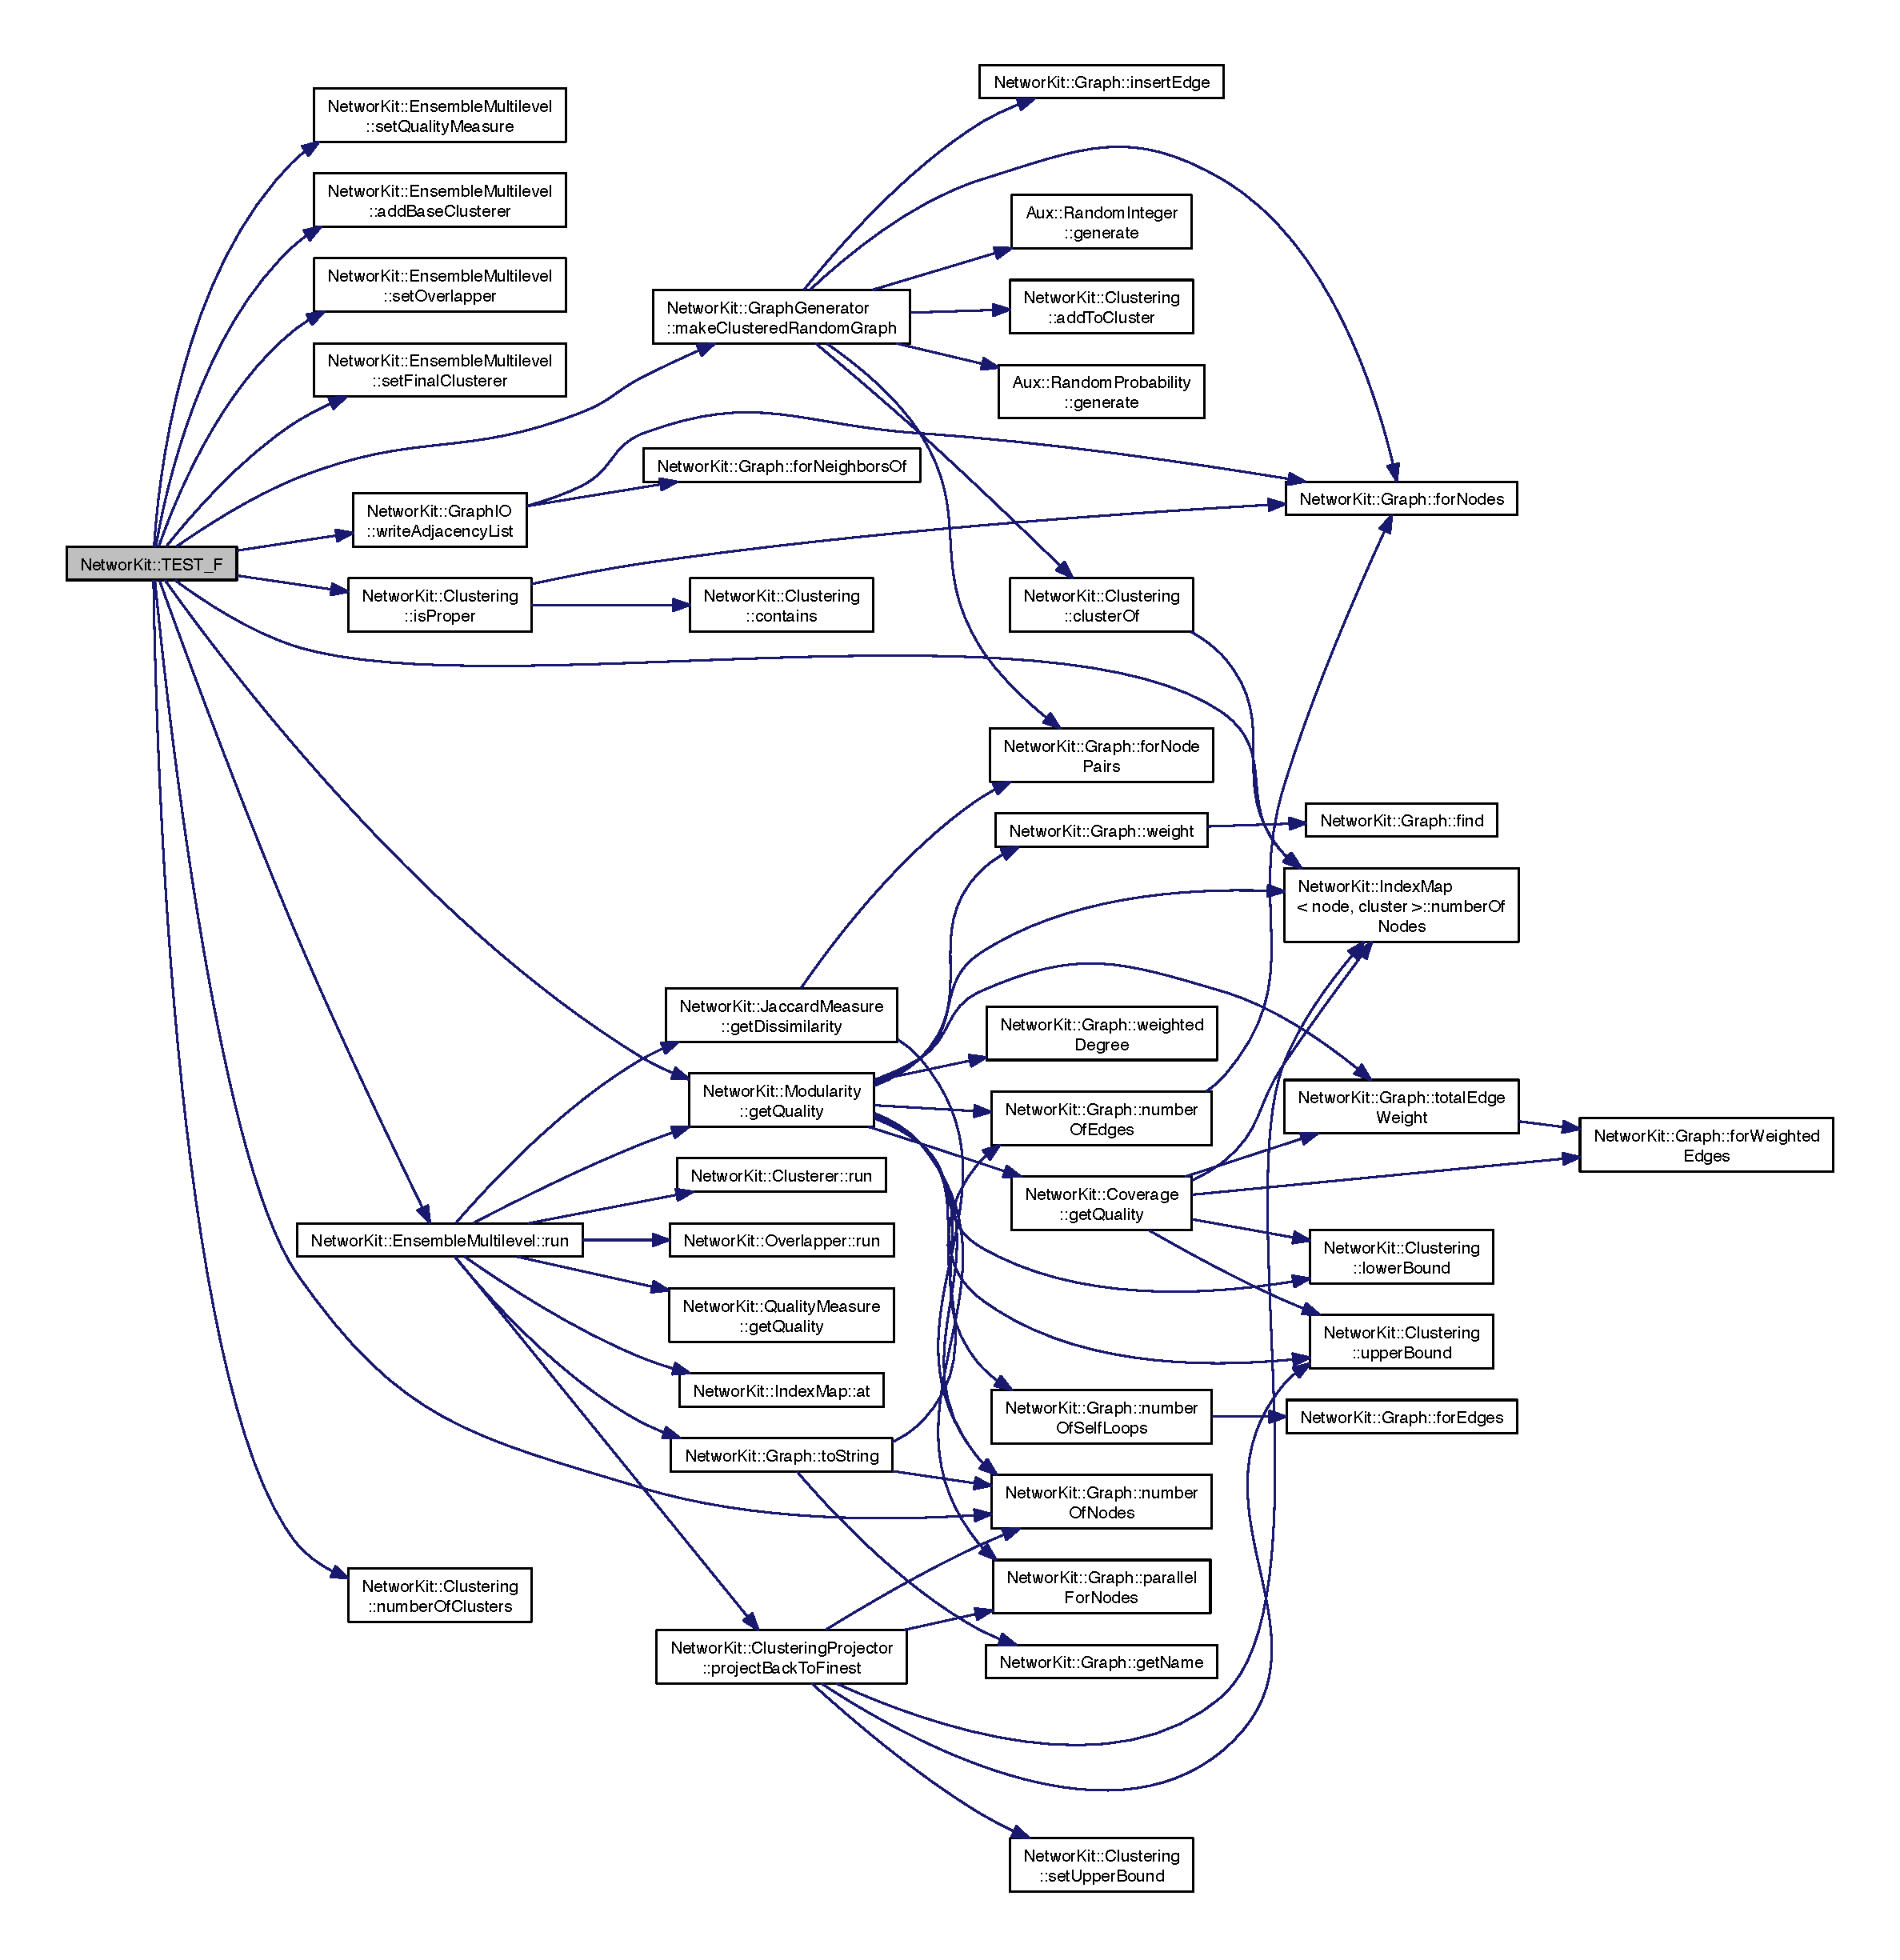
\includegraphics[width=350pt]{namespace_networ_kit_a564f49207cf5c5bc26f822ab61e487a1_cgraph}
\end{center}
\end{figure}


\hypertarget{namespace_networ_kit_adc6014d7776384a91125e1adfc6821d1}{\index{Networ\-Kit@{Networ\-Kit}!T\-E\-S\-T\-\_\-\-F@{T\-E\-S\-T\-\_\-\-F}}
\index{T\-E\-S\-T\-\_\-\-F@{T\-E\-S\-T\-\_\-\-F}!NetworKit@{Networ\-Kit}}
\subsubsection[{T\-E\-S\-T\-\_\-\-F}]{\setlength{\rightskip}{0pt plus 5cm}Networ\-Kit\-::\-T\-E\-S\-T\-\_\-\-F (
\begin{DoxyParamCaption}
\item[{Input\-G\-Test}]{, }
\item[{test\-Graph\-I\-O\-Edge\-List}]{}
\end{DoxyParamCaption}
)}}\label{namespace_networ_kit_adc6014d7776384a91125e1adfc6821d1}


Definition at line 12 of file Input\-G\-Test.\-cpp.



Here is the call graph for this function\-:\nopagebreak
\begin{figure}[H]
\begin{center}
\leavevmode
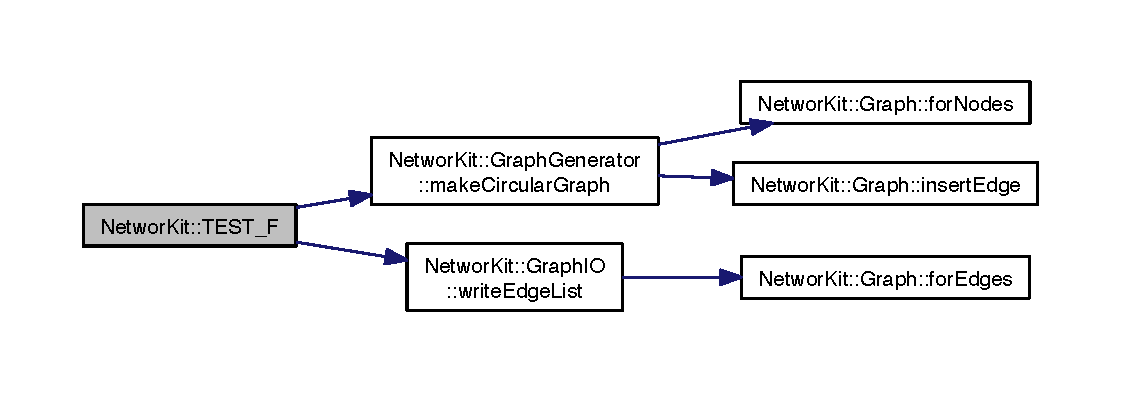
\includegraphics[width=350pt]{namespace_networ_kit_adc6014d7776384a91125e1adfc6821d1_cgraph}
\end{center}
\end{figure}


\hypertarget{namespace_networ_kit_af9839fafa3ea33c533ac5c910de4d716}{\index{Networ\-Kit@{Networ\-Kit}!T\-E\-S\-T\-\_\-\-F@{T\-E\-S\-T\-\_\-\-F}}
\index{T\-E\-S\-T\-\_\-\-F@{T\-E\-S\-T\-\_\-\-F}!NetworKit@{Networ\-Kit}}
\subsubsection[{T\-E\-S\-T\-\_\-\-F}]{\setlength{\rightskip}{0pt plus 5cm}Networ\-Kit\-::\-T\-E\-S\-T\-\_\-\-F (
\begin{DoxyParamCaption}
\item[{Coarsening\-G\-Test}]{, }
\item[{test\-Cluster\-Contracter}]{}
\end{DoxyParamCaption}
)}}\label{namespace_networ_kit_af9839fafa3ea33c533ac5c910de4d716}


Definition at line 12 of file Coarsening\-G\-Test.\-cpp.



Here is the call graph for this function\-:\nopagebreak
\begin{figure}[H]
\begin{center}
\leavevmode
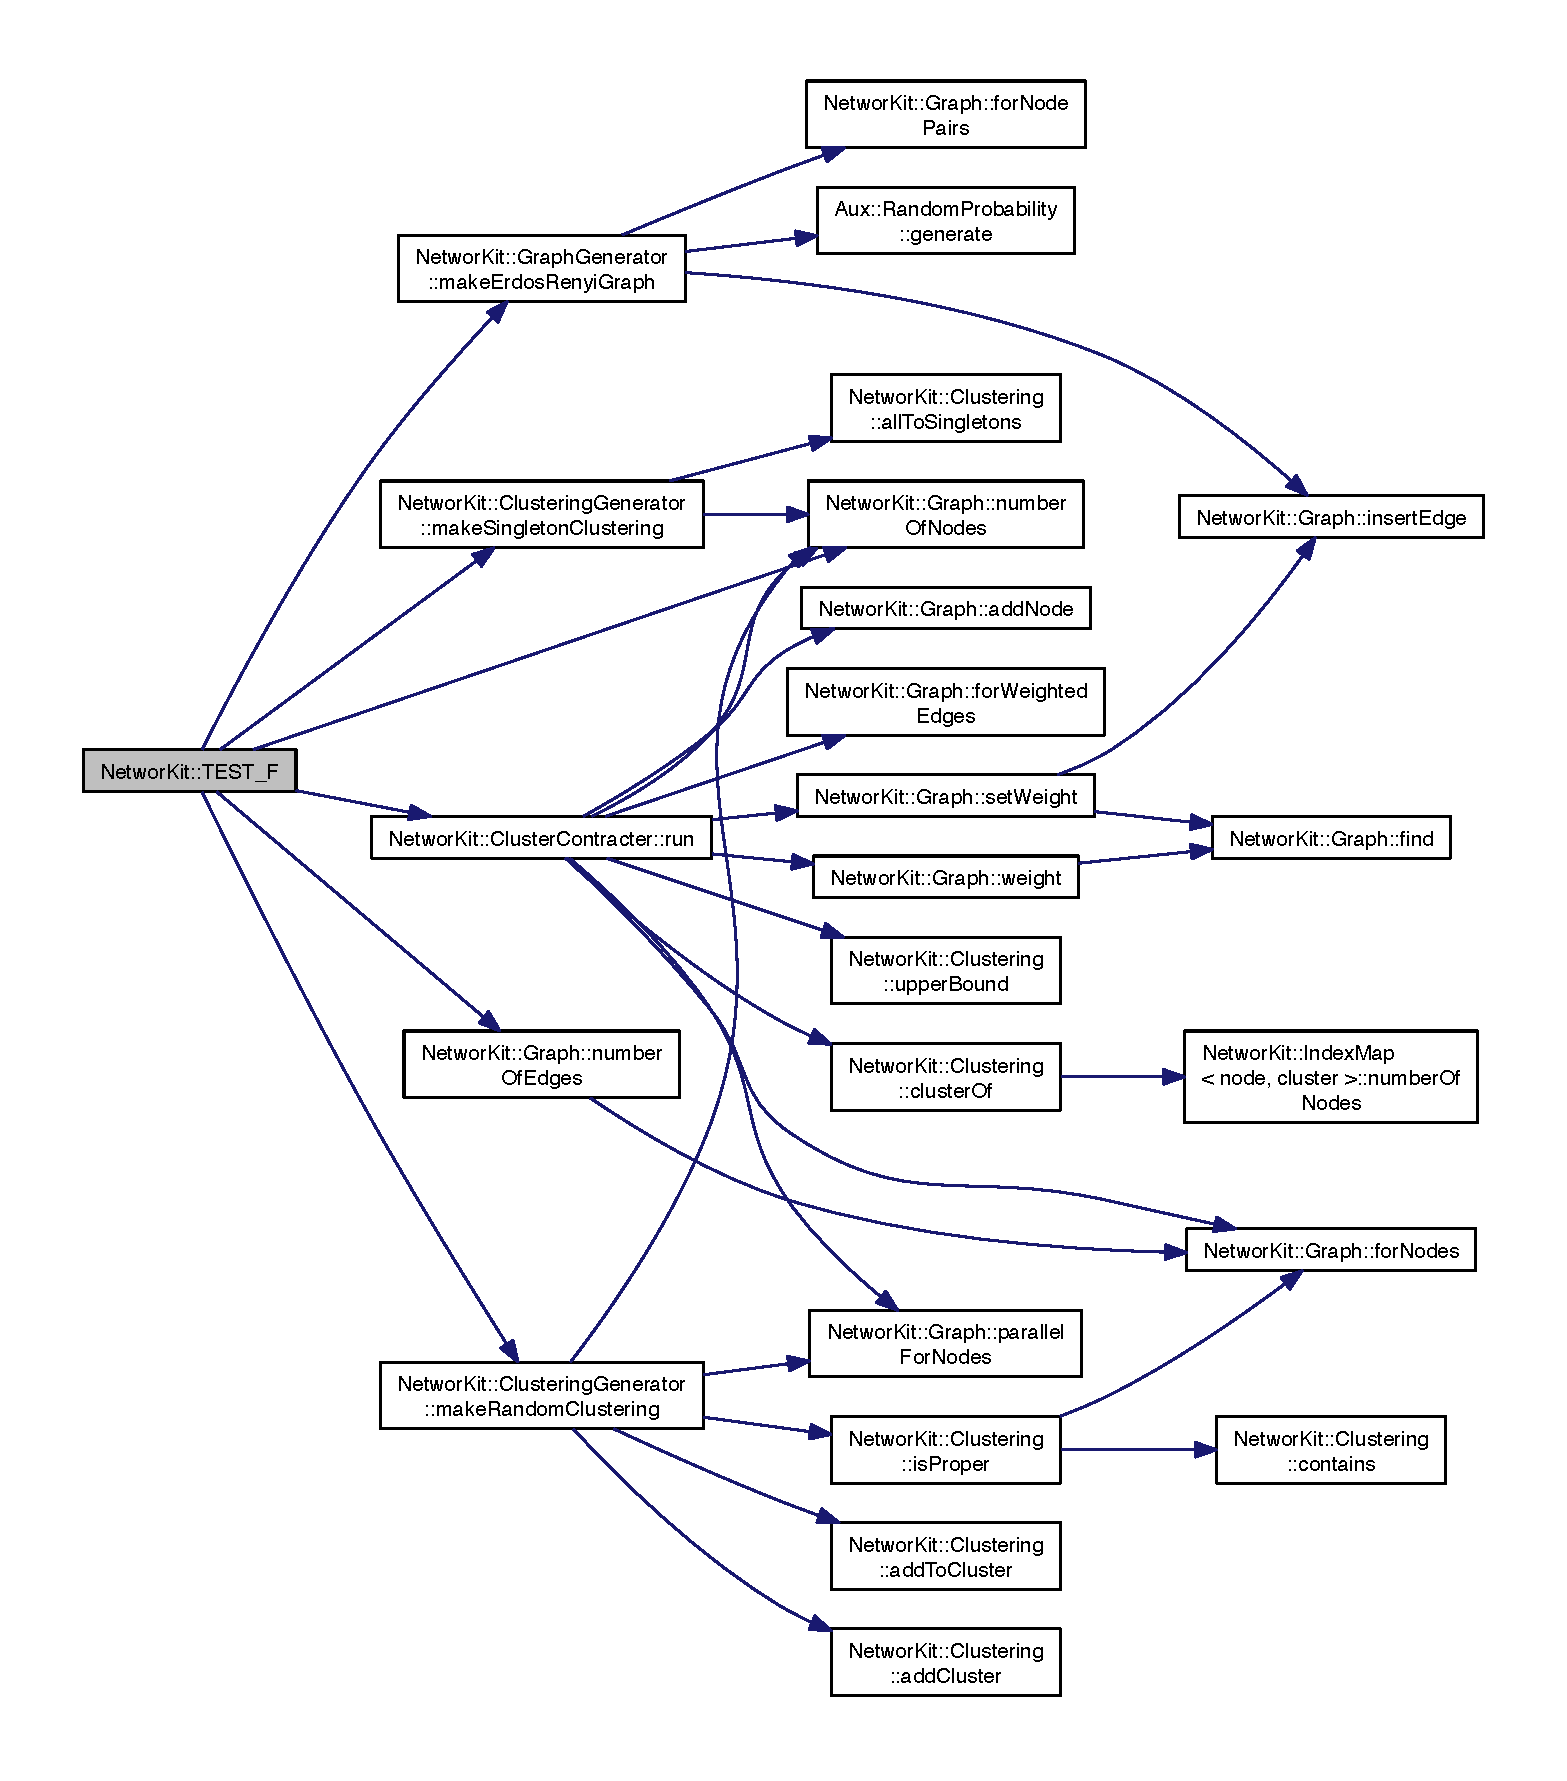
\includegraphics[width=350pt]{namespace_networ_kit_af9839fafa3ea33c533ac5c910de4d716_cgraph}
\end{center}
\end{figure}


\hypertarget{namespace_networ_kit_ac88ca919fafae77b31d9701fe3fbf41f}{\index{Networ\-Kit@{Networ\-Kit}!T\-E\-S\-T\-\_\-\-F@{T\-E\-S\-T\-\_\-\-F}}
\index{T\-E\-S\-T\-\_\-\-F@{T\-E\-S\-T\-\_\-\-F}!NetworKit@{Networ\-Kit}}
\subsubsection[{T\-E\-S\-T\-\_\-\-F}]{\setlength{\rightskip}{0pt plus 5cm}Networ\-Kit\-::\-T\-E\-S\-T\-\_\-\-F (
\begin{DoxyParamCaption}
\item[{Clustering\-Algo\-G\-Test}]{, }
\item[{test\-Label\-Propagation\-On\-Uniform\-Graph}]{}
\end{DoxyParamCaption}
)}}\label{namespace_networ_kit_ac88ca919fafae77b31d9701fe3fbf41f}


Definition at line 12 of file Clustering\-Algo\-G\-Test.\-cpp.



Here is the call graph for this function\-:\nopagebreak
\begin{figure}[H]
\begin{center}
\leavevmode
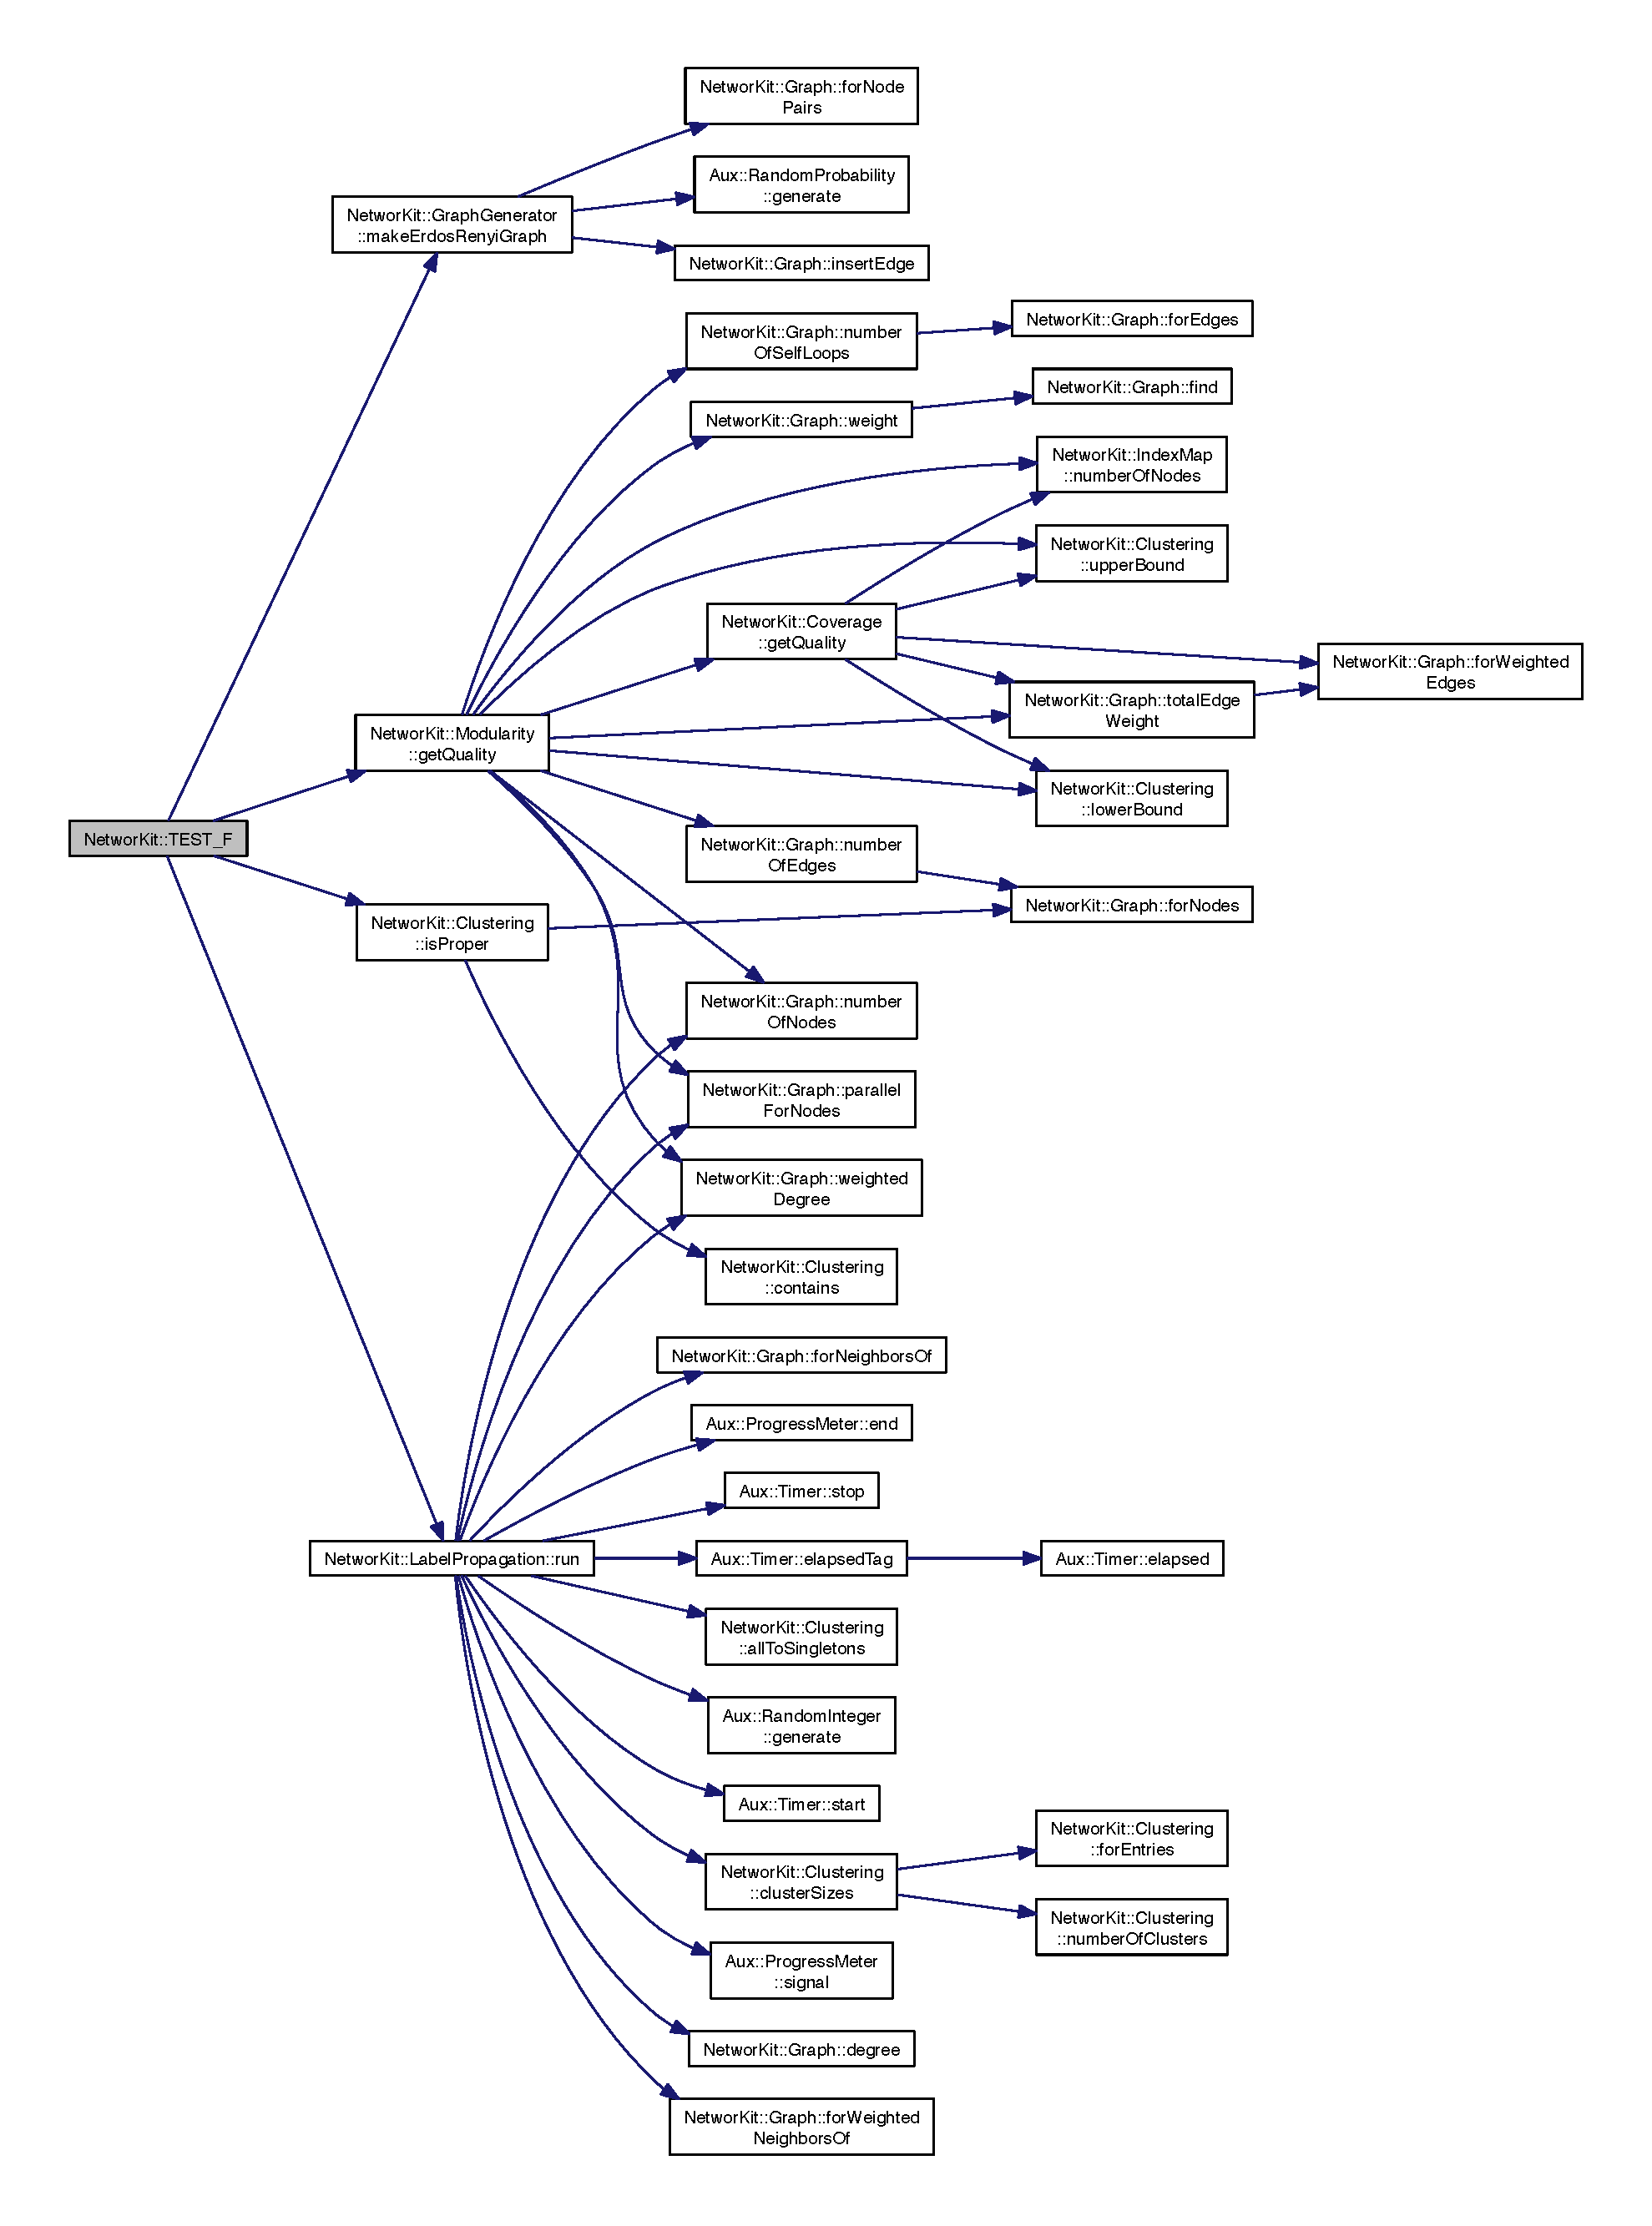
\includegraphics[width=350pt]{namespace_networ_kit_ac88ca919fafae77b31d9701fe3fbf41f_cgraph}
\end{center}
\end{figure}


\hypertarget{namespace_networ_kit_ae7dc36fc4dfa31d3d84b0bb505655ad8}{\index{Networ\-Kit@{Networ\-Kit}!T\-E\-S\-T\-\_\-\-F@{T\-E\-S\-T\-\_\-\-F}}
\index{T\-E\-S\-T\-\_\-\-F@{T\-E\-S\-T\-\_\-\-F}!NetworKit@{Networ\-Kit}}
\subsubsection[{T\-E\-S\-T\-\_\-\-F}]{\setlength{\rightskip}{0pt plus 5cm}Networ\-Kit\-::\-T\-E\-S\-T\-\_\-\-F (
\begin{DoxyParamCaption}
\item[{Overlap\-G\-Test}]{, }
\item[{test\-Region\-Growing\-Overlapper\-On\-One\-Clustering}]{}
\end{DoxyParamCaption}
)}}\label{namespace_networ_kit_ae7dc36fc4dfa31d3d84b0bb505655ad8}


Definition at line 13 of file Overlap\-G\-Test.\-cpp.



Here is the call graph for this function\-:\nopagebreak
\begin{figure}[H]
\begin{center}
\leavevmode
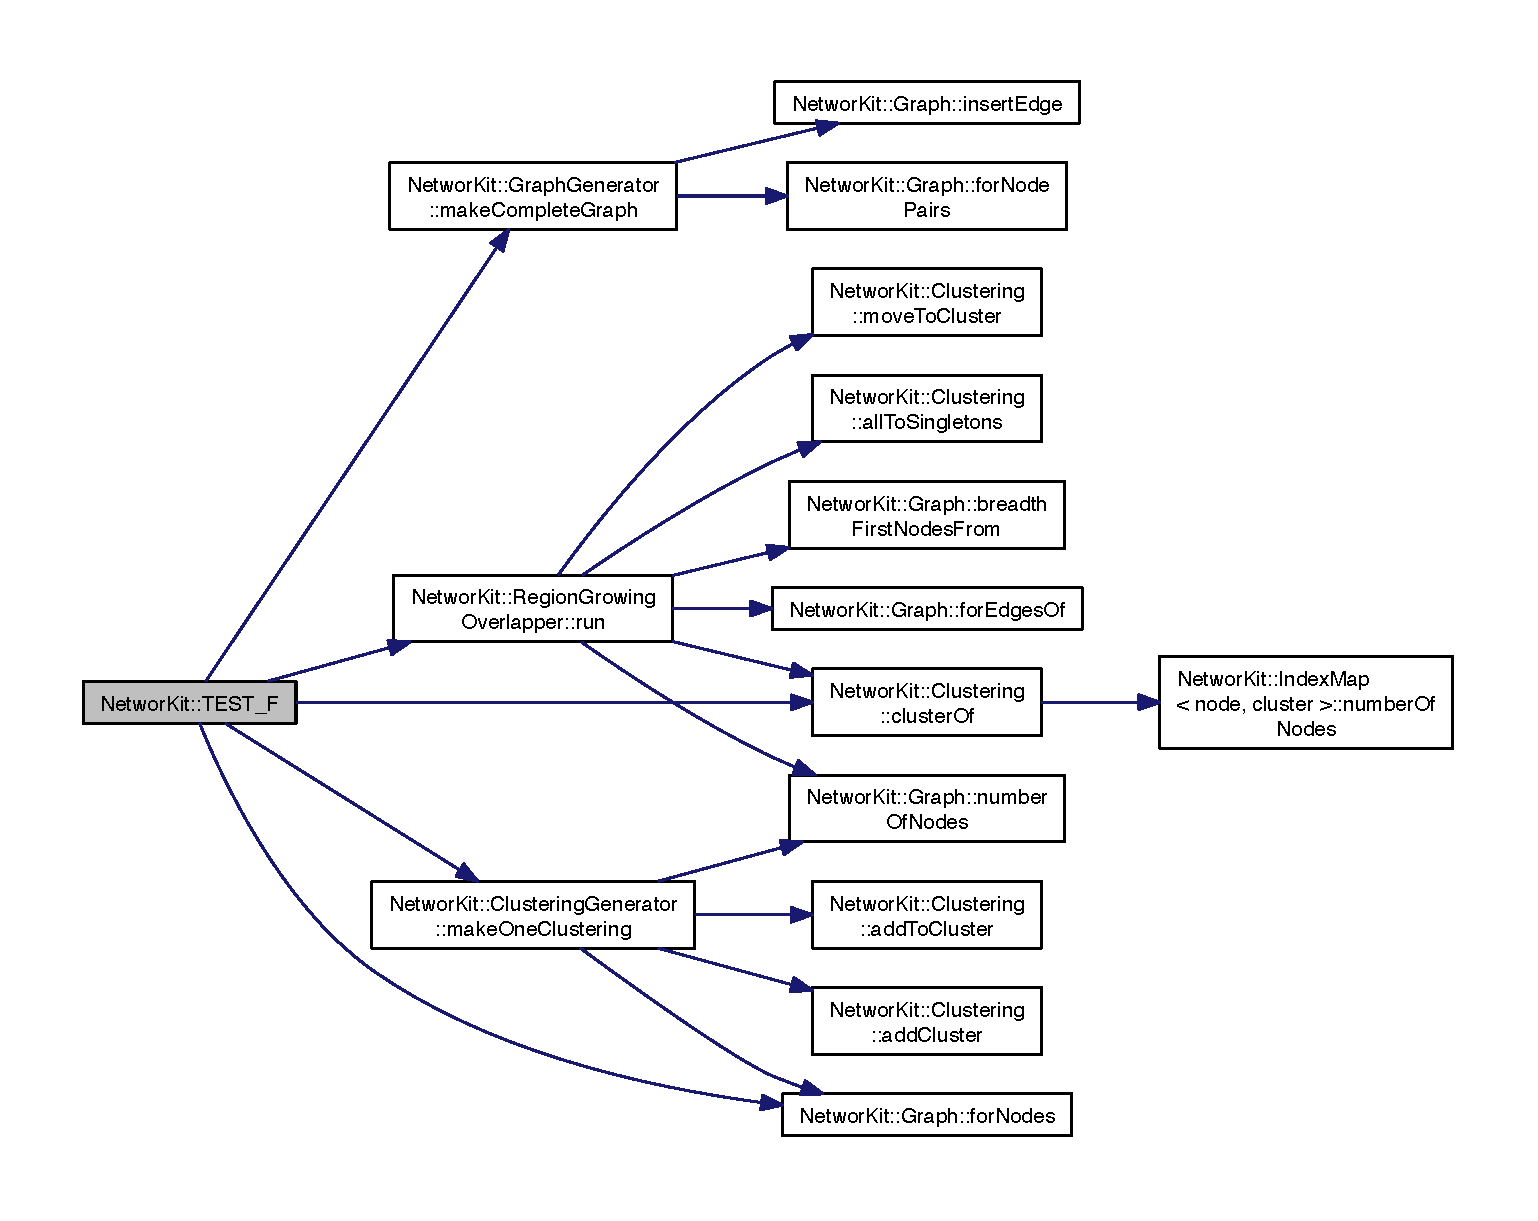
\includegraphics[width=350pt]{namespace_networ_kit_ae7dc36fc4dfa31d3d84b0bb505655ad8_cgraph}
\end{center}
\end{figure}


\hypertarget{namespace_networ_kit_ae7329d30d6284a0d4aee6045ad5fa91a}{\index{Networ\-Kit@{Networ\-Kit}!T\-E\-S\-T\-\_\-\-F@{T\-E\-S\-T\-\_\-\-F}}
\index{T\-E\-S\-T\-\_\-\-F@{T\-E\-S\-T\-\_\-\-F}!NetworKit@{Networ\-Kit}}
\subsubsection[{T\-E\-S\-T\-\_\-\-F}]{\setlength{\rightskip}{0pt plus 5cm}Networ\-Kit\-::\-T\-E\-S\-T\-\_\-\-F (
\begin{DoxyParamCaption}
\item[{Clustering\-G\-Test}]{, }
\item[{test\-Modularity}]{}
\end{DoxyParamCaption}
)}}\label{namespace_networ_kit_ae7329d30d6284a0d4aee6045ad5fa91a}


Definition at line 14 of file Clustering\-G\-Test.\-cpp.



Here is the call graph for this function\-:\nopagebreak
\begin{figure}[H]
\begin{center}
\leavevmode
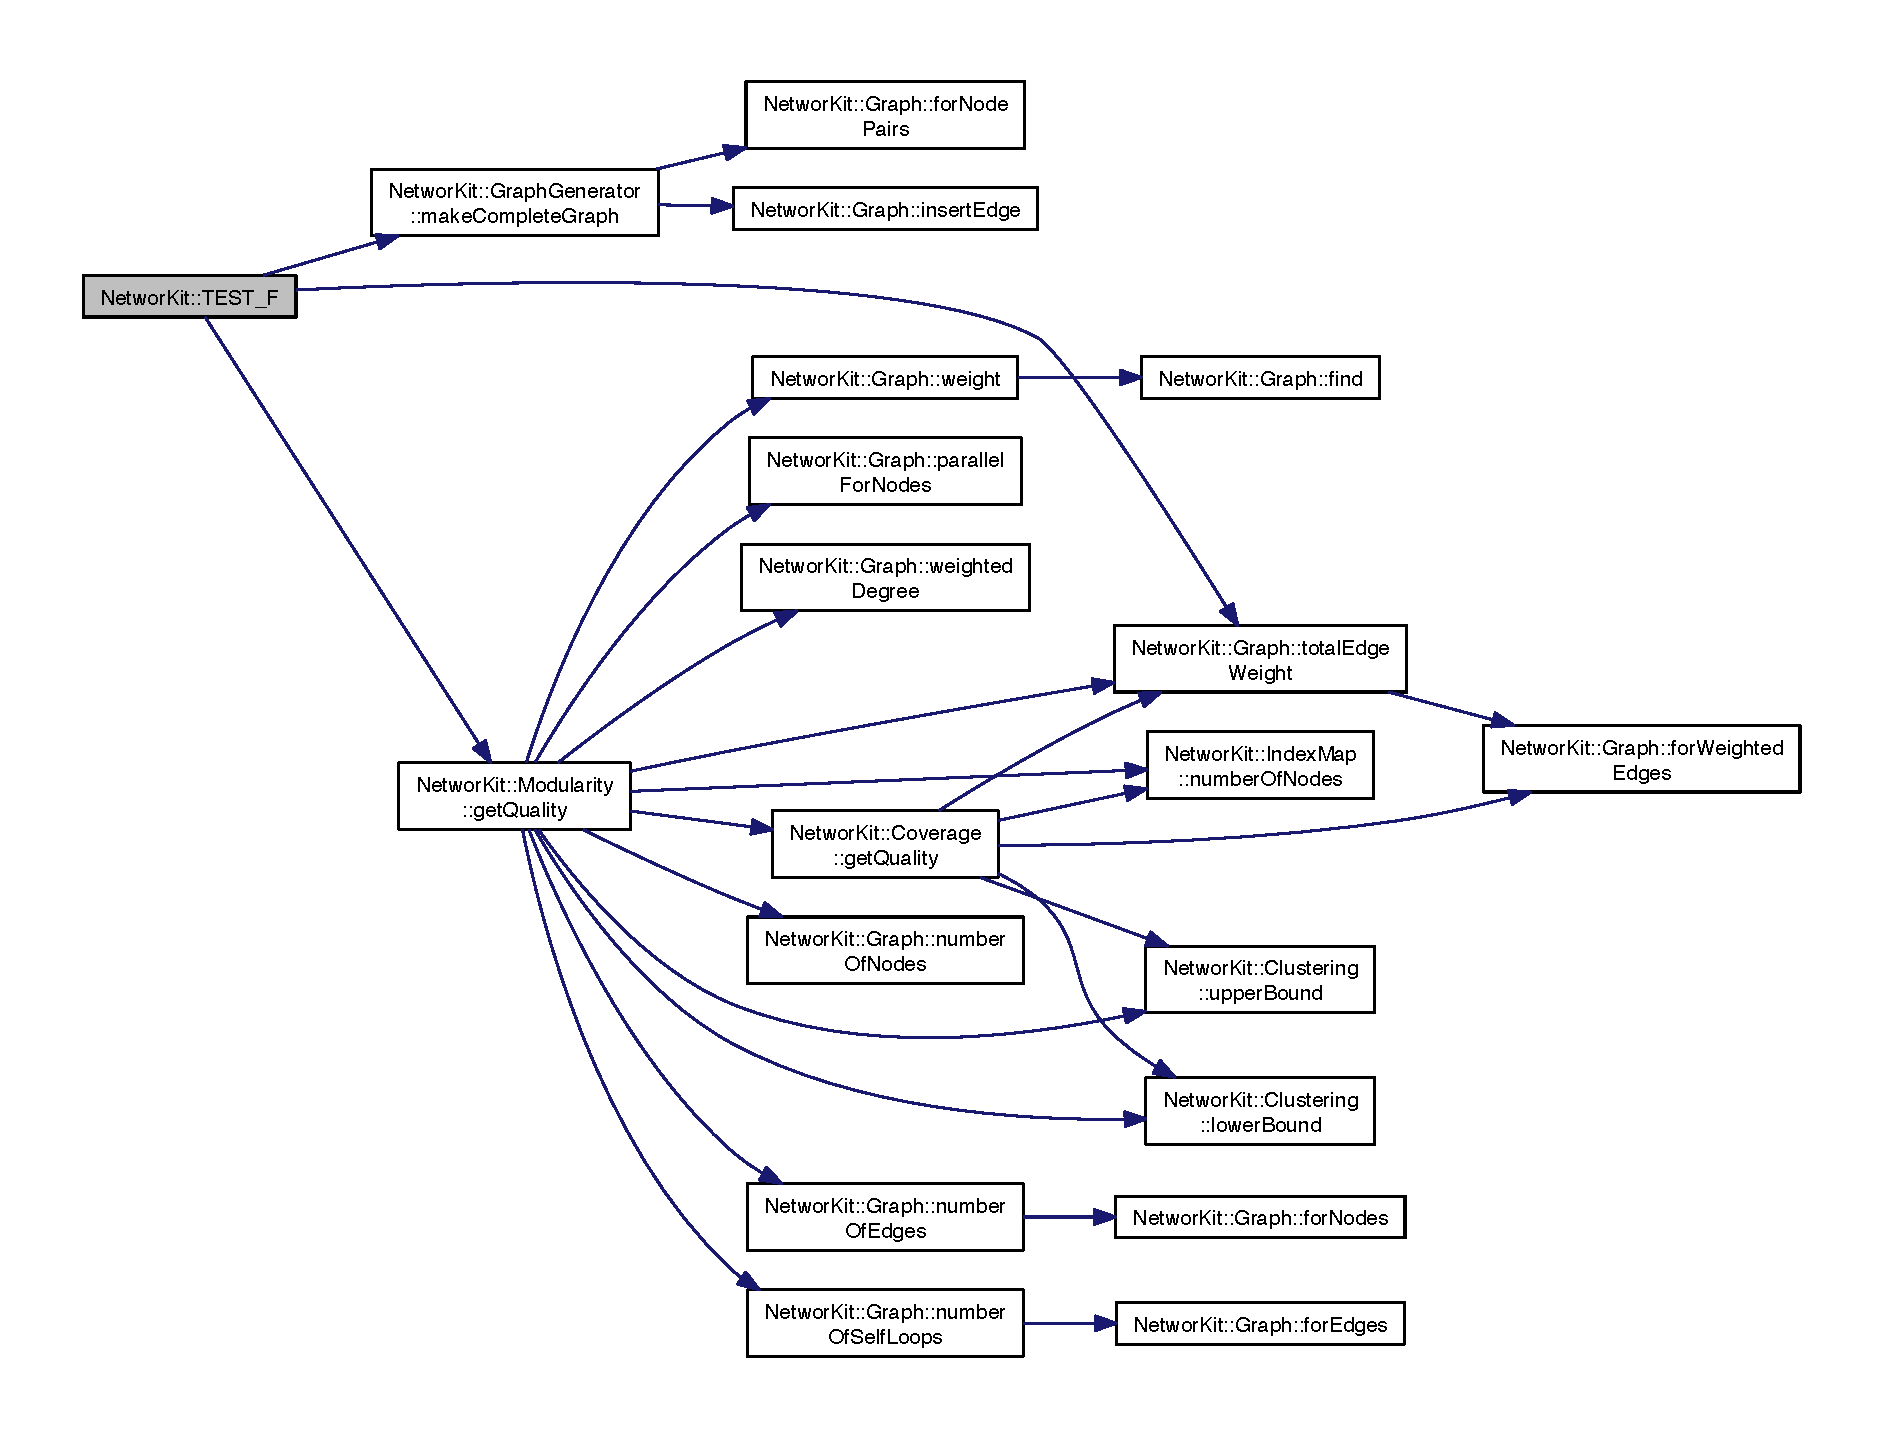
\includegraphics[width=350pt]{namespace_networ_kit_ae7329d30d6284a0d4aee6045ad5fa91a_cgraph}
\end{center}
\end{figure}


\hypertarget{namespace_networ_kit_a2e6dc85b94615593bec85ab0d961f7a5}{\index{Networ\-Kit@{Networ\-Kit}!T\-E\-S\-T\-\_\-\-F@{T\-E\-S\-T\-\_\-\-F}}
\index{T\-E\-S\-T\-\_\-\-F@{T\-E\-S\-T\-\_\-\-F}!NetworKit@{Networ\-Kit}}
\subsubsection[{T\-E\-S\-T\-\_\-\-F}]{\setlength{\rightskip}{0pt plus 5cm}Networ\-Kit\-::\-T\-E\-S\-T\-\_\-\-F (
\begin{DoxyParamCaption}
\item[{Graph\-Generator\-G\-Test}]{, }
\item[{test\-Barabasi\-Albert}]{}
\end{DoxyParamCaption}
)}}\label{namespace_networ_kit_a2e6dc85b94615593bec85ab0d961f7a5}


Definition at line 21 of file Graph\-Generator\-G\-Test.\-cpp.

\hypertarget{namespace_networ_kit_a1380d5e4eef1fb7e4e4eb7456506b457}{\index{Networ\-Kit@{Networ\-Kit}!T\-E\-S\-T\-\_\-\-F@{T\-E\-S\-T\-\_\-\-F}}
\index{T\-E\-S\-T\-\_\-\-F@{T\-E\-S\-T\-\_\-\-F}!NetworKit@{Networ\-Kit}}
\subsubsection[{T\-E\-S\-T\-\_\-\-F}]{\setlength{\rightskip}{0pt plus 5cm}Networ\-Kit\-::\-T\-E\-S\-T\-\_\-\-F (
\begin{DoxyParamCaption}
\item[{Graph2\-Benchmark}]{, }
\item[{graph\-Construction}]{}
\end{DoxyParamCaption}
)}}\label{namespace_networ_kit_a1380d5e4eef1fb7e4e4eb7456506b457}


Definition at line 21 of file Graph2\-Benchmark.\-cpp.



Here is the call graph for this function\-:\nopagebreak
\begin{figure}[H]
\begin{center}
\leavevmode
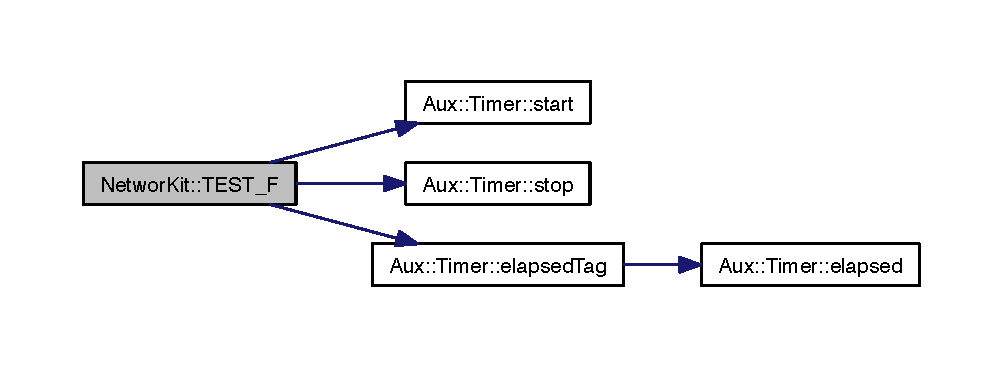
\includegraphics[width=350pt]{namespace_networ_kit_a1380d5e4eef1fb7e4e4eb7456506b457_cgraph}
\end{center}
\end{figure}


\hypertarget{namespace_networ_kit_a68b5958ff9c52ac3f38f0cd54125ae99}{\index{Networ\-Kit@{Networ\-Kit}!T\-E\-S\-T\-\_\-\-F@{T\-E\-S\-T\-\_\-\-F}}
\index{T\-E\-S\-T\-\_\-\-F@{T\-E\-S\-T\-\_\-\-F}!NetworKit@{Networ\-Kit}}
\subsubsection[{T\-E\-S\-T\-\_\-\-F}]{\setlength{\rightskip}{0pt plus 5cm}Networ\-Kit\-::\-T\-E\-S\-T\-\_\-\-F (
\begin{DoxyParamCaption}
\item[{Graph2\-G\-Test}]{, }
\item[{test\-Number\-Of\-Nodes}]{}
\end{DoxyParamCaption}
)}}\label{namespace_networ_kit_a68b5958ff9c52ac3f38f0cd54125ae99}


Definition at line 22 of file Graph2\-G\-Test.\-cpp.



Here is the call graph for this function\-:\nopagebreak
\begin{figure}[H]
\begin{center}
\leavevmode
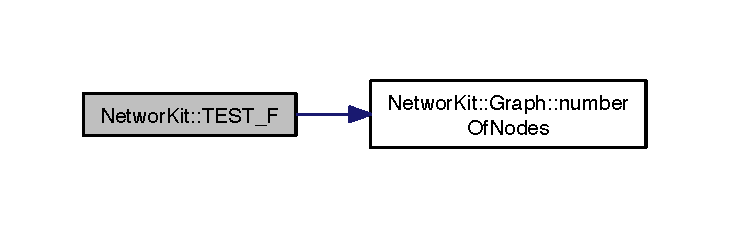
\includegraphics[width=350pt]{namespace_networ_kit_a68b5958ff9c52ac3f38f0cd54125ae99_cgraph}
\end{center}
\end{figure}


\hypertarget{namespace_networ_kit_a4fc0bfd7f1d51fb53b57d971efdd5b7a}{\index{Networ\-Kit@{Networ\-Kit}!T\-E\-S\-T\-\_\-\-F@{T\-E\-S\-T\-\_\-\-F}}
\index{T\-E\-S\-T\-\_\-\-F@{T\-E\-S\-T\-\_\-\-F}!NetworKit@{Networ\-Kit}}
\subsubsection[{T\-E\-S\-T\-\_\-\-F}]{\setlength{\rightskip}{0pt plus 5cm}Networ\-Kit\-::\-T\-E\-S\-T\-\_\-\-F (
\begin{DoxyParamCaption}
\item[{Independent\-Set\-G\-Test}]{, }
\item[{test\-Luby}]{}
\end{DoxyParamCaption}
)}}\label{namespace_networ_kit_a4fc0bfd7f1d51fb53b57d971efdd5b7a}


Definition at line 22 of file Independent\-Set\-G\-Test.\-cpp.



Here is the call graph for this function\-:\nopagebreak
\begin{figure}[H]
\begin{center}
\leavevmode
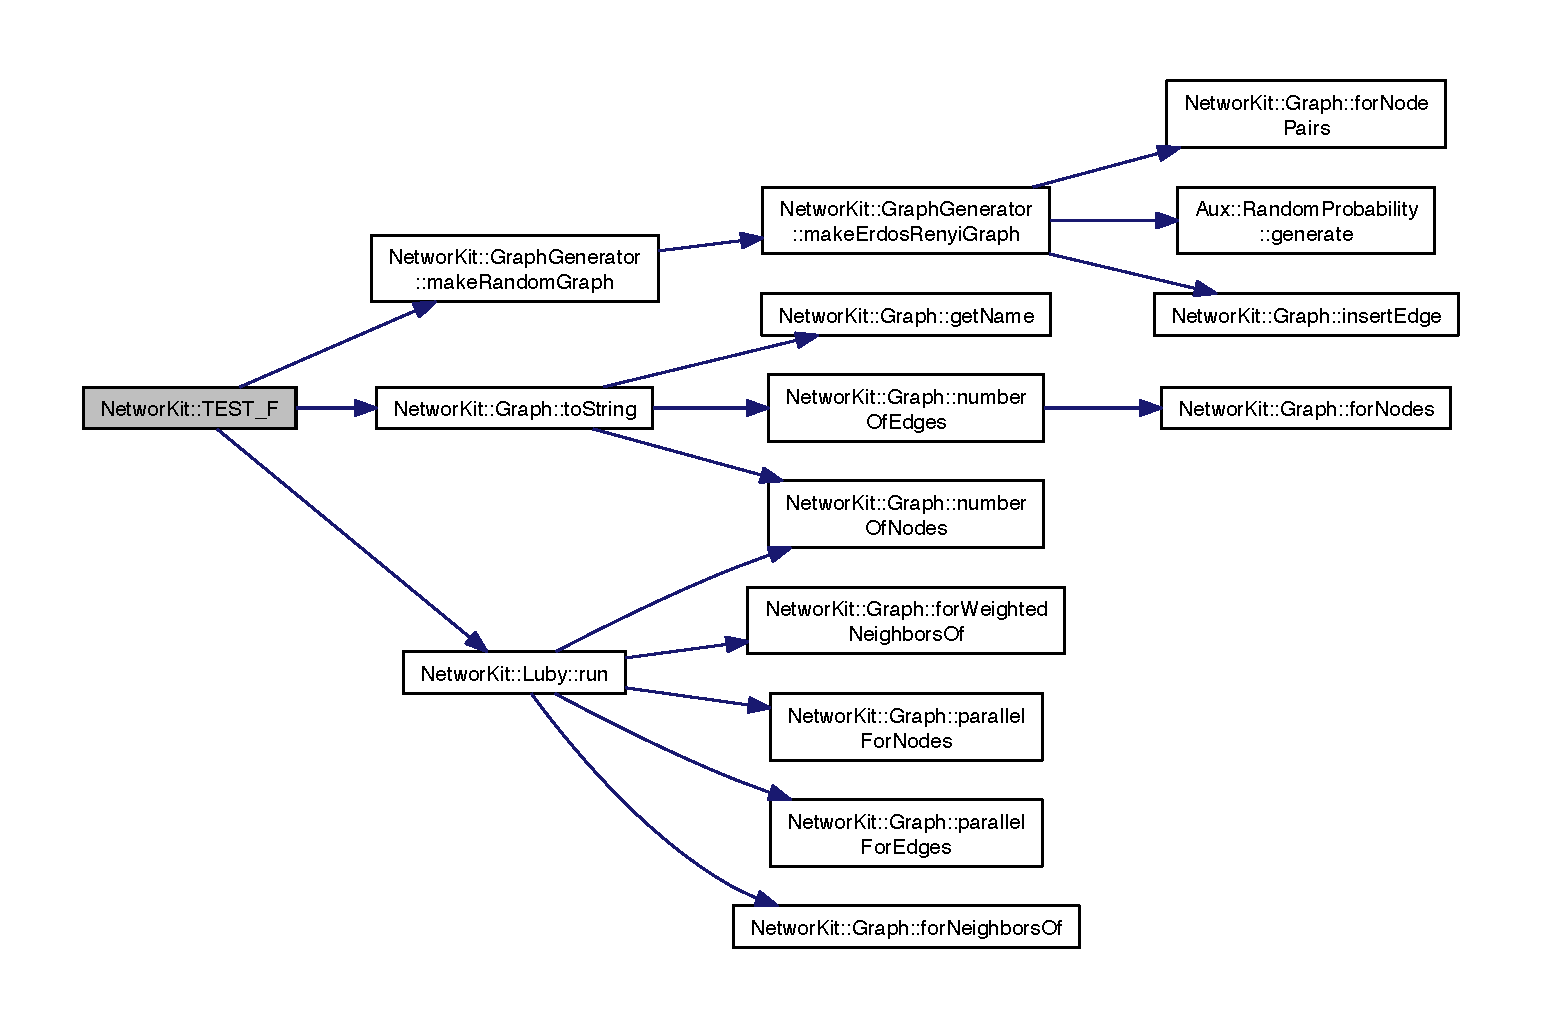
\includegraphics[width=350pt]{namespace_networ_kit_a4fc0bfd7f1d51fb53b57d971efdd5b7a_cgraph}
\end{center}
\end{figure}


\hypertarget{namespace_networ_kit_aee97d3f13ee3f1c38d22f87787977f02}{\index{Networ\-Kit@{Networ\-Kit}!T\-E\-S\-T\-\_\-\-F@{T\-E\-S\-T\-\_\-\-F}}
\index{T\-E\-S\-T\-\_\-\-F@{T\-E\-S\-T\-\_\-\-F}!NetworKit@{Networ\-Kit}}
\subsubsection[{T\-E\-S\-T\-\_\-\-F}]{\setlength{\rightskip}{0pt plus 5cm}Networ\-Kit\-::\-T\-E\-S\-T\-\_\-\-F (
\begin{DoxyParamCaption}
\item[{I\-O\-Benchmark}]{, }
\item[{time\-M\-E\-T\-I\-S\-Graph\-Reader}]{}
\end{DoxyParamCaption}
)}}\label{namespace_networ_kit_aee97d3f13ee3f1c38d22f87787977f02}


Definition at line 22 of file I\-O\-Benchmark.\-cpp.



Here is the call graph for this function\-:\nopagebreak
\begin{figure}[H]
\begin{center}
\leavevmode
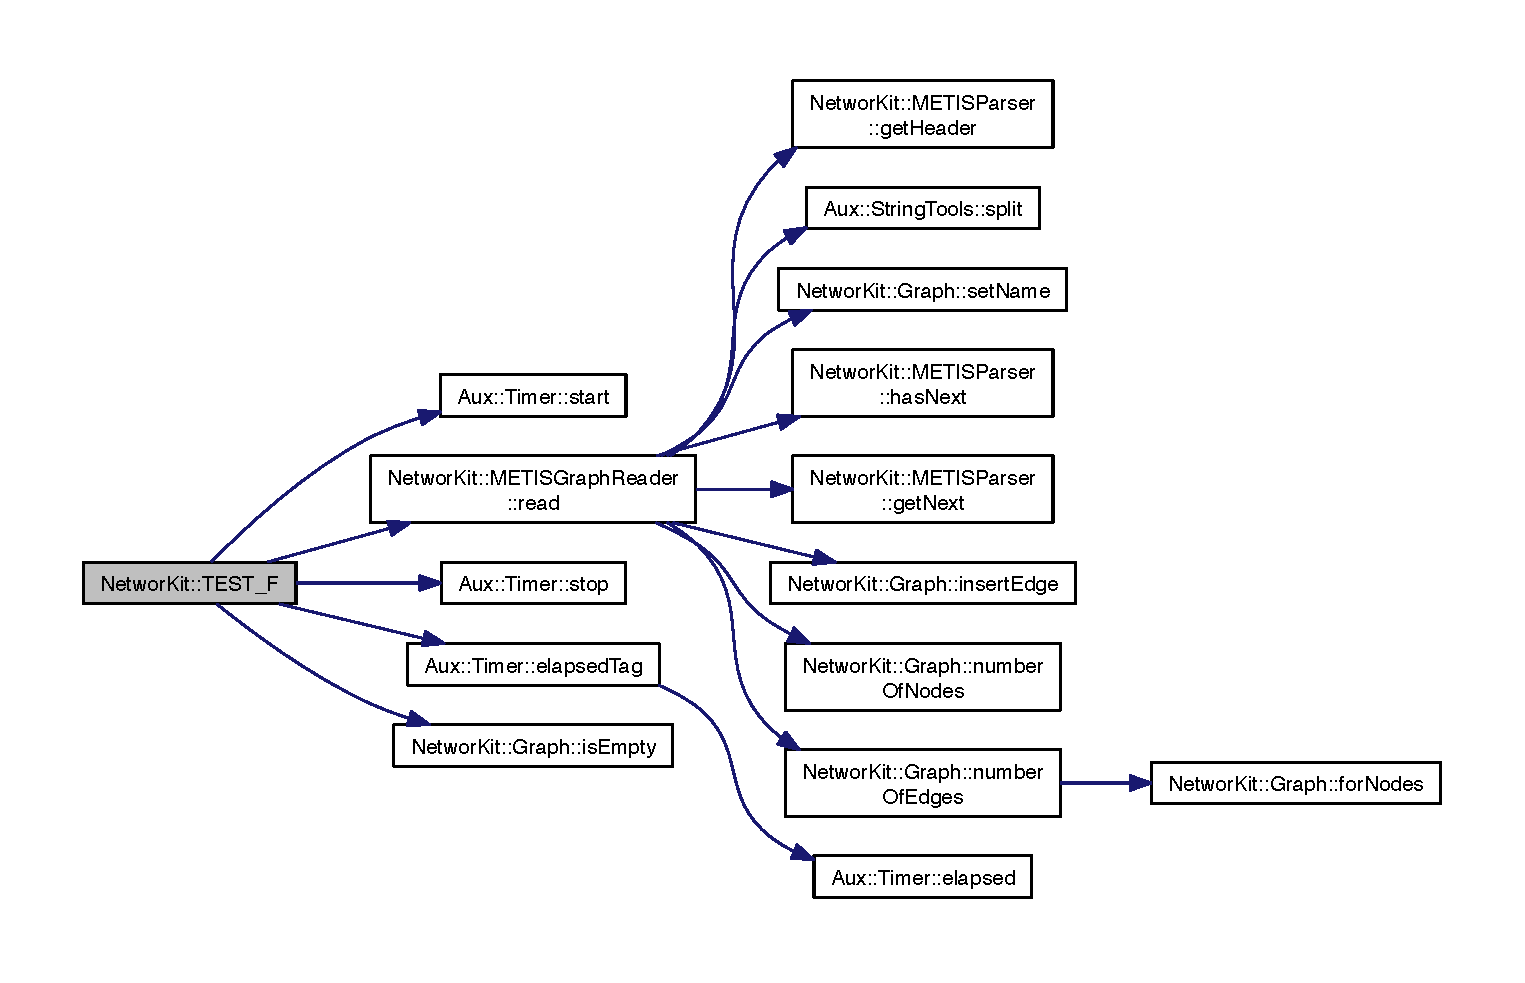
\includegraphics[width=350pt]{namespace_networ_kit_aee97d3f13ee3f1c38d22f87787977f02_cgraph}
\end{center}
\end{figure}


\hypertarget{namespace_networ_kit_af04baad3988791b80bd77d2a8e1f3fde}{\index{Networ\-Kit@{Networ\-Kit}!T\-E\-S\-T\-\_\-\-F@{T\-E\-S\-T\-\_\-\-F}}
\index{T\-E\-S\-T\-\_\-\-F@{T\-E\-S\-T\-\_\-\-F}!NetworKit@{Networ\-Kit}}
\subsubsection[{T\-E\-S\-T\-\_\-\-F}]{\setlength{\rightskip}{0pt plus 5cm}Networ\-Kit\-::\-T\-E\-S\-T\-\_\-\-F (
\begin{DoxyParamCaption}
\item[{Basics\-Benchmark}]{, }
\item[{sequential\-Sum}]{}
\end{DoxyParamCaption}
)}}\label{namespace_networ_kit_af04baad3988791b80bd77d2a8e1f3fde}


Definition at line 23 of file Basics\-Benchmark.\-cpp.



Here is the call graph for this function\-:\nopagebreak
\begin{figure}[H]
\begin{center}
\leavevmode
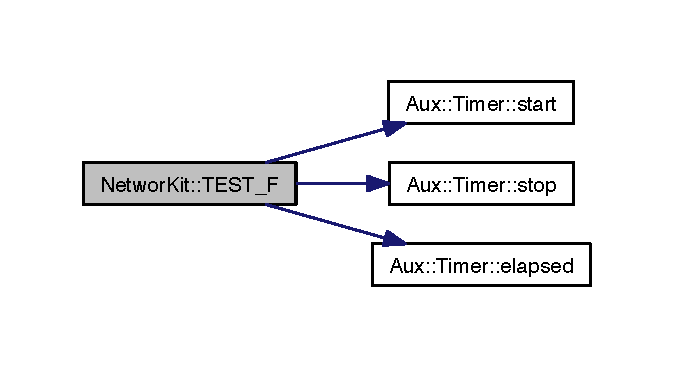
\includegraphics[width=324pt]{namespace_networ_kit_af04baad3988791b80bd77d2a8e1f3fde_cgraph}
\end{center}
\end{figure}


\hypertarget{namespace_networ_kit_ab3677f34b5d4ea16d7d6cf26b1917959}{\index{Networ\-Kit@{Networ\-Kit}!T\-E\-S\-T\-\_\-\-F@{T\-E\-S\-T\-\_\-\-F}}
\index{T\-E\-S\-T\-\_\-\-F@{T\-E\-S\-T\-\_\-\-F}!NetworKit@{Networ\-Kit}}
\subsubsection[{T\-E\-S\-T\-\_\-\-F}]{\setlength{\rightskip}{0pt plus 5cm}Networ\-Kit\-::\-T\-E\-S\-T\-\_\-\-F (
\begin{DoxyParamCaption}
\item[{Graph\-Benchmark}]{, }
\item[{edge\-Insertions\-\_\-noop\-\_\-seq}]{}
\end{DoxyParamCaption}
)}}\label{namespace_networ_kit_ab3677f34b5d4ea16d7d6cf26b1917959}


Definition at line 24 of file Graph\-Benchmark.\-cpp.



Here is the call graph for this function\-:\nopagebreak
\begin{figure}[H]
\begin{center}
\leavevmode
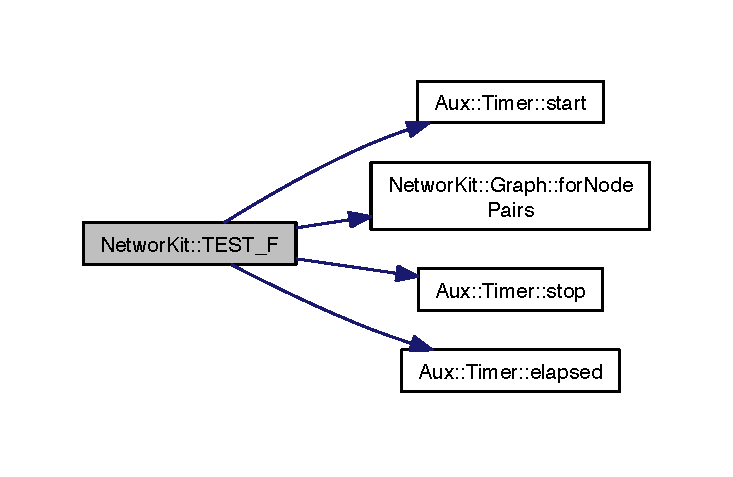
\includegraphics[width=350pt]{namespace_networ_kit_ab3677f34b5d4ea16d7d6cf26b1917959_cgraph}
\end{center}
\end{figure}


\hypertarget{namespace_networ_kit_a1badbd8faa22ba9d7da2c6acffb57897}{\index{Networ\-Kit@{Networ\-Kit}!T\-E\-S\-T\-\_\-\-F@{T\-E\-S\-T\-\_\-\-F}}
\index{T\-E\-S\-T\-\_\-\-F@{T\-E\-S\-T\-\_\-\-F}!NetworKit@{Networ\-Kit}}
\subsubsection[{T\-E\-S\-T\-\_\-\-F}]{\setlength{\rightskip}{0pt plus 5cm}Networ\-Kit\-::\-T\-E\-S\-T\-\_\-\-F (
\begin{DoxyParamCaption}
\item[{Input\-G\-Test}]{, }
\item[{test\-Graph\-I\-O\-Adjacency\-List}]{}
\end{DoxyParamCaption}
)}}\label{namespace_networ_kit_a1badbd8faa22ba9d7da2c6acffb57897}


Definition at line 27 of file Input\-G\-Test.\-cpp.



Here is the call graph for this function\-:\nopagebreak
\begin{figure}[H]
\begin{center}
\leavevmode
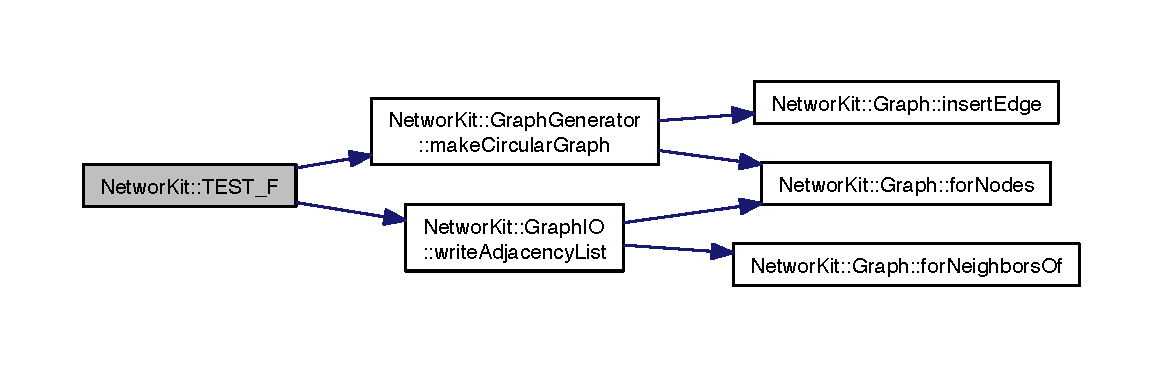
\includegraphics[width=350pt]{namespace_networ_kit_a1badbd8faa22ba9d7da2c6acffb57897_cgraph}
\end{center}
\end{figure}


\hypertarget{namespace_networ_kit_ad40252180bd36e0238b94f5576683951}{\index{Networ\-Kit@{Networ\-Kit}!T\-E\-S\-T\-\_\-\-F@{T\-E\-S\-T\-\_\-\-F}}
\index{T\-E\-S\-T\-\_\-\-F@{T\-E\-S\-T\-\_\-\-F}!NetworKit@{Networ\-Kit}}
\subsubsection[{T\-E\-S\-T\-\_\-\-F}]{\setlength{\rightskip}{0pt plus 5cm}Networ\-Kit\-::\-T\-E\-S\-T\-\_\-\-F (
\begin{DoxyParamCaption}
\item[{Graph\-G\-Test}]{, }
\item[{test\-Lambda\-Edge\-Iteration}]{}
\end{DoxyParamCaption}
)}}\label{namespace_networ_kit_ad40252180bd36e0238b94f5576683951}


Definition at line 30 of file Graph\-G\-Test.\-cpp.



Here is the call graph for this function\-:\nopagebreak
\begin{figure}[H]
\begin{center}
\leavevmode
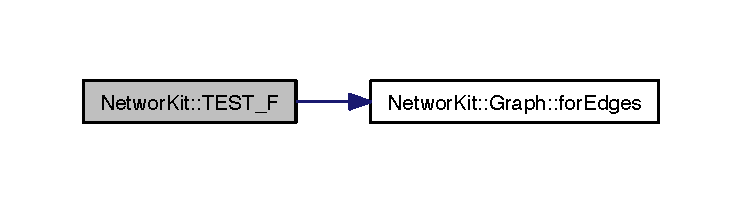
\includegraphics[width=350pt]{namespace_networ_kit_ad40252180bd36e0238b94f5576683951_cgraph}
\end{center}
\end{figure}


\hypertarget{namespace_networ_kit_a7590ba53b3c7daa9d805db41b17d979e}{\index{Networ\-Kit@{Networ\-Kit}!T\-E\-S\-T\-\_\-\-F@{T\-E\-S\-T\-\_\-\-F}}
\index{T\-E\-S\-T\-\_\-\-F@{T\-E\-S\-T\-\_\-\-F}!NetworKit@{Networ\-Kit}}
\subsubsection[{T\-E\-S\-T\-\_\-\-F}]{\setlength{\rightskip}{0pt plus 5cm}Networ\-Kit\-::\-T\-E\-S\-T\-\_\-\-F (
\begin{DoxyParamCaption}
\item[{Clustering\-Algo\-G\-Test}]{, }
\item[{test\-Label\-Propagation\-On\-Clustered\-Graph\-\_\-\-For\-Number\-Of\-Clusters}]{}
\end{DoxyParamCaption}
)}}\label{namespace_networ_kit_a7590ba53b3c7daa9d805db41b17d979e}


Definition at line 30 of file Clustering\-Algo\-G\-Test.\-cpp.



Here is the call graph for this function\-:\nopagebreak
\begin{figure}[H]
\begin{center}
\leavevmode
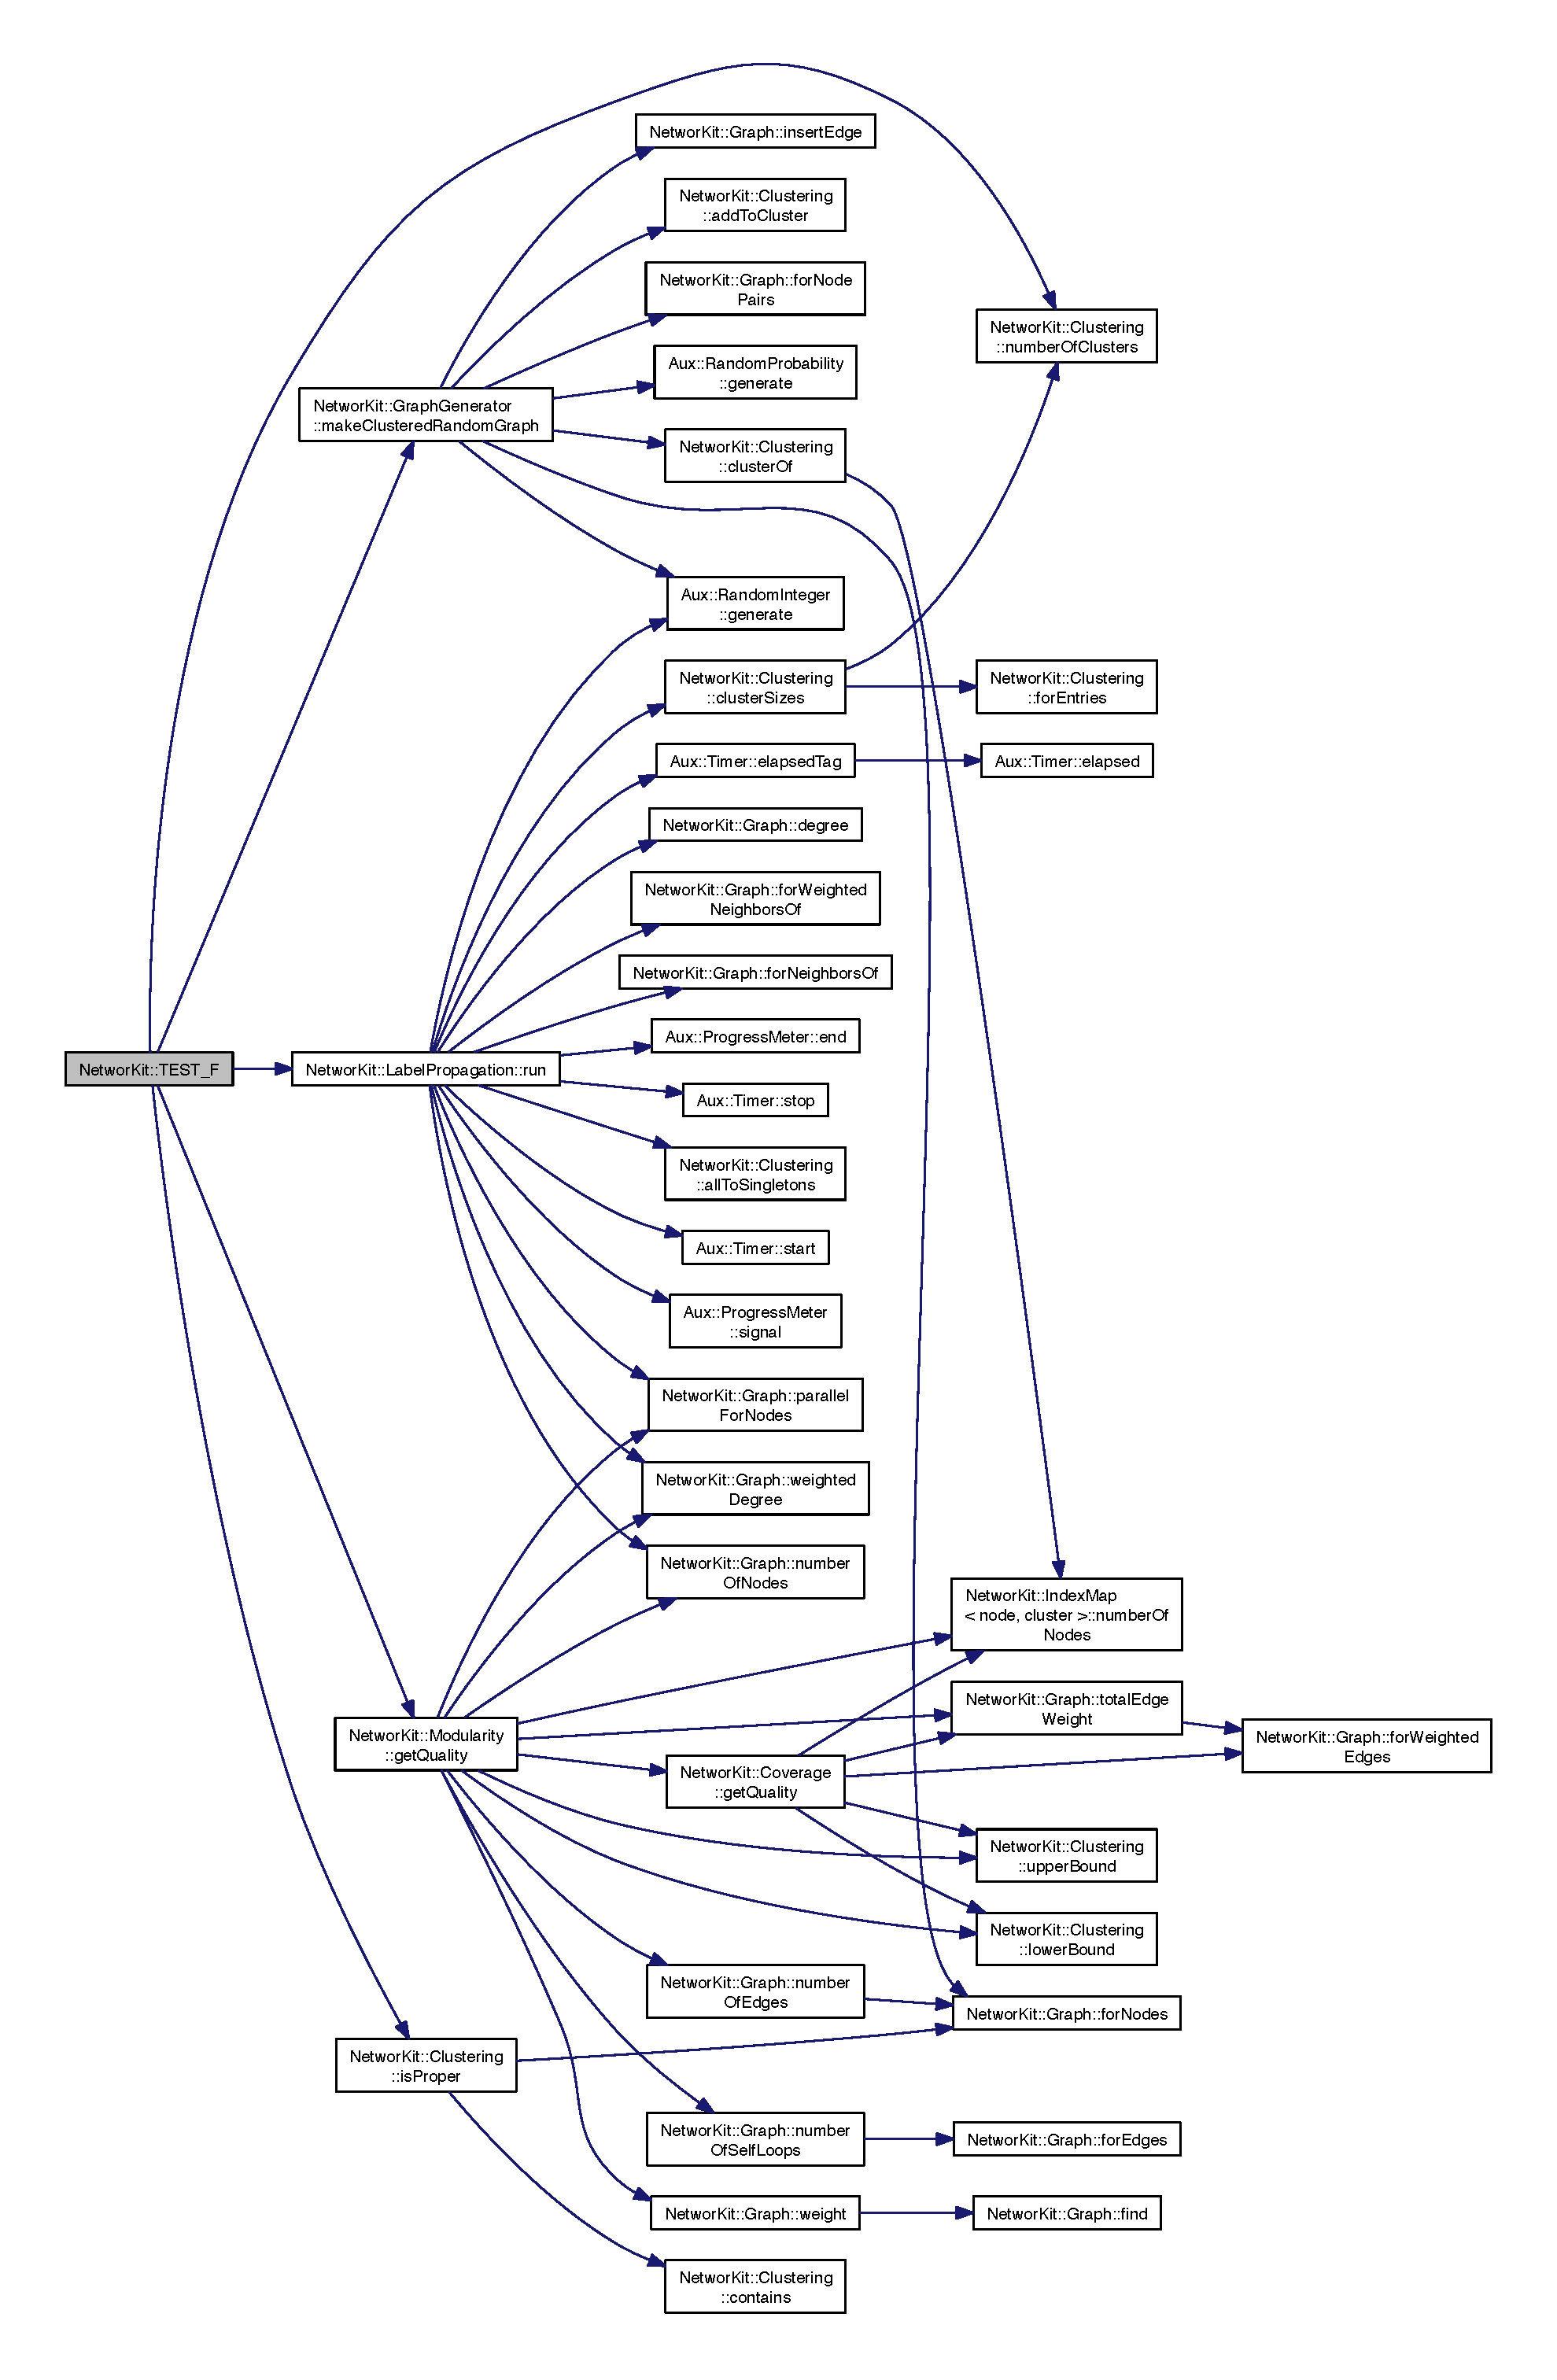
\includegraphics[width=350pt]{namespace_networ_kit_a7590ba53b3c7daa9d805db41b17d979e_cgraph}
\end{center}
\end{figure}


\hypertarget{namespace_networ_kit_a1c5826f9d4dc45c864c2cd135e7e49aa}{\index{Networ\-Kit@{Networ\-Kit}!T\-E\-S\-T\-\_\-\-F@{T\-E\-S\-T\-\_\-\-F}}
\index{T\-E\-S\-T\-\_\-\-F@{T\-E\-S\-T\-\_\-\-F}!NetworKit@{Networ\-Kit}}
\subsubsection[{T\-E\-S\-T\-\_\-\-F}]{\setlength{\rightskip}{0pt plus 5cm}Networ\-Kit\-::\-T\-E\-S\-T\-\_\-\-F (
\begin{DoxyParamCaption}
\item[{Graph2\-G\-Test}]{, }
\item[{test\-Number\-Of\-Edges}]{}
\end{DoxyParamCaption}
)}}\label{namespace_networ_kit_a1c5826f9d4dc45c864c2cd135e7e49aa}


Definition at line 32 of file Graph2\-G\-Test.\-cpp.



Here is the call graph for this function\-:\nopagebreak
\begin{figure}[H]
\begin{center}
\leavevmode
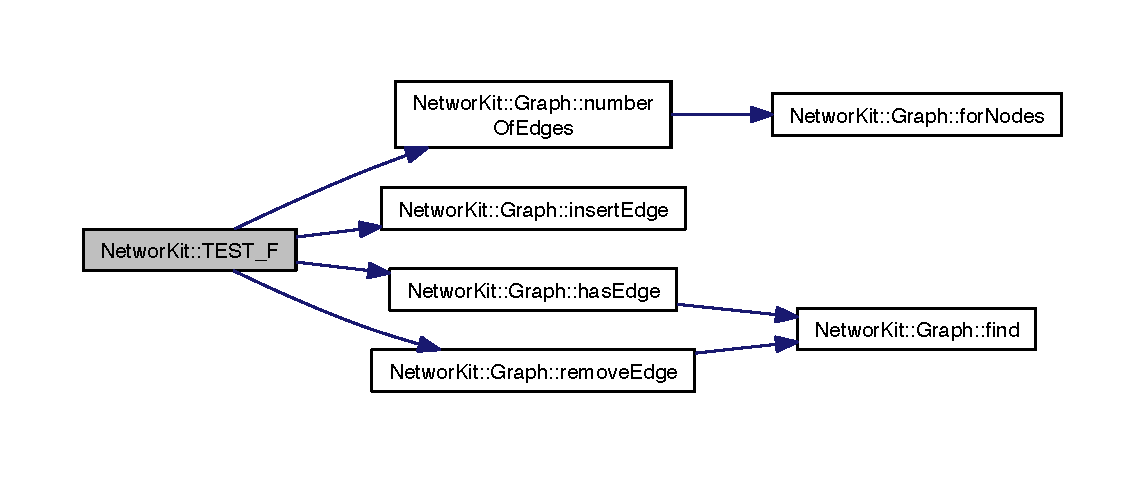
\includegraphics[width=350pt]{namespace_networ_kit_a1c5826f9d4dc45c864c2cd135e7e49aa_cgraph}
\end{center}
\end{figure}


\hypertarget{namespace_networ_kit_a0f6fd2148f725f49525424061e0d57d8}{\index{Networ\-Kit@{Networ\-Kit}!T\-E\-S\-T\-\_\-\-F@{T\-E\-S\-T\-\_\-\-F}}
\index{T\-E\-S\-T\-\_\-\-F@{T\-E\-S\-T\-\_\-\-F}!NetworKit@{Networ\-Kit}}
\subsubsection[{T\-E\-S\-T\-\_\-\-F}]{\setlength{\rightskip}{0pt plus 5cm}Networ\-Kit\-::\-T\-E\-S\-T\-\_\-\-F (
\begin{DoxyParamCaption}
\item[{Graph2\-Benchmark}]{, }
\item[{node\-Iteration}]{}
\end{DoxyParamCaption}
)}}\label{namespace_networ_kit_a0f6fd2148f725f49525424061e0d57d8}


Definition at line 35 of file Graph2\-Benchmark.\-cpp.



Here is the call graph for this function\-:\nopagebreak
\begin{figure}[H]
\begin{center}
\leavevmode
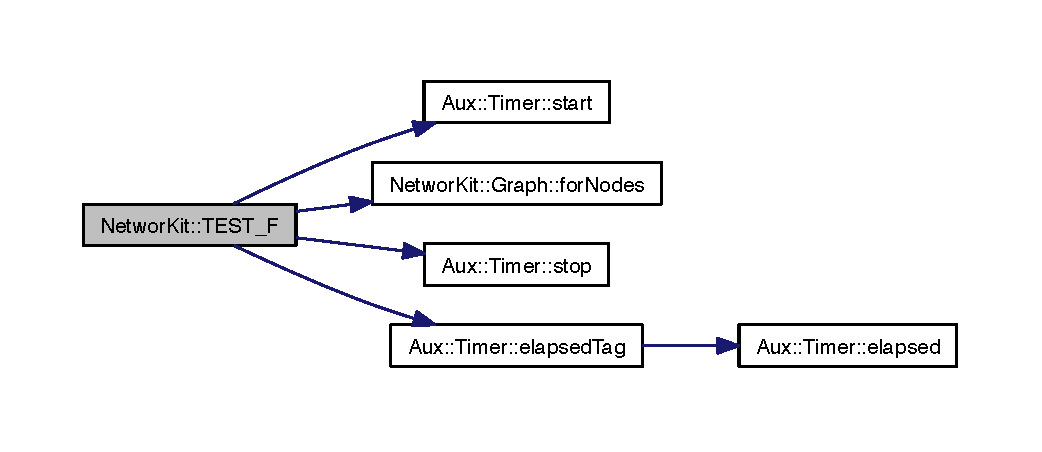
\includegraphics[width=350pt]{namespace_networ_kit_a0f6fd2148f725f49525424061e0d57d8_cgraph}
\end{center}
\end{figure}


\hypertarget{namespace_networ_kit_a12fc6da36d3dd1153a231e29b89ff862}{\index{Networ\-Kit@{Networ\-Kit}!T\-E\-S\-T\-\_\-\-F@{T\-E\-S\-T\-\_\-\-F}}
\index{T\-E\-S\-T\-\_\-\-F@{T\-E\-S\-T\-\_\-\-F}!NetworKit@{Networ\-Kit}}
\subsubsection[{T\-E\-S\-T\-\_\-\-F}]{\setlength{\rightskip}{0pt plus 5cm}Networ\-Kit\-::\-T\-E\-S\-T\-\_\-\-F (
\begin{DoxyParamCaption}
\item[{Basics\-Benchmark}]{, }
\item[{parallel\-Sum\-Incorrect}]{}
\end{DoxyParamCaption}
)}}\label{namespace_networ_kit_a12fc6da36d3dd1153a231e29b89ff862}


Definition at line 37 of file Basics\-Benchmark.\-cpp.



Here is the call graph for this function\-:\nopagebreak
\begin{figure}[H]
\begin{center}
\leavevmode
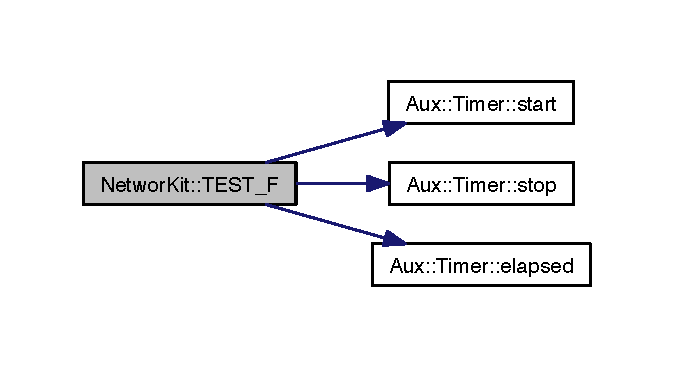
\includegraphics[width=324pt]{namespace_networ_kit_a12fc6da36d3dd1153a231e29b89ff862_cgraph}
\end{center}
\end{figure}


\hypertarget{namespace_networ_kit_aaefe3f4226eaaaa054c4e13b26822edd}{\index{Networ\-Kit@{Networ\-Kit}!T\-E\-S\-T\-\_\-\-F@{T\-E\-S\-T\-\_\-\-F}}
\index{T\-E\-S\-T\-\_\-\-F@{T\-E\-S\-T\-\_\-\-F}!NetworKit@{Networ\-Kit}}
\subsubsection[{T\-E\-S\-T\-\_\-\-F}]{\setlength{\rightskip}{0pt plus 5cm}Networ\-Kit\-::\-T\-E\-S\-T\-\_\-\-F (
\begin{DoxyParamCaption}
\item[{Coarsening\-G\-Test}]{, }
\item[{test\-Clustering\-Projector\-With\-One\-Clustering}]{}
\end{DoxyParamCaption}
)}}\label{namespace_networ_kit_aaefe3f4226eaaaa054c4e13b26822edd}


Definition at line 41 of file Coarsening\-G\-Test.\-cpp.



Here is the call graph for this function\-:\nopagebreak
\begin{figure}[H]
\begin{center}
\leavevmode
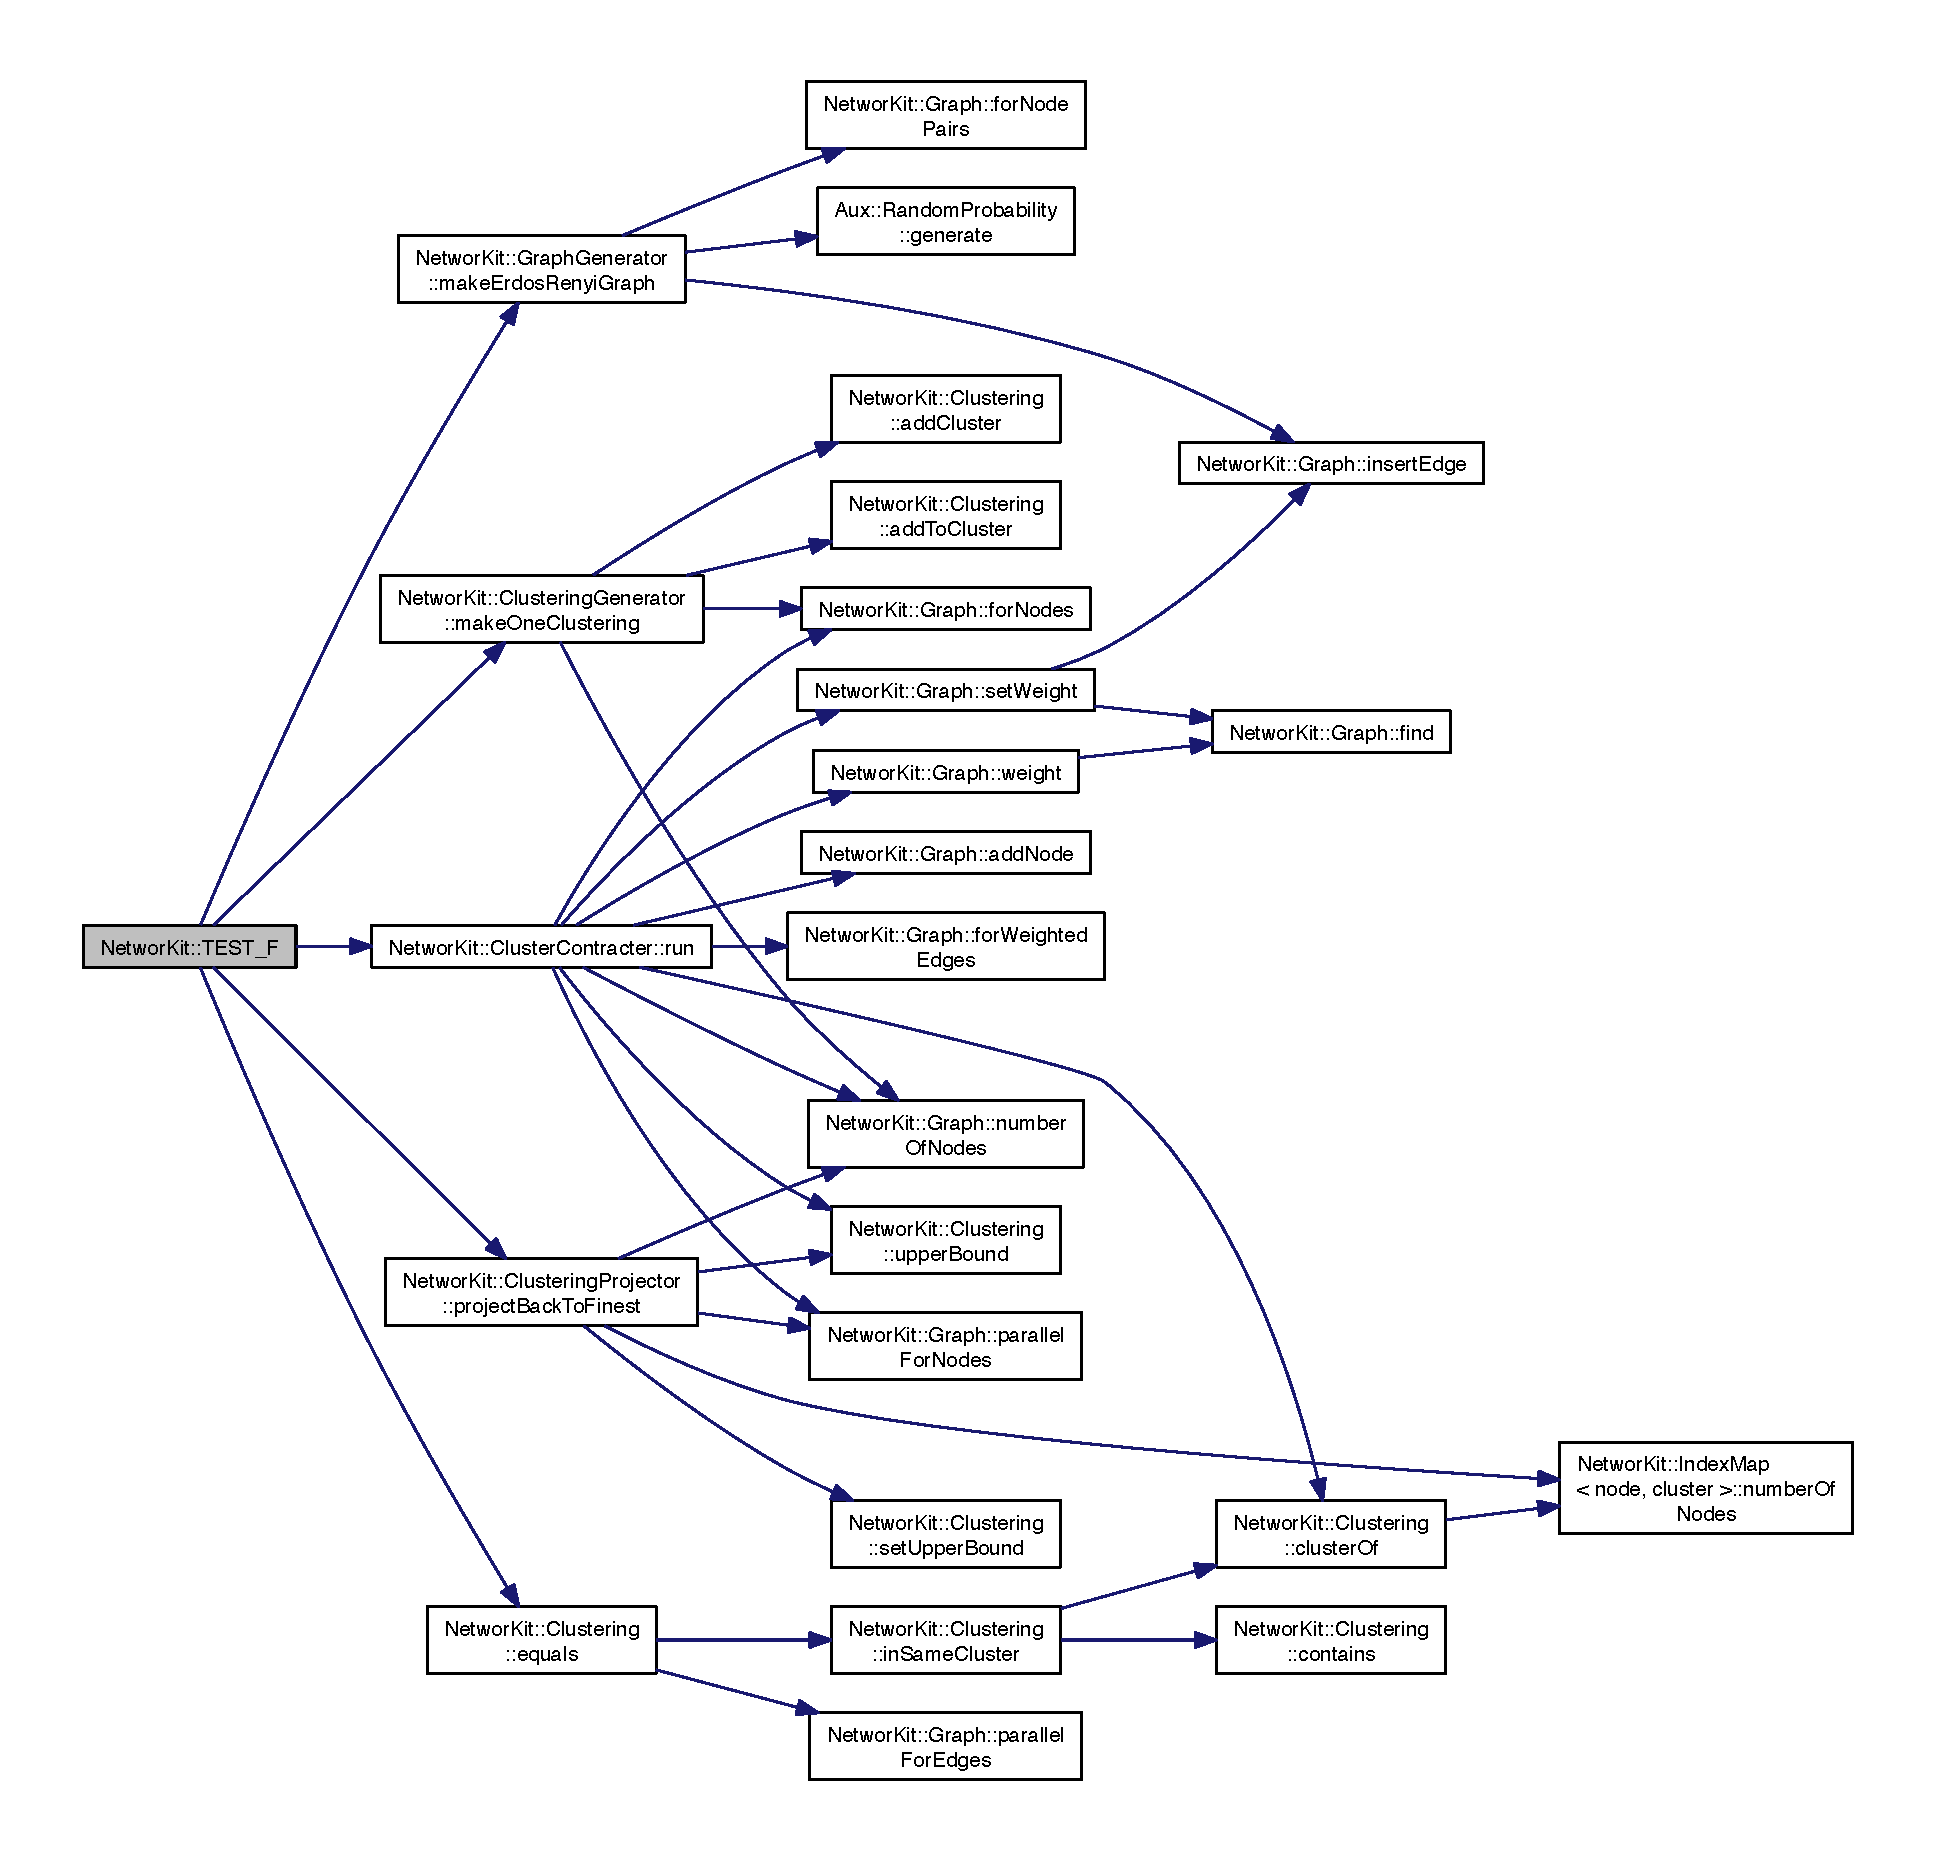
\includegraphics[width=350pt]{namespace_networ_kit_aaefe3f4226eaaaa054c4e13b26822edd_cgraph}
\end{center}
\end{figure}


\hypertarget{namespace_networ_kit_adbe4aeb718867f6f04e5f9b7c8f7cc38}{\index{Networ\-Kit@{Networ\-Kit}!T\-E\-S\-T\-\_\-\-F@{T\-E\-S\-T\-\_\-\-F}}
\index{T\-E\-S\-T\-\_\-\-F@{T\-E\-S\-T\-\_\-\-F}!NetworKit@{Networ\-Kit}}
\subsubsection[{T\-E\-S\-T\-\_\-\-F}]{\setlength{\rightskip}{0pt plus 5cm}Networ\-Kit\-::\-T\-E\-S\-T\-\_\-\-F (
\begin{DoxyParamCaption}
\item[{Independent\-Set\-G\-Test}]{, }
\item[{test\-Luby\-With\-Self\-Loops}]{}
\end{DoxyParamCaption}
)}}\label{namespace_networ_kit_adbe4aeb718867f6f04e5f9b7c8f7cc38}


Definition at line 42 of file Independent\-Set\-G\-Test.\-cpp.



Here is the call graph for this function\-:\nopagebreak
\begin{figure}[H]
\begin{center}
\leavevmode
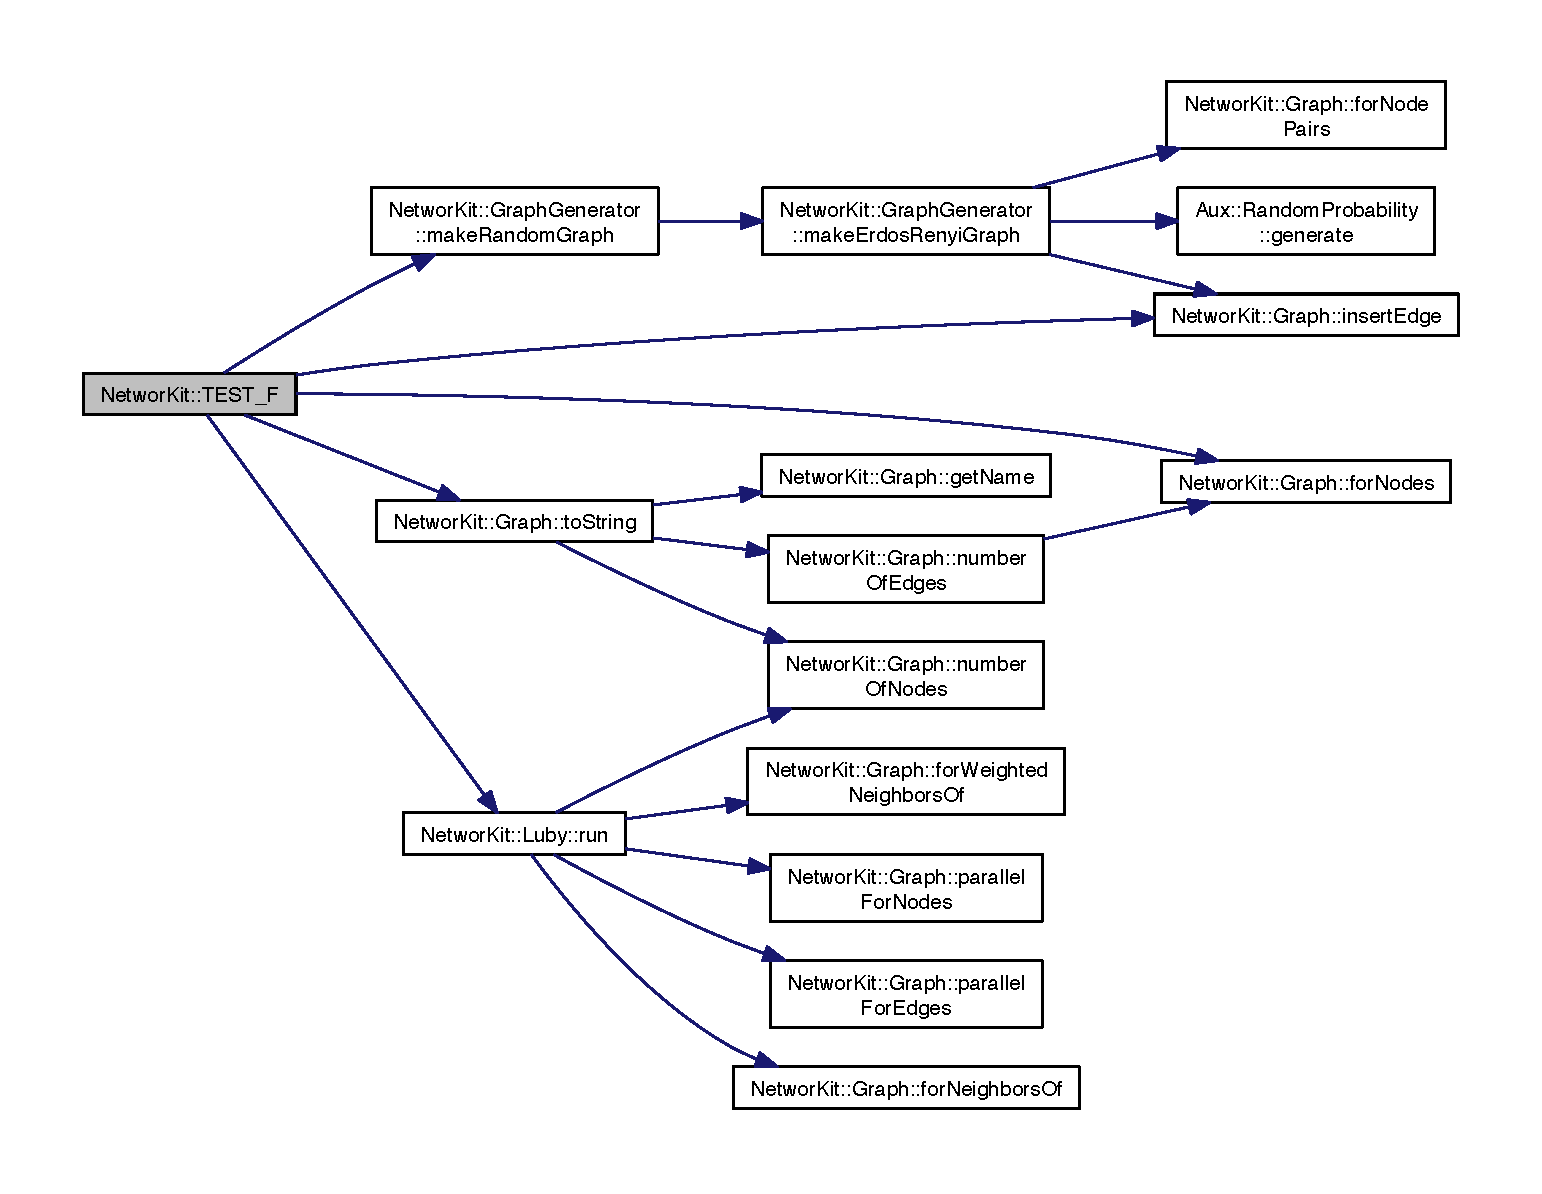
\includegraphics[width=350pt]{namespace_networ_kit_adbe4aeb718867f6f04e5f9b7c8f7cc38_cgraph}
\end{center}
\end{figure}


\hypertarget{namespace_networ_kit_a63f18361fab3ad91fc3c71f32497050b}{\index{Networ\-Kit@{Networ\-Kit}!T\-E\-S\-T\-\_\-\-F@{T\-E\-S\-T\-\_\-\-F}}
\index{T\-E\-S\-T\-\_\-\-F@{T\-E\-S\-T\-\_\-\-F}!NetworKit@{Networ\-Kit}}
\subsubsection[{T\-E\-S\-T\-\_\-\-F}]{\setlength{\rightskip}{0pt plus 5cm}Networ\-Kit\-::\-T\-E\-S\-T\-\_\-\-F (
\begin{DoxyParamCaption}
\item[{Graph\-Benchmark}]{, }
\item[{edge\-Insertions\-\_\-noop\-\_\-par}]{}
\end{DoxyParamCaption}
)}}\label{namespace_networ_kit_a63f18361fab3ad91fc3c71f32497050b}


Definition at line 43 of file Graph\-Benchmark.\-cpp.



Here is the call graph for this function\-:\nopagebreak
\begin{figure}[H]
\begin{center}
\leavevmode
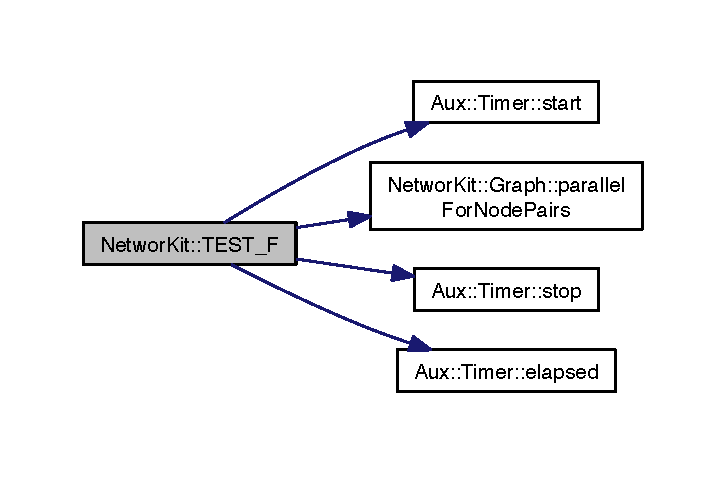
\includegraphics[width=348pt]{namespace_networ_kit_a63f18361fab3ad91fc3c71f32497050b_cgraph}
\end{center}
\end{figure}


\hypertarget{namespace_networ_kit_a2f24a06e45f75caeec4df09b75d604a8}{\index{Networ\-Kit@{Networ\-Kit}!T\-E\-S\-T\-\_\-\-F@{T\-E\-S\-T\-\_\-\-F}}
\index{T\-E\-S\-T\-\_\-\-F@{T\-E\-S\-T\-\_\-\-F}!NetworKit@{Networ\-Kit}}
\subsubsection[{T\-E\-S\-T\-\_\-\-F}]{\setlength{\rightskip}{0pt plus 5cm}Networ\-Kit\-::\-T\-E\-S\-T\-\_\-\-F (
\begin{DoxyParamCaption}
\item[{Input\-G\-Test}]{, }
\item[{test\-Graph\-I\-O\-For\-Isolated\-Nodes}]{}
\end{DoxyParamCaption}
)}}\label{namespace_networ_kit_a2f24a06e45f75caeec4df09b75d604a8}


Definition at line 43 of file Input\-G\-Test.\-cpp.



Here is the call graph for this function\-:\nopagebreak
\begin{figure}[H]
\begin{center}
\leavevmode
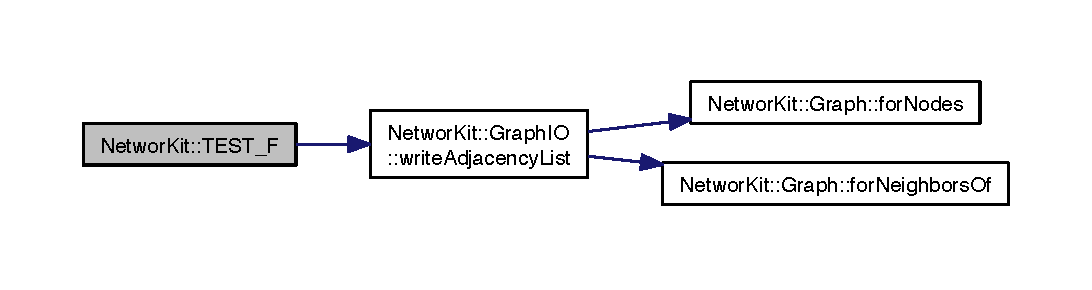
\includegraphics[width=350pt]{namespace_networ_kit_a2f24a06e45f75caeec4df09b75d604a8_cgraph}
\end{center}
\end{figure}


\hypertarget{namespace_networ_kit_a7cf6d58689907919cce6119d5a566892}{\index{Networ\-Kit@{Networ\-Kit}!T\-E\-S\-T\-\_\-\-F@{T\-E\-S\-T\-\_\-\-F}}
\index{T\-E\-S\-T\-\_\-\-F@{T\-E\-S\-T\-\_\-\-F}!NetworKit@{Networ\-Kit}}
\subsubsection[{T\-E\-S\-T\-\_\-\-F}]{\setlength{\rightskip}{0pt plus 5cm}Networ\-Kit\-::\-T\-E\-S\-T\-\_\-\-F (
\begin{DoxyParamCaption}
\item[{Overlap\-G\-Test}]{, }
\item[{test\-Region\-Growing\-Overlapper\-On\-Singleton\-Clustering}]{}
\end{DoxyParamCaption}
)}}\label{namespace_networ_kit_a7cf6d58689907919cce6119d5a566892}


Definition at line 44 of file Overlap\-G\-Test.\-cpp.



Here is the call graph for this function\-:\nopagebreak
\begin{figure}[H]
\begin{center}
\leavevmode
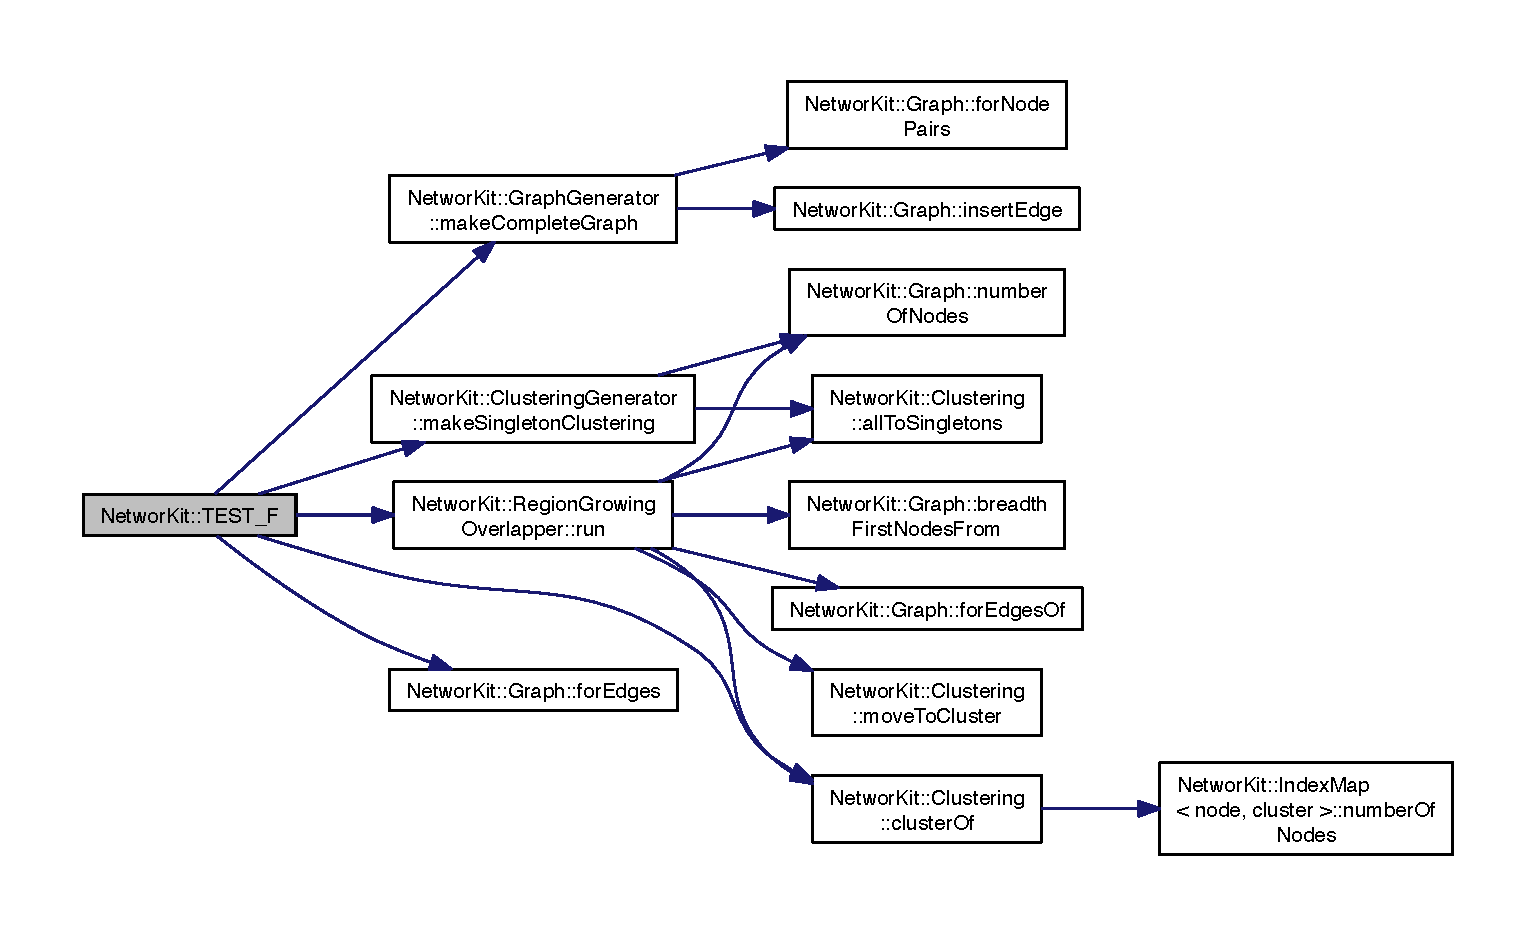
\includegraphics[width=350pt]{namespace_networ_kit_a7cf6d58689907919cce6119d5a566892_cgraph}
\end{center}
\end{figure}


\hypertarget{namespace_networ_kit_a71dcdd3a5c7565c91853184aa9f55f42}{\index{Networ\-Kit@{Networ\-Kit}!T\-E\-S\-T\-\_\-\-F@{T\-E\-S\-T\-\_\-\-F}}
\index{T\-E\-S\-T\-\_\-\-F@{T\-E\-S\-T\-\_\-\-F}!NetworKit@{Networ\-Kit}}
\subsubsection[{T\-E\-S\-T\-\_\-\-F}]{\setlength{\rightskip}{0pt plus 5cm}Networ\-Kit\-::\-T\-E\-S\-T\-\_\-\-F (
\begin{DoxyParamCaption}
\item[{Clustering\-G\-Test}]{, }
\item[{test\-Coverage}]{}
\end{DoxyParamCaption}
)}}\label{namespace_networ_kit_a71dcdd3a5c7565c91853184aa9f55f42}


Definition at line 47 of file Clustering\-G\-Test.\-cpp.



Here is the call graph for this function\-:\nopagebreak
\begin{figure}[H]
\begin{center}
\leavevmode
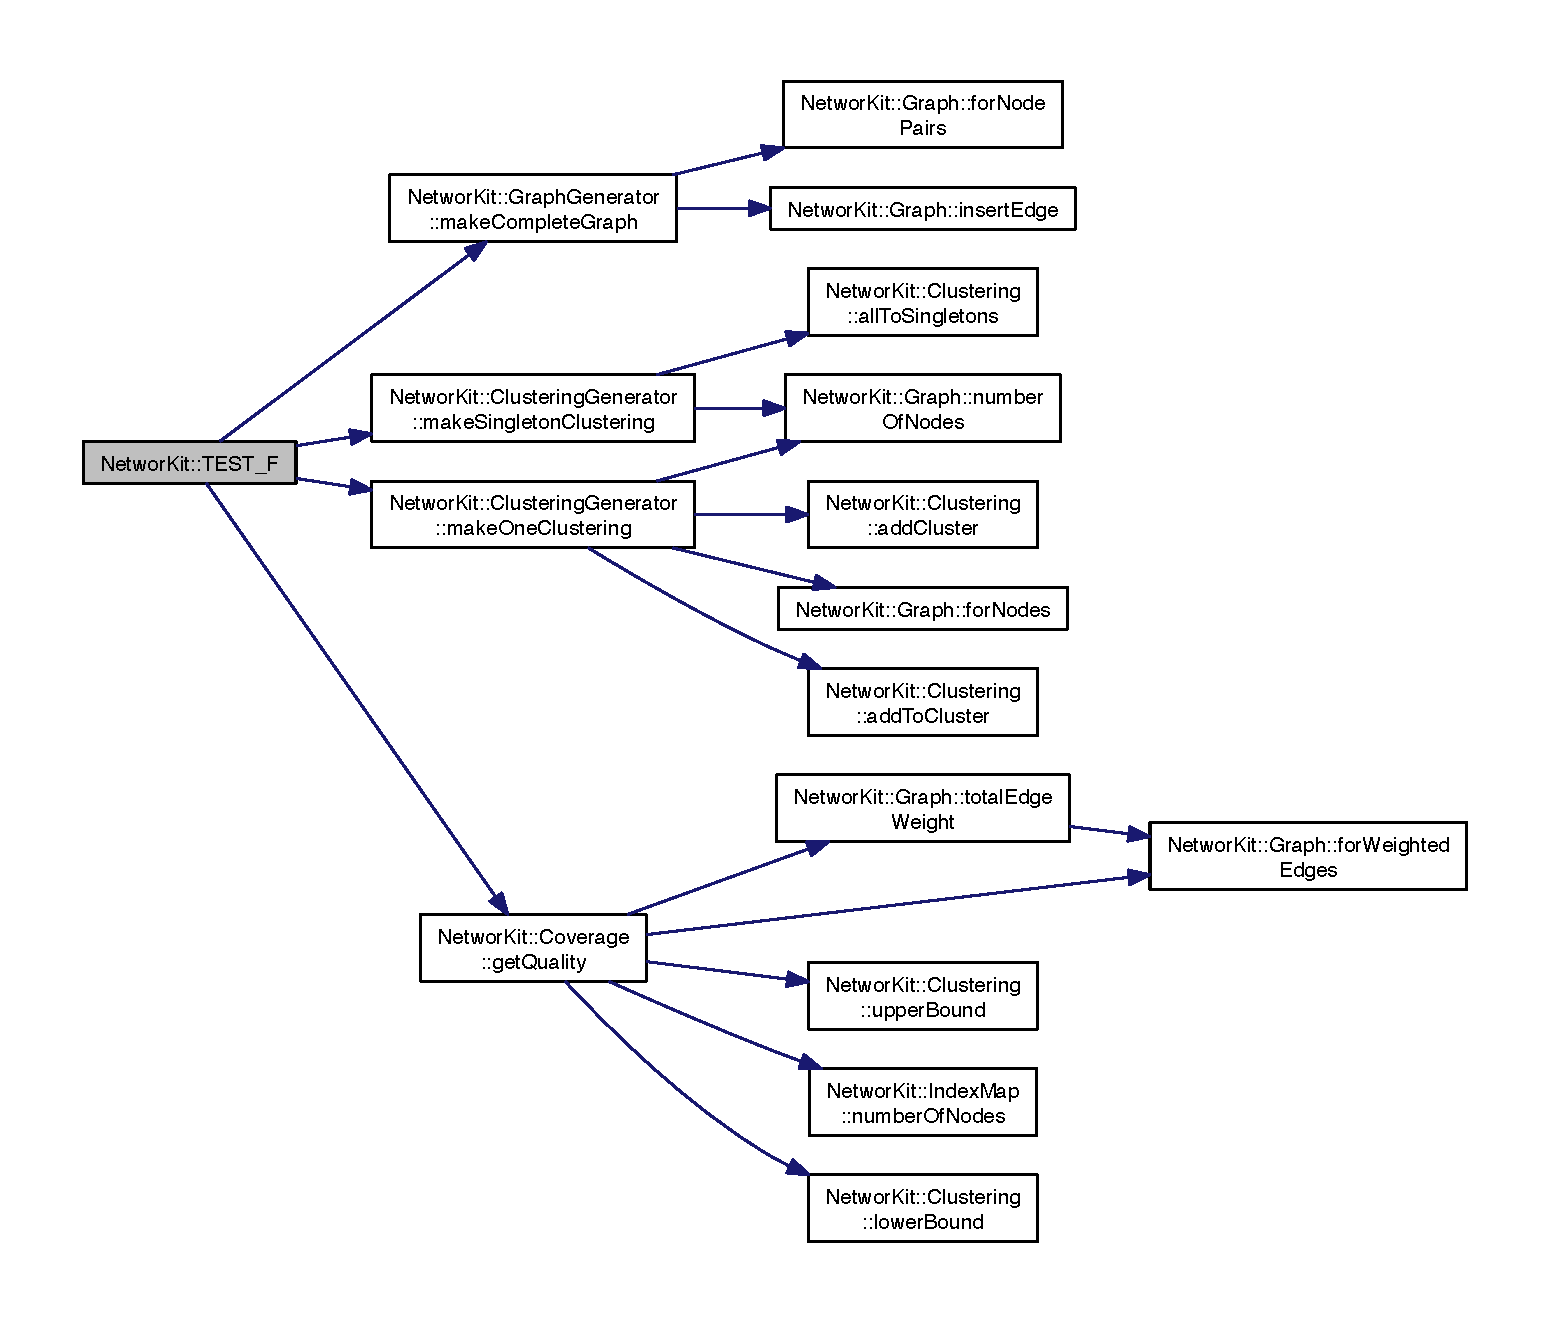
\includegraphics[width=350pt]{namespace_networ_kit_a71dcdd3a5c7565c91853184aa9f55f42_cgraph}
\end{center}
\end{figure}


\hypertarget{namespace_networ_kit_a2ec052386a15b77a9da5452d6866aa60}{\index{Networ\-Kit@{Networ\-Kit}!T\-E\-S\-T\-\_\-\-F@{T\-E\-S\-T\-\_\-\-F}}
\index{T\-E\-S\-T\-\_\-\-F@{T\-E\-S\-T\-\_\-\-F}!NetworKit@{Networ\-Kit}}
\subsubsection[{T\-E\-S\-T\-\_\-\-F}]{\setlength{\rightskip}{0pt plus 5cm}Networ\-Kit\-::\-T\-E\-S\-T\-\_\-\-F (
\begin{DoxyParamCaption}
\item[{Graph\-G\-Test}]{, }
\item[{test\-Parallel\-Lambda\-Edge\-Iteration}]{}
\end{DoxyParamCaption}
)}}\label{namespace_networ_kit_a2ec052386a15b77a9da5452d6866aa60}


Definition at line 47 of file Graph\-G\-Test.\-cpp.



Here is the call graph for this function\-:\nopagebreak
\begin{figure}[H]
\begin{center}
\leavevmode
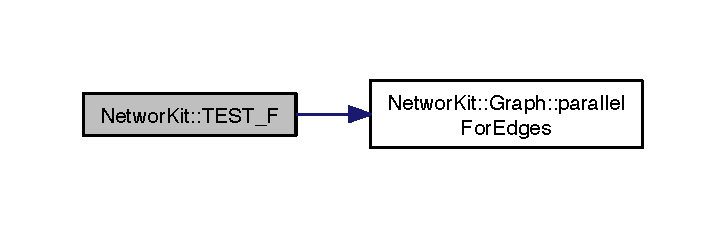
\includegraphics[width=348pt]{namespace_networ_kit_a2ec052386a15b77a9da5452d6866aa60_cgraph}
\end{center}
\end{figure}


\hypertarget{namespace_networ_kit_a47440ebf4f9b819ed49f7d43584fcafa}{\index{Networ\-Kit@{Networ\-Kit}!T\-E\-S\-T\-\_\-\-F@{T\-E\-S\-T\-\_\-\-F}}
\index{T\-E\-S\-T\-\_\-\-F@{T\-E\-S\-T\-\_\-\-F}!NetworKit@{Networ\-Kit}}
\subsubsection[{T\-E\-S\-T\-\_\-\-F}]{\setlength{\rightskip}{0pt plus 5cm}Networ\-Kit\-::\-T\-E\-S\-T\-\_\-\-F (
\begin{DoxyParamCaption}
\item[{Clustering\-Algo\-G\-Test}]{, }
\item[{test\-Label\-Propagation\-On\-Clustered\-Graph\-\_\-\-For\-Equality}]{}
\end{DoxyParamCaption}
)}}\label{namespace_networ_kit_a47440ebf4f9b819ed49f7d43584fcafa}


Definition at line 49 of file Clustering\-Algo\-G\-Test.\-cpp.



Here is the call graph for this function\-:\nopagebreak
\begin{figure}[H]
\begin{center}
\leavevmode
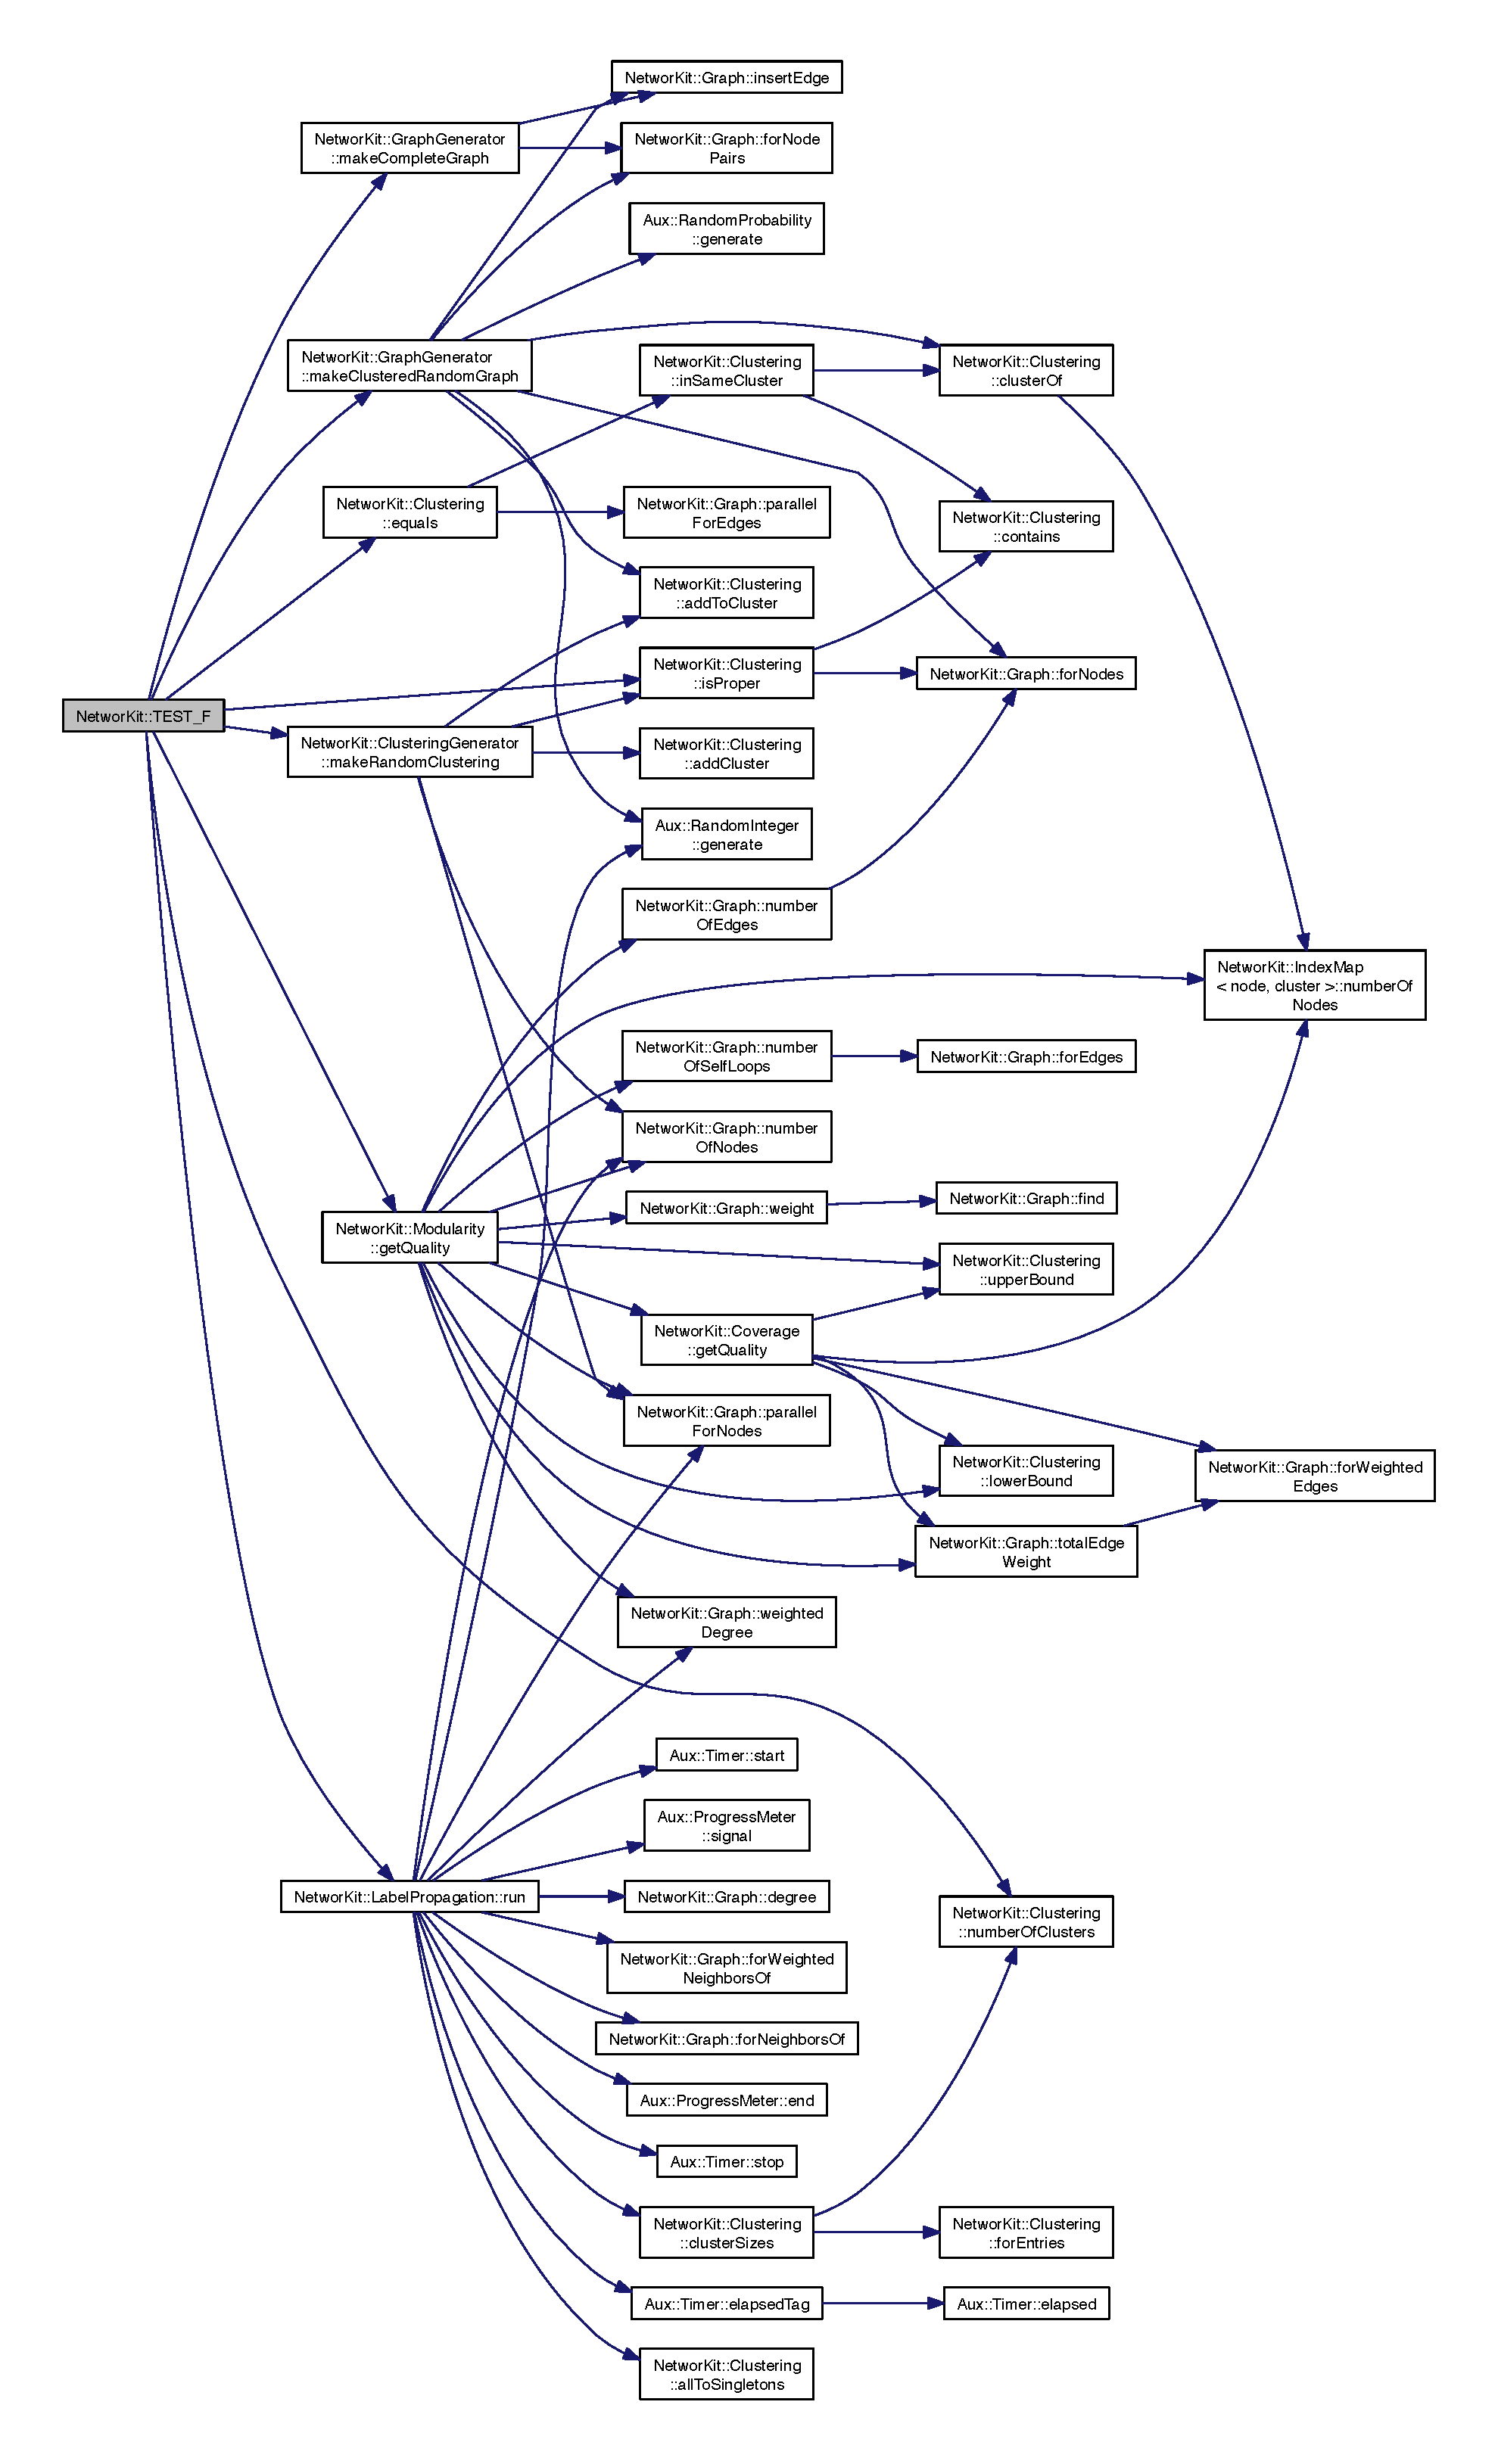
\includegraphics[height=550pt]{namespace_networ_kit_a47440ebf4f9b819ed49f7d43584fcafa_cgraph}
\end{center}
\end{figure}


\hypertarget{namespace_networ_kit_afc036b6f174e2b06a52aca2d4b10d7de}{\index{Networ\-Kit@{Networ\-Kit}!T\-E\-S\-T\-\_\-\-F@{T\-E\-S\-T\-\_\-\-F}}
\index{T\-E\-S\-T\-\_\-\-F@{T\-E\-S\-T\-\_\-\-F}!NetworKit@{Networ\-Kit}}
\subsubsection[{T\-E\-S\-T\-\_\-\-F}]{\setlength{\rightskip}{0pt plus 5cm}Networ\-Kit\-::\-T\-E\-S\-T\-\_\-\-F (
\begin{DoxyParamCaption}
\item[{Basics\-Benchmark}]{, }
\item[{parallel\-Sum\-Atomic\-Update}]{}
\end{DoxyParamCaption}
)}}\label{namespace_networ_kit_afc036b6f174e2b06a52aca2d4b10d7de}


Definition at line 52 of file Basics\-Benchmark.\-cpp.



Here is the call graph for this function\-:\nopagebreak
\begin{figure}[H]
\begin{center}
\leavevmode
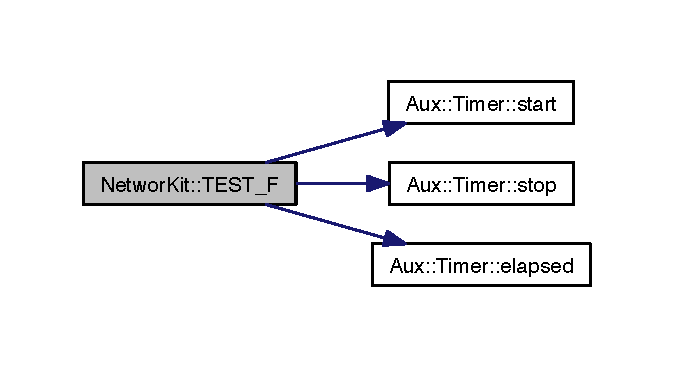
\includegraphics[width=324pt]{namespace_networ_kit_afc036b6f174e2b06a52aca2d4b10d7de_cgraph}
\end{center}
\end{figure}


\hypertarget{namespace_networ_kit_a021d1e9c1f29871187483f76919e1898}{\index{Networ\-Kit@{Networ\-Kit}!T\-E\-S\-T\-\_\-\-F@{T\-E\-S\-T\-\_\-\-F}}
\index{T\-E\-S\-T\-\_\-\-F@{T\-E\-S\-T\-\_\-\-F}!NetworKit@{Networ\-Kit}}
\subsubsection[{T\-E\-S\-T\-\_\-\-F}]{\setlength{\rightskip}{0pt plus 5cm}Networ\-Kit\-::\-T\-E\-S\-T\-\_\-\-F (
\begin{DoxyParamCaption}
\item[{Graph2\-Benchmark}]{, }
\item[{parallel\-Node\-Iteration}]{}
\end{DoxyParamCaption}
)}}\label{namespace_networ_kit_a021d1e9c1f29871187483f76919e1898}


Definition at line 55 of file Graph2\-Benchmark.\-cpp.



Here is the call graph for this function\-:\nopagebreak
\begin{figure}[H]
\begin{center}
\leavevmode
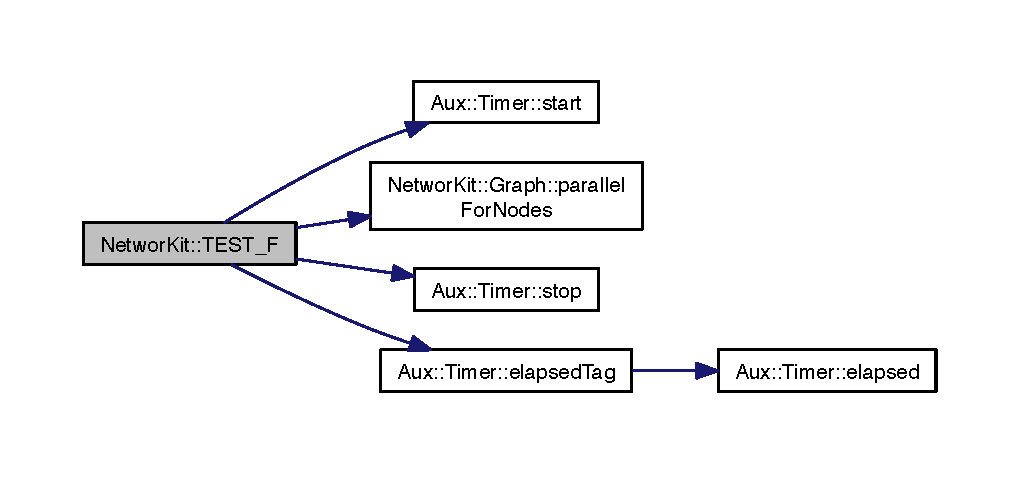
\includegraphics[width=350pt]{namespace_networ_kit_a021d1e9c1f29871187483f76919e1898_cgraph}
\end{center}
\end{figure}


\hypertarget{namespace_networ_kit_a5c7ec10a80327d1f725240dd250447cb}{\index{Networ\-Kit@{Networ\-Kit}!T\-E\-S\-T\-\_\-\-F@{T\-E\-S\-T\-\_\-\-F}}
\index{T\-E\-S\-T\-\_\-\-F@{T\-E\-S\-T\-\_\-\-F}!NetworKit@{Networ\-Kit}}
\subsubsection[{T\-E\-S\-T\-\_\-\-F}]{\setlength{\rightskip}{0pt plus 5cm}Networ\-Kit\-::\-T\-E\-S\-T\-\_\-\-F (
\begin{DoxyParamCaption}
\item[{Graph2\-G\-Test}]{, }
\item[{test\-Is\-Empty}]{}
\end{DoxyParamCaption}
)}}\label{namespace_networ_kit_a5c7ec10a80327d1f725240dd250447cb}


Definition at line 57 of file Graph2\-G\-Test.\-cpp.



Here is the call graph for this function\-:\nopagebreak
\begin{figure}[H]
\begin{center}
\leavevmode
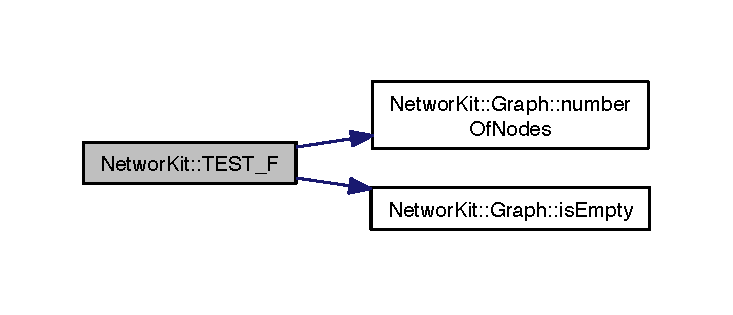
\includegraphics[width=350pt]{namespace_networ_kit_a5c7ec10a80327d1f725240dd250447cb_cgraph}
\end{center}
\end{figure}


\hypertarget{namespace_networ_kit_a36ec61ec5bc474b3725ed82139d9baaa}{\index{Networ\-Kit@{Networ\-Kit}!T\-E\-S\-T\-\_\-\-F@{T\-E\-S\-T\-\_\-\-F}}
\index{T\-E\-S\-T\-\_\-\-F@{T\-E\-S\-T\-\_\-\-F}!NetworKit@{Networ\-Kit}}
\subsubsection[{T\-E\-S\-T\-\_\-\-F}]{\setlength{\rightskip}{0pt plus 5cm}Networ\-Kit\-::\-T\-E\-S\-T\-\_\-\-F (
\begin{DoxyParamCaption}
\item[{Input\-G\-Test}]{, }
\item[{test\-M\-E\-T\-I\-S\-Graph\-Reader}]{}
\end{DoxyParamCaption}
)}}\label{namespace_networ_kit_a36ec61ec5bc474b3725ed82139d9baaa}


Definition at line 60 of file Input\-G\-Test.\-cpp.



Here is the call graph for this function\-:\nopagebreak
\begin{figure}[H]
\begin{center}
\leavevmode
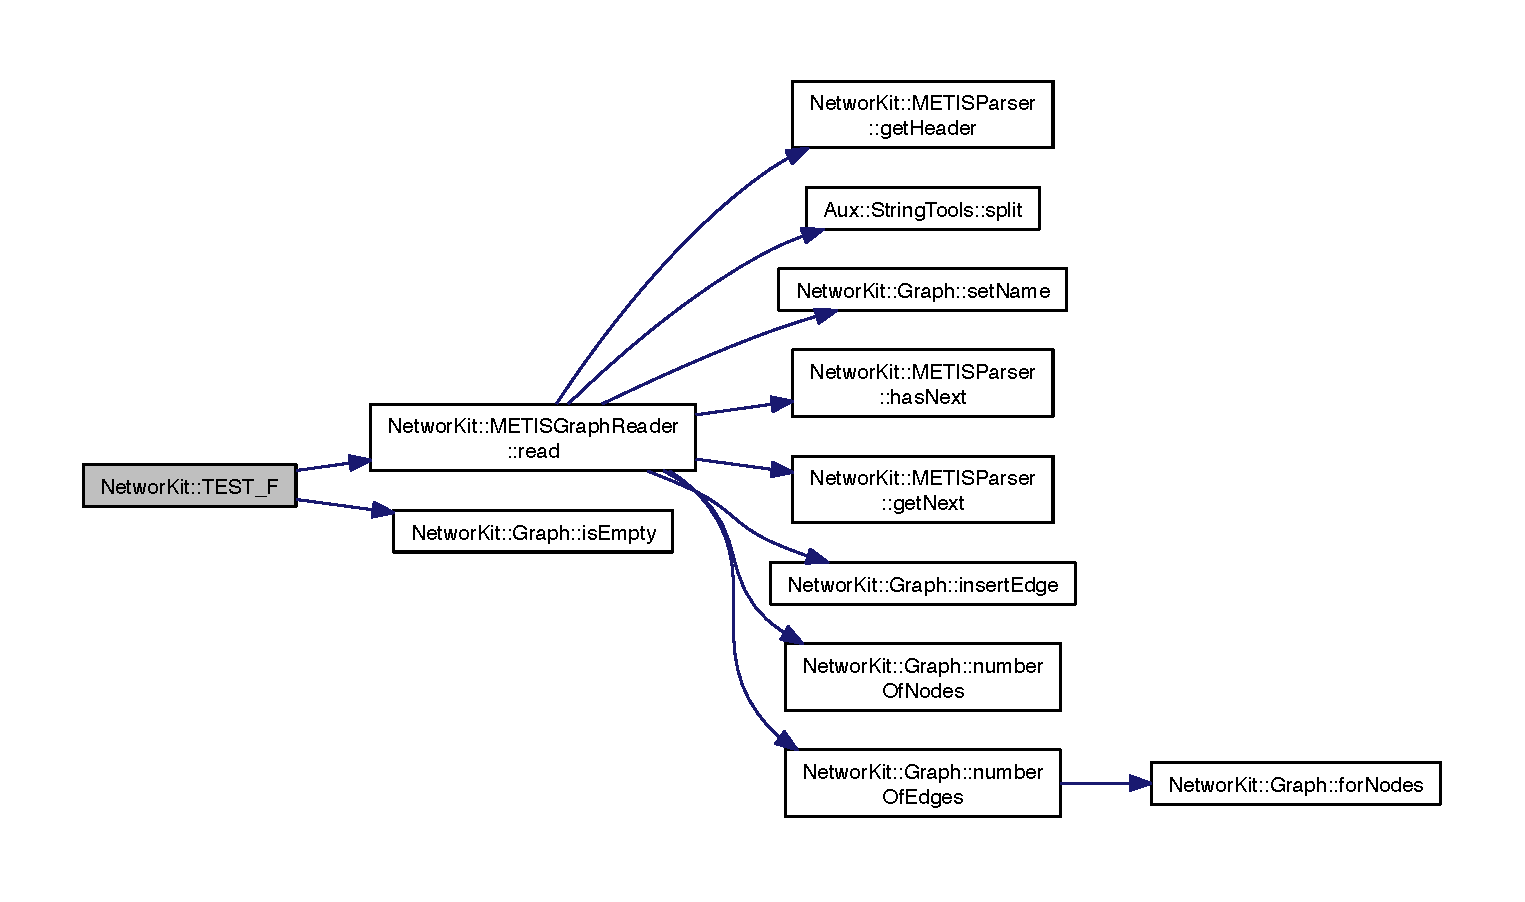
\includegraphics[width=350pt]{namespace_networ_kit_a36ec61ec5bc474b3725ed82139d9baaa_cgraph}
\end{center}
\end{figure}


\hypertarget{namespace_networ_kit_a8c65560bd7dca56d87f0f6fb4711e380}{\index{Networ\-Kit@{Networ\-Kit}!T\-E\-S\-T\-\_\-\-F@{T\-E\-S\-T\-\_\-\-F}}
\index{T\-E\-S\-T\-\_\-\-F@{T\-E\-S\-T\-\_\-\-F}!NetworKit@{Networ\-Kit}}
\subsubsection[{T\-E\-S\-T\-\_\-\-F}]{\setlength{\rightskip}{0pt plus 5cm}Networ\-Kit\-::\-T\-E\-S\-T\-\_\-\-F (
\begin{DoxyParamCaption}
\item[{Graph\-Benchmark}]{, }
\item[{edge\-Insertions\-\_\-standard\-\_\-seq}]{}
\end{DoxyParamCaption}
)}}\label{namespace_networ_kit_a8c65560bd7dca56d87f0f6fb4711e380}


Definition at line 62 of file Graph\-Benchmark.\-cpp.



Here is the call graph for this function\-:\nopagebreak
\begin{figure}[H]
\begin{center}
\leavevmode
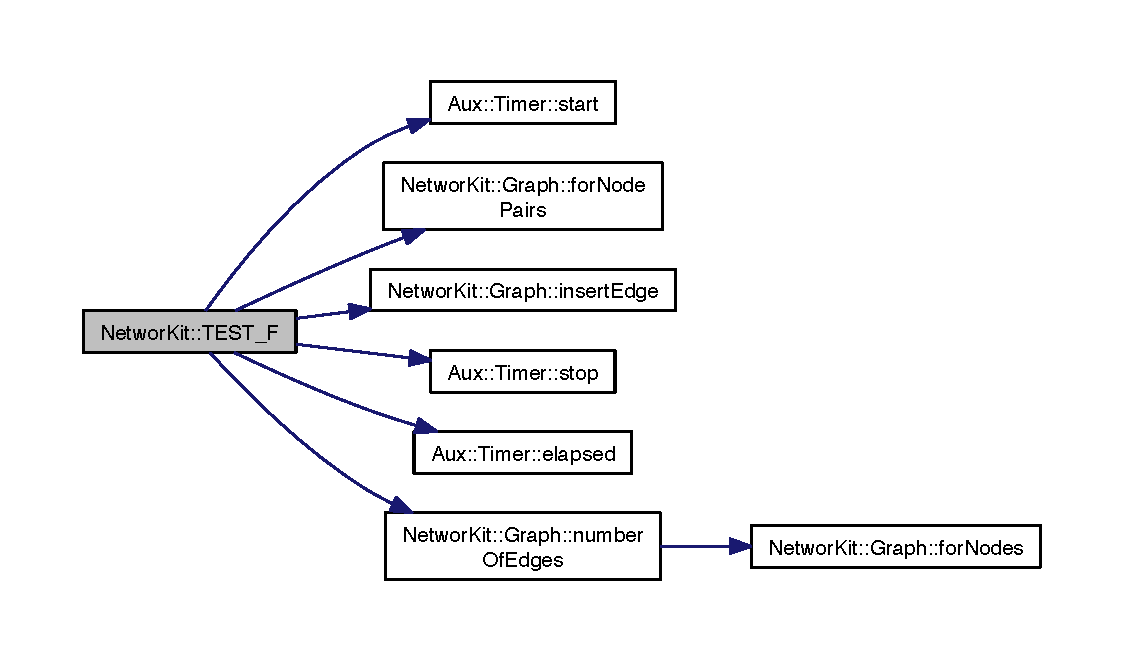
\includegraphics[width=350pt]{namespace_networ_kit_a8c65560bd7dca56d87f0f6fb4711e380_cgraph}
\end{center}
\end{figure}


\hypertarget{namespace_networ_kit_a1ec91cf47d849707d2972eabe5a98e5b}{\index{Networ\-Kit@{Networ\-Kit}!T\-E\-S\-T\-\_\-\-F@{T\-E\-S\-T\-\_\-\-F}}
\index{T\-E\-S\-T\-\_\-\-F@{T\-E\-S\-T\-\_\-\-F}!NetworKit@{Networ\-Kit}}
\subsubsection[{T\-E\-S\-T\-\_\-\-F}]{\setlength{\rightskip}{0pt plus 5cm}Networ\-Kit\-::\-T\-E\-S\-T\-\_\-\-F (
\begin{DoxyParamCaption}
\item[{Ensemble\-G\-Test}]{, }
\item[{test\-Ensemble\-Clusterer\-On\-Clique\-Graph\-\_\-\-Many\-Base\-Clusterers}]{}
\end{DoxyParamCaption}
)}}\label{namespace_networ_kit_a1ec91cf47d849707d2972eabe5a98e5b}


Definition at line 63 of file Ensemble\-G\-Test.\-cpp.



Here is the call graph for this function\-:\nopagebreak
\begin{figure}[H]
\begin{center}
\leavevmode
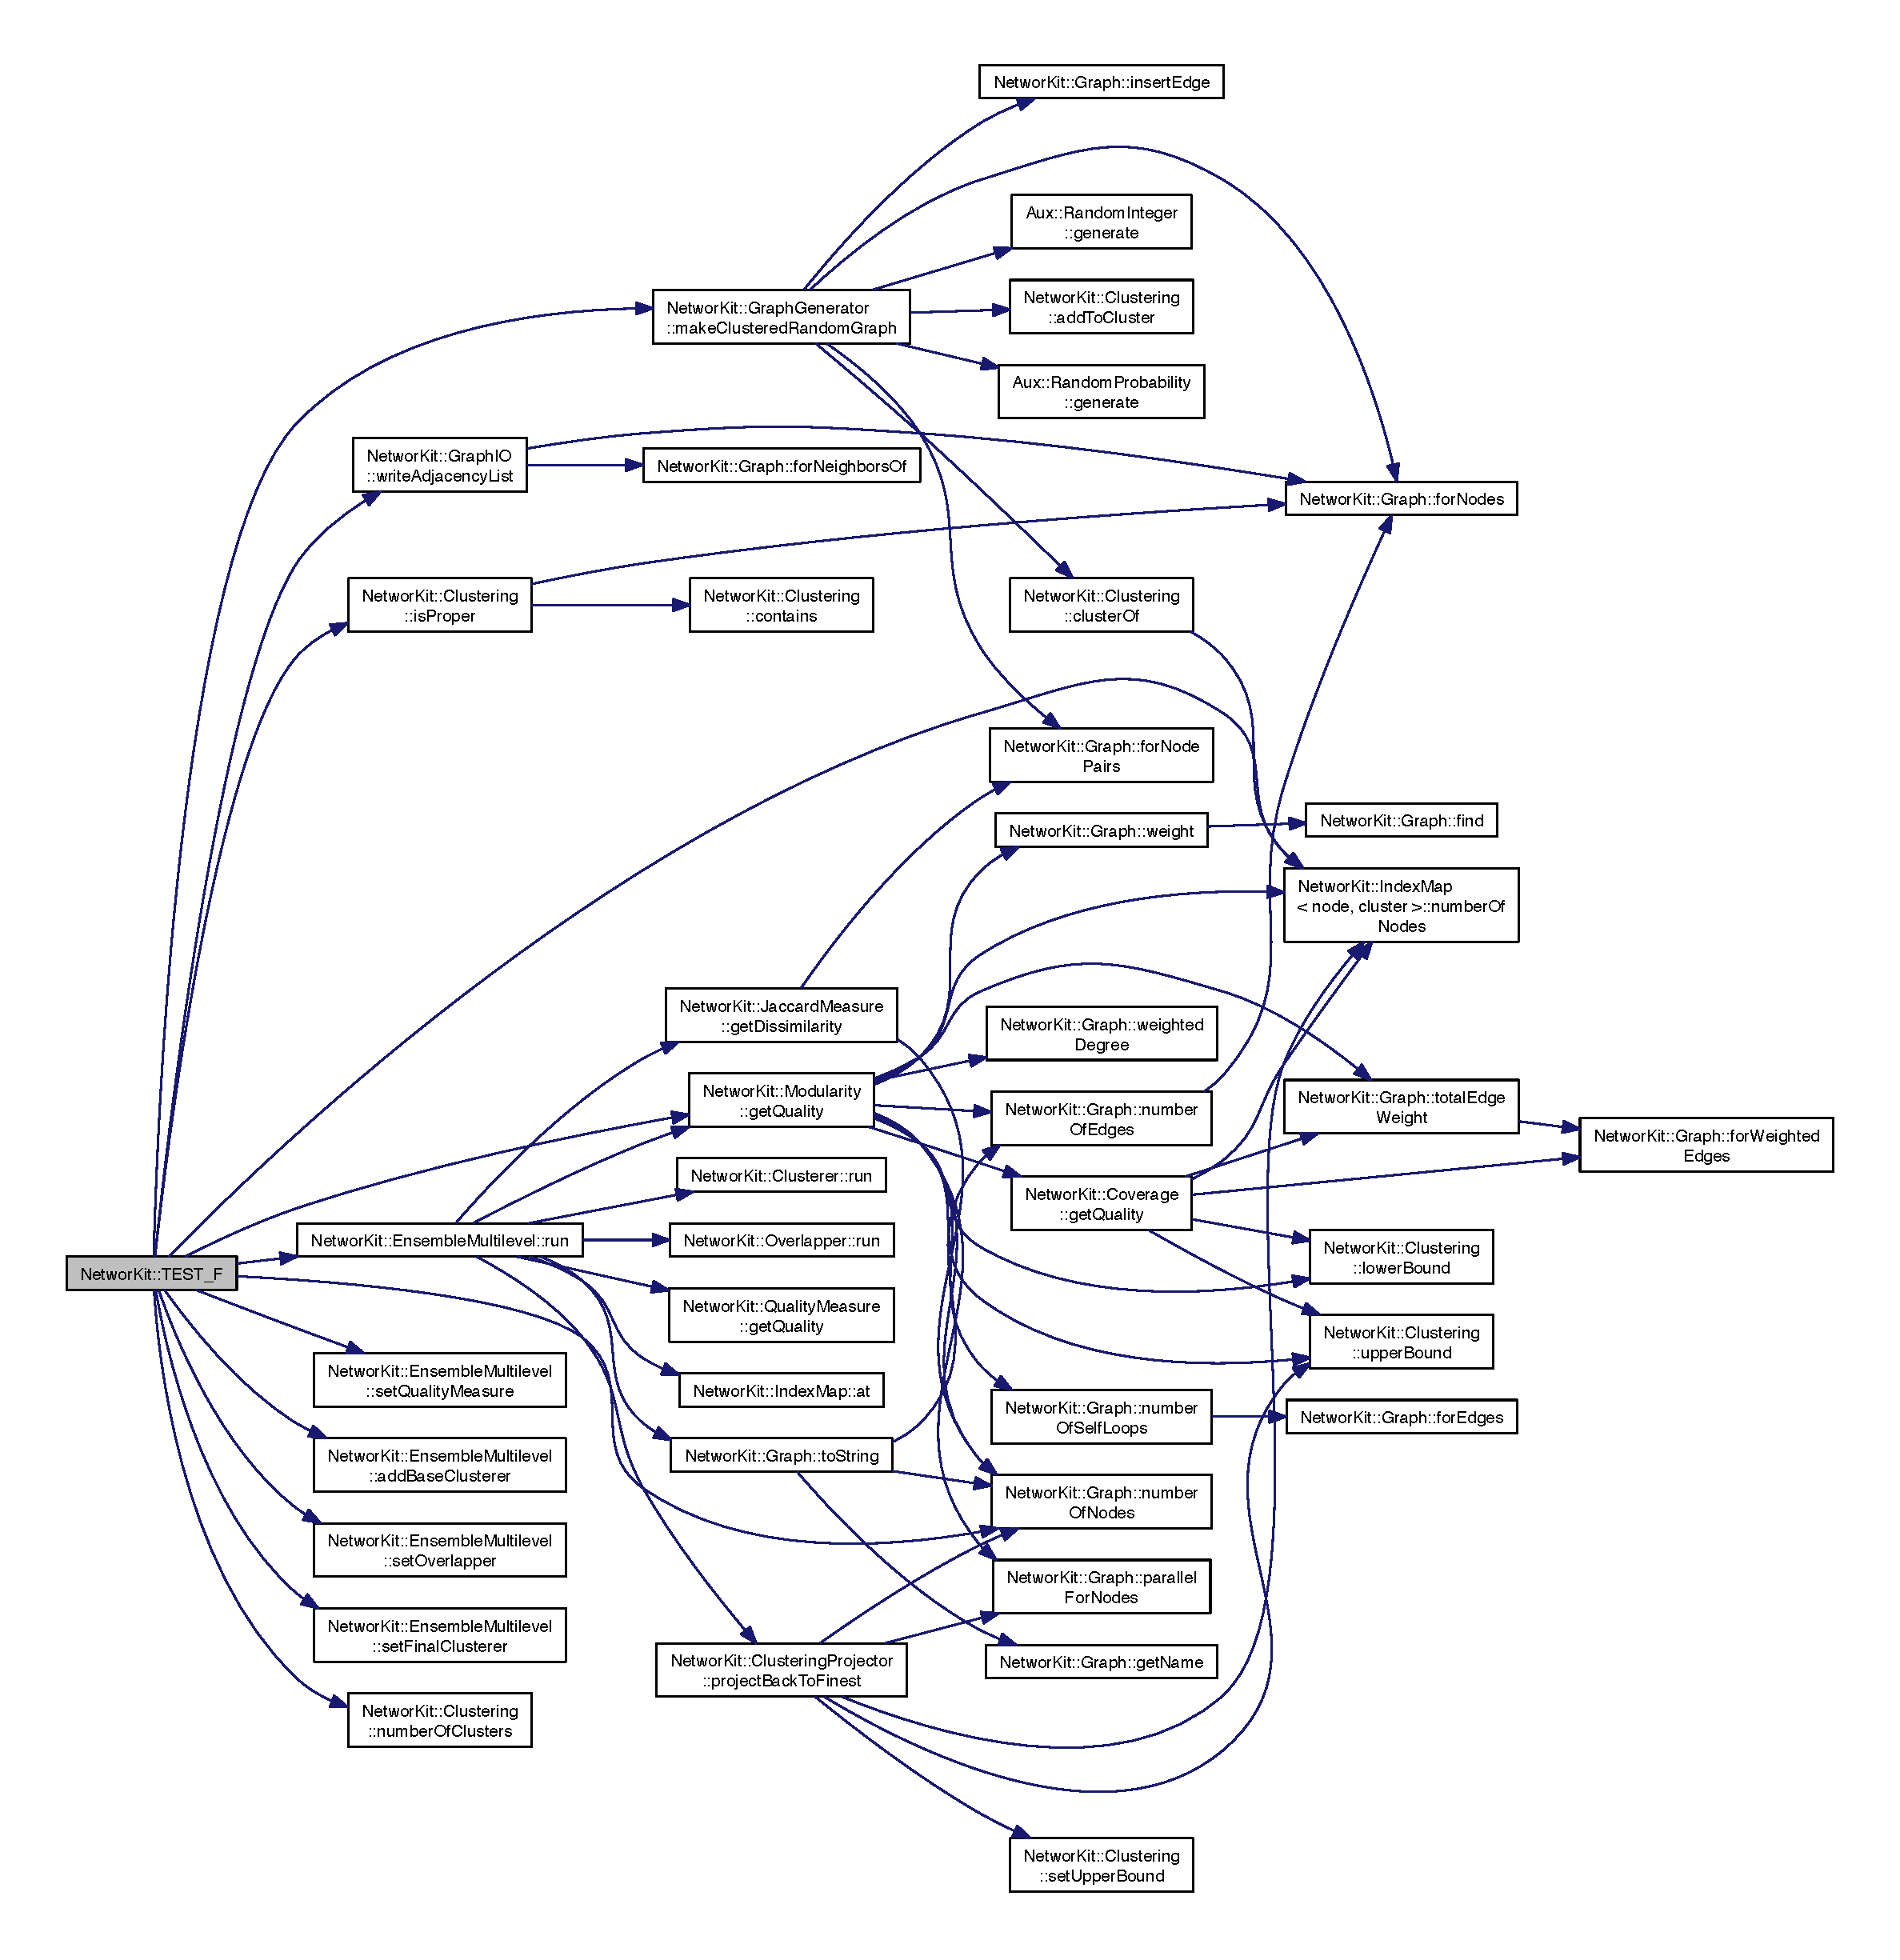
\includegraphics[width=350pt]{namespace_networ_kit_a1ec91cf47d849707d2972eabe5a98e5b_cgraph}
\end{center}
\end{figure}


\hypertarget{namespace_networ_kit_a15c2af1f595eb5507495a3d3a6cb88e5}{\index{Networ\-Kit@{Networ\-Kit}!T\-E\-S\-T\-\_\-\-F@{T\-E\-S\-T\-\_\-\-F}}
\index{T\-E\-S\-T\-\_\-\-F@{T\-E\-S\-T\-\_\-\-F}!NetworKit@{Networ\-Kit}}
\subsubsection[{T\-E\-S\-T\-\_\-\-F}]{\setlength{\rightskip}{0pt plus 5cm}Networ\-Kit\-::\-T\-E\-S\-T\-\_\-\-F (
\begin{DoxyParamCaption}
\item[{Graph2\-G\-Test}]{, }
\item[{test\-Edge\-Insertion\-And\-Removal}]{}
\end{DoxyParamCaption}
)}}\label{namespace_networ_kit_a15c2af1f595eb5507495a3d3a6cb88e5}


Definition at line 65 of file Graph2\-G\-Test.\-cpp.



Here is the call graph for this function\-:\nopagebreak
\begin{figure}[H]
\begin{center}
\leavevmode
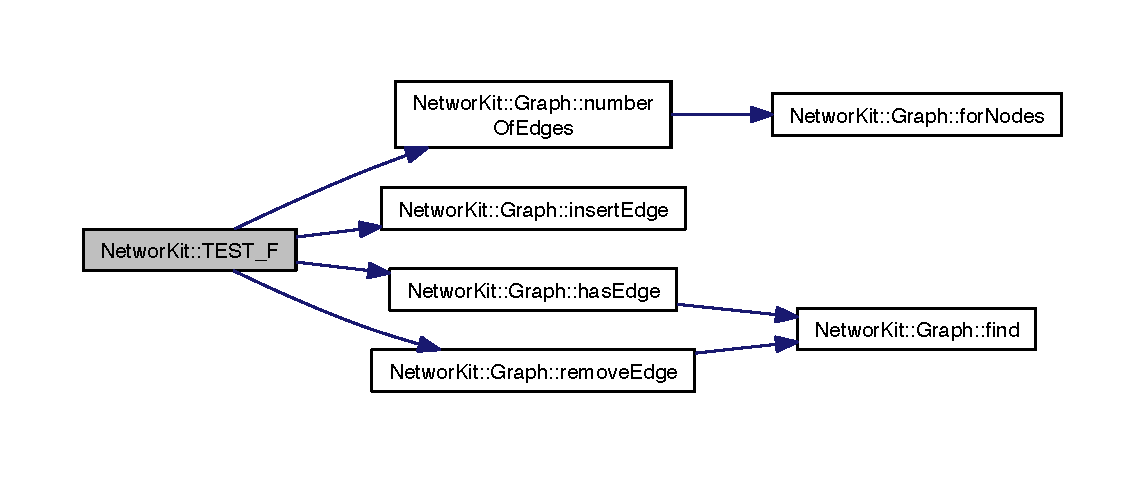
\includegraphics[width=350pt]{namespace_networ_kit_a15c2af1f595eb5507495a3d3a6cb88e5_cgraph}
\end{center}
\end{figure}


\hypertarget{namespace_networ_kit_ae1c2725eb57fbfe2f0d42512d453d70a}{\index{Networ\-Kit@{Networ\-Kit}!T\-E\-S\-T\-\_\-\-F@{T\-E\-S\-T\-\_\-\-F}}
\index{T\-E\-S\-T\-\_\-\-F@{T\-E\-S\-T\-\_\-\-F}!NetworKit@{Networ\-Kit}}
\subsubsection[{T\-E\-S\-T\-\_\-\-F}]{\setlength{\rightskip}{0pt plus 5cm}Networ\-Kit\-::\-T\-E\-S\-T\-\_\-\-F (
\begin{DoxyParamCaption}
\item[{Graph\-G\-Test}]{, }
\item[{test\-Lambda\-Edge\-Modification}]{}
\end{DoxyParamCaption}
)}}\label{namespace_networ_kit_ae1c2725eb57fbfe2f0d42512d453d70a}


Definition at line 66 of file Graph\-G\-Test.\-cpp.



Here is the call graph for this function\-:\nopagebreak
\begin{figure}[H]
\begin{center}
\leavevmode
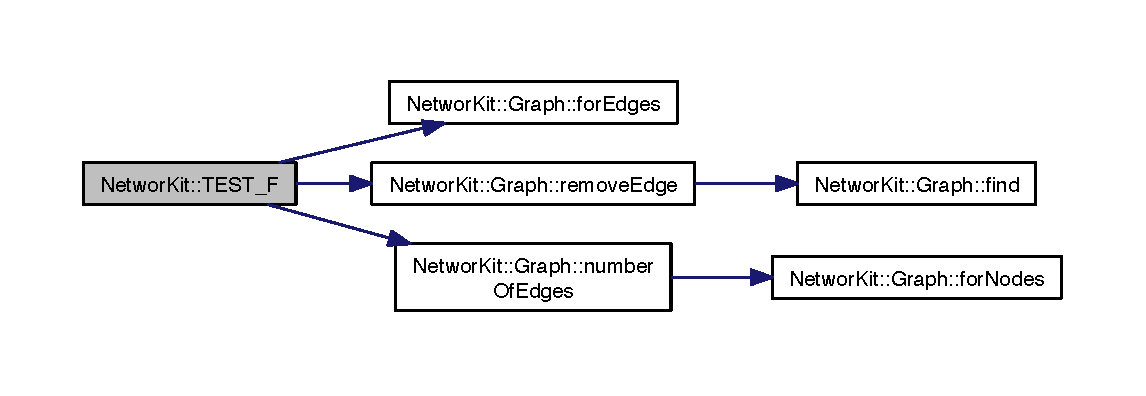
\includegraphics[width=350pt]{namespace_networ_kit_ae1c2725eb57fbfe2f0d42512d453d70a_cgraph}
\end{center}
\end{figure}


\hypertarget{namespace_networ_kit_a0ae784520b38efeaf8ae258e06db0fbf}{\index{Networ\-Kit@{Networ\-Kit}!T\-E\-S\-T\-\_\-\-F@{T\-E\-S\-T\-\_\-\-F}}
\index{T\-E\-S\-T\-\_\-\-F@{T\-E\-S\-T\-\_\-\-F}!NetworKit@{Networ\-Kit}}
\subsubsection[{T\-E\-S\-T\-\_\-\-F}]{\setlength{\rightskip}{0pt plus 5cm}Networ\-Kit\-::\-T\-E\-S\-T\-\_\-\-F (
\begin{DoxyParamCaption}
\item[{Coarsening\-G\-Test}]{, }
\item[{test\-Clustering\-Projector\-With\-Singleton\-Clustering}]{}
\end{DoxyParamCaption}
)}}\label{namespace_networ_kit_a0ae784520b38efeaf8ae258e06db0fbf}


Definition at line 66 of file Coarsening\-G\-Test.\-cpp.



Here is the call graph for this function\-:\nopagebreak
\begin{figure}[H]
\begin{center}
\leavevmode
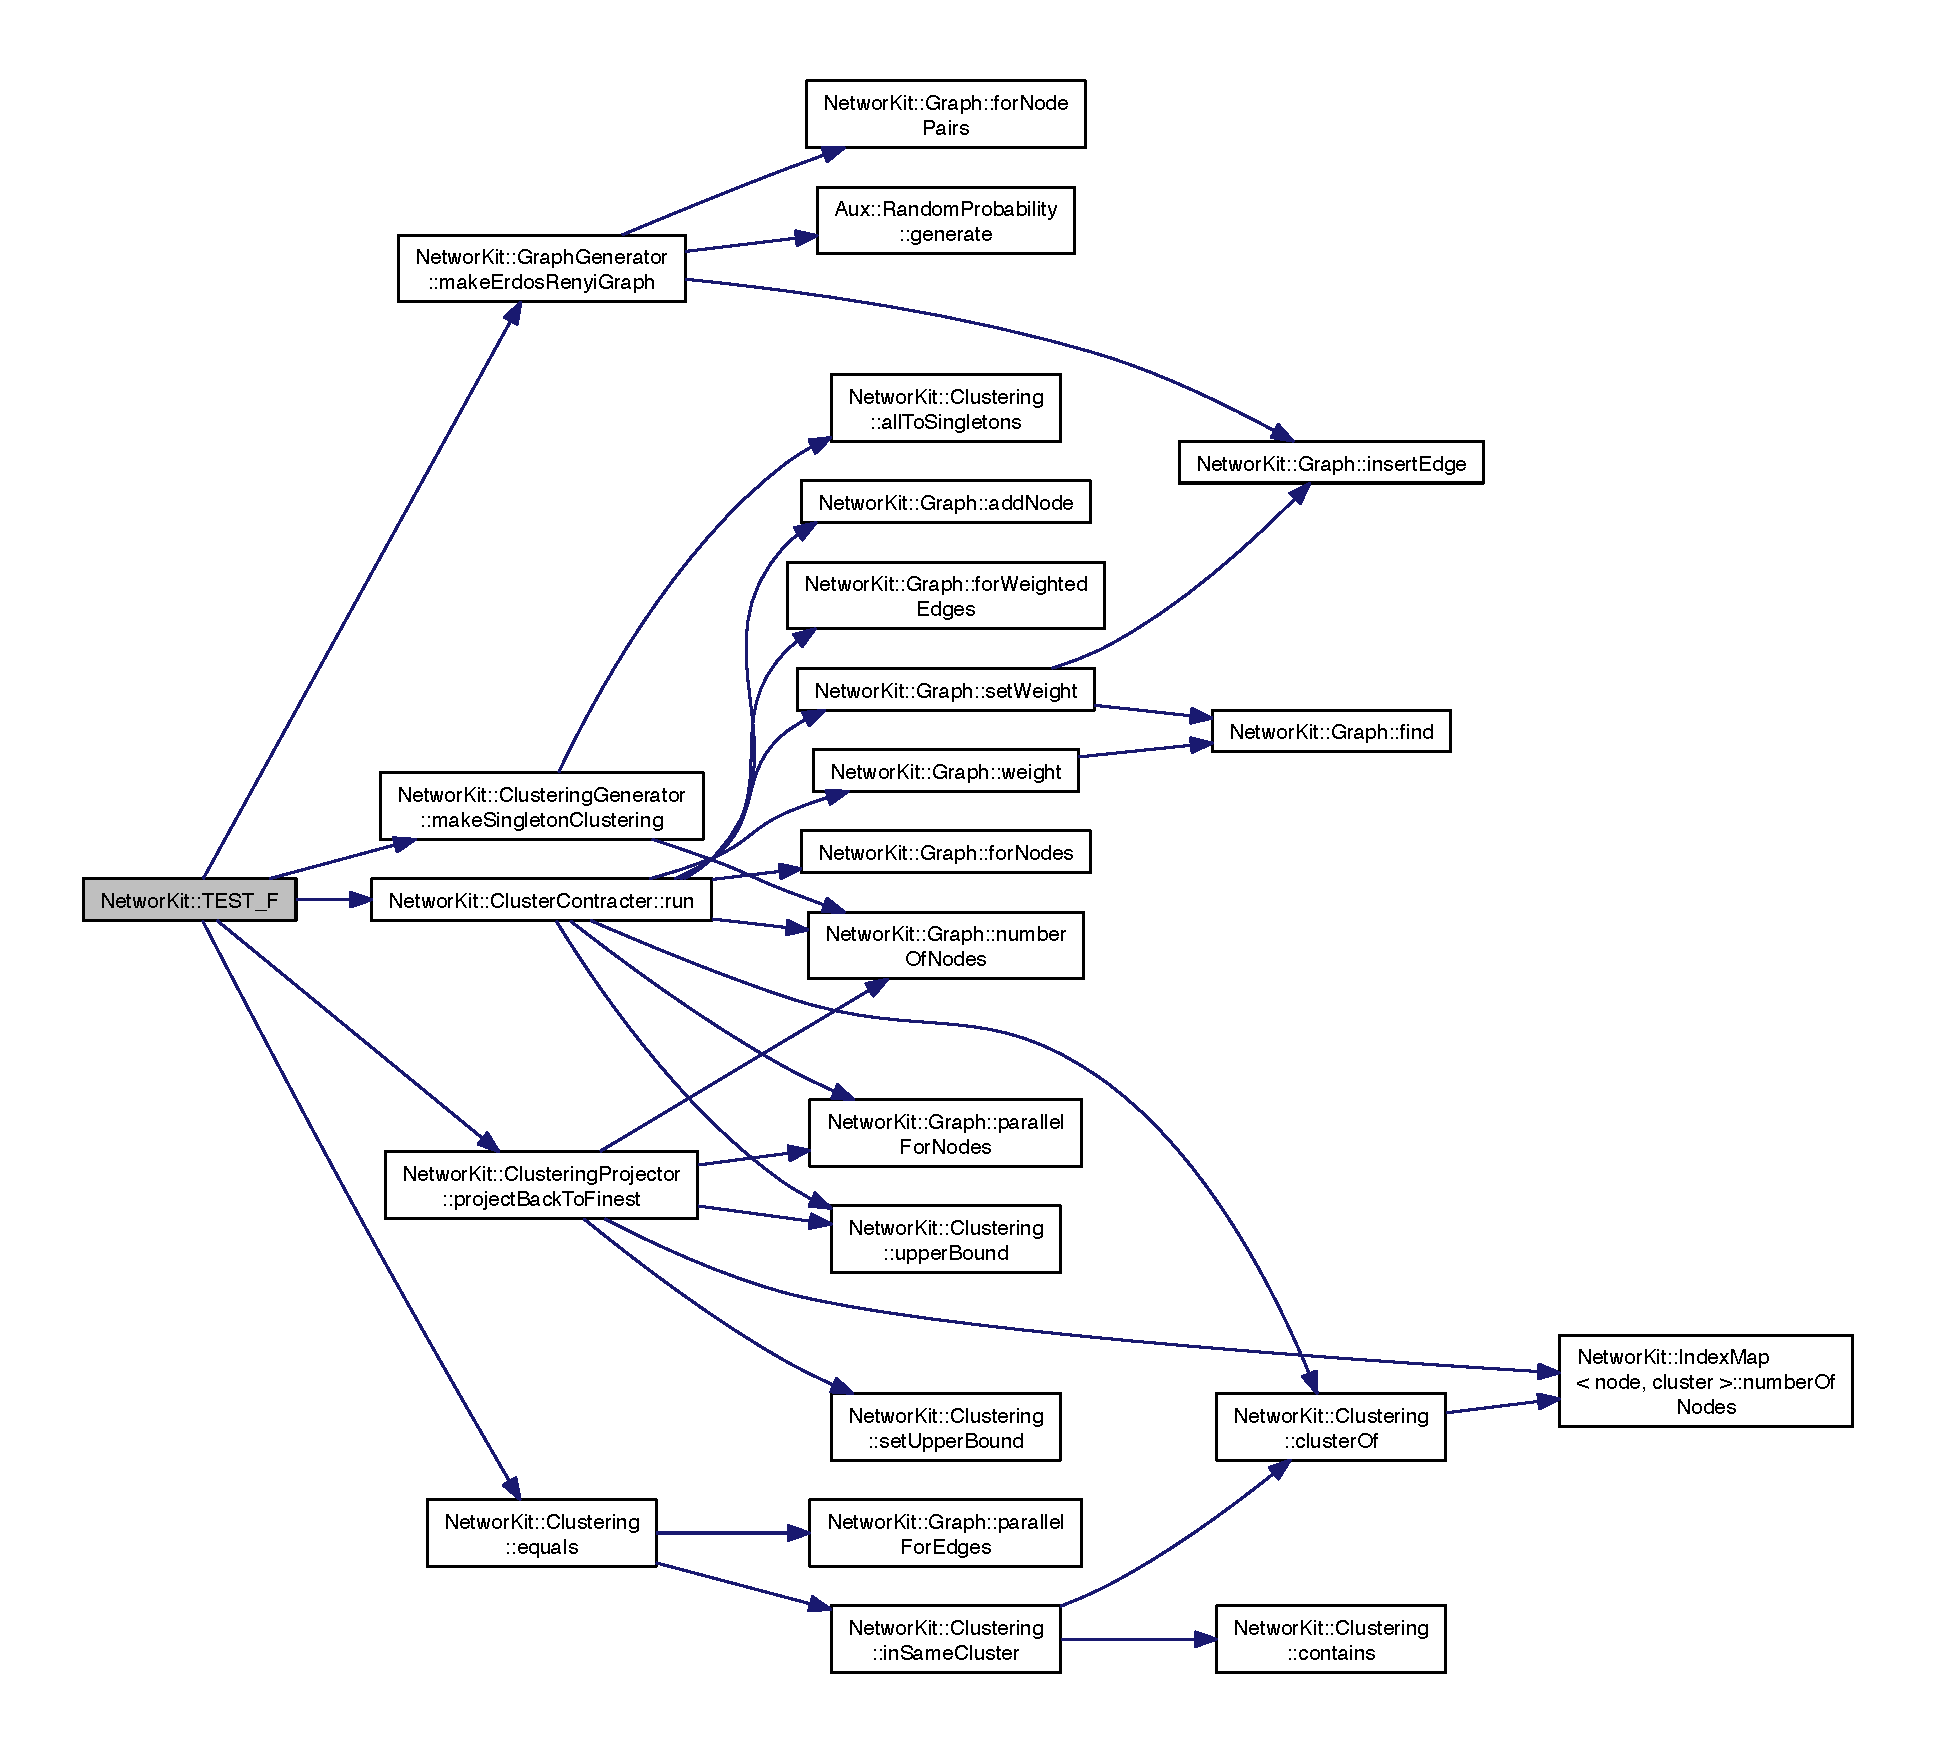
\includegraphics[width=350pt]{namespace_networ_kit_a0ae784520b38efeaf8ae258e06db0fbf_cgraph}
\end{center}
\end{figure}


\hypertarget{namespace_networ_kit_a95bf11f85605236d2f128edede2cfbd2}{\index{Networ\-Kit@{Networ\-Kit}!T\-E\-S\-T\-\_\-\-F@{T\-E\-S\-T\-\_\-\-F}}
\index{T\-E\-S\-T\-\_\-\-F@{T\-E\-S\-T\-\_\-\-F}!NetworKit@{Networ\-Kit}}
\subsubsection[{T\-E\-S\-T\-\_\-\-F}]{\setlength{\rightskip}{0pt plus 5cm}Networ\-Kit\-::\-T\-E\-S\-T\-\_\-\-F (
\begin{DoxyParamCaption}
\item[{Basics\-Benchmark}]{, }
\item[{parallel\-Sum\-Reduction}]{}
\end{DoxyParamCaption}
)}}\label{namespace_networ_kit_a95bf11f85605236d2f128edede2cfbd2}


Definition at line 70 of file Basics\-Benchmark.\-cpp.



Here is the call graph for this function\-:\nopagebreak
\begin{figure}[H]
\begin{center}
\leavevmode
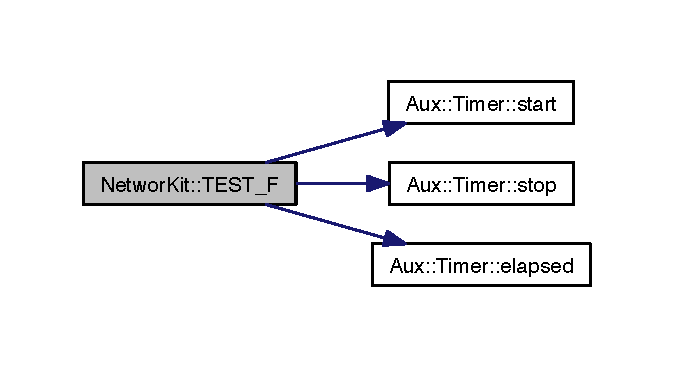
\includegraphics[width=324pt]{namespace_networ_kit_a95bf11f85605236d2f128edede2cfbd2_cgraph}
\end{center}
\end{figure}


\hypertarget{namespace_networ_kit_a39a05014d6ee7cef8919323aef8900b5}{\index{Networ\-Kit@{Networ\-Kit}!T\-E\-S\-T\-\_\-\-F@{T\-E\-S\-T\-\_\-\-F}}
\index{T\-E\-S\-T\-\_\-\-F@{T\-E\-S\-T\-\_\-\-F}!NetworKit@{Networ\-Kit}}
\subsubsection[{T\-E\-S\-T\-\_\-\-F}]{\setlength{\rightskip}{0pt plus 5cm}Networ\-Kit\-::\-T\-E\-S\-T\-\_\-\-F (
\begin{DoxyParamCaption}
\item[{Overlap\-G\-Test}]{, }
\item[{test\-Hashing}]{}
\end{DoxyParamCaption}
)}}\label{namespace_networ_kit_a39a05014d6ee7cef8919323aef8900b5}


Definition at line 71 of file Overlap\-G\-Test.\-cpp.

\hypertarget{namespace_networ_kit_a9123d4b22507a6441651434fb666892d}{\index{Networ\-Kit@{Networ\-Kit}!T\-E\-S\-T\-\_\-\-F@{T\-E\-S\-T\-\_\-\-F}}
\index{T\-E\-S\-T\-\_\-\-F@{T\-E\-S\-T\-\_\-\-F}!NetworKit@{Networ\-Kit}}
\subsubsection[{T\-E\-S\-T\-\_\-\-F}]{\setlength{\rightskip}{0pt plus 5cm}Networ\-Kit\-::\-T\-E\-S\-T\-\_\-\-F (
\begin{DoxyParamCaption}
\item[{Input\-G\-Test}]{, }
\item[{test\-Clustering\-Writer\-And\-Reader}]{}
\end{DoxyParamCaption}
)}}\label{namespace_networ_kit_a9123d4b22507a6441651434fb666892d}


Definition at line 72 of file Input\-G\-Test.\-cpp.



Here is the call graph for this function\-:\nopagebreak
\begin{figure}[H]
\begin{center}
\leavevmode
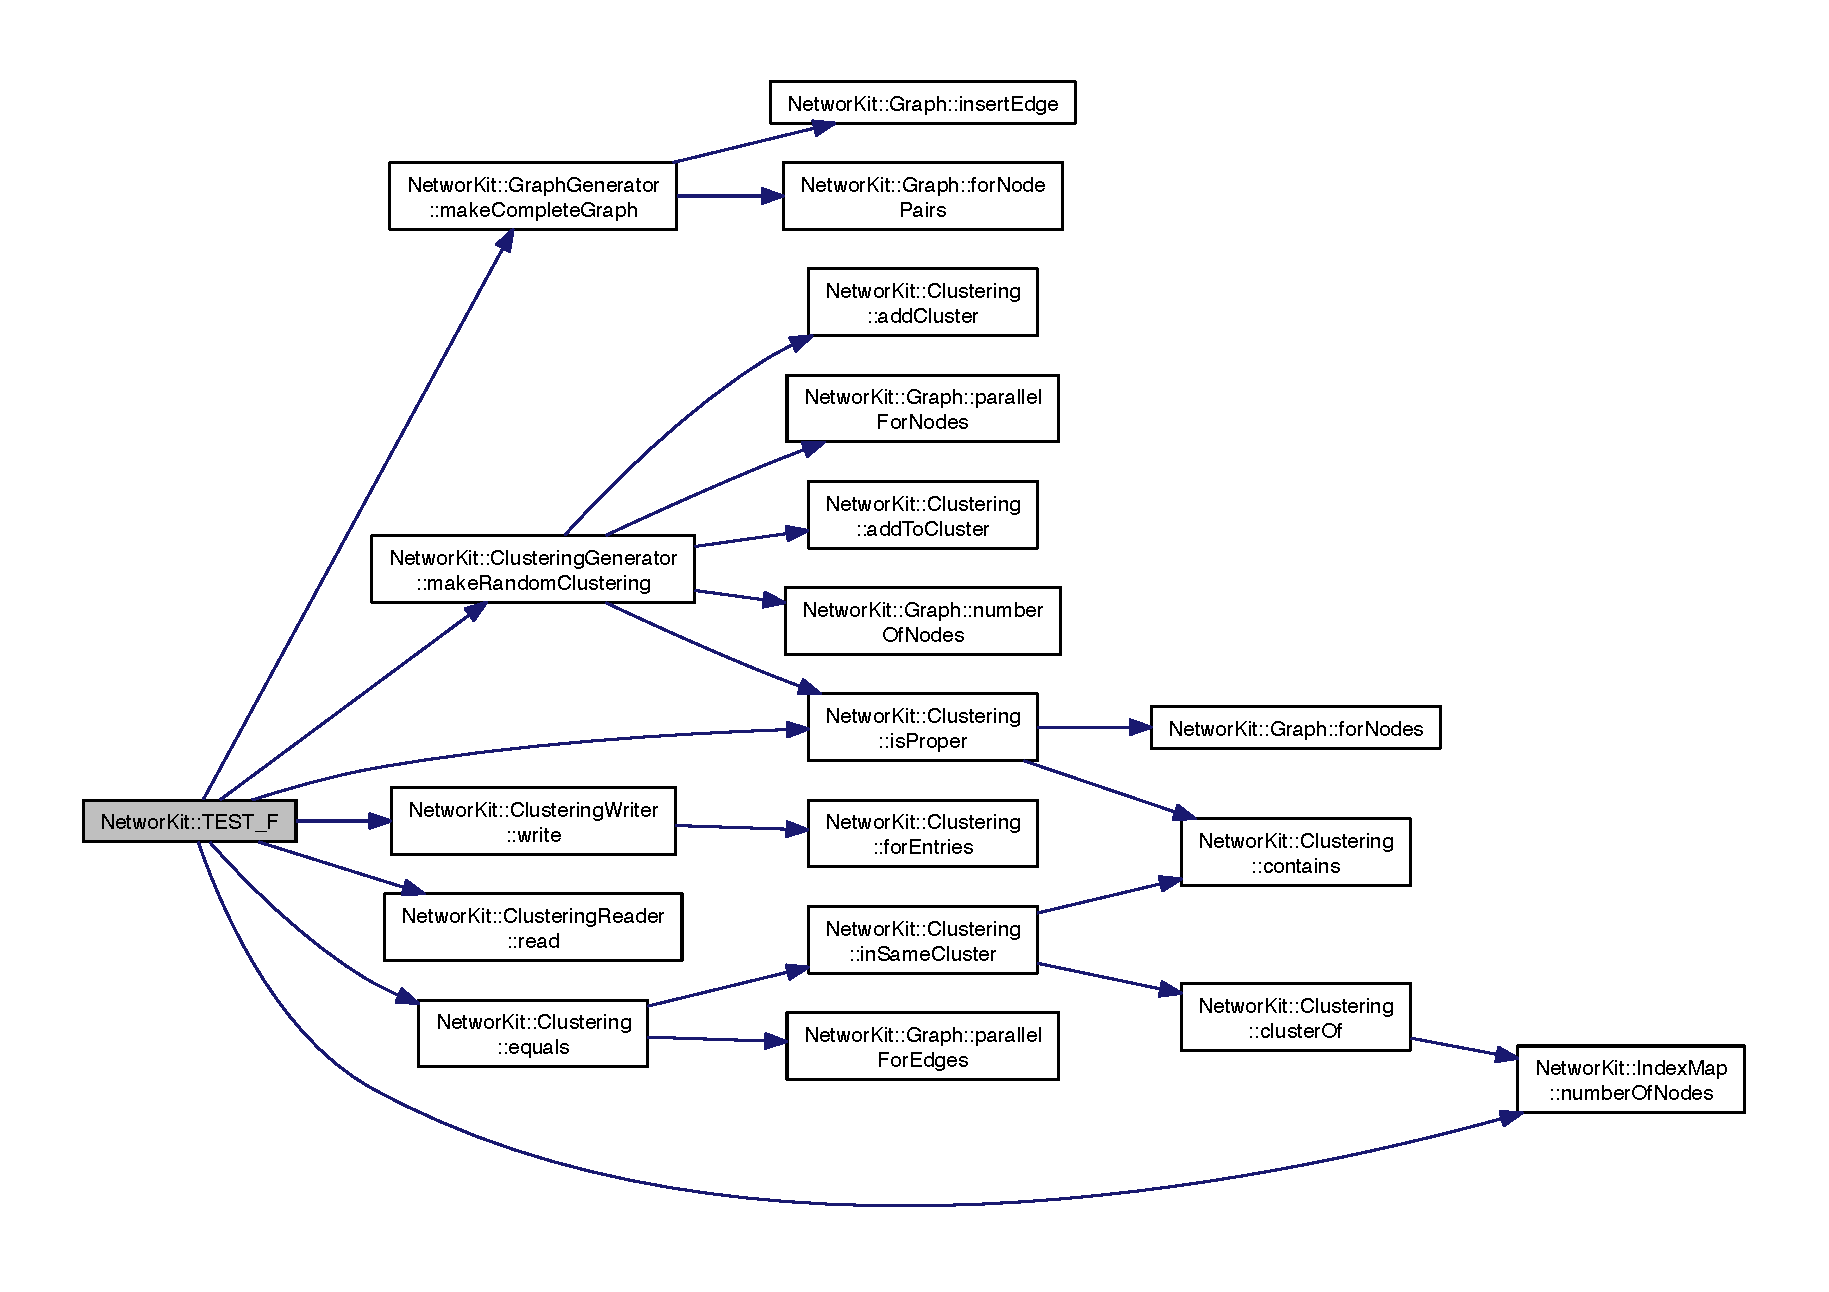
\includegraphics[width=350pt]{namespace_networ_kit_a9123d4b22507a6441651434fb666892d_cgraph}
\end{center}
\end{figure}


\hypertarget{namespace_networ_kit_addea5bddd0f76b73a69418ab374aeb40}{\index{Networ\-Kit@{Networ\-Kit}!T\-E\-S\-T\-\_\-\-F@{T\-E\-S\-T\-\_\-\-F}}
\index{T\-E\-S\-T\-\_\-\-F@{T\-E\-S\-T\-\_\-\-F}!NetworKit@{Networ\-Kit}}
\subsubsection[{T\-E\-S\-T\-\_\-\-F}]{\setlength{\rightskip}{0pt plus 5cm}Networ\-Kit\-::\-T\-E\-S\-T\-\_\-\-F (
\begin{DoxyParamCaption}
\item[{Graph2\-Benchmark}]{, }
\item[{node\-Pair\-Iteration}]{}
\end{DoxyParamCaption}
)}}\label{namespace_networ_kit_addea5bddd0f76b73a69418ab374aeb40}


Definition at line 75 of file Graph2\-Benchmark.\-cpp.



Here is the call graph for this function\-:\nopagebreak
\begin{figure}[H]
\begin{center}
\leavevmode
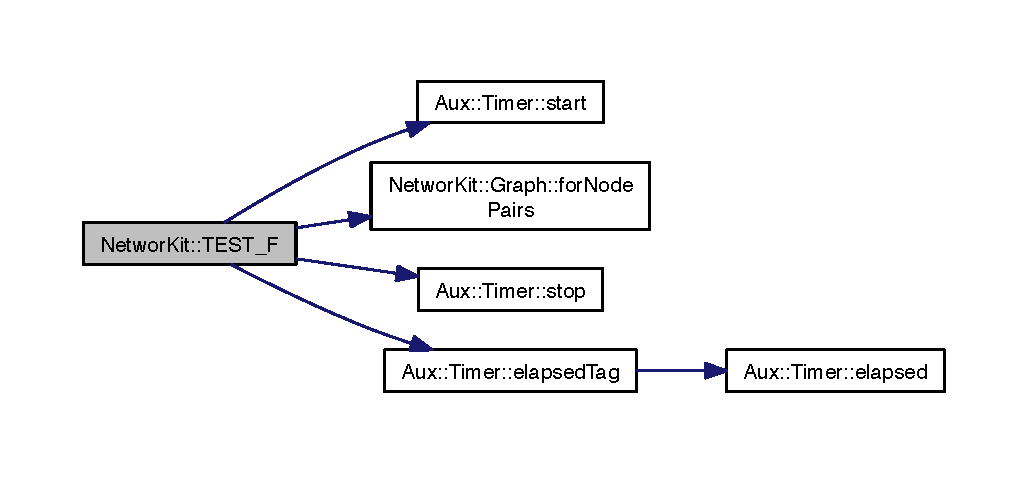
\includegraphics[width=350pt]{namespace_networ_kit_addea5bddd0f76b73a69418ab374aeb40_cgraph}
\end{center}
\end{figure}


\hypertarget{namespace_networ_kit_a2a306d74607ec520cad796ad6603f093}{\index{Networ\-Kit@{Networ\-Kit}!T\-E\-S\-T\-\_\-\-F@{T\-E\-S\-T\-\_\-\-F}}
\index{T\-E\-S\-T\-\_\-\-F@{T\-E\-S\-T\-\_\-\-F}!NetworKit@{Networ\-Kit}}
\subsubsection[{T\-E\-S\-T\-\_\-\-F}]{\setlength{\rightskip}{0pt plus 5cm}Networ\-Kit\-::\-T\-E\-S\-T\-\_\-\-F (
\begin{DoxyParamCaption}
\item[{Clustering\-Algo\-G\-Test}]{, }
\item[{test\-Label\-Propagation\-On\-Disconnected\-Graph}]{}
\end{DoxyParamCaption}
)}}\label{namespace_networ_kit_a2a306d74607ec520cad796ad6603f093}


Definition at line 77 of file Clustering\-Algo\-G\-Test.\-cpp.



Here is the call graph for this function\-:\nopagebreak
\begin{figure}[H]
\begin{center}
\leavevmode
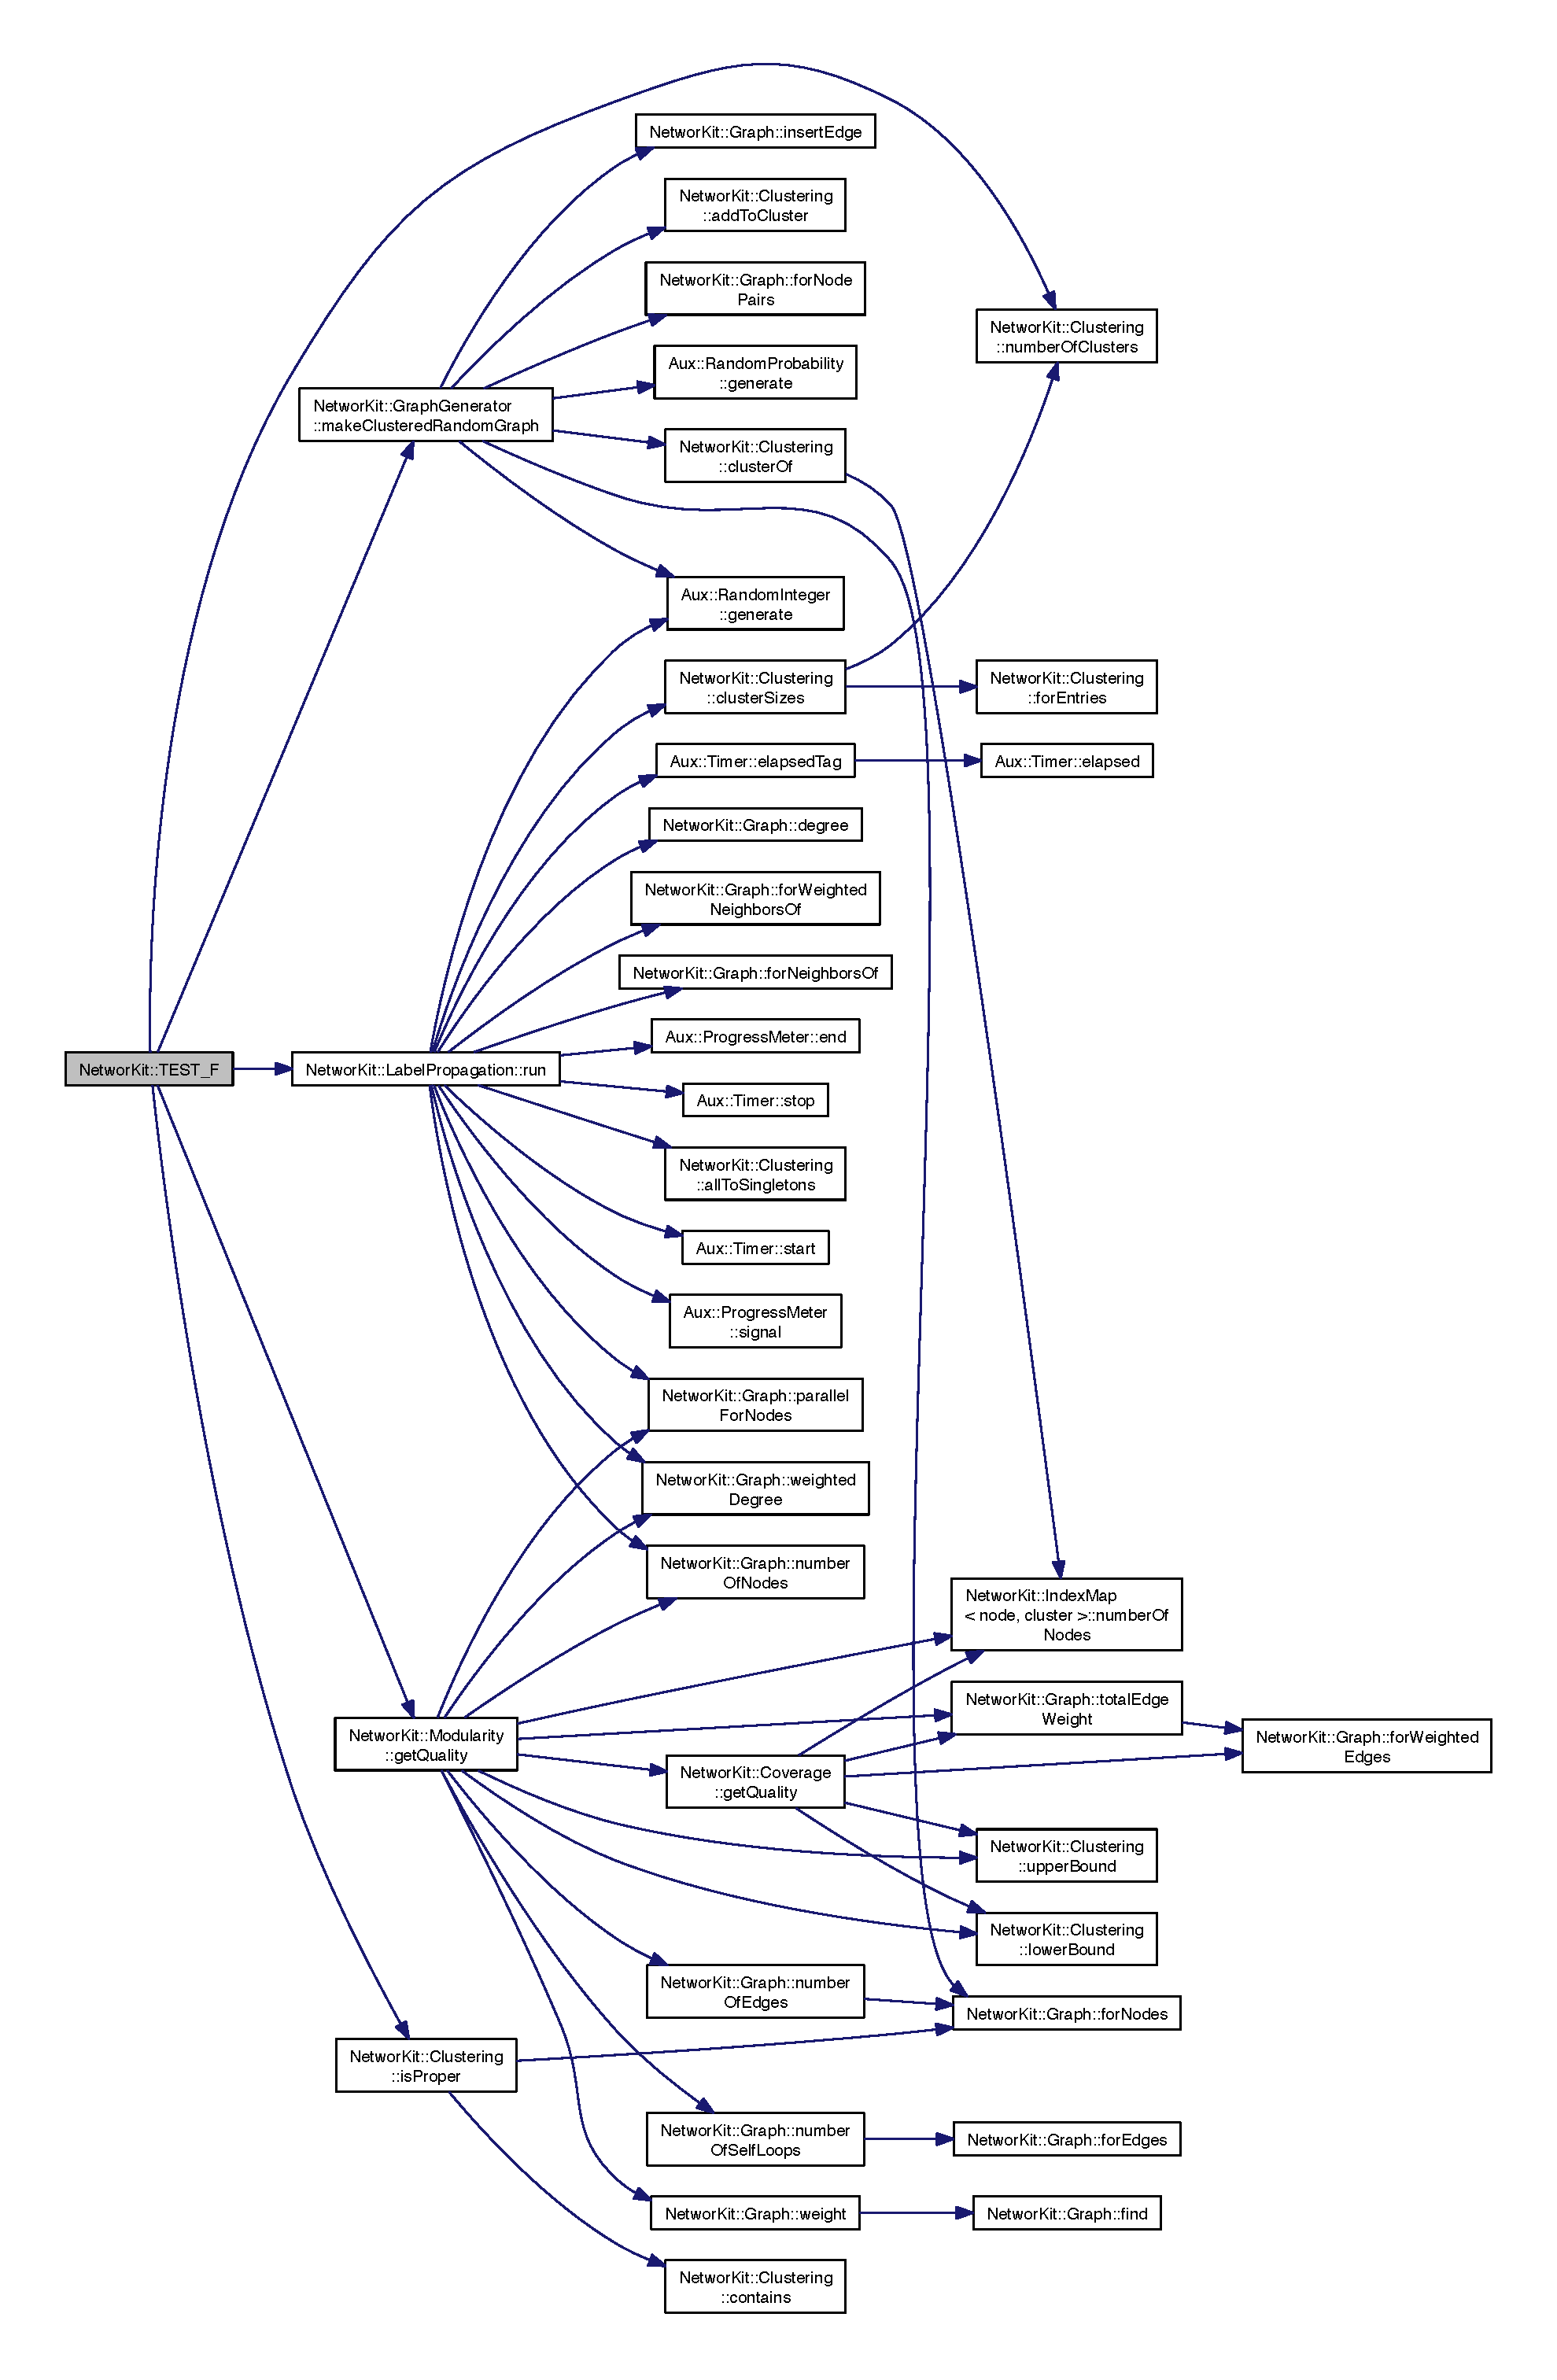
\includegraphics[width=350pt]{namespace_networ_kit_a2a306d74607ec520cad796ad6603f093_cgraph}
\end{center}
\end{figure}


\hypertarget{namespace_networ_kit_aa5ae2d52c221f413c51b5432eb36a88f}{\index{Networ\-Kit@{Networ\-Kit}!T\-E\-S\-T\-\_\-\-F@{T\-E\-S\-T\-\_\-\-F}}
\index{T\-E\-S\-T\-\_\-\-F@{T\-E\-S\-T\-\_\-\-F}!NetworKit@{Networ\-Kit}}
\subsubsection[{T\-E\-S\-T\-\_\-\-F}]{\setlength{\rightskip}{0pt plus 5cm}Networ\-Kit\-::\-T\-E\-S\-T\-\_\-\-F (
\begin{DoxyParamCaption}
\item[{Graph\-G\-Test}]{, }
\item[{test\-Lambda\-Node\-Iteration}]{}
\end{DoxyParamCaption}
)}}\label{namespace_networ_kit_aa5ae2d52c221f413c51b5432eb36a88f}


Definition at line 80 of file Graph\-G\-Test.\-cpp.



Here is the call graph for this function\-:\nopagebreak
\begin{figure}[H]
\begin{center}
\leavevmode
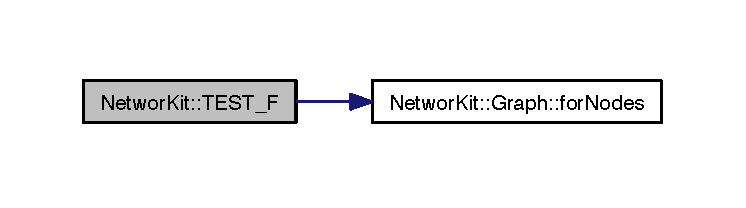
\includegraphics[width=350pt]{namespace_networ_kit_aa5ae2d52c221f413c51b5432eb36a88f_cgraph}
\end{center}
\end{figure}


\hypertarget{namespace_networ_kit_afe44bdb419de446e1d0b18cc54dd356a}{\index{Networ\-Kit@{Networ\-Kit}!T\-E\-S\-T\-\_\-\-F@{T\-E\-S\-T\-\_\-\-F}}
\index{T\-E\-S\-T\-\_\-\-F@{T\-E\-S\-T\-\_\-\-F}!NetworKit@{Networ\-Kit}}
\subsubsection[{T\-E\-S\-T\-\_\-\-F}]{\setlength{\rightskip}{0pt plus 5cm}Networ\-Kit\-::\-T\-E\-S\-T\-\_\-\-F (
\begin{DoxyParamCaption}
\item[{Clustering\-G\-Test}]{, }
\item[{test\-Clustering\-Equality}]{}
\end{DoxyParamCaption}
)}}\label{namespace_networ_kit_afe44bdb419de446e1d0b18cc54dd356a}


Definition at line 80 of file Clustering\-G\-Test.\-cpp.



Here is the call graph for this function\-:\nopagebreak
\begin{figure}[H]
\begin{center}
\leavevmode
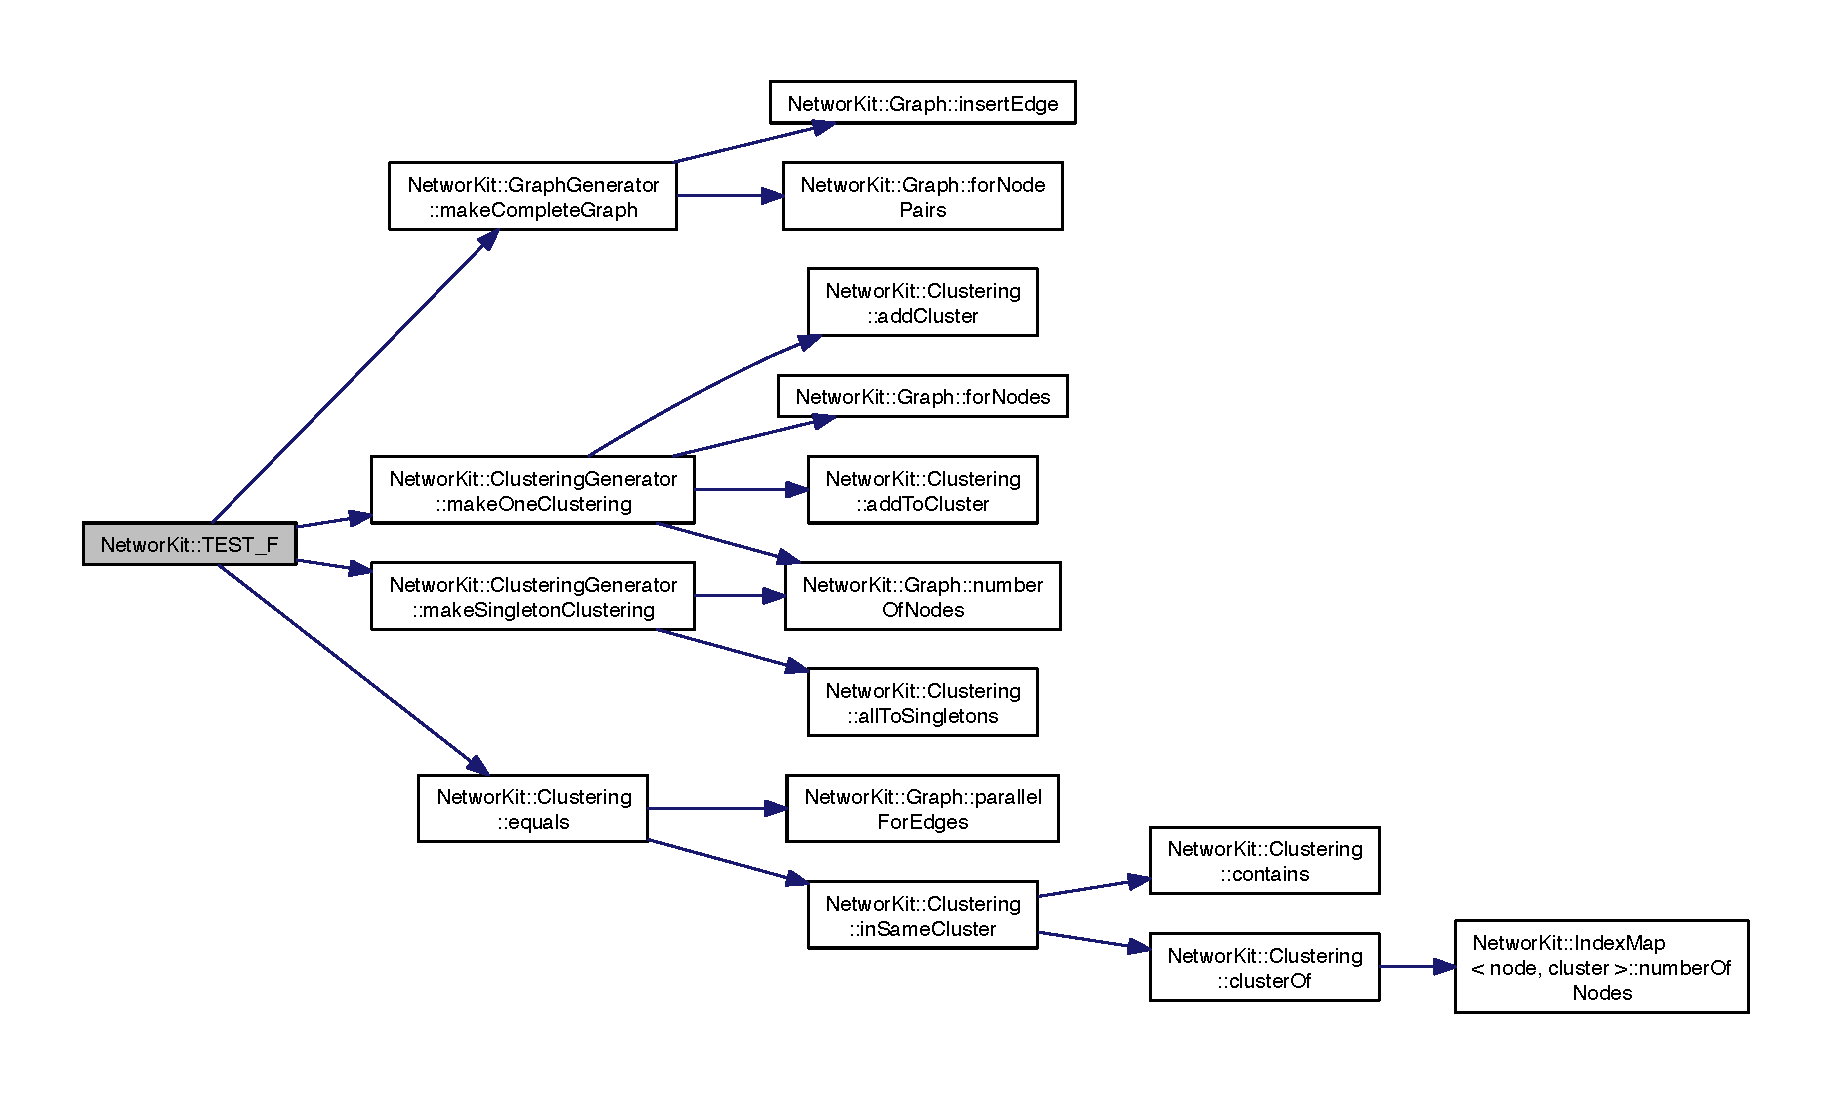
\includegraphics[width=350pt]{namespace_networ_kit_afe44bdb419de446e1d0b18cc54dd356a_cgraph}
\end{center}
\end{figure}


\hypertarget{namespace_networ_kit_a1eda995441aa07c4b81db34b4f534bfe}{\index{Networ\-Kit@{Networ\-Kit}!T\-E\-S\-T\-\_\-\-F@{T\-E\-S\-T\-\_\-\-F}}
\index{T\-E\-S\-T\-\_\-\-F@{T\-E\-S\-T\-\_\-\-F}!NetworKit@{Networ\-Kit}}
\subsubsection[{T\-E\-S\-T\-\_\-\-F}]{\setlength{\rightskip}{0pt plus 5cm}Networ\-Kit\-::\-T\-E\-S\-T\-\_\-\-F (
\begin{DoxyParamCaption}
\item[{Overlap\-G\-Test}]{, }
\item[{test\-Hashing\-Overlapper\-On\-Singleton\-Clusterings}]{}
\end{DoxyParamCaption}
)}}\label{namespace_networ_kit_a1eda995441aa07c4b81db34b4f534bfe}


Definition at line 85 of file Overlap\-G\-Test.\-cpp.



Here is the call graph for this function\-:\nopagebreak
\begin{figure}[H]
\begin{center}
\leavevmode
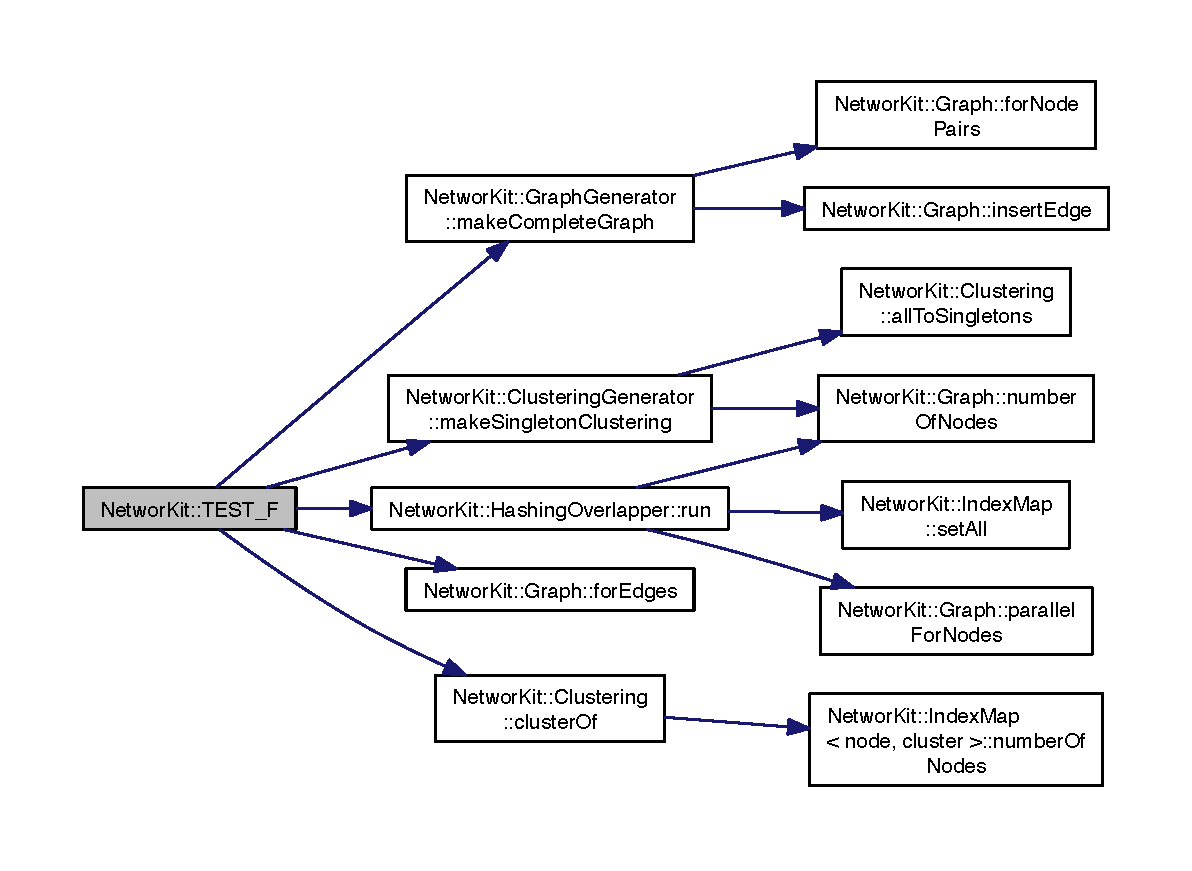
\includegraphics[width=350pt]{namespace_networ_kit_a1eda995441aa07c4b81db34b4f534bfe_cgraph}
\end{center}
\end{figure}


\hypertarget{namespace_networ_kit_a458b18e5bd29a405883b670653c58adf}{\index{Networ\-Kit@{Networ\-Kit}!T\-E\-S\-T\-\_\-\-F@{T\-E\-S\-T\-\_\-\-F}}
\index{T\-E\-S\-T\-\_\-\-F@{T\-E\-S\-T\-\_\-\-F}!NetworKit@{Networ\-Kit}}
\subsubsection[{T\-E\-S\-T\-\_\-\-F}]{\setlength{\rightskip}{0pt plus 5cm}Networ\-Kit\-::\-T\-E\-S\-T\-\_\-\-F (
\begin{DoxyParamCaption}
\item[{Graph2\-G\-Test}]{, }
\item[{test\-Node\-Iteration}]{}
\end{DoxyParamCaption}
)}}\label{namespace_networ_kit_a458b18e5bd29a405883b670653c58adf}


Definition at line 91 of file Graph2\-G\-Test.\-cpp.



Here is the call graph for this function\-:\nopagebreak
\begin{figure}[H]
\begin{center}
\leavevmode
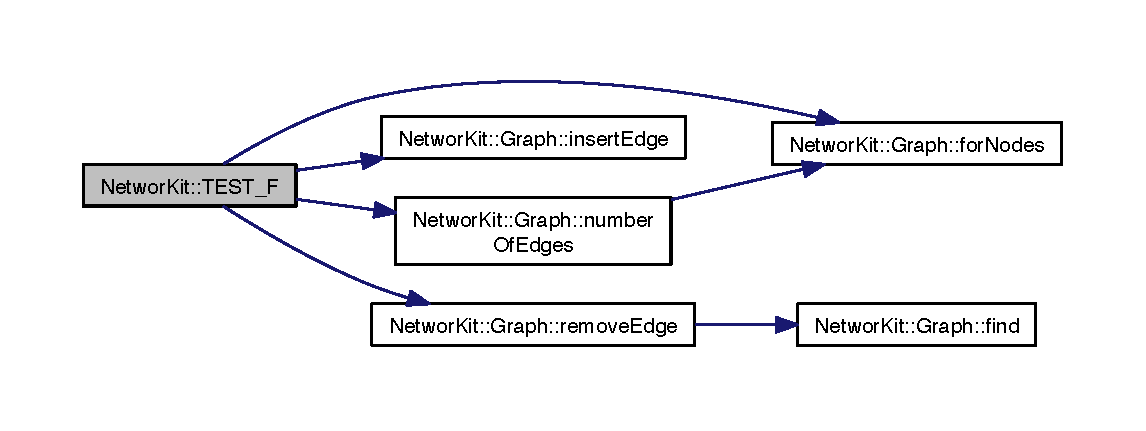
\includegraphics[width=350pt]{namespace_networ_kit_a458b18e5bd29a405883b670653c58adf_cgraph}
\end{center}
\end{figure}


\hypertarget{namespace_networ_kit_a1eced118aec8d8c268f8db89355e9b41}{\index{Networ\-Kit@{Networ\-Kit}!T\-E\-S\-T\-\_\-\-F@{T\-E\-S\-T\-\_\-\-F}}
\index{T\-E\-S\-T\-\_\-\-F@{T\-E\-S\-T\-\_\-\-F}!NetworKit@{Networ\-Kit}}
\subsubsection[{T\-E\-S\-T\-\_\-\-F}]{\setlength{\rightskip}{0pt plus 5cm}Networ\-Kit\-::\-T\-E\-S\-T\-\_\-\-F (
\begin{DoxyParamCaption}
\item[{Graph\-G\-Test}]{, }
\item[{test\-Parallel\-Lambda\-Node\-Iteration}]{}
\end{DoxyParamCaption}
)}}\label{namespace_networ_kit_a1eced118aec8d8c268f8db89355e9b41}


Definition at line 94 of file Graph\-G\-Test.\-cpp.



Here is the call graph for this function\-:\nopagebreak
\begin{figure}[H]
\begin{center}
\leavevmode
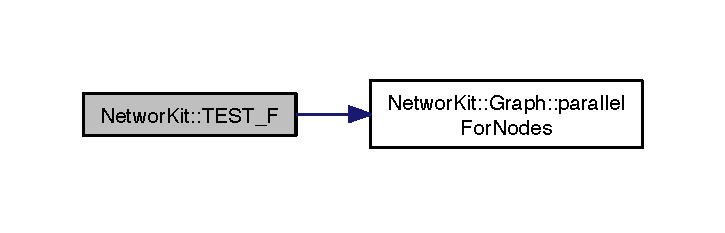
\includegraphics[width=348pt]{namespace_networ_kit_a1eced118aec8d8c268f8db89355e9b41_cgraph}
\end{center}
\end{figure}


\hypertarget{namespace_networ_kit_ab4a7126555e635ad80bb0f05a587b237}{\index{Networ\-Kit@{Networ\-Kit}!T\-E\-S\-T\-\_\-\-F@{T\-E\-S\-T\-\_\-\-F}}
\index{T\-E\-S\-T\-\_\-\-F@{T\-E\-S\-T\-\_\-\-F}!NetworKit@{Networ\-Kit}}
\subsubsection[{T\-E\-S\-T\-\_\-\-F}]{\setlength{\rightskip}{0pt plus 5cm}Networ\-Kit\-::\-T\-E\-S\-T\-\_\-\-F (
\begin{DoxyParamCaption}
\item[{Clustering\-Algo\-G\-Test}]{, }
\item[{test\-Label\-Propagation\-On\-Single\-Node\-With\-Self\-Loop}]{}
\end{DoxyParamCaption}
)}}\label{namespace_networ_kit_ab4a7126555e635ad80bb0f05a587b237}


Definition at line 96 of file Clustering\-Algo\-G\-Test.\-cpp.



Here is the call graph for this function\-:\nopagebreak
\begin{figure}[H]
\begin{center}
\leavevmode
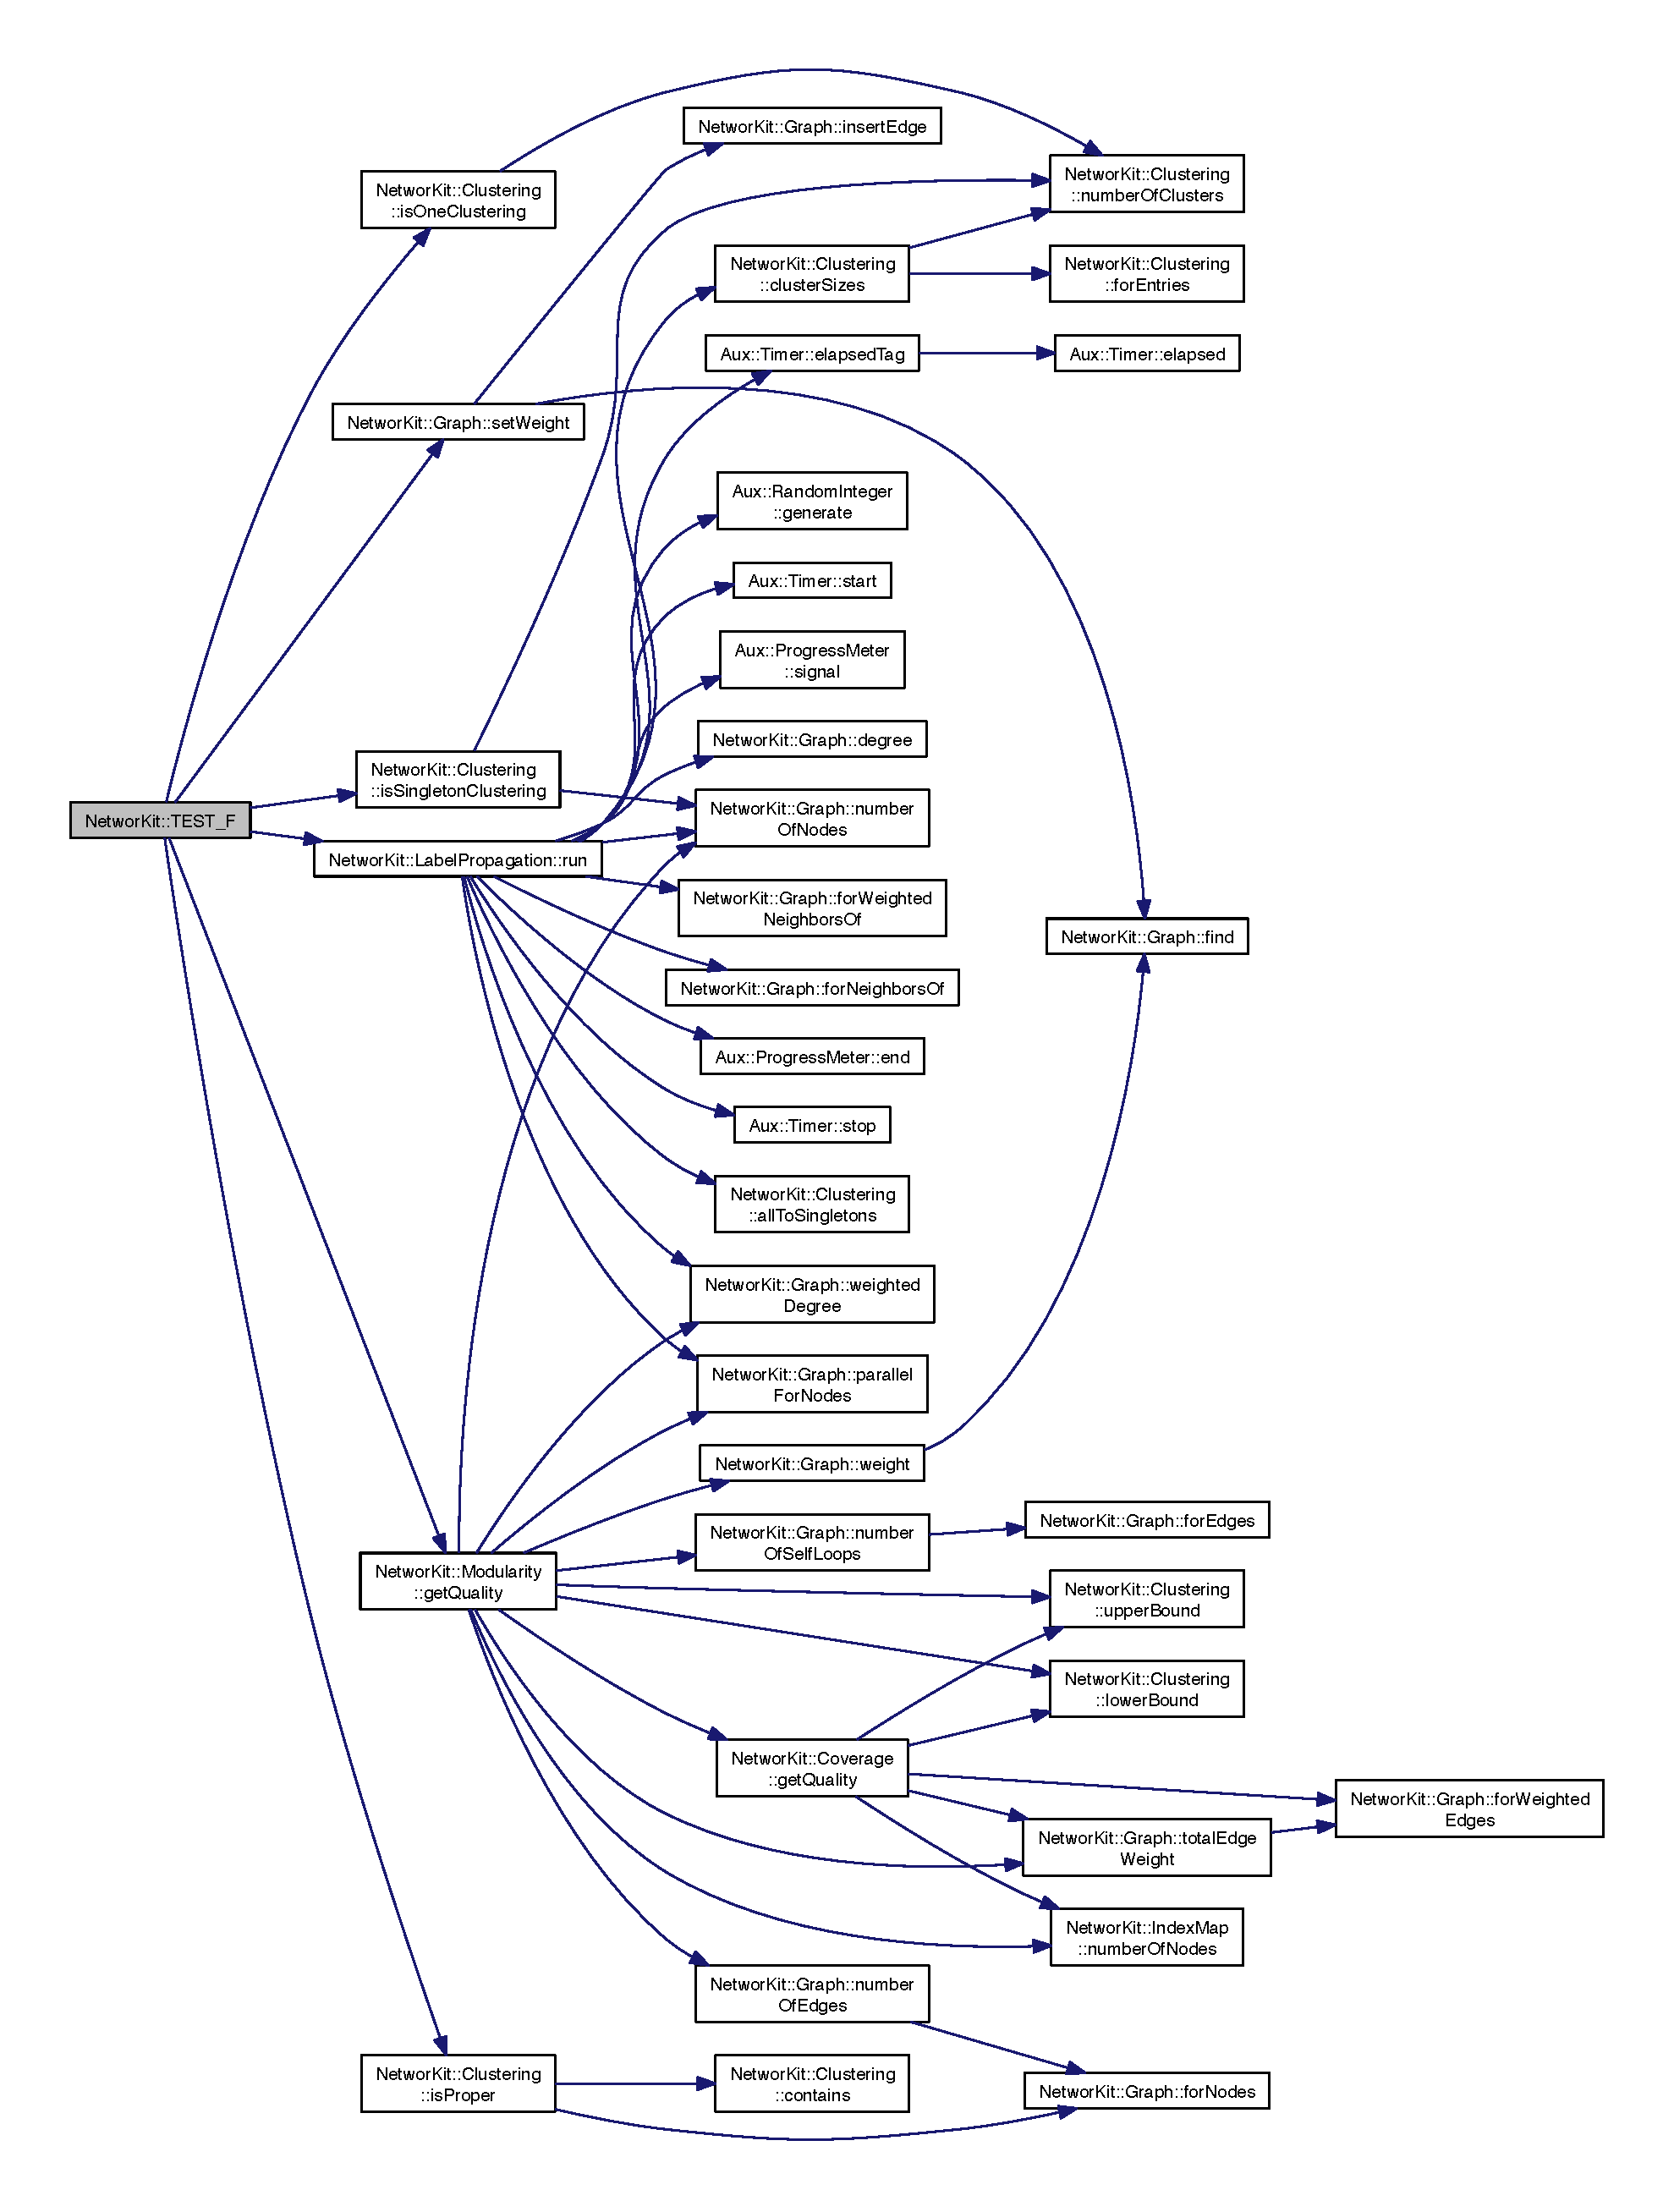
\includegraphics[width=350pt]{namespace_networ_kit_ab4a7126555e635ad80bb0f05a587b237_cgraph}
\end{center}
\end{figure}


\hypertarget{namespace_networ_kit_a4b123ae13e55b0533142a9d1c6b60caa}{\index{Networ\-Kit@{Networ\-Kit}!T\-E\-S\-T\-\_\-\-F@{T\-E\-S\-T\-\_\-\-F}}
\index{T\-E\-S\-T\-\_\-\-F@{T\-E\-S\-T\-\_\-\-F}!NetworKit@{Networ\-Kit}}
\subsubsection[{T\-E\-S\-T\-\_\-\-F}]{\setlength{\rightskip}{0pt plus 5cm}Networ\-Kit\-::\-T\-E\-S\-T\-\_\-\-F (
\begin{DoxyParamCaption}
\item[{Graph2\-Benchmark}]{, }
\item[{edge\-Insertion}]{}
\end{DoxyParamCaption}
)}}\label{namespace_networ_kit_a4b123ae13e55b0533142a9d1c6b60caa}


Definition at line 96 of file Graph2\-Benchmark.\-cpp.



Here is the call graph for this function\-:\nopagebreak
\begin{figure}[H]
\begin{center}
\leavevmode
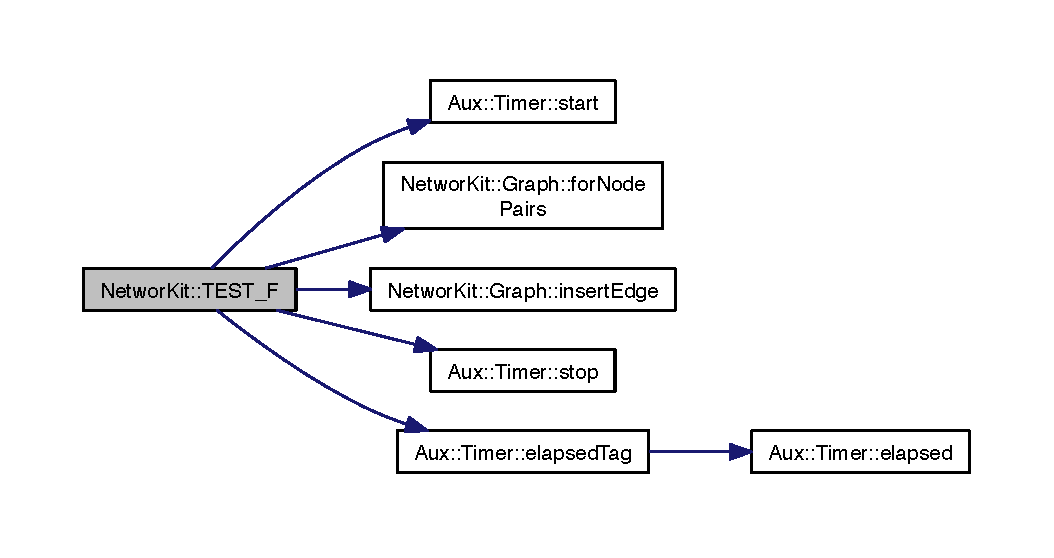
\includegraphics[width=350pt]{namespace_networ_kit_a4b123ae13e55b0533142a9d1c6b60caa_cgraph}
\end{center}
\end{figure}


\hypertarget{namespace_networ_kit_a0a7b4a1fa32e5f373fd606be55d76f54}{\index{Networ\-Kit@{Networ\-Kit}!T\-E\-S\-T\-\_\-\-F@{T\-E\-S\-T\-\_\-\-F}}
\index{T\-E\-S\-T\-\_\-\-F@{T\-E\-S\-T\-\_\-\-F}!NetworKit@{Networ\-Kit}}
\subsubsection[{T\-E\-S\-T\-\_\-\-F}]{\setlength{\rightskip}{0pt plus 5cm}Networ\-Kit\-::\-T\-E\-S\-T\-\_\-\-F (
\begin{DoxyParamCaption}
\item[{Clustering\-G\-Test}]{, }
\item[{test\-Jaccard\-Measure}]{}
\end{DoxyParamCaption}
)}}\label{namespace_networ_kit_a0a7b4a1fa32e5f373fd606be55d76f54}


Definition at line 100 of file Clustering\-G\-Test.\-cpp.



Here is the call graph for this function\-:\nopagebreak
\begin{figure}[H]
\begin{center}
\leavevmode
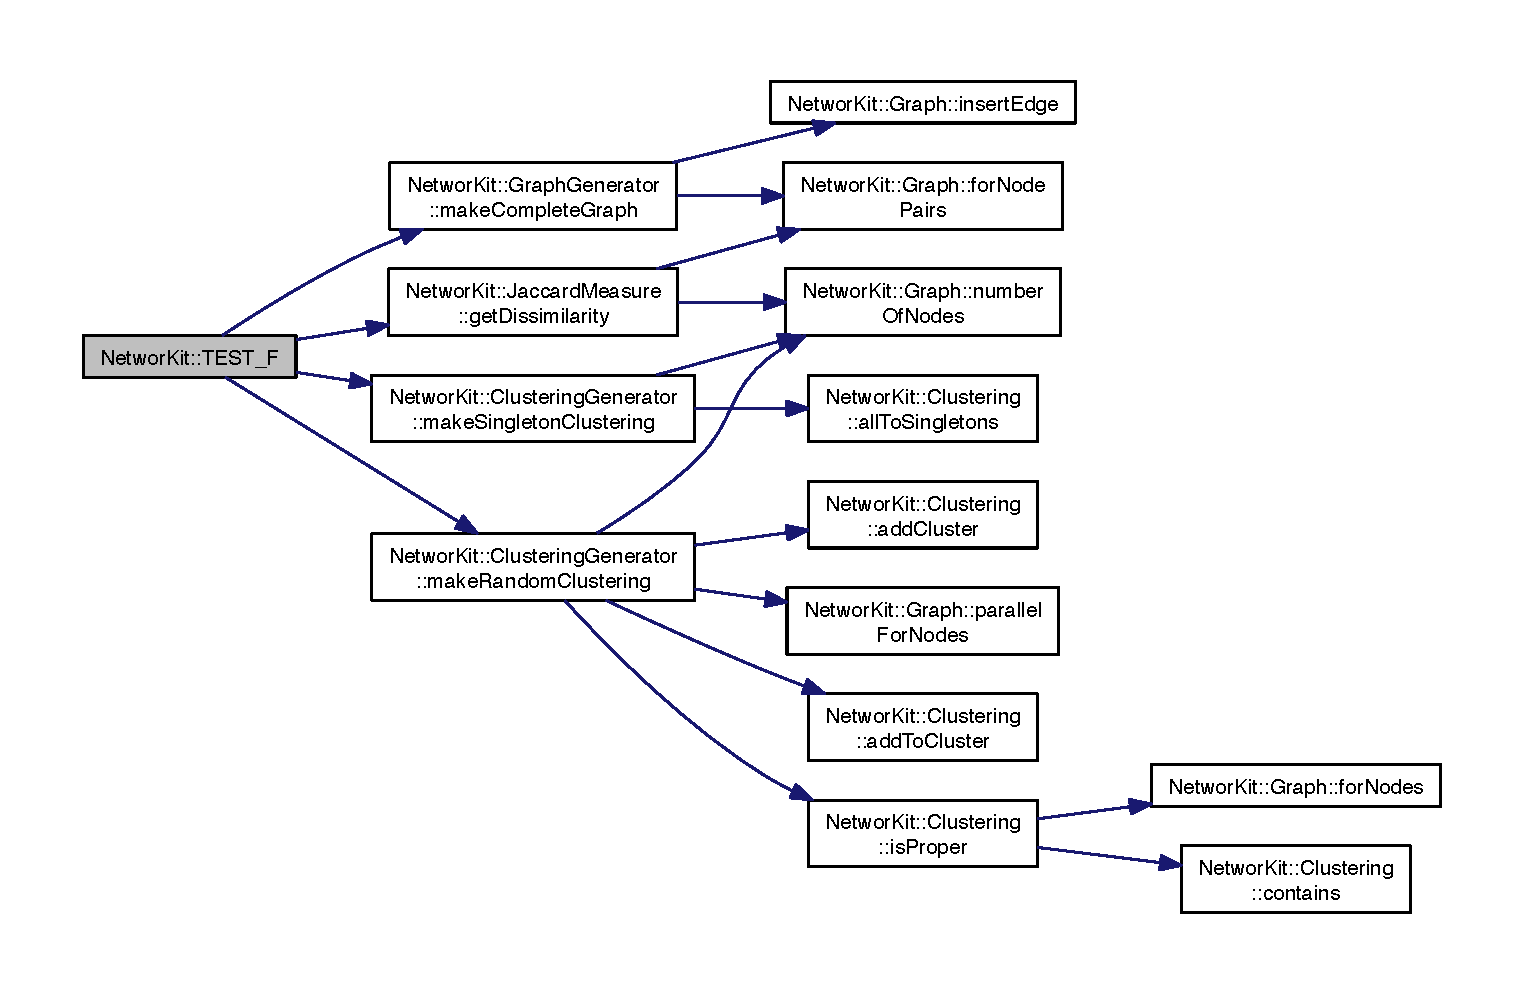
\includegraphics[width=350pt]{namespace_networ_kit_a0a7b4a1fa32e5f373fd606be55d76f54_cgraph}
\end{center}
\end{figure}


\hypertarget{namespace_networ_kit_a5b680dda57b4da22f8475528748fb4ca}{\index{Networ\-Kit@{Networ\-Kit}!T\-E\-S\-T\-\_\-\-F@{T\-E\-S\-T\-\_\-\-F}}
\index{T\-E\-S\-T\-\_\-\-F@{T\-E\-S\-T\-\_\-\-F}!NetworKit@{Networ\-Kit}}
\subsubsection[{T\-E\-S\-T\-\_\-\-F}]{\setlength{\rightskip}{0pt plus 5cm}Networ\-Kit\-::\-T\-E\-S\-T\-\_\-\-F (
\begin{DoxyParamCaption}
\item[{Basics\-Benchmark}]{, }
\item[{seq\-Vector\-Write}]{}
\end{DoxyParamCaption}
)}}\label{namespace_networ_kit_a5b680dda57b4da22f8475528748fb4ca}


Definition at line 105 of file Basics\-Benchmark.\-cpp.



Here is the call graph for this function\-:\nopagebreak
\begin{figure}[H]
\begin{center}
\leavevmode
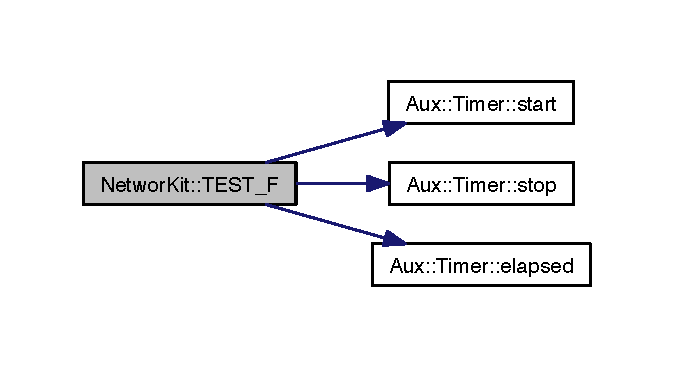
\includegraphics[width=324pt]{namespace_networ_kit_a5b680dda57b4da22f8475528748fb4ca_cgraph}
\end{center}
\end{figure}


\hypertarget{namespace_networ_kit_a2538cc231cd7f2daf364b5c1fb563c3f}{\index{Networ\-Kit@{Networ\-Kit}!T\-E\-S\-T\-\_\-\-F@{T\-E\-S\-T\-\_\-\-F}}
\index{T\-E\-S\-T\-\_\-\-F@{T\-E\-S\-T\-\_\-\-F}!NetworKit@{Networ\-Kit}}
\subsubsection[{T\-E\-S\-T\-\_\-\-F}]{\setlength{\rightskip}{0pt plus 5cm}Networ\-Kit\-::\-T\-E\-S\-T\-\_\-\-F (
\begin{DoxyParamCaption}
\item[{Graph\-G\-Test}]{, }
\item[{test\-Lambda\-Neighbor\-Iteration}]{}
\end{DoxyParamCaption}
)}}\label{namespace_networ_kit_a2538cc231cd7f2daf364b5c1fb563c3f}


Definition at line 109 of file Graph\-G\-Test.\-cpp.



Here is the call graph for this function\-:\nopagebreak
\begin{figure}[H]
\begin{center}
\leavevmode
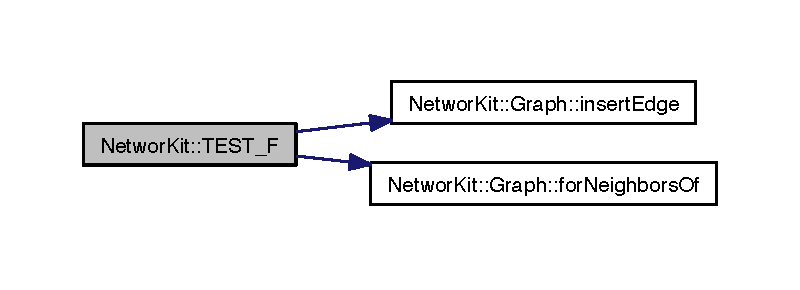
\includegraphics[width=350pt]{namespace_networ_kit_a2538cc231cd7f2daf364b5c1fb563c3f_cgraph}
\end{center}
\end{figure}


\hypertarget{namespace_networ_kit_ae7ef375b8f21824ce2907632ac29f148}{\index{Networ\-Kit@{Networ\-Kit}!T\-E\-S\-T\-\_\-\-F@{T\-E\-S\-T\-\_\-\-F}}
\index{T\-E\-S\-T\-\_\-\-F@{T\-E\-S\-T\-\_\-\-F}!NetworKit@{Networ\-Kit}}
\subsubsection[{T\-E\-S\-T\-\_\-\-F}]{\setlength{\rightskip}{0pt plus 5cm}Networ\-Kit\-::\-T\-E\-S\-T\-\_\-\-F (
\begin{DoxyParamCaption}
\item[{Graph2\-G\-Test}]{, }
\item[{test\-Parallel\-Edge\-Insertion}]{}
\end{DoxyParamCaption}
)}}\label{namespace_networ_kit_ae7ef375b8f21824ce2907632ac29f148}


Definition at line 109 of file Graph2\-G\-Test.\-cpp.



Here is the call graph for this function\-:\nopagebreak
\begin{figure}[H]
\begin{center}
\leavevmode
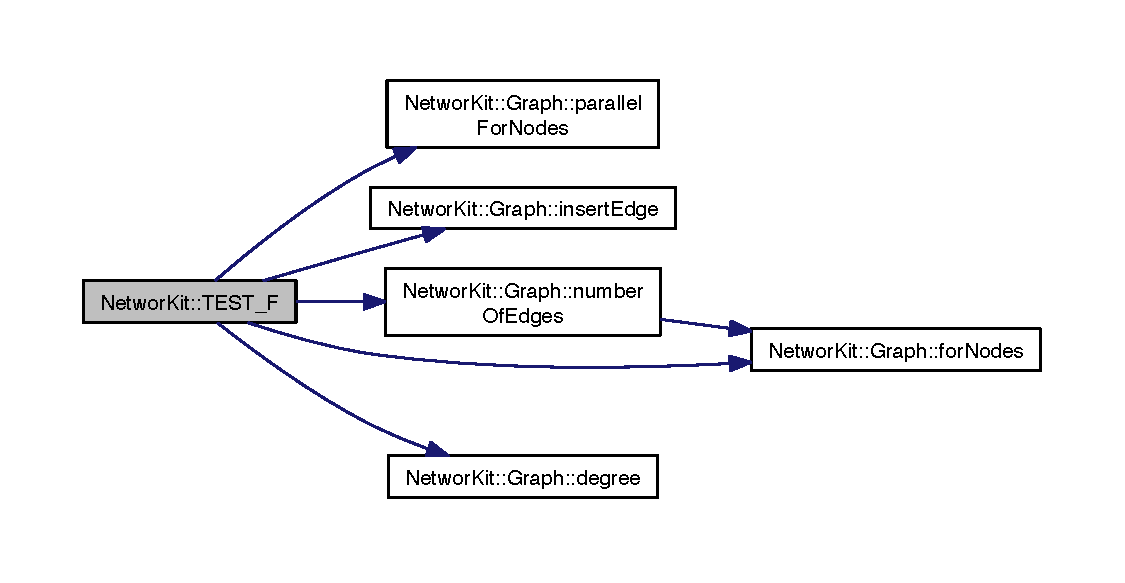
\includegraphics[width=350pt]{namespace_networ_kit_ae7ef375b8f21824ce2907632ac29f148_cgraph}
\end{center}
\end{figure}


\hypertarget{namespace_networ_kit_a3182533b4b9203b4d1acdddbe1b7f02c}{\index{Networ\-Kit@{Networ\-Kit}!T\-E\-S\-T\-\_\-\-F@{T\-E\-S\-T\-\_\-\-F}}
\index{T\-E\-S\-T\-\_\-\-F@{T\-E\-S\-T\-\_\-\-F}!NetworKit@{Networ\-Kit}}
\subsubsection[{T\-E\-S\-T\-\_\-\-F}]{\setlength{\rightskip}{0pt plus 5cm}Networ\-Kit\-::\-T\-E\-S\-T\-\_\-\-F (
\begin{DoxyParamCaption}
\item[{Overlap\-G\-Test}]{, }
\item[{test\-Hashing\-Overlapper\-On\-One\-Clusterings}]{}
\end{DoxyParamCaption}
)}}\label{namespace_networ_kit_a3182533b4b9203b4d1acdddbe1b7f02c}


Definition at line 110 of file Overlap\-G\-Test.\-cpp.



Here is the call graph for this function\-:\nopagebreak
\begin{figure}[H]
\begin{center}
\leavevmode
\includegraphics[width=350pt]{namespace_networ_kit_a3182533b4b9203b4d1acdddbe1b7f02c_cgraph}
\end{center}
\end{figure}


\hypertarget{namespace_networ_kit_afb6750a92496be71250132e4bd1a1fbf}{\index{Networ\-Kit@{Networ\-Kit}!T\-E\-S\-T\-\_\-\-F@{T\-E\-S\-T\-\_\-\-F}}
\index{T\-E\-S\-T\-\_\-\-F@{T\-E\-S\-T\-\_\-\-F}!NetworKit@{Networ\-Kit}}
\subsubsection[{T\-E\-S\-T\-\_\-\-F}]{\setlength{\rightskip}{0pt plus 5cm}Networ\-Kit\-::\-T\-E\-S\-T\-\_\-\-F (
\begin{DoxyParamCaption}
\item[{Ensemble\-G\-Test}]{, }
\item[{test\-Ensemble\-Clusterer\-On\-Almost\-Clique\-Graph}]{}
\end{DoxyParamCaption}
)}}\label{namespace_networ_kit_afb6750a92496be71250132e4bd1a1fbf}


Definition at line 114 of file Ensemble\-G\-Test.\-cpp.



Here is the call graph for this function\-:\nopagebreak
\begin{figure}[H]
\begin{center}
\leavevmode
\includegraphics[width=350pt]{namespace_networ_kit_afb6750a92496be71250132e4bd1a1fbf_cgraph}
\end{center}
\end{figure}


\hypertarget{namespace_networ_kit_adf410e709ed17519970ebf03e53f2287}{\index{Networ\-Kit@{Networ\-Kit}!T\-E\-S\-T\-\_\-\-F@{T\-E\-S\-T\-\_\-\-F}}
\index{T\-E\-S\-T\-\_\-\-F@{T\-E\-S\-T\-\_\-\-F}!NetworKit@{Networ\-Kit}}
\subsubsection[{T\-E\-S\-T\-\_\-\-F}]{\setlength{\rightskip}{0pt plus 5cm}Networ\-Kit\-::\-T\-E\-S\-T\-\_\-\-F (
\begin{DoxyParamCaption}
\item[{Graph2\-Benchmark}]{, }
\item[{parallel\-Edge\-Insertion}]{}
\end{DoxyParamCaption}
)}}\label{namespace_networ_kit_adf410e709ed17519970ebf03e53f2287}


Definition at line 115 of file Graph2\-Benchmark.\-cpp.



Here is the call graph for this function\-:\nopagebreak
\begin{figure}[H]
\begin{center}
\leavevmode
\includegraphics[width=350pt]{namespace_networ_kit_adf410e709ed17519970ebf03e53f2287_cgraph}
\end{center}
\end{figure}


\hypertarget{namespace_networ_kit_a87a47f3d8a91ea2de2890ab1a06303c2}{\index{Networ\-Kit@{Networ\-Kit}!T\-E\-S\-T\-\_\-\-F@{T\-E\-S\-T\-\_\-\-F}}
\index{T\-E\-S\-T\-\_\-\-F@{T\-E\-S\-T\-\_\-\-F}!NetworKit@{Networ\-Kit}}
\subsubsection[{T\-E\-S\-T\-\_\-\-F}]{\setlength{\rightskip}{0pt plus 5cm}Networ\-Kit\-::\-T\-E\-S\-T\-\_\-\-F (
\begin{DoxyParamCaption}
\item[{Clustering\-Algo\-G\-Test}]{, }
\item[{test\-Label\-Propagation\-On\-Many\-Small\-Clusters}]{}
\end{DoxyParamCaption}
)}}\label{namespace_networ_kit_a87a47f3d8a91ea2de2890ab1a06303c2}


Definition at line 116 of file Clustering\-Algo\-G\-Test.\-cpp.



Here is the call graph for this function\-:\nopagebreak
\begin{figure}[H]
\begin{center}
\leavevmode
\includegraphics[width=350pt]{namespace_networ_kit_a87a47f3d8a91ea2de2890ab1a06303c2_cgraph}
\end{center}
\end{figure}


\hypertarget{namespace_networ_kit_a86c03d497c783a835a6ac43496c63b9b}{\index{Networ\-Kit@{Networ\-Kit}!T\-E\-S\-T\-\_\-\-F@{T\-E\-S\-T\-\_\-\-F}}
\index{T\-E\-S\-T\-\_\-\-F@{T\-E\-S\-T\-\_\-\-F}!NetworKit@{Networ\-Kit}}
\subsubsection[{T\-E\-S\-T\-\_\-\-F}]{\setlength{\rightskip}{0pt plus 5cm}Networ\-Kit\-::\-T\-E\-S\-T\-\_\-\-F (
\begin{DoxyParamCaption}
\item[{Clustering\-G\-Test}]{, }
\item[{test\-Rand\-Measure}]{}
\end{DoxyParamCaption}
)}}\label{namespace_networ_kit_a86c03d497c783a835a6ac43496c63b9b}


Definition at line 117 of file Clustering\-G\-Test.\-cpp.



Here is the call graph for this function\-:\nopagebreak
\begin{figure}[H]
\begin{center}
\leavevmode
\includegraphics[width=350pt]{namespace_networ_kit_a86c03d497c783a835a6ac43496c63b9b_cgraph}
\end{center}
\end{figure}


\hypertarget{namespace_networ_kit_afd8f5eb0c62ed8ed2b6783f0304c15b0}{\index{Networ\-Kit@{Networ\-Kit}!T\-E\-S\-T\-\_\-\-F@{T\-E\-S\-T\-\_\-\-F}}
\index{T\-E\-S\-T\-\_\-\-F@{T\-E\-S\-T\-\_\-\-F}!NetworKit@{Networ\-Kit}}
\subsubsection[{T\-E\-S\-T\-\_\-\-F}]{\setlength{\rightskip}{0pt plus 5cm}Networ\-Kit\-::\-T\-E\-S\-T\-\_\-\-F (
\begin{DoxyParamCaption}
\item[{Basics\-Benchmark}]{, }
\item[{par\-Vector\-Write}]{}
\end{DoxyParamCaption}
)}}\label{namespace_networ_kit_afd8f5eb0c62ed8ed2b6783f0304c15b0}


Definition at line 123 of file Basics\-Benchmark.\-cpp.



Here is the call graph for this function\-:\nopagebreak
\begin{figure}[H]
\begin{center}
\leavevmode
\includegraphics[width=324pt]{namespace_networ_kit_afd8f5eb0c62ed8ed2b6783f0304c15b0_cgraph}
\end{center}
\end{figure}


\hypertarget{namespace_networ_kit_a7226a1f21249d48c76c0e398968ac77b}{\index{Networ\-Kit@{Networ\-Kit}!T\-E\-S\-T\-\_\-\-F@{T\-E\-S\-T\-\_\-\-F}}
\index{T\-E\-S\-T\-\_\-\-F@{T\-E\-S\-T\-\_\-\-F}!NetworKit@{Networ\-Kit}}
\subsubsection[{T\-E\-S\-T\-\_\-\-F}]{\setlength{\rightskip}{0pt plus 5cm}Networ\-Kit\-::\-T\-E\-S\-T\-\_\-\-F (
\begin{DoxyParamCaption}
\item[{Graph\-G\-Test}]{, }
\item[{test\-Lambda\-Incident\-Edge\-Iteration}]{}
\end{DoxyParamCaption}
)}}\label{namespace_networ_kit_a7226a1f21249d48c76c0e398968ac77b}


Definition at line 126 of file Graph\-G\-Test.\-cpp.



Here is the call graph for this function\-:\nopagebreak
\begin{figure}[H]
\begin{center}
\leavevmode
\includegraphics[width=350pt]{namespace_networ_kit_a7226a1f21249d48c76c0e398968ac77b_cgraph}
\end{center}
\end{figure}


\hypertarget{namespace_networ_kit_acd247c8b4b026c4a297fd53a73391348}{\index{Networ\-Kit@{Networ\-Kit}!T\-E\-S\-T\-\_\-\-F@{T\-E\-S\-T\-\_\-\-F}}
\index{T\-E\-S\-T\-\_\-\-F@{T\-E\-S\-T\-\_\-\-F}!NetworKit@{Networ\-Kit}}
\subsubsection[{T\-E\-S\-T\-\_\-\-F}]{\setlength{\rightskip}{0pt plus 5cm}Networ\-Kit\-::\-T\-E\-S\-T\-\_\-\-F (
\begin{DoxyParamCaption}
\item[{Graph2\-Benchmark}]{, }
\item[{edge\-Removal}]{}
\end{DoxyParamCaption}
)}}\label{namespace_networ_kit_acd247c8b4b026c4a297fd53a73391348}


Definition at line 132 of file Graph2\-Benchmark.\-cpp.



Here is the call graph for this function\-:\nopagebreak
\begin{figure}[H]
\begin{center}
\leavevmode
\includegraphics[width=350pt]{namespace_networ_kit_acd247c8b4b026c4a297fd53a73391348_cgraph}
\end{center}
\end{figure}


\hypertarget{namespace_networ_kit_a5ac06aed48bc1e0ccca80504a00bf25d}{\index{Networ\-Kit@{Networ\-Kit}!T\-E\-S\-T\-\_\-\-F@{T\-E\-S\-T\-\_\-\-F}}
\index{T\-E\-S\-T\-\_\-\-F@{T\-E\-S\-T\-\_\-\-F}!NetworKit@{Networ\-Kit}}
\subsubsection[{T\-E\-S\-T\-\_\-\-F}]{\setlength{\rightskip}{0pt plus 5cm}Networ\-Kit\-::\-T\-E\-S\-T\-\_\-\-F (
\begin{DoxyParamCaption}
\item[{Clustering\-G\-Test}]{, }
\item[{test\-Compact}]{}
\end{DoxyParamCaption}
)}}\label{namespace_networ_kit_a5ac06aed48bc1e0ccca80504a00bf25d}


Definition at line 134 of file Clustering\-G\-Test.\-cpp.



Here is the call graph for this function\-:\nopagebreak
\begin{figure}[H]
\begin{center}
\leavevmode
\includegraphics[width=350pt]{namespace_networ_kit_a5ac06aed48bc1e0ccca80504a00bf25d_cgraph}
\end{center}
\end{figure}


\hypertarget{namespace_networ_kit_a19006853605ef30b2778f75a2f48f793}{\index{Networ\-Kit@{Networ\-Kit}!T\-E\-S\-T\-\_\-\-F@{T\-E\-S\-T\-\_\-\-F}}
\index{T\-E\-S\-T\-\_\-\-F@{T\-E\-S\-T\-\_\-\-F}!NetworKit@{Networ\-Kit}}
\subsubsection[{T\-E\-S\-T\-\_\-\-F}]{\setlength{\rightskip}{0pt plus 5cm}Networ\-Kit\-::\-T\-E\-S\-T\-\_\-\-F (
\begin{DoxyParamCaption}
\item[{Graph2\-G\-Test}]{, }
\item[{test\-Parallel\-Edge\-Removal}]{}
\end{DoxyParamCaption}
)}}\label{namespace_networ_kit_a19006853605ef30b2778f75a2f48f793}


Definition at line 136 of file Graph2\-G\-Test.\-cpp.



Here is the call graph for this function\-:\nopagebreak
\begin{figure}[H]
\begin{center}
\leavevmode
\includegraphics[width=350pt]{namespace_networ_kit_a19006853605ef30b2778f75a2f48f793_cgraph}
\end{center}
\end{figure}


\hypertarget{namespace_networ_kit_a36b2e47c2b5111304a84cb487a660627}{\index{Networ\-Kit@{Networ\-Kit}!T\-E\-S\-T\-\_\-\-F@{T\-E\-S\-T\-\_\-\-F}}
\index{T\-E\-S\-T\-\_\-\-F@{T\-E\-S\-T\-\_\-\-F}!NetworKit@{Networ\-Kit}}
\subsubsection[{T\-E\-S\-T\-\_\-\-F}]{\setlength{\rightskip}{0pt plus 5cm}Networ\-Kit\-::\-T\-E\-S\-T\-\_\-\-F (
\begin{DoxyParamCaption}
\item[{Clustering\-Algo\-G\-Test}]{, }
\item[{test\-Louvain}]{}
\end{DoxyParamCaption}
)}}\label{namespace_networ_kit_a36b2e47c2b5111304a84cb487a660627}


Definition at line 139 of file Clustering\-Algo\-G\-Test.\-cpp.



Here is the call graph for this function\-:\nopagebreak
\begin{figure}[H]
\begin{center}
\leavevmode
\includegraphics[width=350pt]{namespace_networ_kit_a36b2e47c2b5111304a84cb487a660627_cgraph}
\end{center}
\end{figure}


\hypertarget{namespace_networ_kit_a612aaf58f0fb25ba9a3857d6d7a368c5}{\index{Networ\-Kit@{Networ\-Kit}!T\-E\-S\-T\-\_\-\-F@{T\-E\-S\-T\-\_\-\-F}}
\index{T\-E\-S\-T\-\_\-\-F@{T\-E\-S\-T\-\_\-\-F}!NetworKit@{Networ\-Kit}}
\subsubsection[{T\-E\-S\-T\-\_\-\-F}]{\setlength{\rightskip}{0pt plus 5cm}Networ\-Kit\-::\-T\-E\-S\-T\-\_\-\-F (
\begin{DoxyParamCaption}
\item[{Graph\-G\-Test}]{, }
\item[{test\-Node\-B\-F\-S}]{}
\end{DoxyParamCaption}
)}}\label{namespace_networ_kit_a612aaf58f0fb25ba9a3857d6d7a368c5}


Definition at line 143 of file Graph\-G\-Test.\-cpp.



Here is the call graph for this function\-:\nopagebreak
\begin{figure}[H]
\begin{center}
\leavevmode
\includegraphics[width=350pt]{namespace_networ_kit_a612aaf58f0fb25ba9a3857d6d7a368c5_cgraph}
\end{center}
\end{figure}


\hypertarget{namespace_networ_kit_aafb7e9dd6a69e2661b9c2df98572b6ce}{\index{Networ\-Kit@{Networ\-Kit}!T\-E\-S\-T\-\_\-\-F@{T\-E\-S\-T\-\_\-\-F}}
\index{T\-E\-S\-T\-\_\-\-F@{T\-E\-S\-T\-\_\-\-F}!NetworKit@{Networ\-Kit}}
\subsubsection[{T\-E\-S\-T\-\_\-\-F}]{\setlength{\rightskip}{0pt plus 5cm}Networ\-Kit\-::\-T\-E\-S\-T\-\_\-\-F (
\begin{DoxyParamCaption}
\item[{Basics\-Benchmark}]{, }
\item[{lambda\-Summation\-\_\-seq}]{}
\end{DoxyParamCaption}
)}}\label{namespace_networ_kit_aafb7e9dd6a69e2661b9c2df98572b6ce}


Definition at line 143 of file Basics\-Benchmark.\-cpp.



Here is the call graph for this function\-:\nopagebreak
\begin{figure}[H]
\begin{center}
\leavevmode
\includegraphics[width=324pt]{namespace_networ_kit_aafb7e9dd6a69e2661b9c2df98572b6ce_cgraph}
\end{center}
\end{figure}


\hypertarget{namespace_networ_kit_a5beab62107ae9996356af00d2733cd7f}{\index{Networ\-Kit@{Networ\-Kit}!T\-E\-S\-T\-\_\-\-F@{T\-E\-S\-T\-\_\-\-F}}
\index{T\-E\-S\-T\-\_\-\-F@{T\-E\-S\-T\-\_\-\-F}!NetworKit@{Networ\-Kit}}
\subsubsection[{T\-E\-S\-T\-\_\-\-F}]{\setlength{\rightskip}{0pt plus 5cm}Networ\-Kit\-::\-T\-E\-S\-T\-\_\-\-F (
\begin{DoxyParamCaption}
\item[{Graph\-Benchmark}]{, }
\item[{weighted\-Degree\-\_\-standard\-\_\-seq}]{}
\end{DoxyParamCaption}
)}}\label{namespace_networ_kit_a5beab62107ae9996356af00d2733cd7f}


Definition at line 145 of file Graph\-Benchmark.\-cpp.



Here is the call graph for this function\-:\nopagebreak
\begin{figure}[H]
\begin{center}
\leavevmode
\includegraphics[width=350pt]{namespace_networ_kit_a5beab62107ae9996356af00d2733cd7f_cgraph}
\end{center}
\end{figure}


\hypertarget{namespace_networ_kit_a0355e2081537a2ab8a0cb849ed547478}{\index{Networ\-Kit@{Networ\-Kit}!T\-E\-S\-T\-\_\-\-F@{T\-E\-S\-T\-\_\-\-F}}
\index{T\-E\-S\-T\-\_\-\-F@{T\-E\-S\-T\-\_\-\-F}!NetworKit@{Networ\-Kit}}
\subsubsection[{T\-E\-S\-T\-\_\-\-F}]{\setlength{\rightskip}{0pt plus 5cm}Networ\-Kit\-::\-T\-E\-S\-T\-\_\-\-F (
\begin{DoxyParamCaption}
\item[{Clustering\-G\-Test}]{, }
\item[{test\-Modularity\-Parallel\-Vs\-Sequential}]{}
\end{DoxyParamCaption}
)}}\label{namespace_networ_kit_a0355e2081537a2ab8a0cb849ed547478}


Definition at line 146 of file Clustering\-G\-Test.\-cpp.



Here is the call graph for this function\-:\nopagebreak
\begin{figure}[H]
\begin{center}
\leavevmode
\includegraphics[width=350pt]{namespace_networ_kit_a0355e2081537a2ab8a0cb849ed547478_cgraph}
\end{center}
\end{figure}


\hypertarget{namespace_networ_kit_a18662ed16cf9b2e99641cd08ff2b417b}{\index{Networ\-Kit@{Networ\-Kit}!T\-E\-S\-T\-\_\-\-F@{T\-E\-S\-T\-\_\-\-F}}
\index{T\-E\-S\-T\-\_\-\-F@{T\-E\-S\-T\-\_\-\-F}!NetworKit@{Networ\-Kit}}
\subsubsection[{T\-E\-S\-T\-\_\-\-F}]{\setlength{\rightskip}{0pt plus 5cm}Networ\-Kit\-::\-T\-E\-S\-T\-\_\-\-F (
\begin{DoxyParamCaption}
\item[{Graph2\-Benchmark}]{, }
\item[{parallel\-Edge\-Removal}]{}
\end{DoxyParamCaption}
)}}\label{namespace_networ_kit_a18662ed16cf9b2e99641cd08ff2b417b}


Definition at line 155 of file Graph2\-Benchmark.\-cpp.



Here is the call graph for this function\-:\nopagebreak
\begin{figure}[H]
\begin{center}
\leavevmode
\includegraphics[width=350pt]{namespace_networ_kit_a18662ed16cf9b2e99641cd08ff2b417b_cgraph}
\end{center}
\end{figure}


\hypertarget{namespace_networ_kit_a207fff0cd3cd77438f7cbe5aab6f9437}{\index{Networ\-Kit@{Networ\-Kit}!T\-E\-S\-T\-\_\-\-F@{T\-E\-S\-T\-\_\-\-F}}
\index{T\-E\-S\-T\-\_\-\-F@{T\-E\-S\-T\-\_\-\-F}!NetworKit@{Networ\-Kit}}
\subsubsection[{T\-E\-S\-T\-\_\-\-F}]{\setlength{\rightskip}{0pt plus 5cm}Networ\-Kit\-::\-T\-E\-S\-T\-\_\-\-F (
\begin{DoxyParamCaption}
\item[{Clustering\-Algo\-G\-Test}]{, }
\item[{test\-Louvain\-Parallel\-Simple}]{}
\end{DoxyParamCaption}
)}}\label{namespace_networ_kit_a207fff0cd3cd77438f7cbe5aab6f9437}


Definition at line 158 of file Clustering\-Algo\-G\-Test.\-cpp.



Here is the call graph for this function\-:\nopagebreak
\begin{figure}[H]
\begin{center}
\leavevmode
\includegraphics[width=350pt]{namespace_networ_kit_a207fff0cd3cd77438f7cbe5aab6f9437_cgraph}
\end{center}
\end{figure}


\hypertarget{namespace_networ_kit_a204895d4541cc1cf8e6891d6198c1187}{\index{Networ\-Kit@{Networ\-Kit}!T\-E\-S\-T\-\_\-\-F@{T\-E\-S\-T\-\_\-\-F}}
\index{T\-E\-S\-T\-\_\-\-F@{T\-E\-S\-T\-\_\-\-F}!NetworKit@{Networ\-Kit}}
\subsubsection[{T\-E\-S\-T\-\_\-\-F}]{\setlength{\rightskip}{0pt plus 5cm}Networ\-Kit\-::\-T\-E\-S\-T\-\_\-\-F (
\begin{DoxyParamCaption}
\item[{Graph\-G\-Test}]{, }
\item[{test\-Edge\-B\-F\-S}]{}
\end{DoxyParamCaption}
)}}\label{namespace_networ_kit_a204895d4541cc1cf8e6891d6198c1187}


Definition at line 161 of file Graph\-G\-Test.\-cpp.



Here is the call graph for this function\-:\nopagebreak
\begin{figure}[H]
\begin{center}
\leavevmode
\includegraphics[width=350pt]{namespace_networ_kit_a204895d4541cc1cf8e6891d6198c1187_cgraph}
\end{center}
\end{figure}


\hypertarget{namespace_networ_kit_a1fe9a0794fb8a53a6ca8da14bac83b7b}{\index{Networ\-Kit@{Networ\-Kit}!T\-E\-S\-T\-\_\-\-F@{T\-E\-S\-T\-\_\-\-F}}
\index{T\-E\-S\-T\-\_\-\-F@{T\-E\-S\-T\-\_\-\-F}!NetworKit@{Networ\-Kit}}
\subsubsection[{T\-E\-S\-T\-\_\-\-F}]{\setlength{\rightskip}{0pt plus 5cm}Networ\-Kit\-::\-T\-E\-S\-T\-\_\-\-F (
\begin{DoxyParamCaption}
\item[{Basics\-Benchmark}]{, }
\item[{lambda\-Summation\-\_\-par\-Wrong}]{}
\end{DoxyParamCaption}
)}}\label{namespace_networ_kit_a1fe9a0794fb8a53a6ca8da14bac83b7b}


Definition at line 161 of file Basics\-Benchmark.\-cpp.



Here is the call graph for this function\-:\nopagebreak
\begin{figure}[H]
\begin{center}
\leavevmode
\includegraphics[width=324pt]{namespace_networ_kit_a1fe9a0794fb8a53a6ca8da14bac83b7b_cgraph}
\end{center}
\end{figure}


\hypertarget{namespace_networ_kit_a2b00c6ce31fcd9521d405be57e2a84b4}{\index{Networ\-Kit@{Networ\-Kit}!T\-E\-S\-T\-\_\-\-F@{T\-E\-S\-T\-\_\-\-F}}
\index{T\-E\-S\-T\-\_\-\-F@{T\-E\-S\-T\-\_\-\-F}!NetworKit@{Networ\-Kit}}
\subsubsection[{T\-E\-S\-T\-\_\-\-F}]{\setlength{\rightskip}{0pt plus 5cm}Networ\-Kit\-::\-T\-E\-S\-T\-\_\-\-F (
\begin{DoxyParamCaption}
\item[{Graph2\-G\-Test}]{, }
\item[{test\-Edge\-Iteration}]{}
\end{DoxyParamCaption}
)}}\label{namespace_networ_kit_a2b00c6ce31fcd9521d405be57e2a84b4}


Definition at line 162 of file Graph2\-G\-Test.\-cpp.



Here is the call graph for this function\-:\nopagebreak
\begin{figure}[H]
\begin{center}
\leavevmode
\includegraphics[width=350pt]{namespace_networ_kit_a2b00c6ce31fcd9521d405be57e2a84b4_cgraph}
\end{center}
\end{figure}


\hypertarget{namespace_networ_kit_a7f576cca17b3672569dc730e88ee034c}{\index{Networ\-Kit@{Networ\-Kit}!T\-E\-S\-T\-\_\-\-F@{T\-E\-S\-T\-\_\-\-F}}
\index{T\-E\-S\-T\-\_\-\-F@{T\-E\-S\-T\-\_\-\-F}!NetworKit@{Networ\-Kit}}
\subsubsection[{T\-E\-S\-T\-\_\-\-F}]{\setlength{\rightskip}{0pt plus 5cm}Networ\-Kit\-::\-T\-E\-S\-T\-\_\-\-F (
\begin{DoxyParamCaption}
\item[{Clustering\-G\-Test}]{, }
\item[{test\-Modularity\-Parallel\-Vs\-Sequential\-On\-Large\-Graph}]{}
\end{DoxyParamCaption}
)}}\label{namespace_networ_kit_a7f576cca17b3672569dc730e88ee034c}


Definition at line 167 of file Clustering\-G\-Test.\-cpp.



Here is the call graph for this function\-:\nopagebreak
\begin{figure}[H]
\begin{center}
\leavevmode
\includegraphics[width=350pt]{namespace_networ_kit_a7f576cca17b3672569dc730e88ee034c_cgraph}
\end{center}
\end{figure}


\hypertarget{namespace_networ_kit_a81aaba6126ba577a8cfc6d270d04736a}{\index{Networ\-Kit@{Networ\-Kit}!T\-E\-S\-T\-\_\-\-F@{T\-E\-S\-T\-\_\-\-F}}
\index{T\-E\-S\-T\-\_\-\-F@{T\-E\-S\-T\-\_\-\-F}!NetworKit@{Networ\-Kit}}
\subsubsection[{T\-E\-S\-T\-\_\-\-F}]{\setlength{\rightskip}{0pt plus 5cm}Networ\-Kit\-::\-T\-E\-S\-T\-\_\-\-F (
\begin{DoxyParamCaption}
\item[{Ensemble\-G\-Test}]{, }
\item[{test\-Ensemble\-Clusterer\-On\-Random\-Graph}]{}
\end{DoxyParamCaption}
)}}\label{namespace_networ_kit_a81aaba6126ba577a8cfc6d270d04736a}


Definition at line 168 of file Ensemble\-G\-Test.\-cpp.



Here is the call graph for this function\-:\nopagebreak
\begin{figure}[H]
\begin{center}
\leavevmode
\includegraphics[width=350pt]{namespace_networ_kit_a81aaba6126ba577a8cfc6d270d04736a_cgraph}
\end{center}
\end{figure}


\hypertarget{namespace_networ_kit_a4921bb3d2d4c7a7415bb0e4474543d62}{\index{Networ\-Kit@{Networ\-Kit}!T\-E\-S\-T\-\_\-\-F@{T\-E\-S\-T\-\_\-\-F}}
\index{T\-E\-S\-T\-\_\-\-F@{T\-E\-S\-T\-\_\-\-F}!NetworKit@{Networ\-Kit}}
\subsubsection[{T\-E\-S\-T\-\_\-\-F}]{\setlength{\rightskip}{0pt plus 5cm}Networ\-Kit\-::\-T\-E\-S\-T\-\_\-\-F (
\begin{DoxyParamCaption}
\item[{Graph2\-Benchmark}]{, }
\item[{edge\-Iteration}]{}
\end{DoxyParamCaption}
)}}\label{namespace_networ_kit_a4921bb3d2d4c7a7415bb0e4474543d62}


Definition at line 177 of file Graph2\-Benchmark.\-cpp.



Here is the call graph for this function\-:\nopagebreak
\begin{figure}[H]
\begin{center}
\leavevmode
\includegraphics[width=350pt]{namespace_networ_kit_a4921bb3d2d4c7a7415bb0e4474543d62_cgraph}
\end{center}
\end{figure}


\hypertarget{namespace_networ_kit_a162ce69cd6c125c87e50ea0369f4cec8}{\index{Networ\-Kit@{Networ\-Kit}!T\-E\-S\-T\-\_\-\-F@{T\-E\-S\-T\-\_\-\-F}}
\index{T\-E\-S\-T\-\_\-\-F@{T\-E\-S\-T\-\_\-\-F}!NetworKit@{Networ\-Kit}}
\subsubsection[{T\-E\-S\-T\-\_\-\-F}]{\setlength{\rightskip}{0pt plus 5cm}Networ\-Kit\-::\-T\-E\-S\-T\-\_\-\-F (
\begin{DoxyParamCaption}
\item[{Graph\-Benchmark}]{, }
\item[{weighted\-Degree\-\_\-standard\-\_\-par}]{}
\end{DoxyParamCaption}
)}}\label{namespace_networ_kit_a162ce69cd6c125c87e50ea0369f4cec8}


Definition at line 178 of file Graph\-Benchmark.\-cpp.



Here is the call graph for this function\-:\nopagebreak
\begin{figure}[H]
\begin{center}
\leavevmode
\includegraphics[width=350pt]{namespace_networ_kit_a162ce69cd6c125c87e50ea0369f4cec8_cgraph}
\end{center}
\end{figure}


\hypertarget{namespace_networ_kit_a4fe0b90775e29a85e72fa489e07c9613}{\index{Networ\-Kit@{Networ\-Kit}!T\-E\-S\-T\-\_\-\-F@{T\-E\-S\-T\-\_\-\-F}}
\index{T\-E\-S\-T\-\_\-\-F@{T\-E\-S\-T\-\_\-\-F}!NetworKit@{Networ\-Kit}}
\subsubsection[{T\-E\-S\-T\-\_\-\-F}]{\setlength{\rightskip}{0pt plus 5cm}Networ\-Kit\-::\-T\-E\-S\-T\-\_\-\-F (
\begin{DoxyParamCaption}
\item[{Graph\-G\-Test}]{, }
\item[{test\-Node\-Iteration}]{}
\end{DoxyParamCaption}
)}}\label{namespace_networ_kit_a4fe0b90775e29a85e72fa489e07c9613}


Definition at line 179 of file Graph\-G\-Test.\-cpp.



Here is the call graph for this function\-:\nopagebreak
\begin{figure}[H]
\begin{center}
\leavevmode
\includegraphics[width=350pt]{namespace_networ_kit_a4fe0b90775e29a85e72fa489e07c9613_cgraph}
\end{center}
\end{figure}


\hypertarget{namespace_networ_kit_ae8d7cffd14e5535b61589346f8714ed5}{\index{Networ\-Kit@{Networ\-Kit}!T\-E\-S\-T\-\_\-\-F@{T\-E\-S\-T\-\_\-\-F}}
\index{T\-E\-S\-T\-\_\-\-F@{T\-E\-S\-T\-\_\-\-F}!NetworKit@{Networ\-Kit}}
\subsubsection[{T\-E\-S\-T\-\_\-\-F}]{\setlength{\rightskip}{0pt plus 5cm}Networ\-Kit\-::\-T\-E\-S\-T\-\_\-\-F (
\begin{DoxyParamCaption}
\item[{Graph2\-G\-Test}]{, }
\item[{test\-Parallel\-Edge\-Modification}]{}
\end{DoxyParamCaption}
)}}\label{namespace_networ_kit_ae8d7cffd14e5535b61589346f8714ed5}


Definition at line 180 of file Graph2\-G\-Test.\-cpp.



Here is the call graph for this function\-:\nopagebreak
\begin{figure}[H]
\begin{center}
\leavevmode
\includegraphics[width=350pt]{namespace_networ_kit_ae8d7cffd14e5535b61589346f8714ed5_cgraph}
\end{center}
\end{figure}


\hypertarget{namespace_networ_kit_a19992a5d9a24ed5a5b7d71b6de317b3b}{\index{Networ\-Kit@{Networ\-Kit}!T\-E\-S\-T\-\_\-\-F@{T\-E\-S\-T\-\_\-\-F}}
\index{T\-E\-S\-T\-\_\-\-F@{T\-E\-S\-T\-\_\-\-F}!NetworKit@{Networ\-Kit}}
\subsubsection[{T\-E\-S\-T\-\_\-\-F}]{\setlength{\rightskip}{0pt plus 5cm}Networ\-Kit\-::\-T\-E\-S\-T\-\_\-\-F (
\begin{DoxyParamCaption}
\item[{Basics\-Benchmark}]{, }
\item[{lambda\-Summation\-\_\-par\-\_\-atomic}]{}
\end{DoxyParamCaption}
)}}\label{namespace_networ_kit_a19992a5d9a24ed5a5b7d71b6de317b3b}


Definition at line 181 of file Basics\-Benchmark.\-cpp.



Here is the call graph for this function\-:\nopagebreak
\begin{figure}[H]
\begin{center}
\leavevmode
\includegraphics[width=324pt]{namespace_networ_kit_a19992a5d9a24ed5a5b7d71b6de317b3b_cgraph}
\end{center}
\end{figure}


\hypertarget{namespace_networ_kit_a6436782f27d5fc385ed2f5ee4b64431b}{\index{Networ\-Kit@{Networ\-Kit}!T\-E\-S\-T\-\_\-\-F@{T\-E\-S\-T\-\_\-\-F}}
\index{T\-E\-S\-T\-\_\-\-F@{T\-E\-S\-T\-\_\-\-F}!NetworKit@{Networ\-Kit}}
\subsubsection[{T\-E\-S\-T\-\_\-\-F}]{\setlength{\rightskip}{0pt plus 5cm}Networ\-Kit\-::\-T\-E\-S\-T\-\_\-\-F (
\begin{DoxyParamCaption}
\item[{Graph\-G\-Test}]{, }
\item[{test\-Extend\-Node\-Range}]{}
\end{DoxyParamCaption}
)}}\label{namespace_networ_kit_a6436782f27d5fc385ed2f5ee4b64431b}


Definition at line 193 of file Graph\-G\-Test.\-cpp.



Here is the call graph for this function\-:\nopagebreak
\begin{figure}[H]
\begin{center}
\leavevmode
\includegraphics[width=350pt]{namespace_networ_kit_a6436782f27d5fc385ed2f5ee4b64431b_cgraph}
\end{center}
\end{figure}


\hypertarget{namespace_networ_kit_a255301f28ee0cc37ff098fc75e60c37b}{\index{Networ\-Kit@{Networ\-Kit}!T\-E\-S\-T\-\_\-\-F@{T\-E\-S\-T\-\_\-\-F}}
\index{T\-E\-S\-T\-\_\-\-F@{T\-E\-S\-T\-\_\-\-F}!NetworKit@{Networ\-Kit}}
\subsubsection[{T\-E\-S\-T\-\_\-\-F}]{\setlength{\rightskip}{0pt plus 5cm}Networ\-Kit\-::\-T\-E\-S\-T\-\_\-\-F (
\begin{DoxyParamCaption}
\item[{Clustering\-Algo\-G\-Test}]{, }
\item[{test\-Louvain\-Parallel\-Balanced}]{}
\end{DoxyParamCaption}
)}}\label{namespace_networ_kit_a255301f28ee0cc37ff098fc75e60c37b}


Definition at line 197 of file Clustering\-Algo\-G\-Test.\-cpp.



Here is the call graph for this function\-:\nopagebreak
\begin{figure}[H]
\begin{center}
\leavevmode
\includegraphics[width=350pt]{namespace_networ_kit_a255301f28ee0cc37ff098fc75e60c37b_cgraph}
\end{center}
\end{figure}


\hypertarget{namespace_networ_kit_a4a4197d41cab8dc526b7b75c0deeaedd}{\index{Networ\-Kit@{Networ\-Kit}!T\-E\-S\-T\-\_\-\-F@{T\-E\-S\-T\-\_\-\-F}}
\index{T\-E\-S\-T\-\_\-\-F@{T\-E\-S\-T\-\_\-\-F}!NetworKit@{Networ\-Kit}}
\subsubsection[{T\-E\-S\-T\-\_\-\-F}]{\setlength{\rightskip}{0pt plus 5cm}Networ\-Kit\-::\-T\-E\-S\-T\-\_\-\-F (
\begin{DoxyParamCaption}
\item[{Graph2\-Benchmark}]{, }
\item[{parallel\-Edge\-Iteration}]{}
\end{DoxyParamCaption}
)}}\label{namespace_networ_kit_a4a4197d41cab8dc526b7b75c0deeaedd}


Definition at line 199 of file Graph2\-Benchmark.\-cpp.



Here is the call graph for this function\-:\nopagebreak
\begin{figure}[H]
\begin{center}
\leavevmode
\includegraphics[width=350pt]{namespace_networ_kit_a4a4197d41cab8dc526b7b75c0deeaedd_cgraph}
\end{center}
\end{figure}


\hypertarget{namespace_networ_kit_a51ed91c38314e4be58d3529bcd16a997}{\index{Networ\-Kit@{Networ\-Kit}!T\-E\-S\-T\-\_\-\-F@{T\-E\-S\-T\-\_\-\-F}}
\index{T\-E\-S\-T\-\_\-\-F@{T\-E\-S\-T\-\_\-\-F}!NetworKit@{Networ\-Kit}}
\subsubsection[{T\-E\-S\-T\-\_\-\-F}]{\setlength{\rightskip}{0pt plus 5cm}Networ\-Kit\-::\-T\-E\-S\-T\-\_\-\-F (
\begin{DoxyParamCaption}
\item[{Basics\-Benchmark}]{, }
\item[{lambda\-Summation\-\_\-par\-\_\-reduction}]{}
\end{DoxyParamCaption}
)}}\label{namespace_networ_kit_a51ed91c38314e4be58d3529bcd16a997}


Definition at line 201 of file Basics\-Benchmark.\-cpp.



Here is the call graph for this function\-:\nopagebreak
\begin{figure}[H]
\begin{center}
\leavevmode
\includegraphics[width=324pt]{namespace_networ_kit_a51ed91c38314e4be58d3529bcd16a997_cgraph}
\end{center}
\end{figure}


\hypertarget{namespace_networ_kit_a9f010b0003464134e388a613a6caf8dc}{\index{Networ\-Kit@{Networ\-Kit}!T\-E\-S\-T\-\_\-\-F@{T\-E\-S\-T\-\_\-\-F}}
\index{T\-E\-S\-T\-\_\-\-F@{T\-E\-S\-T\-\_\-\-F}!NetworKit@{Networ\-Kit}}
\subsubsection[{T\-E\-S\-T\-\_\-\-F}]{\setlength{\rightskip}{0pt plus 5cm}Networ\-Kit\-::\-T\-E\-S\-T\-\_\-\-F (
\begin{DoxyParamCaption}
\item[{Graph2\-G\-Test}]{, }
\item[{test\-Neighbor\-Iteration}]{}
\end{DoxyParamCaption}
)}}\label{namespace_networ_kit_a9f010b0003464134e388a613a6caf8dc}


Definition at line 202 of file Graph2\-G\-Test.\-cpp.



Here is the call graph for this function\-:\nopagebreak
\begin{figure}[H]
\begin{center}
\leavevmode
\includegraphics[width=350pt]{namespace_networ_kit_a9f010b0003464134e388a613a6caf8dc_cgraph}
\end{center}
\end{figure}


\hypertarget{namespace_networ_kit_a4b9bf497a86a3e718747ba7c032d0e04}{\index{Networ\-Kit@{Networ\-Kit}!T\-E\-S\-T\-\_\-\-F@{T\-E\-S\-T\-\_\-\-F}}
\index{T\-E\-S\-T\-\_\-\-F@{T\-E\-S\-T\-\_\-\-F}!NetworKit@{Networ\-Kit}}
\subsubsection[{T\-E\-S\-T\-\_\-\-F}]{\setlength{\rightskip}{0pt plus 5cm}Networ\-Kit\-::\-T\-E\-S\-T\-\_\-\-F (
\begin{DoxyParamCaption}
\item[{Graph\-G\-Test}]{, }
\item[{test\-Number\-Of\-Edges}]{}
\end{DoxyParamCaption}
)}}\label{namespace_networ_kit_a4b9bf497a86a3e718747ba7c032d0e04}


Definition at line 209 of file Graph\-G\-Test.\-cpp.



Here is the call graph for this function\-:\nopagebreak
\begin{figure}[H]
\begin{center}
\leavevmode
\includegraphics[width=350pt]{namespace_networ_kit_a4b9bf497a86a3e718747ba7c032d0e04_cgraph}
\end{center}
\end{figure}


\hypertarget{namespace_networ_kit_abeaf134ff5af9938fda99c89d063145f}{\index{Networ\-Kit@{Networ\-Kit}!T\-E\-S\-T\-\_\-\-F@{T\-E\-S\-T\-\_\-\-F}}
\index{T\-E\-S\-T\-\_\-\-F@{T\-E\-S\-T\-\_\-\-F}!NetworKit@{Networ\-Kit}}
\subsubsection[{T\-E\-S\-T\-\_\-\-F}]{\setlength{\rightskip}{0pt plus 5cm}Networ\-Kit\-::\-T\-E\-S\-T\-\_\-\-F (
\begin{DoxyParamCaption}
\item[{Ensemble\-G\-Test}]{, }
\item[{show\-Planted\-Partition\-Dissimilarity}]{}
\end{DoxyParamCaption}
)}}\label{namespace_networ_kit_abeaf134ff5af9938fda99c89d063145f}


Definition at line 213 of file Ensemble\-G\-Test.\-cpp.



Here is the call graph for this function\-:\nopagebreak
\begin{figure}[H]
\begin{center}
\leavevmode
\includegraphics[width=350pt]{namespace_networ_kit_abeaf134ff5af9938fda99c89d063145f_cgraph}
\end{center}
\end{figure}


\hypertarget{namespace_networ_kit_a26469c703678f995168ed5c56d7f5162}{\index{Networ\-Kit@{Networ\-Kit}!T\-E\-S\-T\-\_\-\-F@{T\-E\-S\-T\-\_\-\-F}}
\index{T\-E\-S\-T\-\_\-\-F@{T\-E\-S\-T\-\_\-\-F}!NetworKit@{Networ\-Kit}}
\subsubsection[{T\-E\-S\-T\-\_\-\-F}]{\setlength{\rightskip}{0pt plus 5cm}Networ\-Kit\-::\-T\-E\-S\-T\-\_\-\-F (
\begin{DoxyParamCaption}
\item[{Clustering\-Algo\-G\-Test}]{, }
\item[{test\-Louvain\-Independent}]{}
\end{DoxyParamCaption}
)}}\label{namespace_networ_kit_a26469c703678f995168ed5c56d7f5162}


Definition at line 217 of file Clustering\-Algo\-G\-Test.\-cpp.



Here is the call graph for this function\-:\nopagebreak
\begin{figure}[H]
\begin{center}
\leavevmode
\includegraphics[width=350pt]{namespace_networ_kit_a26469c703678f995168ed5c56d7f5162_cgraph}
\end{center}
\end{figure}


\hypertarget{namespace_networ_kit_a6eb766d3a47181885b899b7d8f6ffba3}{\index{Networ\-Kit@{Networ\-Kit}!T\-E\-S\-T\-\_\-\-F@{T\-E\-S\-T\-\_\-\-F}}
\index{T\-E\-S\-T\-\_\-\-F@{T\-E\-S\-T\-\_\-\-F}!NetworKit@{Networ\-Kit}}
\subsubsection[{T\-E\-S\-T\-\_\-\-F}]{\setlength{\rightskip}{0pt plus 5cm}Networ\-Kit\-::\-T\-E\-S\-T\-\_\-\-F (
\begin{DoxyParamCaption}
\item[{Graph2\-Benchmark}]{, }
\item[{parallel\-Sum\-For\-Nodes}]{}
\end{DoxyParamCaption}
)}}\label{namespace_networ_kit_a6eb766d3a47181885b899b7d8f6ffba3}


Definition at line 219 of file Graph2\-Benchmark.\-cpp.

\hypertarget{namespace_networ_kit_a73dde806a3ef7c7f01dcb392932f4f9a}{\index{Networ\-Kit@{Networ\-Kit}!T\-E\-S\-T\-\_\-\-F@{T\-E\-S\-T\-\_\-\-F}}
\index{T\-E\-S\-T\-\_\-\-F@{T\-E\-S\-T\-\_\-\-F}!NetworKit@{Networ\-Kit}}
\subsubsection[{T\-E\-S\-T\-\_\-\-F}]{\setlength{\rightskip}{0pt plus 5cm}Networ\-Kit\-::\-T\-E\-S\-T\-\_\-\-F (
\begin{DoxyParamCaption}
\item[{Graph2\-G\-Test}]{, }
\item[{test\-Parallel\-Sum\-For\-Nodes}]{}
\end{DoxyParamCaption}
)}}\label{namespace_networ_kit_a73dde806a3ef7c7f01dcb392932f4f9a}


Definition at line 219 of file Graph2\-G\-Test.\-cpp.



Here is the call graph for this function\-:\nopagebreak
\begin{figure}[H]
\begin{center}
\leavevmode
\includegraphics[width=350pt]{namespace_networ_kit_a73dde806a3ef7c7f01dcb392932f4f9a_cgraph}
\end{center}
\end{figure}


\hypertarget{namespace_networ_kit_a66a4d947cf9afac020e849d49e34e341}{\index{Networ\-Kit@{Networ\-Kit}!T\-E\-S\-T\-\_\-\-F@{T\-E\-S\-T\-\_\-\-F}}
\index{T\-E\-S\-T\-\_\-\-F@{T\-E\-S\-T\-\_\-\-F}!NetworKit@{Networ\-Kit}}
\subsubsection[{T\-E\-S\-T\-\_\-\-F}]{\setlength{\rightskip}{0pt plus 5cm}Networ\-Kit\-::\-T\-E\-S\-T\-\_\-\-F (
\begin{DoxyParamCaption}
\item[{Basics\-Benchmark}]{, }
\item[{lambda\-Vector\-Write\-\_\-seq}]{}
\end{DoxyParamCaption}
)}}\label{namespace_networ_kit_a66a4d947cf9afac020e849d49e34e341}


Definition at line 222 of file Basics\-Benchmark.\-cpp.



Here is the call graph for this function\-:\nopagebreak
\begin{figure}[H]
\begin{center}
\leavevmode
\includegraphics[width=324pt]{namespace_networ_kit_a66a4d947cf9afac020e849d49e34e341_cgraph}
\end{center}
\end{figure}


\hypertarget{namespace_networ_kit_a29e5f774818257727d964f7f87c615f4}{\index{Networ\-Kit@{Networ\-Kit}!T\-E\-S\-T\-\_\-\-F@{T\-E\-S\-T\-\_\-\-F}}
\index{T\-E\-S\-T\-\_\-\-F@{T\-E\-S\-T\-\_\-\-F}!NetworKit@{Networ\-Kit}}
\subsubsection[{T\-E\-S\-T\-\_\-\-F}]{\setlength{\rightskip}{0pt plus 5cm}Networ\-Kit\-::\-T\-E\-S\-T\-\_\-\-F (
\begin{DoxyParamCaption}
\item[{Graph\-G\-Test}]{, }
\item[{test\-Has\-Edge}]{}
\end{DoxyParamCaption}
)}}\label{namespace_networ_kit_a29e5f774818257727d964f7f87c615f4}


Definition at line 222 of file Graph\-G\-Test.\-cpp.



Here is the call graph for this function\-:\nopagebreak
\begin{figure}[H]
\begin{center}
\leavevmode
\includegraphics[width=350pt]{namespace_networ_kit_a29e5f774818257727d964f7f87c615f4_cgraph}
\end{center}
\end{figure}


\hypertarget{namespace_networ_kit_a14d70cf5024154e21fa9889eeda6958a}{\index{Networ\-Kit@{Networ\-Kit}!T\-E\-S\-T\-\_\-\-F@{T\-E\-S\-T\-\_\-\-F}}
\index{T\-E\-S\-T\-\_\-\-F@{T\-E\-S\-T\-\_\-\-F}!NetworKit@{Networ\-Kit}}
\subsubsection[{T\-E\-S\-T\-\_\-\-F}]{\setlength{\rightskip}{0pt plus 5cm}Networ\-Kit\-::\-T\-E\-S\-T\-\_\-\-F (
\begin{DoxyParamCaption}
\item[{Graph2\-Benchmark}]{, }
\item[{node\-Insertion}]{}
\end{DoxyParamCaption}
)}}\label{namespace_networ_kit_a14d70cf5024154e21fa9889eeda6958a}


Definition at line 230 of file Graph2\-Benchmark.\-cpp.

\hypertarget{namespace_networ_kit_a5a01fa79b966fd0999b90b75b56e7d7b}{\index{Networ\-Kit@{Networ\-Kit}!T\-E\-S\-T\-\_\-\-F@{T\-E\-S\-T\-\_\-\-F}}
\index{T\-E\-S\-T\-\_\-\-F@{T\-E\-S\-T\-\_\-\-F}!NetworKit@{Networ\-Kit}}
\subsubsection[{T\-E\-S\-T\-\_\-\-F}]{\setlength{\rightskip}{0pt plus 5cm}Networ\-Kit\-::\-T\-E\-S\-T\-\_\-\-F (
\begin{DoxyParamCaption}
\item[{Graph2\-Benchmark}]{, }
\item[{node\-Removal}]{}
\end{DoxyParamCaption}
)}}\label{namespace_networ_kit_a5a01fa79b966fd0999b90b75b56e7d7b}


Definition at line 235 of file Graph2\-Benchmark.\-cpp.

\hypertarget{namespace_networ_kit_a74c614150184a67e72ddae02ba6611f5}{\index{Networ\-Kit@{Networ\-Kit}!T\-E\-S\-T\-\_\-\-F@{T\-E\-S\-T\-\_\-\-F}}
\index{T\-E\-S\-T\-\_\-\-F@{T\-E\-S\-T\-\_\-\-F}!NetworKit@{Networ\-Kit}}
\subsubsection[{T\-E\-S\-T\-\_\-\-F}]{\setlength{\rightskip}{0pt plus 5cm}Networ\-Kit\-::\-T\-E\-S\-T\-\_\-\-F (
\begin{DoxyParamCaption}
\item[{Graph\-G\-Test}]{, }
\item[{test\-Graph\-Copy}]{}
\end{DoxyParamCaption}
)}}\label{namespace_networ_kit_a74c614150184a67e72ddae02ba6611f5}


Definition at line 236 of file Graph\-G\-Test.\-cpp.



Here is the call graph for this function\-:\nopagebreak
\begin{figure}[H]
\begin{center}
\leavevmode
\includegraphics[width=350pt]{namespace_networ_kit_a74c614150184a67e72ddae02ba6611f5_cgraph}
\end{center}
\end{figure}


\hypertarget{namespace_networ_kit_a8b4f69971456ffcba5de0035d83f31da}{\index{Networ\-Kit@{Networ\-Kit}!T\-E\-S\-T\-\_\-\-F@{T\-E\-S\-T\-\_\-\-F}}
\index{T\-E\-S\-T\-\_\-\-F@{T\-E\-S\-T\-\_\-\-F}!NetworKit@{Networ\-Kit}}
\subsubsection[{T\-E\-S\-T\-\_\-\-F}]{\setlength{\rightskip}{0pt plus 5cm}Networ\-Kit\-::\-T\-E\-S\-T\-\_\-\-F (
\begin{DoxyParamCaption}
\item[{Graph2\-G\-Test}]{, }
\item[{test\-Node\-Pair\-Iteration}]{}
\end{DoxyParamCaption}
)}}\label{namespace_networ_kit_a8b4f69971456ffcba5de0035d83f31da}


Definition at line 239 of file Graph2\-G\-Test.\-cpp.



Here is the call graph for this function\-:\nopagebreak
\begin{figure}[H]
\begin{center}
\leavevmode
\includegraphics[width=350pt]{namespace_networ_kit_a8b4f69971456ffcba5de0035d83f31da_cgraph}
\end{center}
\end{figure}


\hypertarget{namespace_networ_kit_a84c2c9ba58ae9af58ad54baa96d43cdf}{\index{Networ\-Kit@{Networ\-Kit}!T\-E\-S\-T\-\_\-\-F@{T\-E\-S\-T\-\_\-\-F}}
\index{T\-E\-S\-T\-\_\-\-F@{T\-E\-S\-T\-\_\-\-F}!NetworKit@{Networ\-Kit}}
\subsubsection[{T\-E\-S\-T\-\_\-\-F}]{\setlength{\rightskip}{0pt plus 5cm}Networ\-Kit\-::\-T\-E\-S\-T\-\_\-\-F (
\begin{DoxyParamCaption}
\item[{Basics\-Benchmark}]{, }
\item[{lambda\-Vector\-Write\-\_\-par}]{}
\end{DoxyParamCaption}
)}}\label{namespace_networ_kit_a84c2c9ba58ae9af58ad54baa96d43cdf}


Definition at line 242 of file Basics\-Benchmark.\-cpp.



Here is the call graph for this function\-:\nopagebreak
\begin{figure}[H]
\begin{center}
\leavevmode
\includegraphics[width=324pt]{namespace_networ_kit_a84c2c9ba58ae9af58ad54baa96d43cdf_cgraph}
\end{center}
\end{figure}


\hypertarget{namespace_networ_kit_a5aefb711bc65f7419de5569b2eb060d8}{\index{Networ\-Kit@{Networ\-Kit}!T\-E\-S\-T\-\_\-\-F@{T\-E\-S\-T\-\_\-\-F}}
\index{T\-E\-S\-T\-\_\-\-F@{T\-E\-S\-T\-\_\-\-F}!NetworKit@{Networ\-Kit}}
\subsubsection[{T\-E\-S\-T\-\_\-\-F}]{\setlength{\rightskip}{0pt plus 5cm}Networ\-Kit\-::\-T\-E\-S\-T\-\_\-\-F (
\begin{DoxyParamCaption}
\item[{Graph2\-G\-Test}]{, }
\item[{test\-Const\-Node\-Iteration}]{}
\end{DoxyParamCaption}
)}}\label{namespace_networ_kit_a5aefb711bc65f7419de5569b2eb060d8}


Definition at line 256 of file Graph2\-G\-Test.\-cpp.



Here is the call graph for this function\-:\nopagebreak
\begin{figure}[H]
\begin{center}
\leavevmode
\includegraphics[width=350pt]{namespace_networ_kit_a5aefb711bc65f7419de5569b2eb060d8_cgraph}
\end{center}
\end{figure}


\hypertarget{namespace_networ_kit_a2883f72f8f6b4c920264ab7bd31f8ac3}{\index{Networ\-Kit@{Networ\-Kit}!T\-E\-S\-T\-\_\-\-F@{T\-E\-S\-T\-\_\-\-F}}
\index{T\-E\-S\-T\-\_\-\-F@{T\-E\-S\-T\-\_\-\-F}!NetworKit@{Networ\-Kit}}
\subsubsection[{T\-E\-S\-T\-\_\-\-F}]{\setlength{\rightskip}{0pt plus 5cm}Networ\-Kit\-::\-T\-E\-S\-T\-\_\-\-F (
\begin{DoxyParamCaption}
\item[{Ensemble\-G\-Test}]{, }
\item[{test\-Ensemble\-Preprocessing}]{}
\end{DoxyParamCaption}
)}}\label{namespace_networ_kit_a2883f72f8f6b4c920264ab7bd31f8ac3}


Definition at line 267 of file Ensemble\-G\-Test.\-cpp.



Here is the call graph for this function\-:\nopagebreak
\begin{figure}[H]
\begin{center}
\leavevmode
\includegraphics[width=350pt]{namespace_networ_kit_a2883f72f8f6b4c920264ab7bd31f8ac3_cgraph}
\end{center}
\end{figure}


\hypertarget{namespace_networ_kit_a7879dfbbe86ba2a675a8a4d02d29ccdb}{\index{Networ\-Kit@{Networ\-Kit}!T\-E\-S\-T\-\_\-\-F@{T\-E\-S\-T\-\_\-\-F}}
\index{T\-E\-S\-T\-\_\-\-F@{T\-E\-S\-T\-\_\-\-F}!NetworKit@{Networ\-Kit}}
\subsubsection[{T\-E\-S\-T\-\_\-\-F}]{\setlength{\rightskip}{0pt plus 5cm}Networ\-Kit\-::\-T\-E\-S\-T\-\_\-\-F (
\begin{DoxyParamCaption}
\item[{Graph2\-G\-Test}]{, }
\item[{test\-Const\-Parallel\-Node\-Iteration}]{}
\end{DoxyParamCaption}
)}}\label{namespace_networ_kit_a7879dfbbe86ba2a675a8a4d02d29ccdb}


Definition at line 273 of file Graph2\-G\-Test.\-cpp.



Here is the call graph for this function\-:\nopagebreak
\begin{figure}[H]
\begin{center}
\leavevmode
\includegraphics[width=350pt]{namespace_networ_kit_a7879dfbbe86ba2a675a8a4d02d29ccdb_cgraph}
\end{center}
\end{figure}


\hypertarget{namespace_networ_kit_adc14ebd4b06325a8f4ed524e074203aa}{\index{Networ\-Kit@{Networ\-Kit}!T\-E\-S\-T\-\_\-\-F@{T\-E\-S\-T\-\_\-\-F}}
\index{T\-E\-S\-T\-\_\-\-F@{T\-E\-S\-T\-\_\-\-F}!NetworKit@{Networ\-Kit}}
\subsubsection[{T\-E\-S\-T\-\_\-\-F}]{\setlength{\rightskip}{0pt plus 5cm}Networ\-Kit\-::\-T\-E\-S\-T\-\_\-\-F (
\begin{DoxyParamCaption}
\item[{Graph2\-G\-Test}]{, }
\item[{test\-Const\-Edge\-Iteration}]{}
\end{DoxyParamCaption}
)}}\label{namespace_networ_kit_adc14ebd4b06325a8f4ed524e074203aa}


Definition at line 290 of file Graph2\-G\-Test.\-cpp.



Here is the call graph for this function\-:\nopagebreak
\begin{figure}[H]
\begin{center}
\leavevmode
\includegraphics[width=350pt]{namespace_networ_kit_adc14ebd4b06325a8f4ed524e074203aa_cgraph}
\end{center}
\end{figure}


\hypertarget{namespace_networ_kit_a5f7c6d1e07e84c8857de0de844577b16}{\index{Networ\-Kit@{Networ\-Kit}!T\-E\-S\-T\-\_\-\-F@{T\-E\-S\-T\-\_\-\-F}}
\index{T\-E\-S\-T\-\_\-\-F@{T\-E\-S\-T\-\_\-\-F}!NetworKit@{Networ\-Kit}}
\subsubsection[{T\-E\-S\-T\-\_\-\-F}]{\setlength{\rightskip}{0pt plus 5cm}Networ\-Kit\-::\-T\-E\-S\-T\-\_\-\-F (
\begin{DoxyParamCaption}
\item[{Graph2\-G\-Test}]{, }
\item[{test\-Const\-Parallel\-Edge\-Iteration}]{}
\end{DoxyParamCaption}
)}}\label{namespace_networ_kit_a5f7c6d1e07e84c8857de0de844577b16}


Definition at line 307 of file Graph2\-G\-Test.\-cpp.



Here is the call graph for this function\-:\nopagebreak
\begin{figure}[H]
\begin{center}
\leavevmode
\includegraphics[width=350pt]{namespace_networ_kit_a5f7c6d1e07e84c8857de0de844577b16_cgraph}
\end{center}
\end{figure}


\hypertarget{namespace_networ_kit_a2cf816430e383e3b47f51bd7cc47e96b}{\index{Networ\-Kit@{Networ\-Kit}!T\-E\-S\-T\-\_\-\-F@{T\-E\-S\-T\-\_\-\-F}}
\index{T\-E\-S\-T\-\_\-\-F@{T\-E\-S\-T\-\_\-\-F}!NetworKit@{Networ\-Kit}}
\subsubsection[{T\-E\-S\-T\-\_\-\-F}]{\setlength{\rightskip}{0pt plus 5cm}Networ\-Kit\-::\-T\-E\-S\-T\-\_\-\-F (
\begin{DoxyParamCaption}
\item[{Graph2\-G\-Test}]{, }
\item[{test\-Const\-Neighbor\-Iteration}]{}
\end{DoxyParamCaption}
)}}\label{namespace_networ_kit_a2cf816430e383e3b47f51bd7cc47e96b}


Definition at line 324 of file Graph2\-G\-Test.\-cpp.



Here is the call graph for this function\-:\nopagebreak
\begin{figure}[H]
\begin{center}
\leavevmode
\includegraphics[width=350pt]{namespace_networ_kit_a2cf816430e383e3b47f51bd7cc47e96b_cgraph}
\end{center}
\end{figure}


\hypertarget{namespace_networ_kit_a5f22b93f8aea3f6970aaea8759635eec}{\index{Networ\-Kit@{Networ\-Kit}!T\-E\-S\-T\-\_\-\-F@{T\-E\-S\-T\-\_\-\-F}}
\index{T\-E\-S\-T\-\_\-\-F@{T\-E\-S\-T\-\_\-\-F}!NetworKit@{Networ\-Kit}}
\subsubsection[{T\-E\-S\-T\-\_\-\-F}]{\setlength{\rightskip}{0pt plus 5cm}Networ\-Kit\-::\-T\-E\-S\-T\-\_\-\-F (
\begin{DoxyParamCaption}
\item[{Graph2\-G\-Test}]{, }
\item[{test\-Const\-Parallel\-Sum\-For\-Nodes}]{}
\end{DoxyParamCaption}
)}}\label{namespace_networ_kit_a5f22b93f8aea3f6970aaea8759635eec}


Definition at line 342 of file Graph2\-G\-Test.\-cpp.



Here is the call graph for this function\-:\nopagebreak
\begin{figure}[H]
\begin{center}
\leavevmode
\includegraphics[width=350pt]{namespace_networ_kit_a5f22b93f8aea3f6970aaea8759635eec_cgraph}
\end{center}
\end{figure}


\hypertarget{namespace_networ_kit_afd34fb7563a7b4fcde46773d0cc60e64}{\index{Networ\-Kit@{Networ\-Kit}!T\-E\-S\-T\-\_\-\-F@{T\-E\-S\-T\-\_\-\-F}}
\index{T\-E\-S\-T\-\_\-\-F@{T\-E\-S\-T\-\_\-\-F}!NetworKit@{Networ\-Kit}}
\subsubsection[{T\-E\-S\-T\-\_\-\-F}]{\setlength{\rightskip}{0pt plus 5cm}Networ\-Kit\-::\-T\-E\-S\-T\-\_\-\-F (
\begin{DoxyParamCaption}
\item[{Graph2\-G\-Test}]{, }
\item[{test\-Const\-Node\-Pair\-Iteration}]{}
\end{DoxyParamCaption}
)}}\label{namespace_networ_kit_afd34fb7563a7b4fcde46773d0cc60e64}


Definition at line 365 of file Graph2\-G\-Test.\-cpp.



Here is the call graph for this function\-:\nopagebreak
\begin{figure}[H]
\begin{center}
\leavevmode
\includegraphics[width=350pt]{namespace_networ_kit_afd34fb7563a7b4fcde46773d0cc60e64_cgraph}
\end{center}
\end{figure}


\hypertarget{namespace_networ_kit_a430f8132c2c2aa7869c9fb981a21289a}{\index{Networ\-Kit@{Networ\-Kit}!T\-E\-S\-T\-\_\-\-F@{T\-E\-S\-T\-\_\-\-F}}
\index{T\-E\-S\-T\-\_\-\-F@{T\-E\-S\-T\-\_\-\-F}!NetworKit@{Networ\-Kit}}
\subsubsection[{T\-E\-S\-T\-\_\-\-F}]{\setlength{\rightskip}{0pt plus 5cm}Networ\-Kit\-::\-T\-E\-S\-T\-\_\-\-F (
\begin{DoxyParamCaption}
\item[{Graph2\-G\-Test}]{, }
\item[{test\-Add\-Node}]{}
\end{DoxyParamCaption}
)}}\label{namespace_networ_kit_a430f8132c2c2aa7869c9fb981a21289a}


Definition at line 382 of file Graph2\-G\-Test.\-cpp.



Here is the call graph for this function\-:\nopagebreak
\begin{figure}[H]
\begin{center}
\leavevmode
\includegraphics[width=350pt]{namespace_networ_kit_a430f8132c2c2aa7869c9fb981a21289a_cgraph}
\end{center}
\end{figure}


\hypertarget{namespace_networ_kit_a1e522046082d6d3a8114ed198227a474}{\index{Networ\-Kit@{Networ\-Kit}!T\-E\-S\-T\-\_\-\-F@{T\-E\-S\-T\-\_\-\-F}}
\index{T\-E\-S\-T\-\_\-\-F@{T\-E\-S\-T\-\_\-\-F}!NetworKit@{Networ\-Kit}}
\subsubsection[{T\-E\-S\-T\-\_\-\-F}]{\setlength{\rightskip}{0pt plus 5cm}Networ\-Kit\-::\-T\-E\-S\-T\-\_\-\-F (
\begin{DoxyParamCaption}
\item[{Graph2\-G\-Test}]{, }
\item[{test\-Weighted\-Degree}]{}
\end{DoxyParamCaption}
)}}\label{namespace_networ_kit_a1e522046082d6d3a8114ed198227a474}


Definition at line 395 of file Graph2\-G\-Test.\-cpp.



Here is the call graph for this function\-:\nopagebreak
\begin{figure}[H]
\begin{center}
\leavevmode
\includegraphics[width=350pt]{namespace_networ_kit_a1e522046082d6d3a8114ed198227a474_cgraph}
\end{center}
\end{figure}


\hypertarget{namespace_networ_kit_a72e4e7cf169c46cdb2b30a708e78b1c5}{\index{Networ\-Kit@{Networ\-Kit}!T\-E\-S\-T\-\_\-\-F@{T\-E\-S\-T\-\_\-\-F}}
\index{T\-E\-S\-T\-\_\-\-F@{T\-E\-S\-T\-\_\-\-F}!NetworKit@{Networ\-Kit}}
\subsubsection[{T\-E\-S\-T\-\_\-\-F}]{\setlength{\rightskip}{0pt plus 5cm}Networ\-Kit\-::\-T\-E\-S\-T\-\_\-\-F (
\begin{DoxyParamCaption}
\item[{Graph2\-G\-Test}]{, }
\item[{test\-Set\-Weight}]{}
\end{DoxyParamCaption}
)}}\label{namespace_networ_kit_a72e4e7cf169c46cdb2b30a708e78b1c5}


Definition at line 414 of file Graph2\-G\-Test.\-cpp.



Here is the call graph for this function\-:\nopagebreak
\begin{figure}[H]
\begin{center}
\leavevmode
\includegraphics[width=350pt]{namespace_networ_kit_a72e4e7cf169c46cdb2b30a708e78b1c5_cgraph}
\end{center}
\end{figure}


\hypertarget{namespace_networ_kit_a220b9f3564ad2a3ca002e7e5a4b0df0a}{\index{Networ\-Kit@{Networ\-Kit}!T\-E\-S\-T\-\_\-\-F@{T\-E\-S\-T\-\_\-\-F}}
\index{T\-E\-S\-T\-\_\-\-F@{T\-E\-S\-T\-\_\-\-F}!NetworKit@{Networ\-Kit}}
\subsubsection[{T\-E\-S\-T\-\_\-\-F}]{\setlength{\rightskip}{0pt plus 5cm}Networ\-Kit\-::\-T\-E\-S\-T\-\_\-\-F (
\begin{DoxyParamCaption}
\item[{Graph2\-G\-Test}]{, }
\item[{test\-For\-Weighted\-Edges}]{}
\end{DoxyParamCaption}
)}}\label{namespace_networ_kit_a220b9f3564ad2a3ca002e7e5a4b0df0a}


Definition at line 440 of file Graph2\-G\-Test.\-cpp.



Here is the call graph for this function\-:\nopagebreak
\begin{figure}[H]
\begin{center}
\leavevmode
\includegraphics[width=350pt]{namespace_networ_kit_a220b9f3564ad2a3ca002e7e5a4b0df0a_cgraph}
\end{center}
\end{figure}


\hypertarget{namespace_networ_kit_a585f39c9a28f9e64c9ce018120fb018c}{\index{Networ\-Kit@{Networ\-Kit}!T\-E\-S\-T\-\_\-\-F@{T\-E\-S\-T\-\_\-\-F}}
\index{T\-E\-S\-T\-\_\-\-F@{T\-E\-S\-T\-\_\-\-F}!NetworKit@{Networ\-Kit}}
\subsubsection[{T\-E\-S\-T\-\_\-\-F}]{\setlength{\rightskip}{0pt plus 5cm}Networ\-Kit\-::\-T\-E\-S\-T\-\_\-\-F (
\begin{DoxyParamCaption}
\item[{Graph2\-G\-Test}]{, }
\item[{test\-Parallel\-For\-Weighted\-Edges}]{}
\end{DoxyParamCaption}
)}}\label{namespace_networ_kit_a585f39c9a28f9e64c9ce018120fb018c}


Definition at line 457 of file Graph2\-G\-Test.\-cpp.



Here is the call graph for this function\-:\nopagebreak
\begin{figure}[H]
\begin{center}
\leavevmode
\includegraphics[width=350pt]{namespace_networ_kit_a585f39c9a28f9e64c9ce018120fb018c_cgraph}
\end{center}
\end{figure}


\hypertarget{namespace_networ_kit_a0168a4bed98948b1fa07d617dd5585bb}{\index{Networ\-Kit@{Networ\-Kit}!T\-E\-S\-T\-\_\-\-F@{T\-E\-S\-T\-\_\-\-F}}
\index{T\-E\-S\-T\-\_\-\-F@{T\-E\-S\-T\-\_\-\-F}!NetworKit@{Networ\-Kit}}
\subsubsection[{T\-E\-S\-T\-\_\-\-F}]{\setlength{\rightskip}{0pt plus 5cm}Networ\-Kit\-::\-T\-E\-S\-T\-\_\-\-F (
\begin{DoxyParamCaption}
\item[{Graph2\-G\-Test}]{, }
\item[{test\-Edge\-Attributes}]{}
\end{DoxyParamCaption}
)}}\label{namespace_networ_kit_a0168a4bed98948b1fa07d617dd5585bb}


Definition at line 475 of file Graph2\-G\-Test.\-cpp.



Here is the call graph for this function\-:\nopagebreak
\begin{figure}[H]
\begin{center}
\leavevmode
\includegraphics[width=350pt]{namespace_networ_kit_a0168a4bed98948b1fa07d617dd5585bb_cgraph}
\end{center}
\end{figure}


\hypertarget{namespace_networ_kit_ad517c068acc59ed40d4236c225ab942a}{\index{Networ\-Kit@{Networ\-Kit}!T\-E\-S\-T\-\_\-\-F@{T\-E\-S\-T\-\_\-\-F}}
\index{T\-E\-S\-T\-\_\-\-F@{T\-E\-S\-T\-\_\-\-F}!NetworKit@{Networ\-Kit}}
\subsubsection[{T\-E\-S\-T\-\_\-\-F}]{\setlength{\rightskip}{0pt plus 5cm}Networ\-Kit\-::\-T\-E\-S\-T\-\_\-\-F (
\begin{DoxyParamCaption}
\item[{Graph2\-G\-Test}]{, }
\item[{test\-Total\-Edge\-Weight}]{}
\end{DoxyParamCaption}
)}}\label{namespace_networ_kit_ad517c068acc59ed40d4236c225ab942a}


Definition at line 505 of file Graph2\-G\-Test.\-cpp.



Here is the call graph for this function\-:\nopagebreak
\begin{figure}[H]
\begin{center}
\leavevmode
\includegraphics[width=350pt]{namespace_networ_kit_ad517c068acc59ed40d4236c225ab942a_cgraph}
\end{center}
\end{figure}



\hypertarget{namespace_option_parser}{\section{Option\-Parser Namespace Reference}
\label{namespace_option_parser}\index{Option\-Parser@{Option\-Parser}}
}


The namespace of The Lean Mean C++ \hyperlink{class_option_parser_1_1_option}{Option} \hyperlink{class_option_parser_1_1_parser}{Parser}.  


\subsection*{Classes}
\begin{DoxyCompactItemize}
\item 
struct \hyperlink{struct_option_parser_1_1_descriptor}{Descriptor}
\begin{DoxyCompactList}\small\item\em Describes an option, its help text (usage) and how it should be parsed. \end{DoxyCompactList}\item 
class \hyperlink{class_option_parser_1_1_option}{Option}
\begin{DoxyCompactList}\small\item\em A parsed option from the command line together with its argument if it has one. \end{DoxyCompactList}\item 
struct \hyperlink{struct_option_parser_1_1_arg}{Arg}
\begin{DoxyCompactList}\small\item\em Functions for checking the validity of option arguments. \end{DoxyCompactList}\item 
struct \hyperlink{struct_option_parser_1_1_stats}{Stats}
\begin{DoxyCompactList}\small\item\em Determines the minimum lengths of the buffer and options arrays used for \hyperlink{class_option_parser_1_1_parser}{Parser}. \end{DoxyCompactList}\item 
class \hyperlink{class_option_parser_1_1_parser}{Parser}
\begin{DoxyCompactList}\small\item\em Checks argument vectors for validity and parses them into data structures that are easier to work with. \end{DoxyCompactList}\item 
struct \hyperlink{struct_option_parser_1_1_print_usage_implementation}{Print\-Usage\-Implementation}
\end{DoxyCompactItemize}
\subsection*{Typedefs}
\begin{DoxyCompactItemize}
\item 
typedef \hyperlink{namespace_option_parser_ad237d47d58c66dea8dcf4f53ac11a6e4}{Arg\-Status}($\ast$ \hyperlink{namespace_option_parser_aee9955553cc70fd9fd41849622680c6a}{Check\-Arg} )(const \hyperlink{class_option_parser_1_1_option}{Option} \&option, bool msg)
\begin{DoxyCompactList}\small\item\em Signature of functions that check if an argument is valid for a certain type of option. \end{DoxyCompactList}\end{DoxyCompactItemize}
\subsection*{Enumerations}
\begin{DoxyCompactItemize}
\item 
enum \hyperlink{namespace_option_parser_ad237d47d58c66dea8dcf4f53ac11a6e4}{Arg\-Status} \{ \hyperlink{namespace_option_parser_ad237d47d58c66dea8dcf4f53ac11a6e4aa0252a15440f250056ca9cb027b64d0f}{A\-R\-G\-\_\-\-N\-O\-N\-E}, 
\hyperlink{namespace_option_parser_ad237d47d58c66dea8dcf4f53ac11a6e4a30360cae1c7e0b0230dc5cca30aaad4e}{A\-R\-G\-\_\-\-O\-K}, 
\hyperlink{namespace_option_parser_ad237d47d58c66dea8dcf4f53ac11a6e4ac257078e3f7d80eaade706aa9a774b9c}{A\-R\-G\-\_\-\-I\-G\-N\-O\-R\-E}, 
\hyperlink{namespace_option_parser_ad237d47d58c66dea8dcf4f53ac11a6e4a6ea016ff6334ed0d2ec885e96a76c472}{A\-R\-G\-\_\-\-I\-L\-L\-E\-G\-A\-L}
 \}
\begin{DoxyCompactList}\small\item\em Possible results when checking if an argument is valid for a certain option. \end{DoxyCompactList}\end{DoxyCompactItemize}
\subsection*{Functions}
\begin{DoxyCompactItemize}
\item 
{\footnotesize template$<$typename O\-Stream $>$ }\\void \hyperlink{namespace_option_parser_a2458d437c7f439220d0b3581a5db56b1}{print\-Usage} (O\-Stream \&prn, const \hyperlink{struct_option_parser_1_1_descriptor}{Descriptor} \hyperlink{_selective_community_detection-_x_8cpp_ae4e685e845abde182eb8fc1f87b756ae}{usage}\mbox{[}$\,$\mbox{]}, int width=80, int last\-\_\-column\-\_\-min\-\_\-percent=50, int last\-\_\-column\-\_\-own\-\_\-line\-\_\-max\-\_\-percent=75)
\begin{DoxyCompactList}\small\item\em Outputs a nicely formatted usage string with support for multi-\/column formatting and line-\/wrapping. \end{DoxyCompactList}\item 
{\footnotesize template$<$typename Function $>$ }\\void \hyperlink{namespace_option_parser_a5901bd1e298e40bf2907f55cef137036}{print\-Usage} (Function $\ast$prn, const \hyperlink{struct_option_parser_1_1_descriptor}{Descriptor} \hyperlink{_selective_community_detection-_x_8cpp_ae4e685e845abde182eb8fc1f87b756ae}{usage}\mbox{[}$\,$\mbox{]}, int width=80, int last\-\_\-column\-\_\-min\-\_\-percent=50, int last\-\_\-column\-\_\-own\-\_\-line\-\_\-max\-\_\-percent=75)
\item 
{\footnotesize template$<$typename Temporary $>$ }\\void \hyperlink{namespace_option_parser_a8df0d17480241e36488d873a068c69e6}{print\-Usage} (const Temporary \&prn, const \hyperlink{struct_option_parser_1_1_descriptor}{Descriptor} \hyperlink{_selective_community_detection-_x_8cpp_ae4e685e845abde182eb8fc1f87b756ae}{usage}\mbox{[}$\,$\mbox{]}, int width=80, int last\-\_\-column\-\_\-min\-\_\-percent=50, int last\-\_\-column\-\_\-own\-\_\-line\-\_\-max\-\_\-percent=75)
\item 
{\footnotesize template$<$typename Syscall $>$ }\\void \hyperlink{namespace_option_parser_a598e7060eca553d3ff49580521d74794}{print\-Usage} (Syscall $\ast$prn, int fd, const \hyperlink{struct_option_parser_1_1_descriptor}{Descriptor} \hyperlink{_selective_community_detection-_x_8cpp_ae4e685e845abde182eb8fc1f87b756ae}{usage}\mbox{[}$\,$\mbox{]}, int width=80, int last\-\_\-column\-\_\-min\-\_\-percent=50, int last\-\_\-column\-\_\-own\-\_\-line\-\_\-max\-\_\-percent=75)
\item 
{\footnotesize template$<$typename Function , typename Stream $>$ }\\void \hyperlink{namespace_option_parser_a4dc729b794dd3528f776e41c2d2b5b3e}{print\-Usage} (Function $\ast$prn, Stream $\ast$stream, const \hyperlink{struct_option_parser_1_1_descriptor}{Descriptor} \hyperlink{_selective_community_detection-_x_8cpp_ae4e685e845abde182eb8fc1f87b756ae}{usage}\mbox{[}$\,$\mbox{]}, int width=80, int last\-\_\-column\-\_\-min\-\_\-percent=50, int last\-\_\-column\-\_\-own\-\_\-line\-\_\-max\-\_\-percent=75)
\end{DoxyCompactItemize}


\subsection{Detailed Description}
The namespace of The Lean Mean C++ \hyperlink{class_option_parser_1_1_option}{Option} \hyperlink{class_option_parser_1_1_parser}{Parser}. 

\subsection{Typedef Documentation}
\hypertarget{namespace_option_parser_aee9955553cc70fd9fd41849622680c6a}{\index{Option\-Parser@{Option\-Parser}!Check\-Arg@{Check\-Arg}}
\index{Check\-Arg@{Check\-Arg}!OptionParser@{Option\-Parser}}
\subsubsection[{Check\-Arg}]{\setlength{\rightskip}{0pt plus 5cm}typedef {\bf Arg\-Status}($\ast$ Option\-Parser\-::\-Check\-Arg)(const {\bf Option} \&option, bool msg)}}\label{namespace_option_parser_aee9955553cc70fd9fd41849622680c6a}


Signature of functions that check if an argument is valid for a certain type of option. 

Every \hyperlink{class_option_parser_1_1_option}{Option} has such a function assigned in its \hyperlink{struct_option_parser_1_1_descriptor}{Descriptor}. 
\begin{DoxyCode}
Descriptor usage[] = \{ \{\hyperlink{_community_detection-_x_8cpp_a0ba79095c558cb72ea2e8b277be1da39a6ce26a62afab55d7606ad4e92428b30c}{UNKNOWN}, 0, \textcolor{stringliteral}{""}, \textcolor{stringliteral}{""}, \hyperlink{struct_option_parser_1_1_arg_afd9e5e7362e4accc619fe7dee7098956}{Arg::None}, \textcolor{stringliteral}{""}\}, ... \};
\end{DoxyCode}


A Check\-Arg function has the following signature\-: 
\begin{DoxyCode}
\hyperlink{namespace_option_parser_ad237d47d58c66dea8dcf4f53ac11a6e4}{ArgStatus} \hyperlink{namespace_option_parser_aee9955553cc70fd9fd41849622680c6a}{CheckArg}(\textcolor{keyword}{const} Option& option, \textcolor{keywordtype}{bool} msg); 
\end{DoxyCode}


It is used to check if a potential argument would be acceptable for the option. It will even be called if there is no argument. In that case {\ttfamily option.\-arg} will be {\ttfamily N\-U\-L\-L}.

If {\ttfamily msg} is {\ttfamily true} and the function determines that an argument is not acceptable and that this is a fatal error, it should output a message to the user before returning \hyperlink{namespace_option_parser_ad237d47d58c66dea8dcf4f53ac11a6e4a6ea016ff6334ed0d2ec885e96a76c472}{A\-R\-G\-\_\-\-I\-L\-L\-E\-G\-A\-L}. If {\ttfamily msg} is {\ttfamily false} the function should remain silent (or you will get duplicate messages).

See \hyperlink{namespace_option_parser_ad237d47d58c66dea8dcf4f53ac11a6e4}{Arg\-Status} for the meaning of the return values.

While you can provide your own functions, often the following pre-\/defined checks (which never return \hyperlink{namespace_option_parser_ad237d47d58c66dea8dcf4f53ac11a6e4a6ea016ff6334ed0d2ec885e96a76c472}{A\-R\-G\-\_\-\-I\-L\-L\-E\-G\-A\-L}) will suffice\-:

\begin{DoxyItemize}
\item {\ttfamily \hyperlink{struct_option_parser_1_1_arg_afd9e5e7362e4accc619fe7dee7098956}{Arg\-::\-None}}  \hyperlink{struct_option_parser_1_1_arg_afd9e5e7362e4accc619fe7dee7098956}{Arg\-::\-None} \item {\ttfamily \hyperlink{struct_option_parser_1_1_arg_a3fcea82be66b4aff1971cbab6deabdf1}{Arg\-::\-Optional}}  \hyperlink{struct_option_parser_1_1_arg_a3fcea82be66b4aff1971cbab6deabdf1}{Arg\-::\-Optional} \end{DoxyItemize}


Definition at line 283 of file optionparser.\-h.



\subsection{Enumeration Type Documentation}
\hypertarget{namespace_option_parser_ad237d47d58c66dea8dcf4f53ac11a6e4}{\index{Option\-Parser@{Option\-Parser}!Arg\-Status@{Arg\-Status}}
\index{Arg\-Status@{Arg\-Status}!OptionParser@{Option\-Parser}}
\subsubsection[{Arg\-Status}]{\setlength{\rightskip}{0pt plus 5cm}enum {\bf Option\-Parser\-::\-Arg\-Status}}}\label{namespace_option_parser_ad237d47d58c66dea8dcf4f53ac11a6e4}


Possible results when checking if an argument is valid for a certain option. 

In the case that no argument is provided for an option that takes an optional argument, return codes {\ttfamily A\-R\-G\-\_\-\-O\-K} and {\ttfamily A\-R\-G\-\_\-\-I\-G\-N\-O\-R\-E} are equivalent. \begin{Desc}
\item[Enumerator]\par
\begin{description}
\index{A\-R\-G\-\_\-\-N\-O\-N\-E@{A\-R\-G\-\_\-\-N\-O\-N\-E}!Option\-Parser@{Option\-Parser}}\index{Option\-Parser@{Option\-Parser}!A\-R\-G\-\_\-\-N\-O\-N\-E@{A\-R\-G\-\_\-\-N\-O\-N\-E}}\item[{\em 
\hypertarget{namespace_option_parser_ad237d47d58c66dea8dcf4f53ac11a6e4aa0252a15440f250056ca9cb027b64d0f}{A\-R\-G\-\_\-\-N\-O\-N\-E}\label{namespace_option_parser_ad237d47d58c66dea8dcf4f53ac11a6e4aa0252a15440f250056ca9cb027b64d0f}
}]The option does not take an argument. \index{A\-R\-G\-\_\-\-O\-K@{A\-R\-G\-\_\-\-O\-K}!Option\-Parser@{Option\-Parser}}\index{Option\-Parser@{Option\-Parser}!A\-R\-G\-\_\-\-O\-K@{A\-R\-G\-\_\-\-O\-K}}\item[{\em 
\hypertarget{namespace_option_parser_ad237d47d58c66dea8dcf4f53ac11a6e4a30360cae1c7e0b0230dc5cca30aaad4e}{A\-R\-G\-\_\-\-O\-K}\label{namespace_option_parser_ad237d47d58c66dea8dcf4f53ac11a6e4a30360cae1c7e0b0230dc5cca30aaad4e}
}]The argument is acceptable for the option. \index{A\-R\-G\-\_\-\-I\-G\-N\-O\-R\-E@{A\-R\-G\-\_\-\-I\-G\-N\-O\-R\-E}!Option\-Parser@{Option\-Parser}}\index{Option\-Parser@{Option\-Parser}!A\-R\-G\-\_\-\-I\-G\-N\-O\-R\-E@{A\-R\-G\-\_\-\-I\-G\-N\-O\-R\-E}}\item[{\em 
\hypertarget{namespace_option_parser_ad237d47d58c66dea8dcf4f53ac11a6e4ac257078e3f7d80eaade706aa9a774b9c}{A\-R\-G\-\_\-\-I\-G\-N\-O\-R\-E}\label{namespace_option_parser_ad237d47d58c66dea8dcf4f53ac11a6e4ac257078e3f7d80eaade706aa9a774b9c}
}]The argument is not acceptable but that's non-\/fatal because the option's argument is optional. \index{A\-R\-G\-\_\-\-I\-L\-L\-E\-G\-A\-L@{A\-R\-G\-\_\-\-I\-L\-L\-E\-G\-A\-L}!Option\-Parser@{Option\-Parser}}\index{Option\-Parser@{Option\-Parser}!A\-R\-G\-\_\-\-I\-L\-L\-E\-G\-A\-L@{A\-R\-G\-\_\-\-I\-L\-L\-E\-G\-A\-L}}\item[{\em 
\hypertarget{namespace_option_parser_ad237d47d58c66dea8dcf4f53ac11a6e4a6ea016ff6334ed0d2ec885e96a76c472}{A\-R\-G\-\_\-\-I\-L\-L\-E\-G\-A\-L}\label{namespace_option_parser_ad237d47d58c66dea8dcf4f53ac11a6e4a6ea016ff6334ed0d2ec885e96a76c472}
}]The argument is not acceptable and that's fatal. \end{description}
\end{Desc}


Definition at line 243 of file optionparser.\-h.



\subsection{Function Documentation}
\hypertarget{namespace_option_parser_a2458d437c7f439220d0b3581a5db56b1}{\index{Option\-Parser@{Option\-Parser}!print\-Usage@{print\-Usage}}
\index{print\-Usage@{print\-Usage}!OptionParser@{Option\-Parser}}
\subsubsection[{print\-Usage}]{\setlength{\rightskip}{0pt plus 5cm}template$<$typename O\-Stream $>$ void Option\-Parser\-::print\-Usage (
\begin{DoxyParamCaption}
\item[{O\-Stream \&}]{prn, }
\item[{const Descriptor}]{usage\mbox{[}$\,$\mbox{]}, }
\item[{int}]{width = {\ttfamily 80}, }
\item[{int}]{last\-\_\-column\-\_\-min\-\_\-percent = {\ttfamily 50}, }
\item[{int}]{last\-\_\-column\-\_\-own\-\_\-line\-\_\-max\-\_\-percent = {\ttfamily 75}}
\end{DoxyParamCaption}
)}}\label{namespace_option_parser_a2458d437c7f439220d0b3581a5db56b1}


Outputs a nicely formatted usage string with support for multi-\/column formatting and line-\/wrapping. 

\hyperlink{namespace_option_parser_a2458d437c7f439220d0b3581a5db56b1}{print\-Usage()} takes the {\ttfamily help} texts of a \hyperlink{struct_option_parser_1_1_descriptor}{Descriptor}\mbox{[}\mbox{]} array and formats them into a usage message, wrapping lines to achieve the desired output width.

{\bfseries Table formatting\-:}

Aside from plain strings which are simply line-\/wrapped, the usage may contain tables. Tables are used to align elements in the output.


\begin{DoxyCode}
\textcolor{comment}{// Without a table. The explanatory texts are not aligned.}
-c, --create  |Creates something.
-k, --kill  |Destroys something.

\textcolor{comment}{// With table formatting. The explanatory texts are aligned.}
-c, --create  |Creates something.
-k, --kill    |Destroys something.
\end{DoxyCode}


Table formatting removes the need to pad help texts manually with spaces to achieve alignment. To create a table, simply insert \textbackslash{}t (tab) characters to separate the cells within a row.


\begin{DoxyCode}
\textcolor{keyword}{const} option::Descriptor usage[] = \{
\{..., \textcolor{stringliteral}{"-c, --create  \(\backslash\)tCreates something."} \},
\{..., \textcolor{stringliteral}{"-k, --kill  \(\backslash\)tDestroys something."} \}, ...
\end{DoxyCode}


Note that you must include the minimum amount of space desired between cells yourself. Table formatting will insert further spaces as needed to achieve alignment.

You can insert line breaks within cells by using \textbackslash{}v (vertical tab).


\begin{DoxyCode}
\textcolor{keyword}{const} option::Descriptor usage[] = \{
\{..., \textcolor{stringliteral}{"-c,\(\backslash\)v--create  \(\backslash\)tCreates\(\backslash\)vsomething."} \},
\{..., \textcolor{stringliteral}{"-k,\(\backslash\)v--kill  \(\backslash\)tDestroys\(\backslash\)vsomething."} \}, ...

\textcolor{comment}{// results in}

-c,       Creates
--create  something.
-k,       Destroys
--kill    something.
\end{DoxyCode}


You can mix lines that do not use \textbackslash{}t or \textbackslash{}v with those that do. The plain lines will not mess up the table layout. Alignment of the table columns will be maintained even across these interjections.


\begin{DoxyCode}
\textcolor{keyword}{const} option::Descriptor usage[] = \{
\{..., \textcolor{stringliteral}{"-c, --create  \(\backslash\)tCreates something."} \},
\{..., \textcolor{stringliteral}{"----------------------------------"} \},
\{..., \textcolor{stringliteral}{"-k, --kill  \(\backslash\)tDestroys something."} \}, ...

\textcolor{comment}{// results in}

-c, --create  Creates something.
----------------------------------
-k, --kill    Destroys something.
\end{DoxyCode}


You can have multiple tables within the same usage whose columns are aligned independently. Simply insert a dummy \hyperlink{struct_option_parser_1_1_descriptor}{Descriptor} with {\ttfamily help==0}.


\begin{DoxyCode}
\textcolor{keyword}{const} option::Descriptor usage[] = \{
\{..., \textcolor{stringliteral}{"Long options:"} \},
\{..., \textcolor{stringliteral}{"--very-long-option  \(\backslash\)tDoes something long."} \},
\{..., \textcolor{stringliteral}{"--ultra-super-mega-long-option  \(\backslash\)tTakes forever to complete."} \},
\{..., 0 \}, \textcolor{comment}{// ---------- table break -----------}
\{..., \textcolor{stringliteral}{"Short options:"} \},
\{..., \textcolor{stringliteral}{"-s  \(\backslash\)tShort."} \},
\{..., \textcolor{stringliteral}{"-q  \(\backslash\)tQuick."} \}, ...

\textcolor{comment}{// results in}

Long options:
--very-\textcolor{keywordtype}{long}-option              Does something \textcolor{keywordtype}{long}.
--ultra-super-mega-\textcolor{keywordtype}{long}-option  Takes forever to complete.
Short options:
-s  Short.
-q  Quick.

\textcolor{comment}{// Without the table break it would be}

Long options:
--very-\textcolor{keywordtype}{long}-option              Does something \textcolor{keywordtype}{long}.
--ultra-super-mega-\textcolor{keywordtype}{long}-option  Takes forever to complete.
Short options:
-s                              Short.
-q                              Quick.
\end{DoxyCode}


{\bfseries Output methods\-:}

Because The\-Lean\-Mean\-C++\-Option parser is freestanding, you have to provide the means for output in the first argument(s) to \hyperlink{namespace_option_parser_a2458d437c7f439220d0b3581a5db56b1}{print\-Usage()}. Because \hyperlink{namespace_option_parser_a2458d437c7f439220d0b3581a5db56b1}{print\-Usage()} is implemented as a set of template functions, you have great flexibility in your choice of output method. The following example demonstrates typical uses. Anything that's similar enough will work.


\begin{DoxyCode}
\textcolor{preprocessor}{#include <unistd.h>}  \textcolor{comment}{// write()}
\textcolor{preprocessor}{#include <iostream>}  \textcolor{comment}{// cout}
\textcolor{preprocessor}{#include <sstream>}   \textcolor{comment}{// ostringstream}
\textcolor{preprocessor}{#include <cstdio>}    \textcolor{comment}{// fwrite()}
\textcolor{keyword}{using namespace }std;

\textcolor{keywordtype}{void} my\_write(\textcolor{keyword}{const} \textcolor{keywordtype}{char}* str, \textcolor{keywordtype}{int} size) \{
  fwrite(str, size, 1, stdout);
\}

\textcolor{keyword}{struct }MyWriter \{
  \textcolor{keywordtype}{void} write(\textcolor{keyword}{const} \textcolor{keywordtype}{char}* buf, \textcolor{keywordtype}{size\_t} size)\textcolor{keyword}{ const }\{
     fwrite(str, size, 1, stdout);
  \}
\};

\textcolor{keyword}{struct }MyWriteFunctor \{
  \textcolor{keywordtype}{void} operator()(\textcolor{keyword}{const} \textcolor{keywordtype}{char}* buf, \textcolor{keywordtype}{size\_t} size) \{
     fwrite(str, size, 1, stdout);
  \}
\};
...
printUsage(my\_write, usage);    \textcolor{comment}{// custom write function}
\hyperlink{namespace_option_parser_a2458d437c7f439220d0b3581a5db56b1}{printUsage}(MyWriter(), usage);  \textcolor{comment}{// temporary of a custom class}
MyWriter writer;
\hyperlink{namespace_option_parser_a2458d437c7f439220d0b3581a5db56b1}{printUsage}(writer, usage);      \textcolor{comment}{// custom class object}
MyWriteFunctor wfunctor;
\hyperlink{namespace_option_parser_a2458d437c7f439220d0b3581a5db56b1}{printUsage}(&wfunctor, usage);   \textcolor{comment}{// custom functor}
\hyperlink{namespace_option_parser_a2458d437c7f439220d0b3581a5db56b1}{printUsage}(write, 1, usage);    \textcolor{comment}{// write() to file descriptor 1}
\hyperlink{namespace_option_parser_a2458d437c7f439220d0b3581a5db56b1}{printUsage}(cout, usage);        \textcolor{comment}{// an ostream&}
\hyperlink{namespace_option_parser_a2458d437c7f439220d0b3581a5db56b1}{printUsage}(fwrite, stdout, usage);  \textcolor{comment}{// fwrite() to stdout}
ostringstream sstr;
\hyperlink{namespace_option_parser_a2458d437c7f439220d0b3581a5db56b1}{printUsage}(sstr, usage);        \textcolor{comment}{// an ostringstream&}
\end{DoxyCode}


\begin{DoxyParagraph}{Notes\-:}
\begin{DoxyItemize}
\item the {\ttfamily write()} method of a class that is to be passed as a temporary as {\ttfamily My\-Writer()} is in the example, must be a {\ttfamily const} method, because temporary objects are passed as const reference. This only applies to temporary objects that are created and destroyed in the same statement. If you create an object like {\ttfamily writer} in the example, this restriction does not apply. \item a functor like {\ttfamily My\-Write\-Functor} in the example must be passed as a pointer. This differs from the way functors are passed to e.\-g. the S\-T\-L algorithms. \item All \hyperlink{namespace_option_parser_a2458d437c7f439220d0b3581a5db56b1}{print\-Usage()} templates are tiny wrappers around a shared non-\/template implementation. So there's no penalty for using different versions in the same program. \item \hyperlink{namespace_option_parser_a2458d437c7f439220d0b3581a5db56b1}{print\-Usage()} always interprets \hyperlink{struct_option_parser_1_1_descriptor_ad281343957d1b5c1d617306479788f13}{Descriptor\-::help} as U\-T\-F-\/8 and always produces U\-T\-F-\/8-\/encoded output. If your system uses a different charset, you must do your own conversion. You may also need to change the font of the console to see non-\/\-A\-S\-C\-I\-I characters properly. This is particularly true for Windows. \item {\bfseries Security} {\bfseries warning\-:} Do not insert untrusted strings (such as user-\/supplied arguments) into the usage. \hyperlink{namespace_option_parser_a2458d437c7f439220d0b3581a5db56b1}{print\-Usage()} has no protection against malicious U\-T\-F-\/8 sequences.\end{DoxyItemize}

\end{DoxyParagraph}

\begin{DoxyParams}{Parameters}
{\em prn} & The output method to use. See the examples above. \\
\hline
{\em usage} & the \hyperlink{struct_option_parser_1_1_descriptor}{Descriptor}\mbox{[}\mbox{]} array whose {\ttfamily help} texts will be formatted. \\
\hline
{\em width} & the maximum number of characters per output line. Note that this number is in actual characters, not bytes. \hyperlink{namespace_option_parser_a2458d437c7f439220d0b3581a5db56b1}{print\-Usage()} supports U\-T\-F-\/8 in {\ttfamily help} and will count multi-\/byte U\-T\-F-\/8 sequences properly. Asian wide characters are counted as 2 characters. \\
\hline
{\em last\-\_\-column\-\_\-min\-\_\-percent} & (0-\/100) The minimum percentage of {\ttfamily width} that should be available for the last column (which typically contains the textual explanation of an option). If less space is available, the last column will be printed on its own line, indented according to {\ttfamily last\-\_\-column\-\_\-own\-\_\-line\-\_\-max\-\_\-percent}. \\
\hline
{\em last\-\_\-column\-\_\-own\-\_\-line\-\_\-max\-\_\-percent} & (0-\/100) If the last column is printed on its own line due to less than {\ttfamily last\-\_\-column\-\_\-min\-\_\-percent} of the width being available, then only {\ttfamily last\-\_\-column\-\_\-own\-\_\-line\-\_\-max\-\_\-percent} of the extra line(s) will be used for the last column's text. This ensures an indentation. See example below.\\
\hline
\end{DoxyParams}

\begin{DoxyCode}
\textcolor{comment}{// width=20, last\_column\_min\_percent=50 (i.e. last col. min. width=10)}
--3456789 1234567890
          1234567890

\textcolor{comment}{// width=20, last\_column\_min\_percent=75 (i.e. last col. min. width=15)}
\textcolor{comment}{// last\_column\_own\_line\_max\_percent=75}
--3456789
     123456789012345
     67890

\textcolor{comment}{// width=20, last\_column\_min\_percent=75 (i.e. last col. min. width=15)}
\textcolor{comment}{// last\_column\_own\_line\_max\_percent=33 (i.e. max. 5)}
--3456789
               12345
               67890
               12345
               67890
\end{DoxyCode}
 

Definition at line 2785 of file optionparser.\-h.



Here is the call graph for this function\-:\nopagebreak
\begin{figure}[H]
\begin{center}
\leavevmode
\includegraphics[width=350pt]{namespace_option_parser_a2458d437c7f439220d0b3581a5db56b1_cgraph}
\end{center}
\end{figure}


\hypertarget{namespace_option_parser_a5901bd1e298e40bf2907f55cef137036}{\index{Option\-Parser@{Option\-Parser}!print\-Usage@{print\-Usage}}
\index{print\-Usage@{print\-Usage}!OptionParser@{Option\-Parser}}
\subsubsection[{print\-Usage}]{\setlength{\rightskip}{0pt plus 5cm}template$<$typename Function $>$ void Option\-Parser\-::print\-Usage (
\begin{DoxyParamCaption}
\item[{Function $\ast$}]{prn, }
\item[{const Descriptor}]{usage\mbox{[}$\,$\mbox{]}, }
\item[{int}]{width = {\ttfamily 80}, }
\item[{int}]{last\-\_\-column\-\_\-min\-\_\-percent = {\ttfamily 50}, }
\item[{int}]{last\-\_\-column\-\_\-own\-\_\-line\-\_\-max\-\_\-percent = {\ttfamily 75}}
\end{DoxyParamCaption}
)}}\label{namespace_option_parser_a5901bd1e298e40bf2907f55cef137036}


Definition at line 2793 of file optionparser.\-h.



Here is the call graph for this function\-:\nopagebreak
\begin{figure}[H]
\begin{center}
\leavevmode
\includegraphics[width=350pt]{namespace_option_parser_a5901bd1e298e40bf2907f55cef137036_cgraph}
\end{center}
\end{figure}


\hypertarget{namespace_option_parser_a8df0d17480241e36488d873a068c69e6}{\index{Option\-Parser@{Option\-Parser}!print\-Usage@{print\-Usage}}
\index{print\-Usage@{print\-Usage}!OptionParser@{Option\-Parser}}
\subsubsection[{print\-Usage}]{\setlength{\rightskip}{0pt plus 5cm}template$<$typename Temporary $>$ void Option\-Parser\-::print\-Usage (
\begin{DoxyParamCaption}
\item[{const Temporary \&}]{prn, }
\item[{const Descriptor}]{usage\mbox{[}$\,$\mbox{]}, }
\item[{int}]{width = {\ttfamily 80}, }
\item[{int}]{last\-\_\-column\-\_\-min\-\_\-percent = {\ttfamily 50}, }
\item[{int}]{last\-\_\-column\-\_\-own\-\_\-line\-\_\-max\-\_\-percent = {\ttfamily 75}}
\end{DoxyParamCaption}
)}}\label{namespace_option_parser_a8df0d17480241e36488d873a068c69e6}


Definition at line 2801 of file optionparser.\-h.



Here is the call graph for this function\-:\nopagebreak
\begin{figure}[H]
\begin{center}
\leavevmode
\includegraphics[width=350pt]{namespace_option_parser_a8df0d17480241e36488d873a068c69e6_cgraph}
\end{center}
\end{figure}


\hypertarget{namespace_option_parser_a598e7060eca553d3ff49580521d74794}{\index{Option\-Parser@{Option\-Parser}!print\-Usage@{print\-Usage}}
\index{print\-Usage@{print\-Usage}!OptionParser@{Option\-Parser}}
\subsubsection[{print\-Usage}]{\setlength{\rightskip}{0pt plus 5cm}template$<$typename Syscall $>$ void Option\-Parser\-::print\-Usage (
\begin{DoxyParamCaption}
\item[{Syscall $\ast$}]{prn, }
\item[{int}]{fd, }
\item[{const Descriptor}]{usage\mbox{[}$\,$\mbox{]}, }
\item[{int}]{width = {\ttfamily 80}, }
\item[{int}]{last\-\_\-column\-\_\-min\-\_\-percent = {\ttfamily 50}, }
\item[{int}]{last\-\_\-column\-\_\-own\-\_\-line\-\_\-max\-\_\-percent = {\ttfamily 75}}
\end{DoxyParamCaption}
)}}\label{namespace_option_parser_a598e7060eca553d3ff49580521d74794}


Definition at line 2809 of file optionparser.\-h.



Here is the call graph for this function\-:\nopagebreak
\begin{figure}[H]
\begin{center}
\leavevmode
\includegraphics[width=350pt]{namespace_option_parser_a598e7060eca553d3ff49580521d74794_cgraph}
\end{center}
\end{figure}


\hypertarget{namespace_option_parser_a4dc729b794dd3528f776e41c2d2b5b3e}{\index{Option\-Parser@{Option\-Parser}!print\-Usage@{print\-Usage}}
\index{print\-Usage@{print\-Usage}!OptionParser@{Option\-Parser}}
\subsubsection[{print\-Usage}]{\setlength{\rightskip}{0pt plus 5cm}template$<$typename Function , typename Stream $>$ void Option\-Parser\-::print\-Usage (
\begin{DoxyParamCaption}
\item[{Function $\ast$}]{prn, }
\item[{Stream $\ast$}]{stream, }
\item[{const Descriptor}]{usage\mbox{[}$\,$\mbox{]}, }
\item[{int}]{width = {\ttfamily 80}, }
\item[{int}]{last\-\_\-column\-\_\-min\-\_\-percent = {\ttfamily 50}, }
\item[{int}]{last\-\_\-column\-\_\-own\-\_\-line\-\_\-max\-\_\-percent = {\ttfamily 75}}
\end{DoxyParamCaption}
)}}\label{namespace_option_parser_a4dc729b794dd3528f776e41c2d2b5b3e}


Definition at line 2817 of file optionparser.\-h.



Here is the call graph for this function\-:\nopagebreak
\begin{figure}[H]
\begin{center}
\leavevmode
\includegraphics[width=350pt]{namespace_option_parser_a4dc729b794dd3528f776e41c2d2b5b3e_cgraph}
\end{center}
\end{figure}



\chapter{Class Documentation}
\input{class_networ_kit_1_1_acceptability}
\hypertarget{struct_option_parser_1_1_parser_1_1_action}{\section{Option\-Parser\-:\-:Parser\-:\-:Action Struct Reference}
\label{struct_option_parser_1_1_parser_1_1_action}\index{Option\-Parser\-::\-Parser\-::\-Action@{Option\-Parser\-::\-Parser\-::\-Action}}
}


{\ttfamily \#include $<$optionparser.\-h$>$}



Inheritance diagram for Option\-Parser\-:\-:Parser\-:\-:Action\-:\nopagebreak
\begin{figure}[H]
\begin{center}
\leavevmode
\includegraphics[width=317pt]{struct_option_parser_1_1_parser_1_1_action__inherit__graph}
\end{center}
\end{figure}
\subsection*{Public Member Functions}
\begin{DoxyCompactItemize}
\item 
virtual bool \hyperlink{struct_option_parser_1_1_parser_1_1_action_a04eafe7666fd69e0a84a0aac118ccb8a}{perform} (\hyperlink{class_option_parser_1_1_option}{Option} \&)
\begin{DoxyCompactList}\small\item\em Called by Parser\-::workhorse() for each \hyperlink{class_option_parser_1_1_option}{Option} that has been successfully parsed (including unknown options if they have a \hyperlink{struct_option_parser_1_1_descriptor}{Descriptor} whose \hyperlink{struct_option_parser_1_1_descriptor_aac19c7bd3a84282211edd0331c92a44a}{Descriptor\-::check\-\_\-arg} does not return \hyperlink{namespace_option_parser_ad237d47d58c66dea8dcf4f53ac11a6e4a6ea016ff6334ed0d2ec885e96a76c472}{A\-R\-G\-\_\-\-I\-L\-L\-E\-G\-A\-L}. \end{DoxyCompactList}\item 
virtual bool \hyperlink{struct_option_parser_1_1_parser_1_1_action_a71c18d0a3b8d66262eacc32f35f58165}{finished} (int numargs, const char $\ast$$\ast$args)
\begin{DoxyCompactList}\small\item\em Called by Parser\-::workhorse() after finishing the parse. \end{DoxyCompactList}\end{DoxyCompactItemize}


\subsection{Detailed Description}


Definition at line 1367 of file optionparser.\-h.



\subsection{Member Function Documentation}
\hypertarget{struct_option_parser_1_1_parser_1_1_action_a71c18d0a3b8d66262eacc32f35f58165}{\index{Option\-Parser\-::\-Parser\-::\-Action@{Option\-Parser\-::\-Parser\-::\-Action}!finished@{finished}}
\index{finished@{finished}!OptionParser::Parser::Action@{Option\-Parser\-::\-Parser\-::\-Action}}
\subsubsection[{finished}]{\setlength{\rightskip}{0pt plus 5cm}virtual bool Option\-Parser\-::\-Parser\-::\-Action\-::finished (
\begin{DoxyParamCaption}
\item[{int}]{numargs, }
\item[{const char $\ast$$\ast$}]{args}
\end{DoxyParamCaption}
)\hspace{0.3cm}{\ttfamily [inline]}, {\ttfamily [virtual]}}}\label{struct_option_parser_1_1_parser_1_1_action_a71c18d0a3b8d66262eacc32f35f58165}


Called by Parser\-::workhorse() after finishing the parse. 


\begin{DoxyParams}{Parameters}
{\em numargs} & the number of non-\/option arguments remaining \\
\hline
{\em args} & pointer to the first remaining non-\/option argument (if numargs $>$ 0).\\
\hline
\end{DoxyParams}
\begin{DoxyReturn}{Returns}
{\ttfamily false} iff a fatal error has occurred. 
\end{DoxyReturn}


Reimplemented in \hyperlink{class_option_parser_1_1_parser_1_1_store_option_action_a1bdc73c5d499a0395d1b229659418070}{Option\-Parser\-::\-Parser\-::\-Store\-Option\-Action}.



Definition at line 1390 of file optionparser.\-h.

\hypertarget{struct_option_parser_1_1_parser_1_1_action_a04eafe7666fd69e0a84a0aac118ccb8a}{\index{Option\-Parser\-::\-Parser\-::\-Action@{Option\-Parser\-::\-Parser\-::\-Action}!perform@{perform}}
\index{perform@{perform}!OptionParser::Parser::Action@{Option\-Parser\-::\-Parser\-::\-Action}}
\subsubsection[{perform}]{\setlength{\rightskip}{0pt plus 5cm}virtual bool Option\-Parser\-::\-Parser\-::\-Action\-::perform (
\begin{DoxyParamCaption}
\item[{{\bf Option} \&}]{}
\end{DoxyParamCaption}
)\hspace{0.3cm}{\ttfamily [inline]}, {\ttfamily [virtual]}}}\label{struct_option_parser_1_1_parser_1_1_action_a04eafe7666fd69e0a84a0aac118ccb8a}


Called by Parser\-::workhorse() for each \hyperlink{class_option_parser_1_1_option}{Option} that has been successfully parsed (including unknown options if they have a \hyperlink{struct_option_parser_1_1_descriptor}{Descriptor} whose \hyperlink{struct_option_parser_1_1_descriptor_aac19c7bd3a84282211edd0331c92a44a}{Descriptor\-::check\-\_\-arg} does not return \hyperlink{namespace_option_parser_ad237d47d58c66dea8dcf4f53ac11a6e4a6ea016ff6334ed0d2ec885e96a76c472}{A\-R\-G\-\_\-\-I\-L\-L\-E\-G\-A\-L}. 

Returns {\ttfamily false} iff a fatal error has occured and the parse should be aborted. 

Reimplemented in \hyperlink{class_option_parser_1_1_parser_1_1_store_option_action_a3b0486e33bbcadbd3a06a66b58031dd4}{Option\-Parser\-::\-Parser\-::\-Store\-Option\-Action}, and \hyperlink{class_option_parser_1_1_stats_1_1_count_options_action_a1428a8145dfcf0f57a33ccef99737709}{Option\-Parser\-::\-Stats\-::\-Count\-Options\-Action}.



Definition at line 1377 of file optionparser.\-h.



The documentation for this struct was generated from the following file\-:\begin{DoxyCompactItemize}
\item 
src/ext/\hyperlink{optionparser_8h}{optionparser.\-h}\end{DoxyCompactItemize}

\input{class_networ_kit_1_1_algebraic_distance}
\input{class_networ_kit_1_1_algebraic_distances}
\hypertarget{class_arg}{\section{Arg Class Reference}
\label{class_arg}\index{Arg@{Arg}}
}


Inheritance diagram for Arg\-:\nopagebreak
\begin{figure}[H]
\begin{center}
\leavevmode
\includegraphics[width=176pt]{class_arg__inherit__graph}
\end{center}
\end{figure}


Collaboration diagram for Arg\-:\nopagebreak
\begin{figure}[H]
\begin{center}
\leavevmode
\includegraphics[width=176pt]{class_arg__coll__graph}
\end{center}
\end{figure}
\subsection*{Additional Inherited Members}


\subsection{Detailed Description}


Definition at line 201 of file Community\-Detection.\-cpp.



The documentation for this class was generated from the following file\-:\begin{DoxyCompactItemize}
\item 
src/\hyperlink{_community_detection_8cpp}{Community\-Detection.\-cpp}\end{DoxyCompactItemize}

\hypertarget{struct_option_parser_1_1_arg}{\section{Option\-Parser\-:\-:Arg Struct Reference}
\label{struct_option_parser_1_1_arg}\index{Option\-Parser\-::\-Arg@{Option\-Parser\-::\-Arg}}
}


Functions for checking the validity of option arguments.  




{\ttfamily \#include $<$optionparser.\-h$>$}



Inheritance diagram for Option\-Parser\-:\-:Arg\-:\nopagebreak
\begin{figure}[H]
\begin{center}
\leavevmode
\includegraphics[width=176pt]{struct_option_parser_1_1_arg__inherit__graph}
\end{center}
\end{figure}
\subsection*{Static Public Member Functions}
\begin{DoxyCompactItemize}
\item 
static \hyperlink{namespace_option_parser_ad237d47d58c66dea8dcf4f53ac11a6e4}{Arg\-Status} \hyperlink{struct_option_parser_1_1_arg_afd9e5e7362e4accc619fe7dee7098956}{None} (const \hyperlink{class_option_parser_1_1_option}{Option} \&, bool)
\begin{DoxyCompactList}\small\item\em For options that don't take an argument\-: Returns A\-R\-G\-\_\-\-N\-O\-N\-E. \end{DoxyCompactList}\item 
static \hyperlink{namespace_option_parser_ad237d47d58c66dea8dcf4f53ac11a6e4}{Arg\-Status} \hyperlink{struct_option_parser_1_1_arg_a3fcea82be66b4aff1971cbab6deabdf1}{Optional} (const \hyperlink{class_option_parser_1_1_option}{Option} \&option, bool)
\begin{DoxyCompactList}\small\item\em Returns A\-R\-G\-\_\-\-O\-K if the argument is attached and A\-R\-G\-\_\-\-I\-G\-N\-O\-R\-E otherwise. \end{DoxyCompactList}\item 
static \hyperlink{namespace_option_parser_ad237d47d58c66dea8dcf4f53ac11a6e4}{Arg\-Status} \hyperlink{struct_option_parser_1_1_arg_a499af2667b09f9f7f9fa9547dcd36e59}{Required} (const \hyperlink{class_option_parser_1_1_option}{Option\-Parser\-::\-Option} \&option, bool msg)
\end{DoxyCompactItemize}


\subsection{Detailed Description}
Functions for checking the validity of option arguments. 

Every \hyperlink{class_option_parser_1_1_option}{Option} has such a function assigned in its \hyperlink{struct_option_parser_1_1_descriptor}{Descriptor}. 
\begin{DoxyCode}
Descriptor usage[] = \{ \{\hyperlink{_community_detection-_x_8cpp_a0ba79095c558cb72ea2e8b277be1da39a6ce26a62afab55d7606ad4e92428b30c}{UNKNOWN}, 0, \textcolor{stringliteral}{""}, \textcolor{stringliteral}{""}, \hyperlink{struct_option_parser_1_1_arg_afd9e5e7362e4accc619fe7dee7098956}{Arg::None}, \textcolor{stringliteral}{""}\}, ... \};
\end{DoxyCode}


A Check\-Arg function has the following signature\-: 
\begin{DoxyCode}
\hyperlink{namespace_option_parser_ad237d47d58c66dea8dcf4f53ac11a6e4}{ArgStatus} \hyperlink{namespace_option_parser_aee9955553cc70fd9fd41849622680c6a}{CheckArg}(\textcolor{keyword}{const} Option& option, \textcolor{keywordtype}{bool} msg); 
\end{DoxyCode}


It is used to check if a potential argument would be acceptable for the option. It will even be called if there is no argument. In that case {\ttfamily option.\-arg} will be {\ttfamily N\-U\-L\-L}.

If {\ttfamily msg} is {\ttfamily true} and the function determines that an argument is not acceptable and that this is a fatal error, it should output a message to the user before returning \hyperlink{namespace_option_parser_ad237d47d58c66dea8dcf4f53ac11a6e4a6ea016ff6334ed0d2ec885e96a76c472}{A\-R\-G\-\_\-\-I\-L\-L\-E\-G\-A\-L}. If {\ttfamily msg} is {\ttfamily false} the function should remain silent (or you will get duplicate messages).

See \hyperlink{namespace_option_parser_ad237d47d58c66dea8dcf4f53ac11a6e4}{Arg\-Status} for the meaning of the return values.

While you can provide your own functions, often the following pre-\/defined checks (which never return \hyperlink{namespace_option_parser_ad237d47d58c66dea8dcf4f53ac11a6e4a6ea016ff6334ed0d2ec885e96a76c472}{A\-R\-G\-\_\-\-I\-L\-L\-E\-G\-A\-L}) will suffice\-:

\begin{DoxyItemize}
\item {\ttfamily \hyperlink{struct_option_parser_1_1_arg_afd9e5e7362e4accc619fe7dee7098956}{Arg\-::\-None}}  \hyperlink{struct_option_parser_1_1_arg_afd9e5e7362e4accc619fe7dee7098956}{Arg\-::\-None} \item {\ttfamily \hyperlink{struct_option_parser_1_1_arg_a3fcea82be66b4aff1971cbab6deabdf1}{Arg\-::\-Optional}}  \hyperlink{struct_option_parser_1_1_arg_a3fcea82be66b4aff1971cbab6deabdf1}{Arg\-::\-Optional} \end{DoxyItemize}
The following example code can serve as starting place for writing your own more complex Check\-Arg functions\-: 
\begin{DoxyCode}
\textcolor{keyword}{struct }\hyperlink{class_arg}{Arg}: \textcolor{keyword}{public} option::Arg
\{
  \textcolor{keyword}{static} \textcolor{keywordtype}{void} printError(\textcolor{keyword}{const} \textcolor{keywordtype}{char}* msg1, \textcolor{keyword}{const} option::Option& opt, \textcolor{keyword}{const} \textcolor{keywordtype}{char}* msg2)
  \{
    fprintf(stderr, \textcolor{stringliteral}{"ERROR: %s"}, msg1);
    fwrite(opt.name, opt.namelen, 1, stderr);
    fprintf(stderr, \textcolor{stringliteral}{"%s"}, msg2);
  \}

  \textcolor{keyword}{static} \hyperlink{namespace_option_parser_ad237d47d58c66dea8dcf4f53ac11a6e4}{option::ArgStatus} Unknown(\textcolor{keyword}{const} option::Option& option, \textcolor{keywordtype}{bool} msg)
  \{
    \textcolor{keywordflow}{if} (msg) printError(\textcolor{stringliteral}{"Unknown option '"}, option, \textcolor{stringliteral}{"'\(\backslash\)n"});
    \textcolor{keywordflow}{return} \hyperlink{namespace_option_parser_ad237d47d58c66dea8dcf4f53ac11a6e4a6ea016ff6334ed0d2ec885e96a76c472}{option::ARG\_ILLEGAL};
  \}

  \textcolor{keyword}{static} \hyperlink{namespace_option_parser_ad237d47d58c66dea8dcf4f53ac11a6e4}{option::ArgStatus} \hyperlink{struct_option_parser_1_1_arg_a499af2667b09f9f7f9fa9547dcd36e59}{Required}(\textcolor{keyword}{const} option::Option& option, \textcolor{keywordtype}{bool} msg)
  \{
    \textcolor{keywordflow}{if} (option.arg != 0)
      \textcolor{keywordflow}{return} \hyperlink{namespace_option_parser_ad237d47d58c66dea8dcf4f53ac11a6e4a30360cae1c7e0b0230dc5cca30aaad4e}{option::ARG\_OK};

    \textcolor{keywordflow}{if} (msg) printError(\textcolor{stringliteral}{"Option '"}, option, \textcolor{stringliteral}{"' requires an argument\(\backslash\)n"});
    \textcolor{keywordflow}{return} \hyperlink{namespace_option_parser_ad237d47d58c66dea8dcf4f53ac11a6e4a6ea016ff6334ed0d2ec885e96a76c472}{option::ARG\_ILLEGAL};
  \}

  \textcolor{keyword}{static} \hyperlink{namespace_option_parser_ad237d47d58c66dea8dcf4f53ac11a6e4}{option::ArgStatus} NonEmpty(\textcolor{keyword}{const} option::Option& option, \textcolor{keywordtype}{bool} msg)
  \{
    \textcolor{keywordflow}{if} (option.arg != 0 && option.arg[0] != 0)
      \textcolor{keywordflow}{return} \hyperlink{namespace_option_parser_ad237d47d58c66dea8dcf4f53ac11a6e4a30360cae1c7e0b0230dc5cca30aaad4e}{option::ARG\_OK};

    \textcolor{keywordflow}{if} (msg) printError(\textcolor{stringliteral}{"Option '"}, option, \textcolor{stringliteral}{"' requires a non-empty argument\(\backslash\)n"});
    \textcolor{keywordflow}{return} \hyperlink{namespace_option_parser_ad237d47d58c66dea8dcf4f53ac11a6e4a6ea016ff6334ed0d2ec885e96a76c472}{option::ARG\_ILLEGAL};
  \}

  \textcolor{keyword}{static} \hyperlink{namespace_option_parser_ad237d47d58c66dea8dcf4f53ac11a6e4}{option::ArgStatus} Numeric(\textcolor{keyword}{const} option::Option& option, \textcolor{keywordtype}{bool} msg)
  \{
    \textcolor{keywordtype}{char}* endptr = 0;
    \textcolor{keywordflow}{if} (option.arg != 0 && strtol(option.arg, &endptr, 10))\{\};
    \textcolor{keywordflow}{if} (endptr != option.arg && *endptr == 0)
      \textcolor{keywordflow}{return} \hyperlink{namespace_option_parser_ad237d47d58c66dea8dcf4f53ac11a6e4a30360cae1c7e0b0230dc5cca30aaad4e}{option::ARG\_OK};

    \textcolor{keywordflow}{if} (msg) printError(\textcolor{stringliteral}{"Option '"}, option, \textcolor{stringliteral}{"' requires a numeric argument\(\backslash\)n"});
    \textcolor{keywordflow}{return} \hyperlink{namespace_option_parser_ad237d47d58c66dea8dcf4f53ac11a6e4a6ea016ff6334ed0d2ec885e96a76c472}{option::ARG\_ILLEGAL};
  \}
\};
\end{DoxyCode}
 

Definition at line 883 of file optionparser.\-h.



\subsection{Member Function Documentation}
\hypertarget{struct_option_parser_1_1_arg_afd9e5e7362e4accc619fe7dee7098956}{\index{Option\-Parser\-::\-Arg@{Option\-Parser\-::\-Arg}!None@{None}}
\index{None@{None}!OptionParser::Arg@{Option\-Parser\-::\-Arg}}
\subsubsection[{None}]{\setlength{\rightskip}{0pt plus 5cm}static {\bf Arg\-Status} Option\-Parser\-::\-Arg\-::\-None (
\begin{DoxyParamCaption}
\item[{const {\bf Option} \&}]{, }
\item[{bool}]{}
\end{DoxyParamCaption}
)\hspace{0.3cm}{\ttfamily [inline]}, {\ttfamily [static]}}}\label{struct_option_parser_1_1_arg_afd9e5e7362e4accc619fe7dee7098956}


For options that don't take an argument\-: Returns A\-R\-G\-\_\-\-N\-O\-N\-E. 



Definition at line 888 of file optionparser.\-h.

\hypertarget{struct_option_parser_1_1_arg_a3fcea82be66b4aff1971cbab6deabdf1}{\index{Option\-Parser\-::\-Arg@{Option\-Parser\-::\-Arg}!Optional@{Optional}}
\index{Optional@{Optional}!OptionParser::Arg@{Option\-Parser\-::\-Arg}}
\subsubsection[{Optional}]{\setlength{\rightskip}{0pt plus 5cm}static {\bf Arg\-Status} Option\-Parser\-::\-Arg\-::\-Optional (
\begin{DoxyParamCaption}
\item[{const {\bf Option} \&}]{option, }
\item[{bool}]{}
\end{DoxyParamCaption}
)\hspace{0.3cm}{\ttfamily [inline]}, {\ttfamily [static]}}}\label{struct_option_parser_1_1_arg_a3fcea82be66b4aff1971cbab6deabdf1}


Returns A\-R\-G\-\_\-\-O\-K if the argument is attached and A\-R\-G\-\_\-\-I\-G\-N\-O\-R\-E otherwise. 



Definition at line 894 of file optionparser.\-h.

\hypertarget{struct_option_parser_1_1_arg_a499af2667b09f9f7f9fa9547dcd36e59}{\index{Option\-Parser\-::\-Arg@{Option\-Parser\-::\-Arg}!Required@{Required}}
\index{Required@{Required}!OptionParser::Arg@{Option\-Parser\-::\-Arg}}
\subsubsection[{Required}]{\setlength{\rightskip}{0pt plus 5cm}static {\bf Arg\-Status} Option\-Parser\-::\-Arg\-::\-Required (
\begin{DoxyParamCaption}
\item[{const {\bf Option\-Parser\-::\-Option} \&}]{option, }
\item[{bool}]{msg}
\end{DoxyParamCaption}
)\hspace{0.3cm}{\ttfamily [inline]}, {\ttfamily [static]}}}\label{struct_option_parser_1_1_arg_a499af2667b09f9f7f9fa9547dcd36e59}


Definition at line 903 of file optionparser.\-h.



The documentation for this struct was generated from the following file\-:\begin{DoxyCompactItemize}
\item 
src/ext/\hyperlink{optionparser_8h}{optionparser.\-h}\end{DoxyCompactItemize}

\hypertarget{class_aux_g_test}{\section{Aux\-G\-Test Class Reference}
\label{class_aux_g_test}\index{Aux\-G\-Test@{Aux\-G\-Test}}
}


{\ttfamily \#include $<$Aux\-G\-Test.\-h$>$}



Inheritance diagram for Aux\-G\-Test\-:\nopagebreak
\begin{figure}[H]
\begin{center}
\leavevmode
\includegraphics[width=138pt]{class_aux_g_test__inherit__graph}
\end{center}
\end{figure}


Collaboration diagram for Aux\-G\-Test\-:\nopagebreak
\begin{figure}[H]
\begin{center}
\leavevmode
\includegraphics[width=138pt]{class_aux_g_test__coll__graph}
\end{center}
\end{figure}


\subsection{Detailed Description}


Definition at line 26 of file Aux\-G\-Test.\-h.



The documentation for this class was generated from the following file\-:\begin{DoxyCompactItemize}
\item 
src/aux/test/\hyperlink{_aux_g_test_8h}{Aux\-G\-Test.\-h}\end{DoxyCompactItemize}

\input{class_networ_kit_1_1_balanced_label_propagation}
\input{class_networ_kit_1_1_balanced_partitioner}
\hypertarget{class_networ_kit_1_1_basics_benchmark}{\section{Networ\-Kit\-:\-:Basics\-Benchmark Class Reference}
\label{class_networ_kit_1_1_basics_benchmark}\index{Networ\-Kit\-::\-Basics\-Benchmark@{Networ\-Kit\-::\-Basics\-Benchmark}}
}


{\ttfamily \#include $<$Basics\-Benchmark.\-h$>$}



Inheritance diagram for Networ\-Kit\-:\-:Basics\-Benchmark\-:\nopagebreak
\begin{figure}[H]
\begin{center}
\leavevmode
\includegraphics[width=224pt]{class_networ_kit_1_1_basics_benchmark__inherit__graph}
\end{center}
\end{figure}


Collaboration diagram for Networ\-Kit\-:\-:Basics\-Benchmark\-:\nopagebreak
\begin{figure}[H]
\begin{center}
\leavevmode
\includegraphics[width=224pt]{class_networ_kit_1_1_basics_benchmark__coll__graph}
\end{center}
\end{figure}
\subsection*{Public Member Functions}
\begin{DoxyCompactItemize}
\item 
\hyperlink{class_networ_kit_1_1_basics_benchmark_ad0d3519c5b7e4ca63e4df787ac5626fc}{Basics\-Benchmark} ()
\item 
virtual \hyperlink{class_networ_kit_1_1_basics_benchmark_acaf4cf386d34c49e7c09925c6402dae8}{$\sim$\-Basics\-Benchmark} ()
\end{DoxyCompactItemize}


\subsection{Detailed Description}


Definition at line 21 of file Basics\-Benchmark.\-h.



\subsection{Constructor \& Destructor Documentation}
\hypertarget{class_networ_kit_1_1_basics_benchmark_ad0d3519c5b7e4ca63e4df787ac5626fc}{\index{Networ\-Kit\-::\-Basics\-Benchmark@{Networ\-Kit\-::\-Basics\-Benchmark}!Basics\-Benchmark@{Basics\-Benchmark}}
\index{Basics\-Benchmark@{Basics\-Benchmark}!NetworKit::BasicsBenchmark@{Networ\-Kit\-::\-Basics\-Benchmark}}
\subsubsection[{Basics\-Benchmark}]{\setlength{\rightskip}{0pt plus 5cm}Networ\-Kit\-::\-Basics\-Benchmark\-::\-Basics\-Benchmark (
\begin{DoxyParamCaption}
{}
\end{DoxyParamCaption}
)}}\label{class_networ_kit_1_1_basics_benchmark_ad0d3519c5b7e4ca63e4df787ac5626fc}


Definition at line 14 of file Basics\-Benchmark.\-cpp.

\hypertarget{class_networ_kit_1_1_basics_benchmark_acaf4cf386d34c49e7c09925c6402dae8}{\index{Networ\-Kit\-::\-Basics\-Benchmark@{Networ\-Kit\-::\-Basics\-Benchmark}!$\sim$\-Basics\-Benchmark@{$\sim$\-Basics\-Benchmark}}
\index{$\sim$\-Basics\-Benchmark@{$\sim$\-Basics\-Benchmark}!NetworKit::BasicsBenchmark@{Networ\-Kit\-::\-Basics\-Benchmark}}
\subsubsection[{$\sim$\-Basics\-Benchmark}]{\setlength{\rightskip}{0pt plus 5cm}Networ\-Kit\-::\-Basics\-Benchmark\-::$\sim$\-Basics\-Benchmark (
\begin{DoxyParamCaption}
{}
\end{DoxyParamCaption}
)\hspace{0.3cm}{\ttfamily [virtual]}}}\label{class_networ_kit_1_1_basics_benchmark_acaf4cf386d34c49e7c09925c6402dae8}


Definition at line 19 of file Basics\-Benchmark.\-cpp.



The documentation for this class was generated from the following files\-:\begin{DoxyCompactItemize}
\item 
src/test/\hyperlink{_basics_benchmark_8h}{Basics\-Benchmark.\-h}\item 
src/test/\hyperlink{_basics_benchmark_8cpp}{Basics\-Benchmark.\-cpp}\end{DoxyCompactItemize}

\input{class_networ_kit_1_1_b_f_s}
\input{class_networ_kit_1_1_boundary_sharpness}
\input{class_networ_kit_1_1_b_t_e_r_generator}
\input{struct_networ_kit_1_1circle}
\hypertarget{class_networ_kit_1_1_cluster_contracter}{\section{Networ\-Kit\-:\-:Cluster\-Contracter Class Reference}
\label{class_networ_kit_1_1_cluster_contracter}\index{Networ\-Kit\-::\-Cluster\-Contracter@{Networ\-Kit\-::\-Cluster\-Contracter}}
}


{\ttfamily \#include $<$Cluster\-Contracter.\-h$>$}



Inheritance diagram for Networ\-Kit\-:\-:Cluster\-Contracter\-:\nopagebreak
\begin{figure}[H]
\begin{center}
\leavevmode
\includegraphics[width=222pt]{class_networ_kit_1_1_cluster_contracter__inherit__graph}
\end{center}
\end{figure}


Collaboration diagram for Networ\-Kit\-:\-:Cluster\-Contracter\-:\nopagebreak
\begin{figure}[H]
\begin{center}
\leavevmode
\includegraphics[width=222pt]{class_networ_kit_1_1_cluster_contracter__coll__graph}
\end{center}
\end{figure}
\subsection*{Public Member Functions}
\begin{DoxyCompactItemize}
\item 
\hyperlink{class_networ_kit_1_1_cluster_contracter_a13748f7b5d25ee9bcba235bd4537f301}{Cluster\-Contracter} ()
\item 
virtual \hyperlink{class_networ_kit_1_1_cluster_contracter_aa4533476cd0c57e685ae423acb6f8b33}{$\sim$\-Cluster\-Contracter} ()
\item 
virtual std\-::pair$<$ \hyperlink{class_networ_kit_1_1_graph}{Graph}, \\*
\hyperlink{class_networ_kit_1_1_node_map}{Node\-Map}$<$ \hyperlink{namespace_networ_kit_a61914158fd771265be48de9942369160}{node} $>$ $>$ \hyperlink{class_networ_kit_1_1_cluster_contracter_a9e0d1a9207829df868b163b95cba85ca}{run} (\hyperlink{class_networ_kit_1_1_graph}{Graph} \&G, \hyperlink{class_networ_kit_1_1_clustering}{Clustering} \&zeta)
\end{DoxyCompactItemize}


\subsection{Detailed Description}


Definition at line 19 of file Cluster\-Contracter.\-h.



\subsection{Constructor \& Destructor Documentation}
\hypertarget{class_networ_kit_1_1_cluster_contracter_a13748f7b5d25ee9bcba235bd4537f301}{\index{Networ\-Kit\-::\-Cluster\-Contracter@{Networ\-Kit\-::\-Cluster\-Contracter}!Cluster\-Contracter@{Cluster\-Contracter}}
\index{Cluster\-Contracter@{Cluster\-Contracter}!NetworKit::ClusterContracter@{Networ\-Kit\-::\-Cluster\-Contracter}}
\subsubsection[{Cluster\-Contracter}]{\setlength{\rightskip}{0pt plus 5cm}Networ\-Kit\-::\-Cluster\-Contracter\-::\-Cluster\-Contracter (
\begin{DoxyParamCaption}
{}
\end{DoxyParamCaption}
)}}\label{class_networ_kit_1_1_cluster_contracter_a13748f7b5d25ee9bcba235bd4537f301}


Definition at line 12 of file Cluster\-Contracter.\-cpp.

\hypertarget{class_networ_kit_1_1_cluster_contracter_aa4533476cd0c57e685ae423acb6f8b33}{\index{Networ\-Kit\-::\-Cluster\-Contracter@{Networ\-Kit\-::\-Cluster\-Contracter}!$\sim$\-Cluster\-Contracter@{$\sim$\-Cluster\-Contracter}}
\index{$\sim$\-Cluster\-Contracter@{$\sim$\-Cluster\-Contracter}!NetworKit::ClusterContracter@{Networ\-Kit\-::\-Cluster\-Contracter}}
\subsubsection[{$\sim$\-Cluster\-Contracter}]{\setlength{\rightskip}{0pt plus 5cm}Networ\-Kit\-::\-Cluster\-Contracter\-::$\sim$\-Cluster\-Contracter (
\begin{DoxyParamCaption}
{}
\end{DoxyParamCaption}
)\hspace{0.3cm}{\ttfamily [virtual]}}}\label{class_networ_kit_1_1_cluster_contracter_aa4533476cd0c57e685ae423acb6f8b33}


Definition at line 17 of file Cluster\-Contracter.\-cpp.



\subsection{Member Function Documentation}
\hypertarget{class_networ_kit_1_1_cluster_contracter_a9e0d1a9207829df868b163b95cba85ca}{\index{Networ\-Kit\-::\-Cluster\-Contracter@{Networ\-Kit\-::\-Cluster\-Contracter}!run@{run}}
\index{run@{run}!NetworKit::ClusterContracter@{Networ\-Kit\-::\-Cluster\-Contracter}}
\subsubsection[{run}]{\setlength{\rightskip}{0pt plus 5cm}std\-::pair$<$ {\bf Graph}, {\bf Node\-Map}$<$ {\bf node} $>$ $>$ Networ\-Kit\-::\-Cluster\-Contracter\-::run (
\begin{DoxyParamCaption}
\item[{{\bf Graph} \&}]{G, }
\item[{{\bf Clustering} \&}]{zeta}
\end{DoxyParamCaption}
)\hspace{0.3cm}{\ttfamily [virtual]}}}\label{class_networ_kit_1_1_cluster_contracter_a9e0d1a9207829df868b163b95cba85ca}


Definition at line 21 of file Cluster\-Contracter.\-cpp.



Here is the call graph for this function\-:\nopagebreak
\begin{figure}[H]
\begin{center}
\leavevmode
\includegraphics[width=350pt]{class_networ_kit_1_1_cluster_contracter_a9e0d1a9207829df868b163b95cba85ca_cgraph}
\end{center}
\end{figure}




The documentation for this class was generated from the following files\-:\begin{DoxyCompactItemize}
\item 
src/coarsening/\hyperlink{_cluster_contracter_8h}{Cluster\-Contracter.\-h}\item 
src/coarsening/\hyperlink{_cluster_contracter_8cpp}{Cluster\-Contracter.\-cpp}\end{DoxyCompactItemize}

\hypertarget{class_networ_kit_1_1_clusterer}{\section{Networ\-Kit\-:\-:Clusterer Class Reference}
\label{class_networ_kit_1_1_clusterer}\index{Networ\-Kit\-::\-Clusterer@{Networ\-Kit\-::\-Clusterer}}
}


{\ttfamily \#include $<$Clusterer.\-h$>$}



Inheritance diagram for Networ\-Kit\-:\-:Clusterer\-:\nopagebreak
\begin{figure}[H]
\begin{center}
\leavevmode
\includegraphics[width=350pt]{class_networ_kit_1_1_clusterer__inherit__graph}
\end{center}
\end{figure}
\subsection*{Public Member Functions}
\begin{DoxyCompactItemize}
\item 
\hyperlink{class_networ_kit_1_1_clusterer_a53d6682f2cafa593568694e3bbce1c35}{Clusterer} ()
\item 
virtual \hyperlink{class_networ_kit_1_1_clusterer_a1d198eb824dae182f4791e55b172f367}{$\sim$\-Clusterer} ()
\item 
virtual \hyperlink{class_networ_kit_1_1_clustering}{Clustering} \hyperlink{class_networ_kit_1_1_clusterer_ab881df49f4398d2c94b5429d7dfa88f1}{run} (\hyperlink{class_networ_kit_1_1_graph}{Graph} \&G)=0
\item 
virtual std\-::string \hyperlink{class_networ_kit_1_1_clusterer_ae67135b9fb55c4166ca7d50b720939da}{to\-String} () const 
\end{DoxyCompactItemize}


\subsection{Detailed Description}


Definition at line 17 of file Clusterer.\-h.



\subsection{Constructor \& Destructor Documentation}
\hypertarget{class_networ_kit_1_1_clusterer_a53d6682f2cafa593568694e3bbce1c35}{\index{Networ\-Kit\-::\-Clusterer@{Networ\-Kit\-::\-Clusterer}!Clusterer@{Clusterer}}
\index{Clusterer@{Clusterer}!NetworKit::Clusterer@{Networ\-Kit\-::\-Clusterer}}
\subsubsection[{Clusterer}]{\setlength{\rightskip}{0pt plus 5cm}Networ\-Kit\-::\-Clusterer\-::\-Clusterer (
\begin{DoxyParamCaption}
{}
\end{DoxyParamCaption}
)}}\label{class_networ_kit_1_1_clusterer_a53d6682f2cafa593568694e3bbce1c35}


Definition at line 12 of file Clusterer.\-cpp.

\hypertarget{class_networ_kit_1_1_clusterer_a1d198eb824dae182f4791e55b172f367}{\index{Networ\-Kit\-::\-Clusterer@{Networ\-Kit\-::\-Clusterer}!$\sim$\-Clusterer@{$\sim$\-Clusterer}}
\index{$\sim$\-Clusterer@{$\sim$\-Clusterer}!NetworKit::Clusterer@{Networ\-Kit\-::\-Clusterer}}
\subsubsection[{$\sim$\-Clusterer}]{\setlength{\rightskip}{0pt plus 5cm}Networ\-Kit\-::\-Clusterer\-::$\sim$\-Clusterer (
\begin{DoxyParamCaption}
{}
\end{DoxyParamCaption}
)\hspace{0.3cm}{\ttfamily [virtual]}}}\label{class_networ_kit_1_1_clusterer_a1d198eb824dae182f4791e55b172f367}


Definition at line 17 of file Clusterer.\-cpp.



\subsection{Member Function Documentation}
\hypertarget{class_networ_kit_1_1_clusterer_ab881df49f4398d2c94b5429d7dfa88f1}{\index{Networ\-Kit\-::\-Clusterer@{Networ\-Kit\-::\-Clusterer}!run@{run}}
\index{run@{run}!NetworKit::Clusterer@{Networ\-Kit\-::\-Clusterer}}
\subsubsection[{run}]{\setlength{\rightskip}{0pt plus 5cm}virtual {\bf Clustering} Networ\-Kit\-::\-Clusterer\-::run (
\begin{DoxyParamCaption}
\item[{{\bf Graph} \&}]{G}
\end{DoxyParamCaption}
)\hspace{0.3cm}{\ttfamily [pure virtual]}}}\label{class_networ_kit_1_1_clusterer_ab881df49f4398d2c94b5429d7dfa88f1}


Implemented in \hyperlink{class_networ_kit_1_1_ensemble_multilevel_a06877e20895c68ab431262e00b44ca4b}{Networ\-Kit\-::\-Ensemble\-Multilevel}, \hyperlink{class_networ_kit_1_1_ensemble_preprocessing_a5b561bde3aaeebfdddcba4e961d3f18e}{Networ\-Kit\-::\-Ensemble\-Preprocessing}, \hyperlink{class_networ_kit_1_1_label_propagation_ae944bf5e3bb44ce6b76a70f6071c3b31}{Networ\-Kit\-::\-Label\-Propagation}, \hyperlink{class_networ_kit_1_1_louvain_a493a2aba661d7c4dec2b573f963f800d}{Networ\-Kit\-::\-Louvain}, \hyperlink{class_networ_kit_1_1_parallel_agglomerative_clusterer_affdecb13e55656181423701ad920636a}{Networ\-Kit\-::\-Parallel\-Agglomerative\-Clusterer}, and \hyperlink{class_networ_kit_1_1_random_clusterer_aee4581477334d009c3d995d5e0e3b1d0}{Networ\-Kit\-::\-Random\-Clusterer}.

\hypertarget{class_networ_kit_1_1_clusterer_ae67135b9fb55c4166ca7d50b720939da}{\index{Networ\-Kit\-::\-Clusterer@{Networ\-Kit\-::\-Clusterer}!to\-String@{to\-String}}
\index{to\-String@{to\-String}!NetworKit::Clusterer@{Networ\-Kit\-::\-Clusterer}}
\subsubsection[{to\-String}]{\setlength{\rightskip}{0pt plus 5cm}std\-::string Networ\-Kit\-::\-Clusterer\-::to\-String (
\begin{DoxyParamCaption}
{}
\end{DoxyParamCaption}
) const\hspace{0.3cm}{\ttfamily [virtual]}}}\label{class_networ_kit_1_1_clusterer_ae67135b9fb55c4166ca7d50b720939da}
\begin{DoxyReturn}{Returns}
string representation of algorithm and parameters. 
\end{DoxyReturn}


Reimplemented in \hyperlink{class_networ_kit_1_1_ensemble_multilevel_aa5954a8f62e107b0d8d34563b4596ddd}{Networ\-Kit\-::\-Ensemble\-Multilevel}, \hyperlink{class_networ_kit_1_1_ensemble_preprocessing_a2dd70cbd38c3562988fcf75e556e6aa2}{Networ\-Kit\-::\-Ensemble\-Preprocessing}, \hyperlink{class_networ_kit_1_1_label_propagation_a3e90c309b7463ebe1934ef2560bae6ba}{Networ\-Kit\-::\-Label\-Propagation}, \hyperlink{class_networ_kit_1_1_louvain_a6c7b4f56e6aea10e481f7fe7e91b43b8}{Networ\-Kit\-::\-Louvain}, and \hyperlink{class_networ_kit_1_1_parallel_agglomerative_clusterer_aba8630a5247943aecab86af06c9ba879}{Networ\-Kit\-::\-Parallel\-Agglomerative\-Clusterer}.



Definition at line 21 of file Clusterer.\-cpp.



The documentation for this class was generated from the following files\-:\begin{DoxyCompactItemize}
\item 
src/community/\hyperlink{_clusterer_8h}{Clusterer.\-h}\item 
src/community/\hyperlink{_clusterer_8cpp}{Clusterer.\-cpp}\end{DoxyCompactItemize}

\hypertarget{class_networ_kit_1_1_clustering}{\section{Networ\-Kit\-:\-:Clustering Class Reference}
\label{class_networ_kit_1_1_clustering}\index{Networ\-Kit\-::\-Clustering@{Networ\-Kit\-::\-Clustering}}
}


{\ttfamily \#include $<$Clustering.\-h$>$}



Inheritance diagram for Networ\-Kit\-:\-:Clustering\-:\nopagebreak
\begin{figure}[H]
\begin{center}
\leavevmode
\includegraphics[width=188pt]{class_networ_kit_1_1_clustering__inherit__graph}
\end{center}
\end{figure}


Collaboration diagram for Networ\-Kit\-:\-:Clustering\-:\nopagebreak
\begin{figure}[H]
\begin{center}
\leavevmode
\includegraphics[width=188pt]{class_networ_kit_1_1_clustering__coll__graph}
\end{center}
\end{figure}
\subsection*{Public Member Functions}
\begin{DoxyCompactItemize}
\item 
\hyperlink{class_networ_kit_1_1_clustering_a9df7e0e888aa4e1f4f7a1138e63ca468}{Clustering} (\hyperlink{namespace_networ_kit_ad4c536a5339a8bf2f91f418b9a67a7d8}{count} \hyperlink{class_networ_kit_1_1_index_map_aabb9796ff1a0c002446b14ff7d4fffbc}{n})
\begin{DoxyCompactList}\small\item\em Construct new clustering. \end{DoxyCompactList}\item 
virtual \hyperlink{class_networ_kit_1_1_clustering_afbc84dc6577e2ee74c48c790bc61a7b4}{$\sim$\-Clustering} ()
\item 
void \hyperlink{class_networ_kit_1_1_clustering_a5be82c60354b7e9652df63567ad7de63}{set\-Name} (std\-::string \hyperlink{class_networ_kit_1_1_clustering_af87d62813784536f46ed1582317d05f5}{name})
\begin{DoxyCompactList}\small\item\em Set a human-\/readable identifier (vulg. \end{DoxyCompactList}\item 
std\-::string \hyperlink{class_networ_kit_1_1_clustering_a3229e9863df6727cd2900e4418295e7e}{get\-Name} () const 
\begin{DoxyCompactList}\small\item\em Get the human-\/readable identifier (vulg. \end{DoxyCompactList}\item 
\hyperlink{namespace_networ_kit_aee72806475c8d37642866ab18aceab8b}{cluster} \& \hyperlink{class_networ_kit_1_1_clustering_ad6152fce1c5e9be7906895495e7faa6e}{operator\mbox{[}$\,$\mbox{]}} (const \hyperlink{namespace_networ_kit_a61914158fd771265be48de9942369160}{node} \&u)
\begin{DoxyCompactList}\small\item\em Index operator. \end{DoxyCompactList}\item 
const \hyperlink{namespace_networ_kit_aee72806475c8d37642866ab18aceab8b}{cluster} \& \hyperlink{class_networ_kit_1_1_clustering_aae9dd5303831724e62081bf4d4f9ff07}{operator\mbox{[}$\,$\mbox{]}} (const \hyperlink{namespace_networ_kit_a61914158fd771265be48de9942369160}{node} \&u) const 
\begin{DoxyCompactList}\small\item\em Index operator for const instances of this class. \end{DoxyCompactList}\item 
\hyperlink{namespace_networ_kit_aee72806475c8d37642866ab18aceab8b}{cluster} \hyperlink{class_networ_kit_1_1_clustering_a2c2dfb71bd9d88609fbb569027793be1}{cluster\-Of} (\hyperlink{namespace_networ_kit_a61914158fd771265be48de9942369160}{node} u) const 
\begin{DoxyCompactList}\small\item\em Return the cluster (id) in which a node is contained. \end{DoxyCompactList}\item 
\hyperlink{namespace_networ_kit_aee72806475c8d37642866ab18aceab8b}{cluster} \hyperlink{class_networ_kit_1_1_clustering_a17835c3aaee8a0f76c3f49201eaab5ea}{add\-Cluster} ()
\begin{DoxyCompactList}\small\item\em Call this before assigning nodes to cluster ids. \end{DoxyCompactList}\item 
void \hyperlink{class_networ_kit_1_1_clustering_a8c6557683ca585e65d349b01368260ea}{add\-To\-Cluster} (\hyperlink{namespace_networ_kit_aee72806475c8d37642866ab18aceab8b}{cluster} c, \hyperlink{namespace_networ_kit_a61914158fd771265be48de9942369160}{node} u)
\begin{DoxyCompactList}\small\item\em Add a (previously unassigned) node to a cluster. \end{DoxyCompactList}\item 
void \hyperlink{class_networ_kit_1_1_clustering_abe2ac522cb7634610e5871dc1d20a50f}{move\-To\-Cluster} (\hyperlink{namespace_networ_kit_aee72806475c8d37642866ab18aceab8b}{cluster} c, \hyperlink{namespace_networ_kit_a61914158fd771265be48de9942369160}{node} u)
\begin{DoxyCompactList}\small\item\em Move a (previously assigned) node to a cluster. \end{DoxyCompactList}\item 
void \hyperlink{class_networ_kit_1_1_clustering_a125f8927d49371ee65329f63d31c43cd}{to\-Singleton} (\hyperlink{namespace_networ_kit_a61914158fd771265be48de9942369160}{node} u)
\begin{DoxyCompactList}\small\item\em Creates a singleton cluster containing the node. \end{DoxyCompactList}\item 
void \hyperlink{class_networ_kit_1_1_clustering_a777f65aa262cbed40eb1c85721250026}{all\-To\-Singletons} ()
\begin{DoxyCompactList}\small\item\em Assigns every node to a singleton cluster. \end{DoxyCompactList}\item 
void \hyperlink{class_networ_kit_1_1_clustering_a24c93a541401003305e358bb03682d22}{merge\-Clusters} (\hyperlink{namespace_networ_kit_aee72806475c8d37642866ab18aceab8b}{cluster} c, \hyperlink{namespace_networ_kit_aee72806475c8d37642866ab18aceab8b}{cluster} d)
\begin{DoxyCompactList}\small\item\em Assigns the nodes from both clusters to a new cluster. \end{DoxyCompactList}\item 
bool \hyperlink{class_networ_kit_1_1_clustering_a65ee5f83e25a5e3ccae11c98eb55a7b8}{is\-Proper} (\hyperlink{class_networ_kit_1_1_graph}{Graph} \&G)
\begin{DoxyCompactList}\small\item\em Check whether this clustering is a proper clustering of the graph, i.\-e. \end{DoxyCompactList}\item 
bool \hyperlink{class_networ_kit_1_1_clustering_a11ce4cb3018fd1cdf7d7269cc8a71448}{is\-One\-Clustering} (\hyperlink{class_networ_kit_1_1_graph}{Graph} \&G)
\begin{DoxyCompactList}\small\item\em Check if clustering is a 1-\/clustering, i.\-e. \end{DoxyCompactList}\item 
bool \hyperlink{class_networ_kit_1_1_clustering_acd4d66f85e524baa081ca6e1306de290}{is\-Singleton\-Clustering} (\hyperlink{class_networ_kit_1_1_graph}{Graph} \&G)
\begin{DoxyCompactList}\small\item\em Check if clustering is a singleton clustering, i.\-e. \end{DoxyCompactList}\item 
\hyperlink{namespace_networ_kit_ad4c536a5339a8bf2f91f418b9a67a7d8}{count} \hyperlink{class_networ_kit_1_1_clustering_a5d70e71e3c6b0082c0ab4035e1b65f79}{number\-Of\-Clusters} () const 
\begin{DoxyCompactList}\small\item\em Get the current number of clusters in this clustering. \end{DoxyCompactList}\item 
\hyperlink{namespace_networ_kit_aee72806475c8d37642866ab18aceab8b}{cluster} \hyperlink{class_networ_kit_1_1_clustering_a1bf0c38a510c8ef384d2ce25f18e1ab6}{upper\-Bound} () const 
\begin{DoxyCompactList}\small\item\em Return an upper bound for the cluster ids that have been assigned. \end{DoxyCompactList}\item 
\hyperlink{namespace_networ_kit_aee72806475c8d37642866ab18aceab8b}{cluster} \hyperlink{class_networ_kit_1_1_clustering_aa67805208c7663502ca951801198cb34}{lower\-Bound} () const 
\begin{DoxyCompactList}\small\item\em Return a lower bound for the cluster ids that have been assigned. \end{DoxyCompactList}\item 
void \hyperlink{class_networ_kit_1_1_clustering_a8810a044c480adc30d5e05263dabf67c}{set\-Upper\-Bound} (\hyperlink{namespace_networ_kit_aee72806475c8d37642866ab18aceab8b}{cluster} id)
\begin{DoxyCompactList}\small\item\em Set an upper bound for the cluster ids. \end{DoxyCompactList}\item 
void \hyperlink{class_networ_kit_1_1_clustering_a549fac681242b49a0864e0e7faba1004}{compact} ()
\begin{DoxyCompactList}\small\item\em Change cluster I\-Ds to be consecutive, starting at 0. \end{DoxyCompactList}\item 
bool \hyperlink{class_networ_kit_1_1_clustering_afe45f9be7aeb735a8560bd5e95324f95}{contains} (\hyperlink{namespace_networ_kit_a61914158fd771265be48de9942369160}{node} v)
\begin{DoxyCompactList}\small\item\em Check if clustering assigns a valid cluster to the node. \end{DoxyCompactList}\item 
bool \hyperlink{class_networ_kit_1_1_clustering_aee9b6c2940d730806cd79f5b52c1d87a}{in\-Same\-Cluster} (\hyperlink{namespace_networ_kit_a61914158fd771265be48de9942369160}{node} u, \hyperlink{namespace_networ_kit_a61914158fd771265be48de9942369160}{node} v)
\begin{DoxyCompactList}\small\item\em Check if two nodes belong to the same cluster. \end{DoxyCompactList}\item 
bool \hyperlink{class_networ_kit_1_1_clustering_a6d544799c96254b1ec6600b1b23c0fe7}{equals} (\hyperlink{class_networ_kit_1_1_clustering}{Clustering} \&other, \hyperlink{class_networ_kit_1_1_graph}{Graph} \&G)
\begin{DoxyCompactList}\small\item\em E\-: (u) = (v)  (u) = (v)  (u)  (v)  (u)  (v) \$\$ \end{DoxyCompactList}\item 
{\footnotesize template$<$typename Callback $>$ }\\void \hyperlink{class_networ_kit_1_1_clustering_ae8609ce296db036c934efd02aeab8b53}{for\-Entries} (Callback func, std\-::string par=\char`\"{}\char`\"{})
\begin{DoxyCompactList}\small\item\em Iterate over all entries (node, cluster) and execute callback function (lambda closure). \end{DoxyCompactList}\item 
{\footnotesize template$<$typename Callback $>$ }\\void \hyperlink{class_networ_kit_1_1_clustering_a355a49ca8f9d3db188bed8f0812e6e79}{parallel\-For\-Entries} (Callback handle)
\begin{DoxyCompactList}\small\item\em Iterate over all entries (node, cluster) in parallel and execute callback function (lambda closure). \end{DoxyCompactList}\item 
std\-::vector$<$ \hyperlink{namespace_networ_kit_ad4c536a5339a8bf2f91f418b9a67a7d8}{count} $>$ \hyperlink{class_networ_kit_1_1_clustering_ae9b0dbc21c92389e470ea004a726db43}{cluster\-Sizes} ()
\end{DoxyCompactItemize}
\subsection*{Protected Member Functions}
\begin{DoxyCompactItemize}
\item 
\hyperlink{namespace_networ_kit_aee72806475c8d37642866ab18aceab8b}{cluster} \hyperlink{class_networ_kit_1_1_clustering_a4a6048b511cd71139d048150e99096b1}{get\-Next\-Cluster} ()
\item 
bool \hyperlink{class_networ_kit_1_1_clustering_a734d01f0dc90fcd782dfb2f72aecc9f4}{is\-In\-Range} (\hyperlink{namespace_networ_kit_a61914158fd771265be48de9942369160}{node} v)
\begin{DoxyCompactList}\small\item\em Check if clustering can hold a valid entry for the node because it is in the range mapped. \end{DoxyCompactList}\end{DoxyCompactItemize}
\subsection*{Protected Attributes}
\begin{DoxyCompactItemize}
\item 
\hyperlink{namespace_networ_kit_aee72806475c8d37642866ab18aceab8b}{cluster} \hyperlink{class_networ_kit_1_1_clustering_a3eca30f845e9803f20b92462fd6dc602}{next\-Cluster}
\begin{DoxyCompactList}\small\item\em next free cluster id for new cluster \end{DoxyCompactList}\item 
std\-::string \hyperlink{class_networ_kit_1_1_clustering_af87d62813784536f46ed1582317d05f5}{name}
\item 
\hyperlink{namespace_networ_kit_aee72806475c8d37642866ab18aceab8b}{cluster} \hyperlink{class_networ_kit_1_1_clustering_a6fc3b70d463ec65ef29ca5520973d856}{upper\-Id\-Bound}
\begin{DoxyCompactList}\small\item\em upper bound for cluster ids \end{DoxyCompactList}\end{DoxyCompactItemize}


\subsection{Detailed Description}


Definition at line 22 of file Clustering.\-h.



\subsection{Constructor \& Destructor Documentation}
\hypertarget{class_networ_kit_1_1_clustering_a9df7e0e888aa4e1f4f7a1138e63ca468}{\index{Networ\-Kit\-::\-Clustering@{Networ\-Kit\-::\-Clustering}!Clustering@{Clustering}}
\index{Clustering@{Clustering}!NetworKit::Clustering@{Networ\-Kit\-::\-Clustering}}
\subsubsection[{Clustering}]{\setlength{\rightskip}{0pt plus 5cm}Networ\-Kit\-::\-Clustering\-::\-Clustering (
\begin{DoxyParamCaption}
\item[{{\bf count}}]{n}
\end{DoxyParamCaption}
)}}\label{class_networ_kit_1_1_clustering_a9df7e0e888aa4e1f4f7a1138e63ca468}


Construct new clustering. 


\begin{DoxyParams}[1]{Parameters}
\mbox{\tt in}  & {\em n} & number of nodes \\
\hline
\end{DoxyParams}


Definition at line 13 of file Clustering.\-cpp.

\hypertarget{class_networ_kit_1_1_clustering_afbc84dc6577e2ee74c48c790bc61a7b4}{\index{Networ\-Kit\-::\-Clustering@{Networ\-Kit\-::\-Clustering}!$\sim$\-Clustering@{$\sim$\-Clustering}}
\index{$\sim$\-Clustering@{$\sim$\-Clustering}!NetworKit::Clustering@{Networ\-Kit\-::\-Clustering}}
\subsubsection[{$\sim$\-Clustering}]{\setlength{\rightskip}{0pt plus 5cm}Networ\-Kit\-::\-Clustering\-::$\sim$\-Clustering (
\begin{DoxyParamCaption}
{}
\end{DoxyParamCaption}
)\hspace{0.3cm}{\ttfamily [virtual]}}}\label{class_networ_kit_1_1_clustering_afbc84dc6577e2ee74c48c790bc61a7b4}


Definition at line 20 of file Clustering.\-cpp.



\subsection{Member Function Documentation}
\hypertarget{class_networ_kit_1_1_clustering_a17835c3aaee8a0f76c3f49201eaab5ea}{\index{Networ\-Kit\-::\-Clustering@{Networ\-Kit\-::\-Clustering}!add\-Cluster@{add\-Cluster}}
\index{add\-Cluster@{add\-Cluster}!NetworKit::Clustering@{Networ\-Kit\-::\-Clustering}}
\subsubsection[{add\-Cluster}]{\setlength{\rightskip}{0pt plus 5cm}{\bf cluster} Networ\-Kit\-::\-Clustering\-::add\-Cluster (
\begin{DoxyParamCaption}
{}
\end{DoxyParamCaption}
)}}\label{class_networ_kit_1_1_clustering_a17835c3aaee8a0f76c3f49201eaab5ea}


Call this before assigning nodes to cluster ids. 



Definition at line 87 of file Clustering.\-cpp.

\hypertarget{class_networ_kit_1_1_clustering_a8c6557683ca585e65d349b01368260ea}{\index{Networ\-Kit\-::\-Clustering@{Networ\-Kit\-::\-Clustering}!add\-To\-Cluster@{add\-To\-Cluster}}
\index{add\-To\-Cluster@{add\-To\-Cluster}!NetworKit::Clustering@{Networ\-Kit\-::\-Clustering}}
\subsubsection[{add\-To\-Cluster}]{\setlength{\rightskip}{0pt plus 5cm}void Networ\-Kit\-::\-Clustering\-::add\-To\-Cluster (
\begin{DoxyParamCaption}
\item[{{\bf cluster}}]{c, }
\item[{{\bf node}}]{u}
\end{DoxyParamCaption}
)}}\label{class_networ_kit_1_1_clustering_a8c6557683ca585e65d349b01368260ea}


Add a (previously unassigned) node to a cluster. 



Definition at line 24 of file Clustering.\-cpp.

\hypertarget{class_networ_kit_1_1_clustering_a777f65aa262cbed40eb1c85721250026}{\index{Networ\-Kit\-::\-Clustering@{Networ\-Kit\-::\-Clustering}!all\-To\-Singletons@{all\-To\-Singletons}}
\index{all\-To\-Singletons@{all\-To\-Singletons}!NetworKit::Clustering@{Networ\-Kit\-::\-Clustering}}
\subsubsection[{all\-To\-Singletons}]{\setlength{\rightskip}{0pt plus 5cm}void Networ\-Kit\-::\-Clustering\-::all\-To\-Singletons (
\begin{DoxyParamCaption}
{}
\end{DoxyParamCaption}
)}}\label{class_networ_kit_1_1_clustering_a777f65aa262cbed40eb1c85721250026}


Assigns every node to a singleton cluster. 

Cluster id is equal to node id. 

Definition at line 80 of file Clustering.\-cpp.

\hypertarget{class_networ_kit_1_1_clustering_a2c2dfb71bd9d88609fbb569027793be1}{\index{Networ\-Kit\-::\-Clustering@{Networ\-Kit\-::\-Clustering}!cluster\-Of@{cluster\-Of}}
\index{cluster\-Of@{cluster\-Of}!NetworKit::Clustering@{Networ\-Kit\-::\-Clustering}}
\subsubsection[{cluster\-Of}]{\setlength{\rightskip}{0pt plus 5cm}{\bf cluster} Networ\-Kit\-::\-Clustering\-::cluster\-Of (
\begin{DoxyParamCaption}
\item[{{\bf node}}]{u}
\end{DoxyParamCaption}
) const\hspace{0.3cm}{\ttfamily [inline]}}}\label{class_networ_kit_1_1_clustering_a2c2dfb71bd9d88609fbb569027793be1}


Return the cluster (id) in which a node is contained. 



Definition at line 87 of file Clustering.\-h.



Here is the call graph for this function\-:\nopagebreak
\begin{figure}[H]
\begin{center}
\leavevmode
\includegraphics[width=350pt]{class_networ_kit_1_1_clustering_a2c2dfb71bd9d88609fbb569027793be1_cgraph}
\end{center}
\end{figure}


\hypertarget{class_networ_kit_1_1_clustering_ae9b0dbc21c92389e470ea004a726db43}{\index{Networ\-Kit\-::\-Clustering@{Networ\-Kit\-::\-Clustering}!cluster\-Sizes@{cluster\-Sizes}}
\index{cluster\-Sizes@{cluster\-Sizes}!NetworKit::Clustering@{Networ\-Kit\-::\-Clustering}}
\subsubsection[{cluster\-Sizes}]{\setlength{\rightskip}{0pt plus 5cm}std\-::vector$<$ {\bf count} $>$ Networ\-Kit\-::\-Clustering\-::cluster\-Sizes (
\begin{DoxyParamCaption}
{}
\end{DoxyParamCaption}
)}}\label{class_networ_kit_1_1_clustering_ae9b0dbc21c92389e470ea004a726db43}


Definition at line 169 of file Clustering.\-cpp.



Here is the call graph for this function\-:\nopagebreak
\begin{figure}[H]
\begin{center}
\leavevmode
\includegraphics[width=336pt]{class_networ_kit_1_1_clustering_ae9b0dbc21c92389e470ea004a726db43_cgraph}
\end{center}
\end{figure}


\hypertarget{class_networ_kit_1_1_clustering_a549fac681242b49a0864e0e7faba1004}{\index{Networ\-Kit\-::\-Clustering@{Networ\-Kit\-::\-Clustering}!compact@{compact}}
\index{compact@{compact}!NetworKit::Clustering@{Networ\-Kit\-::\-Clustering}}
\subsubsection[{compact}]{\setlength{\rightskip}{0pt plus 5cm}void Networ\-Kit\-::\-Clustering\-::compact (
\begin{DoxyParamCaption}
{}
\end{DoxyParamCaption}
)}}\label{class_networ_kit_1_1_clustering_a549fac681242b49a0864e0e7faba1004}


Change cluster I\-Ds to be consecutive, starting at 0. 



Definition at line 147 of file Clustering.\-cpp.



Here is the call graph for this function\-:\nopagebreak
\begin{figure}[H]
\begin{center}
\leavevmode
\includegraphics[width=336pt]{class_networ_kit_1_1_clustering_a549fac681242b49a0864e0e7faba1004_cgraph}
\end{center}
\end{figure}


\hypertarget{class_networ_kit_1_1_clustering_afe45f9be7aeb735a8560bd5e95324f95}{\index{Networ\-Kit\-::\-Clustering@{Networ\-Kit\-::\-Clustering}!contains@{contains}}
\index{contains@{contains}!NetworKit::Clustering@{Networ\-Kit\-::\-Clustering}}
\subsubsection[{contains}]{\setlength{\rightskip}{0pt plus 5cm}bool Networ\-Kit\-::\-Clustering\-::contains (
\begin{DoxyParamCaption}
\item[{{\bf node}}]{v}
\end{DoxyParamCaption}
)}}\label{class_networ_kit_1_1_clustering_afe45f9be7aeb735a8560bd5e95324f95}


Check if clustering assigns a valid cluster to the node. 



Definition at line 97 of file Clustering.\-cpp.

\hypertarget{class_networ_kit_1_1_clustering_a6d544799c96254b1ec6600b1b23c0fe7}{\index{Networ\-Kit\-::\-Clustering@{Networ\-Kit\-::\-Clustering}!equals@{equals}}
\index{equals@{equals}!NetworKit::Clustering@{Networ\-Kit\-::\-Clustering}}
\subsubsection[{equals}]{\setlength{\rightskip}{0pt plus 5cm}bool Networ\-Kit\-::\-Clustering\-::equals (
\begin{DoxyParamCaption}
\item[{{\bf Clustering} \&}]{other, }
\item[{{\bf Graph} \&}]{G}
\end{DoxyParamCaption}
)}}\label{class_networ_kit_1_1_clustering_a6d544799c96254b1ec6600b1b23c0fe7}


E\-: (u) = (v)  (u) = (v)  (u)  (v)  (u)  (v) \$\$ 



Definition at line 124 of file Clustering.\-cpp.



Here is the call graph for this function\-:\nopagebreak
\begin{figure}[H]
\begin{center}
\leavevmode
\includegraphics[width=350pt]{class_networ_kit_1_1_clustering_a6d544799c96254b1ec6600b1b23c0fe7_cgraph}
\end{center}
\end{figure}


\hypertarget{class_networ_kit_1_1_clustering_ae8609ce296db036c934efd02aeab8b53}{\index{Networ\-Kit\-::\-Clustering@{Networ\-Kit\-::\-Clustering}!for\-Entries@{for\-Entries}}
\index{for\-Entries@{for\-Entries}!NetworKit::Clustering@{Networ\-Kit\-::\-Clustering}}
\subsubsection[{for\-Entries}]{\setlength{\rightskip}{0pt plus 5cm}template$<$typename Callback $>$ void Networ\-Kit\-::\-Clustering\-::for\-Entries (
\begin{DoxyParamCaption}
\item[{Callback}]{func, }
\item[{std\-::string}]{par = {\ttfamily \char`\"{}\char`\"{}}}
\end{DoxyParamCaption}
)\hspace{0.3cm}{\ttfamily [inline]}}}\label{class_networ_kit_1_1_clustering_ae8609ce296db036c934efd02aeab8b53}


Iterate over all entries (node, cluster) and execute callback function (lambda closure). 



Definition at line 222 of file Clustering.\-h.

\hypertarget{class_networ_kit_1_1_clustering_a3229e9863df6727cd2900e4418295e7e}{\index{Networ\-Kit\-::\-Clustering@{Networ\-Kit\-::\-Clustering}!get\-Name@{get\-Name}}
\index{get\-Name@{get\-Name}!NetworKit::Clustering@{Networ\-Kit\-::\-Clustering}}
\subsubsection[{get\-Name}]{\setlength{\rightskip}{0pt plus 5cm}std\-::string Networ\-Kit\-::\-Clustering\-::get\-Name (
\begin{DoxyParamCaption}
{}
\end{DoxyParamCaption}
) const}}\label{class_networ_kit_1_1_clustering_a3229e9863df6727cd2900e4418295e7e}


Get the human-\/readable identifier (vulg. 

the \char`\"{}name\char`\"{}) of the graph 

Definition at line 106 of file Clustering.\-cpp.

\hypertarget{class_networ_kit_1_1_clustering_a4a6048b511cd71139d048150e99096b1}{\index{Networ\-Kit\-::\-Clustering@{Networ\-Kit\-::\-Clustering}!get\-Next\-Cluster@{get\-Next\-Cluster}}
\index{get\-Next\-Cluster@{get\-Next\-Cluster}!NetworKit::Clustering@{Networ\-Kit\-::\-Clustering}}
\subsubsection[{get\-Next\-Cluster}]{\setlength{\rightskip}{0pt plus 5cm}{\bf cluster} Networ\-Kit\-::\-Clustering\-::get\-Next\-Cluster (
\begin{DoxyParamCaption}
{}
\end{DoxyParamCaption}
)\hspace{0.3cm}{\ttfamily [inline]}, {\ttfamily [protected]}}}\label{class_networ_kit_1_1_clustering_a4a6048b511cd71139d048150e99096b1}


Definition at line 30 of file Clustering.\-h.

\hypertarget{class_networ_kit_1_1_clustering_aee9b6c2940d730806cd79f5b52c1d87a}{\index{Networ\-Kit\-::\-Clustering@{Networ\-Kit\-::\-Clustering}!in\-Same\-Cluster@{in\-Same\-Cluster}}
\index{in\-Same\-Cluster@{in\-Same\-Cluster}!NetworKit::Clustering@{Networ\-Kit\-::\-Clustering}}
\subsubsection[{in\-Same\-Cluster}]{\setlength{\rightskip}{0pt plus 5cm}bool Networ\-Kit\-::\-Clustering\-::in\-Same\-Cluster (
\begin{DoxyParamCaption}
\item[{{\bf node}}]{u, }
\item[{{\bf node}}]{v}
\end{DoxyParamCaption}
)}}\label{class_networ_kit_1_1_clustering_aee9b6c2940d730806cd79f5b52c1d87a}


Check if two nodes belong to the same cluster. 



Definition at line 118 of file Clustering.\-cpp.



Here is the call graph for this function\-:\nopagebreak
\begin{figure}[H]
\begin{center}
\leavevmode
\includegraphics[width=350pt]{class_networ_kit_1_1_clustering_aee9b6c2940d730806cd79f5b52c1d87a_cgraph}
\end{center}
\end{figure}


\hypertarget{class_networ_kit_1_1_clustering_a734d01f0dc90fcd782dfb2f72aecc9f4}{\index{Networ\-Kit\-::\-Clustering@{Networ\-Kit\-::\-Clustering}!is\-In\-Range@{is\-In\-Range}}
\index{is\-In\-Range@{is\-In\-Range}!NetworKit::Clustering@{Networ\-Kit\-::\-Clustering}}
\subsubsection[{is\-In\-Range}]{\setlength{\rightskip}{0pt plus 5cm}bool Networ\-Kit\-::\-Clustering\-::is\-In\-Range (
\begin{DoxyParamCaption}
\item[{{\bf node}}]{v}
\end{DoxyParamCaption}
)\hspace{0.3cm}{\ttfamily [protected]}}}\label{class_networ_kit_1_1_clustering_a734d01f0dc90fcd782dfb2f72aecc9f4}


Check if clustering can hold a valid entry for the node because it is in the range mapped. 



Definition at line 93 of file Clustering.\-cpp.



Here is the call graph for this function\-:\nopagebreak
\begin{figure}[H]
\begin{center}
\leavevmode
\includegraphics[width=350pt]{class_networ_kit_1_1_clustering_a734d01f0dc90fcd782dfb2f72aecc9f4_cgraph}
\end{center}
\end{figure}


\hypertarget{class_networ_kit_1_1_clustering_a11ce4cb3018fd1cdf7d7269cc8a71448}{\index{Networ\-Kit\-::\-Clustering@{Networ\-Kit\-::\-Clustering}!is\-One\-Clustering@{is\-One\-Clustering}}
\index{is\-One\-Clustering@{is\-One\-Clustering}!NetworKit::Clustering@{Networ\-Kit\-::\-Clustering}}
\subsubsection[{is\-One\-Clustering}]{\setlength{\rightskip}{0pt plus 5cm}bool Networ\-Kit\-::\-Clustering\-::is\-One\-Clustering (
\begin{DoxyParamCaption}
\item[{{\bf Graph} \&}]{G}
\end{DoxyParamCaption}
)}}\label{class_networ_kit_1_1_clustering_a11ce4cb3018fd1cdf7d7269cc8a71448}


Check if clustering is a 1-\/clustering, i.\-e. 

every node is assigned to the same cluster. 

Definition at line 110 of file Clustering.\-cpp.



Here is the call graph for this function\-:\nopagebreak
\begin{figure}[H]
\begin{center}
\leavevmode
\includegraphics[width=336pt]{class_networ_kit_1_1_clustering_a11ce4cb3018fd1cdf7d7269cc8a71448_cgraph}
\end{center}
\end{figure}


\hypertarget{class_networ_kit_1_1_clustering_a65ee5f83e25a5e3ccae11c98eb55a7b8}{\index{Networ\-Kit\-::\-Clustering@{Networ\-Kit\-::\-Clustering}!is\-Proper@{is\-Proper}}
\index{is\-Proper@{is\-Proper}!NetworKit::Clustering@{Networ\-Kit\-::\-Clustering}}
\subsubsection[{is\-Proper}]{\setlength{\rightskip}{0pt plus 5cm}bool Networ\-Kit\-::\-Clustering\-::is\-Proper (
\begin{DoxyParamCaption}
\item[{{\bf Graph} \&}]{G}
\end{DoxyParamCaption}
)}}\label{class_networ_kit_1_1_clustering_a65ee5f83e25a5e3ccae11c98eb55a7b8}


Check whether this clustering is a proper clustering of the graph, i.\-e. 

a disjoint partition of the whole node set. 

Definition at line 47 of file Clustering.\-cpp.



Here is the call graph for this function\-:\nopagebreak
\begin{figure}[H]
\begin{center}
\leavevmode
\includegraphics[width=350pt]{class_networ_kit_1_1_clustering_a65ee5f83e25a5e3ccae11c98eb55a7b8_cgraph}
\end{center}
\end{figure}


\hypertarget{class_networ_kit_1_1_clustering_acd4d66f85e524baa081ca6e1306de290}{\index{Networ\-Kit\-::\-Clustering@{Networ\-Kit\-::\-Clustering}!is\-Singleton\-Clustering@{is\-Singleton\-Clustering}}
\index{is\-Singleton\-Clustering@{is\-Singleton\-Clustering}!NetworKit::Clustering@{Networ\-Kit\-::\-Clustering}}
\subsubsection[{is\-Singleton\-Clustering}]{\setlength{\rightskip}{0pt plus 5cm}bool Networ\-Kit\-::\-Clustering\-::is\-Singleton\-Clustering (
\begin{DoxyParamCaption}
\item[{{\bf Graph} \&}]{G}
\end{DoxyParamCaption}
)}}\label{class_networ_kit_1_1_clustering_acd4d66f85e524baa081ca6e1306de290}


Check if clustering is a singleton clustering, i.\-e. 

every node is assigned to a different cluster. 

Definition at line 114 of file Clustering.\-cpp.



Here is the call graph for this function\-:\nopagebreak
\begin{figure}[H]
\begin{center}
\leavevmode
\includegraphics[width=350pt]{class_networ_kit_1_1_clustering_acd4d66f85e524baa081ca6e1306de290_cgraph}
\end{center}
\end{figure}


\hypertarget{class_networ_kit_1_1_clustering_aa67805208c7663502ca951801198cb34}{\index{Networ\-Kit\-::\-Clustering@{Networ\-Kit\-::\-Clustering}!lower\-Bound@{lower\-Bound}}
\index{lower\-Bound@{lower\-Bound}!NetworKit::Clustering@{Networ\-Kit\-::\-Clustering}}
\subsubsection[{lower\-Bound}]{\setlength{\rightskip}{0pt plus 5cm}{\bf cluster} Networ\-Kit\-::\-Clustering\-::lower\-Bound (
\begin{DoxyParamCaption}
{}
\end{DoxyParamCaption}
) const}}\label{class_networ_kit_1_1_clustering_aa67805208c7663502ca951801198cb34}


Return a lower bound for the cluster ids that have been assigned. 



Definition at line 76 of file Clustering.\-cpp.

\hypertarget{class_networ_kit_1_1_clustering_a24c93a541401003305e358bb03682d22}{\index{Networ\-Kit\-::\-Clustering@{Networ\-Kit\-::\-Clustering}!merge\-Clusters@{merge\-Clusters}}
\index{merge\-Clusters@{merge\-Clusters}!NetworKit::Clustering@{Networ\-Kit\-::\-Clustering}}
\subsubsection[{merge\-Clusters}]{\setlength{\rightskip}{0pt plus 5cm}void Networ\-Kit\-::\-Clustering\-::merge\-Clusters (
\begin{DoxyParamCaption}
\item[{{\bf cluster}}]{c, }
\item[{{\bf cluster}}]{d}
\end{DoxyParamCaption}
)}}\label{class_networ_kit_1_1_clustering_a24c93a541401003305e358bb03682d22}


Assigns the nodes from both clusters to a new cluster. 



Definition at line 38 of file Clustering.\-cpp.



Here is the call graph for this function\-:\nopagebreak
\begin{figure}[H]
\begin{center}
\leavevmode
\includegraphics[width=336pt]{class_networ_kit_1_1_clustering_a24c93a541401003305e358bb03682d22_cgraph}
\end{center}
\end{figure}


\hypertarget{class_networ_kit_1_1_clustering_abe2ac522cb7634610e5871dc1d20a50f}{\index{Networ\-Kit\-::\-Clustering@{Networ\-Kit\-::\-Clustering}!move\-To\-Cluster@{move\-To\-Cluster}}
\index{move\-To\-Cluster@{move\-To\-Cluster}!NetworKit::Clustering@{Networ\-Kit\-::\-Clustering}}
\subsubsection[{move\-To\-Cluster}]{\setlength{\rightskip}{0pt plus 5cm}void Networ\-Kit\-::\-Clustering\-::move\-To\-Cluster (
\begin{DoxyParamCaption}
\item[{{\bf cluster}}]{c, }
\item[{{\bf node}}]{u}
\end{DoxyParamCaption}
)}}\label{class_networ_kit_1_1_clustering_abe2ac522cb7634610e5871dc1d20a50f}


Move a (previously assigned) node to a cluster. 



Definition at line 33 of file Clustering.\-cpp.

\hypertarget{class_networ_kit_1_1_clustering_a5d70e71e3c6b0082c0ab4035e1b65f79}{\index{Networ\-Kit\-::\-Clustering@{Networ\-Kit\-::\-Clustering}!number\-Of\-Clusters@{number\-Of\-Clusters}}
\index{number\-Of\-Clusters@{number\-Of\-Clusters}!NetworKit::Clustering@{Networ\-Kit\-::\-Clustering}}
\subsubsection[{number\-Of\-Clusters}]{\setlength{\rightskip}{0pt plus 5cm}{\bf count} Networ\-Kit\-::\-Clustering\-::number\-Of\-Clusters (
\begin{DoxyParamCaption}
{}
\end{DoxyParamCaption}
) const}}\label{class_networ_kit_1_1_clustering_a5d70e71e3c6b0082c0ab4035e1b65f79}


Get the current number of clusters in this clustering. 



Definition at line 59 of file Clustering.\-cpp.

\hypertarget{class_networ_kit_1_1_clustering_ad6152fce1c5e9be7906895495e7faa6e}{\index{Networ\-Kit\-::\-Clustering@{Networ\-Kit\-::\-Clustering}!operator\mbox{[}$\,$\mbox{]}@{operator[]}}
\index{operator\mbox{[}$\,$\mbox{]}@{operator[]}!NetworKit::Clustering@{Networ\-Kit\-::\-Clustering}}
\subsubsection[{operator[]}]{\setlength{\rightskip}{0pt plus 5cm}{\bf cluster}\& Networ\-Kit\-::\-Clustering\-::operator\mbox{[}$\,$\mbox{]} (
\begin{DoxyParamCaption}
\item[{const {\bf node} \&}]{u}
\end{DoxyParamCaption}
)\hspace{0.3cm}{\ttfamily [inline]}}}\label{class_networ_kit_1_1_clustering_ad6152fce1c5e9be7906895495e7faa6e}


Index operator. 


\begin{DoxyParams}[1]{Parameters}
\mbox{\tt in}  & {\em u} & a node \\
\hline
\end{DoxyParams}


Definition at line 71 of file Clustering.\-h.

\hypertarget{class_networ_kit_1_1_clustering_aae9dd5303831724e62081bf4d4f9ff07}{\index{Networ\-Kit\-::\-Clustering@{Networ\-Kit\-::\-Clustering}!operator\mbox{[}$\,$\mbox{]}@{operator[]}}
\index{operator\mbox{[}$\,$\mbox{]}@{operator[]}!NetworKit::Clustering@{Networ\-Kit\-::\-Clustering}}
\subsubsection[{operator[]}]{\setlength{\rightskip}{0pt plus 5cm}const {\bf cluster}\& Networ\-Kit\-::\-Clustering\-::operator\mbox{[}$\,$\mbox{]} (
\begin{DoxyParamCaption}
\item[{const {\bf node} \&}]{u}
\end{DoxyParamCaption}
) const\hspace{0.3cm}{\ttfamily [inline]}}}\label{class_networ_kit_1_1_clustering_aae9dd5303831724e62081bf4d4f9ff07}


Index operator for const instances of this class. 


\begin{DoxyParams}[1]{Parameters}
\mbox{\tt in}  & {\em u} & a node \\
\hline
\end{DoxyParams}


Definition at line 79 of file Clustering.\-h.

\hypertarget{class_networ_kit_1_1_clustering_a355a49ca8f9d3db188bed8f0812e6e79}{\index{Networ\-Kit\-::\-Clustering@{Networ\-Kit\-::\-Clustering}!parallel\-For\-Entries@{parallel\-For\-Entries}}
\index{parallel\-For\-Entries@{parallel\-For\-Entries}!NetworKit::Clustering@{Networ\-Kit\-::\-Clustering}}
\subsubsection[{parallel\-For\-Entries}]{\setlength{\rightskip}{0pt plus 5cm}template$<$typename Callback $>$ void Networ\-Kit\-::\-Clustering\-::parallel\-For\-Entries (
\begin{DoxyParamCaption}
\item[{Callback}]{handle}
\end{DoxyParamCaption}
)\hspace{0.3cm}{\ttfamily [inline]}}}\label{class_networ_kit_1_1_clustering_a355a49ca8f9d3db188bed8f0812e6e79}


Iterate over all entries (node, cluster) in parallel and execute callback function (lambda closure). 



Definition at line 234 of file Clustering.\-h.

\hypertarget{class_networ_kit_1_1_clustering_a5be82c60354b7e9652df63567ad7de63}{\index{Networ\-Kit\-::\-Clustering@{Networ\-Kit\-::\-Clustering}!set\-Name@{set\-Name}}
\index{set\-Name@{set\-Name}!NetworKit::Clustering@{Networ\-Kit\-::\-Clustering}}
\subsubsection[{set\-Name}]{\setlength{\rightskip}{0pt plus 5cm}void Networ\-Kit\-::\-Clustering\-::set\-Name (
\begin{DoxyParamCaption}
\item[{std\-::string}]{name}
\end{DoxyParamCaption}
)}}\label{class_networ_kit_1_1_clustering_a5be82c60354b7e9652df63567ad7de63}


Set a human-\/readable identifier (vulg. 

a \char`\"{}name\char`\"{}) for the graph instance. 

Definition at line 102 of file Clustering.\-cpp.

\hypertarget{class_networ_kit_1_1_clustering_a8810a044c480adc30d5e05263dabf67c}{\index{Networ\-Kit\-::\-Clustering@{Networ\-Kit\-::\-Clustering}!set\-Upper\-Bound@{set\-Upper\-Bound}}
\index{set\-Upper\-Bound@{set\-Upper\-Bound}!NetworKit::Clustering@{Networ\-Kit\-::\-Clustering}}
\subsubsection[{set\-Upper\-Bound}]{\setlength{\rightskip}{0pt plus 5cm}void Networ\-Kit\-::\-Clustering\-::set\-Upper\-Bound (
\begin{DoxyParamCaption}
\item[{{\bf cluster}}]{id}
\end{DoxyParamCaption}
)}}\label{class_networ_kit_1_1_clustering_a8810a044c480adc30d5e05263dabf67c}


Set an upper bound for the cluster ids. 



Definition at line 142 of file Clustering.\-cpp.

\hypertarget{class_networ_kit_1_1_clustering_a125f8927d49371ee65329f63d31c43cd}{\index{Networ\-Kit\-::\-Clustering@{Networ\-Kit\-::\-Clustering}!to\-Singleton@{to\-Singleton}}
\index{to\-Singleton@{to\-Singleton}!NetworKit::Clustering@{Networ\-Kit\-::\-Clustering}}
\subsubsection[{to\-Singleton}]{\setlength{\rightskip}{0pt plus 5cm}void Networ\-Kit\-::\-Clustering\-::to\-Singleton (
\begin{DoxyParamCaption}
\item[{{\bf node}}]{u}
\end{DoxyParamCaption}
)}}\label{class_networ_kit_1_1_clustering_a125f8927d49371ee65329f63d31c43cd}


Creates a singleton cluster containing the node. 



Definition at line 29 of file Clustering.\-cpp.



Here is the call graph for this function\-:\nopagebreak
\begin{figure}[H]
\begin{center}
\leavevmode
\includegraphics[width=336pt]{class_networ_kit_1_1_clustering_a125f8927d49371ee65329f63d31c43cd_cgraph}
\end{center}
\end{figure}


\hypertarget{class_networ_kit_1_1_clustering_a1bf0c38a510c8ef384d2ce25f18e1ab6}{\index{Networ\-Kit\-::\-Clustering@{Networ\-Kit\-::\-Clustering}!upper\-Bound@{upper\-Bound}}
\index{upper\-Bound@{upper\-Bound}!NetworKit::Clustering@{Networ\-Kit\-::\-Clustering}}
\subsubsection[{upper\-Bound}]{\setlength{\rightskip}{0pt plus 5cm}{\bf cluster} Networ\-Kit\-::\-Clustering\-::upper\-Bound (
\begin{DoxyParamCaption}
{}
\end{DoxyParamCaption}
) const}}\label{class_networ_kit_1_1_clustering_a1bf0c38a510c8ef384d2ce25f18e1ab6}


Return an upper bound for the cluster ids that have been assigned. 

(This is the maximum id + 1.) 

Definition at line 72 of file Clustering.\-cpp.



\subsection{Member Data Documentation}
\hypertarget{class_networ_kit_1_1_clustering_af87d62813784536f46ed1582317d05f5}{\index{Networ\-Kit\-::\-Clustering@{Networ\-Kit\-::\-Clustering}!name@{name}}
\index{name@{name}!NetworKit::Clustering@{Networ\-Kit\-::\-Clustering}}
\subsubsection[{name}]{\setlength{\rightskip}{0pt plus 5cm}std\-::string Networ\-Kit\-::\-Clustering\-::name\hspace{0.3cm}{\ttfamily [protected]}}}\label{class_networ_kit_1_1_clustering_af87d62813784536f46ed1582317d05f5}


Definition at line 27 of file Clustering.\-h.

\hypertarget{class_networ_kit_1_1_clustering_a3eca30f845e9803f20b92462fd6dc602}{\index{Networ\-Kit\-::\-Clustering@{Networ\-Kit\-::\-Clustering}!next\-Cluster@{next\-Cluster}}
\index{next\-Cluster@{next\-Cluster}!NetworKit::Clustering@{Networ\-Kit\-::\-Clustering}}
\subsubsection[{next\-Cluster}]{\setlength{\rightskip}{0pt plus 5cm}{\bf cluster} Networ\-Kit\-::\-Clustering\-::next\-Cluster\hspace{0.3cm}{\ttfamily [protected]}}}\label{class_networ_kit_1_1_clustering_a3eca30f845e9803f20b92462fd6dc602}


next free cluster id for new cluster 



Definition at line 26 of file Clustering.\-h.

\hypertarget{class_networ_kit_1_1_clustering_a6fc3b70d463ec65ef29ca5520973d856}{\index{Networ\-Kit\-::\-Clustering@{Networ\-Kit\-::\-Clustering}!upper\-Id\-Bound@{upper\-Id\-Bound}}
\index{upper\-Id\-Bound@{upper\-Id\-Bound}!NetworKit::Clustering@{Networ\-Kit\-::\-Clustering}}
\subsubsection[{upper\-Id\-Bound}]{\setlength{\rightskip}{0pt plus 5cm}{\bf cluster} Networ\-Kit\-::\-Clustering\-::upper\-Id\-Bound\hspace{0.3cm}{\ttfamily [protected]}}}\label{class_networ_kit_1_1_clustering_a6fc3b70d463ec65ef29ca5520973d856}


upper bound for cluster ids 



Definition at line 28 of file Clustering.\-h.



The documentation for this class was generated from the following files\-:\begin{DoxyCompactItemize}
\item 
src/clustering/\hyperlink{_clustering_8h}{Clustering.\-h}\item 
src/clustering/\hyperlink{_clustering_8cpp}{Clustering.\-cpp}\end{DoxyCompactItemize}

\hypertarget{class_networ_kit_1_1_clustering_algo_g_test}{\section{Networ\-Kit\-:\-:Clustering\-Algo\-G\-Test Class Reference}
\label{class_networ_kit_1_1_clustering_algo_g_test}\index{Networ\-Kit\-::\-Clustering\-Algo\-G\-Test@{Networ\-Kit\-::\-Clustering\-Algo\-G\-Test}}
}


{\ttfamily \#include $<$Clustering\-Algo\-G\-Test.\-h$>$}



Inheritance diagram for Networ\-Kit\-:\-:Clustering\-Algo\-G\-Test\-:\nopagebreak
\begin{figure}[H]
\begin{center}
\leavevmode
\includegraphics[width=208pt]{class_networ_kit_1_1_clustering_algo_g_test__inherit__graph}
\end{center}
\end{figure}


Collaboration diagram for Networ\-Kit\-:\-:Clustering\-Algo\-G\-Test\-:\nopagebreak
\begin{figure}[H]
\begin{center}
\leavevmode
\includegraphics[width=208pt]{class_networ_kit_1_1_clustering_algo_g_test__coll__graph}
\end{center}
\end{figure}


\subsection{Detailed Description}


Definition at line 22 of file Clustering\-Algo\-G\-Test.\-h.



The documentation for this class was generated from the following file\-:\begin{DoxyCompactItemize}
\item 
src/community/test/\hyperlink{_clustering_algo_g_test_8h}{Clustering\-Algo\-G\-Test.\-h}\end{DoxyCompactItemize}

\input{class_networ_kit_1_1_clustering_coefficient}
\hypertarget{class_networ_kit_1_1_clustering_generator}{\section{Networ\-Kit\-:\-:Clustering\-Generator Class Reference}
\label{class_networ_kit_1_1_clustering_generator}\index{Networ\-Kit\-::\-Clustering\-Generator@{Networ\-Kit\-::\-Clustering\-Generator}}
}


{\ttfamily \#include $<$Clustering\-Generator.\-h$>$}

\subsection*{Public Member Functions}
\begin{DoxyCompactItemize}
\item 
\hyperlink{class_networ_kit_1_1_clustering_generator_a9f953e4296caa047ca8810b1938264b8}{Clustering\-Generator} ()
\item 
virtual \hyperlink{class_networ_kit_1_1_clustering_generator_ad63aa03c038650c38d6a1bf767c734ff}{$\sim$\-Clustering\-Generator} ()
\item 
virtual \hyperlink{class_networ_kit_1_1_clustering}{Clustering} \hyperlink{class_networ_kit_1_1_clustering_generator_a0a9dc09f93d77c77562792b3537cf6c1}{make\-Singleton\-Clustering} (\hyperlink{class_networ_kit_1_1_graph}{Graph} \&G)
\begin{DoxyCompactList}\small\item\em Make a singleton clustering of G, i.\-e. \end{DoxyCompactList}\item 
virtual \hyperlink{class_networ_kit_1_1_clustering}{Clustering} \hyperlink{class_networ_kit_1_1_clustering_generator_ab1fb839d72c6ca2fcf0b7c2896fcd6e3}{make\-One\-Clustering} (\hyperlink{class_networ_kit_1_1_graph}{Graph} \&G)
\begin{DoxyCompactList}\small\item\em Make a 1-\/clustering of G, i.\-e. \end{DoxyCompactList}\item 
virtual \hyperlink{class_networ_kit_1_1_clustering}{Clustering} \hyperlink{class_networ_kit_1_1_clustering_generator_a2a2d4a14c14fb34fd9a66a1047c52c5d}{make\-Random\-Clustering} (\hyperlink{class_networ_kit_1_1_graph}{Graph} \&G, int k)
\begin{DoxyCompactList}\small\item\em Make a clustering with k clusters to which the nodes are randomly assigned. \end{DoxyCompactList}\end{DoxyCompactItemize}


\subsection{Detailed Description}


Definition at line 16 of file Clustering\-Generator.\-h.



\subsection{Constructor \& Destructor Documentation}
\hypertarget{class_networ_kit_1_1_clustering_generator_a9f953e4296caa047ca8810b1938264b8}{\index{Networ\-Kit\-::\-Clustering\-Generator@{Networ\-Kit\-::\-Clustering\-Generator}!Clustering\-Generator@{Clustering\-Generator}}
\index{Clustering\-Generator@{Clustering\-Generator}!NetworKit::ClusteringGenerator@{Networ\-Kit\-::\-Clustering\-Generator}}
\subsubsection[{Clustering\-Generator}]{\setlength{\rightskip}{0pt plus 5cm}Networ\-Kit\-::\-Clustering\-Generator\-::\-Clustering\-Generator (
\begin{DoxyParamCaption}
{}
\end{DoxyParamCaption}
)}}\label{class_networ_kit_1_1_clustering_generator_a9f953e4296caa047ca8810b1938264b8}


Definition at line 12 of file Clustering\-Generator.\-cpp.

\hypertarget{class_networ_kit_1_1_clustering_generator_ad63aa03c038650c38d6a1bf767c734ff}{\index{Networ\-Kit\-::\-Clustering\-Generator@{Networ\-Kit\-::\-Clustering\-Generator}!$\sim$\-Clustering\-Generator@{$\sim$\-Clustering\-Generator}}
\index{$\sim$\-Clustering\-Generator@{$\sim$\-Clustering\-Generator}!NetworKit::ClusteringGenerator@{Networ\-Kit\-::\-Clustering\-Generator}}
\subsubsection[{$\sim$\-Clustering\-Generator}]{\setlength{\rightskip}{0pt plus 5cm}Networ\-Kit\-::\-Clustering\-Generator\-::$\sim$\-Clustering\-Generator (
\begin{DoxyParamCaption}
{}
\end{DoxyParamCaption}
)\hspace{0.3cm}{\ttfamily [virtual]}}}\label{class_networ_kit_1_1_clustering_generator_ad63aa03c038650c38d6a1bf767c734ff}


Definition at line 17 of file Clustering\-Generator.\-cpp.



\subsection{Member Function Documentation}
\hypertarget{class_networ_kit_1_1_clustering_generator_ab1fb839d72c6ca2fcf0b7c2896fcd6e3}{\index{Networ\-Kit\-::\-Clustering\-Generator@{Networ\-Kit\-::\-Clustering\-Generator}!make\-One\-Clustering@{make\-One\-Clustering}}
\index{make\-One\-Clustering@{make\-One\-Clustering}!NetworKit::ClusteringGenerator@{Networ\-Kit\-::\-Clustering\-Generator}}
\subsubsection[{make\-One\-Clustering}]{\setlength{\rightskip}{0pt plus 5cm}{\bf Clustering} Networ\-Kit\-::\-Clustering\-Generator\-::make\-One\-Clustering (
\begin{DoxyParamCaption}
\item[{{\bf Graph} \&}]{G}
\end{DoxyParamCaption}
)\hspace{0.3cm}{\ttfamily [virtual]}}}\label{class_networ_kit_1_1_clustering_generator_ab1fb839d72c6ca2fcf0b7c2896fcd6e3}


Make a 1-\/clustering of G, i.\-e. 

a clustering in which all nodes belong to the same cluster. 

Definition at line 28 of file Clustering\-Generator.\-cpp.



Here is the call graph for this function\-:\nopagebreak
\begin{figure}[H]
\begin{center}
\leavevmode
\includegraphics[width=350pt]{class_networ_kit_1_1_clustering_generator_ab1fb839d72c6ca2fcf0b7c2896fcd6e3_cgraph}
\end{center}
\end{figure}


\hypertarget{class_networ_kit_1_1_clustering_generator_a2a2d4a14c14fb34fd9a66a1047c52c5d}{\index{Networ\-Kit\-::\-Clustering\-Generator@{Networ\-Kit\-::\-Clustering\-Generator}!make\-Random\-Clustering@{make\-Random\-Clustering}}
\index{make\-Random\-Clustering@{make\-Random\-Clustering}!NetworKit::ClusteringGenerator@{Networ\-Kit\-::\-Clustering\-Generator}}
\subsubsection[{make\-Random\-Clustering}]{\setlength{\rightskip}{0pt plus 5cm}{\bf Clustering} Networ\-Kit\-::\-Clustering\-Generator\-::make\-Random\-Clustering (
\begin{DoxyParamCaption}
\item[{{\bf Graph} \&}]{G, }
\item[{int}]{k}
\end{DoxyParamCaption}
)\hspace{0.3cm}{\ttfamily [virtual]}}}\label{class_networ_kit_1_1_clustering_generator_a2a2d4a14c14fb34fd9a66a1047c52c5d}


Make a clustering with k clusters to which the nodes are randomly assigned. 



Definition at line 38 of file Clustering\-Generator.\-cpp.



Here is the call graph for this function\-:\nopagebreak
\begin{figure}[H]
\begin{center}
\leavevmode
\includegraphics[width=350pt]{class_networ_kit_1_1_clustering_generator_a2a2d4a14c14fb34fd9a66a1047c52c5d_cgraph}
\end{center}
\end{figure}


\hypertarget{class_networ_kit_1_1_clustering_generator_a0a9dc09f93d77c77562792b3537cf6c1}{\index{Networ\-Kit\-::\-Clustering\-Generator@{Networ\-Kit\-::\-Clustering\-Generator}!make\-Singleton\-Clustering@{make\-Singleton\-Clustering}}
\index{make\-Singleton\-Clustering@{make\-Singleton\-Clustering}!NetworKit::ClusteringGenerator@{Networ\-Kit\-::\-Clustering\-Generator}}
\subsubsection[{make\-Singleton\-Clustering}]{\setlength{\rightskip}{0pt plus 5cm}{\bf Clustering} Networ\-Kit\-::\-Clustering\-Generator\-::make\-Singleton\-Clustering (
\begin{DoxyParamCaption}
\item[{{\bf Graph} \&}]{G}
\end{DoxyParamCaption}
)\hspace{0.3cm}{\ttfamily [virtual]}}}\label{class_networ_kit_1_1_clustering_generator_a0a9dc09f93d77c77562792b3537cf6c1}


Make a singleton clustering of G, i.\-e. 

a clustering in which every node belongs to its own cluster. 

Definition at line 21 of file Clustering\-Generator.\-cpp.



Here is the call graph for this function\-:\nopagebreak
\begin{figure}[H]
\begin{center}
\leavevmode
\includegraphics[width=350pt]{class_networ_kit_1_1_clustering_generator_a0a9dc09f93d77c77562792b3537cf6c1_cgraph}
\end{center}
\end{figure}




The documentation for this class was generated from the following files\-:\begin{DoxyCompactItemize}
\item 
src/clustering/\hyperlink{_clustering_generator_8h}{Clustering\-Generator.\-h}\item 
src/clustering/\hyperlink{_clustering_generator_8cpp}{Clustering\-Generator.\-cpp}\end{DoxyCompactItemize}

\hypertarget{class_networ_kit_1_1_clustering_g_test}{\section{Networ\-Kit\-:\-:Clustering\-G\-Test Class Reference}
\label{class_networ_kit_1_1_clustering_g_test}\index{Networ\-Kit\-::\-Clustering\-G\-Test@{Networ\-Kit\-::\-Clustering\-G\-Test}}
}


{\ttfamily \#include $<$Clustering\-G\-Test.\-h$>$}



Inheritance diagram for Networ\-Kit\-:\-:Clustering\-G\-Test\-:\nopagebreak
\begin{figure}[H]
\begin{center}
\leavevmode
\includegraphics[width=216pt]{class_networ_kit_1_1_clustering_g_test__inherit__graph}
\end{center}
\end{figure}


Collaboration diagram for Networ\-Kit\-:\-:Clustering\-G\-Test\-:\nopagebreak
\begin{figure}[H]
\begin{center}
\leavevmode
\includegraphics[width=216pt]{class_networ_kit_1_1_clustering_g_test__coll__graph}
\end{center}
\end{figure}


\subsection{Detailed Description}


Definition at line 40 of file Clustering\-G\-Test.\-h.



The documentation for this class was generated from the following file\-:\begin{DoxyCompactItemize}
\item 
src/clustering/test/\hyperlink{_clustering_g_test_8h}{Clustering\-G\-Test.\-h}\end{DoxyCompactItemize}

\hypertarget{class_networ_kit_1_1_clustering_projector}{\section{Networ\-Kit\-:\-:Clustering\-Projector Class Reference}
\label{class_networ_kit_1_1_clustering_projector}\index{Networ\-Kit\-::\-Clustering\-Projector@{Networ\-Kit\-::\-Clustering\-Projector}}
}


{\ttfamily \#include $<$Clustering\-Projector.\-h$>$}

\subsection*{Public Member Functions}
\begin{DoxyCompactItemize}
\item 
\hyperlink{class_networ_kit_1_1_clustering_projector_a153d1430b2604e28356e2e342dc756da}{Clustering\-Projector} ()
\item 
virtual \hyperlink{class_networ_kit_1_1_clustering_projector_a82ee263da155814c66fa78d348df6def}{$\sim$\-Clustering\-Projector} ()
\item 
virtual \hyperlink{class_networ_kit_1_1_clustering}{Clustering} \hyperlink{class_networ_kit_1_1_clustering_projector_a6840a5c75cf9b8c2fd985ca20b0ba19b}{project\-Back} (\hyperlink{class_networ_kit_1_1_graph}{Graph} \&Gcoarse, \hyperlink{class_networ_kit_1_1_graph}{Graph} \&Gfine, \hyperlink{class_networ_kit_1_1_node_map}{Node\-Map}$<$ \hyperlink{namespace_networ_kit_a61914158fd771265be48de9942369160}{node} $>$ \&fine\-To\-Coarse, \hyperlink{class_networ_kit_1_1_clustering}{Clustering} \&zeta\-Coarse)
\begin{DoxyCompactList}\small\item\em Given. \end{DoxyCompactList}\item 
virtual \hyperlink{class_networ_kit_1_1_clustering}{Clustering} \hyperlink{class_networ_kit_1_1_clustering_projector_a9a53bf1165f4c1d98b0ffa97cead81b5}{project\-Back\-To\-Finest} (\hyperlink{class_networ_kit_1_1_clustering}{Clustering} \&zeta\-Coarse, std\-::vector$<$ \hyperlink{class_networ_kit_1_1_node_map}{Node\-Map}$<$ \hyperlink{namespace_networ_kit_a61914158fd771265be48de9942369160}{node} $>$ $>$ \&maps, \hyperlink{class_networ_kit_1_1_graph}{Graph} \&Gfinest)
\begin{DoxyCompactList}\small\item\em Project a clustering $^\wedge$\{i\} of the coarse graph G$^\wedge$\{i\}�back to the finest graph G$^\wedge$\{0\}, using the hierarchy of fine-\/$>$coarse maps. \end{DoxyCompactList}\item 
virtual \hyperlink{class_networ_kit_1_1_clustering}{Clustering} \hyperlink{class_networ_kit_1_1_clustering_projector_aa338636fe34f809d97e27d51a7fb5610}{project\-Coarse\-Graph\-To\-Finest\-Clustering} (\hyperlink{class_networ_kit_1_1_graph}{Graph} \&Gcoarse, \hyperlink{class_networ_kit_1_1_graph}{Graph} \&Gfinest, std\-::vector$<$ \hyperlink{class_networ_kit_1_1_node_map}{Node\-Map}$<$ \hyperlink{namespace_networ_kit_a61914158fd771265be48de9942369160}{node} $>$ $>$ \&maps)
\begin{DoxyCompactList}\small\item\em Assuming that the coarse graph resulted from contracting and represents a clustering of the finest graph. \end{DoxyCompactList}\end{DoxyCompactItemize}


\subsection{Detailed Description}


Definition at line 16 of file Clustering\-Projector.\-h.



\subsection{Constructor \& Destructor Documentation}
\hypertarget{class_networ_kit_1_1_clustering_projector_a153d1430b2604e28356e2e342dc756da}{\index{Networ\-Kit\-::\-Clustering\-Projector@{Networ\-Kit\-::\-Clustering\-Projector}!Clustering\-Projector@{Clustering\-Projector}}
\index{Clustering\-Projector@{Clustering\-Projector}!NetworKit::ClusteringProjector@{Networ\-Kit\-::\-Clustering\-Projector}}
\subsubsection[{Clustering\-Projector}]{\setlength{\rightskip}{0pt plus 5cm}Networ\-Kit\-::\-Clustering\-Projector\-::\-Clustering\-Projector (
\begin{DoxyParamCaption}
{}
\end{DoxyParamCaption}
)}}\label{class_networ_kit_1_1_clustering_projector_a153d1430b2604e28356e2e342dc756da}


Definition at line 12 of file Clustering\-Projector.\-cpp.

\hypertarget{class_networ_kit_1_1_clustering_projector_a82ee263da155814c66fa78d348df6def}{\index{Networ\-Kit\-::\-Clustering\-Projector@{Networ\-Kit\-::\-Clustering\-Projector}!$\sim$\-Clustering\-Projector@{$\sim$\-Clustering\-Projector}}
\index{$\sim$\-Clustering\-Projector@{$\sim$\-Clustering\-Projector}!NetworKit::ClusteringProjector@{Networ\-Kit\-::\-Clustering\-Projector}}
\subsubsection[{$\sim$\-Clustering\-Projector}]{\setlength{\rightskip}{0pt plus 5cm}Networ\-Kit\-::\-Clustering\-Projector\-::$\sim$\-Clustering\-Projector (
\begin{DoxyParamCaption}
{}
\end{DoxyParamCaption}
)\hspace{0.3cm}{\ttfamily [virtual]}}}\label{class_networ_kit_1_1_clustering_projector_a82ee263da155814c66fa78d348df6def}


Definition at line 17 of file Clustering\-Projector.\-cpp.



\subsection{Member Function Documentation}
\hypertarget{class_networ_kit_1_1_clustering_projector_a6840a5c75cf9b8c2fd985ca20b0ba19b}{\index{Networ\-Kit\-::\-Clustering\-Projector@{Networ\-Kit\-::\-Clustering\-Projector}!project\-Back@{project\-Back}}
\index{project\-Back@{project\-Back}!NetworKit::ClusteringProjector@{Networ\-Kit\-::\-Clustering\-Projector}}
\subsubsection[{project\-Back}]{\setlength{\rightskip}{0pt plus 5cm}{\bf Clustering} Networ\-Kit\-::\-Clustering\-Projector\-::project\-Back (
\begin{DoxyParamCaption}
\item[{{\bf Graph} \&}]{Gcoarse, }
\item[{{\bf Graph} \&}]{Gfine, }
\item[{{\bf Node\-Map}$<$ {\bf node} $>$ \&}]{fine\-To\-Coarse, }
\item[{{\bf Clustering} \&}]{zeta\-Coarse}
\end{DoxyParamCaption}
)\hspace{0.3cm}{\ttfamily [virtual]}}}\label{class_networ_kit_1_1_clustering_projector_a6840a5c75cf9b8c2fd985ca20b0ba19b}


Given. 

\begin{DoxyVerb}@param[in]  Gcoarse
@param[in]  Gfine
@param[in]  fineToCoarse
@param[in]  zetaCoarse  a clustering of the coarse graph
\end{DoxyVerb}


, project the clustering back to the fine graph to create a clustering of the fine graph. 
\begin{DoxyParams}[1]{Parameters}
\mbox{\tt out}  & {\em a} & clustering of the fine graph \\
\hline
\end{DoxyParams}


Definition at line 21 of file Clustering\-Projector.\-cpp.



Here is the call graph for this function\-:\nopagebreak
\begin{figure}[H]
\begin{center}
\leavevmode
\includegraphics[width=350pt]{class_networ_kit_1_1_clustering_projector_a6840a5c75cf9b8c2fd985ca20b0ba19b_cgraph}
\end{center}
\end{figure}


\hypertarget{class_networ_kit_1_1_clustering_projector_a9a53bf1165f4c1d98b0ffa97cead81b5}{\index{Networ\-Kit\-::\-Clustering\-Projector@{Networ\-Kit\-::\-Clustering\-Projector}!project\-Back\-To\-Finest@{project\-Back\-To\-Finest}}
\index{project\-Back\-To\-Finest@{project\-Back\-To\-Finest}!NetworKit::ClusteringProjector@{Networ\-Kit\-::\-Clustering\-Projector}}
\subsubsection[{project\-Back\-To\-Finest}]{\setlength{\rightskip}{0pt plus 5cm}{\bf Clustering} Networ\-Kit\-::\-Clustering\-Projector\-::project\-Back\-To\-Finest (
\begin{DoxyParamCaption}
\item[{{\bf Clustering} \&}]{zeta\-Coarse, }
\item[{std\-::vector$<$ {\bf Node\-Map}$<$ {\bf node} $>$ $>$ \&}]{maps, }
\item[{{\bf Graph} \&}]{Gfinest}
\end{DoxyParamCaption}
)\hspace{0.3cm}{\ttfamily [virtual]}}}\label{class_networ_kit_1_1_clustering_projector_a9a53bf1165f4c1d98b0ffa97cead81b5}


Project a clustering $^\wedge$\{i\} of the coarse graph G$^\wedge$\{i\}�back to the finest graph G$^\wedge$\{0\}, using the hierarchy of fine-\/$>$coarse maps. 



Definition at line 38 of file Clustering\-Projector.\-cpp.



Here is the call graph for this function\-:\nopagebreak
\begin{figure}[H]
\begin{center}
\leavevmode
\includegraphics[width=350pt]{class_networ_kit_1_1_clustering_projector_a9a53bf1165f4c1d98b0ffa97cead81b5_cgraph}
\end{center}
\end{figure}


\hypertarget{class_networ_kit_1_1_clustering_projector_aa338636fe34f809d97e27d51a7fb5610}{\index{Networ\-Kit\-::\-Clustering\-Projector@{Networ\-Kit\-::\-Clustering\-Projector}!project\-Coarse\-Graph\-To\-Finest\-Clustering@{project\-Coarse\-Graph\-To\-Finest\-Clustering}}
\index{project\-Coarse\-Graph\-To\-Finest\-Clustering@{project\-Coarse\-Graph\-To\-Finest\-Clustering}!NetworKit::ClusteringProjector@{Networ\-Kit\-::\-Clustering\-Projector}}
\subsubsection[{project\-Coarse\-Graph\-To\-Finest\-Clustering}]{\setlength{\rightskip}{0pt plus 5cm}{\bf Clustering} Networ\-Kit\-::\-Clustering\-Projector\-::project\-Coarse\-Graph\-To\-Finest\-Clustering (
\begin{DoxyParamCaption}
\item[{{\bf Graph} \&}]{Gcoarse, }
\item[{{\bf Graph} \&}]{Gfinest, }
\item[{std\-::vector$<$ {\bf Node\-Map}$<$ {\bf node} $>$ $>$ \&}]{maps}
\end{DoxyParamCaption}
)\hspace{0.3cm}{\ttfamily [virtual]}}}\label{class_networ_kit_1_1_clustering_projector_aa338636fe34f809d97e27d51a7fb5610}


Assuming that the coarse graph resulted from contracting and represents a clustering of the finest graph. 


\begin{DoxyParams}[1]{Parameters}
\mbox{\tt in}  & {\em Gcoarse} & coarse graph \\
\hline
\mbox{\tt in}  & {\em Gfinest} & finest graph \\
\hline
\mbox{\tt in}  & {\em maps} & hierarchy of maps M$^\wedge$\{i-\/$>$i+1\} mapping nodes in finer graph to supernodes in coarser graph \\
\hline
\end{DoxyParams}


Definition at line 72 of file Clustering\-Projector.\-cpp.



Here is the call graph for this function\-:\nopagebreak
\begin{figure}[H]
\begin{center}
\leavevmode
\includegraphics[width=350pt]{class_networ_kit_1_1_clustering_projector_aa338636fe34f809d97e27d51a7fb5610_cgraph}
\end{center}
\end{figure}




The documentation for this class was generated from the following files\-:\begin{DoxyCompactItemize}
\item 
src/coarsening/\hyperlink{_clustering_projector_8h}{Clustering\-Projector.\-h}\item 
src/coarsening/\hyperlink{_clustering_projector_8cpp}{Clustering\-Projector.\-cpp}\end{DoxyCompactItemize}

\hypertarget{class_networ_kit_1_1_clustering_reader}{\section{Networ\-Kit\-:\-:Clustering\-Reader Class Reference}
\label{class_networ_kit_1_1_clustering_reader}\index{Networ\-Kit\-::\-Clustering\-Reader@{Networ\-Kit\-::\-Clustering\-Reader}}
}


{\ttfamily \#include $<$Clustering\-Reader.\-h$>$}

\subsection*{Public Member Functions}
\begin{DoxyCompactItemize}
\item 
\hyperlink{class_networ_kit_1_1_clustering_reader_a8fafa49c85f251b4ba7b104e9a892d32}{Clustering\-Reader} ()
\item 
virtual \hyperlink{class_networ_kit_1_1_clustering_reader_a10336e80a75e743a17ff6a5f4e82a402}{$\sim$\-Clustering\-Reader} ()
\item 
virtual \hyperlink{class_networ_kit_1_1_clustering}{Clustering} \hyperlink{class_networ_kit_1_1_clustering_reader_a8b426dfaedd1c950e8031e912cea9dfc}{read} (std\-::string path)
\begin{DoxyCompactList}\small\item\em Read a clustering from a file. \end{DoxyCompactList}\end{DoxyCompactItemize}


\subsection{Detailed Description}


Definition at line 18 of file Clustering\-Reader.\-h.



\subsection{Constructor \& Destructor Documentation}
\hypertarget{class_networ_kit_1_1_clustering_reader_a8fafa49c85f251b4ba7b104e9a892d32}{\index{Networ\-Kit\-::\-Clustering\-Reader@{Networ\-Kit\-::\-Clustering\-Reader}!Clustering\-Reader@{Clustering\-Reader}}
\index{Clustering\-Reader@{Clustering\-Reader}!NetworKit::ClusteringReader@{Networ\-Kit\-::\-Clustering\-Reader}}
\subsubsection[{Clustering\-Reader}]{\setlength{\rightskip}{0pt plus 5cm}Networ\-Kit\-::\-Clustering\-Reader\-::\-Clustering\-Reader (
\begin{DoxyParamCaption}
{}
\end{DoxyParamCaption}
)}}\label{class_networ_kit_1_1_clustering_reader_a8fafa49c85f251b4ba7b104e9a892d32}


Definition at line 12 of file Clustering\-Reader.\-cpp.

\hypertarget{class_networ_kit_1_1_clustering_reader_a10336e80a75e743a17ff6a5f4e82a402}{\index{Networ\-Kit\-::\-Clustering\-Reader@{Networ\-Kit\-::\-Clustering\-Reader}!$\sim$\-Clustering\-Reader@{$\sim$\-Clustering\-Reader}}
\index{$\sim$\-Clustering\-Reader@{$\sim$\-Clustering\-Reader}!NetworKit::ClusteringReader@{Networ\-Kit\-::\-Clustering\-Reader}}
\subsubsection[{$\sim$\-Clustering\-Reader}]{\setlength{\rightskip}{0pt plus 5cm}Networ\-Kit\-::\-Clustering\-Reader\-::$\sim$\-Clustering\-Reader (
\begin{DoxyParamCaption}
{}
\end{DoxyParamCaption}
)\hspace{0.3cm}{\ttfamily [virtual]}}}\label{class_networ_kit_1_1_clustering_reader_a10336e80a75e743a17ff6a5f4e82a402}


Definition at line 17 of file Clustering\-Reader.\-cpp.



\subsection{Member Function Documentation}
\hypertarget{class_networ_kit_1_1_clustering_reader_a8b426dfaedd1c950e8031e912cea9dfc}{\index{Networ\-Kit\-::\-Clustering\-Reader@{Networ\-Kit\-::\-Clustering\-Reader}!read@{read}}
\index{read@{read}!NetworKit::ClusteringReader@{Networ\-Kit\-::\-Clustering\-Reader}}
\subsubsection[{read}]{\setlength{\rightskip}{0pt plus 5cm}{\bf Clustering} Networ\-Kit\-::\-Clustering\-Reader\-::read (
\begin{DoxyParamCaption}
\item[{std\-::string}]{path}
\end{DoxyParamCaption}
)\hspace{0.3cm}{\ttfamily [virtual]}}}\label{class_networ_kit_1_1_clustering_reader_a8b426dfaedd1c950e8031e912cea9dfc}


Read a clustering from a file. 

File format\-: line n contains cluster id of node (n -\/ 1)


\begin{DoxyParams}[1]{Parameters}
\mbox{\tt in}  & {\em path} & path to file \\
\hline
\end{DoxyParams}


Definition at line 21 of file Clustering\-Reader.\-cpp.



The documentation for this class was generated from the following files\-:\begin{DoxyCompactItemize}
\item 
src/io/\hyperlink{_clustering_reader_8h}{Clustering\-Reader.\-h}\item 
src/io/\hyperlink{_clustering_reader_8cpp}{Clustering\-Reader.\-cpp}\end{DoxyCompactItemize}

\hypertarget{class_networ_kit_1_1_clustering_writer}{\section{Networ\-Kit\-:\-:Clustering\-Writer Class Reference}
\label{class_networ_kit_1_1_clustering_writer}\index{Networ\-Kit\-::\-Clustering\-Writer@{Networ\-Kit\-::\-Clustering\-Writer}}
}


{\ttfamily \#include $<$Clustering\-Writer.\-h$>$}

\subsection*{Public Member Functions}
\begin{DoxyCompactItemize}
\item 
\hyperlink{class_networ_kit_1_1_clustering_writer_ab0074ff144940fdc047dfe85e2c904c1}{Clustering\-Writer} ()
\item 
virtual \hyperlink{class_networ_kit_1_1_clustering_writer_a8548bf591cff84426cd38464c969474b}{$\sim$\-Clustering\-Writer} ()
\item 
virtual void \hyperlink{class_networ_kit_1_1_clustering_writer_a13a0fd79b2fb036a0c9261b994cef36d}{write} (\hyperlink{class_networ_kit_1_1_clustering}{Clustering} \&zeta, std\-::string path) const 
\end{DoxyCompactItemize}


\subsection{Detailed Description}


Definition at line 17 of file Clustering\-Writer.\-h.



\subsection{Constructor \& Destructor Documentation}
\hypertarget{class_networ_kit_1_1_clustering_writer_ab0074ff144940fdc047dfe85e2c904c1}{\index{Networ\-Kit\-::\-Clustering\-Writer@{Networ\-Kit\-::\-Clustering\-Writer}!Clustering\-Writer@{Clustering\-Writer}}
\index{Clustering\-Writer@{Clustering\-Writer}!NetworKit::ClusteringWriter@{Networ\-Kit\-::\-Clustering\-Writer}}
\subsubsection[{Clustering\-Writer}]{\setlength{\rightskip}{0pt plus 5cm}Networ\-Kit\-::\-Clustering\-Writer\-::\-Clustering\-Writer (
\begin{DoxyParamCaption}
{}
\end{DoxyParamCaption}
)}}\label{class_networ_kit_1_1_clustering_writer_ab0074ff144940fdc047dfe85e2c904c1}


Definition at line 12 of file Clustering\-Writer.\-cpp.

\hypertarget{class_networ_kit_1_1_clustering_writer_a8548bf591cff84426cd38464c969474b}{\index{Networ\-Kit\-::\-Clustering\-Writer@{Networ\-Kit\-::\-Clustering\-Writer}!$\sim$\-Clustering\-Writer@{$\sim$\-Clustering\-Writer}}
\index{$\sim$\-Clustering\-Writer@{$\sim$\-Clustering\-Writer}!NetworKit::ClusteringWriter@{Networ\-Kit\-::\-Clustering\-Writer}}
\subsubsection[{$\sim$\-Clustering\-Writer}]{\setlength{\rightskip}{0pt plus 5cm}Networ\-Kit\-::\-Clustering\-Writer\-::$\sim$\-Clustering\-Writer (
\begin{DoxyParamCaption}
{}
\end{DoxyParamCaption}
)\hspace{0.3cm}{\ttfamily [virtual]}}}\label{class_networ_kit_1_1_clustering_writer_a8548bf591cff84426cd38464c969474b}


Definition at line 17 of file Clustering\-Writer.\-cpp.



\subsection{Member Function Documentation}
\hypertarget{class_networ_kit_1_1_clustering_writer_a13a0fd79b2fb036a0c9261b994cef36d}{\index{Networ\-Kit\-::\-Clustering\-Writer@{Networ\-Kit\-::\-Clustering\-Writer}!write@{write}}
\index{write@{write}!NetworKit::ClusteringWriter@{Networ\-Kit\-::\-Clustering\-Writer}}
\subsubsection[{write}]{\setlength{\rightskip}{0pt plus 5cm}void Networ\-Kit\-::\-Clustering\-Writer\-::write (
\begin{DoxyParamCaption}
\item[{{\bf Clustering} \&}]{zeta, }
\item[{std\-::string}]{path}
\end{DoxyParamCaption}
) const\hspace{0.3cm}{\ttfamily [virtual]}}}\label{class_networ_kit_1_1_clustering_writer_a13a0fd79b2fb036a0c9261b994cef36d}


Definition at line 21 of file Clustering\-Writer.\-cpp.



Here is the call graph for this function\-:\nopagebreak
\begin{figure}[H]
\begin{center}
\leavevmode
\includegraphics[width=350pt]{class_networ_kit_1_1_clustering_writer_a13a0fd79b2fb036a0c9261b994cef36d_cgraph}
\end{center}
\end{figure}




The documentation for this class was generated from the following files\-:\begin{DoxyCompactItemize}
\item 
src/io/\hyperlink{_clustering_writer_8h}{Clustering\-Writer.\-h}\item 
src/io/\hyperlink{_clustering_writer_8cpp}{Clustering\-Writer.\-cpp}\end{DoxyCompactItemize}

\input{class_networ_kit_1_1_c_n_m}
\input{class_networ_kit_1_1_c_n_m___w_w}
\hypertarget{class_networ_kit_1_1_coarsening_g_test}{\section{Networ\-Kit\-:\-:Coarsening\-G\-Test Class Reference}
\label{class_networ_kit_1_1_coarsening_g_test}\index{Networ\-Kit\-::\-Coarsening\-G\-Test@{Networ\-Kit\-::\-Coarsening\-G\-Test}}
}


googletest test fixture for the coarsening module.  




{\ttfamily \#include $<$Coarsening\-G\-Test.\-h$>$}



Inheritance diagram for Networ\-Kit\-:\-:Coarsening\-G\-Test\-:\nopagebreak
\begin{figure}[H]
\begin{center}
\leavevmode
\includegraphics[width=222pt]{class_networ_kit_1_1_coarsening_g_test__inherit__graph}
\end{center}
\end{figure}


Collaboration diagram for Networ\-Kit\-:\-:Coarsening\-G\-Test\-:\nopagebreak
\begin{figure}[H]
\begin{center}
\leavevmode
\includegraphics[width=222pt]{class_networ_kit_1_1_coarsening_g_test__coll__graph}
\end{center}
\end{figure}


\subsection{Detailed Description}
googletest test fixture for the coarsening module. 

Definition at line 25 of file Coarsening\-G\-Test.\-h.



The documentation for this class was generated from the following file\-:\begin{DoxyCompactItemize}
\item 
src/coarsening/test/\hyperlink{_coarsening_g_test_8h}{Coarsening\-G\-Test.\-h}\end{DoxyCompactItemize}

\input{class_networ_kit_1_1_community_quality_measure}
\input{class_networ_kit_1_1_community_trimming}
\input{struct_networ_kit_1_1_modularity_delta_1_1_compare_delta}
\input{class_networ_kit_1_1_conduct}
\input{class_networ_kit_1_1_conductance_distance}
\hypertarget{class_networ_kit_1_1_contracter}{\section{Networ\-Kit\-:\-:Contracter Class Reference}
\label{class_networ_kit_1_1_contracter}\index{Networ\-Kit\-::\-Contracter@{Networ\-Kit\-::\-Contracter}}
}


{\ttfamily \#include $<$Contracter.\-h$>$}



Inheritance diagram for Networ\-Kit\-:\-:Contracter\-:\nopagebreak
\begin{figure}[H]
\begin{center}
\leavevmode
\includegraphics[width=350pt]{class_networ_kit_1_1_contracter__inherit__graph}
\end{center}
\end{figure}
\subsection*{Public Member Functions}
\begin{DoxyCompactItemize}
\item 
\hyperlink{class_networ_kit_1_1_contracter_af052e63333871a8e7dda10041c318ac8}{Contracter} ()
\item 
virtual \hyperlink{class_networ_kit_1_1_contracter_af693007e04f30637cdb933b898bca096}{$\sim$\-Contracter} ()
\end{DoxyCompactItemize}


\subsection{Detailed Description}


Definition at line 17 of file Contracter.\-h.



\subsection{Constructor \& Destructor Documentation}
\hypertarget{class_networ_kit_1_1_contracter_af052e63333871a8e7dda10041c318ac8}{\index{Networ\-Kit\-::\-Contracter@{Networ\-Kit\-::\-Contracter}!Contracter@{Contracter}}
\index{Contracter@{Contracter}!NetworKit::Contracter@{Networ\-Kit\-::\-Contracter}}
\subsubsection[{Contracter}]{\setlength{\rightskip}{0pt plus 5cm}Networ\-Kit\-::\-Contracter\-::\-Contracter (
\begin{DoxyParamCaption}
{}
\end{DoxyParamCaption}
)}}\label{class_networ_kit_1_1_contracter_af052e63333871a8e7dda10041c318ac8}


Definition at line 12 of file Contracter.\-cpp.

\hypertarget{class_networ_kit_1_1_contracter_af693007e04f30637cdb933b898bca096}{\index{Networ\-Kit\-::\-Contracter@{Networ\-Kit\-::\-Contracter}!$\sim$\-Contracter@{$\sim$\-Contracter}}
\index{$\sim$\-Contracter@{$\sim$\-Contracter}!NetworKit::Contracter@{Networ\-Kit\-::\-Contracter}}
\subsubsection[{$\sim$\-Contracter}]{\setlength{\rightskip}{0pt plus 5cm}Networ\-Kit\-::\-Contracter\-::$\sim$\-Contracter (
\begin{DoxyParamCaption}
{}
\end{DoxyParamCaption}
)\hspace{0.3cm}{\ttfamily [virtual]}}}\label{class_networ_kit_1_1_contracter_af693007e04f30637cdb933b898bca096}


Definition at line 17 of file Contracter.\-cpp.



The documentation for this class was generated from the following files\-:\begin{DoxyCompactItemize}
\item 
src/coarsening/\hyperlink{_contracter_8h}{Contracter.\-h}\item 
src/coarsening/\hyperlink{_contracter_8cpp}{Contracter.\-cpp}\end{DoxyCompactItemize}

\input{class_networ_kit_1_1_graph_1_1_coordinates}
\hypertarget{class_option_parser_1_1_stats_1_1_count_options_action}{\section{Option\-Parser\-:\-:Stats\-:\-:Count\-Options\-Action Class Reference}
\label{class_option_parser_1_1_stats_1_1_count_options_action}\index{Option\-Parser\-::\-Stats\-::\-Count\-Options\-Action@{Option\-Parser\-::\-Stats\-::\-Count\-Options\-Action}}
}


{\ttfamily \#include $<$optionparser.\-h$>$}



Inheritance diagram for Option\-Parser\-:\-:Stats\-:\-:Count\-Options\-Action\-:\nopagebreak
\begin{figure}[H]
\begin{center}
\leavevmode
\includegraphics[width=190pt]{class_option_parser_1_1_stats_1_1_count_options_action__inherit__graph}
\end{center}
\end{figure}


Collaboration diagram for Option\-Parser\-:\-:Stats\-:\-:Count\-Options\-Action\-:\nopagebreak
\begin{figure}[H]
\begin{center}
\leavevmode
\includegraphics[width=190pt]{class_option_parser_1_1_stats_1_1_count_options_action__coll__graph}
\end{center}
\end{figure}
\subsection*{Public Member Functions}
\begin{DoxyCompactItemize}
\item 
\hyperlink{class_option_parser_1_1_stats_1_1_count_options_action_a1c535a57ab397fb52435373cb8ef143e}{Count\-Options\-Action} (unsigned $\ast$buffer\-\_\-max\-\_\-)
\begin{DoxyCompactList}\small\item\em Creates a new \hyperlink{class_option_parser_1_1_stats_1_1_count_options_action}{Count\-Options\-Action} that will increase {\ttfamily $\ast$buffer\-\_\-max\-\_\-} for each parsed \hyperlink{class_option_parser_1_1_option}{Option}. \end{DoxyCompactList}\item 
bool \hyperlink{class_option_parser_1_1_stats_1_1_count_options_action_a1428a8145dfcf0f57a33ccef99737709}{perform} (\hyperlink{class_option_parser_1_1_option}{Option} \&)
\begin{DoxyCompactList}\small\item\em Called by Parser\-::workhorse() for each \hyperlink{class_option_parser_1_1_option}{Option} that has been successfully parsed (including unknown options if they have a \hyperlink{struct_option_parser_1_1_descriptor}{Descriptor} whose \hyperlink{struct_option_parser_1_1_descriptor_aac19c7bd3a84282211edd0331c92a44a}{Descriptor\-::check\-\_\-arg} does not return \hyperlink{namespace_option_parser_ad237d47d58c66dea8dcf4f53ac11a6e4a6ea016ff6334ed0d2ec885e96a76c472}{A\-R\-G\-\_\-\-I\-L\-L\-E\-G\-A\-L}. \end{DoxyCompactList}\end{DoxyCompactItemize}


\subsection{Detailed Description}


Definition at line 1403 of file optionparser.\-h.



\subsection{Constructor \& Destructor Documentation}
\hypertarget{class_option_parser_1_1_stats_1_1_count_options_action_a1c535a57ab397fb52435373cb8ef143e}{\index{Option\-Parser\-::\-Stats\-::\-Count\-Options\-Action@{Option\-Parser\-::\-Stats\-::\-Count\-Options\-Action}!Count\-Options\-Action@{Count\-Options\-Action}}
\index{Count\-Options\-Action@{Count\-Options\-Action}!OptionParser::Stats::CountOptionsAction@{Option\-Parser\-::\-Stats\-::\-Count\-Options\-Action}}
\subsubsection[{Count\-Options\-Action}]{\setlength{\rightskip}{0pt plus 5cm}Option\-Parser\-::\-Stats\-::\-Count\-Options\-Action\-::\-Count\-Options\-Action (
\begin{DoxyParamCaption}
\item[{unsigned $\ast$}]{buffer\-\_\-max\-\_\-}
\end{DoxyParamCaption}
)\hspace{0.3cm}{\ttfamily [inline]}}}\label{class_option_parser_1_1_stats_1_1_count_options_action_a1c535a57ab397fb52435373cb8ef143e}


Creates a new \hyperlink{class_option_parser_1_1_stats_1_1_count_options_action}{Count\-Options\-Action} that will increase {\ttfamily $\ast$buffer\-\_\-max\-\_\-} for each parsed \hyperlink{class_option_parser_1_1_option}{Option}. 



Definition at line 1411 of file optionparser.\-h.



\subsection{Member Function Documentation}
\hypertarget{class_option_parser_1_1_stats_1_1_count_options_action_a1428a8145dfcf0f57a33ccef99737709}{\index{Option\-Parser\-::\-Stats\-::\-Count\-Options\-Action@{Option\-Parser\-::\-Stats\-::\-Count\-Options\-Action}!perform@{perform}}
\index{perform@{perform}!OptionParser::Stats::CountOptionsAction@{Option\-Parser\-::\-Stats\-::\-Count\-Options\-Action}}
\subsubsection[{perform}]{\setlength{\rightskip}{0pt plus 5cm}bool Option\-Parser\-::\-Stats\-::\-Count\-Options\-Action\-::perform (
\begin{DoxyParamCaption}
\item[{{\bf Option} \&}]{}
\end{DoxyParamCaption}
)\hspace{0.3cm}{\ttfamily [inline]}, {\ttfamily [virtual]}}}\label{class_option_parser_1_1_stats_1_1_count_options_action_a1428a8145dfcf0f57a33ccef99737709}


Called by Parser\-::workhorse() for each \hyperlink{class_option_parser_1_1_option}{Option} that has been successfully parsed (including unknown options if they have a \hyperlink{struct_option_parser_1_1_descriptor}{Descriptor} whose \hyperlink{struct_option_parser_1_1_descriptor_aac19c7bd3a84282211edd0331c92a44a}{Descriptor\-::check\-\_\-arg} does not return \hyperlink{namespace_option_parser_ad237d47d58c66dea8dcf4f53ac11a6e4a6ea016ff6334ed0d2ec885e96a76c472}{A\-R\-G\-\_\-\-I\-L\-L\-E\-G\-A\-L}. 

Returns {\ttfamily false} iff a fatal error has occured and the parse should be aborted. 

Reimplemented from \hyperlink{struct_option_parser_1_1_parser_1_1_action_a04eafe7666fd69e0a84a0aac118ccb8a}{Option\-Parser\-::\-Parser\-::\-Action}.



Definition at line 1416 of file optionparser.\-h.



The documentation for this class was generated from the following file\-:\begin{DoxyCompactItemize}
\item 
src/ext/\hyperlink{optionparser_8h}{optionparser.\-h}\end{DoxyCompactItemize}

\hypertarget{class_networ_kit_1_1_coverage}{\section{Networ\-Kit\-:\-:Coverage Class Reference}
\label{class_networ_kit_1_1_coverage}\index{Networ\-Kit\-::\-Coverage@{Networ\-Kit\-::\-Coverage}}
}


{\ttfamily \#include $<$Coverage.\-h$>$}



Inheritance diagram for Networ\-Kit\-:\-:Coverage\-:\nopagebreak
\begin{figure}[H]
\begin{center}
\leavevmode
\includegraphics[width=214pt]{class_networ_kit_1_1_coverage__inherit__graph}
\end{center}
\end{figure}


Collaboration diagram for Networ\-Kit\-:\-:Coverage\-:\nopagebreak
\begin{figure}[H]
\begin{center}
\leavevmode
\includegraphics[width=214pt]{class_networ_kit_1_1_coverage__coll__graph}
\end{center}
\end{figure}
\subsection*{Public Member Functions}
\begin{DoxyCompactItemize}
\item 
\hyperlink{class_networ_kit_1_1_coverage_a768d5cd8b011f50300c1f6e667b465bc}{Coverage} ()
\item 
virtual \hyperlink{class_networ_kit_1_1_coverage_a1457a5ca9ac430e056a899fe1ff45484}{$\sim$\-Coverage} ()
\item 
virtual double \hyperlink{class_networ_kit_1_1_coverage_a968df2cf4f8202170637e17b5f2988cd}{get\-Quality} (const \hyperlink{class_networ_kit_1_1_clustering}{Clustering} \&zeta, const \hyperlink{class_networ_kit_1_1_graph}{Graph} \&G)
\end{DoxyCompactItemize}


\subsection{Detailed Description}


Definition at line 15 of file Coverage.\-h.



\subsection{Constructor \& Destructor Documentation}
\hypertarget{class_networ_kit_1_1_coverage_a768d5cd8b011f50300c1f6e667b465bc}{\index{Networ\-Kit\-::\-Coverage@{Networ\-Kit\-::\-Coverage}!Coverage@{Coverage}}
\index{Coverage@{Coverage}!NetworKit::Coverage@{Networ\-Kit\-::\-Coverage}}
\subsubsection[{Coverage}]{\setlength{\rightskip}{0pt plus 5cm}Networ\-Kit\-::\-Coverage\-::\-Coverage (
\begin{DoxyParamCaption}
{}
\end{DoxyParamCaption}
)}}\label{class_networ_kit_1_1_coverage_a768d5cd8b011f50300c1f6e667b465bc}


Definition at line 12 of file Coverage.\-cpp.

\hypertarget{class_networ_kit_1_1_coverage_a1457a5ca9ac430e056a899fe1ff45484}{\index{Networ\-Kit\-::\-Coverage@{Networ\-Kit\-::\-Coverage}!$\sim$\-Coverage@{$\sim$\-Coverage}}
\index{$\sim$\-Coverage@{$\sim$\-Coverage}!NetworKit::Coverage@{Networ\-Kit\-::\-Coverage}}
\subsubsection[{$\sim$\-Coverage}]{\setlength{\rightskip}{0pt plus 5cm}Networ\-Kit\-::\-Coverage\-::$\sim$\-Coverage (
\begin{DoxyParamCaption}
{}
\end{DoxyParamCaption}
)\hspace{0.3cm}{\ttfamily [virtual]}}}\label{class_networ_kit_1_1_coverage_a1457a5ca9ac430e056a899fe1ff45484}


Definition at line 17 of file Coverage.\-cpp.



\subsection{Member Function Documentation}
\hypertarget{class_networ_kit_1_1_coverage_a968df2cf4f8202170637e17b5f2988cd}{\index{Networ\-Kit\-::\-Coverage@{Networ\-Kit\-::\-Coverage}!get\-Quality@{get\-Quality}}
\index{get\-Quality@{get\-Quality}!NetworKit::Coverage@{Networ\-Kit\-::\-Coverage}}
\subsubsection[{get\-Quality}]{\setlength{\rightskip}{0pt plus 5cm}double Networ\-Kit\-::\-Coverage\-::get\-Quality (
\begin{DoxyParamCaption}
\item[{const {\bf Clustering} \&}]{zeta, }
\item[{const {\bf Graph} \&}]{G}
\end{DoxyParamCaption}
)\hspace{0.3cm}{\ttfamily [virtual]}}}\label{class_networ_kit_1_1_coverage_a968df2cf4f8202170637e17b5f2988cd}
$<$ term \$\{C  \} \{ e  E(\-C) \} (e)\$ 

Implements \hyperlink{class_networ_kit_1_1_quality_measure_af087ed18a264727c7eef24ae45aefe31}{Networ\-Kit\-::\-Quality\-Measure}.



Definition at line 21 of file Coverage.\-cpp.



Here is the call graph for this function\-:
\nopagebreak
\begin{figure}[H]
\begin{center}
\leavevmode
\includegraphics[width=350pt]{class_networ_kit_1_1_coverage_a968df2cf4f8202170637e17b5f2988cd_cgraph}
\end{center}
\end{figure}




The documentation for this class was generated from the following files\-:\begin{DoxyCompactItemize}
\item 
src/clustering/\hyperlink{_coverage_8h}{Coverage.\-h}\item 
src/clustering/\hyperlink{_coverage_8cpp}{Coverage.\-cpp}\end{DoxyCompactItemize}

\input{class_networ_kit_1_1_local_mover_1_1_coverage}
\hypertarget{class_networ_kit_1_1_coverage_sequential}{\section{Networ\-Kit\-:\-:Coverage\-Sequential Class Reference}
\label{class_networ_kit_1_1_coverage_sequential}\index{Networ\-Kit\-::\-Coverage\-Sequential@{Networ\-Kit\-::\-Coverage\-Sequential}}
}


{\ttfamily \#include $<$Coverage\-Sequential.\-h$>$}



Inheritance diagram for Networ\-Kit\-:\-:Coverage\-Sequential\-:\nopagebreak
\begin{figure}[H]
\begin{center}
\leavevmode
\includegraphics[width=234pt]{class_networ_kit_1_1_coverage_sequential__inherit__graph}
\end{center}
\end{figure}


Collaboration diagram for Networ\-Kit\-:\-:Coverage\-Sequential\-:\nopagebreak
\begin{figure}[H]
\begin{center}
\leavevmode
\includegraphics[width=234pt]{class_networ_kit_1_1_coverage_sequential__coll__graph}
\end{center}
\end{figure}
\subsection*{Public Member Functions}
\begin{DoxyCompactItemize}
\item 
\hyperlink{class_networ_kit_1_1_coverage_sequential_a6048653f3a90152203ae69f3e41407af}{Coverage\-Sequential} ()
\item 
virtual \hyperlink{class_networ_kit_1_1_coverage_sequential_ab1e00c060312b83ed0de4593cf3a3be2}{$\sim$\-Coverage\-Sequential} ()
\item 
virtual double \hyperlink{class_networ_kit_1_1_coverage_sequential_aa5971ce7173d02a08bf5f64234c1c914}{get\-Quality} (const \hyperlink{class_networ_kit_1_1_clustering}{Clustering} \&zeta, const \hyperlink{class_networ_kit_1_1_graph}{Graph} \&G)
\end{DoxyCompactItemize}


\subsection{Detailed Description}


Definition at line 15 of file Coverage\-Sequential.\-h.



\subsection{Constructor \& Destructor Documentation}
\hypertarget{class_networ_kit_1_1_coverage_sequential_a6048653f3a90152203ae69f3e41407af}{\index{Networ\-Kit\-::\-Coverage\-Sequential@{Networ\-Kit\-::\-Coverage\-Sequential}!Coverage\-Sequential@{Coverage\-Sequential}}
\index{Coverage\-Sequential@{Coverage\-Sequential}!NetworKit::CoverageSequential@{Networ\-Kit\-::\-Coverage\-Sequential}}
\subsubsection[{Coverage\-Sequential}]{\setlength{\rightskip}{0pt plus 5cm}Networ\-Kit\-::\-Coverage\-Sequential\-::\-Coverage\-Sequential (
\begin{DoxyParamCaption}
{}
\end{DoxyParamCaption}
)}}\label{class_networ_kit_1_1_coverage_sequential_a6048653f3a90152203ae69f3e41407af}


Definition at line 12 of file Coverage\-Sequential.\-cpp.

\hypertarget{class_networ_kit_1_1_coverage_sequential_ab1e00c060312b83ed0de4593cf3a3be2}{\index{Networ\-Kit\-::\-Coverage\-Sequential@{Networ\-Kit\-::\-Coverage\-Sequential}!$\sim$\-Coverage\-Sequential@{$\sim$\-Coverage\-Sequential}}
\index{$\sim$\-Coverage\-Sequential@{$\sim$\-Coverage\-Sequential}!NetworKit::CoverageSequential@{Networ\-Kit\-::\-Coverage\-Sequential}}
\subsubsection[{$\sim$\-Coverage\-Sequential}]{\setlength{\rightskip}{0pt plus 5cm}Networ\-Kit\-::\-Coverage\-Sequential\-::$\sim$\-Coverage\-Sequential (
\begin{DoxyParamCaption}
{}
\end{DoxyParamCaption}
)\hspace{0.3cm}{\ttfamily [virtual]}}}\label{class_networ_kit_1_1_coverage_sequential_ab1e00c060312b83ed0de4593cf3a3be2}


Definition at line 17 of file Coverage\-Sequential.\-cpp.



\subsection{Member Function Documentation}
\hypertarget{class_networ_kit_1_1_coverage_sequential_aa5971ce7173d02a08bf5f64234c1c914}{\index{Networ\-Kit\-::\-Coverage\-Sequential@{Networ\-Kit\-::\-Coverage\-Sequential}!get\-Quality@{get\-Quality}}
\index{get\-Quality@{get\-Quality}!NetworKit::CoverageSequential@{Networ\-Kit\-::\-Coverage\-Sequential}}
\subsubsection[{get\-Quality}]{\setlength{\rightskip}{0pt plus 5cm}double Networ\-Kit\-::\-Coverage\-Sequential\-::get\-Quality (
\begin{DoxyParamCaption}
\item[{const {\bf Clustering} \&}]{zeta, }
\item[{const {\bf Graph} \&}]{G}
\end{DoxyParamCaption}
)\hspace{0.3cm}{\ttfamily [virtual]}}}\label{class_networ_kit_1_1_coverage_sequential_aa5971ce7173d02a08bf5f64234c1c914}
$<$ term \$\{C  \} \{ e  E(\-C) \} (e)\$ 

Implements \hyperlink{class_networ_kit_1_1_quality_measure_af087ed18a264727c7eef24ae45aefe31}{Networ\-Kit\-::\-Quality\-Measure}.



Definition at line 21 of file Coverage\-Sequential.\-cpp.



Here is the call graph for this function\-:
\nopagebreak
\begin{figure}[H]
\begin{center}
\leavevmode
\includegraphics[width=350pt]{class_networ_kit_1_1_coverage_sequential_aa5971ce7173d02a08bf5f64234c1c914_cgraph}
\end{center}
\end{figure}




The documentation for this class was generated from the following files\-:\begin{DoxyCompactItemize}
\item 
src/clustering/\hyperlink{_coverage_sequential_8h}{Coverage\-Sequential.\-h}\item 
src/clustering/\hyperlink{_coverage_sequential_8cpp}{Coverage\-Sequential.\-cpp}\end{DoxyCompactItemize}

\hypertarget{class_c_s_v_writer}{\section{C\-S\-V\-Writer Class Reference}
\label{class_c_s_v_writer}\index{C\-S\-V\-Writer@{C\-S\-V\-Writer}}
}


{\ttfamily \#include $<$C\-S\-V\-Writer.\-h$>$}

\subsection*{Public Member Functions}
\begin{DoxyCompactItemize}
\item 
\hyperlink{class_c_s_v_writer_ad480d07c742cf3d652c07d623fda5230}{C\-S\-V\-Writer} ()
\item 
virtual \hyperlink{class_c_s_v_writer_a89eb7d6fc39c503e57adefb14e99391b}{$\sim$\-C\-S\-V\-Writer} ()
\end{DoxyCompactItemize}


\subsection{Detailed Description}


Definition at line 11 of file C\-S\-V\-Writer.\-h.



\subsection{Constructor \& Destructor Documentation}
\hypertarget{class_c_s_v_writer_ad480d07c742cf3d652c07d623fda5230}{\index{C\-S\-V\-Writer@{C\-S\-V\-Writer}!C\-S\-V\-Writer@{C\-S\-V\-Writer}}
\index{C\-S\-V\-Writer@{C\-S\-V\-Writer}!CSVWriter@{C\-S\-V\-Writer}}
\subsubsection[{C\-S\-V\-Writer}]{\setlength{\rightskip}{0pt plus 5cm}C\-S\-V\-Writer\-::\-C\-S\-V\-Writer (
\begin{DoxyParamCaption}
{}
\end{DoxyParamCaption}
)}}\label{class_c_s_v_writer_ad480d07c742cf3d652c07d623fda5230}


Definition at line 10 of file C\-S\-V\-Writer.\-cpp.

\hypertarget{class_c_s_v_writer_a89eb7d6fc39c503e57adefb14e99391b}{\index{C\-S\-V\-Writer@{C\-S\-V\-Writer}!$\sim$\-C\-S\-V\-Writer@{$\sim$\-C\-S\-V\-Writer}}
\index{$\sim$\-C\-S\-V\-Writer@{$\sim$\-C\-S\-V\-Writer}!CSVWriter@{C\-S\-V\-Writer}}
\subsubsection[{$\sim$\-C\-S\-V\-Writer}]{\setlength{\rightskip}{0pt plus 5cm}C\-S\-V\-Writer\-::$\sim$\-C\-S\-V\-Writer (
\begin{DoxyParamCaption}
{}
\end{DoxyParamCaption}
)\hspace{0.3cm}{\ttfamily [virtual]}}}\label{class_c_s_v_writer_a89eb7d6fc39c503e57adefb14e99391b}


Definition at line 15 of file C\-S\-V\-Writer.\-cpp.



The documentation for this class was generated from the following files\-:\begin{DoxyCompactItemize}
\item 
src/io/\hyperlink{_c_s_v_writer_8h}{C\-S\-V\-Writer.\-h}\item 
src/io/\hyperlink{_c_s_v_writer_8cpp}{C\-S\-V\-Writer.\-cpp}\end{DoxyCompactItemize}

\input{class_networ_kit_1_1_d_c_d_g_test}
\hypertarget{struct_option_parser_1_1_descriptor}{\section{Option\-Parser\-:\-:Descriptor Struct Reference}
\label{struct_option_parser_1_1_descriptor}\index{Option\-Parser\-::\-Descriptor@{Option\-Parser\-::\-Descriptor}}
}


Describes an option, its help text (usage) and how it should be parsed.  




{\ttfamily \#include $<$optionparser.\-h$>$}

\subsection*{Public Attributes}
\begin{DoxyCompactItemize}
\item 
const unsigned \hyperlink{struct_option_parser_1_1_descriptor_ae62860781844b44c0bd4f730c96701d7}{index}
\begin{DoxyCompactList}\small\item\em Index of this option's linked list in the array filled in by the parser. \end{DoxyCompactList}\item 
const int \hyperlink{struct_option_parser_1_1_descriptor_a070d24a33fc9f30cf3deafa428ff7fa7}{type}
\begin{DoxyCompactList}\small\item\em Used to distinguish between options with the same \hyperlink{struct_option_parser_1_1_descriptor_ae62860781844b44c0bd4f730c96701d7}{index}. \end{DoxyCompactList}\item 
const char $\ast$const \hyperlink{struct_option_parser_1_1_descriptor_a21415d74531b006e9a7a06ccadbd2721}{shortopt}
\begin{DoxyCompactList}\small\item\em Each char in this string will be accepted as a short option character. \end{DoxyCompactList}\item 
const char $\ast$const \hyperlink{struct_option_parser_1_1_descriptor_ab9db8207bae68dd5c4ee83e05189a9d0}{longopt}
\begin{DoxyCompactList}\small\item\em The long option name (without the leading {\ttfamily --} ). \end{DoxyCompactList}\item 
const \hyperlink{namespace_option_parser_aee9955553cc70fd9fd41849622680c6a}{Check\-Arg} \hyperlink{struct_option_parser_1_1_descriptor_aac19c7bd3a84282211edd0331c92a44a}{check\-\_\-arg}
\begin{DoxyCompactList}\small\item\em For each option that matches \hyperlink{struct_option_parser_1_1_descriptor_a21415d74531b006e9a7a06ccadbd2721}{shortopt} or \hyperlink{struct_option_parser_1_1_descriptor_ab9db8207bae68dd5c4ee83e05189a9d0}{longopt} this function will be called to check a potential argument to the option. \end{DoxyCompactList}\item 
const char $\ast$ \hyperlink{struct_option_parser_1_1_descriptor_ad281343957d1b5c1d617306479788f13}{help}
\begin{DoxyCompactList}\small\item\em The usage text associated with the options in this \hyperlink{struct_option_parser_1_1_descriptor}{Descriptor}. \end{DoxyCompactList}\end{DoxyCompactItemize}


\subsection{Detailed Description}
Describes an option, its help text (usage) and how it should be parsed. 

The main input when constructing an option\-::\-Parser is an array of Descriptors.

\begin{DoxyParagraph}{Example\-:}

\begin{DoxyCode}
\textcolor{keyword}{enum} OptionIndex \{CREATE, ...\};
\textcolor{keyword}{enum} OptionType \{DISABLE, ENABLE, OTHER\};

\textcolor{keyword}{const} option::Descriptor usage[] = \{
  \{ CREATE,                                            \textcolor{comment}{// index}
    OTHER,                                             \textcolor{comment}{// type}
    \textcolor{stringliteral}{"c"},                                               \textcolor{comment}{// shortopt}
    \textcolor{stringliteral}{"create"},                                          \textcolor{comment}{// longopt}
    \hyperlink{struct_option_parser_1_1_arg_afd9e5e7362e4accc619fe7dee7098956}{Arg::None},                                         \textcolor{comment}{// check\_arg}
    \textcolor{stringliteral}{"--create  Tells the program to create something."} \textcolor{comment}{// help}
  \}
  , ...
\};
\end{DoxyCode}
 
\end{DoxyParagraph}


Definition at line 307 of file optionparser.\-h.



\subsection{Member Data Documentation}
\hypertarget{struct_option_parser_1_1_descriptor_aac19c7bd3a84282211edd0331c92a44a}{\index{Option\-Parser\-::\-Descriptor@{Option\-Parser\-::\-Descriptor}!check\-\_\-arg@{check\-\_\-arg}}
\index{check\-\_\-arg@{check\-\_\-arg}!OptionParser::Descriptor@{Option\-Parser\-::\-Descriptor}}
\subsubsection[{check\-\_\-arg}]{\setlength{\rightskip}{0pt plus 5cm}const {\bf Check\-Arg} Option\-Parser\-::\-Descriptor\-::check\-\_\-arg}}\label{struct_option_parser_1_1_descriptor_aac19c7bd3a84282211edd0331c92a44a}


For each option that matches \hyperlink{struct_option_parser_1_1_descriptor_a21415d74531b006e9a7a06ccadbd2721}{shortopt} or \hyperlink{struct_option_parser_1_1_descriptor_ab9db8207bae68dd5c4ee83e05189a9d0}{longopt} this function will be called to check a potential argument to the option. 

This function will be called even if there is no potential argument. In that case it will be passed {\ttfamily N\-U\-L\-L} as {\ttfamily arg} parameter. Do not confuse this with the empty string.

See \hyperlink{namespace_option_parser_aee9955553cc70fd9fd41849622680c6a}{Check\-Arg} for more information. 

Definition at line 397 of file optionparser.\-h.

\hypertarget{struct_option_parser_1_1_descriptor_ad281343957d1b5c1d617306479788f13}{\index{Option\-Parser\-::\-Descriptor@{Option\-Parser\-::\-Descriptor}!help@{help}}
\index{help@{help}!OptionParser::Descriptor@{Option\-Parser\-::\-Descriptor}}
\subsubsection[{help}]{\setlength{\rightskip}{0pt plus 5cm}const char$\ast$ Option\-Parser\-::\-Descriptor\-::help}}\label{struct_option_parser_1_1_descriptor_ad281343957d1b5c1d617306479788f13}


The usage text associated with the options in this \hyperlink{struct_option_parser_1_1_descriptor}{Descriptor}. 

You can use \hyperlink{namespace_option_parser_a2458d437c7f439220d0b3581a5db56b1}{option\-::print\-Usage()} to format your usage message based on the {\ttfamily help} texts. You can use dummy Descriptors where \hyperlink{struct_option_parser_1_1_descriptor_a21415d74531b006e9a7a06ccadbd2721}{shortopt} and \hyperlink{struct_option_parser_1_1_descriptor_ab9db8207bae68dd5c4ee83e05189a9d0}{longopt} are both the empty string to add text to the usage that is not related to a specific option.

See \hyperlink{namespace_option_parser_a2458d437c7f439220d0b3581a5db56b1}{option\-::print\-Usage()} for special formatting characters you can use in {\ttfamily help} to get a column layout.

\begin{DoxyAttention}{Attention}
Must be U\-T\-F-\/8-\/encoded. If your compiler supports C++11 you can use the \char`\"{}u8\char`\"{} prefix to make sure string literals are properly encoded. 
\end{DoxyAttention}


Definition at line 414 of file optionparser.\-h.

\hypertarget{struct_option_parser_1_1_descriptor_ae62860781844b44c0bd4f730c96701d7}{\index{Option\-Parser\-::\-Descriptor@{Option\-Parser\-::\-Descriptor}!index@{index}}
\index{index@{index}!OptionParser::Descriptor@{Option\-Parser\-::\-Descriptor}}
\subsubsection[{index}]{\setlength{\rightskip}{0pt plus 5cm}const unsigned Option\-Parser\-::\-Descriptor\-::index}}\label{struct_option_parser_1_1_descriptor_ae62860781844b44c0bd4f730c96701d7}


Index of this option's linked list in the array filled in by the parser. 

Command line options whose Descriptors have the same index will end up in the same linked list in the order in which they appear on the command line. If you have multiple long option aliases that refer to the same option, give their descriptors the same {\ttfamily index}.

If you have options that mean exactly opposite things (e.\-g. {\ttfamily --enable-\/foo} and {\ttfamily --disable-\/foo} ), you should also give them the same {\ttfamily index}, but distinguish them through different values for \hyperlink{struct_option_parser_1_1_descriptor_a070d24a33fc9f30cf3deafa428ff7fa7}{type}. That way they end up in the same list and you can just take the last element of the list and use its type. This way you get the usual behaviour where switches later on the command line override earlier ones without having to code it manually.

\begin{DoxyParagraph}{Tip\-:}
Use an enum rather than plain ints for better readability, as shown in the example at \hyperlink{struct_option_parser_1_1_descriptor}{Descriptor}. 
\end{DoxyParagraph}


Definition at line 328 of file optionparser.\-h.

\hypertarget{struct_option_parser_1_1_descriptor_ab9db8207bae68dd5c4ee83e05189a9d0}{\index{Option\-Parser\-::\-Descriptor@{Option\-Parser\-::\-Descriptor}!longopt@{longopt}}
\index{longopt@{longopt}!OptionParser::Descriptor@{Option\-Parser\-::\-Descriptor}}
\subsubsection[{longopt}]{\setlength{\rightskip}{0pt plus 5cm}const char$\ast$ const Option\-Parser\-::\-Descriptor\-::longopt}}\label{struct_option_parser_1_1_descriptor_ab9db8207bae68dd5c4ee83e05189a9d0}


The long option name (without the leading {\ttfamily --} ). 

If this \hyperlink{struct_option_parser_1_1_descriptor}{Descriptor} should not have a long option name, use the empty string \char`\"{}\char`\"{}. N\-U\-L\-L is not permitted here!

While \hyperlink{struct_option_parser_1_1_descriptor_a21415d74531b006e9a7a06ccadbd2721}{shortopt} allows multiple short option characters, each \hyperlink{struct_option_parser_1_1_descriptor}{Descriptor} can have only a single long option name. If you have multiple long option names referring to the same option use separate Descriptors that have the same \hyperlink{struct_option_parser_1_1_descriptor_ae62860781844b44c0bd4f730c96701d7}{index} and \hyperlink{struct_option_parser_1_1_descriptor_a070d24a33fc9f30cf3deafa428ff7fa7}{type}. You may repeat short option characters in such an alias \hyperlink{struct_option_parser_1_1_descriptor}{Descriptor} but there's no need to.

\begin{DoxyParagraph}{Dummy Descriptors\-:}
You can use dummy Descriptors with an empty string for both \hyperlink{struct_option_parser_1_1_descriptor_a21415d74531b006e9a7a06ccadbd2721}{shortopt} and \hyperlink{struct_option_parser_1_1_descriptor_ab9db8207bae68dd5c4ee83e05189a9d0}{longopt} to add text to the usage that is not related to a specific option. See \hyperlink{struct_option_parser_1_1_descriptor_ad281343957d1b5c1d617306479788f13}{help}. The first dummy \hyperlink{struct_option_parser_1_1_descriptor}{Descriptor} will be used for unknown options (see below).
\end{DoxyParagraph}
\begin{DoxyParagraph}{Unknown Option Descriptor\-:}
The first dummy \hyperlink{struct_option_parser_1_1_descriptor}{Descriptor} in the list of Descriptors, whose \hyperlink{struct_option_parser_1_1_descriptor_a21415d74531b006e9a7a06ccadbd2721}{shortopt} and \hyperlink{struct_option_parser_1_1_descriptor_ab9db8207bae68dd5c4ee83e05189a9d0}{longopt} are both the empty string, will be used as the \hyperlink{struct_option_parser_1_1_descriptor}{Descriptor} for unknown options. An unknown option is a string in the argument vector that is not a lone minus {\ttfamily '-\/'} but starts with a minus character and does not match any \hyperlink{struct_option_parser_1_1_descriptor}{Descriptor}'s \hyperlink{struct_option_parser_1_1_descriptor_a21415d74531b006e9a7a06ccadbd2721}{shortopt} or \hyperlink{struct_option_parser_1_1_descriptor_ab9db8207bae68dd5c4ee83e05189a9d0}{longopt}. \par
 Note that the dummy descriptor's \hyperlink{struct_option_parser_1_1_descriptor_aac19c7bd3a84282211edd0331c92a44a}{check\-\_\-arg} function {\itshape will} be called and its return value will be evaluated as usual. I.\-e. if it returns \hyperlink{namespace_option_parser_ad237d47d58c66dea8dcf4f53ac11a6e4a6ea016ff6334ed0d2ec885e96a76c472}{A\-R\-G\-\_\-\-I\-L\-L\-E\-G\-A\-L} the parsing will be aborted with {\ttfamily \hyperlink{class_option_parser_1_1_parser_aef1c498ad8015851c84d269640076c5b}{Parser\-::error()}==true}. \par
 if {\ttfamily check\-\_\-arg} does not return \hyperlink{namespace_option_parser_ad237d47d58c66dea8dcf4f53ac11a6e4a6ea016ff6334ed0d2ec885e96a76c472}{A\-R\-G\-\_\-\-I\-L\-L\-E\-G\-A\-L} the descriptor's \hyperlink{struct_option_parser_1_1_descriptor_ae62860781844b44c0bd4f730c96701d7}{index} {\itshape will} be used to pick the linked list into which to put the unknown option. \par
 If there is no dummy descriptor, unknown options will be dropped silently. 
\end{DoxyParagraph}


Definition at line 385 of file optionparser.\-h.

\hypertarget{struct_option_parser_1_1_descriptor_a21415d74531b006e9a7a06ccadbd2721}{\index{Option\-Parser\-::\-Descriptor@{Option\-Parser\-::\-Descriptor}!shortopt@{shortopt}}
\index{shortopt@{shortopt}!OptionParser::Descriptor@{Option\-Parser\-::\-Descriptor}}
\subsubsection[{shortopt}]{\setlength{\rightskip}{0pt plus 5cm}const char$\ast$ const Option\-Parser\-::\-Descriptor\-::shortopt}}\label{struct_option_parser_1_1_descriptor_a21415d74531b006e9a7a06ccadbd2721}


Each char in this string will be accepted as a short option character. 

The string must not include the minus character {\ttfamily '-\/'} or you'll get undefined behaviour.

If this \hyperlink{struct_option_parser_1_1_descriptor}{Descriptor} should not have short option characters, use the empty string \char`\"{}\char`\"{}. N\-U\-L\-L is not permitted here!

See \hyperlink{struct_option_parser_1_1_descriptor_ab9db8207bae68dd5c4ee83e05189a9d0}{longopt} for more information. 

Definition at line 350 of file optionparser.\-h.

\hypertarget{struct_option_parser_1_1_descriptor_a070d24a33fc9f30cf3deafa428ff7fa7}{\index{Option\-Parser\-::\-Descriptor@{Option\-Parser\-::\-Descriptor}!type@{type}}
\index{type@{type}!OptionParser::Descriptor@{Option\-Parser\-::\-Descriptor}}
\subsubsection[{type}]{\setlength{\rightskip}{0pt plus 5cm}const int Option\-Parser\-::\-Descriptor\-::type}}\label{struct_option_parser_1_1_descriptor_a070d24a33fc9f30cf3deafa428ff7fa7}


Used to distinguish between options with the same \hyperlink{struct_option_parser_1_1_descriptor_ae62860781844b44c0bd4f730c96701d7}{index}. 

See \hyperlink{struct_option_parser_1_1_descriptor_ae62860781844b44c0bd4f730c96701d7}{index} for details.

It is recommended that you use an enum rather than a plain int to make your code more readable. 

Definition at line 337 of file optionparser.\-h.



The documentation for this struct was generated from the following file\-:\begin{DoxyCompactItemize}
\item 
src/ext/\hyperlink{optionparser_8h}{optionparser.\-h}\end{DoxyCompactItemize}

\input{class_networ_kit_1_1_d_g_s_reader}
\input{class_networ_kit_1_1_dibap_graph_reader}
\input{class_networ_kit_1_1_dijkstra}
\hypertarget{class_networ_kit_1_1_dissimilarity_measure}{\section{Networ\-Kit\-:\-:Dissimilarity\-Measure Class Reference}
\label{class_networ_kit_1_1_dissimilarity_measure}\index{Networ\-Kit\-::\-Dissimilarity\-Measure@{Networ\-Kit\-::\-Dissimilarity\-Measure}}
}


Base class for all clustering dissimilarity measures.  




{\ttfamily \#include $<$Dissimilarity\-Measure.\-h$>$}



Inheritance diagram for Networ\-Kit\-:\-:Dissimilarity\-Measure\-:\nopagebreak
\begin{figure}[H]
\begin{center}
\leavevmode
\includegraphics[width=350pt]{class_networ_kit_1_1_dissimilarity_measure__inherit__graph}
\end{center}
\end{figure}
\subsection*{Public Member Functions}
\begin{DoxyCompactItemize}
\item 
\hyperlink{class_networ_kit_1_1_dissimilarity_measure_a00af30d7f964ae712384108e86ca679f}{Dissimilarity\-Measure} ()
\item 
virtual \hyperlink{class_networ_kit_1_1_dissimilarity_measure_abcbfd434a7b7176221c9ec8c20c94ee4}{$\sim$\-Dissimilarity\-Measure} ()
\item 
virtual double \hyperlink{class_networ_kit_1_1_dissimilarity_measure_a40a241bd29fac868b3029806ff888366}{get\-Dissimilarity} (\hyperlink{class_networ_kit_1_1_graph}{Graph} \&G, \hyperlink{class_networ_kit_1_1_clustering}{Clustering} \&first, \hyperlink{class_networ_kit_1_1_clustering}{Clustering} \&second)=0
\end{DoxyCompactItemize}


\subsection{Detailed Description}
Base class for all clustering dissimilarity measures. 

Definition at line 19 of file Dissimilarity\-Measure.\-h.



\subsection{Constructor \& Destructor Documentation}
\hypertarget{class_networ_kit_1_1_dissimilarity_measure_a00af30d7f964ae712384108e86ca679f}{\index{Networ\-Kit\-::\-Dissimilarity\-Measure@{Networ\-Kit\-::\-Dissimilarity\-Measure}!Dissimilarity\-Measure@{Dissimilarity\-Measure}}
\index{Dissimilarity\-Measure@{Dissimilarity\-Measure}!NetworKit::DissimilarityMeasure@{Networ\-Kit\-::\-Dissimilarity\-Measure}}
\subsubsection[{Dissimilarity\-Measure}]{\setlength{\rightskip}{0pt plus 5cm}Networ\-Kit\-::\-Dissimilarity\-Measure\-::\-Dissimilarity\-Measure (
\begin{DoxyParamCaption}
{}
\end{DoxyParamCaption}
)}}\label{class_networ_kit_1_1_dissimilarity_measure_a00af30d7f964ae712384108e86ca679f}


Definition at line 12 of file Dissimilarity\-Measure.\-cpp.

\hypertarget{class_networ_kit_1_1_dissimilarity_measure_abcbfd434a7b7176221c9ec8c20c94ee4}{\index{Networ\-Kit\-::\-Dissimilarity\-Measure@{Networ\-Kit\-::\-Dissimilarity\-Measure}!$\sim$\-Dissimilarity\-Measure@{$\sim$\-Dissimilarity\-Measure}}
\index{$\sim$\-Dissimilarity\-Measure@{$\sim$\-Dissimilarity\-Measure}!NetworKit::DissimilarityMeasure@{Networ\-Kit\-::\-Dissimilarity\-Measure}}
\subsubsection[{$\sim$\-Dissimilarity\-Measure}]{\setlength{\rightskip}{0pt plus 5cm}Networ\-Kit\-::\-Dissimilarity\-Measure\-::$\sim$\-Dissimilarity\-Measure (
\begin{DoxyParamCaption}
{}
\end{DoxyParamCaption}
)\hspace{0.3cm}{\ttfamily [virtual]}}}\label{class_networ_kit_1_1_dissimilarity_measure_abcbfd434a7b7176221c9ec8c20c94ee4}


Definition at line 17 of file Dissimilarity\-Measure.\-cpp.



\subsection{Member Function Documentation}
\hypertarget{class_networ_kit_1_1_dissimilarity_measure_a40a241bd29fac868b3029806ff888366}{\index{Networ\-Kit\-::\-Dissimilarity\-Measure@{Networ\-Kit\-::\-Dissimilarity\-Measure}!get\-Dissimilarity@{get\-Dissimilarity}}
\index{get\-Dissimilarity@{get\-Dissimilarity}!NetworKit::DissimilarityMeasure@{Networ\-Kit\-::\-Dissimilarity\-Measure}}
\subsubsection[{get\-Dissimilarity}]{\setlength{\rightskip}{0pt plus 5cm}virtual double Networ\-Kit\-::\-Dissimilarity\-Measure\-::get\-Dissimilarity (
\begin{DoxyParamCaption}
\item[{{\bf Graph} \&}]{G, }
\item[{{\bf Clustering} \&}]{first, }
\item[{{\bf Clustering} \&}]{second}
\end{DoxyParamCaption}
)\hspace{0.3cm}{\ttfamily [pure virtual]}}}\label{class_networ_kit_1_1_dissimilarity_measure_a40a241bd29fac868b3029806ff888366}


Implemented in \hyperlink{class_networ_kit_1_1_n_m_i_distance_a3b97f9eed0cbc03cdcf27e63574cd1b9}{Networ\-Kit\-::\-N\-M\-I\-Distance}, \hyperlink{class_networ_kit_1_1_dynamic_n_m_i_distance_a9bb3987a97533cc60aa2dfcc093d0500}{Networ\-Kit\-::\-Dynamic\-N\-M\-I\-Distance}, \hyperlink{class_networ_kit_1_1_sampled_rand_measure_a6815e376503b795d7fe987b6801bf7b9}{Networ\-Kit\-::\-Sampled\-Rand\-Measure}, \hyperlink{class_networ_kit_1_1_graph_structural_rand_measure_abc84771ebe6e9e702fc41dd91b9b27e7}{Networ\-Kit\-::\-Graph\-Structural\-Rand\-Measure}, \hyperlink{class_networ_kit_1_1_jaccard_measure_aff4bd8b51e95bc96b8dd4d916e1b186a}{Networ\-Kit\-::\-Jaccard\-Measure}, and \hyperlink{class_networ_kit_1_1_node_structural_rand_measure_ac3ed2c876235f45d1f454cac71193e9f}{Networ\-Kit\-::\-Node\-Structural\-Rand\-Measure}.



The documentation for this class was generated from the following files\-:\begin{DoxyCompactItemize}
\item 
src/clustering/\hyperlink{_dissimilarity_measure_8h}{Dissimilarity\-Measure.\-h}\item 
src/clustering/\hyperlink{_dissimilarity_measure_8cpp}{Dissimilarity\-Measure.\-cpp}\end{DoxyCompactItemize}

\input{class_networ_kit_1_1_dist_measures_g_test}
\input{class_networ_kit_1_1_dot_clustering_writer}
\input{class_networ_kit_1_1_dot_graph_writer}
\input{class_networ_kit_1_1_dummy_similarity}
\input{class_networ_kit_1_1_dummy_trimming}
\input{class_networ_kit_1_1_dynamic_barabasi_albert_generator}
\input{class_networ_kit_1_1_dynamic_community_detector}
\input{class_networ_kit_1_1_dynamic_d_g_s_parser}
\input{class_networ_kit_1_1_dynamic_ensemble}
\input{class_networ_kit_1_1_dynamic_graph_reader}
\input{class_networ_kit_1_1_dynamic_graph_source}
\input{class_networ_kit_1_1_dynamic_label_propagation}
\input{class_networ_kit_1_1_dynamic_n_m_i_distance}
\input{class_networ_kit_1_1_dynamic_pub_web_generator}
\input{class_networ_kit_1_1_dyn_c_d_setup}
\input{class_networ_kit_1_1_c_n_m___w_w_1_1_edge}
\hypertarget{class_networ_kit_1_1_graph_1_1_edge_attribute}{\section{Networ\-Kit\-:\-:Graph\-:\-:Edge\-Attribute Class Reference}
\label{class_networ_kit_1_1_graph_1_1_edge_attribute}\index{Networ\-Kit\-::\-Graph\-::\-Edge\-Attribute@{Networ\-Kit\-::\-Graph\-::\-Edge\-Attribute}}
}


{\ttfamily \#include $<$Graph.\-h$>$}



\subsection{Detailed Description}


Definition at line 157 of file Graph.\-h.



The documentation for this class was generated from the following file\-:\begin{DoxyCompactItemize}
\item 
src/graph/\hyperlink{_graph_8h}{Graph.\-h}\end{DoxyCompactItemize}

\input{class_networ_kit_1_1_edge_cut}
\input{class_networ_kit_1_1_edge_list_clustering_reader}
\input{class_networ_kit_1_1_edge_list_i_o}
\hypertarget{class_networ_kit_1_1_edge_scoring}{\section{Networ\-Kit\-:\-:Edge\-Scoring$<$ T $>$ Class Template Reference}
\label{class_networ_kit_1_1_edge_scoring}\index{Networ\-Kit\-::\-Edge\-Scoring$<$ T $>$@{Networ\-Kit\-::\-Edge\-Scoring$<$ T $>$}}
}


{\ttfamily \#include $<$Edge\-Scoring.\-h$>$}



Inheritance diagram for Networ\-Kit\-:\-:Edge\-Scoring$<$ T $>$\-:\nopagebreak
\begin{figure}[H]
\begin{center}
\leavevmode
\includegraphics[width=246pt]{class_networ_kit_1_1_edge_scoring__inherit__graph}
\end{center}
\end{figure}


Collaboration diagram for Networ\-Kit\-:\-:Edge\-Scoring$<$ T $>$\-:\nopagebreak
\begin{figure}[H]
\begin{center}
\leavevmode
\includegraphics[width=224pt]{class_networ_kit_1_1_edge_scoring__coll__graph}
\end{center}
\end{figure}
\subsection*{Public Member Functions}
\begin{DoxyCompactItemize}
\item 
\hyperlink{class_networ_kit_1_1_edge_scoring_a4dc61d79d58927d0354657b4984d6277}{Edge\-Scoring} (\hyperlink{class_networ_kit_1_1_graph}{Graph} \&\hyperlink{class_networ_kit_1_1_edge_scoring_a236d40c30ccbb022125d3dc915865d8a}{G})
\item 
virtual \hyperlink{class_networ_kit_1_1_edge_scoring_ab36424d9d938568d6a478c718cf7c508}{$\sim$\-Edge\-Scoring} ()
\item 
virtual void \hyperlink{class_networ_kit_1_1_edge_scoring_a51bb5124be2834ac097ff8d65f63880d}{score\-Edges} (int attr\-Id)=0
\item 
virtual T \hyperlink{class_networ_kit_1_1_edge_scoring_a4e1bac0c08710b103fad6d944c437d74}{edge\-Score} (\hyperlink{namespace_networ_kit_a53fe3e4fd04ea024160e4d024dfebadf}{node} u, \hyperlink{namespace_networ_kit_a53fe3e4fd04ea024160e4d024dfebadf}{node} v) const =0
\end{DoxyCompactItemize}
\subsection*{Protected Attributes}
\begin{DoxyCompactItemize}
\item 
\hyperlink{class_networ_kit_1_1_graph}{Graph} $\ast$ \hyperlink{class_networ_kit_1_1_edge_scoring_a236d40c30ccbb022125d3dc915865d8a}{G}
\begin{DoxyCompactList}\small\item\em pointer to the graph \end{DoxyCompactList}\end{DoxyCompactItemize}


\subsection{Detailed Description}
\subsubsection*{template$<$typename T$>$class Networ\-Kit\-::\-Edge\-Scoring$<$ T $>$}



Definition at line 17 of file Edge\-Scoring.\-h.



\subsection{Constructor \& Destructor Documentation}
\hypertarget{class_networ_kit_1_1_edge_scoring_a4dc61d79d58927d0354657b4984d6277}{\index{Networ\-Kit\-::\-Edge\-Scoring@{Networ\-Kit\-::\-Edge\-Scoring}!Edge\-Scoring@{Edge\-Scoring}}
\index{Edge\-Scoring@{Edge\-Scoring}!NetworKit::EdgeScoring@{Networ\-Kit\-::\-Edge\-Scoring}}
\subsubsection[{Edge\-Scoring}]{\setlength{\rightskip}{0pt plus 5cm}template$<$typename T $>$ {\bf Networ\-Kit\-::\-Edge\-Scoring}$<$ T $>$\-::{\bf Edge\-Scoring} (
\begin{DoxyParamCaption}
\item[{{\bf Graph} \&}]{G}
\end{DoxyParamCaption}
)}}\label{class_networ_kit_1_1_edge_scoring_a4dc61d79d58927d0354657b4984d6277}


Definition at line 36 of file Edge\-Scoring.\-h.

\hypertarget{class_networ_kit_1_1_edge_scoring_ab36424d9d938568d6a478c718cf7c508}{\index{Networ\-Kit\-::\-Edge\-Scoring@{Networ\-Kit\-::\-Edge\-Scoring}!$\sim$\-Edge\-Scoring@{$\sim$\-Edge\-Scoring}}
\index{$\sim$\-Edge\-Scoring@{$\sim$\-Edge\-Scoring}!NetworKit::EdgeScoring@{Networ\-Kit\-::\-Edge\-Scoring}}
\subsubsection[{$\sim$\-Edge\-Scoring}]{\setlength{\rightskip}{0pt plus 5cm}template$<$typename T $>$ {\bf Networ\-Kit\-::\-Edge\-Scoring}$<$ T $>$\-::$\sim${\bf Edge\-Scoring} (
\begin{DoxyParamCaption}
{}
\end{DoxyParamCaption}
)\hspace{0.3cm}{\ttfamily [virtual]}}}\label{class_networ_kit_1_1_edge_scoring_ab36424d9d938568d6a478c718cf7c508}


Definition at line 41 of file Edge\-Scoring.\-h.



\subsection{Member Function Documentation}
\hypertarget{class_networ_kit_1_1_edge_scoring_a4e1bac0c08710b103fad6d944c437d74}{\index{Networ\-Kit\-::\-Edge\-Scoring@{Networ\-Kit\-::\-Edge\-Scoring}!edge\-Score@{edge\-Score}}
\index{edge\-Score@{edge\-Score}!NetworKit::EdgeScoring@{Networ\-Kit\-::\-Edge\-Scoring}}
\subsubsection[{edge\-Score}]{\setlength{\rightskip}{0pt plus 5cm}template$<$typename T $>$ virtual T {\bf Networ\-Kit\-::\-Edge\-Scoring}$<$ T $>$\-::edge\-Score (
\begin{DoxyParamCaption}
\item[{{\bf node}}]{u, }
\item[{{\bf node}}]{v}
\end{DoxyParamCaption}
) const\hspace{0.3cm}{\ttfamily [pure virtual]}}}\label{class_networ_kit_1_1_edge_scoring_a4e1bac0c08710b103fad6d944c437d74}


Implemented in \hyperlink{class_networ_kit_1_1_modularity_scoring_af1b95cbb6082e5159d080c392679708a}{Networ\-Kit\-::\-Modularity\-Scoring$<$ T $>$}.

\hypertarget{class_networ_kit_1_1_edge_scoring_a51bb5124be2834ac097ff8d65f63880d}{\index{Networ\-Kit\-::\-Edge\-Scoring@{Networ\-Kit\-::\-Edge\-Scoring}!score\-Edges@{score\-Edges}}
\index{score\-Edges@{score\-Edges}!NetworKit::EdgeScoring@{Networ\-Kit\-::\-Edge\-Scoring}}
\subsubsection[{score\-Edges}]{\setlength{\rightskip}{0pt plus 5cm}template$<$typename T $>$ virtual void {\bf Networ\-Kit\-::\-Edge\-Scoring}$<$ T $>$\-::score\-Edges (
\begin{DoxyParamCaption}
\item[{int}]{attr\-Id}
\end{DoxyParamCaption}
)\hspace{0.3cm}{\ttfamily [pure virtual]}}}\label{class_networ_kit_1_1_edge_scoring_a51bb5124be2834ac097ff8d65f63880d}


Implemented in \hyperlink{class_networ_kit_1_1_modularity_scoring_a9c93ca2ca6126a4de8a2c3c196828116}{Networ\-Kit\-::\-Modularity\-Scoring$<$ T $>$}.



\subsection{Member Data Documentation}
\hypertarget{class_networ_kit_1_1_edge_scoring_a236d40c30ccbb022125d3dc915865d8a}{\index{Networ\-Kit\-::\-Edge\-Scoring@{Networ\-Kit\-::\-Edge\-Scoring}!G@{G}}
\index{G@{G}!NetworKit::EdgeScoring@{Networ\-Kit\-::\-Edge\-Scoring}}
\subsubsection[{G}]{\setlength{\rightskip}{0pt plus 5cm}template$<$typename T $>$ {\bf Graph}$\ast$ {\bf Networ\-Kit\-::\-Edge\-Scoring}$<$ T $>$\-::G\hspace{0.3cm}{\ttfamily [protected]}}}\label{class_networ_kit_1_1_edge_scoring_a236d40c30ccbb022125d3dc915865d8a}


pointer to the graph 



Definition at line 21 of file Edge\-Scoring.\-h.



The documentation for this class was generated from the following file\-:\begin{DoxyCompactItemize}
\item 
src/scoring/\hyperlink{_edge_scoring_8h}{Edge\-Scoring.\-h}\end{DoxyCompactItemize}

\hypertarget{class_networ_kit_1_1_ensemble_g_test}{\section{Networ\-Kit\-:\-:Ensemble\-G\-Test Class Reference}
\label{class_networ_kit_1_1_ensemble_g_test}\index{Networ\-Kit\-::\-Ensemble\-G\-Test@{Networ\-Kit\-::\-Ensemble\-G\-Test}}
}


{\ttfamily \#include $<$Ensemble\-G\-Test.\-h$>$}



Inheritance diagram for Networ\-Kit\-:\-:Ensemble\-G\-Test\-:\nopagebreak
\begin{figure}[H]
\begin{center}
\leavevmode
\includegraphics[width=214pt]{class_networ_kit_1_1_ensemble_g_test__inherit__graph}
\end{center}
\end{figure}


Collaboration diagram for Networ\-Kit\-:\-:Ensemble\-G\-Test\-:\nopagebreak
\begin{figure}[H]
\begin{center}
\leavevmode
\includegraphics[width=214pt]{class_networ_kit_1_1_ensemble_g_test__coll__graph}
\end{center}
\end{figure}


\subsection{Detailed Description}


Definition at line 27 of file Ensemble\-G\-Test.\-h.



The documentation for this class was generated from the following file\-:\begin{DoxyCompactItemize}
\item 
src/community/test/\hyperlink{_ensemble_g_test_8h}{Ensemble\-G\-Test.\-h}\end{DoxyCompactItemize}

\hypertarget{class_networ_kit_1_1_ensemble_multilevel}{\section{Networ\-Kit\-:\-:Ensemble\-Multilevel Class Reference}
\label{class_networ_kit_1_1_ensemble_multilevel}\index{Networ\-Kit\-::\-Ensemble\-Multilevel@{Networ\-Kit\-::\-Ensemble\-Multilevel}}
}


{\ttfamily \#include $<$Ensemble\-Multilevel.\-h$>$}



Inheritance diagram for Networ\-Kit\-:\-:Ensemble\-Multilevel\-:\nopagebreak
\begin{figure}[H]
\begin{center}
\leavevmode
\includegraphics[width=230pt]{class_networ_kit_1_1_ensemble_multilevel__inherit__graph}
\end{center}
\end{figure}


Collaboration diagram for Networ\-Kit\-:\-:Ensemble\-Multilevel\-:\nopagebreak
\begin{figure}[H]
\begin{center}
\leavevmode
\includegraphics[width=350pt]{class_networ_kit_1_1_ensemble_multilevel__coll__graph}
\end{center}
\end{figure}
\subsection*{Public Member Functions}
\begin{DoxyCompactItemize}
\item 
\hyperlink{class_networ_kit_1_1_ensemble_multilevel_abb98d9bce5a20d4e1671a855e0236c0a}{Ensemble\-Multilevel} ()
\item 
virtual \hyperlink{class_networ_kit_1_1_ensemble_multilevel_a3eaa45f6f867e6afb50751565b42609c}{$\sim$\-Ensemble\-Multilevel} ()
\item 
virtual void \hyperlink{class_networ_kit_1_1_ensemble_multilevel_aa6ee44f370a906b114ca50e9d700fbea}{add\-Base\-Clusterer} (\hyperlink{class_networ_kit_1_1_clusterer}{Clusterer} \&base)
\begin{DoxyCompactList}\small\item\em Add a base clusterer to the ensemble. \end{DoxyCompactList}\item 
virtual void \hyperlink{class_networ_kit_1_1_ensemble_multilevel_a8e07f339de7ed28c6fc0501f6d1e6d47}{set\-Final\-Clusterer} (\hyperlink{class_networ_kit_1_1_clusterer}{Clusterer} \&final)
\begin{DoxyCompactList}\small\item\em Set final clusterer. \end{DoxyCompactList}\item 
virtual void \hyperlink{class_networ_kit_1_1_ensemble_multilevel_a95cb11b277ca5d73a965f53b73d8c6cf}{set\-Quality\-Measure} (\hyperlink{class_networ_kit_1_1_quality_measure}{Quality\-Measure} \&\hyperlink{class_networ_kit_1_1_ensemble_multilevel_a915aae76cd6660ae3a541d36969ebeea}{qm})
\begin{DoxyCompactList}\small\item\em Set quality measure to evaluate clusterings. \end{DoxyCompactList}\item 
virtual void \hyperlink{class_networ_kit_1_1_ensemble_multilevel_a37ff4e9548124f5d908efc763cf82ffc}{set\-Overlapper} (\hyperlink{class_networ_kit_1_1_overlapper}{Overlapper} \&\hyperlink{class_networ_kit_1_1_ensemble_multilevel_a4b3abd511fb680656839a9fc9b02c5db}{overlap})
\begin{DoxyCompactList}\small\item\em Set overlap algorithm which combines the results of the base clusterers. \end{DoxyCompactList}\item 
virtual \hyperlink{class_networ_kit_1_1_clustering}{Clustering} \hyperlink{class_networ_kit_1_1_ensemble_multilevel_a06877e20895c68ab431262e00b44ca4b}{run} (\hyperlink{class_networ_kit_1_1_graph}{Graph} \&G)
\begin{DoxyCompactList}\small\item\em Run the ensemble clusterer. \end{DoxyCompactList}\item 
virtual std\-::string \hyperlink{class_networ_kit_1_1_ensemble_multilevel_aa5954a8f62e107b0d8d34563b4596ddd}{to\-String} () const 
\end{DoxyCompactItemize}
\subsection*{Protected Attributes}
\begin{DoxyCompactItemize}
\item 
\hyperlink{class_networ_kit_1_1_quality_measure}{Quality\-Measure} $\ast$ \hyperlink{class_networ_kit_1_1_ensemble_multilevel_a915aae76cd6660ae3a541d36969ebeea}{qm}
\begin{DoxyCompactList}\small\item\em evaluates clutering quality \end{DoxyCompactList}\item 
\hyperlink{class_networ_kit_1_1_clusterer}{Clusterer} $\ast$ \hyperlink{class_networ_kit_1_1_ensemble_multilevel_a7a6938877c0d0f405b953eda8053c181}{final\-Clusterer}
\begin{DoxyCompactList}\small\item\em final clustering algorithm \end{DoxyCompactList}\item 
std\-::vector$<$ \hyperlink{class_networ_kit_1_1_clusterer}{Clusterer} $\ast$ $>$ \hyperlink{class_networ_kit_1_1_ensemble_multilevel_a0bd8b22ab79760c4839e77e37ed553f5}{base\-Clusterers}
\begin{DoxyCompactList}\small\item\em ensemble of base clusterers \end{DoxyCompactList}\item 
\hyperlink{class_networ_kit_1_1_overlapper}{Overlapper} $\ast$ \hyperlink{class_networ_kit_1_1_ensemble_multilevel_a4b3abd511fb680656839a9fc9b02c5db}{overlap}
\begin{DoxyCompactList}\small\item\em clustering overlap algorithm \end{DoxyCompactList}\item 
int \hyperlink{class_networ_kit_1_1_ensemble_multilevel_a4bc6df355537771fcdc186b308232391}{h}
\begin{DoxyCompactList}\small\item\em hierarchy level / iteration counter \end{DoxyCompactList}\end{DoxyCompactItemize}


\subsection{Detailed Description}


Definition at line 35 of file Ensemble\-Multilevel.\-h.



\subsection{Constructor \& Destructor Documentation}
\hypertarget{class_networ_kit_1_1_ensemble_multilevel_abb98d9bce5a20d4e1671a855e0236c0a}{\index{Networ\-Kit\-::\-Ensemble\-Multilevel@{Networ\-Kit\-::\-Ensemble\-Multilevel}!Ensemble\-Multilevel@{Ensemble\-Multilevel}}
\index{Ensemble\-Multilevel@{Ensemble\-Multilevel}!NetworKit::EnsembleMultilevel@{Networ\-Kit\-::\-Ensemble\-Multilevel}}
\subsubsection[{Ensemble\-Multilevel}]{\setlength{\rightskip}{0pt plus 5cm}Networ\-Kit\-::\-Ensemble\-Multilevel\-::\-Ensemble\-Multilevel (
\begin{DoxyParamCaption}
{}
\end{DoxyParamCaption}
)}}\label{class_networ_kit_1_1_ensemble_multilevel_abb98d9bce5a20d4e1671a855e0236c0a}


Definition at line 12 of file Ensemble\-Multilevel.\-cpp.

\hypertarget{class_networ_kit_1_1_ensemble_multilevel_a3eaa45f6f867e6afb50751565b42609c}{\index{Networ\-Kit\-::\-Ensemble\-Multilevel@{Networ\-Kit\-::\-Ensemble\-Multilevel}!$\sim$\-Ensemble\-Multilevel@{$\sim$\-Ensemble\-Multilevel}}
\index{$\sim$\-Ensemble\-Multilevel@{$\sim$\-Ensemble\-Multilevel}!NetworKit::EnsembleMultilevel@{Networ\-Kit\-::\-Ensemble\-Multilevel}}
\subsubsection[{$\sim$\-Ensemble\-Multilevel}]{\setlength{\rightskip}{0pt plus 5cm}Networ\-Kit\-::\-Ensemble\-Multilevel\-::$\sim$\-Ensemble\-Multilevel (
\begin{DoxyParamCaption}
{}
\end{DoxyParamCaption}
)\hspace{0.3cm}{\ttfamily [virtual]}}}\label{class_networ_kit_1_1_ensemble_multilevel_a3eaa45f6f867e6afb50751565b42609c}


Definition at line 18 of file Ensemble\-Multilevel.\-cpp.



\subsection{Member Function Documentation}
\hypertarget{class_networ_kit_1_1_ensemble_multilevel_aa6ee44f370a906b114ca50e9d700fbea}{\index{Networ\-Kit\-::\-Ensemble\-Multilevel@{Networ\-Kit\-::\-Ensemble\-Multilevel}!add\-Base\-Clusterer@{add\-Base\-Clusterer}}
\index{add\-Base\-Clusterer@{add\-Base\-Clusterer}!NetworKit::EnsembleMultilevel@{Networ\-Kit\-::\-Ensemble\-Multilevel}}
\subsubsection[{add\-Base\-Clusterer}]{\setlength{\rightskip}{0pt plus 5cm}void Networ\-Kit\-::\-Ensemble\-Multilevel\-::add\-Base\-Clusterer (
\begin{DoxyParamCaption}
\item[{{\bf Clusterer} \&}]{base}
\end{DoxyParamCaption}
)\hspace{0.3cm}{\ttfamily [virtual]}}}\label{class_networ_kit_1_1_ensemble_multilevel_aa6ee44f370a906b114ca50e9d700fbea}


Add a base clusterer to the ensemble. 



Definition at line 26 of file Ensemble\-Multilevel.\-cpp.

\hypertarget{class_networ_kit_1_1_ensemble_multilevel_a06877e20895c68ab431262e00b44ca4b}{\index{Networ\-Kit\-::\-Ensemble\-Multilevel@{Networ\-Kit\-::\-Ensemble\-Multilevel}!run@{run}}
\index{run@{run}!NetworKit::EnsembleMultilevel@{Networ\-Kit\-::\-Ensemble\-Multilevel}}
\subsubsection[{run}]{\setlength{\rightskip}{0pt plus 5cm}{\bf Clustering} Networ\-Kit\-::\-Ensemble\-Multilevel\-::run (
\begin{DoxyParamCaption}
\item[{{\bf Graph} \&}]{G}
\end{DoxyParamCaption}
)\hspace{0.3cm}{\ttfamily [virtual]}}}\label{class_networ_kit_1_1_ensemble_multilevel_a06877e20895c68ab431262e00b44ca4b}


Run the ensemble clusterer. 



Implements \hyperlink{class_networ_kit_1_1_clusterer_ab881df49f4398d2c94b5429d7dfa88f1}{Networ\-Kit\-::\-Clusterer}.



Definition at line 38 of file Ensemble\-Multilevel.\-cpp.



Here is the call graph for this function\-:\nopagebreak
\begin{figure}[H]
\begin{center}
\leavevmode
\includegraphics[width=350pt]{class_networ_kit_1_1_ensemble_multilevel_a06877e20895c68ab431262e00b44ca4b_cgraph}
\end{center}
\end{figure}


\hypertarget{class_networ_kit_1_1_ensemble_multilevel_a8e07f339de7ed28c6fc0501f6d1e6d47}{\index{Networ\-Kit\-::\-Ensemble\-Multilevel@{Networ\-Kit\-::\-Ensemble\-Multilevel}!set\-Final\-Clusterer@{set\-Final\-Clusterer}}
\index{set\-Final\-Clusterer@{set\-Final\-Clusterer}!NetworKit::EnsembleMultilevel@{Networ\-Kit\-::\-Ensemble\-Multilevel}}
\subsubsection[{set\-Final\-Clusterer}]{\setlength{\rightskip}{0pt plus 5cm}void Networ\-Kit\-::\-Ensemble\-Multilevel\-::set\-Final\-Clusterer (
\begin{DoxyParamCaption}
\item[{{\bf Clusterer} \&}]{final}
\end{DoxyParamCaption}
)\hspace{0.3cm}{\ttfamily [virtual]}}}\label{class_networ_kit_1_1_ensemble_multilevel_a8e07f339de7ed28c6fc0501f6d1e6d47}


Set final clusterer. 



Definition at line 30 of file Ensemble\-Multilevel.\-cpp.

\hypertarget{class_networ_kit_1_1_ensemble_multilevel_a37ff4e9548124f5d908efc763cf82ffc}{\index{Networ\-Kit\-::\-Ensemble\-Multilevel@{Networ\-Kit\-::\-Ensemble\-Multilevel}!set\-Overlapper@{set\-Overlapper}}
\index{set\-Overlapper@{set\-Overlapper}!NetworKit::EnsembleMultilevel@{Networ\-Kit\-::\-Ensemble\-Multilevel}}
\subsubsection[{set\-Overlapper}]{\setlength{\rightskip}{0pt plus 5cm}void Networ\-Kit\-::\-Ensemble\-Multilevel\-::set\-Overlapper (
\begin{DoxyParamCaption}
\item[{{\bf Overlapper} \&}]{overlap}
\end{DoxyParamCaption}
)\hspace{0.3cm}{\ttfamily [virtual]}}}\label{class_networ_kit_1_1_ensemble_multilevel_a37ff4e9548124f5d908efc763cf82ffc}


Set overlap algorithm which combines the results of the base clusterers. 



Definition at line 34 of file Ensemble\-Multilevel.\-cpp.

\hypertarget{class_networ_kit_1_1_ensemble_multilevel_a95cb11b277ca5d73a965f53b73d8c6cf}{\index{Networ\-Kit\-::\-Ensemble\-Multilevel@{Networ\-Kit\-::\-Ensemble\-Multilevel}!set\-Quality\-Measure@{set\-Quality\-Measure}}
\index{set\-Quality\-Measure@{set\-Quality\-Measure}!NetworKit::EnsembleMultilevel@{Networ\-Kit\-::\-Ensemble\-Multilevel}}
\subsubsection[{set\-Quality\-Measure}]{\setlength{\rightskip}{0pt plus 5cm}void Networ\-Kit\-::\-Ensemble\-Multilevel\-::set\-Quality\-Measure (
\begin{DoxyParamCaption}
\item[{{\bf Quality\-Measure} \&}]{qm}
\end{DoxyParamCaption}
)\hspace{0.3cm}{\ttfamily [virtual]}}}\label{class_networ_kit_1_1_ensemble_multilevel_a95cb11b277ca5d73a965f53b73d8c6cf}


Set quality measure to evaluate clusterings. 



Definition at line 22 of file Ensemble\-Multilevel.\-cpp.

\hypertarget{class_networ_kit_1_1_ensemble_multilevel_aa5954a8f62e107b0d8d34563b4596ddd}{\index{Networ\-Kit\-::\-Ensemble\-Multilevel@{Networ\-Kit\-::\-Ensemble\-Multilevel}!to\-String@{to\-String}}
\index{to\-String@{to\-String}!NetworKit::EnsembleMultilevel@{Networ\-Kit\-::\-Ensemble\-Multilevel}}
\subsubsection[{to\-String}]{\setlength{\rightskip}{0pt plus 5cm}std\-::string Networ\-Kit\-::\-Ensemble\-Multilevel\-::to\-String (
\begin{DoxyParamCaption}
{}
\end{DoxyParamCaption}
) const\hspace{0.3cm}{\ttfamily [virtual]}}}\label{class_networ_kit_1_1_ensemble_multilevel_aa5954a8f62e107b0d8d34563b4596ddd}
\begin{DoxyReturn}{Returns}
string representation. 
\end{DoxyReturn}


Reimplemented from \hyperlink{class_networ_kit_1_1_clusterer_ae67135b9fb55c4166ca7d50b720939da}{Networ\-Kit\-::\-Clusterer}.



Definition at line 217 of file Ensemble\-Multilevel.\-cpp.



Here is the call graph for this function\-:\nopagebreak
\begin{figure}[H]
\begin{center}
\leavevmode
\includegraphics[width=350pt]{class_networ_kit_1_1_ensemble_multilevel_aa5954a8f62e107b0d8d34563b4596ddd_cgraph}
\end{center}
\end{figure}




\subsection{Member Data Documentation}
\hypertarget{class_networ_kit_1_1_ensemble_multilevel_a0bd8b22ab79760c4839e77e37ed553f5}{\index{Networ\-Kit\-::\-Ensemble\-Multilevel@{Networ\-Kit\-::\-Ensemble\-Multilevel}!base\-Clusterers@{base\-Clusterers}}
\index{base\-Clusterers@{base\-Clusterers}!NetworKit::EnsembleMultilevel@{Networ\-Kit\-::\-Ensemble\-Multilevel}}
\subsubsection[{base\-Clusterers}]{\setlength{\rightskip}{0pt plus 5cm}std\-::vector$<${\bf Clusterer}$\ast$$>$ Networ\-Kit\-::\-Ensemble\-Multilevel\-::base\-Clusterers\hspace{0.3cm}{\ttfamily [protected]}}}\label{class_networ_kit_1_1_ensemble_multilevel_a0bd8b22ab79760c4839e77e37ed553f5}


ensemble of base clusterers 



Definition at line 42 of file Ensemble\-Multilevel.\-h.

\hypertarget{class_networ_kit_1_1_ensemble_multilevel_a7a6938877c0d0f405b953eda8053c181}{\index{Networ\-Kit\-::\-Ensemble\-Multilevel@{Networ\-Kit\-::\-Ensemble\-Multilevel}!final\-Clusterer@{final\-Clusterer}}
\index{final\-Clusterer@{final\-Clusterer}!NetworKit::EnsembleMultilevel@{Networ\-Kit\-::\-Ensemble\-Multilevel}}
\subsubsection[{final\-Clusterer}]{\setlength{\rightskip}{0pt plus 5cm}{\bf Clusterer}$\ast$ Networ\-Kit\-::\-Ensemble\-Multilevel\-::final\-Clusterer\hspace{0.3cm}{\ttfamily [protected]}}}\label{class_networ_kit_1_1_ensemble_multilevel_a7a6938877c0d0f405b953eda8053c181}


final clustering algorithm 



Definition at line 41 of file Ensemble\-Multilevel.\-h.

\hypertarget{class_networ_kit_1_1_ensemble_multilevel_a4bc6df355537771fcdc186b308232391}{\index{Networ\-Kit\-::\-Ensemble\-Multilevel@{Networ\-Kit\-::\-Ensemble\-Multilevel}!h@{h}}
\index{h@{h}!NetworKit::EnsembleMultilevel@{Networ\-Kit\-::\-Ensemble\-Multilevel}}
\subsubsection[{h}]{\setlength{\rightskip}{0pt plus 5cm}int Networ\-Kit\-::\-Ensemble\-Multilevel\-::h\hspace{0.3cm}{\ttfamily [protected]}}}\label{class_networ_kit_1_1_ensemble_multilevel_a4bc6df355537771fcdc186b308232391}


hierarchy level / iteration counter 



Definition at line 46 of file Ensemble\-Multilevel.\-h.

\hypertarget{class_networ_kit_1_1_ensemble_multilevel_a4b3abd511fb680656839a9fc9b02c5db}{\index{Networ\-Kit\-::\-Ensemble\-Multilevel@{Networ\-Kit\-::\-Ensemble\-Multilevel}!overlap@{overlap}}
\index{overlap@{overlap}!NetworKit::EnsembleMultilevel@{Networ\-Kit\-::\-Ensemble\-Multilevel}}
\subsubsection[{overlap}]{\setlength{\rightskip}{0pt plus 5cm}{\bf Overlapper}$\ast$ Networ\-Kit\-::\-Ensemble\-Multilevel\-::overlap\hspace{0.3cm}{\ttfamily [protected]}}}\label{class_networ_kit_1_1_ensemble_multilevel_a4b3abd511fb680656839a9fc9b02c5db}


clustering overlap algorithm 



Definition at line 44 of file Ensemble\-Multilevel.\-h.

\hypertarget{class_networ_kit_1_1_ensemble_multilevel_a915aae76cd6660ae3a541d36969ebeea}{\index{Networ\-Kit\-::\-Ensemble\-Multilevel@{Networ\-Kit\-::\-Ensemble\-Multilevel}!qm@{qm}}
\index{qm@{qm}!NetworKit::EnsembleMultilevel@{Networ\-Kit\-::\-Ensemble\-Multilevel}}
\subsubsection[{qm}]{\setlength{\rightskip}{0pt plus 5cm}{\bf Quality\-Measure}$\ast$ Networ\-Kit\-::\-Ensemble\-Multilevel\-::qm\hspace{0.3cm}{\ttfamily [protected]}}}\label{class_networ_kit_1_1_ensemble_multilevel_a915aae76cd6660ae3a541d36969ebeea}


evaluates clutering quality 



Definition at line 39 of file Ensemble\-Multilevel.\-h.



The documentation for this class was generated from the following files\-:\begin{DoxyCompactItemize}
\item 
src/community/\hyperlink{_ensemble_multilevel_8h}{Ensemble\-Multilevel.\-h}\item 
src/community/\hyperlink{_ensemble_multilevel_8cpp}{Ensemble\-Multilevel.\-cpp}\end{DoxyCompactItemize}

\hypertarget{class_networ_kit_1_1_ensemble_preprocessing}{\section{Networ\-Kit\-:\-:Ensemble\-Preprocessing Class Reference}
\label{class_networ_kit_1_1_ensemble_preprocessing}\index{Networ\-Kit\-::\-Ensemble\-Preprocessing@{Networ\-Kit\-::\-Ensemble\-Preprocessing}}
}


{\ttfamily \#include $<$Ensemble\-Preprocessing.\-h$>$}



Inheritance diagram for Networ\-Kit\-:\-:Ensemble\-Preprocessing\-:\nopagebreak
\begin{figure}[H]
\begin{center}
\leavevmode
\includegraphics[width=252pt]{class_networ_kit_1_1_ensemble_preprocessing__inherit__graph}
\end{center}
\end{figure}


Collaboration diagram for Networ\-Kit\-:\-:Ensemble\-Preprocessing\-:\nopagebreak
\begin{figure}[H]
\begin{center}
\leavevmode
\includegraphics[width=318pt]{class_networ_kit_1_1_ensemble_preprocessing__coll__graph}
\end{center}
\end{figure}
\subsection*{Public Member Functions}
\begin{DoxyCompactItemize}
\item 
\hyperlink{class_networ_kit_1_1_ensemble_preprocessing_ab8a852b163be3ab8dc5dcf9270a23131}{Ensemble\-Preprocessing} ()
\item 
virtual \hyperlink{class_networ_kit_1_1_ensemble_preprocessing_a78ea80597bd19d84d7a23c4bc623a002}{$\sim$\-Ensemble\-Preprocessing} ()
\item 
virtual void \hyperlink{class_networ_kit_1_1_ensemble_preprocessing_a1c8de8dd50a3fc55f87ef5c133e6b93e}{add\-Base\-Clusterer} (\hyperlink{class_networ_kit_1_1_clusterer}{Clusterer} \&base)
\begin{DoxyCompactList}\small\item\em Add a base clusterer to the ensemble. \end{DoxyCompactList}\item 
virtual void \hyperlink{class_networ_kit_1_1_ensemble_preprocessing_a2e420ecb90d0c5886a18a4809e7fcad5}{set\-Final\-Clusterer} (\hyperlink{class_networ_kit_1_1_clusterer}{Clusterer} \&final)
\begin{DoxyCompactList}\small\item\em Set final clusterer. \end{DoxyCompactList}\item 
virtual void \hyperlink{class_networ_kit_1_1_ensemble_preprocessing_ac186607085f348789d82c29d2007266e}{set\-Overlapper} (\hyperlink{class_networ_kit_1_1_overlapper}{Overlapper} \&\hyperlink{class_networ_kit_1_1_ensemble_preprocessing_a2bf7860c6673aa0f0bafbe95fb7d2a87}{overlap})
\begin{DoxyCompactList}\small\item\em Set overlap algorithm which combines the results of the base clusterers. \end{DoxyCompactList}\item 
virtual \hyperlink{class_networ_kit_1_1_clustering}{Clustering} \hyperlink{class_networ_kit_1_1_ensemble_preprocessing_a5b561bde3aaeebfdddcba4e961d3f18e}{run} (\hyperlink{class_networ_kit_1_1_graph}{Graph} \&G)
\begin{DoxyCompactList}\small\item\em Run the ensemble clusterer. \end{DoxyCompactList}\item 
virtual std\-::string \hyperlink{class_networ_kit_1_1_ensemble_preprocessing_a2dd70cbd38c3562988fcf75e556e6aa2}{to\-String} () const 
\end{DoxyCompactItemize}
\subsection*{Protected Attributes}
\begin{DoxyCompactItemize}
\item 
\hyperlink{class_networ_kit_1_1_clusterer}{Clusterer} $\ast$ \hyperlink{class_networ_kit_1_1_ensemble_preprocessing_a0d7d00c8a7f73b119af2e89df4151478}{final\-Clusterer}
\begin{DoxyCompactList}\small\item\em final clustering algorithm \end{DoxyCompactList}\item 
std\-::vector$<$ \hyperlink{class_networ_kit_1_1_clusterer}{Clusterer} $\ast$ $>$ \hyperlink{class_networ_kit_1_1_ensemble_preprocessing_a3b3c985f6a9a52bcc7e77858d6ae0aea}{base\-Clusterers}
\begin{DoxyCompactList}\small\item\em ensemble of base clusterers \end{DoxyCompactList}\item 
\hyperlink{class_networ_kit_1_1_overlapper}{Overlapper} $\ast$ \hyperlink{class_networ_kit_1_1_ensemble_preprocessing_a2bf7860c6673aa0f0bafbe95fb7d2a87}{overlap}
\begin{DoxyCompactList}\small\item\em clustering overlap algorithm \end{DoxyCompactList}\end{DoxyCompactItemize}


\subsection{Detailed Description}


Definition at line 28 of file Ensemble\-Preprocessing.\-h.



\subsection{Constructor \& Destructor Documentation}
\hypertarget{class_networ_kit_1_1_ensemble_preprocessing_ab8a852b163be3ab8dc5dcf9270a23131}{\index{Networ\-Kit\-::\-Ensemble\-Preprocessing@{Networ\-Kit\-::\-Ensemble\-Preprocessing}!Ensemble\-Preprocessing@{Ensemble\-Preprocessing}}
\index{Ensemble\-Preprocessing@{Ensemble\-Preprocessing}!NetworKit::EnsemblePreprocessing@{Networ\-Kit\-::\-Ensemble\-Preprocessing}}
\subsubsection[{Ensemble\-Preprocessing}]{\setlength{\rightskip}{0pt plus 5cm}Networ\-Kit\-::\-Ensemble\-Preprocessing\-::\-Ensemble\-Preprocessing (
\begin{DoxyParamCaption}
{}
\end{DoxyParamCaption}
)}}\label{class_networ_kit_1_1_ensemble_preprocessing_ab8a852b163be3ab8dc5dcf9270a23131}


Definition at line 12 of file Ensemble\-Preprocessing.\-cpp.

\hypertarget{class_networ_kit_1_1_ensemble_preprocessing_a78ea80597bd19d84d7a23c4bc623a002}{\index{Networ\-Kit\-::\-Ensemble\-Preprocessing@{Networ\-Kit\-::\-Ensemble\-Preprocessing}!$\sim$\-Ensemble\-Preprocessing@{$\sim$\-Ensemble\-Preprocessing}}
\index{$\sim$\-Ensemble\-Preprocessing@{$\sim$\-Ensemble\-Preprocessing}!NetworKit::EnsemblePreprocessing@{Networ\-Kit\-::\-Ensemble\-Preprocessing}}
\subsubsection[{$\sim$\-Ensemble\-Preprocessing}]{\setlength{\rightskip}{0pt plus 5cm}Networ\-Kit\-::\-Ensemble\-Preprocessing\-::$\sim$\-Ensemble\-Preprocessing (
\begin{DoxyParamCaption}
{}
\end{DoxyParamCaption}
)\hspace{0.3cm}{\ttfamily [virtual]}}}\label{class_networ_kit_1_1_ensemble_preprocessing_a78ea80597bd19d84d7a23c4bc623a002}


Definition at line 16 of file Ensemble\-Preprocessing.\-cpp.



\subsection{Member Function Documentation}
\hypertarget{class_networ_kit_1_1_ensemble_preprocessing_a1c8de8dd50a3fc55f87ef5c133e6b93e}{\index{Networ\-Kit\-::\-Ensemble\-Preprocessing@{Networ\-Kit\-::\-Ensemble\-Preprocessing}!add\-Base\-Clusterer@{add\-Base\-Clusterer}}
\index{add\-Base\-Clusterer@{add\-Base\-Clusterer}!NetworKit::EnsemblePreprocessing@{Networ\-Kit\-::\-Ensemble\-Preprocessing}}
\subsubsection[{add\-Base\-Clusterer}]{\setlength{\rightskip}{0pt plus 5cm}void Networ\-Kit\-::\-Ensemble\-Preprocessing\-::add\-Base\-Clusterer (
\begin{DoxyParamCaption}
\item[{{\bf Clusterer} \&}]{base}
\end{DoxyParamCaption}
)\hspace{0.3cm}{\ttfamily [virtual]}}}\label{class_networ_kit_1_1_ensemble_preprocessing_a1c8de8dd50a3fc55f87ef5c133e6b93e}


Add a base clusterer to the ensemble. 



Definition at line 20 of file Ensemble\-Preprocessing.\-cpp.

\hypertarget{class_networ_kit_1_1_ensemble_preprocessing_a5b561bde3aaeebfdddcba4e961d3f18e}{\index{Networ\-Kit\-::\-Ensemble\-Preprocessing@{Networ\-Kit\-::\-Ensemble\-Preprocessing}!run@{run}}
\index{run@{run}!NetworKit::EnsemblePreprocessing@{Networ\-Kit\-::\-Ensemble\-Preprocessing}}
\subsubsection[{run}]{\setlength{\rightskip}{0pt plus 5cm}{\bf Clustering} Networ\-Kit\-::\-Ensemble\-Preprocessing\-::run (
\begin{DoxyParamCaption}
\item[{{\bf Graph} \&}]{G}
\end{DoxyParamCaption}
)\hspace{0.3cm}{\ttfamily [virtual]}}}\label{class_networ_kit_1_1_ensemble_preprocessing_a5b561bde3aaeebfdddcba4e961d3f18e}


Run the ensemble clusterer. 



Implements \hyperlink{class_networ_kit_1_1_clusterer_ab881df49f4398d2c94b5429d7dfa88f1}{Networ\-Kit\-::\-Clusterer}.



Definition at line 32 of file Ensemble\-Preprocessing.\-cpp.



Here is the call graph for this function\-:\nopagebreak
\begin{figure}[H]
\begin{center}
\leavevmode
\includegraphics[width=350pt]{class_networ_kit_1_1_ensemble_preprocessing_a5b561bde3aaeebfdddcba4e961d3f18e_cgraph}
\end{center}
\end{figure}


\hypertarget{class_networ_kit_1_1_ensemble_preprocessing_a2e420ecb90d0c5886a18a4809e7fcad5}{\index{Networ\-Kit\-::\-Ensemble\-Preprocessing@{Networ\-Kit\-::\-Ensemble\-Preprocessing}!set\-Final\-Clusterer@{set\-Final\-Clusterer}}
\index{set\-Final\-Clusterer@{set\-Final\-Clusterer}!NetworKit::EnsemblePreprocessing@{Networ\-Kit\-::\-Ensemble\-Preprocessing}}
\subsubsection[{set\-Final\-Clusterer}]{\setlength{\rightskip}{0pt plus 5cm}void Networ\-Kit\-::\-Ensemble\-Preprocessing\-::set\-Final\-Clusterer (
\begin{DoxyParamCaption}
\item[{{\bf Clusterer} \&}]{final}
\end{DoxyParamCaption}
)\hspace{0.3cm}{\ttfamily [virtual]}}}\label{class_networ_kit_1_1_ensemble_preprocessing_a2e420ecb90d0c5886a18a4809e7fcad5}


Set final clusterer. 



Definition at line 24 of file Ensemble\-Preprocessing.\-cpp.

\hypertarget{class_networ_kit_1_1_ensemble_preprocessing_ac186607085f348789d82c29d2007266e}{\index{Networ\-Kit\-::\-Ensemble\-Preprocessing@{Networ\-Kit\-::\-Ensemble\-Preprocessing}!set\-Overlapper@{set\-Overlapper}}
\index{set\-Overlapper@{set\-Overlapper}!NetworKit::EnsemblePreprocessing@{Networ\-Kit\-::\-Ensemble\-Preprocessing}}
\subsubsection[{set\-Overlapper}]{\setlength{\rightskip}{0pt plus 5cm}void Networ\-Kit\-::\-Ensemble\-Preprocessing\-::set\-Overlapper (
\begin{DoxyParamCaption}
\item[{{\bf Overlapper} \&}]{overlap}
\end{DoxyParamCaption}
)\hspace{0.3cm}{\ttfamily [virtual]}}}\label{class_networ_kit_1_1_ensemble_preprocessing_ac186607085f348789d82c29d2007266e}


Set overlap algorithm which combines the results of the base clusterers. 



Definition at line 28 of file Ensemble\-Preprocessing.\-cpp.

\hypertarget{class_networ_kit_1_1_ensemble_preprocessing_a2dd70cbd38c3562988fcf75e556e6aa2}{\index{Networ\-Kit\-::\-Ensemble\-Preprocessing@{Networ\-Kit\-::\-Ensemble\-Preprocessing}!to\-String@{to\-String}}
\index{to\-String@{to\-String}!NetworKit::EnsemblePreprocessing@{Networ\-Kit\-::\-Ensemble\-Preprocessing}}
\subsubsection[{to\-String}]{\setlength{\rightskip}{0pt plus 5cm}std\-::string Networ\-Kit\-::\-Ensemble\-Preprocessing\-::to\-String (
\begin{DoxyParamCaption}
{}
\end{DoxyParamCaption}
) const\hspace{0.3cm}{\ttfamily [virtual]}}}\label{class_networ_kit_1_1_ensemble_preprocessing_a2dd70cbd38c3562988fcf75e556e6aa2}
\begin{DoxyReturn}{Returns}
string representation. 
\end{DoxyReturn}


Reimplemented from \hyperlink{class_networ_kit_1_1_clusterer_ae67135b9fb55c4166ca7d50b720939da}{Networ\-Kit\-::\-Clusterer}.



Definition at line 78 of file Ensemble\-Preprocessing.\-cpp.



Here is the call graph for this function\-:\nopagebreak
\begin{figure}[H]
\begin{center}
\leavevmode
\includegraphics[width=350pt]{class_networ_kit_1_1_ensemble_preprocessing_a2dd70cbd38c3562988fcf75e556e6aa2_cgraph}
\end{center}
\end{figure}




\subsection{Member Data Documentation}
\hypertarget{class_networ_kit_1_1_ensemble_preprocessing_a3b3c985f6a9a52bcc7e77858d6ae0aea}{\index{Networ\-Kit\-::\-Ensemble\-Preprocessing@{Networ\-Kit\-::\-Ensemble\-Preprocessing}!base\-Clusterers@{base\-Clusterers}}
\index{base\-Clusterers@{base\-Clusterers}!NetworKit::EnsemblePreprocessing@{Networ\-Kit\-::\-Ensemble\-Preprocessing}}
\subsubsection[{base\-Clusterers}]{\setlength{\rightskip}{0pt plus 5cm}std\-::vector$<${\bf Clusterer}$\ast$$>$ Networ\-Kit\-::\-Ensemble\-Preprocessing\-::base\-Clusterers\hspace{0.3cm}{\ttfamily [protected]}}}\label{class_networ_kit_1_1_ensemble_preprocessing_a3b3c985f6a9a52bcc7e77858d6ae0aea}


ensemble of base clusterers 



Definition at line 33 of file Ensemble\-Preprocessing.\-h.

\hypertarget{class_networ_kit_1_1_ensemble_preprocessing_a0d7d00c8a7f73b119af2e89df4151478}{\index{Networ\-Kit\-::\-Ensemble\-Preprocessing@{Networ\-Kit\-::\-Ensemble\-Preprocessing}!final\-Clusterer@{final\-Clusterer}}
\index{final\-Clusterer@{final\-Clusterer}!NetworKit::EnsemblePreprocessing@{Networ\-Kit\-::\-Ensemble\-Preprocessing}}
\subsubsection[{final\-Clusterer}]{\setlength{\rightskip}{0pt plus 5cm}{\bf Clusterer}$\ast$ Networ\-Kit\-::\-Ensemble\-Preprocessing\-::final\-Clusterer\hspace{0.3cm}{\ttfamily [protected]}}}\label{class_networ_kit_1_1_ensemble_preprocessing_a0d7d00c8a7f73b119af2e89df4151478}


final clustering algorithm 



Definition at line 32 of file Ensemble\-Preprocessing.\-h.

\hypertarget{class_networ_kit_1_1_ensemble_preprocessing_a2bf7860c6673aa0f0bafbe95fb7d2a87}{\index{Networ\-Kit\-::\-Ensemble\-Preprocessing@{Networ\-Kit\-::\-Ensemble\-Preprocessing}!overlap@{overlap}}
\index{overlap@{overlap}!NetworKit::EnsemblePreprocessing@{Networ\-Kit\-::\-Ensemble\-Preprocessing}}
\subsubsection[{overlap}]{\setlength{\rightskip}{0pt plus 5cm}{\bf Overlapper}$\ast$ Networ\-Kit\-::\-Ensemble\-Preprocessing\-::overlap\hspace{0.3cm}{\ttfamily [protected]}}}\label{class_networ_kit_1_1_ensemble_preprocessing_a2bf7860c6673aa0f0bafbe95fb7d2a87}


clustering overlap algorithm 



Definition at line 35 of file Ensemble\-Preprocessing.\-h.



The documentation for this class was generated from the following files\-:\begin{DoxyCompactItemize}
\item 
src/community/\hyperlink{_ensemble_preprocessing_8h}{Ensemble\-Preprocessing.\-h}\item 
src/community/\hyperlink{_ensemble_preprocessing_8cpp}{Ensemble\-Preprocessing.\-cpp}\end{DoxyCompactItemize}

\input{class_networ_kit_1_1_force_directed}
\hypertarget{struct_option_parser_1_1_print_usage_implementation_1_1_function_writer}{\section{Option\-Parser\-:\-:Print\-Usage\-Implementation\-:\-:Function\-Writer$<$ Function $>$ Struct Template Reference}
\label{struct_option_parser_1_1_print_usage_implementation_1_1_function_writer}\index{Option\-Parser\-::\-Print\-Usage\-Implementation\-::\-Function\-Writer$<$ Function $>$@{Option\-Parser\-::\-Print\-Usage\-Implementation\-::\-Function\-Writer$<$ Function $>$}}
}


{\ttfamily \#include $<$optionparser.\-h$>$}



Inheritance diagram for Option\-Parser\-:\-:Print\-Usage\-Implementation\-:\-:Function\-Writer$<$ Function $>$\-:\nopagebreak
\begin{figure}[H]
\begin{center}
\leavevmode
\includegraphics[width=234pt]{struct_option_parser_1_1_print_usage_implementation_1_1_function_writer__inherit__graph}
\end{center}
\end{figure}


Collaboration diagram for Option\-Parser\-:\-:Print\-Usage\-Implementation\-:\-:Function\-Writer$<$ Function $>$\-:\nopagebreak
\begin{figure}[H]
\begin{center}
\leavevmode
\includegraphics[width=234pt]{struct_option_parser_1_1_print_usage_implementation_1_1_function_writer__coll__graph}
\end{center}
\end{figure}
\subsection*{Public Member Functions}
\begin{DoxyCompactItemize}
\item 
virtual void \hyperlink{struct_option_parser_1_1_print_usage_implementation_1_1_function_writer_a89e05b7e10c23185619b362e20f06cf8}{operator()} (const char $\ast$str, int size)
\begin{DoxyCompactList}\small\item\em Writes the given number of chars beginning at the given pointer somewhere. \end{DoxyCompactList}\item 
\hyperlink{struct_option_parser_1_1_print_usage_implementation_1_1_function_writer_a60681e5528899d5043b7af59c402edcc}{Function\-Writer} (Function $\ast$w)
\end{DoxyCompactItemize}
\subsection*{Public Attributes}
\begin{DoxyCompactItemize}
\item 
Function $\ast$ \hyperlink{struct_option_parser_1_1_print_usage_implementation_1_1_function_writer_a818f643ba521b0ca66dc13a9a32e5750}{write}
\end{DoxyCompactItemize}


\subsection{Detailed Description}
\subsubsection*{template$<$typename Function$>$struct Option\-Parser\-::\-Print\-Usage\-Implementation\-::\-Function\-Writer$<$ Function $>$}



Definition at line 1720 of file optionparser.\-h.



\subsection{Constructor \& Destructor Documentation}
\hypertarget{struct_option_parser_1_1_print_usage_implementation_1_1_function_writer_a60681e5528899d5043b7af59c402edcc}{\index{Option\-Parser\-::\-Print\-Usage\-Implementation\-::\-Function\-Writer@{Option\-Parser\-::\-Print\-Usage\-Implementation\-::\-Function\-Writer}!Function\-Writer@{Function\-Writer}}
\index{Function\-Writer@{Function\-Writer}!OptionParser::PrintUsageImplementation::FunctionWriter@{Option\-Parser\-::\-Print\-Usage\-Implementation\-::\-Function\-Writer}}
\subsubsection[{Function\-Writer}]{\setlength{\rightskip}{0pt plus 5cm}template$<$typename Function$>$ {\bf Option\-Parser\-::\-Print\-Usage\-Implementation\-::\-Function\-Writer}$<$ Function $>$\-::{\bf Function\-Writer} (
\begin{DoxyParamCaption}
\item[{Function $\ast$}]{w}
\end{DoxyParamCaption}
)\hspace{0.3cm}{\ttfamily [inline]}}}\label{struct_option_parser_1_1_print_usage_implementation_1_1_function_writer_a60681e5528899d5043b7af59c402edcc}


Definition at line 1729 of file optionparser.\-h.



\subsection{Member Function Documentation}
\hypertarget{struct_option_parser_1_1_print_usage_implementation_1_1_function_writer_a89e05b7e10c23185619b362e20f06cf8}{\index{Option\-Parser\-::\-Print\-Usage\-Implementation\-::\-Function\-Writer@{Option\-Parser\-::\-Print\-Usage\-Implementation\-::\-Function\-Writer}!operator()@{operator()}}
\index{operator()@{operator()}!OptionParser::PrintUsageImplementation::FunctionWriter@{Option\-Parser\-::\-Print\-Usage\-Implementation\-::\-Function\-Writer}}
\subsubsection[{operator()}]{\setlength{\rightskip}{0pt plus 5cm}template$<$typename Function$>$ virtual void {\bf Option\-Parser\-::\-Print\-Usage\-Implementation\-::\-Function\-Writer}$<$ Function $>$\-::operator() (
\begin{DoxyParamCaption}
\item[{const char $\ast$}]{, }
\item[{int}]{}
\end{DoxyParamCaption}
)\hspace{0.3cm}{\ttfamily [inline]}, {\ttfamily [virtual]}}}\label{struct_option_parser_1_1_print_usage_implementation_1_1_function_writer_a89e05b7e10c23185619b362e20f06cf8}


Writes the given number of chars beginning at the given pointer somewhere. 



Reimplemented from \hyperlink{struct_option_parser_1_1_print_usage_implementation_1_1_i_string_writer_acae5e8911028920188394436f9712251}{Option\-Parser\-::\-Print\-Usage\-Implementation\-::\-I\-String\-Writer}.



Definition at line 1724 of file optionparser.\-h.



\subsection{Member Data Documentation}
\hypertarget{struct_option_parser_1_1_print_usage_implementation_1_1_function_writer_a818f643ba521b0ca66dc13a9a32e5750}{\index{Option\-Parser\-::\-Print\-Usage\-Implementation\-::\-Function\-Writer@{Option\-Parser\-::\-Print\-Usage\-Implementation\-::\-Function\-Writer}!write@{write}}
\index{write@{write}!OptionParser::PrintUsageImplementation::FunctionWriter@{Option\-Parser\-::\-Print\-Usage\-Implementation\-::\-Function\-Writer}}
\subsubsection[{write}]{\setlength{\rightskip}{0pt plus 5cm}template$<$typename Function$>$ Function$\ast$ {\bf Option\-Parser\-::\-Print\-Usage\-Implementation\-::\-Function\-Writer}$<$ Function $>$\-::write}}\label{struct_option_parser_1_1_print_usage_implementation_1_1_function_writer_a818f643ba521b0ca66dc13a9a32e5750}


Definition at line 1722 of file optionparser.\-h.



The documentation for this struct was generated from the following file\-:\begin{DoxyCompactItemize}
\item 
src/ext/\hyperlink{optionparser_8h}{optionparser.\-h}\end{DoxyCompactItemize}

\input{class_networ_kit_1_1_generators_benchmark}
\input{class_networ_kit_1_1_generators_g_test}
\hypertarget{class_networ_kit_1_1_graph}{\section{Networ\-Kit\-:\-:Graph Class Reference}
\label{class_networ_kit_1_1_graph}\index{Networ\-Kit\-::\-Graph@{Networ\-Kit\-::\-Graph}}
}


{\ttfamily \#include $<$Graph.\-h$>$}



Collaboration diagram for Networ\-Kit\-:\-:Graph\-:
\nopagebreak
\begin{figure}[H]
\begin{center}
\leavevmode
\includegraphics[width=232pt]{class_networ_kit_1_1_graph__coll__graph}
\end{center}
\end{figure}
\subsection*{Classes}
\begin{DoxyCompactItemize}
\item 
class \hyperlink{class_networ_kit_1_1_graph_1_1_coordinates}{Coordinates}
\item 
class \hyperlink{class_networ_kit_1_1_graph_1_1_edge_attribute}{Edge\-Attribute}
\item 
class \hyperlink{class_networ_kit_1_1_graph_1_1_node_attribute}{Node\-Attribute}
\begin{DoxyCompactList}\small\item\em A\-T\-T\-R\-I\-B\-U\-T\-E A\-B\-S\-T\-R\-A\-C\-T B\-A\-S\-E C\-L\-A\-S\-S\-E\-S. \end{DoxyCompactList}\end{DoxyCompactItemize}
\subsection*{Public Member Functions}
\begin{DoxyCompactItemize}
\item 
\hyperlink{class_networ_kit_1_1_graph_a87de501cbe5b2d6035a243e21dd6206f}{Graph} ()
\begin{DoxyCompactList}\small\item\em G\-R\-A\-P\-H I\-N\-T\-E\-R\-F\-A\-C\-E. \end{DoxyCompactList}\item 
\hyperlink{class_networ_kit_1_1_graph_aba688511045b476df066431fd797333b}{Graph} (\hyperlink{namespace_networ_kit_a76b399edfa50ae72e4aa86007aaa800a}{count} \hyperlink{class_networ_kit_1_1_graph_aae05e611d6d5eb42e045d374d73eb34a}{n})
\item 
\hyperlink{class_networ_kit_1_1_graph_a546fce4f46696bafda972708740d7c23}{Graph} (const \hyperlink{class_networ_kit_1_1_graph}{Graph} \&other)=default
\item 
\hyperlink{class_networ_kit_1_1_graph_aa6439b109da43c59f73004b95455cb98}{Graph} (\hyperlink{class_networ_kit_1_1_graph}{Graph} \&\&other)=default
\item 
virtual \hyperlink{class_networ_kit_1_1_graph_a95159535740c13622832bd95cf04e553}{$\sim$\-Graph} ()
\item 
\hyperlink{class_networ_kit_1_1_graph}{Graph} \& \hyperlink{class_networ_kit_1_1_graph_a9fba2502fc2fddfabc764ff9e6571956}{operator=} (\hyperlink{class_networ_kit_1_1_graph}{Graph} \&\&other)=default
\begin{DoxyCompactList}\small\item\em Assignment operator. \end{DoxyCompactList}\item 
\hyperlink{class_networ_kit_1_1_graph}{Graph} \& \hyperlink{class_networ_kit_1_1_graph_af3c20702345d511a0e84ffbdfb314b6a}{operator=} (const \hyperlink{class_networ_kit_1_1_graph}{Graph} \&other)=default
\begin{DoxyCompactList}\small\item\em Assignment operator. \end{DoxyCompactList}\item 
void \hyperlink{class_networ_kit_1_1_graph_ac40cbd88c3a2b65d33ce74236b805666}{set\-Name} (std\-::string \hyperlink{class_networ_kit_1_1_graph_aad1c9901bb8b7493df628469be54300a}{name})
\begin{DoxyCompactList}\small\item\em Set name of graph. \end{DoxyCompactList}\item 
std\-::string \hyperlink{class_networ_kit_1_1_graph_a51d60896a8ae08301cf6b2c0161f2c68}{get\-Name} ()
\item 
void \hyperlink{class_networ_kit_1_1_graph_ad1bfb48ba7fe445a5d3f257c912bbc83}{mark\-As\-Weighted} ()
\begin{DoxyCompactList}\small\item\em Mark this graph as a weighted graph, i.\-e. \end{DoxyCompactList}\item 
bool \hyperlink{class_networ_kit_1_1_graph_a1b460f550c6489930dad5d8614b35327}{is\-Marked\-As\-Weighted} () const 
\begin{DoxyCompactList}\small\item\em Return if this graph has been marked as a weighted graph. \end{DoxyCompactList}\item 
std\-::string \hyperlink{class_networ_kit_1_1_graph_a1ec9e68347696937a5d98d2b0bd610b3}{to\-String} ()
\begin{DoxyCompactList}\small\item\em Get string representation. \end{DoxyCompactList}\item 
void \hyperlink{class_networ_kit_1_1_graph_a238dc9601bd643dc909b0211d13b26f7}{add\-Edge} (\hyperlink{namespace_networ_kit_a53fe3e4fd04ea024160e4d024dfebadf}{node} u, \hyperlink{namespace_networ_kit_a53fe3e4fd04ea024160e4d024dfebadf}{node} v, \hyperlink{namespace_networ_kit_a831b108dbcd79dad062d9e28b1b4e3dd}{edgeweight} \hyperlink{class_networ_kit_1_1_graph_a4cc21c97791b60088e735ef0c36583b8}{weight}=\hyperlink{class_networ_kit_1_1_graph_af32663b9ad67bae546281e7725db3519}{default\-Edge\-Weight})
\begin{DoxyCompactList}\small\item\em Insert an undirected edge between two nodes. \end{DoxyCompactList}\item 
bool \hyperlink{class_networ_kit_1_1_graph_a7a646fd6745ba9e7528170ff237232eb}{has\-Edge} (\hyperlink{namespace_networ_kit_a53fe3e4fd04ea024160e4d024dfebadf}{node} u, \hyperlink{namespace_networ_kit_a53fe3e4fd04ea024160e4d024dfebadf}{node} v) const 
\begin{DoxyCompactList}\small\item\em Check if undirected edge \{u,v\} exists in G. \end{DoxyCompactList}\item 
void \hyperlink{class_networ_kit_1_1_graph_a79d74bd437bf63f866a9da4ba11f270c}{remove\-Edge} (\hyperlink{namespace_networ_kit_a53fe3e4fd04ea024160e4d024dfebadf}{node} u, \hyperlink{namespace_networ_kit_a53fe3e4fd04ea024160e4d024dfebadf}{node} v)
\begin{DoxyCompactList}\small\item\em Remove undirected edge between two nodes. \end{DoxyCompactList}\item 
\hyperlink{namespace_networ_kit_a53fe3e4fd04ea024160e4d024dfebadf}{node} \hyperlink{class_networ_kit_1_1_graph_afb52ff7a18e33f57830f55f0766e9fca}{merge\-Edge} (\hyperlink{namespace_networ_kit_a53fe3e4fd04ea024160e4d024dfebadf}{node} u, \hyperlink{namespace_networ_kit_a53fe3e4fd04ea024160e4d024dfebadf}{node} v, bool discard\-Self\-Loop=true)
\begin{DoxyCompactList}\small\item\em Merges edge \{u,v\} to become a supernode. \end{DoxyCompactList}\item 
\hyperlink{namespace_networ_kit_a76b399edfa50ae72e4aa86007aaa800a}{count} \hyperlink{class_networ_kit_1_1_graph_a7a9ae1841eed3ab10520f89d94a50539}{degree} (\hyperlink{namespace_networ_kit_a53fe3e4fd04ea024160e4d024dfebadf}{node} v) const 
\item 
\hyperlink{namespace_networ_kit_a486772e5516be73694ef0d780b828d04}{index} \hyperlink{class_networ_kit_1_1_graph_a59ba7f101a1151e5353f51d630498d4b}{argmin\-Degree} () const 
\item 
\hyperlink{namespace_networ_kit_a831b108dbcd79dad062d9e28b1b4e3dd}{edgeweight} \hyperlink{class_networ_kit_1_1_graph_a48ace7ae9a931d69999d8fb55e563063}{weighted\-Degree} (\hyperlink{namespace_networ_kit_a53fe3e4fd04ea024160e4d024dfebadf}{node} v) const 
\item 
\hyperlink{namespace_networ_kit_a53fe3e4fd04ea024160e4d024dfebadf}{node} \hyperlink{class_networ_kit_1_1_graph_aa227bfff678a9ff316a9b829449f32d1}{random\-Neighbor} (\hyperlink{namespace_networ_kit_a53fe3e4fd04ea024160e4d024dfebadf}{node} v) const 
\item 
\hyperlink{namespace_networ_kit_a831b108dbcd79dad062d9e28b1b4e3dd}{edgeweight} \hyperlink{class_networ_kit_1_1_graph_a4cc21c97791b60088e735ef0c36583b8}{weight} (\hyperlink{namespace_networ_kit_a53fe3e4fd04ea024160e4d024dfebadf}{node} u, \hyperlink{namespace_networ_kit_a53fe3e4fd04ea024160e4d024dfebadf}{node} v) const 
\begin{DoxyCompactList}\small\item\em E\-D\-G\-E A\-T\-T\-R\-I\-B\-U\-T\-E G\-E\-T\-T\-E\-R\-S. \end{DoxyCompactList}\item 
double \hyperlink{class_networ_kit_1_1_graph_a91cffc25cb2af288ce098fb9c2fcb192}{attribute\-\_\-double} (\hyperlink{namespace_networ_kit_a53fe3e4fd04ea024160e4d024dfebadf}{node} u, \hyperlink{namespace_networ_kit_a53fe3e4fd04ea024160e4d024dfebadf}{node} v, int attr\-Id) const 
\item 
void \hyperlink{class_networ_kit_1_1_graph_ad56d4fada3895f8446e58d7cd33ca274}{set\-Weight} (\hyperlink{namespace_networ_kit_a53fe3e4fd04ea024160e4d024dfebadf}{node} u, \hyperlink{namespace_networ_kit_a53fe3e4fd04ea024160e4d024dfebadf}{node} v, \hyperlink{namespace_networ_kit_a831b108dbcd79dad062d9e28b1b4e3dd}{edgeweight} w)
\begin{DoxyCompactList}\small\item\em E\-D\-G\-E A\-T\-T\-R\-I\-B\-U\-T\-E S\-E\-T\-T\-E\-R\-S. \end{DoxyCompactList}\item 
void \hyperlink{class_networ_kit_1_1_graph_ae797c43b2cb8a8c32b7e36b18a4f4e04}{increase\-Weight} (\hyperlink{namespace_networ_kit_a53fe3e4fd04ea024160e4d024dfebadf}{node} u, \hyperlink{namespace_networ_kit_a53fe3e4fd04ea024160e4d024dfebadf}{node} v, \hyperlink{namespace_networ_kit_a831b108dbcd79dad062d9e28b1b4e3dd}{edgeweight} w)
\begin{DoxyCompactList}\small\item\em Increase the weight of an edge. \end{DoxyCompactList}\item 
void \hyperlink{class_networ_kit_1_1_graph_a05e6af930ba5b3ca6b74d1e3b2cffd0e}{set\-Attribute\-\_\-double} (\hyperlink{namespace_networ_kit_a53fe3e4fd04ea024160e4d024dfebadf}{node} u, \hyperlink{namespace_networ_kit_a53fe3e4fd04ea024160e4d024dfebadf}{node} v, int attr\-Id, double attr)
\begin{DoxyCompactList}\small\item\em Set edge attribute of type double If the edge does not exist, it will be inserted. \end{DoxyCompactList}\item 
\hyperlink{namespace_networ_kit_a831b108dbcd79dad062d9e28b1b4e3dd}{edgeweight} \hyperlink{class_networ_kit_1_1_graph_af551ff2797df147e30eeccbada64fd90}{total\-Edge\-Weight} () const 
\begin{DoxyCompactList}\small\item\em S\-U\-M\-S. \end{DoxyCompactList}\item 
\hyperlink{namespace_networ_kit_a53fe3e4fd04ea024160e4d024dfebadf}{node} \hyperlink{class_networ_kit_1_1_graph_a6f6d56aae8ee494223164a54d30d4ea6}{add\-Node} ()
\begin{DoxyCompactList}\small\item\em N\-O\-D\-E M\-O\-D\-I\-F\-I\-E\-R\-S. \end{DoxyCompactList}\item 
\hyperlink{namespace_networ_kit_a53fe3e4fd04ea024160e4d024dfebadf}{node} \hyperlink{class_networ_kit_1_1_graph_ac5ca224bf38729880c4b120b0a7d323a}{add\-Node} (float x, float y)
\begin{DoxyCompactList}\small\item\em Add a new node to the graph with coordinates {\itshape x} and  and return it. \end{DoxyCompactList}\item 
void \hyperlink{class_networ_kit_1_1_graph_a59e9eec7fb6ad4b7983d65587e64c326}{remove\-Node} (\hyperlink{namespace_networ_kit_a53fe3e4fd04ea024160e4d024dfebadf}{node} u)
\begin{DoxyCompactList}\small\item\em Remove an isolated node from the graph. \end{DoxyCompactList}\item 
bool \hyperlink{class_networ_kit_1_1_graph_ad76b1b80e7178b9ed5fa50ce9769dd2f}{has\-Node} (\hyperlink{namespace_networ_kit_a53fe3e4fd04ea024160e4d024dfebadf}{node} u) const 
\begin{DoxyCompactList}\small\item\em Check if node exists in the graph. \end{DoxyCompactList}\item 
bool \hyperlink{class_networ_kit_1_1_graph_a14c01e09942d12db12f3ff6efc8f63aa}{is\-Empty} ()
\begin{DoxyCompactList}\small\item\em G\-L\-O\-B\-A\-L P\-R\-O\-P\-E\-R\-T\-I\-E\-S. \end{DoxyCompactList}\item 
\hyperlink{namespace_networ_kit_a76b399edfa50ae72e4aa86007aaa800a}{count} \hyperlink{class_networ_kit_1_1_graph_a51116a5b4f687b0ea01d4b681305483b}{number\-Of\-Nodes} () const 
\begin{DoxyCompactList}\small\item\em Return the number of nodes in the graph. \end{DoxyCompactList}\item 
\hyperlink{namespace_networ_kit_a76b399edfa50ae72e4aa86007aaa800a}{count} \hyperlink{class_networ_kit_1_1_graph_a04553cda092cc1373d95f2febfbfe1d2}{number\-Of\-Edges} () const 
\begin{DoxyCompactList}\small\item\em Return the number of edges in the graph. \end{DoxyCompactList}\item 
\hyperlink{namespace_networ_kit_a76b399edfa50ae72e4aa86007aaa800a}{count} \hyperlink{class_networ_kit_1_1_graph_a467e6959962dc4600add8832602b5353}{number\-Of\-Self\-Loops} () const 
\item 
\hyperlink{namespace_networ_kit_a486772e5516be73694ef0d780b828d04}{index} \hyperlink{class_networ_kit_1_1_graph_ac4be23441cda30b287dc51043b7a3b75}{upper\-Node\-Id\-Bound} () const 
\begin{DoxyCompactList}\small\item\em Get an upper bound for the node ids in the graph. \end{DoxyCompactList}\item 
void \hyperlink{class_networ_kit_1_1_graph_a0f575d52373afbbc626082dad5f73c79}{time\-Step} ()
\begin{DoxyCompactList}\small\item\em D\-Y\-N\-A\-M\-I\-C\-S. \end{DoxyCompactList}\item 
\hyperlink{namespace_networ_kit_a76b399edfa50ae72e4aa86007aaa800a}{count} \hyperlink{class_networ_kit_1_1_graph_ae104d2924993828f9ac99e36901ffe2e}{time} ()
\begin{DoxyCompactList}\small\item\em Get time step counter. \end{DoxyCompactList}\item 
void \hyperlink{class_networ_kit_1_1_graph_a0e2508500072aff1e8f7403895749284}{set\-Coordinate} (\hyperlink{namespace_networ_kit_a53fe3e4fd04ea024160e4d024dfebadf}{node} v, \hyperlink{namespace_networ_kit_a76b399edfa50ae72e4aa86007aaa800a}{count} dim, float value)
\begin{DoxyCompactList}\small\item\em C\-O\-O\-R\-D\-I\-N\-A\-T\-E\-S. \end{DoxyCompactList}\item 
float \hyperlink{class_networ_kit_1_1_graph_a63f71735596e579fb154ab3f657bebc9}{get\-Coordinate} (\hyperlink{namespace_networ_kit_a53fe3e4fd04ea024160e4d024dfebadf}{node} v, \hyperlink{namespace_networ_kit_a76b399edfa50ae72e4aa86007aaa800a}{count} dim)
\item 
float \hyperlink{class_networ_kit_1_1_graph_a5c0e246fc2dd93296a92dba2bca0e54c}{min\-Coordinate} (\hyperlink{namespace_networ_kit_a76b399edfa50ae72e4aa86007aaa800a}{count} dim)
\item 
float \hyperlink{class_networ_kit_1_1_graph_a2568c323b1fdee04c15343d2c695127e}{max\-Coordinate} (\hyperlink{namespace_networ_kit_a76b399edfa50ae72e4aa86007aaa800a}{count} dim)
\item 
void \hyperlink{class_networ_kit_1_1_graph_a035955129aefd1bc8a94773745a3e299}{init\-Coordinates} ()
\item 
int \hyperlink{class_networ_kit_1_1_graph_a465160318e06e6e9b03299dd5774cb04}{add\-Edge\-Attribute\-\_\-double} (double default\-Value)
\begin{DoxyCompactList}\small\item\em A\-T\-T\-R\-I\-B\-U\-T\-E\-S. \end{DoxyCompactList}\item 
{\footnotesize template$<$typename L $>$ }\\void \hyperlink{class_networ_kit_1_1_graph_a56bdf60b5d0b9f11d4211fea53f87e7a}{for\-Nodes} (L handle)
\begin{DoxyCompactList}\small\item\em N\-O\-D\-E I\-T\-E\-R\-A\-T\-O\-R\-S. \end{DoxyCompactList}\item 
{\footnotesize template$<$typename L $>$ }\\void \hyperlink{class_networ_kit_1_1_graph_a078067eec8fdce7f09afd974724a7f66}{for\-Nodes} (L handle) const 
\begin{DoxyCompactList}\small\item\em Iterate over all nodes of the graph and call handler (lambda closure). \end{DoxyCompactList}\item 
{\footnotesize template$<$typename L $>$ }\\void \hyperlink{class_networ_kit_1_1_graph_a20ee281bfa4cf7ce18a77073475b2677}{for\-Nodes\-In\-Random\-Order} (L handle)
\begin{DoxyCompactList}\small\item\em Iterate randomly over all nodes of the graph and call handler (lambda closure). \end{DoxyCompactList}\item 
{\footnotesize template$<$typename L $>$ }\\void \hyperlink{class_networ_kit_1_1_graph_a10d711188f360611e624051dd73e74a2}{for\-Nodes\-In\-Random\-Order} (L handle) const 
\begin{DoxyCompactList}\small\item\em Iterate randomly over all nodes of the graph and call handler (lambda closure). \end{DoxyCompactList}\item 
{\footnotesize template$<$typename C , typename L $>$ }\\void \hyperlink{class_networ_kit_1_1_graph_a0c49852d7969719b827f9f6fa8cacad5}{for\-Nodes\-While} (C condition, L handle)
\begin{DoxyCompactList}\small\item\em Iterate over all nodes of the graph and call handler (lambda closure) as long as the condition remains true. \end{DoxyCompactList}\item 
{\footnotesize template$<$typename C , typename L $>$ }\\void \hyperlink{class_networ_kit_1_1_graph_a5bd7268cbaac51fd8ffa43a2514f770b}{for\-Nodes} (C condition, L handle) const 
\begin{DoxyCompactList}\small\item\em Iterate over all nodes of the graph and call handler (lambda closure) as long as the condition remains true. \end{DoxyCompactList}\item 
{\footnotesize template$<$typename L $>$ }\\void \hyperlink{class_networ_kit_1_1_graph_a8633f553d0f134474f248e94faf3064d}{parallel\-For\-Nodes} (L handle)
\begin{DoxyCompactList}\small\item\em Iterate in parallel over all nodes of the graph and call handler (lambda closure). \end{DoxyCompactList}\item 
{\footnotesize template$<$typename L $>$ }\\void \hyperlink{class_networ_kit_1_1_graph_a72e5787ce9f3016853cbdde0f961d570}{balanced\-Parallel\-For\-Nodes} (L handle)
\begin{DoxyCompactList}\small\item\em Iterate in parallel over all nodes of the graph and call handler (lambda closure). \end{DoxyCompactList}\item 
{\footnotesize template$<$typename L $>$ }\\void \hyperlink{class_networ_kit_1_1_graph_acd5d60cd2eda52401fe660e172185e01}{parallel\-For\-Nodes} (L handle) const 
\begin{DoxyCompactList}\small\item\em Iterate in parallel over all nodes of the graph and call handler (lambda closure). \end{DoxyCompactList}\item 
{\footnotesize template$<$typename L $>$ }\\void \hyperlink{class_networ_kit_1_1_graph_a498eb0beb05b992d12b246fcf3b76070}{for\-Node\-Pairs} (L handle)
\begin{DoxyCompactList}\small\item\em Iterate over all undirected pairs of nodesand call handler (lambda closure). \end{DoxyCompactList}\item 
{\footnotesize template$<$typename L $>$ }\\void \hyperlink{class_networ_kit_1_1_graph_a4d313c86d4fdb03af369ed33c2d66e02}{for\-Node\-Pairs} (L handle) const 
\begin{DoxyCompactList}\small\item\em Iterate over all undirected pairs of nodesand call handler (lambda closure). \end{DoxyCompactList}\item 
{\footnotesize template$<$typename L $>$ }\\void \hyperlink{class_networ_kit_1_1_graph_a7b7ce5c377baf11553e700dbe76cfba5}{parallel\-For\-Node\-Pairs} (L handle)
\begin{DoxyCompactList}\small\item\em Iterate over all undirected pairs of nodes in parallel and call handler (lambda closure). \end{DoxyCompactList}\item 
{\footnotesize template$<$typename L $>$ }\\void \hyperlink{class_networ_kit_1_1_graph_afc68ceae56467a28d722a117f00bf50f}{parallel\-For\-Node\-Pairs} (L handle) const 
\begin{DoxyCompactList}\small\item\em Iterate over all undirected pairs of nodes in parallel and call handler (lambda closure). \end{DoxyCompactList}\item 
{\footnotesize template$<$typename L $>$ }\\void \hyperlink{class_networ_kit_1_1_graph_a02659fe2c37176f0fdb3c2a5099c75cf}{breadth\-First\-Nodes\-From} (\hyperlink{namespace_networ_kit_a53fe3e4fd04ea024160e4d024dfebadf}{node} r, std\-::vector$<$ int $>$ \&marked, L handle)
\begin{DoxyCompactList}\small\item\em Iterate over nodes in breadth-\/first search order starting from r until connected component of r has been visited. \end{DoxyCompactList}\item 
{\footnotesize template$<$typename L $>$ }\\void \hyperlink{class_networ_kit_1_1_graph_a571265128780839333214b2d14d15e1b}{breadth\-First\-Edges\-From} (\hyperlink{namespace_networ_kit_a53fe3e4fd04ea024160e4d024dfebadf}{node} r, L handle)
\begin{DoxyCompactList}\small\item\em Iterate over edges in breadth-\/first search order starting from node r until connected component of r has been visited. \end{DoxyCompactList}\item 
{\footnotesize template$<$typename L $>$ }\\void \hyperlink{class_networ_kit_1_1_graph_ae182c231c108a4ff329f79e4eec28bc6}{for\-Nodes\-With\-Attribute} (std\-::string attr\-Key, L handle)
\begin{DoxyCompactList}\small\item\em Iterate over all nodes of the graph and call handler (lambda closure). \end{DoxyCompactList}\item 
{\footnotesize template$<$typename L $>$ }\\void \hyperlink{class_networ_kit_1_1_graph_a23a817e845887e6d2be9b42180448282}{for\-Edges} (L handle)
\begin{DoxyCompactList}\small\item\em E\-D\-G\-E I\-T\-E\-R\-A\-T\-O\-R\-S. \end{DoxyCompactList}\item 
{\footnotesize template$<$typename L $>$ }\\void \hyperlink{class_networ_kit_1_1_graph_a664cd528e003b9d530b9844412c9c243}{for\-Edges} (L handle) const 
\begin{DoxyCompactList}\small\item\em Iterate over all edges of the graph and call handler (lambda closure). \end{DoxyCompactList}\item 
{\footnotesize template$<$typename L $>$ }\\void \hyperlink{class_networ_kit_1_1_graph_a22c0e86e32fa99bb6f883bc63c42134a}{parallel\-For\-Edges} (L handle)
\begin{DoxyCompactList}\small\item\em Iterate in parallel over all edges of the graph and call handler (lambda closure). \end{DoxyCompactList}\item 
{\footnotesize template$<$typename L $>$ }\\void \hyperlink{class_networ_kit_1_1_graph_a107e9f9e74bee51de04b20fd8577db48}{parallel\-For\-Edges} (L handle) const 
\begin{DoxyCompactList}\small\item\em Iterate in parallel over all edges of the graph and call handler (lambda closure). \end{DoxyCompactList}\item 
{\footnotesize template$<$typename L $>$ }\\void \hyperlink{class_networ_kit_1_1_graph_a5cfc35c769c1edc8805aa9b93ac096cf}{for\-Weighted\-Edges} (L handle)
\begin{DoxyCompactList}\small\item\em Iterate over all edges of the graph and call handler (lambda closure). \end{DoxyCompactList}\item 
{\footnotesize template$<$typename L $>$ }\\void \hyperlink{class_networ_kit_1_1_graph_a561e122e5eec4a7a5fb6867fc01b6dec}{for\-Weighted\-Edges} (L handle) const 
\begin{DoxyCompactList}\small\item\em Iterate over all edges of the graph and call handler (lambda closure). \end{DoxyCompactList}\item 
{\footnotesize template$<$typename L $>$ }\\void \hyperlink{class_networ_kit_1_1_graph_ab015dda7fdcfe35c2b61473c47f76348}{parallel\-For\-Weighted\-Edges} (L handle)
\begin{DoxyCompactList}\small\item\em Iterate over all edges of the graph and call handler (lambda closure). \end{DoxyCompactList}\item 
{\footnotesize template$<$typename L $>$ }\\void \hyperlink{class_networ_kit_1_1_graph_a517abe475e68e421037a99fe2945f96a}{parallel\-For\-Weighted\-Edges} (L handle) const 
\begin{DoxyCompactList}\small\item\em Iterate over all edges of the graph and call handler (lambda closure). \end{DoxyCompactList}\item 
{\footnotesize template$<$typename L $>$ }\\void \hyperlink{class_networ_kit_1_1_graph_aaa1d8ce38bb9d2603ea2426f920699d6}{for\-Edges\-With\-Attribute\-\_\-double} (int attr\-Id, L handle)
\begin{DoxyCompactList}\small\item\em Iterate over all edges of the graph and call handler (lambda closure). \end{DoxyCompactList}\item 
{\footnotesize template$<$typename L $>$ }\\void \hyperlink{class_networ_kit_1_1_graph_af6125dbd6c44078f3664e7fdbfb8b818}{for\-Edges\-With\-Attribute\-\_\-double} (int attr\-Id, L handle) const 
\begin{DoxyCompactList}\small\item\em Iterate over all edges of the const graph and call handler (lambda closure). \end{DoxyCompactList}\item 
{\footnotesize template$<$typename L $>$ }\\void \hyperlink{class_networ_kit_1_1_graph_a7b0d575c9fa66d075bd6d81c1593f081}{for\-Neighbors\-Of} (\hyperlink{namespace_networ_kit_a53fe3e4fd04ea024160e4d024dfebadf}{node} u, L handle)
\begin{DoxyCompactList}\small\item\em N\-E\-I\-G\-H\-B\-O\-R\-H\-O\-O\-D I\-T\-E\-R\-A\-T\-O\-R\-S. \end{DoxyCompactList}\item 
{\footnotesize template$<$typename L $>$ }\\void \hyperlink{class_networ_kit_1_1_graph_a87e7e61da8108f72de37893f8a2a7c4d}{for\-Neighbors\-Of} (\hyperlink{namespace_networ_kit_a53fe3e4fd04ea024160e4d024dfebadf}{node} u, L handle) const 
\begin{DoxyCompactList}\small\item\em Iterate over all neighbors of a node and call handler (lamdba closure). \end{DoxyCompactList}\item 
{\footnotesize template$<$typename L $>$ }\\void \hyperlink{class_networ_kit_1_1_graph_a62c59e656987e72e2386a70635e978e1}{for\-Weighted\-Neighbors\-Of} (\hyperlink{namespace_networ_kit_a53fe3e4fd04ea024160e4d024dfebadf}{node} u, L handle)
\begin{DoxyCompactList}\small\item\em Iterate over all edge weights of a node and call handler (lamdba closure). \end{DoxyCompactList}\item 
{\footnotesize template$<$typename L $>$ }\\void \hyperlink{class_networ_kit_1_1_graph_af94709f5bb5ee071d5d1e0b4292db525}{for\-Weighted\-Neighbors\-Of} (\hyperlink{namespace_networ_kit_a53fe3e4fd04ea024160e4d024dfebadf}{node} u, L handle) const 
\begin{DoxyCompactList}\small\item\em Iterate over all edge weights of a node and call handler (lamdba closure). \end{DoxyCompactList}\item 
{\footnotesize template$<$typename L $>$ }\\void \hyperlink{class_networ_kit_1_1_graph_afc892cbb7e1df4a83c718decae4ad377}{for\-Edges\-Of} (\hyperlink{namespace_networ_kit_a53fe3e4fd04ea024160e4d024dfebadf}{node} u, L handle)
\begin{DoxyCompactList}\small\item\em Iterate over all incident edges of a node and call handler (lamdba closure). \end{DoxyCompactList}\item 
{\footnotesize template$<$typename L $>$ }\\void \hyperlink{class_networ_kit_1_1_graph_a7d7d282c67bbe28e5d38086f4a7ca2c9}{for\-Edges\-Of} (\hyperlink{namespace_networ_kit_a53fe3e4fd04ea024160e4d024dfebadf}{node} u, L handle) const 
\begin{DoxyCompactList}\small\item\em Iterate over all incident edges of a node and call handler (lamdba closure). \end{DoxyCompactList}\item 
{\footnotesize template$<$typename L $>$ }\\void \hyperlink{class_networ_kit_1_1_graph_a091bd146b97c5c17fd46450ef8577173}{for\-Edges\-Of\-In\-Degree\-Increasing\-Order} (\hyperlink{namespace_networ_kit_a53fe3e4fd04ea024160e4d024dfebadf}{node} u, L handle)
\begin{DoxyCompactList}\small\item\em Iterate over all incident edges of a node in neighborhood-\/size-\/increasing order and call handler (lamdba closure). \end{DoxyCompactList}\item 
{\footnotesize template$<$typename L $>$ }\\void \hyperlink{class_networ_kit_1_1_graph_a5c4134d956d28828d6c052ce2249c108}{for\-Edges\-Of\-In\-Degree\-Increasing\-Order} (\hyperlink{namespace_networ_kit_a53fe3e4fd04ea024160e4d024dfebadf}{node} u, L handle) const 
\begin{DoxyCompactList}\small\item\em Iterate over all incident edges of a node in neighborhood-\/size-\/increasing order and call handler (lamdba closure). \end{DoxyCompactList}\item 
{\footnotesize template$<$typename L $>$ }\\void \hyperlink{class_networ_kit_1_1_graph_a8ae088eb738bd7d985196a62f3e3b8a1}{for\-Weighted\-Edges\-Of} (\hyperlink{namespace_networ_kit_a53fe3e4fd04ea024160e4d024dfebadf}{node} u, L handle)
\begin{DoxyCompactList}\small\item\em Iterate over all incident edges of a node and call handler (lamdba closure). \end{DoxyCompactList}\item 
{\footnotesize template$<$typename L $>$ }\\void \hyperlink{class_networ_kit_1_1_graph_a7def131befb3c0fc285f4774b5c9d634}{for\-Weighted\-Edges\-Of} (\hyperlink{namespace_networ_kit_a53fe3e4fd04ea024160e4d024dfebadf}{node} u, L handle) const 
\begin{DoxyCompactList}\small\item\em Iterate over all incident edges of a node and call handler (lamdba closure). \end{DoxyCompactList}\item 
{\footnotesize template$<$typename L $>$ }\\double \hyperlink{class_networ_kit_1_1_graph_ac560336001e128a096de4216358c2d18}{parallel\-Sum\-For\-Nodes} (L handle)
\begin{DoxyCompactList}\small\item\em R\-E\-D\-U\-C\-T\-I\-O\-N I\-T\-E\-R\-A\-T\-O\-R\-S. \end{DoxyCompactList}\item 
{\footnotesize template$<$typename L $>$ }\\double \hyperlink{class_networ_kit_1_1_graph_a2e47802411f7f364714dd55dcac9ac32}{parallel\-Sum\-For\-Nodes} (L handle) const 
\begin{DoxyCompactList}\small\item\em Iterate in parallel over all nodes and sum (reduce +) the values returned by the handler. \end{DoxyCompactList}\item 
{\footnotesize template$<$typename L $>$ }\\double \hyperlink{class_networ_kit_1_1_graph_afbd8f19c80d8ec46a68939566383e038}{parallel\-Sum\-For\-Weighted\-Edges} (L handle) const 
\begin{DoxyCompactList}\small\item\em Iterate in parallel over all edges and sum (reduce +) the values returned by the handler. \end{DoxyCompactList}\item 
std\-::vector$<$ \hyperlink{namespace_networ_kit_a53fe3e4fd04ea024160e4d024dfebadf}{node} $>$ \hyperlink{class_networ_kit_1_1_graph_afa414cbe5d6644ffdd317e07191c291d}{nodes} ()
\begin{DoxyCompactList}\small\item\em Collections. \end{DoxyCompactList}\item 
std\-::vector$<$ std\-::pair$<$ \hyperlink{namespace_networ_kit_a53fe3e4fd04ea024160e4d024dfebadf}{node}, \\*
\hyperlink{namespace_networ_kit_a53fe3e4fd04ea024160e4d024dfebadf}{node} $>$ $>$ \hyperlink{class_networ_kit_1_1_graph_a2d9138714da1eafdfddae8ff83ffdf3e}{edges} ()
\begin{DoxyCompactList}\small\item\em Return list of edges as node pairs. \end{DoxyCompactList}\end{DoxyCompactItemize}
\subsection*{Static Public Attributes}
\begin{DoxyCompactItemize}
\item 
static constexpr double \hyperlink{class_networ_kit_1_1_graph_af32663b9ad67bae546281e7725db3519}{default\-Edge\-Weight} = 1.\-00
\item 
static constexpr \hyperlink{namespace_networ_kit_a831b108dbcd79dad062d9e28b1b4e3dd}{edgeweight} \hyperlink{class_networ_kit_1_1_graph_a4b97f82f62865c47a7a2e1309f90c676}{null\-Weight} = 0.\-0
\end{DoxyCompactItemize}
\subsection*{Protected Member Functions}
\begin{DoxyCompactItemize}
\item 
\hyperlink{namespace_networ_kit_a486772e5516be73694ef0d780b828d04}{index} \hyperlink{class_networ_kit_1_1_graph_a4c6dde807d9cd6dd53f3a4794d411528}{find} (\hyperlink{namespace_networ_kit_a53fe3e4fd04ea024160e4d024dfebadf}{node} u, \hyperlink{namespace_networ_kit_a53fe3e4fd04ea024160e4d024dfebadf}{node} v) const 
\begin{DoxyCompactList}\small\item\em Return the index of v in the adjacency array of u. \end{DoxyCompactList}\end{DoxyCompactItemize}
\subsection*{Protected Attributes}
\begin{DoxyCompactItemize}
\item 
\hyperlink{namespace_networ_kit_a76b399edfa50ae72e4aa86007aaa800a}{count} \hyperlink{class_networ_kit_1_1_graph_aae05e611d6d5eb42e045d374d73eb34a}{n}
\begin{DoxyCompactList}\small\item\em current number of nodes \end{DoxyCompactList}\item 
\hyperlink{namespace_networ_kit_a76b399edfa50ae72e4aa86007aaa800a}{count} \hyperlink{class_networ_kit_1_1_graph_a7017e2d146dcc5dbd9120c274300a99a}{m}
\begin{DoxyCompactList}\small\item\em current number of edges \end{DoxyCompactList}\item 
\hyperlink{namespace_networ_kit_a53fe3e4fd04ea024160e4d024dfebadf}{node} \hyperlink{class_networ_kit_1_1_graph_a4e544aace8b0d5bc5821c386e0500a46}{z}
\begin{DoxyCompactList}\small\item\em current upper bound of node ids \end{DoxyCompactList}\item 
\hyperlink{namespace_networ_kit_a76b399edfa50ae72e4aa86007aaa800a}{count} \hyperlink{class_networ_kit_1_1_graph_a94f839ffb30401a9b37cdf2018c84c63}{t}
\begin{DoxyCompactList}\small\item\em current time step \end{DoxyCompactList}\item 
bool \hyperlink{class_networ_kit_1_1_graph_a9c578217708fd4f3652ea92a07dfd5be}{weighted}
\begin{DoxyCompactList}\small\item\em true if this graph has been marked as weighted. \end{DoxyCompactList}\item 
std\-::vector$<$ \hyperlink{namespace_networ_kit_a76b399edfa50ae72e4aa86007aaa800a}{count} $>$ \hyperlink{class_networ_kit_1_1_graph_a264a36a2017c51a1c3f71e7429e47b22}{deg}
\begin{DoxyCompactList}\small\item\em degree of each node (size of neighborhood) \end{DoxyCompactList}\item 
std\-::vector$<$ bool $>$ \hyperlink{class_networ_kit_1_1_graph_a3e97dc6389c8e8c80e8a561a55657c71}{exists}
\begin{DoxyCompactList}\small\item\em exists\mbox{[}v\mbox{]} is true if node v has not been removed from the graph \end{DoxyCompactList}\item 
\hyperlink{class_networ_kit_1_1_graph_1_1_coordinates}{Coordinates}$<$ float $>$ \hyperlink{class_networ_kit_1_1_graph_adf7947ed51f224eaeae0c07a8aaedeae}{coordinates}
\begin{DoxyCompactList}\small\item\em coordinates of nodes (if present) \end{DoxyCompactList}\item 
std\-::vector$<$ std\-::vector$<$ \hyperlink{namespace_networ_kit_a53fe3e4fd04ea024160e4d024dfebadf}{node} $>$ $>$ \hyperlink{class_networ_kit_1_1_graph_ad731885a6d7d7cf22ec8a8babc77d389}{adja}
\begin{DoxyCompactList}\small\item\em neighbors/adjacencies \end{DoxyCompactList}\item 
std\-::vector$<$ std\-::vector\\*
$<$ \hyperlink{namespace_networ_kit_a831b108dbcd79dad062d9e28b1b4e3dd}{edgeweight} $>$ $>$ \hyperlink{class_networ_kit_1_1_graph_a6fb34025f32ff2850911ee0e90b085fa}{eweights}
\begin{DoxyCompactList}\small\item\em edge weights \end{DoxyCompactList}\item 
std\-::string \hyperlink{class_networ_kit_1_1_graph_aad1c9901bb8b7493df628469be54300a}{name}
\item 
std\-::vector$<$ std\-::vector\\*
$<$ std\-::vector$<$ double $>$ $>$ $>$ \hyperlink{class_networ_kit_1_1_graph_a63a00d1d3330ce8050fcd77794ec8d45}{edge\-Maps\-\_\-double}
\item 
std\-::vector$<$ double $>$ \hyperlink{class_networ_kit_1_1_graph_ac3f25277b53638e1486cde303803eb0a}{edge\-Attr\-Defaults\-\_\-double}
\end{DoxyCompactItemize}


\subsection{Detailed Description}


Definition at line 47 of file Graph.\-h.



\subsection{Constructor \& Destructor Documentation}
\hypertarget{class_networ_kit_1_1_graph_a87de501cbe5b2d6035a243e21dd6206f}{\index{Networ\-Kit\-::\-Graph@{Networ\-Kit\-::\-Graph}!Graph@{Graph}}
\index{Graph@{Graph}!NetworKit::Graph@{Networ\-Kit\-::\-Graph}}
\subsubsection[{Graph}]{\setlength{\rightskip}{0pt plus 5cm}Networ\-Kit\-::\-Graph\-::\-Graph (
\begin{DoxyParamCaption}
{}
\end{DoxyParamCaption}
)}}\label{class_networ_kit_1_1_graph_a87de501cbe5b2d6035a243e21dd6206f}


G\-R\-A\-P\-H I\-N\-T\-E\-R\-F\-A\-C\-E. 



Definition at line 11 of file Graph.\-cpp.

\hypertarget{class_networ_kit_1_1_graph_aba688511045b476df066431fd797333b}{\index{Networ\-Kit\-::\-Graph@{Networ\-Kit\-::\-Graph}!Graph@{Graph}}
\index{Graph@{Graph}!NetworKit::Graph@{Networ\-Kit\-::\-Graph}}
\subsubsection[{Graph}]{\setlength{\rightskip}{0pt plus 5cm}Networ\-Kit\-::\-Graph\-::\-Graph (
\begin{DoxyParamCaption}
\item[{{\bf count}}]{n}
\end{DoxyParamCaption}
)}}\label{class_networ_kit_1_1_graph_aba688511045b476df066431fd797333b}


Definition at line 21 of file Graph.\-cpp.

\hypertarget{class_networ_kit_1_1_graph_a546fce4f46696bafda972708740d7c23}{\index{Networ\-Kit\-::\-Graph@{Networ\-Kit\-::\-Graph}!Graph@{Graph}}
\index{Graph@{Graph}!NetworKit::Graph@{Networ\-Kit\-::\-Graph}}
\subsubsection[{Graph}]{\setlength{\rightskip}{0pt plus 5cm}Networ\-Kit\-::\-Graph\-::\-Graph (
\begin{DoxyParamCaption}
\item[{const {\bf Graph} \&}]{other}
\end{DoxyParamCaption}
)\hspace{0.3cm}{\ttfamily [default]}}}\label{class_networ_kit_1_1_graph_a546fce4f46696bafda972708740d7c23}
\hypertarget{class_networ_kit_1_1_graph_aa6439b109da43c59f73004b95455cb98}{\index{Networ\-Kit\-::\-Graph@{Networ\-Kit\-::\-Graph}!Graph@{Graph}}
\index{Graph@{Graph}!NetworKit::Graph@{Networ\-Kit\-::\-Graph}}
\subsubsection[{Graph}]{\setlength{\rightskip}{0pt plus 5cm}Networ\-Kit\-::\-Graph\-::\-Graph (
\begin{DoxyParamCaption}
\item[{{\bf Graph} \&\&}]{other}
\end{DoxyParamCaption}
)\hspace{0.3cm}{\ttfamily [default]}}}\label{class_networ_kit_1_1_graph_aa6439b109da43c59f73004b95455cb98}
\hypertarget{class_networ_kit_1_1_graph_a95159535740c13622832bd95cf04e553}{\index{Networ\-Kit\-::\-Graph@{Networ\-Kit\-::\-Graph}!$\sim$\-Graph@{$\sim$\-Graph}}
\index{$\sim$\-Graph@{$\sim$\-Graph}!NetworKit::Graph@{Networ\-Kit\-::\-Graph}}
\subsubsection[{$\sim$\-Graph}]{\setlength{\rightskip}{0pt plus 5cm}Networ\-Kit\-::\-Graph\-::$\sim$\-Graph (
\begin{DoxyParamCaption}
{}
\end{DoxyParamCaption}
)\hspace{0.3cm}{\ttfamily [virtual]}}}\label{class_networ_kit_1_1_graph_a95159535740c13622832bd95cf04e553}


Definition at line 29 of file Graph.\-cpp.



\subsection{Member Function Documentation}
\hypertarget{class_networ_kit_1_1_graph_a238dc9601bd643dc909b0211d13b26f7}{\index{Networ\-Kit\-::\-Graph@{Networ\-Kit\-::\-Graph}!add\-Edge@{add\-Edge}}
\index{add\-Edge@{add\-Edge}!NetworKit::Graph@{Networ\-Kit\-::\-Graph}}
\subsubsection[{add\-Edge}]{\setlength{\rightskip}{0pt plus 5cm}void Networ\-Kit\-::\-Graph\-::add\-Edge (
\begin{DoxyParamCaption}
\item[{{\bf node}}]{u, }
\item[{{\bf node}}]{v, }
\item[{{\bf edgeweight}}]{weight = {\ttfamily {\bf default\-Edge\-Weight}}}
\end{DoxyParamCaption}
)}}\label{class_networ_kit_1_1_graph_a238dc9601bd643dc909b0211d13b26f7}


Insert an undirected edge between two nodes. 



Definition at line 45 of file Graph.\-cpp.

\hypertarget{class_networ_kit_1_1_graph_a465160318e06e6e9b03299dd5774cb04}{\index{Networ\-Kit\-::\-Graph@{Networ\-Kit\-::\-Graph}!add\-Edge\-Attribute\-\_\-double@{add\-Edge\-Attribute\-\_\-double}}
\index{add\-Edge\-Attribute\-\_\-double@{add\-Edge\-Attribute\-\_\-double}!NetworKit::Graph@{Networ\-Kit\-::\-Graph}}
\subsubsection[{add\-Edge\-Attribute\-\_\-double}]{\setlength{\rightskip}{0pt plus 5cm}int Networ\-Kit\-::\-Graph\-::add\-Edge\-Attribute\-\_\-double (
\begin{DoxyParamCaption}
\item[{double}]{default\-Value}
\end{DoxyParamCaption}
)}}\label{class_networ_kit_1_1_graph_a465160318e06e6e9b03299dd5774cb04}


A\-T\-T\-R\-I\-B\-U\-T\-E\-S. 

Add new edge map for an attribute of type double. 

Definition at line 299 of file Graph.\-cpp.



Here is the call graph for this function\-:\nopagebreak
\begin{figure}[H]
\begin{center}
\leavevmode
\includegraphics[width=350pt]{class_networ_kit_1_1_graph_a465160318e06e6e9b03299dd5774cb04_cgraph}
\end{center}
\end{figure}


\hypertarget{class_networ_kit_1_1_graph_a6f6d56aae8ee494223164a54d30d4ea6}{\index{Networ\-Kit\-::\-Graph@{Networ\-Kit\-::\-Graph}!add\-Node@{add\-Node}}
\index{add\-Node@{add\-Node}!NetworKit::Graph@{Networ\-Kit\-::\-Graph}}
\subsubsection[{add\-Node}]{\setlength{\rightskip}{0pt plus 5cm}{\bf node} Networ\-Kit\-::\-Graph\-::add\-Node (
\begin{DoxyParamCaption}
{}
\end{DoxyParamCaption}
)}}\label{class_networ_kit_1_1_graph_a6f6d56aae8ee494223164a54d30d4ea6}


N\-O\-D\-E M\-O\-D\-I\-F\-I\-E\-R\-S. 

Add a new node to the graph and return it. 

Definition at line 149 of file Graph.\-cpp.

\hypertarget{class_networ_kit_1_1_graph_ac5ca224bf38729880c4b120b0a7d323a}{\index{Networ\-Kit\-::\-Graph@{Networ\-Kit\-::\-Graph}!add\-Node@{add\-Node}}
\index{add\-Node@{add\-Node}!NetworKit::Graph@{Networ\-Kit\-::\-Graph}}
\subsubsection[{add\-Node}]{\setlength{\rightskip}{0pt plus 5cm}{\bf node} Networ\-Kit\-::\-Graph\-::add\-Node (
\begin{DoxyParamCaption}
\item[{float}]{x, }
\item[{float}]{y}
\end{DoxyParamCaption}
)}}\label{class_networ_kit_1_1_graph_ac5ca224bf38729880c4b120b0a7d323a}


Add a new node to the graph with coordinates {\itshape x} and  and return it. 



Definition at line 174 of file Graph.\-cpp.



Here is the call graph for this function\-:
\nopagebreak
\begin{figure}[H]
\begin{center}
\leavevmode
\includegraphics[width=350pt]{class_networ_kit_1_1_graph_ac5ca224bf38729880c4b120b0a7d323a_cgraph}
\end{center}
\end{figure}


\hypertarget{class_networ_kit_1_1_graph_a59ba7f101a1151e5353f51d630498d4b}{\index{Networ\-Kit\-::\-Graph@{Networ\-Kit\-::\-Graph}!argmin\-Degree@{argmin\-Degree}}
\index{argmin\-Degree@{argmin\-Degree}!NetworKit::Graph@{Networ\-Kit\-::\-Graph}}
\subsubsection[{argmin\-Degree}]{\setlength{\rightskip}{0pt plus 5cm}{\bf index} Networ\-Kit\-::\-Graph\-::argmin\-Degree (
\begin{DoxyParamCaption}
{}
\end{DoxyParamCaption}
) const}}\label{class_networ_kit_1_1_graph_a59ba7f101a1151e5353f51d630498d4b}
\begin{DoxyReturn}{Returns}
Index of vertex with smallest neighborhood size (does not have to be unique). 
\end{DoxyReturn}


Definition at line 334 of file Graph.\-cpp.



Here is the call graph for this function\-:
\nopagebreak
\begin{figure}[H]
\begin{center}
\leavevmode
\includegraphics[width=350pt]{class_networ_kit_1_1_graph_a59ba7f101a1151e5353f51d630498d4b_cgraph}
\end{center}
\end{figure}


\hypertarget{class_networ_kit_1_1_graph_a91cffc25cb2af288ce098fb9c2fcb192}{\index{Networ\-Kit\-::\-Graph@{Networ\-Kit\-::\-Graph}!attribute\-\_\-double@{attribute\-\_\-double}}
\index{attribute\-\_\-double@{attribute\-\_\-double}!NetworKit::Graph@{Networ\-Kit\-::\-Graph}}
\subsubsection[{attribute\-\_\-double}]{\setlength{\rightskip}{0pt plus 5cm}double Networ\-Kit\-::\-Graph\-::attribute\-\_\-double (
\begin{DoxyParamCaption}
\item[{{\bf node}}]{u, }
\item[{{\bf node}}]{v, }
\item[{int}]{attr\-Id}
\end{DoxyParamCaption}
) const}}\label{class_networ_kit_1_1_graph_a91cffc25cb2af288ce098fb9c2fcb192}
\begin{DoxyReturn}{Returns}
attribute of type double for an edge.
\end{DoxyReturn}

\begin{DoxyParams}[1]{Parameters}
\mbox{\tt in}  & {\em u} & node \\
\hline
\mbox{\tt in}  & {\em v} & node \\
\hline
\mbox{\tt in}  & {\em attr\-Id} & attribute id \\
\hline
\end{DoxyParams}


Definition at line 264 of file Graph.\-cpp.



Here is the call graph for this function\-:\nopagebreak
\begin{figure}[H]
\begin{center}
\leavevmode
\includegraphics[width=350pt]{class_networ_kit_1_1_graph_a91cffc25cb2af288ce098fb9c2fcb192_cgraph}
\end{center}
\end{figure}


\hypertarget{class_networ_kit_1_1_graph_a72e5787ce9f3016853cbdde0f961d570}{\index{Networ\-Kit\-::\-Graph@{Networ\-Kit\-::\-Graph}!balanced\-Parallel\-For\-Nodes@{balanced\-Parallel\-For\-Nodes}}
\index{balanced\-Parallel\-For\-Nodes@{balanced\-Parallel\-For\-Nodes}!NetworKit::Graph@{Networ\-Kit\-::\-Graph}}
\subsubsection[{balanced\-Parallel\-For\-Nodes}]{\setlength{\rightskip}{0pt plus 5cm}template$<$typename L $>$ void Networ\-Kit\-::\-Graph\-::balanced\-Parallel\-For\-Nodes (
\begin{DoxyParamCaption}
\item[{L}]{handle}
\end{DoxyParamCaption}
)\hspace{0.3cm}{\ttfamily [inline]}}}\label{class_networ_kit_1_1_graph_a72e5787ce9f3016853cbdde0f961d570}


Iterate in parallel over all nodes of the graph and call handler (lambda closure). 

Using schedule(guided) to remedy load-\/imbalances due to e.\-g. unequal degree distribution. 

Definition at line 769 of file Graph.\-h.

\hypertarget{class_networ_kit_1_1_graph_a571265128780839333214b2d14d15e1b}{\index{Networ\-Kit\-::\-Graph@{Networ\-Kit\-::\-Graph}!breadth\-First\-Edges\-From@{breadth\-First\-Edges\-From}}
\index{breadth\-First\-Edges\-From@{breadth\-First\-Edges\-From}!NetworKit::Graph@{Networ\-Kit\-::\-Graph}}
\subsubsection[{breadth\-First\-Edges\-From}]{\setlength{\rightskip}{0pt plus 5cm}template$<$typename L $>$ void Networ\-Kit\-::\-Graph\-::breadth\-First\-Edges\-From (
\begin{DoxyParamCaption}
\item[{{\bf node}}]{r, }
\item[{L}]{handle}
\end{DoxyParamCaption}
)\hspace{0.3cm}{\ttfamily [inline]}}}\label{class_networ_kit_1_1_graph_a571265128780839333214b2d14d15e1b}


Iterate over edges in breadth-\/first search order starting from node r until connected component of r has been visited. 



Definition at line 1002 of file Graph.\-h.

\hypertarget{class_networ_kit_1_1_graph_a02659fe2c37176f0fdb3c2a5099c75cf}{\index{Networ\-Kit\-::\-Graph@{Networ\-Kit\-::\-Graph}!breadth\-First\-Nodes\-From@{breadth\-First\-Nodes\-From}}
\index{breadth\-First\-Nodes\-From@{breadth\-First\-Nodes\-From}!NetworKit::Graph@{Networ\-Kit\-::\-Graph}}
\subsubsection[{breadth\-First\-Nodes\-From}]{\setlength{\rightskip}{0pt plus 5cm}template$<$typename L $>$ void Networ\-Kit\-::\-Graph\-::breadth\-First\-Nodes\-From (
\begin{DoxyParamCaption}
\item[{{\bf node}}]{r, }
\item[{std\-::vector$<$ int $>$ \&}]{marked, }
\item[{L}]{handle}
\end{DoxyParamCaption}
)\hspace{0.3cm}{\ttfamily [inline]}}}\label{class_networ_kit_1_1_graph_a02659fe2c37176f0fdb3c2a5099c75cf}


Iterate over nodes in breadth-\/first search order starting from r until connected component of r has been visited. 



Definition at line 898 of file Graph.\-h.

\hypertarget{class_networ_kit_1_1_graph_a7a9ae1841eed3ab10520f89d94a50539}{\index{Networ\-Kit\-::\-Graph@{Networ\-Kit\-::\-Graph}!degree@{degree}}
\index{degree@{degree}!NetworKit::Graph@{Networ\-Kit\-::\-Graph}}
\subsubsection[{degree}]{\setlength{\rightskip}{0pt plus 5cm}{\bf count} Networ\-Kit\-::\-Graph\-::degree (
\begin{DoxyParamCaption}
\item[{{\bf node}}]{v}
\end{DoxyParamCaption}
) const}}\label{class_networ_kit_1_1_graph_a7a9ae1841eed3ab10520f89d94a50539}
\begin{DoxyReturn}{Returns}
Number of neighbors. 
\end{DoxyReturn}


Definition at line 190 of file Graph.\-cpp.

\hypertarget{class_networ_kit_1_1_graph_a2d9138714da1eafdfddae8ff83ffdf3e}{\index{Networ\-Kit\-::\-Graph@{Networ\-Kit\-::\-Graph}!edges@{edges}}
\index{edges@{edges}!NetworKit::Graph@{Networ\-Kit\-::\-Graph}}
\subsubsection[{edges}]{\setlength{\rightskip}{0pt plus 5cm}std\-::vector$<$ std\-::pair$<$ {\bf node}, {\bf node} $>$ $>$ Networ\-Kit\-::\-Graph\-::edges (
\begin{DoxyParamCaption}
{}
\end{DoxyParamCaption}
)}}\label{class_networ_kit_1_1_graph_a2d9138714da1eafdfddae8ff83ffdf3e}


Return list of edges as node pairs. 



Definition at line 423 of file Graph.\-cpp.



Here is the call graph for this function\-:
\nopagebreak
\begin{figure}[H]
\begin{center}
\leavevmode
\includegraphics[width=350pt]{class_networ_kit_1_1_graph_a2d9138714da1eafdfddae8ff83ffdf3e_cgraph}
\end{center}
\end{figure}


\hypertarget{class_networ_kit_1_1_graph_a4c6dde807d9cd6dd53f3a4794d411528}{\index{Networ\-Kit\-::\-Graph@{Networ\-Kit\-::\-Graph}!find@{find}}
\index{find@{find}!NetworKit::Graph@{Networ\-Kit\-::\-Graph}}
\subsubsection[{find}]{\setlength{\rightskip}{0pt plus 5cm}{\bf index} Networ\-Kit\-::\-Graph\-::find (
\begin{DoxyParamCaption}
\item[{{\bf node}}]{u, }
\item[{{\bf node}}]{v}
\end{DoxyParamCaption}
) const\hspace{0.3cm}{\ttfamily [protected]}}}\label{class_networ_kit_1_1_graph_a4c6dde807d9cd6dd53f3a4794d411528}


Return the index of v in the adjacency array of u. 



Definition at line 34 of file Graph.\-cpp.

\hypertarget{class_networ_kit_1_1_graph_a23a817e845887e6d2be9b42180448282}{\index{Networ\-Kit\-::\-Graph@{Networ\-Kit\-::\-Graph}!for\-Edges@{for\-Edges}}
\index{for\-Edges@{for\-Edges}!NetworKit::Graph@{Networ\-Kit\-::\-Graph}}
\subsubsection[{for\-Edges}]{\setlength{\rightskip}{0pt plus 5cm}template$<$typename L $>$ void Networ\-Kit\-::\-Graph\-::for\-Edges (
\begin{DoxyParamCaption}
\item[{L}]{handle}
\end{DoxyParamCaption}
)\hspace{0.3cm}{\ttfamily [inline]}}}\label{class_networ_kit_1_1_graph_a23a817e845887e6d2be9b42180448282}


E\-D\-G\-E I\-T\-E\-R\-A\-T\-O\-R\-S. 

Iterate over all edges of the graph and call handler (lambda closure). 

Definition at line 822 of file Graph.\-h.

\hypertarget{class_networ_kit_1_1_graph_a664cd528e003b9d530b9844412c9c243}{\index{Networ\-Kit\-::\-Graph@{Networ\-Kit\-::\-Graph}!for\-Edges@{for\-Edges}}
\index{for\-Edges@{for\-Edges}!NetworKit::Graph@{Networ\-Kit\-::\-Graph}}
\subsubsection[{for\-Edges}]{\setlength{\rightskip}{0pt plus 5cm}template$<$typename L $>$ void Networ\-Kit\-::\-Graph\-::for\-Edges (
\begin{DoxyParamCaption}
\item[{L}]{handle}
\end{DoxyParamCaption}
) const\hspace{0.3cm}{\ttfamily [inline]}}}\label{class_networ_kit_1_1_graph_a664cd528e003b9d530b9844412c9c243}


Iterate over all edges of the graph and call handler (lambda closure). 



Definition at line 833 of file Graph.\-h.

\hypertarget{class_networ_kit_1_1_graph_afc892cbb7e1df4a83c718decae4ad377}{\index{Networ\-Kit\-::\-Graph@{Networ\-Kit\-::\-Graph}!for\-Edges\-Of@{for\-Edges\-Of}}
\index{for\-Edges\-Of@{for\-Edges\-Of}!NetworKit::Graph@{Networ\-Kit\-::\-Graph}}
\subsubsection[{for\-Edges\-Of}]{\setlength{\rightskip}{0pt plus 5cm}template$<$typename L $>$ void Networ\-Kit\-::\-Graph\-::for\-Edges\-Of (
\begin{DoxyParamCaption}
\item[{{\bf node}}]{u, }
\item[{L}]{handle}
\end{DoxyParamCaption}
)\hspace{0.3cm}{\ttfamily [inline]}}}\label{class_networ_kit_1_1_graph_afc892cbb7e1df4a83c718decae4ad377}


Iterate over all incident edges of a node and call handler (lamdba closure). 



Definition at line 919 of file Graph.\-h.

\hypertarget{class_networ_kit_1_1_graph_a7d7d282c67bbe28e5d38086f4a7ca2c9}{\index{Networ\-Kit\-::\-Graph@{Networ\-Kit\-::\-Graph}!for\-Edges\-Of@{for\-Edges\-Of}}
\index{for\-Edges\-Of@{for\-Edges\-Of}!NetworKit::Graph@{Networ\-Kit\-::\-Graph}}
\subsubsection[{for\-Edges\-Of}]{\setlength{\rightskip}{0pt plus 5cm}template$<$typename L $>$ void Networ\-Kit\-::\-Graph\-::for\-Edges\-Of (
\begin{DoxyParamCaption}
\item[{{\bf node}}]{u, }
\item[{L}]{handle}
\end{DoxyParamCaption}
) const\hspace{0.3cm}{\ttfamily [inline]}}}\label{class_networ_kit_1_1_graph_a7d7d282c67bbe28e5d38086f4a7ca2c9}


Iterate over all incident edges of a node and call handler (lamdba closure). 



Definition at line 928 of file Graph.\-h.

\hypertarget{class_networ_kit_1_1_graph_a091bd146b97c5c17fd46450ef8577173}{\index{Networ\-Kit\-::\-Graph@{Networ\-Kit\-::\-Graph}!for\-Edges\-Of\-In\-Degree\-Increasing\-Order@{for\-Edges\-Of\-In\-Degree\-Increasing\-Order}}
\index{for\-Edges\-Of\-In\-Degree\-Increasing\-Order@{for\-Edges\-Of\-In\-Degree\-Increasing\-Order}!NetworKit::Graph@{Networ\-Kit\-::\-Graph}}
\subsubsection[{for\-Edges\-Of\-In\-Degree\-Increasing\-Order}]{\setlength{\rightskip}{0pt plus 5cm}template$<$typename L $>$ void Networ\-Kit\-::\-Graph\-::for\-Edges\-Of\-In\-Degree\-Increasing\-Order (
\begin{DoxyParamCaption}
\item[{{\bf node}}]{u, }
\item[{L}]{handle}
\end{DoxyParamCaption}
)}}\label{class_networ_kit_1_1_graph_a091bd146b97c5c17fd46450ef8577173}


Iterate over all incident edges of a node in neighborhood-\/size-\/increasing order and call handler (lamdba closure). 



Definition at line 953 of file Graph.\-h.

\hypertarget{class_networ_kit_1_1_graph_a5c4134d956d28828d6c052ce2249c108}{\index{Networ\-Kit\-::\-Graph@{Networ\-Kit\-::\-Graph}!for\-Edges\-Of\-In\-Degree\-Increasing\-Order@{for\-Edges\-Of\-In\-Degree\-Increasing\-Order}}
\index{for\-Edges\-Of\-In\-Degree\-Increasing\-Order@{for\-Edges\-Of\-In\-Degree\-Increasing\-Order}!NetworKit::Graph@{Networ\-Kit\-::\-Graph}}
\subsubsection[{for\-Edges\-Of\-In\-Degree\-Increasing\-Order}]{\setlength{\rightskip}{0pt plus 5cm}template$<$typename L $>$ void Networ\-Kit\-::\-Graph\-::for\-Edges\-Of\-In\-Degree\-Increasing\-Order (
\begin{DoxyParamCaption}
\item[{{\bf node}}]{u, }
\item[{L}]{handle}
\end{DoxyParamCaption}
) const}}\label{class_networ_kit_1_1_graph_a5c4134d956d28828d6c052ce2249c108}


Iterate over all incident edges of a node in neighborhood-\/size-\/increasing order and call handler (lamdba closure). 



Definition at line 937 of file Graph.\-h.

\hypertarget{class_networ_kit_1_1_graph_aaa1d8ce38bb9d2603ea2426f920699d6}{\index{Networ\-Kit\-::\-Graph@{Networ\-Kit\-::\-Graph}!for\-Edges\-With\-Attribute\-\_\-double@{for\-Edges\-With\-Attribute\-\_\-double}}
\index{for\-Edges\-With\-Attribute\-\_\-double@{for\-Edges\-With\-Attribute\-\_\-double}!NetworKit::Graph@{Networ\-Kit\-::\-Graph}}
\subsubsection[{for\-Edges\-With\-Attribute\-\_\-double}]{\setlength{\rightskip}{0pt plus 5cm}template$<$typename L $>$ void Networ\-Kit\-::\-Graph\-::for\-Edges\-With\-Attribute\-\_\-double (
\begin{DoxyParamCaption}
\item[{int}]{attr\-Id, }
\item[{L}]{handle}
\end{DoxyParamCaption}
)\hspace{0.3cm}{\ttfamily [inline]}}}\label{class_networ_kit_1_1_graph_aaa1d8ce38bb9d2603ea2426f920699d6}


Iterate over all edges of the graph and call handler (lambda closure). 


\begin{DoxyParams}[1]{Parameters}
\mbox{\tt in}  & {\em attr\-Id} & attribute id \\
\hline
\mbox{\tt in}  & {\em handle} & takes arguments (u, v, a) where a is an edge attribute of edge \{u, v\} \\
\hline
\end{DoxyParams}


Definition at line 1123 of file Graph.\-h.

\hypertarget{class_networ_kit_1_1_graph_af6125dbd6c44078f3664e7fdbfb8b818}{\index{Networ\-Kit\-::\-Graph@{Networ\-Kit\-::\-Graph}!for\-Edges\-With\-Attribute\-\_\-double@{for\-Edges\-With\-Attribute\-\_\-double}}
\index{for\-Edges\-With\-Attribute\-\_\-double@{for\-Edges\-With\-Attribute\-\_\-double}!NetworKit::Graph@{Networ\-Kit\-::\-Graph}}
\subsubsection[{for\-Edges\-With\-Attribute\-\_\-double}]{\setlength{\rightskip}{0pt plus 5cm}template$<$typename L $>$ void Networ\-Kit\-::\-Graph\-::for\-Edges\-With\-Attribute\-\_\-double (
\begin{DoxyParamCaption}
\item[{int}]{attr\-Id, }
\item[{L}]{handle}
\end{DoxyParamCaption}
) const\hspace{0.3cm}{\ttfamily [inline]}}}\label{class_networ_kit_1_1_graph_af6125dbd6c44078f3664e7fdbfb8b818}


Iterate over all edges of the const graph and call handler (lambda closure). 


\begin{DoxyParams}[1]{Parameters}
\mbox{\tt in}  & {\em attr\-Id} & attribute id \\
\hline
\mbox{\tt in}  & {\em handle} & takes arguments (u, v, a) where a is an edge attribute of edge \{u, v\} \\
\hline
\end{DoxyParams}


Definition at line 1138 of file Graph.\-h.

\hypertarget{class_networ_kit_1_1_graph_a7b0d575c9fa66d075bd6d81c1593f081}{\index{Networ\-Kit\-::\-Graph@{Networ\-Kit\-::\-Graph}!for\-Neighbors\-Of@{for\-Neighbors\-Of}}
\index{for\-Neighbors\-Of@{for\-Neighbors\-Of}!NetworKit::Graph@{Networ\-Kit\-::\-Graph}}
\subsubsection[{for\-Neighbors\-Of}]{\setlength{\rightskip}{0pt plus 5cm}template$<$typename L $>$ void Networ\-Kit\-::\-Graph\-::for\-Neighbors\-Of (
\begin{DoxyParamCaption}
\item[{{\bf node}}]{u, }
\item[{L}]{handle}
\end{DoxyParamCaption}
)\hspace{0.3cm}{\ttfamily [inline]}}}\label{class_networ_kit_1_1_graph_a7b0d575c9fa66d075bd6d81c1593f081}


N\-E\-I\-G\-H\-B\-O\-R\-H\-O\-O\-D I\-T\-E\-R\-A\-T\-O\-R\-S. 

Iterate over all neighbors of a node and call handler (lamdba closure).

(Note that a node is its own neighbor if there is a self-\/loop.) 

Definition at line 687 of file Graph.\-h.

\hypertarget{class_networ_kit_1_1_graph_a87e7e61da8108f72de37893f8a2a7c4d}{\index{Networ\-Kit\-::\-Graph@{Networ\-Kit\-::\-Graph}!for\-Neighbors\-Of@{for\-Neighbors\-Of}}
\index{for\-Neighbors\-Of@{for\-Neighbors\-Of}!NetworKit::Graph@{Networ\-Kit\-::\-Graph}}
\subsubsection[{for\-Neighbors\-Of}]{\setlength{\rightskip}{0pt plus 5cm}template$<$typename L $>$ void Networ\-Kit\-::\-Graph\-::for\-Neighbors\-Of (
\begin{DoxyParamCaption}
\item[{{\bf node}}]{u, }
\item[{L}]{handle}
\end{DoxyParamCaption}
) const\hspace{0.3cm}{\ttfamily [inline]}}}\label{class_networ_kit_1_1_graph_a87e7e61da8108f72de37893f8a2a7c4d}


Iterate over all neighbors of a node and call handler (lamdba closure). 



Definition at line 696 of file Graph.\-h.

\hypertarget{class_networ_kit_1_1_graph_a498eb0beb05b992d12b246fcf3b76070}{\index{Networ\-Kit\-::\-Graph@{Networ\-Kit\-::\-Graph}!for\-Node\-Pairs@{for\-Node\-Pairs}}
\index{for\-Node\-Pairs@{for\-Node\-Pairs}!NetworKit::Graph@{Networ\-Kit\-::\-Graph}}
\subsubsection[{for\-Node\-Pairs}]{\setlength{\rightskip}{0pt plus 5cm}template$<$typename L $>$ void Networ\-Kit\-::\-Graph\-::for\-Node\-Pairs (
\begin{DoxyParamCaption}
\item[{L}]{handle}
\end{DoxyParamCaption}
)\hspace{0.3cm}{\ttfamily [inline]}}}\label{class_networ_kit_1_1_graph_a498eb0beb05b992d12b246fcf3b76070}


Iterate over all undirected pairs of nodesand call handler (lambda closure). 



Definition at line 868 of file Graph.\-h.

\hypertarget{class_networ_kit_1_1_graph_a4d313c86d4fdb03af369ed33c2d66e02}{\index{Networ\-Kit\-::\-Graph@{Networ\-Kit\-::\-Graph}!for\-Node\-Pairs@{for\-Node\-Pairs}}
\index{for\-Node\-Pairs@{for\-Node\-Pairs}!NetworKit::Graph@{Networ\-Kit\-::\-Graph}}
\subsubsection[{for\-Node\-Pairs}]{\setlength{\rightskip}{0pt plus 5cm}template$<$typename L $>$ void Networ\-Kit\-::\-Graph\-::for\-Node\-Pairs (
\begin{DoxyParamCaption}
\item[{L}]{handle}
\end{DoxyParamCaption}
) const\hspace{0.3cm}{\ttfamily [inline]}}}\label{class_networ_kit_1_1_graph_a4d313c86d4fdb03af369ed33c2d66e02}


Iterate over all undirected pairs of nodesand call handler (lambda closure). 



Definition at line 883 of file Graph.\-h.

\hypertarget{class_networ_kit_1_1_graph_a56bdf60b5d0b9f11d4211fea53f87e7a}{\index{Networ\-Kit\-::\-Graph@{Networ\-Kit\-::\-Graph}!for\-Nodes@{for\-Nodes}}
\index{for\-Nodes@{for\-Nodes}!NetworKit::Graph@{Networ\-Kit\-::\-Graph}}
\subsubsection[{for\-Nodes}]{\setlength{\rightskip}{0pt plus 5cm}template$<$typename L $>$ void Networ\-Kit\-::\-Graph\-::for\-Nodes (
\begin{DoxyParamCaption}
\item[{L}]{handle}
\end{DoxyParamCaption}
)\hspace{0.3cm}{\ttfamily [inline]}}}\label{class_networ_kit_1_1_graph_a56bdf60b5d0b9f11d4211fea53f87e7a}


N\-O\-D\-E I\-T\-E\-R\-A\-T\-O\-R\-S. 

Iterate over all nodes of the graph and call handler (lambda closure). 

Definition at line 729 of file Graph.\-h.

\hypertarget{class_networ_kit_1_1_graph_a078067eec8fdce7f09afd974724a7f66}{\index{Networ\-Kit\-::\-Graph@{Networ\-Kit\-::\-Graph}!for\-Nodes@{for\-Nodes}}
\index{for\-Nodes@{for\-Nodes}!NetworKit::Graph@{Networ\-Kit\-::\-Graph}}
\subsubsection[{for\-Nodes}]{\setlength{\rightskip}{0pt plus 5cm}template$<$typename L $>$ void Networ\-Kit\-::\-Graph\-::for\-Nodes (
\begin{DoxyParamCaption}
\item[{L}]{handle}
\end{DoxyParamCaption}
) const\hspace{0.3cm}{\ttfamily [inline]}}}\label{class_networ_kit_1_1_graph_a078067eec8fdce7f09afd974724a7f66}


Iterate over all nodes of the graph and call handler (lambda closure). 



Definition at line 738 of file Graph.\-h.

\hypertarget{class_networ_kit_1_1_graph_a5bd7268cbaac51fd8ffa43a2514f770b}{\index{Networ\-Kit\-::\-Graph@{Networ\-Kit\-::\-Graph}!for\-Nodes@{for\-Nodes}}
\index{for\-Nodes@{for\-Nodes}!NetworKit::Graph@{Networ\-Kit\-::\-Graph}}
\subsubsection[{for\-Nodes}]{\setlength{\rightskip}{0pt plus 5cm}template$<$typename C , typename L $>$ void Networ\-Kit\-::\-Graph\-::for\-Nodes (
\begin{DoxyParamCaption}
\item[{C}]{condition, }
\item[{L}]{handle}
\end{DoxyParamCaption}
) const\hspace{0.3cm}{\ttfamily [inline]}}}\label{class_networ_kit_1_1_graph_a5bd7268cbaac51fd8ffa43a2514f770b}


Iterate over all nodes of the graph and call handler (lambda closure) as long as the condition remains true. 

This allows for breaking from a node loop. 

Definition at line 1168 of file Graph.\-h.

\hypertarget{class_networ_kit_1_1_graph_a20ee281bfa4cf7ce18a77073475b2677}{\index{Networ\-Kit\-::\-Graph@{Networ\-Kit\-::\-Graph}!for\-Nodes\-In\-Random\-Order@{for\-Nodes\-In\-Random\-Order}}
\index{for\-Nodes\-In\-Random\-Order@{for\-Nodes\-In\-Random\-Order}!NetworKit::Graph@{Networ\-Kit\-::\-Graph}}
\subsubsection[{for\-Nodes\-In\-Random\-Order}]{\setlength{\rightskip}{0pt plus 5cm}template$<$typename L $>$ void Networ\-Kit\-::\-Graph\-::for\-Nodes\-In\-Random\-Order (
\begin{DoxyParamCaption}
\item[{L}]{handle}
\end{DoxyParamCaption}
)}}\label{class_networ_kit_1_1_graph_a20ee281bfa4cf7ce18a77073475b2677}


Iterate randomly over all nodes of the graph and call handler (lambda closure). 



Definition at line 1180 of file Graph.\-h.

\hypertarget{class_networ_kit_1_1_graph_a10d711188f360611e624051dd73e74a2}{\index{Networ\-Kit\-::\-Graph@{Networ\-Kit\-::\-Graph}!for\-Nodes\-In\-Random\-Order@{for\-Nodes\-In\-Random\-Order}}
\index{for\-Nodes\-In\-Random\-Order@{for\-Nodes\-In\-Random\-Order}!NetworKit::Graph@{Networ\-Kit\-::\-Graph}}
\subsubsection[{for\-Nodes\-In\-Random\-Order}]{\setlength{\rightskip}{0pt plus 5cm}template$<$typename L $>$ void Networ\-Kit\-::\-Graph\-::for\-Nodes\-In\-Random\-Order (
\begin{DoxyParamCaption}
\item[{L}]{handle}
\end{DoxyParamCaption}
) const}}\label{class_networ_kit_1_1_graph_a10d711188f360611e624051dd73e74a2}


Iterate randomly over all nodes of the graph and call handler (lambda closure). 



Definition at line 1196 of file Graph.\-h.

\hypertarget{class_networ_kit_1_1_graph_a0c49852d7969719b827f9f6fa8cacad5}{\index{Networ\-Kit\-::\-Graph@{Networ\-Kit\-::\-Graph}!for\-Nodes\-While@{for\-Nodes\-While}}
\index{for\-Nodes\-While@{for\-Nodes\-While}!NetworKit::Graph@{Networ\-Kit\-::\-Graph}}
\subsubsection[{for\-Nodes\-While}]{\setlength{\rightskip}{0pt plus 5cm}template$<$typename C , typename L $>$ void Networ\-Kit\-::\-Graph\-::for\-Nodes\-While (
\begin{DoxyParamCaption}
\item[{C}]{condition, }
\item[{L}]{handle}
\end{DoxyParamCaption}
)\hspace{0.3cm}{\ttfamily [inline]}}}\label{class_networ_kit_1_1_graph_a0c49852d7969719b827f9f6fa8cacad5}


Iterate over all nodes of the graph and call handler (lambda closure) as long as the condition remains true. 

This allows for breaking from a node loop. 

Definition at line 1153 of file Graph.\-h.

\hypertarget{class_networ_kit_1_1_graph_ae182c231c108a4ff329f79e4eec28bc6}{\index{Networ\-Kit\-::\-Graph@{Networ\-Kit\-::\-Graph}!for\-Nodes\-With\-Attribute@{for\-Nodes\-With\-Attribute}}
\index{for\-Nodes\-With\-Attribute@{for\-Nodes\-With\-Attribute}!NetworKit::Graph@{Networ\-Kit\-::\-Graph}}
\subsubsection[{for\-Nodes\-With\-Attribute}]{\setlength{\rightskip}{0pt plus 5cm}template$<$typename L $>$ void Networ\-Kit\-::\-Graph\-::for\-Nodes\-With\-Attribute (
\begin{DoxyParamCaption}
\item[{std\-::string}]{attr\-Key, }
\item[{L}]{handle}
\end{DoxyParamCaption}
)\hspace{0.3cm}{\ttfamily [inline]}}}\label{class_networ_kit_1_1_graph_ae182c231c108a4ff329f79e4eec28bc6}


Iterate over all nodes of the graph and call handler (lambda closure). 


\begin{DoxyParams}[1]{Parameters}
\mbox{\tt in}  & {\em attr\-Key} & attribute key \\
\hline
\mbox{\tt in}  & {\em handle} & takes parameters (v, a) where a is a node attribute \\
\hline
\end{DoxyParams}


Definition at line 1087 of file Graph.\-h.

\hypertarget{class_networ_kit_1_1_graph_a5cfc35c769c1edc8805aa9b93ac096cf}{\index{Networ\-Kit\-::\-Graph@{Networ\-Kit\-::\-Graph}!for\-Weighted\-Edges@{for\-Weighted\-Edges}}
\index{for\-Weighted\-Edges@{for\-Weighted\-Edges}!NetworKit::Graph@{Networ\-Kit\-::\-Graph}}
\subsubsection[{for\-Weighted\-Edges}]{\setlength{\rightskip}{0pt plus 5cm}template$<$typename L $>$ void Networ\-Kit\-::\-Graph\-::for\-Weighted\-Edges (
\begin{DoxyParamCaption}
\item[{L}]{handle}
\end{DoxyParamCaption}
)\hspace{0.3cm}{\ttfamily [inline]}}}\label{class_networ_kit_1_1_graph_a5cfc35c769c1edc8805aa9b93ac096cf}


Iterate over all edges of the graph and call handler (lambda closure). 

Handler takes arguments (u, v, w) where u and v are the nodes of the edge and w is its weight. 

Definition at line 1008 of file Graph.\-h.

\hypertarget{class_networ_kit_1_1_graph_a561e122e5eec4a7a5fb6867fc01b6dec}{\index{Networ\-Kit\-::\-Graph@{Networ\-Kit\-::\-Graph}!for\-Weighted\-Edges@{for\-Weighted\-Edges}}
\index{for\-Weighted\-Edges@{for\-Weighted\-Edges}!NetworKit::Graph@{Networ\-Kit\-::\-Graph}}
\subsubsection[{for\-Weighted\-Edges}]{\setlength{\rightskip}{0pt plus 5cm}template$<$typename L $>$ void Networ\-Kit\-::\-Graph\-::for\-Weighted\-Edges (
\begin{DoxyParamCaption}
\item[{L}]{handle}
\end{DoxyParamCaption}
) const\hspace{0.3cm}{\ttfamily [inline]}}}\label{class_networ_kit_1_1_graph_a561e122e5eec4a7a5fb6867fc01b6dec}


Iterate over all edges of the graph and call handler (lambda closure). 

Handler takes arguments (u, v, w) where u and v are the nodes of the edge and w is its weight. 

Definition at line 1021 of file Graph.\-h.

\hypertarget{class_networ_kit_1_1_graph_a8ae088eb738bd7d985196a62f3e3b8a1}{\index{Networ\-Kit\-::\-Graph@{Networ\-Kit\-::\-Graph}!for\-Weighted\-Edges\-Of@{for\-Weighted\-Edges\-Of}}
\index{for\-Weighted\-Edges\-Of@{for\-Weighted\-Edges\-Of}!NetworKit::Graph@{Networ\-Kit\-::\-Graph}}
\subsubsection[{for\-Weighted\-Edges\-Of}]{\setlength{\rightskip}{0pt plus 5cm}template$<$typename L $>$ void Networ\-Kit\-::\-Graph\-::for\-Weighted\-Edges\-Of (
\begin{DoxyParamCaption}
\item[{{\bf node}}]{u, }
\item[{L}]{handle}
\end{DoxyParamCaption}
)\hspace{0.3cm}{\ttfamily [inline]}}}\label{class_networ_kit_1_1_graph_a8ae088eb738bd7d985196a62f3e3b8a1}


Iterate over all incident edges of a node and call handler (lamdba closure). 

Handle takes parameters (u, v, w) where w is the edge weight. 

Definition at line 1062 of file Graph.\-h.

\hypertarget{class_networ_kit_1_1_graph_a7def131befb3c0fc285f4774b5c9d634}{\index{Networ\-Kit\-::\-Graph@{Networ\-Kit\-::\-Graph}!for\-Weighted\-Edges\-Of@{for\-Weighted\-Edges\-Of}}
\index{for\-Weighted\-Edges\-Of@{for\-Weighted\-Edges\-Of}!NetworKit::Graph@{Networ\-Kit\-::\-Graph}}
\subsubsection[{for\-Weighted\-Edges\-Of}]{\setlength{\rightskip}{0pt plus 5cm}template$<$typename L $>$ void Networ\-Kit\-::\-Graph\-::for\-Weighted\-Edges\-Of (
\begin{DoxyParamCaption}
\item[{{\bf node}}]{u, }
\item[{L}]{handle}
\end{DoxyParamCaption}
) const\hspace{0.3cm}{\ttfamily [inline]}}}\label{class_networ_kit_1_1_graph_a7def131befb3c0fc285f4774b5c9d634}


Iterate over all incident edges of a node and call handler (lamdba closure). 

Handle takes parameters (u, v, w) where w is the edge weight. 

Definition at line 1075 of file Graph.\-h.

\hypertarget{class_networ_kit_1_1_graph_a62c59e656987e72e2386a70635e978e1}{\index{Networ\-Kit\-::\-Graph@{Networ\-Kit\-::\-Graph}!for\-Weighted\-Neighbors\-Of@{for\-Weighted\-Neighbors\-Of}}
\index{for\-Weighted\-Neighbors\-Of@{for\-Weighted\-Neighbors\-Of}!NetworKit::Graph@{Networ\-Kit\-::\-Graph}}
\subsubsection[{for\-Weighted\-Neighbors\-Of}]{\setlength{\rightskip}{0pt plus 5cm}template$<$typename L $>$ void Networ\-Kit\-::\-Graph\-::for\-Weighted\-Neighbors\-Of (
\begin{DoxyParamCaption}
\item[{{\bf node}}]{u, }
\item[{L}]{handle}
\end{DoxyParamCaption}
)\hspace{0.3cm}{\ttfamily [inline]}}}\label{class_networ_kit_1_1_graph_a62c59e656987e72e2386a70635e978e1}


Iterate over all edge weights of a node and call handler (lamdba closure). 



Definition at line 705 of file Graph.\-h.

\hypertarget{class_networ_kit_1_1_graph_af94709f5bb5ee071d5d1e0b4292db525}{\index{Networ\-Kit\-::\-Graph@{Networ\-Kit\-::\-Graph}!for\-Weighted\-Neighbors\-Of@{for\-Weighted\-Neighbors\-Of}}
\index{for\-Weighted\-Neighbors\-Of@{for\-Weighted\-Neighbors\-Of}!NetworKit::Graph@{Networ\-Kit\-::\-Graph}}
\subsubsection[{for\-Weighted\-Neighbors\-Of}]{\setlength{\rightskip}{0pt plus 5cm}template$<$typename L $>$ void Networ\-Kit\-::\-Graph\-::for\-Weighted\-Neighbors\-Of (
\begin{DoxyParamCaption}
\item[{{\bf node}}]{u, }
\item[{L}]{handle}
\end{DoxyParamCaption}
) const\hspace{0.3cm}{\ttfamily [inline]}}}\label{class_networ_kit_1_1_graph_af94709f5bb5ee071d5d1e0b4292db525}


Iterate over all edge weights of a node and call handler (lamdba closure). 



Definition at line 717 of file Graph.\-h.

\hypertarget{class_networ_kit_1_1_graph_a63f71735596e579fb154ab3f657bebc9}{\index{Networ\-Kit\-::\-Graph@{Networ\-Kit\-::\-Graph}!get\-Coordinate@{get\-Coordinate}}
\index{get\-Coordinate@{get\-Coordinate}!NetworKit::Graph@{Networ\-Kit\-::\-Graph}}
\subsubsection[{get\-Coordinate}]{\setlength{\rightskip}{0pt plus 5cm}float Networ\-Kit\-::\-Graph\-::get\-Coordinate (
\begin{DoxyParamCaption}
\item[{{\bf node}}]{v, }
\item[{{\bf count}}]{dim}
\end{DoxyParamCaption}
)\hspace{0.3cm}{\ttfamily [inline]}}}\label{class_networ_kit_1_1_graph_a63f71735596e579fb154ab3f657bebc9}


Definition at line 404 of file Graph.\-h.



Here is the call graph for this function\-:
\nopagebreak
\begin{figure}[H]
\begin{center}
\leavevmode
\includegraphics[width=350pt]{class_networ_kit_1_1_graph_a63f71735596e579fb154ab3f657bebc9_cgraph}
\end{center}
\end{figure}


\hypertarget{class_networ_kit_1_1_graph_a51d60896a8ae08301cf6b2c0161f2c68}{\index{Networ\-Kit\-::\-Graph@{Networ\-Kit\-::\-Graph}!get\-Name@{get\-Name}}
\index{get\-Name@{get\-Name}!NetworKit::Graph@{Networ\-Kit\-::\-Graph}}
\subsubsection[{get\-Name}]{\setlength{\rightskip}{0pt plus 5cm}std\-::string Networ\-Kit\-::\-Graph\-::get\-Name (
\begin{DoxyParamCaption}
{}
\end{DoxyParamCaption}
)}}\label{class_networ_kit_1_1_graph_a51d60896a8ae08301cf6b2c0161f2c68}


Definition at line 230 of file Graph.\-cpp.

\hypertarget{class_networ_kit_1_1_graph_a7a646fd6745ba9e7528170ff237232eb}{\index{Networ\-Kit\-::\-Graph@{Networ\-Kit\-::\-Graph}!has\-Edge@{has\-Edge}}
\index{has\-Edge@{has\-Edge}!NetworKit::Graph@{Networ\-Kit\-::\-Graph}}
\subsubsection[{has\-Edge}]{\setlength{\rightskip}{0pt plus 5cm}bool Networ\-Kit\-::\-Graph\-::has\-Edge (
\begin{DoxyParamCaption}
\item[{{\bf node}}]{u, }
\item[{{\bf node}}]{v}
\end{DoxyParamCaption}
) const}}\label{class_networ_kit_1_1_graph_a7a646fd6745ba9e7528170ff237232eb}


Check if undirected edge \{u,v\} exists in G. 



Definition at line 145 of file Graph.\-cpp.



Here is the call graph for this function\-:\nopagebreak
\begin{figure}[H]
\begin{center}
\leavevmode
\includegraphics[width=350pt]{class_networ_kit_1_1_graph_a7a646fd6745ba9e7528170ff237232eb_cgraph}
\end{center}
\end{figure}


\hypertarget{class_networ_kit_1_1_graph_ad76b1b80e7178b9ed5fa50ce9769dd2f}{\index{Networ\-Kit\-::\-Graph@{Networ\-Kit\-::\-Graph}!has\-Node@{has\-Node}}
\index{has\-Node@{has\-Node}!NetworKit::Graph@{Networ\-Kit\-::\-Graph}}
\subsubsection[{has\-Node}]{\setlength{\rightskip}{0pt plus 5cm}bool Networ\-Kit\-::\-Graph\-::has\-Node (
\begin{DoxyParamCaption}
\item[{{\bf node}}]{u}
\end{DoxyParamCaption}
) const}}\label{class_networ_kit_1_1_graph_ad76b1b80e7178b9ed5fa50ce9769dd2f}


Check if node exists in the graph. 



Definition at line 294 of file Graph.\-cpp.

\hypertarget{class_networ_kit_1_1_graph_ae797c43b2cb8a8c32b7e36b18a4f4e04}{\index{Networ\-Kit\-::\-Graph@{Networ\-Kit\-::\-Graph}!increase\-Weight@{increase\-Weight}}
\index{increase\-Weight@{increase\-Weight}!NetworKit::Graph@{Networ\-Kit\-::\-Graph}}
\subsubsection[{increase\-Weight}]{\setlength{\rightskip}{0pt plus 5cm}void Networ\-Kit\-::\-Graph\-::increase\-Weight (
\begin{DoxyParamCaption}
\item[{{\bf node}}]{u, }
\item[{{\bf node}}]{v, }
\item[{{\bf edgeweight}}]{w}
\end{DoxyParamCaption}
)}}\label{class_networ_kit_1_1_graph_ae797c43b2cb8a8c32b7e36b18a4f4e04}


Increase the weight of an edge. 

If the edge does not exist, it will be inserted.


\begin{DoxyParams}[1]{Parameters}
\mbox{\tt in}  & {\em u} & endpoint of edge \\
\hline
\mbox{\tt in}  & {\em v} & endpoint of edge \\
\hline
\mbox{\tt in}  & {\em weight} & edge weight \\
\hline
\end{DoxyParams}


Definition at line 136 of file Graph.\-cpp.



Here is the call graph for this function\-:
\nopagebreak
\begin{figure}[H]
\begin{center}
\leavevmode
\includegraphics[width=350pt]{class_networ_kit_1_1_graph_ae797c43b2cb8a8c32b7e36b18a4f4e04_cgraph}
\end{center}
\end{figure}


\hypertarget{class_networ_kit_1_1_graph_a035955129aefd1bc8a94773745a3e299}{\index{Networ\-Kit\-::\-Graph@{Networ\-Kit\-::\-Graph}!init\-Coordinates@{init\-Coordinates}}
\index{init\-Coordinates@{init\-Coordinates}!NetworKit::Graph@{Networ\-Kit\-::\-Graph}}
\subsubsection[{init\-Coordinates}]{\setlength{\rightskip}{0pt plus 5cm}void Networ\-Kit\-::\-Graph\-::init\-Coordinates (
\begin{DoxyParamCaption}
{}
\end{DoxyParamCaption}
)\hspace{0.3cm}{\ttfamily [inline]}}}\label{class_networ_kit_1_1_graph_a035955129aefd1bc8a94773745a3e299}


Definition at line 416 of file Graph.\-h.



Here is the call graph for this function\-:
\nopagebreak
\begin{figure}[H]
\begin{center}
\leavevmode
\includegraphics[width=350pt]{class_networ_kit_1_1_graph_a035955129aefd1bc8a94773745a3e299_cgraph}
\end{center}
\end{figure}


\hypertarget{class_networ_kit_1_1_graph_a14c01e09942d12db12f3ff6efc8f63aa}{\index{Networ\-Kit\-::\-Graph@{Networ\-Kit\-::\-Graph}!is\-Empty@{is\-Empty}}
\index{is\-Empty@{is\-Empty}!NetworKit::Graph@{Networ\-Kit\-::\-Graph}}
\subsubsection[{is\-Empty}]{\setlength{\rightskip}{0pt plus 5cm}bool Networ\-Kit\-::\-Graph\-::is\-Empty (
\begin{DoxyParamCaption}
{}
\end{DoxyParamCaption}
)}}\label{class_networ_kit_1_1_graph_a14c01e09942d12db12f3ff6efc8f63aa}


G\-L\-O\-B\-A\-L P\-R\-O\-P\-E\-R\-T\-I\-E\-S. 

Return true if graph contains no nodes. 

Definition at line 182 of file Graph.\-cpp.

\hypertarget{class_networ_kit_1_1_graph_a1b460f550c6489930dad5d8614b35327}{\index{Networ\-Kit\-::\-Graph@{Networ\-Kit\-::\-Graph}!is\-Marked\-As\-Weighted@{is\-Marked\-As\-Weighted}}
\index{is\-Marked\-As\-Weighted@{is\-Marked\-As\-Weighted}!NetworKit::Graph@{Networ\-Kit\-::\-Graph}}
\subsubsection[{is\-Marked\-As\-Weighted}]{\setlength{\rightskip}{0pt plus 5cm}bool Networ\-Kit\-::\-Graph\-::is\-Marked\-As\-Weighted (
\begin{DoxyParamCaption}
{}
\end{DoxyParamCaption}
) const}}\label{class_networ_kit_1_1_graph_a1b460f550c6489930dad5d8614b35327}


Return if this graph has been marked as a weighted graph. 



Definition at line 330 of file Graph.\-cpp.

\hypertarget{class_networ_kit_1_1_graph_ad1bfb48ba7fe445a5d3f257c912bbc83}{\index{Networ\-Kit\-::\-Graph@{Networ\-Kit\-::\-Graph}!mark\-As\-Weighted@{mark\-As\-Weighted}}
\index{mark\-As\-Weighted@{mark\-As\-Weighted}!NetworKit::Graph@{Networ\-Kit\-::\-Graph}}
\subsubsection[{mark\-As\-Weighted}]{\setlength{\rightskip}{0pt plus 5cm}void Networ\-Kit\-::\-Graph\-::mark\-As\-Weighted (
\begin{DoxyParamCaption}
{}
\end{DoxyParamCaption}
)}}\label{class_networ_kit_1_1_graph_ad1bfb48ba7fe445a5d3f257c912bbc83}


Mark this graph as a weighted graph, i.\-e. 

as a graph containing edges with weight other than 1.\-0. The insertion of edges with weights other than 1.\-0 does not automatically mark the graph as weighted. 

Definition at line 326 of file Graph.\-cpp.

\hypertarget{class_networ_kit_1_1_graph_a2568c323b1fdee04c15343d2c695127e}{\index{Networ\-Kit\-::\-Graph@{Networ\-Kit\-::\-Graph}!max\-Coordinate@{max\-Coordinate}}
\index{max\-Coordinate@{max\-Coordinate}!NetworKit::Graph@{Networ\-Kit\-::\-Graph}}
\subsubsection[{max\-Coordinate}]{\setlength{\rightskip}{0pt plus 5cm}float Networ\-Kit\-::\-Graph\-::max\-Coordinate (
\begin{DoxyParamCaption}
\item[{{\bf count}}]{dim}
\end{DoxyParamCaption}
)\hspace{0.3cm}{\ttfamily [inline]}}}\label{class_networ_kit_1_1_graph_a2568c323b1fdee04c15343d2c695127e}


Definition at line 412 of file Graph.\-h.



Here is the call graph for this function\-:
\nopagebreak
\begin{figure}[H]
\begin{center}
\leavevmode
\includegraphics[width=350pt]{class_networ_kit_1_1_graph_a2568c323b1fdee04c15343d2c695127e_cgraph}
\end{center}
\end{figure}


\hypertarget{class_networ_kit_1_1_graph_afb52ff7a18e33f57830f55f0766e9fca}{\index{Networ\-Kit\-::\-Graph@{Networ\-Kit\-::\-Graph}!merge\-Edge@{merge\-Edge}}
\index{merge\-Edge@{merge\-Edge}!NetworKit::Graph@{Networ\-Kit\-::\-Graph}}
\subsubsection[{merge\-Edge}]{\setlength{\rightskip}{0pt plus 5cm}{\bf node} Networ\-Kit\-::\-Graph\-::merge\-Edge (
\begin{DoxyParamCaption}
\item[{{\bf node}}]{u, }
\item[{{\bf node}}]{v, }
\item[{bool}]{discard\-Self\-Loop = {\ttfamily true}}
\end{DoxyParamCaption}
)}}\label{class_networ_kit_1_1_graph_afb52ff7a18e33f57830f55f0766e9fca}


Merges edge \{u,v\} to become a supernode. 

Edges to u and v are rewired, multiple edges merged and their weights added. The vertex weights of {\itshape u} and {\itshape v} are added. A self-\/loop is only created if {\itshape discard\-Self\-Loop} is set to false.

\begin{DoxyReturn}{Returns}
New node that has been created if u != v. Otherwise none. 
\end{DoxyReturn}


Definition at line 372 of file Graph.\-cpp.



Here is the call graph for this function\-:
\nopagebreak
\begin{figure}[H]
\begin{center}
\leavevmode
\includegraphics[width=350pt]{class_networ_kit_1_1_graph_afb52ff7a18e33f57830f55f0766e9fca_cgraph}
\end{center}
\end{figure}


\hypertarget{class_networ_kit_1_1_graph_a5c0e246fc2dd93296a92dba2bca0e54c}{\index{Networ\-Kit\-::\-Graph@{Networ\-Kit\-::\-Graph}!min\-Coordinate@{min\-Coordinate}}
\index{min\-Coordinate@{min\-Coordinate}!NetworKit::Graph@{Networ\-Kit\-::\-Graph}}
\subsubsection[{min\-Coordinate}]{\setlength{\rightskip}{0pt plus 5cm}float Networ\-Kit\-::\-Graph\-::min\-Coordinate (
\begin{DoxyParamCaption}
\item[{{\bf count}}]{dim}
\end{DoxyParamCaption}
)\hspace{0.3cm}{\ttfamily [inline]}}}\label{class_networ_kit_1_1_graph_a5c0e246fc2dd93296a92dba2bca0e54c}


Definition at line 408 of file Graph.\-h.



Here is the call graph for this function\-:
\nopagebreak
\begin{figure}[H]
\begin{center}
\leavevmode
\includegraphics[width=350pt]{class_networ_kit_1_1_graph_a5c0e246fc2dd93296a92dba2bca0e54c_cgraph}
\end{center}
\end{figure}


\hypertarget{class_networ_kit_1_1_graph_afa414cbe5d6644ffdd317e07191c291d}{\index{Networ\-Kit\-::\-Graph@{Networ\-Kit\-::\-Graph}!nodes@{nodes}}
\index{nodes@{nodes}!NetworKit::Graph@{Networ\-Kit\-::\-Graph}}
\subsubsection[{nodes}]{\setlength{\rightskip}{0pt plus 5cm}std\-::vector$<$ {\bf node} $>$ Networ\-Kit\-::\-Graph\-::nodes (
\begin{DoxyParamCaption}
{}
\end{DoxyParamCaption}
)}}\label{class_networ_kit_1_1_graph_afa414cbe5d6644ffdd317e07191c291d}


Collections. 

Return list of nodes 

Definition at line 318 of file Graph.\-cpp.



Here is the call graph for this function\-:
\nopagebreak
\begin{figure}[H]
\begin{center}
\leavevmode
\includegraphics[width=350pt]{class_networ_kit_1_1_graph_afa414cbe5d6644ffdd317e07191c291d_cgraph}
\end{center}
\end{figure}


\hypertarget{class_networ_kit_1_1_graph_a04553cda092cc1373d95f2febfbfe1d2}{\index{Networ\-Kit\-::\-Graph@{Networ\-Kit\-::\-Graph}!number\-Of\-Edges@{number\-Of\-Edges}}
\index{number\-Of\-Edges@{number\-Of\-Edges}!NetworKit::Graph@{Networ\-Kit\-::\-Graph}}
\subsubsection[{number\-Of\-Edges}]{\setlength{\rightskip}{0pt plus 5cm}{\bf count} Networ\-Kit\-::\-Graph\-::number\-Of\-Edges (
\begin{DoxyParamCaption}
{}
\end{DoxyParamCaption}
) const}}\label{class_networ_kit_1_1_graph_a04553cda092cc1373d95f2febfbfe1d2}


Return the number of edges in the graph. 

This involves calculation, so store result if needed multiple times. 

Definition at line 206 of file Graph.\-cpp.

\hypertarget{class_networ_kit_1_1_graph_a51116a5b4f687b0ea01d4b681305483b}{\index{Networ\-Kit\-::\-Graph@{Networ\-Kit\-::\-Graph}!number\-Of\-Nodes@{number\-Of\-Nodes}}
\index{number\-Of\-Nodes@{number\-Of\-Nodes}!NetworKit::Graph@{Networ\-Kit\-::\-Graph}}
\subsubsection[{number\-Of\-Nodes}]{\setlength{\rightskip}{0pt plus 5cm}{\bf count} Networ\-Kit\-::\-Graph\-::number\-Of\-Nodes (
\begin{DoxyParamCaption}
{}
\end{DoxyParamCaption}
) const}}\label{class_networ_kit_1_1_graph_a51116a5b4f687b0ea01d4b681305483b}


Return the number of nodes in the graph. 



Definition at line 186 of file Graph.\-cpp.

\hypertarget{class_networ_kit_1_1_graph_a467e6959962dc4600add8832602b5353}{\index{Networ\-Kit\-::\-Graph@{Networ\-Kit\-::\-Graph}!number\-Of\-Self\-Loops@{number\-Of\-Self\-Loops}}
\index{number\-Of\-Self\-Loops@{number\-Of\-Self\-Loops}!NetworKit::Graph@{Networ\-Kit\-::\-Graph}}
\subsubsection[{number\-Of\-Self\-Loops}]{\setlength{\rightskip}{0pt plus 5cm}{\bf count} Networ\-Kit\-::\-Graph\-::number\-Of\-Self\-Loops (
\begin{DoxyParamCaption}
{}
\end{DoxyParamCaption}
) const}}\label{class_networ_kit_1_1_graph_a467e6959962dc4600add8832602b5353}
\begin{DoxyReturn}{Returns}
the number of loops \{v, v\} in the graph.
\end{DoxyReturn}
This involves calculation, so store result if needed multiple times. 

Definition at line 275 of file Graph.\-cpp.



Here is the call graph for this function\-:\nopagebreak
\begin{figure}[H]
\begin{center}
\leavevmode
\includegraphics[width=350pt]{class_networ_kit_1_1_graph_a467e6959962dc4600add8832602b5353_cgraph}
\end{center}
\end{figure}


\hypertarget{class_networ_kit_1_1_graph_a9fba2502fc2fddfabc764ff9e6571956}{\index{Networ\-Kit\-::\-Graph@{Networ\-Kit\-::\-Graph}!operator=@{operator=}}
\index{operator=@{operator=}!NetworKit::Graph@{Networ\-Kit\-::\-Graph}}
\subsubsection[{operator=}]{\setlength{\rightskip}{0pt plus 5cm}{\bf Graph}\& Networ\-Kit\-::\-Graph\-::operator= (
\begin{DoxyParamCaption}
\item[{{\bf Graph} \&\&}]{other}
\end{DoxyParamCaption}
)\hspace{0.3cm}{\ttfamily [default]}}}\label{class_networ_kit_1_1_graph_a9fba2502fc2fddfabc764ff9e6571956}


Assignment operator. 

\hypertarget{class_networ_kit_1_1_graph_af3c20702345d511a0e84ffbdfb314b6a}{\index{Networ\-Kit\-::\-Graph@{Networ\-Kit\-::\-Graph}!operator=@{operator=}}
\index{operator=@{operator=}!NetworKit::Graph@{Networ\-Kit\-::\-Graph}}
\subsubsection[{operator=}]{\setlength{\rightskip}{0pt plus 5cm}{\bf Graph}\& Networ\-Kit\-::\-Graph\-::operator= (
\begin{DoxyParamCaption}
\item[{const {\bf Graph} \&}]{other}
\end{DoxyParamCaption}
)\hspace{0.3cm}{\ttfamily [default]}}}\label{class_networ_kit_1_1_graph_af3c20702345d511a0e84ffbdfb314b6a}


Assignment operator. 

\hypertarget{class_networ_kit_1_1_graph_a22c0e86e32fa99bb6f883bc63c42134a}{\index{Networ\-Kit\-::\-Graph@{Networ\-Kit\-::\-Graph}!parallel\-For\-Edges@{parallel\-For\-Edges}}
\index{parallel\-For\-Edges@{parallel\-For\-Edges}!NetworKit::Graph@{Networ\-Kit\-::\-Graph}}
\subsubsection[{parallel\-For\-Edges}]{\setlength{\rightskip}{0pt plus 5cm}template$<$typename L $>$ void Networ\-Kit\-::\-Graph\-::parallel\-For\-Edges (
\begin{DoxyParamCaption}
\item[{L}]{handle}
\end{DoxyParamCaption}
)\hspace{0.3cm}{\ttfamily [inline]}}}\label{class_networ_kit_1_1_graph_a22c0e86e32fa99bb6f883bc63c42134a}


Iterate in parallel over all edges of the graph and call handler (lambda closure). 



Definition at line 844 of file Graph.\-h.

\hypertarget{class_networ_kit_1_1_graph_a107e9f9e74bee51de04b20fd8577db48}{\index{Networ\-Kit\-::\-Graph@{Networ\-Kit\-::\-Graph}!parallel\-For\-Edges@{parallel\-For\-Edges}}
\index{parallel\-For\-Edges@{parallel\-For\-Edges}!NetworKit::Graph@{Networ\-Kit\-::\-Graph}}
\subsubsection[{parallel\-For\-Edges}]{\setlength{\rightskip}{0pt plus 5cm}template$<$typename L $>$ void Networ\-Kit\-::\-Graph\-::parallel\-For\-Edges (
\begin{DoxyParamCaption}
\item[{L}]{handle}
\end{DoxyParamCaption}
) const\hspace{0.3cm}{\ttfamily [inline]}}}\label{class_networ_kit_1_1_graph_a107e9f9e74bee51de04b20fd8577db48}


Iterate in parallel over all edges of the graph and call handler (lambda closure). 



Definition at line 856 of file Graph.\-h.

\hypertarget{class_networ_kit_1_1_graph_a7b7ce5c377baf11553e700dbe76cfba5}{\index{Networ\-Kit\-::\-Graph@{Networ\-Kit\-::\-Graph}!parallel\-For\-Node\-Pairs@{parallel\-For\-Node\-Pairs}}
\index{parallel\-For\-Node\-Pairs@{parallel\-For\-Node\-Pairs}!NetworKit::Graph@{Networ\-Kit\-::\-Graph}}
\subsubsection[{parallel\-For\-Node\-Pairs}]{\setlength{\rightskip}{0pt plus 5cm}template$<$typename L $>$ void Networ\-Kit\-::\-Graph\-::parallel\-For\-Node\-Pairs (
\begin{DoxyParamCaption}
\item[{L}]{handle}
\end{DoxyParamCaption}
)\hspace{0.3cm}{\ttfamily [inline]}}}\label{class_networ_kit_1_1_graph_a7b7ce5c377baf11553e700dbe76cfba5}


Iterate over all undirected pairs of nodes in parallel and call handler (lambda closure). 



Definition at line 970 of file Graph.\-h.

\hypertarget{class_networ_kit_1_1_graph_afc68ceae56467a28d722a117f00bf50f}{\index{Networ\-Kit\-::\-Graph@{Networ\-Kit\-::\-Graph}!parallel\-For\-Node\-Pairs@{parallel\-For\-Node\-Pairs}}
\index{parallel\-For\-Node\-Pairs@{parallel\-For\-Node\-Pairs}!NetworKit::Graph@{Networ\-Kit\-::\-Graph}}
\subsubsection[{parallel\-For\-Node\-Pairs}]{\setlength{\rightskip}{0pt plus 5cm}template$<$typename L $>$ void Networ\-Kit\-::\-Graph\-::parallel\-For\-Node\-Pairs (
\begin{DoxyParamCaption}
\item[{L}]{handle}
\end{DoxyParamCaption}
) const\hspace{0.3cm}{\ttfamily [inline]}}}\label{class_networ_kit_1_1_graph_afc68ceae56467a28d722a117f00bf50f}


Iterate over all undirected pairs of nodes in parallel and call handler (lambda closure). 



Definition at line 986 of file Graph.\-h.

\hypertarget{class_networ_kit_1_1_graph_a8633f553d0f134474f248e94faf3064d}{\index{Networ\-Kit\-::\-Graph@{Networ\-Kit\-::\-Graph}!parallel\-For\-Nodes@{parallel\-For\-Nodes}}
\index{parallel\-For\-Nodes@{parallel\-For\-Nodes}!NetworKit::Graph@{Networ\-Kit\-::\-Graph}}
\subsubsection[{parallel\-For\-Nodes}]{\setlength{\rightskip}{0pt plus 5cm}template$<$typename L $>$ void Networ\-Kit\-::\-Graph\-::parallel\-For\-Nodes (
\begin{DoxyParamCaption}
\item[{L}]{handle}
\end{DoxyParamCaption}
)\hspace{0.3cm}{\ttfamily [inline]}}}\label{class_networ_kit_1_1_graph_a8633f553d0f134474f248e94faf3064d}


Iterate in parallel over all nodes of the graph and call handler (lambda closure). 



Definition at line 747 of file Graph.\-h.

\hypertarget{class_networ_kit_1_1_graph_acd5d60cd2eda52401fe660e172185e01}{\index{Networ\-Kit\-::\-Graph@{Networ\-Kit\-::\-Graph}!parallel\-For\-Nodes@{parallel\-For\-Nodes}}
\index{parallel\-For\-Nodes@{parallel\-For\-Nodes}!NetworKit::Graph@{Networ\-Kit\-::\-Graph}}
\subsubsection[{parallel\-For\-Nodes}]{\setlength{\rightskip}{0pt plus 5cm}template$<$typename L $>$ void Networ\-Kit\-::\-Graph\-::parallel\-For\-Nodes (
\begin{DoxyParamCaption}
\item[{L}]{handle}
\end{DoxyParamCaption}
) const\hspace{0.3cm}{\ttfamily [inline]}}}\label{class_networ_kit_1_1_graph_acd5d60cd2eda52401fe660e172185e01}


Iterate in parallel over all nodes of the graph and call handler (lambda closure). 



Definition at line 758 of file Graph.\-h.

\hypertarget{class_networ_kit_1_1_graph_ab015dda7fdcfe35c2b61473c47f76348}{\index{Networ\-Kit\-::\-Graph@{Networ\-Kit\-::\-Graph}!parallel\-For\-Weighted\-Edges@{parallel\-For\-Weighted\-Edges}}
\index{parallel\-For\-Weighted\-Edges@{parallel\-For\-Weighted\-Edges}!NetworKit::Graph@{Networ\-Kit\-::\-Graph}}
\subsubsection[{parallel\-For\-Weighted\-Edges}]{\setlength{\rightskip}{0pt plus 5cm}template$<$typename L $>$ void Networ\-Kit\-::\-Graph\-::parallel\-For\-Weighted\-Edges (
\begin{DoxyParamCaption}
\item[{L}]{handle}
\end{DoxyParamCaption}
)\hspace{0.3cm}{\ttfamily [inline]}}}\label{class_networ_kit_1_1_graph_ab015dda7fdcfe35c2b61473c47f76348}


Iterate over all edges of the graph and call handler (lambda closure). 

Handler takes arguments (u, v, w) where u and v are the nodes of the edge and w is its weight. 

Definition at line 1034 of file Graph.\-h.

\hypertarget{class_networ_kit_1_1_graph_a517abe475e68e421037a99fe2945f96a}{\index{Networ\-Kit\-::\-Graph@{Networ\-Kit\-::\-Graph}!parallel\-For\-Weighted\-Edges@{parallel\-For\-Weighted\-Edges}}
\index{parallel\-For\-Weighted\-Edges@{parallel\-For\-Weighted\-Edges}!NetworKit::Graph@{Networ\-Kit\-::\-Graph}}
\subsubsection[{parallel\-For\-Weighted\-Edges}]{\setlength{\rightskip}{0pt plus 5cm}template$<$typename L $>$ void Networ\-Kit\-::\-Graph\-::parallel\-For\-Weighted\-Edges (
\begin{DoxyParamCaption}
\item[{L}]{handle}
\end{DoxyParamCaption}
) const\hspace{0.3cm}{\ttfamily [inline]}}}\label{class_networ_kit_1_1_graph_a517abe475e68e421037a99fe2945f96a}


Iterate over all edges of the graph and call handler (lambda closure). 

Handler takes arguments (u, v, w) where u and v are the nodes of the edge and w is its weight. 

Definition at line 1048 of file Graph.\-h.

\hypertarget{class_networ_kit_1_1_graph_ac560336001e128a096de4216358c2d18}{\index{Networ\-Kit\-::\-Graph@{Networ\-Kit\-::\-Graph}!parallel\-Sum\-For\-Nodes@{parallel\-Sum\-For\-Nodes}}
\index{parallel\-Sum\-For\-Nodes@{parallel\-Sum\-For\-Nodes}!NetworKit::Graph@{Networ\-Kit\-::\-Graph}}
\subsubsection[{parallel\-Sum\-For\-Nodes}]{\setlength{\rightskip}{0pt plus 5cm}template$<$typename L $>$ double Networ\-Kit\-::\-Graph\-::parallel\-Sum\-For\-Nodes (
\begin{DoxyParamCaption}
\item[{L}]{handle}
\end{DoxyParamCaption}
)\hspace{0.3cm}{\ttfamily [inline]}}}\label{class_networ_kit_1_1_graph_ac560336001e128a096de4216358c2d18}


R\-E\-D\-U\-C\-T\-I\-O\-N I\-T\-E\-R\-A\-T\-O\-R\-S. 

Iterate in parallel over all nodes and sum (reduce +) the values returned by the handler 

Definition at line 780 of file Graph.\-h.

\hypertarget{class_networ_kit_1_1_graph_a2e47802411f7f364714dd55dcac9ac32}{\index{Networ\-Kit\-::\-Graph@{Networ\-Kit\-::\-Graph}!parallel\-Sum\-For\-Nodes@{parallel\-Sum\-For\-Nodes}}
\index{parallel\-Sum\-For\-Nodes@{parallel\-Sum\-For\-Nodes}!NetworKit::Graph@{Networ\-Kit\-::\-Graph}}
\subsubsection[{parallel\-Sum\-For\-Nodes}]{\setlength{\rightskip}{0pt plus 5cm}template$<$typename L $>$ double Networ\-Kit\-::\-Graph\-::parallel\-Sum\-For\-Nodes (
\begin{DoxyParamCaption}
\item[{L}]{handle}
\end{DoxyParamCaption}
) const\hspace{0.3cm}{\ttfamily [inline]}}}\label{class_networ_kit_1_1_graph_a2e47802411f7f364714dd55dcac9ac32}


Iterate in parallel over all nodes and sum (reduce +) the values returned by the handler. 



Definition at line 793 of file Graph.\-h.

\hypertarget{class_networ_kit_1_1_graph_afbd8f19c80d8ec46a68939566383e038}{\index{Networ\-Kit\-::\-Graph@{Networ\-Kit\-::\-Graph}!parallel\-Sum\-For\-Weighted\-Edges@{parallel\-Sum\-For\-Weighted\-Edges}}
\index{parallel\-Sum\-For\-Weighted\-Edges@{parallel\-Sum\-For\-Weighted\-Edges}!NetworKit::Graph@{Networ\-Kit\-::\-Graph}}
\subsubsection[{parallel\-Sum\-For\-Weighted\-Edges}]{\setlength{\rightskip}{0pt plus 5cm}template$<$typename L $>$ double Networ\-Kit\-::\-Graph\-::parallel\-Sum\-For\-Weighted\-Edges (
\begin{DoxyParamCaption}
\item[{L}]{handle}
\end{DoxyParamCaption}
) const}}\label{class_networ_kit_1_1_graph_afbd8f19c80d8ec46a68939566383e038}


Iterate in parallel over all edges and sum (reduce +) the values returned by the handler. 



Definition at line 806 of file Graph.\-h.

\hypertarget{class_networ_kit_1_1_graph_aa227bfff678a9ff316a9b829449f32d1}{\index{Networ\-Kit\-::\-Graph@{Networ\-Kit\-::\-Graph}!random\-Neighbor@{random\-Neighbor}}
\index{random\-Neighbor@{random\-Neighbor}!NetworKit::Graph@{Networ\-Kit\-::\-Graph}}
\subsubsection[{random\-Neighbor}]{\setlength{\rightskip}{0pt plus 5cm}{\bf node} Networ\-Kit\-::\-Graph\-::random\-Neighbor (
\begin{DoxyParamCaption}
\item[{{\bf node}}]{v}
\end{DoxyParamCaption}
) const}}\label{class_networ_kit_1_1_graph_aa227bfff678a9ff316a9b829449f32d1}
\begin{DoxyReturn}{Returns}
Random (uuid) neighbor of {\itshape v}. None if degree is zero. 
\end{DoxyReturn}


Definition at line 349 of file Graph.\-cpp.



Here is the call graph for this function\-:
\nopagebreak
\begin{figure}[H]
\begin{center}
\leavevmode
\includegraphics[width=350pt]{class_networ_kit_1_1_graph_aa227bfff678a9ff316a9b829449f32d1_cgraph}
\end{center}
\end{figure}


\hypertarget{class_networ_kit_1_1_graph_a79d74bd437bf63f866a9da4ba11f270c}{\index{Networ\-Kit\-::\-Graph@{Networ\-Kit\-::\-Graph}!remove\-Edge@{remove\-Edge}}
\index{remove\-Edge@{remove\-Edge}!NetworKit::Graph@{Networ\-Kit\-::\-Graph}}
\subsubsection[{remove\-Edge}]{\setlength{\rightskip}{0pt plus 5cm}void Networ\-Kit\-::\-Graph\-::remove\-Edge (
\begin{DoxyParamCaption}
\item[{{\bf node}}]{u, }
\item[{{\bf node}}]{v}
\end{DoxyParamCaption}
)}}\label{class_networ_kit_1_1_graph_a79d74bd437bf63f866a9da4ba11f270c}


Remove undirected edge between two nodes. 



Definition at line 80 of file Graph.\-cpp.



Here is the call graph for this function\-:\nopagebreak
\begin{figure}[H]
\begin{center}
\leavevmode
\includegraphics[width=350pt]{class_networ_kit_1_1_graph_a79d74bd437bf63f866a9da4ba11f270c_cgraph}
\end{center}
\end{figure}


\hypertarget{class_networ_kit_1_1_graph_a59e9eec7fb6ad4b7983d65587e64c326}{\index{Networ\-Kit\-::\-Graph@{Networ\-Kit\-::\-Graph}!remove\-Node@{remove\-Node}}
\index{remove\-Node@{remove\-Node}!NetworKit::Graph@{Networ\-Kit\-::\-Graph}}
\subsubsection[{remove\-Node}]{\setlength{\rightskip}{0pt plus 5cm}void Networ\-Kit\-::\-Graph\-::remove\-Node (
\begin{DoxyParamCaption}
\item[{{\bf node}}]{u}
\end{DoxyParamCaption}
)}}\label{class_networ_kit_1_1_graph_a59e9eec7fb6ad4b7983d65587e64c326}


Remove an isolated node from the graph. 

Although it would be convenient to remove all incident edges at the same time, this causes complications for dynamic applications. Therefore, remove\-Node is an atomic event. All incident edges need to be removed first and an exception is thrown otherwise. 

Definition at line 285 of file Graph.\-cpp.



Here is the call graph for this function\-:
\nopagebreak
\begin{figure}[H]
\begin{center}
\leavevmode
\includegraphics[width=350pt]{class_networ_kit_1_1_graph_a59e9eec7fb6ad4b7983d65587e64c326_cgraph}
\end{center}
\end{figure}


\hypertarget{class_networ_kit_1_1_graph_a05e6af930ba5b3ca6b74d1e3b2cffd0e}{\index{Networ\-Kit\-::\-Graph@{Networ\-Kit\-::\-Graph}!set\-Attribute\-\_\-double@{set\-Attribute\-\_\-double}}
\index{set\-Attribute\-\_\-double@{set\-Attribute\-\_\-double}!NetworKit::Graph@{Networ\-Kit\-::\-Graph}}
\subsubsection[{set\-Attribute\-\_\-double}]{\setlength{\rightskip}{0pt plus 5cm}void Networ\-Kit\-::\-Graph\-::set\-Attribute\-\_\-double (
\begin{DoxyParamCaption}
\item[{{\bf node}}]{u, }
\item[{{\bf node}}]{v, }
\item[{int}]{attr\-Id, }
\item[{double}]{attr}
\end{DoxyParamCaption}
)}}\label{class_networ_kit_1_1_graph_a05e6af930ba5b3ca6b74d1e3b2cffd0e}


Set edge attribute of type double If the edge does not exist, it will be inserted. 


\begin{DoxyParams}[1]{Parameters}
\mbox{\tt in}  & {\em u} & endpoint of edge \\
\hline
\mbox{\tt in}  & {\em v} & endpoint of edge \\
\hline
\mbox{\tt in}  & {\em attr} & double edge attribute \\
\hline
\end{DoxyParams}


Definition at line 235 of file Graph.\-cpp.



Here is the call graph for this function\-:\nopagebreak
\begin{figure}[H]
\begin{center}
\leavevmode
\includegraphics[width=350pt]{class_networ_kit_1_1_graph_a05e6af930ba5b3ca6b74d1e3b2cffd0e_cgraph}
\end{center}
\end{figure}


\hypertarget{class_networ_kit_1_1_graph_a0e2508500072aff1e8f7403895749284}{\index{Networ\-Kit\-::\-Graph@{Networ\-Kit\-::\-Graph}!set\-Coordinate@{set\-Coordinate}}
\index{set\-Coordinate@{set\-Coordinate}!NetworKit::Graph@{Networ\-Kit\-::\-Graph}}
\subsubsection[{set\-Coordinate}]{\setlength{\rightskip}{0pt plus 5cm}void Networ\-Kit\-::\-Graph\-::set\-Coordinate (
\begin{DoxyParamCaption}
\item[{{\bf node}}]{v, }
\item[{{\bf count}}]{dim, }
\item[{float}]{value}
\end{DoxyParamCaption}
)\hspace{0.3cm}{\ttfamily [inline]}}}\label{class_networ_kit_1_1_graph_a0e2508500072aff1e8f7403895749284}


C\-O\-O\-R\-D\-I\-N\-A\-T\-E\-S. 



Definition at line 400 of file Graph.\-h.



Here is the call graph for this function\-:
\nopagebreak
\begin{figure}[H]
\begin{center}
\leavevmode
\includegraphics[width=350pt]{class_networ_kit_1_1_graph_a0e2508500072aff1e8f7403895749284_cgraph}
\end{center}
\end{figure}


\hypertarget{class_networ_kit_1_1_graph_ac40cbd88c3a2b65d33ce74236b805666}{\index{Networ\-Kit\-::\-Graph@{Networ\-Kit\-::\-Graph}!set\-Name@{set\-Name}}
\index{set\-Name@{set\-Name}!NetworKit::Graph@{Networ\-Kit\-::\-Graph}}
\subsubsection[{set\-Name}]{\setlength{\rightskip}{0pt plus 5cm}void Networ\-Kit\-::\-Graph\-::set\-Name (
\begin{DoxyParamCaption}
\item[{std\-::string}]{name}
\end{DoxyParamCaption}
)}}\label{class_networ_kit_1_1_graph_ac40cbd88c3a2b65d33ce74236b805666}


Set name of graph. 



Definition at line 219 of file Graph.\-cpp.

\hypertarget{class_networ_kit_1_1_graph_ad56d4fada3895f8446e58d7cd33ca274}{\index{Networ\-Kit\-::\-Graph@{Networ\-Kit\-::\-Graph}!set\-Weight@{set\-Weight}}
\index{set\-Weight@{set\-Weight}!NetworKit::Graph@{Networ\-Kit\-::\-Graph}}
\subsubsection[{set\-Weight}]{\setlength{\rightskip}{0pt plus 5cm}void Networ\-Kit\-::\-Graph\-::set\-Weight (
\begin{DoxyParamCaption}
\item[{{\bf node}}]{u, }
\item[{{\bf node}}]{v, }
\item[{{\bf edgeweight}}]{w}
\end{DoxyParamCaption}
)}}\label{class_networ_kit_1_1_graph_ad56d4fada3895f8446e58d7cd33ca274}


E\-D\-G\-E A\-T\-T\-R\-I\-B\-U\-T\-E S\-E\-T\-T\-E\-R\-S. 

Set the weight of an edge. If the edge does not exist, it will be inserted.


\begin{DoxyParams}[1]{Parameters}
\mbox{\tt in}  & {\em u} & endpoint of edge \\
\hline
\mbox{\tt in}  & {\em v} & endpoint of edge \\
\hline
\mbox{\tt in}  & {\em weight} & edge weight \\
\hline
\end{DoxyParams}


Definition at line 115 of file Graph.\-cpp.



Here is the call graph for this function\-:\nopagebreak
\begin{figure}[H]
\begin{center}
\leavevmode
\includegraphics[width=350pt]{class_networ_kit_1_1_graph_ad56d4fada3895f8446e58d7cd33ca274_cgraph}
\end{center}
\end{figure}


\hypertarget{class_networ_kit_1_1_graph_ae104d2924993828f9ac99e36901ffe2e}{\index{Networ\-Kit\-::\-Graph@{Networ\-Kit\-::\-Graph}!time@{time}}
\index{time@{time}!NetworKit::Graph@{Networ\-Kit\-::\-Graph}}
\subsubsection[{time}]{\setlength{\rightskip}{0pt plus 5cm}{\bf count} Networ\-Kit\-::\-Graph\-::time (
\begin{DoxyParamCaption}
{}
\end{DoxyParamCaption}
)}}\label{class_networ_kit_1_1_graph_ae104d2924993828f9ac99e36901ffe2e}


Get time step counter. 



Definition at line 435 of file Graph.\-cpp.

\hypertarget{class_networ_kit_1_1_graph_a0f575d52373afbbc626082dad5f73c79}{\index{Networ\-Kit\-::\-Graph@{Networ\-Kit\-::\-Graph}!time\-Step@{time\-Step}}
\index{time\-Step@{time\-Step}!NetworKit::Graph@{Networ\-Kit\-::\-Graph}}
\subsubsection[{time\-Step}]{\setlength{\rightskip}{0pt plus 5cm}void Networ\-Kit\-::\-Graph\-::time\-Step (
\begin{DoxyParamCaption}
{}
\end{DoxyParamCaption}
)}}\label{class_networ_kit_1_1_graph_a0f575d52373afbbc626082dad5f73c79}


D\-Y\-N\-A\-M\-I\-C\-S. 

Trigger a time step -\/ increments counter. 

Definition at line 431 of file Graph.\-cpp.

\hypertarget{class_networ_kit_1_1_graph_a1ec9e68347696937a5d98d2b0bd610b3}{\index{Networ\-Kit\-::\-Graph@{Networ\-Kit\-::\-Graph}!to\-String@{to\-String}}
\index{to\-String@{to\-String}!NetworKit::Graph@{Networ\-Kit\-::\-Graph}}
\subsubsection[{to\-String}]{\setlength{\rightskip}{0pt plus 5cm}std\-::string Networ\-Kit\-::\-Graph\-::to\-String (
\begin{DoxyParamCaption}
{}
\end{DoxyParamCaption}
)}}\label{class_networ_kit_1_1_graph_a1ec9e68347696937a5d98d2b0bd610b3}


Get string representation. 



Definition at line 223 of file Graph.\-cpp.



Here is the call graph for this function\-:\nopagebreak
\begin{figure}[H]
\begin{center}
\leavevmode
\includegraphics[width=350pt]{class_networ_kit_1_1_graph_a1ec9e68347696937a5d98d2b0bd610b3_cgraph}
\end{center}
\end{figure}


\hypertarget{class_networ_kit_1_1_graph_af551ff2797df147e30eeccbada64fd90}{\index{Networ\-Kit\-::\-Graph@{Networ\-Kit\-::\-Graph}!total\-Edge\-Weight@{total\-Edge\-Weight}}
\index{total\-Edge\-Weight@{total\-Edge\-Weight}!NetworKit::Graph@{Networ\-Kit\-::\-Graph}}
\subsubsection[{total\-Edge\-Weight}]{\setlength{\rightskip}{0pt plus 5cm}{\bf edgeweight} Networ\-Kit\-::\-Graph\-::total\-Edge\-Weight (
\begin{DoxyParamCaption}
{}
\end{DoxyParamCaption}
) const}}\label{class_networ_kit_1_1_graph_af551ff2797df147e30eeccbada64fd90}


S\-U\-M\-S. 

\begin{DoxyReturn}{Returns}
sum of all edge weights 
\end{DoxyReturn}


Definition at line 211 of file Graph.\-cpp.



Here is the call graph for this function\-:
\nopagebreak
\begin{figure}[H]
\begin{center}
\leavevmode
\includegraphics[width=350pt]{class_networ_kit_1_1_graph_af551ff2797df147e30eeccbada64fd90_cgraph}
\end{center}
\end{figure}


\hypertarget{class_networ_kit_1_1_graph_ac4be23441cda30b287dc51043b7a3b75}{\index{Networ\-Kit\-::\-Graph@{Networ\-Kit\-::\-Graph}!upper\-Node\-Id\-Bound@{upper\-Node\-Id\-Bound}}
\index{upper\-Node\-Id\-Bound@{upper\-Node\-Id\-Bound}!NetworKit::Graph@{Networ\-Kit\-::\-Graph}}
\subsubsection[{upper\-Node\-Id\-Bound}]{\setlength{\rightskip}{0pt plus 5cm}{\bf index} Networ\-Kit\-::\-Graph\-::upper\-Node\-Id\-Bound (
\begin{DoxyParamCaption}
{}
\end{DoxyParamCaption}
) const}}\label{class_networ_kit_1_1_graph_ac4be23441cda30b287dc51043b7a3b75}


Get an upper bound for the node ids in the graph. 



Definition at line 440 of file Graph.\-cpp.

\hypertarget{class_networ_kit_1_1_graph_a4cc21c97791b60088e735ef0c36583b8}{\index{Networ\-Kit\-::\-Graph@{Networ\-Kit\-::\-Graph}!weight@{weight}}
\index{weight@{weight}!NetworKit::Graph@{Networ\-Kit\-::\-Graph}}
\subsubsection[{weight}]{\setlength{\rightskip}{0pt plus 5cm}{\bf edgeweight} Networ\-Kit\-::\-Graph\-::weight (
\begin{DoxyParamCaption}
\item[{{\bf node}}]{u, }
\item[{{\bf node}}]{v}
\end{DoxyParamCaption}
) const}}\label{class_networ_kit_1_1_graph_a4cc21c97791b60088e735ef0c36583b8}


E\-D\-G\-E A\-T\-T\-R\-I\-B\-U\-T\-E G\-E\-T\-T\-E\-R\-S. 

Return edge weight.

Return 0 if edge does not exist. 

Definition at line 106 of file Graph.\-cpp.



Here is the call graph for this function\-:\nopagebreak
\begin{figure}[H]
\begin{center}
\leavevmode
\includegraphics[width=350pt]{class_networ_kit_1_1_graph_a4cc21c97791b60088e735ef0c36583b8_cgraph}
\end{center}
\end{figure}


\hypertarget{class_networ_kit_1_1_graph_a48ace7ae9a931d69999d8fb55e563063}{\index{Networ\-Kit\-::\-Graph@{Networ\-Kit\-::\-Graph}!weighted\-Degree@{weighted\-Degree}}
\index{weighted\-Degree@{weighted\-Degree}!NetworKit::Graph@{Networ\-Kit\-::\-Graph}}
\subsubsection[{weighted\-Degree}]{\setlength{\rightskip}{0pt plus 5cm}{\bf edgeweight} Networ\-Kit\-::\-Graph\-::weighted\-Degree (
\begin{DoxyParamCaption}
\item[{{\bf node}}]{v}
\end{DoxyParamCaption}
) const}}\label{class_networ_kit_1_1_graph_a48ace7ae9a931d69999d8fb55e563063}
\begin{DoxyReturn}{Returns}
Weighted degree of {\itshape v}. 
\end{DoxyReturn}


Definition at line 196 of file Graph.\-cpp.



\subsection{Member Data Documentation}
\hypertarget{class_networ_kit_1_1_graph_ad731885a6d7d7cf22ec8a8babc77d389}{\index{Networ\-Kit\-::\-Graph@{Networ\-Kit\-::\-Graph}!adja@{adja}}
\index{adja@{adja}!NetworKit::Graph@{Networ\-Kit\-::\-Graph}}
\subsubsection[{adja}]{\setlength{\rightskip}{0pt plus 5cm}std\-::vector$<$std\-::vector$<${\bf node}$>$ $>$ Networ\-Kit\-::\-Graph\-::adja\hspace{0.3cm}{\ttfamily [protected]}}}\label{class_networ_kit_1_1_graph_ad731885a6d7d7cf22ec8a8babc77d389}


neighbors/adjacencies 



Definition at line 123 of file Graph.\-h.

\hypertarget{class_networ_kit_1_1_graph_adf7947ed51f224eaeae0c07a8aaedeae}{\index{Networ\-Kit\-::\-Graph@{Networ\-Kit\-::\-Graph}!coordinates@{coordinates}}
\index{coordinates@{coordinates}!NetworKit::Graph@{Networ\-Kit\-::\-Graph}}
\subsubsection[{coordinates}]{\setlength{\rightskip}{0pt plus 5cm}{\bf Coordinates}$<$float$>$ Networ\-Kit\-::\-Graph\-::coordinates\hspace{0.3cm}{\ttfamily [protected]}}}\label{class_networ_kit_1_1_graph_adf7947ed51f224eaeae0c07a8aaedeae}


coordinates of nodes (if present) 



Definition at line 120 of file Graph.\-h.

\hypertarget{class_networ_kit_1_1_graph_af32663b9ad67bae546281e7725db3519}{\index{Networ\-Kit\-::\-Graph@{Networ\-Kit\-::\-Graph}!default\-Edge\-Weight@{default\-Edge\-Weight}}
\index{default\-Edge\-Weight@{default\-Edge\-Weight}!NetworKit::Graph@{Networ\-Kit\-::\-Graph}}
\subsubsection[{default\-Edge\-Weight}]{\setlength{\rightskip}{0pt plus 5cm}constexpr double Networ\-Kit\-::\-Graph\-::default\-Edge\-Weight = 1.\-00\hspace{0.3cm}{\ttfamily [static]}}}\label{class_networ_kit_1_1_graph_af32663b9ad67bae546281e7725db3519}


Definition at line 148 of file Graph.\-h.

\hypertarget{class_networ_kit_1_1_graph_a264a36a2017c51a1c3f71e7429e47b22}{\index{Networ\-Kit\-::\-Graph@{Networ\-Kit\-::\-Graph}!deg@{deg}}
\index{deg@{deg}!NetworKit::Graph@{Networ\-Kit\-::\-Graph}}
\subsubsection[{deg}]{\setlength{\rightskip}{0pt plus 5cm}std\-::vector$<${\bf count}$>$ Networ\-Kit\-::\-Graph\-::deg\hspace{0.3cm}{\ttfamily [protected]}}}\label{class_networ_kit_1_1_graph_a264a36a2017c51a1c3f71e7429e47b22}


degree of each node (size of neighborhood) 



Definition at line 118 of file Graph.\-h.

\hypertarget{class_networ_kit_1_1_graph_ac3f25277b53638e1486cde303803eb0a}{\index{Networ\-Kit\-::\-Graph@{Networ\-Kit\-::\-Graph}!edge\-Attr\-Defaults\-\_\-double@{edge\-Attr\-Defaults\-\_\-double}}
\index{edge\-Attr\-Defaults\-\_\-double@{edge\-Attr\-Defaults\-\_\-double}!NetworKit::Graph@{Networ\-Kit\-::\-Graph}}
\subsubsection[{edge\-Attr\-Defaults\-\_\-double}]{\setlength{\rightskip}{0pt plus 5cm}std\-::vector$<$double$>$ Networ\-Kit\-::\-Graph\-::edge\-Attr\-Defaults\-\_\-double\hspace{0.3cm}{\ttfamily [protected]}}}\label{class_networ_kit_1_1_graph_ac3f25277b53638e1486cde303803eb0a}


Definition at line 137 of file Graph.\-h.

\hypertarget{class_networ_kit_1_1_graph_a63a00d1d3330ce8050fcd77794ec8d45}{\index{Networ\-Kit\-::\-Graph@{Networ\-Kit\-::\-Graph}!edge\-Maps\-\_\-double@{edge\-Maps\-\_\-double}}
\index{edge\-Maps\-\_\-double@{edge\-Maps\-\_\-double}!NetworKit::Graph@{Networ\-Kit\-::\-Graph}}
\subsubsection[{edge\-Maps\-\_\-double}]{\setlength{\rightskip}{0pt plus 5cm}std\-::vector$<$std\-::vector$<$std\-::vector$<$double$>$ $>$ $>$ Networ\-Kit\-::\-Graph\-::edge\-Maps\-\_\-double\hspace{0.3cm}{\ttfamily [protected]}}}\label{class_networ_kit_1_1_graph_a63a00d1d3330ce8050fcd77794ec8d45}


Definition at line 133 of file Graph.\-h.

\hypertarget{class_networ_kit_1_1_graph_a6fb34025f32ff2850911ee0e90b085fa}{\index{Networ\-Kit\-::\-Graph@{Networ\-Kit\-::\-Graph}!eweights@{eweights}}
\index{eweights@{eweights}!NetworKit::Graph@{Networ\-Kit\-::\-Graph}}
\subsubsection[{eweights}]{\setlength{\rightskip}{0pt plus 5cm}std\-::vector$<$std\-::vector$<${\bf edgeweight}$>$ $>$ Networ\-Kit\-::\-Graph\-::eweights\hspace{0.3cm}{\ttfamily [protected]}}}\label{class_networ_kit_1_1_graph_a6fb34025f32ff2850911ee0e90b085fa}


edge weights 



Definition at line 124 of file Graph.\-h.

\hypertarget{class_networ_kit_1_1_graph_a3e97dc6389c8e8c80e8a561a55657c71}{\index{Networ\-Kit\-::\-Graph@{Networ\-Kit\-::\-Graph}!exists@{exists}}
\index{exists@{exists}!NetworKit::Graph@{Networ\-Kit\-::\-Graph}}
\subsubsection[{exists}]{\setlength{\rightskip}{0pt plus 5cm}std\-::vector$<$bool$>$ Networ\-Kit\-::\-Graph\-::exists\hspace{0.3cm}{\ttfamily [protected]}}}\label{class_networ_kit_1_1_graph_a3e97dc6389c8e8c80e8a561a55657c71}


exists\mbox{[}v\mbox{]} is true if node v has not been removed from the graph 



Definition at line 119 of file Graph.\-h.

\hypertarget{class_networ_kit_1_1_graph_a7017e2d146dcc5dbd9120c274300a99a}{\index{Networ\-Kit\-::\-Graph@{Networ\-Kit\-::\-Graph}!m@{m}}
\index{m@{m}!NetworKit::Graph@{Networ\-Kit\-::\-Graph}}
\subsubsection[{m}]{\setlength{\rightskip}{0pt plus 5cm}{\bf count} Networ\-Kit\-::\-Graph\-::m\hspace{0.3cm}{\ttfamily [protected]}}}\label{class_networ_kit_1_1_graph_a7017e2d146dcc5dbd9120c274300a99a}


current number of edges 



Definition at line 112 of file Graph.\-h.

\hypertarget{class_networ_kit_1_1_graph_aae05e611d6d5eb42e045d374d73eb34a}{\index{Networ\-Kit\-::\-Graph@{Networ\-Kit\-::\-Graph}!n@{n}}
\index{n@{n}!NetworKit::Graph@{Networ\-Kit\-::\-Graph}}
\subsubsection[{n}]{\setlength{\rightskip}{0pt plus 5cm}{\bf count} Networ\-Kit\-::\-Graph\-::n\hspace{0.3cm}{\ttfamily [protected]}}}\label{class_networ_kit_1_1_graph_aae05e611d6d5eb42e045d374d73eb34a}


current number of nodes 



Definition at line 111 of file Graph.\-h.

\hypertarget{class_networ_kit_1_1_graph_aad1c9901bb8b7493df628469be54300a}{\index{Networ\-Kit\-::\-Graph@{Networ\-Kit\-::\-Graph}!name@{name}}
\index{name@{name}!NetworKit::Graph@{Networ\-Kit\-::\-Graph}}
\subsubsection[{name}]{\setlength{\rightskip}{0pt plus 5cm}std\-::string Networ\-Kit\-::\-Graph\-::name\hspace{0.3cm}{\ttfamily [protected]}}}\label{class_networ_kit_1_1_graph_aad1c9901bb8b7493df628469be54300a}


Definition at line 127 of file Graph.\-h.

\hypertarget{class_networ_kit_1_1_graph_a4b97f82f62865c47a7a2e1309f90c676}{\index{Networ\-Kit\-::\-Graph@{Networ\-Kit\-::\-Graph}!null\-Weight@{null\-Weight}}
\index{null\-Weight@{null\-Weight}!NetworKit::Graph@{Networ\-Kit\-::\-Graph}}
\subsubsection[{null\-Weight}]{\setlength{\rightskip}{0pt plus 5cm}constexpr {\bf edgeweight} Networ\-Kit\-::\-Graph\-::null\-Weight = 0.\-0\hspace{0.3cm}{\ttfamily [static]}}}\label{class_networ_kit_1_1_graph_a4b97f82f62865c47a7a2e1309f90c676}


Definition at line 149 of file Graph.\-h.

\hypertarget{class_networ_kit_1_1_graph_a94f839ffb30401a9b37cdf2018c84c63}{\index{Networ\-Kit\-::\-Graph@{Networ\-Kit\-::\-Graph}!t@{t}}
\index{t@{t}!NetworKit::Graph@{Networ\-Kit\-::\-Graph}}
\subsubsection[{t}]{\setlength{\rightskip}{0pt plus 5cm}{\bf count} Networ\-Kit\-::\-Graph\-::t\hspace{0.3cm}{\ttfamily [protected]}}}\label{class_networ_kit_1_1_graph_a94f839ffb30401a9b37cdf2018c84c63}


current time step 



Definition at line 114 of file Graph.\-h.

\hypertarget{class_networ_kit_1_1_graph_a9c578217708fd4f3652ea92a07dfd5be}{\index{Networ\-Kit\-::\-Graph@{Networ\-Kit\-::\-Graph}!weighted@{weighted}}
\index{weighted@{weighted}!NetworKit::Graph@{Networ\-Kit\-::\-Graph}}
\subsubsection[{weighted}]{\setlength{\rightskip}{0pt plus 5cm}bool Networ\-Kit\-::\-Graph\-::weighted\hspace{0.3cm}{\ttfamily [protected]}}}\label{class_networ_kit_1_1_graph_a9c578217708fd4f3652ea92a07dfd5be}


true if this graph has been marked as weighted. 



Definition at line 115 of file Graph.\-h.

\hypertarget{class_networ_kit_1_1_graph_a4e544aace8b0d5bc5821c386e0500a46}{\index{Networ\-Kit\-::\-Graph@{Networ\-Kit\-::\-Graph}!z@{z}}
\index{z@{z}!NetworKit::Graph@{Networ\-Kit\-::\-Graph}}
\subsubsection[{z}]{\setlength{\rightskip}{0pt plus 5cm}{\bf node} Networ\-Kit\-::\-Graph\-::z\hspace{0.3cm}{\ttfamily [protected]}}}\label{class_networ_kit_1_1_graph_a4e544aace8b0d5bc5821c386e0500a46}


current upper bound of node ids 



Definition at line 113 of file Graph.\-h.



The documentation for this class was generated from the following files\-:\begin{DoxyCompactItemize}
\item 
src/graph/\hyperlink{_graph_8h}{Graph.\-h}\item 
src/graph/\hyperlink{_graph_8cpp}{Graph.\-cpp}\end{DoxyCompactItemize}

\hypertarget{class_networ_kit_1_1_graph2_benchmark}{\section{Networ\-Kit\-:\-:Graph2\-Benchmark Class Reference}
\label{class_networ_kit_1_1_graph2_benchmark}\index{Networ\-Kit\-::\-Graph2\-Benchmark@{Networ\-Kit\-::\-Graph2\-Benchmark}}
}


{\ttfamily \#include $<$Graph2\-Benchmark.\-h$>$}



Inheritance diagram for Networ\-Kit\-:\-:Graph2\-Benchmark\-:\nopagebreak
\begin{figure}[H]
\begin{center}
\leavevmode
\includegraphics[width=228pt]{class_networ_kit_1_1_graph2_benchmark__inherit__graph}
\end{center}
\end{figure}


Collaboration diagram for Networ\-Kit\-:\-:Graph2\-Benchmark\-:\nopagebreak
\begin{figure}[H]
\begin{center}
\leavevmode
\includegraphics[width=228pt]{class_networ_kit_1_1_graph2_benchmark__coll__graph}
\end{center}
\end{figure}
\subsection*{Public Member Functions}
\begin{DoxyCompactItemize}
\item 
\hyperlink{class_networ_kit_1_1_graph2_benchmark_a31d5521dff12225788c9b3b44f7c9bfc}{Graph2\-Benchmark} ()
\item 
virtual \hyperlink{class_networ_kit_1_1_graph2_benchmark_a86724c1fda1f17b66e2d43d22cb9704b}{$\sim$\-Graph2\-Benchmark} ()
\end{DoxyCompactItemize}


\subsection{Detailed Description}


Definition at line 19 of file Graph2\-Benchmark.\-h.



\subsection{Constructor \& Destructor Documentation}
\hypertarget{class_networ_kit_1_1_graph2_benchmark_a31d5521dff12225788c9b3b44f7c9bfc}{\index{Networ\-Kit\-::\-Graph2\-Benchmark@{Networ\-Kit\-::\-Graph2\-Benchmark}!Graph2\-Benchmark@{Graph2\-Benchmark}}
\index{Graph2\-Benchmark@{Graph2\-Benchmark}!NetworKit::Graph2Benchmark@{Networ\-Kit\-::\-Graph2\-Benchmark}}
\subsubsection[{Graph2\-Benchmark}]{\setlength{\rightskip}{0pt plus 5cm}Networ\-Kit\-::\-Graph2\-Benchmark\-::\-Graph2\-Benchmark (
\begin{DoxyParamCaption}
{}
\end{DoxyParamCaption}
)}}\label{class_networ_kit_1_1_graph2_benchmark_a31d5521dff12225788c9b3b44f7c9bfc}


Definition at line 12 of file Graph2\-Benchmark.\-cpp.

\hypertarget{class_networ_kit_1_1_graph2_benchmark_a86724c1fda1f17b66e2d43d22cb9704b}{\index{Networ\-Kit\-::\-Graph2\-Benchmark@{Networ\-Kit\-::\-Graph2\-Benchmark}!$\sim$\-Graph2\-Benchmark@{$\sim$\-Graph2\-Benchmark}}
\index{$\sim$\-Graph2\-Benchmark@{$\sim$\-Graph2\-Benchmark}!NetworKit::Graph2Benchmark@{Networ\-Kit\-::\-Graph2\-Benchmark}}
\subsubsection[{$\sim$\-Graph2\-Benchmark}]{\setlength{\rightskip}{0pt plus 5cm}Networ\-Kit\-::\-Graph2\-Benchmark\-::$\sim$\-Graph2\-Benchmark (
\begin{DoxyParamCaption}
{}
\end{DoxyParamCaption}
)\hspace{0.3cm}{\ttfamily [virtual]}}}\label{class_networ_kit_1_1_graph2_benchmark_a86724c1fda1f17b66e2d43d22cb9704b}


Definition at line 17 of file Graph2\-Benchmark.\-cpp.



The documentation for this class was generated from the following files\-:\begin{DoxyCompactItemize}
\item 
src/graph/test/\hyperlink{_graph2_benchmark_8h}{Graph2\-Benchmark.\-h}\item 
src/graph/test/\hyperlink{_graph2_benchmark_8cpp}{Graph2\-Benchmark.\-cpp}\end{DoxyCompactItemize}

\hypertarget{class_networ_kit_1_1_graph2_g_test}{\section{Networ\-Kit\-:\-:Graph2\-G\-Test Class Reference}
\label{class_networ_kit_1_1_graph2_g_test}\index{Networ\-Kit\-::\-Graph2\-G\-Test@{Networ\-Kit\-::\-Graph2\-G\-Test}}
}


{\ttfamily \#include $<$Graph2\-G\-Test.\-h$>$}



Inheritance diagram for Networ\-Kit\-:\-:Graph2\-G\-Test\-:\nopagebreak
\begin{figure}[H]
\begin{center}
\leavevmode
\includegraphics[width=204pt]{class_networ_kit_1_1_graph2_g_test__inherit__graph}
\end{center}
\end{figure}


Collaboration diagram for Networ\-Kit\-:\-:Graph2\-G\-Test\-:\nopagebreak
\begin{figure}[H]
\begin{center}
\leavevmode
\includegraphics[width=204pt]{class_networ_kit_1_1_graph2_g_test__coll__graph}
\end{center}
\end{figure}
\subsection*{Public Member Functions}
\begin{DoxyCompactItemize}
\item 
\hyperlink{class_networ_kit_1_1_graph2_g_test_a4f696e1a124611bf84a4fd182294b40a}{Graph2\-G\-Test} ()
\item 
virtual \hyperlink{class_networ_kit_1_1_graph2_g_test_a6f0d168efe895463ef35839f86c5b241}{$\sim$\-Graph2\-G\-Test} ()
\end{DoxyCompactItemize}


\subsection{Detailed Description}


Definition at line 20 of file Graph2\-G\-Test.\-h.



\subsection{Constructor \& Destructor Documentation}
\hypertarget{class_networ_kit_1_1_graph2_g_test_a4f696e1a124611bf84a4fd182294b40a}{\index{Networ\-Kit\-::\-Graph2\-G\-Test@{Networ\-Kit\-::\-Graph2\-G\-Test}!Graph2\-G\-Test@{Graph2\-G\-Test}}
\index{Graph2\-G\-Test@{Graph2\-G\-Test}!NetworKit::Graph2GTest@{Networ\-Kit\-::\-Graph2\-G\-Test}}
\subsubsection[{Graph2\-G\-Test}]{\setlength{\rightskip}{0pt plus 5cm}Networ\-Kit\-::\-Graph2\-G\-Test\-::\-Graph2\-G\-Test (
\begin{DoxyParamCaption}
{}
\end{DoxyParamCaption}
)}}\label{class_networ_kit_1_1_graph2_g_test_a4f696e1a124611bf84a4fd182294b40a}


Definition at line 14 of file Graph2\-G\-Test.\-cpp.

\hypertarget{class_networ_kit_1_1_graph2_g_test_a6f0d168efe895463ef35839f86c5b241}{\index{Networ\-Kit\-::\-Graph2\-G\-Test@{Networ\-Kit\-::\-Graph2\-G\-Test}!$\sim$\-Graph2\-G\-Test@{$\sim$\-Graph2\-G\-Test}}
\index{$\sim$\-Graph2\-G\-Test@{$\sim$\-Graph2\-G\-Test}!NetworKit::Graph2GTest@{Networ\-Kit\-::\-Graph2\-G\-Test}}
\subsubsection[{$\sim$\-Graph2\-G\-Test}]{\setlength{\rightskip}{0pt plus 5cm}Networ\-Kit\-::\-Graph2\-G\-Test\-::$\sim$\-Graph2\-G\-Test (
\begin{DoxyParamCaption}
{}
\end{DoxyParamCaption}
)\hspace{0.3cm}{\ttfamily [virtual]}}}\label{class_networ_kit_1_1_graph2_g_test_a6f0d168efe895463ef35839f86c5b241}


Definition at line 19 of file Graph2\-G\-Test.\-cpp.



The documentation for this class was generated from the following files\-:\begin{DoxyCompactItemize}
\item 
src/graph/test/\hyperlink{_graph2_g_test_8h}{Graph2\-G\-Test.\-h}\item 
src/graph/test/\hyperlink{_graph2_g_test_8cpp}{Graph2\-G\-Test.\-cpp}\end{DoxyCompactItemize}

\hypertarget{class_networ_kit_1_1_graph_benchmark}{\section{Networ\-Kit\-:\-:Graph\-Benchmark Class Reference}
\label{class_networ_kit_1_1_graph_benchmark}\index{Networ\-Kit\-::\-Graph\-Benchmark@{Networ\-Kit\-::\-Graph\-Benchmark}}
}


{\ttfamily \#include $<$Graph\-Benchmark.\-h$>$}



Inheritance diagram for Networ\-Kit\-:\-:Graph\-Benchmark\-:\nopagebreak
\begin{figure}[H]
\begin{center}
\leavevmode
\includegraphics[width=222pt]{class_networ_kit_1_1_graph_benchmark__inherit__graph}
\end{center}
\end{figure}


Collaboration diagram for Networ\-Kit\-:\-:Graph\-Benchmark\-:\nopagebreak
\begin{figure}[H]
\begin{center}
\leavevmode
\includegraphics[width=222pt]{class_networ_kit_1_1_graph_benchmark__coll__graph}
\end{center}
\end{figure}
\subsection*{Public Member Functions}
\begin{DoxyCompactItemize}
\item 
\hyperlink{class_networ_kit_1_1_graph_benchmark_ab56e1f58e5c68eaa2ee4a4370abee112}{Graph\-Benchmark} ()
\item 
virtual \hyperlink{class_networ_kit_1_1_graph_benchmark_a335c5c3767f12db26621fe5140690e5a}{$\sim$\-Graph\-Benchmark} ()
\end{DoxyCompactItemize}
\subsection*{Protected Attributes}
\begin{DoxyCompactItemize}
\item 
int64\-\_\-t \hyperlink{class_networ_kit_1_1_graph_benchmark_ae3243c874ccfe0a1cfa50e4ada65deaf}{n}
\end{DoxyCompactItemize}


\subsection{Detailed Description}


Definition at line 21 of file Graph\-Benchmark.\-h.



\subsection{Constructor \& Destructor Documentation}
\hypertarget{class_networ_kit_1_1_graph_benchmark_ab56e1f58e5c68eaa2ee4a4370abee112}{\index{Networ\-Kit\-::\-Graph\-Benchmark@{Networ\-Kit\-::\-Graph\-Benchmark}!Graph\-Benchmark@{Graph\-Benchmark}}
\index{Graph\-Benchmark@{Graph\-Benchmark}!NetworKit::GraphBenchmark@{Networ\-Kit\-::\-Graph\-Benchmark}}
\subsubsection[{Graph\-Benchmark}]{\setlength{\rightskip}{0pt plus 5cm}Networ\-Kit\-::\-Graph\-Benchmark\-::\-Graph\-Benchmark (
\begin{DoxyParamCaption}
{}
\end{DoxyParamCaption}
)}}\label{class_networ_kit_1_1_graph_benchmark_ab56e1f58e5c68eaa2ee4a4370abee112}


Definition at line 14 of file Graph\-Benchmark.\-cpp.

\hypertarget{class_networ_kit_1_1_graph_benchmark_a335c5c3767f12db26621fe5140690e5a}{\index{Networ\-Kit\-::\-Graph\-Benchmark@{Networ\-Kit\-::\-Graph\-Benchmark}!$\sim$\-Graph\-Benchmark@{$\sim$\-Graph\-Benchmark}}
\index{$\sim$\-Graph\-Benchmark@{$\sim$\-Graph\-Benchmark}!NetworKit::GraphBenchmark@{Networ\-Kit\-::\-Graph\-Benchmark}}
\subsubsection[{$\sim$\-Graph\-Benchmark}]{\setlength{\rightskip}{0pt plus 5cm}Networ\-Kit\-::\-Graph\-Benchmark\-::$\sim$\-Graph\-Benchmark (
\begin{DoxyParamCaption}
{}
\end{DoxyParamCaption}
)\hspace{0.3cm}{\ttfamily [virtual]}}}\label{class_networ_kit_1_1_graph_benchmark_a335c5c3767f12db26621fe5140690e5a}


Definition at line 19 of file Graph\-Benchmark.\-cpp.



\subsection{Member Data Documentation}
\hypertarget{class_networ_kit_1_1_graph_benchmark_ae3243c874ccfe0a1cfa50e4ada65deaf}{\index{Networ\-Kit\-::\-Graph\-Benchmark@{Networ\-Kit\-::\-Graph\-Benchmark}!n@{n}}
\index{n@{n}!NetworKit::GraphBenchmark@{Networ\-Kit\-::\-Graph\-Benchmark}}
\subsubsection[{n}]{\setlength{\rightskip}{0pt plus 5cm}int64\-\_\-t Networ\-Kit\-::\-Graph\-Benchmark\-::n\hspace{0.3cm}{\ttfamily [protected]}}}\label{class_networ_kit_1_1_graph_benchmark_ae3243c874ccfe0a1cfa50e4ada65deaf}


Definition at line 23 of file Graph\-Benchmark.\-h.



The documentation for this class was generated from the following files\-:\begin{DoxyCompactItemize}
\item 
src/graph/test/\hyperlink{_graph_benchmark_8h}{Graph\-Benchmark.\-h}\item 
src/graph/test/\hyperlink{_graph_benchmark_8cpp}{Graph\-Benchmark.\-cpp}\end{DoxyCompactItemize}

\hypertarget{class_networ_kit_1_1_graph_contraction}{\section{Networ\-Kit\-:\-:Graph\-Contraction Class Reference}
\label{class_networ_kit_1_1_graph_contraction}\index{Networ\-Kit\-::\-Graph\-Contraction@{Networ\-Kit\-::\-Graph\-Contraction}}
}


{\ttfamily \#include $<$Graph\-Contraction.\-h$>$}



Collaboration diagram for Networ\-Kit\-:\-:Graph\-Contraction\-:\nopagebreak
\begin{figure}[H]
\begin{center}
\leavevmode
\includegraphics[width=298pt]{class_networ_kit_1_1_graph_contraction__coll__graph}
\end{center}
\end{figure}
\subsection*{Public Member Functions}
\begin{DoxyCompactItemize}
\item 
\hyperlink{class_networ_kit_1_1_graph_contraction_a7154af9907b72d69ba42003ad93b7452}{Graph\-Contraction} (\hyperlink{class_networ_kit_1_1_graph}{Graph} \&\hyperlink{class_networ_kit_1_1_graph_contraction_a8126596185e56b2350d1d21c6624ddd4}{fine}, \hyperlink{class_networ_kit_1_1_graph}{Graph} \&\hyperlink{class_networ_kit_1_1_graph_contraction_a9e383be89ea3afb60b3b8789ee7d2ead}{coarse}, \hyperlink{class_networ_kit_1_1_node_map}{Node\-Map}$<$ \hyperlink{namespace_networ_kit_a53fe3e4fd04ea024160e4d024dfebadf}{node} $>$ \&\hyperlink{class_networ_kit_1_1_graph_contraction_a7e4f2528535522b9221c19c63c71900d}{fine\-To\-Coarse})
\item 
virtual \hyperlink{class_networ_kit_1_1_graph_contraction_a25fae47a33f193e4840965cca8178dc6}{$\sim$\-Graph\-Contraction} ()
\item 
virtual \hyperlink{class_networ_kit_1_1_graph}{Graph} \& \hyperlink{class_networ_kit_1_1_graph_contraction_a9b7904b081b51c4a5176ee79e43bcc49}{get\-Fine\-Graph} ()
\item 
virtual \hyperlink{class_networ_kit_1_1_graph}{Graph} \& \hyperlink{class_networ_kit_1_1_graph_contraction_a46e9847c54432d1d5cfa54e7ff648997}{get\-Coarse\-Graph} ()
\item 
virtual \hyperlink{class_networ_kit_1_1_node_map}{Node\-Map}$<$ \hyperlink{namespace_networ_kit_a53fe3e4fd04ea024160e4d024dfebadf}{node} $>$ \& \hyperlink{class_networ_kit_1_1_graph_contraction_a2dbf3cf2681d1efbeb17d0b8f1937404}{get\-Fine\-To\-Coarse\-Map} ()
\end{DoxyCompactItemize}
\subsection*{Protected Attributes}
\begin{DoxyCompactItemize}
\item 
\hyperlink{class_networ_kit_1_1_graph}{Graph} \hyperlink{class_networ_kit_1_1_graph_contraction_a8126596185e56b2350d1d21c6624ddd4}{fine}
\begin{DoxyCompactList}\small\item\em the fine graph \end{DoxyCompactList}\item 
\hyperlink{class_networ_kit_1_1_graph}{Graph} \hyperlink{class_networ_kit_1_1_graph_contraction_a9e383be89ea3afb60b3b8789ee7d2ead}{coarse}
\begin{DoxyCompactList}\small\item\em the coarse graph \end{DoxyCompactList}\item 
\hyperlink{class_networ_kit_1_1_node_map}{Node\-Map}$<$ \hyperlink{namespace_networ_kit_a53fe3e4fd04ea024160e4d024dfebadf}{node} $>$ \hyperlink{class_networ_kit_1_1_graph_contraction_a7e4f2528535522b9221c19c63c71900d}{fine\-To\-Coarse}
\begin{DoxyCompactList}\small\item\em maps each node in the fine graph to a supernode in the coarse graph \end{DoxyCompactList}\end{DoxyCompactItemize}


\subsection{Detailed Description}


Definition at line 15 of file Graph\-Contraction.\-h.



\subsection{Constructor \& Destructor Documentation}
\hypertarget{class_networ_kit_1_1_graph_contraction_a7154af9907b72d69ba42003ad93b7452}{\index{Networ\-Kit\-::\-Graph\-Contraction@{Networ\-Kit\-::\-Graph\-Contraction}!Graph\-Contraction@{Graph\-Contraction}}
\index{Graph\-Contraction@{Graph\-Contraction}!NetworKit::GraphContraction@{Networ\-Kit\-::\-Graph\-Contraction}}
\subsubsection[{Graph\-Contraction}]{\setlength{\rightskip}{0pt plus 5cm}Networ\-Kit\-::\-Graph\-Contraction\-::\-Graph\-Contraction (
\begin{DoxyParamCaption}
\item[{{\bf Graph} \&}]{fine, }
\item[{{\bf Graph} \&}]{coarse, }
\item[{{\bf Node\-Map}$<$ {\bf node} $>$ \&}]{fine\-To\-Coarse}
\end{DoxyParamCaption}
)}}\label{class_networ_kit_1_1_graph_contraction_a7154af9907b72d69ba42003ad93b7452}


Definition at line 12 of file Graph\-Contraction.\-cpp.

\hypertarget{class_networ_kit_1_1_graph_contraction_a25fae47a33f193e4840965cca8178dc6}{\index{Networ\-Kit\-::\-Graph\-Contraction@{Networ\-Kit\-::\-Graph\-Contraction}!$\sim$\-Graph\-Contraction@{$\sim$\-Graph\-Contraction}}
\index{$\sim$\-Graph\-Contraction@{$\sim$\-Graph\-Contraction}!NetworKit::GraphContraction@{Networ\-Kit\-::\-Graph\-Contraction}}
\subsubsection[{$\sim$\-Graph\-Contraction}]{\setlength{\rightskip}{0pt plus 5cm}Networ\-Kit\-::\-Graph\-Contraction\-::$\sim$\-Graph\-Contraction (
\begin{DoxyParamCaption}
{}
\end{DoxyParamCaption}
)\hspace{0.3cm}{\ttfamily [virtual]}}}\label{class_networ_kit_1_1_graph_contraction_a25fae47a33f193e4840965cca8178dc6}


Definition at line 17 of file Graph\-Contraction.\-cpp.



\subsection{Member Function Documentation}
\hypertarget{class_networ_kit_1_1_graph_contraction_a46e9847c54432d1d5cfa54e7ff648997}{\index{Networ\-Kit\-::\-Graph\-Contraction@{Networ\-Kit\-::\-Graph\-Contraction}!get\-Coarse\-Graph@{get\-Coarse\-Graph}}
\index{get\-Coarse\-Graph@{get\-Coarse\-Graph}!NetworKit::GraphContraction@{Networ\-Kit\-::\-Graph\-Contraction}}
\subsubsection[{get\-Coarse\-Graph}]{\setlength{\rightskip}{0pt plus 5cm}{\bf Graph} \& Networ\-Kit\-::\-Graph\-Contraction\-::get\-Coarse\-Graph (
\begin{DoxyParamCaption}
{}
\end{DoxyParamCaption}
)\hspace{0.3cm}{\ttfamily [virtual]}}}\label{class_networ_kit_1_1_graph_contraction_a46e9847c54432d1d5cfa54e7ff648997}


Definition at line 25 of file Graph\-Contraction.\-cpp.

\hypertarget{class_networ_kit_1_1_graph_contraction_a9b7904b081b51c4a5176ee79e43bcc49}{\index{Networ\-Kit\-::\-Graph\-Contraction@{Networ\-Kit\-::\-Graph\-Contraction}!get\-Fine\-Graph@{get\-Fine\-Graph}}
\index{get\-Fine\-Graph@{get\-Fine\-Graph}!NetworKit::GraphContraction@{Networ\-Kit\-::\-Graph\-Contraction}}
\subsubsection[{get\-Fine\-Graph}]{\setlength{\rightskip}{0pt plus 5cm}{\bf Graph} \& Networ\-Kit\-::\-Graph\-Contraction\-::get\-Fine\-Graph (
\begin{DoxyParamCaption}
{}
\end{DoxyParamCaption}
)\hspace{0.3cm}{\ttfamily [virtual]}}}\label{class_networ_kit_1_1_graph_contraction_a9b7904b081b51c4a5176ee79e43bcc49}


Definition at line 21 of file Graph\-Contraction.\-cpp.

\hypertarget{class_networ_kit_1_1_graph_contraction_a2dbf3cf2681d1efbeb17d0b8f1937404}{\index{Networ\-Kit\-::\-Graph\-Contraction@{Networ\-Kit\-::\-Graph\-Contraction}!get\-Fine\-To\-Coarse\-Map@{get\-Fine\-To\-Coarse\-Map}}
\index{get\-Fine\-To\-Coarse\-Map@{get\-Fine\-To\-Coarse\-Map}!NetworKit::GraphContraction@{Networ\-Kit\-::\-Graph\-Contraction}}
\subsubsection[{get\-Fine\-To\-Coarse\-Map}]{\setlength{\rightskip}{0pt plus 5cm}{\bf Node\-Map}$<$ {\bf node} $>$ \& Networ\-Kit\-::\-Graph\-Contraction\-::get\-Fine\-To\-Coarse\-Map (
\begin{DoxyParamCaption}
{}
\end{DoxyParamCaption}
)\hspace{0.3cm}{\ttfamily [virtual]}}}\label{class_networ_kit_1_1_graph_contraction_a2dbf3cf2681d1efbeb17d0b8f1937404}


Definition at line 29 of file Graph\-Contraction.\-cpp.



\subsection{Member Data Documentation}
\hypertarget{class_networ_kit_1_1_graph_contraction_a9e383be89ea3afb60b3b8789ee7d2ead}{\index{Networ\-Kit\-::\-Graph\-Contraction@{Networ\-Kit\-::\-Graph\-Contraction}!coarse@{coarse}}
\index{coarse@{coarse}!NetworKit::GraphContraction@{Networ\-Kit\-::\-Graph\-Contraction}}
\subsubsection[{coarse}]{\setlength{\rightskip}{0pt plus 5cm}{\bf Graph} Networ\-Kit\-::\-Graph\-Contraction\-::coarse\hspace{0.3cm}{\ttfamily [protected]}}}\label{class_networ_kit_1_1_graph_contraction_a9e383be89ea3afb60b3b8789ee7d2ead}


the coarse graph 



Definition at line 20 of file Graph\-Contraction.\-h.

\hypertarget{class_networ_kit_1_1_graph_contraction_a8126596185e56b2350d1d21c6624ddd4}{\index{Networ\-Kit\-::\-Graph\-Contraction@{Networ\-Kit\-::\-Graph\-Contraction}!fine@{fine}}
\index{fine@{fine}!NetworKit::GraphContraction@{Networ\-Kit\-::\-Graph\-Contraction}}
\subsubsection[{fine}]{\setlength{\rightskip}{0pt plus 5cm}{\bf Graph} Networ\-Kit\-::\-Graph\-Contraction\-::fine\hspace{0.3cm}{\ttfamily [protected]}}}\label{class_networ_kit_1_1_graph_contraction_a8126596185e56b2350d1d21c6624ddd4}


the fine graph 



Definition at line 19 of file Graph\-Contraction.\-h.

\hypertarget{class_networ_kit_1_1_graph_contraction_a7e4f2528535522b9221c19c63c71900d}{\index{Networ\-Kit\-::\-Graph\-Contraction@{Networ\-Kit\-::\-Graph\-Contraction}!fine\-To\-Coarse@{fine\-To\-Coarse}}
\index{fine\-To\-Coarse@{fine\-To\-Coarse}!NetworKit::GraphContraction@{Networ\-Kit\-::\-Graph\-Contraction}}
\subsubsection[{fine\-To\-Coarse}]{\setlength{\rightskip}{0pt plus 5cm}{\bf Node\-Map}$<${\bf node}$>$ Networ\-Kit\-::\-Graph\-Contraction\-::fine\-To\-Coarse\hspace{0.3cm}{\ttfamily [protected]}}}\label{class_networ_kit_1_1_graph_contraction_a7e4f2528535522b9221c19c63c71900d}


maps each node in the fine graph to a supernode in the coarse graph 



Definition at line 21 of file Graph\-Contraction.\-h.



The documentation for this class was generated from the following files\-:\begin{DoxyCompactItemize}
\item 
src/coarsening/\hyperlink{_graph_contraction_8h}{Graph\-Contraction.\-h}\item 
src/coarsening/\hyperlink{_graph_contraction_8cpp}{Graph\-Contraction.\-cpp}\end{DoxyCompactItemize}

\input{class_networ_kit_1_1_graph_distance}
\input{class_networ_kit_1_1_graph_distance_g_test}
\input{class_networ_kit_1_1_graph_event}
\input{class_networ_kit_1_1_graph_event_generator}
\input{class_networ_kit_1_1_graph_event_handler}
\input{class_networ_kit_1_1_graph_event_proxy}
\input{class_networ_kit_1_1_graph_event_source}
\input{class_networ_kit_1_1_graph_event_target}
\hypertarget{class_networ_kit_1_1_graph_generator}{\section{Networ\-Kit\-:\-:Graph\-Generator Class Reference}
\label{class_networ_kit_1_1_graph_generator}\index{Networ\-Kit\-::\-Graph\-Generator@{Networ\-Kit\-::\-Graph\-Generator}}
}


{\ttfamily \#include $<$Graph\-Generator.\-h$>$}

\subsection*{Public Member Functions}
\begin{DoxyCompactItemize}
\item 
\hyperlink{class_networ_kit_1_1_graph_generator_aca81cef9e25ef06e72d5286ed674a75f}{Graph\-Generator} ()
\item 
virtual \hyperlink{class_networ_kit_1_1_graph_generator_a9b8b2a73a8be7bbe8c481335be21ad58}{$\sim$\-Graph\-Generator} ()
\item 
virtual \hyperlink{class_networ_kit_1_1_graph}{Graph} \hyperlink{class_networ_kit_1_1_graph_generator_aba5717e858cde8d115606c821d032961}{make\-Erdos\-Renyi\-Graph} (\hyperlink{namespace_networ_kit_ad4c536a5339a8bf2f91f418b9a67a7d8}{count} n, double p)
\begin{DoxyCompactList}\small\item\em Generate a random graph according to the Erdos-\/\-Renyi model. \end{DoxyCompactList}\item 
virtual \hyperlink{class_networ_kit_1_1_graph}{Graph} \hyperlink{class_networ_kit_1_1_graph_generator_af518e37d5588aa84c51cbca117340dc4}{make\-Random\-Graph} (\hyperlink{namespace_networ_kit_ad4c536a5339a8bf2f91f418b9a67a7d8}{count} n, double p)
\begin{DoxyCompactList}\small\item\em Alias for make\-Erdos\-Renyi\-Graph. \end{DoxyCompactList}\item 
virtual \hyperlink{class_networ_kit_1_1_graph}{Graph} \hyperlink{class_networ_kit_1_1_graph_generator_a7f8a211ff09c119c448c58a2fd58cda5}{make\-Circular\-Graph} (\hyperlink{namespace_networ_kit_ad4c536a5339a8bf2f91f418b9a67a7d8}{count} n)
\begin{DoxyCompactList}\small\item\em Generate a graph whose nodes and edges form a circle. \end{DoxyCompactList}\item 
virtual \hyperlink{class_networ_kit_1_1_graph}{Graph} \hyperlink{class_networ_kit_1_1_graph_generator_a8dcd5d1f75f5f04d1cbf98dd60616f31}{make\-Complete\-Graph} (\hyperlink{namespace_networ_kit_ad4c536a5339a8bf2f91f418b9a67a7d8}{count} n)
\begin{DoxyCompactList}\small\item\em Generate a complete graph. \end{DoxyCompactList}\item 
virtual \hyperlink{class_networ_kit_1_1_graph}{Graph} \hyperlink{class_networ_kit_1_1_graph_generator_ace5f942042a6805eb8cad512376ec641}{make\-Clustered\-Random\-Graph} (\hyperlink{namespace_networ_kit_ad4c536a5339a8bf2f91f418b9a67a7d8}{count} n, \hyperlink{namespace_networ_kit_ad4c536a5339a8bf2f91f418b9a67a7d8}{count} k, double pin, double pout)
\begin{DoxyCompactList}\small\item\em Creates a clustered random graph\-: \end{DoxyCompactList}\item 
virtual std\-::pair$<$ \hyperlink{class_networ_kit_1_1_graph}{Graph}, \\*
\hyperlink{class_networ_kit_1_1_clustering}{Clustering} $>$ \hyperlink{class_networ_kit_1_1_graph_generator_a51347c6d014f63a0ad0807ba7f96a6be}{make\-Clustered\-Random\-Graph\-With\-Reference\-Clustering} (\hyperlink{namespace_networ_kit_ad4c536a5339a8bf2f91f418b9a67a7d8}{count} n, \hyperlink{namespace_networ_kit_ad4c536a5339a8bf2f91f418b9a67a7d8}{count} k, double pin, double pout)
\begin{DoxyCompactList}\small\item\em Creates a clustered random graph\-: \end{DoxyCompactList}\item 
virtual \hyperlink{class_networ_kit_1_1_graph}{Graph} \hyperlink{class_networ_kit_1_1_graph_generator_a6c66c5379190e4544018a61950abdb15}{make\-Clustered\-Random\-Graph} (\hyperlink{class_networ_kit_1_1_clustering}{Clustering} \&zeta, double pin, double pout)
\begin{DoxyCompactList}\small\item\em Create a clustered random graph from a given clustering. \end{DoxyCompactList}\item 
virtual \hyperlink{class_networ_kit_1_1_graph}{Graph} \hyperlink{class_networ_kit_1_1_graph_generator_a9fe96a183dd8177fccdc69ac1a9b930b}{make\-Preferential\-Attachment\-Graph} (\hyperlink{namespace_networ_kit_ad4c536a5339a8bf2f91f418b9a67a7d8}{count} n, \hyperlink{namespace_networ_kit_ad4c536a5339a8bf2f91f418b9a67a7d8}{count} a)
\begin{DoxyCompactList}\small\item\em Generate random graph according to the Barabasi-\/\-Albert model (preferential attachment) \end{DoxyCompactList}\end{DoxyCompactItemize}


\subsection{Detailed Description}


Definition at line 18 of file Graph\-Generator.\-h.



\subsection{Constructor \& Destructor Documentation}
\hypertarget{class_networ_kit_1_1_graph_generator_aca81cef9e25ef06e72d5286ed674a75f}{\index{Networ\-Kit\-::\-Graph\-Generator@{Networ\-Kit\-::\-Graph\-Generator}!Graph\-Generator@{Graph\-Generator}}
\index{Graph\-Generator@{Graph\-Generator}!NetworKit::GraphGenerator@{Networ\-Kit\-::\-Graph\-Generator}}
\subsubsection[{Graph\-Generator}]{\setlength{\rightskip}{0pt plus 5cm}Networ\-Kit\-::\-Graph\-Generator\-::\-Graph\-Generator (
\begin{DoxyParamCaption}
{}
\end{DoxyParamCaption}
)}}\label{class_networ_kit_1_1_graph_generator_aca81cef9e25ef06e72d5286ed674a75f}


Definition at line 12 of file Graph\-Generator.\-cpp.

\hypertarget{class_networ_kit_1_1_graph_generator_a9b8b2a73a8be7bbe8c481335be21ad58}{\index{Networ\-Kit\-::\-Graph\-Generator@{Networ\-Kit\-::\-Graph\-Generator}!$\sim$\-Graph\-Generator@{$\sim$\-Graph\-Generator}}
\index{$\sim$\-Graph\-Generator@{$\sim$\-Graph\-Generator}!NetworKit::GraphGenerator@{Networ\-Kit\-::\-Graph\-Generator}}
\subsubsection[{$\sim$\-Graph\-Generator}]{\setlength{\rightskip}{0pt plus 5cm}Networ\-Kit\-::\-Graph\-Generator\-::$\sim$\-Graph\-Generator (
\begin{DoxyParamCaption}
{}
\end{DoxyParamCaption}
)\hspace{0.3cm}{\ttfamily [virtual]}}}\label{class_networ_kit_1_1_graph_generator_a9b8b2a73a8be7bbe8c481335be21ad58}


Definition at line 17 of file Graph\-Generator.\-cpp.



\subsection{Member Function Documentation}
\hypertarget{class_networ_kit_1_1_graph_generator_a7f8a211ff09c119c448c58a2fd58cda5}{\index{Networ\-Kit\-::\-Graph\-Generator@{Networ\-Kit\-::\-Graph\-Generator}!make\-Circular\-Graph@{make\-Circular\-Graph}}
\index{make\-Circular\-Graph@{make\-Circular\-Graph}!NetworKit::GraphGenerator@{Networ\-Kit\-::\-Graph\-Generator}}
\subsubsection[{make\-Circular\-Graph}]{\setlength{\rightskip}{0pt plus 5cm}{\bf Graph} Networ\-Kit\-::\-Graph\-Generator\-::make\-Circular\-Graph (
\begin{DoxyParamCaption}
\item[{{\bf count}}]{n}
\end{DoxyParamCaption}
)\hspace{0.3cm}{\ttfamily [virtual]}}}\label{class_networ_kit_1_1_graph_generator_a7f8a211ff09c119c448c58a2fd58cda5}


Generate a graph whose nodes and edges form a circle. 


\begin{DoxyParams}[1]{Parameters}
\mbox{\tt in}  & {\em n} & number of nodes \\
\hline
\end{DoxyParams}


Definition at line 41 of file Graph\-Generator.\-cpp.



Here is the call graph for this function\-:\nopagebreak
\begin{figure}[H]
\begin{center}
\leavevmode
\includegraphics[width=350pt]{class_networ_kit_1_1_graph_generator_a7f8a211ff09c119c448c58a2fd58cda5_cgraph}
\end{center}
\end{figure}


\hypertarget{class_networ_kit_1_1_graph_generator_ace5f942042a6805eb8cad512376ec641}{\index{Networ\-Kit\-::\-Graph\-Generator@{Networ\-Kit\-::\-Graph\-Generator}!make\-Clustered\-Random\-Graph@{make\-Clustered\-Random\-Graph}}
\index{make\-Clustered\-Random\-Graph@{make\-Clustered\-Random\-Graph}!NetworKit::GraphGenerator@{Networ\-Kit\-::\-Graph\-Generator}}
\subsubsection[{make\-Clustered\-Random\-Graph}]{\setlength{\rightskip}{0pt plus 5cm}{\bf Graph} Networ\-Kit\-::\-Graph\-Generator\-::make\-Clustered\-Random\-Graph (
\begin{DoxyParamCaption}
\item[{{\bf count}}]{n, }
\item[{{\bf count}}]{k, }
\item[{double}]{pin, }
\item[{double}]{pout}
\end{DoxyParamCaption}
)\hspace{0.3cm}{\ttfamily [virtual]}}}\label{class_networ_kit_1_1_graph_generator_ace5f942042a6805eb8cad512376ec641}


Creates a clustered random graph\-: 


\begin{DoxyParams}[1]{Parameters}
\mbox{\tt in}  & {\em n} & number of nodes \\
\hline
\mbox{\tt in}  & {\em k} & number of clusters \\
\hline
\mbox{\tt in}  & {\em pin} & intra-\/cluster edge probability \\
\hline
\mbox{\tt in}  & {\em pout} & inter-\/cluster edge probability \\
\hline
\end{DoxyParams}


Definition at line 62 of file Graph\-Generator.\-cpp.



Here is the call graph for this function\-:\nopagebreak
\begin{figure}[H]
\begin{center}
\leavevmode
\includegraphics[width=350pt]{class_networ_kit_1_1_graph_generator_ace5f942042a6805eb8cad512376ec641_cgraph}
\end{center}
\end{figure}


\hypertarget{class_networ_kit_1_1_graph_generator_a6c66c5379190e4544018a61950abdb15}{\index{Networ\-Kit\-::\-Graph\-Generator@{Networ\-Kit\-::\-Graph\-Generator}!make\-Clustered\-Random\-Graph@{make\-Clustered\-Random\-Graph}}
\index{make\-Clustered\-Random\-Graph@{make\-Clustered\-Random\-Graph}!NetworKit::GraphGenerator@{Networ\-Kit\-::\-Graph\-Generator}}
\subsubsection[{make\-Clustered\-Random\-Graph}]{\setlength{\rightskip}{0pt plus 5cm}{\bf Graph} Networ\-Kit\-::\-Graph\-Generator\-::make\-Clustered\-Random\-Graph (
\begin{DoxyParamCaption}
\item[{{\bf Clustering} \&}]{zeta, }
\item[{double}]{pin, }
\item[{double}]{pout}
\end{DoxyParamCaption}
)\hspace{0.3cm}{\ttfamily [virtual]}}}\label{class_networ_kit_1_1_graph_generator_a6c66c5379190e4544018a61950abdb15}


Create a clustered random graph from a given clustering. 



Definition at line 121 of file Graph\-Generator.\-cpp.



Here is the call graph for this function\-:\nopagebreak
\begin{figure}[H]
\begin{center}
\leavevmode
\includegraphics[width=350pt]{class_networ_kit_1_1_graph_generator_a6c66c5379190e4544018a61950abdb15_cgraph}
\end{center}
\end{figure}


\hypertarget{class_networ_kit_1_1_graph_generator_a51347c6d014f63a0ad0807ba7f96a6be}{\index{Networ\-Kit\-::\-Graph\-Generator@{Networ\-Kit\-::\-Graph\-Generator}!make\-Clustered\-Random\-Graph\-With\-Reference\-Clustering@{make\-Clustered\-Random\-Graph\-With\-Reference\-Clustering}}
\index{make\-Clustered\-Random\-Graph\-With\-Reference\-Clustering@{make\-Clustered\-Random\-Graph\-With\-Reference\-Clustering}!NetworKit::GraphGenerator@{Networ\-Kit\-::\-Graph\-Generator}}
\subsubsection[{make\-Clustered\-Random\-Graph\-With\-Reference\-Clustering}]{\setlength{\rightskip}{0pt plus 5cm}std\-::pair$<$ {\bf Graph}, {\bf Clustering} $>$ Networ\-Kit\-::\-Graph\-Generator\-::make\-Clustered\-Random\-Graph\-With\-Reference\-Clustering (
\begin{DoxyParamCaption}
\item[{{\bf count}}]{n, }
\item[{{\bf count}}]{k, }
\item[{double}]{pin, }
\item[{double}]{pout}
\end{DoxyParamCaption}
)\hspace{0.3cm}{\ttfamily [virtual]}}}\label{class_networ_kit_1_1_graph_generator_a51347c6d014f63a0ad0807ba7f96a6be}


Creates a clustered random graph\-: 


\begin{DoxyParams}[1]{Parameters}
\mbox{\tt in}  & {\em n} & number of nodes \\
\hline
\mbox{\tt in}  & {\em k} & number of clusters \\
\hline
\mbox{\tt in}  & {\em pin} & intra-\/cluster edge probability \\
\hline
\mbox{\tt in}  & {\em pout} & inter-\/cluster edge probability \\
\hline
\end{DoxyParams}


Definition at line 92 of file Graph\-Generator.\-cpp.



Here is the call graph for this function\-:\nopagebreak
\begin{figure}[H]
\begin{center}
\leavevmode
\includegraphics[width=350pt]{class_networ_kit_1_1_graph_generator_a51347c6d014f63a0ad0807ba7f96a6be_cgraph}
\end{center}
\end{figure}


\hypertarget{class_networ_kit_1_1_graph_generator_a8dcd5d1f75f5f04d1cbf98dd60616f31}{\index{Networ\-Kit\-::\-Graph\-Generator@{Networ\-Kit\-::\-Graph\-Generator}!make\-Complete\-Graph@{make\-Complete\-Graph}}
\index{make\-Complete\-Graph@{make\-Complete\-Graph}!NetworKit::GraphGenerator@{Networ\-Kit\-::\-Graph\-Generator}}
\subsubsection[{make\-Complete\-Graph}]{\setlength{\rightskip}{0pt plus 5cm}{\bf Graph} Networ\-Kit\-::\-Graph\-Generator\-::make\-Complete\-Graph (
\begin{DoxyParamCaption}
\item[{{\bf count}}]{n}
\end{DoxyParamCaption}
)\hspace{0.3cm}{\ttfamily [virtual]}}}\label{class_networ_kit_1_1_graph_generator_a8dcd5d1f75f5f04d1cbf98dd60616f31}


Generate a complete graph. 


\begin{DoxyParams}[1]{Parameters}
\mbox{\tt in}  & {\em n} & number of nodes \\
\hline
\end{DoxyParams}


Definition at line 50 of file Graph\-Generator.\-cpp.



Here is the call graph for this function\-:\nopagebreak
\begin{figure}[H]
\begin{center}
\leavevmode
\includegraphics[width=350pt]{class_networ_kit_1_1_graph_generator_a8dcd5d1f75f5f04d1cbf98dd60616f31_cgraph}
\end{center}
\end{figure}


\hypertarget{class_networ_kit_1_1_graph_generator_aba5717e858cde8d115606c821d032961}{\index{Networ\-Kit\-::\-Graph\-Generator@{Networ\-Kit\-::\-Graph\-Generator}!make\-Erdos\-Renyi\-Graph@{make\-Erdos\-Renyi\-Graph}}
\index{make\-Erdos\-Renyi\-Graph@{make\-Erdos\-Renyi\-Graph}!NetworKit::GraphGenerator@{Networ\-Kit\-::\-Graph\-Generator}}
\subsubsection[{make\-Erdos\-Renyi\-Graph}]{\setlength{\rightskip}{0pt plus 5cm}{\bf Graph} Networ\-Kit\-::\-Graph\-Generator\-::make\-Erdos\-Renyi\-Graph (
\begin{DoxyParamCaption}
\item[{{\bf count}}]{n, }
\item[{double}]{p}
\end{DoxyParamCaption}
)\hspace{0.3cm}{\ttfamily [virtual]}}}\label{class_networ_kit_1_1_graph_generator_aba5717e858cde8d115606c821d032961}


Generate a random graph according to the Erdos-\/\-Renyi model. 


\begin{DoxyParams}[1]{Parameters}
\mbox{\tt in}  & {\em n} & number of nodes \\
\hline
\mbox{\tt in}  & {\em p} & edge probability \\
\hline
\end{DoxyParams}


Definition at line 25 of file Graph\-Generator.\-cpp.



Here is the call graph for this function\-:\nopagebreak
\begin{figure}[H]
\begin{center}
\leavevmode
\includegraphics[width=350pt]{class_networ_kit_1_1_graph_generator_aba5717e858cde8d115606c821d032961_cgraph}
\end{center}
\end{figure}


\hypertarget{class_networ_kit_1_1_graph_generator_a9fe96a183dd8177fccdc69ac1a9b930b}{\index{Networ\-Kit\-::\-Graph\-Generator@{Networ\-Kit\-::\-Graph\-Generator}!make\-Preferential\-Attachment\-Graph@{make\-Preferential\-Attachment\-Graph}}
\index{make\-Preferential\-Attachment\-Graph@{make\-Preferential\-Attachment\-Graph}!NetworKit::GraphGenerator@{Networ\-Kit\-::\-Graph\-Generator}}
\subsubsection[{make\-Preferential\-Attachment\-Graph}]{\setlength{\rightskip}{0pt plus 5cm}{\bf Graph} Networ\-Kit\-::\-Graph\-Generator\-::make\-Preferential\-Attachment\-Graph (
\begin{DoxyParamCaption}
\item[{{\bf count}}]{n, }
\item[{{\bf count}}]{a}
\end{DoxyParamCaption}
)\hspace{0.3cm}{\ttfamily [virtual]}}}\label{class_networ_kit_1_1_graph_generator_a9fe96a183dd8177fccdc69ac1a9b930b}


Generate random graph according to the Barabasi-\/\-Albert model (preferential attachment) 


\begin{DoxyParams}[1]{Parameters}
\mbox{\tt in}  & {\em n} & number of nodes \\
\hline
\mbox{\tt in}  & {\em a} & number of edges added for each node \\
\hline
\end{DoxyParams}


Definition at line 144 of file Graph\-Generator.\-cpp.



Here is the call graph for this function\-:\nopagebreak
\begin{figure}[H]
\begin{center}
\leavevmode
\includegraphics[width=350pt]{class_networ_kit_1_1_graph_generator_a9fe96a183dd8177fccdc69ac1a9b930b_cgraph}
\end{center}
\end{figure}


\hypertarget{class_networ_kit_1_1_graph_generator_af518e37d5588aa84c51cbca117340dc4}{\index{Networ\-Kit\-::\-Graph\-Generator@{Networ\-Kit\-::\-Graph\-Generator}!make\-Random\-Graph@{make\-Random\-Graph}}
\index{make\-Random\-Graph@{make\-Random\-Graph}!NetworKit::GraphGenerator@{Networ\-Kit\-::\-Graph\-Generator}}
\subsubsection[{make\-Random\-Graph}]{\setlength{\rightskip}{0pt plus 5cm}{\bf Graph} Networ\-Kit\-::\-Graph\-Generator\-::make\-Random\-Graph (
\begin{DoxyParamCaption}
\item[{{\bf count}}]{n, }
\item[{double}]{p}
\end{DoxyParamCaption}
)\hspace{0.3cm}{\ttfamily [virtual]}}}\label{class_networ_kit_1_1_graph_generator_af518e37d5588aa84c51cbca117340dc4}


Alias for make\-Erdos\-Renyi\-Graph. 



Definition at line 37 of file Graph\-Generator.\-cpp.



Here is the call graph for this function\-:\nopagebreak
\begin{figure}[H]
\begin{center}
\leavevmode
\includegraphics[width=350pt]{class_networ_kit_1_1_graph_generator_af518e37d5588aa84c51cbca117340dc4_cgraph}
\end{center}
\end{figure}




The documentation for this class was generated from the following files\-:\begin{DoxyCompactItemize}
\item 
src/graph/\hyperlink{_graph_generator_8h}{Graph\-Generator.\-h}\item 
src/graph/\hyperlink{_graph_generator_8cpp}{Graph\-Generator.\-cpp}\end{DoxyCompactItemize}

\hypertarget{class_networ_kit_1_1_graph_generator_g_test}{\section{Networ\-Kit\-:\-:Graph\-Generator\-G\-Test Class Reference}
\label{class_networ_kit_1_1_graph_generator_g_test}\index{Networ\-Kit\-::\-Graph\-Generator\-G\-Test@{Networ\-Kit\-::\-Graph\-Generator\-G\-Test}}
}


{\ttfamily \#include $<$Graph\-Generator\-G\-Test.\-h$>$}



Inheritance diagram for Networ\-Kit\-:\-:Graph\-Generator\-G\-Test\-:\nopagebreak
\begin{figure}[H]
\begin{center}
\leavevmode
\includegraphics[width=216pt]{class_networ_kit_1_1_graph_generator_g_test__inherit__graph}
\end{center}
\end{figure}


Collaboration diagram for Networ\-Kit\-:\-:Graph\-Generator\-G\-Test\-:\nopagebreak
\begin{figure}[H]
\begin{center}
\leavevmode
\includegraphics[width=216pt]{class_networ_kit_1_1_graph_generator_g_test__coll__graph}
\end{center}
\end{figure}
\subsection*{Public Member Functions}
\begin{DoxyCompactItemize}
\item 
\hyperlink{class_networ_kit_1_1_graph_generator_g_test_acc9fefcf1a0de63c37f16602571b72cd}{Graph\-Generator\-G\-Test} ()
\item 
virtual \hyperlink{class_networ_kit_1_1_graph_generator_g_test_a12fad3c3dcc56002e358232d6b5dbb17}{$\sim$\-Graph\-Generator\-G\-Test} ()
\end{DoxyCompactItemize}


\subsection{Detailed Description}


Definition at line 18 of file Graph\-Generator\-G\-Test.\-h.



\subsection{Constructor \& Destructor Documentation}
\hypertarget{class_networ_kit_1_1_graph_generator_g_test_acc9fefcf1a0de63c37f16602571b72cd}{\index{Networ\-Kit\-::\-Graph\-Generator\-G\-Test@{Networ\-Kit\-::\-Graph\-Generator\-G\-Test}!Graph\-Generator\-G\-Test@{Graph\-Generator\-G\-Test}}
\index{Graph\-Generator\-G\-Test@{Graph\-Generator\-G\-Test}!NetworKit::GraphGeneratorGTest@{Networ\-Kit\-::\-Graph\-Generator\-G\-Test}}
\subsubsection[{Graph\-Generator\-G\-Test}]{\setlength{\rightskip}{0pt plus 5cm}Networ\-Kit\-::\-Graph\-Generator\-G\-Test\-::\-Graph\-Generator\-G\-Test (
\begin{DoxyParamCaption}
{}
\end{DoxyParamCaption}
)}}\label{class_networ_kit_1_1_graph_generator_g_test_acc9fefcf1a0de63c37f16602571b72cd}


Definition at line 12 of file Graph\-Generator\-G\-Test.\-cpp.

\hypertarget{class_networ_kit_1_1_graph_generator_g_test_a12fad3c3dcc56002e358232d6b5dbb17}{\index{Networ\-Kit\-::\-Graph\-Generator\-G\-Test@{Networ\-Kit\-::\-Graph\-Generator\-G\-Test}!$\sim$\-Graph\-Generator\-G\-Test@{$\sim$\-Graph\-Generator\-G\-Test}}
\index{$\sim$\-Graph\-Generator\-G\-Test@{$\sim$\-Graph\-Generator\-G\-Test}!NetworKit::GraphGeneratorGTest@{Networ\-Kit\-::\-Graph\-Generator\-G\-Test}}
\subsubsection[{$\sim$\-Graph\-Generator\-G\-Test}]{\setlength{\rightskip}{0pt plus 5cm}Networ\-Kit\-::\-Graph\-Generator\-G\-Test\-::$\sim$\-Graph\-Generator\-G\-Test (
\begin{DoxyParamCaption}
{}
\end{DoxyParamCaption}
)\hspace{0.3cm}{\ttfamily [virtual]}}}\label{class_networ_kit_1_1_graph_generator_g_test_a12fad3c3dcc56002e358232d6b5dbb17}


Definition at line 17 of file Graph\-Generator\-G\-Test.\-cpp.



The documentation for this class was generated from the following files\-:\begin{DoxyCompactItemize}
\item 
src/graph/test/\hyperlink{_graph_generator_g_test_8h}{Graph\-Generator\-G\-Test.\-h}\item 
src/graph/test/\hyperlink{_graph_generator_g_test_8cpp}{Graph\-Generator\-G\-Test.\-cpp}\end{DoxyCompactItemize}

\hypertarget{class_networ_kit_1_1_graph_g_test}{\section{Networ\-Kit\-:\-:Graph\-G\-Test Class Reference}
\label{class_networ_kit_1_1_graph_g_test}\index{Networ\-Kit\-::\-Graph\-G\-Test@{Networ\-Kit\-::\-Graph\-G\-Test}}
}


{\ttfamily \#include $<$Graph\-G\-Test.\-h$>$}



Inheritance diagram for Networ\-Kit\-:\-:Graph\-G\-Test\-:\nopagebreak
\begin{figure}[H]
\begin{center}
\leavevmode
\includegraphics[width=198pt]{class_networ_kit_1_1_graph_g_test__inherit__graph}
\end{center}
\end{figure}


Collaboration diagram for Networ\-Kit\-:\-:Graph\-G\-Test\-:\nopagebreak
\begin{figure}[H]
\begin{center}
\leavevmode
\includegraphics[width=269pt]{class_networ_kit_1_1_graph_g_test__coll__graph}
\end{center}
\end{figure}
\subsection*{Public Member Functions}
\begin{DoxyCompactItemize}
\item 
virtual void \hyperlink{class_networ_kit_1_1_graph_g_test_a098ec8aecc22b520b365f7d165749892}{Set\-Up} ()
\item 
virtual void \hyperlink{class_networ_kit_1_1_graph_g_test_aff4225a04381a7048426bf0020da47a3}{Tear\-Down} ()
\end{DoxyCompactItemize}
\subsection*{Protected Attributes}
\begin{DoxyCompactItemize}
\item 
\hyperlink{class_networ_kit_1_1_graph_generator}{Graph\-Generator} \hyperlink{class_networ_kit_1_1_graph_g_test_ae04f864deaaf9ef28e20a883d5a0e7db}{gen}
\end{DoxyCompactItemize}


\subsection{Detailed Description}


Definition at line 20 of file Graph\-G\-Test.\-h.



\subsection{Member Function Documentation}
\hypertarget{class_networ_kit_1_1_graph_g_test_a098ec8aecc22b520b365f7d165749892}{\index{Networ\-Kit\-::\-Graph\-G\-Test@{Networ\-Kit\-::\-Graph\-G\-Test}!Set\-Up@{Set\-Up}}
\index{Set\-Up@{Set\-Up}!NetworKit::GraphGTest@{Networ\-Kit\-::\-Graph\-G\-Test}}
\subsubsection[{Set\-Up}]{\setlength{\rightskip}{0pt plus 5cm}void Networ\-Kit\-::\-Graph\-G\-Test\-::\-Set\-Up (
\begin{DoxyParamCaption}
{}
\end{DoxyParamCaption}
)\hspace{0.3cm}{\ttfamily [virtual]}}}\label{class_networ_kit_1_1_graph_g_test_a098ec8aecc22b520b365f7d165749892}


Definition at line 255 of file Graph\-G\-Test.\-cpp.

\hypertarget{class_networ_kit_1_1_graph_g_test_aff4225a04381a7048426bf0020da47a3}{\index{Networ\-Kit\-::\-Graph\-G\-Test@{Networ\-Kit\-::\-Graph\-G\-Test}!Tear\-Down@{Tear\-Down}}
\index{Tear\-Down@{Tear\-Down}!NetworKit::GraphGTest@{Networ\-Kit\-::\-Graph\-G\-Test}}
\subsubsection[{Tear\-Down}]{\setlength{\rightskip}{0pt plus 5cm}void Networ\-Kit\-::\-Graph\-G\-Test\-::\-Tear\-Down (
\begin{DoxyParamCaption}
{}
\end{DoxyParamCaption}
)\hspace{0.3cm}{\ttfamily [virtual]}}}\label{class_networ_kit_1_1_graph_g_test_aff4225a04381a7048426bf0020da47a3}


Definition at line 258 of file Graph\-G\-Test.\-cpp.



\subsection{Member Data Documentation}
\hypertarget{class_networ_kit_1_1_graph_g_test_ae04f864deaaf9ef28e20a883d5a0e7db}{\index{Networ\-Kit\-::\-Graph\-G\-Test@{Networ\-Kit\-::\-Graph\-G\-Test}!gen@{gen}}
\index{gen@{gen}!NetworKit::GraphGTest@{Networ\-Kit\-::\-Graph\-G\-Test}}
\subsubsection[{gen}]{\setlength{\rightskip}{0pt plus 5cm}{\bf Graph\-Generator} Networ\-Kit\-::\-Graph\-G\-Test\-::gen\hspace{0.3cm}{\ttfamily [protected]}}}\label{class_networ_kit_1_1_graph_g_test_ae04f864deaaf9ef28e20a883d5a0e7db}


Definition at line 24 of file Graph\-G\-Test.\-h.



The documentation for this class was generated from the following files\-:\begin{DoxyCompactItemize}
\item 
src/graph/test/\hyperlink{_graph_g_test_8h}{Graph\-G\-Test.\-h}\item 
src/graph/test/\hyperlink{_graph_g_test_8cpp}{Graph\-G\-Test.\-cpp}\end{DoxyCompactItemize}

\hypertarget{class_networ_kit_1_1_graph_i_o}{\section{Networ\-Kit\-:\-:Graph\-I\-O Class Reference}
\label{class_networ_kit_1_1_graph_i_o}\index{Networ\-Kit\-::\-Graph\-I\-O@{Networ\-Kit\-::\-Graph\-I\-O}}
}


{\ttfamily \#include $<$Graph\-I\-O.\-h$>$}

\subsection*{Public Member Functions}
\begin{DoxyCompactItemize}
\item 
\hyperlink{class_networ_kit_1_1_graph_i_o_a42803c373c9621ade10162c534884d0f}{Graph\-I\-O} ()
\item 
virtual \hyperlink{class_networ_kit_1_1_graph_i_o_a894cfd9361c0e6c72167a78752501361}{$\sim$\-Graph\-I\-O} ()
\item 
virtual void \hyperlink{class_networ_kit_1_1_graph_i_o_a8da55a700826f34d53dda22f389701bc}{write\-Edge\-List} (\hyperlink{class_networ_kit_1_1_graph}{Graph} \&G, std\-::string path)
\begin{DoxyCompactList}\small\item\em Writes graph to text file in edge list format. \end{DoxyCompactList}\item 
virtual void \hyperlink{class_networ_kit_1_1_graph_i_o_ac9122f7c03ed73752ab7e5c1de2d9565}{write\-Adjacency\-List} (\hyperlink{class_networ_kit_1_1_graph}{Graph} \&G, std\-::string path)
\begin{DoxyCompactList}\small\item\em Writes graph to text file in adjacency list format. \end{DoxyCompactList}\end{DoxyCompactItemize}


\subsection{Detailed Description}


Definition at line 20 of file Graph\-I\-O.\-h.



\subsection{Constructor \& Destructor Documentation}
\hypertarget{class_networ_kit_1_1_graph_i_o_a42803c373c9621ade10162c534884d0f}{\index{Networ\-Kit\-::\-Graph\-I\-O@{Networ\-Kit\-::\-Graph\-I\-O}!Graph\-I\-O@{Graph\-I\-O}}
\index{Graph\-I\-O@{Graph\-I\-O}!NetworKit::GraphIO@{Networ\-Kit\-::\-Graph\-I\-O}}
\subsubsection[{Graph\-I\-O}]{\setlength{\rightskip}{0pt plus 5cm}Networ\-Kit\-::\-Graph\-I\-O\-::\-Graph\-I\-O (
\begin{DoxyParamCaption}
{}
\end{DoxyParamCaption}
)}}\label{class_networ_kit_1_1_graph_i_o_a42803c373c9621ade10162c534884d0f}


Definition at line 12 of file Graph\-I\-O.\-cpp.

\hypertarget{class_networ_kit_1_1_graph_i_o_a894cfd9361c0e6c72167a78752501361}{\index{Networ\-Kit\-::\-Graph\-I\-O@{Networ\-Kit\-::\-Graph\-I\-O}!$\sim$\-Graph\-I\-O@{$\sim$\-Graph\-I\-O}}
\index{$\sim$\-Graph\-I\-O@{$\sim$\-Graph\-I\-O}!NetworKit::GraphIO@{Networ\-Kit\-::\-Graph\-I\-O}}
\subsubsection[{$\sim$\-Graph\-I\-O}]{\setlength{\rightskip}{0pt plus 5cm}Networ\-Kit\-::\-Graph\-I\-O\-::$\sim$\-Graph\-I\-O (
\begin{DoxyParamCaption}
{}
\end{DoxyParamCaption}
)\hspace{0.3cm}{\ttfamily [virtual]}}}\label{class_networ_kit_1_1_graph_i_o_a894cfd9361c0e6c72167a78752501361}


Definition at line 17 of file Graph\-I\-O.\-cpp.



\subsection{Member Function Documentation}
\hypertarget{class_networ_kit_1_1_graph_i_o_ac9122f7c03ed73752ab7e5c1de2d9565}{\index{Networ\-Kit\-::\-Graph\-I\-O@{Networ\-Kit\-::\-Graph\-I\-O}!write\-Adjacency\-List@{write\-Adjacency\-List}}
\index{write\-Adjacency\-List@{write\-Adjacency\-List}!NetworKit::GraphIO@{Networ\-Kit\-::\-Graph\-I\-O}}
\subsubsection[{write\-Adjacency\-List}]{\setlength{\rightskip}{0pt plus 5cm}void Networ\-Kit\-::\-Graph\-I\-O\-::write\-Adjacency\-List (
\begin{DoxyParamCaption}
\item[{{\bf Graph} \&}]{G, }
\item[{std\-::string}]{path}
\end{DoxyParamCaption}
)\hspace{0.3cm}{\ttfamily [virtual]}}}\label{class_networ_kit_1_1_graph_i_o_ac9122f7c03ed73752ab7e5c1de2d9565}


Writes graph to text file in adjacency list format. 


\begin{DoxyParams}[1]{Parameters}
\mbox{\tt in}  & {\em G} & graph \\
\hline
\mbox{\tt in}  & {\em path} & file path\\
\hline
\end{DoxyParams}
Adjacency list format\-: for each node v\-: write \char`\"{}v\char`\"{} write \char`\"{} x\char`\"{} for each edge \{v, x\} end line 

Definition at line 35 of file Graph\-I\-O.\-cpp.



Here is the call graph for this function\-:\nopagebreak
\begin{figure}[H]
\begin{center}
\leavevmode
\includegraphics[width=350pt]{class_networ_kit_1_1_graph_i_o_ac9122f7c03ed73752ab7e5c1de2d9565_cgraph}
\end{center}
\end{figure}


\hypertarget{class_networ_kit_1_1_graph_i_o_a8da55a700826f34d53dda22f389701bc}{\index{Networ\-Kit\-::\-Graph\-I\-O@{Networ\-Kit\-::\-Graph\-I\-O}!write\-Edge\-List@{write\-Edge\-List}}
\index{write\-Edge\-List@{write\-Edge\-List}!NetworKit::GraphIO@{Networ\-Kit\-::\-Graph\-I\-O}}
\subsubsection[{write\-Edge\-List}]{\setlength{\rightskip}{0pt plus 5cm}void Networ\-Kit\-::\-Graph\-I\-O\-::write\-Edge\-List (
\begin{DoxyParamCaption}
\item[{{\bf Graph} \&}]{G, }
\item[{std\-::string}]{path}
\end{DoxyParamCaption}
)\hspace{0.3cm}{\ttfamily [virtual]}}}\label{class_networ_kit_1_1_graph_i_o_a8da55a700826f34d53dda22f389701bc}


Writes graph to text file in edge list format. 

Keep in mind that isolated nodes are ignored.


\begin{DoxyParams}[1]{Parameters}
\mbox{\tt in}  & {\em G} & graph \\
\hline
\mbox{\tt in}  & {\em path} & file path\\
\hline
\end{DoxyParams}
Edge list format\-: for each edge \{u, v\}\-: write line \char`\"{}u v\char`\"{} 

Definition at line 21 of file Graph\-I\-O.\-cpp.



Here is the call graph for this function\-:\nopagebreak
\begin{figure}[H]
\begin{center}
\leavevmode
\includegraphics[width=350pt]{class_networ_kit_1_1_graph_i_o_a8da55a700826f34d53dda22f389701bc_cgraph}
\end{center}
\end{figure}




The documentation for this class was generated from the following files\-:\begin{DoxyCompactItemize}
\item 
src/io/\hyperlink{_graph_i_o_8h}{Graph\-I\-O.\-h}\item 
src/io/\hyperlink{_graph_i_o_8cpp}{Graph\-I\-O.\-cpp}\end{DoxyCompactItemize}

\input{class_networ_kit_1_1_graph_properties}
\hypertarget{class_networ_kit_1_1_graph_reader}{\section{Networ\-Kit\-:\-:Graph\-Reader Class Reference}
\label{class_networ_kit_1_1_graph_reader}\index{Networ\-Kit\-::\-Graph\-Reader@{Networ\-Kit\-::\-Graph\-Reader}}
}


{\ttfamily \#include $<$Graph\-Reader.\-h$>$}



Inheritance diagram for Networ\-Kit\-:\-:Graph\-Reader\-:\nopagebreak
\begin{figure}[H]
\begin{center}
\leavevmode
\includegraphics[width=236pt]{class_networ_kit_1_1_graph_reader__inherit__graph}
\end{center}
\end{figure}
\subsection*{Public Member Functions}
\begin{DoxyCompactItemize}
\item 
\hyperlink{class_networ_kit_1_1_graph_reader_ad7970634a2908b70b1603d7211761000}{Graph\-Reader} ()
\item 
virtual \hyperlink{class_networ_kit_1_1_graph_reader_a95fd03027a974deb1b90f64e7bb8ea99}{$\sim$\-Graph\-Reader} ()
\item 
virtual \hyperlink{class_networ_kit_1_1_graph}{Graph} \hyperlink{class_networ_kit_1_1_graph_reader_a0ba1d66a137702c06be52c648b95d572}{read} (std\-::string path)=0
\begin{DoxyCompactList}\small\item\em Given the path of an input file, read the graph contained. \end{DoxyCompactList}\end{DoxyCompactItemize}


\subsection{Detailed Description}


Definition at line 17 of file Graph\-Reader.\-h.



\subsection{Constructor \& Destructor Documentation}
\hypertarget{class_networ_kit_1_1_graph_reader_ad7970634a2908b70b1603d7211761000}{\index{Networ\-Kit\-::\-Graph\-Reader@{Networ\-Kit\-::\-Graph\-Reader}!Graph\-Reader@{Graph\-Reader}}
\index{Graph\-Reader@{Graph\-Reader}!NetworKit::GraphReader@{Networ\-Kit\-::\-Graph\-Reader}}
\subsubsection[{Graph\-Reader}]{\setlength{\rightskip}{0pt plus 5cm}Networ\-Kit\-::\-Graph\-Reader\-::\-Graph\-Reader (
\begin{DoxyParamCaption}
{}
\end{DoxyParamCaption}
)}}\label{class_networ_kit_1_1_graph_reader_ad7970634a2908b70b1603d7211761000}


Definition at line 12 of file Graph\-Reader.\-cpp.

\hypertarget{class_networ_kit_1_1_graph_reader_a95fd03027a974deb1b90f64e7bb8ea99}{\index{Networ\-Kit\-::\-Graph\-Reader@{Networ\-Kit\-::\-Graph\-Reader}!$\sim$\-Graph\-Reader@{$\sim$\-Graph\-Reader}}
\index{$\sim$\-Graph\-Reader@{$\sim$\-Graph\-Reader}!NetworKit::GraphReader@{Networ\-Kit\-::\-Graph\-Reader}}
\subsubsection[{$\sim$\-Graph\-Reader}]{\setlength{\rightskip}{0pt plus 5cm}Networ\-Kit\-::\-Graph\-Reader\-::$\sim$\-Graph\-Reader (
\begin{DoxyParamCaption}
{}
\end{DoxyParamCaption}
)\hspace{0.3cm}{\ttfamily [virtual]}}}\label{class_networ_kit_1_1_graph_reader_a95fd03027a974deb1b90f64e7bb8ea99}


Definition at line 17 of file Graph\-Reader.\-cpp.



\subsection{Member Function Documentation}
\hypertarget{class_networ_kit_1_1_graph_reader_a0ba1d66a137702c06be52c648b95d572}{\index{Networ\-Kit\-::\-Graph\-Reader@{Networ\-Kit\-::\-Graph\-Reader}!read@{read}}
\index{read@{read}!NetworKit::GraphReader@{Networ\-Kit\-::\-Graph\-Reader}}
\subsubsection[{read}]{\setlength{\rightskip}{0pt plus 5cm}virtual {\bf Graph} Networ\-Kit\-::\-Graph\-Reader\-::read (
\begin{DoxyParamCaption}
\item[{std\-::string}]{path}
\end{DoxyParamCaption}
)\hspace{0.3cm}{\ttfamily [pure virtual]}}}\label{class_networ_kit_1_1_graph_reader_a0ba1d66a137702c06be52c648b95d572}


Given the path of an input file, read the graph contained. 


\begin{DoxyParams}[1]{Parameters}
\mbox{\tt in}  & {\em path} & input file path \\
\hline
\end{DoxyParams}


Implemented in \hyperlink{class_networ_kit_1_1_edge_list_i_o_ac0847b12d46c5b448f3a84e48e1992c5}{Networ\-Kit\-::\-Edge\-List\-I\-O}, \hyperlink{class_networ_kit_1_1_dibap_graph_reader_a013e1ac2d88acd1d9d312b3a3a4d37f6}{Networ\-Kit\-::\-Dibap\-Graph\-Reader}, and \hyperlink{class_networ_kit_1_1_m_e_t_i_s_graph_reader_a82e63d4d0e6383be034db6082478a94d}{Networ\-Kit\-::\-M\-E\-T\-I\-S\-Graph\-Reader}.



The documentation for this class was generated from the following files\-:\begin{DoxyCompactItemize}
\item 
src/io/\hyperlink{_graph_reader_8h}{Graph\-Reader.\-h}\item 
src/io/\hyperlink{_graph_reader_8cpp}{Graph\-Reader.\-cpp}\end{DoxyCompactItemize}

\input{class_networ_kit_1_1_graph_structural_rand_measure}
\hypertarget{class_networ_kit_1_1_graph_writer}{\section{Networ\-Kit\-:\-:Graph\-Writer Class Reference}
\label{class_networ_kit_1_1_graph_writer}\index{Networ\-Kit\-::\-Graph\-Writer@{Networ\-Kit\-::\-Graph\-Writer}}
}


{\ttfamily \#include $<$Graph\-Writer.\-h$>$}



Inheritance diagram for Networ\-Kit\-:\-:Graph\-Writer\-:\nopagebreak
\begin{figure}[H]
\begin{center}
\leavevmode
\includegraphics[width=228pt]{class_networ_kit_1_1_graph_writer__inherit__graph}
\end{center}
\end{figure}
\subsection*{Public Member Functions}
\begin{DoxyCompactItemize}
\item 
\hyperlink{class_networ_kit_1_1_graph_writer_ac8fc836b5470f14d417bb3489ff8fb18}{Graph\-Writer} ()
\item 
virtual \hyperlink{class_networ_kit_1_1_graph_writer_a849d601c19f29995e4c7b605dda0a1c3}{$\sim$\-Graph\-Writer} ()
\item 
virtual void \hyperlink{class_networ_kit_1_1_graph_writer_a3ad1f89d8338c4c5485b0c4b52c6010b}{write} (\hyperlink{class_networ_kit_1_1_graph}{Graph} \&G, std\-::string path)=0
\end{DoxyCompactItemize}


\subsection{Detailed Description}


Definition at line 15 of file Graph\-Writer.\-h.



\subsection{Constructor \& Destructor Documentation}
\hypertarget{class_networ_kit_1_1_graph_writer_ac8fc836b5470f14d417bb3489ff8fb18}{\index{Networ\-Kit\-::\-Graph\-Writer@{Networ\-Kit\-::\-Graph\-Writer}!Graph\-Writer@{Graph\-Writer}}
\index{Graph\-Writer@{Graph\-Writer}!NetworKit::GraphWriter@{Networ\-Kit\-::\-Graph\-Writer}}
\subsubsection[{Graph\-Writer}]{\setlength{\rightskip}{0pt plus 5cm}Networ\-Kit\-::\-Graph\-Writer\-::\-Graph\-Writer (
\begin{DoxyParamCaption}
{}
\end{DoxyParamCaption}
)}}\label{class_networ_kit_1_1_graph_writer_ac8fc836b5470f14d417bb3489ff8fb18}


Definition at line 12 of file Graph\-Writer.\-cpp.

\hypertarget{class_networ_kit_1_1_graph_writer_a849d601c19f29995e4c7b605dda0a1c3}{\index{Networ\-Kit\-::\-Graph\-Writer@{Networ\-Kit\-::\-Graph\-Writer}!$\sim$\-Graph\-Writer@{$\sim$\-Graph\-Writer}}
\index{$\sim$\-Graph\-Writer@{$\sim$\-Graph\-Writer}!NetworKit::GraphWriter@{Networ\-Kit\-::\-Graph\-Writer}}
\subsubsection[{$\sim$\-Graph\-Writer}]{\setlength{\rightskip}{0pt plus 5cm}Networ\-Kit\-::\-Graph\-Writer\-::$\sim$\-Graph\-Writer (
\begin{DoxyParamCaption}
{}
\end{DoxyParamCaption}
)\hspace{0.3cm}{\ttfamily [virtual]}}}\label{class_networ_kit_1_1_graph_writer_a849d601c19f29995e4c7b605dda0a1c3}


Definition at line 17 of file Graph\-Writer.\-cpp.



\subsection{Member Function Documentation}
\hypertarget{class_networ_kit_1_1_graph_writer_a3ad1f89d8338c4c5485b0c4b52c6010b}{\index{Networ\-Kit\-::\-Graph\-Writer@{Networ\-Kit\-::\-Graph\-Writer}!write@{write}}
\index{write@{write}!NetworKit::GraphWriter@{Networ\-Kit\-::\-Graph\-Writer}}
\subsubsection[{write}]{\setlength{\rightskip}{0pt plus 5cm}virtual void Networ\-Kit\-::\-Graph\-Writer\-::write (
\begin{DoxyParamCaption}
\item[{{\bf Graph} \&}]{G, }
\item[{std\-::string}]{path}
\end{DoxyParamCaption}
)\hspace{0.3cm}{\ttfamily [pure virtual]}}}\label{class_networ_kit_1_1_graph_writer_a3ad1f89d8338c4c5485b0c4b52c6010b}


Implemented in \hyperlink{class_networ_kit_1_1_m_e_t_i_s_graph_writer_abdcb33b499d9edc4035fc78a68d0045f}{Networ\-Kit\-::\-M\-E\-T\-I\-S\-Graph\-Writer}.



The documentation for this class was generated from the following files\-:\begin{DoxyCompactItemize}
\item 
src/io/\hyperlink{_graph_writer_8h}{Graph\-Writer.\-h}\item 
src/io/\hyperlink{_graph_writer_8cpp}{Graph\-Writer.\-cpp}\end{DoxyCompactItemize}

\input{class_networ_kit_1_1_greedy_community_expansion}
\input{class_networ_kit_1_1_greedy_mapper}
\hypertarget{class_networ_kit_1_1_hashing_overlapper}{\section{Networ\-Kit\-:\-:Hashing\-Overlapper Class Reference}
\label{class_networ_kit_1_1_hashing_overlapper}\index{Networ\-Kit\-::\-Hashing\-Overlapper@{Networ\-Kit\-::\-Hashing\-Overlapper}}
}


{\ttfamily \#include $<$Hashing\-Overlapper.\-h$>$}



Inheritance diagram for Networ\-Kit\-:\-:Hashing\-Overlapper\-:\nopagebreak
\begin{figure}[H]
\begin{center}
\leavevmode
\includegraphics[width=230pt]{class_networ_kit_1_1_hashing_overlapper__inherit__graph}
\end{center}
\end{figure}


Collaboration diagram for Networ\-Kit\-:\-:Hashing\-Overlapper\-:\nopagebreak
\begin{figure}[H]
\begin{center}
\leavevmode
\includegraphics[width=230pt]{class_networ_kit_1_1_hashing_overlapper__coll__graph}
\end{center}
\end{figure}
\subsection*{Public Member Functions}
\begin{DoxyCompactItemize}
\item 
\hyperlink{class_networ_kit_1_1_hashing_overlapper_a8a200800b0ec2462d01ad1b45da54f20}{Hashing\-Overlapper} ()
\item 
virtual \hyperlink{class_networ_kit_1_1_hashing_overlapper_a0e231835fb7f896476e546fa4f7df81b}{$\sim$\-Hashing\-Overlapper} ()
\item 
virtual \hyperlink{class_networ_kit_1_1_clustering}{Clustering} \hyperlink{class_networ_kit_1_1_hashing_overlapper_a3a4272d1c135ce07e37e1fff03d21a7d}{run} (\hyperlink{class_networ_kit_1_1_graph}{Graph} \&G, std\-::vector$<$ \hyperlink{class_networ_kit_1_1_clustering}{Clustering} $>$ \&clusterings)
\end{DoxyCompactItemize}


\subsection{Detailed Description}


Definition at line 17 of file Hashing\-Overlapper.\-h.



\subsection{Constructor \& Destructor Documentation}
\hypertarget{class_networ_kit_1_1_hashing_overlapper_a8a200800b0ec2462d01ad1b45da54f20}{\index{Networ\-Kit\-::\-Hashing\-Overlapper@{Networ\-Kit\-::\-Hashing\-Overlapper}!Hashing\-Overlapper@{Hashing\-Overlapper}}
\index{Hashing\-Overlapper@{Hashing\-Overlapper}!NetworKit::HashingOverlapper@{Networ\-Kit\-::\-Hashing\-Overlapper}}
\subsubsection[{Hashing\-Overlapper}]{\setlength{\rightskip}{0pt plus 5cm}Networ\-Kit\-::\-Hashing\-Overlapper\-::\-Hashing\-Overlapper (
\begin{DoxyParamCaption}
{}
\end{DoxyParamCaption}
)}}\label{class_networ_kit_1_1_hashing_overlapper_a8a200800b0ec2462d01ad1b45da54f20}


Definition at line 12 of file Hashing\-Overlapper.\-cpp.

\hypertarget{class_networ_kit_1_1_hashing_overlapper_a0e231835fb7f896476e546fa4f7df81b}{\index{Networ\-Kit\-::\-Hashing\-Overlapper@{Networ\-Kit\-::\-Hashing\-Overlapper}!$\sim$\-Hashing\-Overlapper@{$\sim$\-Hashing\-Overlapper}}
\index{$\sim$\-Hashing\-Overlapper@{$\sim$\-Hashing\-Overlapper}!NetworKit::HashingOverlapper@{Networ\-Kit\-::\-Hashing\-Overlapper}}
\subsubsection[{$\sim$\-Hashing\-Overlapper}]{\setlength{\rightskip}{0pt plus 5cm}Networ\-Kit\-::\-Hashing\-Overlapper\-::$\sim$\-Hashing\-Overlapper (
\begin{DoxyParamCaption}
{}
\end{DoxyParamCaption}
)\hspace{0.3cm}{\ttfamily [virtual]}}}\label{class_networ_kit_1_1_hashing_overlapper_a0e231835fb7f896476e546fa4f7df81b}


Definition at line 17 of file Hashing\-Overlapper.\-cpp.



\subsection{Member Function Documentation}
\hypertarget{class_networ_kit_1_1_hashing_overlapper_a3a4272d1c135ce07e37e1fff03d21a7d}{\index{Networ\-Kit\-::\-Hashing\-Overlapper@{Networ\-Kit\-::\-Hashing\-Overlapper}!run@{run}}
\index{run@{run}!NetworKit::HashingOverlapper@{Networ\-Kit\-::\-Hashing\-Overlapper}}
\subsubsection[{run}]{\setlength{\rightskip}{0pt plus 5cm}{\bf Clustering} Networ\-Kit\-::\-Hashing\-Overlapper\-::run (
\begin{DoxyParamCaption}
\item[{{\bf Graph} \&}]{G, }
\item[{std\-::vector$<$ {\bf Clustering} $>$ \&}]{clusterings}
\end{DoxyParamCaption}
)\hspace{0.3cm}{\ttfamily [virtual]}}}\label{class_networ_kit_1_1_hashing_overlapper_a3a4272d1c135ce07e37e1fff03d21a7d}


Implements \hyperlink{class_networ_kit_1_1_overlapper_a92f5347bb5144e3d76b36cceac7a0409}{Networ\-Kit\-::\-Overlapper}.



Definition at line 21 of file Hashing\-Overlapper.\-cpp.



Here is the call graph for this function\-:\nopagebreak
\begin{figure}[H]
\begin{center}
\leavevmode
\includegraphics[width=350pt]{class_networ_kit_1_1_hashing_overlapper_a3a4272d1c135ce07e37e1fff03d21a7d_cgraph}
\end{center}
\end{figure}




The documentation for this class was generated from the following files\-:\begin{DoxyCompactItemize}
\item 
src/overlap/\hyperlink{_hashing_overlapper_8h}{Hashing\-Overlapper.\-h}\item 
src/overlap/\hyperlink{_hashing_overlapper_8cpp}{Hashing\-Overlapper.\-cpp}\end{DoxyCompactItemize}

\hypertarget{class_networ_kit_1_1_independent_set_finder}{\section{Networ\-Kit\-:\-:Independent\-Set\-Finder Class Reference}
\label{class_networ_kit_1_1_independent_set_finder}\index{Networ\-Kit\-::\-Independent\-Set\-Finder@{Networ\-Kit\-::\-Independent\-Set\-Finder}}
}


{\ttfamily \#include $<$Independent\-Set\-Finder.\-h$>$}



Inheritance diagram for Networ\-Kit\-:\-:Independent\-Set\-Finder\-:\nopagebreak
\begin{figure}[H]
\begin{center}
\leavevmode
\includegraphics[width=214pt]{class_networ_kit_1_1_independent_set_finder__inherit__graph}
\end{center}
\end{figure}
\subsection*{Public Member Functions}
\begin{DoxyCompactItemize}
\item 
\hyperlink{class_networ_kit_1_1_independent_set_finder_aa513fdd0bd57631f5a5e1ab65e3b0f21}{Independent\-Set\-Finder} ()
\item 
virtual \hyperlink{class_networ_kit_1_1_independent_set_finder_a8fe711462c886c3ddaf95dbf27fd33a0}{$\sim$\-Independent\-Set\-Finder} ()
\item 
virtual std\-::vector$<$ bool $>$ \hyperlink{class_networ_kit_1_1_independent_set_finder_a85b7d98af867103897bd672c54a70845}{run} (const \hyperlink{class_networ_kit_1_1_graph}{Graph} \&G)=0
\item 
virtual std\-::string \hyperlink{class_networ_kit_1_1_independent_set_finder_a7a44fbc1e1a438a162f2f915ff845328}{to\-String} () const 
\item 
bool \hyperlink{class_networ_kit_1_1_independent_set_finder_a6a266413f1afa093ca64889b1846c74d}{is\-Independent\-Set} (const std\-::vector$<$ bool $>$ \&set, const \hyperlink{class_networ_kit_1_1_graph}{Graph} \&G) const 
\begin{DoxyCompactList}\small\item\em Check whether a set is independent. \end{DoxyCompactList}\end{DoxyCompactItemize}


\subsection{Detailed Description}


Definition at line 16 of file Independent\-Set\-Finder.\-h.



\subsection{Constructor \& Destructor Documentation}
\hypertarget{class_networ_kit_1_1_independent_set_finder_aa513fdd0bd57631f5a5e1ab65e3b0f21}{\index{Networ\-Kit\-::\-Independent\-Set\-Finder@{Networ\-Kit\-::\-Independent\-Set\-Finder}!Independent\-Set\-Finder@{Independent\-Set\-Finder}}
\index{Independent\-Set\-Finder@{Independent\-Set\-Finder}!NetworKit::IndependentSetFinder@{Networ\-Kit\-::\-Independent\-Set\-Finder}}
\subsubsection[{Independent\-Set\-Finder}]{\setlength{\rightskip}{0pt plus 5cm}Networ\-Kit\-::\-Independent\-Set\-Finder\-::\-Independent\-Set\-Finder (
\begin{DoxyParamCaption}
{}
\end{DoxyParamCaption}
)}}\label{class_networ_kit_1_1_independent_set_finder_aa513fdd0bd57631f5a5e1ab65e3b0f21}


Definition at line 12 of file Independent\-Set\-Finder.\-cpp.

\hypertarget{class_networ_kit_1_1_independent_set_finder_a8fe711462c886c3ddaf95dbf27fd33a0}{\index{Networ\-Kit\-::\-Independent\-Set\-Finder@{Networ\-Kit\-::\-Independent\-Set\-Finder}!$\sim$\-Independent\-Set\-Finder@{$\sim$\-Independent\-Set\-Finder}}
\index{$\sim$\-Independent\-Set\-Finder@{$\sim$\-Independent\-Set\-Finder}!NetworKit::IndependentSetFinder@{Networ\-Kit\-::\-Independent\-Set\-Finder}}
\subsubsection[{$\sim$\-Independent\-Set\-Finder}]{\setlength{\rightskip}{0pt plus 5cm}Networ\-Kit\-::\-Independent\-Set\-Finder\-::$\sim$\-Independent\-Set\-Finder (
\begin{DoxyParamCaption}
{}
\end{DoxyParamCaption}
)\hspace{0.3cm}{\ttfamily [virtual]}}}\label{class_networ_kit_1_1_independent_set_finder_a8fe711462c886c3ddaf95dbf27fd33a0}


Definition at line 17 of file Independent\-Set\-Finder.\-cpp.



\subsection{Member Function Documentation}
\hypertarget{class_networ_kit_1_1_independent_set_finder_a6a266413f1afa093ca64889b1846c74d}{\index{Networ\-Kit\-::\-Independent\-Set\-Finder@{Networ\-Kit\-::\-Independent\-Set\-Finder}!is\-Independent\-Set@{is\-Independent\-Set}}
\index{is\-Independent\-Set@{is\-Independent\-Set}!NetworKit::IndependentSetFinder@{Networ\-Kit\-::\-Independent\-Set\-Finder}}
\subsubsection[{is\-Independent\-Set}]{\setlength{\rightskip}{0pt plus 5cm}bool Networ\-Kit\-::\-Independent\-Set\-Finder\-::is\-Independent\-Set (
\begin{DoxyParamCaption}
\item[{const std\-::vector$<$ bool $>$ \&}]{set, }
\item[{const {\bf Graph} \&}]{G}
\end{DoxyParamCaption}
) const}}\label{class_networ_kit_1_1_independent_set_finder_a6a266413f1afa093ca64889b1846c74d}


Check whether a set is independent. 



Definition at line 25 of file Independent\-Set\-Finder.\-cpp.



Here is the call graph for this function\-:\nopagebreak
\begin{figure}[H]
\begin{center}
\leavevmode
\includegraphics[width=350pt]{class_networ_kit_1_1_independent_set_finder_a6a266413f1afa093ca64889b1846c74d_cgraph}
\end{center}
\end{figure}


\hypertarget{class_networ_kit_1_1_independent_set_finder_a85b7d98af867103897bd672c54a70845}{\index{Networ\-Kit\-::\-Independent\-Set\-Finder@{Networ\-Kit\-::\-Independent\-Set\-Finder}!run@{run}}
\index{run@{run}!NetworKit::IndependentSetFinder@{Networ\-Kit\-::\-Independent\-Set\-Finder}}
\subsubsection[{run}]{\setlength{\rightskip}{0pt plus 5cm}virtual std\-::vector$<$bool$>$ Networ\-Kit\-::\-Independent\-Set\-Finder\-::run (
\begin{DoxyParamCaption}
\item[{const {\bf Graph} \&}]{G}
\end{DoxyParamCaption}
)\hspace{0.3cm}{\ttfamily [pure virtual]}}}\label{class_networ_kit_1_1_independent_set_finder_a85b7d98af867103897bd672c54a70845}
\begin{DoxyReturn}{Returns}
a boolean vector of length n where vec\mbox{[}v\mbox{]} is true iff v is in the independent sets
\end{DoxyReturn}

\begin{DoxyParams}[1]{Parameters}
\mbox{\tt in}  & {\em G} & graph \\
\hline
\end{DoxyParams}


Implemented in \hyperlink{class_networ_kit_1_1_luby_aef80798826008b30dc29ba5e51da6fe6}{Networ\-Kit\-::\-Luby}.

\hypertarget{class_networ_kit_1_1_independent_set_finder_a7a44fbc1e1a438a162f2f915ff845328}{\index{Networ\-Kit\-::\-Independent\-Set\-Finder@{Networ\-Kit\-::\-Independent\-Set\-Finder}!to\-String@{to\-String}}
\index{to\-String@{to\-String}!NetworKit::IndependentSetFinder@{Networ\-Kit\-::\-Independent\-Set\-Finder}}
\subsubsection[{to\-String}]{\setlength{\rightskip}{0pt plus 5cm}std\-::string Networ\-Kit\-::\-Independent\-Set\-Finder\-::to\-String (
\begin{DoxyParamCaption}
{}
\end{DoxyParamCaption}
) const\hspace{0.3cm}{\ttfamily [virtual]}}}\label{class_networ_kit_1_1_independent_set_finder_a7a44fbc1e1a438a162f2f915ff845328}


Reimplemented in \hyperlink{class_networ_kit_1_1_luby_a6827f9df3d33bb690f9ffec73177a3ac}{Networ\-Kit\-::\-Luby}.



Definition at line 21 of file Independent\-Set\-Finder.\-cpp.



The documentation for this class was generated from the following files\-:\begin{DoxyCompactItemize}
\item 
src/independentset/\hyperlink{_independent_set_finder_8h}{Independent\-Set\-Finder.\-h}\item 
src/independentset/\hyperlink{_independent_set_finder_8cpp}{Independent\-Set\-Finder.\-cpp}\end{DoxyCompactItemize}

\hypertarget{class_networ_kit_1_1_independent_set_g_test}{\section{Networ\-Kit\-:\-:Independent\-Set\-G\-Test Class Reference}
\label{class_networ_kit_1_1_independent_set_g_test}\index{Networ\-Kit\-::\-Independent\-Set\-G\-Test@{Networ\-Kit\-::\-Independent\-Set\-G\-Test}}
}


{\ttfamily \#include $<$Independent\-Set\-G\-Test.\-h$>$}



Inheritance diagram for Networ\-Kit\-:\-:Independent\-Set\-G\-Test\-:\nopagebreak
\begin{figure}[H]
\begin{center}
\leavevmode
\includegraphics[width=214pt]{class_networ_kit_1_1_independent_set_g_test__inherit__graph}
\end{center}
\end{figure}


Collaboration diagram for Networ\-Kit\-:\-:Independent\-Set\-G\-Test\-:\nopagebreak
\begin{figure}[H]
\begin{center}
\leavevmode
\includegraphics[width=214pt]{class_networ_kit_1_1_independent_set_g_test__coll__graph}
\end{center}
\end{figure}
\subsection*{Public Member Functions}
\begin{DoxyCompactItemize}
\item 
\hyperlink{class_networ_kit_1_1_independent_set_g_test_a11cb8cf9d967d0cb8b18ccf870d8b49d}{Independent\-Set\-G\-Test} ()
\item 
virtual \hyperlink{class_networ_kit_1_1_independent_set_g_test_a2300ad25bc27c0c2455566123524d9c6}{$\sim$\-Independent\-Set\-G\-Test} ()
\end{DoxyCompactItemize}


\subsection{Detailed Description}


Definition at line 21 of file Independent\-Set\-G\-Test.\-h.



\subsection{Constructor \& Destructor Documentation}
\hypertarget{class_networ_kit_1_1_independent_set_g_test_a11cb8cf9d967d0cb8b18ccf870d8b49d}{\index{Networ\-Kit\-::\-Independent\-Set\-G\-Test@{Networ\-Kit\-::\-Independent\-Set\-G\-Test}!Independent\-Set\-G\-Test@{Independent\-Set\-G\-Test}}
\index{Independent\-Set\-G\-Test@{Independent\-Set\-G\-Test}!NetworKit::IndependentSetGTest@{Networ\-Kit\-::\-Independent\-Set\-G\-Test}}
\subsubsection[{Independent\-Set\-G\-Test}]{\setlength{\rightskip}{0pt plus 5cm}Networ\-Kit\-::\-Independent\-Set\-G\-Test\-::\-Independent\-Set\-G\-Test (
\begin{DoxyParamCaption}
{}
\end{DoxyParamCaption}
)}}\label{class_networ_kit_1_1_independent_set_g_test_a11cb8cf9d967d0cb8b18ccf870d8b49d}


Definition at line 15 of file Independent\-Set\-G\-Test.\-cpp.

\hypertarget{class_networ_kit_1_1_independent_set_g_test_a2300ad25bc27c0c2455566123524d9c6}{\index{Networ\-Kit\-::\-Independent\-Set\-G\-Test@{Networ\-Kit\-::\-Independent\-Set\-G\-Test}!$\sim$\-Independent\-Set\-G\-Test@{$\sim$\-Independent\-Set\-G\-Test}}
\index{$\sim$\-Independent\-Set\-G\-Test@{$\sim$\-Independent\-Set\-G\-Test}!NetworKit::IndependentSetGTest@{Networ\-Kit\-::\-Independent\-Set\-G\-Test}}
\subsubsection[{$\sim$\-Independent\-Set\-G\-Test}]{\setlength{\rightskip}{0pt plus 5cm}Networ\-Kit\-::\-Independent\-Set\-G\-Test\-::$\sim$\-Independent\-Set\-G\-Test (
\begin{DoxyParamCaption}
{}
\end{DoxyParamCaption}
)\hspace{0.3cm}{\ttfamily [virtual]}}}\label{class_networ_kit_1_1_independent_set_g_test_a2300ad25bc27c0c2455566123524d9c6}


Definition at line 20 of file Independent\-Set\-G\-Test.\-cpp.



The documentation for this class was generated from the following files\-:\begin{DoxyCompactItemize}
\item 
src/independentset/test/\hyperlink{_independent_set_g_test_8h}{Independent\-Set\-G\-Test.\-h}\item 
src/independentset/test/\hyperlink{_independent_set_g_test_8cpp}{Independent\-Set\-G\-Test.\-cpp}\end{DoxyCompactItemize}

\hypertarget{class_networ_kit_1_1_index_map}{\section{Networ\-Kit\-:\-:Index\-Map$<$ I, T $>$ Class Template Reference}
\label{class_networ_kit_1_1_index_map}\index{Networ\-Kit\-::\-Index\-Map$<$ I, T $>$@{Networ\-Kit\-::\-Index\-Map$<$ I, T $>$}}
}


An \hyperlink{class_networ_kit_1_1_index_map}{Index\-Map} implements a 0-\/based mapping from an integer index type to an arbitray value type.  




{\ttfamily \#include $<$Index\-Map.\-h$>$}



Collaboration diagram for Networ\-Kit\-:\-:Index\-Map$<$ I, T $>$\-:\nopagebreak
\begin{figure}[H]
\begin{center}
\leavevmode
\includegraphics[width=192pt]{class_networ_kit_1_1_index_map__coll__graph}
\end{center}
\end{figure}
\subsection*{Public Member Functions}
\begin{DoxyCompactItemize}
\item 
\hyperlink{class_networ_kit_1_1_index_map_a994d0a23af13a7eb8cfae44d14fd7dab}{Index\-Map} (int64\-\_\-t \hyperlink{class_networ_kit_1_1_index_map_aabb9796ff1a0c002446b14ff7d4fffbc}{n}, T \hyperlink{class_networ_kit_1_1_index_map_aa7b9e890a78e37f9e1fd1978b3706c4c}{default\-Value})
\begin{DoxyCompactList}\small\item\em Construct a new \hyperlink{class_networ_kit_1_1_index_map}{Index\-Map} which holds n entries . \end{DoxyCompactList}\item 
virtual \hyperlink{class_networ_kit_1_1_index_map_a8708a9f45cbd25368b18ad62eda39d50}{$\sim$\-Index\-Map} ()
\item 
T \& \hyperlink{class_networ_kit_1_1_index_map_aa8486b4e644ee023322b8e5de624012c}{operator\mbox{[}$\,$\mbox{]}} (const I \&\hyperlink{namespace_networ_kit_af49e67df68af41dcd75dffbb1e9abee6}{index})
\begin{DoxyCompactList}\small\item\em Index operator. \end{DoxyCompactList}\item 
const T \& \hyperlink{class_networ_kit_1_1_index_map_a96cdbc04080f3acfed51b12267c31732}{operator\mbox{[}$\,$\mbox{]}} (const I \&\hyperlink{namespace_networ_kit_af49e67df68af41dcd75dffbb1e9abee6}{index}) const 
\begin{DoxyCompactList}\small\item\em Index operator for const instances of this class. \end{DoxyCompactList}\item 
virtual T \hyperlink{class_networ_kit_1_1_index_map_adf2c9ecee594a7ef579a42019619b39e}{at} (I \hyperlink{namespace_networ_kit_af49e67df68af41dcd75dffbb1e9abee6}{index})
\item 
int64\-\_\-t \hyperlink{class_networ_kit_1_1_index_map_a20b9a522db36a731e67e1e84fe9d7aec}{number\-Of\-Entries} () const 
\begin{DoxyCompactList}\small\item\em Get the number of 1-\/based entries in this map. \end{DoxyCompactList}\item 
bool \hyperlink{class_networ_kit_1_1_index_map_a319166184122c92f427836a89441b39e}{has\-Been\-Set} (I \hyperlink{namespace_networ_kit_af49e67df68af41dcd75dffbb1e9abee6}{index}) const 
\begin{DoxyCompactList}\small\item\em Check whether map contains an entry other than the default. \end{DoxyCompactList}\item 
virtual int64\-\_\-t \hyperlink{class_networ_kit_1_1_index_map_ab2bf024de2a5d5cb47e7ae2e7e3e833b}{number\-Of\-Nodes} () const 
\begin{DoxyCompactList}\small\item\em Number of nodes for which this clsutering can hold an entry. \end{DoxyCompactList}\item 
virtual void \hyperlink{class_networ_kit_1_1_index_map_ac86b82fdac7adf228caaa13e11e8cb89}{set\-All} (T value)
\begin{DoxyCompactList}\small\item\em Set all values to one value. \end{DoxyCompactList}\item 
void \hyperlink{class_networ_kit_1_1_index_map_aa261d0fb3eb6e267f0ce9a8713f5c939}{print} ()
\begin{DoxyCompactList}\small\item\em quick \& dirty debug print T\-O\-D\-O\-: replace with operator$<$$<$ \end{DoxyCompactList}\end{DoxyCompactItemize}
\subsection*{Protected Attributes}
\begin{DoxyCompactItemize}
\item 
int64\-\_\-t \hyperlink{class_networ_kit_1_1_index_map_aabb9796ff1a0c002446b14ff7d4fffbc}{n}
\item 
std\-::vector$<$ T $>$ \hyperlink{class_networ_kit_1_1_index_map_ade29c9c1886b524dc11d0032b6063d83}{data}
\begin{DoxyCompactList}\small\item\em array of size (n). \end{DoxyCompactList}\item 
T \hyperlink{class_networ_kit_1_1_index_map_aa7b9e890a78e37f9e1fd1978b3706c4c}{default\-Value}
\begin{DoxyCompactList}\small\item\em default value \end{DoxyCompactList}\end{DoxyCompactItemize}


\subsection{Detailed Description}
\subsubsection*{template$<$typename I, typename T$>$class Networ\-Kit\-::\-Index\-Map$<$ I, T $>$}

An \hyperlink{class_networ_kit_1_1_index_map}{Index\-Map} implements a 0-\/based mapping from an integer index type to an arbitray value type. 

Definition at line 20 of file Index\-Map.\-h.



\subsection{Constructor \& Destructor Documentation}
\hypertarget{class_networ_kit_1_1_index_map_a994d0a23af13a7eb8cfae44d14fd7dab}{\index{Networ\-Kit\-::\-Index\-Map@{Networ\-Kit\-::\-Index\-Map}!Index\-Map@{Index\-Map}}
\index{Index\-Map@{Index\-Map}!NetworKit::IndexMap@{Networ\-Kit\-::\-Index\-Map}}
\subsubsection[{Index\-Map}]{\setlength{\rightskip}{0pt plus 5cm}template$<$typename I , typename T$>$ {\bf Networ\-Kit\-::\-Index\-Map}$<$ I, T $>$\-::{\bf Index\-Map} (
\begin{DoxyParamCaption}
\item[{int64\-\_\-t}]{n, }
\item[{T}]{default\-Value = {\ttfamily -\/1}}
\end{DoxyParamCaption}
)\hspace{0.3cm}{\ttfamily [inline]}}}\label{class_networ_kit_1_1_index_map_a994d0a23af13a7eb8cfae44d14fd7dab}


Construct a new \hyperlink{class_networ_kit_1_1_index_map}{Index\-Map} which holds n entries . 


\begin{DoxyParams}[1]{Parameters}
\mbox{\tt in}  & {\em n} & number of entries \\
\hline
\mbox{\tt in}  & {\em default\-Value} & all entries are initialized to this value \\
\hline
\end{DoxyParams}


Definition at line 117 of file Index\-Map.\-h.

\hypertarget{class_networ_kit_1_1_index_map_a8708a9f45cbd25368b18ad62eda39d50}{\index{Networ\-Kit\-::\-Index\-Map@{Networ\-Kit\-::\-Index\-Map}!$\sim$\-Index\-Map@{$\sim$\-Index\-Map}}
\index{$\sim$\-Index\-Map@{$\sim$\-Index\-Map}!NetworKit::IndexMap@{Networ\-Kit\-::\-Index\-Map}}
\subsubsection[{$\sim$\-Index\-Map}]{\setlength{\rightskip}{0pt plus 5cm}template$<$typename I , typename T $>$ {\bf Networ\-Kit\-::\-Index\-Map}$<$ I, T $>$\-::$\sim${\bf Index\-Map} (
\begin{DoxyParamCaption}
{}
\end{DoxyParamCaption}
)\hspace{0.3cm}{\ttfamily [inline]}, {\ttfamily [virtual]}}}\label{class_networ_kit_1_1_index_map_a8708a9f45cbd25368b18ad62eda39d50}


Definition at line 123 of file Index\-Map.\-h.



\subsection{Member Function Documentation}
\hypertarget{class_networ_kit_1_1_index_map_adf2c9ecee594a7ef579a42019619b39e}{\index{Networ\-Kit\-::\-Index\-Map@{Networ\-Kit\-::\-Index\-Map}!at@{at}}
\index{at@{at}!NetworKit::IndexMap@{Networ\-Kit\-::\-Index\-Map}}
\subsubsection[{at}]{\setlength{\rightskip}{0pt plus 5cm}template$<$typename I, typename T $>$ T {\bf Networ\-Kit\-::\-Index\-Map}$<$ I, T $>$\-::at (
\begin{DoxyParamCaption}
\item[{I}]{index}
\end{DoxyParamCaption}
)\hspace{0.3cm}{\ttfamily [inline]}, {\ttfamily [virtual]}}}\label{class_networ_kit_1_1_index_map_adf2c9ecee594a7ef579a42019619b39e}


Definition at line 174 of file Index\-Map.\-h.

\hypertarget{class_networ_kit_1_1_index_map_a319166184122c92f427836a89441b39e}{\index{Networ\-Kit\-::\-Index\-Map@{Networ\-Kit\-::\-Index\-Map}!has\-Been\-Set@{has\-Been\-Set}}
\index{has\-Been\-Set@{has\-Been\-Set}!NetworKit::IndexMap@{Networ\-Kit\-::\-Index\-Map}}
\subsubsection[{has\-Been\-Set}]{\setlength{\rightskip}{0pt plus 5cm}template$<$typename I, typename T $>$ bool {\bf Networ\-Kit\-::\-Index\-Map}$<$ I, T $>$\-::has\-Been\-Set (
\begin{DoxyParamCaption}
\item[{I}]{index}
\end{DoxyParamCaption}
) const\hspace{0.3cm}{\ttfamily [inline]}}}\label{class_networ_kit_1_1_index_map_a319166184122c92f427836a89441b39e}


Check whether map contains an entry other than the default. 



Definition at line 145 of file Index\-Map.\-h.

\hypertarget{class_networ_kit_1_1_index_map_a20b9a522db36a731e67e1e84fe9d7aec}{\index{Networ\-Kit\-::\-Index\-Map@{Networ\-Kit\-::\-Index\-Map}!number\-Of\-Entries@{number\-Of\-Entries}}
\index{number\-Of\-Entries@{number\-Of\-Entries}!NetworKit::IndexMap@{Networ\-Kit\-::\-Index\-Map}}
\subsubsection[{number\-Of\-Entries}]{\setlength{\rightskip}{0pt plus 5cm}template$<$typename I , typename T $>$ int64\-\_\-t {\bf Networ\-Kit\-::\-Index\-Map}$<$ I, T $>$\-::number\-Of\-Entries (
\begin{DoxyParamCaption}
{}
\end{DoxyParamCaption}
) const\hspace{0.3cm}{\ttfamily [inline]}}}\label{class_networ_kit_1_1_index_map_a20b9a522db36a731e67e1e84fe9d7aec}


Get the number of 1-\/based entries in this map. 



Definition at line 138 of file Index\-Map.\-h.

\hypertarget{class_networ_kit_1_1_index_map_ab2bf024de2a5d5cb47e7ae2e7e3e833b}{\index{Networ\-Kit\-::\-Index\-Map@{Networ\-Kit\-::\-Index\-Map}!number\-Of\-Nodes@{number\-Of\-Nodes}}
\index{number\-Of\-Nodes@{number\-Of\-Nodes}!NetworKit::IndexMap@{Networ\-Kit\-::\-Index\-Map}}
\subsubsection[{number\-Of\-Nodes}]{\setlength{\rightskip}{0pt plus 5cm}template$<$typename I , typename T $>$ int64\-\_\-t {\bf Networ\-Kit\-::\-Index\-Map}$<$ I, T $>$\-::number\-Of\-Nodes (
\begin{DoxyParamCaption}
{}
\end{DoxyParamCaption}
) const\hspace{0.3cm}{\ttfamily [inline]}, {\ttfamily [virtual]}}}\label{class_networ_kit_1_1_index_map_ab2bf024de2a5d5cb47e7ae2e7e3e833b}


Number of nodes for which this clsutering can hold an entry. 



Definition at line 161 of file Index\-Map.\-h.

\hypertarget{class_networ_kit_1_1_index_map_aa8486b4e644ee023322b8e5de624012c}{\index{Networ\-Kit\-::\-Index\-Map@{Networ\-Kit\-::\-Index\-Map}!operator\mbox{[}$\,$\mbox{]}@{operator[]}}
\index{operator\mbox{[}$\,$\mbox{]}@{operator[]}!NetworKit::IndexMap@{Networ\-Kit\-::\-Index\-Map}}
\subsubsection[{operator[]}]{\setlength{\rightskip}{0pt plus 5cm}template$<$typename I, typename T $>$ T \& {\bf Networ\-Kit\-::\-Index\-Map}$<$ I, T $>$\-::operator\mbox{[}$\,$\mbox{]} (
\begin{DoxyParamCaption}
\item[{const I \&}]{index}
\end{DoxyParamCaption}
)\hspace{0.3cm}{\ttfamily [inline]}}}\label{class_networ_kit_1_1_index_map_aa8486b4e644ee023322b8e5de624012c}


Index operator. 


\begin{DoxyParams}[1]{Parameters}
\mbox{\tt in}  & {\em u} & a node \\
\hline
\end{DoxyParams}


Definition at line 128 of file Index\-Map.\-h.

\hypertarget{class_networ_kit_1_1_index_map_a96cdbc04080f3acfed51b12267c31732}{\index{Networ\-Kit\-::\-Index\-Map@{Networ\-Kit\-::\-Index\-Map}!operator\mbox{[}$\,$\mbox{]}@{operator[]}}
\index{operator\mbox{[}$\,$\mbox{]}@{operator[]}!NetworKit::IndexMap@{Networ\-Kit\-::\-Index\-Map}}
\subsubsection[{operator[]}]{\setlength{\rightskip}{0pt plus 5cm}template$<$typename I, typename T $>$ const T \& {\bf Networ\-Kit\-::\-Index\-Map}$<$ I, T $>$\-::operator\mbox{[}$\,$\mbox{]} (
\begin{DoxyParamCaption}
\item[{const I \&}]{index}
\end{DoxyParamCaption}
) const\hspace{0.3cm}{\ttfamily [inline]}}}\label{class_networ_kit_1_1_index_map_a96cdbc04080f3acfed51b12267c31732}


Index operator for const instances of this class. 


\begin{DoxyParams}[1]{Parameters}
\mbox{\tt in}  & {\em u} & a node \\
\hline
\end{DoxyParams}


Definition at line 133 of file Index\-Map.\-h.

\hypertarget{class_networ_kit_1_1_index_map_aa261d0fb3eb6e267f0ce9a8713f5c939}{\index{Networ\-Kit\-::\-Index\-Map@{Networ\-Kit\-::\-Index\-Map}!print@{print}}
\index{print@{print}!NetworKit::IndexMap@{Networ\-Kit\-::\-Index\-Map}}
\subsubsection[{print}]{\setlength{\rightskip}{0pt plus 5cm}template$<$typename I , typename T $>$ void {\bf Networ\-Kit\-::\-Index\-Map}$<$ I, T $>$\-::print (
\begin{DoxyParamCaption}
{}
\end{DoxyParamCaption}
)\hspace{0.3cm}{\ttfamily [inline]}}}\label{class_networ_kit_1_1_index_map_aa261d0fb3eb6e267f0ce9a8713f5c939}


quick \& dirty debug print T\-O\-D\-O\-: replace with operator$<$$<$ 



Definition at line 151 of file Index\-Map.\-h.

\hypertarget{class_networ_kit_1_1_index_map_ac86b82fdac7adf228caaa13e11e8cb89}{\index{Networ\-Kit\-::\-Index\-Map@{Networ\-Kit\-::\-Index\-Map}!set\-All@{set\-All}}
\index{set\-All@{set\-All}!NetworKit::IndexMap@{Networ\-Kit\-::\-Index\-Map}}
\subsubsection[{set\-All}]{\setlength{\rightskip}{0pt plus 5cm}template$<$typename I , typename T$>$ void {\bf Networ\-Kit\-::\-Index\-Map}$<$ I, T $>$\-::set\-All (
\begin{DoxyParamCaption}
\item[{T}]{value}
\end{DoxyParamCaption}
)\hspace{0.3cm}{\ttfamily [inline]}, {\ttfamily [virtual]}}}\label{class_networ_kit_1_1_index_map_ac86b82fdac7adf228caaa13e11e8cb89}


Set all values to one value. 



Definition at line 166 of file Index\-Map.\-h.



\subsection{Member Data Documentation}
\hypertarget{class_networ_kit_1_1_index_map_ade29c9c1886b524dc11d0032b6063d83}{\index{Networ\-Kit\-::\-Index\-Map@{Networ\-Kit\-::\-Index\-Map}!data@{data}}
\index{data@{data}!NetworKit::IndexMap@{Networ\-Kit\-::\-Index\-Map}}
\subsubsection[{data}]{\setlength{\rightskip}{0pt plus 5cm}template$<$typename I, typename T$>$ std\-::vector$<$T$>$ {\bf Networ\-Kit\-::\-Index\-Map}$<$ I, T $>$\-::data\hspace{0.3cm}{\ttfamily [protected]}}}\label{class_networ_kit_1_1_index_map_ade29c9c1886b524dc11d0032b6063d83}


array of size (n). 



Definition at line 26 of file Index\-Map.\-h.

\hypertarget{class_networ_kit_1_1_index_map_aa7b9e890a78e37f9e1fd1978b3706c4c}{\index{Networ\-Kit\-::\-Index\-Map@{Networ\-Kit\-::\-Index\-Map}!default\-Value@{default\-Value}}
\index{default\-Value@{default\-Value}!NetworKit::IndexMap@{Networ\-Kit\-::\-Index\-Map}}
\subsubsection[{default\-Value}]{\setlength{\rightskip}{0pt plus 5cm}template$<$typename I, typename T$>$ T {\bf Networ\-Kit\-::\-Index\-Map}$<$ I, T $>$\-::default\-Value\hspace{0.3cm}{\ttfamily [protected]}}}\label{class_networ_kit_1_1_index_map_aa7b9e890a78e37f9e1fd1978b3706c4c}


default value 



Definition at line 27 of file Index\-Map.\-h.

\hypertarget{class_networ_kit_1_1_index_map_aabb9796ff1a0c002446b14ff7d4fffbc}{\index{Networ\-Kit\-::\-Index\-Map@{Networ\-Kit\-::\-Index\-Map}!n@{n}}
\index{n@{n}!NetworKit::IndexMap@{Networ\-Kit\-::\-Index\-Map}}
\subsubsection[{n}]{\setlength{\rightskip}{0pt plus 5cm}template$<$typename I, typename T$>$ int64\-\_\-t {\bf Networ\-Kit\-::\-Index\-Map}$<$ I, T $>$\-::n\hspace{0.3cm}{\ttfamily [protected]}}}\label{class_networ_kit_1_1_index_map_aabb9796ff1a0c002446b14ff7d4fffbc}


Definition at line 25 of file Index\-Map.\-h.



The documentation for this class was generated from the following file\-:\begin{DoxyCompactItemize}
\item 
src/base/\hyperlink{_index_map_8h}{Index\-Map.\-h}\end{DoxyCompactItemize}

\hypertarget{class_networ_kit_1_1_i_o_benchmark}{\section{Networ\-Kit\-:\-:I\-O\-Benchmark Class Reference}
\label{class_networ_kit_1_1_i_o_benchmark}\index{Networ\-Kit\-::\-I\-O\-Benchmark@{Networ\-Kit\-::\-I\-O\-Benchmark}}
}


{\ttfamily \#include $<$I\-O\-Benchmark.\-h$>$}



Inheritance diagram for Networ\-Kit\-:\-:I\-O\-Benchmark\-:\nopagebreak
\begin{figure}[H]
\begin{center}
\leavevmode
\includegraphics[width=206pt]{class_networ_kit_1_1_i_o_benchmark__inherit__graph}
\end{center}
\end{figure}


Collaboration diagram for Networ\-Kit\-:\-:I\-O\-Benchmark\-:\nopagebreak
\begin{figure}[H]
\begin{center}
\leavevmode
\includegraphics[width=206pt]{class_networ_kit_1_1_i_o_benchmark__coll__graph}
\end{center}
\end{figure}
\subsection*{Public Member Functions}
\begin{DoxyCompactItemize}
\item 
\hyperlink{class_networ_kit_1_1_i_o_benchmark_a5c8ad846f3da3bea06de7a490de6efc3}{I\-O\-Benchmark} ()
\item 
virtual \hyperlink{class_networ_kit_1_1_i_o_benchmark_a846c75ef55c2ef9def07b0f918bf4571}{$\sim$\-I\-O\-Benchmark} ()
\end{DoxyCompactItemize}


\subsection{Detailed Description}


Definition at line 19 of file I\-O\-Benchmark.\-h.



\subsection{Constructor \& Destructor Documentation}
\hypertarget{class_networ_kit_1_1_i_o_benchmark_a5c8ad846f3da3bea06de7a490de6efc3}{\index{Networ\-Kit\-::\-I\-O\-Benchmark@{Networ\-Kit\-::\-I\-O\-Benchmark}!I\-O\-Benchmark@{I\-O\-Benchmark}}
\index{I\-O\-Benchmark@{I\-O\-Benchmark}!NetworKit::IOBenchmark@{Networ\-Kit\-::\-I\-O\-Benchmark}}
\subsubsection[{I\-O\-Benchmark}]{\setlength{\rightskip}{0pt plus 5cm}Networ\-Kit\-::\-I\-O\-Benchmark\-::\-I\-O\-Benchmark (
\begin{DoxyParamCaption}
{}
\end{DoxyParamCaption}
)}}\label{class_networ_kit_1_1_i_o_benchmark_a5c8ad846f3da3bea06de7a490de6efc3}


Definition at line 12 of file I\-O\-Benchmark.\-cpp.

\hypertarget{class_networ_kit_1_1_i_o_benchmark_a846c75ef55c2ef9def07b0f918bf4571}{\index{Networ\-Kit\-::\-I\-O\-Benchmark@{Networ\-Kit\-::\-I\-O\-Benchmark}!$\sim$\-I\-O\-Benchmark@{$\sim$\-I\-O\-Benchmark}}
\index{$\sim$\-I\-O\-Benchmark@{$\sim$\-I\-O\-Benchmark}!NetworKit::IOBenchmark@{Networ\-Kit\-::\-I\-O\-Benchmark}}
\subsubsection[{$\sim$\-I\-O\-Benchmark}]{\setlength{\rightskip}{0pt plus 5cm}Networ\-Kit\-::\-I\-O\-Benchmark\-::$\sim$\-I\-O\-Benchmark (
\begin{DoxyParamCaption}
{}
\end{DoxyParamCaption}
)\hspace{0.3cm}{\ttfamily [virtual]}}}\label{class_networ_kit_1_1_i_o_benchmark_a846c75ef55c2ef9def07b0f918bf4571}


Definition at line 17 of file I\-O\-Benchmark.\-cpp.



The documentation for this class was generated from the following files\-:\begin{DoxyCompactItemize}
\item 
src/io/test/\hyperlink{_i_o_benchmark_8h}{I\-O\-Benchmark.\-h}\item 
src/io/test/\hyperlink{_i_o_benchmark_8cpp}{I\-O\-Benchmark.\-cpp}\end{DoxyCompactItemize}

\input{class_networ_kit_1_1_i_o_g_test}
\input{class_networ_kit_1_1_isolate}
\input{class_networ_kit_1_1_dynamic_label_propagation_1_1_isolate}
\input{class_networ_kit_1_1_isolate_neighbors}
\input{class_networ_kit_1_1_dynamic_label_propagation_1_1_isolate_neighbors}
\hypertarget{struct_option_parser_1_1_print_usage_implementation_1_1_i_string_writer}{\section{Option\-Parser\-:\-:Print\-Usage\-Implementation\-:\-:I\-String\-Writer Struct Reference}
\label{struct_option_parser_1_1_print_usage_implementation_1_1_i_string_writer}\index{Option\-Parser\-::\-Print\-Usage\-Implementation\-::\-I\-String\-Writer@{Option\-Parser\-::\-Print\-Usage\-Implementation\-::\-I\-String\-Writer}}
}


{\ttfamily \#include $<$optionparser.\-h$>$}



Inheritance diagram for Option\-Parser\-:\-:Print\-Usage\-Implementation\-:\-:I\-String\-Writer\-:\nopagebreak
\begin{figure}[H]
\begin{center}
\leavevmode
\includegraphics[width=350pt]{struct_option_parser_1_1_print_usage_implementation_1_1_i_string_writer__inherit__graph}
\end{center}
\end{figure}
\subsection*{Public Member Functions}
\begin{DoxyCompactItemize}
\item 
virtual void \hyperlink{struct_option_parser_1_1_print_usage_implementation_1_1_i_string_writer_acae5e8911028920188394436f9712251}{operator()} (const char $\ast$, int)
\begin{DoxyCompactList}\small\item\em Writes the given number of chars beginning at the given pointer somewhere. \end{DoxyCompactList}\end{DoxyCompactItemize}


\subsection{Detailed Description}


Definition at line 1704 of file optionparser.\-h.



\subsection{Member Function Documentation}
\hypertarget{struct_option_parser_1_1_print_usage_implementation_1_1_i_string_writer_acae5e8911028920188394436f9712251}{\index{Option\-Parser\-::\-Print\-Usage\-Implementation\-::\-I\-String\-Writer@{Option\-Parser\-::\-Print\-Usage\-Implementation\-::\-I\-String\-Writer}!operator()@{operator()}}
\index{operator()@{operator()}!OptionParser::PrintUsageImplementation::IStringWriter@{Option\-Parser\-::\-Print\-Usage\-Implementation\-::\-I\-String\-Writer}}
\subsubsection[{operator()}]{\setlength{\rightskip}{0pt plus 5cm}virtual void Option\-Parser\-::\-Print\-Usage\-Implementation\-::\-I\-String\-Writer\-::operator() (
\begin{DoxyParamCaption}
\item[{const char $\ast$}]{, }
\item[{int}]{}
\end{DoxyParamCaption}
)\hspace{0.3cm}{\ttfamily [inline]}, {\ttfamily [virtual]}}}\label{struct_option_parser_1_1_print_usage_implementation_1_1_i_string_writer_acae5e8911028920188394436f9712251}


Writes the given number of chars beginning at the given pointer somewhere. 



Reimplemented in \hyperlink{struct_option_parser_1_1_print_usage_implementation_1_1_stream_writer_a12857c259c5cd4367aae57e6ebb26341}{Option\-Parser\-::\-Print\-Usage\-Implementation\-::\-Stream\-Writer$<$ Function, Stream $>$}, \hyperlink{struct_option_parser_1_1_print_usage_implementation_1_1_syscall_writer_a9de8cdfa5e29ce4f436031eba06b3029}{Option\-Parser\-::\-Print\-Usage\-Implementation\-::\-Syscall\-Writer$<$ Syscall $>$}, \hyperlink{struct_option_parser_1_1_print_usage_implementation_1_1_temporary_writer_acc6a8e8fe851b777549eee9e0e1c1532}{Option\-Parser\-::\-Print\-Usage\-Implementation\-::\-Temporary\-Writer$<$ Temporary $>$}, \hyperlink{struct_option_parser_1_1_print_usage_implementation_1_1_o_stream_writer_a4006320648ec0093dffbf19b474737e5}{Option\-Parser\-::\-Print\-Usage\-Implementation\-::\-O\-Stream\-Writer$<$ O\-Stream $>$}, and \hyperlink{struct_option_parser_1_1_print_usage_implementation_1_1_function_writer_a89e05b7e10c23185619b362e20f06cf8}{Option\-Parser\-::\-Print\-Usage\-Implementation\-::\-Function\-Writer$<$ Function $>$}.



Definition at line 1709 of file optionparser.\-h.



The documentation for this struct was generated from the following file\-:\begin{DoxyCompactItemize}
\item 
src/ext/\hyperlink{optionparser_8h}{optionparser.\-h}\end{DoxyCompactItemize}

\input{class_networ_kit_1_1_jaccard_index}
\hypertarget{class_networ_kit_1_1_jaccard_measure}{\section{Networ\-Kit\-:\-:Jaccard\-Measure Class Reference}
\label{class_networ_kit_1_1_jaccard_measure}\index{Networ\-Kit\-::\-Jaccard\-Measure@{Networ\-Kit\-::\-Jaccard\-Measure}}
}


{\ttfamily \#include $<$Jaccard\-Measure.\-h$>$}



Inheritance diagram for Networ\-Kit\-:\-:Jaccard\-Measure\-:\nopagebreak
\begin{figure}[H]
\begin{center}
\leavevmode
\includegraphics[width=218pt]{class_networ_kit_1_1_jaccard_measure__inherit__graph}
\end{center}
\end{figure}


Collaboration diagram for Networ\-Kit\-:\-:Jaccard\-Measure\-:\nopagebreak
\begin{figure}[H]
\begin{center}
\leavevmode
\includegraphics[width=218pt]{class_networ_kit_1_1_jaccard_measure__coll__graph}
\end{center}
\end{figure}
\subsection*{Public Member Functions}
\begin{DoxyCompactItemize}
\item 
\hyperlink{class_networ_kit_1_1_jaccard_measure_a62c1e7267ae5dba568e1bc36fad60cf0}{Jaccard\-Measure} ()
\item 
virtual \hyperlink{class_networ_kit_1_1_jaccard_measure_a2f018f57554b1cee7cefba262c7f7020}{$\sim$\-Jaccard\-Measure} ()
\item 
virtual double \hyperlink{class_networ_kit_1_1_jaccard_measure_aff4bd8b51e95bc96b8dd4d916e1b186a}{get\-Dissimilarity} (\hyperlink{class_networ_kit_1_1_graph}{Graph} \&G, \hyperlink{class_networ_kit_1_1_clustering}{Clustering} \&first, \hyperlink{class_networ_kit_1_1_clustering}{Clustering} \&second)
\end{DoxyCompactItemize}


\subsection{Detailed Description}


Definition at line 15 of file Jaccard\-Measure.\-h.



\subsection{Constructor \& Destructor Documentation}
\hypertarget{class_networ_kit_1_1_jaccard_measure_a62c1e7267ae5dba568e1bc36fad60cf0}{\index{Networ\-Kit\-::\-Jaccard\-Measure@{Networ\-Kit\-::\-Jaccard\-Measure}!Jaccard\-Measure@{Jaccard\-Measure}}
\index{Jaccard\-Measure@{Jaccard\-Measure}!NetworKit::JaccardMeasure@{Networ\-Kit\-::\-Jaccard\-Measure}}
\subsubsection[{Jaccard\-Measure}]{\setlength{\rightskip}{0pt plus 5cm}Networ\-Kit\-::\-Jaccard\-Measure\-::\-Jaccard\-Measure (
\begin{DoxyParamCaption}
{}
\end{DoxyParamCaption}
)}}\label{class_networ_kit_1_1_jaccard_measure_a62c1e7267ae5dba568e1bc36fad60cf0}


Definition at line 12 of file Jaccard\-Measure.\-cpp.

\hypertarget{class_networ_kit_1_1_jaccard_measure_a2f018f57554b1cee7cefba262c7f7020}{\index{Networ\-Kit\-::\-Jaccard\-Measure@{Networ\-Kit\-::\-Jaccard\-Measure}!$\sim$\-Jaccard\-Measure@{$\sim$\-Jaccard\-Measure}}
\index{$\sim$\-Jaccard\-Measure@{$\sim$\-Jaccard\-Measure}!NetworKit::JaccardMeasure@{Networ\-Kit\-::\-Jaccard\-Measure}}
\subsubsection[{$\sim$\-Jaccard\-Measure}]{\setlength{\rightskip}{0pt plus 5cm}Networ\-Kit\-::\-Jaccard\-Measure\-::$\sim$\-Jaccard\-Measure (
\begin{DoxyParamCaption}
{}
\end{DoxyParamCaption}
)\hspace{0.3cm}{\ttfamily [virtual]}}}\label{class_networ_kit_1_1_jaccard_measure_a2f018f57554b1cee7cefba262c7f7020}


Definition at line 17 of file Jaccard\-Measure.\-cpp.



\subsection{Member Function Documentation}
\hypertarget{class_networ_kit_1_1_jaccard_measure_aff4bd8b51e95bc96b8dd4d916e1b186a}{\index{Networ\-Kit\-::\-Jaccard\-Measure@{Networ\-Kit\-::\-Jaccard\-Measure}!get\-Dissimilarity@{get\-Dissimilarity}}
\index{get\-Dissimilarity@{get\-Dissimilarity}!NetworKit::JaccardMeasure@{Networ\-Kit\-::\-Jaccard\-Measure}}
\subsubsection[{get\-Dissimilarity}]{\setlength{\rightskip}{0pt plus 5cm}double Networ\-Kit\-::\-Jaccard\-Measure\-::get\-Dissimilarity (
\begin{DoxyParamCaption}
\item[{{\bf Graph} \&}]{G, }
\item[{{\bf Clustering} \&}]{first, }
\item[{{\bf Clustering} \&}]{second}
\end{DoxyParamCaption}
)\hspace{0.3cm}{\ttfamily [virtual]}}}\label{class_networ_kit_1_1_jaccard_measure_aff4bd8b51e95bc96b8dd4d916e1b186a}


Implements \hyperlink{class_networ_kit_1_1_dissimilarity_measure_a40a241bd29fac868b3029806ff888366}{Networ\-Kit\-::\-Dissimilarity\-Measure}.



Definition at line 21 of file Jaccard\-Measure.\-cpp.



Here is the call graph for this function\-:\nopagebreak
\begin{figure}[H]
\begin{center}
\leavevmode
\includegraphics[width=350pt]{class_networ_kit_1_1_jaccard_measure_aff4bd8b51e95bc96b8dd4d916e1b186a_cgraph}
\end{center}
\end{figure}




The documentation for this class was generated from the following files\-:\begin{DoxyCompactItemize}
\item 
src/clustering/\hyperlink{_jaccard_measure_8h}{Jaccard\-Measure.\-h}\item 
src/clustering/\hyperlink{_jaccard_measure_8cpp}{Jaccard\-Measure.\-cpp}\end{DoxyCompactItemize}

\input{class_networ_kit_1_1_k_e_r_n_i_g_h_a_n___l_i_n}
\input{class_networ_kit_1_1_kernighan_lin}
\hypertarget{class_networ_kit_1_1_label_propagation}{\section{Networ\-Kit\-:\-:Label\-Propagation Class Reference}
\label{class_networ_kit_1_1_label_propagation}\index{Networ\-Kit\-::\-Label\-Propagation@{Networ\-Kit\-::\-Label\-Propagation}}
}


As described in Ovelgoenne et al\-: An Ensemble Learning Strategy for \hyperlink{class_networ_kit_1_1_graph}{Graph} \hyperlink{class_networ_kit_1_1_clustering}{Clustering} Raghavan et al.  




{\ttfamily \#include $<$Label\-Propagation.\-h$>$}



Inheritance diagram for Networ\-Kit\-:\-:Label\-Propagation\-:\nopagebreak
\begin{figure}[H]
\begin{center}
\leavevmode
\includegraphics[width=222pt]{class_networ_kit_1_1_label_propagation__inherit__graph}
\end{center}
\end{figure}


Collaboration diagram for Networ\-Kit\-:\-:Label\-Propagation\-:\nopagebreak
\begin{figure}[H]
\begin{center}
\leavevmode
\includegraphics[width=222pt]{class_networ_kit_1_1_label_propagation__coll__graph}
\end{center}
\end{figure}
\subsection*{Public Member Functions}
\begin{DoxyCompactItemize}
\item 
\hyperlink{class_networ_kit_1_1_label_propagation_a4a9267898177f7470717dca8d93de685}{Label\-Propagation} (\hyperlink{namespace_networ_kit_a76b399edfa50ae72e4aa86007aaa800a}{count} theta=0)
\item 
virtual \hyperlink{class_networ_kit_1_1_label_propagation_a0c0d1e07f66033a77000b4454bcfeea0}{$\sim$\-Label\-Propagation} ()
\item 
virtual \hyperlink{class_networ_kit_1_1_clustering}{Clustering} \hyperlink{class_networ_kit_1_1_label_propagation_ae944bf5e3bb44ce6b76a70f6071c3b31}{run} (\hyperlink{class_networ_kit_1_1_graph}{Graph} \&G)
\begin{DoxyCompactList}\small\item\em Run the label propagation clustering algorithm. \end{DoxyCompactList}\item 
virtual std\-::string \hyperlink{class_networ_kit_1_1_label_propagation_a3e90c309b7463ebe1934ef2560bae6ba}{to\-String} () const 
\item 
virtual void \hyperlink{class_networ_kit_1_1_label_propagation_a1525c6b6610b9183c127edb318ebf552}{set\-Update\-Threshold} (\hyperlink{namespace_networ_kit_a76b399edfa50ae72e4aa86007aaa800a}{count} th)
\begin{DoxyCompactList}\small\item\em The algorithm runs until a number of nodes less than the threshold is updated. \end{DoxyCompactList}\end{DoxyCompactItemize}
\subsection*{Public Attributes}
\begin{DoxyCompactItemize}
\item 
std\-::string \hyperlink{class_networ_kit_1_1_label_propagation_a5989d3beabf4c62dfc6d34d5e5a2bfcd}{V\-E\-R\-S\-I\-O\-N}
\end{DoxyCompactItemize}
\subsection*{Protected Attributes}
\begin{DoxyCompactItemize}
\item 
\hyperlink{namespace_networ_kit_a76b399edfa50ae72e4aa86007aaa800a}{count} \hyperlink{class_networ_kit_1_1_label_propagation_a017f935395202a754b9baeb83755ddf5}{update\-Threshold} = 0
\end{DoxyCompactItemize}


\subsection{Detailed Description}
As described in Ovelgoenne et al\-: An Ensemble Learning Strategy for \hyperlink{class_networ_kit_1_1_graph}{Graph} \hyperlink{class_networ_kit_1_1_clustering}{Clustering} Raghavan et al. 

proposed a label propagation algorithm for graph clustering. This algorithm initializes every vertex of a graph with a unique label. Then, in iterative sweeps over the set of vertices the vertex labels are updated. A vertex gets the label that the maximum number of its neighbors have. The procedure is stopped when every vertex has the label that at least half of its neighbors have. 

Definition at line 43 of file Label\-Propagation.\-h.



\subsection{Constructor \& Destructor Documentation}
\hypertarget{class_networ_kit_1_1_label_propagation_a4a9267898177f7470717dca8d93de685}{\index{Networ\-Kit\-::\-Label\-Propagation@{Networ\-Kit\-::\-Label\-Propagation}!Label\-Propagation@{Label\-Propagation}}
\index{Label\-Propagation@{Label\-Propagation}!NetworKit::LabelPropagation@{Networ\-Kit\-::\-Label\-Propagation}}
\subsubsection[{Label\-Propagation}]{\setlength{\rightskip}{0pt plus 5cm}Networ\-Kit\-::\-Label\-Propagation\-::\-Label\-Propagation (
\begin{DoxyParamCaption}
\item[{{\bf count}}]{theta = {\ttfamily 0}}
\end{DoxyParamCaption}
)}}\label{class_networ_kit_1_1_label_propagation_a4a9267898177f7470717dca8d93de685}


Definition at line 12 of file Label\-Propagation.\-cpp.

\hypertarget{class_networ_kit_1_1_label_propagation_a0c0d1e07f66033a77000b4454bcfeea0}{\index{Networ\-Kit\-::\-Label\-Propagation@{Networ\-Kit\-::\-Label\-Propagation}!$\sim$\-Label\-Propagation@{$\sim$\-Label\-Propagation}}
\index{$\sim$\-Label\-Propagation@{$\sim$\-Label\-Propagation}!NetworKit::LabelPropagation@{Networ\-Kit\-::\-Label\-Propagation}}
\subsubsection[{$\sim$\-Label\-Propagation}]{\setlength{\rightskip}{0pt plus 5cm}Networ\-Kit\-::\-Label\-Propagation\-::$\sim$\-Label\-Propagation (
\begin{DoxyParamCaption}
{}
\end{DoxyParamCaption}
)\hspace{0.3cm}{\ttfamily [virtual]}}}\label{class_networ_kit_1_1_label_propagation_a0c0d1e07f66033a77000b4454bcfeea0}


Definition at line 17 of file Label\-Propagation.\-cpp.



\subsection{Member Function Documentation}
\hypertarget{class_networ_kit_1_1_label_propagation_ae944bf5e3bb44ce6b76a70f6071c3b31}{\index{Networ\-Kit\-::\-Label\-Propagation@{Networ\-Kit\-::\-Label\-Propagation}!run@{run}}
\index{run@{run}!NetworKit::LabelPropagation@{Networ\-Kit\-::\-Label\-Propagation}}
\subsubsection[{run}]{\setlength{\rightskip}{0pt plus 5cm}{\bf Clustering} Networ\-Kit\-::\-Label\-Propagation\-::run (
\begin{DoxyParamCaption}
\item[{{\bf Graph} \&}]{G}
\end{DoxyParamCaption}
)\hspace{0.3cm}{\ttfamily [virtual]}}}\label{class_networ_kit_1_1_label_propagation_ae944bf5e3bb44ce6b76a70f6071c3b31}


Run the label propagation clustering algorithm. 


\begin{DoxyParams}[1]{Parameters}
\mbox{\tt in}  & {\em G} & input graph \\
\hline
\end{DoxyParams}
\begin{DoxyReturn}{Returns}
clustering 
\end{DoxyReturn}
== Dealing with isolated nodes ==

The pseudocode published does not deal with isolated nodes (and therefore does not terminate if they are present). Isolated nodes stay singletons. They can be ignored in the while loop, but the loop condition must compare to the number of non-\/isolated nodes instead of n.

== Termination criterion ==

The published termination criterion is\-: All nodes have got the label of the majority of their neighbors. In general this does not work. It was changed to\-: No label was changed in last iteration.

Implements \hyperlink{class_networ_kit_1_1_clusterer_ab881df49f4398d2c94b5429d7dfa88f1}{Networ\-Kit\-::\-Clusterer}.



Definition at line 22 of file Label\-Propagation.\-cpp.



Here is the call graph for this function\-:\nopagebreak
\begin{figure}[H]
\begin{center}
\leavevmode
\includegraphics[width=350pt]{class_networ_kit_1_1_label_propagation_ae944bf5e3bb44ce6b76a70f6071c3b31_cgraph}
\end{center}
\end{figure}


\hypertarget{class_networ_kit_1_1_label_propagation_a1525c6b6610b9183c127edb318ebf552}{\index{Networ\-Kit\-::\-Label\-Propagation@{Networ\-Kit\-::\-Label\-Propagation}!set\-Update\-Threshold@{set\-Update\-Threshold}}
\index{set\-Update\-Threshold@{set\-Update\-Threshold}!NetworKit::LabelPropagation@{Networ\-Kit\-::\-Label\-Propagation}}
\subsubsection[{set\-Update\-Threshold}]{\setlength{\rightskip}{0pt plus 5cm}void Networ\-Kit\-::\-Label\-Propagation\-::set\-Update\-Threshold (
\begin{DoxyParamCaption}
\item[{{\bf count}}]{th}
\end{DoxyParamCaption}
)\hspace{0.3cm}{\ttfamily [virtual]}}}\label{class_networ_kit_1_1_label_propagation_a1525c6b6610b9183c127edb318ebf552}


The algorithm runs until a number of nodes less than the threshold is updated. 



Definition at line 216 of file Label\-Propagation.\-cpp.

\hypertarget{class_networ_kit_1_1_label_propagation_a3e90c309b7463ebe1934ef2560bae6ba}{\index{Networ\-Kit\-::\-Label\-Propagation@{Networ\-Kit\-::\-Label\-Propagation}!to\-String@{to\-String}}
\index{to\-String@{to\-String}!NetworKit::LabelPropagation@{Networ\-Kit\-::\-Label\-Propagation}}
\subsubsection[{to\-String}]{\setlength{\rightskip}{0pt plus 5cm}std\-::string Networ\-Kit\-::\-Label\-Propagation\-::to\-String (
\begin{DoxyParamCaption}
{}
\end{DoxyParamCaption}
) const\hspace{0.3cm}{\ttfamily [virtual]}}}\label{class_networ_kit_1_1_label_propagation_a3e90c309b7463ebe1934ef2560bae6ba}
\begin{DoxyReturn}{Returns}
string representation of algorithm and parameters. 
\end{DoxyReturn}


Reimplemented from \hyperlink{class_networ_kit_1_1_clusterer_ae67135b9fb55c4166ca7d50b720939da}{Networ\-Kit\-::\-Clusterer}.



Definition at line 205 of file Label\-Propagation.\-cpp.



\subsection{Member Data Documentation}
\hypertarget{class_networ_kit_1_1_label_propagation_a017f935395202a754b9baeb83755ddf5}{\index{Networ\-Kit\-::\-Label\-Propagation@{Networ\-Kit\-::\-Label\-Propagation}!update\-Threshold@{update\-Threshold}}
\index{update\-Threshold@{update\-Threshold}!NetworKit::LabelPropagation@{Networ\-Kit\-::\-Label\-Propagation}}
\subsubsection[{update\-Threshold}]{\setlength{\rightskip}{0pt plus 5cm}{\bf count} Networ\-Kit\-::\-Label\-Propagation\-::update\-Threshold = 0\hspace{0.3cm}{\ttfamily [protected]}}}\label{class_networ_kit_1_1_label_propagation_a017f935395202a754b9baeb83755ddf5}


Definition at line 47 of file Label\-Propagation.\-h.

\hypertarget{class_networ_kit_1_1_label_propagation_a5989d3beabf4c62dfc6d34d5e5a2bfcd}{\index{Networ\-Kit\-::\-Label\-Propagation@{Networ\-Kit\-::\-Label\-Propagation}!V\-E\-R\-S\-I\-O\-N@{V\-E\-R\-S\-I\-O\-N}}
\index{V\-E\-R\-S\-I\-O\-N@{V\-E\-R\-S\-I\-O\-N}!NetworKit::LabelPropagation@{Networ\-Kit\-::\-Label\-Propagation}}
\subsubsection[{V\-E\-R\-S\-I\-O\-N}]{\setlength{\rightskip}{0pt plus 5cm}std\-::string Networ\-Kit\-::\-Label\-Propagation\-::\-V\-E\-R\-S\-I\-O\-N}}\label{class_networ_kit_1_1_label_propagation_a5989d3beabf4c62dfc6d34d5e5a2bfcd}


Definition at line 51 of file Label\-Propagation.\-h.



The documentation for this class was generated from the following files\-:\begin{DoxyCompactItemize}
\item 
src/community/\hyperlink{_label_propagation_8h}{Label\-Propagation.\-h}\item 
src/community/\hyperlink{_label_propagation_8cpp}{Label\-Propagation.\-cpp}\end{DoxyCompactItemize}

\input{class_networ_kit_1_1_layouter}
\hypertarget{class_option_parser_1_1_print_usage_implementation_1_1_line_part_iterator}{\section{Option\-Parser\-:\-:Print\-Usage\-Implementation\-:\-:Line\-Part\-Iterator Class Reference}
\label{class_option_parser_1_1_print_usage_implementation_1_1_line_part_iterator}\index{Option\-Parser\-::\-Print\-Usage\-Implementation\-::\-Line\-Part\-Iterator@{Option\-Parser\-::\-Print\-Usage\-Implementation\-::\-Line\-Part\-Iterator}}
}


{\ttfamily \#include $<$optionparser.\-h$>$}

\subsection*{Public Member Functions}
\begin{DoxyCompactItemize}
\item 
\hyperlink{class_option_parser_1_1_print_usage_implementation_1_1_line_part_iterator_a7696a3ac62951caddc7853824cf31dac}{Line\-Part\-Iterator} (const \hyperlink{struct_option_parser_1_1_descriptor}{Descriptor} \hyperlink{_community_detection_8cpp_ae4e685e845abde182eb8fc1f87b756ae}{usage}\mbox{[}$\,$\mbox{]})
\begin{DoxyCompactList}\small\item\em Creates an iterator for {\ttfamily usage}. \end{DoxyCompactList}\item 
bool \hyperlink{class_option_parser_1_1_print_usage_implementation_1_1_line_part_iterator_a4f3a60ab882ab40ae961e3ed49d706ae}{next\-Table} ()
\begin{DoxyCompactList}\small\item\em Moves iteration to the next table (if any). \end{DoxyCompactList}\item 
void \hyperlink{class_option_parser_1_1_print_usage_implementation_1_1_line_part_iterator_a95508d086451c74a50d682ccc2e59450}{restart\-Table} ()
\begin{DoxyCompactList}\small\item\em Reset iteration to the beginning of the current table. \end{DoxyCompactList}\item 
bool \hyperlink{class_option_parser_1_1_print_usage_implementation_1_1_line_part_iterator_a329e6f5eca1a9376d63e1d6b99ecba29}{next\-Row} ()
\begin{DoxyCompactList}\small\item\em Moves iteration to the next row (if any). \end{DoxyCompactList}\item 
void \hyperlink{class_option_parser_1_1_print_usage_implementation_1_1_line_part_iterator_a4b7768a70db20da54569bd0b81be4294}{restart\-Row} ()
\begin{DoxyCompactList}\small\item\em Reset iteration to the beginning of the current row. \end{DoxyCompactList}\item 
bool \hyperlink{class_option_parser_1_1_print_usage_implementation_1_1_line_part_iterator_aa73c9df321f1101b9a0496af8eb7f9ae}{next} ()
\begin{DoxyCompactList}\small\item\em Moves iteration to the next part (if any). \end{DoxyCompactList}\item 
int \hyperlink{class_option_parser_1_1_print_usage_implementation_1_1_line_part_iterator_a6332ea68404c325273e654c19de00e9a}{column} ()
\begin{DoxyCompactList}\small\item\em Returns the index (counting from 0) of the column in which the part pointed to by \hyperlink{class_option_parser_1_1_print_usage_implementation_1_1_line_part_iterator_abf890e680b33fb64fa49df108248f1e7}{data()} is located. \end{DoxyCompactList}\item 
int \hyperlink{class_option_parser_1_1_print_usage_implementation_1_1_line_part_iterator_a1309cb568cc2621d4f405d35a2cc4dd1}{line} ()
\begin{DoxyCompactList}\small\item\em Returns the index (counting from 0) of the line within the current column this part belongs to. \end{DoxyCompactList}\item 
int \hyperlink{class_option_parser_1_1_print_usage_implementation_1_1_line_part_iterator_a0f32a325bda4d7ae15898f07a711c137}{length} ()
\begin{DoxyCompactList}\small\item\em Returns the length of the part pointed to by \hyperlink{class_option_parser_1_1_print_usage_implementation_1_1_line_part_iterator_abf890e680b33fb64fa49df108248f1e7}{data()} in raw chars (not U\-T\-F-\/8 characters). \end{DoxyCompactList}\item 
int \hyperlink{class_option_parser_1_1_print_usage_implementation_1_1_line_part_iterator_a2708cbe66a8fb7060e4aa5841f68bc75}{screen\-Length} ()
\begin{DoxyCompactList}\small\item\em Returns the width in screen columns of the part pointed to by \hyperlink{class_option_parser_1_1_print_usage_implementation_1_1_line_part_iterator_abf890e680b33fb64fa49df108248f1e7}{data()}. \end{DoxyCompactList}\item 
const char $\ast$ \hyperlink{class_option_parser_1_1_print_usage_implementation_1_1_line_part_iterator_abf890e680b33fb64fa49df108248f1e7}{data} ()
\begin{DoxyCompactList}\small\item\em Returns the current part of the iteration. \end{DoxyCompactList}\end{DoxyCompactItemize}


\subsection{Detailed Description}


Definition at line 1924 of file optionparser.\-h.



\subsection{Constructor \& Destructor Documentation}
\hypertarget{class_option_parser_1_1_print_usage_implementation_1_1_line_part_iterator_a7696a3ac62951caddc7853824cf31dac}{\index{Option\-Parser\-::\-Print\-Usage\-Implementation\-::\-Line\-Part\-Iterator@{Option\-Parser\-::\-Print\-Usage\-Implementation\-::\-Line\-Part\-Iterator}!Line\-Part\-Iterator@{Line\-Part\-Iterator}}
\index{Line\-Part\-Iterator@{Line\-Part\-Iterator}!OptionParser::PrintUsageImplementation::LinePartIterator@{Option\-Parser\-::\-Print\-Usage\-Implementation\-::\-Line\-Part\-Iterator}}
\subsubsection[{Line\-Part\-Iterator}]{\setlength{\rightskip}{0pt plus 5cm}Option\-Parser\-::\-Print\-Usage\-Implementation\-::\-Line\-Part\-Iterator\-::\-Line\-Part\-Iterator (
\begin{DoxyParamCaption}
\item[{const {\bf Descriptor}}]{usage\mbox{[}$\,$\mbox{]}}
\end{DoxyParamCaption}
)\hspace{0.3cm}{\ttfamily [inline]}}}\label{class_option_parser_1_1_print_usage_implementation_1_1_line_part_iterator_a7696a3ac62951caddc7853824cf31dac}


Creates an iterator for {\ttfamily usage}. 



Definition at line 1969 of file optionparser.\-h.



\subsection{Member Function Documentation}
\hypertarget{class_option_parser_1_1_print_usage_implementation_1_1_line_part_iterator_a6332ea68404c325273e654c19de00e9a}{\index{Option\-Parser\-::\-Print\-Usage\-Implementation\-::\-Line\-Part\-Iterator@{Option\-Parser\-::\-Print\-Usage\-Implementation\-::\-Line\-Part\-Iterator}!column@{column}}
\index{column@{column}!OptionParser::PrintUsageImplementation::LinePartIterator@{Option\-Parser\-::\-Print\-Usage\-Implementation\-::\-Line\-Part\-Iterator}}
\subsubsection[{column}]{\setlength{\rightskip}{0pt plus 5cm}int Option\-Parser\-::\-Print\-Usage\-Implementation\-::\-Line\-Part\-Iterator\-::column (
\begin{DoxyParamCaption}
{}
\end{DoxyParamCaption}
)\hspace{0.3cm}{\ttfamily [inline]}}}\label{class_option_parser_1_1_print_usage_implementation_1_1_line_part_iterator_a6332ea68404c325273e654c19de00e9a}


Returns the index (counting from 0) of the column in which the part pointed to by \hyperlink{class_option_parser_1_1_print_usage_implementation_1_1_line_part_iterator_abf890e680b33fb64fa49df108248f1e7}{data()} is located. 



Definition at line 2135 of file optionparser.\-h.

\hypertarget{class_option_parser_1_1_print_usage_implementation_1_1_line_part_iterator_abf890e680b33fb64fa49df108248f1e7}{\index{Option\-Parser\-::\-Print\-Usage\-Implementation\-::\-Line\-Part\-Iterator@{Option\-Parser\-::\-Print\-Usage\-Implementation\-::\-Line\-Part\-Iterator}!data@{data}}
\index{data@{data}!OptionParser::PrintUsageImplementation::LinePartIterator@{Option\-Parser\-::\-Print\-Usage\-Implementation\-::\-Line\-Part\-Iterator}}
\subsubsection[{data}]{\setlength{\rightskip}{0pt plus 5cm}const char$\ast$ Option\-Parser\-::\-Print\-Usage\-Implementation\-::\-Line\-Part\-Iterator\-::data (
\begin{DoxyParamCaption}
{}
\end{DoxyParamCaption}
)\hspace{0.3cm}{\ttfamily [inline]}}}\label{class_option_parser_1_1_print_usage_implementation_1_1_line_part_iterator_abf890e680b33fb64fa49df108248f1e7}


Returns the current part of the iteration. 



Definition at line 2169 of file optionparser.\-h.

\hypertarget{class_option_parser_1_1_print_usage_implementation_1_1_line_part_iterator_a0f32a325bda4d7ae15898f07a711c137}{\index{Option\-Parser\-::\-Print\-Usage\-Implementation\-::\-Line\-Part\-Iterator@{Option\-Parser\-::\-Print\-Usage\-Implementation\-::\-Line\-Part\-Iterator}!length@{length}}
\index{length@{length}!OptionParser::PrintUsageImplementation::LinePartIterator@{Option\-Parser\-::\-Print\-Usage\-Implementation\-::\-Line\-Part\-Iterator}}
\subsubsection[{length}]{\setlength{\rightskip}{0pt plus 5cm}int Option\-Parser\-::\-Print\-Usage\-Implementation\-::\-Line\-Part\-Iterator\-::length (
\begin{DoxyParamCaption}
{}
\end{DoxyParamCaption}
)\hspace{0.3cm}{\ttfamily [inline]}}}\label{class_option_parser_1_1_print_usage_implementation_1_1_line_part_iterator_a0f32a325bda4d7ae15898f07a711c137}


Returns the length of the part pointed to by \hyperlink{class_option_parser_1_1_print_usage_implementation_1_1_line_part_iterator_abf890e680b33fb64fa49df108248f1e7}{data()} in raw chars (not U\-T\-F-\/8 characters). 



Definition at line 2152 of file optionparser.\-h.

\hypertarget{class_option_parser_1_1_print_usage_implementation_1_1_line_part_iterator_a1309cb568cc2621d4f405d35a2cc4dd1}{\index{Option\-Parser\-::\-Print\-Usage\-Implementation\-::\-Line\-Part\-Iterator@{Option\-Parser\-::\-Print\-Usage\-Implementation\-::\-Line\-Part\-Iterator}!line@{line}}
\index{line@{line}!OptionParser::PrintUsageImplementation::LinePartIterator@{Option\-Parser\-::\-Print\-Usage\-Implementation\-::\-Line\-Part\-Iterator}}
\subsubsection[{line}]{\setlength{\rightskip}{0pt plus 5cm}int Option\-Parser\-::\-Print\-Usage\-Implementation\-::\-Line\-Part\-Iterator\-::line (
\begin{DoxyParamCaption}
{}
\end{DoxyParamCaption}
)\hspace{0.3cm}{\ttfamily [inline]}}}\label{class_option_parser_1_1_print_usage_implementation_1_1_line_part_iterator_a1309cb568cc2621d4f405d35a2cc4dd1}


Returns the index (counting from 0) of the line within the current column this part belongs to. 



Definition at line 2144 of file optionparser.\-h.

\hypertarget{class_option_parser_1_1_print_usage_implementation_1_1_line_part_iterator_aa73c9df321f1101b9a0496af8eb7f9ae}{\index{Option\-Parser\-::\-Print\-Usage\-Implementation\-::\-Line\-Part\-Iterator@{Option\-Parser\-::\-Print\-Usage\-Implementation\-::\-Line\-Part\-Iterator}!next@{next}}
\index{next@{next}!OptionParser::PrintUsageImplementation::LinePartIterator@{Option\-Parser\-::\-Print\-Usage\-Implementation\-::\-Line\-Part\-Iterator}}
\subsubsection[{next}]{\setlength{\rightskip}{0pt plus 5cm}bool Option\-Parser\-::\-Print\-Usage\-Implementation\-::\-Line\-Part\-Iterator\-::next (
\begin{DoxyParamCaption}
{}
\end{DoxyParamCaption}
)\hspace{0.3cm}{\ttfamily [inline]}}}\label{class_option_parser_1_1_print_usage_implementation_1_1_line_part_iterator_aa73c9df321f1101b9a0496af8eb7f9ae}


Moves iteration to the next part (if any). 

Has to be called once after each call to \hyperlink{class_option_parser_1_1_print_usage_implementation_1_1_line_part_iterator_a329e6f5eca1a9376d63e1d6b99ecba29}{next\-Row()} to move to the 1st part of the row. 
\begin{DoxyRetVals}{Return values}
{\em false} & if moving to next part failed because no further part exists.\\
\hline
\end{DoxyRetVals}
See \hyperlink{class_option_parser_1_1_print_usage_implementation_1_1_line_part_iterator}{Line\-Part\-Iterator} for details about the iteration. 

Definition at line 2063 of file optionparser.\-h.



Here is the call graph for this function\-:\nopagebreak
\begin{figure}[H]
\begin{center}
\leavevmode
\includegraphics[width=350pt]{class_option_parser_1_1_print_usage_implementation_1_1_line_part_iterator_aa73c9df321f1101b9a0496af8eb7f9ae_cgraph}
\end{center}
\end{figure}


\hypertarget{class_option_parser_1_1_print_usage_implementation_1_1_line_part_iterator_a329e6f5eca1a9376d63e1d6b99ecba29}{\index{Option\-Parser\-::\-Print\-Usage\-Implementation\-::\-Line\-Part\-Iterator@{Option\-Parser\-::\-Print\-Usage\-Implementation\-::\-Line\-Part\-Iterator}!next\-Row@{next\-Row}}
\index{next\-Row@{next\-Row}!OptionParser::PrintUsageImplementation::LinePartIterator@{Option\-Parser\-::\-Print\-Usage\-Implementation\-::\-Line\-Part\-Iterator}}
\subsubsection[{next\-Row}]{\setlength{\rightskip}{0pt plus 5cm}bool Option\-Parser\-::\-Print\-Usage\-Implementation\-::\-Line\-Part\-Iterator\-::next\-Row (
\begin{DoxyParamCaption}
{}
\end{DoxyParamCaption}
)\hspace{0.3cm}{\ttfamily [inline]}}}\label{class_option_parser_1_1_print_usage_implementation_1_1_line_part_iterator_a329e6f5eca1a9376d63e1d6b99ecba29}


Moves iteration to the next row (if any). 

Has to be called once after each call to \hyperlink{class_option_parser_1_1_print_usage_implementation_1_1_line_part_iterator_a4f3a60ab882ab40ae961e3ed49d706ae}{next\-Table()} to move to the 1st row of the table. 
\begin{DoxyRetVals}{Return values}
{\em false} & if moving to next row failed because no further row exists. \\
\hline
\end{DoxyRetVals}


Definition at line 2013 of file optionparser.\-h.



Here is the call graph for this function\-:\nopagebreak
\begin{figure}[H]
\begin{center}
\leavevmode
\includegraphics[width=350pt]{class_option_parser_1_1_print_usage_implementation_1_1_line_part_iterator_a329e6f5eca1a9376d63e1d6b99ecba29_cgraph}
\end{center}
\end{figure}


\hypertarget{class_option_parser_1_1_print_usage_implementation_1_1_line_part_iterator_a4f3a60ab882ab40ae961e3ed49d706ae}{\index{Option\-Parser\-::\-Print\-Usage\-Implementation\-::\-Line\-Part\-Iterator@{Option\-Parser\-::\-Print\-Usage\-Implementation\-::\-Line\-Part\-Iterator}!next\-Table@{next\-Table}}
\index{next\-Table@{next\-Table}!OptionParser::PrintUsageImplementation::LinePartIterator@{Option\-Parser\-::\-Print\-Usage\-Implementation\-::\-Line\-Part\-Iterator}}
\subsubsection[{next\-Table}]{\setlength{\rightskip}{0pt plus 5cm}bool Option\-Parser\-::\-Print\-Usage\-Implementation\-::\-Line\-Part\-Iterator\-::next\-Table (
\begin{DoxyParamCaption}
{}
\end{DoxyParamCaption}
)\hspace{0.3cm}{\ttfamily [inline]}}}\label{class_option_parser_1_1_print_usage_implementation_1_1_line_part_iterator_a4f3a60ab882ab40ae961e3ed49d706ae}


Moves iteration to the next table (if any). 

Has to be called once on a new \hyperlink{class_option_parser_1_1_print_usage_implementation_1_1_line_part_iterator}{Line\-Part\-Iterator} to move to the 1st table. 
\begin{DoxyRetVals}{Return values}
{\em false} & if moving to next table failed because no further table exists. \\
\hline
\end{DoxyRetVals}


Definition at line 1980 of file optionparser.\-h.



Here is the call graph for this function\-:\nopagebreak
\begin{figure}[H]
\begin{center}
\leavevmode
\includegraphics[width=350pt]{class_option_parser_1_1_print_usage_implementation_1_1_line_part_iterator_a4f3a60ab882ab40ae961e3ed49d706ae_cgraph}
\end{center}
\end{figure}


\hypertarget{class_option_parser_1_1_print_usage_implementation_1_1_line_part_iterator_a4b7768a70db20da54569bd0b81be4294}{\index{Option\-Parser\-::\-Print\-Usage\-Implementation\-::\-Line\-Part\-Iterator@{Option\-Parser\-::\-Print\-Usage\-Implementation\-::\-Line\-Part\-Iterator}!restart\-Row@{restart\-Row}}
\index{restart\-Row@{restart\-Row}!OptionParser::PrintUsageImplementation::LinePartIterator@{Option\-Parser\-::\-Print\-Usage\-Implementation\-::\-Line\-Part\-Iterator}}
\subsubsection[{restart\-Row}]{\setlength{\rightskip}{0pt plus 5cm}void Option\-Parser\-::\-Print\-Usage\-Implementation\-::\-Line\-Part\-Iterator\-::restart\-Row (
\begin{DoxyParamCaption}
{}
\end{DoxyParamCaption}
)\hspace{0.3cm}{\ttfamily [inline]}}}\label{class_option_parser_1_1_print_usage_implementation_1_1_line_part_iterator_a4b7768a70db20da54569bd0b81be4294}


Reset iteration to the beginning of the current row. 



Definition at line 2044 of file optionparser.\-h.

\hypertarget{class_option_parser_1_1_print_usage_implementation_1_1_line_part_iterator_a95508d086451c74a50d682ccc2e59450}{\index{Option\-Parser\-::\-Print\-Usage\-Implementation\-::\-Line\-Part\-Iterator@{Option\-Parser\-::\-Print\-Usage\-Implementation\-::\-Line\-Part\-Iterator}!restart\-Table@{restart\-Table}}
\index{restart\-Table@{restart\-Table}!OptionParser::PrintUsageImplementation::LinePartIterator@{Option\-Parser\-::\-Print\-Usage\-Implementation\-::\-Line\-Part\-Iterator}}
\subsubsection[{restart\-Table}]{\setlength{\rightskip}{0pt plus 5cm}void Option\-Parser\-::\-Print\-Usage\-Implementation\-::\-Line\-Part\-Iterator\-::restart\-Table (
\begin{DoxyParamCaption}
{}
\end{DoxyParamCaption}
)\hspace{0.3cm}{\ttfamily [inline]}}}\label{class_option_parser_1_1_print_usage_implementation_1_1_line_part_iterator_a95508d086451c74a50d682ccc2e59450}


Reset iteration to the beginning of the current table. 



Definition at line 2001 of file optionparser.\-h.

\hypertarget{class_option_parser_1_1_print_usage_implementation_1_1_line_part_iterator_a2708cbe66a8fb7060e4aa5841f68bc75}{\index{Option\-Parser\-::\-Print\-Usage\-Implementation\-::\-Line\-Part\-Iterator@{Option\-Parser\-::\-Print\-Usage\-Implementation\-::\-Line\-Part\-Iterator}!screen\-Length@{screen\-Length}}
\index{screen\-Length@{screen\-Length}!OptionParser::PrintUsageImplementation::LinePartIterator@{Option\-Parser\-::\-Print\-Usage\-Implementation\-::\-Line\-Part\-Iterator}}
\subsubsection[{screen\-Length}]{\setlength{\rightskip}{0pt plus 5cm}int Option\-Parser\-::\-Print\-Usage\-Implementation\-::\-Line\-Part\-Iterator\-::screen\-Length (
\begin{DoxyParamCaption}
{}
\end{DoxyParamCaption}
)\hspace{0.3cm}{\ttfamily [inline]}}}\label{class_option_parser_1_1_print_usage_implementation_1_1_line_part_iterator_a2708cbe66a8fb7060e4aa5841f68bc75}


Returns the width in screen columns of the part pointed to by \hyperlink{class_option_parser_1_1_print_usage_implementation_1_1_line_part_iterator_abf890e680b33fb64fa49df108248f1e7}{data()}. 

Takes multi-\/byte U\-T\-F-\/8 sequences and wide characters into account. 

Definition at line 2161 of file optionparser.\-h.



The documentation for this class was generated from the following file\-:\begin{DoxyCompactItemize}
\item 
src/ext/\hyperlink{optionparser_8h}{optionparser.\-h}\end{DoxyCompactItemize}

\hypertarget{class_option_parser_1_1_print_usage_implementation_1_1_line_wrapper}{\section{Option\-Parser\-:\-:Print\-Usage\-Implementation\-:\-:Line\-Wrapper Class Reference}
\label{class_option_parser_1_1_print_usage_implementation_1_1_line_wrapper}\index{Option\-Parser\-::\-Print\-Usage\-Implementation\-::\-Line\-Wrapper@{Option\-Parser\-::\-Print\-Usage\-Implementation\-::\-Line\-Wrapper}}
}


{\ttfamily \#include $<$optionparser.\-h$>$}

\subsection*{Public Member Functions}
\begin{DoxyCompactItemize}
\item 
void \hyperlink{class_option_parser_1_1_print_usage_implementation_1_1_line_wrapper_ac305d66cf29832f626dcb30046b09dca}{flush} (\hyperlink{struct_option_parser_1_1_print_usage_implementation_1_1_i_string_writer}{I\-String\-Writer} \&write)
\begin{DoxyCompactList}\small\item\em Writes out all remaining data from the \hyperlink{class_option_parser_1_1_print_usage_implementation_1_1_line_wrapper}{Line\-Wrapper} using {\ttfamily write}. \end{DoxyCompactList}\item 
void \hyperlink{class_option_parser_1_1_print_usage_implementation_1_1_line_wrapper_adf252f2ddcbaafa69352e86e364c7c72}{process} (\hyperlink{struct_option_parser_1_1_print_usage_implementation_1_1_i_string_writer}{I\-String\-Writer} \&write, const char $\ast$data, int len)
\begin{DoxyCompactList}\small\item\em Process, wrap and output the next piece of data. \end{DoxyCompactList}\item 
\hyperlink{class_option_parser_1_1_print_usage_implementation_1_1_line_wrapper_a71490aa987b10240926ced81f4f95a9b}{Line\-Wrapper} (int x1, int x2)
\begin{DoxyCompactList}\small\item\em Constructs a \hyperlink{class_option_parser_1_1_print_usage_implementation_1_1_line_wrapper}{Line\-Wrapper} that wraps its output to fit into screen columns {\ttfamily x1} (incl.) to {\ttfamily x2} (excl.). \end{DoxyCompactList}\end{DoxyCompactItemize}


\subsection{Detailed Description}


Definition at line 2199 of file optionparser.\-h.



\subsection{Constructor \& Destructor Documentation}
\hypertarget{class_option_parser_1_1_print_usage_implementation_1_1_line_wrapper_a71490aa987b10240926ced81f4f95a9b}{\index{Option\-Parser\-::\-Print\-Usage\-Implementation\-::\-Line\-Wrapper@{Option\-Parser\-::\-Print\-Usage\-Implementation\-::\-Line\-Wrapper}!Line\-Wrapper@{Line\-Wrapper}}
\index{Line\-Wrapper@{Line\-Wrapper}!OptionParser::PrintUsageImplementation::LineWrapper@{Option\-Parser\-::\-Print\-Usage\-Implementation\-::\-Line\-Wrapper}}
\subsubsection[{Line\-Wrapper}]{\setlength{\rightskip}{0pt plus 5cm}Option\-Parser\-::\-Print\-Usage\-Implementation\-::\-Line\-Wrapper\-::\-Line\-Wrapper (
\begin{DoxyParamCaption}
\item[{int}]{x1, }
\item[{int}]{x2}
\end{DoxyParamCaption}
)\hspace{0.3cm}{\ttfamily [inline]}}}\label{class_option_parser_1_1_print_usage_implementation_1_1_line_wrapper_a71490aa987b10240926ced81f4f95a9b}


Constructs a \hyperlink{class_option_parser_1_1_print_usage_implementation_1_1_line_wrapper}{Line\-Wrapper} that wraps its output to fit into screen columns {\ttfamily x1} (incl.) to {\ttfamily x2} (excl.). 

{\ttfamily x1} gives the indentation \hyperlink{class_option_parser_1_1_print_usage_implementation_1_1_line_wrapper}{Line\-Wrapper} uses if it needs to indent. 

Definition at line 2408 of file optionparser.\-h.



\subsection{Member Function Documentation}
\hypertarget{class_option_parser_1_1_print_usage_implementation_1_1_line_wrapper_ac305d66cf29832f626dcb30046b09dca}{\index{Option\-Parser\-::\-Print\-Usage\-Implementation\-::\-Line\-Wrapper@{Option\-Parser\-::\-Print\-Usage\-Implementation\-::\-Line\-Wrapper}!flush@{flush}}
\index{flush@{flush}!OptionParser::PrintUsageImplementation::LineWrapper@{Option\-Parser\-::\-Print\-Usage\-Implementation\-::\-Line\-Wrapper}}
\subsubsection[{flush}]{\setlength{\rightskip}{0pt plus 5cm}void Option\-Parser\-::\-Print\-Usage\-Implementation\-::\-Line\-Wrapper\-::flush (
\begin{DoxyParamCaption}
\item[{{\bf I\-String\-Writer} \&}]{write}
\end{DoxyParamCaption}
)\hspace{0.3cm}{\ttfamily [inline]}}}\label{class_option_parser_1_1_print_usage_implementation_1_1_line_wrapper_ac305d66cf29832f626dcb30046b09dca}


Writes out all remaining data from the \hyperlink{class_option_parser_1_1_print_usage_implementation_1_1_line_wrapper}{Line\-Wrapper} using {\ttfamily write}. 

Unlike \hyperlink{class_option_parser_1_1_print_usage_implementation_1_1_line_wrapper_adf252f2ddcbaafa69352e86e364c7c72}{process()} this method indents all lines including the first and will output a \textbackslash{}n at the end (but only if something has been written). 

Definition at line 2295 of file optionparser.\-h.



Here is the call graph for this function\-:\nopagebreak
\begin{figure}[H]
\begin{center}
\leavevmode
\includegraphics[width=350pt]{class_option_parser_1_1_print_usage_implementation_1_1_line_wrapper_ac305d66cf29832f626dcb30046b09dca_cgraph}
\end{center}
\end{figure}


\hypertarget{class_option_parser_1_1_print_usage_implementation_1_1_line_wrapper_adf252f2ddcbaafa69352e86e364c7c72}{\index{Option\-Parser\-::\-Print\-Usage\-Implementation\-::\-Line\-Wrapper@{Option\-Parser\-::\-Print\-Usage\-Implementation\-::\-Line\-Wrapper}!process@{process}}
\index{process@{process}!OptionParser::PrintUsageImplementation::LineWrapper@{Option\-Parser\-::\-Print\-Usage\-Implementation\-::\-Line\-Wrapper}}
\subsubsection[{process}]{\setlength{\rightskip}{0pt plus 5cm}void Option\-Parser\-::\-Print\-Usage\-Implementation\-::\-Line\-Wrapper\-::process (
\begin{DoxyParamCaption}
\item[{{\bf I\-String\-Writer} \&}]{write, }
\item[{const char $\ast$}]{data, }
\item[{int}]{len}
\end{DoxyParamCaption}
)\hspace{0.3cm}{\ttfamily [inline]}}}\label{class_option_parser_1_1_print_usage_implementation_1_1_line_wrapper_adf252f2ddcbaafa69352e86e364c7c72}


Process, wrap and output the next piece of data. 

\hyperlink{class_option_parser_1_1_print_usage_implementation_1_1_line_wrapper_adf252f2ddcbaafa69352e86e364c7c72}{process()} will output at least one line of output. This is not necessarily the {\ttfamily data} passed in. It may be data queued from a prior call to \hyperlink{class_option_parser_1_1_print_usage_implementation_1_1_line_wrapper_adf252f2ddcbaafa69352e86e364c7c72}{process()}. If the internal buffer is full, more than 1 line will be output.

\hyperlink{class_option_parser_1_1_print_usage_implementation_1_1_line_wrapper_adf252f2ddcbaafa69352e86e364c7c72}{process()} assumes that the a proper amount of indentation has already been output. It won't write any further indentation before the 1st line. If more than 1 line is written due to buffer constraints, the lines following the first will be indented by this method, though.

No \textbackslash{}n is written by this method after the last line that is written.


\begin{DoxyParams}{Parameters}
{\em write} & where to write the data. \\
\hline
{\em data} & the new chunk of data to write. \\
\hline
{\em len} & the length of the chunk of data to write. \\
\hline
\end{DoxyParams}


Definition at line 2325 of file optionparser.\-h.



Here is the call graph for this function\-:\nopagebreak
\begin{figure}[H]
\begin{center}
\leavevmode
\includegraphics[width=350pt]{class_option_parser_1_1_print_usage_implementation_1_1_line_wrapper_adf252f2ddcbaafa69352e86e364c7c72_cgraph}
\end{center}
\end{figure}




The documentation for this class was generated from the following file\-:\begin{DoxyCompactItemize}
\item 
src/ext/\hyperlink{optionparser_8h}{optionparser.\-h}\end{DoxyCompactItemize}

\input{class_networ_kit_1_1_local_max_matcher}
\input{class_networ_kit_1_1_local_modularity}
\input{class_networ_kit_1_1_local_modularity_l}
\input{class_networ_kit_1_1_local_modularity_m}
\input{class_networ_kit_1_1_local_mover}
\hypertarget{class_networ_kit_1_1_louvain}{\section{Networ\-Kit\-:\-:Louvain Class Reference}
\label{class_networ_kit_1_1_louvain}\index{Networ\-Kit\-::\-Louvain@{Networ\-Kit\-::\-Louvain}}
}


{\ttfamily \#include $<$Louvain.\-h$>$}



Inheritance diagram for Networ\-Kit\-:\-:Louvain\-:\nopagebreak
\begin{figure}[H]
\begin{center}
\leavevmode
\includegraphics[width=184pt]{class_networ_kit_1_1_louvain__inherit__graph}
\end{center}
\end{figure}


Collaboration diagram for Networ\-Kit\-:\-:Louvain\-:\nopagebreak
\begin{figure}[H]
\begin{center}
\leavevmode
\includegraphics[width=184pt]{class_networ_kit_1_1_louvain__coll__graph}
\end{center}
\end{figure}
\subsection*{Public Member Functions}
\begin{DoxyCompactItemize}
\item 
\hyperlink{class_networ_kit_1_1_louvain_a5ddbd33d58a2a7f4be92429149cec17f}{Louvain} (std\-::string par=\char`\"{}none\char`\"{})
\item 
virtual \hyperlink{class_networ_kit_1_1_louvain_a31031bd1cab70940668a08ea7da75a20}{$\sim$\-Louvain} ()
\item 
virtual \hyperlink{class_networ_kit_1_1_clustering}{Clustering} \hyperlink{class_networ_kit_1_1_louvain_a40251120e85c77c17e53713435653fe7}{pass} (\hyperlink{class_networ_kit_1_1_graph}{Graph} \&G)
\item 
virtual \hyperlink{class_networ_kit_1_1_clustering}{Clustering} \hyperlink{class_networ_kit_1_1_louvain_a493a2aba661d7c4dec2b573f963f800d}{run} (\hyperlink{class_networ_kit_1_1_graph}{Graph} \&G)
\item 
virtual std\-::string \hyperlink{class_networ_kit_1_1_louvain_a6c7b4f56e6aea10e481f7fe7e91b43b8}{to\-String} () const 
\end{DoxyCompactItemize}
\subsection*{Protected Attributes}
\begin{DoxyCompactItemize}
\item 
bool \hyperlink{class_networ_kit_1_1_louvain_a2531d4e703305b7a4b6ea1ca67450a0d}{any\-Change}
\begin{DoxyCompactList}\small\item\em indicates whether any change was made to the clustering in the last pass over the nodes \end{DoxyCompactList}\item 
std\-::string \hyperlink{class_networ_kit_1_1_louvain_ad690b266426199e76caefd234ea53397}{parallelism}
\begin{DoxyCompactList}\small\item\em switch for the kind of parallelization strategy to use \end{DoxyCompactList}\end{DoxyCompactItemize}


\subsection{Detailed Description}


Definition at line 22 of file Louvain.\-h.



\subsection{Constructor \& Destructor Documentation}
\hypertarget{class_networ_kit_1_1_louvain_a5ddbd33d58a2a7f4be92429149cec17f}{\index{Networ\-Kit\-::\-Louvain@{Networ\-Kit\-::\-Louvain}!Louvain@{Louvain}}
\index{Louvain@{Louvain}!NetworKit::Louvain@{Networ\-Kit\-::\-Louvain}}
\subsubsection[{Louvain}]{\setlength{\rightskip}{0pt plus 5cm}Networ\-Kit\-::\-Louvain\-::\-Louvain (
\begin{DoxyParamCaption}
\item[{std\-::string}]{par = {\ttfamily \char`\"{}none\char`\"{}}}
\end{DoxyParamCaption}
)}}\label{class_networ_kit_1_1_louvain_a5ddbd33d58a2a7f4be92429149cec17f}

\begin{DoxyParams}[1]{Parameters}
\mbox{\tt in}  & {\em par} & parallelization strategy \\
\hline
\end{DoxyParams}


Definition at line 12 of file Louvain.\-cpp.

\hypertarget{class_networ_kit_1_1_louvain_a31031bd1cab70940668a08ea7da75a20}{\index{Networ\-Kit\-::\-Louvain@{Networ\-Kit\-::\-Louvain}!$\sim$\-Louvain@{$\sim$\-Louvain}}
\index{$\sim$\-Louvain@{$\sim$\-Louvain}!NetworKit::Louvain@{Networ\-Kit\-::\-Louvain}}
\subsubsection[{$\sim$\-Louvain}]{\setlength{\rightskip}{0pt plus 5cm}Networ\-Kit\-::\-Louvain\-::$\sim$\-Louvain (
\begin{DoxyParamCaption}
{}
\end{DoxyParamCaption}
)\hspace{0.3cm}{\ttfamily [virtual]}}}\label{class_networ_kit_1_1_louvain_a31031bd1cab70940668a08ea7da75a20}


Definition at line 16 of file Louvain.\-cpp.



\subsection{Member Function Documentation}
\hypertarget{class_networ_kit_1_1_louvain_a40251120e85c77c17e53713435653fe7}{\index{Networ\-Kit\-::\-Louvain@{Networ\-Kit\-::\-Louvain}!pass@{pass}}
\index{pass@{pass}!NetworKit::Louvain@{Networ\-Kit\-::\-Louvain}}
\subsubsection[{pass}]{\setlength{\rightskip}{0pt plus 5cm}{\bf Clustering} Networ\-Kit\-::\-Louvain\-::pass (
\begin{DoxyParamCaption}
\item[{{\bf Graph} \&}]{G}
\end{DoxyParamCaption}
)\hspace{0.3cm}{\ttfamily [virtual]}}}\label{class_networ_kit_1_1_louvain_a40251120e85c77c17e53713435653fe7}


Definition at line 20 of file Louvain.\-cpp.



Here is the call graph for this function\-:\nopagebreak
\begin{figure}[H]
\begin{center}
\leavevmode
\includegraphics[width=350pt]{class_networ_kit_1_1_louvain_a40251120e85c77c17e53713435653fe7_cgraph}
\end{center}
\end{figure}


\hypertarget{class_networ_kit_1_1_louvain_a493a2aba661d7c4dec2b573f963f800d}{\index{Networ\-Kit\-::\-Louvain@{Networ\-Kit\-::\-Louvain}!run@{run}}
\index{run@{run}!NetworKit::Louvain@{Networ\-Kit\-::\-Louvain}}
\subsubsection[{run}]{\setlength{\rightskip}{0pt plus 5cm}{\bf Clustering} Networ\-Kit\-::\-Louvain\-::run (
\begin{DoxyParamCaption}
\item[{{\bf Graph} \&}]{G}
\end{DoxyParamCaption}
)\hspace{0.3cm}{\ttfamily [virtual]}}}\label{class_networ_kit_1_1_louvain_a493a2aba661d7c4dec2b573f963f800d}


Implements \hyperlink{class_networ_kit_1_1_clusterer_ab881df49f4398d2c94b5429d7dfa88f1}{Networ\-Kit\-::\-Clusterer}.



Definition at line 218 of file Louvain.\-cpp.



Here is the call graph for this function\-:\nopagebreak
\begin{figure}[H]
\begin{center}
\leavevmode
\includegraphics[width=350pt]{class_networ_kit_1_1_louvain_a493a2aba661d7c4dec2b573f963f800d_cgraph}
\end{center}
\end{figure}


\hypertarget{class_networ_kit_1_1_louvain_a6c7b4f56e6aea10e481f7fe7e91b43b8}{\index{Networ\-Kit\-::\-Louvain@{Networ\-Kit\-::\-Louvain}!to\-String@{to\-String}}
\index{to\-String@{to\-String}!NetworKit::Louvain@{Networ\-Kit\-::\-Louvain}}
\subsubsection[{to\-String}]{\setlength{\rightskip}{0pt plus 5cm}std\-::string Networ\-Kit\-::\-Louvain\-::to\-String (
\begin{DoxyParamCaption}
{}
\end{DoxyParamCaption}
) const\hspace{0.3cm}{\ttfamily [virtual]}}}\label{class_networ_kit_1_1_louvain_a6c7b4f56e6aea10e481f7fe7e91b43b8}
\begin{DoxyReturn}{Returns}
string representation of algorithm and parameters. 
\end{DoxyReturn}


Reimplemented from \hyperlink{class_networ_kit_1_1_clusterer_ae67135b9fb55c4166ca7d50b720939da}{Networ\-Kit\-::\-Clusterer}.



Definition at line 261 of file Louvain.\-cpp.



\subsection{Member Data Documentation}
\hypertarget{class_networ_kit_1_1_louvain_a2531d4e703305b7a4b6ea1ca67450a0d}{\index{Networ\-Kit\-::\-Louvain@{Networ\-Kit\-::\-Louvain}!any\-Change@{any\-Change}}
\index{any\-Change@{any\-Change}!NetworKit::Louvain@{Networ\-Kit\-::\-Louvain}}
\subsubsection[{any\-Change}]{\setlength{\rightskip}{0pt plus 5cm}bool Networ\-Kit\-::\-Louvain\-::any\-Change\hspace{0.3cm}{\ttfamily [protected]}}}\label{class_networ_kit_1_1_louvain_a2531d4e703305b7a4b6ea1ca67450a0d}


indicates whether any change was made to the clustering in the last pass over the nodes 



Definition at line 25 of file Louvain.\-h.

\hypertarget{class_networ_kit_1_1_louvain_ad690b266426199e76caefd234ea53397}{\index{Networ\-Kit\-::\-Louvain@{Networ\-Kit\-::\-Louvain}!parallelism@{parallelism}}
\index{parallelism@{parallelism}!NetworKit::Louvain@{Networ\-Kit\-::\-Louvain}}
\subsubsection[{parallelism}]{\setlength{\rightskip}{0pt plus 5cm}std\-::string Networ\-Kit\-::\-Louvain\-::parallelism\hspace{0.3cm}{\ttfamily [protected]}}}\label{class_networ_kit_1_1_louvain_ad690b266426199e76caefd234ea53397}


switch for the kind of parallelization strategy to use 



Definition at line 26 of file Louvain.\-h.



The documentation for this class was generated from the following files\-:\begin{DoxyCompactItemize}
\item 
src/community/\hyperlink{_louvain_8h}{Louvain.\-h}\item 
src/community/\hyperlink{_louvain_8cpp}{Louvain.\-cpp}\end{DoxyCompactItemize}

\hypertarget{class_networ_kit_1_1_luby}{\section{Networ\-Kit\-:\-:Luby Class Reference}
\label{class_networ_kit_1_1_luby}\index{Networ\-Kit\-::\-Luby@{Networ\-Kit\-::\-Luby}}
}


{\ttfamily \#include $<$Luby.\-h$>$}



Inheritance diagram for Networ\-Kit\-:\-:Luby\-:\nopagebreak
\begin{figure}[H]
\begin{center}
\leavevmode
\includegraphics[width=214pt]{class_networ_kit_1_1_luby__inherit__graph}
\end{center}
\end{figure}


Collaboration diagram for Networ\-Kit\-:\-:Luby\-:\nopagebreak
\begin{figure}[H]
\begin{center}
\leavevmode
\includegraphics[width=214pt]{class_networ_kit_1_1_luby__coll__graph}
\end{center}
\end{figure}
\subsection*{Public Member Functions}
\begin{DoxyCompactItemize}
\item 
\hyperlink{class_networ_kit_1_1_luby_af56ba4293777f2c2ddfe0313e57e5cf2}{Luby} ()
\item 
virtual \hyperlink{class_networ_kit_1_1_luby_af6601fe69e2e931e39c1e946ef84d0cf}{$\sim$\-Luby} ()
\item 
virtual std\-::vector$<$ bool $>$ \hyperlink{class_networ_kit_1_1_luby_aef80798826008b30dc29ba5e51da6fe6}{run} (const \hyperlink{class_networ_kit_1_1_graph}{Graph} \&G)
\item 
virtual std\-::string \hyperlink{class_networ_kit_1_1_luby_a6827f9df3d33bb690f9ffec73177a3ac}{to\-String} () const 
\end{DoxyCompactItemize}


\subsection{Detailed Description}


Definition at line 17 of file Luby.\-h.



\subsection{Constructor \& Destructor Documentation}
\hypertarget{class_networ_kit_1_1_luby_af56ba4293777f2c2ddfe0313e57e5cf2}{\index{Networ\-Kit\-::\-Luby@{Networ\-Kit\-::\-Luby}!Luby@{Luby}}
\index{Luby@{Luby}!NetworKit::Luby@{Networ\-Kit\-::\-Luby}}
\subsubsection[{Luby}]{\setlength{\rightskip}{0pt plus 5cm}Networ\-Kit\-::\-Luby\-::\-Luby (
\begin{DoxyParamCaption}
{}
\end{DoxyParamCaption}
)}}\label{class_networ_kit_1_1_luby_af56ba4293777f2c2ddfe0313e57e5cf2}


Definition at line 12 of file Luby.\-cpp.

\hypertarget{class_networ_kit_1_1_luby_af6601fe69e2e931e39c1e946ef84d0cf}{\index{Networ\-Kit\-::\-Luby@{Networ\-Kit\-::\-Luby}!$\sim$\-Luby@{$\sim$\-Luby}}
\index{$\sim$\-Luby@{$\sim$\-Luby}!NetworKit::Luby@{Networ\-Kit\-::\-Luby}}
\subsubsection[{$\sim$\-Luby}]{\setlength{\rightskip}{0pt plus 5cm}Networ\-Kit\-::\-Luby\-::$\sim$\-Luby (
\begin{DoxyParamCaption}
{}
\end{DoxyParamCaption}
)\hspace{0.3cm}{\ttfamily [virtual]}}}\label{class_networ_kit_1_1_luby_af6601fe69e2e931e39c1e946ef84d0cf}


Definition at line 17 of file Luby.\-cpp.



\subsection{Member Function Documentation}
\hypertarget{class_networ_kit_1_1_luby_aef80798826008b30dc29ba5e51da6fe6}{\index{Networ\-Kit\-::\-Luby@{Networ\-Kit\-::\-Luby}!run@{run}}
\index{run@{run}!NetworKit::Luby@{Networ\-Kit\-::\-Luby}}
\subsubsection[{run}]{\setlength{\rightskip}{0pt plus 5cm}std\-::vector$<$ bool $>$ Networ\-Kit\-::\-Luby\-::run (
\begin{DoxyParamCaption}
\item[{const {\bf Graph} \&}]{G}
\end{DoxyParamCaption}
)\hspace{0.3cm}{\ttfamily [virtual]}}}\label{class_networ_kit_1_1_luby_aef80798826008b30dc29ba5e51da6fe6}
\begin{DoxyReturn}{Returns}
a boolean vector of length n where vec\mbox{[}v\mbox{]} is true iff v is in the independent sets
\end{DoxyReturn}

\begin{DoxyParams}[1]{Parameters}
\mbox{\tt in}  & {\em G} & graph \\
\hline
\end{DoxyParams}


Implements \hyperlink{class_networ_kit_1_1_independent_set_finder_a85b7d98af867103897bd672c54a70845}{Networ\-Kit\-::\-Independent\-Set\-Finder}.



Definition at line 21 of file Luby.\-cpp.



Here is the call graph for this function\-:\nopagebreak
\begin{figure}[H]
\begin{center}
\leavevmode
\includegraphics[width=350pt]{class_networ_kit_1_1_luby_aef80798826008b30dc29ba5e51da6fe6_cgraph}
\end{center}
\end{figure}


\hypertarget{class_networ_kit_1_1_luby_a6827f9df3d33bb690f9ffec73177a3ac}{\index{Networ\-Kit\-::\-Luby@{Networ\-Kit\-::\-Luby}!to\-String@{to\-String}}
\index{to\-String@{to\-String}!NetworKit::Luby@{Networ\-Kit\-::\-Luby}}
\subsubsection[{to\-String}]{\setlength{\rightskip}{0pt plus 5cm}std\-::string Networ\-Kit\-::\-Luby\-::to\-String (
\begin{DoxyParamCaption}
{}
\end{DoxyParamCaption}
) const\hspace{0.3cm}{\ttfamily [virtual]}}}\label{class_networ_kit_1_1_luby_a6827f9df3d33bb690f9ffec73177a3ac}


Reimplemented from \hyperlink{class_networ_kit_1_1_independent_set_finder_a7a44fbc1e1a438a162f2f915ff845328}{Networ\-Kit\-::\-Independent\-Set\-Finder}.



Definition at line 107 of file Luby.\-cpp.



The documentation for this class was generated from the following files\-:\begin{DoxyCompactItemize}
\item 
src/independentset/\hyperlink{_luby_8h}{Luby.\-h}\item 
src/independentset/\hyperlink{_luby_8cpp}{Luby.\-cpp}\end{DoxyCompactItemize}

\input{class_networ_kit_1_1_mapper_g_test}
\hypertarget{class_networ_kit_1_1_matcher}{\section{Networ\-Kit\-:\-:Matcher Class Reference}
\label{class_networ_kit_1_1_matcher}\index{Networ\-Kit\-::\-Matcher@{Networ\-Kit\-::\-Matcher}}
}


{\ttfamily \#include $<$Matcher.\-h$>$}



Inheritance diagram for Networ\-Kit\-:\-:Matcher\-:\nopagebreak
\begin{figure}[H]
\begin{center}
\leavevmode
\includegraphics[width=214pt]{class_networ_kit_1_1_matcher__inherit__graph}
\end{center}
\end{figure}
\subsection*{Public Member Functions}
\begin{DoxyCompactItemize}
\item 
\hyperlink{class_networ_kit_1_1_matcher_ac280b497a13aa186cbc56c69a1ae64b4}{Matcher} ()
\item 
virtual \hyperlink{class_networ_kit_1_1_matcher_add862a9bd09a4dab901e7657b711b459}{$\sim$\-Matcher} ()
\item 
virtual \hyperlink{class_networ_kit_1_1_matching}{Matching} \hyperlink{class_networ_kit_1_1_matcher_a4fad4ff06f1198a4503cab2601d5f82e}{run} (\hyperlink{class_networ_kit_1_1_graph}{Graph} \&G)=0
\end{DoxyCompactItemize}


\subsection{Detailed Description}


Definition at line 16 of file Matcher.\-h.



\subsection{Constructor \& Destructor Documentation}
\hypertarget{class_networ_kit_1_1_matcher_ac280b497a13aa186cbc56c69a1ae64b4}{\index{Networ\-Kit\-::\-Matcher@{Networ\-Kit\-::\-Matcher}!Matcher@{Matcher}}
\index{Matcher@{Matcher}!NetworKit::Matcher@{Networ\-Kit\-::\-Matcher}}
\subsubsection[{Matcher}]{\setlength{\rightskip}{0pt plus 5cm}Networ\-Kit\-::\-Matcher\-::\-Matcher (
\begin{DoxyParamCaption}
{}
\end{DoxyParamCaption}
)}}\label{class_networ_kit_1_1_matcher_ac280b497a13aa186cbc56c69a1ae64b4}


Definition at line 12 of file Matcher.\-cpp.

\hypertarget{class_networ_kit_1_1_matcher_add862a9bd09a4dab901e7657b711b459}{\index{Networ\-Kit\-::\-Matcher@{Networ\-Kit\-::\-Matcher}!$\sim$\-Matcher@{$\sim$\-Matcher}}
\index{$\sim$\-Matcher@{$\sim$\-Matcher}!NetworKit::Matcher@{Networ\-Kit\-::\-Matcher}}
\subsubsection[{$\sim$\-Matcher}]{\setlength{\rightskip}{0pt plus 5cm}Networ\-Kit\-::\-Matcher\-::$\sim$\-Matcher (
\begin{DoxyParamCaption}
{}
\end{DoxyParamCaption}
)\hspace{0.3cm}{\ttfamily [virtual]}}}\label{class_networ_kit_1_1_matcher_add862a9bd09a4dab901e7657b711b459}


Definition at line 17 of file Matcher.\-cpp.



\subsection{Member Function Documentation}
\hypertarget{class_networ_kit_1_1_matcher_a4fad4ff06f1198a4503cab2601d5f82e}{\index{Networ\-Kit\-::\-Matcher@{Networ\-Kit\-::\-Matcher}!run@{run}}
\index{run@{run}!NetworKit::Matcher@{Networ\-Kit\-::\-Matcher}}
\subsubsection[{run}]{\setlength{\rightskip}{0pt plus 5cm}virtual {\bf Matching} Networ\-Kit\-::\-Matcher\-::run (
\begin{DoxyParamCaption}
\item[{{\bf Graph} \&}]{G}
\end{DoxyParamCaption}
)\hspace{0.3cm}{\ttfamily [pure virtual]}}}\label{class_networ_kit_1_1_matcher_a4fad4ff06f1198a4503cab2601d5f82e}


Implemented in \hyperlink{class_networ_kit_1_1_local_max_matcher_a1b2d30aff549f41670b4b29156592514}{Networ\-Kit\-::\-Local\-Max\-Matcher}, and \hyperlink{class_networ_kit_1_1_path_growing_matcher_a248a98476dd266eb62c8e73e2d66f949}{Networ\-Kit\-::\-Path\-Growing\-Matcher}.



The documentation for this class was generated from the following files\-:\begin{DoxyCompactItemize}
\item 
src/matching/\hyperlink{_matcher_8h}{Matcher.\-h}\item 
src/matching/\hyperlink{_matcher_8cpp}{Matcher.\-cpp}\end{DoxyCompactItemize}

\input{class_networ_kit_1_1_matcher_g_test}
\hypertarget{class_networ_kit_1_1_matching}{\section{Networ\-Kit\-:\-:Matching Class Reference}
\label{class_networ_kit_1_1_matching}\index{Networ\-Kit\-::\-Matching@{Networ\-Kit\-::\-Matching}}
}


{\ttfamily \#include $<$Matching.\-h$>$}



Inheritance diagram for Networ\-Kit\-:\-:Matching\-:\nopagebreak
\begin{figure}[H]
\begin{center}
\leavevmode
\includegraphics[width=188pt]{class_networ_kit_1_1_matching__inherit__graph}
\end{center}
\end{figure}


Collaboration diagram for Networ\-Kit\-:\-:Matching\-:\nopagebreak
\begin{figure}[H]
\begin{center}
\leavevmode
\includegraphics[width=188pt]{class_networ_kit_1_1_matching__coll__graph}
\end{center}
\end{figure}
\subsection*{Public Member Functions}
\begin{DoxyCompactItemize}
\item 
\hyperlink{class_networ_kit_1_1_matching_a9d358cca48ef83b667e7eb9095dc7699}{Matching} (int64\-\_\-t \hyperlink{class_networ_kit_1_1_index_map_aabb9796ff1a0c002446b14ff7d4fffbc}{n})
\begin{DoxyCompactList}\small\item\em Construct new matching. \end{DoxyCompactList}\item 
virtual \hyperlink{class_networ_kit_1_1_matching_a09f6410ab15dbe1875691c2c96906052}{$\sim$\-Matching} ()
\begin{DoxyCompactList}\small\item\em Destructor. \end{DoxyCompactList}\item 
void \hyperlink{class_networ_kit_1_1_matching_a09ae97510791ef8a5165c76944f8f02e}{match} (const \hyperlink{namespace_networ_kit_a61914158fd771265be48de9942369160}{node} \&u, const \hyperlink{namespace_networ_kit_a61914158fd771265be48de9942369160}{node} \&v)
\begin{DoxyCompactList}\small\item\em Set two nodes as eachothers matching partners. \end{DoxyCompactList}\item 
void \hyperlink{class_networ_kit_1_1_matching_a66a2ced23196544647da2a605956e491}{unmatch} (const \hyperlink{namespace_networ_kit_a61914158fd771265be48de9942369160}{node} \&u, const \hyperlink{namespace_networ_kit_a61914158fd771265be48de9942369160}{node} \&v)
\begin{DoxyCompactList}\small\item\em Reset the two nodes to unmatched. \end{DoxyCompactList}\item 
bool \hyperlink{class_networ_kit_1_1_matching_abf1ff6be646ccfb468f568ea4951cee5}{is\-Matched} (const \hyperlink{namespace_networ_kit_a61914158fd771265be48de9942369160}{node} \&u) const 
\begin{DoxyCompactList}\small\item\em Check if node is matched. \end{DoxyCompactList}\item 
bool \hyperlink{class_networ_kit_1_1_matching_ad2920bb96b22c8f860ba7d465217eb59}{are\-Matched} (const \hyperlink{namespace_networ_kit_a61914158fd771265be48de9942369160}{node} \&u, const \hyperlink{namespace_networ_kit_a61914158fd771265be48de9942369160}{node} \&v) const 
\begin{DoxyCompactList}\small\item\em Check if the two nodes are matched. \end{DoxyCompactList}\item 
bool \hyperlink{class_networ_kit_1_1_matching_a0fde7bb5ee1f95858afe7782e9ea7158}{is\-Proper} (\hyperlink{class_networ_kit_1_1_graph}{Graph} \&G) const 
\begin{DoxyCompactList}\small\item\em Check whether this is a proper matching in the graph, i.\-e. \end{DoxyCompactList}\item 
\hyperlink{class_networ_kit_1_1_matching}{Matching} \& \hyperlink{class_networ_kit_1_1_matching_aa1807bdcb5f5aea56a9e08afbdd7023c}{operator=} (const \hyperlink{class_networ_kit_1_1_matching}{Matching} \&from)
\begin{DoxyCompactList}\small\item\em copy semantics \end{DoxyCompactList}\item 
void \hyperlink{class_networ_kit_1_1_matching_ad93d7eacc7dfee2b6732bb6296cb9e6b}{clone} (const \hyperlink{class_networ_kit_1_1_matching}{Matching} \&from)
\begin{DoxyCompactList}\small\item\em Properly copy this object. \end{DoxyCompactList}\item 
void \hyperlink{class_networ_kit_1_1_matching_a6fc203e8f1f6485d05b70a0e502bc210}{dispose} ()
\begin{DoxyCompactList}\small\item\em Properly destruct this object. \end{DoxyCompactList}\item 
\hyperlink{namespace_networ_kit_ad4c536a5339a8bf2f91f418b9a67a7d8}{count} \hyperlink{class_networ_kit_1_1_matching_abd61defac0cb2868d7c80739b0f6e902}{matching\-Size} () const 
\item 
\hyperlink{namespace_networ_kit_af49e67df68af41dcd75dffbb1e9abee6}{index} \hyperlink{class_networ_kit_1_1_matching_a76cf82e05446a8f29b1c46d1dcdef2f3}{mate} (\hyperlink{namespace_networ_kit_a61914158fd771265be48de9942369160}{node} v) const 
\end{DoxyCompactItemize}
\subsection*{Additional Inherited Members}


\subsection{Detailed Description}


Definition at line 17 of file Matching.\-h.



\subsection{Constructor \& Destructor Documentation}
\hypertarget{class_networ_kit_1_1_matching_a9d358cca48ef83b667e7eb9095dc7699}{\index{Networ\-Kit\-::\-Matching@{Networ\-Kit\-::\-Matching}!Matching@{Matching}}
\index{Matching@{Matching}!NetworKit::Matching@{Networ\-Kit\-::\-Matching}}
\subsubsection[{Matching}]{\setlength{\rightskip}{0pt plus 5cm}Networ\-Kit\-::\-Matching\-::\-Matching (
\begin{DoxyParamCaption}
\item[{int64\-\_\-t}]{n}
\end{DoxyParamCaption}
)}}\label{class_networ_kit_1_1_matching_a9d358cca48ef83b667e7eb9095dc7699}


Construct new matching. 


\begin{DoxyParams}[1]{Parameters}
\mbox{\tt in}  & {\em n} & maximum number of nodes \\
\hline
\end{DoxyParams}


Definition at line 12 of file Matching.\-cpp.

\hypertarget{class_networ_kit_1_1_matching_a09f6410ab15dbe1875691c2c96906052}{\index{Networ\-Kit\-::\-Matching@{Networ\-Kit\-::\-Matching}!$\sim$\-Matching@{$\sim$\-Matching}}
\index{$\sim$\-Matching@{$\sim$\-Matching}!NetworKit::Matching@{Networ\-Kit\-::\-Matching}}
\subsubsection[{$\sim$\-Matching}]{\setlength{\rightskip}{0pt plus 5cm}Networ\-Kit\-::\-Matching\-::$\sim$\-Matching (
\begin{DoxyParamCaption}
{}
\end{DoxyParamCaption}
)\hspace{0.3cm}{\ttfamily [virtual]}}}\label{class_networ_kit_1_1_matching_a09f6410ab15dbe1875691c2c96906052}


Destructor. 



Definition at line 20 of file Matching.\-cpp.



\subsection{Member Function Documentation}
\hypertarget{class_networ_kit_1_1_matching_ad2920bb96b22c8f860ba7d465217eb59}{\index{Networ\-Kit\-::\-Matching@{Networ\-Kit\-::\-Matching}!are\-Matched@{are\-Matched}}
\index{are\-Matched@{are\-Matched}!NetworKit::Matching@{Networ\-Kit\-::\-Matching}}
\subsubsection[{are\-Matched}]{\setlength{\rightskip}{0pt plus 5cm}bool Networ\-Kit\-::\-Matching\-::are\-Matched (
\begin{DoxyParamCaption}
\item[{const {\bf node} \&}]{u, }
\item[{const {\bf node} \&}]{v}
\end{DoxyParamCaption}
) const}}\label{class_networ_kit_1_1_matching_ad2920bb96b22c8f860ba7d465217eb59}


Check if the two nodes are matched. 



Definition at line 70 of file Matching.\-cpp.

\hypertarget{class_networ_kit_1_1_matching_ad93d7eacc7dfee2b6732bb6296cb9e6b}{\index{Networ\-Kit\-::\-Matching@{Networ\-Kit\-::\-Matching}!clone@{clone}}
\index{clone@{clone}!NetworKit::Matching@{Networ\-Kit\-::\-Matching}}
\subsubsection[{clone}]{\setlength{\rightskip}{0pt plus 5cm}void Networ\-Kit\-::\-Matching\-::clone (
\begin{DoxyParamCaption}
\item[{const {\bf Matching} \&}]{from}
\end{DoxyParamCaption}
)}}\label{class_networ_kit_1_1_matching_ad93d7eacc7dfee2b6732bb6296cb9e6b}


Properly copy this object. 

\hypertarget{class_networ_kit_1_1_matching_a6fc203e8f1f6485d05b70a0e502bc210}{\index{Networ\-Kit\-::\-Matching@{Networ\-Kit\-::\-Matching}!dispose@{dispose}}
\index{dispose@{dispose}!NetworKit::Matching@{Networ\-Kit\-::\-Matching}}
\subsubsection[{dispose}]{\setlength{\rightskip}{0pt plus 5cm}void Networ\-Kit\-::\-Matching\-::dispose (
\begin{DoxyParamCaption}
{}
\end{DoxyParamCaption}
)}}\label{class_networ_kit_1_1_matching_a6fc203e8f1f6485d05b70a0e502bc210}


Properly destruct this object. 

\hypertarget{class_networ_kit_1_1_matching_abf1ff6be646ccfb468f568ea4951cee5}{\index{Networ\-Kit\-::\-Matching@{Networ\-Kit\-::\-Matching}!is\-Matched@{is\-Matched}}
\index{is\-Matched@{is\-Matched}!NetworKit::Matching@{Networ\-Kit\-::\-Matching}}
\subsubsection[{is\-Matched}]{\setlength{\rightskip}{0pt plus 5cm}bool Networ\-Kit\-::\-Matching\-::is\-Matched (
\begin{DoxyParamCaption}
\item[{const {\bf node} \&}]{u}
\end{DoxyParamCaption}
) const}}\label{class_networ_kit_1_1_matching_abf1ff6be646ccfb468f568ea4951cee5}


Check if node is matched. 


\begin{DoxyParams}[1]{Parameters}
\mbox{\tt in}  & {\em u} & a node \\
\hline
\mbox{\tt out}  & {\em true} & if u is matched \\
\hline
\end{DoxyParams}


Definition at line 23 of file Matching.\-cpp.

\hypertarget{class_networ_kit_1_1_matching_a0fde7bb5ee1f95858afe7782e9ea7158}{\index{Networ\-Kit\-::\-Matching@{Networ\-Kit\-::\-Matching}!is\-Proper@{is\-Proper}}
\index{is\-Proper@{is\-Proper}!NetworKit::Matching@{Networ\-Kit\-::\-Matching}}
\subsubsection[{is\-Proper}]{\setlength{\rightskip}{0pt plus 5cm}bool Networ\-Kit\-::\-Matching\-::is\-Proper (
\begin{DoxyParamCaption}
\item[{{\bf Graph} \&}]{G}
\end{DoxyParamCaption}
) const}}\label{class_networ_kit_1_1_matching_a0fde7bb5ee1f95858afe7782e9ea7158}


Check whether this is a proper matching in the graph, i.\-e. 

no two edges are adjacent.

\mbox{[}in\mbox{]} G a graph 
\begin{DoxyParams}[1]{Parameters}
\mbox{\tt out}  & {\em true} & if this is a proper matching \\
\hline
\end{DoxyParams}
The content of this data structure represents a matching iff (for all v in V\-: M\mbox{[}v\mbox{]} = v or M\mbox{[}M\mbox{[}v\mbox{]}\mbox{]} = v) and (for all (u,v) in M)\-: (u,v) in E

Definition at line 27 of file Matching.\-cpp.



Here is the call graph for this function\-:\nopagebreak
\begin{figure}[H]
\begin{center}
\leavevmode
\includegraphics[width=350pt]{class_networ_kit_1_1_matching_a0fde7bb5ee1f95858afe7782e9ea7158_cgraph}
\end{center}
\end{figure}


\hypertarget{class_networ_kit_1_1_matching_a09ae97510791ef8a5165c76944f8f02e}{\index{Networ\-Kit\-::\-Matching@{Networ\-Kit\-::\-Matching}!match@{match}}
\index{match@{match}!NetworKit::Matching@{Networ\-Kit\-::\-Matching}}
\subsubsection[{match}]{\setlength{\rightskip}{0pt plus 5cm}void Networ\-Kit\-::\-Matching\-::match (
\begin{DoxyParamCaption}
\item[{const {\bf node} \&}]{u, }
\item[{const {\bf node} \&}]{v}
\end{DoxyParamCaption}
)}}\label{class_networ_kit_1_1_matching_a09ae97510791ef8a5165c76944f8f02e}


Set two nodes as eachothers matching partners. 



Definition at line 60 of file Matching.\-cpp.

\hypertarget{class_networ_kit_1_1_matching_abd61defac0cb2868d7c80739b0f6e902}{\index{Networ\-Kit\-::\-Matching@{Networ\-Kit\-::\-Matching}!matching\-Size@{matching\-Size}}
\index{matching\-Size@{matching\-Size}!NetworKit::Matching@{Networ\-Kit\-::\-Matching}}
\subsubsection[{matching\-Size}]{\setlength{\rightskip}{0pt plus 5cm}{\bf count} Networ\-Kit\-::\-Matching\-::matching\-Size (
\begin{DoxyParamCaption}
{}
\end{DoxyParamCaption}
) const}}\label{class_networ_kit_1_1_matching_abd61defac0cb2868d7c80739b0f6e902}
\begin{DoxyReturn}{Returns}
Number of edges in matching. 
\end{DoxyReturn}


Definition at line 74 of file Matching.\-cpp.



Here is the call graph for this function\-:\nopagebreak
\begin{figure}[H]
\begin{center}
\leavevmode
\includegraphics[width=328pt]{class_networ_kit_1_1_matching_abd61defac0cb2868d7c80739b0f6e902_cgraph}
\end{center}
\end{figure}


\hypertarget{class_networ_kit_1_1_matching_a76cf82e05446a8f29b1c46d1dcdef2f3}{\index{Networ\-Kit\-::\-Matching@{Networ\-Kit\-::\-Matching}!mate@{mate}}
\index{mate@{mate}!NetworKit::Matching@{Networ\-Kit\-::\-Matching}}
\subsubsection[{mate}]{\setlength{\rightskip}{0pt plus 5cm}{\bf index} Networ\-Kit\-::\-Matching\-::mate (
\begin{DoxyParamCaption}
\item[{{\bf node}}]{v}
\end{DoxyParamCaption}
) const}}\label{class_networ_kit_1_1_matching_a76cf82e05446a8f29b1c46d1dcdef2f3}
\begin{DoxyReturn}{Returns}
Mate of {\itshape v} if it exists, otherwise none. 
\end{DoxyReturn}


Definition at line 84 of file Matching.\-cpp.



Here is the call graph for this function\-:\nopagebreak
\begin{figure}[H]
\begin{center}
\leavevmode
\includegraphics[width=328pt]{class_networ_kit_1_1_matching_a76cf82e05446a8f29b1c46d1dcdef2f3_cgraph}
\end{center}
\end{figure}


\hypertarget{class_networ_kit_1_1_matching_aa1807bdcb5f5aea56a9e08afbdd7023c}{\index{Networ\-Kit\-::\-Matching@{Networ\-Kit\-::\-Matching}!operator=@{operator=}}
\index{operator=@{operator=}!NetworKit::Matching@{Networ\-Kit\-::\-Matching}}
\subsubsection[{operator=}]{\setlength{\rightskip}{0pt plus 5cm}{\bf Matching}\& Networ\-Kit\-::\-Matching\-::operator= (
\begin{DoxyParamCaption}
\item[{const {\bf Matching} \&}]{from}
\end{DoxyParamCaption}
)}}\label{class_networ_kit_1_1_matching_aa1807bdcb5f5aea56a9e08afbdd7023c}


copy semantics 

Assignment operator. \hypertarget{class_networ_kit_1_1_matching_a66a2ced23196544647da2a605956e491}{\index{Networ\-Kit\-::\-Matching@{Networ\-Kit\-::\-Matching}!unmatch@{unmatch}}
\index{unmatch@{unmatch}!NetworKit::Matching@{Networ\-Kit\-::\-Matching}}
\subsubsection[{unmatch}]{\setlength{\rightskip}{0pt plus 5cm}void Networ\-Kit\-::\-Matching\-::unmatch (
\begin{DoxyParamCaption}
\item[{const {\bf node} \&}]{u, }
\item[{const {\bf node} \&}]{v}
\end{DoxyParamCaption}
)}}\label{class_networ_kit_1_1_matching_a66a2ced23196544647da2a605956e491}


Reset the two nodes to unmatched. 



Definition at line 65 of file Matching.\-cpp.



The documentation for this class was generated from the following files\-:\begin{DoxyCompactItemize}
\item 
src/matching/\hyperlink{_matching_8h}{Matching.\-h}\item 
src/matching/\hyperlink{_matching_8cpp}{Matching.\-cpp}\end{DoxyCompactItemize}

\hypertarget{class_networ_kit_1_1_matching_contracter}{\section{Networ\-Kit\-:\-:Matching\-Contracter Class Reference}
\label{class_networ_kit_1_1_matching_contracter}\index{Networ\-Kit\-::\-Matching\-Contracter@{Networ\-Kit\-::\-Matching\-Contracter}}
}


{\ttfamily \#include $<$Matching\-Contracter.\-h$>$}



Inheritance diagram for Networ\-Kit\-:\-:Matching\-Contracter\-:\nopagebreak
\begin{figure}[H]
\begin{center}
\leavevmode
\includegraphics[width=232pt]{class_networ_kit_1_1_matching_contracter__inherit__graph}
\end{center}
\end{figure}


Collaboration diagram for Networ\-Kit\-:\-:Matching\-Contracter\-:\nopagebreak
\begin{figure}[H]
\begin{center}
\leavevmode
\includegraphics[width=232pt]{class_networ_kit_1_1_matching_contracter__coll__graph}
\end{center}
\end{figure}
\subsection*{Public Member Functions}
\begin{DoxyCompactItemize}
\item 
\hyperlink{class_networ_kit_1_1_matching_contracter_a21fe7ce43777d7338a9cb0d9d5b07762}{Matching\-Contracter} ()
\item 
virtual \hyperlink{class_networ_kit_1_1_matching_contracter_ad5aff6c794367db1ad91f35f62e70fcb}{$\sim$\-Matching\-Contracter} ()
\item 
virtual std\-::pair$<$ \hyperlink{class_networ_kit_1_1_graph}{Graph}, \\*
\hyperlink{class_networ_kit_1_1_node_map}{Node\-Map}$<$ \hyperlink{namespace_networ_kit_a53fe3e4fd04ea024160e4d024dfebadf}{node} $>$ $>$ \hyperlink{class_networ_kit_1_1_matching_contracter_a2451b854e1dfc30522da757cb11bfa26}{run} (\hyperlink{class_networ_kit_1_1_graph}{Graph} \&G, \hyperlink{class_networ_kit_1_1_matching}{Matching} \&M, bool no\-Self\-Loops=false)
\begin{DoxyCompactList}\small\item\em Contracts graph according to a matching. \end{DoxyCompactList}\end{DoxyCompactItemize}


\subsection{Detailed Description}


Definition at line 17 of file Matching\-Contracter.\-h.



\subsection{Constructor \& Destructor Documentation}
\hypertarget{class_networ_kit_1_1_matching_contracter_a21fe7ce43777d7338a9cb0d9d5b07762}{\index{Networ\-Kit\-::\-Matching\-Contracter@{Networ\-Kit\-::\-Matching\-Contracter}!Matching\-Contracter@{Matching\-Contracter}}
\index{Matching\-Contracter@{Matching\-Contracter}!NetworKit::MatchingContracter@{Networ\-Kit\-::\-Matching\-Contracter}}
\subsubsection[{Matching\-Contracter}]{\setlength{\rightskip}{0pt plus 5cm}Networ\-Kit\-::\-Matching\-Contracter\-::\-Matching\-Contracter (
\begin{DoxyParamCaption}
{}
\end{DoxyParamCaption}
)}}\label{class_networ_kit_1_1_matching_contracter_a21fe7ce43777d7338a9cb0d9d5b07762}


Definition at line 12 of file Matching\-Contracter.\-cpp.

\hypertarget{class_networ_kit_1_1_matching_contracter_ad5aff6c794367db1ad91f35f62e70fcb}{\index{Networ\-Kit\-::\-Matching\-Contracter@{Networ\-Kit\-::\-Matching\-Contracter}!$\sim$\-Matching\-Contracter@{$\sim$\-Matching\-Contracter}}
\index{$\sim$\-Matching\-Contracter@{$\sim$\-Matching\-Contracter}!NetworKit::MatchingContracter@{Networ\-Kit\-::\-Matching\-Contracter}}
\subsubsection[{$\sim$\-Matching\-Contracter}]{\setlength{\rightskip}{0pt plus 5cm}Networ\-Kit\-::\-Matching\-Contracter\-::$\sim$\-Matching\-Contracter (
\begin{DoxyParamCaption}
{}
\end{DoxyParamCaption}
)\hspace{0.3cm}{\ttfamily [virtual]}}}\label{class_networ_kit_1_1_matching_contracter_ad5aff6c794367db1ad91f35f62e70fcb}


Definition at line 16 of file Matching\-Contracter.\-cpp.



\subsection{Member Function Documentation}
\hypertarget{class_networ_kit_1_1_matching_contracter_a2451b854e1dfc30522da757cb11bfa26}{\index{Networ\-Kit\-::\-Matching\-Contracter@{Networ\-Kit\-::\-Matching\-Contracter}!run@{run}}
\index{run@{run}!NetworKit::MatchingContracter@{Networ\-Kit\-::\-Matching\-Contracter}}
\subsubsection[{run}]{\setlength{\rightskip}{0pt plus 5cm}std\-::pair$<$ {\bf Graph}, {\bf Node\-Map}$<$ {\bf node} $>$ $>$ Networ\-Kit\-::\-Matching\-Contracter\-::run (
\begin{DoxyParamCaption}
\item[{{\bf Graph} \&}]{G, }
\item[{{\bf Matching} \&}]{M, }
\item[{bool}]{no\-Self\-Loops = {\ttfamily false}}
\end{DoxyParamCaption}
)\hspace{0.3cm}{\ttfamily [virtual]}}}\label{class_networ_kit_1_1_matching_contracter_a2451b854e1dfc30522da757cb11bfa26}


Contracts graph according to a matching. 


\begin{DoxyParams}[1]{Parameters}
\mbox{\tt in}  & {\em G} & fine graph \\
\hline
\mbox{\tt in}  & {\em M} & matching \\
\hline
\mbox{\tt in}  & {\em no\-Self\-Loops} & if true, self-\/loops are not produced\\
\hline
\end{DoxyParams}
\begin{DoxyReturn}{Returns}
coarse graph 
\end{DoxyReturn}


Definition at line 20 of file Matching\-Contracter.\-cpp.



Here is the call graph for this function\-:
\nopagebreak
\begin{figure}[H]
\begin{center}
\leavevmode
\includegraphics[width=350pt]{class_networ_kit_1_1_matching_contracter_a2451b854e1dfc30522da757cb11bfa26_cgraph}
\end{center}
\end{figure}




The documentation for this class was generated from the following files\-:\begin{DoxyCompactItemize}
\item 
src/coarsening/\hyperlink{_matching_contracter_8h}{Matching\-Contracter.\-h}\item 
src/coarsening/\hyperlink{_matching_contracter_8cpp}{Matching\-Contracter.\-cpp}\end{DoxyCompactItemize}

\hypertarget{class_networ_kit_1_1_m_e_t_i_s_graph_reader}{\section{Networ\-Kit\-:\-:M\-E\-T\-I\-S\-Graph\-Reader Class Reference}
\label{class_networ_kit_1_1_m_e_t_i_s_graph_reader}\index{Networ\-Kit\-::\-M\-E\-T\-I\-S\-Graph\-Reader@{Networ\-Kit\-::\-M\-E\-T\-I\-S\-Graph\-Reader}}
}


{\ttfamily \#include $<$M\-E\-T\-I\-S\-Graph\-Reader.\-h$>$}



Inheritance diagram for Networ\-Kit\-:\-:M\-E\-T\-I\-S\-Graph\-Reader\-:\nopagebreak
\begin{figure}[H]
\begin{center}
\leavevmode
\includegraphics[width=236pt]{class_networ_kit_1_1_m_e_t_i_s_graph_reader__inherit__graph}
\end{center}
\end{figure}


Collaboration diagram for Networ\-Kit\-:\-:M\-E\-T\-I\-S\-Graph\-Reader\-:\nopagebreak
\begin{figure}[H]
\begin{center}
\leavevmode
\includegraphics[width=236pt]{class_networ_kit_1_1_m_e_t_i_s_graph_reader__coll__graph}
\end{center}
\end{figure}
\subsection*{Public Member Functions}
\begin{DoxyCompactItemize}
\item 
\hyperlink{class_networ_kit_1_1_m_e_t_i_s_graph_reader_a6da1355454d4a8a0b664b107616f97d9}{M\-E\-T\-I\-S\-Graph\-Reader} ()
\item 
virtual \hyperlink{class_networ_kit_1_1_m_e_t_i_s_graph_reader_af3cd7333a74f5d3e30b8027e7134bccc}{$\sim$\-M\-E\-T\-I\-S\-Graph\-Reader} ()
\item 
virtual \hyperlink{class_networ_kit_1_1_graph}{Graph} \hyperlink{class_networ_kit_1_1_m_e_t_i_s_graph_reader_a82e63d4d0e6383be034db6082478a94d}{read} (std\-::string path)
\begin{DoxyCompactList}\small\item\em Given the path of an input file, read the graph contained. \end{DoxyCompactList}\end{DoxyCompactItemize}


\subsection{Detailed Description}


Definition at line 18 of file M\-E\-T\-I\-S\-Graph\-Reader.\-h.



\subsection{Constructor \& Destructor Documentation}
\hypertarget{class_networ_kit_1_1_m_e_t_i_s_graph_reader_a6da1355454d4a8a0b664b107616f97d9}{\index{Networ\-Kit\-::\-M\-E\-T\-I\-S\-Graph\-Reader@{Networ\-Kit\-::\-M\-E\-T\-I\-S\-Graph\-Reader}!M\-E\-T\-I\-S\-Graph\-Reader@{M\-E\-T\-I\-S\-Graph\-Reader}}
\index{M\-E\-T\-I\-S\-Graph\-Reader@{M\-E\-T\-I\-S\-Graph\-Reader}!NetworKit::METISGraphReader@{Networ\-Kit\-::\-M\-E\-T\-I\-S\-Graph\-Reader}}
\subsubsection[{M\-E\-T\-I\-S\-Graph\-Reader}]{\setlength{\rightskip}{0pt plus 5cm}Networ\-Kit\-::\-M\-E\-T\-I\-S\-Graph\-Reader\-::\-M\-E\-T\-I\-S\-Graph\-Reader (
\begin{DoxyParamCaption}
{}
\end{DoxyParamCaption}
)}}\label{class_networ_kit_1_1_m_e_t_i_s_graph_reader_a6da1355454d4a8a0b664b107616f97d9}


Definition at line 12 of file M\-E\-T\-I\-S\-Graph\-Reader.\-cpp.

\hypertarget{class_networ_kit_1_1_m_e_t_i_s_graph_reader_af3cd7333a74f5d3e30b8027e7134bccc}{\index{Networ\-Kit\-::\-M\-E\-T\-I\-S\-Graph\-Reader@{Networ\-Kit\-::\-M\-E\-T\-I\-S\-Graph\-Reader}!$\sim$\-M\-E\-T\-I\-S\-Graph\-Reader@{$\sim$\-M\-E\-T\-I\-S\-Graph\-Reader}}
\index{$\sim$\-M\-E\-T\-I\-S\-Graph\-Reader@{$\sim$\-M\-E\-T\-I\-S\-Graph\-Reader}!NetworKit::METISGraphReader@{Networ\-Kit\-::\-M\-E\-T\-I\-S\-Graph\-Reader}}
\subsubsection[{$\sim$\-M\-E\-T\-I\-S\-Graph\-Reader}]{\setlength{\rightskip}{0pt plus 5cm}Networ\-Kit\-::\-M\-E\-T\-I\-S\-Graph\-Reader\-::$\sim$\-M\-E\-T\-I\-S\-Graph\-Reader (
\begin{DoxyParamCaption}
{}
\end{DoxyParamCaption}
)\hspace{0.3cm}{\ttfamily [virtual]}}}\label{class_networ_kit_1_1_m_e_t_i_s_graph_reader_af3cd7333a74f5d3e30b8027e7134bccc}


Definition at line 17 of file M\-E\-T\-I\-S\-Graph\-Reader.\-cpp.



\subsection{Member Function Documentation}
\hypertarget{class_networ_kit_1_1_m_e_t_i_s_graph_reader_a82e63d4d0e6383be034db6082478a94d}{\index{Networ\-Kit\-::\-M\-E\-T\-I\-S\-Graph\-Reader@{Networ\-Kit\-::\-M\-E\-T\-I\-S\-Graph\-Reader}!read@{read}}
\index{read@{read}!NetworKit::METISGraphReader@{Networ\-Kit\-::\-M\-E\-T\-I\-S\-Graph\-Reader}}
\subsubsection[{read}]{\setlength{\rightskip}{0pt plus 5cm}{\bf Graph} Networ\-Kit\-::\-M\-E\-T\-I\-S\-Graph\-Reader\-::read (
\begin{DoxyParamCaption}
\item[{std\-::string}]{path}
\end{DoxyParamCaption}
)\hspace{0.3cm}{\ttfamily [virtual]}}}\label{class_networ_kit_1_1_m_e_t_i_s_graph_reader_a82e63d4d0e6383be034db6082478a94d}


Given the path of an input file, read the graph contained. 


\begin{DoxyParams}[1]{Parameters}
\mbox{\tt in}  & {\em path} & input file path \\
\hline
\end{DoxyParams}


Implements \hyperlink{class_networ_kit_1_1_graph_reader_a0ba1d66a137702c06be52c648b95d572}{Networ\-Kit\-::\-Graph\-Reader}.



Definition at line 22 of file M\-E\-T\-I\-S\-Graph\-Reader.\-cpp.



Here is the call graph for this function\-:\nopagebreak
\begin{figure}[H]
\begin{center}
\leavevmode
\includegraphics[width=350pt]{class_networ_kit_1_1_m_e_t_i_s_graph_reader_a82e63d4d0e6383be034db6082478a94d_cgraph}
\end{center}
\end{figure}




The documentation for this class was generated from the following files\-:\begin{DoxyCompactItemize}
\item 
src/io/\hyperlink{_m_e_t_i_s_graph_reader_8h}{M\-E\-T\-I\-S\-Graph\-Reader.\-h}\item 
src/io/\hyperlink{_m_e_t_i_s_graph_reader_8cpp}{M\-E\-T\-I\-S\-Graph\-Reader.\-cpp}\end{DoxyCompactItemize}

\hypertarget{class_networ_kit_1_1_m_e_t_i_s_graph_writer}{\section{Networ\-Kit\-:\-:M\-E\-T\-I\-S\-Graph\-Writer Class Reference}
\label{class_networ_kit_1_1_m_e_t_i_s_graph_writer}\index{Networ\-Kit\-::\-M\-E\-T\-I\-S\-Graph\-Writer@{Networ\-Kit\-::\-M\-E\-T\-I\-S\-Graph\-Writer}}
}


{\ttfamily \#include $<$M\-E\-T\-I\-S\-Graph\-Writer.\-h$>$}



Inheritance diagram for Networ\-Kit\-:\-:M\-E\-T\-I\-S\-Graph\-Writer\-:\nopagebreak
\begin{figure}[H]
\begin{center}
\leavevmode
\includegraphics[width=228pt]{class_networ_kit_1_1_m_e_t_i_s_graph_writer__inherit__graph}
\end{center}
\end{figure}


Collaboration diagram for Networ\-Kit\-:\-:M\-E\-T\-I\-S\-Graph\-Writer\-:\nopagebreak
\begin{figure}[H]
\begin{center}
\leavevmode
\includegraphics[width=228pt]{class_networ_kit_1_1_m_e_t_i_s_graph_writer__coll__graph}
\end{center}
\end{figure}
\subsection*{Public Member Functions}
\begin{DoxyCompactItemize}
\item 
\hyperlink{class_networ_kit_1_1_m_e_t_i_s_graph_writer_a32ab0322bd7ab03bf395dc6349b43911}{M\-E\-T\-I\-S\-Graph\-Writer} ()
\item 
virtual \hyperlink{class_networ_kit_1_1_m_e_t_i_s_graph_writer_a3ef35fb2919024793691e1ccbe4aca53}{$\sim$\-M\-E\-T\-I\-S\-Graph\-Writer} ()
\item 
virtual void \hyperlink{class_networ_kit_1_1_m_e_t_i_s_graph_writer_abdcb33b499d9edc4035fc78a68d0045f}{write} (\hyperlink{class_networ_kit_1_1_graph}{Graph} \&G, std\-::string path)
\item 
virtual void \hyperlink{class_networ_kit_1_1_m_e_t_i_s_graph_writer_a1d384d25a93050ed2da5c7b8a33c2099}{write} (\hyperlink{class_networ_kit_1_1_graph}{Graph} \&G, bool weighted, std\-::string path)
\end{DoxyCompactItemize}


\subsection{Detailed Description}


Definition at line 17 of file M\-E\-T\-I\-S\-Graph\-Writer.\-h.



\subsection{Constructor \& Destructor Documentation}
\hypertarget{class_networ_kit_1_1_m_e_t_i_s_graph_writer_a32ab0322bd7ab03bf395dc6349b43911}{\index{Networ\-Kit\-::\-M\-E\-T\-I\-S\-Graph\-Writer@{Networ\-Kit\-::\-M\-E\-T\-I\-S\-Graph\-Writer}!M\-E\-T\-I\-S\-Graph\-Writer@{M\-E\-T\-I\-S\-Graph\-Writer}}
\index{M\-E\-T\-I\-S\-Graph\-Writer@{M\-E\-T\-I\-S\-Graph\-Writer}!NetworKit::METISGraphWriter@{Networ\-Kit\-::\-M\-E\-T\-I\-S\-Graph\-Writer}}
\subsubsection[{M\-E\-T\-I\-S\-Graph\-Writer}]{\setlength{\rightskip}{0pt plus 5cm}Networ\-Kit\-::\-M\-E\-T\-I\-S\-Graph\-Writer\-::\-M\-E\-T\-I\-S\-Graph\-Writer (
\begin{DoxyParamCaption}
{}
\end{DoxyParamCaption}
)}}\label{class_networ_kit_1_1_m_e_t_i_s_graph_writer_a32ab0322bd7ab03bf395dc6349b43911}


Definition at line 12 of file M\-E\-T\-I\-S\-Graph\-Writer.\-cpp.

\hypertarget{class_networ_kit_1_1_m_e_t_i_s_graph_writer_a3ef35fb2919024793691e1ccbe4aca53}{\index{Networ\-Kit\-::\-M\-E\-T\-I\-S\-Graph\-Writer@{Networ\-Kit\-::\-M\-E\-T\-I\-S\-Graph\-Writer}!$\sim$\-M\-E\-T\-I\-S\-Graph\-Writer@{$\sim$\-M\-E\-T\-I\-S\-Graph\-Writer}}
\index{$\sim$\-M\-E\-T\-I\-S\-Graph\-Writer@{$\sim$\-M\-E\-T\-I\-S\-Graph\-Writer}!NetworKit::METISGraphWriter@{Networ\-Kit\-::\-M\-E\-T\-I\-S\-Graph\-Writer}}
\subsubsection[{$\sim$\-M\-E\-T\-I\-S\-Graph\-Writer}]{\setlength{\rightskip}{0pt plus 5cm}Networ\-Kit\-::\-M\-E\-T\-I\-S\-Graph\-Writer\-::$\sim$\-M\-E\-T\-I\-S\-Graph\-Writer (
\begin{DoxyParamCaption}
{}
\end{DoxyParamCaption}
)\hspace{0.3cm}{\ttfamily [virtual]}}}\label{class_networ_kit_1_1_m_e_t_i_s_graph_writer_a3ef35fb2919024793691e1ccbe4aca53}


Definition at line 17 of file M\-E\-T\-I\-S\-Graph\-Writer.\-cpp.



\subsection{Member Function Documentation}
\hypertarget{class_networ_kit_1_1_m_e_t_i_s_graph_writer_abdcb33b499d9edc4035fc78a68d0045f}{\index{Networ\-Kit\-::\-M\-E\-T\-I\-S\-Graph\-Writer@{Networ\-Kit\-::\-M\-E\-T\-I\-S\-Graph\-Writer}!write@{write}}
\index{write@{write}!NetworKit::METISGraphWriter@{Networ\-Kit\-::\-M\-E\-T\-I\-S\-Graph\-Writer}}
\subsubsection[{write}]{\setlength{\rightskip}{0pt plus 5cm}void Networ\-Kit\-::\-M\-E\-T\-I\-S\-Graph\-Writer\-::write (
\begin{DoxyParamCaption}
\item[{{\bf Graph} \&}]{G, }
\item[{std\-::string}]{path}
\end{DoxyParamCaption}
)\hspace{0.3cm}{\ttfamily [virtual]}}}\label{class_networ_kit_1_1_m_e_t_i_s_graph_writer_abdcb33b499d9edc4035fc78a68d0045f}


Implements \hyperlink{class_networ_kit_1_1_graph_writer_a3ad1f89d8338c4c5485b0c4b52c6010b}{Networ\-Kit\-::\-Graph\-Writer}.



Definition at line 20 of file M\-E\-T\-I\-S\-Graph\-Writer.\-cpp.



Here is the call graph for this function\-:\nopagebreak
\begin{figure}[H]
\begin{center}
\leavevmode
\includegraphics[width=350pt]{class_networ_kit_1_1_m_e_t_i_s_graph_writer_abdcb33b499d9edc4035fc78a68d0045f_cgraph}
\end{center}
\end{figure}


\hypertarget{class_networ_kit_1_1_m_e_t_i_s_graph_writer_a1d384d25a93050ed2da5c7b8a33c2099}{\index{Networ\-Kit\-::\-M\-E\-T\-I\-S\-Graph\-Writer@{Networ\-Kit\-::\-M\-E\-T\-I\-S\-Graph\-Writer}!write@{write}}
\index{write@{write}!NetworKit::METISGraphWriter@{Networ\-Kit\-::\-M\-E\-T\-I\-S\-Graph\-Writer}}
\subsubsection[{write}]{\setlength{\rightskip}{0pt plus 5cm}void Networ\-Kit\-::\-M\-E\-T\-I\-S\-Graph\-Writer\-::write (
\begin{DoxyParamCaption}
\item[{{\bf Graph} \&}]{G, }
\item[{bool}]{weighted, }
\item[{std\-::string}]{path}
\end{DoxyParamCaption}
)\hspace{0.3cm}{\ttfamily [virtual]}}}\label{class_networ_kit_1_1_m_e_t_i_s_graph_writer_a1d384d25a93050ed2da5c7b8a33c2099}


Definition at line 23 of file M\-E\-T\-I\-S\-Graph\-Writer.\-cpp.



Here is the call graph for this function\-:
\nopagebreak
\begin{figure}[H]
\begin{center}
\leavevmode
\includegraphics[width=350pt]{class_networ_kit_1_1_m_e_t_i_s_graph_writer_a1d384d25a93050ed2da5c7b8a33c2099_cgraph}
\end{center}
\end{figure}




The documentation for this class was generated from the following files\-:\begin{DoxyCompactItemize}
\item 
src/io/\hyperlink{_m_e_t_i_s_graph_writer_8h}{M\-E\-T\-I\-S\-Graph\-Writer.\-h}\item 
src/io/\hyperlink{_m_e_t_i_s_graph_writer_8cpp}{M\-E\-T\-I\-S\-Graph\-Writer.\-cpp}\end{DoxyCompactItemize}

\hypertarget{class_networ_kit_1_1_m_e_t_i_s_parser}{\section{Networ\-Kit\-:\-:M\-E\-T\-I\-S\-Parser Class Reference}
\label{class_networ_kit_1_1_m_e_t_i_s_parser}\index{Networ\-Kit\-::\-M\-E\-T\-I\-S\-Parser@{Networ\-Kit\-::\-M\-E\-T\-I\-S\-Parser}}
}


{\ttfamily \#include $<$M\-E\-T\-I\-S\-Parser.\-h$>$}

\subsection*{Public Member Functions}
\begin{DoxyCompactItemize}
\item 
\hyperlink{class_networ_kit_1_1_m_e_t_i_s_parser_a62ac589d8023e184e3bd055738a96f28}{M\-E\-T\-I\-S\-Parser} (std\-::string path)
\item 
virtual \hyperlink{class_networ_kit_1_1_m_e_t_i_s_parser_ae6be699914a8acc8bf720775c6244771}{$\sim$\-M\-E\-T\-I\-S\-Parser} ()
\item 
std\-::tuple$<$ int, int, int $>$ \hyperlink{class_networ_kit_1_1_m_e_t_i_s_parser_a413bd539051620d54dd6b8c3ef7303bf}{get\-Header} ()
\begin{DoxyCompactList}\small\item\em Get the M\-E\-T\-I\-S graph file header. \end{DoxyCompactList}\item 
bool \hyperlink{class_networ_kit_1_1_m_e_t_i_s_parser_a52732b9d2ffdead3f05ac8a7fde62c6a}{has\-Next} ()
\begin{DoxyCompactList}\small\item\em Test if graph file has a next line. \end{DoxyCompactList}\item 
std\-::vector$<$ \hyperlink{namespace_networ_kit_a53fe3e4fd04ea024160e4d024dfebadf}{node} $>$ \hyperlink{class_networ_kit_1_1_m_e_t_i_s_parser_a9146943a37df8c696623019a877bd09c}{get\-Next} ()
\begin{DoxyCompactList}\small\item\em Get adjacencies from the next line in the M\-E\-T\-I\-S graph file. \end{DoxyCompactList}\item 
std\-::vector$<$ std\-::pair$<$ \hyperlink{namespace_networ_kit_a53fe3e4fd04ea024160e4d024dfebadf}{node}, \\*
double $>$ $>$ \hyperlink{class_networ_kit_1_1_m_e_t_i_s_parser_aecb8c91b00d90a592b7251c5ac05753c}{get\-Next\-With\-Weights} ()
\end{DoxyCompactItemize}
\subsection*{Protected Attributes}
\begin{DoxyCompactItemize}
\item 
std\-::ifstream \hyperlink{class_networ_kit_1_1_m_e_t_i_s_parser_ad4b045bd37a450efdedb2918023de55c}{graph\-File}
\end{DoxyCompactItemize}


\subsection{Detailed Description}


Definition at line 29 of file M\-E\-T\-I\-S\-Parser.\-h.



\subsection{Constructor \& Destructor Documentation}
\hypertarget{class_networ_kit_1_1_m_e_t_i_s_parser_a62ac589d8023e184e3bd055738a96f28}{\index{Networ\-Kit\-::\-M\-E\-T\-I\-S\-Parser@{Networ\-Kit\-::\-M\-E\-T\-I\-S\-Parser}!M\-E\-T\-I\-S\-Parser@{M\-E\-T\-I\-S\-Parser}}
\index{M\-E\-T\-I\-S\-Parser@{M\-E\-T\-I\-S\-Parser}!NetworKit::METISParser@{Networ\-Kit\-::\-M\-E\-T\-I\-S\-Parser}}
\subsubsection[{M\-E\-T\-I\-S\-Parser}]{\setlength{\rightskip}{0pt plus 5cm}Networ\-Kit\-::\-M\-E\-T\-I\-S\-Parser\-::\-M\-E\-T\-I\-S\-Parser (
\begin{DoxyParamCaption}
\item[{std\-::string}]{path}
\end{DoxyParamCaption}
)}}\label{class_networ_kit_1_1_m_e_t_i_s_parser_a62ac589d8023e184e3bd055738a96f28}


Definition at line 83 of file M\-E\-T\-I\-S\-Parser.\-cpp.

\hypertarget{class_networ_kit_1_1_m_e_t_i_s_parser_ae6be699914a8acc8bf720775c6244771}{\index{Networ\-Kit\-::\-M\-E\-T\-I\-S\-Parser@{Networ\-Kit\-::\-M\-E\-T\-I\-S\-Parser}!$\sim$\-M\-E\-T\-I\-S\-Parser@{$\sim$\-M\-E\-T\-I\-S\-Parser}}
\index{$\sim$\-M\-E\-T\-I\-S\-Parser@{$\sim$\-M\-E\-T\-I\-S\-Parser}!NetworKit::METISParser@{Networ\-Kit\-::\-M\-E\-T\-I\-S\-Parser}}
\subsubsection[{$\sim$\-M\-E\-T\-I\-S\-Parser}]{\setlength{\rightskip}{0pt plus 5cm}Networ\-Kit\-::\-M\-E\-T\-I\-S\-Parser\-::$\sim$\-M\-E\-T\-I\-S\-Parser (
\begin{DoxyParamCaption}
{}
\end{DoxyParamCaption}
)\hspace{0.3cm}{\ttfamily [virtual]}}}\label{class_networ_kit_1_1_m_e_t_i_s_parser_ae6be699914a8acc8bf720775c6244771}


Definition at line 92 of file M\-E\-T\-I\-S\-Parser.\-cpp.



\subsection{Member Function Documentation}
\hypertarget{class_networ_kit_1_1_m_e_t_i_s_parser_a413bd539051620d54dd6b8c3ef7303bf}{\index{Networ\-Kit\-::\-M\-E\-T\-I\-S\-Parser@{Networ\-Kit\-::\-M\-E\-T\-I\-S\-Parser}!get\-Header@{get\-Header}}
\index{get\-Header@{get\-Header}!NetworKit::METISParser@{Networ\-Kit\-::\-M\-E\-T\-I\-S\-Parser}}
\subsubsection[{get\-Header}]{\setlength{\rightskip}{0pt plus 5cm}std\-::tuple$<$ int, int, int $>$ Networ\-Kit\-::\-M\-E\-T\-I\-S\-Parser\-::get\-Header (
\begin{DoxyParamCaption}
{}
\end{DoxyParamCaption}
)}}\label{class_networ_kit_1_1_m_e_t_i_s_parser_a413bd539051620d54dd6b8c3ef7303bf}


Get the M\-E\-T\-I\-S graph file header. 



Definition at line 97 of file M\-E\-T\-I\-S\-Parser.\-cpp.

\hypertarget{class_networ_kit_1_1_m_e_t_i_s_parser_a9146943a37df8c696623019a877bd09c}{\index{Networ\-Kit\-::\-M\-E\-T\-I\-S\-Parser@{Networ\-Kit\-::\-M\-E\-T\-I\-S\-Parser}!get\-Next@{get\-Next}}
\index{get\-Next@{get\-Next}!NetworKit::METISParser@{Networ\-Kit\-::\-M\-E\-T\-I\-S\-Parser}}
\subsubsection[{get\-Next}]{\setlength{\rightskip}{0pt plus 5cm}std\-::vector$<$ {\bf node} $>$ Networ\-Kit\-::\-M\-E\-T\-I\-S\-Parser\-::get\-Next (
\begin{DoxyParamCaption}
{}
\end{DoxyParamCaption}
)}}\label{class_networ_kit_1_1_m_e_t_i_s_parser_a9146943a37df8c696623019a877bd09c}


Get adjacencies from the next line in the M\-E\-T\-I\-S graph file. 



Definition at line 143 of file M\-E\-T\-I\-S\-Parser.\-cpp.

\hypertarget{class_networ_kit_1_1_m_e_t_i_s_parser_aecb8c91b00d90a592b7251c5ac05753c}{\index{Networ\-Kit\-::\-M\-E\-T\-I\-S\-Parser@{Networ\-Kit\-::\-M\-E\-T\-I\-S\-Parser}!get\-Next\-With\-Weights@{get\-Next\-With\-Weights}}
\index{get\-Next\-With\-Weights@{get\-Next\-With\-Weights}!NetworKit::METISParser@{Networ\-Kit\-::\-M\-E\-T\-I\-S\-Parser}}
\subsubsection[{get\-Next\-With\-Weights}]{\setlength{\rightskip}{0pt plus 5cm}std\-::vector$<$ std\-::pair$<$ {\bf node}, double $>$ $>$ Networ\-Kit\-::\-M\-E\-T\-I\-S\-Parser\-::get\-Next\-With\-Weights (
\begin{DoxyParamCaption}
{}
\end{DoxyParamCaption}
)}}\label{class_networ_kit_1_1_m_e_t_i_s_parser_aecb8c91b00d90a592b7251c5ac05753c}


Definition at line 164 of file M\-E\-T\-I\-S\-Parser.\-cpp.

\hypertarget{class_networ_kit_1_1_m_e_t_i_s_parser_a52732b9d2ffdead3f05ac8a7fde62c6a}{\index{Networ\-Kit\-::\-M\-E\-T\-I\-S\-Parser@{Networ\-Kit\-::\-M\-E\-T\-I\-S\-Parser}!has\-Next@{has\-Next}}
\index{has\-Next@{has\-Next}!NetworKit::METISParser@{Networ\-Kit\-::\-M\-E\-T\-I\-S\-Parser}}
\subsubsection[{has\-Next}]{\setlength{\rightskip}{0pt plus 5cm}bool Networ\-Kit\-::\-M\-E\-T\-I\-S\-Parser\-::has\-Next (
\begin{DoxyParamCaption}
{}
\end{DoxyParamCaption}
)}}\label{class_networ_kit_1_1_m_e_t_i_s_parser_a52732b9d2ffdead3f05ac8a7fde62c6a}


Test if graph file has a next line. 



Definition at line 137 of file M\-E\-T\-I\-S\-Parser.\-cpp.



\subsection{Member Data Documentation}
\hypertarget{class_networ_kit_1_1_m_e_t_i_s_parser_ad4b045bd37a450efdedb2918023de55c}{\index{Networ\-Kit\-::\-M\-E\-T\-I\-S\-Parser@{Networ\-Kit\-::\-M\-E\-T\-I\-S\-Parser}!graph\-File@{graph\-File}}
\index{graph\-File@{graph\-File}!NetworKit::METISParser@{Networ\-Kit\-::\-M\-E\-T\-I\-S\-Parser}}
\subsubsection[{graph\-File}]{\setlength{\rightskip}{0pt plus 5cm}std\-::ifstream Networ\-Kit\-::\-M\-E\-T\-I\-S\-Parser\-::graph\-File\hspace{0.3cm}{\ttfamily [protected]}}}\label{class_networ_kit_1_1_m_e_t_i_s_parser_ad4b045bd37a450efdedb2918023de55c}


Definition at line 34 of file M\-E\-T\-I\-S\-Parser.\-h.



The documentation for this class was generated from the following files\-:\begin{DoxyCompactItemize}
\item 
src/io/\hyperlink{_m_e_t_i_s_parser_8h}{M\-E\-T\-I\-S\-Parser.\-h}\item 
src/io/\hyperlink{_m_e_t_i_s_parser_8cpp}{M\-E\-T\-I\-S\-Parser.\-cpp}\end{DoxyCompactItemize}

\input{class_aux_1_1_missing_math}
\hypertarget{class_networ_kit_1_1_modularity}{\section{Networ\-Kit\-:\-:Modularity Class Reference}
\label{class_networ_kit_1_1_modularity}\index{Networ\-Kit\-::\-Modularity@{Networ\-Kit\-::\-Modularity}}
}


{\ttfamily \#include $<$Modularity.\-h$>$}



Inheritance diagram for Networ\-Kit\-:\-:Modularity\-:\nopagebreak
\begin{figure}[H]
\begin{center}
\leavevmode
\includegraphics[width=214pt]{class_networ_kit_1_1_modularity__inherit__graph}
\end{center}
\end{figure}


Collaboration diagram for Networ\-Kit\-:\-:Modularity\-:\nopagebreak
\begin{figure}[H]
\begin{center}
\leavevmode
\includegraphics[width=214pt]{class_networ_kit_1_1_modularity__coll__graph}
\end{center}
\end{figure}
\subsection*{Public Member Functions}
\begin{DoxyCompactItemize}
\item 
\hyperlink{class_networ_kit_1_1_modularity_ababe92dbad49abae9e3a904ebb0a183a}{Modularity} ()
\item 
virtual \hyperlink{class_networ_kit_1_1_modularity_aa7c858d24e66c80b2a7018562abf9fee}{$\sim$\-Modularity} ()
\item 
virtual double \hyperlink{class_networ_kit_1_1_modularity_a8788753db47a3698219933b3a37357b9}{get\-Quality} (const \hyperlink{class_networ_kit_1_1_clustering}{Clustering} \&zeta, \hyperlink{class_networ_kit_1_1_graph}{Graph} \&G)
\begin{DoxyCompactList}\small\item\em Returns the \hyperlink{class_networ_kit_1_1_modularity}{Modularity} of the given clustering with respect to the graph G. \end{DoxyCompactList}\end{DoxyCompactItemize}


\subsection{Detailed Description}


Definition at line 24 of file Modularity.\-h.



\subsection{Constructor \& Destructor Documentation}
\hypertarget{class_networ_kit_1_1_modularity_ababe92dbad49abae9e3a904ebb0a183a}{\index{Networ\-Kit\-::\-Modularity@{Networ\-Kit\-::\-Modularity}!Modularity@{Modularity}}
\index{Modularity@{Modularity}!NetworKit::Modularity@{Networ\-Kit\-::\-Modularity}}
\subsubsection[{Modularity}]{\setlength{\rightskip}{0pt plus 5cm}Networ\-Kit\-::\-Modularity\-::\-Modularity (
\begin{DoxyParamCaption}
{}
\end{DoxyParamCaption}
)}}\label{class_networ_kit_1_1_modularity_ababe92dbad49abae9e3a904ebb0a183a}


Definition at line 15 of file Modularity.\-cpp.

\hypertarget{class_networ_kit_1_1_modularity_aa7c858d24e66c80b2a7018562abf9fee}{\index{Networ\-Kit\-::\-Modularity@{Networ\-Kit\-::\-Modularity}!$\sim$\-Modularity@{$\sim$\-Modularity}}
\index{$\sim$\-Modularity@{$\sim$\-Modularity}!NetworKit::Modularity@{Networ\-Kit\-::\-Modularity}}
\subsubsection[{$\sim$\-Modularity}]{\setlength{\rightskip}{0pt plus 5cm}Networ\-Kit\-::\-Modularity\-::$\sim$\-Modularity (
\begin{DoxyParamCaption}
{}
\end{DoxyParamCaption}
)\hspace{0.3cm}{\ttfamily [virtual]}}}\label{class_networ_kit_1_1_modularity_aa7c858d24e66c80b2a7018562abf9fee}


Definition at line 18 of file Modularity.\-cpp.



\subsection{Member Function Documentation}
\hypertarget{class_networ_kit_1_1_modularity_a8788753db47a3698219933b3a37357b9}{\index{Networ\-Kit\-::\-Modularity@{Networ\-Kit\-::\-Modularity}!get\-Quality@{get\-Quality}}
\index{get\-Quality@{get\-Quality}!NetworKit::Modularity@{Networ\-Kit\-::\-Modularity}}
\subsubsection[{get\-Quality}]{\setlength{\rightskip}{0pt plus 5cm}double Networ\-Kit\-::\-Modularity\-::get\-Quality (
\begin{DoxyParamCaption}
\item[{const {\bf Clustering} \&}]{zeta, }
\item[{{\bf Graph} \&}]{G}
\end{DoxyParamCaption}
)\hspace{0.3cm}{\ttfamily [virtual]}}}\label{class_networ_kit_1_1_modularity_a8788753db47a3698219933b3a37357b9}


Returns the \hyperlink{class_networ_kit_1_1_modularity}{Modularity} of the given clustering with respect to the graph G. 

\hyperlink{class_networ_kit_1_1_modularity}{Modularity} is defined as\-: \begin{DoxyVerb}$$mod(\zeta) := \frac{\sum_{C \in \zeta} \sum_{ e \in E(C) } \omega(e)}{\sum_{e \in E} \omega(e)}
- \frac{ \sum_{C \in \zeta}( \sum_{v \in C} \omega(v) )^2 }{4( \sum_{e \in E} \omega(e) )^2 }$$\end{DoxyVerb}
 $<$ cluster -\/$>$ sum of the weights of incident edges for all nodes 

Implements \hyperlink{class_networ_kit_1_1_quality_measure_a1ca0aecc5d7f564fc627af2baf86239c}{Networ\-Kit\-::\-Quality\-Measure}.



Definition at line 23 of file Modularity.\-cpp.



Here is the call graph for this function\-:\nopagebreak
\begin{figure}[H]
\begin{center}
\leavevmode
\includegraphics[width=350pt]{class_networ_kit_1_1_modularity_a8788753db47a3698219933b3a37357b9_cgraph}
\end{center}
\end{figure}




The documentation for this class was generated from the following files\-:\begin{DoxyCompactItemize}
\item 
src/clustering/\hyperlink{_modularity_8h}{Modularity.\-h}\item 
src/clustering/\hyperlink{_modularity_8cpp}{Modularity.\-cpp}\end{DoxyCompactItemize}

\input{class_networ_kit_1_1_local_mover_1_1_modularity}
\input{class_networ_kit_1_1_modularity_delta}
\hypertarget{class_networ_kit_1_1_modularity_scoring}{\section{Networ\-Kit\-:\-:Modularity\-Scoring$<$ T $>$ Class Template Reference}
\label{class_networ_kit_1_1_modularity_scoring}\index{Networ\-Kit\-::\-Modularity\-Scoring$<$ T $>$@{Networ\-Kit\-::\-Modularity\-Scoring$<$ T $>$}}
}


{\ttfamily \#include $<$Modularity\-Scoring.\-h$>$}



Inheritance diagram for Networ\-Kit\-:\-:Modularity\-Scoring$<$ T $>$\-:\nopagebreak
\begin{figure}[H]
\begin{center}
\leavevmode
\includegraphics[width=246pt]{class_networ_kit_1_1_modularity_scoring__inherit__graph}
\end{center}
\end{figure}


Collaboration diagram for Networ\-Kit\-:\-:Modularity\-Scoring$<$ T $>$\-:\nopagebreak
\begin{figure}[H]
\begin{center}
\leavevmode
\includegraphics[width=246pt]{class_networ_kit_1_1_modularity_scoring__coll__graph}
\end{center}
\end{figure}
\subsection*{Public Member Functions}
\begin{DoxyCompactItemize}
\item 
\hyperlink{class_networ_kit_1_1_modularity_scoring_a0150d4dbef0af9e530410f4b2d98f144}{Modularity\-Scoring} (\hyperlink{class_networ_kit_1_1_graph}{Graph} \&\hyperlink{class_networ_kit_1_1_edge_scoring_a236d40c30ccbb022125d3dc915865d8a}{G})
\item 
virtual \hyperlink{class_networ_kit_1_1_modularity_scoring_a153adadf776bcb6ad8f3f946b5db5982}{$\sim$\-Modularity\-Scoring} ()
\item 
virtual void \hyperlink{class_networ_kit_1_1_modularity_scoring_a9c93ca2ca6126a4de8a2c3c196828116}{score\-Edges} (int attr\-Id)
\item 
virtual T \hyperlink{class_networ_kit_1_1_modularity_scoring_af1b95cbb6082e5159d080c392679708a}{edge\-Score} (\hyperlink{namespace_networ_kit_a53fe3e4fd04ea024160e4d024dfebadf}{node} u, \hyperlink{namespace_networ_kit_a53fe3e4fd04ea024160e4d024dfebadf}{node} v) const 
\begin{DoxyCompactList}\small\item\em Returns an edge score for an edge (u,v) which expresses the modularity increase which can be gained by merging the clusters of u and v. \end{DoxyCompactList}\end{DoxyCompactItemize}
\subsection*{Protected Attributes}
\begin{DoxyCompactItemize}
\item 
double \hyperlink{class_networ_kit_1_1_modularity_scoring_ae5c47d760a0d0a78349ddc7ed14786a2}{total\-Edge\-Weight}
\begin{DoxyCompactList}\small\item\em total weight of the graph \end{DoxyCompactList}\end{DoxyCompactItemize}


\subsection{Detailed Description}
\subsubsection*{template$<$typename T$>$class Networ\-Kit\-::\-Modularity\-Scoring$<$ T $>$}



Definition at line 21 of file Modularity\-Scoring.\-h.



\subsection{Constructor \& Destructor Documentation}
\hypertarget{class_networ_kit_1_1_modularity_scoring_a0150d4dbef0af9e530410f4b2d98f144}{\index{Networ\-Kit\-::\-Modularity\-Scoring@{Networ\-Kit\-::\-Modularity\-Scoring}!Modularity\-Scoring@{Modularity\-Scoring}}
\index{Modularity\-Scoring@{Modularity\-Scoring}!NetworKit::ModularityScoring@{Networ\-Kit\-::\-Modularity\-Scoring}}
\subsubsection[{Modularity\-Scoring}]{\setlength{\rightskip}{0pt plus 5cm}template$<$typename T $>$ {\bf Networ\-Kit\-::\-Modularity\-Scoring}$<$ T $>$\-::{\bf Modularity\-Scoring} (
\begin{DoxyParamCaption}
\item[{{\bf Graph} \&}]{G}
\end{DoxyParamCaption}
)}}\label{class_networ_kit_1_1_modularity_scoring_a0150d4dbef0af9e530410f4b2d98f144}

\begin{DoxyParams}[1]{Parameters}
\mbox{\tt in}  & {\em G} & a graph instance\\
\hline
\end{DoxyParams}
Do not modify the graph while using this instance of \hyperlink{class_networ_kit_1_1_modularity_scoring}{Modularity\-Scoring}. 

Definition at line 71 of file Modularity\-Scoring.\-h.



Here is the call graph for this function\-:\nopagebreak
\begin{figure}[H]
\begin{center}
\leavevmode
\includegraphics[width=350pt]{class_networ_kit_1_1_modularity_scoring_a0150d4dbef0af9e530410f4b2d98f144_cgraph}
\end{center}
\end{figure}


\hypertarget{class_networ_kit_1_1_modularity_scoring_a153adadf776bcb6ad8f3f946b5db5982}{\index{Networ\-Kit\-::\-Modularity\-Scoring@{Networ\-Kit\-::\-Modularity\-Scoring}!$\sim$\-Modularity\-Scoring@{$\sim$\-Modularity\-Scoring}}
\index{$\sim$\-Modularity\-Scoring@{$\sim$\-Modularity\-Scoring}!NetworKit::ModularityScoring@{Networ\-Kit\-::\-Modularity\-Scoring}}
\subsubsection[{$\sim$\-Modularity\-Scoring}]{\setlength{\rightskip}{0pt plus 5cm}template$<$typename T $>$ {\bf Networ\-Kit\-::\-Modularity\-Scoring}$<$ T $>$\-::$\sim${\bf Modularity\-Scoring} (
\begin{DoxyParamCaption}
{}
\end{DoxyParamCaption}
)\hspace{0.3cm}{\ttfamily [virtual]}}}\label{class_networ_kit_1_1_modularity_scoring_a153adadf776bcb6ad8f3f946b5db5982}


Definition at line 76 of file Modularity\-Scoring.\-h.



\subsection{Member Function Documentation}
\hypertarget{class_networ_kit_1_1_modularity_scoring_af1b95cbb6082e5159d080c392679708a}{\index{Networ\-Kit\-::\-Modularity\-Scoring@{Networ\-Kit\-::\-Modularity\-Scoring}!edge\-Score@{edge\-Score}}
\index{edge\-Score@{edge\-Score}!NetworKit::ModularityScoring@{Networ\-Kit\-::\-Modularity\-Scoring}}
\subsubsection[{edge\-Score}]{\setlength{\rightskip}{0pt plus 5cm}template$<$typename T $>$ T {\bf Networ\-Kit\-::\-Modularity\-Scoring}$<$ T $>$\-::edge\-Score (
\begin{DoxyParamCaption}
\item[{{\bf node}}]{u, }
\item[{{\bf node}}]{v}
\end{DoxyParamCaption}
) const\hspace{0.3cm}{\ttfamily [inline]}, {\ttfamily [virtual]}}}\label{class_networ_kit_1_1_modularity_scoring_af1b95cbb6082e5159d080c392679708a}


Returns an edge score for an edge (u,v) which expresses the modularity increase which can be gained by merging the clusters of u and v. 

\begin{DoxyVerb} $$\Delta mod(c, d) := \frac{1}{2 \omega(E)} \left ( 2 \omega(E) \omega(c,d) - \omega(c) \omega(d) \right ) $$
\end{DoxyVerb}



\begin{DoxyParams}[1]{Parameters}
\mbox{\tt in}  & {\em u} & source node id \\
\hline
\mbox{\tt out}  & {\em v} & target node id \\
\hline
\end{DoxyParams}


Implements \hyperlink{class_networ_kit_1_1_edge_scoring_a4e1bac0c08710b103fad6d944c437d74}{Networ\-Kit\-::\-Edge\-Scoring$<$ T $>$}.



Definition at line 81 of file Modularity\-Scoring.\-h.

\hypertarget{class_networ_kit_1_1_modularity_scoring_a9c93ca2ca6126a4de8a2c3c196828116}{\index{Networ\-Kit\-::\-Modularity\-Scoring@{Networ\-Kit\-::\-Modularity\-Scoring}!score\-Edges@{score\-Edges}}
\index{score\-Edges@{score\-Edges}!NetworKit::ModularityScoring@{Networ\-Kit\-::\-Modularity\-Scoring}}
\subsubsection[{score\-Edges}]{\setlength{\rightskip}{0pt plus 5cm}template$<$typename T $>$ void {\bf Networ\-Kit\-::\-Modularity\-Scoring}$<$ T $>$\-::score\-Edges (
\begin{DoxyParamCaption}
\item[{int}]{attr\-Id}
\end{DoxyParamCaption}
)\hspace{0.3cm}{\ttfamily [virtual]}}}\label{class_networ_kit_1_1_modularity_scoring_a9c93ca2ca6126a4de8a2c3c196828116}


Implements \hyperlink{class_networ_kit_1_1_edge_scoring_a51bb5124be2834ac097ff8d65f63880d}{Networ\-Kit\-::\-Edge\-Scoring$<$ T $>$}.



Definition at line 90 of file Modularity\-Scoring.\-h.



\subsection{Member Data Documentation}
\hypertarget{class_networ_kit_1_1_modularity_scoring_ae5c47d760a0d0a78349ddc7ed14786a2}{\index{Networ\-Kit\-::\-Modularity\-Scoring@{Networ\-Kit\-::\-Modularity\-Scoring}!total\-Edge\-Weight@{total\-Edge\-Weight}}
\index{total\-Edge\-Weight@{total\-Edge\-Weight}!NetworKit::ModularityScoring@{Networ\-Kit\-::\-Modularity\-Scoring}}
\subsubsection[{total\-Edge\-Weight}]{\setlength{\rightskip}{0pt plus 5cm}template$<$typename T$>$ double {\bf Networ\-Kit\-::\-Modularity\-Scoring}$<$ T $>$\-::total\-Edge\-Weight\hspace{0.3cm}{\ttfamily [protected]}}}\label{class_networ_kit_1_1_modularity_scoring_ae5c47d760a0d0a78349ddc7ed14786a2}


total weight of the graph 



Definition at line 25 of file Modularity\-Scoring.\-h.



The documentation for this class was generated from the following file\-:\begin{DoxyCompactItemize}
\item 
src/scoring/\hyperlink{_modularity_scoring_8h}{Modularity\-Scoring.\-h}\end{DoxyCompactItemize}

\hypertarget{class_networ_kit_1_1_modularity_sequential}{\section{Networ\-Kit\-:\-:Modularity\-Sequential Class Reference}
\label{class_networ_kit_1_1_modularity_sequential}\index{Networ\-Kit\-::\-Modularity\-Sequential@{Networ\-Kit\-::\-Modularity\-Sequential}}
}


{\ttfamily \#include $<$Modularity\-Sequential.\-h$>$}



Inheritance diagram for Networ\-Kit\-:\-:Modularity\-Sequential\-:\nopagebreak
\begin{figure}[H]
\begin{center}
\leavevmode
\includegraphics[width=238pt]{class_networ_kit_1_1_modularity_sequential__inherit__graph}
\end{center}
\end{figure}


Collaboration diagram for Networ\-Kit\-:\-:Modularity\-Sequential\-:\nopagebreak
\begin{figure}[H]
\begin{center}
\leavevmode
\includegraphics[width=238pt]{class_networ_kit_1_1_modularity_sequential__coll__graph}
\end{center}
\end{figure}
\subsection*{Public Member Functions}
\begin{DoxyCompactItemize}
\item 
\hyperlink{class_networ_kit_1_1_modularity_sequential_adfe19f864989a0bd272d6cd84c758f7b}{Modularity\-Sequential} ()
\item 
virtual \hyperlink{class_networ_kit_1_1_modularity_sequential_a1ad30b630d794801d37ed4aa13370d61}{$\sim$\-Modularity\-Sequential} ()
\item 
virtual double \hyperlink{class_networ_kit_1_1_modularity_sequential_ab26fba5ad431a5c7e930b6faeca13733}{get\-Quality} (const \hyperlink{class_networ_kit_1_1_clustering}{Clustering} \&zeta, \hyperlink{class_networ_kit_1_1_graph}{Graph} \&G)
\end{DoxyCompactItemize}


\subsection{Detailed Description}


Definition at line 23 of file Modularity\-Sequential.\-h.



\subsection{Constructor \& Destructor Documentation}
\hypertarget{class_networ_kit_1_1_modularity_sequential_adfe19f864989a0bd272d6cd84c758f7b}{\index{Networ\-Kit\-::\-Modularity\-Sequential@{Networ\-Kit\-::\-Modularity\-Sequential}!Modularity\-Sequential@{Modularity\-Sequential}}
\index{Modularity\-Sequential@{Modularity\-Sequential}!NetworKit::ModularitySequential@{Networ\-Kit\-::\-Modularity\-Sequential}}
\subsubsection[{Modularity\-Sequential}]{\setlength{\rightskip}{0pt plus 5cm}Networ\-Kit\-::\-Modularity\-Sequential\-::\-Modularity\-Sequential (
\begin{DoxyParamCaption}
{}
\end{DoxyParamCaption}
)}}\label{class_networ_kit_1_1_modularity_sequential_adfe19f864989a0bd272d6cd84c758f7b}


Definition at line 12 of file Modularity\-Sequential.\-cpp.

\hypertarget{class_networ_kit_1_1_modularity_sequential_a1ad30b630d794801d37ed4aa13370d61}{\index{Networ\-Kit\-::\-Modularity\-Sequential@{Networ\-Kit\-::\-Modularity\-Sequential}!$\sim$\-Modularity\-Sequential@{$\sim$\-Modularity\-Sequential}}
\index{$\sim$\-Modularity\-Sequential@{$\sim$\-Modularity\-Sequential}!NetworKit::ModularitySequential@{Networ\-Kit\-::\-Modularity\-Sequential}}
\subsubsection[{$\sim$\-Modularity\-Sequential}]{\setlength{\rightskip}{0pt plus 5cm}Networ\-Kit\-::\-Modularity\-Sequential\-::$\sim$\-Modularity\-Sequential (
\begin{DoxyParamCaption}
{}
\end{DoxyParamCaption}
)\hspace{0.3cm}{\ttfamily [virtual]}}}\label{class_networ_kit_1_1_modularity_sequential_a1ad30b630d794801d37ed4aa13370d61}


Definition at line 17 of file Modularity\-Sequential.\-cpp.



\subsection{Member Function Documentation}
\hypertarget{class_networ_kit_1_1_modularity_sequential_ab26fba5ad431a5c7e930b6faeca13733}{\index{Networ\-Kit\-::\-Modularity\-Sequential@{Networ\-Kit\-::\-Modularity\-Sequential}!get\-Quality@{get\-Quality}}
\index{get\-Quality@{get\-Quality}!NetworKit::ModularitySequential@{Networ\-Kit\-::\-Modularity\-Sequential}}
\subsubsection[{get\-Quality}]{\setlength{\rightskip}{0pt plus 5cm}double Networ\-Kit\-::\-Modularity\-Sequential\-::get\-Quality (
\begin{DoxyParamCaption}
\item[{const {\bf Clustering} \&}]{zeta, }
\item[{{\bf Graph} \&}]{G}
\end{DoxyParamCaption}
)\hspace{0.3cm}{\ttfamily [virtual]}}}\label{class_networ_kit_1_1_modularity_sequential_ab26fba5ad431a5c7e930b6faeca13733}
$<$ cluster -\/$>$ sum of the weights of incident edges for all nodes 

Implements \hyperlink{class_networ_kit_1_1_quality_measure_a1ca0aecc5d7f564fc627af2baf86239c}{Networ\-Kit\-::\-Quality\-Measure}.



Definition at line 21 of file Modularity\-Sequential.\-cpp.



Here is the call graph for this function\-:\nopagebreak
\begin{figure}[H]
\begin{center}
\leavevmode
\includegraphics[width=350pt]{class_networ_kit_1_1_modularity_sequential_ab26fba5ad431a5c7e930b6faeca13733_cgraph}
\end{center}
\end{figure}




The documentation for this class was generated from the following files\-:\begin{DoxyCompactItemize}
\item 
src/clustering/\hyperlink{_modularity_sequential_8h}{Modularity\-Sequential.\-h}\item 
src/clustering/\hyperlink{_modularity_sequential_8cpp}{Modularity\-Sequential.\-cpp}\end{DoxyCompactItemize}

\input{class_networ_kit_1_1_neighborhood_distance}
\input{class_networ_kit_1_1_networ_kit_config}
\input{class_networ_kit_1_1_n_m_i}
\input{class_networ_kit_1_1_n_m_i_distance}
\hypertarget{class_networ_kit_1_1_graph_1_1_node_attribute}{\section{Networ\-Kit\-:\-:Graph\-:\-:Node\-Attribute Class Reference}
\label{class_networ_kit_1_1_graph_1_1_node_attribute}\index{Networ\-Kit\-::\-Graph\-::\-Node\-Attribute@{Networ\-Kit\-::\-Graph\-::\-Node\-Attribute}}
}


A\-T\-T\-R\-I\-B\-U\-T\-E A\-B\-S\-T\-R\-A\-C\-T B\-A\-S\-E C\-L\-A\-S\-S\-E\-S.  




{\ttfamily \#include $<$Graph.\-h$>$}



\subsection{Detailed Description}
A\-T\-T\-R\-I\-B\-U\-T\-E A\-B\-S\-T\-R\-A\-C\-T B\-A\-S\-E C\-L\-A\-S\-S\-E\-S. 

Definition at line 75 of file Graph.\-h.



The documentation for this class was generated from the following file\-:\begin{DoxyCompactItemize}
\item 
src/graph/\hyperlink{_graph_8h}{Graph.\-h}\end{DoxyCompactItemize}

\input{class_networ_kit_1_1_node_cluster_similarity}
\input{class_networ_kit_1_1_node_distance}
\hypertarget{class_networ_kit_1_1_node_map}{\section{Networ\-Kit\-:\-:Node\-Map$<$ T $>$ Class Template Reference}
\label{class_networ_kit_1_1_node_map}\index{Networ\-Kit\-::\-Node\-Map$<$ T $>$@{Networ\-Kit\-::\-Node\-Map$<$ T $>$}}
}


{\ttfamily \#include $<$Node\-Map.\-h$>$}



Inheritance diagram for Networ\-Kit\-:\-:Node\-Map$<$ T $>$\-:\nopagebreak
\begin{figure}[H]
\begin{center}
\leavevmode
\includegraphics[width=210pt]{class_networ_kit_1_1_node_map__inherit__graph}
\end{center}
\end{figure}


Collaboration diagram for Networ\-Kit\-:\-:Node\-Map$<$ T $>$\-:\nopagebreak
\begin{figure}[H]
\begin{center}
\leavevmode
\includegraphics[width=210pt]{class_networ_kit_1_1_node_map__coll__graph}
\end{center}
\end{figure}
\subsection*{Public Member Functions}
\begin{DoxyCompactItemize}
\item 
\hyperlink{class_networ_kit_1_1_node_map_ae5324b98b88f23032dcb0e3847b5eff9}{Node\-Map} (\hyperlink{namespace_networ_kit_ad4c536a5339a8bf2f91f418b9a67a7d8}{count} \hyperlink{class_networ_kit_1_1_index_map_aabb9796ff1a0c002446b14ff7d4fffbc}{n}, T \hyperlink{class_networ_kit_1_1_index_map_aa7b9e890a78e37f9e1fd1978b3706c4c}{default\-Value})
\begin{DoxyCompactList}\small\item\em Construct a new \hyperlink{class_networ_kit_1_1_index_map}{Index\-Map} which holds n entries . \end{DoxyCompactList}\item 
virtual \hyperlink{class_networ_kit_1_1_node_map_a3c540495a55c9aaecee101e1483c135c}{$\sim$\-Node\-Map} ()
\item 
T \& \hyperlink{class_networ_kit_1_1_node_map_a2d37467f509efb2fbdd54dd2b28fe8ea}{operator\mbox{[}$\,$\mbox{]}} (const \hyperlink{namespace_networ_kit_a61914158fd771265be48de9942369160}{node} \&u)
\begin{DoxyCompactList}\small\item\em Index operator. \end{DoxyCompactList}\item 
const T \& \hyperlink{class_networ_kit_1_1_node_map_a3494496fcc4041f747f45a5edd9d3b22}{operator\mbox{[}$\,$\mbox{]}} (const \hyperlink{namespace_networ_kit_a61914158fd771265be48de9942369160}{node} \&u) const 
\begin{DoxyCompactList}\small\item\em Index operator for const instances of this class. \end{DoxyCompactList}\end{DoxyCompactItemize}
\subsection*{Friends}
\begin{DoxyCompactItemize}
\item 
std\-::ostream \& \hyperlink{class_networ_kit_1_1_node_map_a04c08e83d9f515f810401ff16ed5f745}{operator$<$$<$} (std\-::ostream \&os, const \hyperlink{class_networ_kit_1_1_node_map}{Node\-Map}$<$ T $>$ \&m)
\end{DoxyCompactItemize}
\subsection*{Additional Inherited Members}


\subsection{Detailed Description}
\subsubsection*{template$<$typename T$>$class Networ\-Kit\-::\-Node\-Map$<$ T $>$}



Definition at line 21 of file Node\-Map.\-h.



\subsection{Constructor \& Destructor Documentation}
\hypertarget{class_networ_kit_1_1_node_map_ae5324b98b88f23032dcb0e3847b5eff9}{\index{Networ\-Kit\-::\-Node\-Map@{Networ\-Kit\-::\-Node\-Map}!Node\-Map@{Node\-Map}}
\index{Node\-Map@{Node\-Map}!NetworKit::NodeMap@{Networ\-Kit\-::\-Node\-Map}}
\subsubsection[{Node\-Map}]{\setlength{\rightskip}{0pt plus 5cm}template$<$typename T$>$ {\bf Node\-Map}$<$ T $>$\-::{\bf Node\-Map} (
\begin{DoxyParamCaption}
\item[{{\bf count}}]{n, }
\item[{T}]{default\-Value = {\ttfamily -\/1}}
\end{DoxyParamCaption}
)\hspace{0.3cm}{\ttfamily [inline]}}}\label{class_networ_kit_1_1_node_map_ae5324b98b88f23032dcb0e3847b5eff9}


Construct a new \hyperlink{class_networ_kit_1_1_index_map}{Index\-Map} which holds n entries . 


\begin{DoxyParams}[1]{Parameters}
\mbox{\tt in}  & {\em n} & number of entries \\
\hline
\mbox{\tt in}  & {\em default\-Value} & all entries are initialized to this value \\
\hline
\end{DoxyParams}


Definition at line 65 of file Node\-Map.\-h.

\hypertarget{class_networ_kit_1_1_node_map_a3c540495a55c9aaecee101e1483c135c}{\index{Networ\-Kit\-::\-Node\-Map@{Networ\-Kit\-::\-Node\-Map}!$\sim$\-Node\-Map@{$\sim$\-Node\-Map}}
\index{$\sim$\-Node\-Map@{$\sim$\-Node\-Map}!NetworKit::NodeMap@{Networ\-Kit\-::\-Node\-Map}}
\subsubsection[{$\sim$\-Node\-Map}]{\setlength{\rightskip}{0pt plus 5cm}template$<$typename T $>$ {\bf Node\-Map}$<$ T $>$\-::$\sim${\bf Node\-Map} (
\begin{DoxyParamCaption}
{}
\end{DoxyParamCaption}
)\hspace{0.3cm}{\ttfamily [inline]}, {\ttfamily [virtual]}}}\label{class_networ_kit_1_1_node_map_a3c540495a55c9aaecee101e1483c135c}


Definition at line 69 of file Node\-Map.\-h.



\subsection{Member Function Documentation}
\hypertarget{class_networ_kit_1_1_node_map_a2d37467f509efb2fbdd54dd2b28fe8ea}{\index{Networ\-Kit\-::\-Node\-Map@{Networ\-Kit\-::\-Node\-Map}!operator\mbox{[}$\,$\mbox{]}@{operator[]}}
\index{operator\mbox{[}$\,$\mbox{]}@{operator[]}!NetworKit::NodeMap@{Networ\-Kit\-::\-Node\-Map}}
\subsubsection[{operator[]}]{\setlength{\rightskip}{0pt plus 5cm}template$<$typename T $>$ T \& {\bf Node\-Map}$<$ T $>$\-::operator\mbox{[}$\,$\mbox{]} (
\begin{DoxyParamCaption}
\item[{const {\bf node} \&}]{u}
\end{DoxyParamCaption}
)\hspace{0.3cm}{\ttfamily [inline]}}}\label{class_networ_kit_1_1_node_map_a2d37467f509efb2fbdd54dd2b28fe8ea}


Index operator. 


\begin{DoxyParams}[1]{Parameters}
\mbox{\tt in}  & {\em u} & a node \\
\hline
\end{DoxyParams}


Definition at line 72 of file Node\-Map.\-h.

\hypertarget{class_networ_kit_1_1_node_map_a3494496fcc4041f747f45a5edd9d3b22}{\index{Networ\-Kit\-::\-Node\-Map@{Networ\-Kit\-::\-Node\-Map}!operator\mbox{[}$\,$\mbox{]}@{operator[]}}
\index{operator\mbox{[}$\,$\mbox{]}@{operator[]}!NetworKit::NodeMap@{Networ\-Kit\-::\-Node\-Map}}
\subsubsection[{operator[]}]{\setlength{\rightskip}{0pt plus 5cm}template$<$typename T $>$ const T \& {\bf Node\-Map}$<$ T $>$\-::operator\mbox{[}$\,$\mbox{]} (
\begin{DoxyParamCaption}
\item[{const {\bf node} \&}]{u}
\end{DoxyParamCaption}
) const\hspace{0.3cm}{\ttfamily [inline]}}}\label{class_networ_kit_1_1_node_map_a3494496fcc4041f747f45a5edd9d3b22}


Index operator for const instances of this class. 


\begin{DoxyParams}[1]{Parameters}
\mbox{\tt in}  & {\em u} & a node \\
\hline
\end{DoxyParams}


Definition at line 76 of file Node\-Map.\-h.



\subsection{Friends And Related Function Documentation}
\hypertarget{class_networ_kit_1_1_node_map_a04c08e83d9f515f810401ff16ed5f745}{\index{Networ\-Kit\-::\-Node\-Map@{Networ\-Kit\-::\-Node\-Map}!operator$<$$<$@{operator$<$$<$}}
\index{operator$<$$<$@{operator$<$$<$}!NetworKit::NodeMap@{Networ\-Kit\-::\-Node\-Map}}
\subsubsection[{operator$<$$<$}]{\setlength{\rightskip}{0pt plus 5cm}template$<$typename T$>$ std\-::ostream\& operator$<$$<$ (
\begin{DoxyParamCaption}
\item[{std\-::ostream \&}]{os, }
\item[{const {\bf Node\-Map}$<$ T $>$ \&}]{m}
\end{DoxyParamCaption}
)\hspace{0.3cm}{\ttfamily [friend]}}}\label{class_networ_kit_1_1_node_map_a04c08e83d9f515f810401ff16ed5f745}


Definition at line 84 of file Node\-Map.\-h.



The documentation for this class was generated from the following file\-:\begin{DoxyCompactItemize}
\item 
src/graph/\hyperlink{_node_map_8h}{Node\-Map.\-h}\end{DoxyCompactItemize}

\input{class_networ_kit_1_1_node_structural_rand_measure}
\hypertarget{class_noise}{\section{Noise Class Reference}
\label{class_noise}\index{Noise@{Noise}}
}


\hyperlink{class_noise}{Noise} is random addition to a signal.  




{\ttfamily \#include $<$Noise.\-h$>$}

\subsection*{Public Member Functions}
\begin{DoxyCompactItemize}
\item 
\hyperlink{class_noise_ace14f0bb8c81fb41a3c3f8baf860c4b5}{Noise} (double l, double u)
\item 
virtual \hyperlink{class_noise_a751f1c229c801b0abd4a84f8bf08d810}{$\sim$\-Noise} ()
\item 
double \hyperlink{class_noise_a2d93027a479f2b41a9e80919563a6f97}{add} (double x)
\begin{DoxyCompactList}\small\item\em Add noise to double. \end{DoxyCompactList}\end{DoxyCompactItemize}
\subsection*{Public Attributes}
\begin{DoxyCompactItemize}
\item 
double \hyperlink{class_noise_aea68fa84d28eb99d85078f97e8b5c232}{lower\-Bound}
\item 
double \hyperlink{class_noise_ae4e9a84fa020eac595826a7a9a95bcb6}{upper\-Bound}
\end{DoxyCompactItemize}
\subsection*{Protected Attributes}
\begin{DoxyCompactItemize}
\item 
std\-::uniform\-\_\-real\-\_\-distribution\\*
$<$ double $>$ \hyperlink{class_noise_aa7025a1f6193c8cf2ce4d225b9f9413f}{uniform}
\item 
std\-::default\-\_\-random\-\_\-engine \hyperlink{class_noise_ac334ce93af290c25bb835780c3d25018}{random\-Engine}
\end{DoxyCompactItemize}


\subsection{Detailed Description}
\hyperlink{class_noise}{Noise} is random addition to a signal. 

This class provides methods which add random numbers to their inputs in order to enable randomization. 

Definition at line 19 of file Noise.\-h.



\subsection{Constructor \& Destructor Documentation}
\hypertarget{class_noise_ace14f0bb8c81fb41a3c3f8baf860c4b5}{\index{Noise@{Noise}!Noise@{Noise}}
\index{Noise@{Noise}!Noise@{Noise}}
\subsubsection[{Noise}]{\setlength{\rightskip}{0pt plus 5cm}Noise\-::\-Noise (
\begin{DoxyParamCaption}
\item[{double}]{l, }
\item[{double}]{u}
\end{DoxyParamCaption}
)}}\label{class_noise_ace14f0bb8c81fb41a3c3f8baf860c4b5}

\begin{DoxyParams}[1]{Parameters}
\mbox{\tt in}  & {\em l} & lower bound for added random number \\
\hline
\mbox{\tt in}  & {\em u} & upper bound for added random number \\
\hline
\end{DoxyParams}


Definition at line 12 of file Noise.\-cpp.

\hypertarget{class_noise_a751f1c229c801b0abd4a84f8bf08d810}{\index{Noise@{Noise}!$\sim$\-Noise@{$\sim$\-Noise}}
\index{$\sim$\-Noise@{$\sim$\-Noise}!Noise@{Noise}}
\subsubsection[{$\sim$\-Noise}]{\setlength{\rightskip}{0pt plus 5cm}Noise\-::$\sim$\-Noise (
\begin{DoxyParamCaption}
{}
\end{DoxyParamCaption}
)\hspace{0.3cm}{\ttfamily [virtual]}}}\label{class_noise_a751f1c229c801b0abd4a84f8bf08d810}


Definition at line 19 of file Noise.\-cpp.



\subsection{Member Function Documentation}
\hypertarget{class_noise_a2d93027a479f2b41a9e80919563a6f97}{\index{Noise@{Noise}!add@{add}}
\index{add@{add}!Noise@{Noise}}
\subsubsection[{add}]{\setlength{\rightskip}{0pt plus 5cm}double Noise\-::add (
\begin{DoxyParamCaption}
\item[{double}]{x}
\end{DoxyParamCaption}
)}}\label{class_noise_a2d93027a479f2b41a9e80919563a6f97}


Add noise to double. 


\begin{DoxyParams}[1]{Parameters}
\mbox{\tt in}  & {\em x} & input \\
\hline
\mbox{\tt out}  & {\em input} & plus noise \\
\hline
\end{DoxyParams}


Definition at line 23 of file Noise.\-cpp.



\subsection{Member Data Documentation}
\hypertarget{class_noise_aea68fa84d28eb99d85078f97e8b5c232}{\index{Noise@{Noise}!lower\-Bound@{lower\-Bound}}
\index{lower\-Bound@{lower\-Bound}!Noise@{Noise}}
\subsubsection[{lower\-Bound}]{\setlength{\rightskip}{0pt plus 5cm}double Noise\-::lower\-Bound}}\label{class_noise_aea68fa84d28eb99d85078f97e8b5c232}


Definition at line 28 of file Noise.\-h.

\hypertarget{class_noise_ac334ce93af290c25bb835780c3d25018}{\index{Noise@{Noise}!random\-Engine@{random\-Engine}}
\index{random\-Engine@{random\-Engine}!Noise@{Noise}}
\subsubsection[{random\-Engine}]{\setlength{\rightskip}{0pt plus 5cm}std\-::default\-\_\-random\-\_\-engine Noise\-::random\-Engine\hspace{0.3cm}{\ttfamily [protected]}}}\label{class_noise_ac334ce93af290c25bb835780c3d25018}


Definition at line 24 of file Noise.\-h.

\hypertarget{class_noise_aa7025a1f6193c8cf2ce4d225b9f9413f}{\index{Noise@{Noise}!uniform@{uniform}}
\index{uniform@{uniform}!Noise@{Noise}}
\subsubsection[{uniform}]{\setlength{\rightskip}{0pt plus 5cm}std\-::uniform\-\_\-real\-\_\-distribution$<$double$>$ Noise\-::uniform\hspace{0.3cm}{\ttfamily [protected]}}}\label{class_noise_aa7025a1f6193c8cf2ce4d225b9f9413f}


Definition at line 23 of file Noise.\-h.

\hypertarget{class_noise_ae4e9a84fa020eac595826a7a9a95bcb6}{\index{Noise@{Noise}!upper\-Bound@{upper\-Bound}}
\index{upper\-Bound@{upper\-Bound}!Noise@{Noise}}
\subsubsection[{upper\-Bound}]{\setlength{\rightskip}{0pt plus 5cm}double Noise\-::upper\-Bound}}\label{class_noise_ae4e9a84fa020eac595826a7a9a95bcb6}


Definition at line 29 of file Noise.\-h.



The documentation for this class was generated from the following files\-:\begin{DoxyCompactItemize}
\item 
src/auxiliary/\hyperlink{_noise_8h}{Noise.\-h}\item 
src/auxiliary/\hyperlink{_noise_8cpp}{Noise.\-cpp}\end{DoxyCompactItemize}

\input{class_aux_1_1_numeric_tools}
\hypertarget{class_option_parser_1_1_option}{\section{Option\-Parser\-:\-:Option Class Reference}
\label{class_option_parser_1_1_option}\index{Option\-Parser\-::\-Option@{Option\-Parser\-::\-Option}}
}


A parsed option from the command line together with its argument if it has one.  




{\ttfamily \#include $<$optionparser.\-h$>$}



Collaboration diagram for Option\-Parser\-:\-:Option\-:\nopagebreak
\begin{figure}[H]
\begin{center}
\leavevmode
\includegraphics[width=206pt]{class_option_parser_1_1_option__coll__graph}
\end{center}
\end{figure}
\subsection*{Public Member Functions}
\begin{DoxyCompactItemize}
\item 
int \hyperlink{class_option_parser_1_1_option_a957a9dab42de6de017ee655254b57a41}{type} () const 
\begin{DoxyCompactList}\small\item\em Returns \hyperlink{struct_option_parser_1_1_descriptor_a070d24a33fc9f30cf3deafa428ff7fa7}{Descriptor\-::type} of this \hyperlink{class_option_parser_1_1_option}{Option}'s \hyperlink{struct_option_parser_1_1_descriptor}{Descriptor}, or 0 if this \hyperlink{class_option_parser_1_1_option}{Option} is invalid (unused). \end{DoxyCompactList}\item 
int \hyperlink{class_option_parser_1_1_option_aaa10d0593f60d8cd2c631fe99b26cf0a}{index} () const 
\begin{DoxyCompactList}\small\item\em Returns \hyperlink{struct_option_parser_1_1_descriptor_ae62860781844b44c0bd4f730c96701d7}{Descriptor\-::index} of this \hyperlink{class_option_parser_1_1_option}{Option}'s \hyperlink{struct_option_parser_1_1_descriptor}{Descriptor}, or -\/1 if this \hyperlink{class_option_parser_1_1_option}{Option} is invalid (unused). \end{DoxyCompactList}\item 
int \hyperlink{class_option_parser_1_1_option_a43b8ad4e4546d97bd12ed04ea39850e2}{count} ()
\begin{DoxyCompactList}\small\item\em Returns the number of times this \hyperlink{class_option_parser_1_1_option}{Option} (or others with the same \hyperlink{struct_option_parser_1_1_descriptor_ae62860781844b44c0bd4f730c96701d7}{Descriptor\-::index}) occurs in the argument vector. \end{DoxyCompactList}\item 
bool \hyperlink{class_option_parser_1_1_option_aca0c27907db0b24c320252ea80babf6d}{is\-First} () const 
\begin{DoxyCompactList}\small\item\em Returns true iff this is the first element of the linked list. \end{DoxyCompactList}\item 
bool \hyperlink{class_option_parser_1_1_option_ad901abe9af59167b9c2b1937b7129fdc}{is\-Last} () const 
\begin{DoxyCompactList}\small\item\em Returns true iff this is the last element of the linked list. \end{DoxyCompactList}\item 
\hyperlink{class_option_parser_1_1_option}{Option} $\ast$ \hyperlink{class_option_parser_1_1_option_aa5f751dbb4de499f2665d4d0b6238037}{first} ()
\begin{DoxyCompactList}\small\item\em Returns a pointer to the first element of the linked list. \end{DoxyCompactList}\item 
\hyperlink{class_option_parser_1_1_option}{Option} $\ast$ \hyperlink{class_option_parser_1_1_option_a4c500ad0071e1dc9be2b2b234db71b1d}{last} ()
\begin{DoxyCompactList}\small\item\em Returns a pointer to the last element of the linked list. \end{DoxyCompactList}\item 
\hyperlink{class_option_parser_1_1_option}{Option} $\ast$ \hyperlink{class_option_parser_1_1_option_aa17639d1c0e0ae5eae682080ae93d5a3}{prev} ()
\begin{DoxyCompactList}\small\item\em Returns a pointer to the previous element of the linked list or N\-U\-L\-L if called on \hyperlink{class_option_parser_1_1_option_aa5f751dbb4de499f2665d4d0b6238037}{first()}. \end{DoxyCompactList}\item 
\hyperlink{class_option_parser_1_1_option}{Option} $\ast$ \hyperlink{class_option_parser_1_1_option_aa8caf9f5b9ae5d3900f2432f894dd4b5}{prevwrap} ()
\begin{DoxyCompactList}\small\item\em Returns a pointer to the previous element of the linked list with wrap-\/around from \hyperlink{class_option_parser_1_1_option_aa5f751dbb4de499f2665d4d0b6238037}{first()} to \hyperlink{class_option_parser_1_1_option_a4c500ad0071e1dc9be2b2b234db71b1d}{last()}. \end{DoxyCompactList}\item 
\hyperlink{class_option_parser_1_1_option}{Option} $\ast$ \hyperlink{class_option_parser_1_1_option_ab06f7c1798782d301d35265eda2b95a5}{next} ()
\begin{DoxyCompactList}\small\item\em Returns a pointer to the next element of the linked list or N\-U\-L\-L if called on \hyperlink{class_option_parser_1_1_option_a4c500ad0071e1dc9be2b2b234db71b1d}{last()}. \end{DoxyCompactList}\item 
\hyperlink{class_option_parser_1_1_option}{Option} $\ast$ \hyperlink{class_option_parser_1_1_option_a3c426f5fa1315b9b474286d7d2d1c277}{nextwrap} ()
\begin{DoxyCompactList}\small\item\em Returns a pointer to the next element of the linked list with wrap-\/around from \hyperlink{class_option_parser_1_1_option_a4c500ad0071e1dc9be2b2b234db71b1d}{last()} to \hyperlink{class_option_parser_1_1_option_aa5f751dbb4de499f2665d4d0b6238037}{first()}. \end{DoxyCompactList}\item 
void \hyperlink{class_option_parser_1_1_option_a47a6a9946633001b36826680252065df}{append} (\hyperlink{class_option_parser_1_1_option}{Option} $\ast$new\-\_\-last)
\begin{DoxyCompactList}\small\item\em Makes {\ttfamily new\-\_\-last} the new \hyperlink{class_option_parser_1_1_option_a4c500ad0071e1dc9be2b2b234db71b1d}{last()} by chaining it into the list after \hyperlink{class_option_parser_1_1_option_a4c500ad0071e1dc9be2b2b234db71b1d}{last()}. \end{DoxyCompactList}\item 
\hyperlink{class_option_parser_1_1_option_a52a071fc38974597b6673ab34725c8d5}{operator const Option $\ast$} () const 
\begin{DoxyCompactList}\small\item\em Casts from \hyperlink{class_option_parser_1_1_option}{Option} to const Option$\ast$ but only if this \hyperlink{class_option_parser_1_1_option}{Option} is valid. \end{DoxyCompactList}\item 
\hyperlink{class_option_parser_1_1_option_a3e135f163c812dbd1c954f8d8d9c8a6e}{operator Option $\ast$} ()
\begin{DoxyCompactList}\small\item\em Casts from \hyperlink{class_option_parser_1_1_option}{Option} to Option$\ast$ but only if this \hyperlink{class_option_parser_1_1_option}{Option} is valid. \end{DoxyCompactList}\item 
\hyperlink{class_option_parser_1_1_option_a688623720b4f2221a82a29014b856d95}{Option} ()
\begin{DoxyCompactList}\small\item\em Creates a new \hyperlink{class_option_parser_1_1_option}{Option} that is a one-\/element linked list and has N\-U\-L\-L \hyperlink{class_option_parser_1_1_option_a9ea2f4b0658ab175b7f0f0c204671fa9}{desc}, \hyperlink{class_option_parser_1_1_option_abea386c9b8b1a810a2eb776d338fdfab}{name}, \hyperlink{class_option_parser_1_1_option_a5b222bff75241e025502aab20a914191}{arg} and \hyperlink{class_option_parser_1_1_option_a25a2b22da7c974be3bcda66f08d2f3f3}{namelen}. \end{DoxyCompactList}\item 
\hyperlink{class_option_parser_1_1_option_ac8f3256f7544abfcdabd330671023e60}{Option} (const \hyperlink{struct_option_parser_1_1_descriptor}{Descriptor} $\ast$desc\-\_\-, const char $\ast$name\-\_\-, const char $\ast$arg\-\_\-)
\begin{DoxyCompactList}\small\item\em Creates a new \hyperlink{class_option_parser_1_1_option}{Option} that is a one-\/element linked list and has the given values for \hyperlink{class_option_parser_1_1_option_a9ea2f4b0658ab175b7f0f0c204671fa9}{desc}, \hyperlink{class_option_parser_1_1_option_abea386c9b8b1a810a2eb776d338fdfab}{name} and \hyperlink{class_option_parser_1_1_option_a5b222bff75241e025502aab20a914191}{arg}. \end{DoxyCompactList}\item 
void \hyperlink{class_option_parser_1_1_option_a79a809add651558e23bfcdccdad8bc24}{operator=} (const \hyperlink{class_option_parser_1_1_option}{Option} \&orig)
\begin{DoxyCompactList}\small\item\em Makes {\ttfamily $\ast$this} a copy of {\ttfamily orig} except for the linked list pointers. \end{DoxyCompactList}\item 
\hyperlink{class_option_parser_1_1_option_a7cb1067fedf60add2dad9c6bf9c78b4b}{Option} (const \hyperlink{class_option_parser_1_1_option}{Option} \&orig)
\begin{DoxyCompactList}\small\item\em Makes {\ttfamily $\ast$this} a copy of {\ttfamily orig} except for the linked list pointers. \end{DoxyCompactList}\end{DoxyCompactItemize}
\subsection*{Public Attributes}
\begin{DoxyCompactItemize}
\item 
const \hyperlink{struct_option_parser_1_1_descriptor}{Descriptor} $\ast$ \hyperlink{class_option_parser_1_1_option_a9ea2f4b0658ab175b7f0f0c204671fa9}{desc}
\begin{DoxyCompactList}\small\item\em Pointer to this \hyperlink{class_option_parser_1_1_option}{Option}'s \hyperlink{struct_option_parser_1_1_descriptor}{Descriptor}. \end{DoxyCompactList}\item 
const char $\ast$ \hyperlink{class_option_parser_1_1_option_abea386c9b8b1a810a2eb776d338fdfab}{name}
\begin{DoxyCompactList}\small\item\em The name of the option as used on the command line. \end{DoxyCompactList}\item 
const char $\ast$ \hyperlink{class_option_parser_1_1_option_a5b222bff75241e025502aab20a914191}{arg}
\begin{DoxyCompactList}\small\item\em Pointer to this \hyperlink{class_option_parser_1_1_option}{Option}'s argument (if any). \end{DoxyCompactList}\item 
int \hyperlink{class_option_parser_1_1_option_a25a2b22da7c974be3bcda66f08d2f3f3}{namelen}
\begin{DoxyCompactList}\small\item\em The length of the option \hyperlink{class_option_parser_1_1_option_abea386c9b8b1a810a2eb776d338fdfab}{name}. \end{DoxyCompactList}\end{DoxyCompactItemize}


\subsection{Detailed Description}
A parsed option from the command line together with its argument if it has one. 

The \hyperlink{class_option_parser_1_1_parser}{Parser} chains all parsed options with the same \hyperlink{struct_option_parser_1_1_descriptor_ae62860781844b44c0bd4f730c96701d7}{Descriptor\-::index} together to form a linked list. This allows you to easily implement all of the common ways of handling repeated options and enable/disable pairs.

\begin{DoxyItemize}
\item Test for presence of a switch in the argument vector\-: 
\begin{DoxyCode}
\textcolor{keywordflow}{if} ( options[QUIET] ) ... 
\end{DoxyCode}
 \item Evaluate --enable-\/foo/--disable-\/foo pair where the last one used wins\-: 
\begin{DoxyCode}
\textcolor{keywordflow}{if} ( options[FOO].\hyperlink{class_option_parser_1_1_option_a4c500ad0071e1dc9be2b2b234db71b1d}{last}()->\hyperlink{class_option_parser_1_1_option_a957a9dab42de6de017ee655254b57a41}{type}() == DISABLE ) ... 
\end{DoxyCode}
 \item Cumulative option (-\/v verbose, -\/vv more verbose, -\/vvv even more verbose)\-: 
\begin{DoxyCode}
\textcolor{keywordtype}{int} verbosity = options[VERBOSE].count(); 
\end{DoxyCode}
 \item Iterate over all --file=$<$fname$>$ arguments\-: 
\begin{DoxyCode}
\textcolor{keywordflow}{for} (\hyperlink{class_option_parser_1_1_option_a688623720b4f2221a82a29014b856d95}{Option}* opt = options[FILE]; opt; opt = opt->next())
 fname = opt->arg; ... 
\end{DoxyCode}
 \end{DoxyItemize}


Definition at line 434 of file optionparser.\-h.



\subsection{Constructor \& Destructor Documentation}
\hypertarget{class_option_parser_1_1_option_a688623720b4f2221a82a29014b856d95}{\index{Option\-Parser\-::\-Option@{Option\-Parser\-::\-Option}!Option@{Option}}
\index{Option@{Option}!OptionParser::Option@{Option\-Parser\-::\-Option}}
\subsubsection[{Option}]{\setlength{\rightskip}{0pt plus 5cm}Option\-Parser\-::\-Option\-::\-Option (
\begin{DoxyParamCaption}
{}
\end{DoxyParamCaption}
)\hspace{0.3cm}{\ttfamily [inline]}}}\label{class_option_parser_1_1_option_a688623720b4f2221a82a29014b856d95}


Creates a new \hyperlink{class_option_parser_1_1_option}{Option} that is a one-\/element linked list and has N\-U\-L\-L \hyperlink{class_option_parser_1_1_option_a9ea2f4b0658ab175b7f0f0c204671fa9}{desc}, \hyperlink{class_option_parser_1_1_option_abea386c9b8b1a810a2eb776d338fdfab}{name}, \hyperlink{class_option_parser_1_1_option_a5b222bff75241e025502aab20a914191}{arg} and \hyperlink{class_option_parser_1_1_option_a25a2b22da7c974be3bcda66f08d2f3f3}{namelen}. 



Definition at line 747 of file optionparser.\-h.

\hypertarget{class_option_parser_1_1_option_ac8f3256f7544abfcdabd330671023e60}{\index{Option\-Parser\-::\-Option@{Option\-Parser\-::\-Option}!Option@{Option}}
\index{Option@{Option}!OptionParser::Option@{Option\-Parser\-::\-Option}}
\subsubsection[{Option}]{\setlength{\rightskip}{0pt plus 5cm}Option\-Parser\-::\-Option\-::\-Option (
\begin{DoxyParamCaption}
\item[{const {\bf Descriptor} $\ast$}]{desc\-\_\-, }
\item[{const char $\ast$}]{name\-\_\-, }
\item[{const char $\ast$}]{arg\-\_\-}
\end{DoxyParamCaption}
)\hspace{0.3cm}{\ttfamily [inline]}}}\label{class_option_parser_1_1_option_ac8f3256f7544abfcdabd330671023e60}


Creates a new \hyperlink{class_option_parser_1_1_option}{Option} that is a one-\/element linked list and has the given values for \hyperlink{class_option_parser_1_1_option_a9ea2f4b0658ab175b7f0f0c204671fa9}{desc}, \hyperlink{class_option_parser_1_1_option_abea386c9b8b1a810a2eb776d338fdfab}{name} and \hyperlink{class_option_parser_1_1_option_a5b222bff75241e025502aab20a914191}{arg}. 

If {\ttfamily name\-\_\-} points at a character other than '-\/' it will be assumed to refer to a short option and \hyperlink{class_option_parser_1_1_option_a25a2b22da7c974be3bcda66f08d2f3f3}{namelen} will be set to 1. Otherwise the length will extend to the first '=' character or the string's 0-\/terminator. 

Definition at line 762 of file optionparser.\-h.

\hypertarget{class_option_parser_1_1_option_a7cb1067fedf60add2dad9c6bf9c78b4b}{\index{Option\-Parser\-::\-Option@{Option\-Parser\-::\-Option}!Option@{Option}}
\index{Option@{Option}!OptionParser::Option@{Option\-Parser\-::\-Option}}
\subsubsection[{Option}]{\setlength{\rightskip}{0pt plus 5cm}Option\-Parser\-::\-Option\-::\-Option (
\begin{DoxyParamCaption}
\item[{const {\bf Option} \&}]{orig}
\end{DoxyParamCaption}
)\hspace{0.3cm}{\ttfamily [inline]}}}\label{class_option_parser_1_1_option_a7cb1067fedf60add2dad9c6bf9c78b4b}


Makes {\ttfamily $\ast$this} a copy of {\ttfamily orig} except for the linked list pointers. 

After this operation {\ttfamily $\ast$this} will be a one-\/element linked list. 

Definition at line 782 of file optionparser.\-h.



\subsection{Member Function Documentation}
\hypertarget{class_option_parser_1_1_option_a47a6a9946633001b36826680252065df}{\index{Option\-Parser\-::\-Option@{Option\-Parser\-::\-Option}!append@{append}}
\index{append@{append}!OptionParser::Option@{Option\-Parser\-::\-Option}}
\subsubsection[{append}]{\setlength{\rightskip}{0pt plus 5cm}void Option\-Parser\-::\-Option\-::append (
\begin{DoxyParamCaption}
\item[{{\bf Option} $\ast$}]{new\-\_\-last}
\end{DoxyParamCaption}
)\hspace{0.3cm}{\ttfamily [inline]}}}\label{class_option_parser_1_1_option_a47a6a9946633001b36826680252065df}


Makes {\ttfamily new\-\_\-last} the new \hyperlink{class_option_parser_1_1_option_a4c500ad0071e1dc9be2b2b234db71b1d}{last()} by chaining it into the list after \hyperlink{class_option_parser_1_1_option_a4c500ad0071e1dc9be2b2b234db71b1d}{last()}. 

It doesn't matter which element you call \hyperlink{class_option_parser_1_1_option_a47a6a9946633001b36826680252065df}{append()} on. The new element will always be appended to \hyperlink{class_option_parser_1_1_option_a4c500ad0071e1dc9be2b2b234db71b1d}{last()}.

\begin{DoxyAttention}{Attention}
{\ttfamily new\-\_\-last} must not yet be part of a list, or that list will become corrupted, because this method does not unchain {\ttfamily new\-\_\-last} from an existing list. 
\end{DoxyAttention}


Definition at line 691 of file optionparser.\-h.



Here is the call graph for this function\-:\nopagebreak
\begin{figure}[H]
\begin{center}
\leavevmode
\includegraphics[width=350pt]{class_option_parser_1_1_option_a47a6a9946633001b36826680252065df_cgraph}
\end{center}
\end{figure}


\hypertarget{class_option_parser_1_1_option_a43b8ad4e4546d97bd12ed04ea39850e2}{\index{Option\-Parser\-::\-Option@{Option\-Parser\-::\-Option}!count@{count}}
\index{count@{count}!OptionParser::Option@{Option\-Parser\-::\-Option}}
\subsubsection[{count}]{\setlength{\rightskip}{0pt plus 5cm}int Option\-Parser\-::\-Option\-::count (
\begin{DoxyParamCaption}
{}
\end{DoxyParamCaption}
)\hspace{0.3cm}{\ttfamily [inline]}}}\label{class_option_parser_1_1_option_a43b8ad4e4546d97bd12ed04ea39850e2}


Returns the number of times this \hyperlink{class_option_parser_1_1_option}{Option} (or others with the same \hyperlink{struct_option_parser_1_1_descriptor_ae62860781844b44c0bd4f730c96701d7}{Descriptor\-::index}) occurs in the argument vector. 

This corresponds to the number of elements in the linked list this \hyperlink{class_option_parser_1_1_option}{Option} is part of. It doesn't matter on which element you call \hyperlink{class_option_parser_1_1_option_a43b8ad4e4546d97bd12ed04ea39850e2}{count()}. The return value is always the same.

Use this to implement cumulative options, such as -\/v, -\/vv, -\/vvv for different verbosity levels.

Returns 0 when called for an unused/invalid option. 

Definition at line 551 of file optionparser.\-h.



Here is the call graph for this function\-:\nopagebreak
\begin{figure}[H]
\begin{center}
\leavevmode
\includegraphics[width=350pt]{class_option_parser_1_1_option_a43b8ad4e4546d97bd12ed04ea39850e2_cgraph}
\end{center}
\end{figure}


\hypertarget{class_option_parser_1_1_option_aa5f751dbb4de499f2665d4d0b6238037}{\index{Option\-Parser\-::\-Option@{Option\-Parser\-::\-Option}!first@{first}}
\index{first@{first}!OptionParser::Option@{Option\-Parser\-::\-Option}}
\subsubsection[{first}]{\setlength{\rightskip}{0pt plus 5cm}{\bf Option}$\ast$ Option\-Parser\-::\-Option\-::first (
\begin{DoxyParamCaption}
{}
\end{DoxyParamCaption}
)\hspace{0.3cm}{\ttfamily [inline]}}}\label{class_option_parser_1_1_option_aa5f751dbb4de499f2665d4d0b6238037}


Returns a pointer to the first element of the linked list. 

Use this when you want the first occurrence of an option on the command line to take precedence. Note that this is not the way most programs handle options. You should probably be using \hyperlink{class_option_parser_1_1_option_a4c500ad0071e1dc9be2b2b234db71b1d}{last()} instead.

\begin{DoxyNote}{Note}
This method may be called on an unused/invalid option and will return a pointer to the option itself. 
\end{DoxyNote}


Definition at line 600 of file optionparser.\-h.



Here is the call graph for this function\-:\nopagebreak
\begin{figure}[H]
\begin{center}
\leavevmode
\includegraphics[width=336pt]{class_option_parser_1_1_option_aa5f751dbb4de499f2665d4d0b6238037_cgraph}
\end{center}
\end{figure}


\hypertarget{class_option_parser_1_1_option_aaa10d0593f60d8cd2c631fe99b26cf0a}{\index{Option\-Parser\-::\-Option@{Option\-Parser\-::\-Option}!index@{index}}
\index{index@{index}!OptionParser::Option@{Option\-Parser\-::\-Option}}
\subsubsection[{index}]{\setlength{\rightskip}{0pt plus 5cm}int Option\-Parser\-::\-Option\-::index (
\begin{DoxyParamCaption}
{}
\end{DoxyParamCaption}
) const\hspace{0.3cm}{\ttfamily [inline]}}}\label{class_option_parser_1_1_option_aaa10d0593f60d8cd2c631fe99b26cf0a}


Returns \hyperlink{struct_option_parser_1_1_descriptor_ae62860781844b44c0bd4f730c96701d7}{Descriptor\-::index} of this \hyperlink{class_option_parser_1_1_option}{Option}'s \hyperlink{struct_option_parser_1_1_descriptor}{Descriptor}, or -\/1 if this \hyperlink{class_option_parser_1_1_option}{Option} is invalid (unused). 



Definition at line 534 of file optionparser.\-h.

\hypertarget{class_option_parser_1_1_option_aca0c27907db0b24c320252ea80babf6d}{\index{Option\-Parser\-::\-Option@{Option\-Parser\-::\-Option}!is\-First@{is\-First}}
\index{is\-First@{is\-First}!OptionParser::Option@{Option\-Parser\-::\-Option}}
\subsubsection[{is\-First}]{\setlength{\rightskip}{0pt plus 5cm}bool Option\-Parser\-::\-Option\-::is\-First (
\begin{DoxyParamCaption}
{}
\end{DoxyParamCaption}
) const\hspace{0.3cm}{\ttfamily [inline]}}}\label{class_option_parser_1_1_option_aca0c27907db0b24c320252ea80babf6d}


Returns true iff this is the first element of the linked list. 

The first element in the linked list is the first option on the command line that has the respective \hyperlink{struct_option_parser_1_1_descriptor_ae62860781844b44c0bd4f730c96701d7}{Descriptor\-::index} value.

Returns true for an unused/invalid option. 

Definition at line 571 of file optionparser.\-h.

\hypertarget{class_option_parser_1_1_option_ad901abe9af59167b9c2b1937b7129fdc}{\index{Option\-Parser\-::\-Option@{Option\-Parser\-::\-Option}!is\-Last@{is\-Last}}
\index{is\-Last@{is\-Last}!OptionParser::Option@{Option\-Parser\-::\-Option}}
\subsubsection[{is\-Last}]{\setlength{\rightskip}{0pt plus 5cm}bool Option\-Parser\-::\-Option\-::is\-Last (
\begin{DoxyParamCaption}
{}
\end{DoxyParamCaption}
) const\hspace{0.3cm}{\ttfamily [inline]}}}\label{class_option_parser_1_1_option_ad901abe9af59167b9c2b1937b7129fdc}


Returns true iff this is the last element of the linked list. 

The last element in the linked list is the last option on the command line that has the respective \hyperlink{struct_option_parser_1_1_descriptor_ae62860781844b44c0bd4f730c96701d7}{Descriptor\-::index} value.

Returns true for an unused/invalid option. 

Definition at line 584 of file optionparser.\-h.

\hypertarget{class_option_parser_1_1_option_a4c500ad0071e1dc9be2b2b234db71b1d}{\index{Option\-Parser\-::\-Option@{Option\-Parser\-::\-Option}!last@{last}}
\index{last@{last}!OptionParser::Option@{Option\-Parser\-::\-Option}}
\subsubsection[{last}]{\setlength{\rightskip}{0pt plus 5cm}{\bf Option}$\ast$ Option\-Parser\-::\-Option\-::last (
\begin{DoxyParamCaption}
{}
\end{DoxyParamCaption}
)\hspace{0.3cm}{\ttfamily [inline]}}}\label{class_option_parser_1_1_option_a4c500ad0071e1dc9be2b2b234db71b1d}


Returns a pointer to the last element of the linked list. 

Use this when you want the last occurrence of an option on the command line to take precedence. This is the most common way of handling conflicting options.

\begin{DoxyNote}{Note}
This method may be called on an unused/invalid option and will return a pointer to the option itself.
\end{DoxyNote}
\begin{DoxyParagraph}{Tip\-:}
If you have options with opposite meanings (e.\-g. {\ttfamily --enable-\/foo} and {\ttfamily --disable-\/foo}), you can assign them the same \hyperlink{struct_option_parser_1_1_descriptor_ae62860781844b44c0bd4f730c96701d7}{Descriptor\-::index} to get them into the same list. Distinguish them by \hyperlink{struct_option_parser_1_1_descriptor_a070d24a33fc9f30cf3deafa428ff7fa7}{Descriptor\-::type} and all you have to do is check {\ttfamily  \hyperlink{class_option_parser_1_1_option_a4c500ad0071e1dc9be2b2b234db71b1d}{last()}-\/$>$\hyperlink{class_option_parser_1_1_option_a957a9dab42de6de017ee655254b57a41}{type()} } to get the state listed last on the command line. 
\end{DoxyParagraph}


Definition at line 624 of file optionparser.\-h.



Here is the call graph for this function\-:\nopagebreak
\begin{figure}[H]
\begin{center}
\leavevmode
\includegraphics[width=350pt]{class_option_parser_1_1_option_a4c500ad0071e1dc9be2b2b234db71b1d_cgraph}
\end{center}
\end{figure}


\hypertarget{class_option_parser_1_1_option_ab06f7c1798782d301d35265eda2b95a5}{\index{Option\-Parser\-::\-Option@{Option\-Parser\-::\-Option}!next@{next}}
\index{next@{next}!OptionParser::Option@{Option\-Parser\-::\-Option}}
\subsubsection[{next}]{\setlength{\rightskip}{0pt plus 5cm}{\bf Option}$\ast$ Option\-Parser\-::\-Option\-::next (
\begin{DoxyParamCaption}
{}
\end{DoxyParamCaption}
)\hspace{0.3cm}{\ttfamily [inline]}}}\label{class_option_parser_1_1_option_ab06f7c1798782d301d35265eda2b95a5}


Returns a pointer to the next element of the linked list or N\-U\-L\-L if called on \hyperlink{class_option_parser_1_1_option_a4c500ad0071e1dc9be2b2b234db71b1d}{last()}. 

If called on \hyperlink{class_option_parser_1_1_option_a4c500ad0071e1dc9be2b2b234db71b1d}{last()} this method returns N\-U\-L\-L. Otherwise it will return the option with the same \hyperlink{struct_option_parser_1_1_descriptor_ae62860781844b44c0bd4f730c96701d7}{Descriptor\-::index} that follows this option on the command line. 

Definition at line 663 of file optionparser.\-h.



Here is the call graph for this function\-:\nopagebreak
\begin{figure}[H]
\begin{center}
\leavevmode
\includegraphics[width=336pt]{class_option_parser_1_1_option_ab06f7c1798782d301d35265eda2b95a5_cgraph}
\end{center}
\end{figure}


\hypertarget{class_option_parser_1_1_option_a3c426f5fa1315b9b474286d7d2d1c277}{\index{Option\-Parser\-::\-Option@{Option\-Parser\-::\-Option}!nextwrap@{nextwrap}}
\index{nextwrap@{nextwrap}!OptionParser::Option@{Option\-Parser\-::\-Option}}
\subsubsection[{nextwrap}]{\setlength{\rightskip}{0pt plus 5cm}{\bf Option}$\ast$ Option\-Parser\-::\-Option\-::nextwrap (
\begin{DoxyParamCaption}
{}
\end{DoxyParamCaption}
)\hspace{0.3cm}{\ttfamily [inline]}}}\label{class_option_parser_1_1_option_a3c426f5fa1315b9b474286d7d2d1c277}


Returns a pointer to the next element of the linked list with wrap-\/around from \hyperlink{class_option_parser_1_1_option_a4c500ad0071e1dc9be2b2b234db71b1d}{last()} to \hyperlink{class_option_parser_1_1_option_aa5f751dbb4de499f2665d4d0b6238037}{first()}. 

If called on \hyperlink{class_option_parser_1_1_option_a4c500ad0071e1dc9be2b2b234db71b1d}{last()} this method returns \hyperlink{class_option_parser_1_1_option_aa5f751dbb4de499f2665d4d0b6238037}{first()}. Otherwise it will return the option with the same \hyperlink{struct_option_parser_1_1_descriptor_ae62860781844b44c0bd4f730c96701d7}{Descriptor\-::index} that follows this option on the command line. 

Definition at line 676 of file optionparser.\-h.

\hypertarget{class_option_parser_1_1_option_a52a071fc38974597b6673ab34725c8d5}{\index{Option\-Parser\-::\-Option@{Option\-Parser\-::\-Option}!operator const Option $\ast$@{operator const Option $\ast$}}
\index{operator const Option $\ast$@{operator const Option $\ast$}!OptionParser::Option@{Option\-Parser\-::\-Option}}
\subsubsection[{operator const Option $\ast$}]{\setlength{\rightskip}{0pt plus 5cm}Option\-Parser\-::\-Option\-::operator const {\bf Option} $\ast$ (
\begin{DoxyParamCaption}
{}
\end{DoxyParamCaption}
) const\hspace{0.3cm}{\ttfamily [inline]}}}\label{class_option_parser_1_1_option_a52a071fc38974597b6673ab34725c8d5}


Casts from \hyperlink{class_option_parser_1_1_option}{Option} to const Option$\ast$ but only if this \hyperlink{class_option_parser_1_1_option}{Option} is valid. 

If this \hyperlink{class_option_parser_1_1_option}{Option} is valid (i.\-e. {\ttfamily desc!=N\-U\-L\-L}), returns this. Otherwise returns N\-U\-L\-L. This allows testing an \hyperlink{class_option_parser_1_1_option}{Option} directly in an if-\/clause to see if it is used\-: 
\begin{DoxyCode}
\textcolor{keywordflow}{if} (options[CREATE])
\{
  ...
\}
\end{DoxyCode}
 It also allows you to write loops like this\-: 
\begin{DoxyCode}
\textcolor{keywordflow}{for} (\hyperlink{class_option_parser_1_1_option_a688623720b4f2221a82a29014b856d95}{Option}* opt = options[FILE]; opt; opt = opt->next())
 fname = opt->arg; ... 
\end{DoxyCode}
 

Definition at line 717 of file optionparser.\-h.

\hypertarget{class_option_parser_1_1_option_a3e135f163c812dbd1c954f8d8d9c8a6e}{\index{Option\-Parser\-::\-Option@{Option\-Parser\-::\-Option}!operator Option $\ast$@{operator Option $\ast$}}
\index{operator Option $\ast$@{operator Option $\ast$}!OptionParser::Option@{Option\-Parser\-::\-Option}}
\subsubsection[{operator Option $\ast$}]{\setlength{\rightskip}{0pt plus 5cm}Option\-Parser\-::\-Option\-::operator {\bf Option} $\ast$ (
\begin{DoxyParamCaption}
{}
\end{DoxyParamCaption}
)\hspace{0.3cm}{\ttfamily [inline]}}}\label{class_option_parser_1_1_option_a3e135f163c812dbd1c954f8d8d9c8a6e}


Casts from \hyperlink{class_option_parser_1_1_option}{Option} to Option$\ast$ but only if this \hyperlink{class_option_parser_1_1_option}{Option} is valid. 

If this \hyperlink{class_option_parser_1_1_option}{Option} is valid (i.\-e. {\ttfamily desc!=N\-U\-L\-L}), returns this. Otherwise returns N\-U\-L\-L. This allows testing an \hyperlink{class_option_parser_1_1_option}{Option} directly in an if-\/clause to see if it is used\-: 
\begin{DoxyCode}
\textcolor{keywordflow}{if} (options[CREATE])
\{
  ...
\}
\end{DoxyCode}
 It also allows you to write loops like this\-: 
\begin{DoxyCode}
\textcolor{keywordflow}{for} (\hyperlink{class_option_parser_1_1_option_a688623720b4f2221a82a29014b856d95}{Option}* opt = options[FILE]; opt; opt = opt->next())
 fname = opt->arg; ... 
\end{DoxyCode}
 

Definition at line 738 of file optionparser.\-h.

\hypertarget{class_option_parser_1_1_option_a79a809add651558e23bfcdccdad8bc24}{\index{Option\-Parser\-::\-Option@{Option\-Parser\-::\-Option}!operator=@{operator=}}
\index{operator=@{operator=}!OptionParser::Option@{Option\-Parser\-::\-Option}}
\subsubsection[{operator=}]{\setlength{\rightskip}{0pt plus 5cm}void Option\-Parser\-::\-Option\-::operator= (
\begin{DoxyParamCaption}
\item[{const {\bf Option} \&}]{orig}
\end{DoxyParamCaption}
)\hspace{0.3cm}{\ttfamily [inline]}}}\label{class_option_parser_1_1_option_a79a809add651558e23bfcdccdad8bc24}


Makes {\ttfamily $\ast$this} a copy of {\ttfamily orig} except for the linked list pointers. 

After this operation {\ttfamily $\ast$this} will be a one-\/element linked list. 

Definition at line 772 of file optionparser.\-h.

\hypertarget{class_option_parser_1_1_option_aa17639d1c0e0ae5eae682080ae93d5a3}{\index{Option\-Parser\-::\-Option@{Option\-Parser\-::\-Option}!prev@{prev}}
\index{prev@{prev}!OptionParser::Option@{Option\-Parser\-::\-Option}}
\subsubsection[{prev}]{\setlength{\rightskip}{0pt plus 5cm}{\bf Option}$\ast$ Option\-Parser\-::\-Option\-::prev (
\begin{DoxyParamCaption}
{}
\end{DoxyParamCaption}
)\hspace{0.3cm}{\ttfamily [inline]}}}\label{class_option_parser_1_1_option_aa17639d1c0e0ae5eae682080ae93d5a3}


Returns a pointer to the previous element of the linked list or N\-U\-L\-L if called on \hyperlink{class_option_parser_1_1_option_aa5f751dbb4de499f2665d4d0b6238037}{first()}. 

If called on \hyperlink{class_option_parser_1_1_option_aa5f751dbb4de499f2665d4d0b6238037}{first()} this method returns N\-U\-L\-L. Otherwise it will return the option with the same \hyperlink{struct_option_parser_1_1_descriptor_ae62860781844b44c0bd4f730c96701d7}{Descriptor\-::index} that precedes this option on the command line. 

Definition at line 637 of file optionparser.\-h.



Here is the call graph for this function\-:\nopagebreak
\begin{figure}[H]
\begin{center}
\leavevmode
\includegraphics[width=336pt]{class_option_parser_1_1_option_aa17639d1c0e0ae5eae682080ae93d5a3_cgraph}
\end{center}
\end{figure}


\hypertarget{class_option_parser_1_1_option_aa8caf9f5b9ae5d3900f2432f894dd4b5}{\index{Option\-Parser\-::\-Option@{Option\-Parser\-::\-Option}!prevwrap@{prevwrap}}
\index{prevwrap@{prevwrap}!OptionParser::Option@{Option\-Parser\-::\-Option}}
\subsubsection[{prevwrap}]{\setlength{\rightskip}{0pt plus 5cm}{\bf Option}$\ast$ Option\-Parser\-::\-Option\-::prevwrap (
\begin{DoxyParamCaption}
{}
\end{DoxyParamCaption}
)\hspace{0.3cm}{\ttfamily [inline]}}}\label{class_option_parser_1_1_option_aa8caf9f5b9ae5d3900f2432f894dd4b5}


Returns a pointer to the previous element of the linked list with wrap-\/around from \hyperlink{class_option_parser_1_1_option_aa5f751dbb4de499f2665d4d0b6238037}{first()} to \hyperlink{class_option_parser_1_1_option_a4c500ad0071e1dc9be2b2b234db71b1d}{last()}. 

If called on \hyperlink{class_option_parser_1_1_option_aa5f751dbb4de499f2665d4d0b6238037}{first()} this method returns \hyperlink{class_option_parser_1_1_option_a4c500ad0071e1dc9be2b2b234db71b1d}{last()}. Otherwise it will return the option with the same \hyperlink{struct_option_parser_1_1_descriptor_ae62860781844b44c0bd4f730c96701d7}{Descriptor\-::index} that precedes this option on the command line. 

Definition at line 650 of file optionparser.\-h.

\hypertarget{class_option_parser_1_1_option_a957a9dab42de6de017ee655254b57a41}{\index{Option\-Parser\-::\-Option@{Option\-Parser\-::\-Option}!type@{type}}
\index{type@{type}!OptionParser::Option@{Option\-Parser\-::\-Option}}
\subsubsection[{type}]{\setlength{\rightskip}{0pt plus 5cm}int Option\-Parser\-::\-Option\-::type (
\begin{DoxyParamCaption}
{}
\end{DoxyParamCaption}
) const\hspace{0.3cm}{\ttfamily [inline]}}}\label{class_option_parser_1_1_option_a957a9dab42de6de017ee655254b57a41}


Returns \hyperlink{struct_option_parser_1_1_descriptor_a070d24a33fc9f30cf3deafa428ff7fa7}{Descriptor\-::type} of this \hyperlink{class_option_parser_1_1_option}{Option}'s \hyperlink{struct_option_parser_1_1_descriptor}{Descriptor}, or 0 if this \hyperlink{class_option_parser_1_1_option}{Option} is invalid (unused). 

Because this method (and \hyperlink{class_option_parser_1_1_option_a4c500ad0071e1dc9be2b2b234db71b1d}{last()}, too) can be used even on unused Options with desc==0, you can (provided you arrange your types properly) switch on \hyperlink{class_option_parser_1_1_option_a957a9dab42de6de017ee655254b57a41}{type()} without testing validity first. 
\begin{DoxyCode}
\textcolor{keyword}{enum} OptionType \{ UNUSED=0, DISABLED=0, ENABLED=1 \};
\textcolor{keyword}{enum} OptionIndex \{ FOO \};
\textcolor{keyword}{const} Descriptor usage[] = \{
  \{ FOO, ENABLED,  \textcolor{stringliteral}{""}, \textcolor{stringliteral}{"enable-foo"},  \hyperlink{struct_option_parser_1_1_arg_afd9e5e7362e4accc619fe7dee7098956}{Arg::None}, 0 \},
  \{ FOO, DISABLED, \textcolor{stringliteral}{""}, \textcolor{stringliteral}{"disable-foo"}, \hyperlink{struct_option_parser_1_1_arg_afd9e5e7362e4accc619fe7dee7098956}{Arg::None}, 0 \},
  \{ 0, 0, 0, 0, 0, 0 \} \};
...
switch(options[FOO].\hyperlink{class_option_parser_1_1_option_a4c500ad0071e1dc9be2b2b234db71b1d}{last}()->\hyperlink{class_option_parser_1_1_option_a957a9dab42de6de017ee655254b57a41}{type}()) \textcolor{comment}{// no validity check required!}
\{
  \textcolor{keywordflow}{case} ENABLED: ...
  \textcolor{keywordflow}{case} DISABLED: ...  \textcolor{comment}{// UNUSED==DISABLED !}
\}
\end{DoxyCode}
 

Definition at line 525 of file optionparser.\-h.



\subsection{Member Data Documentation}
\hypertarget{class_option_parser_1_1_option_a5b222bff75241e025502aab20a914191}{\index{Option\-Parser\-::\-Option@{Option\-Parser\-::\-Option}!arg@{arg}}
\index{arg@{arg}!OptionParser::Option@{Option\-Parser\-::\-Option}}
\subsubsection[{arg}]{\setlength{\rightskip}{0pt plus 5cm}const char$\ast$ Option\-Parser\-::\-Option\-::arg}}\label{class_option_parser_1_1_option_a5b222bff75241e025502aab20a914191}


Pointer to this \hyperlink{class_option_parser_1_1_option}{Option}'s argument (if any). 

N\-U\-L\-L if this option has no argument. Do not confuse this with the empty string which is a valid argument. 

Definition at line 481 of file optionparser.\-h.

\hypertarget{class_option_parser_1_1_option_a9ea2f4b0658ab175b7f0f0c204671fa9}{\index{Option\-Parser\-::\-Option@{Option\-Parser\-::\-Option}!desc@{desc}}
\index{desc@{desc}!OptionParser::Option@{Option\-Parser\-::\-Option}}
\subsubsection[{desc}]{\setlength{\rightskip}{0pt plus 5cm}const {\bf Descriptor}$\ast$ Option\-Parser\-::\-Option\-::desc}}\label{class_option_parser_1_1_option_a9ea2f4b0658ab175b7f0f0c204671fa9}


Pointer to this \hyperlink{class_option_parser_1_1_option}{Option}'s \hyperlink{struct_option_parser_1_1_descriptor}{Descriptor}. 

Remember that the first dummy descriptor (see \hyperlink{struct_option_parser_1_1_descriptor_ab9db8207bae68dd5c4ee83e05189a9d0}{Descriptor\-::longopt}) is used for unknown options.

\begin{DoxyAttention}{Attention}
{\ttfamily desc==N\-U\-L\-L} signals that this \hyperlink{class_option_parser_1_1_option}{Option} is unused. This is the default state of elements in the result array. You don't need to test {\ttfamily desc} explicitly. You can simply write something like this\-: 
\begin{DoxyCode}
\textcolor{keywordflow}{if} (options[CREATE])
\{
  ...
\}
\end{DoxyCode}
 This works because of {\ttfamily  operator const Option$\ast$() }. 
\end{DoxyAttention}


Definition at line 457 of file optionparser.\-h.

\hypertarget{class_option_parser_1_1_option_abea386c9b8b1a810a2eb776d338fdfab}{\index{Option\-Parser\-::\-Option@{Option\-Parser\-::\-Option}!name@{name}}
\index{name@{name}!OptionParser::Option@{Option\-Parser\-::\-Option}}
\subsubsection[{name}]{\setlength{\rightskip}{0pt plus 5cm}const char$\ast$ Option\-Parser\-::\-Option\-::name}}\label{class_option_parser_1_1_option_abea386c9b8b1a810a2eb776d338fdfab}


The name of the option as used on the command line. 

The main purpose of this string is to be presented to the user in messages.

In the case of a long option, this is the actual {\ttfamily argv} pointer, i.\-e. the first character is a '-\/'. In the case of a short option this points to the option character within the {\ttfamily argv} string.

Note that in the case of a short option group or an attached option argument, this string will contain additional characters following the actual name. Use \hyperlink{class_option_parser_1_1_option_a25a2b22da7c974be3bcda66f08d2f3f3}{namelen} to filter out the actual option name only. 

Definition at line 473 of file optionparser.\-h.

\hypertarget{class_option_parser_1_1_option_a25a2b22da7c974be3bcda66f08d2f3f3}{\index{Option\-Parser\-::\-Option@{Option\-Parser\-::\-Option}!namelen@{namelen}}
\index{namelen@{namelen}!OptionParser::Option@{Option\-Parser\-::\-Option}}
\subsubsection[{namelen}]{\setlength{\rightskip}{0pt plus 5cm}int Option\-Parser\-::\-Option\-::namelen}}\label{class_option_parser_1_1_option_a25a2b22da7c974be3bcda66f08d2f3f3}


The length of the option \hyperlink{class_option_parser_1_1_option_abea386c9b8b1a810a2eb776d338fdfab}{name}. 

Because \hyperlink{class_option_parser_1_1_option_abea386c9b8b1a810a2eb776d338fdfab}{name} points into the actual {\ttfamily argv} string, the option name may be followed by more characters (e.\-g. other short options in the same short option group). This value is the number of bytes (not characters!) that are part of the actual name.

For a short option, this length is always 1. For a long option this length is always at least 2 if single minus long options are permitted and at least 3 if they are disabled.

\begin{DoxyNote}{Note}
In the pathological case of a minus within a short option group (e.\-g. {\ttfamily -\/xf-\/z}), this length is incorrect, because this case will be misinterpreted as a long option and the name will therefore extend to the string's 0-\/terminator or a following '=" character if there is one. This is irrelevant for most uses of \hyperlink{class_option_parser_1_1_option_abea386c9b8b1a810a2eb776d338fdfab}{name} and {\ttfamily namelen}. If you really need to distinguish the case of a long and a short option, compare \hyperlink{class_option_parser_1_1_option_abea386c9b8b1a810a2eb776d338fdfab}{name} to the {\ttfamily argv} pointers. A long option's {\ttfamily name} is always identical to one of them, whereas a short option's is never. 
\end{DoxyNote}


Definition at line 502 of file optionparser.\-h.



The documentation for this class was generated from the following file\-:\begin{DoxyCompactItemize}
\item 
src/ext/\hyperlink{optionparser_8h}{optionparser.\-h}\end{DoxyCompactItemize}

\hypertarget{struct_option_parser_1_1_print_usage_implementation_1_1_o_stream_writer}{\section{Option\-Parser\-:\-:Print\-Usage\-Implementation\-:\-:O\-Stream\-Writer$<$ O\-Stream $>$ Struct Template Reference}
\label{struct_option_parser_1_1_print_usage_implementation_1_1_o_stream_writer}\index{Option\-Parser\-::\-Print\-Usage\-Implementation\-::\-O\-Stream\-Writer$<$ O\-Stream $>$@{Option\-Parser\-::\-Print\-Usage\-Implementation\-::\-O\-Stream\-Writer$<$ O\-Stream $>$}}
}


{\ttfamily \#include $<$optionparser.\-h$>$}



Inheritance diagram for Option\-Parser\-:\-:Print\-Usage\-Implementation\-:\-:O\-Stream\-Writer$<$ O\-Stream $>$\-:\nopagebreak
\begin{figure}[H]
\begin{center}
\leavevmode
\includegraphics[width=236pt]{struct_option_parser_1_1_print_usage_implementation_1_1_o_stream_writer__inherit__graph}
\end{center}
\end{figure}


Collaboration diagram for Option\-Parser\-:\-:Print\-Usage\-Implementation\-:\-:O\-Stream\-Writer$<$ O\-Stream $>$\-:\nopagebreak
\begin{figure}[H]
\begin{center}
\leavevmode
\includegraphics[width=236pt]{struct_option_parser_1_1_print_usage_implementation_1_1_o_stream_writer__coll__graph}
\end{center}
\end{figure}
\subsection*{Public Member Functions}
\begin{DoxyCompactItemize}
\item 
virtual void \hyperlink{struct_option_parser_1_1_print_usage_implementation_1_1_o_stream_writer_a4006320648ec0093dffbf19b474737e5}{operator()} (const char $\ast$str, int size)
\begin{DoxyCompactList}\small\item\em Writes the given number of chars beginning at the given pointer somewhere. \end{DoxyCompactList}\item 
\hyperlink{struct_option_parser_1_1_print_usage_implementation_1_1_o_stream_writer_a7d6cf26e6325c662a854c8744817c4e1}{O\-Stream\-Writer} (O\-Stream \&o)
\end{DoxyCompactItemize}
\subsection*{Public Attributes}
\begin{DoxyCompactItemize}
\item 
O\-Stream \& \hyperlink{struct_option_parser_1_1_print_usage_implementation_1_1_o_stream_writer_ad8d3bfece068e412d426221939259ace}{ostream}
\end{DoxyCompactItemize}


\subsection{Detailed Description}
\subsubsection*{template$<$typename O\-Stream$>$struct Option\-Parser\-::\-Print\-Usage\-Implementation\-::\-O\-Stream\-Writer$<$ O\-Stream $>$}



Definition at line 1741 of file optionparser.\-h.



\subsection{Constructor \& Destructor Documentation}
\hypertarget{struct_option_parser_1_1_print_usage_implementation_1_1_o_stream_writer_a7d6cf26e6325c662a854c8744817c4e1}{\index{Option\-Parser\-::\-Print\-Usage\-Implementation\-::\-O\-Stream\-Writer@{Option\-Parser\-::\-Print\-Usage\-Implementation\-::\-O\-Stream\-Writer}!O\-Stream\-Writer@{O\-Stream\-Writer}}
\index{O\-Stream\-Writer@{O\-Stream\-Writer}!OptionParser::PrintUsageImplementation::OStreamWriter@{Option\-Parser\-::\-Print\-Usage\-Implementation\-::\-O\-Stream\-Writer}}
\subsubsection[{O\-Stream\-Writer}]{\setlength{\rightskip}{0pt plus 5cm}template$<$typename O\-Stream$>$ {\bf Option\-Parser\-::\-Print\-Usage\-Implementation\-::\-O\-Stream\-Writer}$<$ O\-Stream $>$\-::{\bf O\-Stream\-Writer} (
\begin{DoxyParamCaption}
\item[{O\-Stream \&}]{o}
\end{DoxyParamCaption}
)\hspace{0.3cm}{\ttfamily [inline]}}}\label{struct_option_parser_1_1_print_usage_implementation_1_1_o_stream_writer_a7d6cf26e6325c662a854c8744817c4e1}


Definition at line 1750 of file optionparser.\-h.



\subsection{Member Function Documentation}
\hypertarget{struct_option_parser_1_1_print_usage_implementation_1_1_o_stream_writer_a4006320648ec0093dffbf19b474737e5}{\index{Option\-Parser\-::\-Print\-Usage\-Implementation\-::\-O\-Stream\-Writer@{Option\-Parser\-::\-Print\-Usage\-Implementation\-::\-O\-Stream\-Writer}!operator()@{operator()}}
\index{operator()@{operator()}!OptionParser::PrintUsageImplementation::OStreamWriter@{Option\-Parser\-::\-Print\-Usage\-Implementation\-::\-O\-Stream\-Writer}}
\subsubsection[{operator()}]{\setlength{\rightskip}{0pt plus 5cm}template$<$typename O\-Stream$>$ virtual void {\bf Option\-Parser\-::\-Print\-Usage\-Implementation\-::\-O\-Stream\-Writer}$<$ O\-Stream $>$\-::operator() (
\begin{DoxyParamCaption}
\item[{const char $\ast$}]{, }
\item[{int}]{}
\end{DoxyParamCaption}
)\hspace{0.3cm}{\ttfamily [inline]}, {\ttfamily [virtual]}}}\label{struct_option_parser_1_1_print_usage_implementation_1_1_o_stream_writer_a4006320648ec0093dffbf19b474737e5}


Writes the given number of chars beginning at the given pointer somewhere. 



Reimplemented from \hyperlink{struct_option_parser_1_1_print_usage_implementation_1_1_i_string_writer_acae5e8911028920188394436f9712251}{Option\-Parser\-::\-Print\-Usage\-Implementation\-::\-I\-String\-Writer}.



Definition at line 1745 of file optionparser.\-h.



\subsection{Member Data Documentation}
\hypertarget{struct_option_parser_1_1_print_usage_implementation_1_1_o_stream_writer_ad8d3bfece068e412d426221939259ace}{\index{Option\-Parser\-::\-Print\-Usage\-Implementation\-::\-O\-Stream\-Writer@{Option\-Parser\-::\-Print\-Usage\-Implementation\-::\-O\-Stream\-Writer}!ostream@{ostream}}
\index{ostream@{ostream}!OptionParser::PrintUsageImplementation::OStreamWriter@{Option\-Parser\-::\-Print\-Usage\-Implementation\-::\-O\-Stream\-Writer}}
\subsubsection[{ostream}]{\setlength{\rightskip}{0pt plus 5cm}template$<$typename O\-Stream$>$ O\-Stream\& {\bf Option\-Parser\-::\-Print\-Usage\-Implementation\-::\-O\-Stream\-Writer}$<$ O\-Stream $>$\-::ostream}}\label{struct_option_parser_1_1_print_usage_implementation_1_1_o_stream_writer_ad8d3bfece068e412d426221939259ace}


Definition at line 1743 of file optionparser.\-h.



The documentation for this struct was generated from the following file\-:\begin{DoxyCompactItemize}
\item 
src/ext/\hyperlink{optionparser_8h}{optionparser.\-h}\end{DoxyCompactItemize}

\hypertarget{class_networ_kit_1_1_overlap_g_test}{\section{Networ\-Kit\-:\-:Overlap\-G\-Test Class Reference}
\label{class_networ_kit_1_1_overlap_g_test}\index{Networ\-Kit\-::\-Overlap\-G\-Test@{Networ\-Kit\-::\-Overlap\-G\-Test}}
}


{\ttfamily \#include $<$Overlap\-G\-Test.\-h$>$}



Inheritance diagram for Networ\-Kit\-:\-:Overlap\-G\-Test\-:\nopagebreak
\begin{figure}[H]
\begin{center}
\leavevmode
\includegraphics[width=206pt]{class_networ_kit_1_1_overlap_g_test__inherit__graph}
\end{center}
\end{figure}


Collaboration diagram for Networ\-Kit\-:\-:Overlap\-G\-Test\-:\nopagebreak
\begin{figure}[H]
\begin{center}
\leavevmode
\includegraphics[width=206pt]{class_networ_kit_1_1_overlap_g_test__coll__graph}
\end{center}
\end{figure}


\subsection{Detailed Description}


Definition at line 22 of file Overlap\-G\-Test.\-h.



The documentation for this class was generated from the following file\-:\begin{DoxyCompactItemize}
\item 
src/overlap/test/\hyperlink{_overlap_g_test_8h}{Overlap\-G\-Test.\-h}\end{DoxyCompactItemize}

\hypertarget{class_networ_kit_1_1_overlapper}{\section{Networ\-Kit\-:\-:Overlapper Class Reference}
\label{class_networ_kit_1_1_overlapper}\index{Networ\-Kit\-::\-Overlapper@{Networ\-Kit\-::\-Overlapper}}
}


{\ttfamily \#include $<$Overlapper.\-h$>$}



Inheritance diagram for Networ\-Kit\-:\-:Overlapper\-:\nopagebreak
\begin{figure}[H]
\begin{center}
\leavevmode
\includegraphics[width=350pt]{class_networ_kit_1_1_overlapper__inherit__graph}
\end{center}
\end{figure}
\subsection*{Public Member Functions}
\begin{DoxyCompactItemize}
\item 
\hyperlink{class_networ_kit_1_1_overlapper_a773175ead3ba60fb91a0150c5abf3f30}{Overlapper} ()
\item 
virtual \hyperlink{class_networ_kit_1_1_overlapper_a05254b258a293f5287941398c7f0a93b}{$\sim$\-Overlapper} ()
\item 
virtual \hyperlink{class_networ_kit_1_1_clustering}{Clustering} \hyperlink{class_networ_kit_1_1_overlapper_a92f5347bb5144e3d76b36cceac7a0409}{run} (\hyperlink{class_networ_kit_1_1_graph}{Graph} \&G, std\-::vector$<$ \hyperlink{class_networ_kit_1_1_clustering}{Clustering} $>$ \&clusterings)=0
\end{DoxyCompactItemize}


\subsection{Detailed Description}


Definition at line 20 of file Overlapper.\-h.



\subsection{Constructor \& Destructor Documentation}
\hypertarget{class_networ_kit_1_1_overlapper_a773175ead3ba60fb91a0150c5abf3f30}{\index{Networ\-Kit\-::\-Overlapper@{Networ\-Kit\-::\-Overlapper}!Overlapper@{Overlapper}}
\index{Overlapper@{Overlapper}!NetworKit::Overlapper@{Networ\-Kit\-::\-Overlapper}}
\subsubsection[{Overlapper}]{\setlength{\rightskip}{0pt plus 5cm}Networ\-Kit\-::\-Overlapper\-::\-Overlapper (
\begin{DoxyParamCaption}
{}
\end{DoxyParamCaption}
)}}\label{class_networ_kit_1_1_overlapper_a773175ead3ba60fb91a0150c5abf3f30}


Definition at line 12 of file Overlapper.\-cpp.

\hypertarget{class_networ_kit_1_1_overlapper_a05254b258a293f5287941398c7f0a93b}{\index{Networ\-Kit\-::\-Overlapper@{Networ\-Kit\-::\-Overlapper}!$\sim$\-Overlapper@{$\sim$\-Overlapper}}
\index{$\sim$\-Overlapper@{$\sim$\-Overlapper}!NetworKit::Overlapper@{Networ\-Kit\-::\-Overlapper}}
\subsubsection[{$\sim$\-Overlapper}]{\setlength{\rightskip}{0pt plus 5cm}Networ\-Kit\-::\-Overlapper\-::$\sim$\-Overlapper (
\begin{DoxyParamCaption}
{}
\end{DoxyParamCaption}
)\hspace{0.3cm}{\ttfamily [virtual]}}}\label{class_networ_kit_1_1_overlapper_a05254b258a293f5287941398c7f0a93b}


Definition at line 17 of file Overlapper.\-cpp.



\subsection{Member Function Documentation}
\hypertarget{class_networ_kit_1_1_overlapper_a92f5347bb5144e3d76b36cceac7a0409}{\index{Networ\-Kit\-::\-Overlapper@{Networ\-Kit\-::\-Overlapper}!run@{run}}
\index{run@{run}!NetworKit::Overlapper@{Networ\-Kit\-::\-Overlapper}}
\subsubsection[{run}]{\setlength{\rightskip}{0pt plus 5cm}virtual {\bf Clustering} Networ\-Kit\-::\-Overlapper\-::run (
\begin{DoxyParamCaption}
\item[{{\bf Graph} \&}]{G, }
\item[{std\-::vector$<$ {\bf Clustering} $>$ \&}]{clusterings}
\end{DoxyParamCaption}
)\hspace{0.3cm}{\ttfamily [pure virtual]}}}\label{class_networ_kit_1_1_overlapper_a92f5347bb5144e3d76b36cceac7a0409}


Implemented in \hyperlink{class_networ_kit_1_1_region_growing_overlapper_aea22e56ac677a60f722e7037e5bf227c}{Networ\-Kit\-::\-Region\-Growing\-Overlapper}, and \hyperlink{class_networ_kit_1_1_hashing_overlapper_a3a4272d1c135ce07e37e1fff03d21a7d}{Networ\-Kit\-::\-Hashing\-Overlapper}.



The documentation for this class was generated from the following files\-:\begin{DoxyCompactItemize}
\item 
src/overlap/\hyperlink{_overlapper_8h}{Overlapper.\-h}\item 
src/overlap/\hyperlink{_overlapper_8cpp}{Overlapper.\-cpp}\end{DoxyCompactItemize}

\hypertarget{class_networ_kit_1_1_parallel_agglomerative_clusterer}{\section{Networ\-Kit\-:\-:Parallel\-Agglomerative\-Clusterer Class Reference}
\label{class_networ_kit_1_1_parallel_agglomerative_clusterer}\index{Networ\-Kit\-::\-Parallel\-Agglomerative\-Clusterer@{Networ\-Kit\-::\-Parallel\-Agglomerative\-Clusterer}}
}


{\ttfamily \#include $<$Parallel\-Agglomerative\-Clusterer.\-h$>$}



Inheritance diagram for Networ\-Kit\-:\-:Parallel\-Agglomerative\-Clusterer\-:\nopagebreak
\begin{figure}[H]
\begin{center}
\leavevmode
\includegraphics[width=242pt]{class_networ_kit_1_1_parallel_agglomerative_clusterer__inherit__graph}
\end{center}
\end{figure}


Collaboration diagram for Networ\-Kit\-:\-:Parallel\-Agglomerative\-Clusterer\-:\nopagebreak
\begin{figure}[H]
\begin{center}
\leavevmode
\includegraphics[width=242pt]{class_networ_kit_1_1_parallel_agglomerative_clusterer__coll__graph}
\end{center}
\end{figure}
\subsection*{Public Member Functions}
\begin{DoxyCompactItemize}
\item 
\hyperlink{class_networ_kit_1_1_parallel_agglomerative_clusterer_ad89a04e59ba0ea9318abe6a8078d3a99}{Parallel\-Agglomerative\-Clusterer} ()
\item 
virtual \hyperlink{class_networ_kit_1_1_parallel_agglomerative_clusterer_a263145b100016a994a51d98275567bee}{$\sim$\-Parallel\-Agglomerative\-Clusterer} ()
\item 
virtual std\-::string \hyperlink{class_networ_kit_1_1_parallel_agglomerative_clusterer_aba8630a5247943aecab86af06c9ba879}{to\-String} () const 
\item 
virtual \hyperlink{class_networ_kit_1_1_clustering}{Clustering} \hyperlink{class_networ_kit_1_1_parallel_agglomerative_clusterer_affdecb13e55656181423701ad920636a}{run} (\hyperlink{class_networ_kit_1_1_graph}{Graph} \&G)
\end{DoxyCompactItemize}


\subsection{Detailed Description}


Definition at line 22 of file Parallel\-Agglomerative\-Clusterer.\-h.



\subsection{Constructor \& Destructor Documentation}
\hypertarget{class_networ_kit_1_1_parallel_agglomerative_clusterer_ad89a04e59ba0ea9318abe6a8078d3a99}{\index{Networ\-Kit\-::\-Parallel\-Agglomerative\-Clusterer@{Networ\-Kit\-::\-Parallel\-Agglomerative\-Clusterer}!Parallel\-Agglomerative\-Clusterer@{Parallel\-Agglomerative\-Clusterer}}
\index{Parallel\-Agglomerative\-Clusterer@{Parallel\-Agglomerative\-Clusterer}!NetworKit::ParallelAgglomerativeClusterer@{Networ\-Kit\-::\-Parallel\-Agglomerative\-Clusterer}}
\subsubsection[{Parallel\-Agglomerative\-Clusterer}]{\setlength{\rightskip}{0pt plus 5cm}Networ\-Kit\-::\-Parallel\-Agglomerative\-Clusterer\-::\-Parallel\-Agglomerative\-Clusterer (
\begin{DoxyParamCaption}
{}
\end{DoxyParamCaption}
)}}\label{class_networ_kit_1_1_parallel_agglomerative_clusterer_ad89a04e59ba0ea9318abe6a8078d3a99}


Definition at line 13 of file Parallel\-Agglomerative\-Clusterer.\-cpp.

\hypertarget{class_networ_kit_1_1_parallel_agglomerative_clusterer_a263145b100016a994a51d98275567bee}{\index{Networ\-Kit\-::\-Parallel\-Agglomerative\-Clusterer@{Networ\-Kit\-::\-Parallel\-Agglomerative\-Clusterer}!$\sim$\-Parallel\-Agglomerative\-Clusterer@{$\sim$\-Parallel\-Agglomerative\-Clusterer}}
\index{$\sim$\-Parallel\-Agglomerative\-Clusterer@{$\sim$\-Parallel\-Agglomerative\-Clusterer}!NetworKit::ParallelAgglomerativeClusterer@{Networ\-Kit\-::\-Parallel\-Agglomerative\-Clusterer}}
\subsubsection[{$\sim$\-Parallel\-Agglomerative\-Clusterer}]{\setlength{\rightskip}{0pt plus 5cm}Networ\-Kit\-::\-Parallel\-Agglomerative\-Clusterer\-::$\sim$\-Parallel\-Agglomerative\-Clusterer (
\begin{DoxyParamCaption}
{}
\end{DoxyParamCaption}
)\hspace{0.3cm}{\ttfamily [virtual]}}}\label{class_networ_kit_1_1_parallel_agglomerative_clusterer_a263145b100016a994a51d98275567bee}


Definition at line 18 of file Parallel\-Agglomerative\-Clusterer.\-cpp.



\subsection{Member Function Documentation}
\hypertarget{class_networ_kit_1_1_parallel_agglomerative_clusterer_affdecb13e55656181423701ad920636a}{\index{Networ\-Kit\-::\-Parallel\-Agglomerative\-Clusterer@{Networ\-Kit\-::\-Parallel\-Agglomerative\-Clusterer}!run@{run}}
\index{run@{run}!NetworKit::ParallelAgglomerativeClusterer@{Networ\-Kit\-::\-Parallel\-Agglomerative\-Clusterer}}
\subsubsection[{run}]{\setlength{\rightskip}{0pt plus 5cm}{\bf Clustering} Networ\-Kit\-::\-Parallel\-Agglomerative\-Clusterer\-::run (
\begin{DoxyParamCaption}
\item[{{\bf Graph} \&}]{G}
\end{DoxyParamCaption}
)\hspace{0.3cm}{\ttfamily [virtual]}}}\label{class_networ_kit_1_1_parallel_agglomerative_clusterer_affdecb13e55656181423701ad920636a}


Implements \hyperlink{class_networ_kit_1_1_clusterer_ab881df49f4398d2c94b5429d7dfa88f1}{Networ\-Kit\-::\-Clusterer}.



Definition at line 22 of file Parallel\-Agglomerative\-Clusterer.\-cpp.



Here is the call graph for this function\-:\nopagebreak
\begin{figure}[H]
\begin{center}
\leavevmode
\includegraphics[width=350pt]{class_networ_kit_1_1_parallel_agglomerative_clusterer_affdecb13e55656181423701ad920636a_cgraph}
\end{center}
\end{figure}


\hypertarget{class_networ_kit_1_1_parallel_agglomerative_clusterer_aba8630a5247943aecab86af06c9ba879}{\index{Networ\-Kit\-::\-Parallel\-Agglomerative\-Clusterer@{Networ\-Kit\-::\-Parallel\-Agglomerative\-Clusterer}!to\-String@{to\-String}}
\index{to\-String@{to\-String}!NetworKit::ParallelAgglomerativeClusterer@{Networ\-Kit\-::\-Parallel\-Agglomerative\-Clusterer}}
\subsubsection[{to\-String}]{\setlength{\rightskip}{0pt plus 5cm}std\-::string Networ\-Kit\-::\-Parallel\-Agglomerative\-Clusterer\-::to\-String (
\begin{DoxyParamCaption}
{}
\end{DoxyParamCaption}
) const\hspace{0.3cm}{\ttfamily [virtual]}}}\label{class_networ_kit_1_1_parallel_agglomerative_clusterer_aba8630a5247943aecab86af06c9ba879}
\begin{DoxyReturn}{Returns}
string representation of algorithm and parameters. 
\end{DoxyReturn}


Reimplemented from \hyperlink{class_networ_kit_1_1_clusterer_ae67135b9fb55c4166ca7d50b720939da}{Networ\-Kit\-::\-Clusterer}.



Definition at line 75 of file Parallel\-Agglomerative\-Clusterer.\-cpp.



The documentation for this class was generated from the following files\-:\begin{DoxyCompactItemize}
\item 
src/community/\hyperlink{_parallel_agglomerative_clusterer_8h}{Parallel\-Agglomerative\-Clusterer.\-h}\item 
src/community/\hyperlink{_parallel_agglomerative_clusterer_8cpp}{Parallel\-Agglomerative\-Clusterer.\-cpp}\end{DoxyCompactItemize}

\input{class_networ_kit_1_1_parallel_matcher_g_test}
\input{class_networ_kit_1_1_parameters}
\hypertarget{class_parametrized_g_test}{\section{Parametrized\-G\-Test Class Reference}
\label{class_parametrized_g_test}\index{Parametrized\-G\-Test@{Parametrized\-G\-Test}}
}


{\ttfamily \#include $<$Parametrized\-G\-Test.\-h$>$}



Inheritance diagram for Parametrized\-G\-Test\-:\nopagebreak
\begin{figure}[H]
\begin{center}
\leavevmode
\includegraphics[width=220pt]{class_parametrized_g_test__inherit__graph}
\end{center}
\end{figure}


Collaboration diagram for Parametrized\-G\-Test\-:\nopagebreak
\begin{figure}[H]
\begin{center}
\leavevmode
\includegraphics[width=220pt]{class_parametrized_g_test__coll__graph}
\end{center}
\end{figure}
\subsection*{Public Member Functions}
\begin{DoxyCompactItemize}
\item 
\hyperlink{class_parametrized_g_test_a4c980ab57c3c3a5f2fd7f826e46ea45c}{Parametrized\-G\-Test} ()
\item 
virtual \hyperlink{class_parametrized_g_test_a318617b561916a305e02cf4afdae605e}{$\sim$\-Parametrized\-G\-Test} ()
\end{DoxyCompactItemize}


\subsection{Detailed Description}


Definition at line 14 of file Parametrized\-G\-Test.\-h.



\subsection{Constructor \& Destructor Documentation}
\hypertarget{class_parametrized_g_test_a4c980ab57c3c3a5f2fd7f826e46ea45c}{\index{Parametrized\-G\-Test@{Parametrized\-G\-Test}!Parametrized\-G\-Test@{Parametrized\-G\-Test}}
\index{Parametrized\-G\-Test@{Parametrized\-G\-Test}!ParametrizedGTest@{Parametrized\-G\-Test}}
\subsubsection[{Parametrized\-G\-Test}]{\setlength{\rightskip}{0pt plus 5cm}Parametrized\-G\-Test\-::\-Parametrized\-G\-Test (
\begin{DoxyParamCaption}
{}
\end{DoxyParamCaption}
)}}\label{class_parametrized_g_test_a4c980ab57c3c3a5f2fd7f826e46ea45c}


Definition at line 11 of file Parametrized\-G\-Test.\-cpp.

\hypertarget{class_parametrized_g_test_a318617b561916a305e02cf4afdae605e}{\index{Parametrized\-G\-Test@{Parametrized\-G\-Test}!$\sim$\-Parametrized\-G\-Test@{$\sim$\-Parametrized\-G\-Test}}
\index{$\sim$\-Parametrized\-G\-Test@{$\sim$\-Parametrized\-G\-Test}!ParametrizedGTest@{Parametrized\-G\-Test}}
\subsubsection[{$\sim$\-Parametrized\-G\-Test}]{\setlength{\rightskip}{0pt plus 5cm}Parametrized\-G\-Test\-::$\sim$\-Parametrized\-G\-Test (
\begin{DoxyParamCaption}
{}
\end{DoxyParamCaption}
)\hspace{0.3cm}{\ttfamily [virtual]}}}\label{class_parametrized_g_test_a318617b561916a305e02cf4afdae605e}


Definition at line 16 of file Parametrized\-G\-Test.\-cpp.



The documentation for this class was generated from the following files\-:\begin{DoxyCompactItemize}
\item 
src/test/\hyperlink{_parametrized_g_test_8h}{Parametrized\-G\-Test.\-h}\item 
src/test/\hyperlink{_parametrized_g_test_8cpp}{Parametrized\-G\-Test.\-cpp}\end{DoxyCompactItemize}

\hypertarget{class_option_parser_1_1_parser}{\section{Option\-Parser\-:\-:Parser Class Reference}
\label{class_option_parser_1_1_parser}\index{Option\-Parser\-::\-Parser@{Option\-Parser\-::\-Parser}}
}


Checks argument vectors for validity and parses them into data structures that are easier to work with.  




{\ttfamily \#include $<$optionparser.\-h$>$}

\subsection*{Classes}
\begin{DoxyCompactItemize}
\item 
struct \hyperlink{struct_option_parser_1_1_parser_1_1_action}{Action}
\item 
class \hyperlink{class_option_parser_1_1_parser_1_1_store_option_action}{Store\-Option\-Action}
\end{DoxyCompactItemize}
\subsection*{Public Member Functions}
\begin{DoxyCompactItemize}
\item 
\hyperlink{class_option_parser_1_1_parser_a52e8caf4f946780051e093bad1c966e3}{Parser} ()
\begin{DoxyCompactList}\small\item\em Creates a new \hyperlink{class_option_parser_1_1_parser}{Parser}. \end{DoxyCompactList}\item 
\hyperlink{class_option_parser_1_1_parser_a7a82d034afe73e9954c47ab7363dfa5c}{Parser} (bool gnu, const \hyperlink{struct_option_parser_1_1_descriptor}{Descriptor} \hyperlink{_selective_community_detection-_x_8cpp_ae4e685e845abde182eb8fc1f87b756ae}{usage}\mbox{[}$\,$\mbox{]}, int argc, const char $\ast$$\ast$argv, \hyperlink{class_option_parser_1_1_option}{Option} options\mbox{[}$\,$\mbox{]}, \hyperlink{class_option_parser_1_1_option}{Option} buffer\mbox{[}$\,$\mbox{]}, int min\-\_\-abbr\-\_\-len=0, bool single\-\_\-minus\-\_\-longopt=false, int bufmax=-\/1)
\begin{DoxyCompactList}\small\item\em Creates a new \hyperlink{class_option_parser_1_1_parser}{Parser} and immediately parses the given argument vector. \end{DoxyCompactList}\item 
\hyperlink{class_option_parser_1_1_parser_ae4937e1f7695045b9a94f40ec858eda6}{Parser} (bool gnu, const \hyperlink{struct_option_parser_1_1_descriptor}{Descriptor} \hyperlink{_selective_community_detection-_x_8cpp_ae4e685e845abde182eb8fc1f87b756ae}{usage}\mbox{[}$\,$\mbox{]}, int argc, char $\ast$$\ast$argv, \hyperlink{class_option_parser_1_1_option}{Option} options\mbox{[}$\,$\mbox{]}, \hyperlink{class_option_parser_1_1_option}{Option} buffer\mbox{[}$\,$\mbox{]}, int min\-\_\-abbr\-\_\-len=0, bool single\-\_\-minus\-\_\-longopt=false, int bufmax=-\/1)
\begin{DoxyCompactList}\small\item\em \hyperlink{class_option_parser_1_1_parser}{Parser}(...) with non-\/const argv. \end{DoxyCompactList}\item 
\hyperlink{class_option_parser_1_1_parser_a7d01e47bdc5c96653b90ca06effbb4d0}{Parser} (const \hyperlink{struct_option_parser_1_1_descriptor}{Descriptor} \hyperlink{_selective_community_detection-_x_8cpp_ae4e685e845abde182eb8fc1f87b756ae}{usage}\mbox{[}$\,$\mbox{]}, int argc, const char $\ast$$\ast$argv, \hyperlink{class_option_parser_1_1_option}{Option} options\mbox{[}$\,$\mbox{]}, \hyperlink{class_option_parser_1_1_option}{Option} buffer\mbox{[}$\,$\mbox{]}, int min\-\_\-abbr\-\_\-len=0, bool single\-\_\-minus\-\_\-longopt=false, int bufmax=-\/1)
\begin{DoxyCompactList}\small\item\em P\-O\-S\-I\-X \hyperlink{class_option_parser_1_1_parser}{Parser}(...) (gnu==false). \end{DoxyCompactList}\item 
\hyperlink{class_option_parser_1_1_parser_a0e3fa3820316d16519c1b39c9e13ea4e}{Parser} (const \hyperlink{struct_option_parser_1_1_descriptor}{Descriptor} \hyperlink{_selective_community_detection-_x_8cpp_ae4e685e845abde182eb8fc1f87b756ae}{usage}\mbox{[}$\,$\mbox{]}, int argc, char $\ast$$\ast$argv, \hyperlink{class_option_parser_1_1_option}{Option} options\mbox{[}$\,$\mbox{]}, \hyperlink{class_option_parser_1_1_option}{Option} buffer\mbox{[}$\,$\mbox{]}, int min\-\_\-abbr\-\_\-len=0, bool single\-\_\-minus\-\_\-longopt=false, int bufmax=-\/1)
\begin{DoxyCompactList}\small\item\em P\-O\-S\-I\-X \hyperlink{class_option_parser_1_1_parser}{Parser}(...) (gnu==false) with non-\/const argv. \end{DoxyCompactList}\item 
void \hyperlink{class_option_parser_1_1_parser_adbde29c0025d0ec88f8b41a656ab45a1}{parse} (bool gnu, const \hyperlink{struct_option_parser_1_1_descriptor}{Descriptor} \hyperlink{_selective_community_detection-_x_8cpp_ae4e685e845abde182eb8fc1f87b756ae}{usage}\mbox{[}$\,$\mbox{]}, int argc, const char $\ast$$\ast$argv, \hyperlink{class_option_parser_1_1_option}{Option} options\mbox{[}$\,$\mbox{]}, \hyperlink{class_option_parser_1_1_option}{Option} buffer\mbox{[}$\,$\mbox{]}, int min\-\_\-abbr\-\_\-len=0, bool single\-\_\-minus\-\_\-longopt=false, int bufmax=-\/1)
\begin{DoxyCompactList}\small\item\em Parses the given argument vector. \end{DoxyCompactList}\item 
void \hyperlink{class_option_parser_1_1_parser_a0bb5a027bb2d8174346326a7c7e46b49}{parse} (bool gnu, const \hyperlink{struct_option_parser_1_1_descriptor}{Descriptor} \hyperlink{_selective_community_detection-_x_8cpp_ae4e685e845abde182eb8fc1f87b756ae}{usage}\mbox{[}$\,$\mbox{]}, int argc, char $\ast$$\ast$argv, \hyperlink{class_option_parser_1_1_option}{Option} options\mbox{[}$\,$\mbox{]}, \hyperlink{class_option_parser_1_1_option}{Option} buffer\mbox{[}$\,$\mbox{]}, int min\-\_\-abbr\-\_\-len=0, bool single\-\_\-minus\-\_\-longopt=false, int bufmax=-\/1)
\begin{DoxyCompactList}\small\item\em \hyperlink{class_option_parser_1_1_parser_adbde29c0025d0ec88f8b41a656ab45a1}{parse()} with non-\/const argv. \end{DoxyCompactList}\item 
void \hyperlink{class_option_parser_1_1_parser_a8cf9bff7f638fb4c48569cd2ef38b78b}{parse} (const \hyperlink{struct_option_parser_1_1_descriptor}{Descriptor} \hyperlink{_selective_community_detection-_x_8cpp_ae4e685e845abde182eb8fc1f87b756ae}{usage}\mbox{[}$\,$\mbox{]}, int argc, const char $\ast$$\ast$argv, \hyperlink{class_option_parser_1_1_option}{Option} options\mbox{[}$\,$\mbox{]}, \hyperlink{class_option_parser_1_1_option}{Option} buffer\mbox{[}$\,$\mbox{]}, int min\-\_\-abbr\-\_\-len=0, bool single\-\_\-minus\-\_\-longopt=false, int bufmax=-\/1)
\begin{DoxyCompactList}\small\item\em P\-O\-S\-I\-X \hyperlink{class_option_parser_1_1_parser_adbde29c0025d0ec88f8b41a656ab45a1}{parse()} (gnu==false). \end{DoxyCompactList}\item 
void \hyperlink{class_option_parser_1_1_parser_a3a5ed99c44d5d02191bb48465036870b}{parse} (const \hyperlink{struct_option_parser_1_1_descriptor}{Descriptor} \hyperlink{_selective_community_detection-_x_8cpp_ae4e685e845abde182eb8fc1f87b756ae}{usage}\mbox{[}$\,$\mbox{]}, int argc, char $\ast$$\ast$argv, \hyperlink{class_option_parser_1_1_option}{Option} options\mbox{[}$\,$\mbox{]}, \hyperlink{class_option_parser_1_1_option}{Option} buffer\mbox{[}$\,$\mbox{]}, int min\-\_\-abbr\-\_\-len=0, bool single\-\_\-minus\-\_\-longopt=false, int bufmax=-\/1)
\begin{DoxyCompactList}\small\item\em P\-O\-S\-I\-X \hyperlink{class_option_parser_1_1_parser_adbde29c0025d0ec88f8b41a656ab45a1}{parse()} (gnu==false) with non-\/const argv. \end{DoxyCompactList}\item 
int \hyperlink{class_option_parser_1_1_parser_aa55e79ff2a3d08e449762aee76991222}{options\-Count} ()
\begin{DoxyCompactList}\small\item\em Returns the number of valid \hyperlink{class_option_parser_1_1_option}{Option} objects in {\ttfamily buffer}\mbox{[}\mbox{]}. \end{DoxyCompactList}\item 
int \hyperlink{class_option_parser_1_1_parser_a9cf3ea6206b3d832ef6cbc335e3b58e6}{non\-Options\-Count} ()
\begin{DoxyCompactList}\small\item\em Returns the number of non-\/option arguments that remained at the end of the most recent \hyperlink{class_option_parser_1_1_parser_adbde29c0025d0ec88f8b41a656ab45a1}{parse()} that actually encountered non-\/option arguments. \end{DoxyCompactList}\item 
const char $\ast$$\ast$ \hyperlink{class_option_parser_1_1_parser_a7366e4dae916f33bde6deecac642bb39}{non\-Options} ()
\begin{DoxyCompactList}\small\item\em Returns a pointer to an array of non-\/option arguments (only valid if {\ttfamily \hyperlink{class_option_parser_1_1_parser_a9cf3ea6206b3d832ef6cbc335e3b58e6}{non\-Options\-Count()} $>$0 }). \end{DoxyCompactList}\item 
const char $\ast$ \hyperlink{class_option_parser_1_1_parser_a5e0eef337b8d04c89189a9bfd3c6032a}{non\-Option} (int i)
\begin{DoxyCompactList}\small\item\em Returns {\bfseries {\ttfamily \hyperlink{class_option_parser_1_1_parser_a7366e4dae916f33bde6deecac642bb39}{non\-Options()}\mbox{[}i\mbox{]}}} ({\itshape without} checking if i is in range!). \end{DoxyCompactList}\item 
bool \hyperlink{class_option_parser_1_1_parser_aef1c498ad8015851c84d269640076c5b}{error} ()
\begin{DoxyCompactList}\small\item\em Returns {\ttfamily true} if an unrecoverable error occurred while parsing options. \end{DoxyCompactList}\end{DoxyCompactItemize}
\subsection*{Friends}
\begin{DoxyCompactItemize}
\item 
struct \hyperlink{class_option_parser_1_1_parser_a7183dc3501d1c87153f9c0d41f869460}{Stats}
\end{DoxyCompactItemize}


\subsection{Detailed Description}
Checks argument vectors for validity and parses them into data structures that are easier to work with. 

\begin{DoxyParagraph}{Example\-:}

\begin{DoxyCode}
\textcolor{keywordtype}{int} \hyperlink{_community_detection-_x_8cpp_a3c04138a5bfe5d72780bb7e82a18e627}{main}(\textcolor{keywordtype}{int} argc, \textcolor{keywordtype}{char}* argv[])
\{
  argc-=(argc>0); argv+=(argc>0); \textcolor{comment}{// skip program name argv[0] if present}
  option::Stats  stats(usage, argc, argv);
  option::Option options[stats.options\_max], buffer[stats.buffer\_max];
  option::Parser \hyperlink{class_option_parser_1_1_parser_adbde29c0025d0ec88f8b41a656ab45a1}{parse}(usage, argc, argv, options, buffer);

  \textcolor{keywordflow}{if} (\hyperlink{class_option_parser_1_1_parser_adbde29c0025d0ec88f8b41a656ab45a1}{parse}.error())
    \textcolor{keywordflow}{return} 1;

  \textcolor{keywordflow}{if} (options[HELP])
  ...
\end{DoxyCode}
 
\end{DoxyParagraph}


Definition at line 1054 of file optionparser.\-h.



\subsection{Constructor \& Destructor Documentation}
\hypertarget{class_option_parser_1_1_parser_a52e8caf4f946780051e093bad1c966e3}{\index{Option\-Parser\-::\-Parser@{Option\-Parser\-::\-Parser}!Parser@{Parser}}
\index{Parser@{Parser}!OptionParser::Parser@{Option\-Parser\-::\-Parser}}
\subsubsection[{Parser}]{\setlength{\rightskip}{0pt plus 5cm}Option\-Parser\-::\-Parser\-::\-Parser (
\begin{DoxyParamCaption}
{}
\end{DoxyParamCaption}
)\hspace{0.3cm}{\ttfamily [inline]}}}\label{class_option_parser_1_1_parser_a52e8caf4f946780051e093bad1c966e3}


Creates a new \hyperlink{class_option_parser_1_1_parser}{Parser}. 



Definition at line 1065 of file optionparser.\-h.

\hypertarget{class_option_parser_1_1_parser_a7a82d034afe73e9954c47ab7363dfa5c}{\index{Option\-Parser\-::\-Parser@{Option\-Parser\-::\-Parser}!Parser@{Parser}}
\index{Parser@{Parser}!OptionParser::Parser@{Option\-Parser\-::\-Parser}}
\subsubsection[{Parser}]{\setlength{\rightskip}{0pt plus 5cm}Option\-Parser\-::\-Parser\-::\-Parser (
\begin{DoxyParamCaption}
\item[{bool}]{gnu, }
\item[{const {\bf Descriptor}}]{usage\mbox{[}$\,$\mbox{]}, }
\item[{int}]{argc, }
\item[{const char $\ast$$\ast$}]{argv, }
\item[{{\bf Option}}]{options\mbox{[}$\,$\mbox{]}, }
\item[{{\bf Option}}]{buffer\mbox{[}$\,$\mbox{]}, }
\item[{int}]{min\-\_\-abbr\-\_\-len = {\ttfamily 0}, }
\item[{bool}]{single\-\_\-minus\-\_\-longopt = {\ttfamily false}, }
\item[{int}]{bufmax = {\ttfamily -\/1}}
\end{DoxyParamCaption}
)\hspace{0.3cm}{\ttfamily [inline]}}}\label{class_option_parser_1_1_parser_a7a82d034afe73e9954c47ab7363dfa5c}


Creates a new \hyperlink{class_option_parser_1_1_parser}{Parser} and immediately parses the given argument vector. 


\begin{DoxyParams}{Parameters}
{\em gnu} & if true, \hyperlink{class_option_parser_1_1_parser_adbde29c0025d0ec88f8b41a656ab45a1}{parse()} will not stop at the first non-\/option argument. Instead it will reorder arguments so that all non-\/options are at the end. This is the default behaviour of G\-N\-U getopt() but is not conforming to P\-O\-S\-I\-X. \par
 Note, that once the argument vector has been reordered, the {\ttfamily gnu} flag will have no further effect on this argument vector. So it is enough to pass {\ttfamily gnu==true} when creating \hyperlink{struct_option_parser_1_1_stats}{Stats}. \\
\hline
{\em usage} & Array of \hyperlink{struct_option_parser_1_1_descriptor}{Descriptor} objects that describe the options to support. The last entry of this array must have 0 in all fields. \\
\hline
{\em argc} & The number of elements from {\ttfamily argv} that are to be parsed. If you pass -\/1, the number will be determined automatically. In that case the {\ttfamily argv} list must end with a N\-U\-L\-L pointer. \\
\hline
{\em argv} & The arguments to be parsed. If you pass -\/1 as {\ttfamily argc} the last pointer in the {\ttfamily argv} list must be N\-U\-L\-L to mark the end. \\
\hline
{\em options} & Each entry is the first element of a linked list of Options. Each new option that is parsed will be appended to the list specified by that \hyperlink{class_option_parser_1_1_option}{Option}'s \hyperlink{struct_option_parser_1_1_descriptor_ae62860781844b44c0bd4f730c96701d7}{Descriptor\-::index}. If an entry is not yet used (i.\-e. the \hyperlink{class_option_parser_1_1_option}{Option} is invalid), it will be replaced rather than appended to. \par
 The minimum length of this array is the greatest \hyperlink{struct_option_parser_1_1_descriptor_ae62860781844b44c0bd4f730c96701d7}{Descriptor\-::index} value that occurs in {\ttfamily usage} {\itshape P\-L\-U\-S} O\-N\-E. \\
\hline
{\em buffer} & Each argument that is successfully parsed (including unknown arguments, if they have a \hyperlink{struct_option_parser_1_1_descriptor}{Descriptor} whose Check\-Arg does not return \hyperlink{namespace_option_parser_ad237d47d58c66dea8dcf4f53ac11a6e4a6ea016ff6334ed0d2ec885e96a76c472}{A\-R\-G\-\_\-\-I\-L\-L\-E\-G\-A\-L}) will be stored in this array. \hyperlink{class_option_parser_1_1_parser_adbde29c0025d0ec88f8b41a656ab45a1}{parse()} scans the array for the first invalid entry and begins writing at that index. You can pass {\ttfamily bufmax} to limit the number of options stored. \\
\hline
{\em min\-\_\-abbr\-\_\-len} & Passing a value {\ttfamily  min\-\_\-abbr\-\_\-len $>$ 0 } enables abbreviated long options. The parser will match a prefix of a long option as if it was the full long option (e.\-g. {\ttfamily --foob=10} will be interpreted as if it was {\ttfamily --foobar=10} ), as long as the prefix has at least {\ttfamily min\-\_\-abbr\-\_\-len} characters (not counting the {\ttfamily --} ) and is unambiguous. \par
 Be careful if combining {\ttfamily min\-\_\-abbr\-\_\-len=1} with {\ttfamily single\-\_\-minus\-\_\-longopt=true} because the ambiguity check does not consider short options and abbreviated single minus long options will take precedence over short options. \\
\hline
{\em single\-\_\-minus\-\_\-longopt} & Passing {\ttfamily true} for this option allows long options to begin with a single minus. The double minus form will still be recognized. Note that single minus long options take precedence over short options and short option groups. E.\-g. {\ttfamily -\/file} would be interpreted as {\ttfamily --file} and not as {\ttfamily  -\/f -\/i -\/l -\/e } (assuming a long option named {\ttfamily \char`\"{}file\char`\"{}} exists). \\
\hline
{\em bufmax} & The greatest index in the {\ttfamily buffer}\mbox{[}\mbox{]} array that \hyperlink{class_option_parser_1_1_parser_adbde29c0025d0ec88f8b41a656ab45a1}{parse()} will write to is {\ttfamily bufmax-\/1}. If there are more options, they will be processed (in particular their Check\-Arg will be called) but not stored. \par
 If you used \hyperlink{struct_option_parser_1_1_stats_adc083894c6e07752640cc108a67d6b63}{Stats\-::buffer\-\_\-max} to dimension this array, you can pass -\/1 (or not pass {\ttfamily bufmax} at all) which tells \hyperlink{class_option_parser_1_1_parser_adbde29c0025d0ec88f8b41a656ab45a1}{parse()} that the buffer is \char`\"{}large enough\char`\"{}. \\
\hline
\end{DoxyParams}
\begin{DoxyAttention}{Attention}
Remember that {\ttfamily options} and {\ttfamily buffer} store \hyperlink{class_option_parser_1_1_option}{Option} {\itshape objects}, not pointers. Therefore it is not possible for the same object to be in both arrays. For those options that are found in both {\ttfamily buffer}\mbox{[}\mbox{]} and {\ttfamily options}\mbox{[}\mbox{]} the respective objects are independent copies. And only the objects in {\ttfamily options}\mbox{[}\mbox{]} are properly linked via \hyperlink{class_option_parser_1_1_option_ab06f7c1798782d301d35265eda2b95a5}{Option\-::next()} and \hyperlink{class_option_parser_1_1_option_aa17639d1c0e0ae5eae682080ae93d5a3}{Option\-::prev()}. You can iterate over {\ttfamily buffer}\mbox{[}\mbox{]} to process all options in the order they appear in the argument vector, but if you want access to the other Options with the same \hyperlink{struct_option_parser_1_1_descriptor_ae62860781844b44c0bd4f730c96701d7}{Descriptor\-::index}, then you {\itshape must} access the linked list via {\ttfamily options}\mbox{[}\mbox{]}. You can get the linked list in options from a buffer object via something like {\ttfamily options}\mbox{[}buffer\mbox{[}i\mbox{]}.\hyperlink{namespace_networ_kit_a486772e5516be73694ef0d780b828d04}{index()}\mbox{]}. 
\end{DoxyAttention}


Definition at line 1074 of file optionparser.\-h.



Here is the call graph for this function\-:\nopagebreak
\begin{figure}[H]
\begin{center}
\leavevmode
\includegraphics[width=336pt]{class_option_parser_1_1_parser_a7a82d034afe73e9954c47ab7363dfa5c_cgraph}
\end{center}
\end{figure}


\hypertarget{class_option_parser_1_1_parser_ae4937e1f7695045b9a94f40ec858eda6}{\index{Option\-Parser\-::\-Parser@{Option\-Parser\-::\-Parser}!Parser@{Parser}}
\index{Parser@{Parser}!OptionParser::Parser@{Option\-Parser\-::\-Parser}}
\subsubsection[{Parser}]{\setlength{\rightskip}{0pt plus 5cm}Option\-Parser\-::\-Parser\-::\-Parser (
\begin{DoxyParamCaption}
\item[{bool}]{gnu, }
\item[{const {\bf Descriptor}}]{usage\mbox{[}$\,$\mbox{]}, }
\item[{int}]{argc, }
\item[{char $\ast$$\ast$}]{argv, }
\item[{{\bf Option}}]{options\mbox{[}$\,$\mbox{]}, }
\item[{{\bf Option}}]{buffer\mbox{[}$\,$\mbox{]}, }
\item[{int}]{min\-\_\-abbr\-\_\-len = {\ttfamily 0}, }
\item[{bool}]{single\-\_\-minus\-\_\-longopt = {\ttfamily false}, }
\item[{int}]{bufmax = {\ttfamily -\/1}}
\end{DoxyParamCaption}
)\hspace{0.3cm}{\ttfamily [inline]}}}\label{class_option_parser_1_1_parser_ae4937e1f7695045b9a94f40ec858eda6}


\hyperlink{class_option_parser_1_1_parser}{Parser}(...) with non-\/const argv. 



Definition at line 1082 of file optionparser.\-h.



Here is the call graph for this function\-:\nopagebreak
\begin{figure}[H]
\begin{center}
\leavevmode
\includegraphics[width=336pt]{class_option_parser_1_1_parser_ae4937e1f7695045b9a94f40ec858eda6_cgraph}
\end{center}
\end{figure}


\hypertarget{class_option_parser_1_1_parser_a7d01e47bdc5c96653b90ca06effbb4d0}{\index{Option\-Parser\-::\-Parser@{Option\-Parser\-::\-Parser}!Parser@{Parser}}
\index{Parser@{Parser}!OptionParser::Parser@{Option\-Parser\-::\-Parser}}
\subsubsection[{Parser}]{\setlength{\rightskip}{0pt plus 5cm}Option\-Parser\-::\-Parser\-::\-Parser (
\begin{DoxyParamCaption}
\item[{const {\bf Descriptor}}]{usage\mbox{[}$\,$\mbox{]}, }
\item[{int}]{argc, }
\item[{const char $\ast$$\ast$}]{argv, }
\item[{{\bf Option}}]{options\mbox{[}$\,$\mbox{]}, }
\item[{{\bf Option}}]{buffer\mbox{[}$\,$\mbox{]}, }
\item[{int}]{min\-\_\-abbr\-\_\-len = {\ttfamily 0}, }
\item[{bool}]{single\-\_\-minus\-\_\-longopt = {\ttfamily false}, }
\item[{int}]{bufmax = {\ttfamily -\/1}}
\end{DoxyParamCaption}
)\hspace{0.3cm}{\ttfamily [inline]}}}\label{class_option_parser_1_1_parser_a7d01e47bdc5c96653b90ca06effbb4d0}


P\-O\-S\-I\-X \hyperlink{class_option_parser_1_1_parser}{Parser}(...) (gnu==false). 



Definition at line 1090 of file optionparser.\-h.



Here is the call graph for this function\-:\nopagebreak
\begin{figure}[H]
\begin{center}
\leavevmode
\includegraphics[width=336pt]{class_option_parser_1_1_parser_a7d01e47bdc5c96653b90ca06effbb4d0_cgraph}
\end{center}
\end{figure}


\hypertarget{class_option_parser_1_1_parser_a0e3fa3820316d16519c1b39c9e13ea4e}{\index{Option\-Parser\-::\-Parser@{Option\-Parser\-::\-Parser}!Parser@{Parser}}
\index{Parser@{Parser}!OptionParser::Parser@{Option\-Parser\-::\-Parser}}
\subsubsection[{Parser}]{\setlength{\rightskip}{0pt plus 5cm}Option\-Parser\-::\-Parser\-::\-Parser (
\begin{DoxyParamCaption}
\item[{const {\bf Descriptor}}]{usage\mbox{[}$\,$\mbox{]}, }
\item[{int}]{argc, }
\item[{char $\ast$$\ast$}]{argv, }
\item[{{\bf Option}}]{options\mbox{[}$\,$\mbox{]}, }
\item[{{\bf Option}}]{buffer\mbox{[}$\,$\mbox{]}, }
\item[{int}]{min\-\_\-abbr\-\_\-len = {\ttfamily 0}, }
\item[{bool}]{single\-\_\-minus\-\_\-longopt = {\ttfamily false}, }
\item[{int}]{bufmax = {\ttfamily -\/1}}
\end{DoxyParamCaption}
)\hspace{0.3cm}{\ttfamily [inline]}}}\label{class_option_parser_1_1_parser_a0e3fa3820316d16519c1b39c9e13ea4e}


P\-O\-S\-I\-X \hyperlink{class_option_parser_1_1_parser}{Parser}(...) (gnu==false) with non-\/const argv. 



Definition at line 1098 of file optionparser.\-h.



Here is the call graph for this function\-:\nopagebreak
\begin{figure}[H]
\begin{center}
\leavevmode
\includegraphics[width=336pt]{class_option_parser_1_1_parser_a0e3fa3820316d16519c1b39c9e13ea4e_cgraph}
\end{center}
\end{figure}




\subsection{Member Function Documentation}
\hypertarget{class_option_parser_1_1_parser_aef1c498ad8015851c84d269640076c5b}{\index{Option\-Parser\-::\-Parser@{Option\-Parser\-::\-Parser}!error@{error}}
\index{error@{error}!OptionParser::Parser@{Option\-Parser\-::\-Parser}}
\subsubsection[{error}]{\setlength{\rightskip}{0pt plus 5cm}bool Option\-Parser\-::\-Parser\-::error (
\begin{DoxyParamCaption}
{}
\end{DoxyParamCaption}
)\hspace{0.3cm}{\ttfamily [inline]}}}\label{class_option_parser_1_1_parser_aef1c498ad8015851c84d269640076c5b}


Returns {\ttfamily true} if an unrecoverable error occurred while parsing options. 

An illegal argument to an option (i.\-e. Check\-Arg returns \hyperlink{namespace_option_parser_ad237d47d58c66dea8dcf4f53ac11a6e4a6ea016ff6334ed0d2ec885e96a76c472}{A\-R\-G\-\_\-\-I\-L\-L\-E\-G\-A\-L}) is an unrecoverable error that aborts the parse. Unknown options are only an error if their Check\-Arg function returns \hyperlink{namespace_option_parser_ad237d47d58c66dea8dcf4f53ac11a6e4a6ea016ff6334ed0d2ec885e96a76c472}{A\-R\-G\-\_\-\-I\-L\-L\-E\-G\-A\-L}. Otherwise they are collected. In that case if you want to exit the program if either an illegal argument or an unknown option has been passed, use code like this


\begin{DoxyCode}
\textcolor{keywordflow}{if} (parser.error() || options[\hyperlink{_community_detection-_x_8cpp_a0ba79095c558cb72ea2e8b277be1da39a6ce26a62afab55d7606ad4e92428b30c}{UNKNOWN}])
  exit(1);
\end{DoxyCode}
 

Definition at line 1257 of file optionparser.\-h.

\hypertarget{class_option_parser_1_1_parser_a5e0eef337b8d04c89189a9bfd3c6032a}{\index{Option\-Parser\-::\-Parser@{Option\-Parser\-::\-Parser}!non\-Option@{non\-Option}}
\index{non\-Option@{non\-Option}!OptionParser::Parser@{Option\-Parser\-::\-Parser}}
\subsubsection[{non\-Option}]{\setlength{\rightskip}{0pt plus 5cm}const char$\ast$ Option\-Parser\-::\-Parser\-::non\-Option (
\begin{DoxyParamCaption}
\item[{int}]{i}
\end{DoxyParamCaption}
)\hspace{0.3cm}{\ttfamily [inline]}}}\label{class_option_parser_1_1_parser_a5e0eef337b8d04c89189a9bfd3c6032a}


Returns {\bfseries {\ttfamily \hyperlink{class_option_parser_1_1_parser_a7366e4dae916f33bde6deecac642bb39}{non\-Options()}\mbox{[}i\mbox{]}}} ({\itshape without} checking if i is in range!). 



Definition at line 1237 of file optionparser.\-h.



Here is the call graph for this function\-:\nopagebreak
\begin{figure}[H]
\begin{center}
\leavevmode
\includegraphics[width=336pt]{class_option_parser_1_1_parser_a5e0eef337b8d04c89189a9bfd3c6032a_cgraph}
\end{center}
\end{figure}


\hypertarget{class_option_parser_1_1_parser_a7366e4dae916f33bde6deecac642bb39}{\index{Option\-Parser\-::\-Parser@{Option\-Parser\-::\-Parser}!non\-Options@{non\-Options}}
\index{non\-Options@{non\-Options}!OptionParser::Parser@{Option\-Parser\-::\-Parser}}
\subsubsection[{non\-Options}]{\setlength{\rightskip}{0pt plus 5cm}const char$\ast$$\ast$ Option\-Parser\-::\-Parser\-::non\-Options (
\begin{DoxyParamCaption}
{}
\end{DoxyParamCaption}
)\hspace{0.3cm}{\ttfamily [inline]}}}\label{class_option_parser_1_1_parser_a7366e4dae916f33bde6deecac642bb39}


Returns a pointer to an array of non-\/option arguments (only valid if {\ttfamily \hyperlink{class_option_parser_1_1_parser_a9cf3ea6206b3d832ef6cbc335e3b58e6}{non\-Options\-Count()} $>$0 }). 

\begin{DoxyNote}{Note}
\begin{DoxyItemize}
\item \hyperlink{class_option_parser_1_1_parser_adbde29c0025d0ec88f8b41a656ab45a1}{parse()} does not copy arguments, so this pointer points into the actual argument vector as passed to \hyperlink{class_option_parser_1_1_parser_adbde29c0025d0ec88f8b41a656ab45a1}{parse()}. \item As explained at \hyperlink{class_option_parser_1_1_parser_a9cf3ea6206b3d832ef6cbc335e3b58e6}{non\-Options\-Count()} this pointer is only changed by \hyperlink{class_option_parser_1_1_parser_adbde29c0025d0ec88f8b41a656ab45a1}{parse()} calls that actually encounter non-\/option arguments. A \hyperlink{class_option_parser_1_1_parser_adbde29c0025d0ec88f8b41a656ab45a1}{parse()} call that encounters only options, will not change \hyperlink{class_option_parser_1_1_parser_a7366e4dae916f33bde6deecac642bb39}{non\-Options()}. \end{DoxyItemize}

\end{DoxyNote}


Definition at line 1229 of file optionparser.\-h.

\hypertarget{class_option_parser_1_1_parser_a9cf3ea6206b3d832ef6cbc335e3b58e6}{\index{Option\-Parser\-::\-Parser@{Option\-Parser\-::\-Parser}!non\-Options\-Count@{non\-Options\-Count}}
\index{non\-Options\-Count@{non\-Options\-Count}!OptionParser::Parser@{Option\-Parser\-::\-Parser}}
\subsubsection[{non\-Options\-Count}]{\setlength{\rightskip}{0pt plus 5cm}int Option\-Parser\-::\-Parser\-::non\-Options\-Count (
\begin{DoxyParamCaption}
{}
\end{DoxyParamCaption}
)\hspace{0.3cm}{\ttfamily [inline]}}}\label{class_option_parser_1_1_parser_a9cf3ea6206b3d832ef6cbc335e3b58e6}


Returns the number of non-\/option arguments that remained at the end of the most recent \hyperlink{class_option_parser_1_1_parser_adbde29c0025d0ec88f8b41a656ab45a1}{parse()} that actually encountered non-\/option arguments. 

\begin{DoxyNote}{Note}
A \hyperlink{class_option_parser_1_1_parser_adbde29c0025d0ec88f8b41a656ab45a1}{parse()} that does not encounter non-\/option arguments will leave this value as well as \hyperlink{class_option_parser_1_1_parser_a7366e4dae916f33bde6deecac642bb39}{non\-Options()} undisturbed. This means you can feed the \hyperlink{class_option_parser_1_1_parser}{Parser} a default argument vector that contains non-\/option arguments (e.\-g. a default filename). Then you feed it the actual arguments from the user. If the user has supplied at least one non-\/option argument, all of the non-\/option arguments from the default disappear and are replaced by the user's non-\/option arguments. However, if the user does not supply any non-\/option arguments the defaults will still be in effect. 
\end{DoxyNote}


Definition at line 1213 of file optionparser.\-h.

\hypertarget{class_option_parser_1_1_parser_aa55e79ff2a3d08e449762aee76991222}{\index{Option\-Parser\-::\-Parser@{Option\-Parser\-::\-Parser}!options\-Count@{options\-Count}}
\index{options\-Count@{options\-Count}!OptionParser::Parser@{Option\-Parser\-::\-Parser}}
\subsubsection[{options\-Count}]{\setlength{\rightskip}{0pt plus 5cm}int Option\-Parser\-::\-Parser\-::options\-Count (
\begin{DoxyParamCaption}
{}
\end{DoxyParamCaption}
)\hspace{0.3cm}{\ttfamily [inline]}}}\label{class_option_parser_1_1_parser_aa55e79ff2a3d08e449762aee76991222}


Returns the number of valid \hyperlink{class_option_parser_1_1_option}{Option} objects in {\ttfamily buffer}\mbox{[}\mbox{]}. 

\begin{DoxyNote}{Note}
\begin{DoxyItemize}
\item The returned value always reflects the number of Options in the buffer\mbox{[}\mbox{]} array used for the most recent call to \hyperlink{class_option_parser_1_1_parser_adbde29c0025d0ec88f8b41a656ab45a1}{parse()}. \item The count (and the buffer\mbox{[}\mbox{]}) includes unknown options if they are collected (see \hyperlink{struct_option_parser_1_1_descriptor_ab9db8207bae68dd5c4ee83e05189a9d0}{Descriptor\-::longopt}). \end{DoxyItemize}

\end{DoxyNote}


Definition at line 1194 of file optionparser.\-h.

\hypertarget{class_option_parser_1_1_parser_adbde29c0025d0ec88f8b41a656ab45a1}{\index{Option\-Parser\-::\-Parser@{Option\-Parser\-::\-Parser}!parse@{parse}}
\index{parse@{parse}!OptionParser::Parser@{Option\-Parser\-::\-Parser}}
\subsubsection[{parse}]{\setlength{\rightskip}{0pt plus 5cm}void Option\-Parser\-::\-Parser\-::parse (
\begin{DoxyParamCaption}
\item[{bool}]{gnu, }
\item[{const {\bf Descriptor}}]{usage\mbox{[}$\,$\mbox{]}, }
\item[{int}]{argc, }
\item[{const char $\ast$$\ast$}]{argv, }
\item[{{\bf Option}}]{options\mbox{[}$\,$\mbox{]}, }
\item[{{\bf Option}}]{buffer\mbox{[}$\,$\mbox{]}, }
\item[{int}]{min\-\_\-abbr\-\_\-len = {\ttfamily 0}, }
\item[{bool}]{single\-\_\-minus\-\_\-longopt = {\ttfamily false}, }
\item[{int}]{bufmax = {\ttfamily -\/1}}
\end{DoxyParamCaption}
)\hspace{0.3cm}{\ttfamily [inline]}}}\label{class_option_parser_1_1_parser_adbde29c0025d0ec88f8b41a656ab45a1}


Parses the given argument vector. 


\begin{DoxyParams}{Parameters}
{\em gnu} & if true, \hyperlink{class_option_parser_1_1_parser_adbde29c0025d0ec88f8b41a656ab45a1}{parse()} will not stop at the first non-\/option argument. Instead it will reorder arguments so that all non-\/options are at the end. This is the default behaviour of G\-N\-U getopt() but is not conforming to P\-O\-S\-I\-X. \par
 Note, that once the argument vector has been reordered, the {\ttfamily gnu} flag will have no further effect on this argument vector. So it is enough to pass {\ttfamily gnu==true} when creating \hyperlink{struct_option_parser_1_1_stats}{Stats}. \\
\hline
{\em usage} & Array of \hyperlink{struct_option_parser_1_1_descriptor}{Descriptor} objects that describe the options to support. The last entry of this array must have 0 in all fields. \\
\hline
{\em argc} & The number of elements from {\ttfamily argv} that are to be parsed. If you pass -\/1, the number will be determined automatically. In that case the {\ttfamily argv} list must end with a N\-U\-L\-L pointer. \\
\hline
{\em argv} & The arguments to be parsed. If you pass -\/1 as {\ttfamily argc} the last pointer in the {\ttfamily argv} list must be N\-U\-L\-L to mark the end. \\
\hline
{\em options} & Each entry is the first element of a linked list of Options. Each new option that is parsed will be appended to the list specified by that \hyperlink{class_option_parser_1_1_option}{Option}'s \hyperlink{struct_option_parser_1_1_descriptor_ae62860781844b44c0bd4f730c96701d7}{Descriptor\-::index}. If an entry is not yet used (i.\-e. the \hyperlink{class_option_parser_1_1_option}{Option} is invalid), it will be replaced rather than appended to. \par
 The minimum length of this array is the greatest \hyperlink{struct_option_parser_1_1_descriptor_ae62860781844b44c0bd4f730c96701d7}{Descriptor\-::index} value that occurs in {\ttfamily usage} {\itshape P\-L\-U\-S} O\-N\-E. \\
\hline
{\em buffer} & Each argument that is successfully parsed (including unknown arguments, if they have a \hyperlink{struct_option_parser_1_1_descriptor}{Descriptor} whose Check\-Arg does not return \hyperlink{namespace_option_parser_ad237d47d58c66dea8dcf4f53ac11a6e4a6ea016ff6334ed0d2ec885e96a76c472}{A\-R\-G\-\_\-\-I\-L\-L\-E\-G\-A\-L}) will be stored in this array. \hyperlink{class_option_parser_1_1_parser_adbde29c0025d0ec88f8b41a656ab45a1}{parse()} scans the array for the first invalid entry and begins writing at that index. You can pass {\ttfamily bufmax} to limit the number of options stored. \\
\hline
{\em min\-\_\-abbr\-\_\-len} & Passing a value {\ttfamily  min\-\_\-abbr\-\_\-len $>$ 0 } enables abbreviated long options. The parser will match a prefix of a long option as if it was the full long option (e.\-g. {\ttfamily --foob=10} will be interpreted as if it was {\ttfamily --foobar=10} ), as long as the prefix has at least {\ttfamily min\-\_\-abbr\-\_\-len} characters (not counting the {\ttfamily --} ) and is unambiguous. \par
 Be careful if combining {\ttfamily min\-\_\-abbr\-\_\-len=1} with {\ttfamily single\-\_\-minus\-\_\-longopt=true} because the ambiguity check does not consider short options and abbreviated single minus long options will take precedence over short options. \\
\hline
{\em single\-\_\-minus\-\_\-longopt} & Passing {\ttfamily true} for this option allows long options to begin with a single minus. The double minus form will still be recognized. Note that single minus long options take precedence over short options and short option groups. E.\-g. {\ttfamily -\/file} would be interpreted as {\ttfamily --file} and not as {\ttfamily  -\/f -\/i -\/l -\/e } (assuming a long option named {\ttfamily \char`\"{}file\char`\"{}} exists). \\
\hline
{\em bufmax} & The greatest index in the {\ttfamily buffer}\mbox{[}\mbox{]} array that \hyperlink{class_option_parser_1_1_parser_adbde29c0025d0ec88f8b41a656ab45a1}{parse()} will write to is {\ttfamily bufmax-\/1}. If there are more options, they will be processed (in particular their Check\-Arg will be called) but not stored. \par
 If you used \hyperlink{struct_option_parser_1_1_stats_adc083894c6e07752640cc108a67d6b63}{Stats\-::buffer\-\_\-max} to dimension this array, you can pass -\/1 (or not pass {\ttfamily bufmax} at all) which tells \hyperlink{class_option_parser_1_1_parser_adbde29c0025d0ec88f8b41a656ab45a1}{parse()} that the buffer is \char`\"{}large enough\char`\"{}. \\
\hline
\end{DoxyParams}
\begin{DoxyAttention}{Attention}
Remember that {\ttfamily options} and {\ttfamily buffer} store \hyperlink{class_option_parser_1_1_option}{Option} {\itshape objects}, not pointers. Therefore it is not possible for the same object to be in both arrays. For those options that are found in both {\ttfamily buffer}\mbox{[}\mbox{]} and {\ttfamily options}\mbox{[}\mbox{]} the respective objects are independent copies. And only the objects in {\ttfamily options}\mbox{[}\mbox{]} are properly linked via \hyperlink{class_option_parser_1_1_option_ab06f7c1798782d301d35265eda2b95a5}{Option\-::next()} and \hyperlink{class_option_parser_1_1_option_aa17639d1c0e0ae5eae682080ae93d5a3}{Option\-::prev()}. You can iterate over {\ttfamily buffer}\mbox{[}\mbox{]} to process all options in the order they appear in the argument vector, but if you want access to the other Options with the same \hyperlink{struct_option_parser_1_1_descriptor_ae62860781844b44c0bd4f730c96701d7}{Descriptor\-::index}, then you {\itshape must} access the linked list via {\ttfamily options}\mbox{[}\mbox{]}. You can get the linked list in options from a buffer object via something like {\ttfamily options}\mbox{[}buffer\mbox{[}i\mbox{]}.\hyperlink{namespace_networ_kit_a486772e5516be73694ef0d780b828d04}{index()}\mbox{]}. 
\end{DoxyAttention}


Definition at line 1489 of file optionparser.\-h.

\hypertarget{class_option_parser_1_1_parser_a0bb5a027bb2d8174346326a7c7e46b49}{\index{Option\-Parser\-::\-Parser@{Option\-Parser\-::\-Parser}!parse@{parse}}
\index{parse@{parse}!OptionParser::Parser@{Option\-Parser\-::\-Parser}}
\subsubsection[{parse}]{\setlength{\rightskip}{0pt plus 5cm}void Option\-Parser\-::\-Parser\-::parse (
\begin{DoxyParamCaption}
\item[{bool}]{gnu, }
\item[{const {\bf Descriptor}}]{usage\mbox{[}$\,$\mbox{]}, }
\item[{int}]{argc, }
\item[{char $\ast$$\ast$}]{argv, }
\item[{{\bf Option}}]{options\mbox{[}$\,$\mbox{]}, }
\item[{{\bf Option}}]{buffer\mbox{[}$\,$\mbox{]}, }
\item[{int}]{min\-\_\-abbr\-\_\-len = {\ttfamily 0}, }
\item[{bool}]{single\-\_\-minus\-\_\-longopt = {\ttfamily false}, }
\item[{int}]{bufmax = {\ttfamily -\/1}}
\end{DoxyParamCaption}
)\hspace{0.3cm}{\ttfamily [inline]}}}\label{class_option_parser_1_1_parser_a0bb5a027bb2d8174346326a7c7e46b49}


\hyperlink{class_option_parser_1_1_parser_adbde29c0025d0ec88f8b41a656ab45a1}{parse()} with non-\/const argv. 



Definition at line 1165 of file optionparser.\-h.



Here is the call graph for this function\-:\nopagebreak
\begin{figure}[H]
\begin{center}
\leavevmode
\includegraphics[width=336pt]{class_option_parser_1_1_parser_a0bb5a027bb2d8174346326a7c7e46b49_cgraph}
\end{center}
\end{figure}


\hypertarget{class_option_parser_1_1_parser_a8cf9bff7f638fb4c48569cd2ef38b78b}{\index{Option\-Parser\-::\-Parser@{Option\-Parser\-::\-Parser}!parse@{parse}}
\index{parse@{parse}!OptionParser::Parser@{Option\-Parser\-::\-Parser}}
\subsubsection[{parse}]{\setlength{\rightskip}{0pt plus 5cm}void Option\-Parser\-::\-Parser\-::parse (
\begin{DoxyParamCaption}
\item[{const {\bf Descriptor}}]{usage\mbox{[}$\,$\mbox{]}, }
\item[{int}]{argc, }
\item[{const char $\ast$$\ast$}]{argv, }
\item[{{\bf Option}}]{options\mbox{[}$\,$\mbox{]}, }
\item[{{\bf Option}}]{buffer\mbox{[}$\,$\mbox{]}, }
\item[{int}]{min\-\_\-abbr\-\_\-len = {\ttfamily 0}, }
\item[{bool}]{single\-\_\-minus\-\_\-longopt = {\ttfamily false}, }
\item[{int}]{bufmax = {\ttfamily -\/1}}
\end{DoxyParamCaption}
)\hspace{0.3cm}{\ttfamily [inline]}}}\label{class_option_parser_1_1_parser_a8cf9bff7f638fb4c48569cd2ef38b78b}


P\-O\-S\-I\-X \hyperlink{class_option_parser_1_1_parser_adbde29c0025d0ec88f8b41a656ab45a1}{parse()} (gnu==false). 



Definition at line 1172 of file optionparser.\-h.



Here is the call graph for this function\-:\nopagebreak
\begin{figure}[H]
\begin{center}
\leavevmode
\includegraphics[width=336pt]{class_option_parser_1_1_parser_a8cf9bff7f638fb4c48569cd2ef38b78b_cgraph}
\end{center}
\end{figure}


\hypertarget{class_option_parser_1_1_parser_a3a5ed99c44d5d02191bb48465036870b}{\index{Option\-Parser\-::\-Parser@{Option\-Parser\-::\-Parser}!parse@{parse}}
\index{parse@{parse}!OptionParser::Parser@{Option\-Parser\-::\-Parser}}
\subsubsection[{parse}]{\setlength{\rightskip}{0pt plus 5cm}void Option\-Parser\-::\-Parser\-::parse (
\begin{DoxyParamCaption}
\item[{const {\bf Descriptor}}]{usage\mbox{[}$\,$\mbox{]}, }
\item[{int}]{argc, }
\item[{char $\ast$$\ast$}]{argv, }
\item[{{\bf Option}}]{options\mbox{[}$\,$\mbox{]}, }
\item[{{\bf Option}}]{buffer\mbox{[}$\,$\mbox{]}, }
\item[{int}]{min\-\_\-abbr\-\_\-len = {\ttfamily 0}, }
\item[{bool}]{single\-\_\-minus\-\_\-longopt = {\ttfamily false}, }
\item[{int}]{bufmax = {\ttfamily -\/1}}
\end{DoxyParamCaption}
)\hspace{0.3cm}{\ttfamily [inline]}}}\label{class_option_parser_1_1_parser_a3a5ed99c44d5d02191bb48465036870b}


P\-O\-S\-I\-X \hyperlink{class_option_parser_1_1_parser_adbde29c0025d0ec88f8b41a656ab45a1}{parse()} (gnu==false) with non-\/const argv. 



Definition at line 1179 of file optionparser.\-h.



Here is the call graph for this function\-:\nopagebreak
\begin{figure}[H]
\begin{center}
\leavevmode
\includegraphics[width=336pt]{class_option_parser_1_1_parser_a3a5ed99c44d5d02191bb48465036870b_cgraph}
\end{center}
\end{figure}




\subsection{Friends And Related Function Documentation}
\hypertarget{class_option_parser_1_1_parser_a7183dc3501d1c87153f9c0d41f869460}{\index{Option\-Parser\-::\-Parser@{Option\-Parser\-::\-Parser}!Stats@{Stats}}
\index{Stats@{Stats}!OptionParser::Parser@{Option\-Parser\-::\-Parser}}
\subsubsection[{Stats}]{\setlength{\rightskip}{0pt plus 5cm}friend struct {\bf Stats}\hspace{0.3cm}{\ttfamily [friend]}}}\label{class_option_parser_1_1_parser_a7183dc3501d1c87153f9c0d41f869460}


Definition at line 1263 of file optionparser.\-h.



The documentation for this class was generated from the following file\-:\begin{DoxyCompactItemize}
\item 
src/ext/\hyperlink{optionparser_8h}{optionparser.\-h}\end{DoxyCompactItemize}

\input{class_networ_kit_1_1_partitioning_algo_g_test}
\input{class_networ_kit_1_1_path_growing_matcher}
\input{class_networ_kit_1_1_point}
\input{class_networ_kit_1_1_postscript_writer}
\input{class_networ_kit_1_1_precision}
\input{class_networ_kit_1_1_prep_strategy}
\hypertarget{struct_option_parser_1_1_print_usage_implementation}{\section{Option\-Parser\-:\-:Print\-Usage\-Implementation Struct Reference}
\label{struct_option_parser_1_1_print_usage_implementation}\index{Option\-Parser\-::\-Print\-Usage\-Implementation@{Option\-Parser\-::\-Print\-Usage\-Implementation}}
}


{\ttfamily \#include $<$optionparser.\-h$>$}

\subsection*{Classes}
\begin{DoxyCompactItemize}
\item 
struct \hyperlink{struct_option_parser_1_1_print_usage_implementation_1_1_function_writer}{Function\-Writer}
\item 
struct \hyperlink{struct_option_parser_1_1_print_usage_implementation_1_1_i_string_writer}{I\-String\-Writer}
\item 
class \hyperlink{class_option_parser_1_1_print_usage_implementation_1_1_line_part_iterator}{Line\-Part\-Iterator}
\item 
class \hyperlink{class_option_parser_1_1_print_usage_implementation_1_1_line_wrapper}{Line\-Wrapper}
\item 
struct \hyperlink{struct_option_parser_1_1_print_usage_implementation_1_1_o_stream_writer}{O\-Stream\-Writer}
\item 
struct \hyperlink{struct_option_parser_1_1_print_usage_implementation_1_1_stream_writer}{Stream\-Writer}
\item 
struct \hyperlink{struct_option_parser_1_1_print_usage_implementation_1_1_syscall_writer}{Syscall\-Writer}
\item 
struct \hyperlink{struct_option_parser_1_1_print_usage_implementation_1_1_temporary_writer}{Temporary\-Writer}
\end{DoxyCompactItemize}
\subsection*{Static Public Member Functions}
\begin{DoxyCompactItemize}
\item 
static void \hyperlink{struct_option_parser_1_1_print_usage_implementation_a8517859ff8d035d78b4a5c137be4dab0}{upmax} (int \&i1, int i2)
\item 
static void \hyperlink{struct_option_parser_1_1_print_usage_implementation_a4a5d3f07d96ef1bbf7623053d5a5cd48}{indent} (\hyperlink{struct_option_parser_1_1_print_usage_implementation_1_1_i_string_writer}{I\-String\-Writer} \&write, int \&x, int want\-\_\-x)
\item 
static bool \hyperlink{struct_option_parser_1_1_print_usage_implementation_a8e21f84e8fb97ceb650973c5918e597c}{is\-Wide\-Char} (unsigned ch)
\begin{DoxyCompactList}\small\item\em Returns true if ch is the unicode code point of a wide character. \end{DoxyCompactList}\item 
static void \hyperlink{struct_option_parser_1_1_print_usage_implementation_a3d6989a844051e264fd59bf56262a4c8}{print\-Usage} (\hyperlink{struct_option_parser_1_1_print_usage_implementation_1_1_i_string_writer}{I\-String\-Writer} \&write, const \hyperlink{struct_option_parser_1_1_descriptor}{Descriptor} \hyperlink{_community_detection_8cpp_ae4e685e845abde182eb8fc1f87b756ae}{usage}\mbox{[}$\,$\mbox{]}, int width=80, int last\-\_\-column\-\_\-min\-\_\-percent=50, int last\-\_\-column\-\_\-own\-\_\-line\-\_\-max\-\_\-percent=75)
\end{DoxyCompactItemize}


\subsection{Detailed Description}


Definition at line 1698 of file optionparser.\-h.



\subsection{Member Function Documentation}
\hypertarget{struct_option_parser_1_1_print_usage_implementation_a4a5d3f07d96ef1bbf7623053d5a5cd48}{\index{Option\-Parser\-::\-Print\-Usage\-Implementation@{Option\-Parser\-::\-Print\-Usage\-Implementation}!indent@{indent}}
\index{indent@{indent}!OptionParser::PrintUsageImplementation@{Option\-Parser\-::\-Print\-Usage\-Implementation}}
\subsubsection[{indent}]{\setlength{\rightskip}{0pt plus 5cm}static void Option\-Parser\-::\-Print\-Usage\-Implementation\-::indent (
\begin{DoxyParamCaption}
\item[{{\bf I\-String\-Writer} \&}]{write, }
\item[{int \&}]{x, }
\item[{int}]{want\-\_\-x}
\end{DoxyParamCaption}
)\hspace{0.3cm}{\ttfamily [inline]}, {\ttfamily [static]}}}\label{struct_option_parser_1_1_print_usage_implementation_a4a5d3f07d96ef1bbf7623053d5a5cd48}


Definition at line 1841 of file optionparser.\-h.

\hypertarget{struct_option_parser_1_1_print_usage_implementation_a8e21f84e8fb97ceb650973c5918e597c}{\index{Option\-Parser\-::\-Print\-Usage\-Implementation@{Option\-Parser\-::\-Print\-Usage\-Implementation}!is\-Wide\-Char@{is\-Wide\-Char}}
\index{is\-Wide\-Char@{is\-Wide\-Char}!OptionParser::PrintUsageImplementation@{Option\-Parser\-::\-Print\-Usage\-Implementation}}
\subsubsection[{is\-Wide\-Char}]{\setlength{\rightskip}{0pt plus 5cm}static bool Option\-Parser\-::\-Print\-Usage\-Implementation\-::is\-Wide\-Char (
\begin{DoxyParamCaption}
\item[{unsigned}]{ch}
\end{DoxyParamCaption}
)\hspace{0.3cm}{\ttfamily [inline]}, {\ttfamily [static]}}}\label{struct_option_parser_1_1_print_usage_implementation_a8e21f84e8fb97ceb650973c5918e597c}


Returns true if ch is the unicode code point of a wide character. 

\begin{DoxyNote}{Note}
The following character ranges are treated as wide 
\begin{DoxyCode}
1100..115F
2329..232A  (just 2 characters!)
2E80..A4C6  except \textcolor{keywordflow}{for} 303F
A960..A97C
AC00..D7FB
F900..FAFF
FE10..FE6B
FF01..FF60
FFE0..FFE6
1B000......
\end{DoxyCode}
 
\end{DoxyNote}


Definition at line 1877 of file optionparser.\-h.

\hypertarget{struct_option_parser_1_1_print_usage_implementation_a3d6989a844051e264fd59bf56262a4c8}{\index{Option\-Parser\-::\-Print\-Usage\-Implementation@{Option\-Parser\-::\-Print\-Usage\-Implementation}!print\-Usage@{print\-Usage}}
\index{print\-Usage@{print\-Usage}!OptionParser::PrintUsageImplementation@{Option\-Parser\-::\-Print\-Usage\-Implementation}}
\subsubsection[{print\-Usage}]{\setlength{\rightskip}{0pt plus 5cm}static void Option\-Parser\-::\-Print\-Usage\-Implementation\-::print\-Usage (
\begin{DoxyParamCaption}
\item[{{\bf I\-String\-Writer} \&}]{write, }
\item[{const {\bf Descriptor}}]{usage\mbox{[}$\,$\mbox{]}, }
\item[{int}]{width = {\ttfamily 80}, }
\item[{int}]{last\-\_\-column\-\_\-min\-\_\-percent = {\ttfamily 50}, }
\item[{int}]{last\-\_\-column\-\_\-own\-\_\-line\-\_\-max\-\_\-percent = {\ttfamily 75}}
\end{DoxyParamCaption}
)\hspace{0.3cm}{\ttfamily [inline]}, {\ttfamily [static]}}}\label{struct_option_parser_1_1_print_usage_implementation_a3d6989a844051e264fd59bf56262a4c8}


Definition at line 2421 of file optionparser.\-h.



Here is the call graph for this function\-:\nopagebreak
\begin{figure}[H]
\begin{center}
\leavevmode
\includegraphics[width=350pt]{struct_option_parser_1_1_print_usage_implementation_a3d6989a844051e264fd59bf56262a4c8_cgraph}
\end{center}
\end{figure}


\hypertarget{struct_option_parser_1_1_print_usage_implementation_a8517859ff8d035d78b4a5c137be4dab0}{\index{Option\-Parser\-::\-Print\-Usage\-Implementation@{Option\-Parser\-::\-Print\-Usage\-Implementation}!upmax@{upmax}}
\index{upmax@{upmax}!OptionParser::PrintUsageImplementation@{Option\-Parser\-::\-Print\-Usage\-Implementation}}
\subsubsection[{upmax}]{\setlength{\rightskip}{0pt plus 5cm}static void Option\-Parser\-::\-Print\-Usage\-Implementation\-::upmax (
\begin{DoxyParamCaption}
\item[{int \&}]{i1, }
\item[{int}]{i2}
\end{DoxyParamCaption}
)\hspace{0.3cm}{\ttfamily [inline]}, {\ttfamily [static]}}}\label{struct_option_parser_1_1_print_usage_implementation_a8517859ff8d035d78b4a5c137be4dab0}


Definition at line 1825 of file optionparser.\-h.



The documentation for this struct was generated from the following file\-:\begin{DoxyCompactItemize}
\item 
src/ext/\hyperlink{optionparser_8h}{optionparser.\-h}\end{DoxyCompactItemize}

\input{class_aux_1_1_priority_queue}
\hypertarget{class_aux_1_1_progress_meter}{\section{Aux\-:\-:Progress\-Meter Class Reference}
\label{class_aux_1_1_progress_meter}\index{Aux\-::\-Progress\-Meter@{Aux\-::\-Progress\-Meter}}
}


{\ttfamily \#include $<$Progress\-Meter.\-h$>$}

\subsection*{Public Member Functions}
\begin{DoxyCompactItemize}
\item 
\hyperlink{class_aux_1_1_progress_meter_a9aa93bf3d012d7e0aaf160705f5200ac}{Progress\-Meter} (int64\-\_\-t \hyperlink{class_aux_1_1_progress_meter_aff17aa3d8448d8bcc181ba9c5752a994}{n}, int64\-\_\-t \hyperlink{class_aux_1_1_progress_meter_a9010eced162c940f8e790efa6b7b7951}{i})
\item 
virtual \hyperlink{class_aux_1_1_progress_meter_a66c6a92905b1d0080173fd8d43066857}{$\sim$\-Progress\-Meter} ()
\item 
void \hyperlink{class_aux_1_1_progress_meter_ac850b5a02da40912ca5f87a8c7bff5b3}{signal} (int64\-\_\-t v)
\item 
{\footnotesize template$<$typename Output $>$ }\\void \hyperlink{class_aux_1_1_progress_meter_a3871dc92cf3b964eb9255f8ead508a35}{signal} (int64\-\_\-t v, Output out)
\item 
void \hyperlink{class_aux_1_1_progress_meter_a4447a41339a5b19480fe4d32d360a393}{end} ()
\end{DoxyCompactItemize}
\subsection*{Protected Attributes}
\begin{DoxyCompactItemize}
\item 
int64\-\_\-t \hyperlink{class_aux_1_1_progress_meter_aff17aa3d8448d8bcc181ba9c5752a994}{n}
\begin{DoxyCompactList}\small\item\em number of elements \end{DoxyCompactList}\item 
int64\-\_\-t \hyperlink{class_aux_1_1_progress_meter_a9010eced162c940f8e790efa6b7b7951}{i}
\begin{DoxyCompactList}\small\item\em interval \end{DoxyCompactList}\end{DoxyCompactItemize}


\subsection{Detailed Description}


Definition at line 15 of file Progress\-Meter.\-h.



\subsection{Constructor \& Destructor Documentation}
\hypertarget{class_aux_1_1_progress_meter_a9aa93bf3d012d7e0aaf160705f5200ac}{\index{Aux\-::\-Progress\-Meter@{Aux\-::\-Progress\-Meter}!Progress\-Meter@{Progress\-Meter}}
\index{Progress\-Meter@{Progress\-Meter}!Aux::ProgressMeter@{Aux\-::\-Progress\-Meter}}
\subsubsection[{Progress\-Meter}]{\setlength{\rightskip}{0pt plus 5cm}Aux\-::\-Progress\-Meter\-::\-Progress\-Meter (
\begin{DoxyParamCaption}
\item[{int64\-\_\-t}]{n, }
\item[{int64\-\_\-t}]{i}
\end{DoxyParamCaption}
)}}\label{class_aux_1_1_progress_meter_a9aa93bf3d012d7e0aaf160705f5200ac}


Definition at line 12 of file Progress\-Meter.\-cpp.

\hypertarget{class_aux_1_1_progress_meter_a66c6a92905b1d0080173fd8d43066857}{\index{Aux\-::\-Progress\-Meter@{Aux\-::\-Progress\-Meter}!$\sim$\-Progress\-Meter@{$\sim$\-Progress\-Meter}}
\index{$\sim$\-Progress\-Meter@{$\sim$\-Progress\-Meter}!Aux::ProgressMeter@{Aux\-::\-Progress\-Meter}}
\subsubsection[{$\sim$\-Progress\-Meter}]{\setlength{\rightskip}{0pt plus 5cm}Aux\-::\-Progress\-Meter\-::$\sim$\-Progress\-Meter (
\begin{DoxyParamCaption}
{}
\end{DoxyParamCaption}
)\hspace{0.3cm}{\ttfamily [virtual]}}}\label{class_aux_1_1_progress_meter_a66c6a92905b1d0080173fd8d43066857}


Definition at line 15 of file Progress\-Meter.\-cpp.



\subsection{Member Function Documentation}
\hypertarget{class_aux_1_1_progress_meter_a4447a41339a5b19480fe4d32d360a393}{\index{Aux\-::\-Progress\-Meter@{Aux\-::\-Progress\-Meter}!end@{end}}
\index{end@{end}!Aux::ProgressMeter@{Aux\-::\-Progress\-Meter}}
\subsubsection[{end}]{\setlength{\rightskip}{0pt plus 5cm}void Aux\-::\-Progress\-Meter\-::end (
\begin{DoxyParamCaption}
{}
\end{DoxyParamCaption}
)\hspace{0.3cm}{\ttfamily [inline]}}}\label{class_aux_1_1_progress_meter_a4447a41339a5b19480fe4d32d360a393}


Definition at line 42 of file Progress\-Meter.\-h.

\hypertarget{class_aux_1_1_progress_meter_ac850b5a02da40912ca5f87a8c7bff5b3}{\index{Aux\-::\-Progress\-Meter@{Aux\-::\-Progress\-Meter}!signal@{signal}}
\index{signal@{signal}!Aux::ProgressMeter@{Aux\-::\-Progress\-Meter}}
\subsubsection[{signal}]{\setlength{\rightskip}{0pt plus 5cm}void Aux\-::\-Progress\-Meter\-::signal (
\begin{DoxyParamCaption}
\item[{int64\-\_\-t}]{v}
\end{DoxyParamCaption}
)\hspace{0.3cm}{\ttfamily [inline]}}}\label{class_aux_1_1_progress_meter_ac850b5a02da40912ca5f87a8c7bff5b3}


Definition at line 28 of file Progress\-Meter.\-h.

\hypertarget{class_aux_1_1_progress_meter_a3871dc92cf3b964eb9255f8ead508a35}{\index{Aux\-::\-Progress\-Meter@{Aux\-::\-Progress\-Meter}!signal@{signal}}
\index{signal@{signal}!Aux::ProgressMeter@{Aux\-::\-Progress\-Meter}}
\subsubsection[{signal}]{\setlength{\rightskip}{0pt plus 5cm}template$<$typename Output $>$ void Aux\-::\-Progress\-Meter\-::signal (
\begin{DoxyParamCaption}
\item[{int64\-\_\-t}]{v, }
\item[{Output}]{out}
\end{DoxyParamCaption}
)\hspace{0.3cm}{\ttfamily [inline]}}}\label{class_aux_1_1_progress_meter_a3871dc92cf3b964eb9255f8ead508a35}


Definition at line 34 of file Progress\-Meter.\-h.



\subsection{Member Data Documentation}
\hypertarget{class_aux_1_1_progress_meter_a9010eced162c940f8e790efa6b7b7951}{\index{Aux\-::\-Progress\-Meter@{Aux\-::\-Progress\-Meter}!i@{i}}
\index{i@{i}!Aux::ProgressMeter@{Aux\-::\-Progress\-Meter}}
\subsubsection[{i}]{\setlength{\rightskip}{0pt plus 5cm}int64\-\_\-t Aux\-::\-Progress\-Meter\-::i\hspace{0.3cm}{\ttfamily [protected]}}}\label{class_aux_1_1_progress_meter_a9010eced162c940f8e790efa6b7b7951}


interval 



Definition at line 19 of file Progress\-Meter.\-h.

\hypertarget{class_aux_1_1_progress_meter_aff17aa3d8448d8bcc181ba9c5752a994}{\index{Aux\-::\-Progress\-Meter@{Aux\-::\-Progress\-Meter}!n@{n}}
\index{n@{n}!Aux::ProgressMeter@{Aux\-::\-Progress\-Meter}}
\subsubsection[{n}]{\setlength{\rightskip}{0pt plus 5cm}int64\-\_\-t Aux\-::\-Progress\-Meter\-::n\hspace{0.3cm}{\ttfamily [protected]}}}\label{class_aux_1_1_progress_meter_aff17aa3d8448d8bcc181ba9c5752a994}


number of elements 



Definition at line 18 of file Progress\-Meter.\-h.



The documentation for this class was generated from the following files\-:\begin{DoxyCompactItemize}
\item 
src/auxiliary/\hyperlink{_progress_meter_8h}{Progress\-Meter.\-h}\item 
src/auxiliary/\hyperlink{_progress_meter_8cpp}{Progress\-Meter.\-cpp}\end{DoxyCompactItemize}

\input{class_networ_kit_1_1_properties_g_test}
\input{class_networ_kit_1_1_pseudo_dynamic}
\input{class_networ_kit_1_1_pub_web_generator}
\hypertarget{class_networ_kit_1_1_quality_measure}{\section{Networ\-Kit\-:\-:Quality\-Measure Class Reference}
\label{class_networ_kit_1_1_quality_measure}\index{Networ\-Kit\-::\-Quality\-Measure@{Networ\-Kit\-::\-Quality\-Measure}}
}


Abstract base class for all clustering quality measures.  




{\ttfamily \#include $<$Quality\-Measure.\-h$>$}



Inheritance diagram for Networ\-Kit\-:\-:Quality\-Measure\-:\nopagebreak
\begin{figure}[H]
\begin{center}
\leavevmode
\includegraphics[width=350pt]{class_networ_kit_1_1_quality_measure__inherit__graph}
\end{center}
\end{figure}
\subsection*{Public Member Functions}
\begin{DoxyCompactItemize}
\item 
\hyperlink{class_networ_kit_1_1_quality_measure_ac2b1c035d218ad96d1c6033db44daf28}{Quality\-Measure} ()
\item 
virtual \hyperlink{class_networ_kit_1_1_quality_measure_a759a5867966736d4ce6600c3d9c1cfce}{$\sim$\-Quality\-Measure} ()
\item 
virtual double \hyperlink{class_networ_kit_1_1_quality_measure_a1ca0aecc5d7f564fc627af2baf86239c}{get\-Quality} (const \hyperlink{class_networ_kit_1_1_clustering}{Clustering} \&zeta, \hyperlink{class_networ_kit_1_1_graph}{Graph} \&G)=0
\end{DoxyCompactItemize}


\subsection{Detailed Description}
Abstract base class for all clustering quality measures. 

Definition at line 19 of file Quality\-Measure.\-h.



\subsection{Constructor \& Destructor Documentation}
\hypertarget{class_networ_kit_1_1_quality_measure_ac2b1c035d218ad96d1c6033db44daf28}{\index{Networ\-Kit\-::\-Quality\-Measure@{Networ\-Kit\-::\-Quality\-Measure}!Quality\-Measure@{Quality\-Measure}}
\index{Quality\-Measure@{Quality\-Measure}!NetworKit::QualityMeasure@{Networ\-Kit\-::\-Quality\-Measure}}
\subsubsection[{Quality\-Measure}]{\setlength{\rightskip}{0pt plus 5cm}Networ\-Kit\-::\-Quality\-Measure\-::\-Quality\-Measure (
\begin{DoxyParamCaption}
{}
\end{DoxyParamCaption}
)}}\label{class_networ_kit_1_1_quality_measure_ac2b1c035d218ad96d1c6033db44daf28}


Definition at line 12 of file Quality\-Measure.\-cpp.

\hypertarget{class_networ_kit_1_1_quality_measure_a759a5867966736d4ce6600c3d9c1cfce}{\index{Networ\-Kit\-::\-Quality\-Measure@{Networ\-Kit\-::\-Quality\-Measure}!$\sim$\-Quality\-Measure@{$\sim$\-Quality\-Measure}}
\index{$\sim$\-Quality\-Measure@{$\sim$\-Quality\-Measure}!NetworKit::QualityMeasure@{Networ\-Kit\-::\-Quality\-Measure}}
\subsubsection[{$\sim$\-Quality\-Measure}]{\setlength{\rightskip}{0pt plus 5cm}Networ\-Kit\-::\-Quality\-Measure\-::$\sim$\-Quality\-Measure (
\begin{DoxyParamCaption}
{}
\end{DoxyParamCaption}
)\hspace{0.3cm}{\ttfamily [virtual]}}}\label{class_networ_kit_1_1_quality_measure_a759a5867966736d4ce6600c3d9c1cfce}


Definition at line 15 of file Quality\-Measure.\-cpp.



\subsection{Member Function Documentation}
\hypertarget{class_networ_kit_1_1_quality_measure_a1ca0aecc5d7f564fc627af2baf86239c}{\index{Networ\-Kit\-::\-Quality\-Measure@{Networ\-Kit\-::\-Quality\-Measure}!get\-Quality@{get\-Quality}}
\index{get\-Quality@{get\-Quality}!NetworKit::QualityMeasure@{Networ\-Kit\-::\-Quality\-Measure}}
\subsubsection[{get\-Quality}]{\setlength{\rightskip}{0pt plus 5cm}virtual double Networ\-Kit\-::\-Quality\-Measure\-::get\-Quality (
\begin{DoxyParamCaption}
\item[{const {\bf Clustering} \&}]{zeta, }
\item[{{\bf Graph} \&}]{G}
\end{DoxyParamCaption}
)\hspace{0.3cm}{\ttfamily [pure virtual]}}}\label{class_networ_kit_1_1_quality_measure_a1ca0aecc5d7f564fc627af2baf86239c}


Implemented in \hyperlink{class_networ_kit_1_1_modularity_a8788753db47a3698219933b3a37357b9}{Networ\-Kit\-::\-Modularity}, \hyperlink{class_networ_kit_1_1_modularity_sequential_ab26fba5ad431a5c7e930b6faeca13733}{Networ\-Kit\-::\-Modularity\-Sequential}, \hyperlink{class_networ_kit_1_1_coverage_a459bd590841ca37e6081b39213486f75}{Networ\-Kit\-::\-Coverage}, and \hyperlink{class_networ_kit_1_1_coverage_sequential_a5dc6bb483caa0b8762874a81846d53ba}{Networ\-Kit\-::\-Coverage\-Sequential}.



The documentation for this class was generated from the following files\-:\begin{DoxyCompactItemize}
\item 
src/clustering/\hyperlink{_quality_measure_8h}{Quality\-Measure.\-h}\item 
src/clustering/\hyperlink{_quality_measure_8cpp}{Quality\-Measure.\-cpp}\end{DoxyCompactItemize}

\input{class_networ_kit_1_1_local_mover_1_1_quality_objective}
\input{class_networ_kit_1_1_quality_objective}
\input{class_aux_1_1_random}
\hypertarget{class_networ_kit_1_1_random_clusterer}{\section{Networ\-Kit\-:\-:Random\-Clusterer Class Reference}
\label{class_networ_kit_1_1_random_clusterer}\index{Networ\-Kit\-::\-Random\-Clusterer@{Networ\-Kit\-::\-Random\-Clusterer}}
}


{\ttfamily \#include $<$Random\-Clusterer.\-h$>$}



Inheritance diagram for Networ\-Kit\-:\-:Random\-Clusterer\-:\nopagebreak
\begin{figure}[H]
\begin{center}
\leavevmode
\includegraphics[width=222pt]{class_networ_kit_1_1_random_clusterer__inherit__graph}
\end{center}
\end{figure}


Collaboration diagram for Networ\-Kit\-:\-:Random\-Clusterer\-:\nopagebreak
\begin{figure}[H]
\begin{center}
\leavevmode
\includegraphics[width=222pt]{class_networ_kit_1_1_random_clusterer__coll__graph}
\end{center}
\end{figure}
\subsection*{Public Member Functions}
\begin{DoxyCompactItemize}
\item 
\hyperlink{class_networ_kit_1_1_random_clusterer_a98cab4749022bb0aa33156ed097c89ca}{Random\-Clusterer} ()
\item 
virtual \hyperlink{class_networ_kit_1_1_random_clusterer_ab08612a143b808901b785f03541b7650}{$\sim$\-Random\-Clusterer} ()
\item 
virtual \hyperlink{class_networ_kit_1_1_clustering}{Clustering} \hyperlink{class_networ_kit_1_1_random_clusterer_aee4581477334d009c3d995d5e0e3b1d0}{run} (\hyperlink{class_networ_kit_1_1_graph}{Graph} \&G)
\end{DoxyCompactItemize}


\subsection{Detailed Description}


Definition at line 17 of file Random\-Clusterer.\-h.



\subsection{Constructor \& Destructor Documentation}
\hypertarget{class_networ_kit_1_1_random_clusterer_a98cab4749022bb0aa33156ed097c89ca}{\index{Networ\-Kit\-::\-Random\-Clusterer@{Networ\-Kit\-::\-Random\-Clusterer}!Random\-Clusterer@{Random\-Clusterer}}
\index{Random\-Clusterer@{Random\-Clusterer}!NetworKit::RandomClusterer@{Networ\-Kit\-::\-Random\-Clusterer}}
\subsubsection[{Random\-Clusterer}]{\setlength{\rightskip}{0pt plus 5cm}Networ\-Kit\-::\-Random\-Clusterer\-::\-Random\-Clusterer (
\begin{DoxyParamCaption}
{}
\end{DoxyParamCaption}
)}}\label{class_networ_kit_1_1_random_clusterer_a98cab4749022bb0aa33156ed097c89ca}


Definition at line 12 of file Random\-Clusterer.\-cpp.

\hypertarget{class_networ_kit_1_1_random_clusterer_ab08612a143b808901b785f03541b7650}{\index{Networ\-Kit\-::\-Random\-Clusterer@{Networ\-Kit\-::\-Random\-Clusterer}!$\sim$\-Random\-Clusterer@{$\sim$\-Random\-Clusterer}}
\index{$\sim$\-Random\-Clusterer@{$\sim$\-Random\-Clusterer}!NetworKit::RandomClusterer@{Networ\-Kit\-::\-Random\-Clusterer}}
\subsubsection[{$\sim$\-Random\-Clusterer}]{\setlength{\rightskip}{0pt plus 5cm}Networ\-Kit\-::\-Random\-Clusterer\-::$\sim$\-Random\-Clusterer (
\begin{DoxyParamCaption}
{}
\end{DoxyParamCaption}
)\hspace{0.3cm}{\ttfamily [virtual]}}}\label{class_networ_kit_1_1_random_clusterer_ab08612a143b808901b785f03541b7650}


Definition at line 17 of file Random\-Clusterer.\-cpp.



\subsection{Member Function Documentation}
\hypertarget{class_networ_kit_1_1_random_clusterer_aee4581477334d009c3d995d5e0e3b1d0}{\index{Networ\-Kit\-::\-Random\-Clusterer@{Networ\-Kit\-::\-Random\-Clusterer}!run@{run}}
\index{run@{run}!NetworKit::RandomClusterer@{Networ\-Kit\-::\-Random\-Clusterer}}
\subsubsection[{run}]{\setlength{\rightskip}{0pt plus 5cm}{\bf Clustering} Networ\-Kit\-::\-Random\-Clusterer\-::run (
\begin{DoxyParamCaption}
\item[{{\bf Graph} \&}]{G}
\end{DoxyParamCaption}
)\hspace{0.3cm}{\ttfamily [virtual]}}}\label{class_networ_kit_1_1_random_clusterer_aee4581477334d009c3d995d5e0e3b1d0}


Implements \hyperlink{class_networ_kit_1_1_clusterer_ab881df49f4398d2c94b5429d7dfa88f1}{Networ\-Kit\-::\-Clusterer}.



Definition at line 21 of file Random\-Clusterer.\-cpp.



Here is the call graph for this function\-:\nopagebreak
\begin{figure}[H]
\begin{center}
\leavevmode
\includegraphics[width=350pt]{class_networ_kit_1_1_random_clusterer_aee4581477334d009c3d995d5e0e3b1d0_cgraph}
\end{center}
\end{figure}




The documentation for this class was generated from the following files\-:\begin{DoxyCompactItemize}
\item 
src/community/\hyperlink{_random_clusterer_8h}{Random\-Clusterer.\-h}\item 
src/community/\hyperlink{_random_clusterer_8cpp}{Random\-Clusterer.\-cpp}\end{DoxyCompactItemize}

\hypertarget{class_aux_1_1_random_integer}{\section{Aux\-:\-:Random\-Integer Class Reference}
\label{class_aux_1_1_random_integer}\index{Aux\-::\-Random\-Integer@{Aux\-::\-Random\-Integer}}
}


{\ttfamily \#include $<$Random\-Integer.\-h$>$}

\subsection*{Public Member Functions}
\begin{DoxyCompactItemize}
\item 
\hyperlink{class_aux_1_1_random_integer_a7c8907db6dc8cdd77822c6d015b05c34}{Random\-Integer} ()
\item 
virtual \hyperlink{class_aux_1_1_random_integer_a7806fd3b03deb0704be523a37677d6dd}{$\sim$\-Random\-Integer} ()
\item 
int64\-\_\-t \hyperlink{class_aux_1_1_random_integer_ae9b3f587dea87fedd80bafa63f0088ff}{generate} (int64\-\_\-t lower, int64\-\_\-t upper)
\begin{DoxyCompactList}\small\item\em T\-O\-D\-O\-: Christian, please specify if the bounds are in-\/ or exclusive! \end{DoxyCompactList}\item 
int64\-\_\-t \hyperlink{class_aux_1_1_random_integer_a0d59c349439038feb44022e3374cc452}{generate\-Fast} (int64\-\_\-t lower, int64\-\_\-t upper)
\begin{DoxyCompactList}\small\item\em Generate random integer in closed interval \mbox{[}lower, upper\mbox{]}. \end{DoxyCompactList}\end{DoxyCompactItemize}
\subsection*{Protected Attributes}
\begin{DoxyCompactItemize}
\item 
std\-::random\-\_\-device \hyperlink{class_aux_1_1_random_integer_ad53ce69ad39005e2d155c3d7d3557873}{random\-Device}
\item 
std\-::default\-\_\-random\-\_\-engine \hyperlink{class_aux_1_1_random_integer_a5a4fca08fd29e0b6304d8294441c5711}{random\-Engine}
\item 
std\-::uniform\-\_\-int\-\_\-distribution\\*
$<$ int64\-\_\-t $>$ \hyperlink{class_aux_1_1_random_integer_a47ba003fbfaade85bb3072ff1063336e}{distribution}
\end{DoxyCompactItemize}


\subsection{Detailed Description}


Definition at line 16 of file Random\-Integer.\-h.



\subsection{Constructor \& Destructor Documentation}
\hypertarget{class_aux_1_1_random_integer_a7c8907db6dc8cdd77822c6d015b05c34}{\index{Aux\-::\-Random\-Integer@{Aux\-::\-Random\-Integer}!Random\-Integer@{Random\-Integer}}
\index{Random\-Integer@{Random\-Integer}!Aux::RandomInteger@{Aux\-::\-Random\-Integer}}
\subsubsection[{Random\-Integer}]{\setlength{\rightskip}{0pt plus 5cm}Aux\-::\-Random\-Integer\-::\-Random\-Integer (
\begin{DoxyParamCaption}
{}
\end{DoxyParamCaption}
)}}\label{class_aux_1_1_random_integer_a7c8907db6dc8cdd77822c6d015b05c34}


Definition at line 12 of file Random\-Integer.\-cpp.

\hypertarget{class_aux_1_1_random_integer_a7806fd3b03deb0704be523a37677d6dd}{\index{Aux\-::\-Random\-Integer@{Aux\-::\-Random\-Integer}!$\sim$\-Random\-Integer@{$\sim$\-Random\-Integer}}
\index{$\sim$\-Random\-Integer@{$\sim$\-Random\-Integer}!Aux::RandomInteger@{Aux\-::\-Random\-Integer}}
\subsubsection[{$\sim$\-Random\-Integer}]{\setlength{\rightskip}{0pt plus 5cm}Aux\-::\-Random\-Integer\-::$\sim$\-Random\-Integer (
\begin{DoxyParamCaption}
{}
\end{DoxyParamCaption}
)\hspace{0.3cm}{\ttfamily [virtual]}}}\label{class_aux_1_1_random_integer_a7806fd3b03deb0704be523a37677d6dd}


Definition at line 16 of file Random\-Integer.\-cpp.



\subsection{Member Function Documentation}
\hypertarget{class_aux_1_1_random_integer_ae9b3f587dea87fedd80bafa63f0088ff}{\index{Aux\-::\-Random\-Integer@{Aux\-::\-Random\-Integer}!generate@{generate}}
\index{generate@{generate}!Aux::RandomInteger@{Aux\-::\-Random\-Integer}}
\subsubsection[{generate}]{\setlength{\rightskip}{0pt plus 5cm}int64\-\_\-t Aux\-::\-Random\-Integer\-::generate (
\begin{DoxyParamCaption}
\item[{int64\-\_\-t}]{lower, }
\item[{int64\-\_\-t}]{upper}
\end{DoxyParamCaption}
)}}\label{class_aux_1_1_random_integer_ae9b3f587dea87fedd80bafa63f0088ff}


T\-O\-D\-O\-: Christian, please specify if the bounds are in-\/ or exclusive! 



Definition at line 20 of file Random\-Integer.\-cpp.

\hypertarget{class_aux_1_1_random_integer_a0d59c349439038feb44022e3374cc452}{\index{Aux\-::\-Random\-Integer@{Aux\-::\-Random\-Integer}!generate\-Fast@{generate\-Fast}}
\index{generate\-Fast@{generate\-Fast}!Aux::RandomInteger@{Aux\-::\-Random\-Integer}}
\subsubsection[{generate\-Fast}]{\setlength{\rightskip}{0pt plus 5cm}int64\-\_\-t Aux\-::\-Random\-Integer\-::generate\-Fast (
\begin{DoxyParamCaption}
\item[{int64\-\_\-t}]{lower, }
\item[{int64\-\_\-t}]{upper}
\end{DoxyParamCaption}
)}}\label{class_aux_1_1_random_integer_a0d59c349439038feb44022e3374cc452}


Generate random integer in closed interval \mbox{[}lower, upper\mbox{]}. 

Faster generation, but without large strength in terms of randomness; 

Definition at line 25 of file Random\-Integer.\-cpp.



\subsection{Member Data Documentation}
\hypertarget{class_aux_1_1_random_integer_a47ba003fbfaade85bb3072ff1063336e}{\index{Aux\-::\-Random\-Integer@{Aux\-::\-Random\-Integer}!distribution@{distribution}}
\index{distribution@{distribution}!Aux::RandomInteger@{Aux\-::\-Random\-Integer}}
\subsubsection[{distribution}]{\setlength{\rightskip}{0pt plus 5cm}std\-::uniform\-\_\-int\-\_\-distribution$<$int64\-\_\-t$>$ Aux\-::\-Random\-Integer\-::distribution\hspace{0.3cm}{\ttfamily [protected]}}}\label{class_aux_1_1_random_integer_a47ba003fbfaade85bb3072ff1063336e}


Definition at line 22 of file Random\-Integer.\-h.

\hypertarget{class_aux_1_1_random_integer_ad53ce69ad39005e2d155c3d7d3557873}{\index{Aux\-::\-Random\-Integer@{Aux\-::\-Random\-Integer}!random\-Device@{random\-Device}}
\index{random\-Device@{random\-Device}!Aux::RandomInteger@{Aux\-::\-Random\-Integer}}
\subsubsection[{random\-Device}]{\setlength{\rightskip}{0pt plus 5cm}std\-::random\-\_\-device Aux\-::\-Random\-Integer\-::random\-Device\hspace{0.3cm}{\ttfamily [protected]}}}\label{class_aux_1_1_random_integer_ad53ce69ad39005e2d155c3d7d3557873}


Definition at line 20 of file Random\-Integer.\-h.

\hypertarget{class_aux_1_1_random_integer_a5a4fca08fd29e0b6304d8294441c5711}{\index{Aux\-::\-Random\-Integer@{Aux\-::\-Random\-Integer}!random\-Engine@{random\-Engine}}
\index{random\-Engine@{random\-Engine}!Aux::RandomInteger@{Aux\-::\-Random\-Integer}}
\subsubsection[{random\-Engine}]{\setlength{\rightskip}{0pt plus 5cm}std\-::default\-\_\-random\-\_\-engine Aux\-::\-Random\-Integer\-::random\-Engine\hspace{0.3cm}{\ttfamily [protected]}}}\label{class_aux_1_1_random_integer_a5a4fca08fd29e0b6304d8294441c5711}


Definition at line 21 of file Random\-Integer.\-h.



The documentation for this class was generated from the following files\-:\begin{DoxyCompactItemize}
\item 
src/auxiliary/\hyperlink{_random_integer_8h}{Random\-Integer.\-h}\item 
src/auxiliary/\hyperlink{_random_integer_8cpp}{Random\-Integer.\-cpp}\end{DoxyCompactItemize}

\hypertarget{class_aux_1_1_random_probability}{\section{Aux\-:\-:Random\-Probability Class Reference}
\label{class_aux_1_1_random_probability}\index{Aux\-::\-Random\-Probability@{Aux\-::\-Random\-Probability}}
}


{\ttfamily \#include $<$Random\-Probability.\-h$>$}

\subsection*{Public Member Functions}
\begin{DoxyCompactItemize}
\item 
\hyperlink{class_aux_1_1_random_probability_a6245bc307c811624b4d2c19b7a501ba6}{Random\-Probability} ()
\item 
virtual \hyperlink{class_aux_1_1_random_probability_a26406304e21f5208fd9528f883edbf93}{$\sim$\-Random\-Probability} ()
\item 
double \hyperlink{class_aux_1_1_random_probability_aa3f2835c364aabb340440c45f6a28e33}{generate} ()
\item 
double \hyperlink{class_aux_1_1_random_probability_a485840c50b8530b72556e1a786286896}{generate\-Fast} ()
\item 
float \hyperlink{class_aux_1_1_random_probability_acc6acade47041865801512efb45199b8}{random\-Float} () const 
\end{DoxyCompactItemize}
\subsection*{Protected Attributes}
\begin{DoxyCompactItemize}
\item 
std\-::random\-\_\-device \hyperlink{class_aux_1_1_random_probability_ae714dbdb46cb0ab965d2e2f544f9ad4a}{random\-Device}
\item 
std\-::default\-\_\-random\-\_\-engine \hyperlink{class_aux_1_1_random_probability_af8f4edb5271507e52daad5b0ceff1680}{random\-Engine}
\item 
std\-::uniform\-\_\-real\-\_\-distribution\\*
$<$ double $>$ \hyperlink{class_aux_1_1_random_probability_aea37d3428c64a4d88cfec092f1fa5d85}{distribution}
\end{DoxyCompactItemize}


\subsection{Detailed Description}


Definition at line 16 of file Random\-Probability.\-h.



\subsection{Constructor \& Destructor Documentation}
\hypertarget{class_aux_1_1_random_probability_a6245bc307c811624b4d2c19b7a501ba6}{\index{Aux\-::\-Random\-Probability@{Aux\-::\-Random\-Probability}!Random\-Probability@{Random\-Probability}}
\index{Random\-Probability@{Random\-Probability}!Aux::RandomProbability@{Aux\-::\-Random\-Probability}}
\subsubsection[{Random\-Probability}]{\setlength{\rightskip}{0pt plus 5cm}Aux\-::\-Random\-Probability\-::\-Random\-Probability (
\begin{DoxyParamCaption}
{}
\end{DoxyParamCaption}
)}}\label{class_aux_1_1_random_probability_a6245bc307c811624b4d2c19b7a501ba6}


Definition at line 12 of file Random\-Probability.\-cpp.

\hypertarget{class_aux_1_1_random_probability_a26406304e21f5208fd9528f883edbf93}{\index{Aux\-::\-Random\-Probability@{Aux\-::\-Random\-Probability}!$\sim$\-Random\-Probability@{$\sim$\-Random\-Probability}}
\index{$\sim$\-Random\-Probability@{$\sim$\-Random\-Probability}!Aux::RandomProbability@{Aux\-::\-Random\-Probability}}
\subsubsection[{$\sim$\-Random\-Probability}]{\setlength{\rightskip}{0pt plus 5cm}Aux\-::\-Random\-Probability\-::$\sim$\-Random\-Probability (
\begin{DoxyParamCaption}
{}
\end{DoxyParamCaption}
)\hspace{0.3cm}{\ttfamily [virtual]}}}\label{class_aux_1_1_random_probability_a26406304e21f5208fd9528f883edbf93}


Definition at line 15 of file Random\-Probability.\-cpp.



\subsection{Member Function Documentation}
\hypertarget{class_aux_1_1_random_probability_aa3f2835c364aabb340440c45f6a28e33}{\index{Aux\-::\-Random\-Probability@{Aux\-::\-Random\-Probability}!generate@{generate}}
\index{generate@{generate}!Aux::RandomProbability@{Aux\-::\-Random\-Probability}}
\subsubsection[{generate}]{\setlength{\rightskip}{0pt plus 5cm}double Aux\-::\-Random\-Probability\-::generate (
\begin{DoxyParamCaption}
{}
\end{DoxyParamCaption}
)}}\label{class_aux_1_1_random_probability_aa3f2835c364aabb340440c45f6a28e33}


Definition at line 19 of file Random\-Probability.\-cpp.

\hypertarget{class_aux_1_1_random_probability_a485840c50b8530b72556e1a786286896}{\index{Aux\-::\-Random\-Probability@{Aux\-::\-Random\-Probability}!generate\-Fast@{generate\-Fast}}
\index{generate\-Fast@{generate\-Fast}!Aux::RandomProbability@{Aux\-::\-Random\-Probability}}
\subsubsection[{generate\-Fast}]{\setlength{\rightskip}{0pt plus 5cm}double Aux\-::\-Random\-Probability\-::generate\-Fast (
\begin{DoxyParamCaption}
{}
\end{DoxyParamCaption}
)\hspace{0.3cm}{\ttfamily [inline]}}}\label{class_aux_1_1_random_probability_a485840c50b8530b72556e1a786286896}
\begin{DoxyReturn}{Returns}
\hyperlink{class_aux_1_1_random}{Random} probability in half-\/open interval \mbox{[}0 ... 1) 
\end{DoxyReturn}


Definition at line 36 of file Random\-Probability.\-h.

\hypertarget{class_aux_1_1_random_probability_acc6acade47041865801512efb45199b8}{\index{Aux\-::\-Random\-Probability@{Aux\-::\-Random\-Probability}!random\-Float@{random\-Float}}
\index{random\-Float@{random\-Float}!Aux::RandomProbability@{Aux\-::\-Random\-Probability}}
\subsubsection[{random\-Float}]{\setlength{\rightskip}{0pt plus 5cm}float Aux\-::\-Random\-Probability\-::random\-Float (
\begin{DoxyParamCaption}
{}
\end{DoxyParamCaption}
) const}}\label{class_aux_1_1_random_probability_acc6acade47041865801512efb45199b8}
\begin{DoxyReturn}{Returns}
\hyperlink{class_aux_1_1_random}{Random} float in \mbox{[}0 ... 1) 
\end{DoxyReturn}


Definition at line 24 of file Random\-Probability.\-cpp.



\subsection{Member Data Documentation}
\hypertarget{class_aux_1_1_random_probability_aea37d3428c64a4d88cfec092f1fa5d85}{\index{Aux\-::\-Random\-Probability@{Aux\-::\-Random\-Probability}!distribution@{distribution}}
\index{distribution@{distribution}!Aux::RandomProbability@{Aux\-::\-Random\-Probability}}
\subsubsection[{distribution}]{\setlength{\rightskip}{0pt plus 5cm}std\-::uniform\-\_\-real\-\_\-distribution$<$double$>$ Aux\-::\-Random\-Probability\-::distribution\hspace{0.3cm}{\ttfamily [protected]}}}\label{class_aux_1_1_random_probability_aea37d3428c64a4d88cfec092f1fa5d85}


Definition at line 22 of file Random\-Probability.\-h.

\hypertarget{class_aux_1_1_random_probability_ae714dbdb46cb0ab965d2e2f544f9ad4a}{\index{Aux\-::\-Random\-Probability@{Aux\-::\-Random\-Probability}!random\-Device@{random\-Device}}
\index{random\-Device@{random\-Device}!Aux::RandomProbability@{Aux\-::\-Random\-Probability}}
\subsubsection[{random\-Device}]{\setlength{\rightskip}{0pt plus 5cm}std\-::random\-\_\-device Aux\-::\-Random\-Probability\-::random\-Device\hspace{0.3cm}{\ttfamily [protected]}}}\label{class_aux_1_1_random_probability_ae714dbdb46cb0ab965d2e2f544f9ad4a}


Definition at line 20 of file Random\-Probability.\-h.

\hypertarget{class_aux_1_1_random_probability_af8f4edb5271507e52daad5b0ceff1680}{\index{Aux\-::\-Random\-Probability@{Aux\-::\-Random\-Probability}!random\-Engine@{random\-Engine}}
\index{random\-Engine@{random\-Engine}!Aux::RandomProbability@{Aux\-::\-Random\-Probability}}
\subsubsection[{random\-Engine}]{\setlength{\rightskip}{0pt plus 5cm}std\-::default\-\_\-random\-\_\-engine Aux\-::\-Random\-Probability\-::random\-Engine\hspace{0.3cm}{\ttfamily [protected]}}}\label{class_aux_1_1_random_probability_af8f4edb5271507e52daad5b0ceff1680}


Definition at line 21 of file Random\-Probability.\-h.



The documentation for this class was generated from the following files\-:\begin{DoxyCompactItemize}
\item 
src/auxiliary/\hyperlink{_random_probability_8h}{Random\-Probability.\-h}\item 
src/auxiliary/\hyperlink{_random_probability_8cpp}{Random\-Probability.\-cpp}\end{DoxyCompactItemize}

\input{class_networ_kit_1_1_random_seed_set}
\input{class_networ_kit_1_1_random_walk_seed_set}
\input{class_networ_kit_1_1_rcm_mapper}
\input{class_networ_kit_1_1_rcm_mapper_w_w}
\input{class_networ_kit_1_1_dynamic_label_propagation_1_1_reactivate}
\input{class_networ_kit_1_1_dynamic_label_propagation_1_1_reactivate_neighbors}
\input{class_networ_kit_1_1_recall}
\input{class_networ_kit_1_1_rec_bis_mapper}
\hypertarget{class_networ_kit_1_1_region_growing_overlapper}{\section{Networ\-Kit\-:\-:Region\-Growing\-Overlapper Class Reference}
\label{class_networ_kit_1_1_region_growing_overlapper}\index{Networ\-Kit\-::\-Region\-Growing\-Overlapper@{Networ\-Kit\-::\-Region\-Growing\-Overlapper}}
}


{\ttfamily \#include $<$Region\-Growing\-Overlapper.\-h$>$}



Inheritance diagram for Networ\-Kit\-:\-:Region\-Growing\-Overlapper\-:\nopagebreak
\begin{figure}[H]
\begin{center}
\leavevmode
\includegraphics[width=212pt]{class_networ_kit_1_1_region_growing_overlapper__inherit__graph}
\end{center}
\end{figure}


Collaboration diagram for Networ\-Kit\-:\-:Region\-Growing\-Overlapper\-:\nopagebreak
\begin{figure}[H]
\begin{center}
\leavevmode
\includegraphics[width=212pt]{class_networ_kit_1_1_region_growing_overlapper__coll__graph}
\end{center}
\end{figure}
\subsection*{Public Member Functions}
\begin{DoxyCompactItemize}
\item 
\hyperlink{class_networ_kit_1_1_region_growing_overlapper_a14f11d0ba47d1f63cc4ce6811fd07aaa}{Region\-Growing\-Overlapper} ()
\item 
virtual \hyperlink{class_networ_kit_1_1_region_growing_overlapper_aec6655d87edcd3a04ae4364c4418a0b2}{$\sim$\-Region\-Growing\-Overlapper} ()
\item 
virtual \hyperlink{class_networ_kit_1_1_clustering}{Clustering} \hyperlink{class_networ_kit_1_1_region_growing_overlapper_aea22e56ac677a60f722e7037e5bf227c}{run} (\hyperlink{class_networ_kit_1_1_graph}{Graph} \&G, std\-::vector$<$ \hyperlink{class_networ_kit_1_1_clustering}{Clustering} $>$ \&clusterings)
\end{DoxyCompactItemize}


\subsection{Detailed Description}


Definition at line 18 of file Region\-Growing\-Overlapper.\-h.



\subsection{Constructor \& Destructor Documentation}
\hypertarget{class_networ_kit_1_1_region_growing_overlapper_a14f11d0ba47d1f63cc4ce6811fd07aaa}{\index{Networ\-Kit\-::\-Region\-Growing\-Overlapper@{Networ\-Kit\-::\-Region\-Growing\-Overlapper}!Region\-Growing\-Overlapper@{Region\-Growing\-Overlapper}}
\index{Region\-Growing\-Overlapper@{Region\-Growing\-Overlapper}!NetworKit::RegionGrowingOverlapper@{Networ\-Kit\-::\-Region\-Growing\-Overlapper}}
\subsubsection[{Region\-Growing\-Overlapper}]{\setlength{\rightskip}{0pt plus 5cm}Networ\-Kit\-::\-Region\-Growing\-Overlapper\-::\-Region\-Growing\-Overlapper (
\begin{DoxyParamCaption}
{}
\end{DoxyParamCaption}
)}}\label{class_networ_kit_1_1_region_growing_overlapper_a14f11d0ba47d1f63cc4ce6811fd07aaa}


Definition at line 12 of file Region\-Growing\-Overlapper.\-cpp.

\hypertarget{class_networ_kit_1_1_region_growing_overlapper_aec6655d87edcd3a04ae4364c4418a0b2}{\index{Networ\-Kit\-::\-Region\-Growing\-Overlapper@{Networ\-Kit\-::\-Region\-Growing\-Overlapper}!$\sim$\-Region\-Growing\-Overlapper@{$\sim$\-Region\-Growing\-Overlapper}}
\index{$\sim$\-Region\-Growing\-Overlapper@{$\sim$\-Region\-Growing\-Overlapper}!NetworKit::RegionGrowingOverlapper@{Networ\-Kit\-::\-Region\-Growing\-Overlapper}}
\subsubsection[{$\sim$\-Region\-Growing\-Overlapper}]{\setlength{\rightskip}{0pt plus 5cm}Networ\-Kit\-::\-Region\-Growing\-Overlapper\-::$\sim$\-Region\-Growing\-Overlapper (
\begin{DoxyParamCaption}
{}
\end{DoxyParamCaption}
)\hspace{0.3cm}{\ttfamily [virtual]}}}\label{class_networ_kit_1_1_region_growing_overlapper_aec6655d87edcd3a04ae4364c4418a0b2}


Definition at line 17 of file Region\-Growing\-Overlapper.\-cpp.



\subsection{Member Function Documentation}
\hypertarget{class_networ_kit_1_1_region_growing_overlapper_aea22e56ac677a60f722e7037e5bf227c}{\index{Networ\-Kit\-::\-Region\-Growing\-Overlapper@{Networ\-Kit\-::\-Region\-Growing\-Overlapper}!run@{run}}
\index{run@{run}!NetworKit::RegionGrowingOverlapper@{Networ\-Kit\-::\-Region\-Growing\-Overlapper}}
\subsubsection[{run}]{\setlength{\rightskip}{0pt plus 5cm}{\bf Clustering} Networ\-Kit\-::\-Region\-Growing\-Overlapper\-::run (
\begin{DoxyParamCaption}
\item[{{\bf Graph} \&}]{G, }
\item[{std\-::vector$<$ {\bf Clustering} $>$ \&}]{clusterings}
\end{DoxyParamCaption}
)\hspace{0.3cm}{\ttfamily [virtual]}}}\label{class_networ_kit_1_1_region_growing_overlapper_aea22e56ac677a60f722e7037e5bf227c}


Implements \hyperlink{class_networ_kit_1_1_overlapper_a92f5347bb5144e3d76b36cceac7a0409}{Networ\-Kit\-::\-Overlapper}.



Definition at line 21 of file Region\-Growing\-Overlapper.\-cpp.



Here is the call graph for this function\-:\nopagebreak
\begin{figure}[H]
\begin{center}
\leavevmode
\includegraphics[width=350pt]{class_networ_kit_1_1_region_growing_overlapper_aea22e56ac677a60f722e7037e5bf227c_cgraph}
\end{center}
\end{figure}




The documentation for this class was generated from the following files\-:\begin{DoxyCompactItemize}
\item 
src/overlap/\hyperlink{_region_growing_overlapper_8h}{Region\-Growing\-Overlapper.\-h}\item 
src/overlap/\hyperlink{_region_growing_overlapper_8cpp}{Region\-Growing\-Overlapper.\-cpp}\end{DoxyCompactItemize}

\input{class_networ_kit_1_1_row}
\input{class_networ_kit_1_1_sampled_rand_measure}
\input{class_networ_kit_1_1_s_c_d_g_test}
\input{class_networ_kit_1_1_seed_set_generator}
\input{class_networ_kit_1_1_selective_community_detector}
\input{class_networ_kit_1_1_selective_dissimilarity_measure}
\input{class_networ_kit_1_1_selective_s_c_a_n}
\input{class_networ_kit_1_1_s_n_a_p_edge_list_clustering_reader}
\input{class_networ_kit_1_1_spring_embedder}
\input{class_networ_kit_1_1_static_barabasi_albert_generator}
\input{class_networ_kit_1_1_static_graph_generator}
\input{class_networ_kit_1_1_static_mapper}
\hypertarget{struct_option_parser_1_1_stats}{\section{Option\-Parser\-:\-:Stats Struct Reference}
\label{struct_option_parser_1_1_stats}\index{Option\-Parser\-::\-Stats@{Option\-Parser\-::\-Stats}}
}


Determines the minimum lengths of the buffer and options arrays used for \hyperlink{class_option_parser_1_1_parser}{Parser}.  




{\ttfamily \#include $<$optionparser.\-h$>$}

\subsection*{Classes}
\begin{DoxyCompactItemize}
\item 
class \hyperlink{class_option_parser_1_1_stats_1_1_count_options_action}{Count\-Options\-Action}
\end{DoxyCompactItemize}
\subsection*{Public Member Functions}
\begin{DoxyCompactItemize}
\item 
\hyperlink{struct_option_parser_1_1_stats_af488528dadc4a10c77a0135b1205e23d}{Stats} ()
\begin{DoxyCompactList}\small\item\em Creates a \hyperlink{struct_option_parser_1_1_stats}{Stats} object with counts set to 1 (for the sentinel element). \end{DoxyCompactList}\item 
\hyperlink{struct_option_parser_1_1_stats_adb41f21c1a7c4f494f5831d9b8585b8a}{Stats} (bool gnu, const \hyperlink{struct_option_parser_1_1_descriptor}{Descriptor} \hyperlink{_community_detection_8cpp_ae4e685e845abde182eb8fc1f87b756ae}{usage}\mbox{[}$\,$\mbox{]}, int argc, const char $\ast$$\ast$argv, int min\-\_\-abbr\-\_\-len=0, bool single\-\_\-minus\-\_\-longopt=false)
\begin{DoxyCompactList}\small\item\em Creates a new \hyperlink{struct_option_parser_1_1_stats}{Stats} object and immediately updates it for the given {\ttfamily usage} and argument vector. \end{DoxyCompactList}\item 
\hyperlink{struct_option_parser_1_1_stats_a75907970e80d82ec01a8db827012b7af}{Stats} (bool gnu, const \hyperlink{struct_option_parser_1_1_descriptor}{Descriptor} \hyperlink{_community_detection_8cpp_ae4e685e845abde182eb8fc1f87b756ae}{usage}\mbox{[}$\,$\mbox{]}, int argc, char $\ast$$\ast$argv, int min\-\_\-abbr\-\_\-len=0, bool single\-\_\-minus\-\_\-longopt=false)
\begin{DoxyCompactList}\small\item\em \hyperlink{struct_option_parser_1_1_stats}{Stats}(...) with non-\/const argv. \end{DoxyCompactList}\item 
\hyperlink{struct_option_parser_1_1_stats_aed8e2b1777ff408c30b91051fcdd8cfc}{Stats} (const \hyperlink{struct_option_parser_1_1_descriptor}{Descriptor} \hyperlink{_community_detection_8cpp_ae4e685e845abde182eb8fc1f87b756ae}{usage}\mbox{[}$\,$\mbox{]}, int argc, const char $\ast$$\ast$argv, int min\-\_\-abbr\-\_\-len=0, bool single\-\_\-minus\-\_\-longopt=false)
\begin{DoxyCompactList}\small\item\em P\-O\-S\-I\-X \hyperlink{struct_option_parser_1_1_stats}{Stats}(...) (gnu==false). \end{DoxyCompactList}\item 
\hyperlink{struct_option_parser_1_1_stats_a1db2096d3599352d4d0f8efb7b60d299}{Stats} (const \hyperlink{struct_option_parser_1_1_descriptor}{Descriptor} \hyperlink{_community_detection_8cpp_ae4e685e845abde182eb8fc1f87b756ae}{usage}\mbox{[}$\,$\mbox{]}, int argc, char $\ast$$\ast$argv, int min\-\_\-abbr\-\_\-len=0, bool single\-\_\-minus\-\_\-longopt=false)
\begin{DoxyCompactList}\small\item\em P\-O\-S\-I\-X \hyperlink{struct_option_parser_1_1_stats}{Stats}(...) (gnu==false) with non-\/const argv. \end{DoxyCompactList}\item 
void \hyperlink{struct_option_parser_1_1_stats_ad5da08a239df94c76c601b28ce035513}{add} (bool gnu, const \hyperlink{struct_option_parser_1_1_descriptor}{Descriptor} \hyperlink{_community_detection_8cpp_ae4e685e845abde182eb8fc1f87b756ae}{usage}\mbox{[}$\,$\mbox{]}, int argc, const char $\ast$$\ast$argv, int min\-\_\-abbr\-\_\-len=0, bool single\-\_\-minus\-\_\-longopt=false)
\begin{DoxyCompactList}\small\item\em Updates this \hyperlink{struct_option_parser_1_1_stats}{Stats} object for the given {\ttfamily usage} and argument vector. \end{DoxyCompactList}\item 
void \hyperlink{struct_option_parser_1_1_stats_ac36446ea4b4e2f0fc3944f824d133d9a}{add} (bool gnu, const \hyperlink{struct_option_parser_1_1_descriptor}{Descriptor} \hyperlink{_community_detection_8cpp_ae4e685e845abde182eb8fc1f87b756ae}{usage}\mbox{[}$\,$\mbox{]}, int argc, char $\ast$$\ast$argv, int min\-\_\-abbr\-\_\-len=0, bool single\-\_\-minus\-\_\-longopt=false)
\begin{DoxyCompactList}\small\item\em \hyperlink{struct_option_parser_1_1_stats_ad5da08a239df94c76c601b28ce035513}{add()} with non-\/const argv. \end{DoxyCompactList}\item 
void \hyperlink{struct_option_parser_1_1_stats_a06922c6884d20fda45c9b6625d8f3740}{add} (const \hyperlink{struct_option_parser_1_1_descriptor}{Descriptor} \hyperlink{_community_detection_8cpp_ae4e685e845abde182eb8fc1f87b756ae}{usage}\mbox{[}$\,$\mbox{]}, int argc, const char $\ast$$\ast$argv, int min\-\_\-abbr\-\_\-len=0, bool single\-\_\-minus\-\_\-longopt=false)
\begin{DoxyCompactList}\small\item\em P\-O\-S\-I\-X \hyperlink{struct_option_parser_1_1_stats_ad5da08a239df94c76c601b28ce035513}{add()} (gnu==false). \end{DoxyCompactList}\item 
void \hyperlink{struct_option_parser_1_1_stats_a5946b9692114a495a7d01c0c5dc4216b}{add} (const \hyperlink{struct_option_parser_1_1_descriptor}{Descriptor} \hyperlink{_community_detection_8cpp_ae4e685e845abde182eb8fc1f87b756ae}{usage}\mbox{[}$\,$\mbox{]}, int argc, char $\ast$$\ast$argv, int min\-\_\-abbr\-\_\-len=0, bool single\-\_\-minus\-\_\-longopt=false)
\begin{DoxyCompactList}\small\item\em P\-O\-S\-I\-X \hyperlink{struct_option_parser_1_1_stats_ad5da08a239df94c76c601b28ce035513}{add()} (gnu==false) with non-\/const argv. \end{DoxyCompactList}\end{DoxyCompactItemize}
\subsection*{Public Attributes}
\begin{DoxyCompactItemize}
\item 
unsigned \hyperlink{struct_option_parser_1_1_stats_adc083894c6e07752640cc108a67d6b63}{buffer\-\_\-max}
\begin{DoxyCompactList}\small\item\em Number of elements needed for a {\ttfamily buffer}\mbox{[}\mbox{]} array to be used for \hyperlink{class_option_parser_1_1_parser_adbde29c0025d0ec88f8b41a656ab45a1}{parsing} the same argument vectors that were fed into this \hyperlink{struct_option_parser_1_1_stats}{Stats} object. \end{DoxyCompactList}\item 
unsigned \hyperlink{struct_option_parser_1_1_stats_a32b27e18309da5c4c6ebc5ee3e42f98c}{options\-\_\-max}
\begin{DoxyCompactList}\small\item\em Number of elements needed for an {\ttfamily options}\mbox{[}\mbox{]} array to be used for \hyperlink{class_option_parser_1_1_parser_adbde29c0025d0ec88f8b41a656ab45a1}{parsing} the same argument vectors that were fed into this \hyperlink{struct_option_parser_1_1_stats}{Stats} object. \end{DoxyCompactList}\end{DoxyCompactItemize}


\subsection{Detailed Description}
Determines the minimum lengths of the buffer and options arrays used for \hyperlink{class_option_parser_1_1_parser}{Parser}. 

Because \hyperlink{class_option_parser_1_1_parser}{Parser} doesn't use dynamic memory its output arrays have to be pre-\/allocated. If you don't want to use fixed size arrays (which may turn out too small, causing command line arguments to be dropped), you can use \hyperlink{struct_option_parser_1_1_stats}{Stats} to determine the correct sizes. \hyperlink{struct_option_parser_1_1_stats}{Stats} work cumulative. You can first pass in your default options and then the real options and afterwards the counts will reflect the union. 

Definition at line 924 of file optionparser.\-h.



\subsection{Constructor \& Destructor Documentation}
\hypertarget{struct_option_parser_1_1_stats_af488528dadc4a10c77a0135b1205e23d}{\index{Option\-Parser\-::\-Stats@{Option\-Parser\-::\-Stats}!Stats@{Stats}}
\index{Stats@{Stats}!OptionParser::Stats@{Option\-Parser\-::\-Stats}}
\subsubsection[{Stats}]{\setlength{\rightskip}{0pt plus 5cm}Option\-Parser\-::\-Stats\-::\-Stats (
\begin{DoxyParamCaption}
{}
\end{DoxyParamCaption}
)\hspace{0.3cm}{\ttfamily [inline]}}}\label{struct_option_parser_1_1_stats_af488528dadc4a10c77a0135b1205e23d}


Creates a \hyperlink{struct_option_parser_1_1_stats}{Stats} object with counts set to 1 (for the sentinel element). 



Definition at line 953 of file optionparser.\-h.

\hypertarget{struct_option_parser_1_1_stats_adb41f21c1a7c4f494f5831d9b8585b8a}{\index{Option\-Parser\-::\-Stats@{Option\-Parser\-::\-Stats}!Stats@{Stats}}
\index{Stats@{Stats}!OptionParser::Stats@{Option\-Parser\-::\-Stats}}
\subsubsection[{Stats}]{\setlength{\rightskip}{0pt plus 5cm}Option\-Parser\-::\-Stats\-::\-Stats (
\begin{DoxyParamCaption}
\item[{bool}]{gnu, }
\item[{const {\bf Descriptor}}]{usage\mbox{[}$\,$\mbox{]}, }
\item[{int}]{argc, }
\item[{const char $\ast$$\ast$}]{argv, }
\item[{int}]{min\-\_\-abbr\-\_\-len = {\ttfamily 0}, }
\item[{bool}]{single\-\_\-minus\-\_\-longopt = {\ttfamily false}}
\end{DoxyParamCaption}
)\hspace{0.3cm}{\ttfamily [inline]}}}\label{struct_option_parser_1_1_stats_adb41f21c1a7c4f494f5831d9b8585b8a}


Creates a new \hyperlink{struct_option_parser_1_1_stats}{Stats} object and immediately updates it for the given {\ttfamily usage} and argument vector. 

You may pass 0 for {\ttfamily argc} and/or {\ttfamily argv}, if you just want to update \hyperlink{struct_option_parser_1_1_stats_a32b27e18309da5c4c6ebc5ee3e42f98c}{options\-\_\-max}.

\begin{DoxyNote}{Note}
The calls to \hyperlink{struct_option_parser_1_1_stats}{Stats} methods must match the later calls to \hyperlink{class_option_parser_1_1_parser}{Parser} methods. See \hyperlink{class_option_parser_1_1_parser_adbde29c0025d0ec88f8b41a656ab45a1}{Parser\-::parse()} for the meaning of the arguments. 
\end{DoxyNote}


Definition at line 967 of file optionparser.\-h.



Here is the call graph for this function\-:\nopagebreak
\begin{figure}[H]
\begin{center}
\leavevmode
\includegraphics[width=346pt]{struct_option_parser_1_1_stats_adb41f21c1a7c4f494f5831d9b8585b8a_cgraph}
\end{center}
\end{figure}


\hypertarget{struct_option_parser_1_1_stats_a75907970e80d82ec01a8db827012b7af}{\index{Option\-Parser\-::\-Stats@{Option\-Parser\-::\-Stats}!Stats@{Stats}}
\index{Stats@{Stats}!OptionParser::Stats@{Option\-Parser\-::\-Stats}}
\subsubsection[{Stats}]{\setlength{\rightskip}{0pt plus 5cm}Option\-Parser\-::\-Stats\-::\-Stats (
\begin{DoxyParamCaption}
\item[{bool}]{gnu, }
\item[{const {\bf Descriptor}}]{usage\mbox{[}$\,$\mbox{]}, }
\item[{int}]{argc, }
\item[{char $\ast$$\ast$}]{argv, }
\item[{int}]{min\-\_\-abbr\-\_\-len = {\ttfamily 0}, }
\item[{bool}]{single\-\_\-minus\-\_\-longopt = {\ttfamily false}}
\end{DoxyParamCaption}
)\hspace{0.3cm}{\ttfamily [inline]}}}\label{struct_option_parser_1_1_stats_a75907970e80d82ec01a8db827012b7af}


\hyperlink{struct_option_parser_1_1_stats}{Stats}(...) with non-\/const argv. 



Definition at line 975 of file optionparser.\-h.



Here is the call graph for this function\-:\nopagebreak
\begin{figure}[H]
\begin{center}
\leavevmode
\includegraphics[width=346pt]{struct_option_parser_1_1_stats_a75907970e80d82ec01a8db827012b7af_cgraph}
\end{center}
\end{figure}


\hypertarget{struct_option_parser_1_1_stats_aed8e2b1777ff408c30b91051fcdd8cfc}{\index{Option\-Parser\-::\-Stats@{Option\-Parser\-::\-Stats}!Stats@{Stats}}
\index{Stats@{Stats}!OptionParser::Stats@{Option\-Parser\-::\-Stats}}
\subsubsection[{Stats}]{\setlength{\rightskip}{0pt plus 5cm}Option\-Parser\-::\-Stats\-::\-Stats (
\begin{DoxyParamCaption}
\item[{const {\bf Descriptor}}]{usage\mbox{[}$\,$\mbox{]}, }
\item[{int}]{argc, }
\item[{const char $\ast$$\ast$}]{argv, }
\item[{int}]{min\-\_\-abbr\-\_\-len = {\ttfamily 0}, }
\item[{bool}]{single\-\_\-minus\-\_\-longopt = {\ttfamily false}}
\end{DoxyParamCaption}
)\hspace{0.3cm}{\ttfamily [inline]}}}\label{struct_option_parser_1_1_stats_aed8e2b1777ff408c30b91051fcdd8cfc}


P\-O\-S\-I\-X \hyperlink{struct_option_parser_1_1_stats}{Stats}(...) (gnu==false). 



Definition at line 983 of file optionparser.\-h.



Here is the call graph for this function\-:\nopagebreak
\begin{figure}[H]
\begin{center}
\leavevmode
\includegraphics[width=346pt]{struct_option_parser_1_1_stats_aed8e2b1777ff408c30b91051fcdd8cfc_cgraph}
\end{center}
\end{figure}


\hypertarget{struct_option_parser_1_1_stats_a1db2096d3599352d4d0f8efb7b60d299}{\index{Option\-Parser\-::\-Stats@{Option\-Parser\-::\-Stats}!Stats@{Stats}}
\index{Stats@{Stats}!OptionParser::Stats@{Option\-Parser\-::\-Stats}}
\subsubsection[{Stats}]{\setlength{\rightskip}{0pt plus 5cm}Option\-Parser\-::\-Stats\-::\-Stats (
\begin{DoxyParamCaption}
\item[{const {\bf Descriptor}}]{usage\mbox{[}$\,$\mbox{]}, }
\item[{int}]{argc, }
\item[{char $\ast$$\ast$}]{argv, }
\item[{int}]{min\-\_\-abbr\-\_\-len = {\ttfamily 0}, }
\item[{bool}]{single\-\_\-minus\-\_\-longopt = {\ttfamily false}}
\end{DoxyParamCaption}
)\hspace{0.3cm}{\ttfamily [inline]}}}\label{struct_option_parser_1_1_stats_a1db2096d3599352d4d0f8efb7b60d299}


P\-O\-S\-I\-X \hyperlink{struct_option_parser_1_1_stats}{Stats}(...) (gnu==false) with non-\/const argv. 



Definition at line 991 of file optionparser.\-h.



Here is the call graph for this function\-:\nopagebreak
\begin{figure}[H]
\begin{center}
\leavevmode
\includegraphics[width=346pt]{struct_option_parser_1_1_stats_a1db2096d3599352d4d0f8efb7b60d299_cgraph}
\end{center}
\end{figure}




\subsection{Member Function Documentation}
\hypertarget{struct_option_parser_1_1_stats_ad5da08a239df94c76c601b28ce035513}{\index{Option\-Parser\-::\-Stats@{Option\-Parser\-::\-Stats}!add@{add}}
\index{add@{add}!OptionParser::Stats@{Option\-Parser\-::\-Stats}}
\subsubsection[{add}]{\setlength{\rightskip}{0pt plus 5cm}void Option\-Parser\-::\-Stats\-::add (
\begin{DoxyParamCaption}
\item[{bool}]{gnu, }
\item[{const {\bf Descriptor}}]{usage\mbox{[}$\,$\mbox{]}, }
\item[{int}]{argc, }
\item[{const char $\ast$$\ast$}]{argv, }
\item[{int}]{min\-\_\-abbr\-\_\-len = {\ttfamily 0}, }
\item[{bool}]{single\-\_\-minus\-\_\-longopt = {\ttfamily false}}
\end{DoxyParamCaption}
)\hspace{0.3cm}{\ttfamily [inline]}}}\label{struct_option_parser_1_1_stats_ad5da08a239df94c76c601b28ce035513}


Updates this \hyperlink{struct_option_parser_1_1_stats}{Stats} object for the given {\ttfamily usage} and argument vector. 

You may pass 0 for {\ttfamily argc} and/or {\ttfamily argv}, if you just want to update \hyperlink{struct_option_parser_1_1_stats_a32b27e18309da5c4c6ebc5ee3e42f98c}{options\-\_\-max}.

\begin{DoxyNote}{Note}
The calls to \hyperlink{struct_option_parser_1_1_stats}{Stats} methods must match the later calls to \hyperlink{class_option_parser_1_1_parser}{Parser} methods. See \hyperlink{class_option_parser_1_1_parser_adbde29c0025d0ec88f8b41a656ab45a1}{Parser\-::parse()} for the meaning of the arguments. 
\end{DoxyNote}


Definition at line 1496 of file optionparser.\-h.

\hypertarget{struct_option_parser_1_1_stats_ac36446ea4b4e2f0fc3944f824d133d9a}{\index{Option\-Parser\-::\-Stats@{Option\-Parser\-::\-Stats}!add@{add}}
\index{add@{add}!OptionParser::Stats@{Option\-Parser\-::\-Stats}}
\subsubsection[{add}]{\setlength{\rightskip}{0pt plus 5cm}void Option\-Parser\-::\-Stats\-::add (
\begin{DoxyParamCaption}
\item[{bool}]{gnu, }
\item[{const {\bf Descriptor}}]{usage\mbox{[}$\,$\mbox{]}, }
\item[{int}]{argc, }
\item[{char $\ast$$\ast$}]{argv, }
\item[{int}]{min\-\_\-abbr\-\_\-len = {\ttfamily 0}, }
\item[{bool}]{single\-\_\-minus\-\_\-longopt = {\ttfamily false}}
\end{DoxyParamCaption}
)\hspace{0.3cm}{\ttfamily [inline]}}}\label{struct_option_parser_1_1_stats_ac36446ea4b4e2f0fc3944f824d133d9a}


\hyperlink{struct_option_parser_1_1_stats_ad5da08a239df94c76c601b28ce035513}{add()} with non-\/const argv. 



Definition at line 1011 of file optionparser.\-h.



Here is the call graph for this function\-:\nopagebreak
\begin{figure}[H]
\begin{center}
\leavevmode
\includegraphics[width=350pt]{struct_option_parser_1_1_stats_ac36446ea4b4e2f0fc3944f824d133d9a_cgraph}
\end{center}
\end{figure}


\hypertarget{struct_option_parser_1_1_stats_a06922c6884d20fda45c9b6625d8f3740}{\index{Option\-Parser\-::\-Stats@{Option\-Parser\-::\-Stats}!add@{add}}
\index{add@{add}!OptionParser::Stats@{Option\-Parser\-::\-Stats}}
\subsubsection[{add}]{\setlength{\rightskip}{0pt plus 5cm}void Option\-Parser\-::\-Stats\-::add (
\begin{DoxyParamCaption}
\item[{const {\bf Descriptor}}]{usage\mbox{[}$\,$\mbox{]}, }
\item[{int}]{argc, }
\item[{const char $\ast$$\ast$}]{argv, }
\item[{int}]{min\-\_\-abbr\-\_\-len = {\ttfamily 0}, }
\item[{bool}]{single\-\_\-minus\-\_\-longopt = {\ttfamily false}}
\end{DoxyParamCaption}
)\hspace{0.3cm}{\ttfamily [inline]}}}\label{struct_option_parser_1_1_stats_a06922c6884d20fda45c9b6625d8f3740}


P\-O\-S\-I\-X \hyperlink{struct_option_parser_1_1_stats_ad5da08a239df94c76c601b28ce035513}{add()} (gnu==false). 



Definition at line 1018 of file optionparser.\-h.



Here is the call graph for this function\-:\nopagebreak
\begin{figure}[H]
\begin{center}
\leavevmode
\includegraphics[width=350pt]{struct_option_parser_1_1_stats_a06922c6884d20fda45c9b6625d8f3740_cgraph}
\end{center}
\end{figure}


\hypertarget{struct_option_parser_1_1_stats_a5946b9692114a495a7d01c0c5dc4216b}{\index{Option\-Parser\-::\-Stats@{Option\-Parser\-::\-Stats}!add@{add}}
\index{add@{add}!OptionParser::Stats@{Option\-Parser\-::\-Stats}}
\subsubsection[{add}]{\setlength{\rightskip}{0pt plus 5cm}void Option\-Parser\-::\-Stats\-::add (
\begin{DoxyParamCaption}
\item[{const {\bf Descriptor}}]{usage\mbox{[}$\,$\mbox{]}, }
\item[{int}]{argc, }
\item[{char $\ast$$\ast$}]{argv, }
\item[{int}]{min\-\_\-abbr\-\_\-len = {\ttfamily 0}, }
\item[{bool}]{single\-\_\-minus\-\_\-longopt = {\ttfamily false}}
\end{DoxyParamCaption}
)\hspace{0.3cm}{\ttfamily [inline]}}}\label{struct_option_parser_1_1_stats_a5946b9692114a495a7d01c0c5dc4216b}


P\-O\-S\-I\-X \hyperlink{struct_option_parser_1_1_stats_ad5da08a239df94c76c601b28ce035513}{add()} (gnu==false) with non-\/const argv. 



Definition at line 1025 of file optionparser.\-h.



Here is the call graph for this function\-:\nopagebreak
\begin{figure}[H]
\begin{center}
\leavevmode
\includegraphics[width=350pt]{struct_option_parser_1_1_stats_a5946b9692114a495a7d01c0c5dc4216b_cgraph}
\end{center}
\end{figure}




\subsection{Member Data Documentation}
\hypertarget{struct_option_parser_1_1_stats_adc083894c6e07752640cc108a67d6b63}{\index{Option\-Parser\-::\-Stats@{Option\-Parser\-::\-Stats}!buffer\-\_\-max@{buffer\-\_\-max}}
\index{buffer\-\_\-max@{buffer\-\_\-max}!OptionParser::Stats@{Option\-Parser\-::\-Stats}}
\subsubsection[{buffer\-\_\-max}]{\setlength{\rightskip}{0pt plus 5cm}unsigned Option\-Parser\-::\-Stats\-::buffer\-\_\-max}}\label{struct_option_parser_1_1_stats_adc083894c6e07752640cc108a67d6b63}


Number of elements needed for a {\ttfamily buffer}\mbox{[}\mbox{]} array to be used for \hyperlink{class_option_parser_1_1_parser_adbde29c0025d0ec88f8b41a656ab45a1}{parsing} the same argument vectors that were fed into this \hyperlink{struct_option_parser_1_1_stats}{Stats} object. 

\begin{DoxyNote}{Note}
This number is always 1 greater than the actual number needed, to give you a sentinel element. 
\end{DoxyNote}


Definition at line 935 of file optionparser.\-h.

\hypertarget{struct_option_parser_1_1_stats_a32b27e18309da5c4c6ebc5ee3e42f98c}{\index{Option\-Parser\-::\-Stats@{Option\-Parser\-::\-Stats}!options\-\_\-max@{options\-\_\-max}}
\index{options\-\_\-max@{options\-\_\-max}!OptionParser::Stats@{Option\-Parser\-::\-Stats}}
\subsubsection[{options\-\_\-max}]{\setlength{\rightskip}{0pt plus 5cm}unsigned Option\-Parser\-::\-Stats\-::options\-\_\-max}}\label{struct_option_parser_1_1_stats_a32b27e18309da5c4c6ebc5ee3e42f98c}


Number of elements needed for an {\ttfamily options}\mbox{[}\mbox{]} array to be used for \hyperlink{class_option_parser_1_1_parser_adbde29c0025d0ec88f8b41a656ab45a1}{parsing} the same argument vectors that were fed into this \hyperlink{struct_option_parser_1_1_stats}{Stats} object. 

\begin{DoxyNote}{Note}
\begin{DoxyItemize}
\item This number is always 1 greater than the actual number needed, to give you a sentinel element. \item This number depends only on the {\ttfamily usage}, not the argument vectors, because the {\ttfamily options} array needs exactly one slot for each possible \hyperlink{struct_option_parser_1_1_descriptor_ae62860781844b44c0bd4f730c96701d7}{Descriptor\-::index}. \end{DoxyItemize}

\end{DoxyNote}


Definition at line 948 of file optionparser.\-h.



The documentation for this struct was generated from the following file\-:\begin{DoxyCompactItemize}
\item 
src/ext/\hyperlink{optionparser_8h}{optionparser.\-h}\end{DoxyCompactItemize}

\hypertarget{class_option_parser_1_1_parser_1_1_store_option_action}{\section{Option\-Parser\-:\-:Parser\-:\-:Store\-Option\-Action Class Reference}
\label{class_option_parser_1_1_parser_1_1_store_option_action}\index{Option\-Parser\-::\-Parser\-::\-Store\-Option\-Action@{Option\-Parser\-::\-Parser\-::\-Store\-Option\-Action}}
}


{\ttfamily \#include $<$optionparser.\-h$>$}



Inheritance diagram for Option\-Parser\-:\-:Parser\-:\-:Store\-Option\-Action\-:\nopagebreak
\begin{figure}[H]
\begin{center}
\leavevmode
\includegraphics[width=188pt]{class_option_parser_1_1_parser_1_1_store_option_action__inherit__graph}
\end{center}
\end{figure}


Collaboration diagram for Option\-Parser\-:\-:Parser\-:\-:Store\-Option\-Action\-:\nopagebreak
\begin{figure}[H]
\begin{center}
\leavevmode
\includegraphics[width=188pt]{class_option_parser_1_1_parser_1_1_store_option_action__coll__graph}
\end{center}
\end{figure}
\subsection*{Public Member Functions}
\begin{DoxyCompactItemize}
\item 
\hyperlink{class_option_parser_1_1_parser_1_1_store_option_action_a2a16ee59ec2f924996df3c51a368a3a6}{Store\-Option\-Action} (\hyperlink{class_option_parser_1_1_parser}{Parser} \&parser\-\_\-, \hyperlink{class_option_parser_1_1_option}{Option} options\-\_\-\mbox{[}$\,$\mbox{]}, \hyperlink{class_option_parser_1_1_option}{Option} buffer\-\_\-\mbox{[}$\,$\mbox{]}, int bufmax\-\_\-)
\begin{DoxyCompactList}\small\item\em Number of slots in {\ttfamily buffer}. {\ttfamily -\/1} means \char`\"{}large enough\char`\"{}. \end{DoxyCompactList}\item 
bool \hyperlink{class_option_parser_1_1_parser_1_1_store_option_action_a3b0486e33bbcadbd3a06a66b58031dd4}{perform} (\hyperlink{class_option_parser_1_1_option}{Option} \&option)
\begin{DoxyCompactList}\small\item\em Called by Parser\-::workhorse() for each \hyperlink{class_option_parser_1_1_option}{Option} that has been successfully parsed (including unknown options if they have a \hyperlink{struct_option_parser_1_1_descriptor}{Descriptor} whose \hyperlink{struct_option_parser_1_1_descriptor_aac19c7bd3a84282211edd0331c92a44a}{Descriptor\-::check\-\_\-arg} does not return \hyperlink{namespace_option_parser_ad237d47d58c66dea8dcf4f53ac11a6e4a6ea016ff6334ed0d2ec885e96a76c472}{A\-R\-G\-\_\-\-I\-L\-L\-E\-G\-A\-L}. \end{DoxyCompactList}\item 
bool \hyperlink{class_option_parser_1_1_parser_1_1_store_option_action_a1bdc73c5d499a0395d1b229659418070}{finished} (int numargs, const char $\ast$$\ast$args)
\begin{DoxyCompactList}\small\item\em Called by Parser\-::workhorse() after finishing the parse. \end{DoxyCompactList}\end{DoxyCompactItemize}


\subsection{Detailed Description}


Definition at line 1430 of file optionparser.\-h.



\subsection{Constructor \& Destructor Documentation}
\hypertarget{class_option_parser_1_1_parser_1_1_store_option_action_a2a16ee59ec2f924996df3c51a368a3a6}{\index{Option\-Parser\-::\-Parser\-::\-Store\-Option\-Action@{Option\-Parser\-::\-Parser\-::\-Store\-Option\-Action}!Store\-Option\-Action@{Store\-Option\-Action}}
\index{Store\-Option\-Action@{Store\-Option\-Action}!OptionParser::Parser::StoreOptionAction@{Option\-Parser\-::\-Parser\-::\-Store\-Option\-Action}}
\subsubsection[{Store\-Option\-Action}]{\setlength{\rightskip}{0pt plus 5cm}Option\-Parser\-::\-Parser\-::\-Store\-Option\-Action\-::\-Store\-Option\-Action (
\begin{DoxyParamCaption}
\item[{{\bf Parser} \&}]{parser\-\_\-, }
\item[{{\bf Option}}]{options\-\_\-\mbox{[}$\,$\mbox{]}, }
\item[{{\bf Option}}]{buffer\-\_\-\mbox{[}$\,$\mbox{]}, }
\item[{int}]{bufmax\-\_\-}
\end{DoxyParamCaption}
)\hspace{0.3cm}{\ttfamily [inline]}}}\label{class_option_parser_1_1_parser_1_1_store_option_action_a2a16ee59ec2f924996df3c51a368a3a6}


Number of slots in {\ttfamily buffer}. {\ttfamily -\/1} means \char`\"{}large enough\char`\"{}. 

Creates a new Store\-Option action. 
\begin{DoxyParams}{Parameters}
{\em parser\-\_\-} & the parser whose op\-\_\-count should be updated. \\
\hline
{\em options\-\_\-} & each \hyperlink{class_option_parser_1_1_option}{Option} {\ttfamily o} is chained into the linked list {\ttfamily options\-\_\-}\mbox{[}o.\-desc-\/$>$index\mbox{]} \\
\hline
{\em buffer\-\_\-} & each \hyperlink{class_option_parser_1_1_option}{Option} is appended to this array as long as there's a free slot. \\
\hline
{\em bufmax\-\_\-} & number of slots in {\ttfamily buffer\-\_\-}. {\ttfamily -\/1} means \char`\"{}large enough\char`\"{}. \\
\hline
\end{DoxyParams}


Definition at line 1444 of file optionparser.\-h.



\subsection{Member Function Documentation}
\hypertarget{class_option_parser_1_1_parser_1_1_store_option_action_a1bdc73c5d499a0395d1b229659418070}{\index{Option\-Parser\-::\-Parser\-::\-Store\-Option\-Action@{Option\-Parser\-::\-Parser\-::\-Store\-Option\-Action}!finished@{finished}}
\index{finished@{finished}!OptionParser::Parser::StoreOptionAction@{Option\-Parser\-::\-Parser\-::\-Store\-Option\-Action}}
\subsubsection[{finished}]{\setlength{\rightskip}{0pt plus 5cm}bool Option\-Parser\-::\-Parser\-::\-Store\-Option\-Action\-::finished (
\begin{DoxyParamCaption}
\item[{int}]{numargs, }
\item[{const char $\ast$$\ast$}]{args}
\end{DoxyParamCaption}
)\hspace{0.3cm}{\ttfamily [inline]}, {\ttfamily [virtual]}}}\label{class_option_parser_1_1_parser_1_1_store_option_action_a1bdc73c5d499a0395d1b229659418070}


Called by Parser\-::workhorse() after finishing the parse. 


\begin{DoxyParams}{Parameters}
{\em numargs} & the number of non-\/option arguments remaining \\
\hline
{\em args} & pointer to the first remaining non-\/option argument (if numargs $>$ 0).\\
\hline
\end{DoxyParams}
\begin{DoxyReturn}{Returns}
{\ttfamily false} iff a fatal error has occurred. 
\end{DoxyReturn}


Reimplemented from \hyperlink{struct_option_parser_1_1_parser_1_1_action_a71c18d0a3b8d66262eacc32f35f58165}{Option\-Parser\-::\-Parser\-::\-Action}.



Definition at line 1474 of file optionparser.\-h.

\hypertarget{class_option_parser_1_1_parser_1_1_store_option_action_a3b0486e33bbcadbd3a06a66b58031dd4}{\index{Option\-Parser\-::\-Parser\-::\-Store\-Option\-Action@{Option\-Parser\-::\-Parser\-::\-Store\-Option\-Action}!perform@{perform}}
\index{perform@{perform}!OptionParser::Parser::StoreOptionAction@{Option\-Parser\-::\-Parser\-::\-Store\-Option\-Action}}
\subsubsection[{perform}]{\setlength{\rightskip}{0pt plus 5cm}bool Option\-Parser\-::\-Parser\-::\-Store\-Option\-Action\-::perform (
\begin{DoxyParamCaption}
\item[{{\bf Option} \&}]{}
\end{DoxyParamCaption}
)\hspace{0.3cm}{\ttfamily [inline]}, {\ttfamily [virtual]}}}\label{class_option_parser_1_1_parser_1_1_store_option_action_a3b0486e33bbcadbd3a06a66b58031dd4}


Called by Parser\-::workhorse() for each \hyperlink{class_option_parser_1_1_option}{Option} that has been successfully parsed (including unknown options if they have a \hyperlink{struct_option_parser_1_1_descriptor}{Descriptor} whose \hyperlink{struct_option_parser_1_1_descriptor_aac19c7bd3a84282211edd0331c92a44a}{Descriptor\-::check\-\_\-arg} does not return \hyperlink{namespace_option_parser_ad237d47d58c66dea8dcf4f53ac11a6e4a6ea016ff6334ed0d2ec885e96a76c472}{A\-R\-G\-\_\-\-I\-L\-L\-E\-G\-A\-L}. 

Returns {\ttfamily false} iff a fatal error has occured and the parse should be aborted. 

Reimplemented from \hyperlink{struct_option_parser_1_1_parser_1_1_action_a04eafe7666fd69e0a84a0aac118ccb8a}{Option\-Parser\-::\-Parser\-::\-Action}.



Definition at line 1456 of file optionparser.\-h.



Here is the call graph for this function\-:\nopagebreak
\begin{figure}[H]
\begin{center}
\leavevmode
\includegraphics[width=350pt]{class_option_parser_1_1_parser_1_1_store_option_action_a3b0486e33bbcadbd3a06a66b58031dd4_cgraph}
\end{center}
\end{figure}




The documentation for this class was generated from the following file\-:\begin{DoxyCompactItemize}
\item 
src/ext/\hyperlink{optionparser_8h}{optionparser.\-h}\end{DoxyCompactItemize}

\hypertarget{struct_option_parser_1_1_print_usage_implementation_1_1_stream_writer}{\section{Option\-Parser\-:\-:Print\-Usage\-Implementation\-:\-:Stream\-Writer$<$ Function, Stream $>$ Struct Template Reference}
\label{struct_option_parser_1_1_print_usage_implementation_1_1_stream_writer}\index{Option\-Parser\-::\-Print\-Usage\-Implementation\-::\-Stream\-Writer$<$ Function, Stream $>$@{Option\-Parser\-::\-Print\-Usage\-Implementation\-::\-Stream\-Writer$<$ Function, Stream $>$}}
}


{\ttfamily \#include $<$optionparser.\-h$>$}



Inheritance diagram for Option\-Parser\-:\-:Print\-Usage\-Implementation\-:\-:Stream\-Writer$<$ Function, Stream $>$\-:\nopagebreak
\begin{figure}[H]
\begin{center}
\leavevmode
\includegraphics[width=228pt]{struct_option_parser_1_1_print_usage_implementation_1_1_stream_writer__inherit__graph}
\end{center}
\end{figure}


Collaboration diagram for Option\-Parser\-:\-:Print\-Usage\-Implementation\-:\-:Stream\-Writer$<$ Function, Stream $>$\-:\nopagebreak
\begin{figure}[H]
\begin{center}
\leavevmode
\includegraphics[width=228pt]{struct_option_parser_1_1_print_usage_implementation_1_1_stream_writer__coll__graph}
\end{center}
\end{figure}
\subsection*{Public Member Functions}
\begin{DoxyCompactItemize}
\item 
virtual void \hyperlink{struct_option_parser_1_1_print_usage_implementation_1_1_stream_writer_a12857c259c5cd4367aae57e6ebb26341}{operator()} (const char $\ast$str, int size)
\begin{DoxyCompactList}\small\item\em Writes the given number of chars beginning at the given pointer somewhere. \end{DoxyCompactList}\item 
\hyperlink{struct_option_parser_1_1_print_usage_implementation_1_1_stream_writer_a57540078d18d615f52a8f9f3787472cf}{Stream\-Writer} (Function $\ast$w, Stream $\ast$s)
\end{DoxyCompactItemize}
\subsection*{Public Attributes}
\begin{DoxyCompactItemize}
\item 
Function $\ast$ \hyperlink{struct_option_parser_1_1_print_usage_implementation_1_1_stream_writer_a6627a94257a890ec2786d542207dcf81}{fwrite}
\item 
Stream $\ast$ \hyperlink{struct_option_parser_1_1_print_usage_implementation_1_1_stream_writer_aa5271816c5a983d1094d95f4efb24bc6}{stream}
\end{DoxyCompactItemize}


\subsection{Detailed Description}
\subsubsection*{template$<$typename Function, typename Stream$>$struct Option\-Parser\-::\-Print\-Usage\-Implementation\-::\-Stream\-Writer$<$ Function, Stream $>$}



Definition at line 1805 of file optionparser.\-h.



\subsection{Constructor \& Destructor Documentation}
\hypertarget{struct_option_parser_1_1_print_usage_implementation_1_1_stream_writer_a57540078d18d615f52a8f9f3787472cf}{\index{Option\-Parser\-::\-Print\-Usage\-Implementation\-::\-Stream\-Writer@{Option\-Parser\-::\-Print\-Usage\-Implementation\-::\-Stream\-Writer}!Stream\-Writer@{Stream\-Writer}}
\index{Stream\-Writer@{Stream\-Writer}!OptionParser::PrintUsageImplementation::StreamWriter@{Option\-Parser\-::\-Print\-Usage\-Implementation\-::\-Stream\-Writer}}
\subsubsection[{Stream\-Writer}]{\setlength{\rightskip}{0pt plus 5cm}template$<$typename Function, typename Stream$>$ {\bf Option\-Parser\-::\-Print\-Usage\-Implementation\-::\-Stream\-Writer}$<$ Function, Stream $>$\-::{\bf Stream\-Writer} (
\begin{DoxyParamCaption}
\item[{Function $\ast$}]{w, }
\item[{Stream $\ast$}]{s}
\end{DoxyParamCaption}
)\hspace{0.3cm}{\ttfamily [inline]}}}\label{struct_option_parser_1_1_print_usage_implementation_1_1_stream_writer_a57540078d18d615f52a8f9f3787472cf}


Definition at line 1815 of file optionparser.\-h.



\subsection{Member Function Documentation}
\hypertarget{struct_option_parser_1_1_print_usage_implementation_1_1_stream_writer_a12857c259c5cd4367aae57e6ebb26341}{\index{Option\-Parser\-::\-Print\-Usage\-Implementation\-::\-Stream\-Writer@{Option\-Parser\-::\-Print\-Usage\-Implementation\-::\-Stream\-Writer}!operator()@{operator()}}
\index{operator()@{operator()}!OptionParser::PrintUsageImplementation::StreamWriter@{Option\-Parser\-::\-Print\-Usage\-Implementation\-::\-Stream\-Writer}}
\subsubsection[{operator()}]{\setlength{\rightskip}{0pt plus 5cm}template$<$typename Function, typename Stream$>$ virtual void {\bf Option\-Parser\-::\-Print\-Usage\-Implementation\-::\-Stream\-Writer}$<$ Function, Stream $>$\-::operator() (
\begin{DoxyParamCaption}
\item[{const char $\ast$}]{, }
\item[{int}]{}
\end{DoxyParamCaption}
)\hspace{0.3cm}{\ttfamily [inline]}, {\ttfamily [virtual]}}}\label{struct_option_parser_1_1_print_usage_implementation_1_1_stream_writer_a12857c259c5cd4367aae57e6ebb26341}


Writes the given number of chars beginning at the given pointer somewhere. 



Reimplemented from \hyperlink{struct_option_parser_1_1_print_usage_implementation_1_1_i_string_writer_acae5e8911028920188394436f9712251}{Option\-Parser\-::\-Print\-Usage\-Implementation\-::\-I\-String\-Writer}.



Definition at line 1810 of file optionparser.\-h.



\subsection{Member Data Documentation}
\hypertarget{struct_option_parser_1_1_print_usage_implementation_1_1_stream_writer_a6627a94257a890ec2786d542207dcf81}{\index{Option\-Parser\-::\-Print\-Usage\-Implementation\-::\-Stream\-Writer@{Option\-Parser\-::\-Print\-Usage\-Implementation\-::\-Stream\-Writer}!fwrite@{fwrite}}
\index{fwrite@{fwrite}!OptionParser::PrintUsageImplementation::StreamWriter@{Option\-Parser\-::\-Print\-Usage\-Implementation\-::\-Stream\-Writer}}
\subsubsection[{fwrite}]{\setlength{\rightskip}{0pt plus 5cm}template$<$typename Function, typename Stream$>$ Function$\ast$ {\bf Option\-Parser\-::\-Print\-Usage\-Implementation\-::\-Stream\-Writer}$<$ Function, Stream $>$\-::fwrite}}\label{struct_option_parser_1_1_print_usage_implementation_1_1_stream_writer_a6627a94257a890ec2786d542207dcf81}


Definition at line 1807 of file optionparser.\-h.

\hypertarget{struct_option_parser_1_1_print_usage_implementation_1_1_stream_writer_aa5271816c5a983d1094d95f4efb24bc6}{\index{Option\-Parser\-::\-Print\-Usage\-Implementation\-::\-Stream\-Writer@{Option\-Parser\-::\-Print\-Usage\-Implementation\-::\-Stream\-Writer}!stream@{stream}}
\index{stream@{stream}!OptionParser::PrintUsageImplementation::StreamWriter@{Option\-Parser\-::\-Print\-Usage\-Implementation\-::\-Stream\-Writer}}
\subsubsection[{stream}]{\setlength{\rightskip}{0pt plus 5cm}template$<$typename Function, typename Stream$>$ Stream$\ast$ {\bf Option\-Parser\-::\-Print\-Usage\-Implementation\-::\-Stream\-Writer}$<$ Function, Stream $>$\-::stream}}\label{struct_option_parser_1_1_print_usage_implementation_1_1_stream_writer_aa5271816c5a983d1094d95f4efb24bc6}


Definition at line 1808 of file optionparser.\-h.



The documentation for this struct was generated from the following file\-:\begin{DoxyCompactItemize}
\item 
src/ext/\hyperlink{optionparser_8h}{optionparser.\-h}\end{DoxyCompactItemize}

\hypertarget{class_aux_1_1_string_tools}{\section{Aux\-:\-:String\-Tools Class Reference}
\label{class_aux_1_1_string_tools}\index{Aux\-::\-String\-Tools@{Aux\-::\-String\-Tools}}
}


{\ttfamily \#include $<$String\-Tools.\-h$>$}

\subsection*{Public Member Functions}
\begin{DoxyCompactItemize}
\item 
\hyperlink{class_aux_1_1_string_tools_ad60089180cb7e2f2d1a7749ee911c526}{String\-Tools} ()
\item 
virtual \hyperlink{class_aux_1_1_string_tools_a69ff14e44605334594792b0c3b47fb55}{$\sim$\-String\-Tools} ()
\end{DoxyCompactItemize}
\subsection*{Static Public Member Functions}
\begin{DoxyCompactItemize}
\item 
static std\-::vector$<$ std\-::string $>$ \hyperlink{class_aux_1_1_string_tools_ac0c0678138b5308c77d7565938027df3}{split} (const std\-::string \&s, char delim= ' ')
\begin{DoxyCompactList}\small\item\em Split a string at delimiter and return vector of parts. \end{DoxyCompactList}\end{DoxyCompactItemize}


\subsection{Detailed Description}


Definition at line 17 of file String\-Tools.\-h.



\subsection{Constructor \& Destructor Documentation}
\hypertarget{class_aux_1_1_string_tools_ad60089180cb7e2f2d1a7749ee911c526}{\index{Aux\-::\-String\-Tools@{Aux\-::\-String\-Tools}!String\-Tools@{String\-Tools}}
\index{String\-Tools@{String\-Tools}!Aux::StringTools@{Aux\-::\-String\-Tools}}
\subsubsection[{String\-Tools}]{\setlength{\rightskip}{0pt plus 5cm}Aux\-::\-String\-Tools\-::\-String\-Tools (
\begin{DoxyParamCaption}
{}
\end{DoxyParamCaption}
)}}\label{class_aux_1_1_string_tools_ad60089180cb7e2f2d1a7749ee911c526}


Definition at line 12 of file String\-Tools.\-cpp.

\hypertarget{class_aux_1_1_string_tools_a69ff14e44605334594792b0c3b47fb55}{\index{Aux\-::\-String\-Tools@{Aux\-::\-String\-Tools}!$\sim$\-String\-Tools@{$\sim$\-String\-Tools}}
\index{$\sim$\-String\-Tools@{$\sim$\-String\-Tools}!Aux::StringTools@{Aux\-::\-String\-Tools}}
\subsubsection[{$\sim$\-String\-Tools}]{\setlength{\rightskip}{0pt plus 5cm}Aux\-::\-String\-Tools\-::$\sim$\-String\-Tools (
\begin{DoxyParamCaption}
{}
\end{DoxyParamCaption}
)\hspace{0.3cm}{\ttfamily [virtual]}}}\label{class_aux_1_1_string_tools_a69ff14e44605334594792b0c3b47fb55}


Definition at line 17 of file String\-Tools.\-cpp.



\subsection{Member Function Documentation}
\hypertarget{class_aux_1_1_string_tools_ac0c0678138b5308c77d7565938027df3}{\index{Aux\-::\-String\-Tools@{Aux\-::\-String\-Tools}!split@{split}}
\index{split@{split}!Aux::StringTools@{Aux\-::\-String\-Tools}}
\subsubsection[{split}]{\setlength{\rightskip}{0pt plus 5cm}static std\-::vector$<$std\-::string$>$ Aux\-::\-String\-Tools\-::split (
\begin{DoxyParamCaption}
\item[{const std\-::string \&}]{s, }
\item[{char}]{delim = {\ttfamily '~'}}
\end{DoxyParamCaption}
)\hspace{0.3cm}{\ttfamily [inline]}, {\ttfamily [static]}}}\label{class_aux_1_1_string_tools_ac0c0678138b5308c77d7565938027df3}


Split a string at delimiter and return vector of parts. 



Definition at line 26 of file String\-Tools.\-h.



The documentation for this class was generated from the following files\-:\begin{DoxyCompactItemize}
\item 
src/aux/\hyperlink{_string_tools_8h}{String\-Tools.\-h}\item 
src/aux/\hyperlink{_string_tools_8cpp}{String\-Tools.\-cpp}\end{DoxyCompactItemize}

\input{class_networ_kit_1_1_subgraph}
\input{class_networ_kit_1_1_surprise}
\hypertarget{struct_option_parser_1_1_print_usage_implementation_1_1_syscall_writer}{\section{Option\-Parser\-:\-:Print\-Usage\-Implementation\-:\-:Syscall\-Writer$<$ Syscall $>$ Struct Template Reference}
\label{struct_option_parser_1_1_print_usage_implementation_1_1_syscall_writer}\index{Option\-Parser\-::\-Print\-Usage\-Implementation\-::\-Syscall\-Writer$<$ Syscall $>$@{Option\-Parser\-::\-Print\-Usage\-Implementation\-::\-Syscall\-Writer$<$ Syscall $>$}}
}


{\ttfamily \#include $<$optionparser.\-h$>$}



Inheritance diagram for Option\-Parser\-:\-:Print\-Usage\-Implementation\-:\-:Syscall\-Writer$<$ Syscall $>$\-:\nopagebreak
\begin{figure}[H]
\begin{center}
\leavevmode
\includegraphics[width=228pt]{struct_option_parser_1_1_print_usage_implementation_1_1_syscall_writer__inherit__graph}
\end{center}
\end{figure}


Collaboration diagram for Option\-Parser\-:\-:Print\-Usage\-Implementation\-:\-:Syscall\-Writer$<$ Syscall $>$\-:\nopagebreak
\begin{figure}[H]
\begin{center}
\leavevmode
\includegraphics[width=228pt]{struct_option_parser_1_1_print_usage_implementation_1_1_syscall_writer__coll__graph}
\end{center}
\end{figure}
\subsection*{Public Member Functions}
\begin{DoxyCompactItemize}
\item 
virtual void \hyperlink{struct_option_parser_1_1_print_usage_implementation_1_1_syscall_writer_a9de8cdfa5e29ce4f436031eba06b3029}{operator()} (const char $\ast$str, int size)
\begin{DoxyCompactList}\small\item\em Writes the given number of chars beginning at the given pointer somewhere. \end{DoxyCompactList}\item 
\hyperlink{struct_option_parser_1_1_print_usage_implementation_1_1_syscall_writer_a99b5ebc53f8b142aa08a2684aa9a3791}{Syscall\-Writer} (Syscall $\ast$w, int f)
\end{DoxyCompactItemize}
\subsection*{Public Attributes}
\begin{DoxyCompactItemize}
\item 
Syscall $\ast$ \hyperlink{struct_option_parser_1_1_print_usage_implementation_1_1_syscall_writer_a1a2d91d76791d2f6769088ccca1a32dc}{write}
\item 
int \hyperlink{struct_option_parser_1_1_print_usage_implementation_1_1_syscall_writer_af64926aa8f6539bd22e77b8d51132fbc}{fd}
\end{DoxyCompactItemize}


\subsection{Detailed Description}
\subsubsection*{template$<$typename Syscall$>$struct Option\-Parser\-::\-Print\-Usage\-Implementation\-::\-Syscall\-Writer$<$ Syscall $>$}



Definition at line 1784 of file optionparser.\-h.



\subsection{Constructor \& Destructor Documentation}
\hypertarget{struct_option_parser_1_1_print_usage_implementation_1_1_syscall_writer_a99b5ebc53f8b142aa08a2684aa9a3791}{\index{Option\-Parser\-::\-Print\-Usage\-Implementation\-::\-Syscall\-Writer@{Option\-Parser\-::\-Print\-Usage\-Implementation\-::\-Syscall\-Writer}!Syscall\-Writer@{Syscall\-Writer}}
\index{Syscall\-Writer@{Syscall\-Writer}!OptionParser::PrintUsageImplementation::SyscallWriter@{Option\-Parser\-::\-Print\-Usage\-Implementation\-::\-Syscall\-Writer}}
\subsubsection[{Syscall\-Writer}]{\setlength{\rightskip}{0pt plus 5cm}template$<$typename Syscall$>$ {\bf Option\-Parser\-::\-Print\-Usage\-Implementation\-::\-Syscall\-Writer}$<$ Syscall $>$\-::{\bf Syscall\-Writer} (
\begin{DoxyParamCaption}
\item[{Syscall $\ast$}]{w, }
\item[{int}]{f}
\end{DoxyParamCaption}
)\hspace{0.3cm}{\ttfamily [inline]}}}\label{struct_option_parser_1_1_print_usage_implementation_1_1_syscall_writer_a99b5ebc53f8b142aa08a2684aa9a3791}


Definition at line 1794 of file optionparser.\-h.



\subsection{Member Function Documentation}
\hypertarget{struct_option_parser_1_1_print_usage_implementation_1_1_syscall_writer_a9de8cdfa5e29ce4f436031eba06b3029}{\index{Option\-Parser\-::\-Print\-Usage\-Implementation\-::\-Syscall\-Writer@{Option\-Parser\-::\-Print\-Usage\-Implementation\-::\-Syscall\-Writer}!operator()@{operator()}}
\index{operator()@{operator()}!OptionParser::PrintUsageImplementation::SyscallWriter@{Option\-Parser\-::\-Print\-Usage\-Implementation\-::\-Syscall\-Writer}}
\subsubsection[{operator()}]{\setlength{\rightskip}{0pt plus 5cm}template$<$typename Syscall$>$ virtual void {\bf Option\-Parser\-::\-Print\-Usage\-Implementation\-::\-Syscall\-Writer}$<$ Syscall $>$\-::operator() (
\begin{DoxyParamCaption}
\item[{const char $\ast$}]{, }
\item[{int}]{}
\end{DoxyParamCaption}
)\hspace{0.3cm}{\ttfamily [inline]}, {\ttfamily [virtual]}}}\label{struct_option_parser_1_1_print_usage_implementation_1_1_syscall_writer_a9de8cdfa5e29ce4f436031eba06b3029}


Writes the given number of chars beginning at the given pointer somewhere. 



Reimplemented from \hyperlink{struct_option_parser_1_1_print_usage_implementation_1_1_i_string_writer_acae5e8911028920188394436f9712251}{Option\-Parser\-::\-Print\-Usage\-Implementation\-::\-I\-String\-Writer}.



Definition at line 1789 of file optionparser.\-h.



\subsection{Member Data Documentation}
\hypertarget{struct_option_parser_1_1_print_usage_implementation_1_1_syscall_writer_af64926aa8f6539bd22e77b8d51132fbc}{\index{Option\-Parser\-::\-Print\-Usage\-Implementation\-::\-Syscall\-Writer@{Option\-Parser\-::\-Print\-Usage\-Implementation\-::\-Syscall\-Writer}!fd@{fd}}
\index{fd@{fd}!OptionParser::PrintUsageImplementation::SyscallWriter@{Option\-Parser\-::\-Print\-Usage\-Implementation\-::\-Syscall\-Writer}}
\subsubsection[{fd}]{\setlength{\rightskip}{0pt plus 5cm}template$<$typename Syscall$>$ int {\bf Option\-Parser\-::\-Print\-Usage\-Implementation\-::\-Syscall\-Writer}$<$ Syscall $>$\-::fd}}\label{struct_option_parser_1_1_print_usage_implementation_1_1_syscall_writer_af64926aa8f6539bd22e77b8d51132fbc}


Definition at line 1787 of file optionparser.\-h.

\hypertarget{struct_option_parser_1_1_print_usage_implementation_1_1_syscall_writer_a1a2d91d76791d2f6769088ccca1a32dc}{\index{Option\-Parser\-::\-Print\-Usage\-Implementation\-::\-Syscall\-Writer@{Option\-Parser\-::\-Print\-Usage\-Implementation\-::\-Syscall\-Writer}!write@{write}}
\index{write@{write}!OptionParser::PrintUsageImplementation::SyscallWriter@{Option\-Parser\-::\-Print\-Usage\-Implementation\-::\-Syscall\-Writer}}
\subsubsection[{write}]{\setlength{\rightskip}{0pt plus 5cm}template$<$typename Syscall$>$ Syscall$\ast$ {\bf Option\-Parser\-::\-Print\-Usage\-Implementation\-::\-Syscall\-Writer}$<$ Syscall $>$\-::write}}\label{struct_option_parser_1_1_print_usage_implementation_1_1_syscall_writer_a1a2d91d76791d2f6769088ccca1a32dc}


Definition at line 1786 of file optionparser.\-h.



The documentation for this struct was generated from the following file\-:\begin{DoxyCompactItemize}
\item 
src/ext/\hyperlink{optionparser_8h}{optionparser.\-h}\end{DoxyCompactItemize}

\input{class_networ_kit_1_1_t_acceptability}
\input{class_networ_kit_1_1_t_algebraic_distance}
\input{class_networ_kit_1_1_t_conductance}
\input{class_networ_kit_1_1_t_dummy_acceptability}
\input{class_networ_kit_1_1_t_dynamic_label_propagation}
\hypertarget{struct_option_parser_1_1_print_usage_implementation_1_1_temporary_writer}{\section{Option\-Parser\-:\-:Print\-Usage\-Implementation\-:\-:Temporary\-Writer$<$ Temporary $>$ Struct Template Reference}
\label{struct_option_parser_1_1_print_usage_implementation_1_1_temporary_writer}\index{Option\-Parser\-::\-Print\-Usage\-Implementation\-::\-Temporary\-Writer$<$ Temporary $>$@{Option\-Parser\-::\-Print\-Usage\-Implementation\-::\-Temporary\-Writer$<$ Temporary $>$}}
}


{\ttfamily \#include $<$optionparser.\-h$>$}



Inheritance diagram for Option\-Parser\-:\-:Print\-Usage\-Implementation\-:\-:Temporary\-Writer$<$ Temporary $>$\-:\nopagebreak
\begin{figure}[H]
\begin{center}
\leavevmode
\includegraphics[width=242pt]{struct_option_parser_1_1_print_usage_implementation_1_1_temporary_writer__inherit__graph}
\end{center}
\end{figure}


Collaboration diagram for Option\-Parser\-:\-:Print\-Usage\-Implementation\-:\-:Temporary\-Writer$<$ Temporary $>$\-:\nopagebreak
\begin{figure}[H]
\begin{center}
\leavevmode
\includegraphics[width=242pt]{struct_option_parser_1_1_print_usage_implementation_1_1_temporary_writer__coll__graph}
\end{center}
\end{figure}
\subsection*{Public Member Functions}
\begin{DoxyCompactItemize}
\item 
virtual void \hyperlink{struct_option_parser_1_1_print_usage_implementation_1_1_temporary_writer_acc6a8e8fe851b777549eee9e0e1c1532}{operator()} (const char $\ast$str, int size)
\begin{DoxyCompactList}\small\item\em Writes the given number of chars beginning at the given pointer somewhere. \end{DoxyCompactList}\item 
\hyperlink{struct_option_parser_1_1_print_usage_implementation_1_1_temporary_writer_a939e738200ad0e202a22338a4da09753}{Temporary\-Writer} (const Temporary \&u)
\end{DoxyCompactItemize}
\subsection*{Public Attributes}
\begin{DoxyCompactItemize}
\item 
const Temporary \& \hyperlink{struct_option_parser_1_1_print_usage_implementation_1_1_temporary_writer_ae8dc9ac085535183436307e3d2da6982}{userstream}
\end{DoxyCompactItemize}


\subsection{Detailed Description}
\subsubsection*{template$<$typename Temporary$>$struct Option\-Parser\-::\-Print\-Usage\-Implementation\-::\-Temporary\-Writer$<$ Temporary $>$}



Definition at line 1762 of file optionparser.\-h.



\subsection{Constructor \& Destructor Documentation}
\hypertarget{struct_option_parser_1_1_print_usage_implementation_1_1_temporary_writer_a939e738200ad0e202a22338a4da09753}{\index{Option\-Parser\-::\-Print\-Usage\-Implementation\-::\-Temporary\-Writer@{Option\-Parser\-::\-Print\-Usage\-Implementation\-::\-Temporary\-Writer}!Temporary\-Writer@{Temporary\-Writer}}
\index{Temporary\-Writer@{Temporary\-Writer}!OptionParser::PrintUsageImplementation::TemporaryWriter@{Option\-Parser\-::\-Print\-Usage\-Implementation\-::\-Temporary\-Writer}}
\subsubsection[{Temporary\-Writer}]{\setlength{\rightskip}{0pt plus 5cm}template$<$typename Temporary$>$ {\bf Option\-Parser\-::\-Print\-Usage\-Implementation\-::\-Temporary\-Writer}$<$ Temporary $>$\-::{\bf Temporary\-Writer} (
\begin{DoxyParamCaption}
\item[{const Temporary \&}]{u}
\end{DoxyParamCaption}
)\hspace{0.3cm}{\ttfamily [inline]}}}\label{struct_option_parser_1_1_print_usage_implementation_1_1_temporary_writer_a939e738200ad0e202a22338a4da09753}


Definition at line 1771 of file optionparser.\-h.



\subsection{Member Function Documentation}
\hypertarget{struct_option_parser_1_1_print_usage_implementation_1_1_temporary_writer_acc6a8e8fe851b777549eee9e0e1c1532}{\index{Option\-Parser\-::\-Print\-Usage\-Implementation\-::\-Temporary\-Writer@{Option\-Parser\-::\-Print\-Usage\-Implementation\-::\-Temporary\-Writer}!operator()@{operator()}}
\index{operator()@{operator()}!OptionParser::PrintUsageImplementation::TemporaryWriter@{Option\-Parser\-::\-Print\-Usage\-Implementation\-::\-Temporary\-Writer}}
\subsubsection[{operator()}]{\setlength{\rightskip}{0pt plus 5cm}template$<$typename Temporary$>$ virtual void {\bf Option\-Parser\-::\-Print\-Usage\-Implementation\-::\-Temporary\-Writer}$<$ Temporary $>$\-::operator() (
\begin{DoxyParamCaption}
\item[{const char $\ast$}]{, }
\item[{int}]{}
\end{DoxyParamCaption}
)\hspace{0.3cm}{\ttfamily [inline]}, {\ttfamily [virtual]}}}\label{struct_option_parser_1_1_print_usage_implementation_1_1_temporary_writer_acc6a8e8fe851b777549eee9e0e1c1532}


Writes the given number of chars beginning at the given pointer somewhere. 



Reimplemented from \hyperlink{struct_option_parser_1_1_print_usage_implementation_1_1_i_string_writer_acae5e8911028920188394436f9712251}{Option\-Parser\-::\-Print\-Usage\-Implementation\-::\-I\-String\-Writer}.



Definition at line 1766 of file optionparser.\-h.



\subsection{Member Data Documentation}
\hypertarget{struct_option_parser_1_1_print_usage_implementation_1_1_temporary_writer_ae8dc9ac085535183436307e3d2da6982}{\index{Option\-Parser\-::\-Print\-Usage\-Implementation\-::\-Temporary\-Writer@{Option\-Parser\-::\-Print\-Usage\-Implementation\-::\-Temporary\-Writer}!userstream@{userstream}}
\index{userstream@{userstream}!OptionParser::PrintUsageImplementation::TemporaryWriter@{Option\-Parser\-::\-Print\-Usage\-Implementation\-::\-Temporary\-Writer}}
\subsubsection[{userstream}]{\setlength{\rightskip}{0pt plus 5cm}template$<$typename Temporary$>$ const Temporary\& {\bf Option\-Parser\-::\-Print\-Usage\-Implementation\-::\-Temporary\-Writer}$<$ Temporary $>$\-::userstream}}\label{struct_option_parser_1_1_print_usage_implementation_1_1_temporary_writer_ae8dc9ac085535183436307e3d2da6982}


Definition at line 1764 of file optionparser.\-h.



The documentation for this struct was generated from the following file\-:\begin{DoxyCompactItemize}
\item 
src/ext/\hyperlink{optionparser_8h}{optionparser.\-h}\end{DoxyCompactItemize}

\input{class_networ_kit_1_1_t_greedy_community_expansion}
\hypertarget{class_aux_1_1_timer}{\section{Aux\-:\-:Timer Class Reference}
\label{class_aux_1_1_timer}\index{Aux\-::\-Timer@{Aux\-::\-Timer}}
}


{\ttfamily \#include $<$Timer.\-h$>$}

\subsection*{Public Member Functions}
\begin{DoxyCompactItemize}
\item 
\hyperlink{class_aux_1_1_timer_a20a52aee280d958a8a2a903ffdc0847e}{Timer} ()
\item 
virtual \hyperlink{class_aux_1_1_timer_ae5467925452fc10618acf8f5c27b46e6}{$\sim$\-Timer} ()
\item 
virtual \\*
std\-::chrono\-::steady\-\_\-clock\-::time\-\_\-point \hyperlink{class_aux_1_1_timer_a3c58e715148a05a6294743619d111bab}{start} ()
\begin{DoxyCompactList}\small\item\em Start the clock. \end{DoxyCompactList}\item 
virtual \\*
std\-::chrono\-::steady\-\_\-clock\-::time\-\_\-point \hyperlink{class_aux_1_1_timer_a14d926626eef461e836f87f7bc3d03b7}{stop} ()
\begin{DoxyCompactList}\small\item\em Stops the clock permanently for the instance of the \hyperlink{class_aux_1_1_timer}{Timer}. \end{DoxyCompactList}\item 
virtual std\-::chrono\-::duration\\*
$<$ int64\-\_\-t, std\-::milli $>$ \hyperlink{class_aux_1_1_timer_a16fdb76113530c5d4d8787e27d1e0aca}{elapsed} ()
\begin{DoxyCompactList}\small\item\em The number of milliseconds since the current time that the \hyperlink{class_aux_1_1_timer}{Timer} object was created. \end{DoxyCompactList}\item 
virtual int64\-\_\-t \hyperlink{class_aux_1_1_timer_accb4bddc6c528f7bceebe4fb43d10395}{elapsed\-Milliseconds} ()
\begin{DoxyCompactList}\small\item\em The number of milliseconds since the current time that the \hyperlink{class_aux_1_1_timer}{Timer} object was created. \end{DoxyCompactList}\item 
virtual \\*
std\-::chrono\-::steady\-\_\-clock\-::time\-\_\-point \hyperlink{class_aux_1_1_timer_a767c6de21191f9bee75c35edd9df2c9e}{start\-Time} ()
\begin{DoxyCompactList}\small\item\em Returns the time at which the instance was started. \end{DoxyCompactList}\item 
virtual \\*
std\-::chrono\-::steady\-\_\-clock\-::time\-\_\-point \hyperlink{class_aux_1_1_timer_a2ecdbad6184276140eb88480d04b417e}{stop\-Time} ()
\begin{DoxyCompactList}\small\item\em Returns the time at which the instance was stopped. \end{DoxyCompactList}\item 
virtual std\-::string \hyperlink{class_aux_1_1_timer_a428b45cb66f4be47bbea61b0db368142}{elapsed\-Tag} ()
\end{DoxyCompactItemize}
\subsection*{Protected Attributes}
\begin{DoxyCompactItemize}
\item 
bool \hyperlink{class_aux_1_1_timer_a5a85ed37ed9e2f0eb07e35a465094b9f}{running}
\begin{DoxyCompactList}\small\item\em true if timer has been started and not stopped after that \end{DoxyCompactList}\item 
std\-::chrono\-::steady\-\_\-clock\-::time\-\_\-point \hyperlink{class_aux_1_1_timer_a2fde73af550d464ac12d62eb53c3a976}{started}
\begin{DoxyCompactList}\small\item\em time at which timer has been started \end{DoxyCompactList}\item 
std\-::chrono\-::steady\-\_\-clock\-::time\-\_\-point \hyperlink{class_aux_1_1_timer_a2b2db52da1cb51c6940597173133d910}{stopped}
\begin{DoxyCompactList}\small\item\em time at which timer has been stopped \end{DoxyCompactList}\end{DoxyCompactItemize}


\subsection{Detailed Description}


Definition at line 18 of file Timer.\-h.



\subsection{Constructor \& Destructor Documentation}
\hypertarget{class_aux_1_1_timer_a20a52aee280d958a8a2a903ffdc0847e}{\index{Aux\-::\-Timer@{Aux\-::\-Timer}!Timer@{Timer}}
\index{Timer@{Timer}!Aux::Timer@{Aux\-::\-Timer}}
\subsubsection[{Timer}]{\setlength{\rightskip}{0pt plus 5cm}Aux\-::\-Timer\-::\-Timer (
\begin{DoxyParamCaption}
{}
\end{DoxyParamCaption}
)}}\label{class_aux_1_1_timer_a20a52aee280d958a8a2a903ffdc0847e}


Definition at line 12 of file Timer.\-cpp.

\hypertarget{class_aux_1_1_timer_ae5467925452fc10618acf8f5c27b46e6}{\index{Aux\-::\-Timer@{Aux\-::\-Timer}!$\sim$\-Timer@{$\sim$\-Timer}}
\index{$\sim$\-Timer@{$\sim$\-Timer}!Aux::Timer@{Aux\-::\-Timer}}
\subsubsection[{$\sim$\-Timer}]{\setlength{\rightskip}{0pt plus 5cm}Aux\-::\-Timer\-::$\sim$\-Timer (
\begin{DoxyParamCaption}
{}
\end{DoxyParamCaption}
)\hspace{0.3cm}{\ttfamily [virtual]}}}\label{class_aux_1_1_timer_ae5467925452fc10618acf8f5c27b46e6}


Definition at line 17 of file Timer.\-cpp.



\subsection{Member Function Documentation}
\hypertarget{class_aux_1_1_timer_a16fdb76113530c5d4d8787e27d1e0aca}{\index{Aux\-::\-Timer@{Aux\-::\-Timer}!elapsed@{elapsed}}
\index{elapsed@{elapsed}!Aux::Timer@{Aux\-::\-Timer}}
\subsubsection[{elapsed}]{\setlength{\rightskip}{0pt plus 5cm}std\-::chrono\-::duration$<$ int64\-\_\-t, std\-::milli $>$ Aux\-::\-Timer\-::elapsed (
\begin{DoxyParamCaption}
{}
\end{DoxyParamCaption}
)\hspace{0.3cm}{\ttfamily [virtual]}}}\label{class_aux_1_1_timer_a16fdb76113530c5d4d8787e27d1e0aca}


The number of milliseconds since the current time that the \hyperlink{class_aux_1_1_timer}{Timer} object was created. 

If \hyperlink{class_aux_1_1_timer_a14d926626eef461e836f87f7bc3d03b7}{stop()} was called, it is the number of seconds from the instance creation until \hyperlink{class_aux_1_1_timer_a14d926626eef461e836f87f7bc3d03b7}{stop()} was called. 

Definition at line 31 of file Timer.\-cpp.

\hypertarget{class_aux_1_1_timer_accb4bddc6c528f7bceebe4fb43d10395}{\index{Aux\-::\-Timer@{Aux\-::\-Timer}!elapsed\-Milliseconds@{elapsed\-Milliseconds}}
\index{elapsed\-Milliseconds@{elapsed\-Milliseconds}!Aux::Timer@{Aux\-::\-Timer}}
\subsubsection[{elapsed\-Milliseconds}]{\setlength{\rightskip}{0pt plus 5cm}int64\-\_\-t Aux\-::\-Timer\-::elapsed\-Milliseconds (
\begin{DoxyParamCaption}
{}
\end{DoxyParamCaption}
)\hspace{0.3cm}{\ttfamily [virtual]}}}\label{class_aux_1_1_timer_accb4bddc6c528f7bceebe4fb43d10395}


The number of milliseconds since the current time that the \hyperlink{class_aux_1_1_timer}{Timer} object was created. 

If \hyperlink{class_aux_1_1_timer_a14d926626eef461e836f87f7bc3d03b7}{stop()} was called, it is the number of seconds from the instance creation until \hyperlink{class_aux_1_1_timer_a14d926626eef461e836f87f7bc3d03b7}{stop()} was called. 

Definition at line 44 of file Timer.\-cpp.



Here is the call graph for this function\-:
\nopagebreak
\begin{figure}[H]
\begin{center}
\leavevmode
\includegraphics[width=350pt]{class_aux_1_1_timer_accb4bddc6c528f7bceebe4fb43d10395_cgraph}
\end{center}
\end{figure}


\hypertarget{class_aux_1_1_timer_a428b45cb66f4be47bbea61b0db368142}{\index{Aux\-::\-Timer@{Aux\-::\-Timer}!elapsed\-Tag@{elapsed\-Tag}}
\index{elapsed\-Tag@{elapsed\-Tag}!Aux::Timer@{Aux\-::\-Timer}}
\subsubsection[{elapsed\-Tag}]{\setlength{\rightskip}{0pt plus 5cm}std\-::string Aux\-::\-Timer\-::elapsed\-Tag (
\begin{DoxyParamCaption}
{}
\end{DoxyParamCaption}
)\hspace{0.3cm}{\ttfamily [virtual]}}}\label{class_aux_1_1_timer_a428b45cb66f4be47bbea61b0db368142}


Definition at line 48 of file Timer.\-cpp.



Here is the call graph for this function\-:\nopagebreak
\begin{figure}[H]
\begin{center}
\leavevmode
\includegraphics[width=344pt]{class_aux_1_1_timer_a428b45cb66f4be47bbea61b0db368142_cgraph}
\end{center}
\end{figure}


\hypertarget{class_aux_1_1_timer_a3c58e715148a05a6294743619d111bab}{\index{Aux\-::\-Timer@{Aux\-::\-Timer}!start@{start}}
\index{start@{start}!Aux::Timer@{Aux\-::\-Timer}}
\subsubsection[{start}]{\setlength{\rightskip}{0pt plus 5cm}std\-::chrono\-::steady\-\_\-clock\-::time\-\_\-point Aux\-::\-Timer\-::start (
\begin{DoxyParamCaption}
{}
\end{DoxyParamCaption}
)\hspace{0.3cm}{\ttfamily [virtual]}}}\label{class_aux_1_1_timer_a3c58e715148a05a6294743619d111bab}


Start the clock. 

Returns the time at which the instance was started. 

Definition at line 21 of file Timer.\-cpp.

\hypertarget{class_aux_1_1_timer_a767c6de21191f9bee75c35edd9df2c9e}{\index{Aux\-::\-Timer@{Aux\-::\-Timer}!start\-Time@{start\-Time}}
\index{start\-Time@{start\-Time}!Aux::Timer@{Aux\-::\-Timer}}
\subsubsection[{start\-Time}]{\setlength{\rightskip}{0pt plus 5cm}std\-::chrono\-::steady\-\_\-clock\-::time\-\_\-point Aux\-::\-Timer\-::start\-Time (
\begin{DoxyParamCaption}
{}
\end{DoxyParamCaption}
)\hspace{0.3cm}{\ttfamily [virtual]}}}\label{class_aux_1_1_timer_a767c6de21191f9bee75c35edd9df2c9e}


Returns the time at which the instance was started. 



Definition at line 36 of file Timer.\-cpp.

\hypertarget{class_aux_1_1_timer_a14d926626eef461e836f87f7bc3d03b7}{\index{Aux\-::\-Timer@{Aux\-::\-Timer}!stop@{stop}}
\index{stop@{stop}!Aux::Timer@{Aux\-::\-Timer}}
\subsubsection[{stop}]{\setlength{\rightskip}{0pt plus 5cm}std\-::chrono\-::steady\-\_\-clock\-::time\-\_\-point Aux\-::\-Timer\-::stop (
\begin{DoxyParamCaption}
{}
\end{DoxyParamCaption}
)\hspace{0.3cm}{\ttfamily [virtual]}}}\label{class_aux_1_1_timer_a14d926626eef461e836f87f7bc3d03b7}


Stops the clock permanently for the instance of the \hyperlink{class_aux_1_1_timer}{Timer}. 

Returns the time at which the instance was stopped. 

Definition at line 26 of file Timer.\-cpp.

\hypertarget{class_aux_1_1_timer_a2ecdbad6184276140eb88480d04b417e}{\index{Aux\-::\-Timer@{Aux\-::\-Timer}!stop\-Time@{stop\-Time}}
\index{stop\-Time@{stop\-Time}!Aux::Timer@{Aux\-::\-Timer}}
\subsubsection[{stop\-Time}]{\setlength{\rightskip}{0pt plus 5cm}std\-::chrono\-::steady\-\_\-clock\-::time\-\_\-point Aux\-::\-Timer\-::stop\-Time (
\begin{DoxyParamCaption}
{}
\end{DoxyParamCaption}
)\hspace{0.3cm}{\ttfamily [virtual]}}}\label{class_aux_1_1_timer_a2ecdbad6184276140eb88480d04b417e}


Returns the time at which the instance was stopped. 



Definition at line 40 of file Timer.\-cpp.



\subsection{Member Data Documentation}
\hypertarget{class_aux_1_1_timer_a5a85ed37ed9e2f0eb07e35a465094b9f}{\index{Aux\-::\-Timer@{Aux\-::\-Timer}!running@{running}}
\index{running@{running}!Aux::Timer@{Aux\-::\-Timer}}
\subsubsection[{running}]{\setlength{\rightskip}{0pt plus 5cm}bool Aux\-::\-Timer\-::running\hspace{0.3cm}{\ttfamily [protected]}}}\label{class_aux_1_1_timer_a5a85ed37ed9e2f0eb07e35a465094b9f}


true if timer has been started and not stopped after that 



Definition at line 22 of file Timer.\-h.

\hypertarget{class_aux_1_1_timer_a2fde73af550d464ac12d62eb53c3a976}{\index{Aux\-::\-Timer@{Aux\-::\-Timer}!started@{started}}
\index{started@{started}!Aux::Timer@{Aux\-::\-Timer}}
\subsubsection[{started}]{\setlength{\rightskip}{0pt plus 5cm}std\-::chrono\-::steady\-\_\-clock\-::time\-\_\-point Aux\-::\-Timer\-::started\hspace{0.3cm}{\ttfamily [protected]}}}\label{class_aux_1_1_timer_a2fde73af550d464ac12d62eb53c3a976}


time at which timer has been started 



Definition at line 23 of file Timer.\-h.

\hypertarget{class_aux_1_1_timer_a2b2db52da1cb51c6940597173133d910}{\index{Aux\-::\-Timer@{Aux\-::\-Timer}!stopped@{stopped}}
\index{stopped@{stopped}!Aux::Timer@{Aux\-::\-Timer}}
\subsubsection[{stopped}]{\setlength{\rightskip}{0pt plus 5cm}std\-::chrono\-::steady\-\_\-clock\-::time\-\_\-point Aux\-::\-Timer\-::stopped\hspace{0.3cm}{\ttfamily [protected]}}}\label{class_aux_1_1_timer_a2b2db52da1cb51c6940597173133d910}


time at which timer has been stopped 



Definition at line 24 of file Timer.\-h.



The documentation for this class was generated from the following files\-:\begin{DoxyCompactItemize}
\item 
src/auxiliary/\hyperlink{_timer_8h}{Timer.\-h}\item 
src/auxiliary/\hyperlink{_timer_8cpp}{Timer.\-cpp}\end{DoxyCompactItemize}

\input{class_networ_kit_1_1_t_local_modularity_l}
\input{class_networ_kit_1_1_t_local_modularity_m}
\input{class_networ_kit_1_1_t_neighborhood_distance}
\input{class_networ_kit_1_1_t_node_cluster_similarity}
\input{class_networ_kit_1_1_t_node_distance}
\input{class_networ_kit_1_1_t_quality_objective}
\input{class_networ_kit_1_1_t_selective_s_c_a_n}
\input{class_networ_kit_1_1_viz_g_test}
\chapter{File Documentation}
\input{_debug_8h}
\hypertarget{_functions_8h}{\section{src/aux/\-Functions.h File Reference}
\label{_functions_8h}\index{src/aux/\-Functions.\-h@{src/aux/\-Functions.\-h}}
}
{\ttfamily \#include $<$algorithm$>$}\\*
Include dependency graph for Functions.\-h\-:\nopagebreak
\begin{figure}[H]
\begin{center}
\leavevmode
\includegraphics[width=182pt]{_functions_8h__incl}
\end{center}
\end{figure}
This graph shows which files directly or indirectly include this file\-:\nopagebreak
\begin{figure}[H]
\begin{center}
\leavevmode
\includegraphics[width=350pt]{_functions_8h__dep__incl}
\end{center}
\end{figure}
\subsection*{Functions}
\begin{DoxyCompactItemize}
\item 
{\footnotesize template$<$typename Container , typename F $>$ }\\auto \hyperlink{_functions_8h_a603edf7b14c4b441d4f1e6bb461dd98f}{argmax} (Container const \&container, F \&\&func) -\/$>$ decltype($\ast$std\-::begin(container))
\begin{DoxyCompactList}\small\item\em Given. \end{DoxyCompactList}\end{DoxyCompactItemize}


\subsection{Function Documentation}
\hypertarget{_functions_8h_a603edf7b14c4b441d4f1e6bb461dd98f}{\index{Functions.\-h@{Functions.\-h}!argmax@{argmax}}
\index{argmax@{argmax}!Functions.h@{Functions.\-h}}
\subsubsection[{argmax}]{\setlength{\rightskip}{0pt plus 5cm}template$<$typename Container , typename F $>$ auto argmax (
\begin{DoxyParamCaption}
\item[{Container const \&}]{container, }
\item[{F \&\&}]{func}
\end{DoxyParamCaption}
) -\/$>$ decltype($\ast$std\-::begin(container))
}}\label{_functions_8h_a603edf7b14c4b441d4f1e6bb461dd98f}


Given. 

\begin{DoxyVerb}@param[in]  cont    a container
@param[in]  func    a function mapping an element from the container to a value
\end{DoxyVerb}
 , return the element from the container for which the function maps to the maximum value. 

Definition at line 22 of file Functions.\-h.


\hypertarget{_log_8h}{\section{src/aux/\-Log.h File Reference}
\label{_log_8h}\index{src/aux/\-Log.\-h@{src/aux/\-Log.\-h}}
}
{\ttfamily \#include $<$iostream$>$}\\*
{\ttfamily \#include $<$map$>$}\\*
{\ttfamily \#include $<$unordered\-\_\-map$>$}\\*
{\ttfamily \#include $<$vector$>$}\\*
{\ttfamily \#include $<$sstream$>$}\\*
{\ttfamily \#include $<$log4cxx/logger.\-h$>$}\\*
Include dependency graph for Log.\-h\-:\nopagebreak
\begin{figure}[H]
\begin{center}
\leavevmode
\includegraphics[width=350pt]{_log_8h__incl}
\end{center}
\end{figure}
This graph shows which files directly or indirectly include this file\-:\nopagebreak
\begin{figure}[H]
\begin{center}
\leavevmode
\includegraphics[width=350pt]{_log_8h__dep__incl}
\end{center}
\end{figure}
\subsection*{Namespaces}
\begin{DoxyCompactItemize}
\item 
namespace \hyperlink{namespace_aux}{Aux}
\end{DoxyCompactItemize}
\subsection*{Macros}
\begin{DoxyCompactItemize}
\item 
\#define \hyperlink{_log_8h_ac27b81440ce6781d5bfcab7a9bbdef99}{L\-O\-C\-A\-T\-I\-O\-N}~\char`\"{}in \char`\"{} $<$$<$ \-\_\-\-\_\-\-P\-R\-E\-T\-T\-Y\-\_\-\-F\-U\-N\-C\-T\-I\-O\-N\-\_\-\-\_\- $<$$<$ \char`\"{}\-: \char`\"{}
\item 
\#define \hyperlink{_log_8h_aa385268d3ec7b4d3ecceb7c787171bf0}{L\-O\-G\-G\-E\-R}~log4cxx\-::\-Logger\-::get\-Root\-Logger()
\item 
\#define \hyperlink{_log_8h_afb8ee813e91f3c54e4251b7d88bae710}{F\-A\-T\-A\-L}(X)~L\-O\-G4\-C\-X\-X\-\_\-\-F\-A\-T\-A\-L(\hyperlink{_log_8h_aa385268d3ec7b4d3ecceb7c787171bf0}{L\-O\-G\-G\-E\-R}, \hyperlink{_log_8h_ac27b81440ce6781d5bfcab7a9bbdef99}{L\-O\-C\-A\-T\-I\-O\-N} $<$$<$ X)
\item 
\#define \hyperlink{_log_8h_a2fb9b812f716aa806c40ada3d178d6ed}{E\-R\-R\-O\-R}(X)~L\-O\-G4\-C\-X\-X\-\_\-\-E\-R\-R\-O\-R(\hyperlink{_log_8h_aa385268d3ec7b4d3ecceb7c787171bf0}{L\-O\-G\-G\-E\-R}, \hyperlink{_log_8h_ac27b81440ce6781d5bfcab7a9bbdef99}{L\-O\-C\-A\-T\-I\-O\-N} $<$$<$ X)
\item 
\#define \hyperlink{_log_8h_a23f83a8874dd8e49757da4390dc99774}{W\-A\-R\-N}(X)~L\-O\-G4\-C\-X\-X\-\_\-\-W\-A\-R\-N(\hyperlink{_log_8h_aa385268d3ec7b4d3ecceb7c787171bf0}{L\-O\-G\-G\-E\-R}, \hyperlink{_log_8h_ac27b81440ce6781d5bfcab7a9bbdef99}{L\-O\-C\-A\-T\-I\-O\-N} $<$$<$ X)
\item 
\#define \hyperlink{_log_8h_ac0e7ce4f5ccb0f16d1103330cce71abc}{I\-N\-F\-O}(X)~L\-O\-G4\-C\-X\-X\-\_\-\-I\-N\-F\-O(\hyperlink{_log_8h_aa385268d3ec7b4d3ecceb7c787171bf0}{L\-O\-G\-G\-E\-R}, \hyperlink{_log_8h_ac27b81440ce6781d5bfcab7a9bbdef99}{L\-O\-C\-A\-T\-I\-O\-N} $<$$<$ X)
\item 
\#define \hyperlink{_log_8h_aef41e8aaf4c60819b30faf396cdf4978}{D\-E\-B\-U\-G}(X)~L\-O\-G4\-C\-X\-X\-\_\-\-D\-E\-B\-U\-G(\hyperlink{_log_8h_aa385268d3ec7b4d3ecceb7c787171bf0}{L\-O\-G\-G\-E\-R}, \hyperlink{_log_8h_ac27b81440ce6781d5bfcab7a9bbdef99}{L\-O\-C\-A\-T\-I\-O\-N} $<$$<$ X)
\item 
\#define \hyperlink{_log_8h_a638b671f4fa00cd5267c8df6c19c4477}{T\-R\-A\-C\-E}(X)~L\-O\-G4\-C\-X\-X\-\_\-\-T\-R\-A\-C\-E(\hyperlink{_log_8h_aa385268d3ec7b4d3ecceb7c787171bf0}{L\-O\-G\-G\-E\-R}, \hyperlink{_log_8h_ac27b81440ce6781d5bfcab7a9bbdef99}{L\-O\-C\-A\-T\-I\-O\-N} $<$$<$ X)
\item 
\#define \hyperlink{_log_8h_a7d1b2c872115120aff854aef5dd9ed36}{P\-R\-I\-N\-T\-M\-A\-P}(M)~std\-::cout $<$$<$ M $<$$<$ std\-::endl;
\end{DoxyCompactItemize}
\subsection*{Functions}
\begin{DoxyCompactItemize}
\item 
{\footnotesize template$<$typename T $>$ }\\std\-::string \hyperlink{namespace_aux_ab4521a43e56fafd63f5621cc646c2ed5}{Aux\-::vector\-To\-String} (const std\-::vector$<$ T $>$ \&vec)
\begin{DoxyCompactList}\small\item\em String representation of std\-::vector$<$\-T$>$ \mbox{[}x, y, ..., z\mbox{]}. \end{DoxyCompactList}\item 
{\footnotesize template$<$typename K , typename V $>$ }\\std\-::ostream \& \hyperlink{namespace_aux_aca2933c9253bfd8057d3f85b45dc0134}{Aux\-::operator$<$$<$} (std\-::ostream \&os, const std\-::map$<$ K, V $>$ \&m)
\begin{DoxyCompactList}\small\item\em Print a map for debugging. \end{DoxyCompactList}\item 
{\footnotesize template$<$typename K , typename V $>$ }\\std\-::ostream \& \hyperlink{namespace_aux_a4822f1875a9abce8115391bb003ba08b}{Aux\-::operator$<$$<$} (std\-::ostream \&os, const std\-::unordered\-\_\-map$<$ K, V $>$ \&m)
\begin{DoxyCompactList}\small\item\em Print an unordered\-\_\-map for debugging. \end{DoxyCompactList}\end{DoxyCompactItemize}


\subsection{Macro Definition Documentation}
\hypertarget{_log_8h_aef41e8aaf4c60819b30faf396cdf4978}{\index{Log.\-h@{Log.\-h}!D\-E\-B\-U\-G@{D\-E\-B\-U\-G}}
\index{D\-E\-B\-U\-G@{D\-E\-B\-U\-G}!Log.h@{Log.\-h}}
\subsubsection[{D\-E\-B\-U\-G}]{\setlength{\rightskip}{0pt plus 5cm}\#define D\-E\-B\-U\-G(
\begin{DoxyParamCaption}
\item[{}]{X}
\end{DoxyParamCaption}
)~L\-O\-G4\-C\-X\-X\-\_\-\-D\-E\-B\-U\-G({\bf L\-O\-G\-G\-E\-R}, {\bf L\-O\-C\-A\-T\-I\-O\-N} $<$$<$ X)}}\label{_log_8h_aef41e8aaf4c60819b30faf396cdf4978}


Definition at line 42 of file Log.\-h.

\hypertarget{_log_8h_a2fb9b812f716aa806c40ada3d178d6ed}{\index{Log.\-h@{Log.\-h}!E\-R\-R\-O\-R@{E\-R\-R\-O\-R}}
\index{E\-R\-R\-O\-R@{E\-R\-R\-O\-R}!Log.h@{Log.\-h}}
\subsubsection[{E\-R\-R\-O\-R}]{\setlength{\rightskip}{0pt plus 5cm}\#define E\-R\-R\-O\-R(
\begin{DoxyParamCaption}
\item[{}]{X}
\end{DoxyParamCaption}
)~L\-O\-G4\-C\-X\-X\-\_\-\-E\-R\-R\-O\-R({\bf L\-O\-G\-G\-E\-R}, {\bf L\-O\-C\-A\-T\-I\-O\-N} $<$$<$ X)}}\label{_log_8h_a2fb9b812f716aa806c40ada3d178d6ed}


Definition at line 39 of file Log.\-h.

\hypertarget{_log_8h_afb8ee813e91f3c54e4251b7d88bae710}{\index{Log.\-h@{Log.\-h}!F\-A\-T\-A\-L@{F\-A\-T\-A\-L}}
\index{F\-A\-T\-A\-L@{F\-A\-T\-A\-L}!Log.h@{Log.\-h}}
\subsubsection[{F\-A\-T\-A\-L}]{\setlength{\rightskip}{0pt plus 5cm}\#define F\-A\-T\-A\-L(
\begin{DoxyParamCaption}
\item[{}]{X}
\end{DoxyParamCaption}
)~L\-O\-G4\-C\-X\-X\-\_\-\-F\-A\-T\-A\-L({\bf L\-O\-G\-G\-E\-R}, {\bf L\-O\-C\-A\-T\-I\-O\-N} $<$$<$ X)}}\label{_log_8h_afb8ee813e91f3c54e4251b7d88bae710}


Definition at line 38 of file Log.\-h.

\hypertarget{_log_8h_ac0e7ce4f5ccb0f16d1103330cce71abc}{\index{Log.\-h@{Log.\-h}!I\-N\-F\-O@{I\-N\-F\-O}}
\index{I\-N\-F\-O@{I\-N\-F\-O}!Log.h@{Log.\-h}}
\subsubsection[{I\-N\-F\-O}]{\setlength{\rightskip}{0pt plus 5cm}\#define I\-N\-F\-O(
\begin{DoxyParamCaption}
\item[{}]{X}
\end{DoxyParamCaption}
)~L\-O\-G4\-C\-X\-X\-\_\-\-I\-N\-F\-O({\bf L\-O\-G\-G\-E\-R}, {\bf L\-O\-C\-A\-T\-I\-O\-N} $<$$<$ X)}}\label{_log_8h_ac0e7ce4f5ccb0f16d1103330cce71abc}


Definition at line 41 of file Log.\-h.

\hypertarget{_log_8h_ac27b81440ce6781d5bfcab7a9bbdef99}{\index{Log.\-h@{Log.\-h}!L\-O\-C\-A\-T\-I\-O\-N@{L\-O\-C\-A\-T\-I\-O\-N}}
\index{L\-O\-C\-A\-T\-I\-O\-N@{L\-O\-C\-A\-T\-I\-O\-N}!Log.h@{Log.\-h}}
\subsubsection[{L\-O\-C\-A\-T\-I\-O\-N}]{\setlength{\rightskip}{0pt plus 5cm}\#define L\-O\-C\-A\-T\-I\-O\-N~\char`\"{}in \char`\"{} $<$$<$ \-\_\-\-\_\-\-P\-R\-E\-T\-T\-Y\-\_\-\-F\-U\-N\-C\-T\-I\-O\-N\-\_\-\-\_\- $<$$<$ \char`\"{}\-: \char`\"{}}}\label{_log_8h_ac27b81440ce6781d5bfcab7a9bbdef99}


Definition at line 24 of file Log.\-h.

\hypertarget{_log_8h_aa385268d3ec7b4d3ecceb7c787171bf0}{\index{Log.\-h@{Log.\-h}!L\-O\-G\-G\-E\-R@{L\-O\-G\-G\-E\-R}}
\index{L\-O\-G\-G\-E\-R@{L\-O\-G\-G\-E\-R}!Log.h@{Log.\-h}}
\subsubsection[{L\-O\-G\-G\-E\-R}]{\setlength{\rightskip}{0pt plus 5cm}\#define L\-O\-G\-G\-E\-R~log4cxx\-::\-Logger\-::get\-Root\-Logger()}}\label{_log_8h_aa385268d3ec7b4d3ecceb7c787171bf0}


Definition at line 25 of file Log.\-h.

\hypertarget{_log_8h_a7d1b2c872115120aff854aef5dd9ed36}{\index{Log.\-h@{Log.\-h}!P\-R\-I\-N\-T\-M\-A\-P@{P\-R\-I\-N\-T\-M\-A\-P}}
\index{P\-R\-I\-N\-T\-M\-A\-P@{P\-R\-I\-N\-T\-M\-A\-P}!Log.h@{Log.\-h}}
\subsubsection[{P\-R\-I\-N\-T\-M\-A\-P}]{\setlength{\rightskip}{0pt plus 5cm}\#define P\-R\-I\-N\-T\-M\-A\-P(
\begin{DoxyParamCaption}
\item[{}]{M}
\end{DoxyParamCaption}
)~std\-::cout $<$$<$ M $<$$<$ std\-::endl;}}\label{_log_8h_a7d1b2c872115120aff854aef5dd9ed36}


Definition at line 66 of file Log.\-h.

\hypertarget{_log_8h_a638b671f4fa00cd5267c8df6c19c4477}{\index{Log.\-h@{Log.\-h}!T\-R\-A\-C\-E@{T\-R\-A\-C\-E}}
\index{T\-R\-A\-C\-E@{T\-R\-A\-C\-E}!Log.h@{Log.\-h}}
\subsubsection[{T\-R\-A\-C\-E}]{\setlength{\rightskip}{0pt plus 5cm}\#define T\-R\-A\-C\-E(
\begin{DoxyParamCaption}
\item[{}]{X}
\end{DoxyParamCaption}
)~L\-O\-G4\-C\-X\-X\-\_\-\-T\-R\-A\-C\-E({\bf L\-O\-G\-G\-E\-R}, {\bf L\-O\-C\-A\-T\-I\-O\-N} $<$$<$ X)}}\label{_log_8h_a638b671f4fa00cd5267c8df6c19c4477}


Definition at line 43 of file Log.\-h.

\hypertarget{_log_8h_a23f83a8874dd8e49757da4390dc99774}{\index{Log.\-h@{Log.\-h}!W\-A\-R\-N@{W\-A\-R\-N}}
\index{W\-A\-R\-N@{W\-A\-R\-N}!Log.h@{Log.\-h}}
\subsubsection[{W\-A\-R\-N}]{\setlength{\rightskip}{0pt plus 5cm}\#define W\-A\-R\-N(
\begin{DoxyParamCaption}
\item[{}]{X}
\end{DoxyParamCaption}
)~L\-O\-G4\-C\-X\-X\-\_\-\-W\-A\-R\-N({\bf L\-O\-G\-G\-E\-R}, {\bf L\-O\-C\-A\-T\-I\-O\-N} $<$$<$ X)}}\label{_log_8h_a23f83a8874dd8e49757da4390dc99774}


Definition at line 40 of file Log.\-h.


\input{_missing_math_8cpp}
\input{_missing_math_8h}
\hypertarget{_noise_8cpp}{\section{src/auxiliary/\-Noise.cpp File Reference}
\label{_noise_8cpp}\index{src/auxiliary/\-Noise.\-cpp@{src/auxiliary/\-Noise.\-cpp}}
}
{\ttfamily \#include \char`\"{}Noise.\-h\char`\"{}}\\*
Include dependency graph for Noise.\-cpp\-:\nopagebreak
\begin{figure}[H]
\begin{center}
\leavevmode
\includegraphics[width=196pt]{_noise_8cpp__incl}
\end{center}
\end{figure}

\hypertarget{_noise_8h}{\section{src/aux/\-Noise.h File Reference}
\label{_noise_8h}\index{src/aux/\-Noise.\-h@{src/aux/\-Noise.\-h}}
}
{\ttfamily \#include $<$random$>$}\\*
Include dependency graph for Noise.\-h\-:\nopagebreak
\begin{figure}[H]
\begin{center}
\leavevmode
\includegraphics[width=164pt]{_noise_8h__incl}
\end{center}
\end{figure}
This graph shows which files directly or indirectly include this file\-:\nopagebreak
\begin{figure}[H]
\begin{center}
\leavevmode
\includegraphics[width=333pt]{_noise_8h__dep__incl}
\end{center}
\end{figure}
\subsection*{Classes}
\begin{DoxyCompactItemize}
\item 
class \hyperlink{class_noise}{Noise}
\begin{DoxyCompactList}\small\item\em \hyperlink{class_noise}{Noise} is random addition to a signal. \end{DoxyCompactList}\end{DoxyCompactItemize}

\hypertarget{_numeric_tools_8cpp}{\section{src/aux/\-Numeric\-Tools.cpp File Reference}
\label{_numeric_tools_8cpp}\index{src/aux/\-Numeric\-Tools.\-cpp@{src/aux/\-Numeric\-Tools.\-cpp}}
}
{\ttfamily \#include \char`\"{}Numeric\-Tools.\-h\char`\"{}}\\*
Include dependency graph for Numeric\-Tools.\-cpp\-:\nopagebreak
\begin{figure}[H]
\begin{center}
\leavevmode
\includegraphics[width=210pt]{_numeric_tools_8cpp__incl}
\end{center}
\end{figure}
\subsection*{Namespaces}
\begin{DoxyCompactItemize}
\item 
namespace \hyperlink{namespace_networ_kit}{Networ\-Kit}
\end{DoxyCompactItemize}

\hypertarget{_numeric_tools_8h}{\section{src/auxiliary/\-Numeric\-Tools.h File Reference}
\label{_numeric_tools_8h}\index{src/auxiliary/\-Numeric\-Tools.\-h@{src/auxiliary/\-Numeric\-Tools.\-h}}
}
{\ttfamily \#include $<$limits$>$}\\*
Include dependency graph for Numeric\-Tools.\-h\-:\nopagebreak
\begin{figure}[H]
\begin{center}
\leavevmode
\includegraphics[width=222pt]{_numeric_tools_8h__incl}
\end{center}
\end{figure}
This graph shows which files directly or indirectly include this file\-:\nopagebreak
\begin{figure}[H]
\begin{center}
\leavevmode
\includegraphics[width=350pt]{_numeric_tools_8h__dep__incl}
\end{center}
\end{figure}
\subsection*{Classes}
\begin{DoxyCompactItemize}
\item 
class \hyperlink{class_aux_1_1_numeric_tools}{Aux\-::\-Numeric\-Tools}
\end{DoxyCompactItemize}
\subsection*{Namespaces}
\begin{DoxyCompactItemize}
\item 
\hyperlink{namespace_aux}{Aux}
\end{DoxyCompactItemize}
\subsection*{Constant Groups}
\begin{DoxyCompactItemize}
\item 
\hyperlink{namespace_aux}{Aux}
\end{DoxyCompactItemize}

\input{_priority_queue_8h}
\hypertarget{_progress_meter_8cpp}{\section{src/auxiliary/\-Progress\-Meter.cpp File Reference}
\label{_progress_meter_8cpp}\index{src/auxiliary/\-Progress\-Meter.\-cpp@{src/auxiliary/\-Progress\-Meter.\-cpp}}
}
{\ttfamily \#include \char`\"{}Progress\-Meter.\-h\char`\"{}}\\*
Include dependency graph for Progress\-Meter.\-cpp\-:\nopagebreak
\begin{figure}[H]
\begin{center}
\leavevmode
\includegraphics[width=236pt]{_progress_meter_8cpp__incl}
\end{center}
\end{figure}
\subsection*{Namespaces}
\begin{DoxyCompactItemize}
\item 
\hyperlink{namespace_aux}{Aux}
\end{DoxyCompactItemize}
\subsection*{Constant Groups}
\begin{DoxyCompactItemize}
\item 
\hyperlink{namespace_aux}{Aux}
\end{DoxyCompactItemize}

\hypertarget{_progress_meter_8h}{\section{src/aux/\-Progress\-Meter.h File Reference}
\label{_progress_meter_8h}\index{src/aux/\-Progress\-Meter.\-h@{src/aux/\-Progress\-Meter.\-h}}
}
{\ttfamily \#include $<$iostream$>$}\\*
Include dependency graph for Progress\-Meter.\-h\-:\nopagebreak
\begin{figure}[H]
\begin{center}
\leavevmode
\includegraphics[width=204pt]{_progress_meter_8h__incl}
\end{center}
\end{figure}
This graph shows which files directly or indirectly include this file\-:\nopagebreak
\begin{figure}[H]
\begin{center}
\leavevmode
\includegraphics[width=350pt]{_progress_meter_8h__dep__incl}
\end{center}
\end{figure}
\subsection*{Classes}
\begin{DoxyCompactItemize}
\item 
class \hyperlink{class_aux_1_1_progress_meter}{Aux\-::\-Progress\-Meter}
\end{DoxyCompactItemize}
\subsection*{Namespaces}
\begin{DoxyCompactItemize}
\item 
namespace \hyperlink{namespace_aux}{Aux}
\end{DoxyCompactItemize}

\input{_random_8cpp}
\input{_random_8h}
\hypertarget{_random_integer_8cpp}{\section{src/auxiliary/\-Random\-Integer.cpp File Reference}
\label{_random_integer_8cpp}\index{src/auxiliary/\-Random\-Integer.\-cpp@{src/auxiliary/\-Random\-Integer.\-cpp}}
}
{\ttfamily \#include \char`\"{}Random\-Integer.\-h\char`\"{}}\\*
Include dependency graph for Random\-Integer.\-cpp\-:\nopagebreak
\begin{figure}[H]
\begin{center}
\leavevmode
\includegraphics[width=218pt]{_random_integer_8cpp__incl}
\end{center}
\end{figure}
\subsection*{Namespaces}
\begin{DoxyCompactItemize}
\item 
\hyperlink{namespace_aux}{Aux}
\end{DoxyCompactItemize}
\subsection*{Constant Groups}
\begin{DoxyCompactItemize}
\item 
\hyperlink{namespace_aux}{Aux}
\end{DoxyCompactItemize}

\hypertarget{_random_integer_8h}{\section{src/auxiliary/\-Random\-Integer.h File Reference}
\label{_random_integer_8h}\index{src/auxiliary/\-Random\-Integer.\-h@{src/auxiliary/\-Random\-Integer.\-h}}
}
{\ttfamily \#include $<$random$>$}\\*
{\ttfamily \#include $<$ctime$>$}\\*
Include dependency graph for Random\-Integer.\-h\-:\nopagebreak
\begin{figure}[H]
\begin{center}
\leavevmode
\includegraphics[width=206pt]{_random_integer_8h__incl}
\end{center}
\end{figure}
This graph shows which files directly or indirectly include this file\-:\nopagebreak
\begin{figure}[H]
\begin{center}
\leavevmode
\includegraphics[width=350pt]{_random_integer_8h__dep__incl}
\end{center}
\end{figure}
\subsection*{Classes}
\begin{DoxyCompactItemize}
\item 
class \hyperlink{class_aux_1_1_random_integer}{Aux\-::\-Random\-Integer}
\end{DoxyCompactItemize}
\subsection*{Namespaces}
\begin{DoxyCompactItemize}
\item 
\hyperlink{namespace_aux}{Aux}
\end{DoxyCompactItemize}
\subsection*{Constant Groups}
\begin{DoxyCompactItemize}
\item 
\hyperlink{namespace_aux}{Aux}
\end{DoxyCompactItemize}

\hypertarget{_random_probability_8cpp}{\section{src/auxiliary/\-Random\-Probability.cpp File Reference}
\label{_random_probability_8cpp}\index{src/auxiliary/\-Random\-Probability.\-cpp@{src/auxiliary/\-Random\-Probability.\-cpp}}
}
{\ttfamily \#include \char`\"{}Random\-Probability.\-h\char`\"{}}\\*
Include dependency graph for Random\-Probability.\-cpp\-:\nopagebreak
\begin{figure}[H]
\begin{center}
\leavevmode
\includegraphics[width=232pt]{_random_probability_8cpp__incl}
\end{center}
\end{figure}
\subsection*{Namespaces}
\begin{DoxyCompactItemize}
\item 
\hyperlink{namespace_aux}{Aux}
\end{DoxyCompactItemize}
\subsection*{Constant Groups}
\begin{DoxyCompactItemize}
\item 
\hyperlink{namespace_aux}{Aux}
\end{DoxyCompactItemize}

\hypertarget{_random_probability_8h}{\section{src/aux/\-Random\-Probability.h File Reference}
\label{_random_probability_8h}\index{src/aux/\-Random\-Probability.\-h@{src/aux/\-Random\-Probability.\-h}}
}
{\ttfamily \#include $<$random$>$}\\*
Include dependency graph for Random\-Probability.\-h\-:\nopagebreak
\begin{figure}[H]
\begin{center}
\leavevmode
\includegraphics[width=222pt]{_random_probability_8h__incl}
\end{center}
\end{figure}
This graph shows which files directly or indirectly include this file\-:\nopagebreak
\begin{figure}[H]
\begin{center}
\leavevmode
\includegraphics[width=350pt]{_random_probability_8h__dep__incl}
\end{center}
\end{figure}
\subsection*{Classes}
\begin{DoxyCompactItemize}
\item 
class \hyperlink{class_random_probability}{Random\-Probability}
\end{DoxyCompactItemize}

\hypertarget{_string_tools_8cpp}{\section{src/aux/\-String\-Tools.cpp File Reference}
\label{_string_tools_8cpp}\index{src/aux/\-String\-Tools.\-cpp@{src/aux/\-String\-Tools.\-cpp}}
}
{\ttfamily \#include \char`\"{}String\-Tools.\-h\char`\"{}}\\*
Include dependency graph for String\-Tools.\-cpp\-:\nopagebreak
\begin{figure}[H]
\begin{center}
\leavevmode
\includegraphics[width=250pt]{_string_tools_8cpp__incl}
\end{center}
\end{figure}
\subsection*{Namespaces}
\begin{DoxyCompactItemize}
\item 
namespace \hyperlink{namespace_aux}{Aux}
\end{DoxyCompactItemize}

\hypertarget{_string_tools_8h}{\section{src/auxiliary/\-String\-Tools.h File Reference}
\label{_string_tools_8h}\index{src/auxiliary/\-String\-Tools.\-h@{src/auxiliary/\-String\-Tools.\-h}}
}
{\ttfamily \#include $<$vector$>$}\\*
{\ttfamily \#include $<$string$>$}\\*
{\ttfamily \#include $<$sstream$>$}\\*
Include dependency graph for String\-Tools.\-h\-:\nopagebreak
\begin{figure}[H]
\begin{center}
\leavevmode
\includegraphics[width=250pt]{_string_tools_8h__incl}
\end{center}
\end{figure}
This graph shows which files directly or indirectly include this file\-:\nopagebreak
\begin{figure}[H]
\begin{center}
\leavevmode
\includegraphics[width=350pt]{_string_tools_8h__dep__incl}
\end{center}
\end{figure}
\subsection*{Classes}
\begin{DoxyCompactItemize}
\item 
class \hyperlink{class_aux_1_1_string_tools}{Aux\-::\-String\-Tools}
\end{DoxyCompactItemize}
\subsection*{Namespaces}
\begin{DoxyCompactItemize}
\item 
\hyperlink{namespace_aux}{Aux}
\end{DoxyCompactItemize}
\subsection*{Constant Groups}
\begin{DoxyCompactItemize}
\item 
\hyperlink{namespace_aux}{Aux}
\end{DoxyCompactItemize}

\hypertarget{_aux_g_test_8cpp}{\section{src/aux/test/\-Aux\-G\-Test.cpp File Reference}
\label{_aux_g_test_8cpp}\index{src/aux/test/\-Aux\-G\-Test.\-cpp@{src/aux/test/\-Aux\-G\-Test.\-cpp}}
}
{\ttfamily \#include \char`\"{}Aux\-G\-Test.\-h\char`\"{}}\\*
Include dependency graph for Aux\-G\-Test.\-cpp\-:\nopagebreak
\begin{figure}[H]
\begin{center}
\leavevmode
\includegraphics[width=350pt]{_aux_g_test_8cpp__incl}
\end{center}
\end{figure}
\subsection*{Functions}
\begin{DoxyCompactItemize}
\item 
\hyperlink{_aux_g_test_8cpp_aa9d2911a4fab679b86e644408fc317eb}{T\-E\-S\-T\-\_\-\-F} (\hyperlink{class_aux_g_test}{Aux\-G\-Test}, produce\-Random\-Integers)
\item 
\hyperlink{_aux_g_test_8cpp_a4d054c8f942c2730ae6f904c9597f071}{T\-E\-S\-T\-\_\-\-F} (\hyperlink{class_aux_g_test}{Aux\-G\-Test}, test\-Random\-Integer)
\item 
\hyperlink{_aux_g_test_8cpp_a62a0df5aa90c13089eece9a179d4a25d}{T\-E\-S\-T\-\_\-\-F} (\hyperlink{class_aux_g_test}{Aux\-G\-Test}, test\-Random\-Probability)
\item 
\hyperlink{_aux_g_test_8cpp_a5f8334d461f2a209cf10d1f1be27f9ab}{T\-E\-S\-T\-\_\-\-F} (\hyperlink{class_aux_g_test}{Aux\-G\-Test}, test\-Timer)
\end{DoxyCompactItemize}


\subsection{Function Documentation}
\hypertarget{_aux_g_test_8cpp_aa9d2911a4fab679b86e644408fc317eb}{\index{Aux\-G\-Test.\-cpp@{Aux\-G\-Test.\-cpp}!T\-E\-S\-T\-\_\-\-F@{T\-E\-S\-T\-\_\-\-F}}
\index{T\-E\-S\-T\-\_\-\-F@{T\-E\-S\-T\-\_\-\-F}!AuxGTest.cpp@{Aux\-G\-Test.\-cpp}}
\subsubsection[{T\-E\-S\-T\-\_\-\-F}]{\setlength{\rightskip}{0pt plus 5cm}T\-E\-S\-T\-\_\-\-F (
\begin{DoxyParamCaption}
\item[{{\bf Aux\-G\-Test}}]{, }
\item[{produce\-Random\-Integers}]{}
\end{DoxyParamCaption}
)}}\label{_aux_g_test_8cpp_aa9d2911a4fab679b86e644408fc317eb}


Definition at line 10 of file Aux\-G\-Test.\-cpp.



Here is the call graph for this function\-:\nopagebreak
\begin{figure}[H]
\begin{center}
\leavevmode
\includegraphics[width=278pt]{_aux_g_test_8cpp_aa9d2911a4fab679b86e644408fc317eb_cgraph}
\end{center}
\end{figure}


\hypertarget{_aux_g_test_8cpp_a4d054c8f942c2730ae6f904c9597f071}{\index{Aux\-G\-Test.\-cpp@{Aux\-G\-Test.\-cpp}!T\-E\-S\-T\-\_\-\-F@{T\-E\-S\-T\-\_\-\-F}}
\index{T\-E\-S\-T\-\_\-\-F@{T\-E\-S\-T\-\_\-\-F}!AuxGTest.cpp@{Aux\-G\-Test.\-cpp}}
\subsubsection[{T\-E\-S\-T\-\_\-\-F}]{\setlength{\rightskip}{0pt plus 5cm}T\-E\-S\-T\-\_\-\-F (
\begin{DoxyParamCaption}
\item[{{\bf Aux\-G\-Test}}]{, }
\item[{test\-Random\-Integer}]{}
\end{DoxyParamCaption}
)}}\label{_aux_g_test_8cpp_a4d054c8f942c2730ae6f904c9597f071}


Definition at line 21 of file Aux\-G\-Test.\-cpp.



Here is the call graph for this function\-:\nopagebreak
\begin{figure}[H]
\begin{center}
\leavevmode
\includegraphics[width=278pt]{_aux_g_test_8cpp_a4d054c8f942c2730ae6f904c9597f071_cgraph}
\end{center}
\end{figure}


\hypertarget{_aux_g_test_8cpp_a62a0df5aa90c13089eece9a179d4a25d}{\index{Aux\-G\-Test.\-cpp@{Aux\-G\-Test.\-cpp}!T\-E\-S\-T\-\_\-\-F@{T\-E\-S\-T\-\_\-\-F}}
\index{T\-E\-S\-T\-\_\-\-F@{T\-E\-S\-T\-\_\-\-F}!AuxGTest.cpp@{Aux\-G\-Test.\-cpp}}
\subsubsection[{T\-E\-S\-T\-\_\-\-F}]{\setlength{\rightskip}{0pt plus 5cm}T\-E\-S\-T\-\_\-\-F (
\begin{DoxyParamCaption}
\item[{{\bf Aux\-G\-Test}}]{, }
\item[{test\-Random\-Probability}]{}
\end{DoxyParamCaption}
)}}\label{_aux_g_test_8cpp_a62a0df5aa90c13089eece9a179d4a25d}


Definition at line 53 of file Aux\-G\-Test.\-cpp.



Here is the call graph for this function\-:\nopagebreak
\begin{figure}[H]
\begin{center}
\leavevmode
\includegraphics[width=294pt]{_aux_g_test_8cpp_a62a0df5aa90c13089eece9a179d4a25d_cgraph}
\end{center}
\end{figure}


\hypertarget{_aux_g_test_8cpp_a5f8334d461f2a209cf10d1f1be27f9ab}{\index{Aux\-G\-Test.\-cpp@{Aux\-G\-Test.\-cpp}!T\-E\-S\-T\-\_\-\-F@{T\-E\-S\-T\-\_\-\-F}}
\index{T\-E\-S\-T\-\_\-\-F@{T\-E\-S\-T\-\_\-\-F}!AuxGTest.cpp@{Aux\-G\-Test.\-cpp}}
\subsubsection[{T\-E\-S\-T\-\_\-\-F}]{\setlength{\rightskip}{0pt plus 5cm}T\-E\-S\-T\-\_\-\-F (
\begin{DoxyParamCaption}
\item[{{\bf Aux\-G\-Test}}]{, }
\item[{test\-Timer}]{}
\end{DoxyParamCaption}
)}}\label{_aux_g_test_8cpp_a5f8334d461f2a209cf10d1f1be27f9ab}


Definition at line 79 of file Aux\-G\-Test.\-cpp.



Here is the call graph for this function\-:\nopagebreak
\begin{figure}[H]
\begin{center}
\leavevmode
\includegraphics[width=276pt]{_aux_g_test_8cpp_a5f8334d461f2a209cf10d1f1be27f9ab_cgraph}
\end{center}
\end{figure}



\hypertarget{_aux_g_test_8h}{\section{src/auxiliary/test/\-Aux\-G\-Test.h File Reference}
\label{_aux_g_test_8h}\index{src/auxiliary/test/\-Aux\-G\-Test.\-h@{src/auxiliary/test/\-Aux\-G\-Test.\-h}}
}
{\ttfamily \#include $<$gtest/gtest.\-h$>$}\\*
{\ttfamily \#include $<$iostream$>$}\\*
{\ttfamily \#include $<$algorithm$>$}\\*
{\ttfamily \#include $<$chrono$>$}\\*
{\ttfamily \#include $<$thread$>$}\\*
{\ttfamily \#include \char`\"{}../\-Log.\-h\char`\"{}}\\*
{\ttfamily \#include \char`\"{}../\-Random.\-h\char`\"{}}\\*
{\ttfamily \#include \char`\"{}../\-Random\-Integer.\-h\char`\"{}}\\*
{\ttfamily \#include \char`\"{}../\-Random\-Probability.\-h\char`\"{}}\\*
{\ttfamily \#include \char`\"{}../\-Timer.\-h\char`\"{}}\\*
{\ttfamily \#include \char`\"{}../\-Missing\-Math.\-h\char`\"{}}\\*
{\ttfamily \#include \char`\"{}../\-Debug.\-h\char`\"{}}\\*
{\ttfamily \#include \char`\"{}../\-Priority\-Queue.\-h\char`\"{}}\\*
Include dependency graph for Aux\-G\-Test.\-h\-:\nopagebreak
\begin{figure}[H]
\begin{center}
\leavevmode
\includegraphics[width=350pt]{_aux_g_test_8h__incl}
\end{center}
\end{figure}
This graph shows which files directly or indirectly include this file\-:\nopagebreak
\begin{figure}[H]
\begin{center}
\leavevmode
\includegraphics[width=212pt]{_aux_g_test_8h__dep__incl}
\end{center}
\end{figure}
\subsection*{Classes}
\begin{DoxyCompactItemize}
\item 
class \hyperlink{class_aux_g_test}{Aux\-G\-Test}
\end{DoxyCompactItemize}
\subsection*{Macros}
\begin{DoxyCompactItemize}
\item 
\#define \hyperlink{_aux_g_test_8h_aab3a6bd62369bcbf8021ead5a86cdf76}{\-\_\-\-G\-L\-I\-B\-C\-X\-X\-\_\-\-U\-S\-E\-\_\-\-N\-A\-N\-O\-S\-L\-E\-E\-P}~1
\end{DoxyCompactItemize}


\subsection{Macro Definition Documentation}
\hypertarget{_aux_g_test_8h_aab3a6bd62369bcbf8021ead5a86cdf76}{\index{Aux\-G\-Test.\-h@{Aux\-G\-Test.\-h}!\-\_\-\-G\-L\-I\-B\-C\-X\-X\-\_\-\-U\-S\-E\-\_\-\-N\-A\-N\-O\-S\-L\-E\-E\-P@{\-\_\-\-G\-L\-I\-B\-C\-X\-X\-\_\-\-U\-S\-E\-\_\-\-N\-A\-N\-O\-S\-L\-E\-E\-P}}
\index{\-\_\-\-G\-L\-I\-B\-C\-X\-X\-\_\-\-U\-S\-E\-\_\-\-N\-A\-N\-O\-S\-L\-E\-E\-P@{\-\_\-\-G\-L\-I\-B\-C\-X\-X\-\_\-\-U\-S\-E\-\_\-\-N\-A\-N\-O\-S\-L\-E\-E\-P}!AuxGTest.h@{Aux\-G\-Test.\-h}}
\subsubsection[{\-\_\-\-G\-L\-I\-B\-C\-X\-X\-\_\-\-U\-S\-E\-\_\-\-N\-A\-N\-O\-S\-L\-E\-E\-P}]{\setlength{\rightskip}{0pt plus 5cm}\#define \-\_\-\-G\-L\-I\-B\-C\-X\-X\-\_\-\-U\-S\-E\-\_\-\-N\-A\-N\-O\-S\-L\-E\-E\-P~1}}\label{_aux_g_test_8h_aab3a6bd62369bcbf8021ead5a86cdf76}


Definition at line 14 of file Aux\-G\-Test.\-h.


\hypertarget{_timer_8cpp}{\section{src/auxiliary/\-Timer.cpp File Reference}
\label{_timer_8cpp}\index{src/auxiliary/\-Timer.\-cpp@{src/auxiliary/\-Timer.\-cpp}}
}
{\ttfamily \#include \char`\"{}Timer.\-h\char`\"{}}\\*
Include dependency graph for Timer.\-cpp\-:\nopagebreak
\begin{figure}[H]
\begin{center}
\leavevmode
\includegraphics[width=195pt]{_timer_8cpp__incl}
\end{center}
\end{figure}
\subsection*{Namespaces}
\begin{DoxyCompactItemize}
\item 
\hyperlink{namespace_aux}{Aux}
\end{DoxyCompactItemize}
\subsection*{Constant Groups}
\begin{DoxyCompactItemize}
\item 
\hyperlink{namespace_aux}{Aux}
\end{DoxyCompactItemize}

\hypertarget{_timer_8h}{\section{src/aux/\-Timer.h File Reference}
\label{_timer_8h}\index{src/aux/\-Timer.\-h@{src/aux/\-Timer.\-h}}
}
{\ttfamily \#include $<$chrono$>$}\\*
{\ttfamily \#include $<$sstream$>$}\\*
Include dependency graph for Timer.\-h\-:\nopagebreak
\begin{figure}[H]
\begin{center}
\leavevmode
\includegraphics[width=195pt]{_timer_8h__incl}
\end{center}
\end{figure}
This graph shows which files directly or indirectly include this file\-:\nopagebreak
\begin{figure}[H]
\begin{center}
\leavevmode
\includegraphics[width=350pt]{_timer_8h__dep__incl}
\end{center}
\end{figure}
\subsection*{Classes}
\begin{DoxyCompactItemize}
\item 
class \hyperlink{class_aux_1_1_timer}{Aux\-::\-Timer}
\end{DoxyCompactItemize}
\subsection*{Namespaces}
\begin{DoxyCompactItemize}
\item 
namespace \hyperlink{namespace_aux}{Aux}
\end{DoxyCompactItemize}

\hypertarget{_index_map_8h}{\section{src/aux/\-Index\-Map.h File Reference}
\label{_index_map_8h}\index{src/aux/\-Index\-Map.\-h@{src/aux/\-Index\-Map.\-h}}
}
This graph shows which files directly or indirectly include this file\-:\nopagebreak
\begin{figure}[H]
\begin{center}
\leavevmode
\includegraphics[width=350pt]{_index_map_8h__dep__incl}
\end{center}
\end{figure}
\subsection*{Classes}
\begin{DoxyCompactItemize}
\item 
class \hyperlink{class_ensemble_clustering_1_1_index_map}{Ensemble\-Clustering\-::\-Index\-Map$<$ I, T $>$}
\begin{DoxyCompactList}\small\item\em An \hyperlink{class_ensemble_clustering_1_1_index_map}{Index\-Map} implements a 1-\/based mapping from an integer index type to an arbitray value type. \end{DoxyCompactList}\end{DoxyCompactItemize}
\subsection*{Namespaces}
\begin{DoxyCompactItemize}
\item 
namespace \hyperlink{namespace_ensemble_clustering}{Ensemble\-Clustering}
\end{DoxyCompactItemize}

\input{_parameters_8cpp}
\input{_parameters_8h}
\hypertarget{_clustering_8cpp}{\section{src/clustering/\-Clustering.cpp File Reference}
\label{_clustering_8cpp}\index{src/clustering/\-Clustering.\-cpp@{src/clustering/\-Clustering.\-cpp}}
}
{\ttfamily \#include \char`\"{}Clustering.\-h\char`\"{}}\\*
Include dependency graph for Clustering.\-cpp\-:\nopagebreak
\begin{figure}[H]
\begin{center}
\leavevmode
\includegraphics[width=263pt]{_clustering_8cpp__incl}
\end{center}
\end{figure}
\subsection*{Namespaces}
\begin{DoxyCompactItemize}
\item 
namespace \hyperlink{namespace_ensemble_clustering}{Ensemble\-Clustering}
\end{DoxyCompactItemize}

\hypertarget{_clustering_8h}{\section{src/clustering/\-Clustering.h File Reference}
\label{_clustering_8h}\index{src/clustering/\-Clustering.\-h@{src/clustering/\-Clustering.\-h}}
}
{\ttfamily \#include \char`\"{}../graph/\-Node\-Map.\-h\char`\"{}}\\*
Include dependency graph for Clustering.\-h\-:\nopagebreak
\begin{figure}[H]
\begin{center}
\leavevmode
\includegraphics[width=263pt]{_clustering_8h__incl}
\end{center}
\end{figure}
This graph shows which files directly or indirectly include this file\-:\nopagebreak
\begin{figure}[H]
\begin{center}
\leavevmode
\includegraphics[width=350pt]{_clustering_8h__dep__incl}
\end{center}
\end{figure}
\subsection*{Classes}
\begin{DoxyCompactItemize}
\item 
class \hyperlink{class_ensemble_clustering_1_1_clustering}{Ensemble\-Clustering\-::\-Clustering}
\end{DoxyCompactItemize}
\subsection*{Namespaces}
\begin{DoxyCompactItemize}
\item 
namespace \hyperlink{namespace_ensemble_clustering}{Ensemble\-Clustering}
\end{DoxyCompactItemize}
\subsection*{Typedefs}
\begin{DoxyCompactItemize}
\item 
typedef int64\-\_\-t \hyperlink{namespace_ensemble_clustering_a5ae38234e207add524443be6e597b970}{Ensemble\-Clustering\-::cluster}
\begin{DoxyCompactList}\small\item\em cluster is represented as a 1-\/based index \end{DoxyCompactList}\end{DoxyCompactItemize}

\hypertarget{_clustering_generator_8cpp}{\section{src/clustering/\-Clustering\-Generator.cpp File Reference}
\label{_clustering_generator_8cpp}\index{src/clustering/\-Clustering\-Generator.\-cpp@{src/clustering/\-Clustering\-Generator.\-cpp}}
}
{\ttfamily \#include \char`\"{}Clustering\-Generator.\-h\char`\"{}}\\*
Include dependency graph for Clustering\-Generator.\-cpp\-:\nopagebreak
\begin{figure}[H]
\begin{center}
\leavevmode
\includegraphics[width=350pt]{_clustering_generator_8cpp__incl}
\end{center}
\end{figure}
\subsection*{Namespaces}
\begin{DoxyCompactItemize}
\item 
namespace \hyperlink{namespace_networ_kit}{Networ\-Kit}
\end{DoxyCompactItemize}

\hypertarget{_clustering_generator_8h}{\section{src/clustering/\-Clustering\-Generator.h File Reference}
\label{_clustering_generator_8h}\index{src/clustering/\-Clustering\-Generator.\-h@{src/clustering/\-Clustering\-Generator.\-h}}
}
{\ttfamily \#include \char`\"{}Clustering.\-h\char`\"{}}\\*
{\ttfamily \#include $<$random$>$}\\*
Include dependency graph for Clustering\-Generator.\-h\-:\nopagebreak
\begin{figure}[H]
\begin{center}
\leavevmode
\includegraphics[width=350pt]{_clustering_generator_8h__incl}
\end{center}
\end{figure}
This graph shows which files directly or indirectly include this file\-:\nopagebreak
\begin{figure}[H]
\begin{center}
\leavevmode
\includegraphics[width=350pt]{_clustering_generator_8h__dep__incl}
\end{center}
\end{figure}
\subsection*{Classes}
\begin{DoxyCompactItemize}
\item 
class \hyperlink{class_networ_kit_1_1_clustering_generator}{Networ\-Kit\-::\-Clustering\-Generator}
\end{DoxyCompactItemize}
\subsection*{Namespaces}
\begin{DoxyCompactItemize}
\item 
\hyperlink{namespace_networ_kit}{Networ\-Kit}
\end{DoxyCompactItemize}
\subsection*{Constant Groups}
\begin{DoxyCompactItemize}
\item 
\hyperlink{namespace_networ_kit}{Networ\-Kit}
\end{DoxyCompactItemize}

\hypertarget{_coverage_8cpp}{\section{src/clustering/\-Coverage.cpp File Reference}
\label{_coverage_8cpp}\index{src/clustering/\-Coverage.\-cpp@{src/clustering/\-Coverage.\-cpp}}
}
{\ttfamily \#include \char`\"{}Coverage.\-h\char`\"{}}\\*
Include dependency graph for Coverage.\-cpp\-:\nopagebreak
\begin{figure}[H]
\begin{center}
\leavevmode
\includegraphics[width=350pt]{_coverage_8cpp__incl}
\end{center}
\end{figure}
\subsection*{Namespaces}
\begin{DoxyCompactItemize}
\item 
\hyperlink{namespace_networ_kit}{Networ\-Kit}
\end{DoxyCompactItemize}
\subsection*{Constant Groups}
\begin{DoxyCompactItemize}
\item 
\hyperlink{namespace_networ_kit}{Networ\-Kit}
\end{DoxyCompactItemize}

\hypertarget{_coverage_8h}{\section{src/clustering/\-Coverage.h File Reference}
\label{_coverage_8h}\index{src/clustering/\-Coverage.\-h@{src/clustering/\-Coverage.\-h}}
}
{\ttfamily \#include \char`\"{}Quality\-Measure.\-h\char`\"{}}\\*
Include dependency graph for Coverage.\-h\-:\nopagebreak
\begin{figure}[H]
\begin{center}
\leavevmode
\includegraphics[width=350pt]{_coverage_8h__incl}
\end{center}
\end{figure}
This graph shows which files directly or indirectly include this file\-:\nopagebreak
\begin{figure}[H]
\begin{center}
\leavevmode
\includegraphics[width=350pt]{_coverage_8h__dep__incl}
\end{center}
\end{figure}
\subsection*{Classes}
\begin{DoxyCompactItemize}
\item 
class \hyperlink{class_networ_kit_1_1_coverage}{Networ\-Kit\-::\-Coverage}
\end{DoxyCompactItemize}
\subsection*{Namespaces}
\begin{DoxyCompactItemize}
\item 
namespace \hyperlink{namespace_networ_kit}{Networ\-Kit}
\end{DoxyCompactItemize}

\hypertarget{_coverage_sequential_8cpp}{\section{src/clustering/\-Coverage\-Sequential.cpp File Reference}
\label{_coverage_sequential_8cpp}\index{src/clustering/\-Coverage\-Sequential.\-cpp@{src/clustering/\-Coverage\-Sequential.\-cpp}}
}
{\ttfamily \#include \char`\"{}Coverage\-Sequential.\-h\char`\"{}}\\*
Include dependency graph for Coverage\-Sequential.\-cpp\-:\nopagebreak
\begin{figure}[H]
\begin{center}
\leavevmode
\includegraphics[width=350pt]{_coverage_sequential_8cpp__incl}
\end{center}
\end{figure}
\subsection*{Namespaces}
\begin{DoxyCompactItemize}
\item 
\hyperlink{namespace_networ_kit}{Networ\-Kit}
\end{DoxyCompactItemize}
\subsection*{Constant Groups}
\begin{DoxyCompactItemize}
\item 
\hyperlink{namespace_networ_kit}{Networ\-Kit}
\end{DoxyCompactItemize}

\hypertarget{_coverage_sequential_8h}{\section{src/clustering/\-Coverage\-Sequential.h File Reference}
\label{_coverage_sequential_8h}\index{src/clustering/\-Coverage\-Sequential.\-h@{src/clustering/\-Coverage\-Sequential.\-h}}
}
{\ttfamily \#include \char`\"{}Quality\-Measure.\-h\char`\"{}}\\*
Include dependency graph for Coverage\-Sequential.\-h\-:\nopagebreak
\begin{figure}[H]
\begin{center}
\leavevmode
\includegraphics[width=350pt]{_coverage_sequential_8h__incl}
\end{center}
\end{figure}
This graph shows which files directly or indirectly include this file\-:\nopagebreak
\begin{figure}[H]
\begin{center}
\leavevmode
\includegraphics[width=350pt]{_coverage_sequential_8h__dep__incl}
\end{center}
\end{figure}
\subsection*{Classes}
\begin{DoxyCompactItemize}
\item 
class \hyperlink{class_networ_kit_1_1_coverage_sequential}{Networ\-Kit\-::\-Coverage\-Sequential}
\end{DoxyCompactItemize}
\subsection*{Namespaces}
\begin{DoxyCompactItemize}
\item 
namespace \hyperlink{namespace_networ_kit}{Networ\-Kit}
\end{DoxyCompactItemize}

\hypertarget{_dissimilarity_measure_8cpp}{\section{src/clustering/\-Dissimilarity\-Measure.cpp File Reference}
\label{_dissimilarity_measure_8cpp}\index{src/clustering/\-Dissimilarity\-Measure.\-cpp@{src/clustering/\-Dissimilarity\-Measure.\-cpp}}
}
{\ttfamily \#include \char`\"{}Dissimilarity\-Measure.\-h\char`\"{}}\\*
Include dependency graph for Dissimilarity\-Measure.\-cpp\-:\nopagebreak
\begin{figure}[H]
\begin{center}
\leavevmode
\includegraphics[width=350pt]{_dissimilarity_measure_8cpp__incl}
\end{center}
\end{figure}
\subsection*{Namespaces}
\begin{DoxyCompactItemize}
\item 
\hyperlink{namespace_networ_kit}{Networ\-Kit}
\end{DoxyCompactItemize}
\subsection*{Constant Groups}
\begin{DoxyCompactItemize}
\item 
\hyperlink{namespace_networ_kit}{Networ\-Kit}
\end{DoxyCompactItemize}

\hypertarget{_dissimilarity_measure_8h}{\section{src/clustering/\-Dissimilarity\-Measure.h File Reference}
\label{_dissimilarity_measure_8h}\index{src/clustering/\-Dissimilarity\-Measure.\-h@{src/clustering/\-Dissimilarity\-Measure.\-h}}
}
{\ttfamily \#include \char`\"{}Clustering.\-h\char`\"{}}\\*
Include dependency graph for Dissimilarity\-Measure.\-h\-:\nopagebreak
\begin{figure}[H]
\begin{center}
\leavevmode
\includegraphics[width=350pt]{_dissimilarity_measure_8h__incl}
\end{center}
\end{figure}
This graph shows which files directly or indirectly include this file\-:\nopagebreak
\begin{figure}[H]
\begin{center}
\leavevmode
\includegraphics[width=350pt]{_dissimilarity_measure_8h__dep__incl}
\end{center}
\end{figure}
\subsection*{Classes}
\begin{DoxyCompactItemize}
\item 
class \hyperlink{class_networ_kit_1_1_dissimilarity_measure}{Networ\-Kit\-::\-Dissimilarity\-Measure}
\begin{DoxyCompactList}\small\item\em Base class for all clustering dissimilarity measures. \end{DoxyCompactList}\end{DoxyCompactItemize}
\subsection*{Namespaces}
\begin{DoxyCompactItemize}
\item 
\hyperlink{namespace_networ_kit}{Networ\-Kit}
\end{DoxyCompactItemize}
\subsection*{Constant Groups}
\begin{DoxyCompactItemize}
\item 
\hyperlink{namespace_networ_kit}{Networ\-Kit}
\end{DoxyCompactItemize}

\input{_dynamic_n_m_i_distance_8cpp}
\input{_dynamic_n_m_i_distance_8h}
\input{_edge_cut_8cpp}
\input{_edge_cut_8h}
\input{_graph_structural_rand_measure_8cpp}
\input{_graph_structural_rand_measure_8h}
\hypertarget{_jaccard_measure_8cpp}{\section{src/clustering/\-Jaccard\-Measure.cpp File Reference}
\label{_jaccard_measure_8cpp}\index{src/clustering/\-Jaccard\-Measure.\-cpp@{src/clustering/\-Jaccard\-Measure.\-cpp}}
}
{\ttfamily \#include \char`\"{}Jaccard\-Measure.\-h\char`\"{}}\\*
Include dependency graph for Jaccard\-Measure.\-cpp\-:\nopagebreak
\begin{figure}[H]
\begin{center}
\leavevmode
\includegraphics[width=350pt]{_jaccard_measure_8cpp__incl}
\end{center}
\end{figure}
\subsection*{Namespaces}
\begin{DoxyCompactItemize}
\item 
\hyperlink{namespace_networ_kit}{Networ\-Kit}
\end{DoxyCompactItemize}
\subsection*{Constant Groups}
\begin{DoxyCompactItemize}
\item 
\hyperlink{namespace_networ_kit}{Networ\-Kit}
\end{DoxyCompactItemize}

\hypertarget{_jaccard_measure_8h}{\section{src/clustering/\-Jaccard\-Measure.h File Reference}
\label{_jaccard_measure_8h}\index{src/clustering/\-Jaccard\-Measure.\-h@{src/clustering/\-Jaccard\-Measure.\-h}}
}
{\ttfamily \#include \char`\"{}Dissimilarity\-Measure.\-h\char`\"{}}\\*
Include dependency graph for Jaccard\-Measure.\-h\-:\nopagebreak
\begin{figure}[H]
\begin{center}
\leavevmode
\includegraphics[width=350pt]{_jaccard_measure_8h__incl}
\end{center}
\end{figure}
This graph shows which files directly or indirectly include this file\-:\nopagebreak
\begin{figure}[H]
\begin{center}
\leavevmode
\includegraphics[width=350pt]{_jaccard_measure_8h__dep__incl}
\end{center}
\end{figure}
\subsection*{Classes}
\begin{DoxyCompactItemize}
\item 
class \hyperlink{class_networ_kit_1_1_jaccard_measure}{Networ\-Kit\-::\-Jaccard\-Measure}
\end{DoxyCompactItemize}
\subsection*{Namespaces}
\begin{DoxyCompactItemize}
\item 
\hyperlink{namespace_networ_kit}{Networ\-Kit}
\end{DoxyCompactItemize}
\subsection*{Constant Groups}
\begin{DoxyCompactItemize}
\item 
\hyperlink{namespace_networ_kit}{Networ\-Kit}
\end{DoxyCompactItemize}

\hypertarget{_modularity_8cpp}{\section{src/\-Modularity.cpp File Reference}
\label{_modularity_8cpp}\index{src/\-Modularity.\-cpp@{src/\-Modularity.\-cpp}}
}
{\ttfamily \#include \char`\"{}Modularity.\-h\char`\"{}}\\*
\subsection*{Namespaces}
\begin{DoxyCompactItemize}
\item 
namespace \hyperlink{namespace_ensemble_clustering}{Ensemble\-Clustering}
\end{DoxyCompactItemize}

\hypertarget{_modularity_8h}{\section{src/clustering/\-Modularity.h File Reference}
\label{_modularity_8h}\index{src/clustering/\-Modularity.\-h@{src/clustering/\-Modularity.\-h}}
}
{\ttfamily \#include $<$unordered\-\_\-map$>$}\\*
{\ttfamily \#include $<$cmath$>$}\\*
{\ttfamily \#include $<$stdexcept$>$}\\*
{\ttfamily \#include \char`\"{}Quality\-Measure.\-h\char`\"{}}\\*
{\ttfamily \#include \char`\"{}Coverage.\-h\char`\"{}}\\*
{\ttfamily \#include \char`\"{}../base/\-Index\-Map.\-h\char`\"{}}\\*
{\ttfamily \#include \char`\"{}../graph/\-Node\-Map.\-h\char`\"{}}\\*
Include dependency graph for Modularity.\-h\-:\nopagebreak
\begin{figure}[H]
\begin{center}
\leavevmode
\includegraphics[width=350pt]{_modularity_8h__incl}
\end{center}
\end{figure}
This graph shows which files directly or indirectly include this file\-:\nopagebreak
\begin{figure}[H]
\begin{center}
\leavevmode
\includegraphics[width=350pt]{_modularity_8h__dep__incl}
\end{center}
\end{figure}
\subsection*{Classes}
\begin{DoxyCompactItemize}
\item 
class \hyperlink{class_networ_kit_1_1_modularity}{Networ\-Kit\-::\-Modularity}
\end{DoxyCompactItemize}
\subsection*{Namespaces}
\begin{DoxyCompactItemize}
\item 
\hyperlink{namespace_networ_kit}{Networ\-Kit}
\end{DoxyCompactItemize}
\subsection*{Constant Groups}
\begin{DoxyCompactItemize}
\item 
\hyperlink{namespace_networ_kit}{Networ\-Kit}
\end{DoxyCompactItemize}

\hypertarget{_modularity_sequential_8cpp}{\section{src/clustering/\-Modularity\-Sequential.cpp File Reference}
\label{_modularity_sequential_8cpp}\index{src/clustering/\-Modularity\-Sequential.\-cpp@{src/clustering/\-Modularity\-Sequential.\-cpp}}
}
{\ttfamily \#include \char`\"{}Modularity\-Sequential.\-h\char`\"{}}\\*
Include dependency graph for Modularity\-Sequential.\-cpp\-:\nopagebreak
\begin{figure}[H]
\begin{center}
\leavevmode
\includegraphics[width=350pt]{_modularity_sequential_8cpp__incl}
\end{center}
\end{figure}
\subsection*{Namespaces}
\begin{DoxyCompactItemize}
\item 
namespace \hyperlink{namespace_networ_kit}{Networ\-Kit}
\end{DoxyCompactItemize}

\hypertarget{_modularity_sequential_8h}{\section{src/clustering/\-Modularity\-Sequential.h File Reference}
\label{_modularity_sequential_8h}\index{src/clustering/\-Modularity\-Sequential.\-h@{src/clustering/\-Modularity\-Sequential.\-h}}
}
{\ttfamily \#include $<$unordered\-\_\-map$>$}\\*
{\ttfamily \#include $<$cmath$>$}\\*
{\ttfamily \#include $<$stdexcept$>$}\\*
{\ttfamily \#include \char`\"{}Quality\-Measure.\-h\char`\"{}}\\*
{\ttfamily \#include \char`\"{}Coverage\-Sequential.\-h\char`\"{}}\\*
{\ttfamily \#include \char`\"{}../base/\-Index\-Map.\-h\char`\"{}}\\*
{\ttfamily \#include \char`\"{}../graph/\-Node\-Map.\-h\char`\"{}}\\*
Include dependency graph for Modularity\-Sequential.\-h\-:\nopagebreak
\begin{figure}[H]
\begin{center}
\leavevmode
\includegraphics[width=350pt]{_modularity_sequential_8h__incl}
\end{center}
\end{figure}
This graph shows which files directly or indirectly include this file\-:\nopagebreak
\begin{figure}[H]
\begin{center}
\leavevmode
\includegraphics[width=324pt]{_modularity_sequential_8h__dep__incl}
\end{center}
\end{figure}
\subsection*{Classes}
\begin{DoxyCompactItemize}
\item 
class \hyperlink{class_networ_kit_1_1_modularity_sequential}{Networ\-Kit\-::\-Modularity\-Sequential}
\end{DoxyCompactItemize}
\subsection*{Namespaces}
\begin{DoxyCompactItemize}
\item 
\hyperlink{namespace_networ_kit}{Networ\-Kit}
\end{DoxyCompactItemize}
\subsection*{Constant Groups}
\begin{DoxyCompactItemize}
\item 
\hyperlink{namespace_networ_kit}{Networ\-Kit}
\end{DoxyCompactItemize}

\input{_n_m_i_distance_8cpp}
\input{_n_m_i_distance_8h}
\input{_node_structural_rand_measure_8cpp}
\input{_node_structural_rand_measure_8h}
\hypertarget{_quality_measure_8cpp}{\section{src/clustering/\-Quality\-Measure.cpp File Reference}
\label{_quality_measure_8cpp}\index{src/clustering/\-Quality\-Measure.\-cpp@{src/clustering/\-Quality\-Measure.\-cpp}}
}
{\ttfamily \#include \char`\"{}Quality\-Measure.\-h\char`\"{}}\\*
Include dependency graph for Quality\-Measure.\-cpp\-:\nopagebreak
\begin{figure}[H]
\begin{center}
\leavevmode
\includegraphics[width=263pt]{_quality_measure_8cpp__incl}
\end{center}
\end{figure}
\subsection*{Namespaces}
\begin{DoxyCompactItemize}
\item 
namespace \hyperlink{namespace_ensemble_clustering}{Ensemble\-Clustering}
\end{DoxyCompactItemize}

\hypertarget{_quality_measure_8h}{\section{src/clustering/\-Quality\-Measure.h File Reference}
\label{_quality_measure_8h}\index{src/clustering/\-Quality\-Measure.\-h@{src/clustering/\-Quality\-Measure.\-h}}
}
{\ttfamily \#include \char`\"{}Clustering.\-h\char`\"{}}\\*
Include dependency graph for Quality\-Measure.\-h\-:\nopagebreak
\begin{figure}[H]
\begin{center}
\leavevmode
\includegraphics[width=263pt]{_quality_measure_8h__incl}
\end{center}
\end{figure}
This graph shows which files directly or indirectly include this file\-:\nopagebreak
\begin{figure}[H]
\begin{center}
\leavevmode
\includegraphics[width=350pt]{_quality_measure_8h__dep__incl}
\end{center}
\end{figure}
\subsection*{Classes}
\begin{DoxyCompactItemize}
\item 
class \hyperlink{class_ensemble_clustering_1_1_quality_measure}{Ensemble\-Clustering\-::\-Quality\-Measure}
\begin{DoxyCompactList}\small\item\em Abstract base class for all clustering quality measures. \end{DoxyCompactList}\end{DoxyCompactItemize}
\subsection*{Namespaces}
\begin{DoxyCompactItemize}
\item 
namespace \hyperlink{namespace_ensemble_clustering}{Ensemble\-Clustering}
\end{DoxyCompactItemize}

\input{_sampled_rand_measure_8cpp}
\input{_sampled_rand_measure_8h}
\input{_surprise_8cpp}
\input{_surprise_8h}
\hypertarget{_clustering_g_test_8cpp}{\section{src/clustering/test/\-Clustering\-G\-Test.cpp File Reference}
\label{_clustering_g_test_8cpp}\index{src/clustering/test/\-Clustering\-G\-Test.\-cpp@{src/clustering/test/\-Clustering\-G\-Test.\-cpp}}
}
{\ttfamily \#include \char`\"{}Clustering\-G\-Test.\-h\char`\"{}}\\*
Include dependency graph for Clustering\-G\-Test.\-cpp\-:\nopagebreak
\begin{figure}[H]
\begin{center}
\leavevmode
\includegraphics[width=350pt]{_clustering_g_test_8cpp__incl}
\end{center}
\end{figure}
\subsection*{Namespaces}
\begin{DoxyCompactItemize}
\item 
\hyperlink{namespace_networ_kit}{Networ\-Kit}
\end{DoxyCompactItemize}
\subsection*{Constant Groups}
\begin{DoxyCompactItemize}
\item 
\hyperlink{namespace_networ_kit}{Networ\-Kit}
\end{DoxyCompactItemize}
\subsection*{Functions}
\begin{DoxyCompactItemize}
\item 
\hyperlink{namespace_networ_kit_ae7329d30d6284a0d4aee6045ad5fa91a}{Networ\-Kit\-::\-T\-E\-S\-T\-\_\-\-F} (Clustering\-G\-Test, test\-Modularity)
\item 
\hyperlink{namespace_networ_kit_a71dcdd3a5c7565c91853184aa9f55f42}{Networ\-Kit\-::\-T\-E\-S\-T\-\_\-\-F} (Clustering\-G\-Test, test\-Coverage)
\item 
\hyperlink{namespace_networ_kit_afe44bdb419de446e1d0b18cc54dd356a}{Networ\-Kit\-::\-T\-E\-S\-T\-\_\-\-F} (Clustering\-G\-Test, test\-Clustering\-Equality)
\item 
\hyperlink{namespace_networ_kit_a0a7b4a1fa32e5f373fd606be55d76f54}{Networ\-Kit\-::\-T\-E\-S\-T\-\_\-\-F} (Clustering\-G\-Test, test\-Jaccard\-Measure)
\item 
\hyperlink{namespace_networ_kit_acd478cadbd564e627c9b5be11de9cca7}{Networ\-Kit\-::\-T\-E\-S\-T\-\_\-\-F} (Clustering\-G\-Test, test\-Node\-Structural\-Rand\-Measure)
\item 
\hyperlink{namespace_networ_kit_ad57325d3837c89e3e00986eb97ac755e}{Networ\-Kit\-::\-T\-E\-S\-T\-\_\-\-F} (Clustering\-G\-Test, test\-Graph\-Structural\-Rand\-Measure)
\item 
\hyperlink{namespace_networ_kit_a5ac06aed48bc1e0ccca80504a00bf25d}{Networ\-Kit\-::\-T\-E\-S\-T\-\_\-\-F} (Clustering\-G\-Test, test\-Compact)
\item 
\hyperlink{namespace_networ_kit_a0355e2081537a2ab8a0cb849ed547478}{Networ\-Kit\-::\-T\-E\-S\-T\-\_\-\-F} (Clustering\-G\-Test, test\-Modularity\-Parallel\-Vs\-Sequential)
\item 
\hyperlink{namespace_networ_kit_abd7bdae0f91d885eae6008a4e448f002}{Networ\-Kit\-::\-T\-E\-S\-T\-\_\-\-F} (Clustering\-G\-Test, test\-N\-M\-I\-Distance)
\item 
\hyperlink{namespace_networ_kit_abd2632194aaba16d2e394654a5be056d}{Networ\-Kit\-::\-T\-E\-S\-T\-\_\-\-F} (Clustering\-G\-Test, test\-Dynamic\-N\-M\-I\-Distance)
\item 
\hyperlink{namespace_networ_kit_a39be1a4ee5b3b179ab6ed2bffbaf30a7}{Networ\-Kit\-::\-T\-E\-S\-T\-\_\-\-F} (Clustering\-G\-Test, test\-Number\-Of\-Clusters)
\item 
\hyperlink{namespace_networ_kit_a2782cc868005026053950db0ef91fa77}{Networ\-Kit\-::\-T\-E\-S\-T\-\_\-\-F} (Clustering\-G\-Test, test\-Get\-Members)
\end{DoxyCompactItemize}

\hypertarget{_clustering_g_test_8h}{\section{src/clustering/test/\-Clustering\-G\-Test.h File Reference}
\label{_clustering_g_test_8h}\index{src/clustering/test/\-Clustering\-G\-Test.\-h@{src/clustering/test/\-Clustering\-G\-Test.\-h}}
}
{\ttfamily \#include $<$gtest/gtest.\-h$>$}\\*
{\ttfamily \#include \char`\"{}../../aux/\-Log.\-h\char`\"{}}\\*
{\ttfamily \#include \char`\"{}../\-Clustering.\-h\char`\"{}}\\*
{\ttfamily \#include \char`\"{}../\-Modularity.\-h\char`\"{}}\\*
{\ttfamily \#include \char`\"{}../\-Modularity\-Sequential.\-h\char`\"{}}\\*
{\ttfamily \#include \char`\"{}../\-Coverage.\-h\char`\"{}}\\*
{\ttfamily \#include \char`\"{}../\-Clustering\-Generator.\-h\char`\"{}}\\*
{\ttfamily \#include \char`\"{}../\-Jaccard\-Measure.\-h\char`\"{}}\\*
{\ttfamily \#include \char`\"{}../\-Rand\-Measure.\-h\char`\"{}}\\*
{\ttfamily \#include \char`\"{}../../graph/\-Graph\-Generator.\-h\char`\"{}}\\*
{\ttfamily \#include \char`\"{}../../io/\-M\-E\-T\-I\-S\-Graph\-Reader.\-h\char`\"{}}\\*
{\ttfamily \#include \char`\"{}../../io/\-Clustering\-Reader.\-h\char`\"{}}\\*
Include dependency graph for Clustering\-G\-Test.\-h\-:\nopagebreak
\begin{figure}[H]
\begin{center}
\leavevmode
\includegraphics[width=350pt]{_clustering_g_test_8h__incl}
\end{center}
\end{figure}
This graph shows which files directly or indirectly include this file\-:\nopagebreak
\begin{figure}[H]
\begin{center}
\leavevmode
\includegraphics[width=188pt]{_clustering_g_test_8h__dep__incl}
\end{center}
\end{figure}
\subsection*{Classes}
\begin{DoxyCompactItemize}
\item 
class \hyperlink{class_networ_kit_1_1_clustering_g_test}{Networ\-Kit\-::\-Clustering\-G\-Test}
\end{DoxyCompactItemize}
\subsection*{Namespaces}
\begin{DoxyCompactItemize}
\item 
namespace \hyperlink{namespace_networ_kit}{Networ\-Kit}
\end{DoxyCompactItemize}

\hypertarget{_cluster_contracter_8cpp}{\section{src/coarsening/\-Cluster\-Contracter.cpp File Reference}
\label{_cluster_contracter_8cpp}\index{src/coarsening/\-Cluster\-Contracter.\-cpp@{src/coarsening/\-Cluster\-Contracter.\-cpp}}
}
{\ttfamily \#include \char`\"{}Cluster\-Contracter.\-h\char`\"{}}\\*
Include dependency graph for Cluster\-Contracter.\-cpp\-:\nopagebreak
\begin{figure}[H]
\begin{center}
\leavevmode
\includegraphics[width=269pt]{_cluster_contracter_8cpp__incl}
\end{center}
\end{figure}
\subsection*{Namespaces}
\begin{DoxyCompactItemize}
\item 
namespace \hyperlink{namespace_ensemble_clustering}{Ensemble\-Clustering}
\end{DoxyCompactItemize}

\hypertarget{_cluster_contracter_8h}{\section{src/coarsening/\-Cluster\-Contracter.h File Reference}
\label{_cluster_contracter_8h}\index{src/coarsening/\-Cluster\-Contracter.\-h@{src/coarsening/\-Cluster\-Contracter.\-h}}
}
{\ttfamily \#include \char`\"{}Contracter.\-h\char`\"{}}\\*
{\ttfamily \#include \char`\"{}../clustering/\-Clustering.\-h\char`\"{}}\\*
{\ttfamily \#include \char`\"{}../base/\-Index\-Map.\-h\char`\"{}}\\*
{\ttfamily \#include \char`\"{}../coarsening/\-Graph\-Contraction.\-h\char`\"{}}\\*
Include dependency graph for Cluster\-Contracter.\-h\-:\nopagebreak
\begin{figure}[H]
\begin{center}
\leavevmode
\includegraphics[width=350pt]{_cluster_contracter_8h__incl}
\end{center}
\end{figure}
This graph shows which files directly or indirectly include this file\-:\nopagebreak
\begin{figure}[H]
\begin{center}
\leavevmode
\includegraphics[width=350pt]{_cluster_contracter_8h__dep__incl}
\end{center}
\end{figure}
\subsection*{Classes}
\begin{DoxyCompactItemize}
\item 
class \hyperlink{class_networ_kit_1_1_cluster_contracter}{Networ\-Kit\-::\-Cluster\-Contracter}
\end{DoxyCompactItemize}
\subsection*{Namespaces}
\begin{DoxyCompactItemize}
\item 
\hyperlink{namespace_networ_kit}{Networ\-Kit}
\end{DoxyCompactItemize}
\subsection*{Constant Groups}
\begin{DoxyCompactItemize}
\item 
\hyperlink{namespace_networ_kit}{Networ\-Kit}
\end{DoxyCompactItemize}

\hypertarget{_clustering_projector_8cpp}{\section{src/coarsening/\-Clustering\-Projector.cpp File Reference}
\label{_clustering_projector_8cpp}\index{src/coarsening/\-Clustering\-Projector.\-cpp@{src/coarsening/\-Clustering\-Projector.\-cpp}}
}
{\ttfamily \#include \char`\"{}Clustering\-Projector.\-h\char`\"{}}\\*
Include dependency graph for Clustering\-Projector.\-cpp\-:\nopagebreak
\begin{figure}[H]
\begin{center}
\leavevmode
\includegraphics[width=350pt]{_clustering_projector_8cpp__incl}
\end{center}
\end{figure}
\subsection*{Namespaces}
\begin{DoxyCompactItemize}
\item 
namespace \hyperlink{namespace_networ_kit}{Networ\-Kit}
\end{DoxyCompactItemize}

\hypertarget{_clustering_projector_8h}{\section{src/coarsening/\-Clustering\-Projector.h File Reference}
\label{_clustering_projector_8h}\index{src/coarsening/\-Clustering\-Projector.\-h@{src/coarsening/\-Clustering\-Projector.\-h}}
}
{\ttfamily \#include \char`\"{}../clustering/\-Clustering.\-h\char`\"{}}\\*
{\ttfamily \#include \char`\"{}Graph\-Contraction.\-h\char`\"{}}\\*
Include dependency graph for Clustering\-Projector.\-h\-:\nopagebreak
\begin{figure}[H]
\begin{center}
\leavevmode
\includegraphics[width=350pt]{_clustering_projector_8h__incl}
\end{center}
\end{figure}
This graph shows which files directly or indirectly include this file\-:\nopagebreak
\begin{figure}[H]
\begin{center}
\leavevmode
\includegraphics[width=350pt]{_clustering_projector_8h__dep__incl}
\end{center}
\end{figure}
\subsection*{Classes}
\begin{DoxyCompactItemize}
\item 
class \hyperlink{class_networ_kit_1_1_clustering_projector}{Networ\-Kit\-::\-Clustering\-Projector}
\end{DoxyCompactItemize}
\subsection*{Namespaces}
\begin{DoxyCompactItemize}
\item 
namespace \hyperlink{namespace_networ_kit}{Networ\-Kit}
\end{DoxyCompactItemize}

\hypertarget{_contracter_8cpp}{\section{src/coarsening/\-Contracter.cpp File Reference}
\label{_contracter_8cpp}\index{src/coarsening/\-Contracter.\-cpp@{src/coarsening/\-Contracter.\-cpp}}
}
{\ttfamily \#include \char`\"{}Contracter.\-h\char`\"{}}\\*
Include dependency graph for Contracter.\-cpp\-:\nopagebreak
\begin{figure}[H]
\begin{center}
\leavevmode
\includegraphics[width=350pt]{_contracter_8cpp__incl}
\end{center}
\end{figure}
\subsection*{Namespaces}
\begin{DoxyCompactItemize}
\item 
\hyperlink{namespace_networ_kit}{Networ\-Kit}
\end{DoxyCompactItemize}
\subsection*{Constant Groups}
\begin{DoxyCompactItemize}
\item 
\hyperlink{namespace_networ_kit}{Networ\-Kit}
\end{DoxyCompactItemize}

\hypertarget{_contracter_8h}{\section{src/coarsening/\-Contracter.h File Reference}
\label{_contracter_8h}\index{src/coarsening/\-Contracter.\-h@{src/coarsening/\-Contracter.\-h}}
}
{\ttfamily \#include \char`\"{}../graph/\-Graph.\-h\char`\"{}}\\*
Include dependency graph for Contracter.\-h\-:\nopagebreak
\begin{figure}[H]
\begin{center}
\leavevmode
\includegraphics[width=263pt]{_contracter_8h__incl}
\end{center}
\end{figure}
This graph shows which files directly or indirectly include this file\-:\nopagebreak
\begin{figure}[H]
\begin{center}
\leavevmode
\includegraphics[width=350pt]{_contracter_8h__dep__incl}
\end{center}
\end{figure}
\subsection*{Classes}
\begin{DoxyCompactItemize}
\item 
class \hyperlink{class_ensemble_clustering_1_1_contracter}{Ensemble\-Clustering\-::\-Contracter}
\end{DoxyCompactItemize}
\subsection*{Namespaces}
\begin{DoxyCompactItemize}
\item 
namespace \hyperlink{namespace_ensemble_clustering}{Ensemble\-Clustering}
\end{DoxyCompactItemize}

\hypertarget{_graph_contraction_8cpp}{\section{src/coarsening/\-Graph\-Contraction.cpp File Reference}
\label{_graph_contraction_8cpp}\index{src/coarsening/\-Graph\-Contraction.\-cpp@{src/coarsening/\-Graph\-Contraction.\-cpp}}
}
{\ttfamily \#include \char`\"{}Graph\-Contraction.\-h\char`\"{}}\\*
Include dependency graph for Graph\-Contraction.\-cpp\-:\nopagebreak
\begin{figure}[H]
\begin{center}
\leavevmode
\includegraphics[width=350pt]{_graph_contraction_8cpp__incl}
\end{center}
\end{figure}
\subsection*{Namespaces}
\begin{DoxyCompactItemize}
\item 
\hyperlink{namespace_networ_kit}{Networ\-Kit}
\end{DoxyCompactItemize}
\subsection*{Constant Groups}
\begin{DoxyCompactItemize}
\item 
\hyperlink{namespace_networ_kit}{Networ\-Kit}
\end{DoxyCompactItemize}

\hypertarget{_graph_contraction_8h}{\section{src/coarsening/\-Graph\-Contraction.h File Reference}
\label{_graph_contraction_8h}\index{src/coarsening/\-Graph\-Contraction.\-h@{src/coarsening/\-Graph\-Contraction.\-h}}
}
{\ttfamily \#include \char`\"{}../graph/\-Node\-Map.\-h\char`\"{}}\\*
Include dependency graph for Graph\-Contraction.\-h\-:\nopagebreak
\begin{figure}[H]
\begin{center}
\leavevmode
\includegraphics[width=350pt]{_graph_contraction_8h__incl}
\end{center}
\end{figure}
This graph shows which files directly or indirectly include this file\-:\nopagebreak
\begin{figure}[H]
\begin{center}
\leavevmode
\includegraphics[width=350pt]{_graph_contraction_8h__dep__incl}
\end{center}
\end{figure}
\subsection*{Classes}
\begin{DoxyCompactItemize}
\item 
class \hyperlink{class_networ_kit_1_1_graph_contraction}{Networ\-Kit\-::\-Graph\-Contraction}
\end{DoxyCompactItemize}
\subsection*{Namespaces}
\begin{DoxyCompactItemize}
\item 
\hyperlink{namespace_networ_kit}{Networ\-Kit}
\end{DoxyCompactItemize}
\subsection*{Constant Groups}
\begin{DoxyCompactItemize}
\item 
\hyperlink{namespace_networ_kit}{Networ\-Kit}
\end{DoxyCompactItemize}

\hypertarget{_matching_contracter_8cpp}{\section{src/coarsening/\-Matching\-Contracter.cpp File Reference}
\label{_matching_contracter_8cpp}\index{src/coarsening/\-Matching\-Contracter.\-cpp@{src/coarsening/\-Matching\-Contracter.\-cpp}}
}
{\ttfamily \#include \char`\"{}Matching\-Contracter.\-h\char`\"{}}\\*
Include dependency graph for Matching\-Contracter.\-cpp\-:\nopagebreak
\begin{figure}[H]
\begin{center}
\leavevmode
\includegraphics[width=350pt]{_matching_contracter_8cpp__incl}
\end{center}
\end{figure}
\subsection*{Namespaces}
\begin{DoxyCompactItemize}
\item 
\hyperlink{namespace_networ_kit}{Networ\-Kit}
\end{DoxyCompactItemize}
\subsection*{Constant Groups}
\begin{DoxyCompactItemize}
\item 
\hyperlink{namespace_networ_kit}{Networ\-Kit}
\end{DoxyCompactItemize}

\hypertarget{_matching_contracter_8h}{\section{src/coarsening/\-Matching\-Contracter.h File Reference}
\label{_matching_contracter_8h}\index{src/coarsening/\-Matching\-Contracter.\-h@{src/coarsening/\-Matching\-Contracter.\-h}}
}
This graph shows which files directly or indirectly include this file\-:\nopagebreak
\begin{figure}[H]
\begin{center}
\leavevmode
\includegraphics[width=268pt]{_matching_contracter_8h__dep__incl}
\end{center}
\end{figure}
\subsection*{Classes}
\begin{DoxyCompactItemize}
\item 
class \hyperlink{class_ensemble_clustering_1_1_matching_contracter}{Ensemble\-Clustering\-::\-Matching\-Contracter}
\end{DoxyCompactItemize}
\subsection*{Namespaces}
\begin{DoxyCompactItemize}
\item 
namespace \hyperlink{namespace_ensemble_clustering}{Ensemble\-Clustering}
\end{DoxyCompactItemize}

\hypertarget{_coarsening_g_test_8cpp}{\section{src/coarsening/test/\-Coarsening\-G\-Test.cpp File Reference}
\label{_coarsening_g_test_8cpp}\index{src/coarsening/test/\-Coarsening\-G\-Test.\-cpp@{src/coarsening/test/\-Coarsening\-G\-Test.\-cpp}}
}
{\ttfamily \#include \char`\"{}Coarsening\-G\-Test.\-h\char`\"{}}\\*
Include dependency graph for Coarsening\-G\-Test.\-cpp\-:\nopagebreak
\begin{figure}[H]
\begin{center}
\leavevmode
\includegraphics[width=350pt]{_coarsening_g_test_8cpp__incl}
\end{center}
\end{figure}
\subsection*{Namespaces}
\begin{DoxyCompactItemize}
\item 
\hyperlink{namespace_networ_kit}{Networ\-Kit}
\end{DoxyCompactItemize}
\subsection*{Constant Groups}
\begin{DoxyCompactItemize}
\item 
\hyperlink{namespace_networ_kit}{Networ\-Kit}
\end{DoxyCompactItemize}
\subsection*{Functions}
\begin{DoxyCompactItemize}
\item 
\hyperlink{namespace_networ_kit_af9839fafa3ea33c533ac5c910de4d716}{Networ\-Kit\-::\-T\-E\-S\-T\-\_\-\-F} (Coarsening\-G\-Test, test\-Cluster\-Contracter)
\item 
\hyperlink{namespace_networ_kit_aaefe3f4226eaaaa054c4e13b26822edd}{Networ\-Kit\-::\-T\-E\-S\-T\-\_\-\-F} (Coarsening\-G\-Test, test\-Clustering\-Projector\-With\-One\-Clustering)
\item 
\hyperlink{namespace_networ_kit_a0ae784520b38efeaf8ae258e06db0fbf}{Networ\-Kit\-::\-T\-E\-S\-T\-\_\-\-F} (Coarsening\-G\-Test, test\-Clustering\-Projector\-With\-Singleton\-Clustering)
\end{DoxyCompactItemize}

\hypertarget{_coarsening_g_test_8h}{\section{src/coarsening/test/\-Coarsening\-G\-Test.h File Reference}
\label{_coarsening_g_test_8h}\index{src/coarsening/test/\-Coarsening\-G\-Test.\-h@{src/coarsening/test/\-Coarsening\-G\-Test.\-h}}
}
{\ttfamily \#include $<$gtest/gtest.\-h$>$}\\*
{\ttfamily \#include \char`\"{}../../graph/\-Graph.\-h\char`\"{}}\\*
{\ttfamily \#include \char`\"{}../../graph/\-Graph\-Generator.\-h\char`\"{}}\\*
{\ttfamily \#include \char`\"{}../../clustering/\-Clustering\-Generator.\-h\char`\"{}}\\*
{\ttfamily \#include \char`\"{}../../coarsening/\-Cluster\-Contracter.\-h\char`\"{}}\\*
{\ttfamily \#include \char`\"{}../../coarsening/\-Graph\-Contraction.\-h\char`\"{}}\\*
{\ttfamily \#include \char`\"{}../../coarsening/\-Clustering\-Projector.\-h\char`\"{}}\\*
Include dependency graph for Coarsening\-G\-Test.\-h\-:\nopagebreak
\begin{figure}[H]
\begin{center}
\leavevmode
\includegraphics[width=350pt]{_coarsening_g_test_8h__incl}
\end{center}
\end{figure}
This graph shows which files directly or indirectly include this file\-:\nopagebreak
\begin{figure}[H]
\begin{center}
\leavevmode
\includegraphics[width=194pt]{_coarsening_g_test_8h__dep__incl}
\end{center}
\end{figure}
\subsection*{Classes}
\begin{DoxyCompactItemize}
\item 
class \hyperlink{class_networ_kit_1_1_coarsening_g_test}{Networ\-Kit\-::\-Coarsening\-G\-Test}
\begin{DoxyCompactList}\small\item\em googletest test fixture for the coarsening module. \end{DoxyCompactList}\end{DoxyCompactItemize}
\subsection*{Namespaces}
\begin{DoxyCompactItemize}
\item 
namespace \hyperlink{namespace_networ_kit}{Networ\-Kit}
\end{DoxyCompactItemize}

\hypertarget{_clusterer_8cpp}{\section{src/community/\-Clusterer.cpp File Reference}
\label{_clusterer_8cpp}\index{src/community/\-Clusterer.\-cpp@{src/community/\-Clusterer.\-cpp}}
}
{\ttfamily \#include \char`\"{}Clusterer.\-h\char`\"{}}\\*
Include dependency graph for Clusterer.\-cpp\-:\nopagebreak
\begin{figure}[H]
\begin{center}
\leavevmode
\includegraphics[width=350pt]{_clusterer_8cpp__incl}
\end{center}
\end{figure}
\subsection*{Namespaces}
\begin{DoxyCompactItemize}
\item 
\hyperlink{namespace_networ_kit}{Networ\-Kit}
\end{DoxyCompactItemize}
\subsection*{Constant Groups}
\begin{DoxyCompactItemize}
\item 
\hyperlink{namespace_networ_kit}{Networ\-Kit}
\end{DoxyCompactItemize}

\hypertarget{_clusterer_8h}{\section{src/community/\-Clusterer.h File Reference}
\label{_clusterer_8h}\index{src/community/\-Clusterer.\-h@{src/community/\-Clusterer.\-h}}
}
{\ttfamily \#include \char`\"{}../graph/\-Graph.\-h\char`\"{}}\\*
{\ttfamily \#include \char`\"{}../clustering/\-Clustering.\-h\char`\"{}}\\*
Include dependency graph for Clusterer.\-h\-:\nopagebreak
\begin{figure}[H]
\begin{center}
\leavevmode
\includegraphics[width=350pt]{_clusterer_8h__incl}
\end{center}
\end{figure}
This graph shows which files directly or indirectly include this file\-:\nopagebreak
\begin{figure}[H]
\begin{center}
\leavevmode
\includegraphics[width=350pt]{_clusterer_8h__dep__incl}
\end{center}
\end{figure}
\subsection*{Classes}
\begin{DoxyCompactItemize}
\item 
class \hyperlink{class_networ_kit_1_1_clusterer}{Networ\-Kit\-::\-Clusterer}
\end{DoxyCompactItemize}
\subsection*{Namespaces}
\begin{DoxyCompactItemize}
\item 
namespace \hyperlink{namespace_networ_kit}{Networ\-Kit}
\end{DoxyCompactItemize}

\input{_c_n_m-_lima_8cpp}
\input{_c_n_m-_lima_8h}
\input{_c_n_m-_w_w_8cpp}
\input{_c_n_m-_w_w_8h}
\input{_c_n_m_8cpp}
\input{_c_n_m_8h}
\hypertarget{_ensemble_multilevel_8cpp}{\section{src/community/\-Ensemble\-Multilevel.cpp File Reference}
\label{_ensemble_multilevel_8cpp}\index{src/community/\-Ensemble\-Multilevel.\-cpp@{src/community/\-Ensemble\-Multilevel.\-cpp}}
}
{\ttfamily \#include \char`\"{}Ensemble\-Multilevel.\-h\char`\"{}}\\*
Include dependency graph for Ensemble\-Multilevel.\-cpp\-:\nopagebreak
\begin{figure}[H]
\begin{center}
\leavevmode
\includegraphics[width=350pt]{_ensemble_multilevel_8cpp__incl}
\end{center}
\end{figure}
\subsection*{Namespaces}
\begin{DoxyCompactItemize}
\item 
\hyperlink{namespace_networ_kit}{Networ\-Kit}
\end{DoxyCompactItemize}
\subsection*{Constant Groups}
\begin{DoxyCompactItemize}
\item 
\hyperlink{namespace_networ_kit}{Networ\-Kit}
\end{DoxyCompactItemize}

\hypertarget{_ensemble_multilevel_8h}{\section{src/community/\-Ensemble\-Multilevel.h File Reference}
\label{_ensemble_multilevel_8h}\index{src/community/\-Ensemble\-Multilevel.\-h@{src/community/\-Ensemble\-Multilevel.\-h}}
}
{\ttfamily \#include $<$vector$>$}\\*
{\ttfamily \#include $<$cmath$>$}\\*
{\ttfamily \#include $<$stdexcept$>$}\\*
{\ttfamily \#include \char`\"{}../auxiliary/\-Log.\-h\char`\"{}}\\*
{\ttfamily \#include \char`\"{}../\-Globals.\-h\char`\"{}}\\*
{\ttfamily \#include \char`\"{}../community/\-Clusterer.\-h\char`\"{}}\\*
{\ttfamily \#include \char`\"{}../clustering/\-Clustering.\-h\char`\"{}}\\*
{\ttfamily \#include \char`\"{}../clustering/\-Modularity.\-h\char`\"{}}\\*
{\ttfamily \#include \char`\"{}../clustering/\-Clustering\-Generator.\-h\char`\"{}}\\*
{\ttfamily \#include \char`\"{}../overlap/\-Region\-Growing\-Overlapper.\-h\char`\"{}}\\*
{\ttfamily \#include \char`\"{}../overlap/\-Hashing\-Overlapper.\-h\char`\"{}}\\*
{\ttfamily \#include \char`\"{}../coarsening/\-Cluster\-Contracter.\-h\char`\"{}}\\*
{\ttfamily \#include \char`\"{}../coarsening/\-Graph\-Contraction.\-h\char`\"{}}\\*
{\ttfamily \#include \char`\"{}../io/\-Graph\-I\-O.\-h\char`\"{}}\\*
{\ttfamily \#include \char`\"{}../coarsening/\-Clustering\-Projector.\-h\char`\"{}}\\*
{\ttfamily \#include \char`\"{}../clustering/\-Node\-Structural\-Rand\-Measure.\-h\char`\"{}}\\*
{\ttfamily \#include \char`\"{}../clustering/\-Graph\-Structural\-Rand\-Measure.\-h\char`\"{}}\\*
{\ttfamily \#include \char`\"{}../clustering/\-Jaccard\-Measure.\-h\char`\"{}}\\*
Include dependency graph for Ensemble\-Multilevel.\-h\-:\nopagebreak
\begin{figure}[H]
\begin{center}
\leavevmode
\includegraphics[width=350pt]{_ensemble_multilevel_8h__incl}
\end{center}
\end{figure}
This graph shows which files directly or indirectly include this file\-:\nopagebreak
\begin{figure}[H]
\begin{center}
\leavevmode
\includegraphics[width=350pt]{_ensemble_multilevel_8h__dep__incl}
\end{center}
\end{figure}
\subsection*{Classes}
\begin{DoxyCompactItemize}
\item 
class \hyperlink{class_networ_kit_1_1_ensemble_multilevel}{Networ\-Kit\-::\-Ensemble\-Multilevel}
\end{DoxyCompactItemize}
\subsection*{Namespaces}
\begin{DoxyCompactItemize}
\item 
\hyperlink{namespace_networ_kit}{Networ\-Kit}
\end{DoxyCompactItemize}
\subsection*{Constant Groups}
\begin{DoxyCompactItemize}
\item 
\hyperlink{namespace_networ_kit}{Networ\-Kit}
\end{DoxyCompactItemize}

\hypertarget{_ensemble_preprocessing_8cpp}{\section{src/community/\-Ensemble\-Preprocessing.cpp File Reference}
\label{_ensemble_preprocessing_8cpp}\index{src/community/\-Ensemble\-Preprocessing.\-cpp@{src/community/\-Ensemble\-Preprocessing.\-cpp}}
}
{\ttfamily \#include \char`\"{}Ensemble\-Preprocessing.\-h\char`\"{}}\\*
Include dependency graph for Ensemble\-Preprocessing.\-cpp\-:\nopagebreak
\begin{figure}[H]
\begin{center}
\leavevmode
\includegraphics[width=350pt]{_ensemble_preprocessing_8cpp__incl}
\end{center}
\end{figure}
\subsection*{Namespaces}
\begin{DoxyCompactItemize}
\item 
namespace \hyperlink{namespace_networ_kit}{Networ\-Kit}
\end{DoxyCompactItemize}

\hypertarget{_ensemble_preprocessing_8h}{\section{src/community/\-Ensemble\-Preprocessing.h File Reference}
\label{_ensemble_preprocessing_8h}\index{src/community/\-Ensemble\-Preprocessing.\-h@{src/community/\-Ensemble\-Preprocessing.\-h}}
}
{\ttfamily \#include $<$vector$>$}\\*
{\ttfamily \#include $<$stdexcept$>$}\\*
{\ttfamily \#include \char`\"{}../community/\-Clusterer.\-h\char`\"{}}\\*
{\ttfamily \#include \char`\"{}../auxiliary/\-Log.\-h\char`\"{}}\\*
{\ttfamily \#include \char`\"{}../\-Globals.\-h\char`\"{}}\\*
{\ttfamily \#include \char`\"{}../clustering/\-Clustering.\-h\char`\"{}}\\*
{\ttfamily \#include \char`\"{}../clustering/\-Modularity.\-h\char`\"{}}\\*
{\ttfamily \#include \char`\"{}../overlap/\-Hashing\-Overlapper.\-h\char`\"{}}\\*
{\ttfamily \#include \char`\"{}../coarsening/\-Cluster\-Contracter.\-h\char`\"{}}\\*
{\ttfamily \#include \char`\"{}../coarsening/\-Clustering\-Projector.\-h\char`\"{}}\\*
{\ttfamily \#include \char`\"{}../clustering/\-Node\-Structural\-Rand\-Measure.\-h\char`\"{}}\\*
{\ttfamily \#include \char`\"{}../clustering/\-Jaccard\-Measure.\-h\char`\"{}}\\*
Include dependency graph for Ensemble\-Preprocessing.\-h\-:\nopagebreak
\begin{figure}[H]
\begin{center}
\leavevmode
\includegraphics[width=350pt]{_ensemble_preprocessing_8h__incl}
\end{center}
\end{figure}
This graph shows which files directly or indirectly include this file\-:\nopagebreak
\begin{figure}[H]
\begin{center}
\leavevmode
\includegraphics[width=350pt]{_ensemble_preprocessing_8h__dep__incl}
\end{center}
\end{figure}
\subsection*{Classes}
\begin{DoxyCompactItemize}
\item 
class \hyperlink{class_networ_kit_1_1_ensemble_preprocessing}{Networ\-Kit\-::\-Ensemble\-Preprocessing}
\end{DoxyCompactItemize}
\subsection*{Namespaces}
\begin{DoxyCompactItemize}
\item 
\hyperlink{namespace_networ_kit}{Networ\-Kit}
\end{DoxyCompactItemize}
\subsection*{Constant Groups}
\begin{DoxyCompactItemize}
\item 
\hyperlink{namespace_networ_kit}{Networ\-Kit}
\end{DoxyCompactItemize}

\hypertarget{_label_propagation_8cpp}{\section{src/community/\-Label\-Propagation.cpp File Reference}
\label{_label_propagation_8cpp}\index{src/community/\-Label\-Propagation.\-cpp@{src/community/\-Label\-Propagation.\-cpp}}
}
{\ttfamily \#include \char`\"{}Label\-Propagation.\-h\char`\"{}}\\*
Include dependency graph for Label\-Propagation.\-cpp\-:\nopagebreak
\begin{figure}[H]
\begin{center}
\leavevmode
\includegraphics[width=350pt]{_label_propagation_8cpp__incl}
\end{center}
\end{figure}
\subsection*{Namespaces}
\begin{DoxyCompactItemize}
\item 
\hyperlink{namespace_networ_kit}{Networ\-Kit}
\end{DoxyCompactItemize}
\subsection*{Constant Groups}
\begin{DoxyCompactItemize}
\item 
\hyperlink{namespace_networ_kit}{Networ\-Kit}
\end{DoxyCompactItemize}

\hypertarget{_label_propagation_8h}{\section{src/community/\-Label\-Propagation.h File Reference}
\label{_label_propagation_8h}\index{src/community/\-Label\-Propagation.\-h@{src/community/\-Label\-Propagation.\-h}}
}
{\ttfamily \#include \char`\"{}Clusterer.\-h\char`\"{}}\\*
{\ttfamily \#include \char`\"{}../clustering/\-Clustering.\-h\char`\"{}}\\*
{\ttfamily \#include $<$vector$>$}\\*
{\ttfamily \#include $<$map$>$}\\*
{\ttfamily \#include $<$algorithm$>$}\\*
{\ttfamily \#include $<$stdexcept$>$}\\*
{\ttfamily \#include $<$random$>$}\\*
{\ttfamily \#include $<$omp.\-h$>$}\\*
{\ttfamily \#include \char`\"{}../\-Globals.\-h\char`\"{}}\\*
{\ttfamily \#include \char`\"{}../auxiliary/\-Log.\-h\char`\"{}}\\*
{\ttfamily \#include \char`\"{}../auxiliary/\-Progress\-Meter.\-h\char`\"{}}\\*
{\ttfamily \#include \char`\"{}../auxiliary/\-Timer.\-h\char`\"{}}\\*
{\ttfamily \#include \char`\"{}../auxiliary/\-Random\-Integer.\-h\char`\"{}}\\*
{\ttfamily \#include \char`\"{}../graph/\-Node\-Map.\-h\char`\"{}}\\*
{\ttfamily \#include \char`\"{}../base/\-Index\-Map.\-h\char`\"{}}\\*
{\ttfamily \#include \char`\"{}../io/\-Graph\-I\-O.\-h\char`\"{}}\\*
Include dependency graph for Label\-Propagation.\-h\-:\nopagebreak
\begin{figure}[H]
\begin{center}
\leavevmode
\includegraphics[width=350pt]{_label_propagation_8h__incl}
\end{center}
\end{figure}
This graph shows which files directly or indirectly include this file\-:\nopagebreak
\begin{figure}[H]
\begin{center}
\leavevmode
\includegraphics[width=350pt]{_label_propagation_8h__dep__incl}
\end{center}
\end{figure}
\subsection*{Classes}
\begin{DoxyCompactItemize}
\item 
class \hyperlink{class_networ_kit_1_1_label_propagation}{Networ\-Kit\-::\-Label\-Propagation}
\begin{DoxyCompactList}\small\item\em As described in Ovelgoenne et al\-: An Ensemble Learning Strategy for \hyperlink{class_networ_kit_1_1_graph}{Graph} \hyperlink{class_networ_kit_1_1_clustering}{Clustering} Raghavan et al. \end{DoxyCompactList}\end{DoxyCompactItemize}
\subsection*{Namespaces}
\begin{DoxyCompactItemize}
\item 
\hyperlink{namespace_networ_kit}{Networ\-Kit}
\end{DoxyCompactItemize}
\subsection*{Constant Groups}
\begin{DoxyCompactItemize}
\item 
\hyperlink{namespace_networ_kit}{Networ\-Kit}
\end{DoxyCompactItemize}

\input{_local_mover_8cpp}
\input{_local_mover_8h}
\hypertarget{_louvain_8cpp}{\section{src/community/\-Louvain.cpp File Reference}
\label{_louvain_8cpp}\index{src/community/\-Louvain.\-cpp@{src/community/\-Louvain.\-cpp}}
}
{\ttfamily \#include \char`\"{}Louvain.\-h\char`\"{}}\\*
Include dependency graph for Louvain.\-cpp\-:\nopagebreak
\begin{figure}[H]
\begin{center}
\leavevmode
\includegraphics[width=350pt]{_louvain_8cpp__incl}
\end{center}
\end{figure}
\subsection*{Namespaces}
\begin{DoxyCompactItemize}
\item 
\hyperlink{namespace_networ_kit}{Networ\-Kit}
\end{DoxyCompactItemize}
\subsection*{Constant Groups}
\begin{DoxyCompactItemize}
\item 
\hyperlink{namespace_networ_kit}{Networ\-Kit}
\end{DoxyCompactItemize}

\hypertarget{_louvain_8h}{\section{src/community/\-Louvain.h File Reference}
\label{_louvain_8h}\index{src/community/\-Louvain.\-h@{src/community/\-Louvain.\-h}}
}
{\ttfamily \#include \char`\"{}Clusterer.\-h\char`\"{}}\\*
{\ttfamily \#include \char`\"{}../coarsening/\-Cluster\-Contracter.\-h\char`\"{}}\\*
{\ttfamily \#include \char`\"{}../coarsening/\-Clustering\-Projector.\-h\char`\"{}}\\*
{\ttfamily \#include \char`\"{}../base/\-Index\-Map.\-h\char`\"{}}\\*
{\ttfamily \#include \char`\"{}../independentset/\-Luby.\-h\char`\"{}}\\*
{\ttfamily \#include \char`\"{}../\-Globals.\-h\char`\"{}}\\*
{\ttfamily \#include \char`\"{}omp.\-h\char`\"{}}\\*
Include dependency graph for Louvain.\-h\-:\nopagebreak
\begin{figure}[H]
\begin{center}
\leavevmode
\includegraphics[width=350pt]{_louvain_8h__incl}
\end{center}
\end{figure}
This graph shows which files directly or indirectly include this file\-:\nopagebreak
\begin{figure}[H]
\begin{center}
\leavevmode
\includegraphics[width=350pt]{_louvain_8h__dep__incl}
\end{center}
\end{figure}
\subsection*{Classes}
\begin{DoxyCompactItemize}
\item 
class \hyperlink{class_networ_kit_1_1_louvain}{Networ\-Kit\-::\-Louvain}
\end{DoxyCompactItemize}
\subsection*{Namespaces}
\begin{DoxyCompactItemize}
\item 
\hyperlink{namespace_networ_kit}{Networ\-Kit}
\end{DoxyCompactItemize}
\subsection*{Constant Groups}
\begin{DoxyCompactItemize}
\item 
\hyperlink{namespace_networ_kit}{Networ\-Kit}
\end{DoxyCompactItemize}

\hypertarget{_parallel_agglomerative_clusterer_8cpp}{\section{src/community/\-Parallel\-Agglomerative\-Clusterer.cpp File Reference}
\label{_parallel_agglomerative_clusterer_8cpp}\index{src/community/\-Parallel\-Agglomerative\-Clusterer.\-cpp@{src/community/\-Parallel\-Agglomerative\-Clusterer.\-cpp}}
}
{\ttfamily \#include \char`\"{}Parallel\-Agglomerative\-Clusterer.\-h\char`\"{}}\\*
Include dependency graph for Parallel\-Agglomerative\-Clusterer.\-cpp\-:\nopagebreak
\begin{figure}[H]
\begin{center}
\leavevmode
\includegraphics[width=350pt]{_parallel_agglomerative_clusterer_8cpp__incl}
\end{center}
\end{figure}
\subsection*{Namespaces}
\begin{DoxyCompactItemize}
\item 
namespace \hyperlink{namespace_networ_kit}{Networ\-Kit}
\end{DoxyCompactItemize}

\hypertarget{_parallel_agglomerative_clusterer_8h}{\section{src/community/\-Parallel\-Agglomerative\-Clusterer.h File Reference}
\label{_parallel_agglomerative_clusterer_8h}\index{src/community/\-Parallel\-Agglomerative\-Clusterer.\-h@{src/community/\-Parallel\-Agglomerative\-Clusterer.\-h}}
}
{\ttfamily \#include \char`\"{}Clusterer.\-h\char`\"{}}\\*
{\ttfamily \#include \char`\"{}../scoring/\-Modularity\-Scoring.\-h\char`\"{}}\\*
{\ttfamily \#include \char`\"{}../matching/\-Parallel\-Matcher.\-h\char`\"{}}\\*
{\ttfamily \#include \char`\"{}../coarsening/\-Matching\-Contracter.\-h\char`\"{}}\\*
{\ttfamily \#include \char`\"{}../coarsening/\-Clustering\-Projector.\-h\char`\"{}}\\*
{\ttfamily \#include \char`\"{}../\-Globals.\-h\char`\"{}}\\*
Include dependency graph for Parallel\-Agglomerative\-Clusterer.\-h\-:\nopagebreak
\begin{figure}[H]
\begin{center}
\leavevmode
\includegraphics[width=350pt]{_parallel_agglomerative_clusterer_8h__incl}
\end{center}
\end{figure}
This graph shows which files directly or indirectly include this file\-:\nopagebreak
\begin{figure}[H]
\begin{center}
\leavevmode
\includegraphics[width=350pt]{_parallel_agglomerative_clusterer_8h__dep__incl}
\end{center}
\end{figure}
\subsection*{Classes}
\begin{DoxyCompactItemize}
\item 
class \hyperlink{class_networ_kit_1_1_parallel_agglomerative_clusterer}{Networ\-Kit\-::\-Parallel\-Agglomerative\-Clusterer}
\end{DoxyCompactItemize}
\subsection*{Namespaces}
\begin{DoxyCompactItemize}
\item 
namespace \hyperlink{namespace_networ_kit}{Networ\-Kit}
\end{DoxyCompactItemize}

\hypertarget{_random_clusterer_8cpp}{\section{src/community/\-Random\-Clusterer.cpp File Reference}
\label{_random_clusterer_8cpp}\index{src/community/\-Random\-Clusterer.\-cpp@{src/community/\-Random\-Clusterer.\-cpp}}
}
{\ttfamily \#include \char`\"{}Random\-Clusterer.\-h\char`\"{}}\\*
Include dependency graph for Random\-Clusterer.\-cpp\-:\nopagebreak
\begin{figure}[H]
\begin{center}
\leavevmode
\includegraphics[width=350pt]{_random_clusterer_8cpp__incl}
\end{center}
\end{figure}
\subsection*{Namespaces}
\begin{DoxyCompactItemize}
\item 
namespace \hyperlink{namespace_networ_kit}{Networ\-Kit}
\end{DoxyCompactItemize}

\hypertarget{_random_clusterer_8h}{\section{src/community/\-Random\-Clusterer.h File Reference}
\label{_random_clusterer_8h}\index{src/community/\-Random\-Clusterer.\-h@{src/community/\-Random\-Clusterer.\-h}}
}
{\ttfamily \#include \char`\"{}Clusterer.\-h\char`\"{}}\\*
{\ttfamily \#include \char`\"{}../clustering/\-Clustering\-Generator.\-h\char`\"{}}\\*
Include dependency graph for Random\-Clusterer.\-h\-:\nopagebreak
\begin{figure}[H]
\begin{center}
\leavevmode
\includegraphics[width=350pt]{_random_clusterer_8h__incl}
\end{center}
\end{figure}
This graph shows which files directly or indirectly include this file\-:\nopagebreak
\begin{figure}[H]
\begin{center}
\leavevmode
\includegraphics[width=350pt]{_random_clusterer_8h__dep__incl}
\end{center}
\end{figure}
\subsection*{Classes}
\begin{DoxyCompactItemize}
\item 
class \hyperlink{class_networ_kit_1_1_random_clusterer}{Networ\-Kit\-::\-Random\-Clusterer}
\end{DoxyCompactItemize}
\subsection*{Namespaces}
\begin{DoxyCompactItemize}
\item 
\hyperlink{namespace_networ_kit}{Networ\-Kit}
\end{DoxyCompactItemize}
\subsection*{Constant Groups}
\begin{DoxyCompactItemize}
\item 
\hyperlink{namespace_networ_kit}{Networ\-Kit}
\end{DoxyCompactItemize}

\hypertarget{_clustering_algo_g_test_8cpp}{\section{src/community/test/\-Clustering\-Algo\-G\-Test.cpp File Reference}
\label{_clustering_algo_g_test_8cpp}\index{src/community/test/\-Clustering\-Algo\-G\-Test.\-cpp@{src/community/test/\-Clustering\-Algo\-G\-Test.\-cpp}}
}
{\ttfamily \#include \char`\"{}Clustering\-Algo\-G\-Test.\-h\char`\"{}}\\*
Include dependency graph for Clustering\-Algo\-G\-Test.\-cpp\-:\nopagebreak
\begin{figure}[H]
\begin{center}
\leavevmode
\includegraphics[width=350pt]{_clustering_algo_g_test_8cpp__incl}
\end{center}
\end{figure}
\subsection*{Namespaces}
\begin{DoxyCompactItemize}
\item 
\hyperlink{namespace_networ_kit}{Networ\-Kit}
\end{DoxyCompactItemize}
\subsection*{Constant Groups}
\begin{DoxyCompactItemize}
\item 
\hyperlink{namespace_networ_kit}{Networ\-Kit}
\end{DoxyCompactItemize}
\subsection*{Functions}
\begin{DoxyCompactItemize}
\item 
\hyperlink{namespace_networ_kit_ac88ca919fafae77b31d9701fe3fbf41f}{Networ\-Kit\-::\-T\-E\-S\-T\-\_\-\-F} (Clustering\-Algo\-G\-Test, test\-Label\-Propagation\-On\-Uniform\-Graph)
\item 
\hyperlink{namespace_networ_kit_a7590ba53b3c7daa9d805db41b17d979e}{Networ\-Kit\-::\-T\-E\-S\-T\-\_\-\-F} (Clustering\-Algo\-G\-Test, test\-Label\-Propagation\-On\-Clustered\-Graph\-\_\-\-For\-Number\-Of\-Clusters)
\item 
\hyperlink{namespace_networ_kit_a47440ebf4f9b819ed49f7d43584fcafa}{Networ\-Kit\-::\-T\-E\-S\-T\-\_\-\-F} (Clustering\-Algo\-G\-Test, test\-Label\-Propagation\-On\-Clustered\-Graph\-\_\-\-For\-Equality)
\item 
\hyperlink{namespace_networ_kit_a2a306d74607ec520cad796ad6603f093}{Networ\-Kit\-::\-T\-E\-S\-T\-\_\-\-F} (Clustering\-Algo\-G\-Test, test\-Label\-Propagation\-On\-Disconnected\-Graph)
\item 
\hyperlink{namespace_networ_kit_ab4a7126555e635ad80bb0f05a587b237}{Networ\-Kit\-::\-T\-E\-S\-T\-\_\-\-F} (Clustering\-Algo\-G\-Test, test\-Label\-Propagation\-On\-Single\-Node\-With\-Self\-Loop)
\item 
\hyperlink{namespace_networ_kit_a87a47f3d8a91ea2de2890ab1a06303c2}{Networ\-Kit\-::\-T\-E\-S\-T\-\_\-\-F} (Clustering\-Algo\-G\-Test, test\-Label\-Propagation\-On\-Many\-Small\-Clusters)
\item 
\hyperlink{namespace_networ_kit_a36b2e47c2b5111304a84cb487a660627}{Networ\-Kit\-::\-T\-E\-S\-T\-\_\-\-F} (Clustering\-Algo\-G\-Test, test\-Louvain)
\item 
\hyperlink{namespace_networ_kit_a207fff0cd3cd77438f7cbe5aab6f9437}{Networ\-Kit\-::\-T\-E\-S\-T\-\_\-\-F} (Clustering\-Algo\-G\-Test, test\-Louvain\-Parallel\-Simple)
\item 
\hyperlink{namespace_networ_kit_a255301f28ee0cc37ff098fc75e60c37b}{Networ\-Kit\-::\-T\-E\-S\-T\-\_\-\-F} (Clustering\-Algo\-G\-Test, test\-Louvain\-Parallel\-Balanced)
\item 
\hyperlink{namespace_networ_kit_a26469c703678f995168ed5c56d7f5162}{Networ\-Kit\-::\-T\-E\-S\-T\-\_\-\-F} (Clustering\-Algo\-G\-Test, test\-Louvain\-Independent)
\item 
\hyperlink{namespace_networ_kit_a3b3543230650918a0c84cedfd0fa83ee}{Networ\-Kit\-::\-T\-E\-S\-T\-\_\-\-F} (Clustering\-Algo\-G\-Test, test\-C\-N\-M)
\item 
\hyperlink{namespace_networ_kit_a80cc8a066b13366c4eab92a9f14e778a}{Networ\-Kit\-::\-T\-E\-S\-T\-\_\-\-F} (Clustering\-Algo\-G\-Test, try\-C\-N\-M\-\_\-\-W\-W)
\item 
\hyperlink{namespace_networ_kit_a1c6009d3869af2f347c71c62f49c7874}{Networ\-Kit\-::\-T\-E\-S\-T\-\_\-\-F} (Clustering\-Algo\-G\-Test, test\-C\-N\-Mand\-Louvain)
\item 
\hyperlink{namespace_networ_kit_a6fe3b4f93590fb2ca86f283ebc2b5366}{Networ\-Kit\-::\-T\-E\-S\-T\-\_\-\-F} (Clustering\-Algo\-G\-Test, test\-Parallel\-Agglomerative\-And\-Louvain)
\end{DoxyCompactItemize}

\hypertarget{_clustering_algo_g_test_8h}{\section{src/community/test/\-Clustering\-Algo\-G\-Test.h File Reference}
\label{_clustering_algo_g_test_8h}\index{src/community/test/\-Clustering\-Algo\-G\-Test.\-h@{src/community/test/\-Clustering\-Algo\-G\-Test.\-h}}
}
{\ttfamily \#include $<$gtest/gtest.\-h$>$}\\*
{\ttfamily \#include \char`\"{}../../aux/\-Log.\-h\char`\"{}}\\*
{\ttfamily \#include \char`\"{}../\-Label\-Propagation.\-h\char`\"{}}\\*
{\ttfamily \#include \char`\"{}../\-Louvain.\-h\char`\"{}}\\*
{\ttfamily \#include \char`\"{}../../clustering/\-Modularity.\-h\char`\"{}}\\*
{\ttfamily \#include \char`\"{}../../graph/\-Graph\-Generator.\-h\char`\"{}}\\*
{\ttfamily \#include \char`\"{}../../clustering/\-Clustering\-Generator.\-h\char`\"{}}\\*
Include dependency graph for Clustering\-Algo\-G\-Test.\-h\-:\nopagebreak
\begin{figure}[H]
\begin{center}
\leavevmode
\includegraphics[width=350pt]{_clustering_algo_g_test_8h__incl}
\end{center}
\end{figure}
This graph shows which files directly or indirectly include this file\-:\nopagebreak
\begin{figure}[H]
\begin{center}
\leavevmode
\includegraphics[width=208pt]{_clustering_algo_g_test_8h__dep__incl}
\end{center}
\end{figure}
\subsection*{Classes}
\begin{DoxyCompactItemize}
\item 
class \hyperlink{class_networ_kit_1_1_clustering_algo_g_test}{Networ\-Kit\-::\-Clustering\-Algo\-G\-Test}
\end{DoxyCompactItemize}
\subsection*{Namespaces}
\begin{DoxyCompactItemize}
\item 
namespace \hyperlink{namespace_networ_kit}{Networ\-Kit}
\end{DoxyCompactItemize}

\hypertarget{_ensemble_g_test_8cpp}{\section{src/community/test/\-Ensemble\-G\-Test.cpp File Reference}
\label{_ensemble_g_test_8cpp}\index{src/community/test/\-Ensemble\-G\-Test.\-cpp@{src/community/test/\-Ensemble\-G\-Test.\-cpp}}
}
{\ttfamily \#include \char`\"{}Ensemble\-G\-Test.\-h\char`\"{}}\\*
Include dependency graph for Ensemble\-G\-Test.\-cpp\-:\nopagebreak
\begin{figure}[H]
\begin{center}
\leavevmode
\includegraphics[width=350pt]{_ensemble_g_test_8cpp__incl}
\end{center}
\end{figure}
\subsection*{Namespaces}
\begin{DoxyCompactItemize}
\item 
namespace \hyperlink{namespace_networ_kit}{Networ\-Kit}
\end{DoxyCompactItemize}
\subsection*{Functions}
\begin{DoxyCompactItemize}
\item 
\hyperlink{namespace_networ_kit_a564f49207cf5c5bc26f822ab61e487a1}{Networ\-Kit\-::\-T\-E\-S\-T\-\_\-\-F} (Ensemble\-G\-Test, test\-Ensemble\-Clusterer\-On\-Clique\-Graph)
\item 
\hyperlink{namespace_networ_kit_a1ec91cf47d849707d2972eabe5a98e5b}{Networ\-Kit\-::\-T\-E\-S\-T\-\_\-\-F} (Ensemble\-G\-Test, test\-Ensemble\-Clusterer\-On\-Clique\-Graph\-\_\-\-Many\-Base\-Clusterers)
\item 
\hyperlink{namespace_networ_kit_afb6750a92496be71250132e4bd1a1fbf}{Networ\-Kit\-::\-T\-E\-S\-T\-\_\-\-F} (Ensemble\-G\-Test, test\-Ensemble\-Clusterer\-On\-Almost\-Clique\-Graph)
\item 
\hyperlink{namespace_networ_kit_a81aaba6126ba577a8cfc6d270d04736a}{Networ\-Kit\-::\-T\-E\-S\-T\-\_\-\-F} (Ensemble\-G\-Test, test\-Ensemble\-Clusterer\-On\-Random\-Graph)
\item 
\hyperlink{namespace_networ_kit_abeaf134ff5af9938fda99c89d063145f}{Networ\-Kit\-::\-T\-E\-S\-T\-\_\-\-F} (Ensemble\-G\-Test, show\-Planted\-Partition\-Dissimilarity)
\item 
\hyperlink{namespace_networ_kit_a2883f72f8f6b4c920264ab7bd31f8ac3}{Networ\-Kit\-::\-T\-E\-S\-T\-\_\-\-F} (Ensemble\-G\-Test, test\-Ensemble\-Preprocessing)
\end{DoxyCompactItemize}

\hypertarget{_ensemble_g_test_8h}{\section{src/community/test/\-Ensemble\-G\-Test.h File Reference}
\label{_ensemble_g_test_8h}\index{src/community/test/\-Ensemble\-G\-Test.\-h@{src/community/test/\-Ensemble\-G\-Test.\-h}}
}
{\ttfamily \#include $<$gtest/gtest.\-h$>$}\\*
{\ttfamily \#include \char`\"{}../\-Ensemble\-Multilevel.\-h\char`\"{}}\\*
{\ttfamily \#include \char`\"{}../\-Ensemble\-Preprocessing.\-h\char`\"{}}\\*
{\ttfamily \#include \char`\"{}../../graph/\-Graph\-Generator.\-h\char`\"{}}\\*
{\ttfamily \#include \char`\"{}../../clustering/\-Modularity.\-h\char`\"{}}\\*
{\ttfamily \#include \char`\"{}../../clustering/\-Jaccard\-Measure.\-h\char`\"{}}\\*
{\ttfamily \#include \char`\"{}../../clustering/\-Node\-Structural\-Rand\-Measure.\-h\char`\"{}}\\*
{\ttfamily \#include \char`\"{}../../community/\-Label\-Propagation.\-h\char`\"{}}\\*
{\ttfamily \#include \char`\"{}../../community/\-Louvain.\-h\char`\"{}}\\*
{\ttfamily \#include \char`\"{}../../overlap/\-Hashing\-Overlapper.\-h\char`\"{}}\\*
Include dependency graph for Ensemble\-G\-Test.\-h\-:\nopagebreak
\begin{figure}[H]
\begin{center}
\leavevmode
\includegraphics[width=350pt]{_ensemble_g_test_8h__incl}
\end{center}
\end{figure}
This graph shows which files directly or indirectly include this file\-:\nopagebreak
\begin{figure}[H]
\begin{center}
\leavevmode
\includegraphics[width=188pt]{_ensemble_g_test_8h__dep__incl}
\end{center}
\end{figure}
\subsection*{Classes}
\begin{DoxyCompactItemize}
\item 
class \hyperlink{class_networ_kit_1_1_ensemble_g_test}{Networ\-Kit\-::\-Ensemble\-G\-Test}
\end{DoxyCompactItemize}
\subsection*{Namespaces}
\begin{DoxyCompactItemize}
\item 
\hyperlink{namespace_networ_kit}{Networ\-Kit}
\end{DoxyCompactItemize}
\subsection*{Constant Groups}
\begin{DoxyCompactItemize}
\item 
\hyperlink{namespace_networ_kit}{Networ\-Kit}
\end{DoxyCompactItemize}

\input{_community_detection-_x_8cpp}
\input{_dynamic_community_detector_8cpp}
\input{_dynamic_community_detector_8h}
\input{_dynamic_ensemble_8cpp}
\input{_dynamic_ensemble_8h}
\input{_dynamic_label_propagation_8cpp}
\input{_dynamic_label_propagation_8h}
\input{_dyn_c_d_setup_8cpp}
\input{_dyn_c_d_setup_8h}
\input{_prep_strategy_8cpp}
\input{_prep_strategy_8h}
\input{_pseudo_dynamic_8cpp}
\input{_pseudo_dynamic_8h}
\input{_t_dynamic_label_propagation_8h}
\input{_d_c_d_g_test_8cpp}
\input{_d_c_d_g_test_8h}
\input{_algebraic_distance_8cpp}
\input{_algebraic_distance_8h}
\input{_algebraic_distances_8cpp}
\input{_algebraic_distances_8h}
\input{_neighborhood_distance_8cpp}
\input{_neighborhood_distance_8h}
\input{_node_distance_8cpp}
\input{_node_distance_8h}
\input{_t_algebraic_distance_8cpp}
\input{_t_algebraic_distance_8h}
\input{_dist_measures_g_test_8cpp}
\input{_dist_measures_g_test_8h}
\input{_t_neighborhood_distance_8cpp}
\input{_t_neighborhood_distance_8h}
\input{_t_node_distance_8cpp}
\input{_t_node_distance_8h}
\input{_dynamic_community_detection-_x_8cpp}
\input{_graph_event_8cpp}
\input{_graph_event_8h}
\input{_graph_event_generator_8cpp}
\input{_graph_event_generator_8h}
\input{_graph_event_handler_8cpp}
\input{_graph_event_handler_8h}
\input{_graph_event_proxy_8cpp}
\input{_graph_event_proxy_8h}
\input{_graph_event_source_8cpp}
\input{_graph_event_source_8h}
\input{_graph_event_target_8cpp}
\input{_graph_event_target_8h}
\hypertarget{optionparser_8h}{\section{src/ext/optionparser.h File Reference}
\label{optionparser_8h}\index{src/ext/optionparser.\-h@{src/ext/optionparser.\-h}}
}


This is the only file required to use The Lean Mean C++ Option Parser.  


This graph shows which files directly or indirectly include this file\-:\nopagebreak
\begin{figure}[H]
\begin{center}
\leavevmode
\includegraphics[width=222pt]{optionparser_8h__dep__incl}
\end{center}
\end{figure}
\subsection*{Classes}
\begin{DoxyCompactItemize}
\item 
struct \hyperlink{struct_option_parser_1_1_descriptor}{Option\-Parser\-::\-Descriptor}
\begin{DoxyCompactList}\small\item\em Describes an option, its help text (usage) and how it should be parsed. \end{DoxyCompactList}\item 
class \hyperlink{class_option_parser_1_1_option}{Option\-Parser\-::\-Option}
\begin{DoxyCompactList}\small\item\em A parsed option from the command line together with its argument if it has one. \end{DoxyCompactList}\item 
struct \hyperlink{struct_option_parser_1_1_arg}{Option\-Parser\-::\-Arg}
\begin{DoxyCompactList}\small\item\em Functions for checking the validity of option arguments. \end{DoxyCompactList}\item 
struct \hyperlink{struct_option_parser_1_1_stats}{Option\-Parser\-::\-Stats}
\begin{DoxyCompactList}\small\item\em Determines the minimum lengths of the buffer and options arrays used for \hyperlink{class_option_parser_1_1_parser}{Parser}. \end{DoxyCompactList}\item 
class \hyperlink{class_option_parser_1_1_parser}{Option\-Parser\-::\-Parser}
\begin{DoxyCompactList}\small\item\em Checks argument vectors for validity and parses them into data structures that are easier to work with. \end{DoxyCompactList}\item 
struct \hyperlink{struct_option_parser_1_1_parser_1_1_action}{Option\-Parser\-::\-Parser\-::\-Action}
\item 
class \hyperlink{class_option_parser_1_1_stats_1_1_count_options_action}{Option\-Parser\-::\-Stats\-::\-Count\-Options\-Action}
\item 
class \hyperlink{class_option_parser_1_1_parser_1_1_store_option_action}{Option\-Parser\-::\-Parser\-::\-Store\-Option\-Action}
\item 
struct \hyperlink{struct_option_parser_1_1_print_usage_implementation}{Option\-Parser\-::\-Print\-Usage\-Implementation}
\item 
struct \hyperlink{struct_option_parser_1_1_print_usage_implementation_1_1_i_string_writer}{Option\-Parser\-::\-Print\-Usage\-Implementation\-::\-I\-String\-Writer}
\item 
struct \hyperlink{struct_option_parser_1_1_print_usage_implementation_1_1_function_writer}{Option\-Parser\-::\-Print\-Usage\-Implementation\-::\-Function\-Writer$<$ Function $>$}
\item 
struct \hyperlink{struct_option_parser_1_1_print_usage_implementation_1_1_o_stream_writer}{Option\-Parser\-::\-Print\-Usage\-Implementation\-::\-O\-Stream\-Writer$<$ O\-Stream $>$}
\item 
struct \hyperlink{struct_option_parser_1_1_print_usage_implementation_1_1_temporary_writer}{Option\-Parser\-::\-Print\-Usage\-Implementation\-::\-Temporary\-Writer$<$ Temporary $>$}
\item 
struct \hyperlink{struct_option_parser_1_1_print_usage_implementation_1_1_syscall_writer}{Option\-Parser\-::\-Print\-Usage\-Implementation\-::\-Syscall\-Writer$<$ Syscall $>$}
\item 
struct \hyperlink{struct_option_parser_1_1_print_usage_implementation_1_1_stream_writer}{Option\-Parser\-::\-Print\-Usage\-Implementation\-::\-Stream\-Writer$<$ Function, Stream $>$}
\item 
class \hyperlink{class_option_parser_1_1_print_usage_implementation_1_1_line_part_iterator}{Option\-Parser\-::\-Print\-Usage\-Implementation\-::\-Line\-Part\-Iterator}
\item 
class \hyperlink{class_option_parser_1_1_print_usage_implementation_1_1_line_wrapper}{Option\-Parser\-::\-Print\-Usage\-Implementation\-::\-Line\-Wrapper}
\end{DoxyCompactItemize}
\subsection*{Namespaces}
\begin{DoxyCompactItemize}
\item 
\hyperlink{namespace_option_parser}{Option\-Parser}
\begin{DoxyCompactList}\small\item\em The namespace of The Lean Mean C++ \hyperlink{class_option_parser_1_1_option}{Option} \hyperlink{class_option_parser_1_1_parser}{Parser}. \end{DoxyCompactList}\end{DoxyCompactItemize}
\subsection*{Constant Groups}
\begin{DoxyCompactItemize}
\item 
\hyperlink{namespace_option_parser}{Option\-Parser}
\begin{DoxyCompactList}\small\item\em The namespace of The Lean Mean C++ \hyperlink{class_option_parser_1_1_option}{Option} \hyperlink{class_option_parser_1_1_parser}{Parser}. \end{DoxyCompactList}\end{DoxyCompactItemize}
\subsection*{Typedefs}
\begin{DoxyCompactItemize}
\item 
typedef Arg\-Status($\ast$ \hyperlink{namespace_option_parser_aee9955553cc70fd9fd41849622680c6a}{Option\-Parser\-::\-Check\-Arg} )(const Option \&option, bool msg)
\begin{DoxyCompactList}\small\item\em Signature of functions that check if an argument is valid for a certain type of option. \end{DoxyCompactList}\end{DoxyCompactItemize}
\subsection*{Enumerations}
\begin{DoxyCompactItemize}
\item 
enum \hyperlink{namespace_option_parser_ad237d47d58c66dea8dcf4f53ac11a6e4}{Option\-Parser\-::\-Arg\-Status} \{ \hyperlink{namespace_option_parser_ad237d47d58c66dea8dcf4f53ac11a6e4aa0252a15440f250056ca9cb027b64d0f}{Option\-Parser\-::\-A\-R\-G\-\_\-\-N\-O\-N\-E}, 
\hyperlink{namespace_option_parser_ad237d47d58c66dea8dcf4f53ac11a6e4a30360cae1c7e0b0230dc5cca30aaad4e}{Option\-Parser\-::\-A\-R\-G\-\_\-\-O\-K}, 
\hyperlink{namespace_option_parser_ad237d47d58c66dea8dcf4f53ac11a6e4ac257078e3f7d80eaade706aa9a774b9c}{Option\-Parser\-::\-A\-R\-G\-\_\-\-I\-G\-N\-O\-R\-E}, 
\hyperlink{namespace_option_parser_ad237d47d58c66dea8dcf4f53ac11a6e4a6ea016ff6334ed0d2ec885e96a76c472}{Option\-Parser\-::\-A\-R\-G\-\_\-\-I\-L\-L\-E\-G\-A\-L}
 \}
\begin{DoxyCompactList}\small\item\em Possible results when checking if an argument is valid for a certain option. \end{DoxyCompactList}\end{DoxyCompactItemize}
\subsection*{Functions}
\begin{DoxyCompactItemize}
\item 
{\footnotesize template$<$typename O\-Stream $>$ }\\void \hyperlink{namespace_option_parser_a2458d437c7f439220d0b3581a5db56b1}{Option\-Parser\-::print\-Usage} (O\-Stream \&prn, const Descriptor \hyperlink{_selective_community_detection-_x_8cpp_ae4e685e845abde182eb8fc1f87b756ae}{usage}\mbox{[}$\,$\mbox{]}, int width=80, int last\-\_\-column\-\_\-min\-\_\-percent=50, int last\-\_\-column\-\_\-own\-\_\-line\-\_\-max\-\_\-percent=75)
\begin{DoxyCompactList}\small\item\em Outputs a nicely formatted usage string with support for multi-\/column formatting and line-\/wrapping. \end{DoxyCompactList}\item 
{\footnotesize template$<$typename Function $>$ }\\void \hyperlink{namespace_option_parser_a5901bd1e298e40bf2907f55cef137036}{Option\-Parser\-::print\-Usage} (Function $\ast$prn, const Descriptor \hyperlink{_selective_community_detection-_x_8cpp_ae4e685e845abde182eb8fc1f87b756ae}{usage}\mbox{[}$\,$\mbox{]}, int width=80, int last\-\_\-column\-\_\-min\-\_\-percent=50, int last\-\_\-column\-\_\-own\-\_\-line\-\_\-max\-\_\-percent=75)
\item 
{\footnotesize template$<$typename Temporary $>$ }\\void \hyperlink{namespace_option_parser_a8df0d17480241e36488d873a068c69e6}{Option\-Parser\-::print\-Usage} (const Temporary \&prn, const Descriptor \hyperlink{_selective_community_detection-_x_8cpp_ae4e685e845abde182eb8fc1f87b756ae}{usage}\mbox{[}$\,$\mbox{]}, int width=80, int last\-\_\-column\-\_\-min\-\_\-percent=50, int last\-\_\-column\-\_\-own\-\_\-line\-\_\-max\-\_\-percent=75)
\item 
{\footnotesize template$<$typename Syscall $>$ }\\void \hyperlink{namespace_option_parser_a598e7060eca553d3ff49580521d74794}{Option\-Parser\-::print\-Usage} (Syscall $\ast$prn, int fd, const Descriptor \hyperlink{_selective_community_detection-_x_8cpp_ae4e685e845abde182eb8fc1f87b756ae}{usage}\mbox{[}$\,$\mbox{]}, int width=80, int last\-\_\-column\-\_\-min\-\_\-percent=50, int last\-\_\-column\-\_\-own\-\_\-line\-\_\-max\-\_\-percent=75)
\item 
{\footnotesize template$<$typename Function , typename Stream $>$ }\\void \hyperlink{namespace_option_parser_a4dc729b794dd3528f776e41c2d2b5b3e}{Option\-Parser\-::print\-Usage} (Function $\ast$prn, Stream $\ast$stream, const Descriptor \hyperlink{_selective_community_detection-_x_8cpp_ae4e685e845abde182eb8fc1f87b756ae}{usage}\mbox{[}$\,$\mbox{]}, int width=80, int last\-\_\-column\-\_\-min\-\_\-percent=50, int last\-\_\-column\-\_\-own\-\_\-line\-\_\-max\-\_\-percent=75)
\end{DoxyCompactItemize}


\subsection{Detailed Description}
This is the only file required to use The Lean Mean C++ Option Parser. \begin{DoxyVerb}   Just \#include it and you're set.
\end{DoxyVerb}


The Lean Mean C++ Option Parser handles the program's command line arguments (argc, argv). It supports the short and long option formats of getopt(), getopt\-\_\-long() and getopt\-\_\-long\-\_\-only() but has a more convenient interface. The following features set it apart from other option parsers\-:

\begin{DoxyParagraph}{Highlights\-:}

\begin{DoxyItemize}
\item It is a header-\/only library. Just {\ttfamily \#include \char`\"{}optionparser.\-h\char`\"{}} and you're set. 
\item It is freestanding. There are no dependencies whatsoever, not even the C or C++ standard library. 
\item It has a usage message formatter that supports column alignment and line wrapping. This aids localization because it adapts to translated strings that are shorter or longer (even if they contain Asian wide characters). 
\item Unlike getopt() and derivatives it doesn't force you to loop through options sequentially. Instead you can access options directly like this\-: 
\begin{DoxyItemize}
\item Test for presence of a switch in the argument vector\-: 
\begin{DoxyCode}
\textcolor{keywordflow}{if} ( options[QUIET] ) ... 
\end{DoxyCode}
 
\item Evaluate --enable-\/foo/--disable-\/foo pair where the last one used wins\-: 
\begin{DoxyCode}
\textcolor{keywordflow}{if} ( options[FOO].last()->type() == DISABLE ) ... 
\end{DoxyCode}
 
\item Cumulative option (-\/v verbose, -\/vv more verbose, -\/vvv even more verbose)\-: 
\begin{DoxyCode}
\textcolor{keywordtype}{int} verbosity = options[VERBOSE].count(); 
\end{DoxyCode}
 
\item Iterate over all --file=$<$fname$>$ arguments\-: 
\begin{DoxyCode}
\textcolor{keywordflow}{for} (Option* opt = options[FILE]; opt; opt = opt->next())
 fname = opt->arg; ... 
\end{DoxyCode}
 
\item If you really want to, you can still process all arguments in order\-: 
\begin{DoxyCode}
\textcolor{keywordflow}{for} (\textcolor{keywordtype}{int} i = 0; i < p.optionsCount(); ++i) \{
  Option& opt = buffer[i];
  \textcolor{keywordflow}{switch}(opt.index()) \{
    \textcolor{keywordflow}{case} \hyperlink{_community_detection-_x_8cpp_a0ba79095c558cb72ea2e8b277be1da39a9f5cb747b2e1f0ea781d2b1f2a5b4824}{HELP}:    ...
    \textcolor{keywordflow}{case} VERBOSE: ...
    \textcolor{keywordflow}{case} FILE:    fname = opt.arg; ...
    \textcolor{keywordflow}{case} \hyperlink{_community_detection-_x_8cpp_a0ba79095c558cb72ea2e8b277be1da39a6ce26a62afab55d7606ad4e92428b30c}{UNKNOWN}: ...
\end{DoxyCode}
 
\end{DoxyItemize}
\end{DoxyItemize}\par
 Despite these features the code size remains tiny. It is smaller than \href{http://uclibc.org}{\tt u\-Clibc}'s G\-N\-U getopt() and just a couple 100 bytes larger than u\-Clibc's S\-U\-Sv3 getopt(). \par
 (This does not include the usage formatter, of course. But you don't have to use that.)
\end{DoxyParagraph}
\begin{DoxyParagraph}{Download\-:}
Tarball with examples and test programs\-: \href{http://sourceforge.net/projects/optionparser/files/optionparser-1.3.tar.gz/download}{\tt optionparser-\/1.\-3.\-tar.\-gz} \par
 Just the header (this is all you really need)\-: \href{http://optionparser.sourceforge.net/optionparser.h}{\tt optionparser.\-h}
\end{DoxyParagraph}
\begin{DoxyParagraph}{Changelog\-:}
{\bfseries Version 1.\-3\-:} Compatible with Microsoft Visual C++. \par
 {\bfseries Version 1.\-2\-:} Added Option\-:\-:namelen and removed the extraction of short option characters into a special buffer. \par
 Changed Arg\-:\-:Optional to accept arguments if they are attached rather than separate. This is what G\-N\-U getopt() does and how P\-O\-S\-I\-X recommends utilities should interpret their arguments.\par
 {\bfseries Version 1.\-1\-:} Optional mode with argument reordering as done by G\-N\-U getopt(), so that options and non-\/options can be mixed. See Parser\-:\-:parse().
\end{DoxyParagraph}
\begin{DoxyParagraph}{Feedback\-:}
Send questions, bug reports, feature requests etc. to\-: {\ttfamily {\bfseries optionparser-\/feedback~(a)~lists.\-sourceforge.\-net}} 
\end{DoxyParagraph}
\begin{DoxyParagraph}{Example program\-:}
(Note\-: {\ttfamily option\-:}\-:$\ast$ identifiers are links that take you to their documentation.) 
\begin{DoxyCode}
\textcolor{preprocessor}{#include <iostream>}
\textcolor{preprocessor}{#include "\hyperlink{optionparser_8h}{optionparser.h}"}

\textcolor{keyword}{enum}  \hyperlink{_community_detection-_x_8cpp_a0ba79095c558cb72ea2e8b277be1da39}{optionIndex} \{ \hyperlink{_community_detection-_x_8cpp_a0ba79095c558cb72ea2e8b277be1da39a6ce26a62afab55d7606ad4e92428b30c}{UNKNOWN}, \hyperlink{_community_detection-_x_8cpp_a0ba79095c558cb72ea2e8b277be1da39a9f5cb747b2e1f0ea781d2b1f2a5b4824}{HELP}, PLUS \};
\textcolor{keyword}{const} option::Descriptor usage[] =
\{
 \{\hyperlink{_community_detection-_x_8cpp_a0ba79095c558cb72ea2e8b277be1da39a6ce26a62afab55d7606ad4e92428b30c}{UNKNOWN}, 0,\textcolor{stringliteral}{""} , \textcolor{stringliteral}{""}    ,option::Arg::None, \textcolor{stringliteral}{"USAGE: example [options]\(\backslash\)n\(\backslash\)n"}
                                            \textcolor{stringliteral}{"Options:"} \},
 \{\hyperlink{_community_detection-_x_8cpp_a0ba79095c558cb72ea2e8b277be1da39a9f5cb747b2e1f0ea781d2b1f2a5b4824}{HELP},    0,\textcolor{stringliteral}{""} , \textcolor{stringliteral}{"help"},option::Arg::None, \textcolor{stringliteral}{"  --help  \(\backslash\)tPrint usage and exit."} \},
 \{PLUS,    0,\textcolor{stringliteral}{"p"}, \textcolor{stringliteral}{"plus"},option::Arg::None, \textcolor{stringliteral}{"  --plus, -p  \(\backslash\)tIncrement count."} \},
 \{\hyperlink{_community_detection-_x_8cpp_a0ba79095c558cb72ea2e8b277be1da39a6ce26a62afab55d7606ad4e92428b30c}{UNKNOWN}, 0,\textcolor{stringliteral}{""} ,  \textcolor{stringliteral}{""}   ,option::Arg::None, \textcolor{stringliteral}{"\(\backslash\)nExamples:\(\backslash\)n"}
                                            \textcolor{stringliteral}{"  example --unknown -- --this\_is\_no\_option\(\backslash\)n"}
                                            \textcolor{stringliteral}{"  example -unk --plus -ppp file1 file2\(\backslash\)n"} \},
 \{0,0,0,0,0,0\}
\};

\textcolor{keywordtype}{int} \hyperlink{_community_detection-_x_8cpp_a3c04138a5bfe5d72780bb7e82a18e627}{main}(\textcolor{keywordtype}{int} argc, \textcolor{keywordtype}{char}* argv[])
\{
  argc-=(argc>0); argv+=(argc>0); \textcolor{comment}{// skip program name argv[0] if present}
  option::Stats  stats(usage, argc, argv);
  option::Option options[stats.options\_max], buffer[stats.buffer\_max];
  option::Parser parse(usage, argc, argv, options, buffer);

  \textcolor{keywordflow}{if} (parse.error())
    \textcolor{keywordflow}{return} 1;

  \textcolor{keywordflow}{if} (options[\hyperlink{_community_detection-_x_8cpp_a0ba79095c558cb72ea2e8b277be1da39a9f5cb747b2e1f0ea781d2b1f2a5b4824}{HELP}] || argc == 0) \{
    \hyperlink{namespace_option_parser_a2458d437c7f439220d0b3581a5db56b1}{option::printUsage}(std::cout, usage);
    \textcolor{keywordflow}{return} 0;
  \}

  std::cout << \textcolor{stringliteral}{"--plus count: "} <<
    options[PLUS].count() << \textcolor{stringliteral}{"\(\backslash\)n"};

  \textcolor{keywordflow}{for} (option::Option* opt = options[\hyperlink{_community_detection-_x_8cpp_a0ba79095c558cb72ea2e8b277be1da39a6ce26a62afab55d7606ad4e92428b30c}{UNKNOWN}]; opt; opt = opt->next())
    std::cout << \textcolor{stringliteral}{"Unknown option: "} << opt->name << \textcolor{stringliteral}{"\(\backslash\)n"};

  for (\textcolor{keywordtype}{int} i = 0; i < parse.nonOptionsCount(); ++i)
    std::cout << \textcolor{stringliteral}{"Non-option #"} << i << \textcolor{stringliteral}{": "} << parse.nonOption(i) << \textcolor{stringliteral}{"\(\backslash\)n"};
\}
\end{DoxyCode}

\end{DoxyParagraph}
\begin{DoxyParagraph}{Option syntax\-:}
\begin{DoxyItemize}
\item The Lean Mean C++ Option Parser follows P\-O\-S\-I\-X {\ttfamily getopt()} conventions and supports G\-N\-U-\/style {\ttfamily getopt\-\_\-long()} long options as well as Perl-\/style single-\/minus long options ({\ttfamily getopt\-\_\-long\-\_\-only()}). \item short options have the format {\ttfamily -\/\-X} where {\ttfamily X} is any character that fits in a char. \item short options can be grouped, i.\-e. {\ttfamily -\/\-X -\/\-Y} is equivalent to {\ttfamily -\/\-X\-Y}. \item a short option may take an argument either separate ({\ttfamily -\/\-X foo}) or attached ({\ttfamily -\/\-Xfoo}). You can make the parser accept the additional format {\ttfamily -\/\-X=foo} by registering {\ttfamily X} as a long option (in addition to being a short option) and enabling single-\/minus long options. \item an argument-\/taking short option may be grouped if it is the last in the group, e.\-g. {\ttfamily -\/\-A\-B\-C\-Xfoo} or {\ttfamily  -\/\-A\-B\-C\-X foo } ({\ttfamily foo} is the argument to the {\ttfamily -\/\-X} option). \item a lone minus character {\ttfamily '-\/'} is not treated as an option. It is customarily used where a file name is expected to refer to stdin or stdout. \item long options have the format {\ttfamily --option-\/name}. \item the option-\/name of a long option can be anything and include any characters. Even {\ttfamily =} characters will work, but don't do that. \item \mbox{[}optional\mbox{]} long options may be abbreviated as long as the abbreviation is unambiguous. You can set a minimum length for abbreviations. \item \mbox{[}optional\mbox{]} long options may begin with a single minus. The double minus form is always accepted, too. \item a long option may take an argument either separate ({\ttfamily  --option arg }) or attached ({\ttfamily  --option=arg }). In the attached form the equals sign is mandatory. \item an empty string can be passed as an attached long option argument\-: {\ttfamily  --option-\/name= }. Note the distinction between an empty string as argument and no argument at all. \item an empty string is permitted as separate argument to both long and short options. \item Arguments to both short and long options may start with a {\ttfamily '-\/'} character. E.\-g. {\ttfamily  -\/\-X-\/\-X }, {\ttfamily -\/\-X -\/\-X} or {\ttfamily  --long-\/\-X=-\/\-X }. If {\ttfamily -\/\-X} and {\ttfamily --long-\/\-X} take an argument, that argument will be {\ttfamily \char`\"{}-\/\-X\char`\"{}} in all 3 cases. \item If using the built-\/in Arg\-:\-:Optional, optional arguments must be attached. \item the special option {\ttfamily --} (i.\-e. without a name) terminates the list of options. Everything that follows is a non-\/option argument, even if it starts with a {\ttfamily '-\/'} character. The {\ttfamily --} itself will not appear in the parse results. \item the first argument that doesn't start with {\ttfamily '-\/'} or {\ttfamily '--'} and does not belong to a preceding argument-\/taking option, will terminate the option list and is the first non-\/option argument. All following command line arguments are treated as non-\/option arguments, even if they start with {\ttfamily '-\/'} . \par
 N\-O\-T\-E\-: This behaviour is mandated by P\-O\-S\-I\-X, but G\-N\-U getopt() only honours this if it is explicitly requested (e.\-g. by setting P\-O\-S\-I\-X\-L\-Y\-\_\-\-C\-O\-R\-R\-E\-C\-T). \par
 You can enable the G\-N\-U behaviour by passing {\ttfamily true} as first argument to e.\-g. Parser\-:\-:parse(). \item Arguments that look like options (i.\-e. {\ttfamily '-\/'} followed by at least 1 character) but aren't, are N\-O\-T treated as non-\/option arguments. They are treated as unknown options and are collected into a list of unknown options for error reporting. \par
 This means that in order to pass a first non-\/option argument beginning with the minus character it is required to use the {\ttfamily --} special option, e.\-g. 
\begin{DoxyCode}
program -x -- --strange-filename
\end{DoxyCode}
 In this example, {\ttfamily --strange-\/filename} is a non-\/option argument. If the {\ttfamily --} were omitted, it would be treated as an unknown option. \par
 See option\-::\-Descriptor\-::longopt for information on how to collect unknown options. \end{DoxyItemize}

\end{DoxyParagraph}


Definition in file \hyperlink{optionparser_8h_source}{optionparser.\-h}.


\input{_b_t_e_r_generator_8cpp}
\input{_b_t_e_r_generator_8h}
\input{_dynamic_barabasi_albert_generator_8cpp}
\input{_dynamic_barabasi_albert_generator_8h}
\input{_dynamic_d_g_s_parser_8cpp}
\input{_dynamic_d_g_s_parser_8h}
\input{_dynamic_graph_source_8cpp}
\input{_dynamic_graph_source_8h}
\input{_dynamic_pub_web_generator_8cpp}
\input{_dynamic_pub_web_generator_8h}
\input{_pub_web_generator_8cpp}
\input{_pub_web_generator_8h}
\input{_static_barabasi_albert_generator_8cpp}
\input{_static_barabasi_albert_generator_8h}
\input{_static_graph_generator_8cpp}
\input{_static_graph_generator_8h}
\input{_generators_benchmark_8cpp}
\input{_generators_benchmark_8h}
\input{_generators_g_test_8cpp}
\input{_generators_g_test_8h}
\hypertarget{_globals_8cpp}{\section{src/\-Globals.cpp File Reference}
\label{_globals_8cpp}\index{src/\-Globals.\-cpp@{src/\-Globals.\-cpp}}
}
\subsection*{Variables}
\begin{DoxyCompactItemize}
\item 
bool \hyperlink{_globals_8cpp_a5670d8f00ac221e50249e1e1556d65e1}{P\-R\-I\-N\-T\-\_\-\-P\-R\-O\-G\-R\-E\-S\-S} = true
\item 
bool \hyperlink{_globals_8cpp_ad3c382e32f9cf2ab73ba4c3a9f8a22c0}{R\-A\-N\-D\-\_\-\-O\-R\-D\-E\-R} = false
\begin{DoxyCompactList}\small\item\em don't randomize Label\-Propagation node order by default, since this seems to be faster and slightly better \end{DoxyCompactList}\item 
int \hyperlink{_globals_8cpp_a94cbe79b80d6be895b3dbe4dbf85b6d4}{I\-N\-A\-C\-T\-I\-V\-E\-\_\-\-S\-E\-E\-D\-S} = 0
\begin{DoxyCompactList}\small\item\em number of seed nodes which are set inactive for first iteration \end{DoxyCompactList}\item 
bool \hyperlink{_globals_8cpp_a3078cde24ec108878990db8c0d3aeb70}{N\-O\-R\-M\-A\-L\-I\-Z\-E\-\_\-\-V\-O\-T\-E\-S} = false
\begin{DoxyCompactList}\small\item\em if set, normalize votes of L\-P by dividing edge weight by weighted degree \end{DoxyCompactList}\item 
double \hyperlink{_globals_8cpp_aac33ada3dcf3e9fb3d60ef56e858fd7e}{S\-C\-A\-L\-E\-\_\-\-S\-T\-R\-E\-N\-G\-T\-H} = 0.\-0
\begin{DoxyCompactList}\small\item\em if set, scale cluster strengths in L\-P \end{DoxyCompactList}\item 
int \hyperlink{_globals_8cpp_af3e1f0f8f1a4df52f819c5749f0dd344}{M\-I\-N\-\_\-\-N\-U\-M\-\_\-\-C\-O\-M\-M\-U\-N\-I\-T\-I\-E\-S} = 2
\begin{DoxyCompactList}\small\item\em minimum number of communities, so far only used by agglomerative clustering \end{DoxyCompactList}\item 
double \hyperlink{_globals_8cpp_ada2c9841852e824fbc1d336339edaaa6}{R\-E\-L\-\_\-\-R\-E\-P\-E\-A\-T\-\_\-\-T\-H\-R\-S\-H} = 5e-\/3
\begin{DoxyCompactList}\small\item\em threshold for minimum number of matching edges relative to number of vertices to proceed agglomeration \end{DoxyCompactList}\item 
bool \hyperlink{_globals_8cpp_a66d8c9ccbe208549b6e1c1b9457afe3b}{C\-A\-L\-C\-\_\-\-D\-I\-S\-S\-I\-M\-I\-L\-A\-R\-I\-T\-Y} = false
\begin{DoxyCompactList}\small\item\em if set, calculate and print base clustering dissimilarity for ensemble (expensive!) \end{DoxyCompactList}\item 
int \hyperlink{_globals_8cpp_a5be9f520bba7dd57c60feb113872632c}{M\-A\-X\-\_\-\-L\-O\-U\-V\-A\-I\-N\-\_\-\-I\-T\-E\-R\-A\-T\-I\-O\-N\-S} = 50
\begin{DoxyCompactList}\small\item\em maximum number of iterations within contractions in Louvain algorithm \end{DoxyCompactList}\end{DoxyCompactItemize}


\subsection{Variable Documentation}
\hypertarget{_globals_8cpp_a66d8c9ccbe208549b6e1c1b9457afe3b}{\index{Globals.\-cpp@{Globals.\-cpp}!C\-A\-L\-C\-\_\-\-D\-I\-S\-S\-I\-M\-I\-L\-A\-R\-I\-T\-Y@{C\-A\-L\-C\-\_\-\-D\-I\-S\-S\-I\-M\-I\-L\-A\-R\-I\-T\-Y}}
\index{C\-A\-L\-C\-\_\-\-D\-I\-S\-S\-I\-M\-I\-L\-A\-R\-I\-T\-Y@{C\-A\-L\-C\-\_\-\-D\-I\-S\-S\-I\-M\-I\-L\-A\-R\-I\-T\-Y}!Globals.cpp@{Globals.\-cpp}}
\subsubsection[{C\-A\-L\-C\-\_\-\-D\-I\-S\-S\-I\-M\-I\-L\-A\-R\-I\-T\-Y}]{\setlength{\rightskip}{0pt plus 5cm}bool C\-A\-L\-C\-\_\-\-D\-I\-S\-S\-I\-M\-I\-L\-A\-R\-I\-T\-Y = false}}\label{_globals_8cpp_a66d8c9ccbe208549b6e1c1b9457afe3b}


if set, calculate and print base clustering dissimilarity for ensemble (expensive!) 



Definition at line 20 of file Globals.\-cpp.

\hypertarget{_globals_8cpp_a94cbe79b80d6be895b3dbe4dbf85b6d4}{\index{Globals.\-cpp@{Globals.\-cpp}!I\-N\-A\-C\-T\-I\-V\-E\-\_\-\-S\-E\-E\-D\-S@{I\-N\-A\-C\-T\-I\-V\-E\-\_\-\-S\-E\-E\-D\-S}}
\index{I\-N\-A\-C\-T\-I\-V\-E\-\_\-\-S\-E\-E\-D\-S@{I\-N\-A\-C\-T\-I\-V\-E\-\_\-\-S\-E\-E\-D\-S}!Globals.cpp@{Globals.\-cpp}}
\subsubsection[{I\-N\-A\-C\-T\-I\-V\-E\-\_\-\-S\-E\-E\-D\-S}]{\setlength{\rightskip}{0pt plus 5cm}int I\-N\-A\-C\-T\-I\-V\-E\-\_\-\-S\-E\-E\-D\-S = 0}}\label{_globals_8cpp_a94cbe79b80d6be895b3dbe4dbf85b6d4}


number of seed nodes which are set inactive for first iteration 



Definition at line 10 of file Globals.\-cpp.

\hypertarget{_globals_8cpp_a5be9f520bba7dd57c60feb113872632c}{\index{Globals.\-cpp@{Globals.\-cpp}!M\-A\-X\-\_\-\-L\-O\-U\-V\-A\-I\-N\-\_\-\-I\-T\-E\-R\-A\-T\-I\-O\-N\-S@{M\-A\-X\-\_\-\-L\-O\-U\-V\-A\-I\-N\-\_\-\-I\-T\-E\-R\-A\-T\-I\-O\-N\-S}}
\index{M\-A\-X\-\_\-\-L\-O\-U\-V\-A\-I\-N\-\_\-\-I\-T\-E\-R\-A\-T\-I\-O\-N\-S@{M\-A\-X\-\_\-\-L\-O\-U\-V\-A\-I\-N\-\_\-\-I\-T\-E\-R\-A\-T\-I\-O\-N\-S}!Globals.cpp@{Globals.\-cpp}}
\subsubsection[{M\-A\-X\-\_\-\-L\-O\-U\-V\-A\-I\-N\-\_\-\-I\-T\-E\-R\-A\-T\-I\-O\-N\-S}]{\setlength{\rightskip}{0pt plus 5cm}int M\-A\-X\-\_\-\-L\-O\-U\-V\-A\-I\-N\-\_\-\-I\-T\-E\-R\-A\-T\-I\-O\-N\-S = 50}}\label{_globals_8cpp_a5be9f520bba7dd57c60feb113872632c}


maximum number of iterations within contractions in Louvain algorithm 



Definition at line 22 of file Globals.\-cpp.

\hypertarget{_globals_8cpp_af3e1f0f8f1a4df52f819c5749f0dd344}{\index{Globals.\-cpp@{Globals.\-cpp}!M\-I\-N\-\_\-\-N\-U\-M\-\_\-\-C\-O\-M\-M\-U\-N\-I\-T\-I\-E\-S@{M\-I\-N\-\_\-\-N\-U\-M\-\_\-\-C\-O\-M\-M\-U\-N\-I\-T\-I\-E\-S}}
\index{M\-I\-N\-\_\-\-N\-U\-M\-\_\-\-C\-O\-M\-M\-U\-N\-I\-T\-I\-E\-S@{M\-I\-N\-\_\-\-N\-U\-M\-\_\-\-C\-O\-M\-M\-U\-N\-I\-T\-I\-E\-S}!Globals.cpp@{Globals.\-cpp}}
\subsubsection[{M\-I\-N\-\_\-\-N\-U\-M\-\_\-\-C\-O\-M\-M\-U\-N\-I\-T\-I\-E\-S}]{\setlength{\rightskip}{0pt plus 5cm}int M\-I\-N\-\_\-\-N\-U\-M\-\_\-\-C\-O\-M\-M\-U\-N\-I\-T\-I\-E\-S = 2}}\label{_globals_8cpp_af3e1f0f8f1a4df52f819c5749f0dd344}


minimum number of communities, so far only used by agglomerative clustering 



Definition at line 17 of file Globals.\-cpp.

\hypertarget{_globals_8cpp_a3078cde24ec108878990db8c0d3aeb70}{\index{Globals.\-cpp@{Globals.\-cpp}!N\-O\-R\-M\-A\-L\-I\-Z\-E\-\_\-\-V\-O\-T\-E\-S@{N\-O\-R\-M\-A\-L\-I\-Z\-E\-\_\-\-V\-O\-T\-E\-S}}
\index{N\-O\-R\-M\-A\-L\-I\-Z\-E\-\_\-\-V\-O\-T\-E\-S@{N\-O\-R\-M\-A\-L\-I\-Z\-E\-\_\-\-V\-O\-T\-E\-S}!Globals.cpp@{Globals.\-cpp}}
\subsubsection[{N\-O\-R\-M\-A\-L\-I\-Z\-E\-\_\-\-V\-O\-T\-E\-S}]{\setlength{\rightskip}{0pt plus 5cm}bool N\-O\-R\-M\-A\-L\-I\-Z\-E\-\_\-\-V\-O\-T\-E\-S = false}}\label{_globals_8cpp_a3078cde24ec108878990db8c0d3aeb70}


if set, normalize votes of L\-P by dividing edge weight by weighted degree 



Definition at line 11 of file Globals.\-cpp.

\hypertarget{_globals_8cpp_a5670d8f00ac221e50249e1e1556d65e1}{\index{Globals.\-cpp@{Globals.\-cpp}!P\-R\-I\-N\-T\-\_\-\-P\-R\-O\-G\-R\-E\-S\-S@{P\-R\-I\-N\-T\-\_\-\-P\-R\-O\-G\-R\-E\-S\-S}}
\index{P\-R\-I\-N\-T\-\_\-\-P\-R\-O\-G\-R\-E\-S\-S@{P\-R\-I\-N\-T\-\_\-\-P\-R\-O\-G\-R\-E\-S\-S}!Globals.cpp@{Globals.\-cpp}}
\subsubsection[{P\-R\-I\-N\-T\-\_\-\-P\-R\-O\-G\-R\-E\-S\-S}]{\setlength{\rightskip}{0pt plus 5cm}bool P\-R\-I\-N\-T\-\_\-\-P\-R\-O\-G\-R\-E\-S\-S = true}}\label{_globals_8cpp_a5670d8f00ac221e50249e1e1556d65e1}


Definition at line 8 of file Globals.\-cpp.

\hypertarget{_globals_8cpp_ad3c382e32f9cf2ab73ba4c3a9f8a22c0}{\index{Globals.\-cpp@{Globals.\-cpp}!R\-A\-N\-D\-\_\-\-O\-R\-D\-E\-R@{R\-A\-N\-D\-\_\-\-O\-R\-D\-E\-R}}
\index{R\-A\-N\-D\-\_\-\-O\-R\-D\-E\-R@{R\-A\-N\-D\-\_\-\-O\-R\-D\-E\-R}!Globals.cpp@{Globals.\-cpp}}
\subsubsection[{R\-A\-N\-D\-\_\-\-O\-R\-D\-E\-R}]{\setlength{\rightskip}{0pt plus 5cm}bool R\-A\-N\-D\-\_\-\-O\-R\-D\-E\-R = false}}\label{_globals_8cpp_ad3c382e32f9cf2ab73ba4c3a9f8a22c0}


don't randomize Label\-Propagation node order by default, since this seems to be faster and slightly better 



Definition at line 9 of file Globals.\-cpp.

\hypertarget{_globals_8cpp_ada2c9841852e824fbc1d336339edaaa6}{\index{Globals.\-cpp@{Globals.\-cpp}!R\-E\-L\-\_\-\-R\-E\-P\-E\-A\-T\-\_\-\-T\-H\-R\-S\-H@{R\-E\-L\-\_\-\-R\-E\-P\-E\-A\-T\-\_\-\-T\-H\-R\-S\-H}}
\index{R\-E\-L\-\_\-\-R\-E\-P\-E\-A\-T\-\_\-\-T\-H\-R\-S\-H@{R\-E\-L\-\_\-\-R\-E\-P\-E\-A\-T\-\_\-\-T\-H\-R\-S\-H}!Globals.cpp@{Globals.\-cpp}}
\subsubsection[{R\-E\-L\-\_\-\-R\-E\-P\-E\-A\-T\-\_\-\-T\-H\-R\-S\-H}]{\setlength{\rightskip}{0pt plus 5cm}double R\-E\-L\-\_\-\-R\-E\-P\-E\-A\-T\-\_\-\-T\-H\-R\-S\-H = 5e-\/3}}\label{_globals_8cpp_ada2c9841852e824fbc1d336339edaaa6}


threshold for minimum number of matching edges relative to number of vertices to proceed agglomeration 



Definition at line 18 of file Globals.\-cpp.

\hypertarget{_globals_8cpp_aac33ada3dcf3e9fb3d60ef56e858fd7e}{\index{Globals.\-cpp@{Globals.\-cpp}!S\-C\-A\-L\-E\-\_\-\-S\-T\-R\-E\-N\-G\-T\-H@{S\-C\-A\-L\-E\-\_\-\-S\-T\-R\-E\-N\-G\-T\-H}}
\index{S\-C\-A\-L\-E\-\_\-\-S\-T\-R\-E\-N\-G\-T\-H@{S\-C\-A\-L\-E\-\_\-\-S\-T\-R\-E\-N\-G\-T\-H}!Globals.cpp@{Globals.\-cpp}}
\subsubsection[{S\-C\-A\-L\-E\-\_\-\-S\-T\-R\-E\-N\-G\-T\-H}]{\setlength{\rightskip}{0pt plus 5cm}double S\-C\-A\-L\-E\-\_\-\-S\-T\-R\-E\-N\-G\-T\-H = 0.\-0}}\label{_globals_8cpp_aac33ada3dcf3e9fb3d60ef56e858fd7e}


if set, scale cluster strengths in L\-P 



Definition at line 14 of file Globals.\-cpp.


\hypertarget{_globals_8h}{\section{src/\-Globals.h File Reference}
\label{_globals_8h}\index{src/\-Globals.\-h@{src/\-Globals.\-h}}
}
This graph shows which files directly or indirectly include this file\-:\nopagebreak
\begin{figure}[H]
\begin{center}
\leavevmode
\includegraphics[width=350pt]{_globals_8h__dep__incl}
\end{center}
\end{figure}
\subsection*{Variables}
\begin{DoxyCompactItemize}
\item 
bool \hyperlink{_globals_8h_a5670d8f00ac221e50249e1e1556d65e1}{P\-R\-I\-N\-T\-\_\-\-P\-R\-O\-G\-R\-E\-S\-S}
\item 
bool \hyperlink{_globals_8h_ad3c382e32f9cf2ab73ba4c3a9f8a22c0}{R\-A\-N\-D\-\_\-\-O\-R\-D\-E\-R}
\begin{DoxyCompactList}\small\item\em don't randomize Label\-Propagation node order by default, since this seems to be faster and slightly better \end{DoxyCompactList}\item 
int \hyperlink{_globals_8h_a94cbe79b80d6be895b3dbe4dbf85b6d4}{I\-N\-A\-C\-T\-I\-V\-E\-\_\-\-S\-E\-E\-D\-S}
\begin{DoxyCompactList}\small\item\em number of seed nodes which are set inactive for first iteration \end{DoxyCompactList}\item 
bool \hyperlink{_globals_8h_a3078cde24ec108878990db8c0d3aeb70}{N\-O\-R\-M\-A\-L\-I\-Z\-E\-\_\-\-V\-O\-T\-E\-S}
\begin{DoxyCompactList}\small\item\em if set, normalize votes of L\-P by dividing edge weight by weighted degree \end{DoxyCompactList}\item 
bool \hyperlink{_globals_8h_a2d594da421d5f66db58c2129a17f1668}{S\-C\-A\-L\-E\-\_\-\-S\-T\-R\-E\-N\-G\-T\-H}
\begin{DoxyCompactList}\small\item\em if set, scale cluster strengths in L\-P \end{DoxyCompactList}\item 
int \hyperlink{_globals_8h_af3e1f0f8f1a4df52f819c5749f0dd344}{M\-I\-N\-\_\-\-N\-U\-M\-\_\-\-C\-O\-M\-M\-U\-N\-I\-T\-I\-E\-S}
\begin{DoxyCompactList}\small\item\em minimum number of communities, so far only used by agglomerative clustering \end{DoxyCompactList}\item 
double \hyperlink{_globals_8h_ada2c9841852e824fbc1d336339edaaa6}{R\-E\-L\-\_\-\-R\-E\-P\-E\-A\-T\-\_\-\-T\-H\-R\-S\-H}
\begin{DoxyCompactList}\small\item\em threshold for minimum number of matching edges relative to number of vertices to proceed agglomeration \end{DoxyCompactList}\item 
bool \hyperlink{_globals_8h_a66d8c9ccbe208549b6e1c1b9457afe3b}{C\-A\-L\-C\-\_\-\-D\-I\-S\-S\-I\-M\-I\-L\-A\-R\-I\-T\-Y}
\begin{DoxyCompactList}\small\item\em if set, calculate and print base clustering dissimilarity for ensemble (expensive!) \end{DoxyCompactList}\item 
int \hyperlink{_globals_8h_a5be9f520bba7dd57c60feb113872632c}{M\-A\-X\-\_\-\-L\-O\-U\-V\-A\-I\-N\-\_\-\-I\-T\-E\-R\-A\-T\-I\-O\-N\-S}
\begin{DoxyCompactList}\small\item\em maximum number of iterations within contractions in Louvain algorithm \end{DoxyCompactList}\end{DoxyCompactItemize}


\subsection{Variable Documentation}
\hypertarget{_globals_8h_a66d8c9ccbe208549b6e1c1b9457afe3b}{\index{Globals.\-h@{Globals.\-h}!C\-A\-L\-C\-\_\-\-D\-I\-S\-S\-I\-M\-I\-L\-A\-R\-I\-T\-Y@{C\-A\-L\-C\-\_\-\-D\-I\-S\-S\-I\-M\-I\-L\-A\-R\-I\-T\-Y}}
\index{C\-A\-L\-C\-\_\-\-D\-I\-S\-S\-I\-M\-I\-L\-A\-R\-I\-T\-Y@{C\-A\-L\-C\-\_\-\-D\-I\-S\-S\-I\-M\-I\-L\-A\-R\-I\-T\-Y}!Globals.h@{Globals.\-h}}
\subsubsection[{C\-A\-L\-C\-\_\-\-D\-I\-S\-S\-I\-M\-I\-L\-A\-R\-I\-T\-Y}]{\setlength{\rightskip}{0pt plus 5cm}bool C\-A\-L\-C\-\_\-\-D\-I\-S\-S\-I\-M\-I\-L\-A\-R\-I\-T\-Y}}\label{_globals_8h_a66d8c9ccbe208549b6e1c1b9457afe3b}


if set, calculate and print base clustering dissimilarity for ensemble (expensive!) 



Definition at line 20 of file Globals.\-cpp.

\hypertarget{_globals_8h_a94cbe79b80d6be895b3dbe4dbf85b6d4}{\index{Globals.\-h@{Globals.\-h}!I\-N\-A\-C\-T\-I\-V\-E\-\_\-\-S\-E\-E\-D\-S@{I\-N\-A\-C\-T\-I\-V\-E\-\_\-\-S\-E\-E\-D\-S}}
\index{I\-N\-A\-C\-T\-I\-V\-E\-\_\-\-S\-E\-E\-D\-S@{I\-N\-A\-C\-T\-I\-V\-E\-\_\-\-S\-E\-E\-D\-S}!Globals.h@{Globals.\-h}}
\subsubsection[{I\-N\-A\-C\-T\-I\-V\-E\-\_\-\-S\-E\-E\-D\-S}]{\setlength{\rightskip}{0pt plus 5cm}int I\-N\-A\-C\-T\-I\-V\-E\-\_\-\-S\-E\-E\-D\-S}}\label{_globals_8h_a94cbe79b80d6be895b3dbe4dbf85b6d4}


number of seed nodes which are set inactive for first iteration 



Definition at line 10 of file Globals.\-cpp.

\hypertarget{_globals_8h_a5be9f520bba7dd57c60feb113872632c}{\index{Globals.\-h@{Globals.\-h}!M\-A\-X\-\_\-\-L\-O\-U\-V\-A\-I\-N\-\_\-\-I\-T\-E\-R\-A\-T\-I\-O\-N\-S@{M\-A\-X\-\_\-\-L\-O\-U\-V\-A\-I\-N\-\_\-\-I\-T\-E\-R\-A\-T\-I\-O\-N\-S}}
\index{M\-A\-X\-\_\-\-L\-O\-U\-V\-A\-I\-N\-\_\-\-I\-T\-E\-R\-A\-T\-I\-O\-N\-S@{M\-A\-X\-\_\-\-L\-O\-U\-V\-A\-I\-N\-\_\-\-I\-T\-E\-R\-A\-T\-I\-O\-N\-S}!Globals.h@{Globals.\-h}}
\subsubsection[{M\-A\-X\-\_\-\-L\-O\-U\-V\-A\-I\-N\-\_\-\-I\-T\-E\-R\-A\-T\-I\-O\-N\-S}]{\setlength{\rightskip}{0pt plus 5cm}int M\-A\-X\-\_\-\-L\-O\-U\-V\-A\-I\-N\-\_\-\-I\-T\-E\-R\-A\-T\-I\-O\-N\-S}}\label{_globals_8h_a5be9f520bba7dd57c60feb113872632c}


maximum number of iterations within contractions in Louvain algorithm 



Definition at line 22 of file Globals.\-cpp.

\hypertarget{_globals_8h_af3e1f0f8f1a4df52f819c5749f0dd344}{\index{Globals.\-h@{Globals.\-h}!M\-I\-N\-\_\-\-N\-U\-M\-\_\-\-C\-O\-M\-M\-U\-N\-I\-T\-I\-E\-S@{M\-I\-N\-\_\-\-N\-U\-M\-\_\-\-C\-O\-M\-M\-U\-N\-I\-T\-I\-E\-S}}
\index{M\-I\-N\-\_\-\-N\-U\-M\-\_\-\-C\-O\-M\-M\-U\-N\-I\-T\-I\-E\-S@{M\-I\-N\-\_\-\-N\-U\-M\-\_\-\-C\-O\-M\-M\-U\-N\-I\-T\-I\-E\-S}!Globals.h@{Globals.\-h}}
\subsubsection[{M\-I\-N\-\_\-\-N\-U\-M\-\_\-\-C\-O\-M\-M\-U\-N\-I\-T\-I\-E\-S}]{\setlength{\rightskip}{0pt plus 5cm}int M\-I\-N\-\_\-\-N\-U\-M\-\_\-\-C\-O\-M\-M\-U\-N\-I\-T\-I\-E\-S}}\label{_globals_8h_af3e1f0f8f1a4df52f819c5749f0dd344}


minimum number of communities, so far only used by agglomerative clustering 



Definition at line 17 of file Globals.\-cpp.

\hypertarget{_globals_8h_a3078cde24ec108878990db8c0d3aeb70}{\index{Globals.\-h@{Globals.\-h}!N\-O\-R\-M\-A\-L\-I\-Z\-E\-\_\-\-V\-O\-T\-E\-S@{N\-O\-R\-M\-A\-L\-I\-Z\-E\-\_\-\-V\-O\-T\-E\-S}}
\index{N\-O\-R\-M\-A\-L\-I\-Z\-E\-\_\-\-V\-O\-T\-E\-S@{N\-O\-R\-M\-A\-L\-I\-Z\-E\-\_\-\-V\-O\-T\-E\-S}!Globals.h@{Globals.\-h}}
\subsubsection[{N\-O\-R\-M\-A\-L\-I\-Z\-E\-\_\-\-V\-O\-T\-E\-S}]{\setlength{\rightskip}{0pt plus 5cm}bool N\-O\-R\-M\-A\-L\-I\-Z\-E\-\_\-\-V\-O\-T\-E\-S}}\label{_globals_8h_a3078cde24ec108878990db8c0d3aeb70}


if set, normalize votes of L\-P by dividing edge weight by weighted degree 



Definition at line 11 of file Globals.\-cpp.

\hypertarget{_globals_8h_a5670d8f00ac221e50249e1e1556d65e1}{\index{Globals.\-h@{Globals.\-h}!P\-R\-I\-N\-T\-\_\-\-P\-R\-O\-G\-R\-E\-S\-S@{P\-R\-I\-N\-T\-\_\-\-P\-R\-O\-G\-R\-E\-S\-S}}
\index{P\-R\-I\-N\-T\-\_\-\-P\-R\-O\-G\-R\-E\-S\-S@{P\-R\-I\-N\-T\-\_\-\-P\-R\-O\-G\-R\-E\-S\-S}!Globals.h@{Globals.\-h}}
\subsubsection[{P\-R\-I\-N\-T\-\_\-\-P\-R\-O\-G\-R\-E\-S\-S}]{\setlength{\rightskip}{0pt plus 5cm}bool P\-R\-I\-N\-T\-\_\-\-P\-R\-O\-G\-R\-E\-S\-S}}\label{_globals_8h_a5670d8f00ac221e50249e1e1556d65e1}


Definition at line 8 of file Globals.\-cpp.

\hypertarget{_globals_8h_ad3c382e32f9cf2ab73ba4c3a9f8a22c0}{\index{Globals.\-h@{Globals.\-h}!R\-A\-N\-D\-\_\-\-O\-R\-D\-E\-R@{R\-A\-N\-D\-\_\-\-O\-R\-D\-E\-R}}
\index{R\-A\-N\-D\-\_\-\-O\-R\-D\-E\-R@{R\-A\-N\-D\-\_\-\-O\-R\-D\-E\-R}!Globals.h@{Globals.\-h}}
\subsubsection[{R\-A\-N\-D\-\_\-\-O\-R\-D\-E\-R}]{\setlength{\rightskip}{0pt plus 5cm}bool R\-A\-N\-D\-\_\-\-O\-R\-D\-E\-R}}\label{_globals_8h_ad3c382e32f9cf2ab73ba4c3a9f8a22c0}


don't randomize Label\-Propagation node order by default, since this seems to be faster and slightly better 



Definition at line 9 of file Globals.\-cpp.

\hypertarget{_globals_8h_ada2c9841852e824fbc1d336339edaaa6}{\index{Globals.\-h@{Globals.\-h}!R\-E\-L\-\_\-\-R\-E\-P\-E\-A\-T\-\_\-\-T\-H\-R\-S\-H@{R\-E\-L\-\_\-\-R\-E\-P\-E\-A\-T\-\_\-\-T\-H\-R\-S\-H}}
\index{R\-E\-L\-\_\-\-R\-E\-P\-E\-A\-T\-\_\-\-T\-H\-R\-S\-H@{R\-E\-L\-\_\-\-R\-E\-P\-E\-A\-T\-\_\-\-T\-H\-R\-S\-H}!Globals.h@{Globals.\-h}}
\subsubsection[{R\-E\-L\-\_\-\-R\-E\-P\-E\-A\-T\-\_\-\-T\-H\-R\-S\-H}]{\setlength{\rightskip}{0pt plus 5cm}double R\-E\-L\-\_\-\-R\-E\-P\-E\-A\-T\-\_\-\-T\-H\-R\-S\-H}}\label{_globals_8h_ada2c9841852e824fbc1d336339edaaa6}


threshold for minimum number of matching edges relative to number of vertices to proceed agglomeration 



Definition at line 18 of file Globals.\-cpp.

\hypertarget{_globals_8h_a2d594da421d5f66db58c2129a17f1668}{\index{Globals.\-h@{Globals.\-h}!S\-C\-A\-L\-E\-\_\-\-S\-T\-R\-E\-N\-G\-T\-H@{S\-C\-A\-L\-E\-\_\-\-S\-T\-R\-E\-N\-G\-T\-H}}
\index{S\-C\-A\-L\-E\-\_\-\-S\-T\-R\-E\-N\-G\-T\-H@{S\-C\-A\-L\-E\-\_\-\-S\-T\-R\-E\-N\-G\-T\-H}!Globals.h@{Globals.\-h}}
\subsubsection[{S\-C\-A\-L\-E\-\_\-\-S\-T\-R\-E\-N\-G\-T\-H}]{\setlength{\rightskip}{0pt plus 5cm}bool S\-C\-A\-L\-E\-\_\-\-S\-T\-R\-E\-N\-G\-T\-H}}\label{_globals_8h_a2d594da421d5f66db58c2129a17f1668}


if set, scale cluster strengths in L\-P 



Definition at line 14 of file Globals.\-cpp.


\input{_b_f_s_8cpp}
\input{_b_f_s_8h}
\input{_dijkstra_8cpp}
\input{_dijkstra_8h}
\hypertarget{_graph_8cpp}{\section{src/graph/\-Graph.cpp File Reference}
\label{_graph_8cpp}\index{src/graph/\-Graph.\-cpp@{src/graph/\-Graph.\-cpp}}
}
{\ttfamily \#include \char`\"{}Graph.\-h\char`\"{}}\\*
Include dependency graph for Graph.\-cpp\-:\nopagebreak
\begin{figure}[H]
\begin{center}
\leavevmode
\includegraphics[width=350pt]{_graph_8cpp__incl}
\end{center}
\end{figure}
\subsection*{Namespaces}
\begin{DoxyCompactItemize}
\item 
namespace \hyperlink{namespace_networ_kit}{Networ\-Kit}
\end{DoxyCompactItemize}

\hypertarget{_graph_8h}{\section{src/graph/\-Graph.h File Reference}
\label{_graph_8h}\index{src/graph/\-Graph.\-h@{src/graph/\-Graph.\-h}}
}
{\ttfamily \#include $<$cassert$>$}\\*
{\ttfamily \#include $<$vector$>$}\\*
{\ttfamily \#include $<$cinttypes$>$}\\*
{\ttfamily \#include $<$string$>$}\\*
{\ttfamily \#include $<$queue$>$}\\*
{\ttfamily \#include $<$stdexcept$>$}\\*
{\ttfamily \#include $<$map$>$}\\*
{\ttfamily \#include \char`\"{}../aux/\-Log.\-h\char`\"{}}\\*
Include dependency graph for Graph.\-h\-:\nopagebreak
\begin{figure}[H]
\begin{center}
\leavevmode
\includegraphics[width=350pt]{_graph_8h__incl}
\end{center}
\end{figure}
This graph shows which files directly or indirectly include this file\-:\nopagebreak
\begin{figure}[H]
\begin{center}
\leavevmode
\includegraphics[width=350pt]{_graph_8h__dep__incl}
\end{center}
\end{figure}
\subsection*{Classes}
\begin{DoxyCompactItemize}
\item 
class \hyperlink{class_networ_kit_1_1_graph}{Networ\-Kit\-::\-Graph}
\item 
class \hyperlink{class_networ_kit_1_1_graph_1_1_node_attribute}{Networ\-Kit\-::\-Graph\-::\-Node\-Attribute}
\begin{DoxyCompactList}\small\item\em A\-T\-T\-R\-I\-B\-U\-T\-E A\-B\-S\-T\-R\-A\-C\-T B\-A\-S\-E C\-L\-A\-S\-S\-E\-S. \end{DoxyCompactList}\item 
class \hyperlink{class_networ_kit_1_1_graph_1_1_edge_attribute}{Networ\-Kit\-::\-Graph\-::\-Edge\-Attribute}
\end{DoxyCompactItemize}
\subsection*{Namespaces}
\begin{DoxyCompactItemize}
\item 
namespace \hyperlink{namespace_networ_kit}{Networ\-Kit}
\end{DoxyCompactItemize}
\subsection*{Macros}
\begin{DoxyCompactItemize}
\item 
\#define \hyperlink{_graph_8h_a7c01eac0d89b74473a90fd5c33ed4e74}{none}~-\/1
\end{DoxyCompactItemize}
\subsection*{Typedefs}
\begin{DoxyCompactItemize}
\item 
typedef int64\-\_\-t \hyperlink{namespace_networ_kit_af49e67df68af41dcd75dffbb1e9abee6}{Networ\-Kit\-::index}
\begin{DoxyCompactList}\small\item\em Typedefs. \end{DoxyCompactList}\item 
typedef int64\-\_\-t \hyperlink{namespace_networ_kit_ad4c536a5339a8bf2f91f418b9a67a7d8}{Networ\-Kit\-::count}
\item 
typedef index \hyperlink{namespace_networ_kit_a61914158fd771265be48de9942369160}{Networ\-Kit\-::node}
\item 
typedef double \hyperlink{namespace_networ_kit_a831b108dbcd79dad062d9e28b1b4e3dd}{Networ\-Kit\-::edgeweight}
\end{DoxyCompactItemize}


\subsection{Macro Definition Documentation}
\hypertarget{_graph_8h_a7c01eac0d89b74473a90fd5c33ed4e74}{\index{Graph.\-h@{Graph.\-h}!none@{none}}
\index{none@{none}!Graph.h@{Graph.\-h}}
\subsubsection[{none}]{\setlength{\rightskip}{0pt plus 5cm}\#define none~-\/1}}\label{_graph_8h_a7c01eac0d89b74473a90fd5c33ed4e74}


Definition at line 21 of file Graph.\-h.


\input{_graph_distance_8cpp}
\input{_graph_distance_8h}
\hypertarget{_graph_generator_8cpp}{\section{src/graph/\-Graph\-Generator.cpp File Reference}
\label{_graph_generator_8cpp}\index{src/graph/\-Graph\-Generator.\-cpp@{src/graph/\-Graph\-Generator.\-cpp}}
}
{\ttfamily \#include \char`\"{}Graph\-Generator.\-h\char`\"{}}\\*
Include dependency graph for Graph\-Generator.\-cpp\-:\nopagebreak
\begin{figure}[H]
\begin{center}
\leavevmode
\includegraphics[width=350pt]{_graph_generator_8cpp__incl}
\end{center}
\end{figure}
\subsection*{Namespaces}
\begin{DoxyCompactItemize}
\item 
\hyperlink{namespace_networ_kit}{Networ\-Kit}
\end{DoxyCompactItemize}
\subsection*{Constant Groups}
\begin{DoxyCompactItemize}
\item 
\hyperlink{namespace_networ_kit}{Networ\-Kit}
\end{DoxyCompactItemize}

\hypertarget{_graph_generator_8h}{\section{src/graph/\-Graph\-Generator.h File Reference}
\label{_graph_generator_8h}\index{src/graph/\-Graph\-Generator.\-h@{src/graph/\-Graph\-Generator.\-h}}
}
{\ttfamily \#include \char`\"{}Graph.\-h\char`\"{}}\\*
{\ttfamily \#include \char`\"{}../aux/\-Random\-Probability.\-h\char`\"{}}\\*
Include dependency graph for Graph\-Generator.\-h\-:\nopagebreak
\begin{figure}[H]
\begin{center}
\leavevmode
\includegraphics[width=350pt]{_graph_generator_8h__incl}
\end{center}
\end{figure}
This graph shows which files directly or indirectly include this file\-:\nopagebreak
\begin{figure}[H]
\begin{center}
\leavevmode
\includegraphics[width=350pt]{_graph_generator_8h__dep__incl}
\end{center}
\end{figure}
\subsection*{Classes}
\begin{DoxyCompactItemize}
\item 
class \hyperlink{class_ensemble_clustering_1_1_graph_generator}{Ensemble\-Clustering\-::\-Graph\-Generator}
\end{DoxyCompactItemize}
\subsection*{Namespaces}
\begin{DoxyCompactItemize}
\item 
namespace \hyperlink{namespace_ensemble_clustering}{Ensemble\-Clustering}
\end{DoxyCompactItemize}

\hypertarget{_node_map_8h}{\section{src/graph/\-Node\-Map.h File Reference}
\label{_node_map_8h}\index{src/graph/\-Node\-Map.\-h@{src/graph/\-Node\-Map.\-h}}
}
{\ttfamily \#include \char`\"{}Graph.\-h\char`\"{}}\\*
Include dependency graph for Node\-Map.\-h\-:\nopagebreak
\begin{figure}[H]
\begin{center}
\leavevmode
\includegraphics[width=263pt]{_node_map_8h__incl}
\end{center}
\end{figure}
This graph shows which files directly or indirectly include this file\-:\nopagebreak
\begin{figure}[H]
\begin{center}
\leavevmode
\includegraphics[width=350pt]{_node_map_8h__dep__incl}
\end{center}
\end{figure}
\subsection*{Classes}
\begin{DoxyCompactItemize}
\item 
class \hyperlink{class_ensemble_clustering_1_1_node_map}{Ensemble\-Clustering\-::\-Node\-Map$<$ T $>$}
\end{DoxyCompactItemize}
\subsection*{Namespaces}
\begin{DoxyCompactItemize}
\item 
namespace \hyperlink{namespace_ensemble_clustering}{Ensemble\-Clustering}
\end{DoxyCompactItemize}

\input{_subgraph_8cpp}
\input{_subgraph_8h}
\hypertarget{_graph2_benchmark_8cpp}{\section{src/graph/test/\-Graph2\-Benchmark.cpp File Reference}
\label{_graph2_benchmark_8cpp}\index{src/graph/test/\-Graph2\-Benchmark.\-cpp@{src/graph/test/\-Graph2\-Benchmark.\-cpp}}
}
{\ttfamily \#include \char`\"{}Graph2\-Benchmark.\-h\char`\"{}}\\*
Include dependency graph for Graph2\-Benchmark.\-cpp\-:\nopagebreak
\begin{figure}[H]
\begin{center}
\leavevmode
\includegraphics[width=350pt]{_graph2_benchmark_8cpp__incl}
\end{center}
\end{figure}
\subsection*{Namespaces}
\begin{DoxyCompactItemize}
\item 
namespace \hyperlink{namespace_networ_kit}{Networ\-Kit}
\end{DoxyCompactItemize}
\subsection*{Functions}
\begin{DoxyCompactItemize}
\item 
\hyperlink{namespace_networ_kit_a1380d5e4eef1fb7e4e4eb7456506b457}{Networ\-Kit\-::\-T\-E\-S\-T\-\_\-\-F} (Graph2\-Benchmark, graph\-Construction)
\item 
\hyperlink{namespace_networ_kit_a0f6fd2148f725f49525424061e0d57d8}{Networ\-Kit\-::\-T\-E\-S\-T\-\_\-\-F} (Graph2\-Benchmark, node\-Iteration)
\item 
\hyperlink{namespace_networ_kit_a021d1e9c1f29871187483f76919e1898}{Networ\-Kit\-::\-T\-E\-S\-T\-\_\-\-F} (Graph2\-Benchmark, parallel\-Node\-Iteration)
\item 
\hyperlink{namespace_networ_kit_addea5bddd0f76b73a69418ab374aeb40}{Networ\-Kit\-::\-T\-E\-S\-T\-\_\-\-F} (Graph2\-Benchmark, node\-Pair\-Iteration)
\item 
\hyperlink{namespace_networ_kit_a4b123ae13e55b0533142a9d1c6b60caa}{Networ\-Kit\-::\-T\-E\-S\-T\-\_\-\-F} (Graph2\-Benchmark, edge\-Insertion)
\item 
\hyperlink{namespace_networ_kit_adf410e709ed17519970ebf03e53f2287}{Networ\-Kit\-::\-T\-E\-S\-T\-\_\-\-F} (Graph2\-Benchmark, parallel\-Edge\-Insertion)
\item 
\hyperlink{namespace_networ_kit_acd247c8b4b026c4a297fd53a73391348}{Networ\-Kit\-::\-T\-E\-S\-T\-\_\-\-F} (Graph2\-Benchmark, edge\-Removal)
\item 
\hyperlink{namespace_networ_kit_a18662ed16cf9b2e99641cd08ff2b417b}{Networ\-Kit\-::\-T\-E\-S\-T\-\_\-\-F} (Graph2\-Benchmark, parallel\-Edge\-Removal)
\item 
\hyperlink{namespace_networ_kit_a4921bb3d2d4c7a7415bb0e4474543d62}{Networ\-Kit\-::\-T\-E\-S\-T\-\_\-\-F} (Graph2\-Benchmark, edge\-Iteration)
\item 
\hyperlink{namespace_networ_kit_a4a4197d41cab8dc526b7b75c0deeaedd}{Networ\-Kit\-::\-T\-E\-S\-T\-\_\-\-F} (Graph2\-Benchmark, parallel\-Edge\-Iteration)
\item 
\hyperlink{namespace_networ_kit_a6eb766d3a47181885b899b7d8f6ffba3}{Networ\-Kit\-::\-T\-E\-S\-T\-\_\-\-F} (Graph2\-Benchmark, parallel\-Sum\-For\-Nodes)
\item 
\hyperlink{namespace_networ_kit_a14d70cf5024154e21fa9889eeda6958a}{Networ\-Kit\-::\-T\-E\-S\-T\-\_\-\-F} (Graph2\-Benchmark, node\-Insertion)
\item 
\hyperlink{namespace_networ_kit_a5a01fa79b966fd0999b90b75b56e7d7b}{Networ\-Kit\-::\-T\-E\-S\-T\-\_\-\-F} (Graph2\-Benchmark, node\-Removal)
\end{DoxyCompactItemize}

\hypertarget{_graph2_benchmark_8h}{\section{src/graph/test/\-Graph2\-Benchmark.h File Reference}
\label{_graph2_benchmark_8h}\index{src/graph/test/\-Graph2\-Benchmark.\-h@{src/graph/test/\-Graph2\-Benchmark.\-h}}
}
{\ttfamily \#include $<$gtest/gtest.\-h$>$}\\*
{\ttfamily \#include \char`\"{}../\-Graph.\-h\char`\"{}}\\*
{\ttfamily \#include \char`\"{}../../auxiliary/\-Timer.\-h\char`\"{}}\\*
{\ttfamily \#include \char`\"{}../../auxiliary/\-Log.\-h\char`\"{}}\\*
Include dependency graph for Graph2\-Benchmark.\-h\-:\nopagebreak
\begin{figure}[H]
\begin{center}
\leavevmode
\includegraphics[width=350pt]{_graph2_benchmark_8h__incl}
\end{center}
\end{figure}
This graph shows which files directly or indirectly include this file\-:\nopagebreak
\begin{figure}[H]
\begin{center}
\leavevmode
\includegraphics[width=262pt]{_graph2_benchmark_8h__dep__incl}
\end{center}
\end{figure}
\subsection*{Classes}
\begin{DoxyCompactItemize}
\item 
class \hyperlink{class_networ_kit_1_1_graph2_benchmark}{Networ\-Kit\-::\-Graph2\-Benchmark}
\end{DoxyCompactItemize}
\subsection*{Namespaces}
\begin{DoxyCompactItemize}
\item 
\hyperlink{namespace_networ_kit}{Networ\-Kit}
\end{DoxyCompactItemize}
\subsection*{Constant Groups}
\begin{DoxyCompactItemize}
\item 
\hyperlink{namespace_networ_kit}{Networ\-Kit}
\end{DoxyCompactItemize}

\hypertarget{_graph2_g_test_8cpp}{\section{src/graph/test/\-Graph2\-G\-Test.cpp File Reference}
\label{_graph2_g_test_8cpp}\index{src/graph/test/\-Graph2\-G\-Test.\-cpp@{src/graph/test/\-Graph2\-G\-Test.\-cpp}}
}
{\ttfamily \#include \char`\"{}Graph2\-G\-Test.\-h\char`\"{}}\\*
Include dependency graph for Graph2\-G\-Test.\-cpp\-:\nopagebreak
\begin{figure}[H]
\begin{center}
\leavevmode
\includegraphics[width=350pt]{_graph2_g_test_8cpp__incl}
\end{center}
\end{figure}
\subsection*{Namespaces}
\begin{DoxyCompactItemize}
\item 
namespace \hyperlink{namespace_networ_kit}{Networ\-Kit}
\end{DoxyCompactItemize}
\subsection*{Functions}
\begin{DoxyCompactItemize}
\item 
\hyperlink{namespace_networ_kit_a68b5958ff9c52ac3f38f0cd54125ae99}{Networ\-Kit\-::\-T\-E\-S\-T\-\_\-\-F} (Graph2\-G\-Test, test\-Number\-Of\-Nodes)
\item 
\hyperlink{namespace_networ_kit_a1c5826f9d4dc45c864c2cd135e7e49aa}{Networ\-Kit\-::\-T\-E\-S\-T\-\_\-\-F} (Graph2\-G\-Test, test\-Number\-Of\-Edges)
\item 
\hyperlink{namespace_networ_kit_a5c7ec10a80327d1f725240dd250447cb}{Networ\-Kit\-::\-T\-E\-S\-T\-\_\-\-F} (Graph2\-G\-Test, test\-Is\-Empty)
\item 
\hyperlink{namespace_networ_kit_a15c2af1f595eb5507495a3d3a6cb88e5}{Networ\-Kit\-::\-T\-E\-S\-T\-\_\-\-F} (Graph2\-G\-Test, test\-Edge\-Insertion\-And\-Removal)
\item 
\hyperlink{namespace_networ_kit_a458b18e5bd29a405883b670653c58adf}{Networ\-Kit\-::\-T\-E\-S\-T\-\_\-\-F} (Graph2\-G\-Test, test\-Node\-Iteration)
\item 
\hyperlink{namespace_networ_kit_ae7ef375b8f21824ce2907632ac29f148}{Networ\-Kit\-::\-T\-E\-S\-T\-\_\-\-F} (Graph2\-G\-Test, test\-Parallel\-Edge\-Insertion)
\item 
\hyperlink{namespace_networ_kit_a19006853605ef30b2778f75a2f48f793}{Networ\-Kit\-::\-T\-E\-S\-T\-\_\-\-F} (Graph2\-G\-Test, test\-Parallel\-Edge\-Removal)
\item 
\hyperlink{namespace_networ_kit_a2b00c6ce31fcd9521d405be57e2a84b4}{Networ\-Kit\-::\-T\-E\-S\-T\-\_\-\-F} (Graph2\-G\-Test, test\-Edge\-Iteration)
\item 
\hyperlink{namespace_networ_kit_ae8d7cffd14e5535b61589346f8714ed5}{Networ\-Kit\-::\-T\-E\-S\-T\-\_\-\-F} (Graph2\-G\-Test, test\-Parallel\-Edge\-Modification)
\item 
\hyperlink{namespace_networ_kit_a9f010b0003464134e388a613a6caf8dc}{Networ\-Kit\-::\-T\-E\-S\-T\-\_\-\-F} (Graph2\-G\-Test, test\-Neighbor\-Iteration)
\item 
\hyperlink{namespace_networ_kit_a73dde806a3ef7c7f01dcb392932f4f9a}{Networ\-Kit\-::\-T\-E\-S\-T\-\_\-\-F} (Graph2\-G\-Test, test\-Parallel\-Sum\-For\-Nodes)
\item 
\hyperlink{namespace_networ_kit_a8b4f69971456ffcba5de0035d83f31da}{Networ\-Kit\-::\-T\-E\-S\-T\-\_\-\-F} (Graph2\-G\-Test, test\-Node\-Pair\-Iteration)
\item 
\hyperlink{namespace_networ_kit_a5aefb711bc65f7419de5569b2eb060d8}{Networ\-Kit\-::\-T\-E\-S\-T\-\_\-\-F} (Graph2\-G\-Test, test\-Const\-Node\-Iteration)
\item 
\hyperlink{namespace_networ_kit_a7879dfbbe86ba2a675a8a4d02d29ccdb}{Networ\-Kit\-::\-T\-E\-S\-T\-\_\-\-F} (Graph2\-G\-Test, test\-Const\-Parallel\-Node\-Iteration)
\item 
\hyperlink{namespace_networ_kit_adc14ebd4b06325a8f4ed524e074203aa}{Networ\-Kit\-::\-T\-E\-S\-T\-\_\-\-F} (Graph2\-G\-Test, test\-Const\-Edge\-Iteration)
\item 
\hyperlink{namespace_networ_kit_a5f7c6d1e07e84c8857de0de844577b16}{Networ\-Kit\-::\-T\-E\-S\-T\-\_\-\-F} (Graph2\-G\-Test, test\-Const\-Parallel\-Edge\-Iteration)
\item 
\hyperlink{namespace_networ_kit_a2cf816430e383e3b47f51bd7cc47e96b}{Networ\-Kit\-::\-T\-E\-S\-T\-\_\-\-F} (Graph2\-G\-Test, test\-Const\-Neighbor\-Iteration)
\item 
\hyperlink{namespace_networ_kit_a5f22b93f8aea3f6970aaea8759635eec}{Networ\-Kit\-::\-T\-E\-S\-T\-\_\-\-F} (Graph2\-G\-Test, test\-Const\-Parallel\-Sum\-For\-Nodes)
\item 
\hyperlink{namespace_networ_kit_afd34fb7563a7b4fcde46773d0cc60e64}{Networ\-Kit\-::\-T\-E\-S\-T\-\_\-\-F} (Graph2\-G\-Test, test\-Const\-Node\-Pair\-Iteration)
\item 
\hyperlink{namespace_networ_kit_a430f8132c2c2aa7869c9fb981a21289a}{Networ\-Kit\-::\-T\-E\-S\-T\-\_\-\-F} (Graph2\-G\-Test, test\-Add\-Node)
\item 
\hyperlink{namespace_networ_kit_a1e522046082d6d3a8114ed198227a474}{Networ\-Kit\-::\-T\-E\-S\-T\-\_\-\-F} (Graph2\-G\-Test, test\-Weighted\-Degree)
\item 
\hyperlink{namespace_networ_kit_a72e4e7cf169c46cdb2b30a708e78b1c5}{Networ\-Kit\-::\-T\-E\-S\-T\-\_\-\-F} (Graph2\-G\-Test, test\-Set\-Weight)
\item 
\hyperlink{namespace_networ_kit_a220b9f3564ad2a3ca002e7e5a4b0df0a}{Networ\-Kit\-::\-T\-E\-S\-T\-\_\-\-F} (Graph2\-G\-Test, test\-For\-Weighted\-Edges)
\item 
\hyperlink{namespace_networ_kit_a585f39c9a28f9e64c9ce018120fb018c}{Networ\-Kit\-::\-T\-E\-S\-T\-\_\-\-F} (Graph2\-G\-Test, test\-Parallel\-For\-Weighted\-Edges)
\item 
\hyperlink{namespace_networ_kit_a0168a4bed98948b1fa07d617dd5585bb}{Networ\-Kit\-::\-T\-E\-S\-T\-\_\-\-F} (Graph2\-G\-Test, test\-Edge\-Attributes)
\item 
\hyperlink{namespace_networ_kit_ad517c068acc59ed40d4236c225ab942a}{Networ\-Kit\-::\-T\-E\-S\-T\-\_\-\-F} (Graph2\-G\-Test, test\-Total\-Edge\-Weight)
\end{DoxyCompactItemize}

\hypertarget{_graph2_g_test_8h}{\section{src/graph/test/\-Graph2\-G\-Test.h File Reference}
\label{_graph2_g_test_8h}\index{src/graph/test/\-Graph2\-G\-Test.\-h@{src/graph/test/\-Graph2\-G\-Test.\-h}}
}
{\ttfamily \#include $<$gtest/gtest.\-h$>$}\\*
{\ttfamily \#include \char`\"{}../\-Graph.\-h\char`\"{}}\\*
{\ttfamily \#include \char`\"{}../../io/\-M\-E\-T\-I\-S\-Graph\-Reader.\-h\char`\"{}}\\*
Include dependency graph for Graph2\-G\-Test.\-h\-:\nopagebreak
\begin{figure}[H]
\begin{center}
\leavevmode
\includegraphics[width=350pt]{_graph2_g_test_8h__incl}
\end{center}
\end{figure}
This graph shows which files directly or indirectly include this file\-:\nopagebreak
\begin{figure}[H]
\begin{center}
\leavevmode
\includegraphics[width=236pt]{_graph2_g_test_8h__dep__incl}
\end{center}
\end{figure}
\subsection*{Classes}
\begin{DoxyCompactItemize}
\item 
class \hyperlink{class_networ_kit_1_1_graph2_g_test}{Networ\-Kit\-::\-Graph2\-G\-Test}
\end{DoxyCompactItemize}
\subsection*{Namespaces}
\begin{DoxyCompactItemize}
\item 
\hyperlink{namespace_networ_kit}{Networ\-Kit}
\end{DoxyCompactItemize}
\subsection*{Constant Groups}
\begin{DoxyCompactItemize}
\item 
\hyperlink{namespace_networ_kit}{Networ\-Kit}
\end{DoxyCompactItemize}

\hypertarget{_graph_benchmark_8cpp}{\section{src/graph/test/\-Graph\-Benchmark.cpp File Reference}
\label{_graph_benchmark_8cpp}\index{src/graph/test/\-Graph\-Benchmark.\-cpp@{src/graph/test/\-Graph\-Benchmark.\-cpp}}
}
{\ttfamily \#include \char`\"{}Graph\-Benchmark.\-h\char`\"{}}\\*
Include dependency graph for Graph\-Benchmark.\-cpp\-:\nopagebreak
\begin{figure}[H]
\begin{center}
\leavevmode
\includegraphics[width=350pt]{_graph_benchmark_8cpp__incl}
\end{center}
\end{figure}
\subsection*{Namespaces}
\begin{DoxyCompactItemize}
\item 
\hyperlink{namespace_networ_kit}{Networ\-Kit}
\end{DoxyCompactItemize}
\subsection*{Constant Groups}
\begin{DoxyCompactItemize}
\item 
\hyperlink{namespace_networ_kit}{Networ\-Kit}
\end{DoxyCompactItemize}
\subsection*{Functions}
\begin{DoxyCompactItemize}
\item 
\hyperlink{namespace_networ_kit_ab3677f34b5d4ea16d7d6cf26b1917959}{Networ\-Kit\-::\-T\-E\-S\-T\-\_\-\-F} (Graph\-Benchmark, edge\-Insertions\-\_\-noop\-\_\-seq)
\item 
\hyperlink{namespace_networ_kit_a63f18361fab3ad91fc3c71f32497050b}{Networ\-Kit\-::\-T\-E\-S\-T\-\_\-\-F} (Graph\-Benchmark, edge\-Insertions\-\_\-noop\-\_\-par)
\item 
\hyperlink{namespace_networ_kit_a8c65560bd7dca56d87f0f6fb4711e380}{Networ\-Kit\-::\-T\-E\-S\-T\-\_\-\-F} (Graph\-Benchmark, edge\-Insertions\-\_\-standard\-\_\-seq)
\item 
\hyperlink{namespace_networ_kit_a5beab62107ae9996356af00d2733cd7f}{Networ\-Kit\-::\-T\-E\-S\-T\-\_\-\-F} (Graph\-Benchmark, weighted\-Degree\-\_\-standard\-\_\-seq)
\item 
\hyperlink{namespace_networ_kit_a162ce69cd6c125c87e50ea0369f4cec8}{Networ\-Kit\-::\-T\-E\-S\-T\-\_\-\-F} (Graph\-Benchmark, weighted\-Degree\-\_\-standard\-\_\-par)
\end{DoxyCompactItemize}

\hypertarget{_graph_benchmark_8h}{\section{src/graph/test/\-Graph\-Benchmark.h File Reference}
\label{_graph_benchmark_8h}\index{src/graph/test/\-Graph\-Benchmark.\-h@{src/graph/test/\-Graph\-Benchmark.\-h}}
}
{\ttfamily \#include $<$gtest/gtest.\-h$>$}\\*
{\ttfamily \#include \char`\"{}../\-Graph\-Generator.\-h\char`\"{}}\\*
{\ttfamily \#include \char`\"{}../../aux/\-Timer.\-h\char`\"{}}\\*
Include dependency graph for Graph\-Benchmark.\-h\-:\nopagebreak
\begin{figure}[H]
\begin{center}
\leavevmode
\includegraphics[width=350pt]{_graph_benchmark_8h__incl}
\end{center}
\end{figure}
This graph shows which files directly or indirectly include this file\-:\nopagebreak
\begin{figure}[H]
\begin{center}
\leavevmode
\includegraphics[width=256pt]{_graph_benchmark_8h__dep__incl}
\end{center}
\end{figure}
\subsection*{Classes}
\begin{DoxyCompactItemize}
\item 
class \hyperlink{class_networ_kit_1_1_graph_benchmark}{Networ\-Kit\-::\-Graph\-Benchmark}
\end{DoxyCompactItemize}
\subsection*{Namespaces}
\begin{DoxyCompactItemize}
\item 
namespace \hyperlink{namespace_networ_kit}{Networ\-Kit}
\end{DoxyCompactItemize}

\input{_graph_distance_g_test_8cpp}
\input{_graph_distance_g_test_8h}
\hypertarget{_graph_generator_g_test_8cpp}{\section{src/graph/test/\-Graph\-Generator\-G\-Test.cpp File Reference}
\label{_graph_generator_g_test_8cpp}\index{src/graph/test/\-Graph\-Generator\-G\-Test.\-cpp@{src/graph/test/\-Graph\-Generator\-G\-Test.\-cpp}}
}
{\ttfamily \#include \char`\"{}Graph\-Generator\-G\-Test.\-h\char`\"{}}\\*
Include dependency graph for Graph\-Generator\-G\-Test.\-cpp\-:\nopagebreak
\begin{figure}[H]
\begin{center}
\leavevmode
\includegraphics[width=350pt]{_graph_generator_g_test_8cpp__incl}
\end{center}
\end{figure}
\subsection*{Namespaces}
\begin{DoxyCompactItemize}
\item 
namespace \hyperlink{namespace_networ_kit}{Networ\-Kit}
\end{DoxyCompactItemize}
\subsection*{Functions}
\begin{DoxyCompactItemize}
\item 
\hyperlink{namespace_networ_kit_a2e6dc85b94615593bec85ab0d961f7a5}{Networ\-Kit\-::\-T\-E\-S\-T\-\_\-\-F} (Graph\-Generator\-G\-Test, test\-Barabasi\-Albert)
\end{DoxyCompactItemize}

\hypertarget{_graph_generator_g_test_8h}{\section{src/graph/test/\-Graph\-Generator\-G\-Test.h File Reference}
\label{_graph_generator_g_test_8h}\index{src/graph/test/\-Graph\-Generator\-G\-Test.\-h@{src/graph/test/\-Graph\-Generator\-G\-Test.\-h}}
}
{\ttfamily \#include $<$gtest/gtest.\-h$>$}\\*
{\ttfamily \#include \char`\"{}../\-Graph\-Generator.\-h\char`\"{}}\\*
{\ttfamily \#include \char`\"{}../../io/\-Graph\-I\-O.\-h\char`\"{}}\\*
Include dependency graph for Graph\-Generator\-G\-Test.\-h\-:\nopagebreak
\begin{figure}[H]
\begin{center}
\leavevmode
\includegraphics[width=350pt]{_graph_generator_g_test_8h__incl}
\end{center}
\end{figure}
This graph shows which files directly or indirectly include this file\-:\nopagebreak
\begin{figure}[H]
\begin{center}
\leavevmode
\includegraphics[width=232pt]{_graph_generator_g_test_8h__dep__incl}
\end{center}
\end{figure}
\subsection*{Classes}
\begin{DoxyCompactItemize}
\item 
class \hyperlink{class_networ_kit_1_1_graph_generator_g_test}{Networ\-Kit\-::\-Graph\-Generator\-G\-Test}
\end{DoxyCompactItemize}
\subsection*{Namespaces}
\begin{DoxyCompactItemize}
\item 
namespace \hyperlink{namespace_networ_kit}{Networ\-Kit}
\end{DoxyCompactItemize}

\hypertarget{_graph_g_test_8cpp}{\section{src/graph/test/\-Graph\-G\-Test.cpp File Reference}
\label{_graph_g_test_8cpp}\index{src/graph/test/\-Graph\-G\-Test.\-cpp@{src/graph/test/\-Graph\-G\-Test.\-cpp}}
}
{\ttfamily \#include \char`\"{}Graph\-G\-Test.\-h\char`\"{}}\\*
Include dependency graph for Graph\-G\-Test.\-cpp\-:\nopagebreak
\begin{figure}[H]
\begin{center}
\leavevmode
\includegraphics[width=350pt]{_graph_g_test_8cpp__incl}
\end{center}
\end{figure}
\subsection*{Namespaces}
\begin{DoxyCompactItemize}
\item 
namespace \hyperlink{namespace_ensemble_clustering}{Ensemble\-Clustering}
\end{DoxyCompactItemize}

\hypertarget{_graph_g_test_8h}{\section{src/graph/test/\-Graph\-G\-Test.h File Reference}
\label{_graph_g_test_8h}\index{src/graph/test/\-Graph\-G\-Test.\-h@{src/graph/test/\-Graph\-G\-Test.\-h}}
}
{\ttfamily \#include $<$gtest/gtest.\-h$>$}\\*
{\ttfamily \#include \char`\"{}../../aux/\-Log.\-h\char`\"{}}\\*
{\ttfamily \#include \char`\"{}../\-Graph.\-h\char`\"{}}\\*
{\ttfamily \#include \char`\"{}../\-Graph\-Generator.\-h\char`\"{}}\\*
Include dependency graph for Graph\-G\-Test.\-h\-:\nopagebreak
\begin{figure}[H]
\begin{center}
\leavevmode
\includegraphics[width=350pt]{_graph_g_test_8h__incl}
\end{center}
\end{figure}
This graph shows which files directly or indirectly include this file\-:\nopagebreak
\begin{figure}[H]
\begin{center}
\leavevmode
\includegraphics[width=232pt]{_graph_g_test_8h__dep__incl}
\end{center}
\end{figure}
\subsection*{Classes}
\begin{DoxyCompactItemize}
\item 
class \hyperlink{class_networ_kit_1_1_graph_g_test}{Networ\-Kit\-::\-Graph\-G\-Test}
\end{DoxyCompactItemize}
\subsection*{Namespaces}
\begin{DoxyCompactItemize}
\item 
namespace \hyperlink{namespace_networ_kit}{Networ\-Kit}
\end{DoxyCompactItemize}

\hypertarget{_independent_set_finder_8cpp}{\section{src/independentset/\-Independent\-Set\-Finder.cpp File Reference}
\label{_independent_set_finder_8cpp}\index{src/independentset/\-Independent\-Set\-Finder.\-cpp@{src/independentset/\-Independent\-Set\-Finder.\-cpp}}
}
{\ttfamily \#include \char`\"{}Independent\-Set\-Finder.\-h\char`\"{}}\\*
Include dependency graph for Independent\-Set\-Finder.\-cpp\-:\nopagebreak
\begin{figure}[H]
\begin{center}
\leavevmode
\includegraphics[width=350pt]{_independent_set_finder_8cpp__incl}
\end{center}
\end{figure}
\subsection*{Namespaces}
\begin{DoxyCompactItemize}
\item 
namespace \hyperlink{namespace_networ_kit}{Networ\-Kit}
\end{DoxyCompactItemize}

\hypertarget{_independent_set_finder_8h}{\section{src/independentset/\-Independent\-Set\-Finder.h File Reference}
\label{_independent_set_finder_8h}\index{src/independentset/\-Independent\-Set\-Finder.\-h@{src/independentset/\-Independent\-Set\-Finder.\-h}}
}
{\ttfamily \#include \char`\"{}../graph/\-Graph.\-h\char`\"{}}\\*
Include dependency graph for Independent\-Set\-Finder.\-h\-:\nopagebreak
\begin{figure}[H]
\begin{center}
\leavevmode
\includegraphics[width=350pt]{_independent_set_finder_8h__incl}
\end{center}
\end{figure}
This graph shows which files directly or indirectly include this file\-:\nopagebreak
\begin{figure}[H]
\begin{center}
\leavevmode
\includegraphics[width=350pt]{_independent_set_finder_8h__dep__incl}
\end{center}
\end{figure}
\subsection*{Classes}
\begin{DoxyCompactItemize}
\item 
class \hyperlink{class_networ_kit_1_1_independent_set_finder}{Networ\-Kit\-::\-Independent\-Set\-Finder}
\end{DoxyCompactItemize}
\subsection*{Namespaces}
\begin{DoxyCompactItemize}
\item 
\hyperlink{namespace_networ_kit}{Networ\-Kit}
\end{DoxyCompactItemize}
\subsection*{Constant Groups}
\begin{DoxyCompactItemize}
\item 
\hyperlink{namespace_networ_kit}{Networ\-Kit}
\end{DoxyCompactItemize}

\hypertarget{_luby_8cpp}{\section{src/independentset/\-Luby.cpp File Reference}
\label{_luby_8cpp}\index{src/independentset/\-Luby.\-cpp@{src/independentset/\-Luby.\-cpp}}
}
{\ttfamily \#include \char`\"{}Luby.\-h\char`\"{}}\\*
Include dependency graph for Luby.\-cpp\-:\nopagebreak
\begin{figure}[H]
\begin{center}
\leavevmode
\includegraphics[width=350pt]{_luby_8cpp__incl}
\end{center}
\end{figure}
\subsection*{Namespaces}
\begin{DoxyCompactItemize}
\item 
\hyperlink{namespace_networ_kit}{Networ\-Kit}
\end{DoxyCompactItemize}
\subsection*{Constant Groups}
\begin{DoxyCompactItemize}
\item 
\hyperlink{namespace_networ_kit}{Networ\-Kit}
\end{DoxyCompactItemize}

\hypertarget{_luby_8h}{\section{src/independentset/\-Luby.h File Reference}
\label{_luby_8h}\index{src/independentset/\-Luby.\-h@{src/independentset/\-Luby.\-h}}
}
{\ttfamily \#include \char`\"{}Independent\-Set\-Finder.\-h\char`\"{}}\\*
{\ttfamily \#include \char`\"{}../aux/\-Random\-Probability.\-h\char`\"{}}\\*
Include dependency graph for Luby.\-h\-:\nopagebreak
\begin{figure}[H]
\begin{center}
\leavevmode
\includegraphics[width=350pt]{_luby_8h__incl}
\end{center}
\end{figure}
This graph shows which files directly or indirectly include this file\-:\nopagebreak
\begin{figure}[H]
\begin{center}
\leavevmode
\includegraphics[width=350pt]{_luby_8h__dep__incl}
\end{center}
\end{figure}
\subsection*{Classes}
\begin{DoxyCompactItemize}
\item 
class \hyperlink{class_networ_kit_1_1_luby}{Networ\-Kit\-::\-Luby}
\end{DoxyCompactItemize}
\subsection*{Namespaces}
\begin{DoxyCompactItemize}
\item 
namespace \hyperlink{namespace_networ_kit}{Networ\-Kit}
\end{DoxyCompactItemize}

\hypertarget{_independent_set_g_test_8cpp}{\section{src/independentset/test/\-Independent\-Set\-G\-Test.cpp File Reference}
\label{_independent_set_g_test_8cpp}\index{src/independentset/test/\-Independent\-Set\-G\-Test.\-cpp@{src/independentset/test/\-Independent\-Set\-G\-Test.\-cpp}}
}
{\ttfamily \#include \char`\"{}Independent\-Set\-G\-Test.\-h\char`\"{}}\\*
Include dependency graph for Independent\-Set\-G\-Test.\-cpp\-:\nopagebreak
\begin{figure}[H]
\begin{center}
\leavevmode
\includegraphics[width=350pt]{_independent_set_g_test_8cpp__incl}
\end{center}
\end{figure}
\subsection*{Namespaces}
\begin{DoxyCompactItemize}
\item 
\hyperlink{namespace_networ_kit}{Networ\-Kit}
\end{DoxyCompactItemize}
\subsection*{Constant Groups}
\begin{DoxyCompactItemize}
\item 
\hyperlink{namespace_networ_kit}{Networ\-Kit}
\end{DoxyCompactItemize}
\subsection*{Functions}
\begin{DoxyCompactItemize}
\item 
\hyperlink{namespace_networ_kit_a4fc0bfd7f1d51fb53b57d971efdd5b7a}{Networ\-Kit\-::\-T\-E\-S\-T\-\_\-\-F} (Independent\-Set\-G\-Test, test\-Luby)
\item 
\hyperlink{namespace_networ_kit_adbe4aeb718867f6f04e5f9b7c8f7cc38}{Networ\-Kit\-::\-T\-E\-S\-T\-\_\-\-F} (Independent\-Set\-G\-Test, test\-Luby\-With\-Self\-Loops)
\end{DoxyCompactItemize}

\hypertarget{_independent_set_g_test_8h}{\section{src/independentset/test/\-Independent\-Set\-G\-Test.h File Reference}
\label{_independent_set_g_test_8h}\index{src/independentset/test/\-Independent\-Set\-G\-Test.\-h@{src/independentset/test/\-Independent\-Set\-G\-Test.\-h}}
}
{\ttfamily \#include $<$gtest/gtest.\-h$>$}\\*
{\ttfamily \#include \char`\"{}../../graph/\-Graph.\-h\char`\"{}}\\*
{\ttfamily \#include \char`\"{}../../graph/\-Graph\-Generator.\-h\char`\"{}}\\*
{\ttfamily \#include \char`\"{}../../independentset/\-Luby.\-h\char`\"{}}\\*
Include dependency graph for Independent\-Set\-G\-Test.\-h\-:\nopagebreak
\begin{figure}[H]
\begin{center}
\leavevmode
\includegraphics[width=350pt]{_independent_set_g_test_8h__incl}
\end{center}
\end{figure}
This graph shows which files directly or indirectly include this file\-:\nopagebreak
\begin{figure}[H]
\begin{center}
\leavevmode
\includegraphics[width=232pt]{_independent_set_g_test_8h__dep__incl}
\end{center}
\end{figure}
\subsection*{Classes}
\begin{DoxyCompactItemize}
\item 
class \hyperlink{class_networ_kit_1_1_independent_set_g_test}{Networ\-Kit\-::\-Independent\-Set\-G\-Test}
\end{DoxyCompactItemize}
\subsection*{Namespaces}
\begin{DoxyCompactItemize}
\item 
\hyperlink{namespace_networ_kit}{Networ\-Kit}
\end{DoxyCompactItemize}
\subsection*{Constant Groups}
\begin{DoxyCompactItemize}
\item 
\hyperlink{namespace_networ_kit}{Networ\-Kit}
\end{DoxyCompactItemize}

\hypertarget{_clustering_reader_8cpp}{\section{src/io/\-Clustering\-Reader.cpp File Reference}
\label{_clustering_reader_8cpp}\index{src/io/\-Clustering\-Reader.\-cpp@{src/io/\-Clustering\-Reader.\-cpp}}
}
{\ttfamily \#include \char`\"{}Clustering\-Reader.\-h\char`\"{}}\\*
Include dependency graph for Clustering\-Reader.\-cpp\-:\nopagebreak
\begin{figure}[H]
\begin{center}
\leavevmode
\includegraphics[width=350pt]{_clustering_reader_8cpp__incl}
\end{center}
\end{figure}
\subsection*{Namespaces}
\begin{DoxyCompactItemize}
\item 
\hyperlink{namespace_networ_kit}{Networ\-Kit}
\end{DoxyCompactItemize}
\subsection*{Constant Groups}
\begin{DoxyCompactItemize}
\item 
\hyperlink{namespace_networ_kit}{Networ\-Kit}
\end{DoxyCompactItemize}

\hypertarget{_clustering_reader_8h}{\section{src/io/\-Clustering\-Reader.h File Reference}
\label{_clustering_reader_8h}\index{src/io/\-Clustering\-Reader.\-h@{src/io/\-Clustering\-Reader.\-h}}
}
{\ttfamily \#include $<$fstream$>$}\\*
{\ttfamily \#include \char`\"{}../clustering/\-Clustering.\-h\char`\"{}}\\*
{\ttfamily \#include \char`\"{}../graph/\-Graph.\-h\char`\"{}}\\*
Include dependency graph for Clustering\-Reader.\-h\-:\nopagebreak
\begin{figure}[H]
\begin{center}
\leavevmode
\includegraphics[width=350pt]{_clustering_reader_8h__incl}
\end{center}
\end{figure}
This graph shows which files directly or indirectly include this file\-:\nopagebreak
\begin{figure}[H]
\begin{center}
\leavevmode
\includegraphics[width=350pt]{_clustering_reader_8h__dep__incl}
\end{center}
\end{figure}
\subsection*{Classes}
\begin{DoxyCompactItemize}
\item 
class \hyperlink{class_networ_kit_1_1_clustering_reader}{Networ\-Kit\-::\-Clustering\-Reader}
\end{DoxyCompactItemize}
\subsection*{Namespaces}
\begin{DoxyCompactItemize}
\item 
namespace \hyperlink{namespace_networ_kit}{Networ\-Kit}
\end{DoxyCompactItemize}

\hypertarget{_clustering_writer_8cpp}{\section{src/io/\-Clustering\-Writer.cpp File Reference}
\label{_clustering_writer_8cpp}\index{src/io/\-Clustering\-Writer.\-cpp@{src/io/\-Clustering\-Writer.\-cpp}}
}
{\ttfamily \#include \char`\"{}Clustering\-Writer.\-h\char`\"{}}\\*
Include dependency graph for Clustering\-Writer.\-cpp\-:\nopagebreak
\begin{figure}[H]
\begin{center}
\leavevmode
\includegraphics[width=350pt]{_clustering_writer_8cpp__incl}
\end{center}
\end{figure}
\subsection*{Namespaces}
\begin{DoxyCompactItemize}
\item 
\hyperlink{namespace_networ_kit}{Networ\-Kit}
\end{DoxyCompactItemize}
\subsection*{Constant Groups}
\begin{DoxyCompactItemize}
\item 
\hyperlink{namespace_networ_kit}{Networ\-Kit}
\end{DoxyCompactItemize}

\hypertarget{_clustering_writer_8h}{\section{src/io/\-Clustering\-Writer.h File Reference}
\label{_clustering_writer_8h}\index{src/io/\-Clustering\-Writer.\-h@{src/io/\-Clustering\-Writer.\-h}}
}
{\ttfamily \#include $<$fstream$>$}\\*
{\ttfamily \#include \char`\"{}../clustering/\-Clustering.\-h\char`\"{}}\\*
Include dependency graph for Clustering\-Writer.\-h\-:\nopagebreak
\begin{figure}[H]
\begin{center}
\leavevmode
\includegraphics[width=350pt]{_clustering_writer_8h__incl}
\end{center}
\end{figure}
This graph shows which files directly or indirectly include this file\-:\nopagebreak
\begin{figure}[H]
\begin{center}
\leavevmode
\includegraphics[width=350pt]{_clustering_writer_8h__dep__incl}
\end{center}
\end{figure}
\subsection*{Classes}
\begin{DoxyCompactItemize}
\item 
class \hyperlink{class_networ_kit_1_1_clustering_writer}{Networ\-Kit\-::\-Clustering\-Writer}
\end{DoxyCompactItemize}
\subsection*{Namespaces}
\begin{DoxyCompactItemize}
\item 
namespace \hyperlink{namespace_networ_kit}{Networ\-Kit}
\end{DoxyCompactItemize}

\hypertarget{_c_s_v_writer_8cpp}{\section{src/io/\-C\-S\-V\-Writer.cpp File Reference}
\label{_c_s_v_writer_8cpp}\index{src/io/\-C\-S\-V\-Writer.\-cpp@{src/io/\-C\-S\-V\-Writer.\-cpp}}
}
{\ttfamily \#include \char`\"{}C\-S\-V\-Writer.\-h\char`\"{}}\\*
Include dependency graph for C\-S\-V\-Writer.\-cpp\-:\nopagebreak
\begin{figure}[H]
\begin{center}
\leavevmode
\includegraphics[width=188pt]{_c_s_v_writer_8cpp__incl}
\end{center}
\end{figure}

\hypertarget{_c_s_v_writer_8h}{\section{src/io/\-C\-S\-V\-Writer.h File Reference}
\label{_c_s_v_writer_8h}\index{src/io/\-C\-S\-V\-Writer.\-h@{src/io/\-C\-S\-V\-Writer.\-h}}
}
This graph shows which files directly or indirectly include this file\-:\nopagebreak
\begin{figure}[H]
\begin{center}
\leavevmode
\includegraphics[width=188pt]{_c_s_v_writer_8h__dep__incl}
\end{center}
\end{figure}
\subsection*{Classes}
\begin{DoxyCompactItemize}
\item 
class \hyperlink{class_c_s_v_writer}{C\-S\-V\-Writer}
\end{DoxyCompactItemize}

\input{_d_g_s_reader_8cpp}
\input{_d_g_s_reader_8h}
\input{_dibap_graph_reader_8cpp}
\input{_dibap_graph_reader_8h}
\input{_dot_clustering_writer_8cpp}
\input{_dot_clustering_writer_8h}
\input{_dot_graph_writer_8cpp}
\input{_dot_graph_writer_8h}
\input{_dynamic_graph_reader_8cpp}
\input{_dynamic_graph_reader_8h}
\input{_edge_list_clustering_reader_8cpp}
\input{_edge_list_clustering_reader_8h}
\input{_edge_list_i_o_8cpp}
\input{_edge_list_i_o_8h}
\hypertarget{_graph_i_o_8cpp}{\section{src/io/\-Graph\-I\-O.cpp File Reference}
\label{_graph_i_o_8cpp}\index{src/io/\-Graph\-I\-O.\-cpp@{src/io/\-Graph\-I\-O.\-cpp}}
}
{\ttfamily \#include \char`\"{}Graph\-I\-O.\-h\char`\"{}}\\*
Include dependency graph for Graph\-I\-O.\-cpp\-:\nopagebreak
\begin{figure}[H]
\begin{center}
\leavevmode
\includegraphics[width=350pt]{_graph_i_o_8cpp__incl}
\end{center}
\end{figure}
\subsection*{Namespaces}
\begin{DoxyCompactItemize}
\item 
\hyperlink{namespace_networ_kit}{Networ\-Kit}
\end{DoxyCompactItemize}
\subsection*{Constant Groups}
\begin{DoxyCompactItemize}
\item 
\hyperlink{namespace_networ_kit}{Networ\-Kit}
\end{DoxyCompactItemize}

\hypertarget{_graph_i_o_8h}{\section{src/io/\-Graph\-I\-O.h File Reference}
\label{_graph_i_o_8h}\index{src/io/\-Graph\-I\-O.\-h@{src/io/\-Graph\-I\-O.\-h}}
}
{\ttfamily \#include $<$string$>$}\\*
{\ttfamily \#include $<$iostream$>$}\\*
{\ttfamily \#include $<$fstream$>$}\\*
{\ttfamily \#include \char`\"{}../graph/\-Graph.\-h\char`\"{}}\\*
{\ttfamily \#include \char`\"{}../aux/\-Log.\-h\char`\"{}}\\*
Include dependency graph for Graph\-I\-O.\-h\-:\nopagebreak
\begin{figure}[H]
\begin{center}
\leavevmode
\includegraphics[width=350pt]{_graph_i_o_8h__incl}
\end{center}
\end{figure}
This graph shows which files directly or indirectly include this file\-:\nopagebreak
\begin{figure}[H]
\begin{center}
\leavevmode
\includegraphics[width=350pt]{_graph_i_o_8h__dep__incl}
\end{center}
\end{figure}
\subsection*{Classes}
\begin{DoxyCompactItemize}
\item 
class \hyperlink{class_networ_kit_1_1_graph_i_o}{Networ\-Kit\-::\-Graph\-I\-O}
\end{DoxyCompactItemize}
\subsection*{Namespaces}
\begin{DoxyCompactItemize}
\item 
namespace \hyperlink{namespace_networ_kit}{Networ\-Kit}
\end{DoxyCompactItemize}

\hypertarget{_graph_reader_8cpp}{\section{src/io/\-Graph\-Reader.cpp File Reference}
\label{_graph_reader_8cpp}\index{src/io/\-Graph\-Reader.\-cpp@{src/io/\-Graph\-Reader.\-cpp}}
}
{\ttfamily \#include \char`\"{}Graph\-Reader.\-h\char`\"{}}\\*
Include dependency graph for Graph\-Reader.\-cpp\-:\nopagebreak
\begin{figure}[H]
\begin{center}
\leavevmode
\includegraphics[width=350pt]{_graph_reader_8cpp__incl}
\end{center}
\end{figure}
\subsection*{Namespaces}
\begin{DoxyCompactItemize}
\item 
namespace \hyperlink{namespace_networ_kit}{Networ\-Kit}
\end{DoxyCompactItemize}

\hypertarget{_graph_reader_8h}{\section{src/io/\-Graph\-Reader.h File Reference}
\label{_graph_reader_8h}\index{src/io/\-Graph\-Reader.\-h@{src/io/\-Graph\-Reader.\-h}}
}
{\ttfamily \#include \char`\"{}../graph/\-Graph.\-h\char`\"{}}\\*
Include dependency graph for Graph\-Reader.\-h\-:\nopagebreak
\begin{figure}[H]
\begin{center}
\leavevmode
\includegraphics[width=350pt]{_graph_reader_8h__incl}
\end{center}
\end{figure}
This graph shows which files directly or indirectly include this file\-:\nopagebreak
\begin{figure}[H]
\begin{center}
\leavevmode
\includegraphics[width=350pt]{_graph_reader_8h__dep__incl}
\end{center}
\end{figure}
\subsection*{Classes}
\begin{DoxyCompactItemize}
\item 
class \hyperlink{class_networ_kit_1_1_graph_reader}{Networ\-Kit\-::\-Graph\-Reader}
\end{DoxyCompactItemize}
\subsection*{Namespaces}
\begin{DoxyCompactItemize}
\item 
namespace \hyperlink{namespace_networ_kit}{Networ\-Kit}
\end{DoxyCompactItemize}

\hypertarget{_graph_writer_8cpp}{\section{src/io/\-Graph\-Writer.cpp File Reference}
\label{_graph_writer_8cpp}\index{src/io/\-Graph\-Writer.\-cpp@{src/io/\-Graph\-Writer.\-cpp}}
}
{\ttfamily \#include \char`\"{}Graph\-Writer.\-h\char`\"{}}\\*
Include dependency graph for Graph\-Writer.\-cpp\-:\nopagebreak
\begin{figure}[H]
\begin{center}
\leavevmode
\includegraphics[width=350pt]{_graph_writer_8cpp__incl}
\end{center}
\end{figure}
\subsection*{Namespaces}
\begin{DoxyCompactItemize}
\item 
namespace \hyperlink{namespace_networ_kit}{Networ\-Kit}
\end{DoxyCompactItemize}

\hypertarget{_graph_writer_8h}{\section{src/io/\-Graph\-Writer.h File Reference}
\label{_graph_writer_8h}\index{src/io/\-Graph\-Writer.\-h@{src/io/\-Graph\-Writer.\-h}}
}
{\ttfamily \#include \char`\"{}../graph/\-Graph.\-h\char`\"{}}\\*
Include dependency graph for Graph\-Writer.\-h\-:\nopagebreak
\begin{figure}[H]
\begin{center}
\leavevmode
\includegraphics[width=350pt]{_graph_writer_8h__incl}
\end{center}
\end{figure}
This graph shows which files directly or indirectly include this file\-:\nopagebreak
\begin{figure}[H]
\begin{center}
\leavevmode
\includegraphics[width=350pt]{_graph_writer_8h__dep__incl}
\end{center}
\end{figure}
\subsection*{Classes}
\begin{DoxyCompactItemize}
\item 
class \hyperlink{class_networ_kit_1_1_graph_writer}{Networ\-Kit\-::\-Graph\-Writer}
\end{DoxyCompactItemize}
\subsection*{Namespaces}
\begin{DoxyCompactItemize}
\item 
namespace \hyperlink{namespace_networ_kit}{Networ\-Kit}
\end{DoxyCompactItemize}

\hypertarget{_m_e_t_i_s_graph_reader_8cpp}{\section{src/io/\-M\-E\-T\-I\-S\-Graph\-Reader.cpp File Reference}
\label{_m_e_t_i_s_graph_reader_8cpp}\index{src/io/\-M\-E\-T\-I\-S\-Graph\-Reader.\-cpp@{src/io/\-M\-E\-T\-I\-S\-Graph\-Reader.\-cpp}}
}
{\ttfamily \#include \char`\"{}M\-E\-T\-I\-S\-Graph\-Reader.\-h\char`\"{}}\\*
Include dependency graph for M\-E\-T\-I\-S\-Graph\-Reader.\-cpp\-:\nopagebreak
\begin{figure}[H]
\begin{center}
\leavevmode
\includegraphics[width=350pt]{_m_e_t_i_s_graph_reader_8cpp__incl}
\end{center}
\end{figure}
\subsection*{Namespaces}
\begin{DoxyCompactItemize}
\item 
namespace \hyperlink{namespace_networ_kit}{Networ\-Kit}
\end{DoxyCompactItemize}

\hypertarget{_m_e_t_i_s_graph_reader_8h}{\section{src/io/\-M\-E\-T\-I\-S\-Graph\-Reader.h File Reference}
\label{_m_e_t_i_s_graph_reader_8h}\index{src/io/\-M\-E\-T\-I\-S\-Graph\-Reader.\-h@{src/io/\-M\-E\-T\-I\-S\-Graph\-Reader.\-h}}
}
{\ttfamily \#include \char`\"{}Graph\-Reader.\-h\char`\"{}}\\*
{\ttfamily \#include \char`\"{}M\-E\-T\-I\-S\-Parser.\-h\char`\"{}}\\*
{\ttfamily \#include \char`\"{}../auxiliary/\-String\-Tools.\-h\char`\"{}}\\*
Include dependency graph for M\-E\-T\-I\-S\-Graph\-Reader.\-h\-:\nopagebreak
\begin{figure}[H]
\begin{center}
\leavevmode
\includegraphics[width=350pt]{_m_e_t_i_s_graph_reader_8h__incl}
\end{center}
\end{figure}
This graph shows which files directly or indirectly include this file\-:\nopagebreak
\begin{figure}[H]
\begin{center}
\leavevmode
\includegraphics[width=350pt]{_m_e_t_i_s_graph_reader_8h__dep__incl}
\end{center}
\end{figure}
\subsection*{Classes}
\begin{DoxyCompactItemize}
\item 
class \hyperlink{class_networ_kit_1_1_m_e_t_i_s_graph_reader}{Networ\-Kit\-::\-M\-E\-T\-I\-S\-Graph\-Reader}
\end{DoxyCompactItemize}
\subsection*{Namespaces}
\begin{DoxyCompactItemize}
\item 
\hyperlink{namespace_networ_kit}{Networ\-Kit}
\end{DoxyCompactItemize}
\subsection*{Constant Groups}
\begin{DoxyCompactItemize}
\item 
\hyperlink{namespace_networ_kit}{Networ\-Kit}
\end{DoxyCompactItemize}

\hypertarget{_m_e_t_i_s_graph_writer_8cpp}{\section{src/io/\-M\-E\-T\-I\-S\-Graph\-Writer.cpp File Reference}
\label{_m_e_t_i_s_graph_writer_8cpp}\index{src/io/\-M\-E\-T\-I\-S\-Graph\-Writer.\-cpp@{src/io/\-M\-E\-T\-I\-S\-Graph\-Writer.\-cpp}}
}
{\ttfamily \#include \char`\"{}M\-E\-T\-I\-S\-Graph\-Writer.\-h\char`\"{}}\\*
Include dependency graph for M\-E\-T\-I\-S\-Graph\-Writer.\-cpp\-:\nopagebreak
\begin{figure}[H]
\begin{center}
\leavevmode
\includegraphics[width=350pt]{_m_e_t_i_s_graph_writer_8cpp__incl}
\end{center}
\end{figure}
\subsection*{Namespaces}
\begin{DoxyCompactItemize}
\item 
namespace \hyperlink{namespace_networ_kit}{Networ\-Kit}
\end{DoxyCompactItemize}

\hypertarget{_m_e_t_i_s_graph_writer_8h}{\section{src/io/\-M\-E\-T\-I\-S\-Graph\-Writer.h File Reference}
\label{_m_e_t_i_s_graph_writer_8h}\index{src/io/\-M\-E\-T\-I\-S\-Graph\-Writer.\-h@{src/io/\-M\-E\-T\-I\-S\-Graph\-Writer.\-h}}
}
{\ttfamily \#include $<$fstream$>$}\\*
{\ttfamily \#include \char`\"{}Graph\-Writer.\-h\char`\"{}}\\*
Include dependency graph for M\-E\-T\-I\-S\-Graph\-Writer.\-h\-:\nopagebreak
\begin{figure}[H]
\begin{center}
\leavevmode
\includegraphics[width=350pt]{_m_e_t_i_s_graph_writer_8h__incl}
\end{center}
\end{figure}
This graph shows which files directly or indirectly include this file\-:\nopagebreak
\begin{figure}[H]
\begin{center}
\leavevmode
\includegraphics[width=350pt]{_m_e_t_i_s_graph_writer_8h__dep__incl}
\end{center}
\end{figure}
\subsection*{Classes}
\begin{DoxyCompactItemize}
\item 
class \hyperlink{class_networ_kit_1_1_m_e_t_i_s_graph_writer}{Networ\-Kit\-::\-M\-E\-T\-I\-S\-Graph\-Writer}
\end{DoxyCompactItemize}
\subsection*{Namespaces}
\begin{DoxyCompactItemize}
\item 
\hyperlink{namespace_networ_kit}{Networ\-Kit}
\end{DoxyCompactItemize}
\subsection*{Constant Groups}
\begin{DoxyCompactItemize}
\item 
\hyperlink{namespace_networ_kit}{Networ\-Kit}
\end{DoxyCompactItemize}

\hypertarget{_m_e_t_i_s_parser_8cpp}{\section{src/input/\-M\-E\-T\-I\-S\-Parser.cpp File Reference}
\label{_m_e_t_i_s_parser_8cpp}\index{src/input/\-M\-E\-T\-I\-S\-Parser.\-cpp@{src/input/\-M\-E\-T\-I\-S\-Parser.\-cpp}}
}
{\ttfamily \#include \char`\"{}M\-E\-T\-I\-S\-Parser.\-h\char`\"{}}\\*
Include dependency graph for M\-E\-T\-I\-S\-Parser.\-cpp\-:\nopagebreak
\begin{figure}[H]
\begin{center}
\leavevmode
\includegraphics[width=350pt]{_m_e_t_i_s_parser_8cpp__incl}
\end{center}
\end{figure}
\subsection*{Namespaces}
\begin{DoxyCompactItemize}
\item 
namespace \hyperlink{namespace_ensemble_clustering}{Ensemble\-Clustering}
\end{DoxyCompactItemize}

\hypertarget{_m_e_t_i_s_parser_8h}{\section{src/input/\-M\-E\-T\-I\-S\-Parser.h File Reference}
\label{_m_e_t_i_s_parser_8h}\index{src/input/\-M\-E\-T\-I\-S\-Parser.\-h@{src/input/\-M\-E\-T\-I\-S\-Parser.\-h}}
}
{\ttfamily \#include $<$iostream$>$}\\*
{\ttfamily \#include $<$fstream$>$}\\*
{\ttfamily \#include $<$vector$>$}\\*
{\ttfamily \#include $<$string$>$}\\*
{\ttfamily \#include $<$sstream$>$}\\*
{\ttfamily \#include $<$utility$>$}\\*
{\ttfamily \#include \char`\"{}../aux/log.\-h\char`\"{}}\\*
Include dependency graph for M\-E\-T\-I\-S\-Parser.\-h\-:\nopagebreak
\begin{figure}[H]
\begin{center}
\leavevmode
\includegraphics[width=350pt]{_m_e_t_i_s_parser_8h__incl}
\end{center}
\end{figure}
This graph shows which files directly or indirectly include this file\-:\nopagebreak
\begin{figure}[H]
\begin{center}
\leavevmode
\includegraphics[width=350pt]{_m_e_t_i_s_parser_8h__dep__incl}
\end{center}
\end{figure}
\subsection*{Classes}
\begin{DoxyCompactItemize}
\item 
class \hyperlink{class_ensemble_clustering_1_1_m_e_t_i_s_parser}{Ensemble\-Clustering\-::\-M\-E\-T\-I\-S\-Parser}
\end{DoxyCompactItemize}
\subsection*{Namespaces}
\begin{DoxyCompactItemize}
\item 
namespace \hyperlink{namespace_ensemble_clustering}{Ensemble\-Clustering}
\end{DoxyCompactItemize}

\input{_s_n_a_p_edge_list_clustering_reader_8cpp}
\input{_s_n_a_p_edge_list_clustering_reader_8h}
\hypertarget{_i_o_benchmark_8cpp}{\section{src/io/test/\-I\-O\-Benchmark.cpp File Reference}
\label{_i_o_benchmark_8cpp}\index{src/io/test/\-I\-O\-Benchmark.\-cpp@{src/io/test/\-I\-O\-Benchmark.\-cpp}}
}
{\ttfamily \#include \char`\"{}I\-O\-Benchmark.\-h\char`\"{}}\\*
Include dependency graph for I\-O\-Benchmark.\-cpp\-:\nopagebreak
\begin{figure}[H]
\begin{center}
\leavevmode
\includegraphics[width=350pt]{_i_o_benchmark_8cpp__incl}
\end{center}
\end{figure}
\subsection*{Namespaces}
\begin{DoxyCompactItemize}
\item 
\hyperlink{namespace_networ_kit}{Networ\-Kit}
\end{DoxyCompactItemize}
\subsection*{Constant Groups}
\begin{DoxyCompactItemize}
\item 
\hyperlink{namespace_networ_kit}{Networ\-Kit}
\end{DoxyCompactItemize}
\subsection*{Functions}
\begin{DoxyCompactItemize}
\item 
\hyperlink{namespace_networ_kit_aee97d3f13ee3f1c38d22f87787977f02}{Networ\-Kit\-::\-T\-E\-S\-T\-\_\-\-F} (I\-O\-Benchmark, time\-M\-E\-T\-I\-S\-Graph\-Reader)
\end{DoxyCompactItemize}

\hypertarget{_i_o_benchmark_8h}{\section{src/io/test/\-I\-O\-Benchmark.h File Reference}
\label{_i_o_benchmark_8h}\index{src/io/test/\-I\-O\-Benchmark.\-h@{src/io/test/\-I\-O\-Benchmark.\-h}}
}
{\ttfamily \#include $<$gtest/gtest.\-h$>$}\\*
{\ttfamily \#include \char`\"{}../../auxiliary/\-Log.\-h\char`\"{}}\\*
{\ttfamily \#include \char`\"{}../../auxiliary/\-Timer.\-h\char`\"{}}\\*
{\ttfamily \#include \char`\"{}../\-M\-E\-T\-I\-S\-Graph\-Reader.\-h\char`\"{}}\\*
Include dependency graph for I\-O\-Benchmark.\-h\-:\nopagebreak
\begin{figure}[H]
\begin{center}
\leavevmode
\includegraphics[width=350pt]{_i_o_benchmark_8h__incl}
\end{center}
\end{figure}
This graph shows which files directly or indirectly include this file\-:\nopagebreak
\begin{figure}[H]
\begin{center}
\leavevmode
\includegraphics[width=220pt]{_i_o_benchmark_8h__dep__incl}
\end{center}
\end{figure}
\subsection*{Classes}
\begin{DoxyCompactItemize}
\item 
class \hyperlink{class_networ_kit_1_1_i_o_benchmark}{Networ\-Kit\-::\-I\-O\-Benchmark}
\end{DoxyCompactItemize}
\subsection*{Namespaces}
\begin{DoxyCompactItemize}
\item 
\hyperlink{namespace_networ_kit}{Networ\-Kit}
\end{DoxyCompactItemize}
\subsection*{Constant Groups}
\begin{DoxyCompactItemize}
\item 
\hyperlink{namespace_networ_kit}{Networ\-Kit}
\end{DoxyCompactItemize}

\input{_i_o_g_test_8cpp}
\input{_i_o_g_test_8h}
\input{_greedy_mapper_8cpp}
\input{_greedy_mapper_8h}
\input{_rcm_mapper_8cpp}
\input{_rcm_mapper_8h}
\input{_rcm_mapper_w_w_8cpp}
\input{_rcm_mapper_w_w_8h}
\input{_rec_bis_mapper_8cpp}
\input{_rec_bis_mapper_8h}
\input{_static_mapper_8cpp}
\input{_static_mapper_8h}
\input{_mapper_g_test_8cpp}
\input{_mapper_g_test_8h}
\hypertarget{_matcher_8cpp}{\section{src/matching/\-Matcher.cpp File Reference}
\label{_matcher_8cpp}\index{src/matching/\-Matcher.\-cpp@{src/matching/\-Matcher.\-cpp}}
}
{\ttfamily \#include \char`\"{}Matcher.\-h\char`\"{}}\\*
Include dependency graph for Matcher.\-cpp\-:\nopagebreak
\begin{figure}[H]
\begin{center}
\leavevmode
\includegraphics[width=350pt]{_matcher_8cpp__incl}
\end{center}
\end{figure}
\subsection*{Namespaces}
\begin{DoxyCompactItemize}
\item 
\hyperlink{namespace_networ_kit}{Networ\-Kit}
\end{DoxyCompactItemize}
\subsection*{Constant Groups}
\begin{DoxyCompactItemize}
\item 
\hyperlink{namespace_networ_kit}{Networ\-Kit}
\end{DoxyCompactItemize}

\hypertarget{_matcher_8h}{\section{src/matching/\-Matcher.h File Reference}
\label{_matcher_8h}\index{src/matching/\-Matcher.\-h@{src/matching/\-Matcher.\-h}}
}
{\ttfamily \#include \char`\"{}Matching.\-h\char`\"{}}\\*
Include dependency graph for Matcher.\-h\-:\nopagebreak
\begin{figure}[H]
\begin{center}
\leavevmode
\includegraphics[width=350pt]{_matcher_8h__incl}
\end{center}
\end{figure}
This graph shows which files directly or indirectly include this file\-:\nopagebreak
\begin{figure}[H]
\begin{center}
\leavevmode
\includegraphics[width=350pt]{_matcher_8h__dep__incl}
\end{center}
\end{figure}
\subsection*{Classes}
\begin{DoxyCompactItemize}
\item 
class \hyperlink{class_networ_kit_1_1_matcher}{Networ\-Kit\-::\-Matcher}
\end{DoxyCompactItemize}
\subsection*{Namespaces}
\begin{DoxyCompactItemize}
\item 
namespace \hyperlink{namespace_networ_kit}{Networ\-Kit}
\end{DoxyCompactItemize}

\hypertarget{_matching_8cpp}{\section{src/matching/\-Matching.cpp File Reference}
\label{_matching_8cpp}\index{src/matching/\-Matching.\-cpp@{src/matching/\-Matching.\-cpp}}
}
{\ttfamily \#include \char`\"{}Matching.\-h\char`\"{}}\\*
Include dependency graph for Matching.\-cpp\-:\nopagebreak
\begin{figure}[H]
\begin{center}
\leavevmode
\includegraphics[width=350pt]{_matching_8cpp__incl}
\end{center}
\end{figure}
\subsection*{Namespaces}
\begin{DoxyCompactItemize}
\item 
namespace \hyperlink{namespace_networ_kit}{Networ\-Kit}
\end{DoxyCompactItemize}

\hypertarget{_matching_8h}{\section{src/matching/\-Matching.h File Reference}
\label{_matching_8h}\index{src/matching/\-Matching.\-h@{src/matching/\-Matching.\-h}}
}
{\ttfamily \#include \char`\"{}../aux/\-Log.\-h\char`\"{}}\\*
{\ttfamily \#include \char`\"{}../graph/\-Graph.\-h\char`\"{}}\\*
{\ttfamily \#include \char`\"{}../graph/\-Node\-Map.\-h\char`\"{}}\\*
Include dependency graph for Matching.\-h\-:\nopagebreak
\begin{figure}[H]
\begin{center}
\leavevmode
\includegraphics[width=350pt]{_matching_8h__incl}
\end{center}
\end{figure}
This graph shows which files directly or indirectly include this file\-:\nopagebreak
\begin{figure}[H]
\begin{center}
\leavevmode
\includegraphics[width=350pt]{_matching_8h__dep__incl}
\end{center}
\end{figure}
\subsection*{Classes}
\begin{DoxyCompactItemize}
\item 
class \hyperlink{class_networ_kit_1_1_matching}{Networ\-Kit\-::\-Matching}
\end{DoxyCompactItemize}
\subsection*{Namespaces}
\begin{DoxyCompactItemize}
\item 
namespace \hyperlink{namespace_networ_kit}{Networ\-Kit}
\end{DoxyCompactItemize}

\hypertarget{_parallel_matcher_8cpp}{\section{src/matching/\-Parallel\-Matcher.cpp File Reference}
\label{_parallel_matcher_8cpp}\index{src/matching/\-Parallel\-Matcher.\-cpp@{src/matching/\-Parallel\-Matcher.\-cpp}}
}
{\ttfamily \#include \char`\"{}Parallel\-Matcher.\-h\char`\"{}}\\*
Include dependency graph for Parallel\-Matcher.\-cpp\-:\nopagebreak
\begin{figure}[H]
\begin{center}
\leavevmode
\includegraphics[width=350pt]{_parallel_matcher_8cpp__incl}
\end{center}
\end{figure}
\subsection*{Namespaces}
\begin{DoxyCompactItemize}
\item 
namespace \hyperlink{namespace_networ_kit}{Networ\-Kit}
\end{DoxyCompactItemize}

\hypertarget{_parallel_matcher_8h}{\section{src/matching/\-Parallel\-Matcher.h File Reference}
\label{_parallel_matcher_8h}\index{src/matching/\-Parallel\-Matcher.\-h@{src/matching/\-Parallel\-Matcher.\-h}}
}
{\ttfamily \#include $<$set$>$}\\*
{\ttfamily \#include $<$algorithm$>$}\\*
{\ttfamily \#include \char`\"{}Matcher.\-h\char`\"{}}\\*
{\ttfamily \#include \char`\"{}../graph/\-Node\-Map.\-h\char`\"{}}\\*
{\ttfamily \#include \char`\"{}../aux/\-Functions.\-h\char`\"{}}\\*
Include dependency graph for Parallel\-Matcher.\-h\-:\nopagebreak
\begin{figure}[H]
\begin{center}
\leavevmode
\includegraphics[width=350pt]{_parallel_matcher_8h__incl}
\end{center}
\end{figure}
This graph shows which files directly or indirectly include this file\-:\nopagebreak
\begin{figure}[H]
\begin{center}
\leavevmode
\includegraphics[width=350pt]{_parallel_matcher_8h__dep__incl}
\end{center}
\end{figure}
\subsection*{Classes}
\begin{DoxyCompactItemize}
\item 
class \hyperlink{class_networ_kit_1_1_parallel_matcher}{Networ\-Kit\-::\-Parallel\-Matcher}
\begin{DoxyCompactList}\small\item\em Parallel matching algorithm as described by Manne/\-Bisseling Source\-: \href{http://link.springer.com/chapter/10.1007%2F978-3-540-68111-3_74?LI=true#page-1}{\tt http\-://link.\-springer.\-com/chapter/10.\-1007\%2\-F978-\/3-\/540-\/68111-\/3\-\_\-74?\-L\-I=true\#page-\/1}. \end{DoxyCompactList}\end{DoxyCompactItemize}
\subsection*{Namespaces}
\begin{DoxyCompactItemize}
\item 
namespace \hyperlink{namespace_networ_kit}{Networ\-Kit}
\end{DoxyCompactItemize}

\input{_path_growing_matcher_8cpp}
\input{_path_growing_matcher_8h}
\input{_matcher_g_test_8cpp}
\input{_matcher_g_test_8h}
\input{_parallel_matcher_g_test_8cpp}
\input{_parallel_matcher_g_test_8h}
\input{_networ_kit_config_8h}
\hypertarget{_hashing_overlapper_8cpp}{\section{src/overlap/\-Hashing\-Overlapper.cpp File Reference}
\label{_hashing_overlapper_8cpp}\index{src/overlap/\-Hashing\-Overlapper.\-cpp@{src/overlap/\-Hashing\-Overlapper.\-cpp}}
}
{\ttfamily \#include \char`\"{}Hashing\-Overlapper.\-h\char`\"{}}\\*
Include dependency graph for Hashing\-Overlapper.\-cpp\-:\nopagebreak
\begin{figure}[H]
\begin{center}
\leavevmode
\includegraphics[width=350pt]{_hashing_overlapper_8cpp__incl}
\end{center}
\end{figure}
\subsection*{Namespaces}
\begin{DoxyCompactItemize}
\item 
namespace \hyperlink{namespace_networ_kit}{Networ\-Kit}
\end{DoxyCompactItemize}

\hypertarget{_hashing_overlapper_8h}{\section{src/overlap/\-Hashing\-Overlapper.h File Reference}
\label{_hashing_overlapper_8h}\index{src/overlap/\-Hashing\-Overlapper.\-h@{src/overlap/\-Hashing\-Overlapper.\-h}}
}
{\ttfamily \#include $<$functional$>$}\\*
{\ttfamily \#include \char`\"{}Overlapper.\-h\char`\"{}}\\*
Include dependency graph for Hashing\-Overlapper.\-h\-:\nopagebreak
\begin{figure}[H]
\begin{center}
\leavevmode
\includegraphics[width=350pt]{_hashing_overlapper_8h__incl}
\end{center}
\end{figure}
This graph shows which files directly or indirectly include this file\-:\nopagebreak
\begin{figure}[H]
\begin{center}
\leavevmode
\includegraphics[width=350pt]{_hashing_overlapper_8h__dep__incl}
\end{center}
\end{figure}
\subsection*{Classes}
\begin{DoxyCompactItemize}
\item 
class \hyperlink{class_networ_kit_1_1_hashing_overlapper}{Networ\-Kit\-::\-Hashing\-Overlapper}
\end{DoxyCompactItemize}
\subsection*{Namespaces}
\begin{DoxyCompactItemize}
\item 
namespace \hyperlink{namespace_networ_kit}{Networ\-Kit}
\end{DoxyCompactItemize}

\hypertarget{_overlapper_8cpp}{\section{src/overlap/\-Overlapper.cpp File Reference}
\label{_overlapper_8cpp}\index{src/overlap/\-Overlapper.\-cpp@{src/overlap/\-Overlapper.\-cpp}}
}
{\ttfamily \#include \char`\"{}Overlapper.\-h\char`\"{}}\\*
Include dependency graph for Overlapper.\-cpp\-:\nopagebreak
\begin{figure}[H]
\begin{center}
\leavevmode
\includegraphics[width=350pt]{_overlapper_8cpp__incl}
\end{center}
\end{figure}
\subsection*{Namespaces}
\begin{DoxyCompactItemize}
\item 
\hyperlink{namespace_networ_kit}{Networ\-Kit}
\end{DoxyCompactItemize}
\subsection*{Constant Groups}
\begin{DoxyCompactItemize}
\item 
\hyperlink{namespace_networ_kit}{Networ\-Kit}
\end{DoxyCompactItemize}

\hypertarget{_overlapper_8h}{\section{src/overlap/\-Overlapper.h File Reference}
\label{_overlapper_8h}\index{src/overlap/\-Overlapper.\-h@{src/overlap/\-Overlapper.\-h}}
}
{\ttfamily \#include $<$set$>$}\\*
{\ttfamily \#include $<$vector$>$}\\*
{\ttfamily \#include \char`\"{}../graph/\-Graph.\-h\char`\"{}}\\*
{\ttfamily \#include \char`\"{}../clustering/\-Clustering.\-h\char`\"{}}\\*
Include dependency graph for Overlapper.\-h\-:\nopagebreak
\begin{figure}[H]
\begin{center}
\leavevmode
\includegraphics[width=350pt]{_overlapper_8h__incl}
\end{center}
\end{figure}
This graph shows which files directly or indirectly include this file\-:\nopagebreak
\begin{figure}[H]
\begin{center}
\leavevmode
\includegraphics[width=350pt]{_overlapper_8h__dep__incl}
\end{center}
\end{figure}
\subsection*{Classes}
\begin{DoxyCompactItemize}
\item 
class \hyperlink{class_networ_kit_1_1_overlapper}{Networ\-Kit\-::\-Overlapper}
\end{DoxyCompactItemize}
\subsection*{Namespaces}
\begin{DoxyCompactItemize}
\item 
\hyperlink{namespace_networ_kit}{Networ\-Kit}
\end{DoxyCompactItemize}
\subsection*{Constant Groups}
\begin{DoxyCompactItemize}
\item 
\hyperlink{namespace_networ_kit}{Networ\-Kit}
\end{DoxyCompactItemize}

\hypertarget{_region_growing_overlapper_8cpp}{\section{src/overlap/\-Region\-Growing\-Overlapper.cpp File Reference}
\label{_region_growing_overlapper_8cpp}\index{src/overlap/\-Region\-Growing\-Overlapper.\-cpp@{src/overlap/\-Region\-Growing\-Overlapper.\-cpp}}
}
{\ttfamily \#include \char`\"{}Region\-Growing\-Overlapper.\-h\char`\"{}}\\*
Include dependency graph for Region\-Growing\-Overlapper.\-cpp\-:\nopagebreak
\begin{figure}[H]
\begin{center}
\leavevmode
\includegraphics[width=349pt]{_region_growing_overlapper_8cpp__incl}
\end{center}
\end{figure}
\subsection*{Namespaces}
\begin{DoxyCompactItemize}
\item 
namespace \hyperlink{namespace_ensemble_clustering}{Ensemble\-Clustering}
\end{DoxyCompactItemize}

\hypertarget{_region_growing_overlapper_8h}{\section{src/overlap/\-Region\-Growing\-Overlapper.h File Reference}
\label{_region_growing_overlapper_8h}\index{src/overlap/\-Region\-Growing\-Overlapper.\-h@{src/overlap/\-Region\-Growing\-Overlapper.\-h}}
}
{\ttfamily \#include $<$vector$>$}\\*
{\ttfamily \#include \char`\"{}Overlapper.\-h\char`\"{}}\\*
{\ttfamily \#include \char`\"{}../clustering/\-Clustering.\-h\char`\"{}}\\*
Include dependency graph for Region\-Growing\-Overlapper.\-h\-:\nopagebreak
\begin{figure}[H]
\begin{center}
\leavevmode
\includegraphics[width=350pt]{_region_growing_overlapper_8h__incl}
\end{center}
\end{figure}
This graph shows which files directly or indirectly include this file\-:\nopagebreak
\begin{figure}[H]
\begin{center}
\leavevmode
\includegraphics[width=350pt]{_region_growing_overlapper_8h__dep__incl}
\end{center}
\end{figure}
\subsection*{Classes}
\begin{DoxyCompactItemize}
\item 
class \hyperlink{class_networ_kit_1_1_region_growing_overlapper}{Networ\-Kit\-::\-Region\-Growing\-Overlapper}
\end{DoxyCompactItemize}
\subsection*{Namespaces}
\begin{DoxyCompactItemize}
\item 
namespace \hyperlink{namespace_networ_kit}{Networ\-Kit}
\end{DoxyCompactItemize}

\hypertarget{_overlap_g_test_8cpp}{\section{src/overlap/test/\-Overlap\-G\-Test.cpp File Reference}
\label{_overlap_g_test_8cpp}\index{src/overlap/test/\-Overlap\-G\-Test.\-cpp@{src/overlap/test/\-Overlap\-G\-Test.\-cpp}}
}
{\ttfamily \#include \char`\"{}Overlap\-G\-Test.\-h\char`\"{}}\\*
Include dependency graph for Overlap\-G\-Test.\-cpp\-:\nopagebreak
\begin{figure}[H]
\begin{center}
\leavevmode
\includegraphics[width=350pt]{_overlap_g_test_8cpp__incl}
\end{center}
\end{figure}
\subsection*{Namespaces}
\begin{DoxyCompactItemize}
\item 
namespace \hyperlink{namespace_networ_kit}{Networ\-Kit}
\end{DoxyCompactItemize}
\subsection*{Functions}
\begin{DoxyCompactItemize}
\item 
\hyperlink{namespace_networ_kit_ae7dc36fc4dfa31d3d84b0bb505655ad8}{Networ\-Kit\-::\-T\-E\-S\-T\-\_\-\-F} (Overlap\-G\-Test, test\-Region\-Growing\-Overlapper\-On\-One\-Clustering)
\item 
\hyperlink{namespace_networ_kit_a7cf6d58689907919cce6119d5a566892}{Networ\-Kit\-::\-T\-E\-S\-T\-\_\-\-F} (Overlap\-G\-Test, test\-Region\-Growing\-Overlapper\-On\-Singleton\-Clustering)
\item 
\hyperlink{namespace_networ_kit_a39a05014d6ee7cef8919323aef8900b5}{Networ\-Kit\-::\-T\-E\-S\-T\-\_\-\-F} (Overlap\-G\-Test, test\-Hashing)
\item 
\hyperlink{namespace_networ_kit_a1eda995441aa07c4b81db34b4f534bfe}{Networ\-Kit\-::\-T\-E\-S\-T\-\_\-\-F} (Overlap\-G\-Test, test\-Hashing\-Overlapper\-On\-Singleton\-Clusterings)
\item 
\hyperlink{namespace_networ_kit_a3182533b4b9203b4d1acdddbe1b7f02c}{Networ\-Kit\-::\-T\-E\-S\-T\-\_\-\-F} (Overlap\-G\-Test, test\-Hashing\-Overlapper\-On\-One\-Clusterings)
\end{DoxyCompactItemize}

\hypertarget{_overlap_g_test_8h}{\section{src/overlap/test/\-Overlap\-G\-Test.h File Reference}
\label{_overlap_g_test_8h}\index{src/overlap/test/\-Overlap\-G\-Test.\-h@{src/overlap/test/\-Overlap\-G\-Test.\-h}}
}
{\ttfamily \#include $<$gtest/gtest.\-h$>$}\\*
{\ttfamily \#include $<$functional$>$}\\*
{\ttfamily \#include \char`\"{}../\-Region\-Growing\-Overlapper.\-h\char`\"{}}\\*
{\ttfamily \#include \char`\"{}../\-Hashing\-Overlapper.\-h\char`\"{}}\\*
{\ttfamily \#include \char`\"{}../../graph/\-Graph\-Generator.\-h\char`\"{}}\\*
{\ttfamily \#include \char`\"{}../../clustering/\-Clustering\-Generator.\-h\char`\"{}}\\*
{\ttfamily \#include \char`\"{}../../auxiliary/\-Debug.\-h\char`\"{}}\\*
Include dependency graph for Overlap\-G\-Test.\-h\-:\nopagebreak
\begin{figure}[H]
\begin{center}
\leavevmode
\includegraphics[width=350pt]{_overlap_g_test_8h__incl}
\end{center}
\end{figure}
This graph shows which files directly or indirectly include this file\-:\nopagebreak
\begin{figure}[H]
\begin{center}
\leavevmode
\includegraphics[width=200pt]{_overlap_g_test_8h__dep__incl}
\end{center}
\end{figure}
\subsection*{Classes}
\begin{DoxyCompactItemize}
\item 
class \hyperlink{class_networ_kit_1_1_overlap_g_test}{Networ\-Kit\-::\-Overlap\-G\-Test}
\end{DoxyCompactItemize}
\subsection*{Namespaces}
\begin{DoxyCompactItemize}
\item 
\hyperlink{namespace_networ_kit}{Networ\-Kit}
\end{DoxyCompactItemize}
\subsection*{Constant Groups}
\begin{DoxyCompactItemize}
\item 
\hyperlink{namespace_networ_kit}{Networ\-Kit}
\end{DoxyCompactItemize}

\input{_balanced_label_propagation_8cpp}
\input{_balanced_label_propagation_8h}
\input{_balanced_partitioner_8cpp}
\input{_balanced_partitioner_8h}
\input{_kernighan_lin_8cpp}
\input{_kernighan_lin_8h}
\input{_k_e_r_n_i_g_h_a_n_l_i_n___stumpp_8cpp}
\input{_k_e_r_n_i_g_h_a_n_l_i_n___stumpp_8h}
\input{_partitioning_algo_g_test_8cpp}
\input{_partitioning_algo_g_test_8h}
\input{_clustering_coefficient_8cpp}
\input{_clustering_coefficient_8h}
\input{_graph_properties_8cpp}
\input{_graph_properties_8h}
\input{_properties_g_test_8cpp}
\input{_properties_g_test_8h}
\input{_acceptability_8cpp}
\input{_acceptability_8h}
\input{_community_quality_measure_8cpp}
\input{_community_quality_measure_8h}
\input{_community_trimming_8cpp}
\input{_community_trimming_8h}
\input{_greedy_community_expansion_8cpp}
\input{_greedy_community_expansion_8h}
\input{_quality_objective_8cpp}
\input{_quality_objective_8h}
\input{_random_seed_set_8cpp}
\input{_random_seed_set_8h}
\input{_random_walk_seed_set_8cpp}
\input{_random_walk_seed_set_8h}
\input{_seed_set_generator_8cpp}
\input{_seed_set_generator_8h}
\input{_selective_community_detector_8cpp}
\input{_selective_community_detector_8h}
\input{_selective_dissimilarity_measure_8cpp}
\input{_selective_dissimilarity_measure_8h}
\input{_selective_s_c_a_n_8cpp}
\input{_selective_s_c_a_n_8h}
\input{_t_acceptability_8cpp}
\input{_t_acceptability_8h}
\input{_s_c_d_g_test_8cpp}
\input{_s_c_d_g_test_8h}
\input{_t_greedy_community_expansion_8cpp}
\input{_t_greedy_community_expansion_8h}
\input{_t_quality_objective_8cpp}
\input{_t_quality_objective_8h}
\input{_t_selective_s_c_a_n_8cpp}
\input{_t_selective_s_c_a_n_8h}
\hypertarget{_edge_scoring_8cpp}{\section{src/scoring/\-Edge\-Scoring.cpp File Reference}
\label{_edge_scoring_8cpp}\index{src/scoring/\-Edge\-Scoring.\-cpp@{src/scoring/\-Edge\-Scoring.\-cpp}}
}
{\ttfamily \#include \char`\"{}Edge\-Scoring.\-h\char`\"{}}\\*
Include dependency graph for Edge\-Scoring.\-cpp\-:\nopagebreak
\begin{figure}[H]
\begin{center}
\leavevmode
\includegraphics[width=350pt]{_edge_scoring_8cpp__incl}
\end{center}
\end{figure}
\subsection*{Namespaces}
\begin{DoxyCompactItemize}
\item 
\hyperlink{namespace_networ_kit}{Networ\-Kit}
\end{DoxyCompactItemize}
\subsection*{Constant Groups}
\begin{DoxyCompactItemize}
\item 
\hyperlink{namespace_networ_kit}{Networ\-Kit}
\end{DoxyCompactItemize}

\hypertarget{_edge_scoring_8h}{\section{src/scoring/\-Edge\-Scoring.h File Reference}
\label{_edge_scoring_8h}\index{src/scoring/\-Edge\-Scoring.\-h@{src/scoring/\-Edge\-Scoring.\-h}}
}
{\ttfamily \#include \char`\"{}../graph/\-Graph.\-h\char`\"{}}\\*
Include dependency graph for Edge\-Scoring.\-h\-:\nopagebreak
\begin{figure}[H]
\begin{center}
\leavevmode
\includegraphics[width=350pt]{_edge_scoring_8h__incl}
\end{center}
\end{figure}
This graph shows which files directly or indirectly include this file\-:\nopagebreak
\begin{figure}[H]
\begin{center}
\leavevmode
\includegraphics[width=350pt]{_edge_scoring_8h__dep__incl}
\end{center}
\end{figure}
\subsection*{Classes}
\begin{DoxyCompactItemize}
\item 
class \hyperlink{class_networ_kit_1_1_edge_scoring}{Networ\-Kit\-::\-Edge\-Scoring$<$ T $>$}
\end{DoxyCompactItemize}
\subsection*{Namespaces}
\begin{DoxyCompactItemize}
\item 
\hyperlink{namespace_networ_kit}{Networ\-Kit}
\end{DoxyCompactItemize}
\subsection*{Constant Groups}
\begin{DoxyCompactItemize}
\item 
\hyperlink{namespace_networ_kit}{Networ\-Kit}
\end{DoxyCompactItemize}

\hypertarget{_modularity_scoring_8cpp}{\section{src/scoring/\-Modularity\-Scoring.cpp File Reference}
\label{_modularity_scoring_8cpp}\index{src/scoring/\-Modularity\-Scoring.\-cpp@{src/scoring/\-Modularity\-Scoring.\-cpp}}
}
{\ttfamily \#include \char`\"{}Modularity\-Scoring.\-h\char`\"{}}\\*
Include dependency graph for Modularity\-Scoring.\-cpp\-:\nopagebreak
\begin{figure}[H]
\begin{center}
\leavevmode
\includegraphics[width=246pt]{_modularity_scoring_8cpp__incl}
\end{center}
\end{figure}
\subsection*{Namespaces}
\begin{DoxyCompactItemize}
\item 
namespace \hyperlink{namespace_ensemble_clustering}{Ensemble\-Clustering}
\end{DoxyCompactItemize}

\hypertarget{_modularity_scoring_8h}{\section{src/scoring/\-Modularity\-Scoring.h File Reference}
\label{_modularity_scoring_8h}\index{src/scoring/\-Modularity\-Scoring.\-h@{src/scoring/\-Modularity\-Scoring.\-h}}
}
{\ttfamily \#include \char`\"{}Edge\-Scoring.\-h\char`\"{}}\\*
{\ttfamily \#include \char`\"{}../clustering/\-Clustering.\-h\char`\"{}}\\*
Include dependency graph for Modularity\-Scoring.\-h\-:\nopagebreak
\begin{figure}[H]
\begin{center}
\leavevmode
\includegraphics[width=350pt]{_modularity_scoring_8h__incl}
\end{center}
\end{figure}
This graph shows which files directly or indirectly include this file\-:\nopagebreak
\begin{figure}[H]
\begin{center}
\leavevmode
\includegraphics[width=350pt]{_modularity_scoring_8h__dep__incl}
\end{center}
\end{figure}
\subsection*{Classes}
\begin{DoxyCompactItemize}
\item 
class \hyperlink{class_networ_kit_1_1_modularity_scoring}{Networ\-Kit\-::\-Modularity\-Scoring$<$ T $>$}
\end{DoxyCompactItemize}
\subsection*{Namespaces}
\begin{DoxyCompactItemize}
\item 
\hyperlink{namespace_networ_kit}{Networ\-Kit}
\end{DoxyCompactItemize}
\subsection*{Constant Groups}
\begin{DoxyCompactItemize}
\item 
\hyperlink{namespace_networ_kit}{Networ\-Kit}
\end{DoxyCompactItemize}

\input{_selective_community_detection-_x_8cpp}
\hypertarget{_basics_benchmark_8cpp}{\section{src/test/\-Basics\-Benchmark.cpp File Reference}
\label{_basics_benchmark_8cpp}\index{src/test/\-Basics\-Benchmark.\-cpp@{src/test/\-Basics\-Benchmark.\-cpp}}
}
{\ttfamily \#include \char`\"{}Basics\-Benchmark.\-h\char`\"{}}\\*
Include dependency graph for Basics\-Benchmark.\-cpp\-:\nopagebreak
\begin{figure}[H]
\begin{center}
\leavevmode
\includegraphics[width=350pt]{_basics_benchmark_8cpp__incl}
\end{center}
\end{figure}
\subsection*{Namespaces}
\begin{DoxyCompactItemize}
\item 
namespace \hyperlink{namespace_networ_kit}{Networ\-Kit}
\end{DoxyCompactItemize}
\subsection*{Functions}
\begin{DoxyCompactItemize}
\item 
\hyperlink{namespace_networ_kit_af04baad3988791b80bd77d2a8e1f3fde}{Networ\-Kit\-::\-T\-E\-S\-T\-\_\-\-F} (Basics\-Benchmark, sequential\-Sum)
\item 
\hyperlink{namespace_networ_kit_a12fc6da36d3dd1153a231e29b89ff862}{Networ\-Kit\-::\-T\-E\-S\-T\-\_\-\-F} (Basics\-Benchmark, parallel\-Sum\-Incorrect)
\item 
\hyperlink{namespace_networ_kit_afc036b6f174e2b06a52aca2d4b10d7de}{Networ\-Kit\-::\-T\-E\-S\-T\-\_\-\-F} (Basics\-Benchmark, parallel\-Sum\-Atomic\-Update)
\item 
\hyperlink{namespace_networ_kit_a95bf11f85605236d2f128edede2cfbd2}{Networ\-Kit\-::\-T\-E\-S\-T\-\_\-\-F} (Basics\-Benchmark, parallel\-Sum\-Reduction)
\item 
\hyperlink{namespace_networ_kit_a5b680dda57b4da22f8475528748fb4ca}{Networ\-Kit\-::\-T\-E\-S\-T\-\_\-\-F} (Basics\-Benchmark, seq\-Vector\-Write)
\item 
\hyperlink{namespace_networ_kit_afd8f5eb0c62ed8ed2b6783f0304c15b0}{Networ\-Kit\-::\-T\-E\-S\-T\-\_\-\-F} (Basics\-Benchmark, par\-Vector\-Write)
\item 
\hyperlink{namespace_networ_kit_aafb7e9dd6a69e2661b9c2df98572b6ce}{Networ\-Kit\-::\-T\-E\-S\-T\-\_\-\-F} (Basics\-Benchmark, lambda\-Summation\-\_\-seq)
\item 
\hyperlink{namespace_networ_kit_a1fe9a0794fb8a53a6ca8da14bac83b7b}{Networ\-Kit\-::\-T\-E\-S\-T\-\_\-\-F} (Basics\-Benchmark, lambda\-Summation\-\_\-par\-Wrong)
\item 
\hyperlink{namespace_networ_kit_a19992a5d9a24ed5a5b7d71b6de317b3b}{Networ\-Kit\-::\-T\-E\-S\-T\-\_\-\-F} (Basics\-Benchmark, lambda\-Summation\-\_\-par\-\_\-atomic)
\item 
\hyperlink{namespace_networ_kit_a51ed91c38314e4be58d3529bcd16a997}{Networ\-Kit\-::\-T\-E\-S\-T\-\_\-\-F} (Basics\-Benchmark, lambda\-Summation\-\_\-par\-\_\-reduction)
\item 
\hyperlink{namespace_networ_kit_a66a4d947cf9afac020e849d49e34e341}{Networ\-Kit\-::\-T\-E\-S\-T\-\_\-\-F} (Basics\-Benchmark, lambda\-Vector\-Write\-\_\-seq)
\item 
\hyperlink{namespace_networ_kit_a84c2c9ba58ae9af58ad54baa96d43cdf}{Networ\-Kit\-::\-T\-E\-S\-T\-\_\-\-F} (Basics\-Benchmark, lambda\-Vector\-Write\-\_\-par)
\end{DoxyCompactItemize}

\hypertarget{_basics_benchmark_8h}{\section{src/test/\-Basics\-Benchmark.h File Reference}
\label{_basics_benchmark_8h}\index{src/test/\-Basics\-Benchmark.\-h@{src/test/\-Basics\-Benchmark.\-h}}
}
{\ttfamily \#include $<$gtest/gtest.\-h$>$}\\*
{\ttfamily \#include $<$vector$>$}\\*
{\ttfamily \#include \char`\"{}../aux/\-Log.\-h\char`\"{}}\\*
{\ttfamily \#include \char`\"{}../aux/\-Timer.\-h\char`\"{}}\\*
Include dependency graph for Basics\-Benchmark.\-h\-:\nopagebreak
\begin{figure}[H]
\begin{center}
\leavevmode
\includegraphics[width=350pt]{_basics_benchmark_8h__incl}
\end{center}
\end{figure}
This graph shows which files directly or indirectly include this file\-:\nopagebreak
\begin{figure}[H]
\begin{center}
\leavevmode
\includegraphics[width=228pt]{_basics_benchmark_8h__dep__incl}
\end{center}
\end{figure}
\subsection*{Classes}
\begin{DoxyCompactItemize}
\item 
class \hyperlink{class_networ_kit_1_1_basics_benchmark}{Networ\-Kit\-::\-Basics\-Benchmark}
\end{DoxyCompactItemize}
\subsection*{Namespaces}
\begin{DoxyCompactItemize}
\item 
namespace \hyperlink{namespace_networ_kit}{Networ\-Kit}
\end{DoxyCompactItemize}

\hypertarget{_parametrized_g_test_8cpp}{\section{src/test/\-Parametrized\-G\-Test.cpp File Reference}
\label{_parametrized_g_test_8cpp}\index{src/test/\-Parametrized\-G\-Test.\-cpp@{src/test/\-Parametrized\-G\-Test.\-cpp}}
}
{\ttfamily \#include \char`\"{}Parametrized\-G\-Test.\-h\char`\"{}}\\*
Include dependency graph for Parametrized\-G\-Test.\-cpp\-:\nopagebreak
\begin{figure}[H]
\begin{center}
\leavevmode
\includegraphics[width=234pt]{_parametrized_g_test_8cpp__incl}
\end{center}
\end{figure}
\subsection*{Functions}
\begin{DoxyCompactItemize}
\item 
\hyperlink{_parametrized_g_test_8cpp_a91dc53bfc9fa182ffa381efd38552cfb}{T\-E\-S\-T\-\_\-\-P} (\hyperlink{class_parametrized_g_test}{Parametrized\-G\-Test}, test\-Parameter)
\item 
\hyperlink{_parametrized_g_test_8cpp_ad6a3eebdae2ab36cba39d53db96dd315}{I\-N\-S\-T\-A\-N\-T\-I\-A\-T\-E\-\_\-\-T\-E\-S\-T\-\_\-\-C\-A\-S\-E\-\_\-\-P} (Parametrized\-G\-Test\-Instance, \hyperlink{class_parametrized_g_test}{Parametrized\-G\-Test},\-::testing\-::\-Values(100, 1000))
\end{DoxyCompactItemize}


\subsection{Function Documentation}
\hypertarget{_parametrized_g_test_8cpp_ad6a3eebdae2ab36cba39d53db96dd315}{\index{Parametrized\-G\-Test.\-cpp@{Parametrized\-G\-Test.\-cpp}!I\-N\-S\-T\-A\-N\-T\-I\-A\-T\-E\-\_\-\-T\-E\-S\-T\-\_\-\-C\-A\-S\-E\-\_\-\-P@{I\-N\-S\-T\-A\-N\-T\-I\-A\-T\-E\-\_\-\-T\-E\-S\-T\-\_\-\-C\-A\-S\-E\-\_\-\-P}}
\index{I\-N\-S\-T\-A\-N\-T\-I\-A\-T\-E\-\_\-\-T\-E\-S\-T\-\_\-\-C\-A\-S\-E\-\_\-\-P@{I\-N\-S\-T\-A\-N\-T\-I\-A\-T\-E\-\_\-\-T\-E\-S\-T\-\_\-\-C\-A\-S\-E\-\_\-\-P}!ParametrizedGTest.cpp@{Parametrized\-G\-Test.\-cpp}}
\subsubsection[{I\-N\-S\-T\-A\-N\-T\-I\-A\-T\-E\-\_\-\-T\-E\-S\-T\-\_\-\-C\-A\-S\-E\-\_\-\-P}]{\setlength{\rightskip}{0pt plus 5cm}I\-N\-S\-T\-A\-N\-T\-I\-A\-T\-E\-\_\-\-T\-E\-S\-T\-\_\-\-C\-A\-S\-E\-\_\-\-P (
\begin{DoxyParamCaption}
\item[{Parametrized\-G\-Test\-Instance}]{, }
\item[{{\bf Parametrized\-G\-Test}}]{, }
\item[{\-::testing\-::}]{Values100, 1000}
\end{DoxyParamCaption}
)}}\label{_parametrized_g_test_8cpp_ad6a3eebdae2ab36cba39d53db96dd315}
\hypertarget{_parametrized_g_test_8cpp_a91dc53bfc9fa182ffa381efd38552cfb}{\index{Parametrized\-G\-Test.\-cpp@{Parametrized\-G\-Test.\-cpp}!T\-E\-S\-T\-\_\-\-P@{T\-E\-S\-T\-\_\-\-P}}
\index{T\-E\-S\-T\-\_\-\-P@{T\-E\-S\-T\-\_\-\-P}!ParametrizedGTest.cpp@{Parametrized\-G\-Test.\-cpp}}
\subsubsection[{T\-E\-S\-T\-\_\-\-P}]{\setlength{\rightskip}{0pt plus 5cm}T\-E\-S\-T\-\_\-\-P (
\begin{DoxyParamCaption}
\item[{{\bf Parametrized\-G\-Test}}]{, }
\item[{test\-Parameter}]{}
\end{DoxyParamCaption}
)}}\label{_parametrized_g_test_8cpp_a91dc53bfc9fa182ffa381efd38552cfb}


Definition at line 21 of file Parametrized\-G\-Test.\-cpp.


\hypertarget{_parametrized_g_test_8h}{\section{src/test/\-Parametrized\-G\-Test.h File Reference}
\label{_parametrized_g_test_8h}\index{src/test/\-Parametrized\-G\-Test.\-h@{src/test/\-Parametrized\-G\-Test.\-h}}
}
{\ttfamily \#include $<$gtest/gtest.\-h$>$}\\*
Include dependency graph for Parametrized\-G\-Test.\-h\-:\nopagebreak
\begin{figure}[H]
\begin{center}
\leavevmode
\includegraphics[width=224pt]{_parametrized_g_test_8h__incl}
\end{center}
\end{figure}
This graph shows which files directly or indirectly include this file\-:\nopagebreak
\begin{figure}[H]
\begin{center}
\leavevmode
\includegraphics[width=234pt]{_parametrized_g_test_8h__dep__incl}
\end{center}
\end{figure}
\subsection*{Classes}
\begin{DoxyCompactItemize}
\item 
class \hyperlink{class_parametrized_g_test}{Parametrized\-G\-Test}
\end{DoxyCompactItemize}

\input{_force_directed_8cpp}
\input{_force_directed_8h}
\input{_layouter_8cpp}
\input{_layouter_8h}
\input{_point_8h}
\input{_postscript_writer_8cpp}
\input{_postscript_writer_8h}
\input{_spring_embedder_8cpp}
\input{_spring_embedder_8h}
\input{_viz_g_test_8cpp}
\input{_viz_g_test_8h}
%--- End generated contents ---

% Index
\newpage
\phantomsection
\addcontentsline{toc}{part}{Index}
\printindex

\end{document}
